\documentclass[12pt, twoside, a4paper, ngerman]{article}

% system
\usepackage[utf8]{inputenc}
\usepackage[ngerman]{babel}

\usepackage[colorlinks=true, pdfborder={0 0 0}, pdftex, breaklinks=true, linkcolor=blue, citecolor=orange , filecolor=purple , pagecolor=red , urlcolor=purple, linktocpage=true]{hyperref}


% page style
\usepackage{fancyhdr}
\usepackage{geometry}

% tikz
\usepackage{tikz}
\usepackage{packages/tikzuml-v1.0b/tikz-uml}
\usepackage{packages/tikz-er2}
\usepackage{packages/pgf-pie-0.2.1/pgf-pie}
\usepackage{uml}
\usepackage{pgf}

% content
\usepackage{wrapfig}
\usepackage{float}
\usepackage{dpfloat}
\usepackage{algorithmicx}
\usepackage{algorithm}
\usepackage{algpseudocode}
\usepackage{prettyref}
\usepackage{titleref}
\usepackage{listings}
\usepackage{glossaries}
\usepackage{nomencl}
\usepackage{cite}
\usepackage{graphicx}
\usepackage{verbatim}
\usepackage[font=small,labelfont=bf]{caption}

% mathe
\usepackage{calc}
\usepackage{ifthen}
\usepackage{times}
\usepackage{amsmath}
\usepackage{mathtools}


% hyperref
\usepackage[nohyperlinks%,printonlyused, 
]{acronym}

\definecolor{lightgrey}{gray}{.8}
\definecolor{lila}{rgb}{0.,0,0.5}
	
\usetikzlibrary{arrows, positioning,chains,fit,shapes,calc,mindmap,backgrounds,calc,decorations.pathmorphing,patterns,trees, positioning, shadows}
\pgfdeclaredecoration{penciline}{initial}{
    \state{initial}[width=+\pgfdecoratedinputsegmentremainingdistance,
    auto corner on length=1mm,]{
        \pgfpathcurveto%
        {
            \pgfqpoint{\pgfdecoratedinputsegmentremainingdistance}
                      {\pgfdecorationsegmentamplitude}
        }
        {
        \pgfmathrand
        \pgfpointadd{\pgfqpoint{\pgfdecoratedinputsegmentremainingdistance}{0pt}}
                    {\pgfqpoint{-\pgfdecorationsegmentaspect
                     \pgfdecoratedinputsegmentremainingdistance}%
                               {\pgfmathresult\pgfdecorationsegmentamplitude}
                    }
        }
        { 
        \pgfpointadd{\pgfpointdecoratedinputsegmentlast}{\pgfpoint{1pt}{1pt}}
        }
    }
    \state{final}{}
}
\geometry{left=25mm, right=40mm, top=40mm, bottom=35mm}

\makeatletter
\pgfdeclareshape{datastore}{
  \inheritsavedanchors[from=rectangle]
  \inheritanchorborder[from=rectangle]
  \inheritanchor[from=rectangle]{center}
  \inheritanchor[from=rectangle]{base}
  \inheritanchor[from=rectangle]{north}
  \inheritanchor[from=rectangle]{north east}
  \inheritanchor[from=rectangle]{east}
  \inheritanchor[from=rectangle]{south east}
  \inheritanchor[from=rectangle]{south}
  \inheritanchor[from=rectangle]{south west}
  \inheritanchor[from=rectangle]{west}
  \inheritanchor[from=rectangle]{north west}
  \backgroundpath{
    \southwest \pgf@xa=\pgf@x \pgf@ya=\pgf@y
    \northeast \pgf@xb=\pgf@x \pgf@yb=\pgf@y
    \pgfpathmoveto{\pgfpoint{\pgf@xa}{\pgf@ya}}
    \pgfpathlineto{\pgfpoint{\pgf@xb}{\pgf@ya}}
    \pgfpathmoveto{\pgfpoint{\pgf@xa}{\pgf@yb}}
    \pgfpathlineto{\pgfpoint{\pgf@xb}{\pgf@yb}}
 }
}
\makeatother

\newcommand{\dz}[2]{"#1 {\renewcommand{\baselinestretch}{1}\footnote{#2}}"} % für direkte Zitate - \dz{Zitat}{Quelle}
\newcommand{\iz}[2]{#1 {\renewcommand{\baselinestretch}{1}\footnote{#2}}} % für indirekte Zitate - \iz{Zitat}{Quelle}

\newcommand{\slice}[4]{
  \pgfmathparse{0.5*#1+0.5*#2}
  \let\midangle\pgfmathresult

  % Schnitt
  \draw[thick,fill=black!10] (0,0) -- (#1:1) arc (#1:#2:1) -- cycle;

  % Beschriftung außen
  \node[label=\midangle:#4] at (\midangle:1) {};

  % Beschriftung innen
  \pgfmathparse{min((#2-#1-10)/110*(-0.3),0)}
  \let\temp\pgfmathresult
  \pgfmathparse{max(\temp,-0.5) + 0.8}
  \let\innerpos\pgfmathresult
  \node at (\midangle:\innerpos) {#3};
}

% Breiten für Stundenplan
\newcommand{\daywidth}{2.2 cm}

%% Algorithmenverzeichnis erstellen
\renewcommand{\listofalgorithms}{ 
  \begingroup 
    \listof{algorithm}{Algorithmenverzeichnis} 
  \endgroup 
}

\renewcommand{\lstlistingname}{Code}
\renewcommand{\lstlistlistingname}{Quellcodeverzeichnis}

% Zeilenabstand: 1,5
\renewcommand{\baselinestretch}{1.5}

%% Referenzendefinitionen
%% full:
% Abschnitte
\newrefformat{sec}{\textcolor{blue}{Abschnitt} \titleref{#1} auf Seite \pageref{#1}}
\newrefformat{subsec}{\textcolor{blue}{Unterabschnitt} \titleref{#1} auf Seite \pageref{#1}}
% Abbildungen
\newrefformat{fig}{\textcolor{blue}{Abbildung}~\ref{#1} \ auf Seite \pageref{#1}}
% Tabellen
\newrefformat{tab}{\textcolor{blue}{Tabelle}~\ref{#1} \ auf Seite \pageref{#1}} 
% Quellcodeausschnitt
\newrefformat{lst}{\textcolor{blue}{Quellcodeausschnitt}~\ref{#1} \ auf Seite \pageref{#1}} 
%% minmals:
% Abschnitte
\newrefformat{secmin}{\textcolor{blue}{Abschnitt} \titleref{#1}}
\newrefformat{subsecmin}{\textcolor{blue}{Unterabschnitt} \titleref{#1}}
\newrefformat{anhang}{\textcolor{blue}{Anhnag} \titleref{#1}}
% Abbildungen - min
\newrefformat{figmin}{\textcolor{blue}{Abbildung}~\ref{#1}}
% Tabellen
\newrefformat{tabmin}{\textcolor{blue}{Tabelle}~\ref{#1}} 
% Quellcodeausschnitt
\newrefformat{lstmin}{\textcolor{blue}{Quellcodeausschnitt}~\ref{#1}} 

%\newcommand{\gls}[1]{
%  \textit{\gls{#1}}
%}

%\newcommand{\glspl}[1]{
%  \textit{\glspl{#1}}
%}


\begin{titlepage}
\title{
	\begin{center}
		\Huge{
\includegraphics[scale=0.5]{img/logo_htw_aalen.png}}\\
		\large{Projektarbeit}\\
		\large{Fakultät Elektronik und Informatik}\\
	\end{center}
	\vspace{3cm}
	\begin{center}
		\Huge{Ein webbasiertes Kurswahlsystem für die Schillerschule Aalen}\\
		\vspace{1.5cm}
		\large{Betreuer: Prof. Dr. Ulrich Klauck}
		\vfill
	\end{center}
}
\author{Michael Schütz und Christian Silfang}
\vfill
\date{\Huge{Wintersemester 2012/2013}}

\end{titlepage}

%% Glossar laden
\documentclass[12pt, twoside, a4paper, ngerman]{article}

% system
\usepackage[utf8]{inputenc}
\usepackage[ngerman]{babel}

\usepackage[colorlinks=true, pdfborder={0 0 0}, pdftex, breaklinks=true, linkcolor=blue, citecolor=orange , filecolor=purple , pagecolor=red , urlcolor=purple, linktocpage=true]{hyperref}


% page style
\usepackage{fancyhdr}
\usepackage{geometry}

% tikz
\usepackage{tikz}
\usepackage{packages/tikzuml-v1.0b/tikz-uml}
\usepackage{packages/tikz-er2}
\usepackage{packages/pgf-pie-0.2.1/pgf-pie}
\usepackage{uml}
\usepackage{pgf}
\usepackage[colorinlistoftodos]{todonotes}

% content
\usepackage{wrapfig}
\usepackage{float}
\usepackage{dpfloat}
\usepackage{algorithmicx}
\usepackage{algorithm}
\usepackage{algpseudocode}
\usepackage{prettyref}
\usepackage{titleref}
\usepackage{listings}
\usepackage{glossaries}
\usepackage{nomencl}
\usepackage{cite}
\usepackage{graphicx}
\usepackage{verbatim}
\usepackage[font=small,labelfont=bf]{caption}

% mathe
\usepackage{calc}
\usepackage{ifthen}
\usepackage{times}

% hyperref
\usepackage[nohyperlinks%,printonlyused, 
]{acronym}

\definecolor{lightgrey}{gray}{.8}
\definecolor{lila}{rgb}{0.,0,0.5}
	
\usetikzlibrary{arrows, positioning,chains,fit,shapes,calc,mindmap,backgrounds,calc,decorations.pathmorphing,patterns,trees, positioning, shadows}
\pgfdeclaredecoration{penciline}{initial}{
    \state{initial}[width=+\pgfdecoratedinputsegmentremainingdistance,
    auto corner on length=1mm,]{
        \pgfpathcurveto%
        {
            \pgfqpoint{\pgfdecoratedinputsegmentremainingdistance}
                      {\pgfdecorationsegmentamplitude}
        }
        {
        \pgfmathrand
        \pgfpointadd{\pgfqpoint{\pgfdecoratedinputsegmentremainingdistance}{0pt}}
                    {\pgfqpoint{-\pgfdecorationsegmentaspect
                     \pgfdecoratedinputsegmentremainingdistance}%
                               {\pgfmathresult\pgfdecorationsegmentamplitude}
                    }
        }
        { 
        \pgfpointadd{\pgfpointdecoratedinputsegmentlast}{\pgfpoint{1pt}{1pt}}
        }
    }
    \state{final}{}
}
\geometry{left=25mm, right=40mm, top=40mm, bottom=35mm}

\makeatletter
\pgfdeclareshape{datastore}{
  \inheritsavedanchors[from=rectangle]
  \inheritanchorborder[from=rectangle]
  \inheritanchor[from=rectangle]{center}
  \inheritanchor[from=rectangle]{base}
  \inheritanchor[from=rectangle]{north}
  \inheritanchor[from=rectangle]{north east}
  \inheritanchor[from=rectangle]{east}
  \inheritanchor[from=rectangle]{south east}
  \inheritanchor[from=rectangle]{south}
  \inheritanchor[from=rectangle]{south west}
  \inheritanchor[from=rectangle]{west}
  \inheritanchor[from=rectangle]{north west}
  \backgroundpath{
    \southwest \pgf@xa=\pgf@x \pgf@ya=\pgf@y
    \northeast \pgf@xb=\pgf@x \pgf@yb=\pgf@y
    \pgfpathmoveto{\pgfpoint{\pgf@xa}{\pgf@ya}}
    \pgfpathlineto{\pgfpoint{\pgf@xb}{\pgf@ya}}
    \pgfpathmoveto{\pgfpoint{\pgf@xa}{\pgf@yb}}
    \pgfpathlineto{\pgfpoint{\pgf@xb}{\pgf@yb}}
 }
}
\makeatother

\newcommand{\dz}[2]{"#1 {\renewcommand{\baselinestretch}{1}\footnote{#2}}"} % für direkte Zitate - \dz{Zitat}{Quelle}
\newcommand{\iz}[2]{#1 {\renewcommand{\baselinestretch}{1}\footnote{#2}}} % für indirekte Zitate - \iz{Zitat}{Quelle}

\newcommand{\slice}[4]{
  \pgfmathparse{0.5*#1+0.5*#2}
  \let\midangle\pgfmathresult

  % Schnitt
  \draw[thick,fill=black!10] (0,0) -- (#1:1) arc (#1:#2:1) -- cycle;

  % Beschriftung außen
  \node[label=\midangle:#4] at (\midangle:1) {};

  % Beschriftung innen
  \pgfmathparse{min((#2-#1-10)/110*(-0.3),0)}
  \let\temp\pgfmathresult
  \pgfmathparse{max(\temp,-0.5) + 0.8}
  \let\innerpos\pgfmathresult
  \node at (\midangle:\innerpos) {#3};
}

% Breiten für Stundenplan
\newcommand{\daywidth}{2.2 cm}

%% Algorithmenverzeichnis erstellen
\renewcommand{\listofalgorithms}{ 
  \begingroup 
    \listof{algorithm}{Algorithmenverzeichnis} 
  \endgroup 
}

\renewcommand{\lstlistingname}{Code}
\renewcommand{\lstlistlistingname}{Quellcodeverzeichnis}

\renewcommand{\baselinestretch}{1.5}

%% Referenzendefinitionen
%% full:
% Abschnitte
\newrefformat{sec}{\textcolor{blue}{Abschnitt} \titleref{#1} auf Seite \pageref{#1}}
\newrefformat{subsec}{\textcolor{blue}{Unterabschnitt} \titleref{#1} auf Seite \pageref{#1}}
% Abbildungen
\newrefformat{fig}{\textcolor{blue}{Abbildung}~\ref{#1} \ auf Seite \pageref{#1}}
% Tabellen
\newrefformat{tab}{\textcolor{blue}{Tabelle}~\ref{#1} \ auf Seite \pageref{#1}} 
% Quellcodeausschnitt
\newrefformat{lst}{\textcolor{blue}{Quellcodeausschnitt}~\ref{#1} \ auf Seite \pageref{#1}} 
%% minmals:
% Abschnitte
\newrefformat{secmin}{\textcolor{blue}{Abschnitt} \titleref{#1}}
\newrefformat{subsecmin}{\textcolor{blue}{Unterabschnitt} \titleref{#1}}
% Abbildungen - min
\newrefformat{figmin}{\textcolor{blue}{Abbildung}~\ref{#1}}
% Tabellen
\newrefformat{tabmin}{\textcolor{blue}{Tabelle}~\ref{#1}} 
% Quellcodeausschnitt
\newrefformat{lstmin}{\textcolor{blue}{Quellcodeausschnitt}~\ref{#1}} 

%\newcommand{\gls}[1]{
%  \textit{\gls{#1}}
%}

%\newcommand{\glspl}[1]{
%  \textit{\glspl{#1}}
%}


\begin{titlepage}
\title{
	\begin{center}
		\Huge{
\includegraphics[scale=0.5]{img/logo_htw_aalen.png}}\\
		\large{Projektarbeit}\\
		\large{Fakultät Elektronik und Informatik}\\
	\end{center}
	\vspace{3cm}
	\begin{center}
		\Huge{Ein webbasiertes Kurswahlsystem für die Schillerschule Aalen}\\
		\vspace{1.5cm}
		\large{Betreuer: Prof. Dr. Ulrich Klauck}
		\vfill
	\end{center}
}
\author{Michael Schütz und Christian Silfang}
\vfill
\date{\Huge{Wintersemester 2012/2013}}

\end{titlepage}

%% Glossar laden
\documentclass[12pt, twoside, a4paper, ngerman]{article}

% system
\usepackage[utf8]{inputenc}
\usepackage[ngerman]{babel}

\usepackage[colorlinks=true, pdfborder={0 0 0}, pdftex, breaklinks=true, linkcolor=blue, citecolor=orange , filecolor=purple , pagecolor=red , urlcolor=purple, linktocpage=true]{hyperref}


% page style
\usepackage{fancyhdr}
\usepackage{geometry}

% tikz
\usepackage{tikz}
\usepackage{packages/tikzuml-v1.0b/tikz-uml}
\usepackage{packages/tikz-er2}
\usepackage{packages/pgf-pie-0.2.1/pgf-pie}
\usepackage{uml}
\usepackage{pgf}
\usepackage[colorinlistoftodos]{todonotes}

% content
\usepackage{wrapfig}
\usepackage{float}
\usepackage{dpfloat}
\usepackage{algorithmicx}
\usepackage{algorithm}
\usepackage{algpseudocode}
\usepackage{prettyref}
\usepackage{titleref}
\usepackage{listings}
\usepackage{glossaries}
\usepackage{nomencl}
\usepackage{cite}
\usepackage{graphicx}
\usepackage{verbatim}
\usepackage[font=small,labelfont=bf]{caption}

% mathe
\usepackage{calc}
\usepackage{ifthen}
\usepackage{times}

% hyperref
\usepackage[nohyperlinks%,printonlyused, 
]{acronym}

\definecolor{lightgrey}{gray}{.8}
\definecolor{lila}{rgb}{0.,0,0.5}
	
\usetikzlibrary{arrows, positioning,chains,fit,shapes,calc,mindmap,backgrounds,calc,decorations.pathmorphing,patterns,trees, positioning, shadows}
\pgfdeclaredecoration{penciline}{initial}{
    \state{initial}[width=+\pgfdecoratedinputsegmentremainingdistance,
    auto corner on length=1mm,]{
        \pgfpathcurveto%
        {
            \pgfqpoint{\pgfdecoratedinputsegmentremainingdistance}
                      {\pgfdecorationsegmentamplitude}
        }
        {
        \pgfmathrand
        \pgfpointadd{\pgfqpoint{\pgfdecoratedinputsegmentremainingdistance}{0pt}}
                    {\pgfqpoint{-\pgfdecorationsegmentaspect
                     \pgfdecoratedinputsegmentremainingdistance}%
                               {\pgfmathresult\pgfdecorationsegmentamplitude}
                    }
        }
        { 
        \pgfpointadd{\pgfpointdecoratedinputsegmentlast}{\pgfpoint{1pt}{1pt}}
        }
    }
    \state{final}{}
}
\geometry{left=25mm, right=40mm, top=40mm, bottom=35mm}

\makeatletter
\pgfdeclareshape{datastore}{
  \inheritsavedanchors[from=rectangle]
  \inheritanchorborder[from=rectangle]
  \inheritanchor[from=rectangle]{center}
  \inheritanchor[from=rectangle]{base}
  \inheritanchor[from=rectangle]{north}
  \inheritanchor[from=rectangle]{north east}
  \inheritanchor[from=rectangle]{east}
  \inheritanchor[from=rectangle]{south east}
  \inheritanchor[from=rectangle]{south}
  \inheritanchor[from=rectangle]{south west}
  \inheritanchor[from=rectangle]{west}
  \inheritanchor[from=rectangle]{north west}
  \backgroundpath{
    \southwest \pgf@xa=\pgf@x \pgf@ya=\pgf@y
    \northeast \pgf@xb=\pgf@x \pgf@yb=\pgf@y
    \pgfpathmoveto{\pgfpoint{\pgf@xa}{\pgf@ya}}
    \pgfpathlineto{\pgfpoint{\pgf@xb}{\pgf@ya}}
    \pgfpathmoveto{\pgfpoint{\pgf@xa}{\pgf@yb}}
    \pgfpathlineto{\pgfpoint{\pgf@xb}{\pgf@yb}}
 }
}
\makeatother

\newcommand{\dz}[2]{"#1 {\renewcommand{\baselinestretch}{1}\footnote{#2}}"} % für direkte Zitate - \dz{Zitat}{Quelle}
\newcommand{\iz}[2]{#1 {\renewcommand{\baselinestretch}{1}\footnote{#2}}} % für indirekte Zitate - \iz{Zitat}{Quelle}

\newcommand{\slice}[4]{
  \pgfmathparse{0.5*#1+0.5*#2}
  \let\midangle\pgfmathresult

  % Schnitt
  \draw[thick,fill=black!10] (0,0) -- (#1:1) arc (#1:#2:1) -- cycle;

  % Beschriftung außen
  \node[label=\midangle:#4] at (\midangle:1) {};

  % Beschriftung innen
  \pgfmathparse{min((#2-#1-10)/110*(-0.3),0)}
  \let\temp\pgfmathresult
  \pgfmathparse{max(\temp,-0.5) + 0.8}
  \let\innerpos\pgfmathresult
  \node at (\midangle:\innerpos) {#3};
}

% Breiten für Stundenplan
\newcommand{\daywidth}{2.2 cm}

%% Algorithmenverzeichnis erstellen
\renewcommand{\listofalgorithms}{ 
  \begingroup 
    \listof{algorithm}{Algorithmenverzeichnis} 
  \endgroup 
}

\renewcommand{\lstlistingname}{Code}
\renewcommand{\lstlistlistingname}{Quellcodeverzeichnis}

\renewcommand{\baselinestretch}{1.5}

%% Referenzendefinitionen
%% full:
% Abschnitte
\newrefformat{sec}{\textcolor{blue}{Abschnitt} \titleref{#1} auf Seite \pageref{#1}}
\newrefformat{subsec}{\textcolor{blue}{Unterabschnitt} \titleref{#1} auf Seite \pageref{#1}}
% Abbildungen
\newrefformat{fig}{\textcolor{blue}{Abbildung}~\ref{#1} \ auf Seite \pageref{#1}}
% Tabellen
\newrefformat{tab}{\textcolor{blue}{Tabelle}~\ref{#1} \ auf Seite \pageref{#1}} 
% Quellcodeausschnitt
\newrefformat{lst}{\textcolor{blue}{Quellcodeausschnitt}~\ref{#1} \ auf Seite \pageref{#1}} 
%% minmals:
% Abschnitte
\newrefformat{secmin}{\textcolor{blue}{Abschnitt} \titleref{#1}}
\newrefformat{subsecmin}{\textcolor{blue}{Unterabschnitt} \titleref{#1}}
% Abbildungen - min
\newrefformat{figmin}{\textcolor{blue}{Abbildung}~\ref{#1}}
% Tabellen
\newrefformat{tabmin}{\textcolor{blue}{Tabelle}~\ref{#1}} 
% Quellcodeausschnitt
\newrefformat{lstmin}{\textcolor{blue}{Quellcodeausschnitt}~\ref{#1}} 

%\newcommand{\gls}[1]{
%  \textit{\gls{#1}}
%}

%\newcommand{\glspl}[1]{
%  \textit{\glspl{#1}}
%}


\begin{titlepage}
\title{
	\begin{center}
		\Huge{
\includegraphics[scale=0.5]{img/logo_htw_aalen.png}}\\
		\large{Projektarbeit}\\
		\large{Fakultät Elektronik und Informatik}\\
	\end{center}
	\vspace{3cm}
	\begin{center}
		\Huge{Ein webbasiertes Kurswahlsystem für die Schillerschule Aalen}\\
		\vspace{1.5cm}
		\large{Betreuer: Prof. Dr. Ulrich Klauck}
		\vfill
	\end{center}
}
\author{Michael Schütz und Christian Silfang}
\vfill
\date{\Huge{Wintersemester 2012/2013}}

\end{titlepage}

%% Glossar laden
\documentclass[12pt, twoside, a4paper, ngerman]{article}

% system
\usepackage[utf8]{inputenc}
\usepackage[ngerman]{babel}

\usepackage[colorlinks=true, pdfborder={0 0 0}, pdftex, breaklinks=true, linkcolor=blue, citecolor=orange , filecolor=purple , pagecolor=red , urlcolor=purple, linktocpage=true]{hyperref}


% page style
\usepackage{fancyhdr}
\usepackage{geometry}

% tikz
\usepackage{tikz}
\usepackage{packages/tikzuml-v1.0b/tikz-uml}
\usepackage{packages/tikz-er2}
\usepackage{packages/pgf-pie-0.2.1/pgf-pie}
\usepackage{uml}
\usepackage{pgf}
\usepackage[colorinlistoftodos]{todonotes}

% content
\usepackage{wrapfig}
\usepackage{float}
\usepackage{dpfloat}
\usepackage{algorithmicx}
\usepackage{algorithm}
\usepackage{algpseudocode}
\usepackage{prettyref}
\usepackage{titleref}
\usepackage{listings}
\usepackage{glossaries}
\usepackage{nomencl}
\usepackage{cite}
\usepackage{graphicx}
\usepackage{verbatim}
\usepackage[font=small,labelfont=bf]{caption}

% mathe
\usepackage{calc}
\usepackage{ifthen}
\usepackage{times}

% hyperref
\usepackage[nohyperlinks%,printonlyused, 
]{acronym}

\definecolor{lightgrey}{gray}{.8}
\definecolor{lila}{rgb}{0.,0,0.5}
	
\usetikzlibrary{arrows, positioning,chains,fit,shapes,calc,mindmap,backgrounds,calc,decorations.pathmorphing,patterns,trees, positioning, shadows}
\pgfdeclaredecoration{penciline}{initial}{
    \state{initial}[width=+\pgfdecoratedinputsegmentremainingdistance,
    auto corner on length=1mm,]{
        \pgfpathcurveto%
        {
            \pgfqpoint{\pgfdecoratedinputsegmentremainingdistance}
                      {\pgfdecorationsegmentamplitude}
        }
        {
        \pgfmathrand
        \pgfpointadd{\pgfqpoint{\pgfdecoratedinputsegmentremainingdistance}{0pt}}
                    {\pgfqpoint{-\pgfdecorationsegmentaspect
                     \pgfdecoratedinputsegmentremainingdistance}%
                               {\pgfmathresult\pgfdecorationsegmentamplitude}
                    }
        }
        { 
        \pgfpointadd{\pgfpointdecoratedinputsegmentlast}{\pgfpoint{1pt}{1pt}}
        }
    }
    \state{final}{}
}
\geometry{left=25mm, right=40mm, top=40mm, bottom=35mm}

\makeatletter
\pgfdeclareshape{datastore}{
  \inheritsavedanchors[from=rectangle]
  \inheritanchorborder[from=rectangle]
  \inheritanchor[from=rectangle]{center}
  \inheritanchor[from=rectangle]{base}
  \inheritanchor[from=rectangle]{north}
  \inheritanchor[from=rectangle]{north east}
  \inheritanchor[from=rectangle]{east}
  \inheritanchor[from=rectangle]{south east}
  \inheritanchor[from=rectangle]{south}
  \inheritanchor[from=rectangle]{south west}
  \inheritanchor[from=rectangle]{west}
  \inheritanchor[from=rectangle]{north west}
  \backgroundpath{
    \southwest \pgf@xa=\pgf@x \pgf@ya=\pgf@y
    \northeast \pgf@xb=\pgf@x \pgf@yb=\pgf@y
    \pgfpathmoveto{\pgfpoint{\pgf@xa}{\pgf@ya}}
    \pgfpathlineto{\pgfpoint{\pgf@xb}{\pgf@ya}}
    \pgfpathmoveto{\pgfpoint{\pgf@xa}{\pgf@yb}}
    \pgfpathlineto{\pgfpoint{\pgf@xb}{\pgf@yb}}
 }
}
\makeatother

\newcommand{\dz}[2]{"#1 {\renewcommand{\baselinestretch}{1}\footnote{#2}}"} % für direkte Zitate - \dz{Zitat}{Quelle}
\newcommand{\iz}[2]{#1 {\renewcommand{\baselinestretch}{1}\footnote{#2}}} % für indirekte Zitate - \iz{Zitat}{Quelle}

\newcommand{\slice}[4]{
  \pgfmathparse{0.5*#1+0.5*#2}
  \let\midangle\pgfmathresult

  % Schnitt
  \draw[thick,fill=black!10] (0,0) -- (#1:1) arc (#1:#2:1) -- cycle;

  % Beschriftung außen
  \node[label=\midangle:#4] at (\midangle:1) {};

  % Beschriftung innen
  \pgfmathparse{min((#2-#1-10)/110*(-0.3),0)}
  \let\temp\pgfmathresult
  \pgfmathparse{max(\temp,-0.5) + 0.8}
  \let\innerpos\pgfmathresult
  \node at (\midangle:\innerpos) {#3};
}

% Breiten für Stundenplan
\newcommand{\daywidth}{2.2 cm}

%% Algorithmenverzeichnis erstellen
\renewcommand{\listofalgorithms}{ 
  \begingroup 
    \listof{algorithm}{Algorithmenverzeichnis} 
  \endgroup 
}

\renewcommand{\lstlistingname}{Code}
\renewcommand{\lstlistlistingname}{Quellcodeverzeichnis}

\renewcommand{\baselinestretch}{1.5}

%% Referenzendefinitionen
%% full:
% Abschnitte
\newrefformat{sec}{\textcolor{blue}{Abschnitt} \titleref{#1} auf Seite \pageref{#1}}
\newrefformat{subsec}{\textcolor{blue}{Unterabschnitt} \titleref{#1} auf Seite \pageref{#1}}
% Abbildungen
\newrefformat{fig}{\textcolor{blue}{Abbildung}~\ref{#1} \ auf Seite \pageref{#1}}
% Tabellen
\newrefformat{tab}{\textcolor{blue}{Tabelle}~\ref{#1} \ auf Seite \pageref{#1}} 
% Quellcodeausschnitt
\newrefformat{lst}{\textcolor{blue}{Quellcodeausschnitt}~\ref{#1} \ auf Seite \pageref{#1}} 
%% minmals:
% Abschnitte
\newrefformat{secmin}{\textcolor{blue}{Abschnitt} \titleref{#1}}
\newrefformat{subsecmin}{\textcolor{blue}{Unterabschnitt} \titleref{#1}}
% Abbildungen - min
\newrefformat{figmin}{\textcolor{blue}{Abbildung}~\ref{#1}}
% Tabellen
\newrefformat{tabmin}{\textcolor{blue}{Tabelle}~\ref{#1}} 
% Quellcodeausschnitt
\newrefformat{lstmin}{\textcolor{blue}{Quellcodeausschnitt}~\ref{#1}} 

%\newcommand{\gls}[1]{
%  \textit{\gls{#1}}
%}

%\newcommand{\glspl}[1]{
%  \textit{\glspl{#1}}
%}


\begin{titlepage}
\title{
	\begin{center}
		\Huge{
\includegraphics[scale=0.5]{img/logo_htw_aalen.png}}\\
		\large{Projektarbeit}\\
		\large{Fakultät Elektronik und Informatik}\\
	\end{center}
	\vspace{3cm}
	\begin{center}
		\Huge{Ein webbasiertes Kurswahlsystem für die Schillerschule Aalen}\\
		\vspace{1.5cm}
		\large{Betreuer: Prof. Dr. Ulrich Klauck}
		\vfill
	\end{center}
}
\author{Michael Schütz und Christian Silfang}
\vfill
\date{\Huge{Wintersemester 2012/2013}}

\end{titlepage}

%% Glossar laden
\input{PA-01-Projekt_PDFVersion_KuWaSys.glossar}

\makeglossaries
\begin{document}
	\parindent0ex
	\parskip2ex
	
	%% TODO
	\listoftodos
	\newpage
	
	\pagestyle{empty}
	\maketitle
	\thispagestyle{empty}
	\cleardoublepage
	\newpage
	
	\vspace{10cm}
	\section*{Zusammenfassung}
	
	\pagestyle{fancy}
	\renewcommand{\sectionmark}[1]{\markboth{#1}{}}
	\fancyhf{}
	\fancyhead[L]{ { }\leftmark}
	\fancyhead[R]{\thepage}
	\renewcommand{\headrulewidth}{0.4pt}
	\pagenumbering{roman}
	
	
Diese Projektarbeit beschäftigt sich mit dem Thema der Modellierung und Implementierung 
eines Kurswahlsystems für eine Werksrealschule.

Die Modellierung beschäftigte sich vor allem mit dem Erarbeiten von Lösungsansätzen zur Datenhaltung und Umsetzungen in den Webtechnologien.

Das Resultat der Implementierung des Projekts war eine Webanwendung welche mit Hilfe des Apache Webstandards, den Java Server Faces
umgesetzt wurde.
Ferner wurde eine komplette Laufzeitumgebung für die bereits bestehende Infrastruktur der Schule erarbeitet und eingerichtet.
	\cleardoublepage
	
	% Inhaltsverzeichnis 
	\newpage
	\tableofcontents
	\cleardoublepage
	
	\printnomenclature
	\cleardoublepage
	\pagestyle{fancy}
	\renewcommand{\sectionmark}[1]{\markboth{#1}{}}
	\fancyhf{}
	\fancyhead[EL]{\thesection { }\leftmark}
	\fancyhead[OR]{{ }\rightmark}
	\renewcommand{\headrulewidth}{0.4pt}
	\pagenumbering{arabic}
	
% 	\fancyfoot[ER]{\textit{KuWaSys}}
% 	\fancyfoot[OL]{\textit{KuWaSys}} 
%   
  	\fancyfoot[EL]{\textbf{\thepage}}
	\fancyfoot[OR]{\textbf{\thepage}} 
% 	
% 	\renewcommand{\footrulewidth}{0.8pt}
	
	\setcounter{page}{1}

%% Einleitung X
\section{Einleitung}

\subsection{Motivation}

Im Sinne unserer Medien-Projektarbeit haben wir ein webbasiertes System zur Kurswahl und Kursverwaltung der Aalener Werksrealschule \iz{'Schillerschule'}{\url{http://www.schillerschule-aalen.de}} realisiert.

Ein kurzes Portrait der Schillerschule: (entnommen aus \cite{Sch-Po})

\begin{center}
\textit{
\grqq Die Schillerschule ist eine städtische Ganztagesschule mit rund 500 Schülerinnen und Schülern. Die Entwicklung zu einem Lern- und Lebensraum kennzeichnet das Profil der Schule. Wesentliche Ziele sind die Förderung von Lernen und Leistung sowie die kulturelle und gesellschaftliche Integration der Kinder und Jugendlichen mit ihren unterschiedlichen Herkunfts- und Erfahrungshorizonten.\glqq}
\end{center}

Wichtig war es, dass das Kurswahlsystem von verschiedenen Benutzern, wie Schülern sowie Lehrern, von überall aus zugänglich ist und außerdem später von einem Administrator verwaltet werden kann. Ferner sollte das gesamte Kurswahlmanagment über das neue Tool 'KuWaSys' erfolgen.

Die Realisierung des Systems wurde serverseitig mit einem \gls{Apache Tomcat} und \gls{Java Server Faces}, genauer mit einer Implementierung der \ac{JSF} namens \gls{JSF-myFaces Core} 2.1 und \gls{JSF-myFaces Tomahawk} in der Version 2.0, umgesetzt.
Die Zugänglichkeit auf der Seite der Clients konnte somit über jeden beliebigen Webbrowser realisiert werden.

Die benötigte Haltung der Daten sowie deren Bereitstellung wurde mit einer PostgreSQL \ac{DB} für das gesamte System umgesetzt.

Das \gls{User Interface} wurde mit \gls{HTML}, genauer gesagt mit HTML 5 umgesetzt. Der HTML Code wurde nicht wie es in der serverseitigen Programmierung üblich ist in \ac{JSF}-Dateien eingebettet, sondern in eigenständige HTML Dateien.
Diese werden in der \ac{JSF}-Technologie kurz: 'Facelets' genannt.

\subsection{Problemstellung und -abgrenzung}\label{subsec:Problemstellung und -abgrenzung}

Die Schillerschule hat bereits ein 'in die Jahre gekommenes' Tool zur Realisierung der Kurswahlen von Schülern, das bis dahin genannte 'KuhWa-Tool'. Ebenso wird momentan die Verwaltung der Kurse, von Lehrern der Schule über dieses Tool abgewickelt.
Die Schwierigkeiten welche durch das alte Tool entstanden sind können aufgrund ihrer Beschaffenheit in zwei grundlegende Kategorien eingeteilt werden:

Das umständliche und nicht intuitive gestaltete \ac{UI} auf der einen Seite, die mitlerweile überholte Programmstruktur mit diverser mangelhafter Funktionalität auf der Anderen.
Die Bedienung des Tools erweißt sich als nicht mehr praktikabel, da es erstens kompliziert zu verwalten ist und nur geschultes Lehrpersonal es bedienen kann, zweitens ist das Kurswahlsystem nur auf einer Laufzeitumgebung der Schule problemlos lauffähig und einsetzbar.
Probleme die auf die Funktionalität der Software zurückzuführen sind und darüber hinaus für die Schule einen weitaus größeren Mehraufwand bedeuteten, haben jedoch ein weitaus größere Bedeutung für die Kurswahl der Schule, wie nur das umständlich zu bedienende Design.

Das alte Tool hat keine Möglichkeiten für die Benutzerdatenverwaltung der Schüler und Lehrer der Schule. Änderungen sind schwer wieder rückgängig zu machen, Systemänderungen teilweise garnicht.
Ein Mehrbenutzerbetrieb ist weder für Kurswahlen noch für die Verwaltung möglich.
Ein einheitliches Konzept für die \ac{DB} ist ebenso nicht vorhanden.
Bei der bisher verwendeten \ac{DB} handelt es sich bisher um eine lokal angelegte \gls{Microsoft Access Datenbank}. Der Zugriff auf diese ist also auch nur systemweit möglich.

\subsection{Über diese Ausarbeitung}\label{subsec:Uber diese Ausarbeitung}

\textbf{Sinn und Zweck dieser Ausarbeitung}

Es soll zu Beginn erwähnt werden, dass diese Ausarbeitung nicht als eine Anleitung oder eine vollständige Dokumentation unserer Implementierung verstanden werden soll. Wobei der zweite Punkt treffender wäre. Wir wollen vor allem Einblicke in die Arbeit mit \ac{JSF}, der dazugehörigen Umgebung und die Umsetzung eines Projekts der \ac{IT} dieser Größenordnung geben. Ferner wollen wir einen strukturierten und nachvollziehbaren Verlauf unserer Entwicklungen darstellen.

Die Dokumentation des in \gls{JAVA} geschriebenen Codes unserer Arbeit ist ausführlich als \gls{JAVAdoc} vorhanden und dokumentiert. Für die Benutzung des System gibt es ein ausführliches Benutzerhandbuch, welches vor der Arbeit mit dem System um größere Schäden zu vermeiden unbedingt gelesen werden sollte. Die Konfiguration der Laufzeitumgebung (Netzwerk und Webserver) und die Implementierung der \ac{DB} kann in dieser Arbeit als vollständig dargestellt angesehen werden.

\textbf{Aufbau dieser Ausarbeitung}

Diese Ausarbeitung gliedert sich in drei große Teile. An erster Stelle befinden sich die Grundlagen welche in \prettyref{sec:Grundlagen} zu finden sind, welche für das Design und die Implementierung des neuen System nötig waren.
Im wesentlichen Dinge, die für die Einrichtung einer einwandfreie Entwicklungsumgebung gemacht wurden. Außerdem sollen grundlegende Einblicke in die \ac{JSF} sowie die \ac{DB}-Entwicklung gegeben werden.

Der zweite Teil beschäftigt sich mit der eigentlichen Modellierung (in \prettyref{sec:Modellierung}) des Systems, der dritte Teil mit der eigentlichen Implementierung (in \prettyref{sec:Implementierung}). In beiden Teilen sollen die wichtigsten und für dieses Projekt relevante Themen, Elemente und Inhalte näher besprochen werden.

Das methodische Konzept dieser Ausarbeitung ist immer von einfachen zu komplexen und von bekannten zu unbekannten Inhalten gegliedert. Dem Leser werden immer wieder neue Problematiken aufgezeigt und anhand von bekannten Lösungsansätzen anschaulich erklärt. Auch im Aufbau der Arbeit soll ein 'roter Faden' zu erkennen sein. So wird eine Beschreibung zu einer bestehenden Problematik und deren Lösungsansatz immer in die verschiedenen Rollen des System aufgeteilt und gesondert behandelt.  
\newpage

%% X
\section{Grundlagen}\label{sec:Grundlagen}

Wie schon in \prettyref{subsec:Uber diese Ausarbeitung} erwähnt, sollen in diesem Abschnitt der Ausarbeitung die Grundlagen der von uns verwendeten Technologien angesprochen und näher erläutert werden. Zu Begin wird der Teil der unterstützenden Tools besprochen. Anschließend grundlegende Kenntnisse der von uns konfigurierten Laufzeitumgebung bis hin zur Webentwicklung mit \ac{JSF}.


\subsection{Eclipse und Enwticklungsunterstützung}
Umfangreiche Softwareprojekte lassen sich durch die Verwendung einer \gls{Integrated Development Environment} (IDE) wie \gls{Eclipse} oder \gls{NetBeans} besser bearbeiten. 
Eclipse wurde ursprünglich von IBM entwickelt und im Jahr 2001 quelloffen veröffentlicht. Im Jahre 2004 übernahm die \gls{Eclipse-Foundation} die Weiterentwicklung des Projekts und ist heute neben der gls{Apache Software Foundation} eines der größten Open-Source-Communities im Bereich der JAVA-Softwareentwicklung.
Seit dem Jahr 2006 wurden verschiedene Versionen und Unter-Projekte von Eclipse auf einen gemeinsamen und aktuellen Stand gebracht.
Nach vielen Jahren der Entwicklung und stetigen Verbesserungen ist Eclipse heutzutage eines der beliebtesten IDEs im Bereich der Anwendungsentwicklung.
Heute ist Eclipse weit entfernt davon eine IDE nur für JAVA zu sein. Diverse Erweiterungen machten es zum dem Entwicklungstool für Software jedglicher Art und beinahe jeglicher Programmiersprache, schlechthin.

Für die Entwicklung des Projekts selbst wurde die \textit{Version 4.2 Juno} verwendet.
Außer den Basisfunktionen stehen Entwicklern viele Möglichkeiten offen diverse Plug-ins und Tools zu verwenden, die die Arbeit erleichtern.

Die für dieses Projekt verwendeten Softwareunterstützungen, waren:
\begin{itemize}
	\item \gls{Apache Maven}
	\item Eclipse WTP
	\item JBoss-Tools
	\item Git-Repository
\end{itemize}
  
Juno selbst stellt standardmäsig bereits über die Enterprise Edition, das Projekt \ac{WTP}, eine Unterstützung für die Entwicklung von JSF bereit. 
Eine weiteres Tool, die \gls{JBoss}-Tools, welche auch eine Erweiterung der Entwicklungsunterstützung im aktuellen Projekt darstellen, werden im übernächsten Unterabschnitt noch genauer erklärt.

Zur Automatisierung einzelner Schritte in der Softwareentwicklung wurde das Build- und Management-Tool Apache Maven zur Umsetzung verwendet. 

Desweiteren kam die freie Software zu Versionsverwaltung \gls{Git} zum Einsatz. Software dieser Art bietet sich vorallem bei kollaborativen Projekten, also Projekten mit mehreren Entwicklern an. 
Aber auch der Vorteil der Versionskontrolle bei kleinen 'Ein-Mann-Projekten' soll besser nicht unterschätzt werden.           
	 
Im folgenden soll zuerst jedoch auf Maven eingegangen werden.
\subsection{Apache Maven}

Der sinnvollste Weg ein \ac{JSF} Projekt zu verwalten ist Apache Maven.
Das Tool wird von der \gls{Apache Software Foundation} entwickelt und dient zur Verwaltung von Softwareprojekten überwiegend im JAVA Umfeld. In einer \gls{XML}-Struktur, dem \ac{POM}, wird das Projekt beschrieben und die notwendigen Angaben zur Erstellung einer lauffähigen Version vorgehalten. Darunter finden sich unter anderem Informationen über die Art des Projekts (im Sinne dieses Projekts waren es ein JSF-myFaces Core Projekt), Angaben zur Art des Erstellvorgangs und Abhängigkeiten wie z.B. der JSF-myFaces Core-\gls{API}, JSF-myFaces Tomahawk, und \gls{PostgreSQL}.

Für die Entwicklung und Integration von Maven in \gls{Eclipse} bietet sich die Installation ds Plug-ins \textit{m2e} bzw. \textit{m2eclipse} an. Die Integration und Verwendung von Maven in Eclipse ist unter \cite{EclM2E} näher beschrieben. 
Bei Maven steht vorallem die Integration der Webapp sowie die Bibliotheks- und Versionsverwaltung im Vordergrund. 
Das erstellte \gls{Apache Maven}-Projekt kann somit in Eclipse importiert und dort bearbeitet werden oder wird schon zu Beginn in Eclipse angelegt. 
Eine Integration von \gls{Apache Tomcat} in Eclipse bietet dann die Möglichkeit die Webapp ohne umständliches Erstellen und Installieren auf dem \gls{Servlet-Container} zu verwenden.

% Maven Workflow
\begin{wrapfigure}[12]{r}{12cm}
\centering\begin{tikzpicture}[decoration=penciline, decorate]
  \node at (1,4) {Projekt Workspace};
  \node at (8,4) {Maven Repository};

  % Repo
  \draw[dashed, decorate,ultra thick] (0,-1) -- (0,3) -- (3,3) -- (3,-1) -- (0,-1);
  \draw[draw=black, fill=yellow!30!, opacity=0.4, decorate,thick] (1,1) -- (1,2.8) -- (2.8,2.8) -- (2.8,1) -- (1,1);
  \node[decorate] at (1.9, 2.5) {$POM$};
  \node[decorate] at (1, 0) {$/lib/$};

  % Pfeil
  \draw[->, color=black, out=50, in=190, thick] (2,2) to (8,2.5);
  \draw[->, color=black, out=20, in=170, thick] (2.8,0) to (8,1.5);

  % Libs
  \node[decorate, circle, fill, red, inner sep=4pt] at (2.3,-0.2) {};
  \node[decorate, circle, fill, red!20!, inner sep=4pt] at (2.1,0.2) {};
  \node[decorate, circle, fill, red!50!, inner sep=4pt] at (2,-0.5) {};
  \node[decorate, circle, fill, blue!60!, inner sep=4pt] at (1.8,-0.2) {};

  % Pfeil
  \draw[decorate, <-, color=black!50!white, out=270, in=180, thick] (1,-0.2) to (2,-1.6);
  \node[decorate] at (2,-1.8) {\textit{\small{...internes lib-Verzeichnis}}};

  % Maven Repo
  \draw[very thick] (8,2.5) ellipse (60pt and 20pt);
  \draw[very thick] (8,0) ellipse (60pt and 20pt);
  \draw[decorate, very thick] (6,0) -- (6,2.5);
  \draw[decorate, very thick] (10,0) -- (10,2.5);
\end{tikzpicture}
\caption[\textbf{Maven Verwaltung}]{Skizze der Maven Verwaltung}
\label{fig:Maven_Verwaltung}
\end{wrapfigure}

In \prettyref{fig:Maven_Verwaltung} wird die Verwaltung mit Hilfe von Maven darstellt.
Maven bildet die Quellen und die Laufversion jeweils in \texttt{src} und \texttt{target} in einer Ordnerstruktur ab. Im diesm Falle der \gls{Apache Tomcat}-Webapplikation findet sich im Ordner \texttt{target} eine \texttt{*.war} Datei, die einfach auf dem Server deployed werden kann. \gls{Apache Maven}-Projekte können anhand von \glspl{Archetype} erstellt werden. Dieses Projekt basiert auf einem 'Custom Project' welches JSF-myFaces Core 2.0 nutzt.

% Verzeichnisstruktur
\tikzstyle{every node}=[draw=black,thick,anchor=west]
\tikzstyle{selected}=[draw=black,fill=red!30]
\tikzstyle{optional}=[dashed,fill=green!40]
\tikzstyle{head}=[draw=black,fill=blue!30]
\tikzstyle{dots}=[draw=black,fill=yellow!30]
\tikzstyle{dirs}=[draw=black,fill=green!30]

\begin{wrapfigure}[21]{l}{10cm}
\centering
\begin{tikzpicture}[
  grow via three points={one child at (0.5,-0.7) and
  two children at (0.5,-0.7) and (0.5,-1.4)},
  edge from parent path={(\tikzparentnode.south) |- (\tikzchildnode.west)}]

    \node [head] {kuwasys20}
    child { node {$<$ECLIPSE RESSOURCES$>$}}
    child { node [selected] {pom.xml}}
    child { node [selected] {src}
      child { node {main}
    child { node {java}
      child { node [optional] {$<$JAVA Code$>$}}
    }
    child [missing] {}
    child { node {webapp}
      child { node [optional] {$<$FACELETS$>$}}
    }
      }
      child [missing] {}
      child [missing] {}
      child [missing] {}
      child { node {admin}}
      child { node {resources}
    child { node [dots] {...}}
      }
      child [missing] {}
      child { node [optional] {WEB-INF}
    child { node [dots] {...}}
      }
      child [missing] {}
    }
    child [missing] {}
    child [missing] {}
    child [missing] {}
    child [missing] {}
    child [missing] {}
    child [missing] {}
    child [missing] {}
    child [missing] {}
    child [missing] {}
    child [missing] {}
    child { node [selected] {target}
      child { node {m2e-wtp}
    child { node {web-resources}
      child { node [optional] {META-INF}
        child { node [dots] {...}}
      }
    }
      }
};
\end{tikzpicture}
\caption[\textbf{Maven Projekt Verzeichnisstruktur}]{Maven Projekt Verzeichnisstruktur}
\label{fig:Maven_Verzeichnis}
\end{wrapfigure}

\subsection{Verteilungs- und Versionskontrolle mit Git}

Wie bereits erwähnt wurde das Projekt mit der Hilfe der Versionskontrolle Git realisiert. Git stellt, gleich neben \gls{Subversion} (SVN) und \gls{Mercurial}, das beliebteste Werzeug zur Verteilung von Daten mit Versionskontrolle dar.
Entwickelt wurde Git ursprünglich für Aktualisierungen des Linux-Kernels. Es verbreitete sich jedoch schnell in Kreisen der Softwareentwicklung für Verteilung, Versionskontrolle und Backup.
Software dieser Art wird dazu verwendet alle Dateien eines Projekts bei jedem Mitwirkendem aktuell und gleich zu halten. Ein weiterer Vorteil ist es hierbei, dass auf jede beliebige Vorgängerversion zurückgegriffen werden kann. So kann bei schwerwiegenden Fehlern zu einer funktionstüchigen Version gesprungen werden. Der positive Nebeneffekt sind daher auch Backups des kompletten Projekts die im sogenannten Repository sind. 
Obwohl der Sinn und Zweck im allgemeinen der gleiche ist, trifft man bei Git auf einige Unterschiede gegenüber traditionelleren Versionskontrollsystemen wie bspw. SVN, die kurz beschrieben werden sollen:

\textbf{Verteilung der Daten}

\textbf{Datentransfer}

Der Datentransfer mit Git findet vor alle mit dem SSH-Protokoll statt. Unterstützt werden allerdings auch Protokolle wie...

\textbf{Sicherheit}

\textbf{Benutzung}

Ist bereits ein Git-Repositoty angelegt kann wie folgt vorgegangen werden
   
git clone https://github.com/[name]/[repository.git]

git add * 

git commit -m Message

git push origin master

Ist bisher, noch kein Repository eingerichtet läuft der Vorgang wie folgt ab:
   
git init

git add * 

git commit -m 'Nachricht'
   
Allgemeine Informationen zu Git sind auf der \iz{Git-Website}{\url{http://git-scm.com/}} zu finden. Detailierte Hilfestellungen und die genaue Bedienungsanleitung kann in der offiziellen Git-Dokumentation \cite{GitDoku} nachgeschlagen werden. 
   

\begin{wrapfigure}[8]{l}{7cm}
 \begin{center}
   
\includegraphics[scale=0.5]{img/git_logo.png}
 \end{center}
 \caption[\textbf{Git Logo \url{http://upload.wikimedia.org/wikipedia/commons/thumb/e/e0/Git-logo.svg/273px-Git-logo.svg.png}}]{Git Logo}
 \label{fig:git_logo}
\end{wrapfigure}

\subsubsection{JBoss Tools}
Ein weiteres praktisches Tool zur Entwicklungsunterstützung mit \ac{JSF} ist das JBoss-Tools Paket, welches über den Download im \iz{Eclipse-Marketplace}{\url{http://marketplace.eclipse.org/node/420896\#.UZS9yKwaSKI}} direkt bezogen werden kann.
Während der Programmierung einzelner Facelets rendert das Tools die dazugehörige Ansicht und stellt es dem Entwickler in Echtzeit dar. 

\subsection{Java Server Faces}

JSF ist eine auf JAVA basierende Webtechnologie die auf den Standards der Servlets- und JSP-Techniken aufsetzt.
Es ist ein eigenes plattformunabhängiges Framework zum vereinfachten Erstellen der Benutzeroberflächen von Webapps.
Dies wird dadurch erreicht, dass der Entwickler die Möglichkeit hat die Benutzerschnittstellen auf eine einfache Art und Weise in eine Website einzubinden und die gesamte Navigation zu definieren.
Voraussetzungen zur Entwicklung mit JSF sind Kenntnisse mit der Programmiersprache JAVA und mit dem damit verbundenen \gls{JDK} sowie dem \gls{HTTP} Protokoll zumindest sinnvoll.
Zur Darstellung wird ein Servlet-Container, zum Beispiel ein Apache Tomcat, benötigt.
Für das Aussehen der Webiste ist ein grundlegendes Verständnis der HTML Technik nötig.

\subsubsection{Das JSF-Prinzip}

Die zentrale Idee von JSF beruht auf dem Konzept der Komponenten. Diese fördern die Wiederverwendbarkeit des UI Codes in anderen Projekten und verhindern unnötige Coderverdopplung.

%% JSF Lifecycle
\begin{figure}[H]%[30]{r}{8cm}
\begin{center}
\scalebox{0.7}{
\begin{tikzpicture}[
  font=\sffamily,
  every matrix/.style={ampersand replacement=\&,column sep=2cm,row sep=2cm},
  source/.style={draw,thick,rounded corners,fill=yellow!20,inner sep=.3cm},
  process/.style={draw,thick,circle,fill=blue!20},
  sink/.style={source,fill=green!20},
  datastore/.style={draw,very thick,shape=datastore,inner sep=.3cm},
  dots/.style={gray,scale=2},
  to/.style={->,>=stealth',shorten >=1pt,semithick,font=\sffamily\footnotesize},
  every node/.style={align=center}]

  % Positionierung über Matrix-Layout
  \matrix{
     \node[process] (start) {Client};\&
      \node[source] (1st) {Restore View\\(Sicht wiederherstellen)}; \& \\
      \& \node[source] (2nd) {Apply Request Parameters\\ (Anforderungsparamter anwenden)}; \& \\
      \& \node[source] (3rd) {Process Validations\\ (Validierung ausführen)}; \& \\
      \& \node[source] (4th) {Update Model Values\\ (Modell aktualisieren)}; \& \\
      \& \node[source] (5th) {Invoke Application\\ (Anwendung ausführen)};\\
      
     \node[process] (end) {Client}; \&
      \node[source] (6th) {Render Response\\ (Antwort wiedergeben)}; \& \\
  };

  % VM - Host
  \draw[to, very thick] (start) -- node[midway,above] {Anforderung}
      node[midway,below] {} (1st);
  \draw[to, very thick] (1st) -- node[midway,above] {}
      node[midway,below] {} (2nd);
  \draw[to, very thick] (2nd) -- node[midway,above] {}
      node[midway,below] {} (3rd);
  \draw[to, very thick] (3rd) -- node[midway,above] {}
      node[midway,below] {} (4th);
  \draw[to, very thick] (4th) -- node[midway,above] {}
      node[midway,below] {} (5th);
  \draw[to, very thick] (5th) -- node[midway,above] {}
      node[midway,below] {} (6th);
  \draw[to, very thick] (6th) -- node[midway,above] {Antwort}
      node[midway,below] {} (end);
      
\end{tikzpicture}
}
\end{center}
\caption[\textbf{Diagramm des Lebenszyklus in JSF}]{Diagramm des Lebenszyklus in JSF}
\label{fig:IrianLfCycl}
\end{figure}

Um eine einheitliche Struktur der Anwendung zu schaffen wird nach dem \ac{MVC} Prinzip das Modell, die Präsentation und die Steuerung voneinander getrennt verdeutlicht wird dies unter \cite{IrianMVC}. Auch die \prettyref{fig:JSFMVC} erläutert das Modell im Bezug auf den JSF Lebenszyklus detailiert.

Unterstützt wird dieses Konzept durch die sogenannte View-Komponente, welche als Baumstruktur der JSF-Komponenten interpretiert werden können. Jede JSF-Anwendung unterliegt einem Lebenszyklus welcher auf der \prettyref{fig:IrianLfCycl} zu sehen ist, der View steht zu Beginn eines Zyklus.

%% Lebenszyklus
\begin{wrapfigure}[20]{r}{10cm}
\begin{center}
\scalebox{0.7}{
\begin{tikzpicture}[
  font=\sffamily,
  every matrix/.style={ampersand replacement=\&,column sep=2cm,row sep=2cm},
  source/.style={draw,thick,rounded corners,fill=yellow!20,inner sep=.3cm},
  process/.style={draw,thick,circle,fill=blue!20},
  sink/.style={source,fill=green!20},
  datastore/.style={draw,very thick,shape=datastore,inner sep=.3cm},
  dots/.style={gray,scale=2},
  to/.style={->,>=stealth',shorten >=1pt,semithick,font=\sffamily\footnotesize},
  every node/.style={align=center}]

  % Positionierung über Matrix-Layout
  \matrix{
     \node[process] (start) {Client};\&
      \node[source] (controller) {Servlet\\ (Controller)}; \& \\
      \& \& \\
      \& \& \node[source] (model) {JavaBean\\ (Model)}; \& \node[sink] (db) {Datenbank\\};\\
      \& \& \\
     \node[process] (end) {Client}; \&
      \node[source] (view) {Facelet\\ (View)}; \& \\
  };

  % Controller
  \draw[to, very thick] (start) -- node[midway,above] {1) Anfrage}
      node[midway,below] {} (controller);
  \draw[to, very thick] (controller) -- node[midway,right=0.2cm] {4) erzeugt/aktiviert}
      node[midway,below] {} (view);
  \draw[to, very thick] (controller) -- node[midway,right=1cm] {2) erzeugt/initialisiert}
      node[midway,below] {} (model);
      
  % Model
  \draw[to, very thick, dashed] (model) -- node[midway,above] {3) Daten}
      node[midway,below] {} (db);
  
  % View
  \draw[to, very thick] (view) -- node[midway,right=1cm] {5) bearbeitet}
      node[midway,below] {} (model);
  \draw[to, very thick] (view) -- node[midway,above] {6) Antwort}
      node[midway,below] {} (end);
      
\end{tikzpicture}
}
\end{center}
\caption[\textbf{Model-View-Controller Modell in JSF}]{Model-View-Controller Modell in JSF}
\label{fig:JSFMVC}
\end{wrapfigure}

Vor dem Ende des Zyklus wird das Wurzelelemnt des Views erneut rekursiv aufgerufen. Dieser Vorgang generiert die Antwort, welche bspw. eine HTML-Seite sein kann. Für die Deklaration der Webansicht
gibt es viele Möglichkeiten.
Betrachtet man bspw. andere Frameworks wie \gls{Turbine} so dient als Seitendeklarationssprache, englisch \ac{VDL} genannt, \gls{Velocity} und bei \gls{Cocoon} ein abstrahierter XML-Dialekt. Bei JSF (und im übrigen auch bei \gls{Struts}) vor Version 2.0 wurden Java Server Pages eingesetzt.
Erst ab der Version 2.0 setzt JSF standardmäßig XHTML, bekannt als die sog. Facelets auf welche in \prettyref{subsec:Darstellung von Seiteninhalten} näher eingegangen wird, als Seitendeklarationssprache ein. 

Benutzereingaben können über eigene Komponenten oder mit einem Data Handler, aus JAVA Code bestehend, geschrieben werden. Diese Controller-Komponente entspricht dem Controller im \ac{MVC} Modell.
Die letzte Komponente, die Model-Komponente, beinhaltet die Logik der Webapp. In JSF sind diese Komponenten die sog. \gls{Java-Beans}, welche vom Servlet-Container verwaltet werden.

Die eigentliche Ansicht der Website, die dem Betrachter zur Verfügung gestellt wird, wird durch generierten HTML Code der Seite sichtbar, dies geschieht durch einen eigenen JSF-Renderer.
Darüber hinaus bietet JSF den Entwicklern weitere Möglichkeiten, sich eigene Renderer zusammenzustellen: 'Eigene Renderer können für andere Ausgabeformate geschrieben werden.' (Auszug aus \cite{WikiJSF01})

\subsubsection{Darstellung von Seiteninhalten mit JSP und Facelets}\label{subsec:Darstellung von Seiteninhalten}
Bisher wurden lediglich Eindrücke die auf die Konzeption und die allgemeine Verarbeitung von Informationen in JSF eingehen vermittelt. Nun soll die Darstellung der Informationen durch JSF erklärt werden.

Die Java Server Faces Technologie unterstützt, wie schon im vorherigen Abschnitt erwähnt, mehrere Arten zur Anzeige von Seiteninhalten. 

Vor Version JSF 2.0 wurde standarmäßig JSP als Seitendeklarationssprache eingesetzt um die neu entwickelte Technologie zu etablieren und um für Entwickler die Probleme der Sprachbarrieren niedrig zu halten.
Da JSP noch immer ein weit verbreiteter Standard wird es auch noch heute für JSF Projekte eingesetzt.
Das große Problem bei dieser Art der Implementierung ist, dass die Kombination von JSF und JSP keine gute Lösung darstellt. Die Problematik rührt daher, dass beide Technologien für unterschiedliche Einsatzzwecke entworfen wurden.

Wie oben schon beschrieben wird eine JSF Applikation in mehreren Phase abgearbeitet. Der Aufbau der Struktur von Komponenten und die Darstellung der Ausgabe wird hierbei in mehreren Phasen realisiert. Genaue Erklärungen zum Lebenszyklus einer JSF Anwendung können unter \cite{IrianLfCycl} vertieft werden.
Im Gegensatz hierzu: JSP, welches mit nur einer einzigen Phase abgearbeitet wird. Die Antwort vom Server wird direkt in ihr ausgegeben. JSP Seiten stechen vor allem durch ihren Aufbau hervor.
Die Ausgabe die der Sever darstellen muss wird in einer JSP-Seite immer durch die Verwendung der JAVA-Funktion \texttt{out.println()} in HTML Seiten generiert, was zur Folge haben kann, dass Seiteninhalte vor anderen dargestellt werden oder das Design an Konsistenz verliert. Das geschieht vor allem dann wenn normale HTML- und Text-Elemente zum Einsatz kommen.

Um diese Problematiken in den Griff zu bekommen wurden die Facelets entwickelt. Hierbei handelt es sich ebenfalls um eine VDL, allerdings ist die dem Lebenszyklus von JSF-Applikationen angepasst.
Hierzu werden Inhalte aus XHTML-Dokumenten wie sie in \prettyref{fig:XHTML_Doc} 
%%
\todo[size=\small, color=red!40]{Darstellung} zu sehen ist verknüpft um einen strukturierten Komponentenbaum aufzubauen.
%%
Wie oben schon erwähnt sind Facelets mittlerweile in JSF 2.0 zum Standard geworden, JSP wird nur noch aus Gründen der Kompatibilität unterstützt und besondere Features lassen sich in JSF sogar nur noch mit Hilfe von Facelets umsetzen. 

Aufgrund der Tatsache, dass Facelets speziell für JSF konzipiert und entwickelt wurden, bieten sie natürlich viele Vorteile.
Das Erstellen und Ausgeben von Seitenansichten wird mit Facelets effizienter. 
Dies schlägt sich in der Entwicklung von Seiten so wie in deren Geschwindigkeit beim Seitenaufbau nieder.
Zur Entwicklungsunterstützung können JSF Seiten mit Hilfe der Facelets Templates basierend aufgebaut werden. Das bedeutet, dass komplette Seitenfragmente zentral abgelegt werden können und bei Bedarf in andere Seiten eingebettet werden. Ein Beispiel des JSF-Templatings stellt der \prettyref{lst:template_KuWaSys} dar.
Dies verbessert zum einen die Wartbarkeit der Seiten und birgt den Vorteil der Modularisierung in ganzen Projekten.

Neben den Templates können auch komplett eigene Komponenten erstellt werden. Das ist vor allem dann vorteilhaft wenn HTML-Code nach eigenen Vorstellungen eingebettet werden soll.
Hierzu wird über das \texttt{jsfc}-Attribut der Facelet-Compiler angewiesen beliebige XML-Elemente in Komponenten umzuwandeln. 
Ein Beispiel zeigt der \prettyref{lst:eigene_JSFKomponente}
%%
\todo[size=\small, color=red!40]{Listing}, welcher beispielhaft eine eigen deklarierte Eingabekomponente darstellt.

	%% Listing: eigene Komponente als Beispiel
	\lstinputlisting[label={lst:custInputComponent},
	caption={Beispiel einer selbst erstellten Input-Komponente},
	frame=tlbr, 
	language=java, 
	breaklines=true, 
	numbers=left, 
	numberstyle=\tiny, 
	stepnumber=1, 
	numbersep=5pt, 
	basicstyle=\small\ttfamily,
	showstringspaces=true,
	keywordstyle=\bfseries\color{lila}, 
	backgroundcolor=\color{lightgrey}]{listings/custInputComponent}

\subsubsection{Managed-Beans in JSF}

In der Hierachie unter den Komponenten liegen die Managed-Beans (teilweise auch Backing-Beans genannt). Sie sind dafür verantwortlich, dass Werte zum Befüllen von Komponenten geliefert werden. Diese Werte können Initialwerte sein, welche Managed Properties genannt werden.

Managed-Beans sind zentral definierte simple JAVA-Klassen, sogenannte \glspl{POJO}, die dem Java-Beans Standard entsprechen.
Je nach Gültigkeitsbereich, auch Scope genannt, der für die Managed-Beans deklariert ist, können diese für die gesamte Applikation oder nur für einzelne Benutzer gültig sein.
Deklariert werden können sie in der XML Konfiguration des JSF Projekts. Ab JSF 2.0 geht dies auch über Annotations über der Klassendefinition direkt im JAVA-Code. 

In JSF kann also auf die Eigenschaften der Managed-Beans, lesend und schreibend, zugegriffen werden. 
Eine solche Eigenschaft besteht aus einem Namen, einem Typ und \texttt{set}- und \texttt{get}-Methoden zum Lesen und Schreiben der Werte.
Die Namen solcher Methoden unterliegen gewissen Konventionen:
\begin{itemize}
  \item \texttt{get}[Eigenschaftsname]: lesender Zugriff
  \item \texttt{set}[Eigenschaftsname]: schreibender Zugriff
\end{itemize}

Der \prettyref{lst:UserBean.java} zeigt eine Managed-Bean Klasse mit jeweils 2 Methoden für einen der beiden privaten Strings der Klasse, \texttt{firstName} und \texttt{lastName}.

	%% Listing: UserBean
	\lstinputlisting[label={lst:UserBean.java},
	caption={UserBean mit get- und set-Methoden},
	frame=tlbr, 
	language=java, 
	breaklines=true, 
	numbers=left, 
	numberstyle=\tiny, 
	stepnumber=1, 
	numbersep=5pt, 
	basicstyle=\small\ttfamily,
	showstringspaces=true,
	keywordstyle=\bfseries\color{lila}, 
	backgroundcolor=\color{lightgrey}]{listings/TestBean.java}

Dabei ist egal ob mit den Methoden auf private Variablen zugegriffen wird oder ob komplexere Algorithmen ausgeführt werden, es ist in jedem Fall nur, die Eigenschaft auf die zugegriffen wird, sichtbar.

Das dazugehörige Facelet stellt der \prettyref{lst:UserAdd1.xhtml} dar. Das Facelet zeigt ein kleines Eingabeformular, in welches einmal der Vorname und einmal der Nachname über Eingabefelder vom User eingegeben werden können. Im Facelet wird dies durch die Angabe der zu verwendenden Property \texttt{\#\{userBean.firstName\} } und \texttt{\#\{userBean.lastName\} } realisiert. Die Werte die im Textfeld eingegeben werden, werden auch von der Managed-Bean verarbeitet, indem die Setter-Methode, durch den Audruck des Attributs \texttt{value}, für das Feld \texttt{firstName} bzw. \texttt{lastName} der Bean \texttt{Customer} aufruft und die eingegebenen Werte weiter verarbeitet.
Gleiches Prinzip funktioniert ebenfalls für eine Ausgabe am Bildschirm, bspw. über den xhtml-Tag \texttt{h:outputText}. Es würde die relevante Getter-Methode aufgerufen werden und wiederum das dazugehörige Feld ausgegeben werden. 

	%% Listing
	\lstinputlisting[label={lst:UserAdd1.xhtml},
	caption={UserAdd Facelet zur UserBean mit Eingabeformular},
	frame=tlbr, language=XML, breaklines=true, 
	numbers=left, 
	numberstyle=\tiny, 
	stepnumber=1, 
	numbersep=5pt, 
	basicstyle=\small\ttfamily, 
	showstringspaces=true,
	keywordstyle=\bfseries\color{lila}, 
	backgroundcolor=\color{lightgrey}]{listings/TestFacelet_Eingabe.xhtml}

Ein Ausdruck beginnt immer mit einem den Zeichen \texttt{\$} oder \texttt{\#}. Begrenzt wird der Ausdruck durch geschweifte Klammern. Der Unterschied des \texttt{\$}-Zeichens zum \texttt{\#}-Zeichen ist, dass mit ihm nur lesend auf ein Property zugegriffen werden kann.
Der Ausdruck wird sofort evaluiert und ausgegeben. Er eignet sich daher für einfach Textausgaben. Ein Beispiel hierzu ist in \prettyref{lst:UserAdd2.xhtml} zu betrachten. 

Diese Ausdrücke sind Teil der \ac{UEL}, also eine Art von vordefinierten Facelet-Tags, mit deren Hilfe auf alle Properties einer Managed-Bean zugegriffen werden kann. 
	
	%% Listing
	\lstinputlisting[label={lst:UserAdd2.xhtml},
	caption={UserAdd Facelet zur UserBean mit Ausgabe},
	frame=tlbr, language=XML, breaklines=true, 
	numbers=left, 
	numberstyle=\tiny, 
	stepnumber=1, 
	numbersep=5pt, 
	basicstyle=\small\ttfamily, 
	showstringspaces=true,
	keywordstyle=\bfseries\color{lila}, 
	backgroundcolor=\color{lightgrey}]{listings/TestFacelet_Ausgabe.xhtml}

Die nachstehende Tabelle zeigt die möglichen Gültigkeitsbereiche für Managed-Beans:

% Scopes
\begin{table}[H]
\begin{center}
	\begin{tabular}{|l|l|l||}\hline
		\textbf{XML Wert} & \textbf{Annotation} & \textbf{Gültigkeitsbereich} \\ \hline	
		request & @RequestScoped & gültig solange der aktuelle Request behandelt wird\\ \hline \hline
		view & @ViewScoped & gültig solange die aktuelle View gültig ist\\ \hline \hline
		session & @SessionScoped & gültig für eine Session\\ \hline \hline
		application & @ApplicationScoped & gültig für die gesamte Applikation\\ \hline \hline
		none & @NoneScoped & gültig solange das Bean gültig ist\\ \hline \hline
	\end{tabular}
	\caption{Gültigkeitsbereiche für Managed-Beans}
	\label{tab:Scopes}
\end{center}
\end{table}

Der Tabelle kann entnommen werden, dass die verschiedenen Scopes auch unterschiedlich lange Lebensdauern in einer Webapplikation besitzen.
Spezialfall ist hier der Gültikeitsbereich \texttt{@NoneScoped}. In diesem wird die Managed-Bean nicht gespeichert sondern bei jedem Aufruf neu erstellt.
Im Gegensatz hierzu steht der \texttt{@ApplicationScoped} Gültigkeitsbereich. Dieser gilt für die gesamte Lebendauer der App.

% Scope Lebendauern
\begin{wrapfigure}[13]{r}{10cm}
\centering\begin{tikzpicture}[decoration=penciline, decorate]
  
  % Repo
  \draw[very thick, ->] (0,0) -- (8,0) node[draw=white] at (5,-0.5) {Lebendauer $t$};
  
  % Application
  \draw (0,0.5) -- (0,1) -- (7,1) -- (7,0.5) -- (0,0.5) node[draw=white] at (0,1.5) {Application};
  \def \app{(0,0.5) -- (0,1) -- (7,1) -- (7,0.5) -- (0,0.5)}
  \fill[color=black, fill=green, fill opacity=0.8] \app;
  
  % Session
  \draw (0,2) -- (0,2.5) -- (5,2.5) -- (5,2) -- (0,2) node[draw=white] at (0,3) {Session};
  \def \sess{(0,2) -- (0,2.5) -- (5,2.5) -- (5,2) -- (0,2)}
  \fill[color=black, fill=green, fill opacity=0.8] \sess;
  
  % View
  \draw (0,3.5) -- (0,4) -- (3,4) -- (3,3.5) -- (0,3.5) node[draw=white] at (0,4.5) {View};
  \def \view{(0,3.5) -- (0,4) -- (3,4) -- (3,3.5) -- (0,3.5)}
  \fill[color=black, fill=green, fill opacity=0.8] \view;
  
  % Request
  \draw (0,5) -- (0,5.5) -- (1,5.5) -- (1,5) -- (0,5) node[draw=white] at (0,6) {Request};
  \def \re{(0,5) -- (0,5.5) -- (1,5.5) -- (1,5) -- (0,5)}
  \fill[color=black, fill=green, fill opacity=0.8] \re;
  
  
\end{tikzpicture}
\caption[\textbf{Scope Labensdauern}]{Scope Lebensdauern}
\label{fig:ScopeLfTme}
\end{wrapfigure}

\newpage

\subsection{PostreSQL}

PostgreSQL ist quelloffen und ein sehr mächtiges objekt-relationales Datenbankmodell und -system. Mittlerweile unterliegt es mehr als 15 Jahren aktiver Entwicklung und wird stetig weiter verbessert. Aufgrund dieser langen Zeit konnte sich PostgreSQL einen guten Namen machen und wird aufgrund der Einfachheit Daten zu integrieren und zu verwalten häufig eingesetzt.
Ein großer Vorteil von PostgreSQL ist desweiteren, dass es von allen gängigen Betriebssystemen wie Linux, Unix(BSD, Solaris, Mac OS X) und Windows, unterstützt wird. Somit existieren auch grafische Benutzeroberflächen zur \ac{DB}-Verwaltung, wie das von uns eingesetzte \gls{pgAdmin III}.
Neben den Betriebssystemen werden auch nahezu alle gängigen Programmiersprachen unterstützt als Beispiele seien \gls{C/C++}, \gls{JAVA}, \gls{.Net}, \gls{Perl}, \gls{Python} und \gls{Ruby} genannt.
Diese allgemeinen Informationen sowie die \prettyref{tab:PostgreSQLValues}, welche die Speicheverwaltungswerte auflistet, wurden der offiziellen PostgreSQL-Projektseite, welche unter \cite{PostgreSQLAllg} zu finden ist, entnommen. Ein Download-Paket des gesamten \ac{DB}-Systems kann unter \cite{PostgreSQLDwnld} bezogen werden. 

% Speicherverwaltung
\begin{table}[H]
\begin{center}
	\begin{tabular}{|l|l|}\hline
		\textbf{Limit} & \textbf{Wert} \\ \hline	
		Maximale DB Größe & Unbegrenzt \\ \hline \hline
		Maximale Tabellen Größe & 32 TB \\ \hline \hline
		Maximale Zeilen Größe & 1.6 TB \\ \hline \hline
		Maximale Feld Größe & 1 GB \\ \hline \hline	
		Maximale Anzahl der Zeile pro Tabelle & Unbegrenzt \\ \hline \hline
		Maximale Spalten pro Tabelle &	250 - 1600 abhängig vom Spaltentyp \\ \hline \hline
		Maximale Anzahl an Indizes per Tabelle & Unbegrenzt \\ \hline \hline
	\end{tabular}
	\caption{Speicherverwaltung von PostgreSQL}
	\label{tab:PostgreSQLValues}
\end{center}
\end{table}

Da das 'KuWaSys' mit JSF implementiert ist, ist eine \gls{JDBC}-Schnittstelle unter zu Hilfenahme eines PostgreSQL-Treibers zum Einsatz gekommen. Diese Konzept bietet in Java die einfachste Möglichkeit um auf eine PostgreSQL \ac{DB} zuzugreifen. Bei dem verwendeten Treiber handelt es sich um ein JDBC-Treiber des Typ-4. 
Typ-4 bedeutet, dass die JDBC-API Befehle direkt in \ac{DBMS} Befehle des jeweiligen Datenbankservers übersetzt werden.
Es wird kein Middleware-Treiber benötigt. 
Der Typ-4 ist damit der schnellste (wenn schnelle Netzwerkprotokolle verwendet werden) unter den vier verschiedenen Typen, dafür jedoch aufgrund der fehlenden Middleware weniger flexibel.
Dadurch ist ein Treiber des Typ-4 besonders gut für Webapps im Intranet geeignet, weshalb das 'KuWaSys' mit Hilfe des Typ-4 Treibers umgesetzt ist.

Der \prettyref{lst:JDBCCon} zeigt die Einbettung des JDBC-PostgreSQL Treibers in den JAVA Code. Dazu zeigt er einen beispielhaften Verbdindungsaufbau zur Datenbank mit Default-Werten und eine Test-String Ausgabe. Das JDBC-PostreSQL \gls{JAR}-Paket wurde hierzu bereits in Eclipse integriert. Dies kann über den Einstellungs-Wizard in den Projekt-Eigenschaften bewerkstelligt werden. 

% Listing: JDBC SQL Connection
	\lstinputlisting[label={lst:JDBCCon},
	caption={Herstellung einer SQL-Konektivität in JAVA},
	frame=tlbr, language=java, breaklines=true, 
	numbers=left, 
	numberstyle=\tiny, 
	stepnumber=1, 
	numbersep=5pt, 
	basicstyle=\small\ttfamily, 
	showstringspaces=true,
	keywordstyle=\bfseries\color{lila}, 
	backgroundcolor=\color{lightgrey}]{listings/JDBCCon.java}

\newpage

%% Modellierung
\section{Modellierung}\label{sec:Modellierung}

Die erste Phase der aktiven Softwareentwicklung befasst sich mit den Fragen zum System. Dabei gilt es besonders darauf zu achten, das vermeintliche 'triviale' Aufgabenstellungen mit berücksichtigt werden und nicht etwa vernachlässigt oder vergessen werden.  In \prettyref{subsec:Objektorientierte Modellierung} wird näher auf die diese Problematik eingegangen. Dieses Problem tritt vor allem dann auf, wenn das System in einer späteren Phase des Projekts noch sinnvoll erweitert werden soll oder in Zukunft eine bestimmte Funktionalität verbessert werden muss.

Um dem Leser einen möglichst genauen Einblick in die Phasen der Modellierung geben zu können, ist der Aufbau dieses Abschnitts wie in \prettyref{subsec:Uber diese Ausarbeitung} bereits erwähnt, so gewählt, dass die einzelnen Schritte nach den verschiedenen Rollen des System gegliedert sind.

Im ersten \prettyref{subsec:Anforderungen an das System} sollen alle Anforderungen an das neue System und damit die Anforderungen an unsere Projektarbeit skizzenhaft aufgezeigt werden.
Im nächsten Schritt soll die Modellierung, und damit die ersten Überlegungen zum Design der Software, der gerade beschriebenen Anforderungen ausführlich besprochen werden.
Im darauffolgenden Abschnitt soll die \ac{OOM} angesprochen werden. Es zeigt wie mit Hilfe der \gls{Unified Modelling Language} (UML) das erste Design des System ensteht.  
Im \prettyref{subsec:Benutzerschnittstellen und Rollensystem} steht die Umsetzung des Systems und der verschiedenen Rollen im Vordergrund desweiteren zeigt es wie die Anforderungen umgesetzt sind.
Der \prettyref{subsec:Datenbankmodellierung} geht näher auf die Entwicklung des \ac{DB}-Systems zur Informationsverwaltung ein.
Der letzte Abschnitt im Teil der Modellierung ist unter \prettyref{subsec:Konfiguration der Laufzeitumgebung und des Server} zu finden und beschreibt die komplette Konfiguration von Server und Infrastruktur, also der kompletten Laufzeitumgebung, an der Schillerschule. 

\subsection{Anforderungen an das System}\label{subsec:Anforderungen an das System}

Außer den Problemen die mit dem alten Tool bestehen gibt es zusätzlich weitere neue Anforderungen an das System, die den Schulalltag und vor allem die Kurswahl und -verwaltung einfacher machen sollen.
Es werden dem Leser zunächst die Anforderungen an das neue Tool aufgezeigt um später Rückschlüsse auf die Funktionalität und die gesamte Umsetzung ziehen zu können.
An dieser Stelle wird angemerkt, dass es sich hierbei um die originalen Anforderungsspezifikationen vor Projektbeginn handelt.

\textbf{Allgemeine Systemanforderungen}

\begin{itemize}
  \item webbasierte Zugang zum System über das \ac{WWW} und im Intranet
  \item Rollenunterstützung um Berechtigungen zu unterscheidende
  \item Benutzerrelevante Daten sollen angezeigt werden und bearbeitet werden können
\end{itemize}

\textbf{Schüler}

\begin{itemize}
  \item Wahl von Kursen
  \item Einsicht in Leistungsübersicht:
    \begin{itemize}
      \item Protfoliofunktion 
      \item Druck- und Exportfunktion
    \end{itemize}
\end{itemize}

\textbf{Kurslehrer}

\begin{itemize}
  \item Einsicht der Teilnehmerlisten von Kursen
  \begin{itemize}
    \item Druck- und Exportfunktion
  \end{itemize}
  \item Eingabe von Leistungsnachweisen der Kurse
  \begin{itemize}
    \item Druck- und Exportfunktion
  \end{itemize}
\end{itemize}

\textbf{Klassenlehrer}

\begin{itemize}
  \item Einsicht einer Klassenübersicht
  \begin{itemize}
    \item Druck- und Exportfunktion 
  \end{itemize}
  \item Eingabe von Leistungsnachweisen
  \begin{itemize}
    \item bearbeiten des Portfolios der einzelnen Schüler in der Klasse
    \item Druck und Exportfunktion des Portfolios, der Klassenliste und alle Schüler mit ihren gewählten Kursen in der Klasse
  \end{itemize}
\end{itemize}
 
\textbf{Admin}

\begin{itemize}
  \item Erstellung/Verwaltung des Kursangebots
  \item Erstellung/Verwaltung der Klassenlisten
  \item Erstellung/Verwaltung der Leistungsnachweise
  \begin{itemize}
    \item Druck- und Exportfunktion
  \end{itemize}
\end{itemize}

Aus den ersten Überlegungen entstand folgende Mindmap welche unter \prettyref{fig:Projekt_Mindmap} zu sehen ist.

An erster Stelle befindet sich das System mit dessen Laufzeitkomponenten und Eigenschaften. Der zweite Punkt beinhaltet Schlagwörter die auf die Interaktionsmöglichkeiten des Systems zurückgehen. Schnell wurde klar, dass es sich um ein sehr dynamisches und stetig veränderndes System handeln muss. Außerdem mussten alle Anwendungsfälle des Systems möglichst zu Projektbeginn abgedeckt und durchdacht werden um später irreversible Änderungen zu vermeiden. Auf diesen Punkt wird allerdings in \prettyref{subsec:Objektorientierte Modellierung} noch näher eingegangen.

% KuWaSys MindMap
\begin{figure}[H]
\centering\begin{tikzpicture}[mindmap,
  level 1 concept/.append style={level distance=130,sibling angle=30},
  extra concept/.append style={color=blue!50,text=black}]

\begin{scope}[mindmap, concept color=orange, text=white]
\node [concept]at (-2,1) {System 'KuWaSys'}[clockwise from=-5]
    child [grow=10] {node [concept] (S) {Rollensystem}}
    child {node [concept] (L) {Kurssystem}}
    child[grow=230] {node [concept] (L) {Webapp}};
\end{scope}
\begin{scope}[mindmap, concept color=blue!70!black,text=white]
\node [concept] at (4.5,-6) {Interaktion}
      child [grow=155, level distance=120]{node [concept] (cr) {erstellen}}
      child [grow=90] {node [concept] (ch) {wählen}}
      child [grow=200] {node [concept] (un) {abwählen}}
      child [grow=15] {node [concept] (un) {verwalten}};
\end{scope}
\end{tikzpicture}
\caption[\textbf{Projekt Mindmap}]{Projekt Mindmap}
\label{fig:Projekt_Mindmap}
\end{figure}

\subsection{Objektorientierte Modellierung}\label{subsec:Objektorientierte Modellierung}

Wie schon in \prettyref{sec:Modellierung} angesprochen, soll nun die \ac{OOM} zur Sprache kommen.

Zu Beginn sollen die von uns erstellten Anwendungsfälle, die sich aufgrund genauerer Analyse der Anforderungsspezifikation des Systems ergeben haben, näher erläutert werden.
Hierzu wurde die \ac{UML}, wie schon oben beschrieben, mit Hilfe eines \ac{UC-Diagramm}s, verwendet.

\subsubsection{Use-Case Modell}

% Use Case Diagramm
\begin{figure}[H]
 \begin{center}
   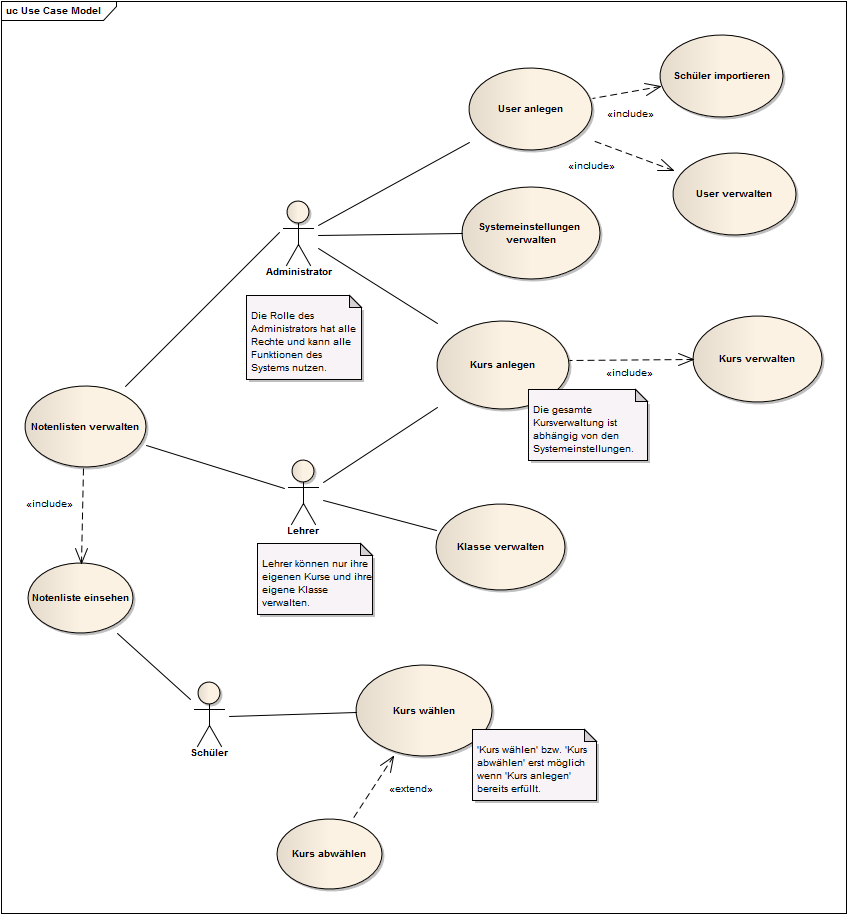
\includegraphics[scale=0.5]{img/UseCaseModel_kuwasys20.png}
 \end{center}
 \caption[\textbf{Use Case Diagram: Rollensystem}]{Use Case Diagramm: Rollensystem}
 \label{fig:UML_UC_kuwasys20}
\end{figure}

'Ein \ac{UC} beschreibt die Funktionalität des Softwaresystems, die ein Akteur ausführen muss, um ein gewünschtes Ergebnis zu erhalten oder um ein Ziel zu erreichen. \ac{UC}s sollen es ermöglichen, mit dem zukünftigen Benutzer über die Funktionalität des Softwaresystems zu sprechen, ohne sich gleich in Details zu verlieren.' Ein Zitat von \iz{Heide Balzert}{Informatikerin, die sich vor allem mit Fragen zum Thema Softwareengineering und -design beschäftigt. Derzeit ist sie Dozentin an der Fachhochschule Dortmund.}, entnommen aus \cite{BalzertH-UML2} auf Seite 28, welches den Sinn und Zweck eines \ac{UC-Diagramm}s präzise auf den Punkt bringt.

Zusammenfassend bedeutet dies, dass ein \ac{UC-Diagramm} immer dann sinnvoll ist wenn die Interaktionsmöglichkeit eines Systems, basierend auf verschiedene Aktueren, aufgezeigt werden soll. Die Akteure (dargestellt als 'Strichmännchen') im Diagramm, entsprechen genau denen, die später vom Rollensystem unterstützt werden sollen. Die Ellipsen zeigen die verschiedenen Anwendungsfälle die im System existieren. In einem so allgemeinen \ac{UC-Diagramm} wird absichtlich auf kleinste Details verzichtet. So bedeutet zum Beispiel der \ac{UC} 'Klasse verwalten' sowohl das Bearbeiten einer Klasse als auch das Vergeben von Noten oder andere klassenadministrative Aufwendungen.

Die gestrichelten Pfeile mit der Beschriftung '\texttt{$<<$include$>>$}' bezeichnen Anwendungsfälle in denen der \ac{UC}, auf welchen der Pfeil zeigt, implizit vorhanden ist wenn der \ac{UC}, von dem der Pfeil ausgeht, im System vorhanden ist. Das bedeutet wenn der \ac{UC} 'User anlegen' also vorhanden ist, auch die \ac{UC}s 'Schüler importieren' oder 'User verwalten' verwendet werden können. Ein erster \ac{UC} muss also immer erfolgen während ein zweiter (oder noch mehr) optional ausgeführt werden können.

Im Gegensatz hierzu bedeutet der gestrichelte Pfeil mit der Beschriftung '\texttt{$<<$extend$>>$}' von dem der Pfeil ausgeht, dass dieser \ac{UC} nur dann im System überhaupt vorhanden ist, wenn der \ac{UC} auf welchen der Pfeil zeigt im System vorhanden ist. Der \ac{UC} 'Kurs abwählen' ist also nur dann vorhanden wenn der \ac{UC} 'Kurs wählen' im System ausgeführt wurde. Der erste \ac{UC} wird durch den zweiten also erweitert.

\subsubsection{Statisches Analysemodell}

Im nächsten Schritt unserer Modellierung ist das statische Analysemodell, unter \prettyref{fig:UML_SA_kuwasys20} zu sehen, entworfen worden. Es stellt erste Überlegungen der Softwarearchitektur, mit konkreten Objekten inklusiver ihrer Attribute, dar und bildet ebenfalls die Beziehungen von Objekten zueinander ab. Genau genommen handelt es sich hierbei um ein 'abgespecktes' Klassendiagramm, in welchem die grobe Softwarestruktur erkennbar sein soll.

Die rechteckigen Formen stellen Klassen dar, die oben als Beschriftung ihren Namen tragen, unten die Attribute die zu ihr gehören. Die einfachen Linien sind Assoziationen zwischen den Klassen und können als Beziehungen interpretiert werden. Sie tragen einen Rollennamen und eine Multiplizität, um nachvollziehen zu können um wieviele Objekte einer Klasse es sich später mindestens und maximal handelt.
Die Rechtecke mit der Beschriftung \texttt{$<<$dataType$>>$ + String} stellen selbstdefinierte Datentypen dar.
Die Besonderheit in diesem Diagramm ist die Komposition (Assoziation mit einseitg schwarzer Raute). Sie sagt aus dass die Beziehung zwischen zwei Klassen einer starke Form der Aggregation entspricht. Die Teilklasse (Notenliste) kann also nur bestehen, solange die Aggregatklasse (Kurs) auch besteht. Würde, angewendet auf dieses Beispiel, ein Kurs gelöscht werden, würde auch der dazugehörige Notenlisteneintrag gelöscht werden. (Zur Vertiefung empfiehlt sich \cite{BalzertH_UML2} Seite 18)

In unserem Projekt entstanden zum Zeitpunkt des Softwareentwurfs 3 Klassen, die später für eine Interaktion mit dem System benötigt werden. Die Klasse für die Notenübersicht und für Kurse. Die verschiedenen Rollen wurden als Unterklassen der Klasse 'User' modelliert. Einzelne Datentypen, so bspw. für Daten zur Zeiterfassung (Datum) und zur Definition einzelner konstanter Strings (Name), wie die Rollen, wurden zur Vereinfachung vorgesehen.
Die Rollennamen sowie die Multiplizitäten der Assoziationen dürften selbsterklärend sein.

% Statisches Analyse Diagramm
\begin{figure}[H]
 \begin{center}
   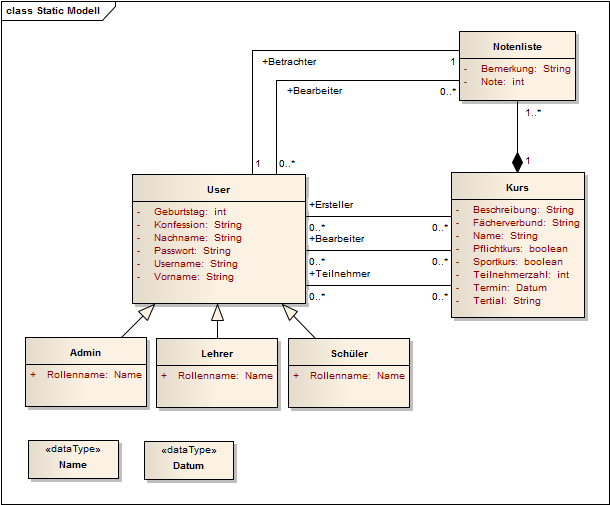
\includegraphics[scale=0.7]{img/StaticClassModel_kuwasys20.png}
 \end{center}
 \caption[\textbf{Statisches Analysemodell}]{Statisches Analysemodell}
 \label{fig:UML_SA_kuwasys20}
\end{figure}

\subsection{Benutzerschnittstellen und Rollensystem}\label{subsec:Benutzerschnittstellen und Rollensystem}

Das Kurswahlsystem der Schillerschule soll, laut Anforderungen, webbasiert mit Hilfe von verschiedenen Rollen konfiguriert und benutzt werden können.
Das System muss hierzu simultane Interaktionen, eines jeden Rollentyps, mit dem System zulassen. 

Per Aufgabendefinition liegen die vier Rollen, wie in \prettyref{subsec:Anforderungen an das System} bereits behandelt, zugrunde:

\begin{itemize}
  \item Schüler
  \item Kurslehrer
  \item Klassenlehrer
  \item Admin
\end{itemize}

Anhand der bereits vorgestellten \ac{OOM} sind, vor der Implementierung des Systems, die Rollenrechte und -richtlinien welche in den folgenden drei Unterabschnitten genaue beschrieben werden, modelliert worden.

\subsubsection{Die Rolle der Schüler}

Bei der Rolle der Schüler handelt es sich um die einfachste des Systems. 
Sie hat die wenigsten Rechte und kann hauptsächlich nur passiv, Ausnahme bildet hier die Kurswahl selbst, mit dem System interagieren.
Die Schüler welche das Kurswahlsystem erstmalig benutzen, befinden sich in der 7. Klasse. Jeder Schüler wird bis zum Abschluss der 9. Klasse das System benutzen.
Ein Schüler soll selbstständig seine Kurswahl für das jeweilige bevorstehende Tertial eines Schuljahres treffen können, dabei müssen bestimmte Abhängigkeiten eingehalten werden:

\begin{enumerate}
  \item 6 unterschiedliche Kurse pro Tertial
  \item 18 Kurse im Schuljahr
  \item 54 Kurse bis zur Vollendung des 9. Schuljahres
\end{enumerate}

\subsubsection{Die Rolle der Lehrer}

Der Rolle des Lehrers ist hingegen schon weitaus mehr Verantwortung auferlegt.
Das System unserer Webandwendung unterscheidet allerdings zwischen zwei verschiedenen Arten von Lehrern grundsätzlich nicht aufgrund einer Rollendefinition. 
Die Befugnis eines Lehrers sind lediglich abhängig von Werten die in der \ac{DB} gespeichert werden. 
Ein Klassenlehrer wird nur dann ein Klassenlehrer wenn für ihn eine Abhängigkeit zu einer Klasse besteht. 
Erst dann kann er die Funktionen, die einenm Klassenlehrer zu Verfügung stehen, nutzen.
Ein Klassenlehrer muss auf die ihm zugerordnete Klasse zugreifen und alle Kurse eines jeden Schülers einsehen können.

Das gleiche Prinzip gilt für Kurslehrer. 
Beim anlegen eines Kurses (eine Funktion die jedem Lehrer generell zur Verfügung steht) wird dieser Kurs dem Lehrer fest zugeordnet und wird somit zum Mitverantwortlichen der Kursverwaltung. 
Der Kurslehrer muss ebenfalls die Schüller einsehen können die sich in seinem Kurs befinden. Allerdings kann er nur ein Protokoll und eine Notenliste für Schüler in seinem Kurs führen.

In Abhängigkeit zur administrativen Systemverwaltung, auf die im nächsten Teil-Block eingegangen wird, hat der Lehrer nun die Rechte seine Kurse zu verwalten.

Zur Vereinfachung der Handhabung des Systems ist bereits an diesem Punkt der Modellierung an ein internes Protokollierungssystem gedacht worden. 
Es soll später die Kommunikation von Kurslehrern mit Klassenlehrern sowie die Kommunikation von Lehrern mit Schülern vereinfachen.
Im Rahmen unserer Projektarbeit wurde allerdings eine solche Funktionalität im System nicht implementiert.

\subsubsection{Die administrative Rolle des Systems}

Die administrativen Rechte des kompletten Systems stehen selbstverständlich nur dem Administrator zur Verfügung. Die Hauptaufgabe dieser Rolle im System ist es neue User ins System aufzunhemen und diese gegebenfalls zu Bearbeiten.
Das gilt für das Hinzufügen und Bearbeiten von Schülern und Lehrern gleichermaßen, beide Rollen haben also nicht die Möglichkeit sich selbst zu Verwalten.

Darüber hinaus verwaltet der Admin den Status des Systems, das aktuelle Schuljar und die dazughörigen Tertiale. Außerdem ist er der Hauptverantwortliche der Kursverwaltung.
Bevor ein Kurs stattfinden kann muss der Admin den Kurs aktivieren und für die Kurswahl zulassen. Eventuell müssen von ihm bestimmte Attribute eines Kurs noch angepasst werden können.
Ein Admin kann außerdem Fächerverbünde erstellen, bearbeiten und erstellte Kurse einem Fächerverbund zuordnen.

\subsubsection{Funktionalität des Systems}

Die Einteilung eines kompletten Schuljahrs geschieht jeweils in Tertiale. Dies kann grafisch in \prettyref{fig:Schuljahreinteilung} nachvollzogen werden. 

%%
% Schuljahreinteilung
\begin{figure}[h]
\begin{center}

\begin{tikzpicture}
    \node[draw=black, fill=yellow!20!] at (-2.5,5) {Unterteilung des Schuljahrs};
    \pie{33.3/Tertial 1, 33.3/Tertial 2, 33.3/Tertial 3}
\end{tikzpicture}

\end{center}
\caption[\textbf{Einteilung des Schuljahrs}]{Einteilung des Schuljahrs}
\label{fig:Schuljahreinteilung}
\end{figure}

Es war also nötig im administrativen Bereich des Systems eine Funktionalität vorzusehen, die es dem Admin ermöglicht das Schuljahr 'weiterzuschieben' und das entsprechende Tertial zu zu aktivieren.
Diese Verwaltungstätigkeit ist unumgänglich mit der Kurswahl verknüpft und muss für jede neu angepasst werden. 
Entscheidungen die hier während der Modellierung getroffen wurden, wurden im Hinblick auf eine möglichst einfaches \ac{UI} getroffen.

Jeder Kurs, der gewählt werden kann, gehört einem übergeordnetem Fächerverbund an, wie in \prettyref{fig:KursFaecherverbund} zu sehen ist.
Allerdings gibt es noch weitere Eigenschaften die Kurse erfüllen können. Ein Kurs kann ein Religionskurs sein, welcher für eine bestimmte Konfession ausgerichtet ist oder ein Sportkurs.
Ferner müssen Kurse als Pflichtkurse signifiziert werden können.
Aufgrund der Fülle an Informationen die verarbeitet werden müssen, war es in der Phase der Modellierung ebenfalls sehr wichtig die Datenstrukturen und deren Abhängigkeiten möglichst einfach zu halten, um in der späteren Implementierungsphase eine unkomplizierte Benutzerschnittstelle entwicklen zu können. 

%%
% Kurs - Fächerverbund
\begin{figure}[h]
\begin{center}

\begin{tikzpicture}
    \node[draw=black, fill=yellow!20!] at (-2.5,5) {Unterteilung des Schuljahrs};
    \pie{33.3/Tertial 1, 33.3/Tertial 2, 33.3/Tertial 3}
\end{tikzpicture}

\end{center}
\caption[\textbf{Einteilung des Schuljahrs}]{Einteilung des Schuljahrs}
\label{fig:KursFaecherverbund}
\end{figure}

%%
\todo[size=\small, color=green!40]{Grafik zur Abhängigkeit von Fächerverbünden bzw. Pflicht-/Sportkurse}
%%

Außer den beiden vorgestellten Datenverarbeitungen existieren selbstverständlich noch weitere, die vor allem im Sinne der Übersichtlichkeit des System  zum Tragen kommen. 
Dabei handelt es sich allerdings um Daten, die dynamisch während der Laufzeit erzeugt werden und deshalb ebenfalls in \prettyref{subsec:Systemrelevante Daten} genauer besprochen werden.
Im Gegensatz zu den dynamisch generierten Daten während der Laufzeit des Systems ist für alle anderen Daten zur Informationsverarbeitung eine Speicherung in einer Datenbank unabdingbar.
Im folgenden Unterabschnitt soll deshalb näher auf die Modellierung und Umsetzung des verwendeten Informationssystems eingegangen werden.

\subsection{Datenbankmodellierung}\label{subsec:Datenbankmodellierung}

Für die \ac{DB}-Modellierung wurde als erstes ein \ac{ER-Modell} skizziert, welches die Abhängigkeiten und Beziehungen zueinander verdeutlichen soll. Dieses ist in \prettyref{subsec:ERModell} abgebildet. Anschließend wurde das gesamte \ac{ER-Modell} in ein relationales Modell transformiert.
Mit dem entstandenen Relationalen Modell, welche in \prettyref{subsec:RelModell} dokumentiert ist, konnte anschließend auf dem Server die \ac{DB} inklusive der nötigen Tabellen erstellt werden.

\subsubsection{Entity-Relationship Modell}\label{subsec:ERModell}

Die \prettyref{fig:ERModell} zeigt das oben erwähnte \ac{ER-Modell} nach \iz{Peter Pin-Shan Chen}{Informatiker, der 1976 das ER-Modell entwickelte. Er gilt heute als Pioneer der \ac{OOM}.}, nachzulesen unter \cite{ChenPe} Seite 3 ff. bzw. \cite{VossenG-DDD} ab Seite 60.

\textbf{Aufbau des \ac{ER-Modell}s:}

Bei den blauen Rechtecken handelt es sich in diesem Modell um sogenannte Entities (Entity-Typen), die sind Dinge die in der \ac{DB} als solche abgebildet werden sollen. Sie stellen eine eigene Tabelle dar. Die gelben Ellipsen die diese umgeben, sind die Attribute (Attribut-Typen) der Entities, sie veranschaulichen die Daten welche Entities enthalten (können).
Die roten Rauten bezeichnen Beziehungen (Beziehungs-Typen) die zwischen Entities herrschen.

Das grüne Rechteck ist ein Spezialfall des 'Kurs'-Entities. Es wird als eigene Tabelle in der \ac{DB} dargestellt, ist im weitesten Sinne allerdings einer Aversion des 'Konfessions'-Attribut des 'Kurs'-Entities. Denkt man in diesem Fall an die \ac{UML}, so wäre an dieser Stelle wohl eine 'Enumeration' als eigener Datentype in Frage gekommen (Vrgl. \cite{BalzertH_UML2} Seite 10 und 11).

\tikzstyle{every entity} = [top color=white, bottom color=blue!30, draw=blue!50!black!100, drop shadow]
\tikzstyle{every weak entity} = [drop shadow={shadow xshift=.7ex, shadow yshift=-.7ex}]
\tikzstyle{every attribute} = [top color=white, bottom color=yellow!20, draw=yellow, node distance=1cm, drop shadow]
\tikzstyle{every relationship} = [top color=white, bottom color=red!20, draw=red!50!black!100, drop shadow]
\tikzstyle{every isa} = [top color=white, bottom color=green!20, draw=green!50!black!100, drop shadow]
\begin{center}
\begin{figure}[H]

\scalebox{.7}{
\begin{tikzpicture}[node distance=1.5cm, every edge/.style={link}]

%% USER
\node[entity] (usr) {Users};
\node[attribute] (usrvname) [above=2.5cm of usr] {VName} edge (usr);
\node[attribute] (usrnname) [above right=3cm of usr] {NName} edge (usr);
\node[attribute] (geb) [above left=3cm of usr] {Geburtsdatum} edge (usr);
\node[attribute] (usrkonf) [above left=of usr] {Konfession} edge (usr);
\node[attribute] (usrklasse) [above=of usr] {Klasse} edge (usr);
\node[attribute] (usrusername) [above right=of usr] {\key{Username}} edge (usr);
\node[attribute] (usrpassword) [right=of usr] {Passwort} edge (usr);
\node[attribute] (usrid) [below=0.3cm of usr] {\key{UserID}} edge (usr);

%% REL "hat"
\node[relationship] (hat) [left=1.5cm of usr] {hat} edge (usr);

%% REL "eingetragen"
\node[relationship] (eingetragen) [below left =3cm of usr] {eingetragen} edge (usr);
%
%% ROLLE
\node[entity] (rolle) [left=1cm of hat] {Rolle} edge (hat);
\node[attribute] (rollename) [left=of rolle] {\key{Username}} edge (rolle);
\node[attribute] (rolleusrnname) [above left=of rolle] {Rolle} edge (rolle);

%% REL "besucht"
\node[relationship] (besucht) [below right=of usr] {besucht} edge (usr);

%% KURS
\node[entity] (kurs) [below right=1cm of besucht] {Kurs} edge (besucht);
\node[entity, top color=white, bottom color=green!30, draw=green!50!black!100, drop shadow] (kurskonf) [above=1.5cm of kurs] {Kurskonfession} edge (kurs);
\node[attribute] (termin) [above right =.2cm of kurskonf] {Termin} edge (kurs);
\node[attribute] (kursl) [right =.2cm of kurskonf] {Kurslehrer} edge (kurs);
\node[attribute] (teilm) [above right=0.2cm of kurs] {Teilnehmerzahl} edge (kurs);
\node[attribute] (kursid) [left=0.2cm of kurs] {\key{KursID}} edge (kurs);
\node[attribute] (faecher) [right=0.2cm of kurs] {Fächerverbund} edge (kurs);
\node[attribute] (flags) [below=2.5cm of kurs] {Sportkurs} edge (kurs);
\node[attribute] (flag3) [below=2.2cm of faecher] {Pflicht} edge (kurs);
\node[attribute] (tertial) [below left=.2cm of flag3] {Tertial} edge (kurs);
\node[attribute] (flag2) [below=1.2cm of faecher] {Konfession} edge (kurs);
\node[attribute] (bemerk) [below=of kurs] {Beschreibung} edge (kurs);
\node[attribute] (kursname) [below right=0.2cm of kurs] {Kursname} edge (kurs);

%% REL "enthält"
\node[relationship] (enthalten) [below left =of kurs] {enthalten} edge (kurs);

%% NOTENLISTE
\node[entity] (notenliste) [below right=2cm of eingetragen] {Notenliste} edge (enthalten) edge (eingetragen);
\node[attribute] (note) [below left=1cm of notenliste] {Note} edge (notenliste);
\node[attribute] (usrkonf) [above =of notenliste] {Bemerkung} edge (notenliste);
\node[attribute] (usrvname) [below=of notenliste] {\key{KursID}} edge (notenliste);
\node[attribute] (usrnname) [left=of notenliste] {\key{UserID}} edge (notenliste);
\node[attribute] (listid) [below right=1.2cm of notenliste] {\key{ListenID}} edge (notenliste);

%% SYSTEM
\node[entity] (system) [below=5cm of notenliste] {System};
\node[attribute] (schuljahr) [below=of system] {Schuljahr} edge (system);
\node[attribute] (tertial) [left=of system] {Tertial} edge (system);
\node[attribute] (wochd) [below left= of system] {Phase} edge (system);
\end{tikzpicture}
}
\caption[\textbf{Entity-Relationship Modell}]{Entity-Relationship Modell}
\label{fig:ERModell}
\end{figure}
\end{center}

\textbf{Interpretation des \ac{ER-Modell}s:}

Um die Interpretation, also den Gedankengang der \ac{DB}-Modellierung, zu verdeutlichen macht es Sinn, die Beziehungen genau auszuformulieren.
Dabei werden alle Beziehungen zu jedem Entity betrachtet, begonnen mit dem Entity.
Zusätzlich sollen die Multiplizitäten mit einfließen, um die Abhängigkeiten zu verdeutlichen und um die Transformation in ein Datenbankmodell zu erleichtern.

Die Schreibweise dieser Multiplizitäten ist wie folgt definiert:

Sei $E_{A}$ das erste und $E_{B}$ das zweite Entity.
Die Beziehung beider Entities ist definiert als $R_{AB}$. 
Die erste Multipliziät $(0,N)$ gibt Auskunft über die Häufigkeit von $E_{A}$ in der geltenden Beziehung zu $E_{B}$.
Die zweite $(1;M)$ über die Häufigkeit von $E_{B}$ zu $E_{A}$.

Man kann also schreiben:

\begin{center}
$E_{A}$ ist $(0;N)$ in Beziehung $R_{AB}$ zu $E_{B}$

oder

$E_{B}$ ist $(1;M)$ in Beziehung $R_{AB}$ zu $E_{A}$
\end{center}

Wobei die erste Zahl bei der Angabe der Multiplizität, also die vor dem Semikolon (';') für die minimalste, die zweite Zahl für die maximalste Gültigkeit unter der bestendenen Bedingung steht.

Begonnen werden soll die genauere Betrachtungsweise mit dem Entity 'User':

\begin{enumerate}
  \item User - Rolle (beidseitig):	
    \begin{itemize}
      \item einem User ist genau $(1;1)$ Rolle zugeteilt
      \item einer Rolle hingegen können $(0;N)$ User zugeteilt sein
    \end{itemize}

  \item User - Kurs
    \begin{itemize}
      \item ein Schüler wählt $(0;N)$ viele Kurse
      \item ein Lehrer erstellt/verwaltet $(0;M)$ viele Kurse
    \end{itemize}
  
  \item User - Notenliste:
    \begin{itemize}
      \item ein Schüler hat $(1;1)$ Eintrag in der Notenliste für jeweils einen fest zugeordneten Kurs (Vrgl. Kurs - Notenliste)
    \end{itemize}

\end{enumerate}

Konkretisieren wir nun das Entity 'Kurs':

\begin{enumerate}
  \item Kurs - Notenliste:
  \begin{itemize}
    \item ein Kurs besitzt genau $(1;1)$ Eintrag pro Kurs in der Notenliste für einen Schüler (Vrgl. User - Notenliste)
  \end{itemize}
  
  \item Kurs - Kurskonfession	
    \begin{itemize}
      \item ein Kurs hat genau $(0;1)$ Konfessionszugehörigkeit
    \end{itemize}

  \item Kurs - User	
    \begin{itemize}
      \item ein Kurs wird von $(0;N)$ vielen Schülern gewählt
      \item ein Kurs wird immer genau $(1;1)$ Lehrern zugeteilt
    \end{itemize}
\end{enumerate}

Für das letzte Entity der Dreier-Beziehung 'Notenliste' gelten lediglich die bereits beschriebenen Abhängigkeiten und Beziehungsverhältnisse. 
Zur Verdeutlichung sollen diese jedoch nochmals aufgeführt werden.

\begin{enumerate}
  \item Notenliste - User:
  \begin{itemize}
    \item eine Notenliste hat im Bezug auf genau einen Kurs $(0;N)$ Einträge für einen User
  \end{itemize}
  
  \item Notenliste - Kurs:
  \begin{itemize}
    \item Ein Schüler wählt $(1;N)$ viele Kurse, ein Kurs wird von $(1;N)$ vielen Schülern besucht/gewählt.
  \end{itemize}
  
\end{enumerate}

Das Entity 'System' besitzt keine Beziehungen innerhalb der Datenbank, weshalb auf eine ausführliche Interpretation verzichtet werden kann.
Die Darstellung dieses Entities wird innerhalb der \ac{DB} sowieso über eine eigene Tabelle umgesetzt.

Der nächste Schritt ist nun die Transformation von \ac{ER-Modell} in das Relationale \ac{DB}-Modell.

\subsubsection{Relationales Modell}\label{subsec:RelModell}

Bei der Beschreibung des Relationalen Modells der KuWaSys-\ac{DB} ist das Hauptaugenmerk auf die komplette Datenverarbeitung gelegt, also vor allem auch Implementierungen für Vorgänge die für den Benutzer des Systems nicht unmittelbar zu sehen sind.
Daten die für die Oberfläche und die einzelnen Benutzerschnittstellen eine tragende Rolle spielen sollen unter (Abschnitt Benutzerschnittstellen) gesondert behandelt werden und werden im Laufe dieses Kapitels nur kurz angesprochen.

Die Vorüberlegungen zur Transformation von mehrwertigen Attributen von Entities sind bereits abgeschlossen.
Prinzipiell kann man mit der Transformation, wie in \cite{VossenG-DDD} beschrieben ist wie folgt vorgehen:

\begin{enumerate}
 \item Jedes Entity wird in eine relationale Form gebracht
 \item Jeder Beziehungs-Typ ebenfalls, es sei denn:
 \begin{itemize}
  \item es handelt sich um eine zweistellige $1:1$-Beziehung
  \item es handelt sich hierbei um eine $1:N$-Beziehung
 \end{itemize}
\end{enumerate}

Die Beschreibung $1:1$- bzw $1:N$-Beziehung bedeutet in diesem Fall allerdings nicht wie zuvor, ein Minimum auf der linken und das Maximum auf der rechten Seite. 
Hierbei werden nur noch die maximalen Werte der beiden Multiplizitätsangaben berücksichtigt. Dies gilt analog für alle Angaben der Multiplizitäten.

Sollte bei der Transformation $Punkt$ $2)$ eine Rolle spielen, müssen Attribute in bereits bestehende Relationsschemata aufgenommen werden. Folgende Regeln treten dann in Kraft:
\begin{enumerate}
 \item Zweistellige $1:1$-Beziehung
 \begin{itemize}
  \item ein Entity stellt selbst ein Relationsschema dar
  \item Attribute des zweiten Entities werden ebenfalls in dieselbe Tabelle gespeichert
 \end{itemize}
 \item Zweistellige $1:N$-Beziehung
 \begin{itemize}
  \item ein Entity stellt ein eigenes Relationsschema dar
  \item erste Möglichkeit: die Attribute des Entities welches die maximale Multiplizität von $1$ aufweist wird hingegen dem Realtionsschema mit der maximalen Multiplizität von $N$ in Form von Fremdschlüsseln zugeschrieben
  \item zweite Möglichkeit: es wird ein eigenes Relationsschema für die Beziehung der beiden Entities angelegt. Dieses neu entstande Schema erhält dann Attribute, welche widerum Fremdschlüssel der beiden anderen Entities sind
 \end{itemize}
\end{enumerate}

Die Transformation vom \ac{ER-Modell} ins Relationale Modell (zur bildhaften Darstellung ist die Kopfzeile der dazugehörigen Tabelle auch gezeigt) sieht im Falle des Kurswahlsystems folgendermaßen aus:

\textbf{Users} = \{( \underline{id:serial}, nachname:character, vorname:character, geburtstag:character, konfession:character, klasse:character, \underline{username:character}, passwort:character )\}

% User-Tabelle
\begin{table}[H]
\begin{center}
	\begin{tabular}{|c|c|c|c|c|c|c|c|}\hline
		\textbf{\underline{ID}} & \textbf{NName} & \textbf{VName} & \textbf{Geb} & \textbf{Konf} & \textbf{Klasse} & \textbf{\underline{Username}} & \textbf{Passwort} \\ \hline
		\vdots & \vdots & \vdots & \vdots & \vdots & \vdots & \vdots & \vdots \\
	\end{tabular}
	\caption{Kopfzeile der User-Tabelle}
\end{center}
\end{table}

\textbf{Kurs} = \{( \underline{id:serial}, name:character, kurslehrer:integer, faecherverbund:character, termin:integer, beschreibung:character, schuljahr:integer, tertial:integer, 
teilnehmerzahl:integer, pflichtkurs:boolean, sport:boolean )\}

% Kurs-Tabelle
\begin{table}[H]
\begin{center}
	\begin{tabular}{|c|c|c|c|c|c}\hline
		\textbf{\underline{ID}} & \textbf{Name} & \textbf{Kurslehrer} & \textbf{Faecherverbund} & \textbf{Termin} & \dots \\ \hline
		\vdots & \vdots & \vdots & \vdots & \vdots & \dots \\
	\end{tabular}
	\caption{Kopfzeile der Kurs-Tabelle  (unvollständig)}
\end{center}
\end{table}

\textbf{Kurs-Konfessionen} = \{( \underline{religionid:integer}, konfession:character )\} 
 
% Kurs-Konfession-Tabelle
\begin{table}[H]
\begin{center}
	\begin{tabular}{|c|c|}\hline
		\textbf{\underline{ReligionID}} & \textbf{Konfession} \\ \hline
		\vdots & \vdots \\
	\end{tabular}
	\caption{Kopfzeile der Kurs-Konfessions-Tabelle}
\end{center}
\end{table}

\textbf{Notenliste} = \{( \underline{id:serial}, note:integer, bemerkung:character, userid:integer, kursid:integer, jahr:integer, tertial:integer )\}

% Notenliste-Tabelle
\begin{table}[H]
\begin{center}
	\begin{tabular}{|c|c|c|c|c|c|c|}\hline
		\textbf{\underline{ID}} & \textbf{Note} & \textbf{Bemerkung} & \textbf{UserID} & \textbf{KursID} & \textbf{Jahr} & \textbf{Tertial}\\ \hline
		\vdots & \vdots & \vdots & \vdots & \vdots & \vdots & \vdots  \\
	\end{tabular}
	\caption{Kopfzeile der Notenlisten-Tabelle}
\end{center}
\end{table}

\textbf{Rolle} = \{( \underline{username:character}, rolle:character )\}

% Rollen-Tabelle
\begin{table}[H]
\begin{center}
	\begin{tabular}{|c|c|}\hline
		\textbf{\underline{Username}} & \textbf{Rolle} \\ \hline
		\vdots & \vdots \\
	\end{tabular}
	\caption{Kopfzeile der Rollen-Tabelle}
\end{center}
\end{table}

\textbf{System} = \{( \underline{phase:integer}, jahr:integer, tertial:integer )\}

% System-Tabelle
\begin{table}[H]
\begin{center}
	\begin{tabular}{|c|c|c|}\hline
		\textbf{\underline{Phase}} & \textbf{Jahr} & \textbf{Tertial} \\ \hline
		\vdots & \vdots & \vdots \\
	\end{tabular}
	\caption{Kopfzeile der System-Tabelle}
\end{center}
\end{table}

\subsection{Konfiguration der Laufzeitumgebung und des Servers}\label{subsec:Konfiguration der Laufzeitumgebung und des Server}

Dieses Kapitel ist als Zwischenschritt, von der Modellierung zur Implementierung, unseres Softwareprojekts zu verstehen.
Zum Einen galt es eine komplette bestehende Infrastruktur zu überblicken und zu verstehen (dieser Schritt kann als eine Art der Modellierung verstanden werden)
zum Anderen musste ein komplettes neues System einwandfrei funktionsfähig eingebettet werden (zu vergleichen mit dem Schritt der Implementierung).

\textbf{Sichtung der bestehenden Infrastruktur:}

Die Schillerschule teilt sich mit der benachbarten Realschule am Galgenberg eine Serverinfrastruktur nach der Novell Musterlösung paedML 3.33, weitere Informationen sind unter \cite{paedML} zu finden. % VMWare ASG 220 Astaro.
Diese beinhaltet eine virtuelle Infrastruktur \gls{VMWare} ESXi auf der ein \ac{SLES} Novell Server gehostet ist.

\begin{figure}[H]
\begin{center}
\begin{tikzpicture}[
  scale=0.1,
  font=\sffamily,
  every matrix/.style={ampersand replacement=\&,column sep=2cm,row sep=2cm},
  source/.style={draw,thick,rounded corners,fill=yellow!20,inner sep=.3cm},
  process/.style={draw,thick,circle,fill=blue!20},
  sink/.style={source,fill=green!20},
  datastore/.style={draw,very thick,shape=datastore,inner sep=.3cm},
  dots/.style={gray,scale=2},
  to/.style={->,>=stealth',shorten >=1pt,semithick,font=\sffamily\footnotesize},
  every node/.style={align=center}]

  % Positionierung über Matrix-Layout
  \matrix{

    \node[source] (Ubuntu) {Ubuntu 12.04 VM\\ ($141.10.50.250$)};
      \& \node[process] (Suse) {Server}; \& \\
      \& \node[sink] (firewall) {ASG 220 Astaro\\ ($Firewall$)}; \& \\

    \node[source] (SLES) {SuSE Linux\\ Enterprise Server\\ ($SLES$)}; \& \\

    \node[datastore, color=black!50!white] (infrastructure) {Einstellungen\\($Novell$ $paedML$ $3.3$)}; \& \\


      \& \node[process] (router) {Router};
      \& \node[sink] (www) {WWW}; \\
  };

  % VM - Host
  \draw[to, very thick] (Ubuntu) -- node[midway,above] {VM Host}
      node[midway,below] {} (Suse);

  % FW - Host
  \draw[to, dashed, very  thick] (Suse) -- node[midway,above] {}
       node[midway,below] {} (firewall);itemize
  \draw[to, dashed, very  thick] (firewall) -- node[midway,above] {}
       node[midway,below] {} (Suse);

  % FW - Router
  \draw[to, very thick] (router) -- node[midway,above] {}
       node[midway,below] {} (firewall);
  \draw[to, very  thick] (firewall) -- node[midway,above] {}
       node[midway,below] {} (router);

  % Einstellungen Infrastruktur
  \draw[color=black!50!white] (infrastructure) -- node[midway,above] {}
       node[midway,below] {} (SLES);

  % SLES - Netz
  \draw[to, very thick] (SLES) -- node[midway,above=1cm] {VM Host}
       node[midway,below] {} (Suse);
  \draw[to, dashed, color=black!50!white] (SLES) -- node[midway,right=0.2cm] {Konfiguration}
       node[midway,below] {} (router);
  \draw[to, dashed, color=black!50!white] (SLES) -- node[midway,right=0.2cm] {Konfiguation}
       node[midway,below] {} (Ubuntu);

  % Router - WWW
  \draw[to, very thick] (router) -- node[midway,above] {}
       node[midway,below] {} (www);
  \draw[to, very thick] (www) -- node[midway,above] {}
       node[midway,below] {} (router);
\end{tikzpicture}
\end{center}
\caption[\textbf{Netzwerkstruktur der Schillerschule Aalen}]{Netzwerkstruktur der Schillerschule Aalen mit DMZ}
\label{fig:Netzwerkstruktur}
\end{figure}

Prinzipiell wäre eine Verwendung dieser virtuellen \gls{Appliance} zum Hosting der \ac{Webapp} möglich. Um jedoch die Systemsicherheit zu erhöhen ist eine weitere virtuelle Appliance, die nur das Kurswahlsystem bereitstellt die bessere Wahl.
\iz{Ubuntu Server 12.04 LTS}{http://www.ubuntu.com/} läuft auf diesem virtuellen Rechner, der sich wie der oben genannte SLES in der \gls{DMZ} der virtuellen Netzwerkinfrastruktur befindet.

\textbf{Integration in die Infrastruktur:}

Ein PostreSQL-Server dient zur Datenhaltung und ein Apache Tomcat 7 zur Auslieferung der \ac{Webapp}. Nach Konfiguation (und überfälligem reboot) der Astaro Firewall im Keller der Schule ist die Webapp jetzt über das Intranet an allen Rechnern im Schulnetz erreichbar (\url{http://192.168.1.222:8080/kuwasys20}). Die Erreichbarkeit über das Internet ist seit der Freischaltung der entsprechenden Ports auf den BelWü-Server und umgekehrt gegeben (\url{http://141.10.50.250:8080/kuwasys20}).
Diese Adressen werden auf der Homepage der Schillerschule und im Intranet verlinkt, sodass keine weitere Maskierung wie Subdomains oder lokale DNS-Einträge notwendig ist.
Die Admnistration des Ubuntu Servers kann im Intranet von einer VMWare Management Console aus erfolgen, für schnelles Eingreifen wurde ein \gls{Secure Shell} (SSH) Zugang eingerichtet, der im Internet erreichbar ist.

In \prettyref{fig:Netzwerkstruktur} ist die neue Struktur des Netzwerks dargestellt.

Die Einrichtung eines Backups war für unser Projekt nicht notwendig, da die Schillerschule selbst schon über ein funktionsfähiges Backupsystem verfügt. Hierbei wird in bestimmten Intervallen die komplette Festplatte des Servers gespiegelt, und somit auch die virtuellen Maschinen.
Somit ist die Garantie gegeben, dass auch das Kurswahlsystem einem ständigen Sicherungsvorgang unterliegt und im Notfall wiederhergestellt werden kann.
\newpage

\section{Implementierung}	\label{sec:Implementierung}
							\label{secmin:Implementierung}

In einem System, in welchem ein \gls{Multi-User Betrieb} möglich sein soll, ist das Design der Oberfläche und das der einzelnen Benutzerschnittstellen unweigerlich eng miteinander verknüpft. 
Es müssen in der Phase der Implementierung bereits exakte Schnittstellen definiert und strukturierte Oberflächen skizziert worden sein um spätere Korrekturen gering zu halten oder um sie zu vermeiden.

In den folgenden zwei Abschnitten sollen grundlegende Implementierungsgedanken besprochen werden, die mit den Anforderungen an das System in erster Linie nichts zu tun haben. 
Zuerst soll die Art und Weise der Umsetzung der Benutzerschnittstellen und des Designs näher erklärt werden. Danach sollen elementare Datenstrukturen die zum Einsatz kamen und in JSF implementiert wurde näher erläutert werden.

Nach den beiden einführenden Abschnitten wird dem Leser detailiert dargestellt wie die zu bewältigenden Systemanforderungen in JSF umgesetzt wurden. 
Dabei werden Quellcodeausschnitte sowie Diagramme zum Einsatz kommen die dem Leser das Verstehen erleichtern sollen.
Da während allen Phasen der Umsetzung des Projekts auch immer die Modularität des gesamten Systems im Vordergrund stand soll hier nicht kleinlichst genau erklärt werden was im Quellcode steht, sondern darauf eingegangen werden, wie das zu lösende Problem angegangen wurde und schlussendlich welche wichtigen Bausteine zu tragen kamen. 
An dieser Stelle soll außerdem nochmals die Wichtigkeit der oben besprochenen Datenbankmodellierung erwähnt werden. Gründe für die verschiedenen Umsetzungen der Modellierung sollen im Abschnitt der Implementierung dieser Ausarbeitung nicht mehr näher besprochen werden. 
Es wurde jedoch viel Wert darauf gelegt die Schritte der Implementierung gut und verständlich zu formulieren und darzustellen.

\subsection{Benutzerschnittstellen und Oberflächendesign}

Wir haben uns für ein simples und einfach zu verstehendes Oberflächendesign entschieden, welches allerdings den Design Aspekten der \gls{Corporate Identity} (CI) erfüllen sollte. 
%%
\todo[size=\small, color=green!40]{HMI Buch Zitate etc...}
%%
Im allgemeinen wird beim Screendesign bestimmten Regeln gefolgt, welche durch das gewählte Gestaltungsraster festgelegt werden.

Hierzu wurden von uns folgende Bereiche festgelegt:
\begin{itemize}
  \item Kopf- oder Bannerbereich mit Logo
  \item Navigationsbereich bzw. Unternavigation
  \item Arbeitsbereich
  \item Impressum/Hinweise
\end{itemize}

Der Hauptaufbau dieser Seiten, auf welche im folgenden näher eingegangen wird, wurden mit Templates, wie es bereits in \prettyref{subsec:Darstellung von Seiteninhalten} angesprochen wurde, umgesetzt.
Der allgemeine Aufbau soll im folgenden besprochen werden, der nachstehende Quellcodeausschnitt zeigt einen Teil des Templates das von uns zur Gestaltung der Seiten verwendet wurde:

% LISTING
% template.xhtml 
%%
\todo[size=\small, color=red!40]{Listing}
%%
Auffallend ist vor allem der Kopf der Seite, welcher den Wiedererkennungswert (Vrgl. hierzu die \iz{Webiste der Schillerschule}{\url{http://www.schillerschule-aalen.de}}) ganu im Sinne des \ac{CI}s steigern soll.
Hierzu wurde die Grafik lediglich transparenter gehalten als ihr Original und hat ganz im Stil der Schule die Überschrift erhalten wie in \prettyref{fig:header_KuWaSys} zu sehen ist.

% Header
\begin{figure}[H]
 \begin{center}
   
\includegraphics[scale=0.4]{img/header_KuWaSys.png}
 \end{center}
 \caption[\textbf{KuWaSys: Banner des Systems (Header)}]{KuWaSys: Banner des Systems (Header)}
 \label{fig:header_KuWaSys}
\end{figure}

Die Navigation und deren Unternavigationspunkte sind im linken Bereich der Webiste angeordnet und unterstützen den User visuell mit Hervorhebungen, wie in \prettyref{fig:navihervorhebung_KuWaSys} dargestellt ist, bei der Arbeit mit dem System.
Nötige Unternavigationspunkte, falls diese vorhanden sind, öffnen sich automatisch beim Klick auf ein übergeordnetes Menüelement, sodass die komplette Menüstruktur handlich und kompakt dargestellt erscheint und mit einem Blick erfasst werden kann.

Der Arbeitsbereich wird in der Mitte der Seite dargestellt, unterhalb des Kopfbereichs und rechts der Navigation. 
Dieser wird abgetrennt durch blaue Balken (links zur Navigation sowie oben zum Kopfbereich) um die Einteilung der Seite für die Benutzer des Systems eindeutig und übersichtlich zu halten.
Jede Interaktion mit dem System wird in diesem Bereich der Website dargestellt. 
%%
\todo[size=\small, color=green!40]{Grafik zu Bildschirmenteilung}
%%

% Infobar
\begin{figure}[h]
 \begin{center}
   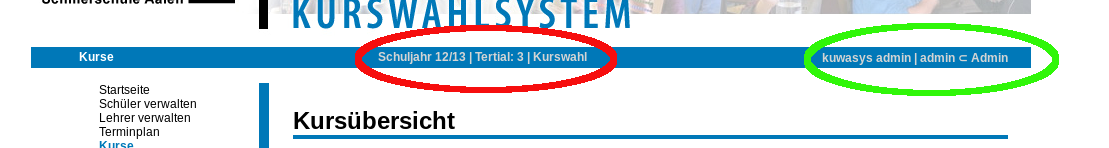
\includegraphics[scale=0.4]{img/informationbar_KuWaSys.png}
 \end{center}
 \caption[\textbf{KuWaSys: Informationsbalken (oberer Bereich)}]{KuWaSys: Informationsbalken (oberer Bereich)}
 \label{fig:infobar_KuWaSys}
\end{figure}

Zur erwähnen ist zudem noch der Trennbalken nach oben welcher zusätzlich als Informationsanzeige für den User verwendet wird und der Fußbereich welcher Informationen zur Website enthält. 
Die obere Anzeige, hier werden Informationen zum User selbst (Voller Name, Username und Rolle im System) und Informationen zum aktuellen Status des Systems (aktuelles Schuljahr und aktuelles Tertial) angezeigt.
Die \prettyref{fig:infobar_KuWaSys} zeigt die genaue Einteilung des Infobalkens oben, rot die Informationen des Systems, grün die Informationen des Users.
Der Fußbereich dient ausschließlich zur weiteren Information beim Besuch der Webiste welcher in \prettyref{fig:footer_KuWaSys} zu sehen ist.  

Die Hauptfarben des Systems wurden absichtlich blau gewählt um eine gewisse Professionalität sowie Seriösität gegenüber den Benutzern auszustrahlen. Diese ziehen sich kontinuierlich durch das gesamte System

%%
\todo[size=\small, color=green!40]{HMI Buch Dahm...}
%%

% Navibar
\begin{wrapfigure}[18]{r}{12cm}
 \begin{center}
   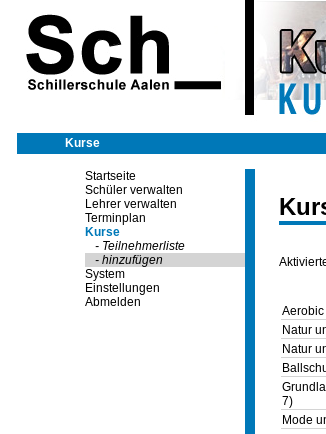
\includegraphics[scale=0.65]{img/navigation_KuWaSys.png}
 \end{center}
 \caption[\textbf{KuWaSys: Navigations und Menüelemente (linker Bereich)}]{KuWaSys: Navigations und Menüelemente (linker Bereich)}
 \label{fig:navihervorhebung_KuWaSys}
\end{wrapfigure}

Auf ein Impressum oder auf rechtliche Hinweise konnte bei dieser Art von Webiste verzichtet werden. 
Erstens handelt es sich hierbei um keine kommerzielle Website, laut \textit{§5} \ac{TMG} wird ein Impressum von 'geschäftsmäßigen Online-Diensten' benötigt, 
%%
\todo[size=\small, color=green!40]{rechtlicher Nachweis} zweitens um keine öffentliche oder frei zugängliche Website, 
%%
wobei hier die Vorschrift des \textit{§55} \ac{RstV} besagt, dass eine Impressumspflicht nur dann besteht wenn der Inhalt der Website regelmäßig journalistisch-redaktionelle Inhalte online zur Verfügung stellt.
(Gesetzesauszüge sind im Anhang unter \prettyref{subsec:Gesetz} zu finden) 

% Footer
\begin{figure}[h]
 \begin{center}
   
\includegraphics[scale=0.7]{img/footer_KuWaSys.png}
 \end{center}
 \caption[\textbf{KuWaSys: Informationsbalken (unterer Bereich)}]{KuWaSys: Informationsbalken (unterer Bereich)}
 \label{fig:footer_KuWaSys}
\end{figure}

Zur Strukturierung von Seiteninhalten wurden herkömmliche \ac{JSF}-Standardkomponenten verwendet.
Zu den hauptsächlich verwendeten, zählen:
\begin{itemize}
  \item \texttt{<h:outputText>}\\
    Element welches HTML-Text auf der Obefläche ausgibt 
  
  \item \texttt{<h:outputLabel>}\\
    auch normaler Text, allerdings als Beschriftung von Texteingabefeldern
      
  \item \texttt{<h:inputText>}\\
    Element zur Texteingabe, Synonyme für ein HTML \texttt{<input>}-Tag mit type="text"
  
  \item \texttt{<h:inputSecret>}\\
    Element zur verschlüsselten Texteingabe, entspricht \texttt{<input>}-Tag mit type="password"
  
  \item \texttt{<h:commandButton>}\\
    Button in HTML, der Klick löst eine definierte Aktion über eine ManagedBean-Methode aus

  \item \texttt{<h:panelGrid>}\\
    Darstellung einer Tabelle, Synonym für das HTML \texttt{<table>}-Tag. Die Anzahl der Spalten wird über das \texttt{columns}-Attribut festgelegt
  
  \item \texttt{<h:panelGroup>}\\
    Container-Element (mehrere JSF-Tags werden zu einem zusammenfügt)
  
  \item \texttt{<h:message>}\\
    gibt eine Fehlermeldung für die definierte Komponenten aus (\texttt{ErrorStyle}-Attribut über \ac{CSS} steuerbar)
  
  \item \texttt{<h:form>}\\
    stellt ein Formular dar, welches einen POST-Request per HTTP absetzt
  
  \item \texttt{<f:facet>}\\
    Definiert eine Facette (bspw. die Überschrift für eine Tabelle)
\end{itemize}

Außer den eben erwähnten Komponenten gibt es eine Vielzahl anderer bis hin zu selbstdefinierten welche im entwickelten System zum Einsatz kommen. Diese werden allerdings nicht näher betrachtet, da sie für das umgesetzte System irrelevant sind. Selbstverständlich kann zur grafischen Darstellung auch normale \ac{HTML}-Syntax verwendet werden.
Um die Strukturierung des Seitenaufbaus übersichtlich zu halten wird ebenfalls das wohl bereits bekannte Grundlagenwerkezug der Webentwicklung, die \gls{Cascading Style Sheets} (CSS), für die Eigenschaften der Darstellungselemente, eingesetzt.
Vorteile dieser Vorgehensweise der Datenverarbeitung resultiert in einer einheitlichen und damit gut strukturierten Darstellung der betroffenen Websites.

%%
\todo[size=\small, color=green!40]{CSS/Komponenten Listings}
%%

\subsection{Informationsdarstellung und -verarbeitung}

Eine elementare Datenstrukturen im System sind Listen, welche dem User in Form einer Tabelle dargestellt werden.
Die Vorteile dieser Datenstruktur sind die Einfachheit der Datenhaltung sowie der Zugriff auf die Daten und Bereitstellung dieser.

Grundlegend sind zwei zu unterscheidende Listen im System implementiert:
\begin{enumerate}
  \item User-Listen (Schüler und Lehrer)
  \item Kurs-Listen
  \item Noten-Listen
\end{enumerate}

Dabei sind beide Listen lediglich nach Art des Inhalts ihrer Daten zu differenzieren. Die für die Benutzeroberfläche relevanten sollen kurz erläutert werden:

\textbf{Schüler}
\begin{itemize}
  \item ID: Integer, welcher für das Wählen von Kursen und das Vergeben von Noten wichtig ist, da diese einen Fremdschlüssel in der jeweiligen Tabelle darstellt
  \item Vorname und Nachname: String, der den realen Namen des Users wiedergibt
  \item Klasse: String, zur Identifizierung welchem Klassenlehrer ein Schüler zugeordnet ist, bzw wie weit er in seiner Schullaufbahn vorangeschritten ist
  \item Konfession: String, zur Identifizierung des Religionsunterrichts der angeboten werden kann bzw. muss während dem Erstellen eines Kurses. (Näheres in Abschnitt Kurswahl)
\end{itemize}

\textbf{Lehrer}
\begin{itemize}
  \item ID (mit der gleichen Bedeutung wie bei Schülern)
  \item Vorname und Nachname (ebenfalls gleich wie bei Schülern)
  \item Klasse: String, der festlegt, von welcher Klasse ein Lehrer Klassenlehrer ist
\end{itemize}

\textbf{Kurse}
\begin{itemize}
  \item Kursnummer
  \item Kursname
  \item Kursbeschreibung
  \item Teilnehmeranzahl
\end{itemize}

\textbf{Notenlisten}
\begin{itemize}
  \item Schülername
  \item Kursname
  \item Note
  \item Bemerkung
\end{itemize}

Die Implementierung der Listen in Java wurde über Listen vom Typ \texttt{ArrayList<List>} umgesetzt. 
%%
\todo[size=\small, color=orange!40]{technische Umsetzung von Listen, Grundlagen etc... am Beispiel von Java Listings - 1 bis 2 Getter/Setter}
%%
%%
\todo[size=\small, color=orange!40]{dazugehöriges Facelet, bpw. Schüler}
%%
%%
\todo[size=\small, color=orange!40]{Datenbankabfrage und 'Befüllen' der Listen}
%%


\subsection{Benutzerauthentifizierung}

Einer der elementarsten Vorgänge im System ist der Login-Vorgang. Es handelt sich hierbei um einen Vorgang den jeder Benutzer egal mit welcher Rolle vor der Interkation mit dem System durchlaufen muss. Zur Verifizierung eines Users am System wird sein Kürzel, welches beim Anlegen automatisch aus Vor- und Nachnamen generiert wird, sowie ein Passwort, welches ebenfalls automatisch und randomisiert generiert wird, benötigt. Die Anmeldemaske, welche zugleich auch die Startseite des Kurswahlsystems bildet, kann in \prettyref{fig:login_KuWaSys} angesehen werden. Die Registrierung eines Users am System kann ausschließlich durch den Admin erfolgen.

% Login
\begin{wrapfigure}[12]{l}{10cm}
 \begin{center}
   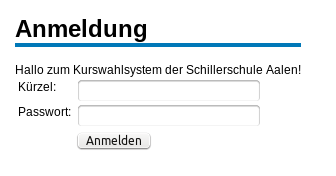
\includegraphics[scale=0.7]{img/login_KuWaSys.png}
 \end{center}
 \caption[\textbf{KuWaSys: Login Maske und Startseite}]{KuWaSys: Login Maske und Startseite}
 \label{fig:login_KuWaSys}
\end{wrapfigure}


Für den Vorgang des Logins am System besitzt der Servlet-Container Tomcat 7 eine sehr hilfreiche und gängige Funktion der Softwareentwicklung, die Konfiguation des \ac{DBCP}s des Apache Commons Projekts. Nähere Informationen sind unter \cite{ApacheDBCP} zu finden. 

Wie bereits aus dem \prettyref{subsec:Datenbankmodellierung} bekannt ist, haben wir für unser Datenbank eine zusätzliche Tabelle 'Rolle', die mit der Tabelle 'User' in Relation steht, modelliert. Diese wird nun für die Konfiguration des \ac{DBCP}s benötigt.

Der \ac{DBCP} gehört zu einer Art

Aufgrund der Tatsache, dass die Rollen-Tabelle mit der User-Tabelle in einer Beziehung zueinander steht, kann bei der Authentifizierung also genau auf den gewollten User zugegriffen werden. Diese Tatsache machen wir uns auch im weiteren Verlauf der Systemimplementierung zu Nutze, bspw. bei der Generierung von Benutzerdaten (\prettyref{subsec:Daten eines Benutzers}) oder aber um Daten zu manipulieren die mit dem User in Verbindung stehen.

%%
\todo[size=\small, color=orange!40]{Datenbankabfrage und Check Methoden Listing}
%%
 

\subsection{Benutzerverwaltung}\label{subsec:Daten eines Benutzers}
%%
\todo[size=\small, color=red!40]{Eindeutigkeit von Usernamen/Passwort bei Generierung}
%%

\subsubsection{Anlegen von Benutzerdaten}

Das Anlegen eines Benutzers erfordert immer die Informationen über:
\begin{itemize}
  \item Vor- und Nachname
  \item Geburtsdatum
  \item Klasse
  \item Konfession
\end{itemize}

Die Rolle, die ein Benutzer im System erhält, wird durch zwei unterschiedlich Eingabeaufforderungsdesigns umgesetzt. Eines für Lehrer und eines für Schüler. Benutzernamen und Passwörter werden vom System anhand der eingegebenen Informationen automatisch generiert. 

% User anlegen: Schüler
\begin{figure}[H]
 \begin{center}
   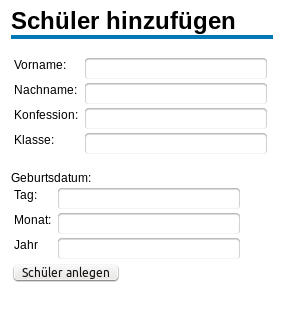
\includegraphics[scale=0.6]{img/UserAnlegen_KuWaSys.png}
 \end{center}
 \caption[\textbf{KuWaSys: User anlegen}]{KuWaSys: User anlegen}
 \label{fig:UserAnlegen_KuWaSys}
\end{figure}


% User anlegen: Lehrer
\begin{figure}[H]
 \begin{center}
   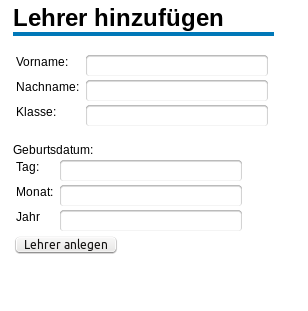
\includegraphics[scale=0.6]{img/LehrerAnlegen_KuWaSys.png}
 \end{center}
 \caption[\textbf{KuWaSys: Lehrer anlegen}]{KuWaSys: Lehrer anlegen}
 \label{fig:LehrerAnlegen_KuWaSys}
\end{figure}

textbf{Sonderfunktion: CSV-Import}

Eine Besonderheit der Benutzerverwaltung ist der Import von Userdaten über \ac{CSV}-Dateien. Diese Funktion war im Sinner der Projektarbeit nicht gefordert erleichtert aber die Arbeit mit dem System ungemein. Da jedes Jahr, zum Schuljahresbeginn, neue Schüler in das Kursplanungs- und Kurswahlsystem mit aufgenommen werden müssen wäre der Aufwand einzelne Benutzer hinzuzufügen zu groß und langwierig. Außerdem werden CSV-Dateien auch von gängigen Tabellenkalkulationsprogrammen unterstützt.

Als Vorlage für erste Importversuche diente die aktuelle Schülerliste im CSV-Format. Diese enthielt Daten in der Form:
%% Listing: CSV Schüler
	\lstinputlisting[label={lst:schiller_schueler.csv},
	caption={Beispiel einer CSV-Datei mit User Informationen},
	frame=tlbr, 
	language=java, 
	breaklines=true, 
	numbers=left, 
	numberstyle=\tiny, 
	stepnumber=1, 
	numbersep=5pt, 
	basicstyle=\small\ttfamily,
	showstringspaces=true,
	keywordstyle=\bfseries\color{lila}, 
	backgroundcolor=\color{lightgrey}]{listings/schiller_schueler.csv}

Mit Hilfe dieser Datei konnte ein Parser entworfen werden. Umgesetzt wurde der Parser mit der JAVA-Klasse \texttt{StringTokenizer}, um Tokens zu definieren und nach ihnen zu selektieren, und mit der Klasse \texttt{BufferedReader} und \texttt{InputStreamReader}, um die CSV-Datei überhaupt erst einlesen zu können. 

Der \prettyref{lst:ImportBean.java} zeigt die ManagedBean-Klasse \texttt{importBean} mit der Methode \texttt{doImport()}, die den komplettem Parse-Vorgang einer CSV-Datei steuert.
Die wichtigsten Zeilen des Quellcodeausschnitts sollen kurz erläutert werden:
\begin{itemize}
  \item[Zeile]
  \item[08:] Initialisierung der String-Variablen
  \item[23:] Beginn des Parsing-Vorgangs: Solange die CSV-Datei weitere Zeilen enthält
  \item[25:] Initialisierung des StringTokenizers (Zeilen und Angabe des Trennzeichens)
  \item[26:] Zeilenweise Tokens auswählen, solange weitere Tokens existieren
  \item[28:] Switch-Case fängt Integer-Wert der Tokens ab und weist die Werte den richtige Strings zu
  \item[47:] Aufruf der Methode \texttt{addUser} der \texttt{DatabaseHandler}-Klasse, die als Paramter die ausgelesenen Informationen der CSV-Datei enthält und einen neuen User im System anlegt
\end{itemize}

Wie unschwer zu erkennen ist, ist der Parser sehr einfach gestrickt. Es reicht anzugeben welche Trennzeichen zwischen den Daten benutzt werden (Obwohl der Namen CSV als Trennzeichen das Komma suggeriert, können als Trennzeichen zumindest auch Semikoli verwendet werden).
Weiter ist es ausreichend zu wissen wann die CSV-Datei endet und schlussendlich wie die Reihenfolge, der Werte die ausgelesen werden sollen, ist.

%% Listing: CSV Schüler - Parser
	\lstinputlisting[label={lst:ImportBean.java},
	caption={CSV-Datei Parser-Methode},
	frame=tlbr, 
	language=java, 
	breaklines=true, 
	numbers=left, 
	numberstyle=\tiny, 
	stepnumber=1, 
	numbersep=5pt, 
	basicstyle=\small\ttfamily,
	showstringspaces=true,
	keywordstyle=\bfseries\color{lila}, 
	tabsize=2,
	backgroundcolor=\color{lightgrey}]{listings/ImportBean.java}

\subsection{Kursverwaltung}

Neben dem Anlegen von neuen Benutzern, muss das System auch die Funktionalität besitzen, neue Kurse hinzuzufügen.

%%
\todo[size=\small, color=red!40]{Kurs anlegen (Lehrer)/Kurs aktivieren (Admin)/Kurs wählen (Schüler) !!!auch Diagramm!!!}
%%

Darstellung des Stundenplans:
\begin{figure}[H]
\centering
\begin{tikzpicture}[x=\daywidth, y=-1cm, node distance=0 cm,outer sep = 0pt]
% Style for Days
\tikzstyle{day}=[draw, rectangle,  minimum height=1cm, minimum width=\daywidth, fill=yellow!20,anchor=south west]
% Style for hours
\tikzstyle{hour}=[draw, rectangle, minimum height=1 cm, minimum width=1.5 cm, fill=yellow!30,anchor=north east]

% Styles for events
% Dauer Stunden
\tikzstyle{hours}=[rectangle,draw, minimum width=\daywidth, anchor=north west,text centered,text width=5 em]
\tikzstyle{1hour}=[hours,minimum height=1cm]
\tikzstyle{2hours}=[hours,minimum height=2cm]
\tikzstyle{3hours}=[hours,minimum height=3cm]

% Style der Fächer
\tikzstyle{Kern}=[2hours,fill=green!20]
\tikzstyle{Kurs1}=[2hours,fill=red!20]
\tikzstyle{Kurs2}=[2hours,fill=blue!20]
\tikzstyle{Kurs3}=[2hours,fill=blue!10]
\tikzstyle{Kurs4}=[2hours, pattern=north east lines, pattern color=magenta]
\tikzstyle{Kurs5}=[3hours, pattern=north west lines, pattern color=magenta!60!white]s
\tikzstyle{Planche}=[1hour,fill=white]

% Positioning Tag/Stunden
\node[day] (mo) at (1,8) {Montag};
\node[day] (di) [right = of mo] {Dienstag};
\node[day] (mi) [right = of di] {Mittwoch};
\node[day] (do) [right = of mi] {Donnerstag};
\node[day] (fr) [right = of do] {Freitag};

\node[hour] (8-9) at (1,8) {8-9};
\node[hour] (9-10) [below = of 8-9] {9-10};
\node[hour] (10-11) [below= of 9-10] {10-11};
\node[hour] (11-12) [below = of 10-11] {11-12};
\node[hour] (12-13) [below  = of 11-12] {12-13};
\node[hour] (13-14) [below = of 12-13] {13-14};
\node[hour] (14-15) [below = of 13-14] {14-15};
\node[hour] (15-16) [below = of 14-15] {15-16};
\node[hour] (16-17) [below = of 15-16] {16-17};
\node[hour] (17-18) [below = of 16-17] {17-18};
\node[hour] (18-19) [below = of 17-18] {18-19};

% Position Fächer
\node[Kurs1] at (1,10) {Sport};
\node[Kern] at (1,8) {D/M/E};
\node[Kern] at (2,8) {Physique};
\node[Kern] at (4,8) {Physique};
\node[Kern] at (5,10) {Physique};
\node[Kern] at (2,10) {Maths};
\node[Kern] at (2,14) {Maths};
\node[Kern] at (3,8) {Maths};
\node[Kern] at (4,10) {Maths};
\node[Kern] at (5,8) {Maths};
\node[Kern] at (1,14) {TIPE};
\node[Kern] at (1,16) {TIPE};
\node[Kern] at (2,16) {TIPE};
\node[Kern] at (3,10) {TIPE};
\node[Kern] at (5,14) {TIPE};
\node[Kern] at (5,16) {TIPE};
\node[Kern] at (3,14) {Phys ou SI};
\node[Kern] at (3,16) {SI ou Phys};
\node[Kern] at (1,13) {Planche};
\node[Kern] at (1,18) {Colle};
\node[Kern] at (4,13.5) {Planche};

\end{tikzpicture}
\caption[\textbf{Netzwerkstruktur der Schillerschule Aalen}]{Netzwerkstruktur der Schillerschule Aalen}
\label{fig:Stundenplan}
\end{figure}

\subsubsection{Spezielle Daten eines Kurses}

Der Aufbau eines Kurses im System, wie aus dem ER-Modell in \prettyref{fig:ERModell} entnommen werden kann, besteht im Grunde aus einer Nummer, einem verantwortlichen Lehrer, einer Beschreibung, einem Termin, Information des dazugehörigen Fächerverbunds  und einer Teilnehmeranzahl. Allein mit diesen Information könnte ein Kurs im System dargestelltn werden. Hierbei werden jedoch die restlichen Attribute vernachlässigt. Diese sollen im folgenden näher zur Sprache kommen.  

Da die angebotenen Kurse im System nun verschiedenen Abhängigkeiten haben können und eventuell bestimmte Vorraussetzungen erfüllen können müssen, wurde eine Möglichkeit gesucht diese Kurse möglichst einfach im System abzubilden. 
Einfach bedeutet an dieser Stelle, dass die Darstellung eines Kurses für alle Rollen gleichermaßen zur Verfügung stehen muss und außerdem Interaktionen mit ihnen unterstützt.
Hierbei müssen die oben vernachlässigten Attribute beachtet werden. 

Attribute die hierbei einer Rolle spielen sind: (Vrgl. ER-Modell in \prettyref{subsec:ERModell})
\begin{itemize}
  \item Sportkurs
  \item Konfession (derzeit EV, RK und Ethik)
  \item Pflichtkurse
\end{itemize}

\textbf{Sportkurse}

Hierbei handelt es sich um ein Attribut, also einer Spalte in der Kurs-Tabelle, die den Datentyp \texttt{boolean} besitzt.
Beim Anlegen hat der Lehrer oder der Admin die Möglichkeit dieses Attribut des zu erstellenden Kurses zu setzen, wie es die grüne Markierung in \prettyref{fig:KursAnlegen_KuWaSys} zeigt.

Das anlegen des Sportkurs-Flags in der DB ist trivial und wird daher nicht weiter betrachtet.

Von einer Besonderheit bei Sportkursen kann gesprochen werden wenn zusätzlich die Fächerverbünde und Pflichtkurse mitbetrachtet werden.
Für gewöhnlich wird ein Sportkurs dem Fächerverbund \ac{MSG} zugeordnet. Es kann allerdings vorkommen, dass ein Kurs als Sportkurs angelegt wird, aber keinen Pflichtkurs darstellt.  
Pflichtkurse werden am Ende dieses Abschnitts noch behandelt.

Beim Anlegen hat der Lehrer oder der Admin die Möglichkeit dieses Attribut des zu erstellenden Kurses zu setzen, wie es die grüne Markierung in \prettyref{fig:KursAnlegen_KuWaSys} zeigt.


\textbf{Religionsunterricht}

Eine richtige Besonderheit stellt das Anlegen eines Religionskurses dar.
Das Anlegen eines Religionskurses (grüne Markierung in \prettyref{fig:KursAnlegen_KuWaSys}) wird über einfach Selectboxen realisiert. Der Inhalt der Selectboxen wird dazu automatisch angelegt. Wie dies gewährleistet wird soll nun näher besprochen werden.

Wie bereits in \prettyref{fig:UserAnlegen_KuWaSys} gezeigt wurde, wird beim Anlegen eines Users im System, eine Konfessionszugehörigkeit beigefügt. Dieses Feld kann vom Admin beliebig ausgefüllt werden. 
Dieser beliebige String wird in die Tabelle 'Kurskonfession' eingetragen und wird später, durch die Auswahl beim Anlegen eines Kurses, als Fremdschlüssel in der 'Kurs'-Tabelle gespeichert.
Der Inhalt der Selectboxen die zur Verfügung stehen, ist also immer komplette Inhalt der Kurskonfession-Tabelle.




Diese Art der Lösung soll in Zukunft alternative Unterrichte zulassen können.

% Kurs anlegen
\begin{figure}[H]
 \begin{center}
   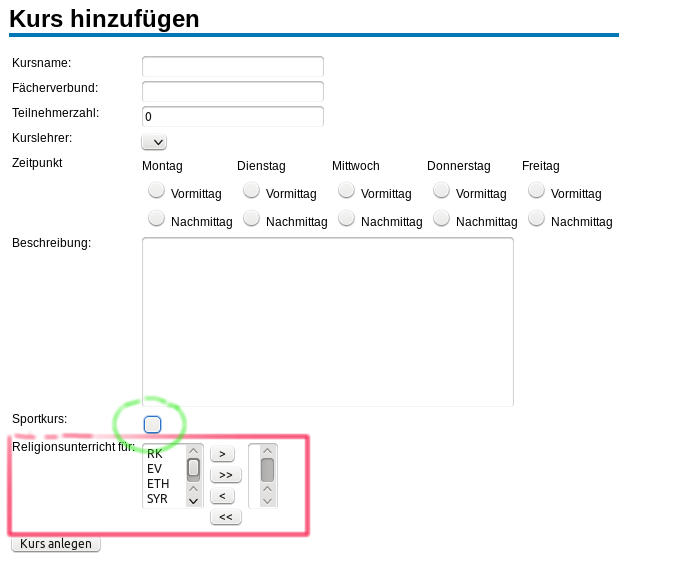
\includegraphics[scale=0.6]{img/KursAnlegen_KuWaSys.png}
 \end{center}
 \caption[\textbf{KuWaSys: Kurs anlegen}]{KuWaSys: Kurs anlegen}
 \label{fig:KursAnlegen_KuWaSys}
\end{figure}

\textbf{Pflichtkurse}

Ähnlich wie bei Sportkursen handelt es sich hierbei um ein Attribut, also ebenfalls einer Spalte in der Kurs-Tabelle, die auch den Datentyp \texttt{boolean} besitzt.
Im Gegesatz zu Sportkursen wird das Pflichtkurs-Flag allerdings nicht beim Anlegen eines Kurses gesetzt. Es kann nur vom Admin bestimmt werden, ob ein Kurs ein Pflichtkurs ist oder nicht. Festlegen kann er dies in der Kursverwaltung in der Phase der Kursplanung.

Die \prettyref{fig:KursVerwalten_KuWaSys} zeigt einen Ausschnitt der Kursverwaltung aus Sicht des Admins.
Der Admin hat die Möglichkeit Kurse zu aktivieren, also den Schülern die Kurse zur Kurswahl zur Verfügung zu stellen oder bereits aktivierte Kurse wieder zu deaktivieren.
Darüberhinaus legt der Admin die Pflichtkurse fest.

% Kurs verwalten
\begin{figure}[H]
 \begin{center}
   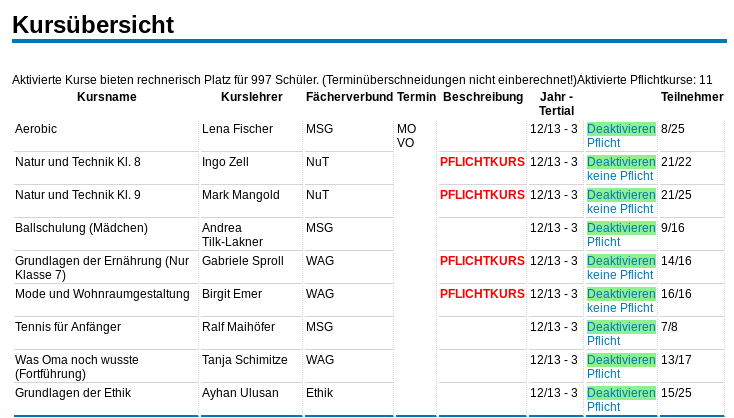
\includegraphics[scale=0.6]{img/KursVerwalten_KuWaSys.png}
 \end{center}
 \caption[\textbf{KuWaSys: Kurse verwalten}]{KuWaSys: Kurse verwalten}
 \label{fig:KursVerwalten_KuWaSys}
\end{figure}

\subsubsection{Benutzerunterstützung}
%%
\todo[size=\small, color=red!40]{Anzeige der abgehandelten Kurse/Fächerverbünde etc... (Schüler bzw. Admin)}
%%%%
\todo[size=\small, color=orange!40]{Screenshot}
%%


\subsection{Systemverwaltung}
%%
\todo[size=\small, color=red!40]{Umsetzung der Stati des Systems}
%%%%
\todo[size=\small, color=orange!40]{Screenshot}
%%



\section{Tests, Fehlervermeidung und Qualitätssicherung}\label{sec:Testing und Debugging}

%% Einleitung %(
Dieser Abschnitt widmet sich dem Thema der Testverfahren in Softwareprojekten mit dem Schwerpunkt bezogen auf das entwickelte JSF-Projekt 'KuWaSys'.
Zuerst sollen die allgemein geltenden Grundlagen angesprochen werden, darauf aufbauend werden die im Projekt verwendeten Testverfahren näher erläutert. 

Tests lassen sich in der Software Entwicklung nach ihrer Art und Weise klassifizieren.
Auf der einen Seite steht die Konstruktive-Qualitätssicherung auf der anderen Seite die Analytische.

Zu den Konstruktiven-Qualitätssicherungsmaßnahmen zählen Durchführungen während dem und am Entwicklungsprozesses selbst:
\begin{itemize}
  \item Checklisten
  \item Programmier-Guidlines
  \item Templates
\end{itemize}

Die Analytischen-Qualitätssicherung, zu welchen Tests am Produkt gehören, können in zwei verschiedene Testverfahren eingeteilt werden. Hierbei handelt es sich um statische und dynamische Tests.
Verfahren die hierzu eingesetzt werden sind für statische Test:
\begin{itemize}
  \item Statische Analyse
  \item Reviews
\end{itemize}

Im Sinne der statischen Analyse wurden während der Entwicklung folgende Punkte überprüft:
\begin{itemize}
  \item existieren Klassen bzw. Methoden
  \item sind die Scopes der ManagedBeans korrekt
  \item sind ManagedBeans mit dem Scope \texttt{Session} und \texttt{Application} serialisierbar
  \item haben ManagedBeans Properties die benötigten Setter-/Getter-Methoden
\end{itemize}

Und für dynamische Test beispielsweise:
\begin{itemize}
  \item \gls{Blackbox}-Testverfahren
  \item \gls{Whitebox}-Testverfahren
\end{itemize}


Die Planung und Strukturierung der Durchführung von Softwaretests, aber auch die Überlegung von Testfällen die am System geprüft werden sollen, stellen einen äußerst wichtigen Prozess der Softwareentwicklung dar.
Diese Schritte fließen bestenfalls zu Beginn des Projekts, in der Planungsphase, mit ein. (\cite{SPM}, ab Seite 5undzwölfzig)

%% TODO evtl hier checkliste?!
Als geplante Tests am fertigen System wurden die folgenden vorgesehen, die im Checklisten-Verfahren abgearbeitet wurden:
\begin{itemize}
	\item Tests bezügliche der Interaktion am System (mit Testpersonen und deren Feedback)
	\begin{itemize} 
		 \item prüfen der Übersichtlichkeit aller Benutzergruppen
		 \item Kontrolle des Seitenaufbaus und der Strukturierung für effizientes Arbeiten
	\end{itemize}
	\item Testeingaben in Textfelder
	\begin{itemize} 
		 \item Tests der Schnittstellen und der übergebenen Parameter nach Datentyp
		 \item Abklärung von eventuellen Encoding-Problemen
	\end{itemize}
	\item Funktionalitätstests aller Schaltflächen
	\begin{itemize} 
		 \item absichern von korrekten Systemereignissen bzw. -funktionen
		 \item Kontrolle der übergebenen Werte und Datentypen, um Fehlbelegungen auszuschließen
	\end{itemize}
	\item Konsistenz der Datenbank 
	\begin{itemize} 
		 \item Abfragen mit Hinblick auf Eindeutigkeit, bspw. bei \texttt{UNIQUE-Constraints} sowie \texttt{PRIMARY KEY-} und \texttt{FOREIGN KEY-Constraints}
		 \item Überprüfung der verwendeten Datentypen im System
	\end{itemize}
\end{itemize}

Im folgenden sollen Tests im Zusammenhang mit der Softwarequalitätssicherung und die Umsetzung im 'KuWaSys' näher betrachtet werden.

Der Stellenwert der Qualitätssicherung von Software hat in der heutigen Zeit einen so großen Stellenwert angenommen, dass es mittlerweile sogar ISO-Normen gibt, genauer gesagt die ISO-Norm 9126 - für Qualität in Software. Diese Norm enthält grundlegende Bestimmungen über Effizienz, Funktionalität, Zuverläsigkeit, Benutzbarkeit, Portabilität und Wartbarkeit. 
Die genauen Details der Definitionen werden hier nicht weiter erwähnt da diese über das Thema der Projektarbeit hinaus gehen würden. Eine gute und vollständige Zusammenfassung der gesamten Norm ist jedoch unter \cite{WikiISO9126} zu finden.

% ISO 9126 MindMap
\begin{figure}[H]
\centering\begin{tikzpicture}[mindmap,
  level 1 concept/.append style={level distance=130,sibling angle=30},
  extra concept/.append style={color=blue!50,text=black}]

\begin{scope}[mindmap, concept color=green, text=white]
\node [concept]at (-2,1) {ISO 9126}[clockwise from=-5]
    child [grow=10] {node [concept] (E) {Effizienz}}
    child {node [concept] (F) {Funktionali-tät}}
    child [grow=240] {node [concept] (E) {Zuverläsig-keit}}
    child [grow=110] {node [concept] (B) {Benutzbar-keit}}
    child [grow=60] {node [concept] (P) {Portabilität}}
    child [grow=280] {node [concept] (W) {Wartbarkeit}};
\end{scope}
\end{tikzpicture}
\caption[\textbf{ISO Norm 9126}]{ISO Norm 9126}
\label{fig:Projekt_Mindmap}
\end{figure}
%)

%% Test/Qualität im Projekt %(
Grundsätzlich wurden allgemein gültige Richtlinien und Code-Konventionen von JSF im Projekt umgesetzt. Dies erhöht zum eine die Übersichtlichkeit des gesamten Projekts und wirkt sich postiv auf die kooperierende Entwicklung aus. Dadurch werden gleichermaßen qualitätsichernde Maßnahmen ergriffen wie auch Fehleranfälligkeiten minimiert.  

Das Benutzen von Templates, welche während der Implementierungsphase eingesetzt wurden, stellt ebenfalls eine Technik dar, die zur Fehlervermeidung beiträgt. Das verwendete Design des 'KuWaSys' musste somit nur einmal definiert und getestet werden und konnte anschließend beliebig oft weiter verwendet werden ohne dabei das Risiko eingehen zu müssen dass das Design inkonsistent wird oder dass sich neue Fehler im Projekt einschleichen könnten. 

Um Laufzeittests durchzuführen wurden FacesMessages, über den entsprechenden Import der Klasse \texttt{javax.faces.application.FacesMessage} benutzt, die Gleichzeitig die Fehleranalyse mit Hilfe der Konsole erleichtern.
Ein Beispiel solcher Messages ist in \prettyref{lst:FacesMessages} dargestellt. Im Falle eines Fehlers würde der ausgeführte \texttt{Catch}-Block, über den benutzerdefinierten FacesMessages-Befehl, eine Ausgabe produzieren.
Nebenbei sei noch eine weitere Besonderheit in JSF angemerkt:
Während der Status 'Development' im  Projekt steht, welcher in der \texttt{POM.xml} festgelegt wird, werden Fehler für bestimmte Funktionen automatisch ausgegeben. Dies ist vor allem bei einem Release zu beachten und vorher abzuändern.

%% Listing: FacesMessages
	\lstinputlisting[label={lst:FacesMessages},
	caption={Debugging mit FacesMessages},
	frame=tlbr, 
	language=java, 
	breaklines=true, 
	numbers=left, 
	numberstyle=\tiny, 
	stepnumber=1, 
	numbersep=5pt, 
	basicstyle=\small\ttfamily,
	showstringspaces=true,
	keywordstyle=\bfseries\color{lila}, 
	tabsize=2,
	backgroundcolor=\color{lightgrey}]{listings/FacesMessages.java}
	
Wie in der folgenden \prettyref{figmin:SchulerImportieren_KuWaSys} zu erkennen ist, wird die Message während der Laufzeit ausgeführt, wie bei diesem missglückten Datei-Upload.

% Kurs anlegen
\begin{figure}[H]
 \begin{center}
   
\includegraphics[scale=0.8]{img/SchulerImportieren_KuWaSys.png}
 \end{center}
 \caption[\textbf{KuWaSys: Datei-Upload Fehler beim Schüler Importieren}]{KuWaSys: Datei-Upload Fehler beim Schüler Importieren}
 \label{figmin:SchulerImportieren_KuWaSys}
 \label{fig:SchulerImportieren_KuWaSys}
\end{figure}

Diese Tests erwiesen sich bei Datenbankabfragen als sehr hilfreich, da nicht erst aufwändige Oberflächen umgesetzt werden müssen um Fehler zu erkennen, sondern Daten sofort auf ihre Richtigkeit hin geprüft werden können.
Diese Fehler sind gleich zu Beginn der Implementierung aufgefallen, da es sich hier vor allem um Fehler die während der Modellierungs- beziehungsweise (bzw.) Designphase entstanden sind, handelt. Diese Fehler sind mit FacesMessages relativ schnell auszumachen und ebenso schnell korrigiert. Beispiele solcher Fehler sind:
\begin{itemize}
  \item falsche Überlegungen zu den Datentypen in der \ac{DB}
  \item schlecht definierte Schnittstellen
  \item Inkonsitenz im Design 
\end{itemize}

Eine weitere Möglichkeit, Fehler in einer Webapplikation zu entdecken ist das benutzen von selbstdefinierten Server-Logs.
Hierzu wurde von uns die Klasse \texttt{import java.util.logging.Logger} verwendet. Der \prettyref{lst:Logger} zeigt wie beispielsweise ein \texttt{Catch}-Block  mitgeloggt werden kann.

%% Listing: Logging
	\lstinputlisting[label={lst:Logger},
	caption={Server-Logging in JSF},
	frame=tlbr, 
	language=java, 
	breaklines=true, 
	numbers=left, 
	numberstyle=\tiny, 
	stepnumber=1, 
	numbersep=5pt, 
	basicstyle=\small\ttfamily,
	showstringspaces=true,
	keywordstyle=\bfseries\color{lila}, 
	tabsize=2,
	backgroundcolor=\color{lightgrey}]{listings/Logger.java}

Da ständig auf einem aktiven System (Corporate Identity) - glossarntwickelt und getestet wurde konnten Tester aus dem Umfeld der Schule für diesen Zweck eingesetzt werden.
Dies erwies sich vor allem beim Entwickeln des Oberflächendesigns als Vorteil. Es konnten Wünsche von Lehrern und Schülern direkt berücksichtigt und umgesetzt werden.
Hier bekommen besonders Checklisten und Reviews einen hohen Stellenwert. Nur durch regelmäßige gemeinsame Treffen konnten Projekttermine (neu-)definiert werden.

Im Hinblick auf die vorher besprochene ISO-Norm 9126 erfüllt das Kurswahlsystem alle Bestimmungen. Jedoch muss fairnesshalber dazu gesagt werden, dass Dinge wie Effizienz in Software nie mit einem genauen Maß gemessen werden kann, da viele Faktoren ein Rolle spielen.
Zum Beispiel müssen bei gewissen Datenstrukturen Laufzeiteinschränkungen in Kauf genommen werden wenn sich dadurch die Darstellung effizienter umsetzen lässt. Andererseits können natürlich schneller Datenstrukturen oder Algorithmen in einer viel langsameren Darstellung resultieren.
Dasselbe gilt für die Zuverläsigkeit. Natürlich ist das Kurswahlsystem so entworfen worden, dass die Erreichbarkeit und Nutzbarkeit jederzeit gegeben ist. Aber auch hier unterliegt das System mehreren außenstehenden Faktoren auf die ein Entwickler niemals Einfluss nehmen kann.
%)

%% JSFUnit %(
Selbstverständlich können für den Java Server Faces Standard auch Tests implementiert werden. Diese werden für gewöhnlich bei den Dynamischen-Test angesiedelt. Von uns wurden keine spezielle Frameworks zur Realisierung von Tests verwendet. Vollständigkeitshalber soll allerdings eines der interessantesten Vertreter von Testinstrumenten für JSF erwähnt werden:

Hierbei handelt es sich um \gls{JSFUnit}, welches auf dem bekannten JAVA-Testframework \gls{JUnit} aufbaut. Tests können hierzu über die JSFUnit-Konsole oder durch den Aufruf einer Testseite ausgeführt werden. Testmöglichkeiten sind Wert- und Zustandsänderungen in ManagedBeans, setzen von Navigationszielen oder über FacesMessages.
Eine besondere Art der Tests sind die 'Acrylic Box'-Testings. Diese verbinden Whitebox und Blackbox-Testverfahren und werden bei den dynamischen Tests eingestuft.
Nähere Informationen sind unter \cite{JSFUnit01} zu finden.
%)

Zuletzt soll noch hinzugefügt werden, dass auch ausführliche Tests keine Garantie auf eine vollständige Fehlerfreiheit geben.
Allerdings helfen Tests die Fehler möglichst gering zu halten und steigern die Qualität der Software um ein gewisses Maß.
Obwohl das Projekt ausführlichst getestet wurde kann es dennoch nicht ausgeschlossen werden, dass noch welche existieren. 

\newpage

\section{Fazit und Ausblick}\label{sec:Fazit und Ausblick}

%% Einleitung %(
Abschließend soll ein gesamtheitlicher Überblick der Projektarbeit gegeben werden, indem das entwickelte System komplett betrachtet wird.
Für ein sinnvolles Fazit sollen zwei wesentliche Punkte angesprochen werden:
\begin{enumerate}
  \item Beurteilung der Nutzbarkeit und die gesamtheitliche Umsetzung des Projekts
  \item Beurteilung der eingesetzten Technologien
\end{enumerate}

%%% TODO
Vor allem beim zweiten Punkt sollen zwei weitere Kriterien differenziert werden:
Beim Einen handelt es sich um das Kriterium der Verwendbarkeit der Technologie für den Entwickler, hier ist dieser in einer aktiven Rolle zu sehen. 
Beim Anderen handelt es sich vor allem um eine Betrachtung der Technologie in Punkten wie Komplexität, Verwendbarkeit und Spezifiktaion, in welchen der Entwickler lediglich nur eine passive Rolle einnehmen kann.
%)

%% Betrachtung System %(
An oberster Stelle stand das Ziel, die Anforderungen an das System erfolgreich umzusetzen.
Das positive Resultat kann der engen Kooperation während der Implementierungsphase und der ausgiebigen Problemabgrenzung, wie grob zu Beginn in \prettyref{subsec:Problemstellung und -abgrenzung} beschrieben ist, angerechnet werden.
Vor allem die ersten drei bis vier Wochen nach Projektstart dienten dazu, die Ziele zu definieren. Beinahe jede Woche hielten wir mit den verantwortlichen Personen (in \prettyref{subsec:Verantwortliche Personen} namentlich aufgeführt) der Schillerschule Aalen ein Projektmeeting ab, in welchem Ergebnisse des Projektfortschritts präsentiert und diskutiert wurden.
Ein weiterer wichtiger Punkt, der zu diesem Ergebnis geführt hat, war das entgegengebrachte Vertrauen von Seiten der Schule.

Wie es \prettyref{secmin:Implementierung} zu entnehmen ist, wurden alle Punkte der Systemanforderung erfüllt. Darüberhinaus wurden sogar zusätzliche Funktionalitäten implementiert.
Hier wäre die Umsetzung der Export-/Importfunktionen von CSV Dateien, Funktionalität die Userdaten betreffen (bspw. Passwort-Neugenerierung) und die komplette Umsetzung der \ac{IT}-Infrastruktur der Schillerschule genannt. 
Insofern muss der entstandene Fortschritt mit dem neuen Kurswahlsystem im Hinblick auf das erste Kursverwaltungstool gesehen werden.

Das größte Manko, der nicht unterstützte Multi-User Betrieb und die Einschränkung der Lauffähigkeit begrenzt auf ein System, wurden beseitigt. Ebenso wurde mehr Wert auf ein gewisses Maß an Selbstverantwortung bei Lehrern aber auch Schülern gelegt.
Im Idealfall wird der Admin nur noch zur Konfiguration des Systems und in Problemfällen aktiv.
Auch die Verwaltungsassistenz wurde im neuen Tool erfolgreich umgesetzt. So werden Daten die für die Kursplanung wichtig sind vom System ermittelt und den Benutzern zur Verfügung gestellt. 
Ebenso wurde der entwickelte Arbeitsablauf für Lehrer und Schüler umgesetzt und die Kommunikation untereinander dadruch verbessert indem Probleme Systembedingt abgefangen werden können.

Als dritter und letzter Verbesserungsschritt ist die neugestaltung der Oberfläche zu sehen. Diese wurden mit Hilfe von bereits erprobten und bewährten Gestaltungselementen, die aus dem Gebiet der \ac{MCI} bekannt sind, umgesetzt. \cite{DahmMCI}.

Die eindeutige Abgrenzung von Menü, Informationen und Arbeitsbereich sind gleichermaßen umgesetzt wie die Darstellung aller Systemrelevanter Daten wie es in der Anforderung gewünscht war.

Zukünftige Erweiterungen sind im System vorgesehen. Aufgrund der Modularität die sich strikt durch das ganze System zieht werden diese auch realisierbar sein.

Realisierbare Erweiterungen könnten sein:
\begin{itemize}
  \item eine Änderungsinformationsanzeige für Admins bei bestimmten Systemereignissen, sodass ohne fundierte \ac{IT}-Kenntnisse, Fehler an Server und Datenbank frühzeitig erkannt werden können
  \item eine interne Kommunikationsplattform für den Austausch von Informationen zwischen Lehrern und Administrator und zwischen Schülern - und Lehrern  
  \item Erweiterungen wie Kalenderfunktionen, Stundenplan-Generierung,....
\end{itemize}
  
Manche der aufgeführten Vorschläge werden bereits im Momentanen Stand der Entwicklung, ansatzweise umgesetzt. 
Aufgrund der Fülle und Diversität der Art an Anforderungen die zu Beginn an das Projekt festgehalten wurden fanden diese jedoch in der Projektarbeit bedauerlicherweise fast keinen Platz.
%)

%% Technologien %(
Es hat sich gezeigt, dass \ac{JSF} ein gut definierter Webentwicklungsstandard geworden ist.
Aufgrund der Einfachheit der Handhabung kommen Anfänger der Webentwicklung aber auch Fortgeschrittene gut damit zurecht und voll auf ihre Kosten.
Je nach Komplexität der Interaktion mit dem System sind JAVA Kenntnisse erfoderlich, in jedem Falle aber sinnvoll. 
Eine Entwicklung die ihren Schwerpunkt auf das Design oder generell die Darstellung legt benötigt nur sehr wenige Kenntnisse im Bereich JAVA dafür aber Kenntnisse einer Seitendeklarationssprache wie HTML oder JSP.
Sollen aber, wie es in dieser Projektarbeit der Fall war, Daten aus einer Datenbank verändert oder in eine Datenbank geschrieben werden sind fundierte Kenntnisse der Softwareentwicklung mit JAVA notwendig.

Zur verwendeten Datenbank lassen sich keine besonders wichtigen oder bahnbrechenden Aussagen machen. PostgreSQL hat sich bereits über Jahre etabliert und wurde stetig weiter verbessert. 
Die Verwendung für unerfahrene Nutzer stellt nach einer kurzen Einarbeitung kein größeres Problem dar und kann somit nur weiterempfohlen werden. 
 
Die Entwicklungsunterstützung mit Maven ist bei Projekten dieser Art eine sehr große Hilfe.
Ohne eine Verwaltungshilfe der Bibliotheken, Pakete oder der Projektverweise kann ein Projekt in dieser Größenordnung schnell in einen Bereich kommen, in welchem plötzlich der Verwaltungsaufwand steigt und schnell zur Hauptaufgabe des Entwicklers wird.
Der Fokus schweift immer öfters vom Projekt ab. Das Resultat davon ist:
\begin{itemize}
	\item ein höherem Zeitaufwand für das Beheben von entstandenen Problemen durch die Verletzung von Abhängigkeiten 
	\item mehr Fehler im Programmcode der wiederrum auch zu längeren Testphasen führt
	\item teilweise leidet die Qualität des entstanden Codes 
\end{itemize}
Für viele Entwickler (oder Projektleiter) ist dies ein stark vernachlässigtes Thema.
Ohne eine genaue Planung und ohne konkrete Vorstellungen lässt sich jedoch ein Softwareprojekt, egal welcher Größe, meist nie korrekt realisieren.  
Dies sind alles Gründe die dafür gesorgt haben, dass das Projekt unter zu Hilfenahme des Development-Tools Maven umgesetzt wurde.
Die Softwareentwicklung bleibt im Vordergrund.
%)

%% Rückblick %(
Rückblickend kann dem Projekt ein voller Erfolg zugeschrieben werden.
Funktional genügt das System den Anforderungen und sogar darüber hinaus. Der zeitliche Aufwand war sehr hoch, aber im Rahmen des Möglichen, sodass nicht von 'zu viel' gesprochen werden kann.
Zeitliche Einbußen musste dennoch hingenommen werden. So stellten vor allem das Testen und die Integration des Systems in die Infratruktur der Schule einen langwierigen Prozess dar und sprengte den geplanten Rahmen.
Letztenendes sorgten Dinge wie die Anleitung, die technische Dokumentation und diese Ausarbeitung der Projektarbeit für den nötigen Abschluss des Projekts.

%)

\newpage

%% Neuer Style
\pagestyle{fancy}
	\renewcommand{\sectionmark}[1]{\markboth{#1}{}}
	\fancyhf{}
	\fancyhead[L]{ { }\leftmark}
	\fancyhead[R]{\thepage}
	\renewcommand{\headrulewidth}{0.4pt}
	%\pagenumbering{roman}

Die ist in \prettyref{sec:Anhang} zu finden.
	
\begin{appendix}
\section{Anhang}\label{sec:Anhang}

\subsection{Inhalte der CD}
Folgende Inhalte sind auf der abgegebenen CD zu finden:

\begin{itemize}
  \item Kopie der Entwicklungsumgebung Eclipse 10.04 Juno mit allen Plugins
  \item virtuelles Abbild des konfigurierten Servers
  \item diese Ausarbeitung
  \item Dokumentation in JAVAdoc
  \item Benutzerhandbuch für das 'KuWaSys'				%%
  \item Kopien der verwendeten bzw. zitierten Websites\todo[size=\small, color=green!40]{Fragwürdig!!!} 
\end{itemize}											%%

\subsection{Konfiguration und Installation}

\subsubsection{Maven}

Maven Befehle listings

\subsubsection{Apache Tomcat 7}

Hier soll in einer kurzen Darstellung die Administration des Apache Tomcat 7 und dessen wichtige Dateien und Verzeichnisse 

\textbf{}
Apache Tomat7 Befehle Listings

Verzeichnisse

\subsection{Zugangsdaten für den Server und das System}

\textbf{Server Zugangsdaten}

% Zugangsdaten
\begin{table}[H]
\begin{center}
	\begin{tabular}{|l|l|l||}\hline
		\textbf{Rolle} & \textbf{Username} & \textbf{Passwort} \\ \hline
		Admin & ijcy & 12kuwasys34 \\ \hline \hline
	\end{tabular}
	\caption{Server Zugangsdaten}
\end{center}
\end{table}

\textbf{Datenbank Zugangsdaten}

% Datenbank Zugangsdaten
\begin{table}[H]
\begin{center}
	\begin{tabular}{|l|l|l||}\hline
		\textbf{Rolle} & \textbf{Username} & \textbf{Passwort} \\ \hline
		Admin & ijcy & 12kuwasys34 \\ \hline
		Admin & postgres & 12kuwasys34 \\ \hline \hline
	\end{tabular}
	\caption{Datenbank Zugangsdaten}
\end{center}
\end{table}

\subsection{Gesetzesauszüge}\label{subsec:Gesetz}

Auszug aus dem \ac{TMG}:

\textbf{§ 5 Allgemeine Informationspflichten}
\begin{itemize}
\item[(1)] Diensteanbieter haben für geschäftsmäßige, in der Regel gegen Entgelt angebotene Telemedien folgende Informationen leicht erkennbar, unmittelbar erreichbar und ständig verfügbar zu halten:
  \begin{enumerate}
    \item den Namen und die Anschrift, unter der sie niedergelassen sind, bei juristischen Personen zusätzlich die Rechtsform, den Vertretungsberechtigten und, sofern Angaben über das Kapital der Gesellschaft gemacht werden, das Stamm- oder Grundkapital sowie, wenn nicht alle in Geld zu leistenden Einlagen eingezahlt sind, der Gesamtbetrag der ausstehenden Einlagen,
    \item Angaben, die eine schnelle elektronische Kontaktaufnahme und unmittelbare Kommunikation mit ihnen ermöglichen, einschließlich der Adresse der elektronischen Post,
    \item soweit der Dienst im Rahmen einer Tätigkeit angeboten oder erbracht wird, die der behördlichen Zulassung bedarf, Angaben zur zuständigen Aufsichtsbehörde,
    \item das Handelsregister, Vereinsregister, Partnerschaftsregister oder Genossenschaftsregister, in das sie eingetragen sind, und die entsprechende Registernummer,
    \item soweit der Dienst in Ausübung eines Berufs im Sinne von Artikel 1 Buchstabe d der Richtlinie 89/48/EWG des Rates vom 21. Dezember 1988 über eine allgemeine Regelung zur Anerkennung der Hochschuldiplome, die eine mindestens dreijährige Berufsausbildung abschließen (ABl. EG Nr. L 19 S. 16), oder im Sinne von Artikel 1 Buchstabe f der Richtlinie 92/51/EWG des Rates vom 18. Juni 1992 über eine zweite allgemeine Regelung zur Anerkennung beruflicher Befähigungsnachweise in Ergänzung zur Richtlinie 89/48/EWG (ABl. EG Nr. L 209 S. 25, 1995 Nr. L 17 S. 20), zuletzt geändert durch die Richtlinie 97/38/EG der Kommission vom 20. Juni 1997 (ABl. EG Nr. L 184 S. 31), angeboten oder erbracht wird, Angaben über
    \begin{itemize}
      \item[a)] die Kammer, welcher die Diensteanbieter angehören,
      \item[b)] die gesetzliche Berufsbezeichnung und den Staat, in dem die Berufsbezeichnung verliehen worden ist,
      \item[c)] die Bezeichnung der berufsrechtlichen Regelungen und dazu, wie diese zugänglich sind,
    \end{itemize}
    \item in Fällen, in denen sie eine Umsatzsteueridentifikationsnummer nach § 27a des Umsatzsteuergesetzes oder eine Wirtschafts-Identifikationsnummer nach § 139c der Abgabenordnung besitzen, die Angabe dieser Nummer,
    \item bei Aktiengesellschaften, Kommanditgesellschaften auf Aktien und Gesellschaften mit beschränkter Haftung, die sich in Abwicklung oder Liquidation befinden, die Angabe hierüber.
  \end{enumerate}
\item[(2)] Weitergehende Informationspflichten nach anderen Rechtsvorschriften bleiben unberührt.
\end{itemize}

Auszug aus dem \ac{RstV}:

\textbf{§ 55 - Informationspflichten und Informationsrechte}
\begin{itemize}
  \item[(1)] Anbieter von Telemedien, die nicht ausschließlich persönlichen oder familiären Zwecken dienen, haben folgende Informationen leicht erkennbar, unmittelbar erreichbar und ständig verfügbar zu halten:
  \begin{enumerate}
    \item Namen und Anschrift sowie
    \item bei juristischen Personen auch Namen und Anschrift des Vertretungsberechtigten.
  \end{enumerate}
  \item[(2)] Anbieter von Telemedien mit journalistisch-redaktionell gestalteten Angeboten, in denen insbesondere vollständig oder teilweise Inhalte periodischer Druckerzeugnisse in Text oder Bild wiedergegeben werden, haben zusätzlich zu den Angaben nach §§ 5 und 6 des Telemediengesetzes einen Verantwortlichen mit Angabe des Namens und der Anschrift zu benennen. Werden mehrere Verantwortliche benannt, so ist kenntlich zu machen, für welchen Teil des Dienstes der jeweils Benannte verantwortlich ist. Als Verantwortlicher darf nur benannt werden, wer
  \begin{enumerate}
    \item seinen ständigen Aufenthalt im Inland hat,
    \item nicht infolge Richterspruchs die Fähigkeit zur Bekleidung öffentlicher Ämter verloren hat,
    \item voll geschäftsfähig ist und
    \item unbeschränkt strafrechtlich verfolgt werden kann.
  \end{enumerate}
  \item[(3)] Für Anbieter von Telemedien nach Absatz 2 Satz 1 gilt § 9 a entsprechend.
\end{itemize}

\subsection{Verantwortliche Personen}\label{subsec:Verantwortliche Personen}

Ralf Meiser - Konrektor

Björn Bolch - 

Alexander Neugebauer - IT Systembeauftragter der Schillerschule Aalen

%% Abkürzungsverzeichnis
\newpage
\section{Akronyme}
\input{PA-01-Projekt_PDFVersion_KuWaSys.acronym}

%% Glossar

\newpage
\section{Glossar}
\glossary{
  name={entry name}, 
  description={entry description}
}
\printglossary[title={}] 

\end{appendix}

% Abbildungsverzeichnis
\newpage
\addcontentsline{toc}{section}{\textbf{Abbildungsverzeichnis}}
\listoffigures
\cleardoublepage

% Tabellenverzeichnis
\newpage
\addcontentsline{toc}{section}{\textbf{Tabellenverzeichnis}}
\listoftables
\cleardoublepage

% Quellcodeverzeichnis
\newpage
\addcontentsline{toc}{section}{\textbf{Quellcodeverzeichnis}}
\lstlistoflistings
\cleardoublepage

%% Literaturverzeichnis
\newpage
\addcontentsline{toc}{section}{\textbf{Literaturverzeichnis}}
\bibliographystyle{alphadin}	  
\bibliography{PA-01-Projekt_PDFVersion_KuWaSys}

%% Eidesstattliche Erklärung
\addcontentsline{toc}{section}{\textbf{Eidesstattliche Erklärung}}

\end{document} 


\makeglossaries
\begin{document}
	\parindent0ex
	\parskip2ex
	
	%% TODO
	\listoftodos
	\newpage
	
	\pagestyle{empty}
	\maketitle
	\thispagestyle{empty}
	\cleardoublepage
	\newpage
	
	\vspace{10cm}
	\section*{Zusammenfassung}
	
	\pagestyle{fancy}
	\renewcommand{\sectionmark}[1]{\markboth{#1}{}}
	\fancyhf{}
	\fancyhead[L]{ { }\leftmark}
	\fancyhead[R]{\thepage}
	\renewcommand{\headrulewidth}{0.4pt}
	\pagenumbering{roman}
	
	
Diese Projektarbeit beschäftigt sich mit dem Thema der Modellierung und Implementierung 
eines Kurswahlsystems für eine Werksrealschule.

Die Modellierung beschäftigte sich vor allem mit dem Erarbeiten von Lösungsansätzen zur Datenhaltung und Umsetzungen in den Webtechnologien.

Das Resultat der Implementierung des Projekts war eine Webanwendung welche mit Hilfe des Apache Webstandards, den Java Server Faces
umgesetzt wurde.
Ferner wurde eine komplette Laufzeitumgebung für die bereits bestehende Infrastruktur der Schule erarbeitet und eingerichtet.
	\cleardoublepage
	
	% Inhaltsverzeichnis 
	\newpage
	\tableofcontents
	\cleardoublepage
	
	\printnomenclature
	\cleardoublepage
	\pagestyle{fancy}
	\renewcommand{\sectionmark}[1]{\markboth{#1}{}}
	\fancyhf{}
	\fancyhead[EL]{\thesection { }\leftmark}
	\fancyhead[OR]{{ }\rightmark}
	\renewcommand{\headrulewidth}{0.4pt}
	\pagenumbering{arabic}
	
% 	\fancyfoot[ER]{\textit{KuWaSys}}
% 	\fancyfoot[OL]{\textit{KuWaSys}} 
%   
  	\fancyfoot[EL]{\textbf{\thepage}}
	\fancyfoot[OR]{\textbf{\thepage}} 
% 	
% 	\renewcommand{\footrulewidth}{0.8pt}
	
	\setcounter{page}{1}

%% Einleitung X
\section{Einleitung}

\subsection{Motivation}

Im Sinne unserer Medien-Projektarbeit haben wir ein webbasiertes System zur Kurswahl und Kursverwaltung der Aalener Werksrealschule \iz{'Schillerschule'}{\url{http://www.schillerschule-aalen.de}} realisiert.

Ein kurzes Portrait der Schillerschule: (entnommen aus \cite{Sch-Po})

\begin{center}
\textit{
\grqq Die Schillerschule ist eine städtische Ganztagesschule mit rund 500 Schülerinnen und Schülern. Die Entwicklung zu einem Lern- und Lebensraum kennzeichnet das Profil der Schule. Wesentliche Ziele sind die Förderung von Lernen und Leistung sowie die kulturelle und gesellschaftliche Integration der Kinder und Jugendlichen mit ihren unterschiedlichen Herkunfts- und Erfahrungshorizonten.\glqq}
\end{center}

Wichtig war es, dass das Kurswahlsystem von verschiedenen Benutzern, wie Schülern sowie Lehrern, von überall aus zugänglich ist und außerdem später von einem Administrator verwaltet werden kann. Ferner sollte das gesamte Kurswahlmanagment über das neue Tool 'KuWaSys' erfolgen.

Die Realisierung des Systems wurde serverseitig mit einem \gls{Apache Tomcat} und \gls{Java Server Faces}, genauer mit einer Implementierung der \ac{JSF} namens \gls{JSF-myFaces Core} 2.1 und \gls{JSF-myFaces Tomahawk} in der Version 2.0, umgesetzt.
Die Zugänglichkeit auf der Seite der Clients konnte somit über jeden beliebigen Webbrowser realisiert werden.

Die benötigte Haltung der Daten sowie deren Bereitstellung wurde mit einer PostgreSQL \ac{DB} für das gesamte System umgesetzt.

Das \gls{User Interface} wurde mit \gls{HTML}, genauer gesagt mit HTML 5 umgesetzt. Der HTML Code wurde nicht wie es in der serverseitigen Programmierung üblich ist in \ac{JSF}-Dateien eingebettet, sondern in eigenständige HTML Dateien.
Diese werden in der \ac{JSF}-Technologie kurz: 'Facelets' genannt.

\subsection{Problemstellung und -abgrenzung}\label{subsec:Problemstellung und -abgrenzung}

Die Schillerschule hat bereits ein 'in die Jahre gekommenes' Tool zur Realisierung der Kurswahlen von Schülern, das bis dahin genannte 'KuhWa-Tool'. Ebenso wird momentan die Verwaltung der Kurse, von Lehrern der Schule über dieses Tool abgewickelt.
Die Schwierigkeiten welche durch das alte Tool entstanden sind können aufgrund ihrer Beschaffenheit in zwei grundlegende Kategorien eingeteilt werden:

Das umständliche und nicht intuitive gestaltete \ac{UI} auf der einen Seite, die mitlerweile überholte Programmstruktur mit diverser mangelhafter Funktionalität auf der Anderen.
Die Bedienung des Tools erweißt sich als nicht mehr praktikabel, da es erstens kompliziert zu verwalten ist und nur geschultes Lehrpersonal es bedienen kann, zweitens ist das Kurswahlsystem nur auf einer Laufzeitumgebung der Schule problemlos lauffähig und einsetzbar.
Probleme die auf die Funktionalität der Software zurückzuführen sind und darüber hinaus für die Schule einen weitaus größeren Mehraufwand bedeuteten, haben jedoch ein weitaus größere Bedeutung für die Kurswahl der Schule, wie nur das umständlich zu bedienende Design.

Das alte Tool hat keine Möglichkeiten für die Benutzerdatenverwaltung der Schüler und Lehrer der Schule. Änderungen sind schwer wieder rückgängig zu machen, Systemänderungen teilweise garnicht.
Ein Mehrbenutzerbetrieb ist weder für Kurswahlen noch für die Verwaltung möglich.
Ein einheitliches Konzept für die \ac{DB} ist ebenso nicht vorhanden.
Bei der bisher verwendeten \ac{DB} handelt es sich bisher um eine lokal angelegte \gls{Microsoft Access Datenbank}. Der Zugriff auf diese ist also auch nur systemweit möglich.

\subsection{Über diese Ausarbeitung}\label{subsec:Uber diese Ausarbeitung}

\textbf{Sinn und Zweck dieser Ausarbeitung}

Es soll zu Beginn erwähnt werden, dass diese Ausarbeitung nicht als eine Anleitung oder eine vollständige Dokumentation unserer Implementierung verstanden werden soll. Wobei der zweite Punkt treffender wäre. Wir wollen vor allem Einblicke in die Arbeit mit \ac{JSF}, der dazugehörigen Umgebung und die Umsetzung eines Projekts der \ac{IT} dieser Größenordnung geben. Ferner wollen wir einen strukturierten und nachvollziehbaren Verlauf unserer Entwicklungen darstellen.

Die Dokumentation des in \gls{JAVA} geschriebenen Codes unserer Arbeit ist ausführlich als \gls{JAVAdoc} vorhanden und dokumentiert. Für die Benutzung des System gibt es ein ausführliches Benutzerhandbuch, welches vor der Arbeit mit dem System um größere Schäden zu vermeiden unbedingt gelesen werden sollte. Die Konfiguration der Laufzeitumgebung (Netzwerk und Webserver) und die Implementierung der \ac{DB} kann in dieser Arbeit als vollständig dargestellt angesehen werden.

\textbf{Aufbau dieser Ausarbeitung}

Diese Ausarbeitung gliedert sich in drei große Teile. An erster Stelle befinden sich die Grundlagen welche in \prettyref{sec:Grundlagen} zu finden sind, welche für das Design und die Implementierung des neuen System nötig waren.
Im wesentlichen Dinge, die für die Einrichtung einer einwandfreie Entwicklungsumgebung gemacht wurden. Außerdem sollen grundlegende Einblicke in die \ac{JSF} sowie die \ac{DB}-Entwicklung gegeben werden.

Der zweite Teil beschäftigt sich mit der eigentlichen Modellierung (in \prettyref{sec:Modellierung}) des Systems, der dritte Teil mit der eigentlichen Implementierung (in \prettyref{sec:Implementierung}). In beiden Teilen sollen die wichtigsten und für dieses Projekt relevante Themen, Elemente und Inhalte näher besprochen werden.

Das methodische Konzept dieser Ausarbeitung ist immer von einfachen zu komplexen und von bekannten zu unbekannten Inhalten gegliedert. Dem Leser werden immer wieder neue Problematiken aufgezeigt und anhand von bekannten Lösungsansätzen anschaulich erklärt. Auch im Aufbau der Arbeit soll ein 'roter Faden' zu erkennen sein. So wird eine Beschreibung zu einer bestehenden Problematik und deren Lösungsansatz immer in die verschiedenen Rollen des System aufgeteilt und gesondert behandelt.  
\newpage

%% X
\section{Grundlagen}\label{sec:Grundlagen}

Wie schon in \prettyref{subsec:Uber diese Ausarbeitung} erwähnt, sollen in diesem Abschnitt der Ausarbeitung die Grundlagen der von uns verwendeten Technologien angesprochen und näher erläutert werden. Zu Begin wird der Teil der unterstützenden Tools besprochen. Anschließend grundlegende Kenntnisse der von uns konfigurierten Laufzeitumgebung bis hin zur Webentwicklung mit \ac{JSF}.


\subsection{Eclipse und Enwticklungsunterstützung}
Umfangreiche Softwareprojekte lassen sich durch die Verwendung einer \gls{Integrated Development Environment} (IDE) wie \gls{Eclipse} oder \gls{NetBeans} besser bearbeiten. 
Eclipse wurde ursprünglich von IBM entwickelt und im Jahr 2001 quelloffen veröffentlicht. Im Jahre 2004 übernahm die \gls{Eclipse-Foundation} die Weiterentwicklung des Projekts und ist heute neben der gls{Apache Software Foundation} eines der größten Open-Source-Communities im Bereich der JAVA-Softwareentwicklung.
Seit dem Jahr 2006 wurden verschiedene Versionen und Unter-Projekte von Eclipse auf einen gemeinsamen und aktuellen Stand gebracht.
Nach vielen Jahren der Entwicklung und stetigen Verbesserungen ist Eclipse heutzutage eines der beliebtesten IDEs im Bereich der Anwendungsentwicklung.
Heute ist Eclipse weit entfernt davon eine IDE nur für JAVA zu sein. Diverse Erweiterungen machten es zum dem Entwicklungstool für Software jedglicher Art und beinahe jeglicher Programmiersprache, schlechthin.

Für die Entwicklung des Projekts selbst wurde die \textit{Version 4.2 Juno} verwendet.
Außer den Basisfunktionen stehen Entwicklern viele Möglichkeiten offen diverse Plug-ins und Tools zu verwenden, die die Arbeit erleichtern.

Die für dieses Projekt verwendeten Softwareunterstützungen, waren:
\begin{itemize}
	\item \gls{Apache Maven}
	\item Eclipse WTP
	\item JBoss-Tools
	\item Git-Repository
\end{itemize}
  
Juno selbst stellt standardmäsig bereits über die Enterprise Edition, das Projekt \ac{WTP}, eine Unterstützung für die Entwicklung von JSF bereit. 
Eine weiteres Tool, die \gls{JBoss}-Tools, welche auch eine Erweiterung der Entwicklungsunterstützung im aktuellen Projekt darstellen, werden im übernächsten Unterabschnitt noch genauer erklärt.

Zur Automatisierung einzelner Schritte in der Softwareentwicklung wurde das Build- und Management-Tool Apache Maven zur Umsetzung verwendet. 

Desweiteren kam die freie Software zu Versionsverwaltung \gls{Git} zum Einsatz. Software dieser Art bietet sich vorallem bei kollaborativen Projekten, also Projekten mit mehreren Entwicklern an. 
Aber auch der Vorteil der Versionskontrolle bei kleinen 'Ein-Mann-Projekten' soll besser nicht unterschätzt werden.           
	 
Im folgenden soll zuerst jedoch auf Maven eingegangen werden.
\subsection{Apache Maven}

Der sinnvollste Weg ein \ac{JSF} Projekt zu verwalten ist Apache Maven.
Das Tool wird von der \gls{Apache Software Foundation} entwickelt und dient zur Verwaltung von Softwareprojekten überwiegend im JAVA Umfeld. In einer \gls{XML}-Struktur, dem \ac{POM}, wird das Projekt beschrieben und die notwendigen Angaben zur Erstellung einer lauffähigen Version vorgehalten. Darunter finden sich unter anderem Informationen über die Art des Projekts (im Sinne dieses Projekts waren es ein JSF-myFaces Core Projekt), Angaben zur Art des Erstellvorgangs und Abhängigkeiten wie z.B. der JSF-myFaces Core-\gls{API}, JSF-myFaces Tomahawk, und \gls{PostgreSQL}.

Für die Entwicklung und Integration von Maven in \gls{Eclipse} bietet sich die Installation ds Plug-ins \textit{m2e} bzw. \textit{m2eclipse} an. Die Integration und Verwendung von Maven in Eclipse ist unter \cite{EclM2E} näher beschrieben. 
Bei Maven steht vorallem die Integration der Webapp sowie die Bibliotheks- und Versionsverwaltung im Vordergrund. 
Das erstellte \gls{Apache Maven}-Projekt kann somit in Eclipse importiert und dort bearbeitet werden oder wird schon zu Beginn in Eclipse angelegt. 
Eine Integration von \gls{Apache Tomcat} in Eclipse bietet dann die Möglichkeit die Webapp ohne umständliches Erstellen und Installieren auf dem \gls{Servlet-Container} zu verwenden.

% Maven Workflow
\begin{wrapfigure}[12]{r}{12cm}
\centering\begin{tikzpicture}[decoration=penciline, decorate]
  \node at (1,4) {Projekt Workspace};
  \node at (8,4) {Maven Repository};

  % Repo
  \draw[dashed, decorate,ultra thick] (0,-1) -- (0,3) -- (3,3) -- (3,-1) -- (0,-1);
  \draw[draw=black, fill=yellow!30!, opacity=0.4, decorate,thick] (1,1) -- (1,2.8) -- (2.8,2.8) -- (2.8,1) -- (1,1);
  \node[decorate] at (1.9, 2.5) {$POM$};
  \node[decorate] at (1, 0) {$/lib/$};

  % Pfeil
  \draw[->, color=black, out=50, in=190, thick] (2,2) to (8,2.5);
  \draw[->, color=black, out=20, in=170, thick] (2.8,0) to (8,1.5);

  % Libs
  \node[decorate, circle, fill, red, inner sep=4pt] at (2.3,-0.2) {};
  \node[decorate, circle, fill, red!20!, inner sep=4pt] at (2.1,0.2) {};
  \node[decorate, circle, fill, red!50!, inner sep=4pt] at (2,-0.5) {};
  \node[decorate, circle, fill, blue!60!, inner sep=4pt] at (1.8,-0.2) {};

  % Pfeil
  \draw[decorate, <-, color=black!50!white, out=270, in=180, thick] (1,-0.2) to (2,-1.6);
  \node[decorate] at (2,-1.8) {\textit{\small{...internes lib-Verzeichnis}}};

  % Maven Repo
  \draw[very thick] (8,2.5) ellipse (60pt and 20pt);
  \draw[very thick] (8,0) ellipse (60pt and 20pt);
  \draw[decorate, very thick] (6,0) -- (6,2.5);
  \draw[decorate, very thick] (10,0) -- (10,2.5);
\end{tikzpicture}
\caption[\textbf{Maven Verwaltung}]{Skizze der Maven Verwaltung}
\label{fig:Maven_Verwaltung}
\end{wrapfigure}

In \prettyref{fig:Maven_Verwaltung} wird die Verwaltung mit Hilfe von Maven darstellt.
Maven bildet die Quellen und die Laufversion jeweils in \texttt{src} und \texttt{target} in einer Ordnerstruktur ab. Im diesm Falle der \gls{Apache Tomcat}-Webapplikation findet sich im Ordner \texttt{target} eine \texttt{*.war} Datei, die einfach auf dem Server deployed werden kann. \gls{Apache Maven}-Projekte können anhand von \glspl{Archetype} erstellt werden. Dieses Projekt basiert auf einem 'Custom Project' welches JSF-myFaces Core 2.0 nutzt.

% Verzeichnisstruktur
\tikzstyle{every node}=[draw=black,thick,anchor=west]
\tikzstyle{selected}=[draw=black,fill=red!30]
\tikzstyle{optional}=[dashed,fill=green!40]
\tikzstyle{head}=[draw=black,fill=blue!30]
\tikzstyle{dots}=[draw=black,fill=yellow!30]
\tikzstyle{dirs}=[draw=black,fill=green!30]

\begin{wrapfigure}[21]{l}{10cm}
\centering
\begin{tikzpicture}[
  grow via three points={one child at (0.5,-0.7) and
  two children at (0.5,-0.7) and (0.5,-1.4)},
  edge from parent path={(\tikzparentnode.south) |- (\tikzchildnode.west)}]

    \node [head] {kuwasys20}
    child { node {$<$ECLIPSE RESSOURCES$>$}}
    child { node [selected] {pom.xml}}
    child { node [selected] {src}
      child { node {main}
    child { node {java}
      child { node [optional] {$<$JAVA Code$>$}}
    }
    child [missing] {}
    child { node {webapp}
      child { node [optional] {$<$FACELETS$>$}}
    }
      }
      child [missing] {}
      child [missing] {}
      child [missing] {}
      child { node {admin}}
      child { node {resources}
    child { node [dots] {...}}
      }
      child [missing] {}
      child { node [optional] {WEB-INF}
    child { node [dots] {...}}
      }
      child [missing] {}
    }
    child [missing] {}
    child [missing] {}
    child [missing] {}
    child [missing] {}
    child [missing] {}
    child [missing] {}
    child [missing] {}
    child [missing] {}
    child [missing] {}
    child [missing] {}
    child { node [selected] {target}
      child { node {m2e-wtp}
    child { node {web-resources}
      child { node [optional] {META-INF}
        child { node [dots] {...}}
      }
    }
      }
};
\end{tikzpicture}
\caption[\textbf{Maven Projekt Verzeichnisstruktur}]{Maven Projekt Verzeichnisstruktur}
\label{fig:Maven_Verzeichnis}
\end{wrapfigure}

\subsection{Verteilungs- und Versionskontrolle mit Git}

Wie bereits erwähnt wurde das Projekt mit der Hilfe der Versionskontrolle Git realisiert. Git stellt, gleich neben \gls{Subversion} (SVN) und \gls{Mercurial}, das beliebteste Werzeug zur Verteilung von Daten mit Versionskontrolle dar.
Entwickelt wurde Git ursprünglich für Aktualisierungen des Linux-Kernels. Es verbreitete sich jedoch schnell in Kreisen der Softwareentwicklung für Verteilung, Versionskontrolle und Backup.
Software dieser Art wird dazu verwendet alle Dateien eines Projekts bei jedem Mitwirkendem aktuell und gleich zu halten. Ein weiterer Vorteil ist es hierbei, dass auf jede beliebige Vorgängerversion zurückgegriffen werden kann. So kann bei schwerwiegenden Fehlern zu einer funktionstüchigen Version gesprungen werden. Der positive Nebeneffekt sind daher auch Backups des kompletten Projekts die im sogenannten Repository sind. 
Obwohl der Sinn und Zweck im allgemeinen der gleiche ist, trifft man bei Git auf einige Unterschiede gegenüber traditionelleren Versionskontrollsystemen wie bspw. SVN, die kurz beschrieben werden sollen:

\textbf{Verteilung der Daten}

\textbf{Datentransfer}

Der Datentransfer mit Git findet vor alle mit dem SSH-Protokoll statt. Unterstützt werden allerdings auch Protokolle wie...

\textbf{Sicherheit}

\textbf{Benutzung}

Ist bereits ein Git-Repositoty angelegt kann wie folgt vorgegangen werden
   
git clone https://github.com/[name]/[repository.git]

git add * 

git commit -m Message

git push origin master

Ist bisher, noch kein Repository eingerichtet läuft der Vorgang wie folgt ab:
   
git init

git add * 

git commit -m 'Nachricht'
   
Allgemeine Informationen zu Git sind auf der \iz{Git-Website}{\url{http://git-scm.com/}} zu finden. Detailierte Hilfestellungen und die genaue Bedienungsanleitung kann in der offiziellen Git-Dokumentation \cite{GitDoku} nachgeschlagen werden. 
   

\begin{wrapfigure}[8]{l}{7cm}
 \begin{center}
   
\includegraphics[scale=0.5]{img/git_logo.png}
 \end{center}
 \caption[\textbf{Git Logo \url{http://upload.wikimedia.org/wikipedia/commons/thumb/e/e0/Git-logo.svg/273px-Git-logo.svg.png}}]{Git Logo}
 \label{fig:git_logo}
\end{wrapfigure}

\subsubsection{JBoss Tools}
Ein weiteres praktisches Tool zur Entwicklungsunterstützung mit \ac{JSF} ist das JBoss-Tools Paket, welches über den Download im \iz{Eclipse-Marketplace}{\url{http://marketplace.eclipse.org/node/420896\#.UZS9yKwaSKI}} direkt bezogen werden kann.
Während der Programmierung einzelner Facelets rendert das Tools die dazugehörige Ansicht und stellt es dem Entwickler in Echtzeit dar. 

\subsection{Java Server Faces}

JSF ist eine auf JAVA basierende Webtechnologie die auf den Standards der Servlets- und JSP-Techniken aufsetzt.
Es ist ein eigenes plattformunabhängiges Framework zum vereinfachten Erstellen der Benutzeroberflächen von Webapps.
Dies wird dadurch erreicht, dass der Entwickler die Möglichkeit hat die Benutzerschnittstellen auf eine einfache Art und Weise in eine Website einzubinden und die gesamte Navigation zu definieren.
Voraussetzungen zur Entwicklung mit JSF sind Kenntnisse mit der Programmiersprache JAVA und mit dem damit verbundenen \gls{JDK} sowie dem \gls{HTTP} Protokoll zumindest sinnvoll.
Zur Darstellung wird ein Servlet-Container, zum Beispiel ein Apache Tomcat, benötigt.
Für das Aussehen der Webiste ist ein grundlegendes Verständnis der HTML Technik nötig.

\subsubsection{Das JSF-Prinzip}

Die zentrale Idee von JSF beruht auf dem Konzept der Komponenten. Diese fördern die Wiederverwendbarkeit des UI Codes in anderen Projekten und verhindern unnötige Coderverdopplung.

%% JSF Lifecycle
\begin{figure}[H]%[30]{r}{8cm}
\begin{center}
\scalebox{0.7}{
\begin{tikzpicture}[
  font=\sffamily,
  every matrix/.style={ampersand replacement=\&,column sep=2cm,row sep=2cm},
  source/.style={draw,thick,rounded corners,fill=yellow!20,inner sep=.3cm},
  process/.style={draw,thick,circle,fill=blue!20},
  sink/.style={source,fill=green!20},
  datastore/.style={draw,very thick,shape=datastore,inner sep=.3cm},
  dots/.style={gray,scale=2},
  to/.style={->,>=stealth',shorten >=1pt,semithick,font=\sffamily\footnotesize},
  every node/.style={align=center}]

  % Positionierung über Matrix-Layout
  \matrix{
     \node[process] (start) {Client};\&
      \node[source] (1st) {Restore View\\(Sicht wiederherstellen)}; \& \\
      \& \node[source] (2nd) {Apply Request Parameters\\ (Anforderungsparamter anwenden)}; \& \\
      \& \node[source] (3rd) {Process Validations\\ (Validierung ausführen)}; \& \\
      \& \node[source] (4th) {Update Model Values\\ (Modell aktualisieren)}; \& \\
      \& \node[source] (5th) {Invoke Application\\ (Anwendung ausführen)};\\
      
     \node[process] (end) {Client}; \&
      \node[source] (6th) {Render Response\\ (Antwort wiedergeben)}; \& \\
  };

  % VM - Host
  \draw[to, very thick] (start) -- node[midway,above] {Anforderung}
      node[midway,below] {} (1st);
  \draw[to, very thick] (1st) -- node[midway,above] {}
      node[midway,below] {} (2nd);
  \draw[to, very thick] (2nd) -- node[midway,above] {}
      node[midway,below] {} (3rd);
  \draw[to, very thick] (3rd) -- node[midway,above] {}
      node[midway,below] {} (4th);
  \draw[to, very thick] (4th) -- node[midway,above] {}
      node[midway,below] {} (5th);
  \draw[to, very thick] (5th) -- node[midway,above] {}
      node[midway,below] {} (6th);
  \draw[to, very thick] (6th) -- node[midway,above] {Antwort}
      node[midway,below] {} (end);
      
\end{tikzpicture}
}
\end{center}
\caption[\textbf{Diagramm des Lebenszyklus in JSF}]{Diagramm des Lebenszyklus in JSF}
\label{fig:IrianLfCycl}
\end{figure}

Um eine einheitliche Struktur der Anwendung zu schaffen wird nach dem \ac{MVC} Prinzip das Modell, die Präsentation und die Steuerung voneinander getrennt verdeutlicht wird dies unter \cite{IrianMVC}. Auch die \prettyref{fig:JSFMVC} erläutert das Modell im Bezug auf den JSF Lebenszyklus detailiert.

Unterstützt wird dieses Konzept durch die sogenannte View-Komponente, welche als Baumstruktur der JSF-Komponenten interpretiert werden können. Jede JSF-Anwendung unterliegt einem Lebenszyklus welcher auf der \prettyref{fig:IrianLfCycl} zu sehen ist, der View steht zu Beginn eines Zyklus.

%% Lebenszyklus
\begin{wrapfigure}[20]{r}{10cm}
\begin{center}
\scalebox{0.7}{
\begin{tikzpicture}[
  font=\sffamily,
  every matrix/.style={ampersand replacement=\&,column sep=2cm,row sep=2cm},
  source/.style={draw,thick,rounded corners,fill=yellow!20,inner sep=.3cm},
  process/.style={draw,thick,circle,fill=blue!20},
  sink/.style={source,fill=green!20},
  datastore/.style={draw,very thick,shape=datastore,inner sep=.3cm},
  dots/.style={gray,scale=2},
  to/.style={->,>=stealth',shorten >=1pt,semithick,font=\sffamily\footnotesize},
  every node/.style={align=center}]

  % Positionierung über Matrix-Layout
  \matrix{
     \node[process] (start) {Client};\&
      \node[source] (controller) {Servlet\\ (Controller)}; \& \\
      \& \& \\
      \& \& \node[source] (model) {JavaBean\\ (Model)}; \& \node[sink] (db) {Datenbank\\};\\
      \& \& \\
     \node[process] (end) {Client}; \&
      \node[source] (view) {Facelet\\ (View)}; \& \\
  };

  % Controller
  \draw[to, very thick] (start) -- node[midway,above] {1) Anfrage}
      node[midway,below] {} (controller);
  \draw[to, very thick] (controller) -- node[midway,right=0.2cm] {4) erzeugt/aktiviert}
      node[midway,below] {} (view);
  \draw[to, very thick] (controller) -- node[midway,right=1cm] {2) erzeugt/initialisiert}
      node[midway,below] {} (model);
      
  % Model
  \draw[to, very thick, dashed] (model) -- node[midway,above] {3) Daten}
      node[midway,below] {} (db);
  
  % View
  \draw[to, very thick] (view) -- node[midway,right=1cm] {5) bearbeitet}
      node[midway,below] {} (model);
  \draw[to, very thick] (view) -- node[midway,above] {6) Antwort}
      node[midway,below] {} (end);
      
\end{tikzpicture}
}
\end{center}
\caption[\textbf{Model-View-Controller Modell in JSF}]{Model-View-Controller Modell in JSF}
\label{fig:JSFMVC}
\end{wrapfigure}

Vor dem Ende des Zyklus wird das Wurzelelemnt des Views erneut rekursiv aufgerufen. Dieser Vorgang generiert die Antwort, welche bspw. eine HTML-Seite sein kann. Für die Deklaration der Webansicht
gibt es viele Möglichkeiten.
Betrachtet man bspw. andere Frameworks wie \gls{Turbine} so dient als Seitendeklarationssprache, englisch \ac{VDL} genannt, \gls{Velocity} und bei \gls{Cocoon} ein abstrahierter XML-Dialekt. Bei JSF (und im übrigen auch bei \gls{Struts}) vor Version 2.0 wurden Java Server Pages eingesetzt.
Erst ab der Version 2.0 setzt JSF standardmäßig XHTML, bekannt als die sog. Facelets auf welche in \prettyref{subsec:Darstellung von Seiteninhalten} näher eingegangen wird, als Seitendeklarationssprache ein. 

Benutzereingaben können über eigene Komponenten oder mit einem Data Handler, aus JAVA Code bestehend, geschrieben werden. Diese Controller-Komponente entspricht dem Controller im \ac{MVC} Modell.
Die letzte Komponente, die Model-Komponente, beinhaltet die Logik der Webapp. In JSF sind diese Komponenten die sog. \gls{Java-Beans}, welche vom Servlet-Container verwaltet werden.

Die eigentliche Ansicht der Website, die dem Betrachter zur Verfügung gestellt wird, wird durch generierten HTML Code der Seite sichtbar, dies geschieht durch einen eigenen JSF-Renderer.
Darüber hinaus bietet JSF den Entwicklern weitere Möglichkeiten, sich eigene Renderer zusammenzustellen: 'Eigene Renderer können für andere Ausgabeformate geschrieben werden.' (Auszug aus \cite{WikiJSF01})

\subsubsection{Darstellung von Seiteninhalten mit JSP und Facelets}\label{subsec:Darstellung von Seiteninhalten}
Bisher wurden lediglich Eindrücke die auf die Konzeption und die allgemeine Verarbeitung von Informationen in JSF eingehen vermittelt. Nun soll die Darstellung der Informationen durch JSF erklärt werden.

Die Java Server Faces Technologie unterstützt, wie schon im vorherigen Abschnitt erwähnt, mehrere Arten zur Anzeige von Seiteninhalten. 

Vor Version JSF 2.0 wurde standarmäßig JSP als Seitendeklarationssprache eingesetzt um die neu entwickelte Technologie zu etablieren und um für Entwickler die Probleme der Sprachbarrieren niedrig zu halten.
Da JSP noch immer ein weit verbreiteter Standard wird es auch noch heute für JSF Projekte eingesetzt.
Das große Problem bei dieser Art der Implementierung ist, dass die Kombination von JSF und JSP keine gute Lösung darstellt. Die Problematik rührt daher, dass beide Technologien für unterschiedliche Einsatzzwecke entworfen wurden.

Wie oben schon beschrieben wird eine JSF Applikation in mehreren Phase abgearbeitet. Der Aufbau der Struktur von Komponenten und die Darstellung der Ausgabe wird hierbei in mehreren Phasen realisiert. Genaue Erklärungen zum Lebenszyklus einer JSF Anwendung können unter \cite{IrianLfCycl} vertieft werden.
Im Gegensatz hierzu: JSP, welches mit nur einer einzigen Phase abgearbeitet wird. Die Antwort vom Server wird direkt in ihr ausgegeben. JSP Seiten stechen vor allem durch ihren Aufbau hervor.
Die Ausgabe die der Sever darstellen muss wird in einer JSP-Seite immer durch die Verwendung der JAVA-Funktion \texttt{out.println()} in HTML Seiten generiert, was zur Folge haben kann, dass Seiteninhalte vor anderen dargestellt werden oder das Design an Konsistenz verliert. Das geschieht vor allem dann wenn normale HTML- und Text-Elemente zum Einsatz kommen.

Um diese Problematiken in den Griff zu bekommen wurden die Facelets entwickelt. Hierbei handelt es sich ebenfalls um eine VDL, allerdings ist die dem Lebenszyklus von JSF-Applikationen angepasst.
Hierzu werden Inhalte aus XHTML-Dokumenten wie sie in \prettyref{fig:XHTML_Doc} 
%%
\todo[size=\small, color=red!40]{Darstellung} zu sehen ist verknüpft um einen strukturierten Komponentenbaum aufzubauen.
%%
Wie oben schon erwähnt sind Facelets mittlerweile in JSF 2.0 zum Standard geworden, JSP wird nur noch aus Gründen der Kompatibilität unterstützt und besondere Features lassen sich in JSF sogar nur noch mit Hilfe von Facelets umsetzen. 

Aufgrund der Tatsache, dass Facelets speziell für JSF konzipiert und entwickelt wurden, bieten sie natürlich viele Vorteile.
Das Erstellen und Ausgeben von Seitenansichten wird mit Facelets effizienter. 
Dies schlägt sich in der Entwicklung von Seiten so wie in deren Geschwindigkeit beim Seitenaufbau nieder.
Zur Entwicklungsunterstützung können JSF Seiten mit Hilfe der Facelets Templates basierend aufgebaut werden. Das bedeutet, dass komplette Seitenfragmente zentral abgelegt werden können und bei Bedarf in andere Seiten eingebettet werden. Ein Beispiel des JSF-Templatings stellt der \prettyref{lst:template_KuWaSys} dar.
Dies verbessert zum einen die Wartbarkeit der Seiten und birgt den Vorteil der Modularisierung in ganzen Projekten.

Neben den Templates können auch komplett eigene Komponenten erstellt werden. Das ist vor allem dann vorteilhaft wenn HTML-Code nach eigenen Vorstellungen eingebettet werden soll.
Hierzu wird über das \texttt{jsfc}-Attribut der Facelet-Compiler angewiesen beliebige XML-Elemente in Komponenten umzuwandeln. 
Ein Beispiel zeigt der \prettyref{lst:eigene_JSFKomponente}
%%
\todo[size=\small, color=red!40]{Listing}, welcher beispielhaft eine eigen deklarierte Eingabekomponente darstellt.

	%% Listing: eigene Komponente als Beispiel
	\lstinputlisting[label={lst:custInputComponent},
	caption={Beispiel einer selbst erstellten Input-Komponente},
	frame=tlbr, 
	language=java, 
	breaklines=true, 
	numbers=left, 
	numberstyle=\tiny, 
	stepnumber=1, 
	numbersep=5pt, 
	basicstyle=\small\ttfamily,
	showstringspaces=true,
	keywordstyle=\bfseries\color{lila}, 
	backgroundcolor=\color{lightgrey}]{listings/custInputComponent}

\subsubsection{Managed-Beans in JSF}

In der Hierachie unter den Komponenten liegen die Managed-Beans (teilweise auch Backing-Beans genannt). Sie sind dafür verantwortlich, dass Werte zum Befüllen von Komponenten geliefert werden. Diese Werte können Initialwerte sein, welche Managed Properties genannt werden.

Managed-Beans sind zentral definierte simple JAVA-Klassen, sogenannte \glspl{POJO}, die dem Java-Beans Standard entsprechen.
Je nach Gültigkeitsbereich, auch Scope genannt, der für die Managed-Beans deklariert ist, können diese für die gesamte Applikation oder nur für einzelne Benutzer gültig sein.
Deklariert werden können sie in der XML Konfiguration des JSF Projekts. Ab JSF 2.0 geht dies auch über Annotations über der Klassendefinition direkt im JAVA-Code. 

In JSF kann also auf die Eigenschaften der Managed-Beans, lesend und schreibend, zugegriffen werden. 
Eine solche Eigenschaft besteht aus einem Namen, einem Typ und \texttt{set}- und \texttt{get}-Methoden zum Lesen und Schreiben der Werte.
Die Namen solcher Methoden unterliegen gewissen Konventionen:
\begin{itemize}
  \item \texttt{get}[Eigenschaftsname]: lesender Zugriff
  \item \texttt{set}[Eigenschaftsname]: schreibender Zugriff
\end{itemize}

Der \prettyref{lst:UserBean.java} zeigt eine Managed-Bean Klasse mit jeweils 2 Methoden für einen der beiden privaten Strings der Klasse, \texttt{firstName} und \texttt{lastName}.

	%% Listing: UserBean
	\lstinputlisting[label={lst:UserBean.java},
	caption={UserBean mit get- und set-Methoden},
	frame=tlbr, 
	language=java, 
	breaklines=true, 
	numbers=left, 
	numberstyle=\tiny, 
	stepnumber=1, 
	numbersep=5pt, 
	basicstyle=\small\ttfamily,
	showstringspaces=true,
	keywordstyle=\bfseries\color{lila}, 
	backgroundcolor=\color{lightgrey}]{listings/TestBean.java}

Dabei ist egal ob mit den Methoden auf private Variablen zugegriffen wird oder ob komplexere Algorithmen ausgeführt werden, es ist in jedem Fall nur, die Eigenschaft auf die zugegriffen wird, sichtbar.

Das dazugehörige Facelet stellt der \prettyref{lst:UserAdd1.xhtml} dar. Das Facelet zeigt ein kleines Eingabeformular, in welches einmal der Vorname und einmal der Nachname über Eingabefelder vom User eingegeben werden können. Im Facelet wird dies durch die Angabe der zu verwendenden Property \texttt{\#\{userBean.firstName\} } und \texttt{\#\{userBean.lastName\} } realisiert. Die Werte die im Textfeld eingegeben werden, werden auch von der Managed-Bean verarbeitet, indem die Setter-Methode, durch den Audruck des Attributs \texttt{value}, für das Feld \texttt{firstName} bzw. \texttt{lastName} der Bean \texttt{Customer} aufruft und die eingegebenen Werte weiter verarbeitet.
Gleiches Prinzip funktioniert ebenfalls für eine Ausgabe am Bildschirm, bspw. über den xhtml-Tag \texttt{h:outputText}. Es würde die relevante Getter-Methode aufgerufen werden und wiederum das dazugehörige Feld ausgegeben werden. 

	%% Listing
	\lstinputlisting[label={lst:UserAdd1.xhtml},
	caption={UserAdd Facelet zur UserBean mit Eingabeformular},
	frame=tlbr, language=XML, breaklines=true, 
	numbers=left, 
	numberstyle=\tiny, 
	stepnumber=1, 
	numbersep=5pt, 
	basicstyle=\small\ttfamily, 
	showstringspaces=true,
	keywordstyle=\bfseries\color{lila}, 
	backgroundcolor=\color{lightgrey}]{listings/TestFacelet_Eingabe.xhtml}

Ein Ausdruck beginnt immer mit einem den Zeichen \texttt{\$} oder \texttt{\#}. Begrenzt wird der Ausdruck durch geschweifte Klammern. Der Unterschied des \texttt{\$}-Zeichens zum \texttt{\#}-Zeichen ist, dass mit ihm nur lesend auf ein Property zugegriffen werden kann.
Der Ausdruck wird sofort evaluiert und ausgegeben. Er eignet sich daher für einfach Textausgaben. Ein Beispiel hierzu ist in \prettyref{lst:UserAdd2.xhtml} zu betrachten. 

Diese Ausdrücke sind Teil der \ac{UEL}, also eine Art von vordefinierten Facelet-Tags, mit deren Hilfe auf alle Properties einer Managed-Bean zugegriffen werden kann. 
	
	%% Listing
	\lstinputlisting[label={lst:UserAdd2.xhtml},
	caption={UserAdd Facelet zur UserBean mit Ausgabe},
	frame=tlbr, language=XML, breaklines=true, 
	numbers=left, 
	numberstyle=\tiny, 
	stepnumber=1, 
	numbersep=5pt, 
	basicstyle=\small\ttfamily, 
	showstringspaces=true,
	keywordstyle=\bfseries\color{lila}, 
	backgroundcolor=\color{lightgrey}]{listings/TestFacelet_Ausgabe.xhtml}

Die nachstehende Tabelle zeigt die möglichen Gültigkeitsbereiche für Managed-Beans:

% Scopes
\begin{table}[H]
\begin{center}
	\begin{tabular}{|l|l|l||}\hline
		\textbf{XML Wert} & \textbf{Annotation} & \textbf{Gültigkeitsbereich} \\ \hline	
		request & @RequestScoped & gültig solange der aktuelle Request behandelt wird\\ \hline \hline
		view & @ViewScoped & gültig solange die aktuelle View gültig ist\\ \hline \hline
		session & @SessionScoped & gültig für eine Session\\ \hline \hline
		application & @ApplicationScoped & gültig für die gesamte Applikation\\ \hline \hline
		none & @NoneScoped & gültig solange das Bean gültig ist\\ \hline \hline
	\end{tabular}
	\caption{Gültigkeitsbereiche für Managed-Beans}
	\label{tab:Scopes}
\end{center}
\end{table}

Der Tabelle kann entnommen werden, dass die verschiedenen Scopes auch unterschiedlich lange Lebensdauern in einer Webapplikation besitzen.
Spezialfall ist hier der Gültikeitsbereich \texttt{@NoneScoped}. In diesem wird die Managed-Bean nicht gespeichert sondern bei jedem Aufruf neu erstellt.
Im Gegensatz hierzu steht der \texttt{@ApplicationScoped} Gültigkeitsbereich. Dieser gilt für die gesamte Lebendauer der App.

% Scope Lebendauern
\begin{wrapfigure}[13]{r}{10cm}
\centering\begin{tikzpicture}[decoration=penciline, decorate]
  
  % Repo
  \draw[very thick, ->] (0,0) -- (8,0) node[draw=white] at (5,-0.5) {Lebendauer $t$};
  
  % Application
  \draw (0,0.5) -- (0,1) -- (7,1) -- (7,0.5) -- (0,0.5) node[draw=white] at (0,1.5) {Application};
  \def \app{(0,0.5) -- (0,1) -- (7,1) -- (7,0.5) -- (0,0.5)}
  \fill[color=black, fill=green, fill opacity=0.8] \app;
  
  % Session
  \draw (0,2) -- (0,2.5) -- (5,2.5) -- (5,2) -- (0,2) node[draw=white] at (0,3) {Session};
  \def \sess{(0,2) -- (0,2.5) -- (5,2.5) -- (5,2) -- (0,2)}
  \fill[color=black, fill=green, fill opacity=0.8] \sess;
  
  % View
  \draw (0,3.5) -- (0,4) -- (3,4) -- (3,3.5) -- (0,3.5) node[draw=white] at (0,4.5) {View};
  \def \view{(0,3.5) -- (0,4) -- (3,4) -- (3,3.5) -- (0,3.5)}
  \fill[color=black, fill=green, fill opacity=0.8] \view;
  
  % Request
  \draw (0,5) -- (0,5.5) -- (1,5.5) -- (1,5) -- (0,5) node[draw=white] at (0,6) {Request};
  \def \re{(0,5) -- (0,5.5) -- (1,5.5) -- (1,5) -- (0,5)}
  \fill[color=black, fill=green, fill opacity=0.8] \re;
  
  
\end{tikzpicture}
\caption[\textbf{Scope Labensdauern}]{Scope Lebensdauern}
\label{fig:ScopeLfTme}
\end{wrapfigure}

\newpage

\subsection{PostreSQL}

PostgreSQL ist quelloffen und ein sehr mächtiges objekt-relationales Datenbankmodell und -system. Mittlerweile unterliegt es mehr als 15 Jahren aktiver Entwicklung und wird stetig weiter verbessert. Aufgrund dieser langen Zeit konnte sich PostgreSQL einen guten Namen machen und wird aufgrund der Einfachheit Daten zu integrieren und zu verwalten häufig eingesetzt.
Ein großer Vorteil von PostgreSQL ist desweiteren, dass es von allen gängigen Betriebssystemen wie Linux, Unix(BSD, Solaris, Mac OS X) und Windows, unterstützt wird. Somit existieren auch grafische Benutzeroberflächen zur \ac{DB}-Verwaltung, wie das von uns eingesetzte \gls{pgAdmin III}.
Neben den Betriebssystemen werden auch nahezu alle gängigen Programmiersprachen unterstützt als Beispiele seien \gls{C/C++}, \gls{JAVA}, \gls{.Net}, \gls{Perl}, \gls{Python} und \gls{Ruby} genannt.
Diese allgemeinen Informationen sowie die \prettyref{tab:PostgreSQLValues}, welche die Speicheverwaltungswerte auflistet, wurden der offiziellen PostgreSQL-Projektseite, welche unter \cite{PostgreSQLAllg} zu finden ist, entnommen. Ein Download-Paket des gesamten \ac{DB}-Systems kann unter \cite{PostgreSQLDwnld} bezogen werden. 

% Speicherverwaltung
\begin{table}[H]
\begin{center}
	\begin{tabular}{|l|l|}\hline
		\textbf{Limit} & \textbf{Wert} \\ \hline	
		Maximale DB Größe & Unbegrenzt \\ \hline \hline
		Maximale Tabellen Größe & 32 TB \\ \hline \hline
		Maximale Zeilen Größe & 1.6 TB \\ \hline \hline
		Maximale Feld Größe & 1 GB \\ \hline \hline	
		Maximale Anzahl der Zeile pro Tabelle & Unbegrenzt \\ \hline \hline
		Maximale Spalten pro Tabelle &	250 - 1600 abhängig vom Spaltentyp \\ \hline \hline
		Maximale Anzahl an Indizes per Tabelle & Unbegrenzt \\ \hline \hline
	\end{tabular}
	\caption{Speicherverwaltung von PostgreSQL}
	\label{tab:PostgreSQLValues}
\end{center}
\end{table}

Da das 'KuWaSys' mit JSF implementiert ist, ist eine \gls{JDBC}-Schnittstelle unter zu Hilfenahme eines PostgreSQL-Treibers zum Einsatz gekommen. Diese Konzept bietet in Java die einfachste Möglichkeit um auf eine PostgreSQL \ac{DB} zuzugreifen. Bei dem verwendeten Treiber handelt es sich um ein JDBC-Treiber des Typ-4. 
Typ-4 bedeutet, dass die JDBC-API Befehle direkt in \ac{DBMS} Befehle des jeweiligen Datenbankservers übersetzt werden.
Es wird kein Middleware-Treiber benötigt. 
Der Typ-4 ist damit der schnellste (wenn schnelle Netzwerkprotokolle verwendet werden) unter den vier verschiedenen Typen, dafür jedoch aufgrund der fehlenden Middleware weniger flexibel.
Dadurch ist ein Treiber des Typ-4 besonders gut für Webapps im Intranet geeignet, weshalb das 'KuWaSys' mit Hilfe des Typ-4 Treibers umgesetzt ist.

Der \prettyref{lst:JDBCCon} zeigt die Einbettung des JDBC-PostgreSQL Treibers in den JAVA Code. Dazu zeigt er einen beispielhaften Verbdindungsaufbau zur Datenbank mit Default-Werten und eine Test-String Ausgabe. Das JDBC-PostreSQL \gls{JAR}-Paket wurde hierzu bereits in Eclipse integriert. Dies kann über den Einstellungs-Wizard in den Projekt-Eigenschaften bewerkstelligt werden. 

% Listing: JDBC SQL Connection
	\lstinputlisting[label={lst:JDBCCon},
	caption={Herstellung einer SQL-Konektivität in JAVA},
	frame=tlbr, language=java, breaklines=true, 
	numbers=left, 
	numberstyle=\tiny, 
	stepnumber=1, 
	numbersep=5pt, 
	basicstyle=\small\ttfamily, 
	showstringspaces=true,
	keywordstyle=\bfseries\color{lila}, 
	backgroundcolor=\color{lightgrey}]{listings/JDBCCon.java}

\newpage

%% Modellierung
\section{Modellierung}\label{sec:Modellierung}

Die erste Phase der aktiven Softwareentwicklung befasst sich mit den Fragen zum System. Dabei gilt es besonders darauf zu achten, das vermeintliche 'triviale' Aufgabenstellungen mit berücksichtigt werden und nicht etwa vernachlässigt oder vergessen werden.  In \prettyref{subsec:Objektorientierte Modellierung} wird näher auf die diese Problematik eingegangen. Dieses Problem tritt vor allem dann auf, wenn das System in einer späteren Phase des Projekts noch sinnvoll erweitert werden soll oder in Zukunft eine bestimmte Funktionalität verbessert werden muss.

Um dem Leser einen möglichst genauen Einblick in die Phasen der Modellierung geben zu können, ist der Aufbau dieses Abschnitts wie in \prettyref{subsec:Uber diese Ausarbeitung} bereits erwähnt, so gewählt, dass die einzelnen Schritte nach den verschiedenen Rollen des System gegliedert sind.

Im ersten \prettyref{subsec:Anforderungen an das System} sollen alle Anforderungen an das neue System und damit die Anforderungen an unsere Projektarbeit skizzenhaft aufgezeigt werden.
Im nächsten Schritt soll die Modellierung, und damit die ersten Überlegungen zum Design der Software, der gerade beschriebenen Anforderungen ausführlich besprochen werden.
Im darauffolgenden Abschnitt soll die \ac{OOM} angesprochen werden. Es zeigt wie mit Hilfe der \gls{Unified Modelling Language} (UML) das erste Design des System ensteht.  
Im \prettyref{subsec:Benutzerschnittstellen und Rollensystem} steht die Umsetzung des Systems und der verschiedenen Rollen im Vordergrund desweiteren zeigt es wie die Anforderungen umgesetzt sind.
Der \prettyref{subsec:Datenbankmodellierung} geht näher auf die Entwicklung des \ac{DB}-Systems zur Informationsverwaltung ein.
Der letzte Abschnitt im Teil der Modellierung ist unter \prettyref{subsec:Konfiguration der Laufzeitumgebung und des Server} zu finden und beschreibt die komplette Konfiguration von Server und Infrastruktur, also der kompletten Laufzeitumgebung, an der Schillerschule. 

\subsection{Anforderungen an das System}\label{subsec:Anforderungen an das System}

Außer den Problemen die mit dem alten Tool bestehen gibt es zusätzlich weitere neue Anforderungen an das System, die den Schulalltag und vor allem die Kurswahl und -verwaltung einfacher machen sollen.
Es werden dem Leser zunächst die Anforderungen an das neue Tool aufgezeigt um später Rückschlüsse auf die Funktionalität und die gesamte Umsetzung ziehen zu können.
An dieser Stelle wird angemerkt, dass es sich hierbei um die originalen Anforderungsspezifikationen vor Projektbeginn handelt.

\textbf{Allgemeine Systemanforderungen}

\begin{itemize}
  \item webbasierte Zugang zum System über das \ac{WWW} und im Intranet
  \item Rollenunterstützung um Berechtigungen zu unterscheidende
  \item Benutzerrelevante Daten sollen angezeigt werden und bearbeitet werden können
\end{itemize}

\textbf{Schüler}

\begin{itemize}
  \item Wahl von Kursen
  \item Einsicht in Leistungsübersicht:
    \begin{itemize}
      \item Protfoliofunktion 
      \item Druck- und Exportfunktion
    \end{itemize}
\end{itemize}

\textbf{Kurslehrer}

\begin{itemize}
  \item Einsicht der Teilnehmerlisten von Kursen
  \begin{itemize}
    \item Druck- und Exportfunktion
  \end{itemize}
  \item Eingabe von Leistungsnachweisen der Kurse
  \begin{itemize}
    \item Druck- und Exportfunktion
  \end{itemize}
\end{itemize}

\textbf{Klassenlehrer}

\begin{itemize}
  \item Einsicht einer Klassenübersicht
  \begin{itemize}
    \item Druck- und Exportfunktion 
  \end{itemize}
  \item Eingabe von Leistungsnachweisen
  \begin{itemize}
    \item bearbeiten des Portfolios der einzelnen Schüler in der Klasse
    \item Druck und Exportfunktion des Portfolios, der Klassenliste und alle Schüler mit ihren gewählten Kursen in der Klasse
  \end{itemize}
\end{itemize}
 
\textbf{Admin}

\begin{itemize}
  \item Erstellung/Verwaltung des Kursangebots
  \item Erstellung/Verwaltung der Klassenlisten
  \item Erstellung/Verwaltung der Leistungsnachweise
  \begin{itemize}
    \item Druck- und Exportfunktion
  \end{itemize}
\end{itemize}

Aus den ersten Überlegungen entstand folgende Mindmap welche unter \prettyref{fig:Projekt_Mindmap} zu sehen ist.

An erster Stelle befindet sich das System mit dessen Laufzeitkomponenten und Eigenschaften. Der zweite Punkt beinhaltet Schlagwörter die auf die Interaktionsmöglichkeiten des Systems zurückgehen. Schnell wurde klar, dass es sich um ein sehr dynamisches und stetig veränderndes System handeln muss. Außerdem mussten alle Anwendungsfälle des Systems möglichst zu Projektbeginn abgedeckt und durchdacht werden um später irreversible Änderungen zu vermeiden. Auf diesen Punkt wird allerdings in \prettyref{subsec:Objektorientierte Modellierung} noch näher eingegangen.

% KuWaSys MindMap
\begin{figure}[H]
\centering\begin{tikzpicture}[mindmap,
  level 1 concept/.append style={level distance=130,sibling angle=30},
  extra concept/.append style={color=blue!50,text=black}]

\begin{scope}[mindmap, concept color=orange, text=white]
\node [concept]at (-2,1) {System 'KuWaSys'}[clockwise from=-5]
    child [grow=10] {node [concept] (S) {Rollensystem}}
    child {node [concept] (L) {Kurssystem}}
    child[grow=230] {node [concept] (L) {Webapp}};
\end{scope}
\begin{scope}[mindmap, concept color=blue!70!black,text=white]
\node [concept] at (4.5,-6) {Interaktion}
      child [grow=155, level distance=120]{node [concept] (cr) {erstellen}}
      child [grow=90] {node [concept] (ch) {wählen}}
      child [grow=200] {node [concept] (un) {abwählen}}
      child [grow=15] {node [concept] (un) {verwalten}};
\end{scope}
\end{tikzpicture}
\caption[\textbf{Projekt Mindmap}]{Projekt Mindmap}
\label{fig:Projekt_Mindmap}
\end{figure}

\subsection{Objektorientierte Modellierung}\label{subsec:Objektorientierte Modellierung}

Wie schon in \prettyref{sec:Modellierung} angesprochen, soll nun die \ac{OOM} zur Sprache kommen.

Zu Beginn sollen die von uns erstellten Anwendungsfälle, die sich aufgrund genauerer Analyse der Anforderungsspezifikation des Systems ergeben haben, näher erläutert werden.
Hierzu wurde die \ac{UML}, wie schon oben beschrieben, mit Hilfe eines \ac{UC-Diagramm}s, verwendet.

\subsubsection{Use-Case Modell}

% Use Case Diagramm
\begin{figure}[H]
 \begin{center}
   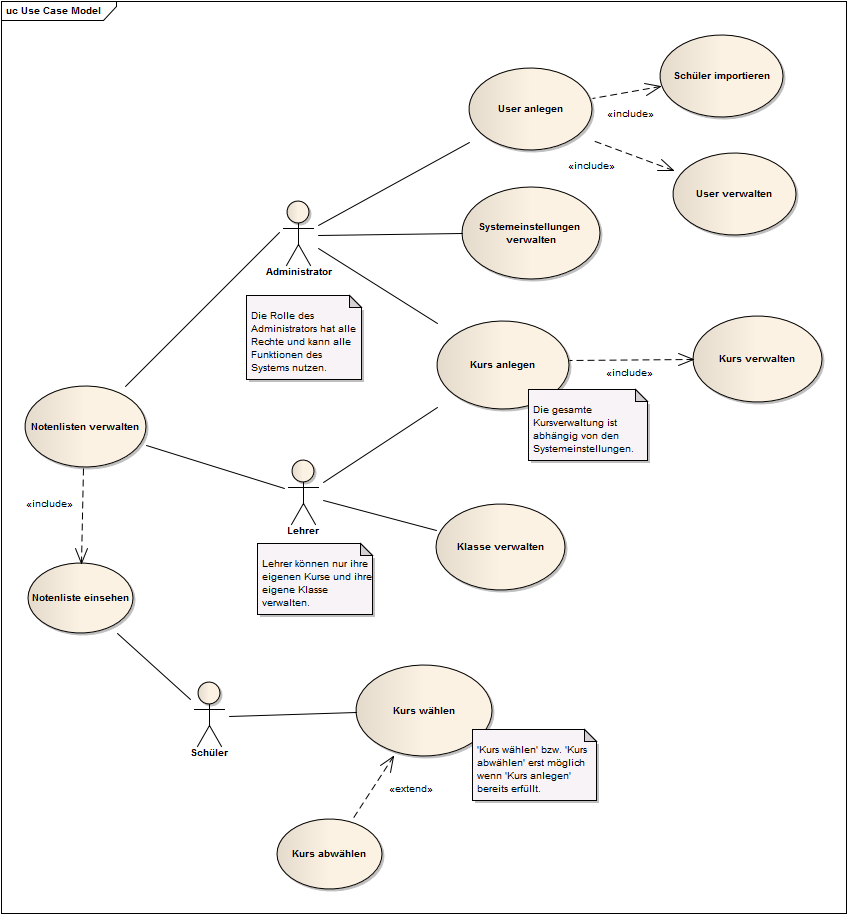
\includegraphics[scale=0.5]{img/UseCaseModel_kuwasys20.png}
 \end{center}
 \caption[\textbf{Use Case Diagram: Rollensystem}]{Use Case Diagramm: Rollensystem}
 \label{fig:UML_UC_kuwasys20}
\end{figure}

'Ein \ac{UC} beschreibt die Funktionalität des Softwaresystems, die ein Akteur ausführen muss, um ein gewünschtes Ergebnis zu erhalten oder um ein Ziel zu erreichen. \ac{UC}s sollen es ermöglichen, mit dem zukünftigen Benutzer über die Funktionalität des Softwaresystems zu sprechen, ohne sich gleich in Details zu verlieren.' Ein Zitat von \iz{Heide Balzert}{Informatikerin, die sich vor allem mit Fragen zum Thema Softwareengineering und -design beschäftigt. Derzeit ist sie Dozentin an der Fachhochschule Dortmund.}, entnommen aus \cite{BalzertH-UML2} auf Seite 28, welches den Sinn und Zweck eines \ac{UC-Diagramm}s präzise auf den Punkt bringt.

Zusammenfassend bedeutet dies, dass ein \ac{UC-Diagramm} immer dann sinnvoll ist wenn die Interaktionsmöglichkeit eines Systems, basierend auf verschiedene Aktueren, aufgezeigt werden soll. Die Akteure (dargestellt als 'Strichmännchen') im Diagramm, entsprechen genau denen, die später vom Rollensystem unterstützt werden sollen. Die Ellipsen zeigen die verschiedenen Anwendungsfälle die im System existieren. In einem so allgemeinen \ac{UC-Diagramm} wird absichtlich auf kleinste Details verzichtet. So bedeutet zum Beispiel der \ac{UC} 'Klasse verwalten' sowohl das Bearbeiten einer Klasse als auch das Vergeben von Noten oder andere klassenadministrative Aufwendungen.

Die gestrichelten Pfeile mit der Beschriftung '\texttt{$<<$include$>>$}' bezeichnen Anwendungsfälle in denen der \ac{UC}, auf welchen der Pfeil zeigt, implizit vorhanden ist wenn der \ac{UC}, von dem der Pfeil ausgeht, im System vorhanden ist. Das bedeutet wenn der \ac{UC} 'User anlegen' also vorhanden ist, auch die \ac{UC}s 'Schüler importieren' oder 'User verwalten' verwendet werden können. Ein erster \ac{UC} muss also immer erfolgen während ein zweiter (oder noch mehr) optional ausgeführt werden können.

Im Gegensatz hierzu bedeutet der gestrichelte Pfeil mit der Beschriftung '\texttt{$<<$extend$>>$}' von dem der Pfeil ausgeht, dass dieser \ac{UC} nur dann im System überhaupt vorhanden ist, wenn der \ac{UC} auf welchen der Pfeil zeigt im System vorhanden ist. Der \ac{UC} 'Kurs abwählen' ist also nur dann vorhanden wenn der \ac{UC} 'Kurs wählen' im System ausgeführt wurde. Der erste \ac{UC} wird durch den zweiten also erweitert.

\subsubsection{Statisches Analysemodell}

Im nächsten Schritt unserer Modellierung ist das statische Analysemodell, unter \prettyref{fig:UML_SA_kuwasys20} zu sehen, entworfen worden. Es stellt erste Überlegungen der Softwarearchitektur, mit konkreten Objekten inklusiver ihrer Attribute, dar und bildet ebenfalls die Beziehungen von Objekten zueinander ab. Genau genommen handelt es sich hierbei um ein 'abgespecktes' Klassendiagramm, in welchem die grobe Softwarestruktur erkennbar sein soll.

Die rechteckigen Formen stellen Klassen dar, die oben als Beschriftung ihren Namen tragen, unten die Attribute die zu ihr gehören. Die einfachen Linien sind Assoziationen zwischen den Klassen und können als Beziehungen interpretiert werden. Sie tragen einen Rollennamen und eine Multiplizität, um nachvollziehen zu können um wieviele Objekte einer Klasse es sich später mindestens und maximal handelt.
Die Rechtecke mit der Beschriftung \texttt{$<<$dataType$>>$ + String} stellen selbstdefinierte Datentypen dar.
Die Besonderheit in diesem Diagramm ist die Komposition (Assoziation mit einseitg schwarzer Raute). Sie sagt aus dass die Beziehung zwischen zwei Klassen einer starke Form der Aggregation entspricht. Die Teilklasse (Notenliste) kann also nur bestehen, solange die Aggregatklasse (Kurs) auch besteht. Würde, angewendet auf dieses Beispiel, ein Kurs gelöscht werden, würde auch der dazugehörige Notenlisteneintrag gelöscht werden. (Zur Vertiefung empfiehlt sich \cite{BalzertH_UML2} Seite 18)

In unserem Projekt entstanden zum Zeitpunkt des Softwareentwurfs 3 Klassen, die später für eine Interaktion mit dem System benötigt werden. Die Klasse für die Notenübersicht und für Kurse. Die verschiedenen Rollen wurden als Unterklassen der Klasse 'User' modelliert. Einzelne Datentypen, so bspw. für Daten zur Zeiterfassung (Datum) und zur Definition einzelner konstanter Strings (Name), wie die Rollen, wurden zur Vereinfachung vorgesehen.
Die Rollennamen sowie die Multiplizitäten der Assoziationen dürften selbsterklärend sein.

% Statisches Analyse Diagramm
\begin{figure}[H]
 \begin{center}
   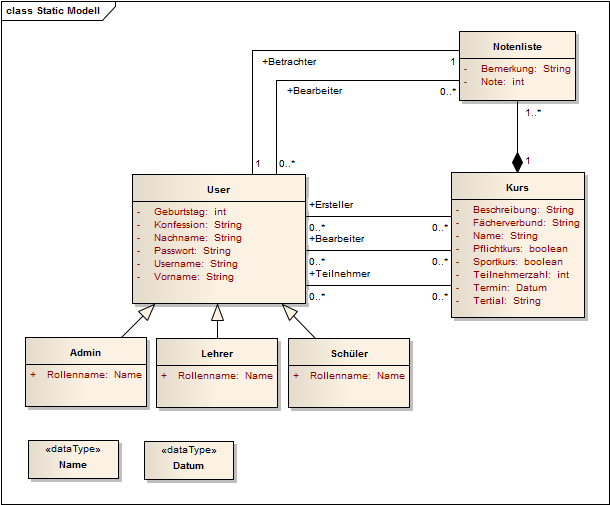
\includegraphics[scale=0.7]{img/StaticClassModel_kuwasys20.png}
 \end{center}
 \caption[\textbf{Statisches Analysemodell}]{Statisches Analysemodell}
 \label{fig:UML_SA_kuwasys20}
\end{figure}

\subsection{Benutzerschnittstellen und Rollensystem}\label{subsec:Benutzerschnittstellen und Rollensystem}

Das Kurswahlsystem der Schillerschule soll, laut Anforderungen, webbasiert mit Hilfe von verschiedenen Rollen konfiguriert und benutzt werden können.
Das System muss hierzu simultane Interaktionen, eines jeden Rollentyps, mit dem System zulassen. 

Per Aufgabendefinition liegen die vier Rollen, wie in \prettyref{subsec:Anforderungen an das System} bereits behandelt, zugrunde:

\begin{itemize}
  \item Schüler
  \item Kurslehrer
  \item Klassenlehrer
  \item Admin
\end{itemize}

Anhand der bereits vorgestellten \ac{OOM} sind, vor der Implementierung des Systems, die Rollenrechte und -richtlinien welche in den folgenden drei Unterabschnitten genaue beschrieben werden, modelliert worden.

\subsubsection{Die Rolle der Schüler}

Bei der Rolle der Schüler handelt es sich um die einfachste des Systems. 
Sie hat die wenigsten Rechte und kann hauptsächlich nur passiv, Ausnahme bildet hier die Kurswahl selbst, mit dem System interagieren.
Die Schüler welche das Kurswahlsystem erstmalig benutzen, befinden sich in der 7. Klasse. Jeder Schüler wird bis zum Abschluss der 9. Klasse das System benutzen.
Ein Schüler soll selbstständig seine Kurswahl für das jeweilige bevorstehende Tertial eines Schuljahres treffen können, dabei müssen bestimmte Abhängigkeiten eingehalten werden:

\begin{enumerate}
  \item 6 unterschiedliche Kurse pro Tertial
  \item 18 Kurse im Schuljahr
  \item 54 Kurse bis zur Vollendung des 9. Schuljahres
\end{enumerate}

\subsubsection{Die Rolle der Lehrer}

Der Rolle des Lehrers ist hingegen schon weitaus mehr Verantwortung auferlegt.
Das System unserer Webandwendung unterscheidet allerdings zwischen zwei verschiedenen Arten von Lehrern grundsätzlich nicht aufgrund einer Rollendefinition. 
Die Befugnis eines Lehrers sind lediglich abhängig von Werten die in der \ac{DB} gespeichert werden. 
Ein Klassenlehrer wird nur dann ein Klassenlehrer wenn für ihn eine Abhängigkeit zu einer Klasse besteht. 
Erst dann kann er die Funktionen, die einenm Klassenlehrer zu Verfügung stehen, nutzen.
Ein Klassenlehrer muss auf die ihm zugerordnete Klasse zugreifen und alle Kurse eines jeden Schülers einsehen können.

Das gleiche Prinzip gilt für Kurslehrer. 
Beim anlegen eines Kurses (eine Funktion die jedem Lehrer generell zur Verfügung steht) wird dieser Kurs dem Lehrer fest zugeordnet und wird somit zum Mitverantwortlichen der Kursverwaltung. 
Der Kurslehrer muss ebenfalls die Schüller einsehen können die sich in seinem Kurs befinden. Allerdings kann er nur ein Protokoll und eine Notenliste für Schüler in seinem Kurs führen.

In Abhängigkeit zur administrativen Systemverwaltung, auf die im nächsten Teil-Block eingegangen wird, hat der Lehrer nun die Rechte seine Kurse zu verwalten.

Zur Vereinfachung der Handhabung des Systems ist bereits an diesem Punkt der Modellierung an ein internes Protokollierungssystem gedacht worden. 
Es soll später die Kommunikation von Kurslehrern mit Klassenlehrern sowie die Kommunikation von Lehrern mit Schülern vereinfachen.
Im Rahmen unserer Projektarbeit wurde allerdings eine solche Funktionalität im System nicht implementiert.

\subsubsection{Die administrative Rolle des Systems}

Die administrativen Rechte des kompletten Systems stehen selbstverständlich nur dem Administrator zur Verfügung. Die Hauptaufgabe dieser Rolle im System ist es neue User ins System aufzunhemen und diese gegebenfalls zu Bearbeiten.
Das gilt für das Hinzufügen und Bearbeiten von Schülern und Lehrern gleichermaßen, beide Rollen haben also nicht die Möglichkeit sich selbst zu Verwalten.

Darüber hinaus verwaltet der Admin den Status des Systems, das aktuelle Schuljar und die dazughörigen Tertiale. Außerdem ist er der Hauptverantwortliche der Kursverwaltung.
Bevor ein Kurs stattfinden kann muss der Admin den Kurs aktivieren und für die Kurswahl zulassen. Eventuell müssen von ihm bestimmte Attribute eines Kurs noch angepasst werden können.
Ein Admin kann außerdem Fächerverbünde erstellen, bearbeiten und erstellte Kurse einem Fächerverbund zuordnen.

\subsubsection{Funktionalität des Systems}

Die Einteilung eines kompletten Schuljahrs geschieht jeweils in Tertiale. Dies kann grafisch in \prettyref{fig:Schuljahreinteilung} nachvollzogen werden. 

%%
% Schuljahreinteilung
\begin{figure}[h]
\begin{center}

\begin{tikzpicture}
    \node[draw=black, fill=yellow!20!] at (-2.5,5) {Unterteilung des Schuljahrs};
    \pie{33.3/Tertial 1, 33.3/Tertial 2, 33.3/Tertial 3}
\end{tikzpicture}

\end{center}
\caption[\textbf{Einteilung des Schuljahrs}]{Einteilung des Schuljahrs}
\label{fig:Schuljahreinteilung}
\end{figure}

Es war also nötig im administrativen Bereich des Systems eine Funktionalität vorzusehen, die es dem Admin ermöglicht das Schuljahr 'weiterzuschieben' und das entsprechende Tertial zu zu aktivieren.
Diese Verwaltungstätigkeit ist unumgänglich mit der Kurswahl verknüpft und muss für jede neu angepasst werden. 
Entscheidungen die hier während der Modellierung getroffen wurden, wurden im Hinblick auf eine möglichst einfaches \ac{UI} getroffen.

Jeder Kurs, der gewählt werden kann, gehört einem übergeordnetem Fächerverbund an, wie in \prettyref{fig:KursFaecherverbund} zu sehen ist.
Allerdings gibt es noch weitere Eigenschaften die Kurse erfüllen können. Ein Kurs kann ein Religionskurs sein, welcher für eine bestimmte Konfession ausgerichtet ist oder ein Sportkurs.
Ferner müssen Kurse als Pflichtkurse signifiziert werden können.
Aufgrund der Fülle an Informationen die verarbeitet werden müssen, war es in der Phase der Modellierung ebenfalls sehr wichtig die Datenstrukturen und deren Abhängigkeiten möglichst einfach zu halten, um in der späteren Implementierungsphase eine unkomplizierte Benutzerschnittstelle entwicklen zu können. 

%%
% Kurs - Fächerverbund
\begin{figure}[h]
\begin{center}

\begin{tikzpicture}
    \node[draw=black, fill=yellow!20!] at (-2.5,5) {Unterteilung des Schuljahrs};
    \pie{33.3/Tertial 1, 33.3/Tertial 2, 33.3/Tertial 3}
\end{tikzpicture}

\end{center}
\caption[\textbf{Einteilung des Schuljahrs}]{Einteilung des Schuljahrs}
\label{fig:KursFaecherverbund}
\end{figure}

%%
\todo[size=\small, color=green!40]{Grafik zur Abhängigkeit von Fächerverbünden bzw. Pflicht-/Sportkurse}
%%

Außer den beiden vorgestellten Datenverarbeitungen existieren selbstverständlich noch weitere, die vor allem im Sinne der Übersichtlichkeit des System  zum Tragen kommen. 
Dabei handelt es sich allerdings um Daten, die dynamisch während der Laufzeit erzeugt werden und deshalb ebenfalls in \prettyref{subsec:Systemrelevante Daten} genauer besprochen werden.
Im Gegensatz zu den dynamisch generierten Daten während der Laufzeit des Systems ist für alle anderen Daten zur Informationsverarbeitung eine Speicherung in einer Datenbank unabdingbar.
Im folgenden Unterabschnitt soll deshalb näher auf die Modellierung und Umsetzung des verwendeten Informationssystems eingegangen werden.

\subsection{Datenbankmodellierung}\label{subsec:Datenbankmodellierung}

Für die \ac{DB}-Modellierung wurde als erstes ein \ac{ER-Modell} skizziert, welches die Abhängigkeiten und Beziehungen zueinander verdeutlichen soll. Dieses ist in \prettyref{subsec:ERModell} abgebildet. Anschließend wurde das gesamte \ac{ER-Modell} in ein relationales Modell transformiert.
Mit dem entstandenen Relationalen Modell, welche in \prettyref{subsec:RelModell} dokumentiert ist, konnte anschließend auf dem Server die \ac{DB} inklusive der nötigen Tabellen erstellt werden.

\subsubsection{Entity-Relationship Modell}\label{subsec:ERModell}

Die \prettyref{fig:ERModell} zeigt das oben erwähnte \ac{ER-Modell} nach \iz{Peter Pin-Shan Chen}{Informatiker, der 1976 das ER-Modell entwickelte. Er gilt heute als Pioneer der \ac{OOM}.}, nachzulesen unter \cite{ChenPe} Seite 3 ff. bzw. \cite{VossenG-DDD} ab Seite 60.

\textbf{Aufbau des \ac{ER-Modell}s:}

Bei den blauen Rechtecken handelt es sich in diesem Modell um sogenannte Entities (Entity-Typen), die sind Dinge die in der \ac{DB} als solche abgebildet werden sollen. Sie stellen eine eigene Tabelle dar. Die gelben Ellipsen die diese umgeben, sind die Attribute (Attribut-Typen) der Entities, sie veranschaulichen die Daten welche Entities enthalten (können).
Die roten Rauten bezeichnen Beziehungen (Beziehungs-Typen) die zwischen Entities herrschen.

Das grüne Rechteck ist ein Spezialfall des 'Kurs'-Entities. Es wird als eigene Tabelle in der \ac{DB} dargestellt, ist im weitesten Sinne allerdings einer Aversion des 'Konfessions'-Attribut des 'Kurs'-Entities. Denkt man in diesem Fall an die \ac{UML}, so wäre an dieser Stelle wohl eine 'Enumeration' als eigener Datentype in Frage gekommen (Vrgl. \cite{BalzertH_UML2} Seite 10 und 11).

\tikzstyle{every entity} = [top color=white, bottom color=blue!30, draw=blue!50!black!100, drop shadow]
\tikzstyle{every weak entity} = [drop shadow={shadow xshift=.7ex, shadow yshift=-.7ex}]
\tikzstyle{every attribute} = [top color=white, bottom color=yellow!20, draw=yellow, node distance=1cm, drop shadow]
\tikzstyle{every relationship} = [top color=white, bottom color=red!20, draw=red!50!black!100, drop shadow]
\tikzstyle{every isa} = [top color=white, bottom color=green!20, draw=green!50!black!100, drop shadow]
\begin{center}
\begin{figure}[H]

\scalebox{.7}{
\begin{tikzpicture}[node distance=1.5cm, every edge/.style={link}]

%% USER
\node[entity] (usr) {Users};
\node[attribute] (usrvname) [above=2.5cm of usr] {VName} edge (usr);
\node[attribute] (usrnname) [above right=3cm of usr] {NName} edge (usr);
\node[attribute] (geb) [above left=3cm of usr] {Geburtsdatum} edge (usr);
\node[attribute] (usrkonf) [above left=of usr] {Konfession} edge (usr);
\node[attribute] (usrklasse) [above=of usr] {Klasse} edge (usr);
\node[attribute] (usrusername) [above right=of usr] {\key{Username}} edge (usr);
\node[attribute] (usrpassword) [right=of usr] {Passwort} edge (usr);
\node[attribute] (usrid) [below=0.3cm of usr] {\key{UserID}} edge (usr);

%% REL "hat"
\node[relationship] (hat) [left=1.5cm of usr] {hat} edge (usr);

%% REL "eingetragen"
\node[relationship] (eingetragen) [below left =3cm of usr] {eingetragen} edge (usr);
%
%% ROLLE
\node[entity] (rolle) [left=1cm of hat] {Rolle} edge (hat);
\node[attribute] (rollename) [left=of rolle] {\key{Username}} edge (rolle);
\node[attribute] (rolleusrnname) [above left=of rolle] {Rolle} edge (rolle);

%% REL "besucht"
\node[relationship] (besucht) [below right=of usr] {besucht} edge (usr);

%% KURS
\node[entity] (kurs) [below right=1cm of besucht] {Kurs} edge (besucht);
\node[entity, top color=white, bottom color=green!30, draw=green!50!black!100, drop shadow] (kurskonf) [above=1.5cm of kurs] {Kurskonfession} edge (kurs);
\node[attribute] (termin) [above right =.2cm of kurskonf] {Termin} edge (kurs);
\node[attribute] (kursl) [right =.2cm of kurskonf] {Kurslehrer} edge (kurs);
\node[attribute] (teilm) [above right=0.2cm of kurs] {Teilnehmerzahl} edge (kurs);
\node[attribute] (kursid) [left=0.2cm of kurs] {\key{KursID}} edge (kurs);
\node[attribute] (faecher) [right=0.2cm of kurs] {Fächerverbund} edge (kurs);
\node[attribute] (flags) [below=2.5cm of kurs] {Sportkurs} edge (kurs);
\node[attribute] (flag3) [below=2.2cm of faecher] {Pflicht} edge (kurs);
\node[attribute] (tertial) [below left=.2cm of flag3] {Tertial} edge (kurs);
\node[attribute] (flag2) [below=1.2cm of faecher] {Konfession} edge (kurs);
\node[attribute] (bemerk) [below=of kurs] {Beschreibung} edge (kurs);
\node[attribute] (kursname) [below right=0.2cm of kurs] {Kursname} edge (kurs);

%% REL "enthält"
\node[relationship] (enthalten) [below left =of kurs] {enthalten} edge (kurs);

%% NOTENLISTE
\node[entity] (notenliste) [below right=2cm of eingetragen] {Notenliste} edge (enthalten) edge (eingetragen);
\node[attribute] (note) [below left=1cm of notenliste] {Note} edge (notenliste);
\node[attribute] (usrkonf) [above =of notenliste] {Bemerkung} edge (notenliste);
\node[attribute] (usrvname) [below=of notenliste] {\key{KursID}} edge (notenliste);
\node[attribute] (usrnname) [left=of notenliste] {\key{UserID}} edge (notenliste);
\node[attribute] (listid) [below right=1.2cm of notenliste] {\key{ListenID}} edge (notenliste);

%% SYSTEM
\node[entity] (system) [below=5cm of notenliste] {System};
\node[attribute] (schuljahr) [below=of system] {Schuljahr} edge (system);
\node[attribute] (tertial) [left=of system] {Tertial} edge (system);
\node[attribute] (wochd) [below left= of system] {Phase} edge (system);
\end{tikzpicture}
}
\caption[\textbf{Entity-Relationship Modell}]{Entity-Relationship Modell}
\label{fig:ERModell}
\end{figure}
\end{center}

\textbf{Interpretation des \ac{ER-Modell}s:}

Um die Interpretation, also den Gedankengang der \ac{DB}-Modellierung, zu verdeutlichen macht es Sinn, die Beziehungen genau auszuformulieren.
Dabei werden alle Beziehungen zu jedem Entity betrachtet, begonnen mit dem Entity.
Zusätzlich sollen die Multiplizitäten mit einfließen, um die Abhängigkeiten zu verdeutlichen und um die Transformation in ein Datenbankmodell zu erleichtern.

Die Schreibweise dieser Multiplizitäten ist wie folgt definiert:

Sei $E_{A}$ das erste und $E_{B}$ das zweite Entity.
Die Beziehung beider Entities ist definiert als $R_{AB}$. 
Die erste Multipliziät $(0,N)$ gibt Auskunft über die Häufigkeit von $E_{A}$ in der geltenden Beziehung zu $E_{B}$.
Die zweite $(1;M)$ über die Häufigkeit von $E_{B}$ zu $E_{A}$.

Man kann also schreiben:

\begin{center}
$E_{A}$ ist $(0;N)$ in Beziehung $R_{AB}$ zu $E_{B}$

oder

$E_{B}$ ist $(1;M)$ in Beziehung $R_{AB}$ zu $E_{A}$
\end{center}

Wobei die erste Zahl bei der Angabe der Multiplizität, also die vor dem Semikolon (';') für die minimalste, die zweite Zahl für die maximalste Gültigkeit unter der bestendenen Bedingung steht.

Begonnen werden soll die genauere Betrachtungsweise mit dem Entity 'User':

\begin{enumerate}
  \item User - Rolle (beidseitig):	
    \begin{itemize}
      \item einem User ist genau $(1;1)$ Rolle zugeteilt
      \item einer Rolle hingegen können $(0;N)$ User zugeteilt sein
    \end{itemize}

  \item User - Kurs
    \begin{itemize}
      \item ein Schüler wählt $(0;N)$ viele Kurse
      \item ein Lehrer erstellt/verwaltet $(0;M)$ viele Kurse
    \end{itemize}
  
  \item User - Notenliste:
    \begin{itemize}
      \item ein Schüler hat $(1;1)$ Eintrag in der Notenliste für jeweils einen fest zugeordneten Kurs (Vrgl. Kurs - Notenliste)
    \end{itemize}

\end{enumerate}

Konkretisieren wir nun das Entity 'Kurs':

\begin{enumerate}
  \item Kurs - Notenliste:
  \begin{itemize}
    \item ein Kurs besitzt genau $(1;1)$ Eintrag pro Kurs in der Notenliste für einen Schüler (Vrgl. User - Notenliste)
  \end{itemize}
  
  \item Kurs - Kurskonfession	
    \begin{itemize}
      \item ein Kurs hat genau $(0;1)$ Konfessionszugehörigkeit
    \end{itemize}

  \item Kurs - User	
    \begin{itemize}
      \item ein Kurs wird von $(0;N)$ vielen Schülern gewählt
      \item ein Kurs wird immer genau $(1;1)$ Lehrern zugeteilt
    \end{itemize}
\end{enumerate}

Für das letzte Entity der Dreier-Beziehung 'Notenliste' gelten lediglich die bereits beschriebenen Abhängigkeiten und Beziehungsverhältnisse. 
Zur Verdeutlichung sollen diese jedoch nochmals aufgeführt werden.

\begin{enumerate}
  \item Notenliste - User:
  \begin{itemize}
    \item eine Notenliste hat im Bezug auf genau einen Kurs $(0;N)$ Einträge für einen User
  \end{itemize}
  
  \item Notenliste - Kurs:
  \begin{itemize}
    \item Ein Schüler wählt $(1;N)$ viele Kurse, ein Kurs wird von $(1;N)$ vielen Schülern besucht/gewählt.
  \end{itemize}
  
\end{enumerate}

Das Entity 'System' besitzt keine Beziehungen innerhalb der Datenbank, weshalb auf eine ausführliche Interpretation verzichtet werden kann.
Die Darstellung dieses Entities wird innerhalb der \ac{DB} sowieso über eine eigene Tabelle umgesetzt.

Der nächste Schritt ist nun die Transformation von \ac{ER-Modell} in das Relationale \ac{DB}-Modell.

\subsubsection{Relationales Modell}\label{subsec:RelModell}

Bei der Beschreibung des Relationalen Modells der KuWaSys-\ac{DB} ist das Hauptaugenmerk auf die komplette Datenverarbeitung gelegt, also vor allem auch Implementierungen für Vorgänge die für den Benutzer des Systems nicht unmittelbar zu sehen sind.
Daten die für die Oberfläche und die einzelnen Benutzerschnittstellen eine tragende Rolle spielen sollen unter (Abschnitt Benutzerschnittstellen) gesondert behandelt werden und werden im Laufe dieses Kapitels nur kurz angesprochen.

Die Vorüberlegungen zur Transformation von mehrwertigen Attributen von Entities sind bereits abgeschlossen.
Prinzipiell kann man mit der Transformation, wie in \cite{VossenG-DDD} beschrieben ist wie folgt vorgehen:

\begin{enumerate}
 \item Jedes Entity wird in eine relationale Form gebracht
 \item Jeder Beziehungs-Typ ebenfalls, es sei denn:
 \begin{itemize}
  \item es handelt sich um eine zweistellige $1:1$-Beziehung
  \item es handelt sich hierbei um eine $1:N$-Beziehung
 \end{itemize}
\end{enumerate}

Die Beschreibung $1:1$- bzw $1:N$-Beziehung bedeutet in diesem Fall allerdings nicht wie zuvor, ein Minimum auf der linken und das Maximum auf der rechten Seite. 
Hierbei werden nur noch die maximalen Werte der beiden Multiplizitätsangaben berücksichtigt. Dies gilt analog für alle Angaben der Multiplizitäten.

Sollte bei der Transformation $Punkt$ $2)$ eine Rolle spielen, müssen Attribute in bereits bestehende Relationsschemata aufgenommen werden. Folgende Regeln treten dann in Kraft:
\begin{enumerate}
 \item Zweistellige $1:1$-Beziehung
 \begin{itemize}
  \item ein Entity stellt selbst ein Relationsschema dar
  \item Attribute des zweiten Entities werden ebenfalls in dieselbe Tabelle gespeichert
 \end{itemize}
 \item Zweistellige $1:N$-Beziehung
 \begin{itemize}
  \item ein Entity stellt ein eigenes Relationsschema dar
  \item erste Möglichkeit: die Attribute des Entities welches die maximale Multiplizität von $1$ aufweist wird hingegen dem Realtionsschema mit der maximalen Multiplizität von $N$ in Form von Fremdschlüsseln zugeschrieben
  \item zweite Möglichkeit: es wird ein eigenes Relationsschema für die Beziehung der beiden Entities angelegt. Dieses neu entstande Schema erhält dann Attribute, welche widerum Fremdschlüssel der beiden anderen Entities sind
 \end{itemize}
\end{enumerate}

Die Transformation vom \ac{ER-Modell} ins Relationale Modell (zur bildhaften Darstellung ist die Kopfzeile der dazugehörigen Tabelle auch gezeigt) sieht im Falle des Kurswahlsystems folgendermaßen aus:

\textbf{Users} = \{( \underline{id:serial}, nachname:character, vorname:character, geburtstag:character, konfession:character, klasse:character, \underline{username:character}, passwort:character )\}

% User-Tabelle
\begin{table}[H]
\begin{center}
	\begin{tabular}{|c|c|c|c|c|c|c|c|}\hline
		\textbf{\underline{ID}} & \textbf{NName} & \textbf{VName} & \textbf{Geb} & \textbf{Konf} & \textbf{Klasse} & \textbf{\underline{Username}} & \textbf{Passwort} \\ \hline
		\vdots & \vdots & \vdots & \vdots & \vdots & \vdots & \vdots & \vdots \\
	\end{tabular}
	\caption{Kopfzeile der User-Tabelle}
\end{center}
\end{table}

\textbf{Kurs} = \{( \underline{id:serial}, name:character, kurslehrer:integer, faecherverbund:character, termin:integer, beschreibung:character, schuljahr:integer, tertial:integer, 
teilnehmerzahl:integer, pflichtkurs:boolean, sport:boolean )\}

% Kurs-Tabelle
\begin{table}[H]
\begin{center}
	\begin{tabular}{|c|c|c|c|c|c}\hline
		\textbf{\underline{ID}} & \textbf{Name} & \textbf{Kurslehrer} & \textbf{Faecherverbund} & \textbf{Termin} & \dots \\ \hline
		\vdots & \vdots & \vdots & \vdots & \vdots & \dots \\
	\end{tabular}
	\caption{Kopfzeile der Kurs-Tabelle  (unvollständig)}
\end{center}
\end{table}

\textbf{Kurs-Konfessionen} = \{( \underline{religionid:integer}, konfession:character )\} 
 
% Kurs-Konfession-Tabelle
\begin{table}[H]
\begin{center}
	\begin{tabular}{|c|c|}\hline
		\textbf{\underline{ReligionID}} & \textbf{Konfession} \\ \hline
		\vdots & \vdots \\
	\end{tabular}
	\caption{Kopfzeile der Kurs-Konfessions-Tabelle}
\end{center}
\end{table}

\textbf{Notenliste} = \{( \underline{id:serial}, note:integer, bemerkung:character, userid:integer, kursid:integer, jahr:integer, tertial:integer )\}

% Notenliste-Tabelle
\begin{table}[H]
\begin{center}
	\begin{tabular}{|c|c|c|c|c|c|c|}\hline
		\textbf{\underline{ID}} & \textbf{Note} & \textbf{Bemerkung} & \textbf{UserID} & \textbf{KursID} & \textbf{Jahr} & \textbf{Tertial}\\ \hline
		\vdots & \vdots & \vdots & \vdots & \vdots & \vdots & \vdots  \\
	\end{tabular}
	\caption{Kopfzeile der Notenlisten-Tabelle}
\end{center}
\end{table}

\textbf{Rolle} = \{( \underline{username:character}, rolle:character )\}

% Rollen-Tabelle
\begin{table}[H]
\begin{center}
	\begin{tabular}{|c|c|}\hline
		\textbf{\underline{Username}} & \textbf{Rolle} \\ \hline
		\vdots & \vdots \\
	\end{tabular}
	\caption{Kopfzeile der Rollen-Tabelle}
\end{center}
\end{table}

\textbf{System} = \{( \underline{phase:integer}, jahr:integer, tertial:integer )\}

% System-Tabelle
\begin{table}[H]
\begin{center}
	\begin{tabular}{|c|c|c|}\hline
		\textbf{\underline{Phase}} & \textbf{Jahr} & \textbf{Tertial} \\ \hline
		\vdots & \vdots & \vdots \\
	\end{tabular}
	\caption{Kopfzeile der System-Tabelle}
\end{center}
\end{table}

\subsection{Konfiguration der Laufzeitumgebung und des Servers}\label{subsec:Konfiguration der Laufzeitumgebung und des Server}

Dieses Kapitel ist als Zwischenschritt, von der Modellierung zur Implementierung, unseres Softwareprojekts zu verstehen.
Zum Einen galt es eine komplette bestehende Infrastruktur zu überblicken und zu verstehen (dieser Schritt kann als eine Art der Modellierung verstanden werden)
zum Anderen musste ein komplettes neues System einwandfrei funktionsfähig eingebettet werden (zu vergleichen mit dem Schritt der Implementierung).

\textbf{Sichtung der bestehenden Infrastruktur:}

Die Schillerschule teilt sich mit der benachbarten Realschule am Galgenberg eine Serverinfrastruktur nach der Novell Musterlösung paedML 3.33, weitere Informationen sind unter \cite{paedML} zu finden. % VMWare ASG 220 Astaro.
Diese beinhaltet eine virtuelle Infrastruktur \gls{VMWare} ESXi auf der ein \ac{SLES} Novell Server gehostet ist.

\begin{figure}[H]
\begin{center}
\begin{tikzpicture}[
  scale=0.1,
  font=\sffamily,
  every matrix/.style={ampersand replacement=\&,column sep=2cm,row sep=2cm},
  source/.style={draw,thick,rounded corners,fill=yellow!20,inner sep=.3cm},
  process/.style={draw,thick,circle,fill=blue!20},
  sink/.style={source,fill=green!20},
  datastore/.style={draw,very thick,shape=datastore,inner sep=.3cm},
  dots/.style={gray,scale=2},
  to/.style={->,>=stealth',shorten >=1pt,semithick,font=\sffamily\footnotesize},
  every node/.style={align=center}]

  % Positionierung über Matrix-Layout
  \matrix{

    \node[source] (Ubuntu) {Ubuntu 12.04 VM\\ ($141.10.50.250$)};
      \& \node[process] (Suse) {Server}; \& \\
      \& \node[sink] (firewall) {ASG 220 Astaro\\ ($Firewall$)}; \& \\

    \node[source] (SLES) {SuSE Linux\\ Enterprise Server\\ ($SLES$)}; \& \\

    \node[datastore, color=black!50!white] (infrastructure) {Einstellungen\\($Novell$ $paedML$ $3.3$)}; \& \\


      \& \node[process] (router) {Router};
      \& \node[sink] (www) {WWW}; \\
  };

  % VM - Host
  \draw[to, very thick] (Ubuntu) -- node[midway,above] {VM Host}
      node[midway,below] {} (Suse);

  % FW - Host
  \draw[to, dashed, very  thick] (Suse) -- node[midway,above] {}
       node[midway,below] {} (firewall);itemize
  \draw[to, dashed, very  thick] (firewall) -- node[midway,above] {}
       node[midway,below] {} (Suse);

  % FW - Router
  \draw[to, very thick] (router) -- node[midway,above] {}
       node[midway,below] {} (firewall);
  \draw[to, very  thick] (firewall) -- node[midway,above] {}
       node[midway,below] {} (router);

  % Einstellungen Infrastruktur
  \draw[color=black!50!white] (infrastructure) -- node[midway,above] {}
       node[midway,below] {} (SLES);

  % SLES - Netz
  \draw[to, very thick] (SLES) -- node[midway,above=1cm] {VM Host}
       node[midway,below] {} (Suse);
  \draw[to, dashed, color=black!50!white] (SLES) -- node[midway,right=0.2cm] {Konfiguration}
       node[midway,below] {} (router);
  \draw[to, dashed, color=black!50!white] (SLES) -- node[midway,right=0.2cm] {Konfiguation}
       node[midway,below] {} (Ubuntu);

  % Router - WWW
  \draw[to, very thick] (router) -- node[midway,above] {}
       node[midway,below] {} (www);
  \draw[to, very thick] (www) -- node[midway,above] {}
       node[midway,below] {} (router);
\end{tikzpicture}
\end{center}
\caption[\textbf{Netzwerkstruktur der Schillerschule Aalen}]{Netzwerkstruktur der Schillerschule Aalen mit DMZ}
\label{fig:Netzwerkstruktur}
\end{figure}

Prinzipiell wäre eine Verwendung dieser virtuellen \gls{Appliance} zum Hosting der \ac{Webapp} möglich. Um jedoch die Systemsicherheit zu erhöhen ist eine weitere virtuelle Appliance, die nur das Kurswahlsystem bereitstellt die bessere Wahl.
\iz{Ubuntu Server 12.04 LTS}{http://www.ubuntu.com/} läuft auf diesem virtuellen Rechner, der sich wie der oben genannte SLES in der \gls{DMZ} der virtuellen Netzwerkinfrastruktur befindet.

\textbf{Integration in die Infrastruktur:}

Ein PostreSQL-Server dient zur Datenhaltung und ein Apache Tomcat 7 zur Auslieferung der \ac{Webapp}. Nach Konfiguation (und überfälligem reboot) der Astaro Firewall im Keller der Schule ist die Webapp jetzt über das Intranet an allen Rechnern im Schulnetz erreichbar (\url{http://192.168.1.222:8080/kuwasys20}). Die Erreichbarkeit über das Internet ist seit der Freischaltung der entsprechenden Ports auf den BelWü-Server und umgekehrt gegeben (\url{http://141.10.50.250:8080/kuwasys20}).
Diese Adressen werden auf der Homepage der Schillerschule und im Intranet verlinkt, sodass keine weitere Maskierung wie Subdomains oder lokale DNS-Einträge notwendig ist.
Die Admnistration des Ubuntu Servers kann im Intranet von einer VMWare Management Console aus erfolgen, für schnelles Eingreifen wurde ein \gls{Secure Shell} (SSH) Zugang eingerichtet, der im Internet erreichbar ist.

In \prettyref{fig:Netzwerkstruktur} ist die neue Struktur des Netzwerks dargestellt.

Die Einrichtung eines Backups war für unser Projekt nicht notwendig, da die Schillerschule selbst schon über ein funktionsfähiges Backupsystem verfügt. Hierbei wird in bestimmten Intervallen die komplette Festplatte des Servers gespiegelt, und somit auch die virtuellen Maschinen.
Somit ist die Garantie gegeben, dass auch das Kurswahlsystem einem ständigen Sicherungsvorgang unterliegt und im Notfall wiederhergestellt werden kann.
\newpage

\section{Implementierung}	\label{sec:Implementierung}
							\label{secmin:Implementierung}

In einem System, in welchem ein \gls{Multi-User Betrieb} möglich sein soll, ist das Design der Oberfläche und das der einzelnen Benutzerschnittstellen unweigerlich eng miteinander verknüpft. 
Es müssen in der Phase der Implementierung bereits exakte Schnittstellen definiert und strukturierte Oberflächen skizziert worden sein um spätere Korrekturen gering zu halten oder um sie zu vermeiden.

In den folgenden zwei Abschnitten sollen grundlegende Implementierungsgedanken besprochen werden, die mit den Anforderungen an das System in erster Linie nichts zu tun haben. 
Zuerst soll die Art und Weise der Umsetzung der Benutzerschnittstellen und des Designs näher erklärt werden. Danach sollen elementare Datenstrukturen die zum Einsatz kamen und in JSF implementiert wurde näher erläutert werden.

Nach den beiden einführenden Abschnitten wird dem Leser detailiert dargestellt wie die zu bewältigenden Systemanforderungen in JSF umgesetzt wurden. 
Dabei werden Quellcodeausschnitte sowie Diagramme zum Einsatz kommen die dem Leser das Verstehen erleichtern sollen.
Da während allen Phasen der Umsetzung des Projekts auch immer die Modularität des gesamten Systems im Vordergrund stand soll hier nicht kleinlichst genau erklärt werden was im Quellcode steht, sondern darauf eingegangen werden, wie das zu lösende Problem angegangen wurde und schlussendlich welche wichtigen Bausteine zu tragen kamen. 
An dieser Stelle soll außerdem nochmals die Wichtigkeit der oben besprochenen Datenbankmodellierung erwähnt werden. Gründe für die verschiedenen Umsetzungen der Modellierung sollen im Abschnitt der Implementierung dieser Ausarbeitung nicht mehr näher besprochen werden. 
Es wurde jedoch viel Wert darauf gelegt die Schritte der Implementierung gut und verständlich zu formulieren und darzustellen.

\subsection{Benutzerschnittstellen und Oberflächendesign}

Wir haben uns für ein simples und einfach zu verstehendes Oberflächendesign entschieden, welches allerdings den Design Aspekten der \gls{Corporate Identity} (CI) erfüllen sollte. 
%%
\todo[size=\small, color=green!40]{HMI Buch Zitate etc...}
%%
Im allgemeinen wird beim Screendesign bestimmten Regeln gefolgt, welche durch das gewählte Gestaltungsraster festgelegt werden.

Hierzu wurden von uns folgende Bereiche festgelegt:
\begin{itemize}
  \item Kopf- oder Bannerbereich mit Logo
  \item Navigationsbereich bzw. Unternavigation
  \item Arbeitsbereich
  \item Impressum/Hinweise
\end{itemize}

Der Hauptaufbau dieser Seiten, auf welche im folgenden näher eingegangen wird, wurden mit Templates, wie es bereits in \prettyref{subsec:Darstellung von Seiteninhalten} angesprochen wurde, umgesetzt.
Der allgemeine Aufbau soll im folgenden besprochen werden, der nachstehende Quellcodeausschnitt zeigt einen Teil des Templates das von uns zur Gestaltung der Seiten verwendet wurde:

% LISTING
% template.xhtml 
%%
\todo[size=\small, color=red!40]{Listing}
%%
Auffallend ist vor allem der Kopf der Seite, welcher den Wiedererkennungswert (Vrgl. hierzu die \iz{Webiste der Schillerschule}{\url{http://www.schillerschule-aalen.de}}) ganu im Sinne des \ac{CI}s steigern soll.
Hierzu wurde die Grafik lediglich transparenter gehalten als ihr Original und hat ganz im Stil der Schule die Überschrift erhalten wie in \prettyref{fig:header_KuWaSys} zu sehen ist.

% Header
\begin{figure}[H]
 \begin{center}
   
\includegraphics[scale=0.4]{img/header_KuWaSys.png}
 \end{center}
 \caption[\textbf{KuWaSys: Banner des Systems (Header)}]{KuWaSys: Banner des Systems (Header)}
 \label{fig:header_KuWaSys}
\end{figure}

Die Navigation und deren Unternavigationspunkte sind im linken Bereich der Webiste angeordnet und unterstützen den User visuell mit Hervorhebungen, wie in \prettyref{fig:navihervorhebung_KuWaSys} dargestellt ist, bei der Arbeit mit dem System.
Nötige Unternavigationspunkte, falls diese vorhanden sind, öffnen sich automatisch beim Klick auf ein übergeordnetes Menüelement, sodass die komplette Menüstruktur handlich und kompakt dargestellt erscheint und mit einem Blick erfasst werden kann.

Der Arbeitsbereich wird in der Mitte der Seite dargestellt, unterhalb des Kopfbereichs und rechts der Navigation. 
Dieser wird abgetrennt durch blaue Balken (links zur Navigation sowie oben zum Kopfbereich) um die Einteilung der Seite für die Benutzer des Systems eindeutig und übersichtlich zu halten.
Jede Interaktion mit dem System wird in diesem Bereich der Website dargestellt. 
%%
\todo[size=\small, color=green!40]{Grafik zu Bildschirmenteilung}
%%

% Infobar
\begin{figure}[h]
 \begin{center}
   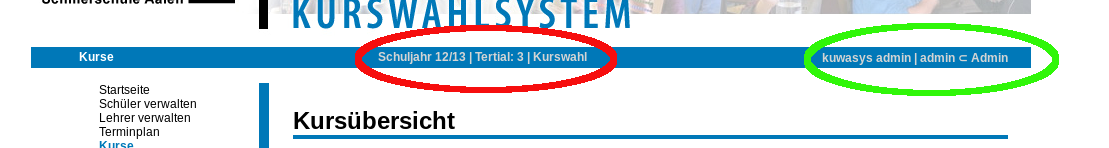
\includegraphics[scale=0.4]{img/informationbar_KuWaSys.png}
 \end{center}
 \caption[\textbf{KuWaSys: Informationsbalken (oberer Bereich)}]{KuWaSys: Informationsbalken (oberer Bereich)}
 \label{fig:infobar_KuWaSys}
\end{figure}

Zur erwähnen ist zudem noch der Trennbalken nach oben welcher zusätzlich als Informationsanzeige für den User verwendet wird und der Fußbereich welcher Informationen zur Website enthält. 
Die obere Anzeige, hier werden Informationen zum User selbst (Voller Name, Username und Rolle im System) und Informationen zum aktuellen Status des Systems (aktuelles Schuljahr und aktuelles Tertial) angezeigt.
Die \prettyref{fig:infobar_KuWaSys} zeigt die genaue Einteilung des Infobalkens oben, rot die Informationen des Systems, grün die Informationen des Users.
Der Fußbereich dient ausschließlich zur weiteren Information beim Besuch der Webiste welcher in \prettyref{fig:footer_KuWaSys} zu sehen ist.  

Die Hauptfarben des Systems wurden absichtlich blau gewählt um eine gewisse Professionalität sowie Seriösität gegenüber den Benutzern auszustrahlen. Diese ziehen sich kontinuierlich durch das gesamte System

%%
\todo[size=\small, color=green!40]{HMI Buch Dahm...}
%%

% Navibar
\begin{wrapfigure}[18]{r}{12cm}
 \begin{center}
   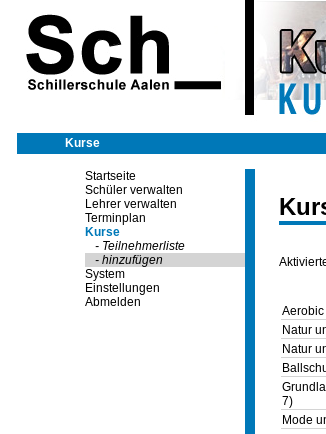
\includegraphics[scale=0.65]{img/navigation_KuWaSys.png}
 \end{center}
 \caption[\textbf{KuWaSys: Navigations und Menüelemente (linker Bereich)}]{KuWaSys: Navigations und Menüelemente (linker Bereich)}
 \label{fig:navihervorhebung_KuWaSys}
\end{wrapfigure}

Auf ein Impressum oder auf rechtliche Hinweise konnte bei dieser Art von Webiste verzichtet werden. 
Erstens handelt es sich hierbei um keine kommerzielle Website, laut \textit{§5} \ac{TMG} wird ein Impressum von 'geschäftsmäßigen Online-Diensten' benötigt, 
%%
\todo[size=\small, color=green!40]{rechtlicher Nachweis} zweitens um keine öffentliche oder frei zugängliche Website, 
%%
wobei hier die Vorschrift des \textit{§55} \ac{RstV} besagt, dass eine Impressumspflicht nur dann besteht wenn der Inhalt der Website regelmäßig journalistisch-redaktionelle Inhalte online zur Verfügung stellt.
(Gesetzesauszüge sind im Anhang unter \prettyref{subsec:Gesetz} zu finden) 

% Footer
\begin{figure}[h]
 \begin{center}
   
\includegraphics[scale=0.7]{img/footer_KuWaSys.png}
 \end{center}
 \caption[\textbf{KuWaSys: Informationsbalken (unterer Bereich)}]{KuWaSys: Informationsbalken (unterer Bereich)}
 \label{fig:footer_KuWaSys}
\end{figure}

Zur Strukturierung von Seiteninhalten wurden herkömmliche \ac{JSF}-Standardkomponenten verwendet.
Zu den hauptsächlich verwendeten, zählen:
\begin{itemize}
  \item \texttt{<h:outputText>}\\
    Element welches HTML-Text auf der Obefläche ausgibt 
  
  \item \texttt{<h:outputLabel>}\\
    auch normaler Text, allerdings als Beschriftung von Texteingabefeldern
      
  \item \texttt{<h:inputText>}\\
    Element zur Texteingabe, Synonyme für ein HTML \texttt{<input>}-Tag mit type="text"
  
  \item \texttt{<h:inputSecret>}\\
    Element zur verschlüsselten Texteingabe, entspricht \texttt{<input>}-Tag mit type="password"
  
  \item \texttt{<h:commandButton>}\\
    Button in HTML, der Klick löst eine definierte Aktion über eine ManagedBean-Methode aus

  \item \texttt{<h:panelGrid>}\\
    Darstellung einer Tabelle, Synonym für das HTML \texttt{<table>}-Tag. Die Anzahl der Spalten wird über das \texttt{columns}-Attribut festgelegt
  
  \item \texttt{<h:panelGroup>}\\
    Container-Element (mehrere JSF-Tags werden zu einem zusammenfügt)
  
  \item \texttt{<h:message>}\\
    gibt eine Fehlermeldung für die definierte Komponenten aus (\texttt{ErrorStyle}-Attribut über \ac{CSS} steuerbar)
  
  \item \texttt{<h:form>}\\
    stellt ein Formular dar, welches einen POST-Request per HTTP absetzt
  
  \item \texttt{<f:facet>}\\
    Definiert eine Facette (bspw. die Überschrift für eine Tabelle)
\end{itemize}

Außer den eben erwähnten Komponenten gibt es eine Vielzahl anderer bis hin zu selbstdefinierten welche im entwickelten System zum Einsatz kommen. Diese werden allerdings nicht näher betrachtet, da sie für das umgesetzte System irrelevant sind. Selbstverständlich kann zur grafischen Darstellung auch normale \ac{HTML}-Syntax verwendet werden.
Um die Strukturierung des Seitenaufbaus übersichtlich zu halten wird ebenfalls das wohl bereits bekannte Grundlagenwerkezug der Webentwicklung, die \gls{Cascading Style Sheets} (CSS), für die Eigenschaften der Darstellungselemente, eingesetzt.
Vorteile dieser Vorgehensweise der Datenverarbeitung resultiert in einer einheitlichen und damit gut strukturierten Darstellung der betroffenen Websites.

%%
\todo[size=\small, color=green!40]{CSS/Komponenten Listings}
%%

\subsection{Informationsdarstellung und -verarbeitung}

Eine elementare Datenstrukturen im System sind Listen, welche dem User in Form einer Tabelle dargestellt werden.
Die Vorteile dieser Datenstruktur sind die Einfachheit der Datenhaltung sowie der Zugriff auf die Daten und Bereitstellung dieser.

Grundlegend sind zwei zu unterscheidende Listen im System implementiert:
\begin{enumerate}
  \item User-Listen (Schüler und Lehrer)
  \item Kurs-Listen
  \item Noten-Listen
\end{enumerate}

Dabei sind beide Listen lediglich nach Art des Inhalts ihrer Daten zu differenzieren. Die für die Benutzeroberfläche relevanten sollen kurz erläutert werden:

\textbf{Schüler}
\begin{itemize}
  \item ID: Integer, welcher für das Wählen von Kursen und das Vergeben von Noten wichtig ist, da diese einen Fremdschlüssel in der jeweiligen Tabelle darstellt
  \item Vorname und Nachname: String, der den realen Namen des Users wiedergibt
  \item Klasse: String, zur Identifizierung welchem Klassenlehrer ein Schüler zugeordnet ist, bzw wie weit er in seiner Schullaufbahn vorangeschritten ist
  \item Konfession: String, zur Identifizierung des Religionsunterrichts der angeboten werden kann bzw. muss während dem Erstellen eines Kurses. (Näheres in Abschnitt Kurswahl)
\end{itemize}

\textbf{Lehrer}
\begin{itemize}
  \item ID (mit der gleichen Bedeutung wie bei Schülern)
  \item Vorname und Nachname (ebenfalls gleich wie bei Schülern)
  \item Klasse: String, der festlegt, von welcher Klasse ein Lehrer Klassenlehrer ist
\end{itemize}

\textbf{Kurse}
\begin{itemize}
  \item Kursnummer
  \item Kursname
  \item Kursbeschreibung
  \item Teilnehmeranzahl
\end{itemize}

\textbf{Notenlisten}
\begin{itemize}
  \item Schülername
  \item Kursname
  \item Note
  \item Bemerkung
\end{itemize}

Die Implementierung der Listen in Java wurde über Listen vom Typ \texttt{ArrayList<List>} umgesetzt. 
%%
\todo[size=\small, color=orange!40]{technische Umsetzung von Listen, Grundlagen etc... am Beispiel von Java Listings - 1 bis 2 Getter/Setter}
%%
%%
\todo[size=\small, color=orange!40]{dazugehöriges Facelet, bpw. Schüler}
%%
%%
\todo[size=\small, color=orange!40]{Datenbankabfrage und 'Befüllen' der Listen}
%%


\subsection{Benutzerauthentifizierung}

Einer der elementarsten Vorgänge im System ist der Login-Vorgang. Es handelt sich hierbei um einen Vorgang den jeder Benutzer egal mit welcher Rolle vor der Interkation mit dem System durchlaufen muss. Zur Verifizierung eines Users am System wird sein Kürzel, welches beim Anlegen automatisch aus Vor- und Nachnamen generiert wird, sowie ein Passwort, welches ebenfalls automatisch und randomisiert generiert wird, benötigt. Die Anmeldemaske, welche zugleich auch die Startseite des Kurswahlsystems bildet, kann in \prettyref{fig:login_KuWaSys} angesehen werden. Die Registrierung eines Users am System kann ausschließlich durch den Admin erfolgen.

% Login
\begin{wrapfigure}[12]{l}{10cm}
 \begin{center}
   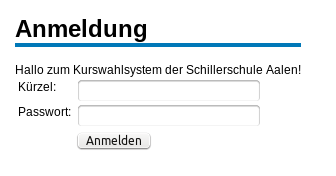
\includegraphics[scale=0.7]{img/login_KuWaSys.png}
 \end{center}
 \caption[\textbf{KuWaSys: Login Maske und Startseite}]{KuWaSys: Login Maske und Startseite}
 \label{fig:login_KuWaSys}
\end{wrapfigure}


Für den Vorgang des Logins am System besitzt der Servlet-Container Tomcat 7 eine sehr hilfreiche und gängige Funktion der Softwareentwicklung, die Konfiguation des \ac{DBCP}s des Apache Commons Projekts. Nähere Informationen sind unter \cite{ApacheDBCP} zu finden. 

Wie bereits aus dem \prettyref{subsec:Datenbankmodellierung} bekannt ist, haben wir für unser Datenbank eine zusätzliche Tabelle 'Rolle', die mit der Tabelle 'User' in Relation steht, modelliert. Diese wird nun für die Konfiguration des \ac{DBCP}s benötigt.

Der \ac{DBCP} gehört zu einer Art

Aufgrund der Tatsache, dass die Rollen-Tabelle mit der User-Tabelle in einer Beziehung zueinander steht, kann bei der Authentifizierung also genau auf den gewollten User zugegriffen werden. Diese Tatsache machen wir uns auch im weiteren Verlauf der Systemimplementierung zu Nutze, bspw. bei der Generierung von Benutzerdaten (\prettyref{subsec:Daten eines Benutzers}) oder aber um Daten zu manipulieren die mit dem User in Verbindung stehen.

%%
\todo[size=\small, color=orange!40]{Datenbankabfrage und Check Methoden Listing}
%%
 

\subsection{Benutzerverwaltung}\label{subsec:Daten eines Benutzers}
%%
\todo[size=\small, color=red!40]{Eindeutigkeit von Usernamen/Passwort bei Generierung}
%%

\subsubsection{Anlegen von Benutzerdaten}

Das Anlegen eines Benutzers erfordert immer die Informationen über:
\begin{itemize}
  \item Vor- und Nachname
  \item Geburtsdatum
  \item Klasse
  \item Konfession
\end{itemize}

Die Rolle, die ein Benutzer im System erhält, wird durch zwei unterschiedlich Eingabeaufforderungsdesigns umgesetzt. Eines für Lehrer und eines für Schüler. Benutzernamen und Passwörter werden vom System anhand der eingegebenen Informationen automatisch generiert. 

% User anlegen: Schüler
\begin{figure}[H]
 \begin{center}
   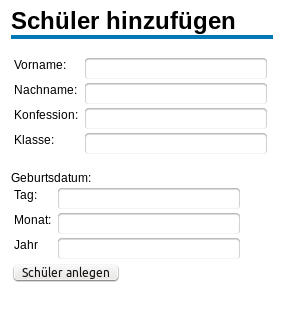
\includegraphics[scale=0.6]{img/UserAnlegen_KuWaSys.png}
 \end{center}
 \caption[\textbf{KuWaSys: User anlegen}]{KuWaSys: User anlegen}
 \label{fig:UserAnlegen_KuWaSys}
\end{figure}


% User anlegen: Lehrer
\begin{figure}[H]
 \begin{center}
   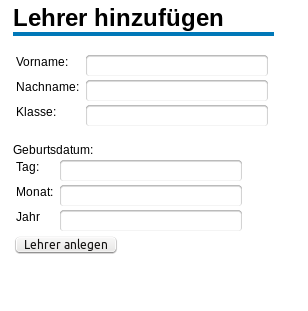
\includegraphics[scale=0.6]{img/LehrerAnlegen_KuWaSys.png}
 \end{center}
 \caption[\textbf{KuWaSys: Lehrer anlegen}]{KuWaSys: Lehrer anlegen}
 \label{fig:LehrerAnlegen_KuWaSys}
\end{figure}

textbf{Sonderfunktion: CSV-Import}

Eine Besonderheit der Benutzerverwaltung ist der Import von Userdaten über \ac{CSV}-Dateien. Diese Funktion war im Sinner der Projektarbeit nicht gefordert erleichtert aber die Arbeit mit dem System ungemein. Da jedes Jahr, zum Schuljahresbeginn, neue Schüler in das Kursplanungs- und Kurswahlsystem mit aufgenommen werden müssen wäre der Aufwand einzelne Benutzer hinzuzufügen zu groß und langwierig. Außerdem werden CSV-Dateien auch von gängigen Tabellenkalkulationsprogrammen unterstützt.

Als Vorlage für erste Importversuche diente die aktuelle Schülerliste im CSV-Format. Diese enthielt Daten in der Form:
%% Listing: CSV Schüler
	\lstinputlisting[label={lst:schiller_schueler.csv},
	caption={Beispiel einer CSV-Datei mit User Informationen},
	frame=tlbr, 
	language=java, 
	breaklines=true, 
	numbers=left, 
	numberstyle=\tiny, 
	stepnumber=1, 
	numbersep=5pt, 
	basicstyle=\small\ttfamily,
	showstringspaces=true,
	keywordstyle=\bfseries\color{lila}, 
	backgroundcolor=\color{lightgrey}]{listings/schiller_schueler.csv}

Mit Hilfe dieser Datei konnte ein Parser entworfen werden. Umgesetzt wurde der Parser mit der JAVA-Klasse \texttt{StringTokenizer}, um Tokens zu definieren und nach ihnen zu selektieren, und mit der Klasse \texttt{BufferedReader} und \texttt{InputStreamReader}, um die CSV-Datei überhaupt erst einlesen zu können. 

Der \prettyref{lst:ImportBean.java} zeigt die ManagedBean-Klasse \texttt{importBean} mit der Methode \texttt{doImport()}, die den komplettem Parse-Vorgang einer CSV-Datei steuert.
Die wichtigsten Zeilen des Quellcodeausschnitts sollen kurz erläutert werden:
\begin{itemize}
  \item[Zeile]
  \item[08:] Initialisierung der String-Variablen
  \item[23:] Beginn des Parsing-Vorgangs: Solange die CSV-Datei weitere Zeilen enthält
  \item[25:] Initialisierung des StringTokenizers (Zeilen und Angabe des Trennzeichens)
  \item[26:] Zeilenweise Tokens auswählen, solange weitere Tokens existieren
  \item[28:] Switch-Case fängt Integer-Wert der Tokens ab und weist die Werte den richtige Strings zu
  \item[47:] Aufruf der Methode \texttt{addUser} der \texttt{DatabaseHandler}-Klasse, die als Paramter die ausgelesenen Informationen der CSV-Datei enthält und einen neuen User im System anlegt
\end{itemize}

Wie unschwer zu erkennen ist, ist der Parser sehr einfach gestrickt. Es reicht anzugeben welche Trennzeichen zwischen den Daten benutzt werden (Obwohl der Namen CSV als Trennzeichen das Komma suggeriert, können als Trennzeichen zumindest auch Semikoli verwendet werden).
Weiter ist es ausreichend zu wissen wann die CSV-Datei endet und schlussendlich wie die Reihenfolge, der Werte die ausgelesen werden sollen, ist.

%% Listing: CSV Schüler - Parser
	\lstinputlisting[label={lst:ImportBean.java},
	caption={CSV-Datei Parser-Methode},
	frame=tlbr, 
	language=java, 
	breaklines=true, 
	numbers=left, 
	numberstyle=\tiny, 
	stepnumber=1, 
	numbersep=5pt, 
	basicstyle=\small\ttfamily,
	showstringspaces=true,
	keywordstyle=\bfseries\color{lila}, 
	tabsize=2,
	backgroundcolor=\color{lightgrey}]{listings/ImportBean.java}

\subsection{Kursverwaltung}

Neben dem Anlegen von neuen Benutzern, muss das System auch die Funktionalität besitzen, neue Kurse hinzuzufügen.

%%
\todo[size=\small, color=red!40]{Kurs anlegen (Lehrer)/Kurs aktivieren (Admin)/Kurs wählen (Schüler) !!!auch Diagramm!!!}
%%

Darstellung des Stundenplans:
\begin{figure}[H]
\centering
\begin{tikzpicture}[x=\daywidth, y=-1cm, node distance=0 cm,outer sep = 0pt]
% Style for Days
\tikzstyle{day}=[draw, rectangle,  minimum height=1cm, minimum width=\daywidth, fill=yellow!20,anchor=south west]
% Style for hours
\tikzstyle{hour}=[draw, rectangle, minimum height=1 cm, minimum width=1.5 cm, fill=yellow!30,anchor=north east]

% Styles for events
% Dauer Stunden
\tikzstyle{hours}=[rectangle,draw, minimum width=\daywidth, anchor=north west,text centered,text width=5 em]
\tikzstyle{1hour}=[hours,minimum height=1cm]
\tikzstyle{2hours}=[hours,minimum height=2cm]
\tikzstyle{3hours}=[hours,minimum height=3cm]

% Style der Fächer
\tikzstyle{Kern}=[2hours,fill=green!20]
\tikzstyle{Kurs1}=[2hours,fill=red!20]
\tikzstyle{Kurs2}=[2hours,fill=blue!20]
\tikzstyle{Kurs3}=[2hours,fill=blue!10]
\tikzstyle{Kurs4}=[2hours, pattern=north east lines, pattern color=magenta]
\tikzstyle{Kurs5}=[3hours, pattern=north west lines, pattern color=magenta!60!white]s
\tikzstyle{Planche}=[1hour,fill=white]

% Positioning Tag/Stunden
\node[day] (mo) at (1,8) {Montag};
\node[day] (di) [right = of mo] {Dienstag};
\node[day] (mi) [right = of di] {Mittwoch};
\node[day] (do) [right = of mi] {Donnerstag};
\node[day] (fr) [right = of do] {Freitag};

\node[hour] (8-9) at (1,8) {8-9};
\node[hour] (9-10) [below = of 8-9] {9-10};
\node[hour] (10-11) [below= of 9-10] {10-11};
\node[hour] (11-12) [below = of 10-11] {11-12};
\node[hour] (12-13) [below  = of 11-12] {12-13};
\node[hour] (13-14) [below = of 12-13] {13-14};
\node[hour] (14-15) [below = of 13-14] {14-15};
\node[hour] (15-16) [below = of 14-15] {15-16};
\node[hour] (16-17) [below = of 15-16] {16-17};
\node[hour] (17-18) [below = of 16-17] {17-18};
\node[hour] (18-19) [below = of 17-18] {18-19};

% Position Fächer
\node[Kurs1] at (1,10) {Sport};
\node[Kern] at (1,8) {D/M/E};
\node[Kern] at (2,8) {Physique};
\node[Kern] at (4,8) {Physique};
\node[Kern] at (5,10) {Physique};
\node[Kern] at (2,10) {Maths};
\node[Kern] at (2,14) {Maths};
\node[Kern] at (3,8) {Maths};
\node[Kern] at (4,10) {Maths};
\node[Kern] at (5,8) {Maths};
\node[Kern] at (1,14) {TIPE};
\node[Kern] at (1,16) {TIPE};
\node[Kern] at (2,16) {TIPE};
\node[Kern] at (3,10) {TIPE};
\node[Kern] at (5,14) {TIPE};
\node[Kern] at (5,16) {TIPE};
\node[Kern] at (3,14) {Phys ou SI};
\node[Kern] at (3,16) {SI ou Phys};
\node[Kern] at (1,13) {Planche};
\node[Kern] at (1,18) {Colle};
\node[Kern] at (4,13.5) {Planche};

\end{tikzpicture}
\caption[\textbf{Netzwerkstruktur der Schillerschule Aalen}]{Netzwerkstruktur der Schillerschule Aalen}
\label{fig:Stundenplan}
\end{figure}

\subsubsection{Spezielle Daten eines Kurses}

Der Aufbau eines Kurses im System, wie aus dem ER-Modell in \prettyref{fig:ERModell} entnommen werden kann, besteht im Grunde aus einer Nummer, einem verantwortlichen Lehrer, einer Beschreibung, einem Termin, Information des dazugehörigen Fächerverbunds  und einer Teilnehmeranzahl. Allein mit diesen Information könnte ein Kurs im System dargestelltn werden. Hierbei werden jedoch die restlichen Attribute vernachlässigt. Diese sollen im folgenden näher zur Sprache kommen.  

Da die angebotenen Kurse im System nun verschiedenen Abhängigkeiten haben können und eventuell bestimmte Vorraussetzungen erfüllen können müssen, wurde eine Möglichkeit gesucht diese Kurse möglichst einfach im System abzubilden. 
Einfach bedeutet an dieser Stelle, dass die Darstellung eines Kurses für alle Rollen gleichermaßen zur Verfügung stehen muss und außerdem Interaktionen mit ihnen unterstützt.
Hierbei müssen die oben vernachlässigten Attribute beachtet werden. 

Attribute die hierbei einer Rolle spielen sind: (Vrgl. ER-Modell in \prettyref{subsec:ERModell})
\begin{itemize}
  \item Sportkurs
  \item Konfession (derzeit EV, RK und Ethik)
  \item Pflichtkurse
\end{itemize}

\textbf{Sportkurse}

Hierbei handelt es sich um ein Attribut, also einer Spalte in der Kurs-Tabelle, die den Datentyp \texttt{boolean} besitzt.
Beim Anlegen hat der Lehrer oder der Admin die Möglichkeit dieses Attribut des zu erstellenden Kurses zu setzen, wie es die grüne Markierung in \prettyref{fig:KursAnlegen_KuWaSys} zeigt.

Das anlegen des Sportkurs-Flags in der DB ist trivial und wird daher nicht weiter betrachtet.

Von einer Besonderheit bei Sportkursen kann gesprochen werden wenn zusätzlich die Fächerverbünde und Pflichtkurse mitbetrachtet werden.
Für gewöhnlich wird ein Sportkurs dem Fächerverbund \ac{MSG} zugeordnet. Es kann allerdings vorkommen, dass ein Kurs als Sportkurs angelegt wird, aber keinen Pflichtkurs darstellt.  
Pflichtkurse werden am Ende dieses Abschnitts noch behandelt.

Beim Anlegen hat der Lehrer oder der Admin die Möglichkeit dieses Attribut des zu erstellenden Kurses zu setzen, wie es die grüne Markierung in \prettyref{fig:KursAnlegen_KuWaSys} zeigt.


\textbf{Religionsunterricht}

Eine richtige Besonderheit stellt das Anlegen eines Religionskurses dar.
Das Anlegen eines Religionskurses (grüne Markierung in \prettyref{fig:KursAnlegen_KuWaSys}) wird über einfach Selectboxen realisiert. Der Inhalt der Selectboxen wird dazu automatisch angelegt. Wie dies gewährleistet wird soll nun näher besprochen werden.

Wie bereits in \prettyref{fig:UserAnlegen_KuWaSys} gezeigt wurde, wird beim Anlegen eines Users im System, eine Konfessionszugehörigkeit beigefügt. Dieses Feld kann vom Admin beliebig ausgefüllt werden. 
Dieser beliebige String wird in die Tabelle 'Kurskonfession' eingetragen und wird später, durch die Auswahl beim Anlegen eines Kurses, als Fremdschlüssel in der 'Kurs'-Tabelle gespeichert.
Der Inhalt der Selectboxen die zur Verfügung stehen, ist also immer komplette Inhalt der Kurskonfession-Tabelle.




Diese Art der Lösung soll in Zukunft alternative Unterrichte zulassen können.

% Kurs anlegen
\begin{figure}[H]
 \begin{center}
   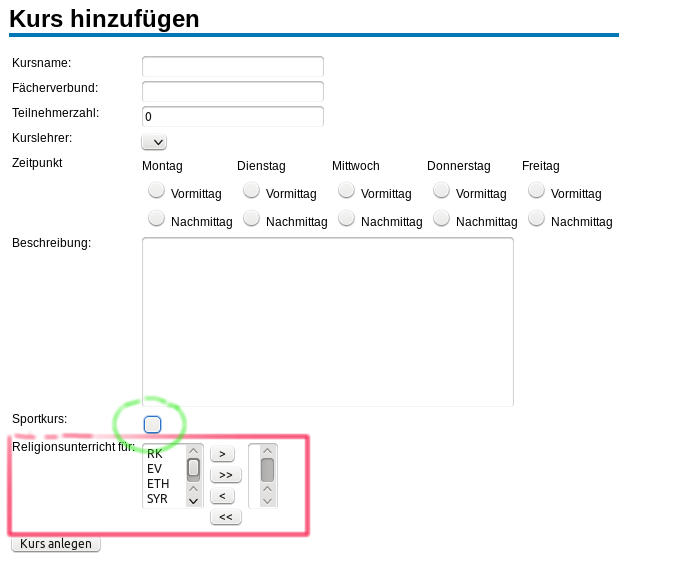
\includegraphics[scale=0.6]{img/KursAnlegen_KuWaSys.png}
 \end{center}
 \caption[\textbf{KuWaSys: Kurs anlegen}]{KuWaSys: Kurs anlegen}
 \label{fig:KursAnlegen_KuWaSys}
\end{figure}

\textbf{Pflichtkurse}

Ähnlich wie bei Sportkursen handelt es sich hierbei um ein Attribut, also ebenfalls einer Spalte in der Kurs-Tabelle, die auch den Datentyp \texttt{boolean} besitzt.
Im Gegesatz zu Sportkursen wird das Pflichtkurs-Flag allerdings nicht beim Anlegen eines Kurses gesetzt. Es kann nur vom Admin bestimmt werden, ob ein Kurs ein Pflichtkurs ist oder nicht. Festlegen kann er dies in der Kursverwaltung in der Phase der Kursplanung.

Die \prettyref{fig:KursVerwalten_KuWaSys} zeigt einen Ausschnitt der Kursverwaltung aus Sicht des Admins.
Der Admin hat die Möglichkeit Kurse zu aktivieren, also den Schülern die Kurse zur Kurswahl zur Verfügung zu stellen oder bereits aktivierte Kurse wieder zu deaktivieren.
Darüberhinaus legt der Admin die Pflichtkurse fest.

% Kurs verwalten
\begin{figure}[H]
 \begin{center}
   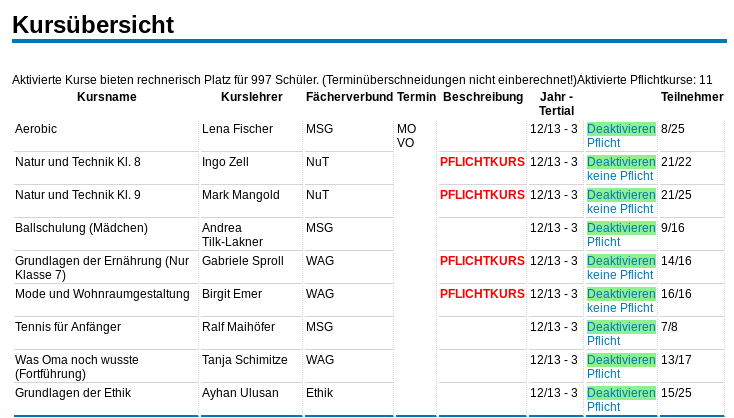
\includegraphics[scale=0.6]{img/KursVerwalten_KuWaSys.png}
 \end{center}
 \caption[\textbf{KuWaSys: Kurse verwalten}]{KuWaSys: Kurse verwalten}
 \label{fig:KursVerwalten_KuWaSys}
\end{figure}

\subsubsection{Benutzerunterstützung}
%%
\todo[size=\small, color=red!40]{Anzeige der abgehandelten Kurse/Fächerverbünde etc... (Schüler bzw. Admin)}
%%%%
\todo[size=\small, color=orange!40]{Screenshot}
%%


\subsection{Systemverwaltung}
%%
\todo[size=\small, color=red!40]{Umsetzung der Stati des Systems}
%%%%
\todo[size=\small, color=orange!40]{Screenshot}
%%



\section{Tests, Fehlervermeidung und Qualitätssicherung}\label{sec:Testing und Debugging}

%% Einleitung %(
Dieser Abschnitt widmet sich dem Thema der Testverfahren in Softwareprojekten mit dem Schwerpunkt bezogen auf das entwickelte JSF-Projekt 'KuWaSys'.
Zuerst sollen die allgemein geltenden Grundlagen angesprochen werden, darauf aufbauend werden die im Projekt verwendeten Testverfahren näher erläutert. 

Tests lassen sich in der Software Entwicklung nach ihrer Art und Weise klassifizieren.
Auf der einen Seite steht die Konstruktive-Qualitätssicherung auf der anderen Seite die Analytische.

Zu den Konstruktiven-Qualitätssicherungsmaßnahmen zählen Durchführungen während dem und am Entwicklungsprozesses selbst:
\begin{itemize}
  \item Checklisten
  \item Programmier-Guidlines
  \item Templates
\end{itemize}

Die Analytischen-Qualitätssicherung, zu welchen Tests am Produkt gehören, können in zwei verschiedene Testverfahren eingeteilt werden. Hierbei handelt es sich um statische und dynamische Tests.
Verfahren die hierzu eingesetzt werden sind für statische Test:
\begin{itemize}
  \item Statische Analyse
  \item Reviews
\end{itemize}

Im Sinne der statischen Analyse wurden während der Entwicklung folgende Punkte überprüft:
\begin{itemize}
  \item existieren Klassen bzw. Methoden
  \item sind die Scopes der ManagedBeans korrekt
  \item sind ManagedBeans mit dem Scope \texttt{Session} und \texttt{Application} serialisierbar
  \item haben ManagedBeans Properties die benötigten Setter-/Getter-Methoden
\end{itemize}

Und für dynamische Test beispielsweise:
\begin{itemize}
  \item \gls{Blackbox}-Testverfahren
  \item \gls{Whitebox}-Testverfahren
\end{itemize}


Die Planung und Strukturierung der Durchführung von Softwaretests, aber auch die Überlegung von Testfällen die am System geprüft werden sollen, stellen einen äußerst wichtigen Prozess der Softwareentwicklung dar.
Diese Schritte fließen bestenfalls zu Beginn des Projekts, in der Planungsphase, mit ein. (\cite{SPM}, ab Seite 5undzwölfzig)

%% TODO evtl hier checkliste?!
Als geplante Tests am fertigen System wurden die folgenden vorgesehen, die im Checklisten-Verfahren abgearbeitet wurden:
\begin{itemize}
	\item Tests bezügliche der Interaktion am System (mit Testpersonen und deren Feedback)
	\begin{itemize} 
		 \item prüfen der Übersichtlichkeit aller Benutzergruppen
		 \item Kontrolle des Seitenaufbaus und der Strukturierung für effizientes Arbeiten
	\end{itemize}
	\item Testeingaben in Textfelder
	\begin{itemize} 
		 \item Tests der Schnittstellen und der übergebenen Parameter nach Datentyp
		 \item Abklärung von eventuellen Encoding-Problemen
	\end{itemize}
	\item Funktionalitätstests aller Schaltflächen
	\begin{itemize} 
		 \item absichern von korrekten Systemereignissen bzw. -funktionen
		 \item Kontrolle der übergebenen Werte und Datentypen, um Fehlbelegungen auszuschließen
	\end{itemize}
	\item Konsistenz der Datenbank 
	\begin{itemize} 
		 \item Abfragen mit Hinblick auf Eindeutigkeit, bspw. bei \texttt{UNIQUE-Constraints} sowie \texttt{PRIMARY KEY-} und \texttt{FOREIGN KEY-Constraints}
		 \item Überprüfung der verwendeten Datentypen im System
	\end{itemize}
\end{itemize}

Im folgenden sollen Tests im Zusammenhang mit der Softwarequalitätssicherung und die Umsetzung im 'KuWaSys' näher betrachtet werden.

Der Stellenwert der Qualitätssicherung von Software hat in der heutigen Zeit einen so großen Stellenwert angenommen, dass es mittlerweile sogar ISO-Normen gibt, genauer gesagt die ISO-Norm 9126 - für Qualität in Software. Diese Norm enthält grundlegende Bestimmungen über Effizienz, Funktionalität, Zuverläsigkeit, Benutzbarkeit, Portabilität und Wartbarkeit. 
Die genauen Details der Definitionen werden hier nicht weiter erwähnt da diese über das Thema der Projektarbeit hinaus gehen würden. Eine gute und vollständige Zusammenfassung der gesamten Norm ist jedoch unter \cite{WikiISO9126} zu finden.

% ISO 9126 MindMap
\begin{figure}[H]
\centering\begin{tikzpicture}[mindmap,
  level 1 concept/.append style={level distance=130,sibling angle=30},
  extra concept/.append style={color=blue!50,text=black}]

\begin{scope}[mindmap, concept color=green, text=white]
\node [concept]at (-2,1) {ISO 9126}[clockwise from=-5]
    child [grow=10] {node [concept] (E) {Effizienz}}
    child {node [concept] (F) {Funktionali-tät}}
    child [grow=240] {node [concept] (E) {Zuverläsig-keit}}
    child [grow=110] {node [concept] (B) {Benutzbar-keit}}
    child [grow=60] {node [concept] (P) {Portabilität}}
    child [grow=280] {node [concept] (W) {Wartbarkeit}};
\end{scope}
\end{tikzpicture}
\caption[\textbf{ISO Norm 9126}]{ISO Norm 9126}
\label{fig:Projekt_Mindmap}
\end{figure}
%)

%% Test/Qualität im Projekt %(
Grundsätzlich wurden allgemein gültige Richtlinien und Code-Konventionen von JSF im Projekt umgesetzt. Dies erhöht zum eine die Übersichtlichkeit des gesamten Projekts und wirkt sich postiv auf die kooperierende Entwicklung aus. Dadurch werden gleichermaßen qualitätsichernde Maßnahmen ergriffen wie auch Fehleranfälligkeiten minimiert.  

Das Benutzen von Templates, welche während der Implementierungsphase eingesetzt wurden, stellt ebenfalls eine Technik dar, die zur Fehlervermeidung beiträgt. Das verwendete Design des 'KuWaSys' musste somit nur einmal definiert und getestet werden und konnte anschließend beliebig oft weiter verwendet werden ohne dabei das Risiko eingehen zu müssen dass das Design inkonsistent wird oder dass sich neue Fehler im Projekt einschleichen könnten. 

Um Laufzeittests durchzuführen wurden FacesMessages, über den entsprechenden Import der Klasse \texttt{javax.faces.application.FacesMessage} benutzt, die Gleichzeitig die Fehleranalyse mit Hilfe der Konsole erleichtern.
Ein Beispiel solcher Messages ist in \prettyref{lst:FacesMessages} dargestellt. Im Falle eines Fehlers würde der ausgeführte \texttt{Catch}-Block, über den benutzerdefinierten FacesMessages-Befehl, eine Ausgabe produzieren.
Nebenbei sei noch eine weitere Besonderheit in JSF angemerkt:
Während der Status 'Development' im  Projekt steht, welcher in der \texttt{POM.xml} festgelegt wird, werden Fehler für bestimmte Funktionen automatisch ausgegeben. Dies ist vor allem bei einem Release zu beachten und vorher abzuändern.

%% Listing: FacesMessages
	\lstinputlisting[label={lst:FacesMessages},
	caption={Debugging mit FacesMessages},
	frame=tlbr, 
	language=java, 
	breaklines=true, 
	numbers=left, 
	numberstyle=\tiny, 
	stepnumber=1, 
	numbersep=5pt, 
	basicstyle=\small\ttfamily,
	showstringspaces=true,
	keywordstyle=\bfseries\color{lila}, 
	tabsize=2,
	backgroundcolor=\color{lightgrey}]{listings/FacesMessages.java}
	
Wie in der folgenden \prettyref{figmin:SchulerImportieren_KuWaSys} zu erkennen ist, wird die Message während der Laufzeit ausgeführt, wie bei diesem missglückten Datei-Upload.

% Kurs anlegen
\begin{figure}[H]
 \begin{center}
   
\includegraphics[scale=0.8]{img/SchulerImportieren_KuWaSys.png}
 \end{center}
 \caption[\textbf{KuWaSys: Datei-Upload Fehler beim Schüler Importieren}]{KuWaSys: Datei-Upload Fehler beim Schüler Importieren}
 \label{figmin:SchulerImportieren_KuWaSys}
 \label{fig:SchulerImportieren_KuWaSys}
\end{figure}

Diese Tests erwiesen sich bei Datenbankabfragen als sehr hilfreich, da nicht erst aufwändige Oberflächen umgesetzt werden müssen um Fehler zu erkennen, sondern Daten sofort auf ihre Richtigkeit hin geprüft werden können.
Diese Fehler sind gleich zu Beginn der Implementierung aufgefallen, da es sich hier vor allem um Fehler die während der Modellierungs- beziehungsweise (bzw.) Designphase entstanden sind, handelt. Diese Fehler sind mit FacesMessages relativ schnell auszumachen und ebenso schnell korrigiert. Beispiele solcher Fehler sind:
\begin{itemize}
  \item falsche Überlegungen zu den Datentypen in der \ac{DB}
  \item schlecht definierte Schnittstellen
  \item Inkonsitenz im Design 
\end{itemize}

Eine weitere Möglichkeit, Fehler in einer Webapplikation zu entdecken ist das benutzen von selbstdefinierten Server-Logs.
Hierzu wurde von uns die Klasse \texttt{import java.util.logging.Logger} verwendet. Der \prettyref{lst:Logger} zeigt wie beispielsweise ein \texttt{Catch}-Block  mitgeloggt werden kann.

%% Listing: Logging
	\lstinputlisting[label={lst:Logger},
	caption={Server-Logging in JSF},
	frame=tlbr, 
	language=java, 
	breaklines=true, 
	numbers=left, 
	numberstyle=\tiny, 
	stepnumber=1, 
	numbersep=5pt, 
	basicstyle=\small\ttfamily,
	showstringspaces=true,
	keywordstyle=\bfseries\color{lila}, 
	tabsize=2,
	backgroundcolor=\color{lightgrey}]{listings/Logger.java}

Da ständig auf einem aktiven System (Corporate Identity) - glossarntwickelt und getestet wurde konnten Tester aus dem Umfeld der Schule für diesen Zweck eingesetzt werden.
Dies erwies sich vor allem beim Entwickeln des Oberflächendesigns als Vorteil. Es konnten Wünsche von Lehrern und Schülern direkt berücksichtigt und umgesetzt werden.
Hier bekommen besonders Checklisten und Reviews einen hohen Stellenwert. Nur durch regelmäßige gemeinsame Treffen konnten Projekttermine (neu-)definiert werden.

Im Hinblick auf die vorher besprochene ISO-Norm 9126 erfüllt das Kurswahlsystem alle Bestimmungen. Jedoch muss fairnesshalber dazu gesagt werden, dass Dinge wie Effizienz in Software nie mit einem genauen Maß gemessen werden kann, da viele Faktoren ein Rolle spielen.
Zum Beispiel müssen bei gewissen Datenstrukturen Laufzeiteinschränkungen in Kauf genommen werden wenn sich dadurch die Darstellung effizienter umsetzen lässt. Andererseits können natürlich schneller Datenstrukturen oder Algorithmen in einer viel langsameren Darstellung resultieren.
Dasselbe gilt für die Zuverläsigkeit. Natürlich ist das Kurswahlsystem so entworfen worden, dass die Erreichbarkeit und Nutzbarkeit jederzeit gegeben ist. Aber auch hier unterliegt das System mehreren außenstehenden Faktoren auf die ein Entwickler niemals Einfluss nehmen kann.
%)

%% JSFUnit %(
Selbstverständlich können für den Java Server Faces Standard auch Tests implementiert werden. Diese werden für gewöhnlich bei den Dynamischen-Test angesiedelt. Von uns wurden keine spezielle Frameworks zur Realisierung von Tests verwendet. Vollständigkeitshalber soll allerdings eines der interessantesten Vertreter von Testinstrumenten für JSF erwähnt werden:

Hierbei handelt es sich um \gls{JSFUnit}, welches auf dem bekannten JAVA-Testframework \gls{JUnit} aufbaut. Tests können hierzu über die JSFUnit-Konsole oder durch den Aufruf einer Testseite ausgeführt werden. Testmöglichkeiten sind Wert- und Zustandsänderungen in ManagedBeans, setzen von Navigationszielen oder über FacesMessages.
Eine besondere Art der Tests sind die 'Acrylic Box'-Testings. Diese verbinden Whitebox und Blackbox-Testverfahren und werden bei den dynamischen Tests eingestuft.
Nähere Informationen sind unter \cite{JSFUnit01} zu finden.
%)

Zuletzt soll noch hinzugefügt werden, dass auch ausführliche Tests keine Garantie auf eine vollständige Fehlerfreiheit geben.
Allerdings helfen Tests die Fehler möglichst gering zu halten und steigern die Qualität der Software um ein gewisses Maß.
Obwohl das Projekt ausführlichst getestet wurde kann es dennoch nicht ausgeschlossen werden, dass noch welche existieren. 

\newpage

\section{Fazit und Ausblick}\label{sec:Fazit und Ausblick}

%% Einleitung %(
Abschließend soll ein gesamtheitlicher Überblick der Projektarbeit gegeben werden, indem das entwickelte System komplett betrachtet wird.
Für ein sinnvolles Fazit sollen zwei wesentliche Punkte angesprochen werden:
\begin{enumerate}
  \item Beurteilung der Nutzbarkeit und die gesamtheitliche Umsetzung des Projekts
  \item Beurteilung der eingesetzten Technologien
\end{enumerate}

%%% TODO
Vor allem beim zweiten Punkt sollen zwei weitere Kriterien differenziert werden:
Beim Einen handelt es sich um das Kriterium der Verwendbarkeit der Technologie für den Entwickler, hier ist dieser in einer aktiven Rolle zu sehen. 
Beim Anderen handelt es sich vor allem um eine Betrachtung der Technologie in Punkten wie Komplexität, Verwendbarkeit und Spezifiktaion, in welchen der Entwickler lediglich nur eine passive Rolle einnehmen kann.
%)

%% Betrachtung System %(
An oberster Stelle stand das Ziel, die Anforderungen an das System erfolgreich umzusetzen.
Das positive Resultat kann der engen Kooperation während der Implementierungsphase und der ausgiebigen Problemabgrenzung, wie grob zu Beginn in \prettyref{subsec:Problemstellung und -abgrenzung} beschrieben ist, angerechnet werden.
Vor allem die ersten drei bis vier Wochen nach Projektstart dienten dazu, die Ziele zu definieren. Beinahe jede Woche hielten wir mit den verantwortlichen Personen (in \prettyref{subsec:Verantwortliche Personen} namentlich aufgeführt) der Schillerschule Aalen ein Projektmeeting ab, in welchem Ergebnisse des Projektfortschritts präsentiert und diskutiert wurden.
Ein weiterer wichtiger Punkt, der zu diesem Ergebnis geführt hat, war das entgegengebrachte Vertrauen von Seiten der Schule.

Wie es \prettyref{secmin:Implementierung} zu entnehmen ist, wurden alle Punkte der Systemanforderung erfüllt. Darüberhinaus wurden sogar zusätzliche Funktionalitäten implementiert.
Hier wäre die Umsetzung der Export-/Importfunktionen von CSV Dateien, Funktionalität die Userdaten betreffen (bspw. Passwort-Neugenerierung) und die komplette Umsetzung der \ac{IT}-Infrastruktur der Schillerschule genannt. 
Insofern muss der entstandene Fortschritt mit dem neuen Kurswahlsystem im Hinblick auf das erste Kursverwaltungstool gesehen werden.

Das größte Manko, der nicht unterstützte Multi-User Betrieb und die Einschränkung der Lauffähigkeit begrenzt auf ein System, wurden beseitigt. Ebenso wurde mehr Wert auf ein gewisses Maß an Selbstverantwortung bei Lehrern aber auch Schülern gelegt.
Im Idealfall wird der Admin nur noch zur Konfiguration des Systems und in Problemfällen aktiv.
Auch die Verwaltungsassistenz wurde im neuen Tool erfolgreich umgesetzt. So werden Daten die für die Kursplanung wichtig sind vom System ermittelt und den Benutzern zur Verfügung gestellt. 
Ebenso wurde der entwickelte Arbeitsablauf für Lehrer und Schüler umgesetzt und die Kommunikation untereinander dadruch verbessert indem Probleme Systembedingt abgefangen werden können.

Als dritter und letzter Verbesserungsschritt ist die neugestaltung der Oberfläche zu sehen. Diese wurden mit Hilfe von bereits erprobten und bewährten Gestaltungselementen, die aus dem Gebiet der \ac{MCI} bekannt sind, umgesetzt. \cite{DahmMCI}.

Die eindeutige Abgrenzung von Menü, Informationen und Arbeitsbereich sind gleichermaßen umgesetzt wie die Darstellung aller Systemrelevanter Daten wie es in der Anforderung gewünscht war.

Zukünftige Erweiterungen sind im System vorgesehen. Aufgrund der Modularität die sich strikt durch das ganze System zieht werden diese auch realisierbar sein.

Realisierbare Erweiterungen könnten sein:
\begin{itemize}
  \item eine Änderungsinformationsanzeige für Admins bei bestimmten Systemereignissen, sodass ohne fundierte \ac{IT}-Kenntnisse, Fehler an Server und Datenbank frühzeitig erkannt werden können
  \item eine interne Kommunikationsplattform für den Austausch von Informationen zwischen Lehrern und Administrator und zwischen Schülern - und Lehrern  
  \item Erweiterungen wie Kalenderfunktionen, Stundenplan-Generierung,....
\end{itemize}
  
Manche der aufgeführten Vorschläge werden bereits im Momentanen Stand der Entwicklung, ansatzweise umgesetzt. 
Aufgrund der Fülle und Diversität der Art an Anforderungen die zu Beginn an das Projekt festgehalten wurden fanden diese jedoch in der Projektarbeit bedauerlicherweise fast keinen Platz.
%)

%% Technologien %(
Es hat sich gezeigt, dass \ac{JSF} ein gut definierter Webentwicklungsstandard geworden ist.
Aufgrund der Einfachheit der Handhabung kommen Anfänger der Webentwicklung aber auch Fortgeschrittene gut damit zurecht und voll auf ihre Kosten.
Je nach Komplexität der Interaktion mit dem System sind JAVA Kenntnisse erfoderlich, in jedem Falle aber sinnvoll. 
Eine Entwicklung die ihren Schwerpunkt auf das Design oder generell die Darstellung legt benötigt nur sehr wenige Kenntnisse im Bereich JAVA dafür aber Kenntnisse einer Seitendeklarationssprache wie HTML oder JSP.
Sollen aber, wie es in dieser Projektarbeit der Fall war, Daten aus einer Datenbank verändert oder in eine Datenbank geschrieben werden sind fundierte Kenntnisse der Softwareentwicklung mit JAVA notwendig.

Zur verwendeten Datenbank lassen sich keine besonders wichtigen oder bahnbrechenden Aussagen machen. PostgreSQL hat sich bereits über Jahre etabliert und wurde stetig weiter verbessert. 
Die Verwendung für unerfahrene Nutzer stellt nach einer kurzen Einarbeitung kein größeres Problem dar und kann somit nur weiterempfohlen werden. 
 
Die Entwicklungsunterstützung mit Maven ist bei Projekten dieser Art eine sehr große Hilfe.
Ohne eine Verwaltungshilfe der Bibliotheken, Pakete oder der Projektverweise kann ein Projekt in dieser Größenordnung schnell in einen Bereich kommen, in welchem plötzlich der Verwaltungsaufwand steigt und schnell zur Hauptaufgabe des Entwicklers wird.
Der Fokus schweift immer öfters vom Projekt ab. Das Resultat davon ist:
\begin{itemize}
	\item ein höherem Zeitaufwand für das Beheben von entstandenen Problemen durch die Verletzung von Abhängigkeiten 
	\item mehr Fehler im Programmcode der wiederrum auch zu längeren Testphasen führt
	\item teilweise leidet die Qualität des entstanden Codes 
\end{itemize}
Für viele Entwickler (oder Projektleiter) ist dies ein stark vernachlässigtes Thema.
Ohne eine genaue Planung und ohne konkrete Vorstellungen lässt sich jedoch ein Softwareprojekt, egal welcher Größe, meist nie korrekt realisieren.  
Dies sind alles Gründe die dafür gesorgt haben, dass das Projekt unter zu Hilfenahme des Development-Tools Maven umgesetzt wurde.
Die Softwareentwicklung bleibt im Vordergrund.
%)

%% Rückblick %(
Rückblickend kann dem Projekt ein voller Erfolg zugeschrieben werden.
Funktional genügt das System den Anforderungen und sogar darüber hinaus. Der zeitliche Aufwand war sehr hoch, aber im Rahmen des Möglichen, sodass nicht von 'zu viel' gesprochen werden kann.
Zeitliche Einbußen musste dennoch hingenommen werden. So stellten vor allem das Testen und die Integration des Systems in die Infratruktur der Schule einen langwierigen Prozess dar und sprengte den geplanten Rahmen.
Letztenendes sorgten Dinge wie die Anleitung, die technische Dokumentation und diese Ausarbeitung der Projektarbeit für den nötigen Abschluss des Projekts.

%)

\newpage

%% Neuer Style
\pagestyle{fancy}
	\renewcommand{\sectionmark}[1]{\markboth{#1}{}}
	\fancyhf{}
	\fancyhead[L]{ { }\leftmark}
	\fancyhead[R]{\thepage}
	\renewcommand{\headrulewidth}{0.4pt}
	%\pagenumbering{roman}

Die ist in \prettyref{sec:Anhang} zu finden.
	
\begin{appendix}
\section{Anhang}\label{sec:Anhang}

\subsection{Inhalte der CD}
Folgende Inhalte sind auf der abgegebenen CD zu finden:

\begin{itemize}
  \item Kopie der Entwicklungsumgebung Eclipse 10.04 Juno mit allen Plugins
  \item virtuelles Abbild des konfigurierten Servers
  \item diese Ausarbeitung
  \item Dokumentation in JAVAdoc
  \item Benutzerhandbuch für das 'KuWaSys'				%%
  \item Kopien der verwendeten bzw. zitierten Websites\todo[size=\small, color=green!40]{Fragwürdig!!!} 
\end{itemize}											%%

\subsection{Konfiguration und Installation}

\subsubsection{Maven}

Maven Befehle listings

\subsubsection{Apache Tomcat 7}

Hier soll in einer kurzen Darstellung die Administration des Apache Tomcat 7 und dessen wichtige Dateien und Verzeichnisse 

\textbf{}
Apache Tomat7 Befehle Listings

Verzeichnisse

\subsection{Zugangsdaten für den Server und das System}

\textbf{Server Zugangsdaten}

% Zugangsdaten
\begin{table}[H]
\begin{center}
	\begin{tabular}{|l|l|l||}\hline
		\textbf{Rolle} & \textbf{Username} & \textbf{Passwort} \\ \hline
		Admin & ijcy & 12kuwasys34 \\ \hline \hline
	\end{tabular}
	\caption{Server Zugangsdaten}
\end{center}
\end{table}

\textbf{Datenbank Zugangsdaten}

% Datenbank Zugangsdaten
\begin{table}[H]
\begin{center}
	\begin{tabular}{|l|l|l||}\hline
		\textbf{Rolle} & \textbf{Username} & \textbf{Passwort} \\ \hline
		Admin & ijcy & 12kuwasys34 \\ \hline
		Admin & postgres & 12kuwasys34 \\ \hline \hline
	\end{tabular}
	\caption{Datenbank Zugangsdaten}
\end{center}
\end{table}

\subsection{Gesetzesauszüge}\label{subsec:Gesetz}

Auszug aus dem \ac{TMG}:

\textbf{§ 5 Allgemeine Informationspflichten}
\begin{itemize}
\item[(1)] Diensteanbieter haben für geschäftsmäßige, in der Regel gegen Entgelt angebotene Telemedien folgende Informationen leicht erkennbar, unmittelbar erreichbar und ständig verfügbar zu halten:
  \begin{enumerate}
    \item den Namen und die Anschrift, unter der sie niedergelassen sind, bei juristischen Personen zusätzlich die Rechtsform, den Vertretungsberechtigten und, sofern Angaben über das Kapital der Gesellschaft gemacht werden, das Stamm- oder Grundkapital sowie, wenn nicht alle in Geld zu leistenden Einlagen eingezahlt sind, der Gesamtbetrag der ausstehenden Einlagen,
    \item Angaben, die eine schnelle elektronische Kontaktaufnahme und unmittelbare Kommunikation mit ihnen ermöglichen, einschließlich der Adresse der elektronischen Post,
    \item soweit der Dienst im Rahmen einer Tätigkeit angeboten oder erbracht wird, die der behördlichen Zulassung bedarf, Angaben zur zuständigen Aufsichtsbehörde,
    \item das Handelsregister, Vereinsregister, Partnerschaftsregister oder Genossenschaftsregister, in das sie eingetragen sind, und die entsprechende Registernummer,
    \item soweit der Dienst in Ausübung eines Berufs im Sinne von Artikel 1 Buchstabe d der Richtlinie 89/48/EWG des Rates vom 21. Dezember 1988 über eine allgemeine Regelung zur Anerkennung der Hochschuldiplome, die eine mindestens dreijährige Berufsausbildung abschließen (ABl. EG Nr. L 19 S. 16), oder im Sinne von Artikel 1 Buchstabe f der Richtlinie 92/51/EWG des Rates vom 18. Juni 1992 über eine zweite allgemeine Regelung zur Anerkennung beruflicher Befähigungsnachweise in Ergänzung zur Richtlinie 89/48/EWG (ABl. EG Nr. L 209 S. 25, 1995 Nr. L 17 S. 20), zuletzt geändert durch die Richtlinie 97/38/EG der Kommission vom 20. Juni 1997 (ABl. EG Nr. L 184 S. 31), angeboten oder erbracht wird, Angaben über
    \begin{itemize}
      \item[a)] die Kammer, welcher die Diensteanbieter angehören,
      \item[b)] die gesetzliche Berufsbezeichnung und den Staat, in dem die Berufsbezeichnung verliehen worden ist,
      \item[c)] die Bezeichnung der berufsrechtlichen Regelungen und dazu, wie diese zugänglich sind,
    \end{itemize}
    \item in Fällen, in denen sie eine Umsatzsteueridentifikationsnummer nach § 27a des Umsatzsteuergesetzes oder eine Wirtschafts-Identifikationsnummer nach § 139c der Abgabenordnung besitzen, die Angabe dieser Nummer,
    \item bei Aktiengesellschaften, Kommanditgesellschaften auf Aktien und Gesellschaften mit beschränkter Haftung, die sich in Abwicklung oder Liquidation befinden, die Angabe hierüber.
  \end{enumerate}
\item[(2)] Weitergehende Informationspflichten nach anderen Rechtsvorschriften bleiben unberührt.
\end{itemize}

Auszug aus dem \ac{RstV}:

\textbf{§ 55 - Informationspflichten und Informationsrechte}
\begin{itemize}
  \item[(1)] Anbieter von Telemedien, die nicht ausschließlich persönlichen oder familiären Zwecken dienen, haben folgende Informationen leicht erkennbar, unmittelbar erreichbar und ständig verfügbar zu halten:
  \begin{enumerate}
    \item Namen und Anschrift sowie
    \item bei juristischen Personen auch Namen und Anschrift des Vertretungsberechtigten.
  \end{enumerate}
  \item[(2)] Anbieter von Telemedien mit journalistisch-redaktionell gestalteten Angeboten, in denen insbesondere vollständig oder teilweise Inhalte periodischer Druckerzeugnisse in Text oder Bild wiedergegeben werden, haben zusätzlich zu den Angaben nach §§ 5 und 6 des Telemediengesetzes einen Verantwortlichen mit Angabe des Namens und der Anschrift zu benennen. Werden mehrere Verantwortliche benannt, so ist kenntlich zu machen, für welchen Teil des Dienstes der jeweils Benannte verantwortlich ist. Als Verantwortlicher darf nur benannt werden, wer
  \begin{enumerate}
    \item seinen ständigen Aufenthalt im Inland hat,
    \item nicht infolge Richterspruchs die Fähigkeit zur Bekleidung öffentlicher Ämter verloren hat,
    \item voll geschäftsfähig ist und
    \item unbeschränkt strafrechtlich verfolgt werden kann.
  \end{enumerate}
  \item[(3)] Für Anbieter von Telemedien nach Absatz 2 Satz 1 gilt § 9 a entsprechend.
\end{itemize}

\subsection{Verantwortliche Personen}\label{subsec:Verantwortliche Personen}

Ralf Meiser - Konrektor

Björn Bolch - 

Alexander Neugebauer - IT Systembeauftragter der Schillerschule Aalen

%% Abkürzungsverzeichnis
\newpage
\section{Akronyme}
\documentclass[12pt, twoside, a4paper, ngerman]{article}

% system
\usepackage[utf8]{inputenc}
\usepackage[ngerman]{babel}

\usepackage[colorlinks=true, pdfborder={0 0 0}, pdftex, breaklinks=true, linkcolor=blue, citecolor=orange , filecolor=purple , pagecolor=red , urlcolor=purple, linktocpage=true]{hyperref}


% page style
\usepackage{fancyhdr}
\usepackage{geometry}

% tikz
\usepackage{tikz}
\usepackage{packages/tikzuml-v1.0b/tikz-uml}
\usepackage{packages/tikz-er2}
\usepackage{packages/pgf-pie-0.2.1/pgf-pie}
\usepackage{uml}
\usepackage{pgf}
\usepackage[colorinlistoftodos]{todonotes}

% content
\usepackage{wrapfig}
\usepackage{float}
\usepackage{dpfloat}
\usepackage{algorithmicx}
\usepackage{algorithm}
\usepackage{algpseudocode}
\usepackage{prettyref}
\usepackage{titleref}
\usepackage{listings}
\usepackage{glossaries}
\usepackage{nomencl}
\usepackage{cite}
\usepackage{graphicx}
\usepackage{verbatim}
\usepackage[font=small,labelfont=bf]{caption}

% mathe
\usepackage{calc}
\usepackage{ifthen}
\usepackage{times}

% hyperref
\usepackage[nohyperlinks%,printonlyused, 
]{acronym}

\definecolor{lightgrey}{gray}{.8}
\definecolor{lila}{rgb}{0.,0,0.5}
	
\usetikzlibrary{arrows, positioning,chains,fit,shapes,calc,mindmap,backgrounds,calc,decorations.pathmorphing,patterns,trees, positioning, shadows}
\pgfdeclaredecoration{penciline}{initial}{
    \state{initial}[width=+\pgfdecoratedinputsegmentremainingdistance,
    auto corner on length=1mm,]{
        \pgfpathcurveto%
        {
            \pgfqpoint{\pgfdecoratedinputsegmentremainingdistance}
                      {\pgfdecorationsegmentamplitude}
        }
        {
        \pgfmathrand
        \pgfpointadd{\pgfqpoint{\pgfdecoratedinputsegmentremainingdistance}{0pt}}
                    {\pgfqpoint{-\pgfdecorationsegmentaspect
                     \pgfdecoratedinputsegmentremainingdistance}%
                               {\pgfmathresult\pgfdecorationsegmentamplitude}
                    }
        }
        { 
        \pgfpointadd{\pgfpointdecoratedinputsegmentlast}{\pgfpoint{1pt}{1pt}}
        }
    }
    \state{final}{}
}
\geometry{left=25mm, right=40mm, top=40mm, bottom=35mm}

\makeatletter
\pgfdeclareshape{datastore}{
  \inheritsavedanchors[from=rectangle]
  \inheritanchorborder[from=rectangle]
  \inheritanchor[from=rectangle]{center}
  \inheritanchor[from=rectangle]{base}
  \inheritanchor[from=rectangle]{north}
  \inheritanchor[from=rectangle]{north east}
  \inheritanchor[from=rectangle]{east}
  \inheritanchor[from=rectangle]{south east}
  \inheritanchor[from=rectangle]{south}
  \inheritanchor[from=rectangle]{south west}
  \inheritanchor[from=rectangle]{west}
  \inheritanchor[from=rectangle]{north west}
  \backgroundpath{
    \southwest \pgf@xa=\pgf@x \pgf@ya=\pgf@y
    \northeast \pgf@xb=\pgf@x \pgf@yb=\pgf@y
    \pgfpathmoveto{\pgfpoint{\pgf@xa}{\pgf@ya}}
    \pgfpathlineto{\pgfpoint{\pgf@xb}{\pgf@ya}}
    \pgfpathmoveto{\pgfpoint{\pgf@xa}{\pgf@yb}}
    \pgfpathlineto{\pgfpoint{\pgf@xb}{\pgf@yb}}
 }
}
\makeatother

\newcommand{\dz}[2]{"#1 {\renewcommand{\baselinestretch}{1}\footnote{#2}}"} % für direkte Zitate - \dz{Zitat}{Quelle}
\newcommand{\iz}[2]{#1 {\renewcommand{\baselinestretch}{1}\footnote{#2}}} % für indirekte Zitate - \iz{Zitat}{Quelle}

\newcommand{\slice}[4]{
  \pgfmathparse{0.5*#1+0.5*#2}
  \let\midangle\pgfmathresult

  % Schnitt
  \draw[thick,fill=black!10] (0,0) -- (#1:1) arc (#1:#2:1) -- cycle;

  % Beschriftung außen
  \node[label=\midangle:#4] at (\midangle:1) {};

  % Beschriftung innen
  \pgfmathparse{min((#2-#1-10)/110*(-0.3),0)}
  \let\temp\pgfmathresult
  \pgfmathparse{max(\temp,-0.5) + 0.8}
  \let\innerpos\pgfmathresult
  \node at (\midangle:\innerpos) {#3};
}

% Breiten für Stundenplan
\newcommand{\daywidth}{2.2 cm}

%% Algorithmenverzeichnis erstellen
\renewcommand{\listofalgorithms}{ 
  \begingroup 
    \listof{algorithm}{Algorithmenverzeichnis} 
  \endgroup 
}

\renewcommand{\lstlistingname}{Code}
\renewcommand{\lstlistlistingname}{Quellcodeverzeichnis}

\renewcommand{\baselinestretch}{1.5}

%% Referenzendefinitionen
%% full:
% Abschnitte
\newrefformat{sec}{\textcolor{blue}{Abschnitt} \titleref{#1} auf Seite \pageref{#1}}
\newrefformat{subsec}{\textcolor{blue}{Unterabschnitt} \titleref{#1} auf Seite \pageref{#1}}
% Abbildungen
\newrefformat{fig}{\textcolor{blue}{Abbildung}~\ref{#1} \ auf Seite \pageref{#1}}
% Tabellen
\newrefformat{tab}{\textcolor{blue}{Tabelle}~\ref{#1} \ auf Seite \pageref{#1}} 
% Quellcodeausschnitt
\newrefformat{lst}{\textcolor{blue}{Quellcodeausschnitt}~\ref{#1} \ auf Seite \pageref{#1}} 
%% minmals:
% Abschnitte
\newrefformat{secmin}{\textcolor{blue}{Abschnitt} \titleref{#1}}
\newrefformat{subsecmin}{\textcolor{blue}{Unterabschnitt} \titleref{#1}}
% Abbildungen - min
\newrefformat{figmin}{\textcolor{blue}{Abbildung}~\ref{#1}}
% Tabellen
\newrefformat{tabmin}{\textcolor{blue}{Tabelle}~\ref{#1}} 
% Quellcodeausschnitt
\newrefformat{lstmin}{\textcolor{blue}{Quellcodeausschnitt}~\ref{#1}} 

%\newcommand{\gls}[1]{
%  \textit{\gls{#1}}
%}

%\newcommand{\glspl}[1]{
%  \textit{\glspl{#1}}
%}


\begin{titlepage}
\title{
	\begin{center}
		\Huge{
\includegraphics[scale=0.5]{img/logo_htw_aalen.png}}\\
		\large{Projektarbeit}\\
		\large{Fakultät Elektronik und Informatik}\\
	\end{center}
	\vspace{3cm}
	\begin{center}
		\Huge{Ein webbasiertes Kurswahlsystem für die Schillerschule Aalen}\\
		\vspace{1.5cm}
		\large{Betreuer: Prof. Dr. Ulrich Klauck}
		\vfill
	\end{center}
}
\author{Michael Schütz und Christian Silfang}
\vfill
\date{\Huge{Wintersemester 2012/2013}}

\end{titlepage}

%% Glossar laden
\input{PA-01-Projekt_PDFVersion_KuWaSys.glossar}

\makeglossaries
\begin{document}
	\parindent0ex
	\parskip2ex
	
	%% TODO
	\listoftodos
	\newpage
	
	\pagestyle{empty}
	\maketitle
	\thispagestyle{empty}
	\cleardoublepage
	\newpage
	
	\vspace{10cm}
	\section*{Zusammenfassung}
	
	\pagestyle{fancy}
	\renewcommand{\sectionmark}[1]{\markboth{#1}{}}
	\fancyhf{}
	\fancyhead[L]{ { }\leftmark}
	\fancyhead[R]{\thepage}
	\renewcommand{\headrulewidth}{0.4pt}
	\pagenumbering{roman}
	
	
Diese Projektarbeit beschäftigt sich mit dem Thema der Modellierung und Implementierung 
eines Kurswahlsystems für eine Werksrealschule.

Die Modellierung beschäftigte sich vor allem mit dem Erarbeiten von Lösungsansätzen zur Datenhaltung und Umsetzungen in den Webtechnologien.

Das Resultat der Implementierung des Projekts war eine Webanwendung welche mit Hilfe des Apache Webstandards, den Java Server Faces
umgesetzt wurde.
Ferner wurde eine komplette Laufzeitumgebung für die bereits bestehende Infrastruktur der Schule erarbeitet und eingerichtet.
	\cleardoublepage
	
	% Inhaltsverzeichnis 
	\newpage
	\tableofcontents
	\cleardoublepage
	
	\printnomenclature
	\cleardoublepage
	\pagestyle{fancy}
	\renewcommand{\sectionmark}[1]{\markboth{#1}{}}
	\fancyhf{}
	\fancyhead[EL]{\thesection { }\leftmark}
	\fancyhead[OR]{{ }\rightmark}
	\renewcommand{\headrulewidth}{0.4pt}
	\pagenumbering{arabic}
	
% 	\fancyfoot[ER]{\textit{KuWaSys}}
% 	\fancyfoot[OL]{\textit{KuWaSys}} 
%   
  	\fancyfoot[EL]{\textbf{\thepage}}
	\fancyfoot[OR]{\textbf{\thepage}} 
% 	
% 	\renewcommand{\footrulewidth}{0.8pt}
	
	\setcounter{page}{1}

%% Einleitung X
\section{Einleitung}

\subsection{Motivation}

Im Sinne unserer Medien-Projektarbeit haben wir ein webbasiertes System zur Kurswahl und Kursverwaltung der Aalener Werksrealschule \iz{'Schillerschule'}{\url{http://www.schillerschule-aalen.de}} realisiert.

Ein kurzes Portrait der Schillerschule: (entnommen aus \cite{Sch-Po})

\begin{center}
\textit{
\grqq Die Schillerschule ist eine städtische Ganztagesschule mit rund 500 Schülerinnen und Schülern. Die Entwicklung zu einem Lern- und Lebensraum kennzeichnet das Profil der Schule. Wesentliche Ziele sind die Förderung von Lernen und Leistung sowie die kulturelle und gesellschaftliche Integration der Kinder und Jugendlichen mit ihren unterschiedlichen Herkunfts- und Erfahrungshorizonten.\glqq}
\end{center}

Wichtig war es, dass das Kurswahlsystem von verschiedenen Benutzern, wie Schülern sowie Lehrern, von überall aus zugänglich ist und außerdem später von einem Administrator verwaltet werden kann. Ferner sollte das gesamte Kurswahlmanagment über das neue Tool 'KuWaSys' erfolgen.

Die Realisierung des Systems wurde serverseitig mit einem \gls{Apache Tomcat} und \gls{Java Server Faces}, genauer mit einer Implementierung der \ac{JSF} namens \gls{JSF-myFaces Core} 2.1 und \gls{JSF-myFaces Tomahawk} in der Version 2.0, umgesetzt.
Die Zugänglichkeit auf der Seite der Clients konnte somit über jeden beliebigen Webbrowser realisiert werden.

Die benötigte Haltung der Daten sowie deren Bereitstellung wurde mit einer PostgreSQL \ac{DB} für das gesamte System umgesetzt.

Das \gls{User Interface} wurde mit \gls{HTML}, genauer gesagt mit HTML 5 umgesetzt. Der HTML Code wurde nicht wie es in der serverseitigen Programmierung üblich ist in \ac{JSF}-Dateien eingebettet, sondern in eigenständige HTML Dateien.
Diese werden in der \ac{JSF}-Technologie kurz: 'Facelets' genannt.

\subsection{Problemstellung und -abgrenzung}\label{subsec:Problemstellung und -abgrenzung}

Die Schillerschule hat bereits ein 'in die Jahre gekommenes' Tool zur Realisierung der Kurswahlen von Schülern, das bis dahin genannte 'KuhWa-Tool'. Ebenso wird momentan die Verwaltung der Kurse, von Lehrern der Schule über dieses Tool abgewickelt.
Die Schwierigkeiten welche durch das alte Tool entstanden sind können aufgrund ihrer Beschaffenheit in zwei grundlegende Kategorien eingeteilt werden:

Das umständliche und nicht intuitive gestaltete \ac{UI} auf der einen Seite, die mitlerweile überholte Programmstruktur mit diverser mangelhafter Funktionalität auf der Anderen.
Die Bedienung des Tools erweißt sich als nicht mehr praktikabel, da es erstens kompliziert zu verwalten ist und nur geschultes Lehrpersonal es bedienen kann, zweitens ist das Kurswahlsystem nur auf einer Laufzeitumgebung der Schule problemlos lauffähig und einsetzbar.
Probleme die auf die Funktionalität der Software zurückzuführen sind und darüber hinaus für die Schule einen weitaus größeren Mehraufwand bedeuteten, haben jedoch ein weitaus größere Bedeutung für die Kurswahl der Schule, wie nur das umständlich zu bedienende Design.

Das alte Tool hat keine Möglichkeiten für die Benutzerdatenverwaltung der Schüler und Lehrer der Schule. Änderungen sind schwer wieder rückgängig zu machen, Systemänderungen teilweise garnicht.
Ein Mehrbenutzerbetrieb ist weder für Kurswahlen noch für die Verwaltung möglich.
Ein einheitliches Konzept für die \ac{DB} ist ebenso nicht vorhanden.
Bei der bisher verwendeten \ac{DB} handelt es sich bisher um eine lokal angelegte \gls{Microsoft Access Datenbank}. Der Zugriff auf diese ist also auch nur systemweit möglich.

\subsection{Über diese Ausarbeitung}\label{subsec:Uber diese Ausarbeitung}

\textbf{Sinn und Zweck dieser Ausarbeitung}

Es soll zu Beginn erwähnt werden, dass diese Ausarbeitung nicht als eine Anleitung oder eine vollständige Dokumentation unserer Implementierung verstanden werden soll. Wobei der zweite Punkt treffender wäre. Wir wollen vor allem Einblicke in die Arbeit mit \ac{JSF}, der dazugehörigen Umgebung und die Umsetzung eines Projekts der \ac{IT} dieser Größenordnung geben. Ferner wollen wir einen strukturierten und nachvollziehbaren Verlauf unserer Entwicklungen darstellen.

Die Dokumentation des in \gls{JAVA} geschriebenen Codes unserer Arbeit ist ausführlich als \gls{JAVAdoc} vorhanden und dokumentiert. Für die Benutzung des System gibt es ein ausführliches Benutzerhandbuch, welches vor der Arbeit mit dem System um größere Schäden zu vermeiden unbedingt gelesen werden sollte. Die Konfiguration der Laufzeitumgebung (Netzwerk und Webserver) und die Implementierung der \ac{DB} kann in dieser Arbeit als vollständig dargestellt angesehen werden.

\textbf{Aufbau dieser Ausarbeitung}

Diese Ausarbeitung gliedert sich in drei große Teile. An erster Stelle befinden sich die Grundlagen welche in \prettyref{sec:Grundlagen} zu finden sind, welche für das Design und die Implementierung des neuen System nötig waren.
Im wesentlichen Dinge, die für die Einrichtung einer einwandfreie Entwicklungsumgebung gemacht wurden. Außerdem sollen grundlegende Einblicke in die \ac{JSF} sowie die \ac{DB}-Entwicklung gegeben werden.

Der zweite Teil beschäftigt sich mit der eigentlichen Modellierung (in \prettyref{sec:Modellierung}) des Systems, der dritte Teil mit der eigentlichen Implementierung (in \prettyref{sec:Implementierung}). In beiden Teilen sollen die wichtigsten und für dieses Projekt relevante Themen, Elemente und Inhalte näher besprochen werden.

Das methodische Konzept dieser Ausarbeitung ist immer von einfachen zu komplexen und von bekannten zu unbekannten Inhalten gegliedert. Dem Leser werden immer wieder neue Problematiken aufgezeigt und anhand von bekannten Lösungsansätzen anschaulich erklärt. Auch im Aufbau der Arbeit soll ein 'roter Faden' zu erkennen sein. So wird eine Beschreibung zu einer bestehenden Problematik und deren Lösungsansatz immer in die verschiedenen Rollen des System aufgeteilt und gesondert behandelt.  
\newpage

%% X
\section{Grundlagen}\label{sec:Grundlagen}

Wie schon in \prettyref{subsec:Uber diese Ausarbeitung} erwähnt, sollen in diesem Abschnitt der Ausarbeitung die Grundlagen der von uns verwendeten Technologien angesprochen und näher erläutert werden. Zu Begin wird der Teil der unterstützenden Tools besprochen. Anschließend grundlegende Kenntnisse der von uns konfigurierten Laufzeitumgebung bis hin zur Webentwicklung mit \ac{JSF}.


\subsection{Eclipse und Enwticklungsunterstützung}
Umfangreiche Softwareprojekte lassen sich durch die Verwendung einer \gls{Integrated Development Environment} (IDE) wie \gls{Eclipse} oder \gls{NetBeans} besser bearbeiten. 
Eclipse wurde ursprünglich von IBM entwickelt und im Jahr 2001 quelloffen veröffentlicht. Im Jahre 2004 übernahm die \gls{Eclipse-Foundation} die Weiterentwicklung des Projekts und ist heute neben der gls{Apache Software Foundation} eines der größten Open-Source-Communities im Bereich der JAVA-Softwareentwicklung.
Seit dem Jahr 2006 wurden verschiedene Versionen und Unter-Projekte von Eclipse auf einen gemeinsamen und aktuellen Stand gebracht.
Nach vielen Jahren der Entwicklung und stetigen Verbesserungen ist Eclipse heutzutage eines der beliebtesten IDEs im Bereich der Anwendungsentwicklung.
Heute ist Eclipse weit entfernt davon eine IDE nur für JAVA zu sein. Diverse Erweiterungen machten es zum dem Entwicklungstool für Software jedglicher Art und beinahe jeglicher Programmiersprache, schlechthin.

Für die Entwicklung des Projekts selbst wurde die \textit{Version 4.2 Juno} verwendet.
Außer den Basisfunktionen stehen Entwicklern viele Möglichkeiten offen diverse Plug-ins und Tools zu verwenden, die die Arbeit erleichtern.

Die für dieses Projekt verwendeten Softwareunterstützungen, waren:
\begin{itemize}
	\item \gls{Apache Maven}
	\item Eclipse WTP
	\item JBoss-Tools
	\item Git-Repository
\end{itemize}
  
Juno selbst stellt standardmäsig bereits über die Enterprise Edition, das Projekt \ac{WTP}, eine Unterstützung für die Entwicklung von JSF bereit. 
Eine weiteres Tool, die \gls{JBoss}-Tools, welche auch eine Erweiterung der Entwicklungsunterstützung im aktuellen Projekt darstellen, werden im übernächsten Unterabschnitt noch genauer erklärt.

Zur Automatisierung einzelner Schritte in der Softwareentwicklung wurde das Build- und Management-Tool Apache Maven zur Umsetzung verwendet. 

Desweiteren kam die freie Software zu Versionsverwaltung \gls{Git} zum Einsatz. Software dieser Art bietet sich vorallem bei kollaborativen Projekten, also Projekten mit mehreren Entwicklern an. 
Aber auch der Vorteil der Versionskontrolle bei kleinen 'Ein-Mann-Projekten' soll besser nicht unterschätzt werden.           
	 
Im folgenden soll zuerst jedoch auf Maven eingegangen werden.
\subsection{Apache Maven}

Der sinnvollste Weg ein \ac{JSF} Projekt zu verwalten ist Apache Maven.
Das Tool wird von der \gls{Apache Software Foundation} entwickelt und dient zur Verwaltung von Softwareprojekten überwiegend im JAVA Umfeld. In einer \gls{XML}-Struktur, dem \ac{POM}, wird das Projekt beschrieben und die notwendigen Angaben zur Erstellung einer lauffähigen Version vorgehalten. Darunter finden sich unter anderem Informationen über die Art des Projekts (im Sinne dieses Projekts waren es ein JSF-myFaces Core Projekt), Angaben zur Art des Erstellvorgangs und Abhängigkeiten wie z.B. der JSF-myFaces Core-\gls{API}, JSF-myFaces Tomahawk, und \gls{PostgreSQL}.

Für die Entwicklung und Integration von Maven in \gls{Eclipse} bietet sich die Installation ds Plug-ins \textit{m2e} bzw. \textit{m2eclipse} an. Die Integration und Verwendung von Maven in Eclipse ist unter \cite{EclM2E} näher beschrieben. 
Bei Maven steht vorallem die Integration der Webapp sowie die Bibliotheks- und Versionsverwaltung im Vordergrund. 
Das erstellte \gls{Apache Maven}-Projekt kann somit in Eclipse importiert und dort bearbeitet werden oder wird schon zu Beginn in Eclipse angelegt. 
Eine Integration von \gls{Apache Tomcat} in Eclipse bietet dann die Möglichkeit die Webapp ohne umständliches Erstellen und Installieren auf dem \gls{Servlet-Container} zu verwenden.

% Maven Workflow
\begin{wrapfigure}[12]{r}{12cm}
\centering\begin{tikzpicture}[decoration=penciline, decorate]
  \node at (1,4) {Projekt Workspace};
  \node at (8,4) {Maven Repository};

  % Repo
  \draw[dashed, decorate,ultra thick] (0,-1) -- (0,3) -- (3,3) -- (3,-1) -- (0,-1);
  \draw[draw=black, fill=yellow!30!, opacity=0.4, decorate,thick] (1,1) -- (1,2.8) -- (2.8,2.8) -- (2.8,1) -- (1,1);
  \node[decorate] at (1.9, 2.5) {$POM$};
  \node[decorate] at (1, 0) {$/lib/$};

  % Pfeil
  \draw[->, color=black, out=50, in=190, thick] (2,2) to (8,2.5);
  \draw[->, color=black, out=20, in=170, thick] (2.8,0) to (8,1.5);

  % Libs
  \node[decorate, circle, fill, red, inner sep=4pt] at (2.3,-0.2) {};
  \node[decorate, circle, fill, red!20!, inner sep=4pt] at (2.1,0.2) {};
  \node[decorate, circle, fill, red!50!, inner sep=4pt] at (2,-0.5) {};
  \node[decorate, circle, fill, blue!60!, inner sep=4pt] at (1.8,-0.2) {};

  % Pfeil
  \draw[decorate, <-, color=black!50!white, out=270, in=180, thick] (1,-0.2) to (2,-1.6);
  \node[decorate] at (2,-1.8) {\textit{\small{...internes lib-Verzeichnis}}};

  % Maven Repo
  \draw[very thick] (8,2.5) ellipse (60pt and 20pt);
  \draw[very thick] (8,0) ellipse (60pt and 20pt);
  \draw[decorate, very thick] (6,0) -- (6,2.5);
  \draw[decorate, very thick] (10,0) -- (10,2.5);
\end{tikzpicture}
\caption[\textbf{Maven Verwaltung}]{Skizze der Maven Verwaltung}
\label{fig:Maven_Verwaltung}
\end{wrapfigure}

In \prettyref{fig:Maven_Verwaltung} wird die Verwaltung mit Hilfe von Maven darstellt.
Maven bildet die Quellen und die Laufversion jeweils in \texttt{src} und \texttt{target} in einer Ordnerstruktur ab. Im diesm Falle der \gls{Apache Tomcat}-Webapplikation findet sich im Ordner \texttt{target} eine \texttt{*.war} Datei, die einfach auf dem Server deployed werden kann. \gls{Apache Maven}-Projekte können anhand von \glspl{Archetype} erstellt werden. Dieses Projekt basiert auf einem 'Custom Project' welches JSF-myFaces Core 2.0 nutzt.

% Verzeichnisstruktur
\tikzstyle{every node}=[draw=black,thick,anchor=west]
\tikzstyle{selected}=[draw=black,fill=red!30]
\tikzstyle{optional}=[dashed,fill=green!40]
\tikzstyle{head}=[draw=black,fill=blue!30]
\tikzstyle{dots}=[draw=black,fill=yellow!30]
\tikzstyle{dirs}=[draw=black,fill=green!30]

\begin{wrapfigure}[21]{l}{10cm}
\centering
\begin{tikzpicture}[
  grow via three points={one child at (0.5,-0.7) and
  two children at (0.5,-0.7) and (0.5,-1.4)},
  edge from parent path={(\tikzparentnode.south) |- (\tikzchildnode.west)}]

    \node [head] {kuwasys20}
    child { node {$<$ECLIPSE RESSOURCES$>$}}
    child { node [selected] {pom.xml}}
    child { node [selected] {src}
      child { node {main}
    child { node {java}
      child { node [optional] {$<$JAVA Code$>$}}
    }
    child [missing] {}
    child { node {webapp}
      child { node [optional] {$<$FACELETS$>$}}
    }
      }
      child [missing] {}
      child [missing] {}
      child [missing] {}
      child { node {admin}}
      child { node {resources}
    child { node [dots] {...}}
      }
      child [missing] {}
      child { node [optional] {WEB-INF}
    child { node [dots] {...}}
      }
      child [missing] {}
    }
    child [missing] {}
    child [missing] {}
    child [missing] {}
    child [missing] {}
    child [missing] {}
    child [missing] {}
    child [missing] {}
    child [missing] {}
    child [missing] {}
    child [missing] {}
    child { node [selected] {target}
      child { node {m2e-wtp}
    child { node {web-resources}
      child { node [optional] {META-INF}
        child { node [dots] {...}}
      }
    }
      }
};
\end{tikzpicture}
\caption[\textbf{Maven Projekt Verzeichnisstruktur}]{Maven Projekt Verzeichnisstruktur}
\label{fig:Maven_Verzeichnis}
\end{wrapfigure}

\subsection{Verteilungs- und Versionskontrolle mit Git}

Wie bereits erwähnt wurde das Projekt mit der Hilfe der Versionskontrolle Git realisiert. Git stellt, gleich neben \gls{Subversion} (SVN) und \gls{Mercurial}, das beliebteste Werzeug zur Verteilung von Daten mit Versionskontrolle dar.
Entwickelt wurde Git ursprünglich für Aktualisierungen des Linux-Kernels. Es verbreitete sich jedoch schnell in Kreisen der Softwareentwicklung für Verteilung, Versionskontrolle und Backup.
Software dieser Art wird dazu verwendet alle Dateien eines Projekts bei jedem Mitwirkendem aktuell und gleich zu halten. Ein weiterer Vorteil ist es hierbei, dass auf jede beliebige Vorgängerversion zurückgegriffen werden kann. So kann bei schwerwiegenden Fehlern zu einer funktionstüchigen Version gesprungen werden. Der positive Nebeneffekt sind daher auch Backups des kompletten Projekts die im sogenannten Repository sind. 
Obwohl der Sinn und Zweck im allgemeinen der gleiche ist, trifft man bei Git auf einige Unterschiede gegenüber traditionelleren Versionskontrollsystemen wie bspw. SVN, die kurz beschrieben werden sollen:

\textbf{Verteilung der Daten}

\textbf{Datentransfer}

Der Datentransfer mit Git findet vor alle mit dem SSH-Protokoll statt. Unterstützt werden allerdings auch Protokolle wie...

\textbf{Sicherheit}

\textbf{Benutzung}

Ist bereits ein Git-Repositoty angelegt kann wie folgt vorgegangen werden
   
git clone https://github.com/[name]/[repository.git]

git add * 

git commit -m Message

git push origin master

Ist bisher, noch kein Repository eingerichtet läuft der Vorgang wie folgt ab:
   
git init

git add * 

git commit -m 'Nachricht'
   
Allgemeine Informationen zu Git sind auf der \iz{Git-Website}{\url{http://git-scm.com/}} zu finden. Detailierte Hilfestellungen und die genaue Bedienungsanleitung kann in der offiziellen Git-Dokumentation \cite{GitDoku} nachgeschlagen werden. 
   

\begin{wrapfigure}[8]{l}{7cm}
 \begin{center}
   
\includegraphics[scale=0.5]{img/git_logo.png}
 \end{center}
 \caption[\textbf{Git Logo \url{http://upload.wikimedia.org/wikipedia/commons/thumb/e/e0/Git-logo.svg/273px-Git-logo.svg.png}}]{Git Logo}
 \label{fig:git_logo}
\end{wrapfigure}

\subsubsection{JBoss Tools}
Ein weiteres praktisches Tool zur Entwicklungsunterstützung mit \ac{JSF} ist das JBoss-Tools Paket, welches über den Download im \iz{Eclipse-Marketplace}{\url{http://marketplace.eclipse.org/node/420896\#.UZS9yKwaSKI}} direkt bezogen werden kann.
Während der Programmierung einzelner Facelets rendert das Tools die dazugehörige Ansicht und stellt es dem Entwickler in Echtzeit dar. 

\subsection{Java Server Faces}

JSF ist eine auf JAVA basierende Webtechnologie die auf den Standards der Servlets- und JSP-Techniken aufsetzt.
Es ist ein eigenes plattformunabhängiges Framework zum vereinfachten Erstellen der Benutzeroberflächen von Webapps.
Dies wird dadurch erreicht, dass der Entwickler die Möglichkeit hat die Benutzerschnittstellen auf eine einfache Art und Weise in eine Website einzubinden und die gesamte Navigation zu definieren.
Voraussetzungen zur Entwicklung mit JSF sind Kenntnisse mit der Programmiersprache JAVA und mit dem damit verbundenen \gls{JDK} sowie dem \gls{HTTP} Protokoll zumindest sinnvoll.
Zur Darstellung wird ein Servlet-Container, zum Beispiel ein Apache Tomcat, benötigt.
Für das Aussehen der Webiste ist ein grundlegendes Verständnis der HTML Technik nötig.

\subsubsection{Das JSF-Prinzip}

Die zentrale Idee von JSF beruht auf dem Konzept der Komponenten. Diese fördern die Wiederverwendbarkeit des UI Codes in anderen Projekten und verhindern unnötige Coderverdopplung.

%% JSF Lifecycle
\begin{figure}[H]%[30]{r}{8cm}
\begin{center}
\scalebox{0.7}{
\begin{tikzpicture}[
  font=\sffamily,
  every matrix/.style={ampersand replacement=\&,column sep=2cm,row sep=2cm},
  source/.style={draw,thick,rounded corners,fill=yellow!20,inner sep=.3cm},
  process/.style={draw,thick,circle,fill=blue!20},
  sink/.style={source,fill=green!20},
  datastore/.style={draw,very thick,shape=datastore,inner sep=.3cm},
  dots/.style={gray,scale=2},
  to/.style={->,>=stealth',shorten >=1pt,semithick,font=\sffamily\footnotesize},
  every node/.style={align=center}]

  % Positionierung über Matrix-Layout
  \matrix{
     \node[process] (start) {Client};\&
      \node[source] (1st) {Restore View\\(Sicht wiederherstellen)}; \& \\
      \& \node[source] (2nd) {Apply Request Parameters\\ (Anforderungsparamter anwenden)}; \& \\
      \& \node[source] (3rd) {Process Validations\\ (Validierung ausführen)}; \& \\
      \& \node[source] (4th) {Update Model Values\\ (Modell aktualisieren)}; \& \\
      \& \node[source] (5th) {Invoke Application\\ (Anwendung ausführen)};\\
      
     \node[process] (end) {Client}; \&
      \node[source] (6th) {Render Response\\ (Antwort wiedergeben)}; \& \\
  };

  % VM - Host
  \draw[to, very thick] (start) -- node[midway,above] {Anforderung}
      node[midway,below] {} (1st);
  \draw[to, very thick] (1st) -- node[midway,above] {}
      node[midway,below] {} (2nd);
  \draw[to, very thick] (2nd) -- node[midway,above] {}
      node[midway,below] {} (3rd);
  \draw[to, very thick] (3rd) -- node[midway,above] {}
      node[midway,below] {} (4th);
  \draw[to, very thick] (4th) -- node[midway,above] {}
      node[midway,below] {} (5th);
  \draw[to, very thick] (5th) -- node[midway,above] {}
      node[midway,below] {} (6th);
  \draw[to, very thick] (6th) -- node[midway,above] {Antwort}
      node[midway,below] {} (end);
      
\end{tikzpicture}
}
\end{center}
\caption[\textbf{Diagramm des Lebenszyklus in JSF}]{Diagramm des Lebenszyklus in JSF}
\label{fig:IrianLfCycl}
\end{figure}

Um eine einheitliche Struktur der Anwendung zu schaffen wird nach dem \ac{MVC} Prinzip das Modell, die Präsentation und die Steuerung voneinander getrennt verdeutlicht wird dies unter \cite{IrianMVC}. Auch die \prettyref{fig:JSFMVC} erläutert das Modell im Bezug auf den JSF Lebenszyklus detailiert.

Unterstützt wird dieses Konzept durch die sogenannte View-Komponente, welche als Baumstruktur der JSF-Komponenten interpretiert werden können. Jede JSF-Anwendung unterliegt einem Lebenszyklus welcher auf der \prettyref{fig:IrianLfCycl} zu sehen ist, der View steht zu Beginn eines Zyklus.

%% Lebenszyklus
\begin{wrapfigure}[20]{r}{10cm}
\begin{center}
\scalebox{0.7}{
\begin{tikzpicture}[
  font=\sffamily,
  every matrix/.style={ampersand replacement=\&,column sep=2cm,row sep=2cm},
  source/.style={draw,thick,rounded corners,fill=yellow!20,inner sep=.3cm},
  process/.style={draw,thick,circle,fill=blue!20},
  sink/.style={source,fill=green!20},
  datastore/.style={draw,very thick,shape=datastore,inner sep=.3cm},
  dots/.style={gray,scale=2},
  to/.style={->,>=stealth',shorten >=1pt,semithick,font=\sffamily\footnotesize},
  every node/.style={align=center}]

  % Positionierung über Matrix-Layout
  \matrix{
     \node[process] (start) {Client};\&
      \node[source] (controller) {Servlet\\ (Controller)}; \& \\
      \& \& \\
      \& \& \node[source] (model) {JavaBean\\ (Model)}; \& \node[sink] (db) {Datenbank\\};\\
      \& \& \\
     \node[process] (end) {Client}; \&
      \node[source] (view) {Facelet\\ (View)}; \& \\
  };

  % Controller
  \draw[to, very thick] (start) -- node[midway,above] {1) Anfrage}
      node[midway,below] {} (controller);
  \draw[to, very thick] (controller) -- node[midway,right=0.2cm] {4) erzeugt/aktiviert}
      node[midway,below] {} (view);
  \draw[to, very thick] (controller) -- node[midway,right=1cm] {2) erzeugt/initialisiert}
      node[midway,below] {} (model);
      
  % Model
  \draw[to, very thick, dashed] (model) -- node[midway,above] {3) Daten}
      node[midway,below] {} (db);
  
  % View
  \draw[to, very thick] (view) -- node[midway,right=1cm] {5) bearbeitet}
      node[midway,below] {} (model);
  \draw[to, very thick] (view) -- node[midway,above] {6) Antwort}
      node[midway,below] {} (end);
      
\end{tikzpicture}
}
\end{center}
\caption[\textbf{Model-View-Controller Modell in JSF}]{Model-View-Controller Modell in JSF}
\label{fig:JSFMVC}
\end{wrapfigure}

Vor dem Ende des Zyklus wird das Wurzelelemnt des Views erneut rekursiv aufgerufen. Dieser Vorgang generiert die Antwort, welche bspw. eine HTML-Seite sein kann. Für die Deklaration der Webansicht
gibt es viele Möglichkeiten.
Betrachtet man bspw. andere Frameworks wie \gls{Turbine} so dient als Seitendeklarationssprache, englisch \ac{VDL} genannt, \gls{Velocity} und bei \gls{Cocoon} ein abstrahierter XML-Dialekt. Bei JSF (und im übrigen auch bei \gls{Struts}) vor Version 2.0 wurden Java Server Pages eingesetzt.
Erst ab der Version 2.0 setzt JSF standardmäßig XHTML, bekannt als die sog. Facelets auf welche in \prettyref{subsec:Darstellung von Seiteninhalten} näher eingegangen wird, als Seitendeklarationssprache ein. 

Benutzereingaben können über eigene Komponenten oder mit einem Data Handler, aus JAVA Code bestehend, geschrieben werden. Diese Controller-Komponente entspricht dem Controller im \ac{MVC} Modell.
Die letzte Komponente, die Model-Komponente, beinhaltet die Logik der Webapp. In JSF sind diese Komponenten die sog. \gls{Java-Beans}, welche vom Servlet-Container verwaltet werden.

Die eigentliche Ansicht der Website, die dem Betrachter zur Verfügung gestellt wird, wird durch generierten HTML Code der Seite sichtbar, dies geschieht durch einen eigenen JSF-Renderer.
Darüber hinaus bietet JSF den Entwicklern weitere Möglichkeiten, sich eigene Renderer zusammenzustellen: 'Eigene Renderer können für andere Ausgabeformate geschrieben werden.' (Auszug aus \cite{WikiJSF01})

\subsubsection{Darstellung von Seiteninhalten mit JSP und Facelets}\label{subsec:Darstellung von Seiteninhalten}
Bisher wurden lediglich Eindrücke die auf die Konzeption und die allgemeine Verarbeitung von Informationen in JSF eingehen vermittelt. Nun soll die Darstellung der Informationen durch JSF erklärt werden.

Die Java Server Faces Technologie unterstützt, wie schon im vorherigen Abschnitt erwähnt, mehrere Arten zur Anzeige von Seiteninhalten. 

Vor Version JSF 2.0 wurde standarmäßig JSP als Seitendeklarationssprache eingesetzt um die neu entwickelte Technologie zu etablieren und um für Entwickler die Probleme der Sprachbarrieren niedrig zu halten.
Da JSP noch immer ein weit verbreiteter Standard wird es auch noch heute für JSF Projekte eingesetzt.
Das große Problem bei dieser Art der Implementierung ist, dass die Kombination von JSF und JSP keine gute Lösung darstellt. Die Problematik rührt daher, dass beide Technologien für unterschiedliche Einsatzzwecke entworfen wurden.

Wie oben schon beschrieben wird eine JSF Applikation in mehreren Phase abgearbeitet. Der Aufbau der Struktur von Komponenten und die Darstellung der Ausgabe wird hierbei in mehreren Phasen realisiert. Genaue Erklärungen zum Lebenszyklus einer JSF Anwendung können unter \cite{IrianLfCycl} vertieft werden.
Im Gegensatz hierzu: JSP, welches mit nur einer einzigen Phase abgearbeitet wird. Die Antwort vom Server wird direkt in ihr ausgegeben. JSP Seiten stechen vor allem durch ihren Aufbau hervor.
Die Ausgabe die der Sever darstellen muss wird in einer JSP-Seite immer durch die Verwendung der JAVA-Funktion \texttt{out.println()} in HTML Seiten generiert, was zur Folge haben kann, dass Seiteninhalte vor anderen dargestellt werden oder das Design an Konsistenz verliert. Das geschieht vor allem dann wenn normale HTML- und Text-Elemente zum Einsatz kommen.

Um diese Problematiken in den Griff zu bekommen wurden die Facelets entwickelt. Hierbei handelt es sich ebenfalls um eine VDL, allerdings ist die dem Lebenszyklus von JSF-Applikationen angepasst.
Hierzu werden Inhalte aus XHTML-Dokumenten wie sie in \prettyref{fig:XHTML_Doc} 
%%
\todo[size=\small, color=red!40]{Darstellung} zu sehen ist verknüpft um einen strukturierten Komponentenbaum aufzubauen.
%%
Wie oben schon erwähnt sind Facelets mittlerweile in JSF 2.0 zum Standard geworden, JSP wird nur noch aus Gründen der Kompatibilität unterstützt und besondere Features lassen sich in JSF sogar nur noch mit Hilfe von Facelets umsetzen. 

Aufgrund der Tatsache, dass Facelets speziell für JSF konzipiert und entwickelt wurden, bieten sie natürlich viele Vorteile.
Das Erstellen und Ausgeben von Seitenansichten wird mit Facelets effizienter. 
Dies schlägt sich in der Entwicklung von Seiten so wie in deren Geschwindigkeit beim Seitenaufbau nieder.
Zur Entwicklungsunterstützung können JSF Seiten mit Hilfe der Facelets Templates basierend aufgebaut werden. Das bedeutet, dass komplette Seitenfragmente zentral abgelegt werden können und bei Bedarf in andere Seiten eingebettet werden. Ein Beispiel des JSF-Templatings stellt der \prettyref{lst:template_KuWaSys} dar.
Dies verbessert zum einen die Wartbarkeit der Seiten und birgt den Vorteil der Modularisierung in ganzen Projekten.

Neben den Templates können auch komplett eigene Komponenten erstellt werden. Das ist vor allem dann vorteilhaft wenn HTML-Code nach eigenen Vorstellungen eingebettet werden soll.
Hierzu wird über das \texttt{jsfc}-Attribut der Facelet-Compiler angewiesen beliebige XML-Elemente in Komponenten umzuwandeln. 
Ein Beispiel zeigt der \prettyref{lst:eigene_JSFKomponente}
%%
\todo[size=\small, color=red!40]{Listing}, welcher beispielhaft eine eigen deklarierte Eingabekomponente darstellt.

	%% Listing: eigene Komponente als Beispiel
	\lstinputlisting[label={lst:custInputComponent},
	caption={Beispiel einer selbst erstellten Input-Komponente},
	frame=tlbr, 
	language=java, 
	breaklines=true, 
	numbers=left, 
	numberstyle=\tiny, 
	stepnumber=1, 
	numbersep=5pt, 
	basicstyle=\small\ttfamily,
	showstringspaces=true,
	keywordstyle=\bfseries\color{lila}, 
	backgroundcolor=\color{lightgrey}]{listings/custInputComponent}

\subsubsection{Managed-Beans in JSF}

In der Hierachie unter den Komponenten liegen die Managed-Beans (teilweise auch Backing-Beans genannt). Sie sind dafür verantwortlich, dass Werte zum Befüllen von Komponenten geliefert werden. Diese Werte können Initialwerte sein, welche Managed Properties genannt werden.

Managed-Beans sind zentral definierte simple JAVA-Klassen, sogenannte \glspl{POJO}, die dem Java-Beans Standard entsprechen.
Je nach Gültigkeitsbereich, auch Scope genannt, der für die Managed-Beans deklariert ist, können diese für die gesamte Applikation oder nur für einzelne Benutzer gültig sein.
Deklariert werden können sie in der XML Konfiguration des JSF Projekts. Ab JSF 2.0 geht dies auch über Annotations über der Klassendefinition direkt im JAVA-Code. 

In JSF kann also auf die Eigenschaften der Managed-Beans, lesend und schreibend, zugegriffen werden. 
Eine solche Eigenschaft besteht aus einem Namen, einem Typ und \texttt{set}- und \texttt{get}-Methoden zum Lesen und Schreiben der Werte.
Die Namen solcher Methoden unterliegen gewissen Konventionen:
\begin{itemize}
  \item \texttt{get}[Eigenschaftsname]: lesender Zugriff
  \item \texttt{set}[Eigenschaftsname]: schreibender Zugriff
\end{itemize}

Der \prettyref{lst:UserBean.java} zeigt eine Managed-Bean Klasse mit jeweils 2 Methoden für einen der beiden privaten Strings der Klasse, \texttt{firstName} und \texttt{lastName}.

	%% Listing: UserBean
	\lstinputlisting[label={lst:UserBean.java},
	caption={UserBean mit get- und set-Methoden},
	frame=tlbr, 
	language=java, 
	breaklines=true, 
	numbers=left, 
	numberstyle=\tiny, 
	stepnumber=1, 
	numbersep=5pt, 
	basicstyle=\small\ttfamily,
	showstringspaces=true,
	keywordstyle=\bfseries\color{lila}, 
	backgroundcolor=\color{lightgrey}]{listings/TestBean.java}

Dabei ist egal ob mit den Methoden auf private Variablen zugegriffen wird oder ob komplexere Algorithmen ausgeführt werden, es ist in jedem Fall nur, die Eigenschaft auf die zugegriffen wird, sichtbar.

Das dazugehörige Facelet stellt der \prettyref{lst:UserAdd1.xhtml} dar. Das Facelet zeigt ein kleines Eingabeformular, in welches einmal der Vorname und einmal der Nachname über Eingabefelder vom User eingegeben werden können. Im Facelet wird dies durch die Angabe der zu verwendenden Property \texttt{\#\{userBean.firstName\} } und \texttt{\#\{userBean.lastName\} } realisiert. Die Werte die im Textfeld eingegeben werden, werden auch von der Managed-Bean verarbeitet, indem die Setter-Methode, durch den Audruck des Attributs \texttt{value}, für das Feld \texttt{firstName} bzw. \texttt{lastName} der Bean \texttt{Customer} aufruft und die eingegebenen Werte weiter verarbeitet.
Gleiches Prinzip funktioniert ebenfalls für eine Ausgabe am Bildschirm, bspw. über den xhtml-Tag \texttt{h:outputText}. Es würde die relevante Getter-Methode aufgerufen werden und wiederum das dazugehörige Feld ausgegeben werden. 

	%% Listing
	\lstinputlisting[label={lst:UserAdd1.xhtml},
	caption={UserAdd Facelet zur UserBean mit Eingabeformular},
	frame=tlbr, language=XML, breaklines=true, 
	numbers=left, 
	numberstyle=\tiny, 
	stepnumber=1, 
	numbersep=5pt, 
	basicstyle=\small\ttfamily, 
	showstringspaces=true,
	keywordstyle=\bfseries\color{lila}, 
	backgroundcolor=\color{lightgrey}]{listings/TestFacelet_Eingabe.xhtml}

Ein Ausdruck beginnt immer mit einem den Zeichen \texttt{\$} oder \texttt{\#}. Begrenzt wird der Ausdruck durch geschweifte Klammern. Der Unterschied des \texttt{\$}-Zeichens zum \texttt{\#}-Zeichen ist, dass mit ihm nur lesend auf ein Property zugegriffen werden kann.
Der Ausdruck wird sofort evaluiert und ausgegeben. Er eignet sich daher für einfach Textausgaben. Ein Beispiel hierzu ist in \prettyref{lst:UserAdd2.xhtml} zu betrachten. 

Diese Ausdrücke sind Teil der \ac{UEL}, also eine Art von vordefinierten Facelet-Tags, mit deren Hilfe auf alle Properties einer Managed-Bean zugegriffen werden kann. 
	
	%% Listing
	\lstinputlisting[label={lst:UserAdd2.xhtml},
	caption={UserAdd Facelet zur UserBean mit Ausgabe},
	frame=tlbr, language=XML, breaklines=true, 
	numbers=left, 
	numberstyle=\tiny, 
	stepnumber=1, 
	numbersep=5pt, 
	basicstyle=\small\ttfamily, 
	showstringspaces=true,
	keywordstyle=\bfseries\color{lila}, 
	backgroundcolor=\color{lightgrey}]{listings/TestFacelet_Ausgabe.xhtml}

Die nachstehende Tabelle zeigt die möglichen Gültigkeitsbereiche für Managed-Beans:

% Scopes
\begin{table}[H]
\begin{center}
	\begin{tabular}{|l|l|l||}\hline
		\textbf{XML Wert} & \textbf{Annotation} & \textbf{Gültigkeitsbereich} \\ \hline	
		request & @RequestScoped & gültig solange der aktuelle Request behandelt wird\\ \hline \hline
		view & @ViewScoped & gültig solange die aktuelle View gültig ist\\ \hline \hline
		session & @SessionScoped & gültig für eine Session\\ \hline \hline
		application & @ApplicationScoped & gültig für die gesamte Applikation\\ \hline \hline
		none & @NoneScoped & gültig solange das Bean gültig ist\\ \hline \hline
	\end{tabular}
	\caption{Gültigkeitsbereiche für Managed-Beans}
	\label{tab:Scopes}
\end{center}
\end{table}

Der Tabelle kann entnommen werden, dass die verschiedenen Scopes auch unterschiedlich lange Lebensdauern in einer Webapplikation besitzen.
Spezialfall ist hier der Gültikeitsbereich \texttt{@NoneScoped}. In diesem wird die Managed-Bean nicht gespeichert sondern bei jedem Aufruf neu erstellt.
Im Gegensatz hierzu steht der \texttt{@ApplicationScoped} Gültigkeitsbereich. Dieser gilt für die gesamte Lebendauer der App.

% Scope Lebendauern
\begin{wrapfigure}[13]{r}{10cm}
\centering\begin{tikzpicture}[decoration=penciline, decorate]
  
  % Repo
  \draw[very thick, ->] (0,0) -- (8,0) node[draw=white] at (5,-0.5) {Lebendauer $t$};
  
  % Application
  \draw (0,0.5) -- (0,1) -- (7,1) -- (7,0.5) -- (0,0.5) node[draw=white] at (0,1.5) {Application};
  \def \app{(0,0.5) -- (0,1) -- (7,1) -- (7,0.5) -- (0,0.5)}
  \fill[color=black, fill=green, fill opacity=0.8] \app;
  
  % Session
  \draw (0,2) -- (0,2.5) -- (5,2.5) -- (5,2) -- (0,2) node[draw=white] at (0,3) {Session};
  \def \sess{(0,2) -- (0,2.5) -- (5,2.5) -- (5,2) -- (0,2)}
  \fill[color=black, fill=green, fill opacity=0.8] \sess;
  
  % View
  \draw (0,3.5) -- (0,4) -- (3,4) -- (3,3.5) -- (0,3.5) node[draw=white] at (0,4.5) {View};
  \def \view{(0,3.5) -- (0,4) -- (3,4) -- (3,3.5) -- (0,3.5)}
  \fill[color=black, fill=green, fill opacity=0.8] \view;
  
  % Request
  \draw (0,5) -- (0,5.5) -- (1,5.5) -- (1,5) -- (0,5) node[draw=white] at (0,6) {Request};
  \def \re{(0,5) -- (0,5.5) -- (1,5.5) -- (1,5) -- (0,5)}
  \fill[color=black, fill=green, fill opacity=0.8] \re;
  
  
\end{tikzpicture}
\caption[\textbf{Scope Labensdauern}]{Scope Lebensdauern}
\label{fig:ScopeLfTme}
\end{wrapfigure}

\newpage

\subsection{PostreSQL}

PostgreSQL ist quelloffen und ein sehr mächtiges objekt-relationales Datenbankmodell und -system. Mittlerweile unterliegt es mehr als 15 Jahren aktiver Entwicklung und wird stetig weiter verbessert. Aufgrund dieser langen Zeit konnte sich PostgreSQL einen guten Namen machen und wird aufgrund der Einfachheit Daten zu integrieren und zu verwalten häufig eingesetzt.
Ein großer Vorteil von PostgreSQL ist desweiteren, dass es von allen gängigen Betriebssystemen wie Linux, Unix(BSD, Solaris, Mac OS X) und Windows, unterstützt wird. Somit existieren auch grafische Benutzeroberflächen zur \ac{DB}-Verwaltung, wie das von uns eingesetzte \gls{pgAdmin III}.
Neben den Betriebssystemen werden auch nahezu alle gängigen Programmiersprachen unterstützt als Beispiele seien \gls{C/C++}, \gls{JAVA}, \gls{.Net}, \gls{Perl}, \gls{Python} und \gls{Ruby} genannt.
Diese allgemeinen Informationen sowie die \prettyref{tab:PostgreSQLValues}, welche die Speicheverwaltungswerte auflistet, wurden der offiziellen PostgreSQL-Projektseite, welche unter \cite{PostgreSQLAllg} zu finden ist, entnommen. Ein Download-Paket des gesamten \ac{DB}-Systems kann unter \cite{PostgreSQLDwnld} bezogen werden. 

% Speicherverwaltung
\begin{table}[H]
\begin{center}
	\begin{tabular}{|l|l|}\hline
		\textbf{Limit} & \textbf{Wert} \\ \hline	
		Maximale DB Größe & Unbegrenzt \\ \hline \hline
		Maximale Tabellen Größe & 32 TB \\ \hline \hline
		Maximale Zeilen Größe & 1.6 TB \\ \hline \hline
		Maximale Feld Größe & 1 GB \\ \hline \hline	
		Maximale Anzahl der Zeile pro Tabelle & Unbegrenzt \\ \hline \hline
		Maximale Spalten pro Tabelle &	250 - 1600 abhängig vom Spaltentyp \\ \hline \hline
		Maximale Anzahl an Indizes per Tabelle & Unbegrenzt \\ \hline \hline
	\end{tabular}
	\caption{Speicherverwaltung von PostgreSQL}
	\label{tab:PostgreSQLValues}
\end{center}
\end{table}

Da das 'KuWaSys' mit JSF implementiert ist, ist eine \gls{JDBC}-Schnittstelle unter zu Hilfenahme eines PostgreSQL-Treibers zum Einsatz gekommen. Diese Konzept bietet in Java die einfachste Möglichkeit um auf eine PostgreSQL \ac{DB} zuzugreifen. Bei dem verwendeten Treiber handelt es sich um ein JDBC-Treiber des Typ-4. 
Typ-4 bedeutet, dass die JDBC-API Befehle direkt in \ac{DBMS} Befehle des jeweiligen Datenbankservers übersetzt werden.
Es wird kein Middleware-Treiber benötigt. 
Der Typ-4 ist damit der schnellste (wenn schnelle Netzwerkprotokolle verwendet werden) unter den vier verschiedenen Typen, dafür jedoch aufgrund der fehlenden Middleware weniger flexibel.
Dadurch ist ein Treiber des Typ-4 besonders gut für Webapps im Intranet geeignet, weshalb das 'KuWaSys' mit Hilfe des Typ-4 Treibers umgesetzt ist.

Der \prettyref{lst:JDBCCon} zeigt die Einbettung des JDBC-PostgreSQL Treibers in den JAVA Code. Dazu zeigt er einen beispielhaften Verbdindungsaufbau zur Datenbank mit Default-Werten und eine Test-String Ausgabe. Das JDBC-PostreSQL \gls{JAR}-Paket wurde hierzu bereits in Eclipse integriert. Dies kann über den Einstellungs-Wizard in den Projekt-Eigenschaften bewerkstelligt werden. 

% Listing: JDBC SQL Connection
	\lstinputlisting[label={lst:JDBCCon},
	caption={Herstellung einer SQL-Konektivität in JAVA},
	frame=tlbr, language=java, breaklines=true, 
	numbers=left, 
	numberstyle=\tiny, 
	stepnumber=1, 
	numbersep=5pt, 
	basicstyle=\small\ttfamily, 
	showstringspaces=true,
	keywordstyle=\bfseries\color{lila}, 
	backgroundcolor=\color{lightgrey}]{listings/JDBCCon.java}

\newpage

%% Modellierung
\section{Modellierung}\label{sec:Modellierung}

Die erste Phase der aktiven Softwareentwicklung befasst sich mit den Fragen zum System. Dabei gilt es besonders darauf zu achten, das vermeintliche 'triviale' Aufgabenstellungen mit berücksichtigt werden und nicht etwa vernachlässigt oder vergessen werden.  In \prettyref{subsec:Objektorientierte Modellierung} wird näher auf die diese Problematik eingegangen. Dieses Problem tritt vor allem dann auf, wenn das System in einer späteren Phase des Projekts noch sinnvoll erweitert werden soll oder in Zukunft eine bestimmte Funktionalität verbessert werden muss.

Um dem Leser einen möglichst genauen Einblick in die Phasen der Modellierung geben zu können, ist der Aufbau dieses Abschnitts wie in \prettyref{subsec:Uber diese Ausarbeitung} bereits erwähnt, so gewählt, dass die einzelnen Schritte nach den verschiedenen Rollen des System gegliedert sind.

Im ersten \prettyref{subsec:Anforderungen an das System} sollen alle Anforderungen an das neue System und damit die Anforderungen an unsere Projektarbeit skizzenhaft aufgezeigt werden.
Im nächsten Schritt soll die Modellierung, und damit die ersten Überlegungen zum Design der Software, der gerade beschriebenen Anforderungen ausführlich besprochen werden.
Im darauffolgenden Abschnitt soll die \ac{OOM} angesprochen werden. Es zeigt wie mit Hilfe der \gls{Unified Modelling Language} (UML) das erste Design des System ensteht.  
Im \prettyref{subsec:Benutzerschnittstellen und Rollensystem} steht die Umsetzung des Systems und der verschiedenen Rollen im Vordergrund desweiteren zeigt es wie die Anforderungen umgesetzt sind.
Der \prettyref{subsec:Datenbankmodellierung} geht näher auf die Entwicklung des \ac{DB}-Systems zur Informationsverwaltung ein.
Der letzte Abschnitt im Teil der Modellierung ist unter \prettyref{subsec:Konfiguration der Laufzeitumgebung und des Server} zu finden und beschreibt die komplette Konfiguration von Server und Infrastruktur, also der kompletten Laufzeitumgebung, an der Schillerschule. 

\subsection{Anforderungen an das System}\label{subsec:Anforderungen an das System}

Außer den Problemen die mit dem alten Tool bestehen gibt es zusätzlich weitere neue Anforderungen an das System, die den Schulalltag und vor allem die Kurswahl und -verwaltung einfacher machen sollen.
Es werden dem Leser zunächst die Anforderungen an das neue Tool aufgezeigt um später Rückschlüsse auf die Funktionalität und die gesamte Umsetzung ziehen zu können.
An dieser Stelle wird angemerkt, dass es sich hierbei um die originalen Anforderungsspezifikationen vor Projektbeginn handelt.

\textbf{Allgemeine Systemanforderungen}

\begin{itemize}
  \item webbasierte Zugang zum System über das \ac{WWW} und im Intranet
  \item Rollenunterstützung um Berechtigungen zu unterscheidende
  \item Benutzerrelevante Daten sollen angezeigt werden und bearbeitet werden können
\end{itemize}

\textbf{Schüler}

\begin{itemize}
  \item Wahl von Kursen
  \item Einsicht in Leistungsübersicht:
    \begin{itemize}
      \item Protfoliofunktion 
      \item Druck- und Exportfunktion
    \end{itemize}
\end{itemize}

\textbf{Kurslehrer}

\begin{itemize}
  \item Einsicht der Teilnehmerlisten von Kursen
  \begin{itemize}
    \item Druck- und Exportfunktion
  \end{itemize}
  \item Eingabe von Leistungsnachweisen der Kurse
  \begin{itemize}
    \item Druck- und Exportfunktion
  \end{itemize}
\end{itemize}

\textbf{Klassenlehrer}

\begin{itemize}
  \item Einsicht einer Klassenübersicht
  \begin{itemize}
    \item Druck- und Exportfunktion 
  \end{itemize}
  \item Eingabe von Leistungsnachweisen
  \begin{itemize}
    \item bearbeiten des Portfolios der einzelnen Schüler in der Klasse
    \item Druck und Exportfunktion des Portfolios, der Klassenliste und alle Schüler mit ihren gewählten Kursen in der Klasse
  \end{itemize}
\end{itemize}
 
\textbf{Admin}

\begin{itemize}
  \item Erstellung/Verwaltung des Kursangebots
  \item Erstellung/Verwaltung der Klassenlisten
  \item Erstellung/Verwaltung der Leistungsnachweise
  \begin{itemize}
    \item Druck- und Exportfunktion
  \end{itemize}
\end{itemize}

Aus den ersten Überlegungen entstand folgende Mindmap welche unter \prettyref{fig:Projekt_Mindmap} zu sehen ist.

An erster Stelle befindet sich das System mit dessen Laufzeitkomponenten und Eigenschaften. Der zweite Punkt beinhaltet Schlagwörter die auf die Interaktionsmöglichkeiten des Systems zurückgehen. Schnell wurde klar, dass es sich um ein sehr dynamisches und stetig veränderndes System handeln muss. Außerdem mussten alle Anwendungsfälle des Systems möglichst zu Projektbeginn abgedeckt und durchdacht werden um später irreversible Änderungen zu vermeiden. Auf diesen Punkt wird allerdings in \prettyref{subsec:Objektorientierte Modellierung} noch näher eingegangen.

% KuWaSys MindMap
\begin{figure}[H]
\centering\begin{tikzpicture}[mindmap,
  level 1 concept/.append style={level distance=130,sibling angle=30},
  extra concept/.append style={color=blue!50,text=black}]

\begin{scope}[mindmap, concept color=orange, text=white]
\node [concept]at (-2,1) {System 'KuWaSys'}[clockwise from=-5]
    child [grow=10] {node [concept] (S) {Rollensystem}}
    child {node [concept] (L) {Kurssystem}}
    child[grow=230] {node [concept] (L) {Webapp}};
\end{scope}
\begin{scope}[mindmap, concept color=blue!70!black,text=white]
\node [concept] at (4.5,-6) {Interaktion}
      child [grow=155, level distance=120]{node [concept] (cr) {erstellen}}
      child [grow=90] {node [concept] (ch) {wählen}}
      child [grow=200] {node [concept] (un) {abwählen}}
      child [grow=15] {node [concept] (un) {verwalten}};
\end{scope}
\end{tikzpicture}
\caption[\textbf{Projekt Mindmap}]{Projekt Mindmap}
\label{fig:Projekt_Mindmap}
\end{figure}

\subsection{Objektorientierte Modellierung}\label{subsec:Objektorientierte Modellierung}

Wie schon in \prettyref{sec:Modellierung} angesprochen, soll nun die \ac{OOM} zur Sprache kommen.

Zu Beginn sollen die von uns erstellten Anwendungsfälle, die sich aufgrund genauerer Analyse der Anforderungsspezifikation des Systems ergeben haben, näher erläutert werden.
Hierzu wurde die \ac{UML}, wie schon oben beschrieben, mit Hilfe eines \ac{UC-Diagramm}s, verwendet.

\subsubsection{Use-Case Modell}

% Use Case Diagramm
\begin{figure}[H]
 \begin{center}
   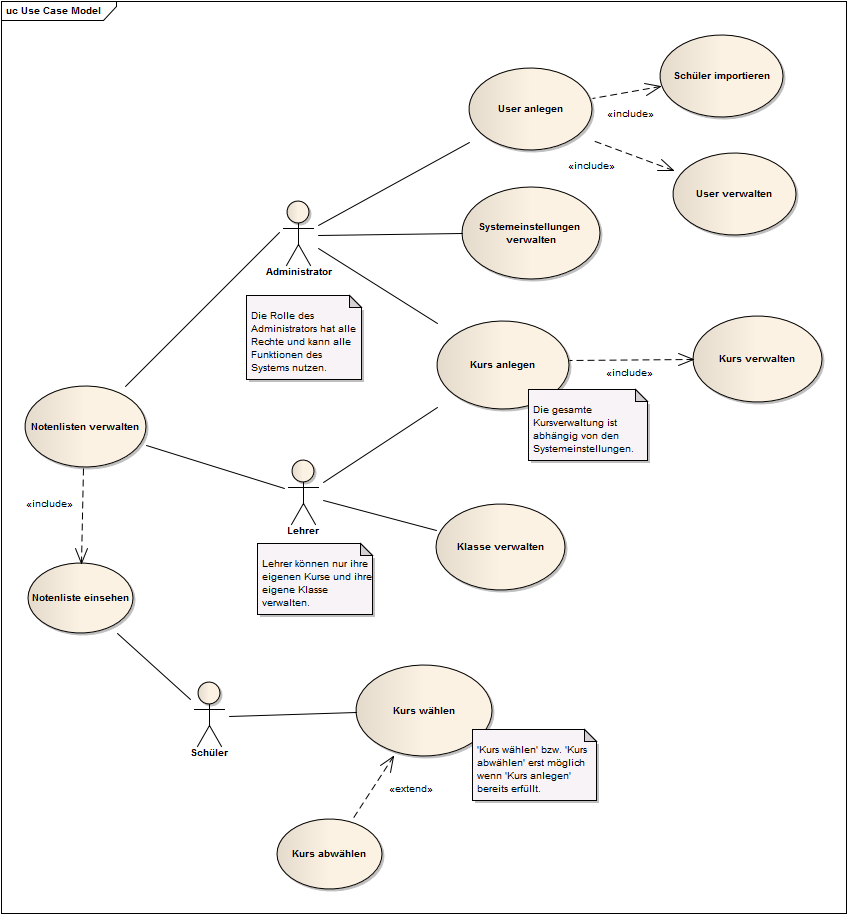
\includegraphics[scale=0.5]{img/UseCaseModel_kuwasys20.png}
 \end{center}
 \caption[\textbf{Use Case Diagram: Rollensystem}]{Use Case Diagramm: Rollensystem}
 \label{fig:UML_UC_kuwasys20}
\end{figure}

'Ein \ac{UC} beschreibt die Funktionalität des Softwaresystems, die ein Akteur ausführen muss, um ein gewünschtes Ergebnis zu erhalten oder um ein Ziel zu erreichen. \ac{UC}s sollen es ermöglichen, mit dem zukünftigen Benutzer über die Funktionalität des Softwaresystems zu sprechen, ohne sich gleich in Details zu verlieren.' Ein Zitat von \iz{Heide Balzert}{Informatikerin, die sich vor allem mit Fragen zum Thema Softwareengineering und -design beschäftigt. Derzeit ist sie Dozentin an der Fachhochschule Dortmund.}, entnommen aus \cite{BalzertH-UML2} auf Seite 28, welches den Sinn und Zweck eines \ac{UC-Diagramm}s präzise auf den Punkt bringt.

Zusammenfassend bedeutet dies, dass ein \ac{UC-Diagramm} immer dann sinnvoll ist wenn die Interaktionsmöglichkeit eines Systems, basierend auf verschiedene Aktueren, aufgezeigt werden soll. Die Akteure (dargestellt als 'Strichmännchen') im Diagramm, entsprechen genau denen, die später vom Rollensystem unterstützt werden sollen. Die Ellipsen zeigen die verschiedenen Anwendungsfälle die im System existieren. In einem so allgemeinen \ac{UC-Diagramm} wird absichtlich auf kleinste Details verzichtet. So bedeutet zum Beispiel der \ac{UC} 'Klasse verwalten' sowohl das Bearbeiten einer Klasse als auch das Vergeben von Noten oder andere klassenadministrative Aufwendungen.

Die gestrichelten Pfeile mit der Beschriftung '\texttt{$<<$include$>>$}' bezeichnen Anwendungsfälle in denen der \ac{UC}, auf welchen der Pfeil zeigt, implizit vorhanden ist wenn der \ac{UC}, von dem der Pfeil ausgeht, im System vorhanden ist. Das bedeutet wenn der \ac{UC} 'User anlegen' also vorhanden ist, auch die \ac{UC}s 'Schüler importieren' oder 'User verwalten' verwendet werden können. Ein erster \ac{UC} muss also immer erfolgen während ein zweiter (oder noch mehr) optional ausgeführt werden können.

Im Gegensatz hierzu bedeutet der gestrichelte Pfeil mit der Beschriftung '\texttt{$<<$extend$>>$}' von dem der Pfeil ausgeht, dass dieser \ac{UC} nur dann im System überhaupt vorhanden ist, wenn der \ac{UC} auf welchen der Pfeil zeigt im System vorhanden ist. Der \ac{UC} 'Kurs abwählen' ist also nur dann vorhanden wenn der \ac{UC} 'Kurs wählen' im System ausgeführt wurde. Der erste \ac{UC} wird durch den zweiten also erweitert.

\subsubsection{Statisches Analysemodell}

Im nächsten Schritt unserer Modellierung ist das statische Analysemodell, unter \prettyref{fig:UML_SA_kuwasys20} zu sehen, entworfen worden. Es stellt erste Überlegungen der Softwarearchitektur, mit konkreten Objekten inklusiver ihrer Attribute, dar und bildet ebenfalls die Beziehungen von Objekten zueinander ab. Genau genommen handelt es sich hierbei um ein 'abgespecktes' Klassendiagramm, in welchem die grobe Softwarestruktur erkennbar sein soll.

Die rechteckigen Formen stellen Klassen dar, die oben als Beschriftung ihren Namen tragen, unten die Attribute die zu ihr gehören. Die einfachen Linien sind Assoziationen zwischen den Klassen und können als Beziehungen interpretiert werden. Sie tragen einen Rollennamen und eine Multiplizität, um nachvollziehen zu können um wieviele Objekte einer Klasse es sich später mindestens und maximal handelt.
Die Rechtecke mit der Beschriftung \texttt{$<<$dataType$>>$ + String} stellen selbstdefinierte Datentypen dar.
Die Besonderheit in diesem Diagramm ist die Komposition (Assoziation mit einseitg schwarzer Raute). Sie sagt aus dass die Beziehung zwischen zwei Klassen einer starke Form der Aggregation entspricht. Die Teilklasse (Notenliste) kann also nur bestehen, solange die Aggregatklasse (Kurs) auch besteht. Würde, angewendet auf dieses Beispiel, ein Kurs gelöscht werden, würde auch der dazugehörige Notenlisteneintrag gelöscht werden. (Zur Vertiefung empfiehlt sich \cite{BalzertH_UML2} Seite 18)

In unserem Projekt entstanden zum Zeitpunkt des Softwareentwurfs 3 Klassen, die später für eine Interaktion mit dem System benötigt werden. Die Klasse für die Notenübersicht und für Kurse. Die verschiedenen Rollen wurden als Unterklassen der Klasse 'User' modelliert. Einzelne Datentypen, so bspw. für Daten zur Zeiterfassung (Datum) und zur Definition einzelner konstanter Strings (Name), wie die Rollen, wurden zur Vereinfachung vorgesehen.
Die Rollennamen sowie die Multiplizitäten der Assoziationen dürften selbsterklärend sein.

% Statisches Analyse Diagramm
\begin{figure}[H]
 \begin{center}
   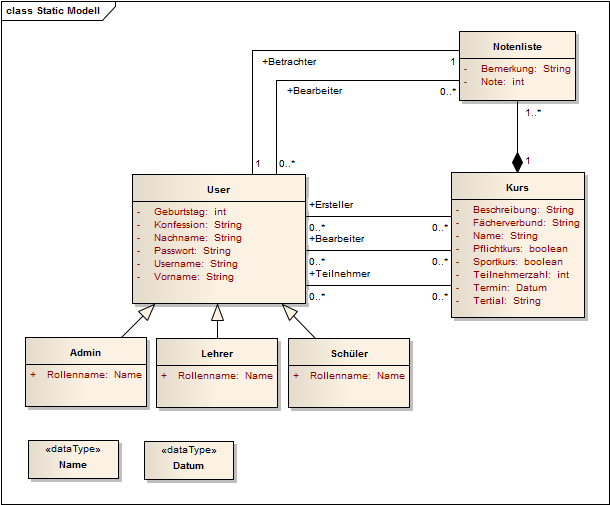
\includegraphics[scale=0.7]{img/StaticClassModel_kuwasys20.png}
 \end{center}
 \caption[\textbf{Statisches Analysemodell}]{Statisches Analysemodell}
 \label{fig:UML_SA_kuwasys20}
\end{figure}

\subsection{Benutzerschnittstellen und Rollensystem}\label{subsec:Benutzerschnittstellen und Rollensystem}

Das Kurswahlsystem der Schillerschule soll, laut Anforderungen, webbasiert mit Hilfe von verschiedenen Rollen konfiguriert und benutzt werden können.
Das System muss hierzu simultane Interaktionen, eines jeden Rollentyps, mit dem System zulassen. 

Per Aufgabendefinition liegen die vier Rollen, wie in \prettyref{subsec:Anforderungen an das System} bereits behandelt, zugrunde:

\begin{itemize}
  \item Schüler
  \item Kurslehrer
  \item Klassenlehrer
  \item Admin
\end{itemize}

Anhand der bereits vorgestellten \ac{OOM} sind, vor der Implementierung des Systems, die Rollenrechte und -richtlinien welche in den folgenden drei Unterabschnitten genaue beschrieben werden, modelliert worden.

\subsubsection{Die Rolle der Schüler}

Bei der Rolle der Schüler handelt es sich um die einfachste des Systems. 
Sie hat die wenigsten Rechte und kann hauptsächlich nur passiv, Ausnahme bildet hier die Kurswahl selbst, mit dem System interagieren.
Die Schüler welche das Kurswahlsystem erstmalig benutzen, befinden sich in der 7. Klasse. Jeder Schüler wird bis zum Abschluss der 9. Klasse das System benutzen.
Ein Schüler soll selbstständig seine Kurswahl für das jeweilige bevorstehende Tertial eines Schuljahres treffen können, dabei müssen bestimmte Abhängigkeiten eingehalten werden:

\begin{enumerate}
  \item 6 unterschiedliche Kurse pro Tertial
  \item 18 Kurse im Schuljahr
  \item 54 Kurse bis zur Vollendung des 9. Schuljahres
\end{enumerate}

\subsubsection{Die Rolle der Lehrer}

Der Rolle des Lehrers ist hingegen schon weitaus mehr Verantwortung auferlegt.
Das System unserer Webandwendung unterscheidet allerdings zwischen zwei verschiedenen Arten von Lehrern grundsätzlich nicht aufgrund einer Rollendefinition. 
Die Befugnis eines Lehrers sind lediglich abhängig von Werten die in der \ac{DB} gespeichert werden. 
Ein Klassenlehrer wird nur dann ein Klassenlehrer wenn für ihn eine Abhängigkeit zu einer Klasse besteht. 
Erst dann kann er die Funktionen, die einenm Klassenlehrer zu Verfügung stehen, nutzen.
Ein Klassenlehrer muss auf die ihm zugerordnete Klasse zugreifen und alle Kurse eines jeden Schülers einsehen können.

Das gleiche Prinzip gilt für Kurslehrer. 
Beim anlegen eines Kurses (eine Funktion die jedem Lehrer generell zur Verfügung steht) wird dieser Kurs dem Lehrer fest zugeordnet und wird somit zum Mitverantwortlichen der Kursverwaltung. 
Der Kurslehrer muss ebenfalls die Schüller einsehen können die sich in seinem Kurs befinden. Allerdings kann er nur ein Protokoll und eine Notenliste für Schüler in seinem Kurs führen.

In Abhängigkeit zur administrativen Systemverwaltung, auf die im nächsten Teil-Block eingegangen wird, hat der Lehrer nun die Rechte seine Kurse zu verwalten.

Zur Vereinfachung der Handhabung des Systems ist bereits an diesem Punkt der Modellierung an ein internes Protokollierungssystem gedacht worden. 
Es soll später die Kommunikation von Kurslehrern mit Klassenlehrern sowie die Kommunikation von Lehrern mit Schülern vereinfachen.
Im Rahmen unserer Projektarbeit wurde allerdings eine solche Funktionalität im System nicht implementiert.

\subsubsection{Die administrative Rolle des Systems}

Die administrativen Rechte des kompletten Systems stehen selbstverständlich nur dem Administrator zur Verfügung. Die Hauptaufgabe dieser Rolle im System ist es neue User ins System aufzunhemen und diese gegebenfalls zu Bearbeiten.
Das gilt für das Hinzufügen und Bearbeiten von Schülern und Lehrern gleichermaßen, beide Rollen haben also nicht die Möglichkeit sich selbst zu Verwalten.

Darüber hinaus verwaltet der Admin den Status des Systems, das aktuelle Schuljar und die dazughörigen Tertiale. Außerdem ist er der Hauptverantwortliche der Kursverwaltung.
Bevor ein Kurs stattfinden kann muss der Admin den Kurs aktivieren und für die Kurswahl zulassen. Eventuell müssen von ihm bestimmte Attribute eines Kurs noch angepasst werden können.
Ein Admin kann außerdem Fächerverbünde erstellen, bearbeiten und erstellte Kurse einem Fächerverbund zuordnen.

\subsubsection{Funktionalität des Systems}

Die Einteilung eines kompletten Schuljahrs geschieht jeweils in Tertiale. Dies kann grafisch in \prettyref{fig:Schuljahreinteilung} nachvollzogen werden. 

%%
% Schuljahreinteilung
\begin{figure}[h]
\begin{center}

\begin{tikzpicture}
    \node[draw=black, fill=yellow!20!] at (-2.5,5) {Unterteilung des Schuljahrs};
    \pie{33.3/Tertial 1, 33.3/Tertial 2, 33.3/Tertial 3}
\end{tikzpicture}

\end{center}
\caption[\textbf{Einteilung des Schuljahrs}]{Einteilung des Schuljahrs}
\label{fig:Schuljahreinteilung}
\end{figure}

Es war also nötig im administrativen Bereich des Systems eine Funktionalität vorzusehen, die es dem Admin ermöglicht das Schuljahr 'weiterzuschieben' und das entsprechende Tertial zu zu aktivieren.
Diese Verwaltungstätigkeit ist unumgänglich mit der Kurswahl verknüpft und muss für jede neu angepasst werden. 
Entscheidungen die hier während der Modellierung getroffen wurden, wurden im Hinblick auf eine möglichst einfaches \ac{UI} getroffen.

Jeder Kurs, der gewählt werden kann, gehört einem übergeordnetem Fächerverbund an, wie in \prettyref{fig:KursFaecherverbund} zu sehen ist.
Allerdings gibt es noch weitere Eigenschaften die Kurse erfüllen können. Ein Kurs kann ein Religionskurs sein, welcher für eine bestimmte Konfession ausgerichtet ist oder ein Sportkurs.
Ferner müssen Kurse als Pflichtkurse signifiziert werden können.
Aufgrund der Fülle an Informationen die verarbeitet werden müssen, war es in der Phase der Modellierung ebenfalls sehr wichtig die Datenstrukturen und deren Abhängigkeiten möglichst einfach zu halten, um in der späteren Implementierungsphase eine unkomplizierte Benutzerschnittstelle entwicklen zu können. 

%%
% Kurs - Fächerverbund
\begin{figure}[h]
\begin{center}

\begin{tikzpicture}
    \node[draw=black, fill=yellow!20!] at (-2.5,5) {Unterteilung des Schuljahrs};
    \pie{33.3/Tertial 1, 33.3/Tertial 2, 33.3/Tertial 3}
\end{tikzpicture}

\end{center}
\caption[\textbf{Einteilung des Schuljahrs}]{Einteilung des Schuljahrs}
\label{fig:KursFaecherverbund}
\end{figure}

%%
\todo[size=\small, color=green!40]{Grafik zur Abhängigkeit von Fächerverbünden bzw. Pflicht-/Sportkurse}
%%

Außer den beiden vorgestellten Datenverarbeitungen existieren selbstverständlich noch weitere, die vor allem im Sinne der Übersichtlichkeit des System  zum Tragen kommen. 
Dabei handelt es sich allerdings um Daten, die dynamisch während der Laufzeit erzeugt werden und deshalb ebenfalls in \prettyref{subsec:Systemrelevante Daten} genauer besprochen werden.
Im Gegensatz zu den dynamisch generierten Daten während der Laufzeit des Systems ist für alle anderen Daten zur Informationsverarbeitung eine Speicherung in einer Datenbank unabdingbar.
Im folgenden Unterabschnitt soll deshalb näher auf die Modellierung und Umsetzung des verwendeten Informationssystems eingegangen werden.

\subsection{Datenbankmodellierung}\label{subsec:Datenbankmodellierung}

Für die \ac{DB}-Modellierung wurde als erstes ein \ac{ER-Modell} skizziert, welches die Abhängigkeiten und Beziehungen zueinander verdeutlichen soll. Dieses ist in \prettyref{subsec:ERModell} abgebildet. Anschließend wurde das gesamte \ac{ER-Modell} in ein relationales Modell transformiert.
Mit dem entstandenen Relationalen Modell, welche in \prettyref{subsec:RelModell} dokumentiert ist, konnte anschließend auf dem Server die \ac{DB} inklusive der nötigen Tabellen erstellt werden.

\subsubsection{Entity-Relationship Modell}\label{subsec:ERModell}

Die \prettyref{fig:ERModell} zeigt das oben erwähnte \ac{ER-Modell} nach \iz{Peter Pin-Shan Chen}{Informatiker, der 1976 das ER-Modell entwickelte. Er gilt heute als Pioneer der \ac{OOM}.}, nachzulesen unter \cite{ChenPe} Seite 3 ff. bzw. \cite{VossenG-DDD} ab Seite 60.

\textbf{Aufbau des \ac{ER-Modell}s:}

Bei den blauen Rechtecken handelt es sich in diesem Modell um sogenannte Entities (Entity-Typen), die sind Dinge die in der \ac{DB} als solche abgebildet werden sollen. Sie stellen eine eigene Tabelle dar. Die gelben Ellipsen die diese umgeben, sind die Attribute (Attribut-Typen) der Entities, sie veranschaulichen die Daten welche Entities enthalten (können).
Die roten Rauten bezeichnen Beziehungen (Beziehungs-Typen) die zwischen Entities herrschen.

Das grüne Rechteck ist ein Spezialfall des 'Kurs'-Entities. Es wird als eigene Tabelle in der \ac{DB} dargestellt, ist im weitesten Sinne allerdings einer Aversion des 'Konfessions'-Attribut des 'Kurs'-Entities. Denkt man in diesem Fall an die \ac{UML}, so wäre an dieser Stelle wohl eine 'Enumeration' als eigener Datentype in Frage gekommen (Vrgl. \cite{BalzertH_UML2} Seite 10 und 11).

\tikzstyle{every entity} = [top color=white, bottom color=blue!30, draw=blue!50!black!100, drop shadow]
\tikzstyle{every weak entity} = [drop shadow={shadow xshift=.7ex, shadow yshift=-.7ex}]
\tikzstyle{every attribute} = [top color=white, bottom color=yellow!20, draw=yellow, node distance=1cm, drop shadow]
\tikzstyle{every relationship} = [top color=white, bottom color=red!20, draw=red!50!black!100, drop shadow]
\tikzstyle{every isa} = [top color=white, bottom color=green!20, draw=green!50!black!100, drop shadow]
\begin{center}
\begin{figure}[H]

\scalebox{.7}{
\begin{tikzpicture}[node distance=1.5cm, every edge/.style={link}]

%% USER
\node[entity] (usr) {Users};
\node[attribute] (usrvname) [above=2.5cm of usr] {VName} edge (usr);
\node[attribute] (usrnname) [above right=3cm of usr] {NName} edge (usr);
\node[attribute] (geb) [above left=3cm of usr] {Geburtsdatum} edge (usr);
\node[attribute] (usrkonf) [above left=of usr] {Konfession} edge (usr);
\node[attribute] (usrklasse) [above=of usr] {Klasse} edge (usr);
\node[attribute] (usrusername) [above right=of usr] {\key{Username}} edge (usr);
\node[attribute] (usrpassword) [right=of usr] {Passwort} edge (usr);
\node[attribute] (usrid) [below=0.3cm of usr] {\key{UserID}} edge (usr);

%% REL "hat"
\node[relationship] (hat) [left=1.5cm of usr] {hat} edge (usr);

%% REL "eingetragen"
\node[relationship] (eingetragen) [below left =3cm of usr] {eingetragen} edge (usr);
%
%% ROLLE
\node[entity] (rolle) [left=1cm of hat] {Rolle} edge (hat);
\node[attribute] (rollename) [left=of rolle] {\key{Username}} edge (rolle);
\node[attribute] (rolleusrnname) [above left=of rolle] {Rolle} edge (rolle);

%% REL "besucht"
\node[relationship] (besucht) [below right=of usr] {besucht} edge (usr);

%% KURS
\node[entity] (kurs) [below right=1cm of besucht] {Kurs} edge (besucht);
\node[entity, top color=white, bottom color=green!30, draw=green!50!black!100, drop shadow] (kurskonf) [above=1.5cm of kurs] {Kurskonfession} edge (kurs);
\node[attribute] (termin) [above right =.2cm of kurskonf] {Termin} edge (kurs);
\node[attribute] (kursl) [right =.2cm of kurskonf] {Kurslehrer} edge (kurs);
\node[attribute] (teilm) [above right=0.2cm of kurs] {Teilnehmerzahl} edge (kurs);
\node[attribute] (kursid) [left=0.2cm of kurs] {\key{KursID}} edge (kurs);
\node[attribute] (faecher) [right=0.2cm of kurs] {Fächerverbund} edge (kurs);
\node[attribute] (flags) [below=2.5cm of kurs] {Sportkurs} edge (kurs);
\node[attribute] (flag3) [below=2.2cm of faecher] {Pflicht} edge (kurs);
\node[attribute] (tertial) [below left=.2cm of flag3] {Tertial} edge (kurs);
\node[attribute] (flag2) [below=1.2cm of faecher] {Konfession} edge (kurs);
\node[attribute] (bemerk) [below=of kurs] {Beschreibung} edge (kurs);
\node[attribute] (kursname) [below right=0.2cm of kurs] {Kursname} edge (kurs);

%% REL "enthält"
\node[relationship] (enthalten) [below left =of kurs] {enthalten} edge (kurs);

%% NOTENLISTE
\node[entity] (notenliste) [below right=2cm of eingetragen] {Notenliste} edge (enthalten) edge (eingetragen);
\node[attribute] (note) [below left=1cm of notenliste] {Note} edge (notenliste);
\node[attribute] (usrkonf) [above =of notenliste] {Bemerkung} edge (notenliste);
\node[attribute] (usrvname) [below=of notenliste] {\key{KursID}} edge (notenliste);
\node[attribute] (usrnname) [left=of notenliste] {\key{UserID}} edge (notenliste);
\node[attribute] (listid) [below right=1.2cm of notenliste] {\key{ListenID}} edge (notenliste);

%% SYSTEM
\node[entity] (system) [below=5cm of notenliste] {System};
\node[attribute] (schuljahr) [below=of system] {Schuljahr} edge (system);
\node[attribute] (tertial) [left=of system] {Tertial} edge (system);
\node[attribute] (wochd) [below left= of system] {Phase} edge (system);
\end{tikzpicture}
}
\caption[\textbf{Entity-Relationship Modell}]{Entity-Relationship Modell}
\label{fig:ERModell}
\end{figure}
\end{center}

\textbf{Interpretation des \ac{ER-Modell}s:}

Um die Interpretation, also den Gedankengang der \ac{DB}-Modellierung, zu verdeutlichen macht es Sinn, die Beziehungen genau auszuformulieren.
Dabei werden alle Beziehungen zu jedem Entity betrachtet, begonnen mit dem Entity.
Zusätzlich sollen die Multiplizitäten mit einfließen, um die Abhängigkeiten zu verdeutlichen und um die Transformation in ein Datenbankmodell zu erleichtern.

Die Schreibweise dieser Multiplizitäten ist wie folgt definiert:

Sei $E_{A}$ das erste und $E_{B}$ das zweite Entity.
Die Beziehung beider Entities ist definiert als $R_{AB}$. 
Die erste Multipliziät $(0,N)$ gibt Auskunft über die Häufigkeit von $E_{A}$ in der geltenden Beziehung zu $E_{B}$.
Die zweite $(1;M)$ über die Häufigkeit von $E_{B}$ zu $E_{A}$.

Man kann also schreiben:

\begin{center}
$E_{A}$ ist $(0;N)$ in Beziehung $R_{AB}$ zu $E_{B}$

oder

$E_{B}$ ist $(1;M)$ in Beziehung $R_{AB}$ zu $E_{A}$
\end{center}

Wobei die erste Zahl bei der Angabe der Multiplizität, also die vor dem Semikolon (';') für die minimalste, die zweite Zahl für die maximalste Gültigkeit unter der bestendenen Bedingung steht.

Begonnen werden soll die genauere Betrachtungsweise mit dem Entity 'User':

\begin{enumerate}
  \item User - Rolle (beidseitig):	
    \begin{itemize}
      \item einem User ist genau $(1;1)$ Rolle zugeteilt
      \item einer Rolle hingegen können $(0;N)$ User zugeteilt sein
    \end{itemize}

  \item User - Kurs
    \begin{itemize}
      \item ein Schüler wählt $(0;N)$ viele Kurse
      \item ein Lehrer erstellt/verwaltet $(0;M)$ viele Kurse
    \end{itemize}
  
  \item User - Notenliste:
    \begin{itemize}
      \item ein Schüler hat $(1;1)$ Eintrag in der Notenliste für jeweils einen fest zugeordneten Kurs (Vrgl. Kurs - Notenliste)
    \end{itemize}

\end{enumerate}

Konkretisieren wir nun das Entity 'Kurs':

\begin{enumerate}
  \item Kurs - Notenliste:
  \begin{itemize}
    \item ein Kurs besitzt genau $(1;1)$ Eintrag pro Kurs in der Notenliste für einen Schüler (Vrgl. User - Notenliste)
  \end{itemize}
  
  \item Kurs - Kurskonfession	
    \begin{itemize}
      \item ein Kurs hat genau $(0;1)$ Konfessionszugehörigkeit
    \end{itemize}

  \item Kurs - User	
    \begin{itemize}
      \item ein Kurs wird von $(0;N)$ vielen Schülern gewählt
      \item ein Kurs wird immer genau $(1;1)$ Lehrern zugeteilt
    \end{itemize}
\end{enumerate}

Für das letzte Entity der Dreier-Beziehung 'Notenliste' gelten lediglich die bereits beschriebenen Abhängigkeiten und Beziehungsverhältnisse. 
Zur Verdeutlichung sollen diese jedoch nochmals aufgeführt werden.

\begin{enumerate}
  \item Notenliste - User:
  \begin{itemize}
    \item eine Notenliste hat im Bezug auf genau einen Kurs $(0;N)$ Einträge für einen User
  \end{itemize}
  
  \item Notenliste - Kurs:
  \begin{itemize}
    \item Ein Schüler wählt $(1;N)$ viele Kurse, ein Kurs wird von $(1;N)$ vielen Schülern besucht/gewählt.
  \end{itemize}
  
\end{enumerate}

Das Entity 'System' besitzt keine Beziehungen innerhalb der Datenbank, weshalb auf eine ausführliche Interpretation verzichtet werden kann.
Die Darstellung dieses Entities wird innerhalb der \ac{DB} sowieso über eine eigene Tabelle umgesetzt.

Der nächste Schritt ist nun die Transformation von \ac{ER-Modell} in das Relationale \ac{DB}-Modell.

\subsubsection{Relationales Modell}\label{subsec:RelModell}

Bei der Beschreibung des Relationalen Modells der KuWaSys-\ac{DB} ist das Hauptaugenmerk auf die komplette Datenverarbeitung gelegt, also vor allem auch Implementierungen für Vorgänge die für den Benutzer des Systems nicht unmittelbar zu sehen sind.
Daten die für die Oberfläche und die einzelnen Benutzerschnittstellen eine tragende Rolle spielen sollen unter (Abschnitt Benutzerschnittstellen) gesondert behandelt werden und werden im Laufe dieses Kapitels nur kurz angesprochen.

Die Vorüberlegungen zur Transformation von mehrwertigen Attributen von Entities sind bereits abgeschlossen.
Prinzipiell kann man mit der Transformation, wie in \cite{VossenG-DDD} beschrieben ist wie folgt vorgehen:

\begin{enumerate}
 \item Jedes Entity wird in eine relationale Form gebracht
 \item Jeder Beziehungs-Typ ebenfalls, es sei denn:
 \begin{itemize}
  \item es handelt sich um eine zweistellige $1:1$-Beziehung
  \item es handelt sich hierbei um eine $1:N$-Beziehung
 \end{itemize}
\end{enumerate}

Die Beschreibung $1:1$- bzw $1:N$-Beziehung bedeutet in diesem Fall allerdings nicht wie zuvor, ein Minimum auf der linken und das Maximum auf der rechten Seite. 
Hierbei werden nur noch die maximalen Werte der beiden Multiplizitätsangaben berücksichtigt. Dies gilt analog für alle Angaben der Multiplizitäten.

Sollte bei der Transformation $Punkt$ $2)$ eine Rolle spielen, müssen Attribute in bereits bestehende Relationsschemata aufgenommen werden. Folgende Regeln treten dann in Kraft:
\begin{enumerate}
 \item Zweistellige $1:1$-Beziehung
 \begin{itemize}
  \item ein Entity stellt selbst ein Relationsschema dar
  \item Attribute des zweiten Entities werden ebenfalls in dieselbe Tabelle gespeichert
 \end{itemize}
 \item Zweistellige $1:N$-Beziehung
 \begin{itemize}
  \item ein Entity stellt ein eigenes Relationsschema dar
  \item erste Möglichkeit: die Attribute des Entities welches die maximale Multiplizität von $1$ aufweist wird hingegen dem Realtionsschema mit der maximalen Multiplizität von $N$ in Form von Fremdschlüsseln zugeschrieben
  \item zweite Möglichkeit: es wird ein eigenes Relationsschema für die Beziehung der beiden Entities angelegt. Dieses neu entstande Schema erhält dann Attribute, welche widerum Fremdschlüssel der beiden anderen Entities sind
 \end{itemize}
\end{enumerate}

Die Transformation vom \ac{ER-Modell} ins Relationale Modell (zur bildhaften Darstellung ist die Kopfzeile der dazugehörigen Tabelle auch gezeigt) sieht im Falle des Kurswahlsystems folgendermaßen aus:

\textbf{Users} = \{( \underline{id:serial}, nachname:character, vorname:character, geburtstag:character, konfession:character, klasse:character, \underline{username:character}, passwort:character )\}

% User-Tabelle
\begin{table}[H]
\begin{center}
	\begin{tabular}{|c|c|c|c|c|c|c|c|}\hline
		\textbf{\underline{ID}} & \textbf{NName} & \textbf{VName} & \textbf{Geb} & \textbf{Konf} & \textbf{Klasse} & \textbf{\underline{Username}} & \textbf{Passwort} \\ \hline
		\vdots & \vdots & \vdots & \vdots & \vdots & \vdots & \vdots & \vdots \\
	\end{tabular}
	\caption{Kopfzeile der User-Tabelle}
\end{center}
\end{table}

\textbf{Kurs} = \{( \underline{id:serial}, name:character, kurslehrer:integer, faecherverbund:character, termin:integer, beschreibung:character, schuljahr:integer, tertial:integer, 
teilnehmerzahl:integer, pflichtkurs:boolean, sport:boolean )\}

% Kurs-Tabelle
\begin{table}[H]
\begin{center}
	\begin{tabular}{|c|c|c|c|c|c}\hline
		\textbf{\underline{ID}} & \textbf{Name} & \textbf{Kurslehrer} & \textbf{Faecherverbund} & \textbf{Termin} & \dots \\ \hline
		\vdots & \vdots & \vdots & \vdots & \vdots & \dots \\
	\end{tabular}
	\caption{Kopfzeile der Kurs-Tabelle  (unvollständig)}
\end{center}
\end{table}

\textbf{Kurs-Konfessionen} = \{( \underline{religionid:integer}, konfession:character )\} 
 
% Kurs-Konfession-Tabelle
\begin{table}[H]
\begin{center}
	\begin{tabular}{|c|c|}\hline
		\textbf{\underline{ReligionID}} & \textbf{Konfession} \\ \hline
		\vdots & \vdots \\
	\end{tabular}
	\caption{Kopfzeile der Kurs-Konfessions-Tabelle}
\end{center}
\end{table}

\textbf{Notenliste} = \{( \underline{id:serial}, note:integer, bemerkung:character, userid:integer, kursid:integer, jahr:integer, tertial:integer )\}

% Notenliste-Tabelle
\begin{table}[H]
\begin{center}
	\begin{tabular}{|c|c|c|c|c|c|c|}\hline
		\textbf{\underline{ID}} & \textbf{Note} & \textbf{Bemerkung} & \textbf{UserID} & \textbf{KursID} & \textbf{Jahr} & \textbf{Tertial}\\ \hline
		\vdots & \vdots & \vdots & \vdots & \vdots & \vdots & \vdots  \\
	\end{tabular}
	\caption{Kopfzeile der Notenlisten-Tabelle}
\end{center}
\end{table}

\textbf{Rolle} = \{( \underline{username:character}, rolle:character )\}

% Rollen-Tabelle
\begin{table}[H]
\begin{center}
	\begin{tabular}{|c|c|}\hline
		\textbf{\underline{Username}} & \textbf{Rolle} \\ \hline
		\vdots & \vdots \\
	\end{tabular}
	\caption{Kopfzeile der Rollen-Tabelle}
\end{center}
\end{table}

\textbf{System} = \{( \underline{phase:integer}, jahr:integer, tertial:integer )\}

% System-Tabelle
\begin{table}[H]
\begin{center}
	\begin{tabular}{|c|c|c|}\hline
		\textbf{\underline{Phase}} & \textbf{Jahr} & \textbf{Tertial} \\ \hline
		\vdots & \vdots & \vdots \\
	\end{tabular}
	\caption{Kopfzeile der System-Tabelle}
\end{center}
\end{table}

\subsection{Konfiguration der Laufzeitumgebung und des Servers}\label{subsec:Konfiguration der Laufzeitumgebung und des Server}

Dieses Kapitel ist als Zwischenschritt, von der Modellierung zur Implementierung, unseres Softwareprojekts zu verstehen.
Zum Einen galt es eine komplette bestehende Infrastruktur zu überblicken und zu verstehen (dieser Schritt kann als eine Art der Modellierung verstanden werden)
zum Anderen musste ein komplettes neues System einwandfrei funktionsfähig eingebettet werden (zu vergleichen mit dem Schritt der Implementierung).

\textbf{Sichtung der bestehenden Infrastruktur:}

Die Schillerschule teilt sich mit der benachbarten Realschule am Galgenberg eine Serverinfrastruktur nach der Novell Musterlösung paedML 3.33, weitere Informationen sind unter \cite{paedML} zu finden. % VMWare ASG 220 Astaro.
Diese beinhaltet eine virtuelle Infrastruktur \gls{VMWare} ESXi auf der ein \ac{SLES} Novell Server gehostet ist.

\begin{figure}[H]
\begin{center}
\begin{tikzpicture}[
  scale=0.1,
  font=\sffamily,
  every matrix/.style={ampersand replacement=\&,column sep=2cm,row sep=2cm},
  source/.style={draw,thick,rounded corners,fill=yellow!20,inner sep=.3cm},
  process/.style={draw,thick,circle,fill=blue!20},
  sink/.style={source,fill=green!20},
  datastore/.style={draw,very thick,shape=datastore,inner sep=.3cm},
  dots/.style={gray,scale=2},
  to/.style={->,>=stealth',shorten >=1pt,semithick,font=\sffamily\footnotesize},
  every node/.style={align=center}]

  % Positionierung über Matrix-Layout
  \matrix{

    \node[source] (Ubuntu) {Ubuntu 12.04 VM\\ ($141.10.50.250$)};
      \& \node[process] (Suse) {Server}; \& \\
      \& \node[sink] (firewall) {ASG 220 Astaro\\ ($Firewall$)}; \& \\

    \node[source] (SLES) {SuSE Linux\\ Enterprise Server\\ ($SLES$)}; \& \\

    \node[datastore, color=black!50!white] (infrastructure) {Einstellungen\\($Novell$ $paedML$ $3.3$)}; \& \\


      \& \node[process] (router) {Router};
      \& \node[sink] (www) {WWW}; \\
  };

  % VM - Host
  \draw[to, very thick] (Ubuntu) -- node[midway,above] {VM Host}
      node[midway,below] {} (Suse);

  % FW - Host
  \draw[to, dashed, very  thick] (Suse) -- node[midway,above] {}
       node[midway,below] {} (firewall);itemize
  \draw[to, dashed, very  thick] (firewall) -- node[midway,above] {}
       node[midway,below] {} (Suse);

  % FW - Router
  \draw[to, very thick] (router) -- node[midway,above] {}
       node[midway,below] {} (firewall);
  \draw[to, very  thick] (firewall) -- node[midway,above] {}
       node[midway,below] {} (router);

  % Einstellungen Infrastruktur
  \draw[color=black!50!white] (infrastructure) -- node[midway,above] {}
       node[midway,below] {} (SLES);

  % SLES - Netz
  \draw[to, very thick] (SLES) -- node[midway,above=1cm] {VM Host}
       node[midway,below] {} (Suse);
  \draw[to, dashed, color=black!50!white] (SLES) -- node[midway,right=0.2cm] {Konfiguration}
       node[midway,below] {} (router);
  \draw[to, dashed, color=black!50!white] (SLES) -- node[midway,right=0.2cm] {Konfiguation}
       node[midway,below] {} (Ubuntu);

  % Router - WWW
  \draw[to, very thick] (router) -- node[midway,above] {}
       node[midway,below] {} (www);
  \draw[to, very thick] (www) -- node[midway,above] {}
       node[midway,below] {} (router);
\end{tikzpicture}
\end{center}
\caption[\textbf{Netzwerkstruktur der Schillerschule Aalen}]{Netzwerkstruktur der Schillerschule Aalen mit DMZ}
\label{fig:Netzwerkstruktur}
\end{figure}

Prinzipiell wäre eine Verwendung dieser virtuellen \gls{Appliance} zum Hosting der \ac{Webapp} möglich. Um jedoch die Systemsicherheit zu erhöhen ist eine weitere virtuelle Appliance, die nur das Kurswahlsystem bereitstellt die bessere Wahl.
\iz{Ubuntu Server 12.04 LTS}{http://www.ubuntu.com/} läuft auf diesem virtuellen Rechner, der sich wie der oben genannte SLES in der \gls{DMZ} der virtuellen Netzwerkinfrastruktur befindet.

\textbf{Integration in die Infrastruktur:}

Ein PostreSQL-Server dient zur Datenhaltung und ein Apache Tomcat 7 zur Auslieferung der \ac{Webapp}. Nach Konfiguation (und überfälligem reboot) der Astaro Firewall im Keller der Schule ist die Webapp jetzt über das Intranet an allen Rechnern im Schulnetz erreichbar (\url{http://192.168.1.222:8080/kuwasys20}). Die Erreichbarkeit über das Internet ist seit der Freischaltung der entsprechenden Ports auf den BelWü-Server und umgekehrt gegeben (\url{http://141.10.50.250:8080/kuwasys20}).
Diese Adressen werden auf der Homepage der Schillerschule und im Intranet verlinkt, sodass keine weitere Maskierung wie Subdomains oder lokale DNS-Einträge notwendig ist.
Die Admnistration des Ubuntu Servers kann im Intranet von einer VMWare Management Console aus erfolgen, für schnelles Eingreifen wurde ein \gls{Secure Shell} (SSH) Zugang eingerichtet, der im Internet erreichbar ist.

In \prettyref{fig:Netzwerkstruktur} ist die neue Struktur des Netzwerks dargestellt.

Die Einrichtung eines Backups war für unser Projekt nicht notwendig, da die Schillerschule selbst schon über ein funktionsfähiges Backupsystem verfügt. Hierbei wird in bestimmten Intervallen die komplette Festplatte des Servers gespiegelt, und somit auch die virtuellen Maschinen.
Somit ist die Garantie gegeben, dass auch das Kurswahlsystem einem ständigen Sicherungsvorgang unterliegt und im Notfall wiederhergestellt werden kann.
\newpage

\section{Implementierung}	\label{sec:Implementierung}
							\label{secmin:Implementierung}

In einem System, in welchem ein \gls{Multi-User Betrieb} möglich sein soll, ist das Design der Oberfläche und das der einzelnen Benutzerschnittstellen unweigerlich eng miteinander verknüpft. 
Es müssen in der Phase der Implementierung bereits exakte Schnittstellen definiert und strukturierte Oberflächen skizziert worden sein um spätere Korrekturen gering zu halten oder um sie zu vermeiden.

In den folgenden zwei Abschnitten sollen grundlegende Implementierungsgedanken besprochen werden, die mit den Anforderungen an das System in erster Linie nichts zu tun haben. 
Zuerst soll die Art und Weise der Umsetzung der Benutzerschnittstellen und des Designs näher erklärt werden. Danach sollen elementare Datenstrukturen die zum Einsatz kamen und in JSF implementiert wurde näher erläutert werden.

Nach den beiden einführenden Abschnitten wird dem Leser detailiert dargestellt wie die zu bewältigenden Systemanforderungen in JSF umgesetzt wurden. 
Dabei werden Quellcodeausschnitte sowie Diagramme zum Einsatz kommen die dem Leser das Verstehen erleichtern sollen.
Da während allen Phasen der Umsetzung des Projekts auch immer die Modularität des gesamten Systems im Vordergrund stand soll hier nicht kleinlichst genau erklärt werden was im Quellcode steht, sondern darauf eingegangen werden, wie das zu lösende Problem angegangen wurde und schlussendlich welche wichtigen Bausteine zu tragen kamen. 
An dieser Stelle soll außerdem nochmals die Wichtigkeit der oben besprochenen Datenbankmodellierung erwähnt werden. Gründe für die verschiedenen Umsetzungen der Modellierung sollen im Abschnitt der Implementierung dieser Ausarbeitung nicht mehr näher besprochen werden. 
Es wurde jedoch viel Wert darauf gelegt die Schritte der Implementierung gut und verständlich zu formulieren und darzustellen.

\subsection{Benutzerschnittstellen und Oberflächendesign}

Wir haben uns für ein simples und einfach zu verstehendes Oberflächendesign entschieden, welches allerdings den Design Aspekten der \gls{Corporate Identity} (CI) erfüllen sollte. 
%%
\todo[size=\small, color=green!40]{HMI Buch Zitate etc...}
%%
Im allgemeinen wird beim Screendesign bestimmten Regeln gefolgt, welche durch das gewählte Gestaltungsraster festgelegt werden.

Hierzu wurden von uns folgende Bereiche festgelegt:
\begin{itemize}
  \item Kopf- oder Bannerbereich mit Logo
  \item Navigationsbereich bzw. Unternavigation
  \item Arbeitsbereich
  \item Impressum/Hinweise
\end{itemize}

Der Hauptaufbau dieser Seiten, auf welche im folgenden näher eingegangen wird, wurden mit Templates, wie es bereits in \prettyref{subsec:Darstellung von Seiteninhalten} angesprochen wurde, umgesetzt.
Der allgemeine Aufbau soll im folgenden besprochen werden, der nachstehende Quellcodeausschnitt zeigt einen Teil des Templates das von uns zur Gestaltung der Seiten verwendet wurde:

% LISTING
% template.xhtml 
%%
\todo[size=\small, color=red!40]{Listing}
%%
Auffallend ist vor allem der Kopf der Seite, welcher den Wiedererkennungswert (Vrgl. hierzu die \iz{Webiste der Schillerschule}{\url{http://www.schillerschule-aalen.de}}) ganu im Sinne des \ac{CI}s steigern soll.
Hierzu wurde die Grafik lediglich transparenter gehalten als ihr Original und hat ganz im Stil der Schule die Überschrift erhalten wie in \prettyref{fig:header_KuWaSys} zu sehen ist.

% Header
\begin{figure}[H]
 \begin{center}
   
\includegraphics[scale=0.4]{img/header_KuWaSys.png}
 \end{center}
 \caption[\textbf{KuWaSys: Banner des Systems (Header)}]{KuWaSys: Banner des Systems (Header)}
 \label{fig:header_KuWaSys}
\end{figure}

Die Navigation und deren Unternavigationspunkte sind im linken Bereich der Webiste angeordnet und unterstützen den User visuell mit Hervorhebungen, wie in \prettyref{fig:navihervorhebung_KuWaSys} dargestellt ist, bei der Arbeit mit dem System.
Nötige Unternavigationspunkte, falls diese vorhanden sind, öffnen sich automatisch beim Klick auf ein übergeordnetes Menüelement, sodass die komplette Menüstruktur handlich und kompakt dargestellt erscheint und mit einem Blick erfasst werden kann.

Der Arbeitsbereich wird in der Mitte der Seite dargestellt, unterhalb des Kopfbereichs und rechts der Navigation. 
Dieser wird abgetrennt durch blaue Balken (links zur Navigation sowie oben zum Kopfbereich) um die Einteilung der Seite für die Benutzer des Systems eindeutig und übersichtlich zu halten.
Jede Interaktion mit dem System wird in diesem Bereich der Website dargestellt. 
%%
\todo[size=\small, color=green!40]{Grafik zu Bildschirmenteilung}
%%

% Infobar
\begin{figure}[h]
 \begin{center}
   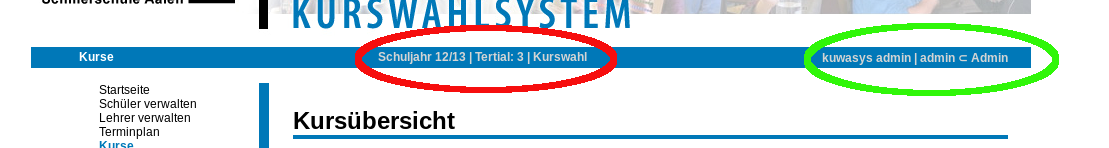
\includegraphics[scale=0.4]{img/informationbar_KuWaSys.png}
 \end{center}
 \caption[\textbf{KuWaSys: Informationsbalken (oberer Bereich)}]{KuWaSys: Informationsbalken (oberer Bereich)}
 \label{fig:infobar_KuWaSys}
\end{figure}

Zur erwähnen ist zudem noch der Trennbalken nach oben welcher zusätzlich als Informationsanzeige für den User verwendet wird und der Fußbereich welcher Informationen zur Website enthält. 
Die obere Anzeige, hier werden Informationen zum User selbst (Voller Name, Username und Rolle im System) und Informationen zum aktuellen Status des Systems (aktuelles Schuljahr und aktuelles Tertial) angezeigt.
Die \prettyref{fig:infobar_KuWaSys} zeigt die genaue Einteilung des Infobalkens oben, rot die Informationen des Systems, grün die Informationen des Users.
Der Fußbereich dient ausschließlich zur weiteren Information beim Besuch der Webiste welcher in \prettyref{fig:footer_KuWaSys} zu sehen ist.  

Die Hauptfarben des Systems wurden absichtlich blau gewählt um eine gewisse Professionalität sowie Seriösität gegenüber den Benutzern auszustrahlen. Diese ziehen sich kontinuierlich durch das gesamte System

%%
\todo[size=\small, color=green!40]{HMI Buch Dahm...}
%%

% Navibar
\begin{wrapfigure}[18]{r}{12cm}
 \begin{center}
   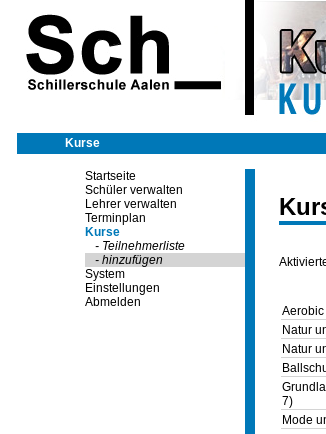
\includegraphics[scale=0.65]{img/navigation_KuWaSys.png}
 \end{center}
 \caption[\textbf{KuWaSys: Navigations und Menüelemente (linker Bereich)}]{KuWaSys: Navigations und Menüelemente (linker Bereich)}
 \label{fig:navihervorhebung_KuWaSys}
\end{wrapfigure}

Auf ein Impressum oder auf rechtliche Hinweise konnte bei dieser Art von Webiste verzichtet werden. 
Erstens handelt es sich hierbei um keine kommerzielle Website, laut \textit{§5} \ac{TMG} wird ein Impressum von 'geschäftsmäßigen Online-Diensten' benötigt, 
%%
\todo[size=\small, color=green!40]{rechtlicher Nachweis} zweitens um keine öffentliche oder frei zugängliche Website, 
%%
wobei hier die Vorschrift des \textit{§55} \ac{RstV} besagt, dass eine Impressumspflicht nur dann besteht wenn der Inhalt der Website regelmäßig journalistisch-redaktionelle Inhalte online zur Verfügung stellt.
(Gesetzesauszüge sind im Anhang unter \prettyref{subsec:Gesetz} zu finden) 

% Footer
\begin{figure}[h]
 \begin{center}
   
\includegraphics[scale=0.7]{img/footer_KuWaSys.png}
 \end{center}
 \caption[\textbf{KuWaSys: Informationsbalken (unterer Bereich)}]{KuWaSys: Informationsbalken (unterer Bereich)}
 \label{fig:footer_KuWaSys}
\end{figure}

Zur Strukturierung von Seiteninhalten wurden herkömmliche \ac{JSF}-Standardkomponenten verwendet.
Zu den hauptsächlich verwendeten, zählen:
\begin{itemize}
  \item \texttt{<h:outputText>}\\
    Element welches HTML-Text auf der Obefläche ausgibt 
  
  \item \texttt{<h:outputLabel>}\\
    auch normaler Text, allerdings als Beschriftung von Texteingabefeldern
      
  \item \texttt{<h:inputText>}\\
    Element zur Texteingabe, Synonyme für ein HTML \texttt{<input>}-Tag mit type="text"
  
  \item \texttt{<h:inputSecret>}\\
    Element zur verschlüsselten Texteingabe, entspricht \texttt{<input>}-Tag mit type="password"
  
  \item \texttt{<h:commandButton>}\\
    Button in HTML, der Klick löst eine definierte Aktion über eine ManagedBean-Methode aus

  \item \texttt{<h:panelGrid>}\\
    Darstellung einer Tabelle, Synonym für das HTML \texttt{<table>}-Tag. Die Anzahl der Spalten wird über das \texttt{columns}-Attribut festgelegt
  
  \item \texttt{<h:panelGroup>}\\
    Container-Element (mehrere JSF-Tags werden zu einem zusammenfügt)
  
  \item \texttt{<h:message>}\\
    gibt eine Fehlermeldung für die definierte Komponenten aus (\texttt{ErrorStyle}-Attribut über \ac{CSS} steuerbar)
  
  \item \texttt{<h:form>}\\
    stellt ein Formular dar, welches einen POST-Request per HTTP absetzt
  
  \item \texttt{<f:facet>}\\
    Definiert eine Facette (bspw. die Überschrift für eine Tabelle)
\end{itemize}

Außer den eben erwähnten Komponenten gibt es eine Vielzahl anderer bis hin zu selbstdefinierten welche im entwickelten System zum Einsatz kommen. Diese werden allerdings nicht näher betrachtet, da sie für das umgesetzte System irrelevant sind. Selbstverständlich kann zur grafischen Darstellung auch normale \ac{HTML}-Syntax verwendet werden.
Um die Strukturierung des Seitenaufbaus übersichtlich zu halten wird ebenfalls das wohl bereits bekannte Grundlagenwerkezug der Webentwicklung, die \gls{Cascading Style Sheets} (CSS), für die Eigenschaften der Darstellungselemente, eingesetzt.
Vorteile dieser Vorgehensweise der Datenverarbeitung resultiert in einer einheitlichen und damit gut strukturierten Darstellung der betroffenen Websites.

%%
\todo[size=\small, color=green!40]{CSS/Komponenten Listings}
%%

\subsection{Informationsdarstellung und -verarbeitung}

Eine elementare Datenstrukturen im System sind Listen, welche dem User in Form einer Tabelle dargestellt werden.
Die Vorteile dieser Datenstruktur sind die Einfachheit der Datenhaltung sowie der Zugriff auf die Daten und Bereitstellung dieser.

Grundlegend sind zwei zu unterscheidende Listen im System implementiert:
\begin{enumerate}
  \item User-Listen (Schüler und Lehrer)
  \item Kurs-Listen
  \item Noten-Listen
\end{enumerate}

Dabei sind beide Listen lediglich nach Art des Inhalts ihrer Daten zu differenzieren. Die für die Benutzeroberfläche relevanten sollen kurz erläutert werden:

\textbf{Schüler}
\begin{itemize}
  \item ID: Integer, welcher für das Wählen von Kursen und das Vergeben von Noten wichtig ist, da diese einen Fremdschlüssel in der jeweiligen Tabelle darstellt
  \item Vorname und Nachname: String, der den realen Namen des Users wiedergibt
  \item Klasse: String, zur Identifizierung welchem Klassenlehrer ein Schüler zugeordnet ist, bzw wie weit er in seiner Schullaufbahn vorangeschritten ist
  \item Konfession: String, zur Identifizierung des Religionsunterrichts der angeboten werden kann bzw. muss während dem Erstellen eines Kurses. (Näheres in Abschnitt Kurswahl)
\end{itemize}

\textbf{Lehrer}
\begin{itemize}
  \item ID (mit der gleichen Bedeutung wie bei Schülern)
  \item Vorname und Nachname (ebenfalls gleich wie bei Schülern)
  \item Klasse: String, der festlegt, von welcher Klasse ein Lehrer Klassenlehrer ist
\end{itemize}

\textbf{Kurse}
\begin{itemize}
  \item Kursnummer
  \item Kursname
  \item Kursbeschreibung
  \item Teilnehmeranzahl
\end{itemize}

\textbf{Notenlisten}
\begin{itemize}
  \item Schülername
  \item Kursname
  \item Note
  \item Bemerkung
\end{itemize}

Die Implementierung der Listen in Java wurde über Listen vom Typ \texttt{ArrayList<List>} umgesetzt. 
%%
\todo[size=\small, color=orange!40]{technische Umsetzung von Listen, Grundlagen etc... am Beispiel von Java Listings - 1 bis 2 Getter/Setter}
%%
%%
\todo[size=\small, color=orange!40]{dazugehöriges Facelet, bpw. Schüler}
%%
%%
\todo[size=\small, color=orange!40]{Datenbankabfrage und 'Befüllen' der Listen}
%%


\subsection{Benutzerauthentifizierung}

Einer der elementarsten Vorgänge im System ist der Login-Vorgang. Es handelt sich hierbei um einen Vorgang den jeder Benutzer egal mit welcher Rolle vor der Interkation mit dem System durchlaufen muss. Zur Verifizierung eines Users am System wird sein Kürzel, welches beim Anlegen automatisch aus Vor- und Nachnamen generiert wird, sowie ein Passwort, welches ebenfalls automatisch und randomisiert generiert wird, benötigt. Die Anmeldemaske, welche zugleich auch die Startseite des Kurswahlsystems bildet, kann in \prettyref{fig:login_KuWaSys} angesehen werden. Die Registrierung eines Users am System kann ausschließlich durch den Admin erfolgen.

% Login
\begin{wrapfigure}[12]{l}{10cm}
 \begin{center}
   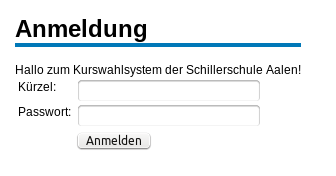
\includegraphics[scale=0.7]{img/login_KuWaSys.png}
 \end{center}
 \caption[\textbf{KuWaSys: Login Maske und Startseite}]{KuWaSys: Login Maske und Startseite}
 \label{fig:login_KuWaSys}
\end{wrapfigure}


Für den Vorgang des Logins am System besitzt der Servlet-Container Tomcat 7 eine sehr hilfreiche und gängige Funktion der Softwareentwicklung, die Konfiguation des \ac{DBCP}s des Apache Commons Projekts. Nähere Informationen sind unter \cite{ApacheDBCP} zu finden. 

Wie bereits aus dem \prettyref{subsec:Datenbankmodellierung} bekannt ist, haben wir für unser Datenbank eine zusätzliche Tabelle 'Rolle', die mit der Tabelle 'User' in Relation steht, modelliert. Diese wird nun für die Konfiguration des \ac{DBCP}s benötigt.

Der \ac{DBCP} gehört zu einer Art

Aufgrund der Tatsache, dass die Rollen-Tabelle mit der User-Tabelle in einer Beziehung zueinander steht, kann bei der Authentifizierung also genau auf den gewollten User zugegriffen werden. Diese Tatsache machen wir uns auch im weiteren Verlauf der Systemimplementierung zu Nutze, bspw. bei der Generierung von Benutzerdaten (\prettyref{subsec:Daten eines Benutzers}) oder aber um Daten zu manipulieren die mit dem User in Verbindung stehen.

%%
\todo[size=\small, color=orange!40]{Datenbankabfrage und Check Methoden Listing}
%%
 

\subsection{Benutzerverwaltung}\label{subsec:Daten eines Benutzers}
%%
\todo[size=\small, color=red!40]{Eindeutigkeit von Usernamen/Passwort bei Generierung}
%%

\subsubsection{Anlegen von Benutzerdaten}

Das Anlegen eines Benutzers erfordert immer die Informationen über:
\begin{itemize}
  \item Vor- und Nachname
  \item Geburtsdatum
  \item Klasse
  \item Konfession
\end{itemize}

Die Rolle, die ein Benutzer im System erhält, wird durch zwei unterschiedlich Eingabeaufforderungsdesigns umgesetzt. Eines für Lehrer und eines für Schüler. Benutzernamen und Passwörter werden vom System anhand der eingegebenen Informationen automatisch generiert. 

% User anlegen: Schüler
\begin{figure}[H]
 \begin{center}
   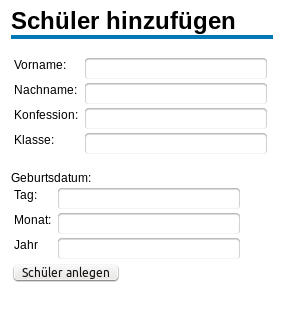
\includegraphics[scale=0.6]{img/UserAnlegen_KuWaSys.png}
 \end{center}
 \caption[\textbf{KuWaSys: User anlegen}]{KuWaSys: User anlegen}
 \label{fig:UserAnlegen_KuWaSys}
\end{figure}


% User anlegen: Lehrer
\begin{figure}[H]
 \begin{center}
   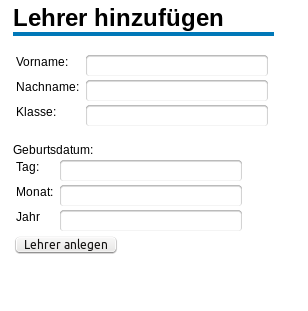
\includegraphics[scale=0.6]{img/LehrerAnlegen_KuWaSys.png}
 \end{center}
 \caption[\textbf{KuWaSys: Lehrer anlegen}]{KuWaSys: Lehrer anlegen}
 \label{fig:LehrerAnlegen_KuWaSys}
\end{figure}

textbf{Sonderfunktion: CSV-Import}

Eine Besonderheit der Benutzerverwaltung ist der Import von Userdaten über \ac{CSV}-Dateien. Diese Funktion war im Sinner der Projektarbeit nicht gefordert erleichtert aber die Arbeit mit dem System ungemein. Da jedes Jahr, zum Schuljahresbeginn, neue Schüler in das Kursplanungs- und Kurswahlsystem mit aufgenommen werden müssen wäre der Aufwand einzelne Benutzer hinzuzufügen zu groß und langwierig. Außerdem werden CSV-Dateien auch von gängigen Tabellenkalkulationsprogrammen unterstützt.

Als Vorlage für erste Importversuche diente die aktuelle Schülerliste im CSV-Format. Diese enthielt Daten in der Form:
%% Listing: CSV Schüler
	\lstinputlisting[label={lst:schiller_schueler.csv},
	caption={Beispiel einer CSV-Datei mit User Informationen},
	frame=tlbr, 
	language=java, 
	breaklines=true, 
	numbers=left, 
	numberstyle=\tiny, 
	stepnumber=1, 
	numbersep=5pt, 
	basicstyle=\small\ttfamily,
	showstringspaces=true,
	keywordstyle=\bfseries\color{lila}, 
	backgroundcolor=\color{lightgrey}]{listings/schiller_schueler.csv}

Mit Hilfe dieser Datei konnte ein Parser entworfen werden. Umgesetzt wurde der Parser mit der JAVA-Klasse \texttt{StringTokenizer}, um Tokens zu definieren und nach ihnen zu selektieren, und mit der Klasse \texttt{BufferedReader} und \texttt{InputStreamReader}, um die CSV-Datei überhaupt erst einlesen zu können. 

Der \prettyref{lst:ImportBean.java} zeigt die ManagedBean-Klasse \texttt{importBean} mit der Methode \texttt{doImport()}, die den komplettem Parse-Vorgang einer CSV-Datei steuert.
Die wichtigsten Zeilen des Quellcodeausschnitts sollen kurz erläutert werden:
\begin{itemize}
  \item[Zeile]
  \item[08:] Initialisierung der String-Variablen
  \item[23:] Beginn des Parsing-Vorgangs: Solange die CSV-Datei weitere Zeilen enthält
  \item[25:] Initialisierung des StringTokenizers (Zeilen und Angabe des Trennzeichens)
  \item[26:] Zeilenweise Tokens auswählen, solange weitere Tokens existieren
  \item[28:] Switch-Case fängt Integer-Wert der Tokens ab und weist die Werte den richtige Strings zu
  \item[47:] Aufruf der Methode \texttt{addUser} der \texttt{DatabaseHandler}-Klasse, die als Paramter die ausgelesenen Informationen der CSV-Datei enthält und einen neuen User im System anlegt
\end{itemize}

Wie unschwer zu erkennen ist, ist der Parser sehr einfach gestrickt. Es reicht anzugeben welche Trennzeichen zwischen den Daten benutzt werden (Obwohl der Namen CSV als Trennzeichen das Komma suggeriert, können als Trennzeichen zumindest auch Semikoli verwendet werden).
Weiter ist es ausreichend zu wissen wann die CSV-Datei endet und schlussendlich wie die Reihenfolge, der Werte die ausgelesen werden sollen, ist.

%% Listing: CSV Schüler - Parser
	\lstinputlisting[label={lst:ImportBean.java},
	caption={CSV-Datei Parser-Methode},
	frame=tlbr, 
	language=java, 
	breaklines=true, 
	numbers=left, 
	numberstyle=\tiny, 
	stepnumber=1, 
	numbersep=5pt, 
	basicstyle=\small\ttfamily,
	showstringspaces=true,
	keywordstyle=\bfseries\color{lila}, 
	tabsize=2,
	backgroundcolor=\color{lightgrey}]{listings/ImportBean.java}

\subsection{Kursverwaltung}

Neben dem Anlegen von neuen Benutzern, muss das System auch die Funktionalität besitzen, neue Kurse hinzuzufügen.

%%
\todo[size=\small, color=red!40]{Kurs anlegen (Lehrer)/Kurs aktivieren (Admin)/Kurs wählen (Schüler) !!!auch Diagramm!!!}
%%

Darstellung des Stundenplans:
\begin{figure}[H]
\centering
\begin{tikzpicture}[x=\daywidth, y=-1cm, node distance=0 cm,outer sep = 0pt]
% Style for Days
\tikzstyle{day}=[draw, rectangle,  minimum height=1cm, minimum width=\daywidth, fill=yellow!20,anchor=south west]
% Style for hours
\tikzstyle{hour}=[draw, rectangle, minimum height=1 cm, minimum width=1.5 cm, fill=yellow!30,anchor=north east]

% Styles for events
% Dauer Stunden
\tikzstyle{hours}=[rectangle,draw, minimum width=\daywidth, anchor=north west,text centered,text width=5 em]
\tikzstyle{1hour}=[hours,minimum height=1cm]
\tikzstyle{2hours}=[hours,minimum height=2cm]
\tikzstyle{3hours}=[hours,minimum height=3cm]

% Style der Fächer
\tikzstyle{Kern}=[2hours,fill=green!20]
\tikzstyle{Kurs1}=[2hours,fill=red!20]
\tikzstyle{Kurs2}=[2hours,fill=blue!20]
\tikzstyle{Kurs3}=[2hours,fill=blue!10]
\tikzstyle{Kurs4}=[2hours, pattern=north east lines, pattern color=magenta]
\tikzstyle{Kurs5}=[3hours, pattern=north west lines, pattern color=magenta!60!white]s
\tikzstyle{Planche}=[1hour,fill=white]

% Positioning Tag/Stunden
\node[day] (mo) at (1,8) {Montag};
\node[day] (di) [right = of mo] {Dienstag};
\node[day] (mi) [right = of di] {Mittwoch};
\node[day] (do) [right = of mi] {Donnerstag};
\node[day] (fr) [right = of do] {Freitag};

\node[hour] (8-9) at (1,8) {8-9};
\node[hour] (9-10) [below = of 8-9] {9-10};
\node[hour] (10-11) [below= of 9-10] {10-11};
\node[hour] (11-12) [below = of 10-11] {11-12};
\node[hour] (12-13) [below  = of 11-12] {12-13};
\node[hour] (13-14) [below = of 12-13] {13-14};
\node[hour] (14-15) [below = of 13-14] {14-15};
\node[hour] (15-16) [below = of 14-15] {15-16};
\node[hour] (16-17) [below = of 15-16] {16-17};
\node[hour] (17-18) [below = of 16-17] {17-18};
\node[hour] (18-19) [below = of 17-18] {18-19};

% Position Fächer
\node[Kurs1] at (1,10) {Sport};
\node[Kern] at (1,8) {D/M/E};
\node[Kern] at (2,8) {Physique};
\node[Kern] at (4,8) {Physique};
\node[Kern] at (5,10) {Physique};
\node[Kern] at (2,10) {Maths};
\node[Kern] at (2,14) {Maths};
\node[Kern] at (3,8) {Maths};
\node[Kern] at (4,10) {Maths};
\node[Kern] at (5,8) {Maths};
\node[Kern] at (1,14) {TIPE};
\node[Kern] at (1,16) {TIPE};
\node[Kern] at (2,16) {TIPE};
\node[Kern] at (3,10) {TIPE};
\node[Kern] at (5,14) {TIPE};
\node[Kern] at (5,16) {TIPE};
\node[Kern] at (3,14) {Phys ou SI};
\node[Kern] at (3,16) {SI ou Phys};
\node[Kern] at (1,13) {Planche};
\node[Kern] at (1,18) {Colle};
\node[Kern] at (4,13.5) {Planche};

\end{tikzpicture}
\caption[\textbf{Netzwerkstruktur der Schillerschule Aalen}]{Netzwerkstruktur der Schillerschule Aalen}
\label{fig:Stundenplan}
\end{figure}

\subsubsection{Spezielle Daten eines Kurses}

Der Aufbau eines Kurses im System, wie aus dem ER-Modell in \prettyref{fig:ERModell} entnommen werden kann, besteht im Grunde aus einer Nummer, einem verantwortlichen Lehrer, einer Beschreibung, einem Termin, Information des dazugehörigen Fächerverbunds  und einer Teilnehmeranzahl. Allein mit diesen Information könnte ein Kurs im System dargestelltn werden. Hierbei werden jedoch die restlichen Attribute vernachlässigt. Diese sollen im folgenden näher zur Sprache kommen.  

Da die angebotenen Kurse im System nun verschiedenen Abhängigkeiten haben können und eventuell bestimmte Vorraussetzungen erfüllen können müssen, wurde eine Möglichkeit gesucht diese Kurse möglichst einfach im System abzubilden. 
Einfach bedeutet an dieser Stelle, dass die Darstellung eines Kurses für alle Rollen gleichermaßen zur Verfügung stehen muss und außerdem Interaktionen mit ihnen unterstützt.
Hierbei müssen die oben vernachlässigten Attribute beachtet werden. 

Attribute die hierbei einer Rolle spielen sind: (Vrgl. ER-Modell in \prettyref{subsec:ERModell})
\begin{itemize}
  \item Sportkurs
  \item Konfession (derzeit EV, RK und Ethik)
  \item Pflichtkurse
\end{itemize}

\textbf{Sportkurse}

Hierbei handelt es sich um ein Attribut, also einer Spalte in der Kurs-Tabelle, die den Datentyp \texttt{boolean} besitzt.
Beim Anlegen hat der Lehrer oder der Admin die Möglichkeit dieses Attribut des zu erstellenden Kurses zu setzen, wie es die grüne Markierung in \prettyref{fig:KursAnlegen_KuWaSys} zeigt.

Das anlegen des Sportkurs-Flags in der DB ist trivial und wird daher nicht weiter betrachtet.

Von einer Besonderheit bei Sportkursen kann gesprochen werden wenn zusätzlich die Fächerverbünde und Pflichtkurse mitbetrachtet werden.
Für gewöhnlich wird ein Sportkurs dem Fächerverbund \ac{MSG} zugeordnet. Es kann allerdings vorkommen, dass ein Kurs als Sportkurs angelegt wird, aber keinen Pflichtkurs darstellt.  
Pflichtkurse werden am Ende dieses Abschnitts noch behandelt.

Beim Anlegen hat der Lehrer oder der Admin die Möglichkeit dieses Attribut des zu erstellenden Kurses zu setzen, wie es die grüne Markierung in \prettyref{fig:KursAnlegen_KuWaSys} zeigt.


\textbf{Religionsunterricht}

Eine richtige Besonderheit stellt das Anlegen eines Religionskurses dar.
Das Anlegen eines Religionskurses (grüne Markierung in \prettyref{fig:KursAnlegen_KuWaSys}) wird über einfach Selectboxen realisiert. Der Inhalt der Selectboxen wird dazu automatisch angelegt. Wie dies gewährleistet wird soll nun näher besprochen werden.

Wie bereits in \prettyref{fig:UserAnlegen_KuWaSys} gezeigt wurde, wird beim Anlegen eines Users im System, eine Konfessionszugehörigkeit beigefügt. Dieses Feld kann vom Admin beliebig ausgefüllt werden. 
Dieser beliebige String wird in die Tabelle 'Kurskonfession' eingetragen und wird später, durch die Auswahl beim Anlegen eines Kurses, als Fremdschlüssel in der 'Kurs'-Tabelle gespeichert.
Der Inhalt der Selectboxen die zur Verfügung stehen, ist also immer komplette Inhalt der Kurskonfession-Tabelle.




Diese Art der Lösung soll in Zukunft alternative Unterrichte zulassen können.

% Kurs anlegen
\begin{figure}[H]
 \begin{center}
   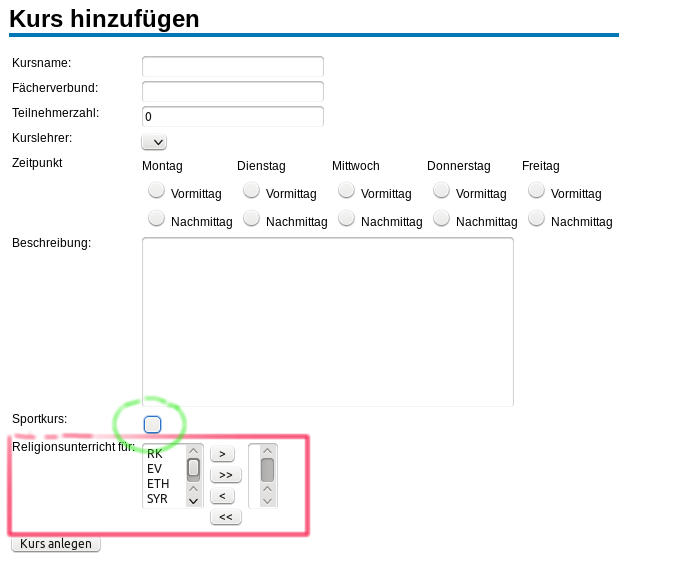
\includegraphics[scale=0.6]{img/KursAnlegen_KuWaSys.png}
 \end{center}
 \caption[\textbf{KuWaSys: Kurs anlegen}]{KuWaSys: Kurs anlegen}
 \label{fig:KursAnlegen_KuWaSys}
\end{figure}

\textbf{Pflichtkurse}

Ähnlich wie bei Sportkursen handelt es sich hierbei um ein Attribut, also ebenfalls einer Spalte in der Kurs-Tabelle, die auch den Datentyp \texttt{boolean} besitzt.
Im Gegesatz zu Sportkursen wird das Pflichtkurs-Flag allerdings nicht beim Anlegen eines Kurses gesetzt. Es kann nur vom Admin bestimmt werden, ob ein Kurs ein Pflichtkurs ist oder nicht. Festlegen kann er dies in der Kursverwaltung in der Phase der Kursplanung.

Die \prettyref{fig:KursVerwalten_KuWaSys} zeigt einen Ausschnitt der Kursverwaltung aus Sicht des Admins.
Der Admin hat die Möglichkeit Kurse zu aktivieren, also den Schülern die Kurse zur Kurswahl zur Verfügung zu stellen oder bereits aktivierte Kurse wieder zu deaktivieren.
Darüberhinaus legt der Admin die Pflichtkurse fest.

% Kurs verwalten
\begin{figure}[H]
 \begin{center}
   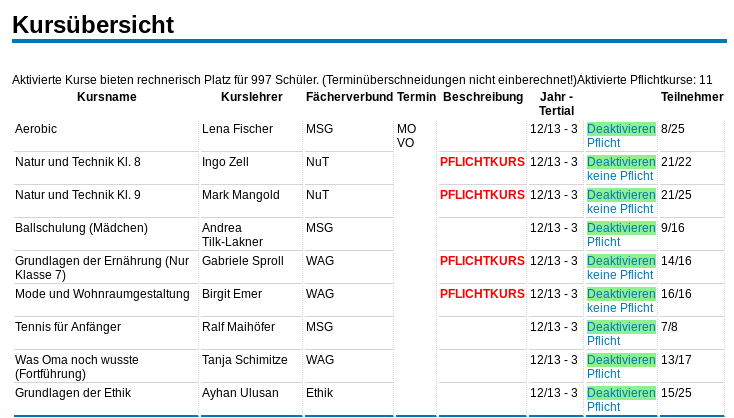
\includegraphics[scale=0.6]{img/KursVerwalten_KuWaSys.png}
 \end{center}
 \caption[\textbf{KuWaSys: Kurse verwalten}]{KuWaSys: Kurse verwalten}
 \label{fig:KursVerwalten_KuWaSys}
\end{figure}

\subsubsection{Benutzerunterstützung}
%%
\todo[size=\small, color=red!40]{Anzeige der abgehandelten Kurse/Fächerverbünde etc... (Schüler bzw. Admin)}
%%%%
\todo[size=\small, color=orange!40]{Screenshot}
%%


\subsection{Systemverwaltung}
%%
\todo[size=\small, color=red!40]{Umsetzung der Stati des Systems}
%%%%
\todo[size=\small, color=orange!40]{Screenshot}
%%



\section{Tests, Fehlervermeidung und Qualitätssicherung}\label{sec:Testing und Debugging}

%% Einleitung %(
Dieser Abschnitt widmet sich dem Thema der Testverfahren in Softwareprojekten mit dem Schwerpunkt bezogen auf das entwickelte JSF-Projekt 'KuWaSys'.
Zuerst sollen die allgemein geltenden Grundlagen angesprochen werden, darauf aufbauend werden die im Projekt verwendeten Testverfahren näher erläutert. 

Tests lassen sich in der Software Entwicklung nach ihrer Art und Weise klassifizieren.
Auf der einen Seite steht die Konstruktive-Qualitätssicherung auf der anderen Seite die Analytische.

Zu den Konstruktiven-Qualitätssicherungsmaßnahmen zählen Durchführungen während dem und am Entwicklungsprozesses selbst:
\begin{itemize}
  \item Checklisten
  \item Programmier-Guidlines
  \item Templates
\end{itemize}

Die Analytischen-Qualitätssicherung, zu welchen Tests am Produkt gehören, können in zwei verschiedene Testverfahren eingeteilt werden. Hierbei handelt es sich um statische und dynamische Tests.
Verfahren die hierzu eingesetzt werden sind für statische Test:
\begin{itemize}
  \item Statische Analyse
  \item Reviews
\end{itemize}

Im Sinne der statischen Analyse wurden während der Entwicklung folgende Punkte überprüft:
\begin{itemize}
  \item existieren Klassen bzw. Methoden
  \item sind die Scopes der ManagedBeans korrekt
  \item sind ManagedBeans mit dem Scope \texttt{Session} und \texttt{Application} serialisierbar
  \item haben ManagedBeans Properties die benötigten Setter-/Getter-Methoden
\end{itemize}

Und für dynamische Test beispielsweise:
\begin{itemize}
  \item \gls{Blackbox}-Testverfahren
  \item \gls{Whitebox}-Testverfahren
\end{itemize}


Die Planung und Strukturierung der Durchführung von Softwaretests, aber auch die Überlegung von Testfällen die am System geprüft werden sollen, stellen einen äußerst wichtigen Prozess der Softwareentwicklung dar.
Diese Schritte fließen bestenfalls zu Beginn des Projekts, in der Planungsphase, mit ein. (\cite{SPM}, ab Seite 5undzwölfzig)

%% TODO evtl hier checkliste?!
Als geplante Tests am fertigen System wurden die folgenden vorgesehen, die im Checklisten-Verfahren abgearbeitet wurden:
\begin{itemize}
	\item Tests bezügliche der Interaktion am System (mit Testpersonen und deren Feedback)
	\begin{itemize} 
		 \item prüfen der Übersichtlichkeit aller Benutzergruppen
		 \item Kontrolle des Seitenaufbaus und der Strukturierung für effizientes Arbeiten
	\end{itemize}
	\item Testeingaben in Textfelder
	\begin{itemize} 
		 \item Tests der Schnittstellen und der übergebenen Parameter nach Datentyp
		 \item Abklärung von eventuellen Encoding-Problemen
	\end{itemize}
	\item Funktionalitätstests aller Schaltflächen
	\begin{itemize} 
		 \item absichern von korrekten Systemereignissen bzw. -funktionen
		 \item Kontrolle der übergebenen Werte und Datentypen, um Fehlbelegungen auszuschließen
	\end{itemize}
	\item Konsistenz der Datenbank 
	\begin{itemize} 
		 \item Abfragen mit Hinblick auf Eindeutigkeit, bspw. bei \texttt{UNIQUE-Constraints} sowie \texttt{PRIMARY KEY-} und \texttt{FOREIGN KEY-Constraints}
		 \item Überprüfung der verwendeten Datentypen im System
	\end{itemize}
\end{itemize}

Im folgenden sollen Tests im Zusammenhang mit der Softwarequalitätssicherung und die Umsetzung im 'KuWaSys' näher betrachtet werden.

Der Stellenwert der Qualitätssicherung von Software hat in der heutigen Zeit einen so großen Stellenwert angenommen, dass es mittlerweile sogar ISO-Normen gibt, genauer gesagt die ISO-Norm 9126 - für Qualität in Software. Diese Norm enthält grundlegende Bestimmungen über Effizienz, Funktionalität, Zuverläsigkeit, Benutzbarkeit, Portabilität und Wartbarkeit. 
Die genauen Details der Definitionen werden hier nicht weiter erwähnt da diese über das Thema der Projektarbeit hinaus gehen würden. Eine gute und vollständige Zusammenfassung der gesamten Norm ist jedoch unter \cite{WikiISO9126} zu finden.

% ISO 9126 MindMap
\begin{figure}[H]
\centering\begin{tikzpicture}[mindmap,
  level 1 concept/.append style={level distance=130,sibling angle=30},
  extra concept/.append style={color=blue!50,text=black}]

\begin{scope}[mindmap, concept color=green, text=white]
\node [concept]at (-2,1) {ISO 9126}[clockwise from=-5]
    child [grow=10] {node [concept] (E) {Effizienz}}
    child {node [concept] (F) {Funktionali-tät}}
    child [grow=240] {node [concept] (E) {Zuverläsig-keit}}
    child [grow=110] {node [concept] (B) {Benutzbar-keit}}
    child [grow=60] {node [concept] (P) {Portabilität}}
    child [grow=280] {node [concept] (W) {Wartbarkeit}};
\end{scope}
\end{tikzpicture}
\caption[\textbf{ISO Norm 9126}]{ISO Norm 9126}
\label{fig:Projekt_Mindmap}
\end{figure}
%)

%% Test/Qualität im Projekt %(
Grundsätzlich wurden allgemein gültige Richtlinien und Code-Konventionen von JSF im Projekt umgesetzt. Dies erhöht zum eine die Übersichtlichkeit des gesamten Projekts und wirkt sich postiv auf die kooperierende Entwicklung aus. Dadurch werden gleichermaßen qualitätsichernde Maßnahmen ergriffen wie auch Fehleranfälligkeiten minimiert.  

Das Benutzen von Templates, welche während der Implementierungsphase eingesetzt wurden, stellt ebenfalls eine Technik dar, die zur Fehlervermeidung beiträgt. Das verwendete Design des 'KuWaSys' musste somit nur einmal definiert und getestet werden und konnte anschließend beliebig oft weiter verwendet werden ohne dabei das Risiko eingehen zu müssen dass das Design inkonsistent wird oder dass sich neue Fehler im Projekt einschleichen könnten. 

Um Laufzeittests durchzuführen wurden FacesMessages, über den entsprechenden Import der Klasse \texttt{javax.faces.application.FacesMessage} benutzt, die Gleichzeitig die Fehleranalyse mit Hilfe der Konsole erleichtern.
Ein Beispiel solcher Messages ist in \prettyref{lst:FacesMessages} dargestellt. Im Falle eines Fehlers würde der ausgeführte \texttt{Catch}-Block, über den benutzerdefinierten FacesMessages-Befehl, eine Ausgabe produzieren.
Nebenbei sei noch eine weitere Besonderheit in JSF angemerkt:
Während der Status 'Development' im  Projekt steht, welcher in der \texttt{POM.xml} festgelegt wird, werden Fehler für bestimmte Funktionen automatisch ausgegeben. Dies ist vor allem bei einem Release zu beachten und vorher abzuändern.

%% Listing: FacesMessages
	\lstinputlisting[label={lst:FacesMessages},
	caption={Debugging mit FacesMessages},
	frame=tlbr, 
	language=java, 
	breaklines=true, 
	numbers=left, 
	numberstyle=\tiny, 
	stepnumber=1, 
	numbersep=5pt, 
	basicstyle=\small\ttfamily,
	showstringspaces=true,
	keywordstyle=\bfseries\color{lila}, 
	tabsize=2,
	backgroundcolor=\color{lightgrey}]{listings/FacesMessages.java}
	
Wie in der folgenden \prettyref{figmin:SchulerImportieren_KuWaSys} zu erkennen ist, wird die Message während der Laufzeit ausgeführt, wie bei diesem missglückten Datei-Upload.

% Kurs anlegen
\begin{figure}[H]
 \begin{center}
   
\includegraphics[scale=0.8]{img/SchulerImportieren_KuWaSys.png}
 \end{center}
 \caption[\textbf{KuWaSys: Datei-Upload Fehler beim Schüler Importieren}]{KuWaSys: Datei-Upload Fehler beim Schüler Importieren}
 \label{figmin:SchulerImportieren_KuWaSys}
 \label{fig:SchulerImportieren_KuWaSys}
\end{figure}

Diese Tests erwiesen sich bei Datenbankabfragen als sehr hilfreich, da nicht erst aufwändige Oberflächen umgesetzt werden müssen um Fehler zu erkennen, sondern Daten sofort auf ihre Richtigkeit hin geprüft werden können.
Diese Fehler sind gleich zu Beginn der Implementierung aufgefallen, da es sich hier vor allem um Fehler die während der Modellierungs- beziehungsweise (bzw.) Designphase entstanden sind, handelt. Diese Fehler sind mit FacesMessages relativ schnell auszumachen und ebenso schnell korrigiert. Beispiele solcher Fehler sind:
\begin{itemize}
  \item falsche Überlegungen zu den Datentypen in der \ac{DB}
  \item schlecht definierte Schnittstellen
  \item Inkonsitenz im Design 
\end{itemize}

Eine weitere Möglichkeit, Fehler in einer Webapplikation zu entdecken ist das benutzen von selbstdefinierten Server-Logs.
Hierzu wurde von uns die Klasse \texttt{import java.util.logging.Logger} verwendet. Der \prettyref{lst:Logger} zeigt wie beispielsweise ein \texttt{Catch}-Block  mitgeloggt werden kann.

%% Listing: Logging
	\lstinputlisting[label={lst:Logger},
	caption={Server-Logging in JSF},
	frame=tlbr, 
	language=java, 
	breaklines=true, 
	numbers=left, 
	numberstyle=\tiny, 
	stepnumber=1, 
	numbersep=5pt, 
	basicstyle=\small\ttfamily,
	showstringspaces=true,
	keywordstyle=\bfseries\color{lila}, 
	tabsize=2,
	backgroundcolor=\color{lightgrey}]{listings/Logger.java}

Da ständig auf einem aktiven System (Corporate Identity) - glossarntwickelt und getestet wurde konnten Tester aus dem Umfeld der Schule für diesen Zweck eingesetzt werden.
Dies erwies sich vor allem beim Entwickeln des Oberflächendesigns als Vorteil. Es konnten Wünsche von Lehrern und Schülern direkt berücksichtigt und umgesetzt werden.
Hier bekommen besonders Checklisten und Reviews einen hohen Stellenwert. Nur durch regelmäßige gemeinsame Treffen konnten Projekttermine (neu-)definiert werden.

Im Hinblick auf die vorher besprochene ISO-Norm 9126 erfüllt das Kurswahlsystem alle Bestimmungen. Jedoch muss fairnesshalber dazu gesagt werden, dass Dinge wie Effizienz in Software nie mit einem genauen Maß gemessen werden kann, da viele Faktoren ein Rolle spielen.
Zum Beispiel müssen bei gewissen Datenstrukturen Laufzeiteinschränkungen in Kauf genommen werden wenn sich dadurch die Darstellung effizienter umsetzen lässt. Andererseits können natürlich schneller Datenstrukturen oder Algorithmen in einer viel langsameren Darstellung resultieren.
Dasselbe gilt für die Zuverläsigkeit. Natürlich ist das Kurswahlsystem so entworfen worden, dass die Erreichbarkeit und Nutzbarkeit jederzeit gegeben ist. Aber auch hier unterliegt das System mehreren außenstehenden Faktoren auf die ein Entwickler niemals Einfluss nehmen kann.
%)

%% JSFUnit %(
Selbstverständlich können für den Java Server Faces Standard auch Tests implementiert werden. Diese werden für gewöhnlich bei den Dynamischen-Test angesiedelt. Von uns wurden keine spezielle Frameworks zur Realisierung von Tests verwendet. Vollständigkeitshalber soll allerdings eines der interessantesten Vertreter von Testinstrumenten für JSF erwähnt werden:

Hierbei handelt es sich um \gls{JSFUnit}, welches auf dem bekannten JAVA-Testframework \gls{JUnit} aufbaut. Tests können hierzu über die JSFUnit-Konsole oder durch den Aufruf einer Testseite ausgeführt werden. Testmöglichkeiten sind Wert- und Zustandsänderungen in ManagedBeans, setzen von Navigationszielen oder über FacesMessages.
Eine besondere Art der Tests sind die 'Acrylic Box'-Testings. Diese verbinden Whitebox und Blackbox-Testverfahren und werden bei den dynamischen Tests eingestuft.
Nähere Informationen sind unter \cite{JSFUnit01} zu finden.
%)

Zuletzt soll noch hinzugefügt werden, dass auch ausführliche Tests keine Garantie auf eine vollständige Fehlerfreiheit geben.
Allerdings helfen Tests die Fehler möglichst gering zu halten und steigern die Qualität der Software um ein gewisses Maß.
Obwohl das Projekt ausführlichst getestet wurde kann es dennoch nicht ausgeschlossen werden, dass noch welche existieren. 

\newpage

\section{Fazit und Ausblick}\label{sec:Fazit und Ausblick}

%% Einleitung %(
Abschließend soll ein gesamtheitlicher Überblick der Projektarbeit gegeben werden, indem das entwickelte System komplett betrachtet wird.
Für ein sinnvolles Fazit sollen zwei wesentliche Punkte angesprochen werden:
\begin{enumerate}
  \item Beurteilung der Nutzbarkeit und die gesamtheitliche Umsetzung des Projekts
  \item Beurteilung der eingesetzten Technologien
\end{enumerate}

%%% TODO
Vor allem beim zweiten Punkt sollen zwei weitere Kriterien differenziert werden:
Beim Einen handelt es sich um das Kriterium der Verwendbarkeit der Technologie für den Entwickler, hier ist dieser in einer aktiven Rolle zu sehen. 
Beim Anderen handelt es sich vor allem um eine Betrachtung der Technologie in Punkten wie Komplexität, Verwendbarkeit und Spezifiktaion, in welchen der Entwickler lediglich nur eine passive Rolle einnehmen kann.
%)

%% Betrachtung System %(
An oberster Stelle stand das Ziel, die Anforderungen an das System erfolgreich umzusetzen.
Das positive Resultat kann der engen Kooperation während der Implementierungsphase und der ausgiebigen Problemabgrenzung, wie grob zu Beginn in \prettyref{subsec:Problemstellung und -abgrenzung} beschrieben ist, angerechnet werden.
Vor allem die ersten drei bis vier Wochen nach Projektstart dienten dazu, die Ziele zu definieren. Beinahe jede Woche hielten wir mit den verantwortlichen Personen (in \prettyref{subsec:Verantwortliche Personen} namentlich aufgeführt) der Schillerschule Aalen ein Projektmeeting ab, in welchem Ergebnisse des Projektfortschritts präsentiert und diskutiert wurden.
Ein weiterer wichtiger Punkt, der zu diesem Ergebnis geführt hat, war das entgegengebrachte Vertrauen von Seiten der Schule.

Wie es \prettyref{secmin:Implementierung} zu entnehmen ist, wurden alle Punkte der Systemanforderung erfüllt. Darüberhinaus wurden sogar zusätzliche Funktionalitäten implementiert.
Hier wäre die Umsetzung der Export-/Importfunktionen von CSV Dateien, Funktionalität die Userdaten betreffen (bspw. Passwort-Neugenerierung) und die komplette Umsetzung der \ac{IT}-Infrastruktur der Schillerschule genannt. 
Insofern muss der entstandene Fortschritt mit dem neuen Kurswahlsystem im Hinblick auf das erste Kursverwaltungstool gesehen werden.

Das größte Manko, der nicht unterstützte Multi-User Betrieb und die Einschränkung der Lauffähigkeit begrenzt auf ein System, wurden beseitigt. Ebenso wurde mehr Wert auf ein gewisses Maß an Selbstverantwortung bei Lehrern aber auch Schülern gelegt.
Im Idealfall wird der Admin nur noch zur Konfiguration des Systems und in Problemfällen aktiv.
Auch die Verwaltungsassistenz wurde im neuen Tool erfolgreich umgesetzt. So werden Daten die für die Kursplanung wichtig sind vom System ermittelt und den Benutzern zur Verfügung gestellt. 
Ebenso wurde der entwickelte Arbeitsablauf für Lehrer und Schüler umgesetzt und die Kommunikation untereinander dadruch verbessert indem Probleme Systembedingt abgefangen werden können.

Als dritter und letzter Verbesserungsschritt ist die neugestaltung der Oberfläche zu sehen. Diese wurden mit Hilfe von bereits erprobten und bewährten Gestaltungselementen, die aus dem Gebiet der \ac{MCI} bekannt sind, umgesetzt. \cite{DahmMCI}.

Die eindeutige Abgrenzung von Menü, Informationen und Arbeitsbereich sind gleichermaßen umgesetzt wie die Darstellung aller Systemrelevanter Daten wie es in der Anforderung gewünscht war.

Zukünftige Erweiterungen sind im System vorgesehen. Aufgrund der Modularität die sich strikt durch das ganze System zieht werden diese auch realisierbar sein.

Realisierbare Erweiterungen könnten sein:
\begin{itemize}
  \item eine Änderungsinformationsanzeige für Admins bei bestimmten Systemereignissen, sodass ohne fundierte \ac{IT}-Kenntnisse, Fehler an Server und Datenbank frühzeitig erkannt werden können
  \item eine interne Kommunikationsplattform für den Austausch von Informationen zwischen Lehrern und Administrator und zwischen Schülern - und Lehrern  
  \item Erweiterungen wie Kalenderfunktionen, Stundenplan-Generierung,....
\end{itemize}
  
Manche der aufgeführten Vorschläge werden bereits im Momentanen Stand der Entwicklung, ansatzweise umgesetzt. 
Aufgrund der Fülle und Diversität der Art an Anforderungen die zu Beginn an das Projekt festgehalten wurden fanden diese jedoch in der Projektarbeit bedauerlicherweise fast keinen Platz.
%)

%% Technologien %(
Es hat sich gezeigt, dass \ac{JSF} ein gut definierter Webentwicklungsstandard geworden ist.
Aufgrund der Einfachheit der Handhabung kommen Anfänger der Webentwicklung aber auch Fortgeschrittene gut damit zurecht und voll auf ihre Kosten.
Je nach Komplexität der Interaktion mit dem System sind JAVA Kenntnisse erfoderlich, in jedem Falle aber sinnvoll. 
Eine Entwicklung die ihren Schwerpunkt auf das Design oder generell die Darstellung legt benötigt nur sehr wenige Kenntnisse im Bereich JAVA dafür aber Kenntnisse einer Seitendeklarationssprache wie HTML oder JSP.
Sollen aber, wie es in dieser Projektarbeit der Fall war, Daten aus einer Datenbank verändert oder in eine Datenbank geschrieben werden sind fundierte Kenntnisse der Softwareentwicklung mit JAVA notwendig.

Zur verwendeten Datenbank lassen sich keine besonders wichtigen oder bahnbrechenden Aussagen machen. PostgreSQL hat sich bereits über Jahre etabliert und wurde stetig weiter verbessert. 
Die Verwendung für unerfahrene Nutzer stellt nach einer kurzen Einarbeitung kein größeres Problem dar und kann somit nur weiterempfohlen werden. 
 
Die Entwicklungsunterstützung mit Maven ist bei Projekten dieser Art eine sehr große Hilfe.
Ohne eine Verwaltungshilfe der Bibliotheken, Pakete oder der Projektverweise kann ein Projekt in dieser Größenordnung schnell in einen Bereich kommen, in welchem plötzlich der Verwaltungsaufwand steigt und schnell zur Hauptaufgabe des Entwicklers wird.
Der Fokus schweift immer öfters vom Projekt ab. Das Resultat davon ist:
\begin{itemize}
	\item ein höherem Zeitaufwand für das Beheben von entstandenen Problemen durch die Verletzung von Abhängigkeiten 
	\item mehr Fehler im Programmcode der wiederrum auch zu längeren Testphasen führt
	\item teilweise leidet die Qualität des entstanden Codes 
\end{itemize}
Für viele Entwickler (oder Projektleiter) ist dies ein stark vernachlässigtes Thema.
Ohne eine genaue Planung und ohne konkrete Vorstellungen lässt sich jedoch ein Softwareprojekt, egal welcher Größe, meist nie korrekt realisieren.  
Dies sind alles Gründe die dafür gesorgt haben, dass das Projekt unter zu Hilfenahme des Development-Tools Maven umgesetzt wurde.
Die Softwareentwicklung bleibt im Vordergrund.
%)

%% Rückblick %(
Rückblickend kann dem Projekt ein voller Erfolg zugeschrieben werden.
Funktional genügt das System den Anforderungen und sogar darüber hinaus. Der zeitliche Aufwand war sehr hoch, aber im Rahmen des Möglichen, sodass nicht von 'zu viel' gesprochen werden kann.
Zeitliche Einbußen musste dennoch hingenommen werden. So stellten vor allem das Testen und die Integration des Systems in die Infratruktur der Schule einen langwierigen Prozess dar und sprengte den geplanten Rahmen.
Letztenendes sorgten Dinge wie die Anleitung, die technische Dokumentation und diese Ausarbeitung der Projektarbeit für den nötigen Abschluss des Projekts.

%)

\newpage

%% Neuer Style
\pagestyle{fancy}
	\renewcommand{\sectionmark}[1]{\markboth{#1}{}}
	\fancyhf{}
	\fancyhead[L]{ { }\leftmark}
	\fancyhead[R]{\thepage}
	\renewcommand{\headrulewidth}{0.4pt}
	%\pagenumbering{roman}

Die ist in \prettyref{sec:Anhang} zu finden.
	
\begin{appendix}
\section{Anhang}\label{sec:Anhang}

\subsection{Inhalte der CD}
Folgende Inhalte sind auf der abgegebenen CD zu finden:

\begin{itemize}
  \item Kopie der Entwicklungsumgebung Eclipse 10.04 Juno mit allen Plugins
  \item virtuelles Abbild des konfigurierten Servers
  \item diese Ausarbeitung
  \item Dokumentation in JAVAdoc
  \item Benutzerhandbuch für das 'KuWaSys'				%%
  \item Kopien der verwendeten bzw. zitierten Websites\todo[size=\small, color=green!40]{Fragwürdig!!!} 
\end{itemize}											%%

\subsection{Konfiguration und Installation}

\subsubsection{Maven}

Maven Befehle listings

\subsubsection{Apache Tomcat 7}

Hier soll in einer kurzen Darstellung die Administration des Apache Tomcat 7 und dessen wichtige Dateien und Verzeichnisse 

\textbf{}
Apache Tomat7 Befehle Listings

Verzeichnisse

\subsection{Zugangsdaten für den Server und das System}

\textbf{Server Zugangsdaten}

% Zugangsdaten
\begin{table}[H]
\begin{center}
	\begin{tabular}{|l|l|l||}\hline
		\textbf{Rolle} & \textbf{Username} & \textbf{Passwort} \\ \hline
		Admin & ijcy & 12kuwasys34 \\ \hline \hline
	\end{tabular}
	\caption{Server Zugangsdaten}
\end{center}
\end{table}

\textbf{Datenbank Zugangsdaten}

% Datenbank Zugangsdaten
\begin{table}[H]
\begin{center}
	\begin{tabular}{|l|l|l||}\hline
		\textbf{Rolle} & \textbf{Username} & \textbf{Passwort} \\ \hline
		Admin & ijcy & 12kuwasys34 \\ \hline
		Admin & postgres & 12kuwasys34 \\ \hline \hline
	\end{tabular}
	\caption{Datenbank Zugangsdaten}
\end{center}
\end{table}

\subsection{Gesetzesauszüge}\label{subsec:Gesetz}

Auszug aus dem \ac{TMG}:

\textbf{§ 5 Allgemeine Informationspflichten}
\begin{itemize}
\item[(1)] Diensteanbieter haben für geschäftsmäßige, in der Regel gegen Entgelt angebotene Telemedien folgende Informationen leicht erkennbar, unmittelbar erreichbar und ständig verfügbar zu halten:
  \begin{enumerate}
    \item den Namen und die Anschrift, unter der sie niedergelassen sind, bei juristischen Personen zusätzlich die Rechtsform, den Vertretungsberechtigten und, sofern Angaben über das Kapital der Gesellschaft gemacht werden, das Stamm- oder Grundkapital sowie, wenn nicht alle in Geld zu leistenden Einlagen eingezahlt sind, der Gesamtbetrag der ausstehenden Einlagen,
    \item Angaben, die eine schnelle elektronische Kontaktaufnahme und unmittelbare Kommunikation mit ihnen ermöglichen, einschließlich der Adresse der elektronischen Post,
    \item soweit der Dienst im Rahmen einer Tätigkeit angeboten oder erbracht wird, die der behördlichen Zulassung bedarf, Angaben zur zuständigen Aufsichtsbehörde,
    \item das Handelsregister, Vereinsregister, Partnerschaftsregister oder Genossenschaftsregister, in das sie eingetragen sind, und die entsprechende Registernummer,
    \item soweit der Dienst in Ausübung eines Berufs im Sinne von Artikel 1 Buchstabe d der Richtlinie 89/48/EWG des Rates vom 21. Dezember 1988 über eine allgemeine Regelung zur Anerkennung der Hochschuldiplome, die eine mindestens dreijährige Berufsausbildung abschließen (ABl. EG Nr. L 19 S. 16), oder im Sinne von Artikel 1 Buchstabe f der Richtlinie 92/51/EWG des Rates vom 18. Juni 1992 über eine zweite allgemeine Regelung zur Anerkennung beruflicher Befähigungsnachweise in Ergänzung zur Richtlinie 89/48/EWG (ABl. EG Nr. L 209 S. 25, 1995 Nr. L 17 S. 20), zuletzt geändert durch die Richtlinie 97/38/EG der Kommission vom 20. Juni 1997 (ABl. EG Nr. L 184 S. 31), angeboten oder erbracht wird, Angaben über
    \begin{itemize}
      \item[a)] die Kammer, welcher die Diensteanbieter angehören,
      \item[b)] die gesetzliche Berufsbezeichnung und den Staat, in dem die Berufsbezeichnung verliehen worden ist,
      \item[c)] die Bezeichnung der berufsrechtlichen Regelungen und dazu, wie diese zugänglich sind,
    \end{itemize}
    \item in Fällen, in denen sie eine Umsatzsteueridentifikationsnummer nach § 27a des Umsatzsteuergesetzes oder eine Wirtschafts-Identifikationsnummer nach § 139c der Abgabenordnung besitzen, die Angabe dieser Nummer,
    \item bei Aktiengesellschaften, Kommanditgesellschaften auf Aktien und Gesellschaften mit beschränkter Haftung, die sich in Abwicklung oder Liquidation befinden, die Angabe hierüber.
  \end{enumerate}
\item[(2)] Weitergehende Informationspflichten nach anderen Rechtsvorschriften bleiben unberührt.
\end{itemize}

Auszug aus dem \ac{RstV}:

\textbf{§ 55 - Informationspflichten und Informationsrechte}
\begin{itemize}
  \item[(1)] Anbieter von Telemedien, die nicht ausschließlich persönlichen oder familiären Zwecken dienen, haben folgende Informationen leicht erkennbar, unmittelbar erreichbar und ständig verfügbar zu halten:
  \begin{enumerate}
    \item Namen und Anschrift sowie
    \item bei juristischen Personen auch Namen und Anschrift des Vertretungsberechtigten.
  \end{enumerate}
  \item[(2)] Anbieter von Telemedien mit journalistisch-redaktionell gestalteten Angeboten, in denen insbesondere vollständig oder teilweise Inhalte periodischer Druckerzeugnisse in Text oder Bild wiedergegeben werden, haben zusätzlich zu den Angaben nach §§ 5 und 6 des Telemediengesetzes einen Verantwortlichen mit Angabe des Namens und der Anschrift zu benennen. Werden mehrere Verantwortliche benannt, so ist kenntlich zu machen, für welchen Teil des Dienstes der jeweils Benannte verantwortlich ist. Als Verantwortlicher darf nur benannt werden, wer
  \begin{enumerate}
    \item seinen ständigen Aufenthalt im Inland hat,
    \item nicht infolge Richterspruchs die Fähigkeit zur Bekleidung öffentlicher Ämter verloren hat,
    \item voll geschäftsfähig ist und
    \item unbeschränkt strafrechtlich verfolgt werden kann.
  \end{enumerate}
  \item[(3)] Für Anbieter von Telemedien nach Absatz 2 Satz 1 gilt § 9 a entsprechend.
\end{itemize}

\subsection{Verantwortliche Personen}\label{subsec:Verantwortliche Personen}

Ralf Meiser - Konrektor

Björn Bolch - 

Alexander Neugebauer - IT Systembeauftragter der Schillerschule Aalen

%% Abkürzungsverzeichnis
\newpage
\section{Akronyme}
\input{PA-01-Projekt_PDFVersion_KuWaSys.acronym}

%% Glossar

\newpage
\section{Glossar}
\glossary{
  name={entry name}, 
  description={entry description}
}
\printglossary[title={}] 

\end{appendix}

% Abbildungsverzeichnis
\newpage
\addcontentsline{toc}{section}{\textbf{Abbildungsverzeichnis}}
\listoffigures
\cleardoublepage

% Tabellenverzeichnis
\newpage
\addcontentsline{toc}{section}{\textbf{Tabellenverzeichnis}}
\listoftables
\cleardoublepage

% Quellcodeverzeichnis
\newpage
\addcontentsline{toc}{section}{\textbf{Quellcodeverzeichnis}}
\lstlistoflistings
\cleardoublepage

%% Literaturverzeichnis
\newpage
\addcontentsline{toc}{section}{\textbf{Literaturverzeichnis}}
\bibliographystyle{alphadin}	  
\bibliography{PA-01-Projekt_PDFVersion_KuWaSys}

%% Eidesstattliche Erklärung
\addcontentsline{toc}{section}{\textbf{Eidesstattliche Erklärung}}

\end{document} 


%% Glossar

\newpage
\section{Glossar}
\glossary{
  name={entry name}, 
  description={entry description}
}
\printglossary[title={}] 

\end{appendix}

% Abbildungsverzeichnis
\newpage
\addcontentsline{toc}{section}{\textbf{Abbildungsverzeichnis}}
\listoffigures
\cleardoublepage

% Tabellenverzeichnis
\newpage
\addcontentsline{toc}{section}{\textbf{Tabellenverzeichnis}}
\listoftables
\cleardoublepage

% Quellcodeverzeichnis
\newpage
\addcontentsline{toc}{section}{\textbf{Quellcodeverzeichnis}}
\lstlistoflistings
\cleardoublepage

%% Literaturverzeichnis
\newpage
\addcontentsline{toc}{section}{\textbf{Literaturverzeichnis}}
\bibliographystyle{alphadin}	  
\bibliography{PA-01-Projekt_PDFVersion_KuWaSys}

%% Eidesstattliche Erklärung
\addcontentsline{toc}{section}{\textbf{Eidesstattliche Erklärung}}

\end{document} 


\makeglossaries
\begin{document}
	\parindent0ex
	\parskip2ex
	
	%% TODO
	\listoftodos
	\newpage
	
	\pagestyle{empty}
	\maketitle
	\thispagestyle{empty}
	\cleardoublepage
	\newpage
	
	\vspace{10cm}
	\section*{Zusammenfassung}
	
	\pagestyle{fancy}
	\renewcommand{\sectionmark}[1]{\markboth{#1}{}}
	\fancyhf{}
	\fancyhead[L]{ { }\leftmark}
	\fancyhead[R]{\thepage}
	\renewcommand{\headrulewidth}{0.4pt}
	\pagenumbering{roman}
	
	
Diese Projektarbeit beschäftigt sich mit dem Thema der Modellierung und Implementierung 
eines Kurswahlsystems für eine Werksrealschule.

Die Modellierung beschäftigte sich vor allem mit dem Erarbeiten von Lösungsansätzen zur Datenhaltung und Umsetzungen in den Webtechnologien.

Das Resultat der Implementierung des Projekts war eine Webanwendung welche mit Hilfe des Apache Webstandards, den Java Server Faces
umgesetzt wurde.
Ferner wurde eine komplette Laufzeitumgebung für die bereits bestehende Infrastruktur der Schule erarbeitet und eingerichtet.
	\cleardoublepage
	
	% Inhaltsverzeichnis 
	\newpage
	\tableofcontents
	\cleardoublepage
	
	\printnomenclature
	\cleardoublepage
	\pagestyle{fancy}
	\renewcommand{\sectionmark}[1]{\markboth{#1}{}}
	\fancyhf{}
	\fancyhead[EL]{\thesection { }\leftmark}
	\fancyhead[OR]{{ }\rightmark}
	\renewcommand{\headrulewidth}{0.4pt}
	\pagenumbering{arabic}
	
% 	\fancyfoot[ER]{\textit{KuWaSys}}
% 	\fancyfoot[OL]{\textit{KuWaSys}} 
%   
  	\fancyfoot[EL]{\textbf{\thepage}}
	\fancyfoot[OR]{\textbf{\thepage}} 
% 	
% 	\renewcommand{\footrulewidth}{0.8pt}
	
	\setcounter{page}{1}

%% Einleitung X
\section{Einleitung}

\subsection{Motivation}

Im Sinne unserer Medien-Projektarbeit haben wir ein webbasiertes System zur Kurswahl und Kursverwaltung der Aalener Werksrealschule \iz{'Schillerschule'}{\url{http://www.schillerschule-aalen.de}} realisiert.

Ein kurzes Portrait der Schillerschule: (entnommen aus \cite{Sch-Po})

\begin{center}
\textit{
\grqq Die Schillerschule ist eine städtische Ganztagesschule mit rund 500 Schülerinnen und Schülern. Die Entwicklung zu einem Lern- und Lebensraum kennzeichnet das Profil der Schule. Wesentliche Ziele sind die Förderung von Lernen und Leistung sowie die kulturelle und gesellschaftliche Integration der Kinder und Jugendlichen mit ihren unterschiedlichen Herkunfts- und Erfahrungshorizonten.\glqq}
\end{center}

Wichtig war es, dass das Kurswahlsystem von verschiedenen Benutzern, wie Schülern sowie Lehrern, von überall aus zugänglich ist und außerdem später von einem Administrator verwaltet werden kann. Ferner sollte das gesamte Kurswahlmanagment über das neue Tool 'KuWaSys' erfolgen.

Die Realisierung des Systems wurde serverseitig mit einem \gls{Apache Tomcat} und \gls{Java Server Faces}, genauer mit einer Implementierung der \ac{JSF} namens \gls{JSF-myFaces Core} 2.1 und \gls{JSF-myFaces Tomahawk} in der Version 2.0, umgesetzt.
Die Zugänglichkeit auf der Seite der Clients konnte somit über jeden beliebigen Webbrowser realisiert werden.

Die benötigte Haltung der Daten sowie deren Bereitstellung wurde mit einer PostgreSQL \ac{DB} für das gesamte System umgesetzt.

Das \gls{User Interface} wurde mit \gls{HTML}, genauer gesagt mit HTML 5 umgesetzt. Der HTML Code wurde nicht wie es in der serverseitigen Programmierung üblich ist in \ac{JSF}-Dateien eingebettet, sondern in eigenständige HTML Dateien.
Diese werden in der \ac{JSF}-Technologie kurz: 'Facelets' genannt.

\subsection{Problemstellung und -abgrenzung}\label{subsec:Problemstellung und -abgrenzung}

Die Schillerschule hat bereits ein 'in die Jahre gekommenes' Tool zur Realisierung der Kurswahlen von Schülern, das bis dahin genannte 'KuhWa-Tool'. Ebenso wird momentan die Verwaltung der Kurse, von Lehrern der Schule über dieses Tool abgewickelt.
Die Schwierigkeiten welche durch das alte Tool entstanden sind können aufgrund ihrer Beschaffenheit in zwei grundlegende Kategorien eingeteilt werden:

Das umständliche und nicht intuitive gestaltete \ac{UI} auf der einen Seite, die mitlerweile überholte Programmstruktur mit diverser mangelhafter Funktionalität auf der Anderen.
Die Bedienung des Tools erweißt sich als nicht mehr praktikabel, da es erstens kompliziert zu verwalten ist und nur geschultes Lehrpersonal es bedienen kann, zweitens ist das Kurswahlsystem nur auf einer Laufzeitumgebung der Schule problemlos lauffähig und einsetzbar.
Probleme die auf die Funktionalität der Software zurückzuführen sind und darüber hinaus für die Schule einen weitaus größeren Mehraufwand bedeuteten, haben jedoch ein weitaus größere Bedeutung für die Kurswahl der Schule, wie nur das umständlich zu bedienende Design.

Das alte Tool hat keine Möglichkeiten für die Benutzerdatenverwaltung der Schüler und Lehrer der Schule. Änderungen sind schwer wieder rückgängig zu machen, Systemänderungen teilweise garnicht.
Ein Mehrbenutzerbetrieb ist weder für Kurswahlen noch für die Verwaltung möglich.
Ein einheitliches Konzept für die \ac{DB} ist ebenso nicht vorhanden.
Bei der bisher verwendeten \ac{DB} handelt es sich bisher um eine lokal angelegte \gls{Microsoft Access Datenbank}. Der Zugriff auf diese ist also auch nur systemweit möglich.

\subsection{Über diese Ausarbeitung}\label{subsec:Uber diese Ausarbeitung}

\textbf{Sinn und Zweck dieser Ausarbeitung}

Es soll zu Beginn erwähnt werden, dass diese Ausarbeitung nicht als eine Anleitung oder eine vollständige Dokumentation unserer Implementierung verstanden werden soll. Wobei der zweite Punkt treffender wäre. Wir wollen vor allem Einblicke in die Arbeit mit \ac{JSF}, der dazugehörigen Umgebung und die Umsetzung eines Projekts der \ac{IT} dieser Größenordnung geben. Ferner wollen wir einen strukturierten und nachvollziehbaren Verlauf unserer Entwicklungen darstellen.

Die Dokumentation des in \gls{JAVA} geschriebenen Codes unserer Arbeit ist ausführlich als \gls{JAVAdoc} vorhanden und dokumentiert. Für die Benutzung des System gibt es ein ausführliches Benutzerhandbuch, welches vor der Arbeit mit dem System um größere Schäden zu vermeiden unbedingt gelesen werden sollte. Die Konfiguration der Laufzeitumgebung (Netzwerk und Webserver) und die Implementierung der \ac{DB} kann in dieser Arbeit als vollständig dargestellt angesehen werden.

\textbf{Aufbau dieser Ausarbeitung}

Diese Ausarbeitung gliedert sich in drei große Teile. An erster Stelle befinden sich die Grundlagen welche in \prettyref{sec:Grundlagen} zu finden sind, welche für das Design und die Implementierung des neuen System nötig waren.
Im wesentlichen Dinge, die für die Einrichtung einer einwandfreie Entwicklungsumgebung gemacht wurden. Außerdem sollen grundlegende Einblicke in die \ac{JSF} sowie die \ac{DB}-Entwicklung gegeben werden.

Der zweite Teil beschäftigt sich mit der eigentlichen Modellierung (in \prettyref{sec:Modellierung}) des Systems, der dritte Teil mit der eigentlichen Implementierung (in \prettyref{sec:Implementierung}). In beiden Teilen sollen die wichtigsten und für dieses Projekt relevante Themen, Elemente und Inhalte näher besprochen werden.

Das methodische Konzept dieser Ausarbeitung ist immer von einfachen zu komplexen und von bekannten zu unbekannten Inhalten gegliedert. Dem Leser werden immer wieder neue Problematiken aufgezeigt und anhand von bekannten Lösungsansätzen anschaulich erklärt. Auch im Aufbau der Arbeit soll ein 'roter Faden' zu erkennen sein. So wird eine Beschreibung zu einer bestehenden Problematik und deren Lösungsansatz immer in die verschiedenen Rollen des System aufgeteilt und gesondert behandelt.  
\newpage

%% X
\section{Grundlagen}\label{sec:Grundlagen}

Wie schon in \prettyref{subsec:Uber diese Ausarbeitung} erwähnt, sollen in diesem Abschnitt der Ausarbeitung die Grundlagen der von uns verwendeten Technologien angesprochen und näher erläutert werden. Zu Begin wird der Teil der unterstützenden Tools besprochen. Anschließend grundlegende Kenntnisse der von uns konfigurierten Laufzeitumgebung bis hin zur Webentwicklung mit \ac{JSF}.


\subsection{Eclipse und Enwticklungsunterstützung}
Umfangreiche Softwareprojekte lassen sich durch die Verwendung einer \gls{Integrated Development Environment} (IDE) wie \gls{Eclipse} oder \gls{NetBeans} besser bearbeiten. 
Eclipse wurde ursprünglich von IBM entwickelt und im Jahr 2001 quelloffen veröffentlicht. Im Jahre 2004 übernahm die \gls{Eclipse-Foundation} die Weiterentwicklung des Projekts und ist heute neben der gls{Apache Software Foundation} eines der größten Open-Source-Communities im Bereich der JAVA-Softwareentwicklung.
Seit dem Jahr 2006 wurden verschiedene Versionen und Unter-Projekte von Eclipse auf einen gemeinsamen und aktuellen Stand gebracht.
Nach vielen Jahren der Entwicklung und stetigen Verbesserungen ist Eclipse heutzutage eines der beliebtesten IDEs im Bereich der Anwendungsentwicklung.
Heute ist Eclipse weit entfernt davon eine IDE nur für JAVA zu sein. Diverse Erweiterungen machten es zum dem Entwicklungstool für Software jedglicher Art und beinahe jeglicher Programmiersprache, schlechthin.

Für die Entwicklung des Projekts selbst wurde die \textit{Version 4.2 Juno} verwendet.
Außer den Basisfunktionen stehen Entwicklern viele Möglichkeiten offen diverse Plug-ins und Tools zu verwenden, die die Arbeit erleichtern.

Die für dieses Projekt verwendeten Softwareunterstützungen, waren:
\begin{itemize}
	\item \gls{Apache Maven}
	\item Eclipse WTP
	\item JBoss-Tools
	\item Git-Repository
\end{itemize}
  
Juno selbst stellt standardmäsig bereits über die Enterprise Edition, das Projekt \ac{WTP}, eine Unterstützung für die Entwicklung von JSF bereit. 
Eine weiteres Tool, die \gls{JBoss}-Tools, welche auch eine Erweiterung der Entwicklungsunterstützung im aktuellen Projekt darstellen, werden im übernächsten Unterabschnitt noch genauer erklärt.

Zur Automatisierung einzelner Schritte in der Softwareentwicklung wurde das Build- und Management-Tool Apache Maven zur Umsetzung verwendet. 

Desweiteren kam die freie Software zu Versionsverwaltung \gls{Git} zum Einsatz. Software dieser Art bietet sich vorallem bei kollaborativen Projekten, also Projekten mit mehreren Entwicklern an. 
Aber auch der Vorteil der Versionskontrolle bei kleinen 'Ein-Mann-Projekten' soll besser nicht unterschätzt werden.           
	 
Im folgenden soll zuerst jedoch auf Maven eingegangen werden.
\subsection{Apache Maven}

Der sinnvollste Weg ein \ac{JSF} Projekt zu verwalten ist Apache Maven.
Das Tool wird von der \gls{Apache Software Foundation} entwickelt und dient zur Verwaltung von Softwareprojekten überwiegend im JAVA Umfeld. In einer \gls{XML}-Struktur, dem \ac{POM}, wird das Projekt beschrieben und die notwendigen Angaben zur Erstellung einer lauffähigen Version vorgehalten. Darunter finden sich unter anderem Informationen über die Art des Projekts (im Sinne dieses Projekts waren es ein JSF-myFaces Core Projekt), Angaben zur Art des Erstellvorgangs und Abhängigkeiten wie z.B. der JSF-myFaces Core-\gls{API}, JSF-myFaces Tomahawk, und \gls{PostgreSQL}.

Für die Entwicklung und Integration von Maven in \gls{Eclipse} bietet sich die Installation ds Plug-ins \textit{m2e} bzw. \textit{m2eclipse} an. Die Integration und Verwendung von Maven in Eclipse ist unter \cite{EclM2E} näher beschrieben. 
Bei Maven steht vorallem die Integration der Webapp sowie die Bibliotheks- und Versionsverwaltung im Vordergrund. 
Das erstellte \gls{Apache Maven}-Projekt kann somit in Eclipse importiert und dort bearbeitet werden oder wird schon zu Beginn in Eclipse angelegt. 
Eine Integration von \gls{Apache Tomcat} in Eclipse bietet dann die Möglichkeit die Webapp ohne umständliches Erstellen und Installieren auf dem \gls{Servlet-Container} zu verwenden.

% Maven Workflow
\begin{wrapfigure}[12]{r}{12cm}
\centering\begin{tikzpicture}[decoration=penciline, decorate]
  \node at (1,4) {Projekt Workspace};
  \node at (8,4) {Maven Repository};

  % Repo
  \draw[dashed, decorate,ultra thick] (0,-1) -- (0,3) -- (3,3) -- (3,-1) -- (0,-1);
  \draw[draw=black, fill=yellow!30!, opacity=0.4, decorate,thick] (1,1) -- (1,2.8) -- (2.8,2.8) -- (2.8,1) -- (1,1);
  \node[decorate] at (1.9, 2.5) {$POM$};
  \node[decorate] at (1, 0) {$/lib/$};

  % Pfeil
  \draw[->, color=black, out=50, in=190, thick] (2,2) to (8,2.5);
  \draw[->, color=black, out=20, in=170, thick] (2.8,0) to (8,1.5);

  % Libs
  \node[decorate, circle, fill, red, inner sep=4pt] at (2.3,-0.2) {};
  \node[decorate, circle, fill, red!20!, inner sep=4pt] at (2.1,0.2) {};
  \node[decorate, circle, fill, red!50!, inner sep=4pt] at (2,-0.5) {};
  \node[decorate, circle, fill, blue!60!, inner sep=4pt] at (1.8,-0.2) {};

  % Pfeil
  \draw[decorate, <-, color=black!50!white, out=270, in=180, thick] (1,-0.2) to (2,-1.6);
  \node[decorate] at (2,-1.8) {\textit{\small{...internes lib-Verzeichnis}}};

  % Maven Repo
  \draw[very thick] (8,2.5) ellipse (60pt and 20pt);
  \draw[very thick] (8,0) ellipse (60pt and 20pt);
  \draw[decorate, very thick] (6,0) -- (6,2.5);
  \draw[decorate, very thick] (10,0) -- (10,2.5);
\end{tikzpicture}
\caption[\textbf{Maven Verwaltung}]{Skizze der Maven Verwaltung}
\label{fig:Maven_Verwaltung}
\end{wrapfigure}

In \prettyref{fig:Maven_Verwaltung} wird die Verwaltung mit Hilfe von Maven darstellt.
Maven bildet die Quellen und die Laufversion jeweils in \texttt{src} und \texttt{target} in einer Ordnerstruktur ab. Im diesm Falle der \gls{Apache Tomcat}-Webapplikation findet sich im Ordner \texttt{target} eine \texttt{*.war} Datei, die einfach auf dem Server deployed werden kann. \gls{Apache Maven}-Projekte können anhand von \glspl{Archetype} erstellt werden. Dieses Projekt basiert auf einem 'Custom Project' welches JSF-myFaces Core 2.0 nutzt.

% Verzeichnisstruktur
\tikzstyle{every node}=[draw=black,thick,anchor=west]
\tikzstyle{selected}=[draw=black,fill=red!30]
\tikzstyle{optional}=[dashed,fill=green!40]
\tikzstyle{head}=[draw=black,fill=blue!30]
\tikzstyle{dots}=[draw=black,fill=yellow!30]
\tikzstyle{dirs}=[draw=black,fill=green!30]

\begin{wrapfigure}[21]{l}{10cm}
\centering
\begin{tikzpicture}[
  grow via three points={one child at (0.5,-0.7) and
  two children at (0.5,-0.7) and (0.5,-1.4)},
  edge from parent path={(\tikzparentnode.south) |- (\tikzchildnode.west)}]

    \node [head] {kuwasys20}
    child { node {$<$ECLIPSE RESSOURCES$>$}}
    child { node [selected] {pom.xml}}
    child { node [selected] {src}
      child { node {main}
    child { node {java}
      child { node [optional] {$<$JAVA Code$>$}}
    }
    child [missing] {}
    child { node {webapp}
      child { node [optional] {$<$FACELETS$>$}}
    }
      }
      child [missing] {}
      child [missing] {}
      child [missing] {}
      child { node {admin}}
      child { node {resources}
    child { node [dots] {...}}
      }
      child [missing] {}
      child { node [optional] {WEB-INF}
    child { node [dots] {...}}
      }
      child [missing] {}
    }
    child [missing] {}
    child [missing] {}
    child [missing] {}
    child [missing] {}
    child [missing] {}
    child [missing] {}
    child [missing] {}
    child [missing] {}
    child [missing] {}
    child [missing] {}
    child { node [selected] {target}
      child { node {m2e-wtp}
    child { node {web-resources}
      child { node [optional] {META-INF}
        child { node [dots] {...}}
      }
    }
      }
};
\end{tikzpicture}
\caption[\textbf{Maven Projekt Verzeichnisstruktur}]{Maven Projekt Verzeichnisstruktur}
\label{fig:Maven_Verzeichnis}
\end{wrapfigure}

\subsection{Verteilungs- und Versionskontrolle mit Git}

Wie bereits erwähnt wurde das Projekt mit der Hilfe der Versionskontrolle Git realisiert. Git stellt, gleich neben \gls{Subversion} (SVN) und \gls{Mercurial}, das beliebteste Werzeug zur Verteilung von Daten mit Versionskontrolle dar.
Entwickelt wurde Git ursprünglich für Aktualisierungen des Linux-Kernels. Es verbreitete sich jedoch schnell in Kreisen der Softwareentwicklung für Verteilung, Versionskontrolle und Backup.
Software dieser Art wird dazu verwendet alle Dateien eines Projekts bei jedem Mitwirkendem aktuell und gleich zu halten. Ein weiterer Vorteil ist es hierbei, dass auf jede beliebige Vorgängerversion zurückgegriffen werden kann. So kann bei schwerwiegenden Fehlern zu einer funktionstüchigen Version gesprungen werden. Der positive Nebeneffekt sind daher auch Backups des kompletten Projekts die im sogenannten Repository sind. 
Obwohl der Sinn und Zweck im allgemeinen der gleiche ist, trifft man bei Git auf einige Unterschiede gegenüber traditionelleren Versionskontrollsystemen wie bspw. SVN, die kurz beschrieben werden sollen:

\textbf{Verteilung der Daten}

\textbf{Datentransfer}

Der Datentransfer mit Git findet vor alle mit dem SSH-Protokoll statt. Unterstützt werden allerdings auch Protokolle wie...

\textbf{Sicherheit}

\textbf{Benutzung}

Ist bereits ein Git-Repositoty angelegt kann wie folgt vorgegangen werden
   
git clone https://github.com/[name]/[repository.git]

git add * 

git commit -m Message

git push origin master

Ist bisher, noch kein Repository eingerichtet läuft der Vorgang wie folgt ab:
   
git init

git add * 

git commit -m 'Nachricht'
   
Allgemeine Informationen zu Git sind auf der \iz{Git-Website}{\url{http://git-scm.com/}} zu finden. Detailierte Hilfestellungen und die genaue Bedienungsanleitung kann in der offiziellen Git-Dokumentation \cite{GitDoku} nachgeschlagen werden. 
   

\begin{wrapfigure}[8]{l}{7cm}
 \begin{center}
   
\includegraphics[scale=0.5]{img/git_logo.png}
 \end{center}
 \caption[\textbf{Git Logo \url{http://upload.wikimedia.org/wikipedia/commons/thumb/e/e0/Git-logo.svg/273px-Git-logo.svg.png}}]{Git Logo}
 \label{fig:git_logo}
\end{wrapfigure}

\subsubsection{JBoss Tools}
Ein weiteres praktisches Tool zur Entwicklungsunterstützung mit \ac{JSF} ist das JBoss-Tools Paket, welches über den Download im \iz{Eclipse-Marketplace}{\url{http://marketplace.eclipse.org/node/420896\#.UZS9yKwaSKI}} direkt bezogen werden kann.
Während der Programmierung einzelner Facelets rendert das Tools die dazugehörige Ansicht und stellt es dem Entwickler in Echtzeit dar. 

\subsection{Java Server Faces}

JSF ist eine auf JAVA basierende Webtechnologie die auf den Standards der Servlets- und JSP-Techniken aufsetzt.
Es ist ein eigenes plattformunabhängiges Framework zum vereinfachten Erstellen der Benutzeroberflächen von Webapps.
Dies wird dadurch erreicht, dass der Entwickler die Möglichkeit hat die Benutzerschnittstellen auf eine einfache Art und Weise in eine Website einzubinden und die gesamte Navigation zu definieren.
Voraussetzungen zur Entwicklung mit JSF sind Kenntnisse mit der Programmiersprache JAVA und mit dem damit verbundenen \gls{JDK} sowie dem \gls{HTTP} Protokoll zumindest sinnvoll.
Zur Darstellung wird ein Servlet-Container, zum Beispiel ein Apache Tomcat, benötigt.
Für das Aussehen der Webiste ist ein grundlegendes Verständnis der HTML Technik nötig.

\subsubsection{Das JSF-Prinzip}

Die zentrale Idee von JSF beruht auf dem Konzept der Komponenten. Diese fördern die Wiederverwendbarkeit des UI Codes in anderen Projekten und verhindern unnötige Coderverdopplung.

%% JSF Lifecycle
\begin{figure}[H]%[30]{r}{8cm}
\begin{center}
\scalebox{0.7}{
\begin{tikzpicture}[
  font=\sffamily,
  every matrix/.style={ampersand replacement=\&,column sep=2cm,row sep=2cm},
  source/.style={draw,thick,rounded corners,fill=yellow!20,inner sep=.3cm},
  process/.style={draw,thick,circle,fill=blue!20},
  sink/.style={source,fill=green!20},
  datastore/.style={draw,very thick,shape=datastore,inner sep=.3cm},
  dots/.style={gray,scale=2},
  to/.style={->,>=stealth',shorten >=1pt,semithick,font=\sffamily\footnotesize},
  every node/.style={align=center}]

  % Positionierung über Matrix-Layout
  \matrix{
     \node[process] (start) {Client};\&
      \node[source] (1st) {Restore View\\(Sicht wiederherstellen)}; \& \\
      \& \node[source] (2nd) {Apply Request Parameters\\ (Anforderungsparamter anwenden)}; \& \\
      \& \node[source] (3rd) {Process Validations\\ (Validierung ausführen)}; \& \\
      \& \node[source] (4th) {Update Model Values\\ (Modell aktualisieren)}; \& \\
      \& \node[source] (5th) {Invoke Application\\ (Anwendung ausführen)};\\
      
     \node[process] (end) {Client}; \&
      \node[source] (6th) {Render Response\\ (Antwort wiedergeben)}; \& \\
  };

  % VM - Host
  \draw[to, very thick] (start) -- node[midway,above] {Anforderung}
      node[midway,below] {} (1st);
  \draw[to, very thick] (1st) -- node[midway,above] {}
      node[midway,below] {} (2nd);
  \draw[to, very thick] (2nd) -- node[midway,above] {}
      node[midway,below] {} (3rd);
  \draw[to, very thick] (3rd) -- node[midway,above] {}
      node[midway,below] {} (4th);
  \draw[to, very thick] (4th) -- node[midway,above] {}
      node[midway,below] {} (5th);
  \draw[to, very thick] (5th) -- node[midway,above] {}
      node[midway,below] {} (6th);
  \draw[to, very thick] (6th) -- node[midway,above] {Antwort}
      node[midway,below] {} (end);
      
\end{tikzpicture}
}
\end{center}
\caption[\textbf{Diagramm des Lebenszyklus in JSF}]{Diagramm des Lebenszyklus in JSF}
\label{fig:IrianLfCycl}
\end{figure}

Um eine einheitliche Struktur der Anwendung zu schaffen wird nach dem \ac{MVC} Prinzip das Modell, die Präsentation und die Steuerung voneinander getrennt verdeutlicht wird dies unter \cite{IrianMVC}. Auch die \prettyref{fig:JSFMVC} erläutert das Modell im Bezug auf den JSF Lebenszyklus detailiert.

Unterstützt wird dieses Konzept durch die sogenannte View-Komponente, welche als Baumstruktur der JSF-Komponenten interpretiert werden können. Jede JSF-Anwendung unterliegt einem Lebenszyklus welcher auf der \prettyref{fig:IrianLfCycl} zu sehen ist, der View steht zu Beginn eines Zyklus.

%% Lebenszyklus
\begin{wrapfigure}[20]{r}{10cm}
\begin{center}
\scalebox{0.7}{
\begin{tikzpicture}[
  font=\sffamily,
  every matrix/.style={ampersand replacement=\&,column sep=2cm,row sep=2cm},
  source/.style={draw,thick,rounded corners,fill=yellow!20,inner sep=.3cm},
  process/.style={draw,thick,circle,fill=blue!20},
  sink/.style={source,fill=green!20},
  datastore/.style={draw,very thick,shape=datastore,inner sep=.3cm},
  dots/.style={gray,scale=2},
  to/.style={->,>=stealth',shorten >=1pt,semithick,font=\sffamily\footnotesize},
  every node/.style={align=center}]

  % Positionierung über Matrix-Layout
  \matrix{
     \node[process] (start) {Client};\&
      \node[source] (controller) {Servlet\\ (Controller)}; \& \\
      \& \& \\
      \& \& \node[source] (model) {JavaBean\\ (Model)}; \& \node[sink] (db) {Datenbank\\};\\
      \& \& \\
     \node[process] (end) {Client}; \&
      \node[source] (view) {Facelet\\ (View)}; \& \\
  };

  % Controller
  \draw[to, very thick] (start) -- node[midway,above] {1) Anfrage}
      node[midway,below] {} (controller);
  \draw[to, very thick] (controller) -- node[midway,right=0.2cm] {4) erzeugt/aktiviert}
      node[midway,below] {} (view);
  \draw[to, very thick] (controller) -- node[midway,right=1cm] {2) erzeugt/initialisiert}
      node[midway,below] {} (model);
      
  % Model
  \draw[to, very thick, dashed] (model) -- node[midway,above] {3) Daten}
      node[midway,below] {} (db);
  
  % View
  \draw[to, very thick] (view) -- node[midway,right=1cm] {5) bearbeitet}
      node[midway,below] {} (model);
  \draw[to, very thick] (view) -- node[midway,above] {6) Antwort}
      node[midway,below] {} (end);
      
\end{tikzpicture}
}
\end{center}
\caption[\textbf{Model-View-Controller Modell in JSF}]{Model-View-Controller Modell in JSF}
\label{fig:JSFMVC}
\end{wrapfigure}

Vor dem Ende des Zyklus wird das Wurzelelemnt des Views erneut rekursiv aufgerufen. Dieser Vorgang generiert die Antwort, welche bspw. eine HTML-Seite sein kann. Für die Deklaration der Webansicht
gibt es viele Möglichkeiten.
Betrachtet man bspw. andere Frameworks wie \gls{Turbine} so dient als Seitendeklarationssprache, englisch \ac{VDL} genannt, \gls{Velocity} und bei \gls{Cocoon} ein abstrahierter XML-Dialekt. Bei JSF (und im übrigen auch bei \gls{Struts}) vor Version 2.0 wurden Java Server Pages eingesetzt.
Erst ab der Version 2.0 setzt JSF standardmäßig XHTML, bekannt als die sog. Facelets auf welche in \prettyref{subsec:Darstellung von Seiteninhalten} näher eingegangen wird, als Seitendeklarationssprache ein. 

Benutzereingaben können über eigene Komponenten oder mit einem Data Handler, aus JAVA Code bestehend, geschrieben werden. Diese Controller-Komponente entspricht dem Controller im \ac{MVC} Modell.
Die letzte Komponente, die Model-Komponente, beinhaltet die Logik der Webapp. In JSF sind diese Komponenten die sog. \gls{Java-Beans}, welche vom Servlet-Container verwaltet werden.

Die eigentliche Ansicht der Website, die dem Betrachter zur Verfügung gestellt wird, wird durch generierten HTML Code der Seite sichtbar, dies geschieht durch einen eigenen JSF-Renderer.
Darüber hinaus bietet JSF den Entwicklern weitere Möglichkeiten, sich eigene Renderer zusammenzustellen: 'Eigene Renderer können für andere Ausgabeformate geschrieben werden.' (Auszug aus \cite{WikiJSF01})

\subsubsection{Darstellung von Seiteninhalten mit JSP und Facelets}\label{subsec:Darstellung von Seiteninhalten}
Bisher wurden lediglich Eindrücke die auf die Konzeption und die allgemeine Verarbeitung von Informationen in JSF eingehen vermittelt. Nun soll die Darstellung der Informationen durch JSF erklärt werden.

Die Java Server Faces Technologie unterstützt, wie schon im vorherigen Abschnitt erwähnt, mehrere Arten zur Anzeige von Seiteninhalten. 

Vor Version JSF 2.0 wurde standarmäßig JSP als Seitendeklarationssprache eingesetzt um die neu entwickelte Technologie zu etablieren und um für Entwickler die Probleme der Sprachbarrieren niedrig zu halten.
Da JSP noch immer ein weit verbreiteter Standard wird es auch noch heute für JSF Projekte eingesetzt.
Das große Problem bei dieser Art der Implementierung ist, dass die Kombination von JSF und JSP keine gute Lösung darstellt. Die Problematik rührt daher, dass beide Technologien für unterschiedliche Einsatzzwecke entworfen wurden.

Wie oben schon beschrieben wird eine JSF Applikation in mehreren Phase abgearbeitet. Der Aufbau der Struktur von Komponenten und die Darstellung der Ausgabe wird hierbei in mehreren Phasen realisiert. Genaue Erklärungen zum Lebenszyklus einer JSF Anwendung können unter \cite{IrianLfCycl} vertieft werden.
Im Gegensatz hierzu: JSP, welches mit nur einer einzigen Phase abgearbeitet wird. Die Antwort vom Server wird direkt in ihr ausgegeben. JSP Seiten stechen vor allem durch ihren Aufbau hervor.
Die Ausgabe die der Sever darstellen muss wird in einer JSP-Seite immer durch die Verwendung der JAVA-Funktion \texttt{out.println()} in HTML Seiten generiert, was zur Folge haben kann, dass Seiteninhalte vor anderen dargestellt werden oder das Design an Konsistenz verliert. Das geschieht vor allem dann wenn normale HTML- und Text-Elemente zum Einsatz kommen.

Um diese Problematiken in den Griff zu bekommen wurden die Facelets entwickelt. Hierbei handelt es sich ebenfalls um eine VDL, allerdings ist die dem Lebenszyklus von JSF-Applikationen angepasst.
Hierzu werden Inhalte aus XHTML-Dokumenten wie sie in \prettyref{fig:XHTML_Doc} 
%%
\todo[size=\small, color=red!40]{Darstellung} zu sehen ist verknüpft um einen strukturierten Komponentenbaum aufzubauen.
%%
Wie oben schon erwähnt sind Facelets mittlerweile in JSF 2.0 zum Standard geworden, JSP wird nur noch aus Gründen der Kompatibilität unterstützt und besondere Features lassen sich in JSF sogar nur noch mit Hilfe von Facelets umsetzen. 

Aufgrund der Tatsache, dass Facelets speziell für JSF konzipiert und entwickelt wurden, bieten sie natürlich viele Vorteile.
Das Erstellen und Ausgeben von Seitenansichten wird mit Facelets effizienter. 
Dies schlägt sich in der Entwicklung von Seiten so wie in deren Geschwindigkeit beim Seitenaufbau nieder.
Zur Entwicklungsunterstützung können JSF Seiten mit Hilfe der Facelets Templates basierend aufgebaut werden. Das bedeutet, dass komplette Seitenfragmente zentral abgelegt werden können und bei Bedarf in andere Seiten eingebettet werden. Ein Beispiel des JSF-Templatings stellt der \prettyref{lst:template_KuWaSys} dar.
Dies verbessert zum einen die Wartbarkeit der Seiten und birgt den Vorteil der Modularisierung in ganzen Projekten.

Neben den Templates können auch komplett eigene Komponenten erstellt werden. Das ist vor allem dann vorteilhaft wenn HTML-Code nach eigenen Vorstellungen eingebettet werden soll.
Hierzu wird über das \texttt{jsfc}-Attribut der Facelet-Compiler angewiesen beliebige XML-Elemente in Komponenten umzuwandeln. 
Ein Beispiel zeigt der \prettyref{lst:eigene_JSFKomponente}
%%
\todo[size=\small, color=red!40]{Listing}, welcher beispielhaft eine eigen deklarierte Eingabekomponente darstellt.

	%% Listing: eigene Komponente als Beispiel
	\lstinputlisting[label={lst:custInputComponent},
	caption={Beispiel einer selbst erstellten Input-Komponente},
	frame=tlbr, 
	language=java, 
	breaklines=true, 
	numbers=left, 
	numberstyle=\tiny, 
	stepnumber=1, 
	numbersep=5pt, 
	basicstyle=\small\ttfamily,
	showstringspaces=true,
	keywordstyle=\bfseries\color{lila}, 
	backgroundcolor=\color{lightgrey}]{listings/custInputComponent}

\subsubsection{Managed-Beans in JSF}

In der Hierachie unter den Komponenten liegen die Managed-Beans (teilweise auch Backing-Beans genannt). Sie sind dafür verantwortlich, dass Werte zum Befüllen von Komponenten geliefert werden. Diese Werte können Initialwerte sein, welche Managed Properties genannt werden.

Managed-Beans sind zentral definierte simple JAVA-Klassen, sogenannte \glspl{POJO}, die dem Java-Beans Standard entsprechen.
Je nach Gültigkeitsbereich, auch Scope genannt, der für die Managed-Beans deklariert ist, können diese für die gesamte Applikation oder nur für einzelne Benutzer gültig sein.
Deklariert werden können sie in der XML Konfiguration des JSF Projekts. Ab JSF 2.0 geht dies auch über Annotations über der Klassendefinition direkt im JAVA-Code. 

In JSF kann also auf die Eigenschaften der Managed-Beans, lesend und schreibend, zugegriffen werden. 
Eine solche Eigenschaft besteht aus einem Namen, einem Typ und \texttt{set}- und \texttt{get}-Methoden zum Lesen und Schreiben der Werte.
Die Namen solcher Methoden unterliegen gewissen Konventionen:
\begin{itemize}
  \item \texttt{get}[Eigenschaftsname]: lesender Zugriff
  \item \texttt{set}[Eigenschaftsname]: schreibender Zugriff
\end{itemize}

Der \prettyref{lst:UserBean.java} zeigt eine Managed-Bean Klasse mit jeweils 2 Methoden für einen der beiden privaten Strings der Klasse, \texttt{firstName} und \texttt{lastName}.

	%% Listing: UserBean
	\lstinputlisting[label={lst:UserBean.java},
	caption={UserBean mit get- und set-Methoden},
	frame=tlbr, 
	language=java, 
	breaklines=true, 
	numbers=left, 
	numberstyle=\tiny, 
	stepnumber=1, 
	numbersep=5pt, 
	basicstyle=\small\ttfamily,
	showstringspaces=true,
	keywordstyle=\bfseries\color{lila}, 
	backgroundcolor=\color{lightgrey}]{listings/TestBean.java}

Dabei ist egal ob mit den Methoden auf private Variablen zugegriffen wird oder ob komplexere Algorithmen ausgeführt werden, es ist in jedem Fall nur, die Eigenschaft auf die zugegriffen wird, sichtbar.

Das dazugehörige Facelet stellt der \prettyref{lst:UserAdd1.xhtml} dar. Das Facelet zeigt ein kleines Eingabeformular, in welches einmal der Vorname und einmal der Nachname über Eingabefelder vom User eingegeben werden können. Im Facelet wird dies durch die Angabe der zu verwendenden Property \texttt{\#\{userBean.firstName\} } und \texttt{\#\{userBean.lastName\} } realisiert. Die Werte die im Textfeld eingegeben werden, werden auch von der Managed-Bean verarbeitet, indem die Setter-Methode, durch den Audruck des Attributs \texttt{value}, für das Feld \texttt{firstName} bzw. \texttt{lastName} der Bean \texttt{Customer} aufruft und die eingegebenen Werte weiter verarbeitet.
Gleiches Prinzip funktioniert ebenfalls für eine Ausgabe am Bildschirm, bspw. über den xhtml-Tag \texttt{h:outputText}. Es würde die relevante Getter-Methode aufgerufen werden und wiederum das dazugehörige Feld ausgegeben werden. 

	%% Listing
	\lstinputlisting[label={lst:UserAdd1.xhtml},
	caption={UserAdd Facelet zur UserBean mit Eingabeformular},
	frame=tlbr, language=XML, breaklines=true, 
	numbers=left, 
	numberstyle=\tiny, 
	stepnumber=1, 
	numbersep=5pt, 
	basicstyle=\small\ttfamily, 
	showstringspaces=true,
	keywordstyle=\bfseries\color{lila}, 
	backgroundcolor=\color{lightgrey}]{listings/TestFacelet_Eingabe.xhtml}

Ein Ausdruck beginnt immer mit einem den Zeichen \texttt{\$} oder \texttt{\#}. Begrenzt wird der Ausdruck durch geschweifte Klammern. Der Unterschied des \texttt{\$}-Zeichens zum \texttt{\#}-Zeichen ist, dass mit ihm nur lesend auf ein Property zugegriffen werden kann.
Der Ausdruck wird sofort evaluiert und ausgegeben. Er eignet sich daher für einfach Textausgaben. Ein Beispiel hierzu ist in \prettyref{lst:UserAdd2.xhtml} zu betrachten. 

Diese Ausdrücke sind Teil der \ac{UEL}, also eine Art von vordefinierten Facelet-Tags, mit deren Hilfe auf alle Properties einer Managed-Bean zugegriffen werden kann. 
	
	%% Listing
	\lstinputlisting[label={lst:UserAdd2.xhtml},
	caption={UserAdd Facelet zur UserBean mit Ausgabe},
	frame=tlbr, language=XML, breaklines=true, 
	numbers=left, 
	numberstyle=\tiny, 
	stepnumber=1, 
	numbersep=5pt, 
	basicstyle=\small\ttfamily, 
	showstringspaces=true,
	keywordstyle=\bfseries\color{lila}, 
	backgroundcolor=\color{lightgrey}]{listings/TestFacelet_Ausgabe.xhtml}

Die nachstehende Tabelle zeigt die möglichen Gültigkeitsbereiche für Managed-Beans:

% Scopes
\begin{table}[H]
\begin{center}
	\begin{tabular}{|l|l|l||}\hline
		\textbf{XML Wert} & \textbf{Annotation} & \textbf{Gültigkeitsbereich} \\ \hline	
		request & @RequestScoped & gültig solange der aktuelle Request behandelt wird\\ \hline \hline
		view & @ViewScoped & gültig solange die aktuelle View gültig ist\\ \hline \hline
		session & @SessionScoped & gültig für eine Session\\ \hline \hline
		application & @ApplicationScoped & gültig für die gesamte Applikation\\ \hline \hline
		none & @NoneScoped & gültig solange das Bean gültig ist\\ \hline \hline
	\end{tabular}
	\caption{Gültigkeitsbereiche für Managed-Beans}
	\label{tab:Scopes}
\end{center}
\end{table}

Der Tabelle kann entnommen werden, dass die verschiedenen Scopes auch unterschiedlich lange Lebensdauern in einer Webapplikation besitzen.
Spezialfall ist hier der Gültikeitsbereich \texttt{@NoneScoped}. In diesem wird die Managed-Bean nicht gespeichert sondern bei jedem Aufruf neu erstellt.
Im Gegensatz hierzu steht der \texttt{@ApplicationScoped} Gültigkeitsbereich. Dieser gilt für die gesamte Lebendauer der App.

% Scope Lebendauern
\begin{wrapfigure}[13]{r}{10cm}
\centering\begin{tikzpicture}[decoration=penciline, decorate]
  
  % Repo
  \draw[very thick, ->] (0,0) -- (8,0) node[draw=white] at (5,-0.5) {Lebendauer $t$};
  
  % Application
  \draw (0,0.5) -- (0,1) -- (7,1) -- (7,0.5) -- (0,0.5) node[draw=white] at (0,1.5) {Application};
  \def \app{(0,0.5) -- (0,1) -- (7,1) -- (7,0.5) -- (0,0.5)}
  \fill[color=black, fill=green, fill opacity=0.8] \app;
  
  % Session
  \draw (0,2) -- (0,2.5) -- (5,2.5) -- (5,2) -- (0,2) node[draw=white] at (0,3) {Session};
  \def \sess{(0,2) -- (0,2.5) -- (5,2.5) -- (5,2) -- (0,2)}
  \fill[color=black, fill=green, fill opacity=0.8] \sess;
  
  % View
  \draw (0,3.5) -- (0,4) -- (3,4) -- (3,3.5) -- (0,3.5) node[draw=white] at (0,4.5) {View};
  \def \view{(0,3.5) -- (0,4) -- (3,4) -- (3,3.5) -- (0,3.5)}
  \fill[color=black, fill=green, fill opacity=0.8] \view;
  
  % Request
  \draw (0,5) -- (0,5.5) -- (1,5.5) -- (1,5) -- (0,5) node[draw=white] at (0,6) {Request};
  \def \re{(0,5) -- (0,5.5) -- (1,5.5) -- (1,5) -- (0,5)}
  \fill[color=black, fill=green, fill opacity=0.8] \re;
  
  
\end{tikzpicture}
\caption[\textbf{Scope Labensdauern}]{Scope Lebensdauern}
\label{fig:ScopeLfTme}
\end{wrapfigure}

\newpage

\subsection{PostreSQL}

PostgreSQL ist quelloffen und ein sehr mächtiges objekt-relationales Datenbankmodell und -system. Mittlerweile unterliegt es mehr als 15 Jahren aktiver Entwicklung und wird stetig weiter verbessert. Aufgrund dieser langen Zeit konnte sich PostgreSQL einen guten Namen machen und wird aufgrund der Einfachheit Daten zu integrieren und zu verwalten häufig eingesetzt.
Ein großer Vorteil von PostgreSQL ist desweiteren, dass es von allen gängigen Betriebssystemen wie Linux, Unix(BSD, Solaris, Mac OS X) und Windows, unterstützt wird. Somit existieren auch grafische Benutzeroberflächen zur \ac{DB}-Verwaltung, wie das von uns eingesetzte \gls{pgAdmin III}.
Neben den Betriebssystemen werden auch nahezu alle gängigen Programmiersprachen unterstützt als Beispiele seien \gls{C/C++}, \gls{JAVA}, \gls{.Net}, \gls{Perl}, \gls{Python} und \gls{Ruby} genannt.
Diese allgemeinen Informationen sowie die \prettyref{tab:PostgreSQLValues}, welche die Speicheverwaltungswerte auflistet, wurden der offiziellen PostgreSQL-Projektseite, welche unter \cite{PostgreSQLAllg} zu finden ist, entnommen. Ein Download-Paket des gesamten \ac{DB}-Systems kann unter \cite{PostgreSQLDwnld} bezogen werden. 

% Speicherverwaltung
\begin{table}[H]
\begin{center}
	\begin{tabular}{|l|l|}\hline
		\textbf{Limit} & \textbf{Wert} \\ \hline	
		Maximale DB Größe & Unbegrenzt \\ \hline \hline
		Maximale Tabellen Größe & 32 TB \\ \hline \hline
		Maximale Zeilen Größe & 1.6 TB \\ \hline \hline
		Maximale Feld Größe & 1 GB \\ \hline \hline	
		Maximale Anzahl der Zeile pro Tabelle & Unbegrenzt \\ \hline \hline
		Maximale Spalten pro Tabelle &	250 - 1600 abhängig vom Spaltentyp \\ \hline \hline
		Maximale Anzahl an Indizes per Tabelle & Unbegrenzt \\ \hline \hline
	\end{tabular}
	\caption{Speicherverwaltung von PostgreSQL}
	\label{tab:PostgreSQLValues}
\end{center}
\end{table}

Da das 'KuWaSys' mit JSF implementiert ist, ist eine \gls{JDBC}-Schnittstelle unter zu Hilfenahme eines PostgreSQL-Treibers zum Einsatz gekommen. Diese Konzept bietet in Java die einfachste Möglichkeit um auf eine PostgreSQL \ac{DB} zuzugreifen. Bei dem verwendeten Treiber handelt es sich um ein JDBC-Treiber des Typ-4. 
Typ-4 bedeutet, dass die JDBC-API Befehle direkt in \ac{DBMS} Befehle des jeweiligen Datenbankservers übersetzt werden.
Es wird kein Middleware-Treiber benötigt. 
Der Typ-4 ist damit der schnellste (wenn schnelle Netzwerkprotokolle verwendet werden) unter den vier verschiedenen Typen, dafür jedoch aufgrund der fehlenden Middleware weniger flexibel.
Dadurch ist ein Treiber des Typ-4 besonders gut für Webapps im Intranet geeignet, weshalb das 'KuWaSys' mit Hilfe des Typ-4 Treibers umgesetzt ist.

Der \prettyref{lst:JDBCCon} zeigt die Einbettung des JDBC-PostgreSQL Treibers in den JAVA Code. Dazu zeigt er einen beispielhaften Verbdindungsaufbau zur Datenbank mit Default-Werten und eine Test-String Ausgabe. Das JDBC-PostreSQL \gls{JAR}-Paket wurde hierzu bereits in Eclipse integriert. Dies kann über den Einstellungs-Wizard in den Projekt-Eigenschaften bewerkstelligt werden. 

% Listing: JDBC SQL Connection
	\lstinputlisting[label={lst:JDBCCon},
	caption={Herstellung einer SQL-Konektivität in JAVA},
	frame=tlbr, language=java, breaklines=true, 
	numbers=left, 
	numberstyle=\tiny, 
	stepnumber=1, 
	numbersep=5pt, 
	basicstyle=\small\ttfamily, 
	showstringspaces=true,
	keywordstyle=\bfseries\color{lila}, 
	backgroundcolor=\color{lightgrey}]{listings/JDBCCon.java}

\newpage

%% Modellierung
\section{Modellierung}\label{sec:Modellierung}

Die erste Phase der aktiven Softwareentwicklung befasst sich mit den Fragen zum System. Dabei gilt es besonders darauf zu achten, das vermeintliche 'triviale' Aufgabenstellungen mit berücksichtigt werden und nicht etwa vernachlässigt oder vergessen werden.  In \prettyref{subsec:Objektorientierte Modellierung} wird näher auf die diese Problematik eingegangen. Dieses Problem tritt vor allem dann auf, wenn das System in einer späteren Phase des Projekts noch sinnvoll erweitert werden soll oder in Zukunft eine bestimmte Funktionalität verbessert werden muss.

Um dem Leser einen möglichst genauen Einblick in die Phasen der Modellierung geben zu können, ist der Aufbau dieses Abschnitts wie in \prettyref{subsec:Uber diese Ausarbeitung} bereits erwähnt, so gewählt, dass die einzelnen Schritte nach den verschiedenen Rollen des System gegliedert sind.

Im ersten \prettyref{subsec:Anforderungen an das System} sollen alle Anforderungen an das neue System und damit die Anforderungen an unsere Projektarbeit skizzenhaft aufgezeigt werden.
Im nächsten Schritt soll die Modellierung, und damit die ersten Überlegungen zum Design der Software, der gerade beschriebenen Anforderungen ausführlich besprochen werden.
Im darauffolgenden Abschnitt soll die \ac{OOM} angesprochen werden. Es zeigt wie mit Hilfe der \gls{Unified Modelling Language} (UML) das erste Design des System ensteht.  
Im \prettyref{subsec:Benutzerschnittstellen und Rollensystem} steht die Umsetzung des Systems und der verschiedenen Rollen im Vordergrund desweiteren zeigt es wie die Anforderungen umgesetzt sind.
Der \prettyref{subsec:Datenbankmodellierung} geht näher auf die Entwicklung des \ac{DB}-Systems zur Informationsverwaltung ein.
Der letzte Abschnitt im Teil der Modellierung ist unter \prettyref{subsec:Konfiguration der Laufzeitumgebung und des Server} zu finden und beschreibt die komplette Konfiguration von Server und Infrastruktur, also der kompletten Laufzeitumgebung, an der Schillerschule. 

\subsection{Anforderungen an das System}\label{subsec:Anforderungen an das System}

Außer den Problemen die mit dem alten Tool bestehen gibt es zusätzlich weitere neue Anforderungen an das System, die den Schulalltag und vor allem die Kurswahl und -verwaltung einfacher machen sollen.
Es werden dem Leser zunächst die Anforderungen an das neue Tool aufgezeigt um später Rückschlüsse auf die Funktionalität und die gesamte Umsetzung ziehen zu können.
An dieser Stelle wird angemerkt, dass es sich hierbei um die originalen Anforderungsspezifikationen vor Projektbeginn handelt.

\textbf{Allgemeine Systemanforderungen}

\begin{itemize}
  \item webbasierte Zugang zum System über das \ac{WWW} und im Intranet
  \item Rollenunterstützung um Berechtigungen zu unterscheidende
  \item Benutzerrelevante Daten sollen angezeigt werden und bearbeitet werden können
\end{itemize}

\textbf{Schüler}

\begin{itemize}
  \item Wahl von Kursen
  \item Einsicht in Leistungsübersicht:
    \begin{itemize}
      \item Protfoliofunktion 
      \item Druck- und Exportfunktion
    \end{itemize}
\end{itemize}

\textbf{Kurslehrer}

\begin{itemize}
  \item Einsicht der Teilnehmerlisten von Kursen
  \begin{itemize}
    \item Druck- und Exportfunktion
  \end{itemize}
  \item Eingabe von Leistungsnachweisen der Kurse
  \begin{itemize}
    \item Druck- und Exportfunktion
  \end{itemize}
\end{itemize}

\textbf{Klassenlehrer}

\begin{itemize}
  \item Einsicht einer Klassenübersicht
  \begin{itemize}
    \item Druck- und Exportfunktion 
  \end{itemize}
  \item Eingabe von Leistungsnachweisen
  \begin{itemize}
    \item bearbeiten des Portfolios der einzelnen Schüler in der Klasse
    \item Druck und Exportfunktion des Portfolios, der Klassenliste und alle Schüler mit ihren gewählten Kursen in der Klasse
  \end{itemize}
\end{itemize}
 
\textbf{Admin}

\begin{itemize}
  \item Erstellung/Verwaltung des Kursangebots
  \item Erstellung/Verwaltung der Klassenlisten
  \item Erstellung/Verwaltung der Leistungsnachweise
  \begin{itemize}
    \item Druck- und Exportfunktion
  \end{itemize}
\end{itemize}

Aus den ersten Überlegungen entstand folgende Mindmap welche unter \prettyref{fig:Projekt_Mindmap} zu sehen ist.

An erster Stelle befindet sich das System mit dessen Laufzeitkomponenten und Eigenschaften. Der zweite Punkt beinhaltet Schlagwörter die auf die Interaktionsmöglichkeiten des Systems zurückgehen. Schnell wurde klar, dass es sich um ein sehr dynamisches und stetig veränderndes System handeln muss. Außerdem mussten alle Anwendungsfälle des Systems möglichst zu Projektbeginn abgedeckt und durchdacht werden um später irreversible Änderungen zu vermeiden. Auf diesen Punkt wird allerdings in \prettyref{subsec:Objektorientierte Modellierung} noch näher eingegangen.

% KuWaSys MindMap
\begin{figure}[H]
\centering\begin{tikzpicture}[mindmap,
  level 1 concept/.append style={level distance=130,sibling angle=30},
  extra concept/.append style={color=blue!50,text=black}]

\begin{scope}[mindmap, concept color=orange, text=white]
\node [concept]at (-2,1) {System 'KuWaSys'}[clockwise from=-5]
    child [grow=10] {node [concept] (S) {Rollensystem}}
    child {node [concept] (L) {Kurssystem}}
    child[grow=230] {node [concept] (L) {Webapp}};
\end{scope}
\begin{scope}[mindmap, concept color=blue!70!black,text=white]
\node [concept] at (4.5,-6) {Interaktion}
      child [grow=155, level distance=120]{node [concept] (cr) {erstellen}}
      child [grow=90] {node [concept] (ch) {wählen}}
      child [grow=200] {node [concept] (un) {abwählen}}
      child [grow=15] {node [concept] (un) {verwalten}};
\end{scope}
\end{tikzpicture}
\caption[\textbf{Projekt Mindmap}]{Projekt Mindmap}
\label{fig:Projekt_Mindmap}
\end{figure}

\subsection{Objektorientierte Modellierung}\label{subsec:Objektorientierte Modellierung}

Wie schon in \prettyref{sec:Modellierung} angesprochen, soll nun die \ac{OOM} zur Sprache kommen.

Zu Beginn sollen die von uns erstellten Anwendungsfälle, die sich aufgrund genauerer Analyse der Anforderungsspezifikation des Systems ergeben haben, näher erläutert werden.
Hierzu wurde die \ac{UML}, wie schon oben beschrieben, mit Hilfe eines \ac{UC-Diagramm}s, verwendet.

\subsubsection{Use-Case Modell}

% Use Case Diagramm
\begin{figure}[H]
 \begin{center}
   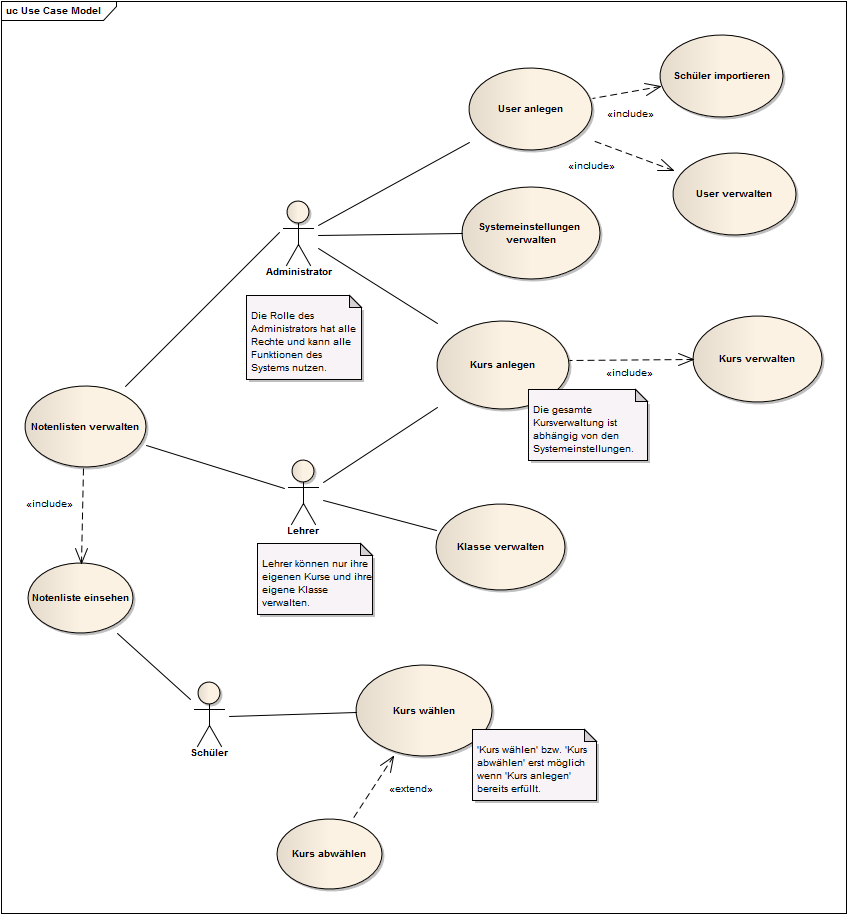
\includegraphics[scale=0.5]{img/UseCaseModel_kuwasys20.png}
 \end{center}
 \caption[\textbf{Use Case Diagram: Rollensystem}]{Use Case Diagramm: Rollensystem}
 \label{fig:UML_UC_kuwasys20}
\end{figure}

'Ein \ac{UC} beschreibt die Funktionalität des Softwaresystems, die ein Akteur ausführen muss, um ein gewünschtes Ergebnis zu erhalten oder um ein Ziel zu erreichen. \ac{UC}s sollen es ermöglichen, mit dem zukünftigen Benutzer über die Funktionalität des Softwaresystems zu sprechen, ohne sich gleich in Details zu verlieren.' Ein Zitat von \iz{Heide Balzert}{Informatikerin, die sich vor allem mit Fragen zum Thema Softwareengineering und -design beschäftigt. Derzeit ist sie Dozentin an der Fachhochschule Dortmund.}, entnommen aus \cite{BalzertH-UML2} auf Seite 28, welches den Sinn und Zweck eines \ac{UC-Diagramm}s präzise auf den Punkt bringt.

Zusammenfassend bedeutet dies, dass ein \ac{UC-Diagramm} immer dann sinnvoll ist wenn die Interaktionsmöglichkeit eines Systems, basierend auf verschiedene Aktueren, aufgezeigt werden soll. Die Akteure (dargestellt als 'Strichmännchen') im Diagramm, entsprechen genau denen, die später vom Rollensystem unterstützt werden sollen. Die Ellipsen zeigen die verschiedenen Anwendungsfälle die im System existieren. In einem so allgemeinen \ac{UC-Diagramm} wird absichtlich auf kleinste Details verzichtet. So bedeutet zum Beispiel der \ac{UC} 'Klasse verwalten' sowohl das Bearbeiten einer Klasse als auch das Vergeben von Noten oder andere klassenadministrative Aufwendungen.

Die gestrichelten Pfeile mit der Beschriftung '\texttt{$<<$include$>>$}' bezeichnen Anwendungsfälle in denen der \ac{UC}, auf welchen der Pfeil zeigt, implizit vorhanden ist wenn der \ac{UC}, von dem der Pfeil ausgeht, im System vorhanden ist. Das bedeutet wenn der \ac{UC} 'User anlegen' also vorhanden ist, auch die \ac{UC}s 'Schüler importieren' oder 'User verwalten' verwendet werden können. Ein erster \ac{UC} muss also immer erfolgen während ein zweiter (oder noch mehr) optional ausgeführt werden können.

Im Gegensatz hierzu bedeutet der gestrichelte Pfeil mit der Beschriftung '\texttt{$<<$extend$>>$}' von dem der Pfeil ausgeht, dass dieser \ac{UC} nur dann im System überhaupt vorhanden ist, wenn der \ac{UC} auf welchen der Pfeil zeigt im System vorhanden ist. Der \ac{UC} 'Kurs abwählen' ist also nur dann vorhanden wenn der \ac{UC} 'Kurs wählen' im System ausgeführt wurde. Der erste \ac{UC} wird durch den zweiten also erweitert.

\subsubsection{Statisches Analysemodell}

Im nächsten Schritt unserer Modellierung ist das statische Analysemodell, unter \prettyref{fig:UML_SA_kuwasys20} zu sehen, entworfen worden. Es stellt erste Überlegungen der Softwarearchitektur, mit konkreten Objekten inklusiver ihrer Attribute, dar und bildet ebenfalls die Beziehungen von Objekten zueinander ab. Genau genommen handelt es sich hierbei um ein 'abgespecktes' Klassendiagramm, in welchem die grobe Softwarestruktur erkennbar sein soll.

Die rechteckigen Formen stellen Klassen dar, die oben als Beschriftung ihren Namen tragen, unten die Attribute die zu ihr gehören. Die einfachen Linien sind Assoziationen zwischen den Klassen und können als Beziehungen interpretiert werden. Sie tragen einen Rollennamen und eine Multiplizität, um nachvollziehen zu können um wieviele Objekte einer Klasse es sich später mindestens und maximal handelt.
Die Rechtecke mit der Beschriftung \texttt{$<<$dataType$>>$ + String} stellen selbstdefinierte Datentypen dar.
Die Besonderheit in diesem Diagramm ist die Komposition (Assoziation mit einseitg schwarzer Raute). Sie sagt aus dass die Beziehung zwischen zwei Klassen einer starke Form der Aggregation entspricht. Die Teilklasse (Notenliste) kann also nur bestehen, solange die Aggregatklasse (Kurs) auch besteht. Würde, angewendet auf dieses Beispiel, ein Kurs gelöscht werden, würde auch der dazugehörige Notenlisteneintrag gelöscht werden. (Zur Vertiefung empfiehlt sich \cite{BalzertH_UML2} Seite 18)

In unserem Projekt entstanden zum Zeitpunkt des Softwareentwurfs 3 Klassen, die später für eine Interaktion mit dem System benötigt werden. Die Klasse für die Notenübersicht und für Kurse. Die verschiedenen Rollen wurden als Unterklassen der Klasse 'User' modelliert. Einzelne Datentypen, so bspw. für Daten zur Zeiterfassung (Datum) und zur Definition einzelner konstanter Strings (Name), wie die Rollen, wurden zur Vereinfachung vorgesehen.
Die Rollennamen sowie die Multiplizitäten der Assoziationen dürften selbsterklärend sein.

% Statisches Analyse Diagramm
\begin{figure}[H]
 \begin{center}
   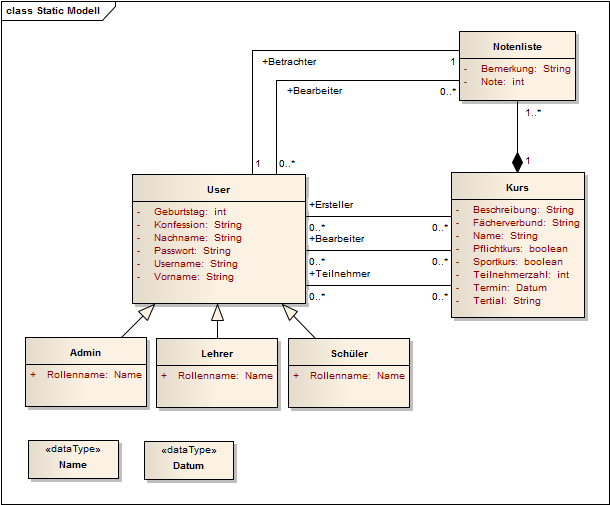
\includegraphics[scale=0.7]{img/StaticClassModel_kuwasys20.png}
 \end{center}
 \caption[\textbf{Statisches Analysemodell}]{Statisches Analysemodell}
 \label{fig:UML_SA_kuwasys20}
\end{figure}

\subsection{Benutzerschnittstellen und Rollensystem}\label{subsec:Benutzerschnittstellen und Rollensystem}

Das Kurswahlsystem der Schillerschule soll, laut Anforderungen, webbasiert mit Hilfe von verschiedenen Rollen konfiguriert und benutzt werden können.
Das System muss hierzu simultane Interaktionen, eines jeden Rollentyps, mit dem System zulassen. 

Per Aufgabendefinition liegen die vier Rollen, wie in \prettyref{subsec:Anforderungen an das System} bereits behandelt, zugrunde:

\begin{itemize}
  \item Schüler
  \item Kurslehrer
  \item Klassenlehrer
  \item Admin
\end{itemize}

Anhand der bereits vorgestellten \ac{OOM} sind, vor der Implementierung des Systems, die Rollenrechte und -richtlinien welche in den folgenden drei Unterabschnitten genaue beschrieben werden, modelliert worden.

\subsubsection{Die Rolle der Schüler}

Bei der Rolle der Schüler handelt es sich um die einfachste des Systems. 
Sie hat die wenigsten Rechte und kann hauptsächlich nur passiv, Ausnahme bildet hier die Kurswahl selbst, mit dem System interagieren.
Die Schüler welche das Kurswahlsystem erstmalig benutzen, befinden sich in der 7. Klasse. Jeder Schüler wird bis zum Abschluss der 9. Klasse das System benutzen.
Ein Schüler soll selbstständig seine Kurswahl für das jeweilige bevorstehende Tertial eines Schuljahres treffen können, dabei müssen bestimmte Abhängigkeiten eingehalten werden:

\begin{enumerate}
  \item 6 unterschiedliche Kurse pro Tertial
  \item 18 Kurse im Schuljahr
  \item 54 Kurse bis zur Vollendung des 9. Schuljahres
\end{enumerate}

\subsubsection{Die Rolle der Lehrer}

Der Rolle des Lehrers ist hingegen schon weitaus mehr Verantwortung auferlegt.
Das System unserer Webandwendung unterscheidet allerdings zwischen zwei verschiedenen Arten von Lehrern grundsätzlich nicht aufgrund einer Rollendefinition. 
Die Befugnis eines Lehrers sind lediglich abhängig von Werten die in der \ac{DB} gespeichert werden. 
Ein Klassenlehrer wird nur dann ein Klassenlehrer wenn für ihn eine Abhängigkeit zu einer Klasse besteht. 
Erst dann kann er die Funktionen, die einenm Klassenlehrer zu Verfügung stehen, nutzen.
Ein Klassenlehrer muss auf die ihm zugerordnete Klasse zugreifen und alle Kurse eines jeden Schülers einsehen können.

Das gleiche Prinzip gilt für Kurslehrer. 
Beim anlegen eines Kurses (eine Funktion die jedem Lehrer generell zur Verfügung steht) wird dieser Kurs dem Lehrer fest zugeordnet und wird somit zum Mitverantwortlichen der Kursverwaltung. 
Der Kurslehrer muss ebenfalls die Schüller einsehen können die sich in seinem Kurs befinden. Allerdings kann er nur ein Protokoll und eine Notenliste für Schüler in seinem Kurs führen.

In Abhängigkeit zur administrativen Systemverwaltung, auf die im nächsten Teil-Block eingegangen wird, hat der Lehrer nun die Rechte seine Kurse zu verwalten.

Zur Vereinfachung der Handhabung des Systems ist bereits an diesem Punkt der Modellierung an ein internes Protokollierungssystem gedacht worden. 
Es soll später die Kommunikation von Kurslehrern mit Klassenlehrern sowie die Kommunikation von Lehrern mit Schülern vereinfachen.
Im Rahmen unserer Projektarbeit wurde allerdings eine solche Funktionalität im System nicht implementiert.

\subsubsection{Die administrative Rolle des Systems}

Die administrativen Rechte des kompletten Systems stehen selbstverständlich nur dem Administrator zur Verfügung. Die Hauptaufgabe dieser Rolle im System ist es neue User ins System aufzunhemen und diese gegebenfalls zu Bearbeiten.
Das gilt für das Hinzufügen und Bearbeiten von Schülern und Lehrern gleichermaßen, beide Rollen haben also nicht die Möglichkeit sich selbst zu Verwalten.

Darüber hinaus verwaltet der Admin den Status des Systems, das aktuelle Schuljar und die dazughörigen Tertiale. Außerdem ist er der Hauptverantwortliche der Kursverwaltung.
Bevor ein Kurs stattfinden kann muss der Admin den Kurs aktivieren und für die Kurswahl zulassen. Eventuell müssen von ihm bestimmte Attribute eines Kurs noch angepasst werden können.
Ein Admin kann außerdem Fächerverbünde erstellen, bearbeiten und erstellte Kurse einem Fächerverbund zuordnen.

\subsubsection{Funktionalität des Systems}

Die Einteilung eines kompletten Schuljahrs geschieht jeweils in Tertiale. Dies kann grafisch in \prettyref{fig:Schuljahreinteilung} nachvollzogen werden. 

%%
% Schuljahreinteilung
\begin{figure}[h]
\begin{center}

\begin{tikzpicture}
    \node[draw=black, fill=yellow!20!] at (-2.5,5) {Unterteilung des Schuljahrs};
    \pie{33.3/Tertial 1, 33.3/Tertial 2, 33.3/Tertial 3}
\end{tikzpicture}

\end{center}
\caption[\textbf{Einteilung des Schuljahrs}]{Einteilung des Schuljahrs}
\label{fig:Schuljahreinteilung}
\end{figure}

Es war also nötig im administrativen Bereich des Systems eine Funktionalität vorzusehen, die es dem Admin ermöglicht das Schuljahr 'weiterzuschieben' und das entsprechende Tertial zu zu aktivieren.
Diese Verwaltungstätigkeit ist unumgänglich mit der Kurswahl verknüpft und muss für jede neu angepasst werden. 
Entscheidungen die hier während der Modellierung getroffen wurden, wurden im Hinblick auf eine möglichst einfaches \ac{UI} getroffen.

Jeder Kurs, der gewählt werden kann, gehört einem übergeordnetem Fächerverbund an, wie in \prettyref{fig:KursFaecherverbund} zu sehen ist.
Allerdings gibt es noch weitere Eigenschaften die Kurse erfüllen können. Ein Kurs kann ein Religionskurs sein, welcher für eine bestimmte Konfession ausgerichtet ist oder ein Sportkurs.
Ferner müssen Kurse als Pflichtkurse signifiziert werden können.
Aufgrund der Fülle an Informationen die verarbeitet werden müssen, war es in der Phase der Modellierung ebenfalls sehr wichtig die Datenstrukturen und deren Abhängigkeiten möglichst einfach zu halten, um in der späteren Implementierungsphase eine unkomplizierte Benutzerschnittstelle entwicklen zu können. 

%%
% Kurs - Fächerverbund
\begin{figure}[h]
\begin{center}

\begin{tikzpicture}
    \node[draw=black, fill=yellow!20!] at (-2.5,5) {Unterteilung des Schuljahrs};
    \pie{33.3/Tertial 1, 33.3/Tertial 2, 33.3/Tertial 3}
\end{tikzpicture}

\end{center}
\caption[\textbf{Einteilung des Schuljahrs}]{Einteilung des Schuljahrs}
\label{fig:KursFaecherverbund}
\end{figure}

%%
\todo[size=\small, color=green!40]{Grafik zur Abhängigkeit von Fächerverbünden bzw. Pflicht-/Sportkurse}
%%

Außer den beiden vorgestellten Datenverarbeitungen existieren selbstverständlich noch weitere, die vor allem im Sinne der Übersichtlichkeit des System  zum Tragen kommen. 
Dabei handelt es sich allerdings um Daten, die dynamisch während der Laufzeit erzeugt werden und deshalb ebenfalls in \prettyref{subsec:Systemrelevante Daten} genauer besprochen werden.
Im Gegensatz zu den dynamisch generierten Daten während der Laufzeit des Systems ist für alle anderen Daten zur Informationsverarbeitung eine Speicherung in einer Datenbank unabdingbar.
Im folgenden Unterabschnitt soll deshalb näher auf die Modellierung und Umsetzung des verwendeten Informationssystems eingegangen werden.

\subsection{Datenbankmodellierung}\label{subsec:Datenbankmodellierung}

Für die \ac{DB}-Modellierung wurde als erstes ein \ac{ER-Modell} skizziert, welches die Abhängigkeiten und Beziehungen zueinander verdeutlichen soll. Dieses ist in \prettyref{subsec:ERModell} abgebildet. Anschließend wurde das gesamte \ac{ER-Modell} in ein relationales Modell transformiert.
Mit dem entstandenen Relationalen Modell, welche in \prettyref{subsec:RelModell} dokumentiert ist, konnte anschließend auf dem Server die \ac{DB} inklusive der nötigen Tabellen erstellt werden.

\subsubsection{Entity-Relationship Modell}\label{subsec:ERModell}

Die \prettyref{fig:ERModell} zeigt das oben erwähnte \ac{ER-Modell} nach \iz{Peter Pin-Shan Chen}{Informatiker, der 1976 das ER-Modell entwickelte. Er gilt heute als Pioneer der \ac{OOM}.}, nachzulesen unter \cite{ChenPe} Seite 3 ff. bzw. \cite{VossenG-DDD} ab Seite 60.

\textbf{Aufbau des \ac{ER-Modell}s:}

Bei den blauen Rechtecken handelt es sich in diesem Modell um sogenannte Entities (Entity-Typen), die sind Dinge die in der \ac{DB} als solche abgebildet werden sollen. Sie stellen eine eigene Tabelle dar. Die gelben Ellipsen die diese umgeben, sind die Attribute (Attribut-Typen) der Entities, sie veranschaulichen die Daten welche Entities enthalten (können).
Die roten Rauten bezeichnen Beziehungen (Beziehungs-Typen) die zwischen Entities herrschen.

Das grüne Rechteck ist ein Spezialfall des 'Kurs'-Entities. Es wird als eigene Tabelle in der \ac{DB} dargestellt, ist im weitesten Sinne allerdings einer Aversion des 'Konfessions'-Attribut des 'Kurs'-Entities. Denkt man in diesem Fall an die \ac{UML}, so wäre an dieser Stelle wohl eine 'Enumeration' als eigener Datentype in Frage gekommen (Vrgl. \cite{BalzertH_UML2} Seite 10 und 11).

\tikzstyle{every entity} = [top color=white, bottom color=blue!30, draw=blue!50!black!100, drop shadow]
\tikzstyle{every weak entity} = [drop shadow={shadow xshift=.7ex, shadow yshift=-.7ex}]
\tikzstyle{every attribute} = [top color=white, bottom color=yellow!20, draw=yellow, node distance=1cm, drop shadow]
\tikzstyle{every relationship} = [top color=white, bottom color=red!20, draw=red!50!black!100, drop shadow]
\tikzstyle{every isa} = [top color=white, bottom color=green!20, draw=green!50!black!100, drop shadow]
\begin{center}
\begin{figure}[H]

\scalebox{.7}{
\begin{tikzpicture}[node distance=1.5cm, every edge/.style={link}]

%% USER
\node[entity] (usr) {Users};
\node[attribute] (usrvname) [above=2.5cm of usr] {VName} edge (usr);
\node[attribute] (usrnname) [above right=3cm of usr] {NName} edge (usr);
\node[attribute] (geb) [above left=3cm of usr] {Geburtsdatum} edge (usr);
\node[attribute] (usrkonf) [above left=of usr] {Konfession} edge (usr);
\node[attribute] (usrklasse) [above=of usr] {Klasse} edge (usr);
\node[attribute] (usrusername) [above right=of usr] {\key{Username}} edge (usr);
\node[attribute] (usrpassword) [right=of usr] {Passwort} edge (usr);
\node[attribute] (usrid) [below=0.3cm of usr] {\key{UserID}} edge (usr);

%% REL "hat"
\node[relationship] (hat) [left=1.5cm of usr] {hat} edge (usr);

%% REL "eingetragen"
\node[relationship] (eingetragen) [below left =3cm of usr] {eingetragen} edge (usr);
%
%% ROLLE
\node[entity] (rolle) [left=1cm of hat] {Rolle} edge (hat);
\node[attribute] (rollename) [left=of rolle] {\key{Username}} edge (rolle);
\node[attribute] (rolleusrnname) [above left=of rolle] {Rolle} edge (rolle);

%% REL "besucht"
\node[relationship] (besucht) [below right=of usr] {besucht} edge (usr);

%% KURS
\node[entity] (kurs) [below right=1cm of besucht] {Kurs} edge (besucht);
\node[entity, top color=white, bottom color=green!30, draw=green!50!black!100, drop shadow] (kurskonf) [above=1.5cm of kurs] {Kurskonfession} edge (kurs);
\node[attribute] (termin) [above right =.2cm of kurskonf] {Termin} edge (kurs);
\node[attribute] (kursl) [right =.2cm of kurskonf] {Kurslehrer} edge (kurs);
\node[attribute] (teilm) [above right=0.2cm of kurs] {Teilnehmerzahl} edge (kurs);
\node[attribute] (kursid) [left=0.2cm of kurs] {\key{KursID}} edge (kurs);
\node[attribute] (faecher) [right=0.2cm of kurs] {Fächerverbund} edge (kurs);
\node[attribute] (flags) [below=2.5cm of kurs] {Sportkurs} edge (kurs);
\node[attribute] (flag3) [below=2.2cm of faecher] {Pflicht} edge (kurs);
\node[attribute] (tertial) [below left=.2cm of flag3] {Tertial} edge (kurs);
\node[attribute] (flag2) [below=1.2cm of faecher] {Konfession} edge (kurs);
\node[attribute] (bemerk) [below=of kurs] {Beschreibung} edge (kurs);
\node[attribute] (kursname) [below right=0.2cm of kurs] {Kursname} edge (kurs);

%% REL "enthält"
\node[relationship] (enthalten) [below left =of kurs] {enthalten} edge (kurs);

%% NOTENLISTE
\node[entity] (notenliste) [below right=2cm of eingetragen] {Notenliste} edge (enthalten) edge (eingetragen);
\node[attribute] (note) [below left=1cm of notenliste] {Note} edge (notenliste);
\node[attribute] (usrkonf) [above =of notenliste] {Bemerkung} edge (notenliste);
\node[attribute] (usrvname) [below=of notenliste] {\key{KursID}} edge (notenliste);
\node[attribute] (usrnname) [left=of notenliste] {\key{UserID}} edge (notenliste);
\node[attribute] (listid) [below right=1.2cm of notenliste] {\key{ListenID}} edge (notenliste);

%% SYSTEM
\node[entity] (system) [below=5cm of notenliste] {System};
\node[attribute] (schuljahr) [below=of system] {Schuljahr} edge (system);
\node[attribute] (tertial) [left=of system] {Tertial} edge (system);
\node[attribute] (wochd) [below left= of system] {Phase} edge (system);
\end{tikzpicture}
}
\caption[\textbf{Entity-Relationship Modell}]{Entity-Relationship Modell}
\label{fig:ERModell}
\end{figure}
\end{center}

\textbf{Interpretation des \ac{ER-Modell}s:}

Um die Interpretation, also den Gedankengang der \ac{DB}-Modellierung, zu verdeutlichen macht es Sinn, die Beziehungen genau auszuformulieren.
Dabei werden alle Beziehungen zu jedem Entity betrachtet, begonnen mit dem Entity.
Zusätzlich sollen die Multiplizitäten mit einfließen, um die Abhängigkeiten zu verdeutlichen und um die Transformation in ein Datenbankmodell zu erleichtern.

Die Schreibweise dieser Multiplizitäten ist wie folgt definiert:

Sei $E_{A}$ das erste und $E_{B}$ das zweite Entity.
Die Beziehung beider Entities ist definiert als $R_{AB}$. 
Die erste Multipliziät $(0,N)$ gibt Auskunft über die Häufigkeit von $E_{A}$ in der geltenden Beziehung zu $E_{B}$.
Die zweite $(1;M)$ über die Häufigkeit von $E_{B}$ zu $E_{A}$.

Man kann also schreiben:

\begin{center}
$E_{A}$ ist $(0;N)$ in Beziehung $R_{AB}$ zu $E_{B}$

oder

$E_{B}$ ist $(1;M)$ in Beziehung $R_{AB}$ zu $E_{A}$
\end{center}

Wobei die erste Zahl bei der Angabe der Multiplizität, also die vor dem Semikolon (';') für die minimalste, die zweite Zahl für die maximalste Gültigkeit unter der bestendenen Bedingung steht.

Begonnen werden soll die genauere Betrachtungsweise mit dem Entity 'User':

\begin{enumerate}
  \item User - Rolle (beidseitig):	
    \begin{itemize}
      \item einem User ist genau $(1;1)$ Rolle zugeteilt
      \item einer Rolle hingegen können $(0;N)$ User zugeteilt sein
    \end{itemize}

  \item User - Kurs
    \begin{itemize}
      \item ein Schüler wählt $(0;N)$ viele Kurse
      \item ein Lehrer erstellt/verwaltet $(0;M)$ viele Kurse
    \end{itemize}
  
  \item User - Notenliste:
    \begin{itemize}
      \item ein Schüler hat $(1;1)$ Eintrag in der Notenliste für jeweils einen fest zugeordneten Kurs (Vrgl. Kurs - Notenliste)
    \end{itemize}

\end{enumerate}

Konkretisieren wir nun das Entity 'Kurs':

\begin{enumerate}
  \item Kurs - Notenliste:
  \begin{itemize}
    \item ein Kurs besitzt genau $(1;1)$ Eintrag pro Kurs in der Notenliste für einen Schüler (Vrgl. User - Notenliste)
  \end{itemize}
  
  \item Kurs - Kurskonfession	
    \begin{itemize}
      \item ein Kurs hat genau $(0;1)$ Konfessionszugehörigkeit
    \end{itemize}

  \item Kurs - User	
    \begin{itemize}
      \item ein Kurs wird von $(0;N)$ vielen Schülern gewählt
      \item ein Kurs wird immer genau $(1;1)$ Lehrern zugeteilt
    \end{itemize}
\end{enumerate}

Für das letzte Entity der Dreier-Beziehung 'Notenliste' gelten lediglich die bereits beschriebenen Abhängigkeiten und Beziehungsverhältnisse. 
Zur Verdeutlichung sollen diese jedoch nochmals aufgeführt werden.

\begin{enumerate}
  \item Notenliste - User:
  \begin{itemize}
    \item eine Notenliste hat im Bezug auf genau einen Kurs $(0;N)$ Einträge für einen User
  \end{itemize}
  
  \item Notenliste - Kurs:
  \begin{itemize}
    \item Ein Schüler wählt $(1;N)$ viele Kurse, ein Kurs wird von $(1;N)$ vielen Schülern besucht/gewählt.
  \end{itemize}
  
\end{enumerate}

Das Entity 'System' besitzt keine Beziehungen innerhalb der Datenbank, weshalb auf eine ausführliche Interpretation verzichtet werden kann.
Die Darstellung dieses Entities wird innerhalb der \ac{DB} sowieso über eine eigene Tabelle umgesetzt.

Der nächste Schritt ist nun die Transformation von \ac{ER-Modell} in das Relationale \ac{DB}-Modell.

\subsubsection{Relationales Modell}\label{subsec:RelModell}

Bei der Beschreibung des Relationalen Modells der KuWaSys-\ac{DB} ist das Hauptaugenmerk auf die komplette Datenverarbeitung gelegt, also vor allem auch Implementierungen für Vorgänge die für den Benutzer des Systems nicht unmittelbar zu sehen sind.
Daten die für die Oberfläche und die einzelnen Benutzerschnittstellen eine tragende Rolle spielen sollen unter (Abschnitt Benutzerschnittstellen) gesondert behandelt werden und werden im Laufe dieses Kapitels nur kurz angesprochen.

Die Vorüberlegungen zur Transformation von mehrwertigen Attributen von Entities sind bereits abgeschlossen.
Prinzipiell kann man mit der Transformation, wie in \cite{VossenG-DDD} beschrieben ist wie folgt vorgehen:

\begin{enumerate}
 \item Jedes Entity wird in eine relationale Form gebracht
 \item Jeder Beziehungs-Typ ebenfalls, es sei denn:
 \begin{itemize}
  \item es handelt sich um eine zweistellige $1:1$-Beziehung
  \item es handelt sich hierbei um eine $1:N$-Beziehung
 \end{itemize}
\end{enumerate}

Die Beschreibung $1:1$- bzw $1:N$-Beziehung bedeutet in diesem Fall allerdings nicht wie zuvor, ein Minimum auf der linken und das Maximum auf der rechten Seite. 
Hierbei werden nur noch die maximalen Werte der beiden Multiplizitätsangaben berücksichtigt. Dies gilt analog für alle Angaben der Multiplizitäten.

Sollte bei der Transformation $Punkt$ $2)$ eine Rolle spielen, müssen Attribute in bereits bestehende Relationsschemata aufgenommen werden. Folgende Regeln treten dann in Kraft:
\begin{enumerate}
 \item Zweistellige $1:1$-Beziehung
 \begin{itemize}
  \item ein Entity stellt selbst ein Relationsschema dar
  \item Attribute des zweiten Entities werden ebenfalls in dieselbe Tabelle gespeichert
 \end{itemize}
 \item Zweistellige $1:N$-Beziehung
 \begin{itemize}
  \item ein Entity stellt ein eigenes Relationsschema dar
  \item erste Möglichkeit: die Attribute des Entities welches die maximale Multiplizität von $1$ aufweist wird hingegen dem Realtionsschema mit der maximalen Multiplizität von $N$ in Form von Fremdschlüsseln zugeschrieben
  \item zweite Möglichkeit: es wird ein eigenes Relationsschema für die Beziehung der beiden Entities angelegt. Dieses neu entstande Schema erhält dann Attribute, welche widerum Fremdschlüssel der beiden anderen Entities sind
 \end{itemize}
\end{enumerate}

Die Transformation vom \ac{ER-Modell} ins Relationale Modell (zur bildhaften Darstellung ist die Kopfzeile der dazugehörigen Tabelle auch gezeigt) sieht im Falle des Kurswahlsystems folgendermaßen aus:

\textbf{Users} = \{( \underline{id:serial}, nachname:character, vorname:character, geburtstag:character, konfession:character, klasse:character, \underline{username:character}, passwort:character )\}

% User-Tabelle
\begin{table}[H]
\begin{center}
	\begin{tabular}{|c|c|c|c|c|c|c|c|}\hline
		\textbf{\underline{ID}} & \textbf{NName} & \textbf{VName} & \textbf{Geb} & \textbf{Konf} & \textbf{Klasse} & \textbf{\underline{Username}} & \textbf{Passwort} \\ \hline
		\vdots & \vdots & \vdots & \vdots & \vdots & \vdots & \vdots & \vdots \\
	\end{tabular}
	\caption{Kopfzeile der User-Tabelle}
\end{center}
\end{table}

\textbf{Kurs} = \{( \underline{id:serial}, name:character, kurslehrer:integer, faecherverbund:character, termin:integer, beschreibung:character, schuljahr:integer, tertial:integer, 
teilnehmerzahl:integer, pflichtkurs:boolean, sport:boolean )\}

% Kurs-Tabelle
\begin{table}[H]
\begin{center}
	\begin{tabular}{|c|c|c|c|c|c}\hline
		\textbf{\underline{ID}} & \textbf{Name} & \textbf{Kurslehrer} & \textbf{Faecherverbund} & \textbf{Termin} & \dots \\ \hline
		\vdots & \vdots & \vdots & \vdots & \vdots & \dots \\
	\end{tabular}
	\caption{Kopfzeile der Kurs-Tabelle  (unvollständig)}
\end{center}
\end{table}

\textbf{Kurs-Konfessionen} = \{( \underline{religionid:integer}, konfession:character )\} 
 
% Kurs-Konfession-Tabelle
\begin{table}[H]
\begin{center}
	\begin{tabular}{|c|c|}\hline
		\textbf{\underline{ReligionID}} & \textbf{Konfession} \\ \hline
		\vdots & \vdots \\
	\end{tabular}
	\caption{Kopfzeile der Kurs-Konfessions-Tabelle}
\end{center}
\end{table}

\textbf{Notenliste} = \{( \underline{id:serial}, note:integer, bemerkung:character, userid:integer, kursid:integer, jahr:integer, tertial:integer )\}

% Notenliste-Tabelle
\begin{table}[H]
\begin{center}
	\begin{tabular}{|c|c|c|c|c|c|c|}\hline
		\textbf{\underline{ID}} & \textbf{Note} & \textbf{Bemerkung} & \textbf{UserID} & \textbf{KursID} & \textbf{Jahr} & \textbf{Tertial}\\ \hline
		\vdots & \vdots & \vdots & \vdots & \vdots & \vdots & \vdots  \\
	\end{tabular}
	\caption{Kopfzeile der Notenlisten-Tabelle}
\end{center}
\end{table}

\textbf{Rolle} = \{( \underline{username:character}, rolle:character )\}

% Rollen-Tabelle
\begin{table}[H]
\begin{center}
	\begin{tabular}{|c|c|}\hline
		\textbf{\underline{Username}} & \textbf{Rolle} \\ \hline
		\vdots & \vdots \\
	\end{tabular}
	\caption{Kopfzeile der Rollen-Tabelle}
\end{center}
\end{table}

\textbf{System} = \{( \underline{phase:integer}, jahr:integer, tertial:integer )\}

% System-Tabelle
\begin{table}[H]
\begin{center}
	\begin{tabular}{|c|c|c|}\hline
		\textbf{\underline{Phase}} & \textbf{Jahr} & \textbf{Tertial} \\ \hline
		\vdots & \vdots & \vdots \\
	\end{tabular}
	\caption{Kopfzeile der System-Tabelle}
\end{center}
\end{table}

\subsection{Konfiguration der Laufzeitumgebung und des Servers}\label{subsec:Konfiguration der Laufzeitumgebung und des Server}

Dieses Kapitel ist als Zwischenschritt, von der Modellierung zur Implementierung, unseres Softwareprojekts zu verstehen.
Zum Einen galt es eine komplette bestehende Infrastruktur zu überblicken und zu verstehen (dieser Schritt kann als eine Art der Modellierung verstanden werden)
zum Anderen musste ein komplettes neues System einwandfrei funktionsfähig eingebettet werden (zu vergleichen mit dem Schritt der Implementierung).

\textbf{Sichtung der bestehenden Infrastruktur:}

Die Schillerschule teilt sich mit der benachbarten Realschule am Galgenberg eine Serverinfrastruktur nach der Novell Musterlösung paedML 3.33, weitere Informationen sind unter \cite{paedML} zu finden. % VMWare ASG 220 Astaro.
Diese beinhaltet eine virtuelle Infrastruktur \gls{VMWare} ESXi auf der ein \ac{SLES} Novell Server gehostet ist.

\begin{figure}[H]
\begin{center}
\begin{tikzpicture}[
  scale=0.1,
  font=\sffamily,
  every matrix/.style={ampersand replacement=\&,column sep=2cm,row sep=2cm},
  source/.style={draw,thick,rounded corners,fill=yellow!20,inner sep=.3cm},
  process/.style={draw,thick,circle,fill=blue!20},
  sink/.style={source,fill=green!20},
  datastore/.style={draw,very thick,shape=datastore,inner sep=.3cm},
  dots/.style={gray,scale=2},
  to/.style={->,>=stealth',shorten >=1pt,semithick,font=\sffamily\footnotesize},
  every node/.style={align=center}]

  % Positionierung über Matrix-Layout
  \matrix{

    \node[source] (Ubuntu) {Ubuntu 12.04 VM\\ ($141.10.50.250$)};
      \& \node[process] (Suse) {Server}; \& \\
      \& \node[sink] (firewall) {ASG 220 Astaro\\ ($Firewall$)}; \& \\

    \node[source] (SLES) {SuSE Linux\\ Enterprise Server\\ ($SLES$)}; \& \\

    \node[datastore, color=black!50!white] (infrastructure) {Einstellungen\\($Novell$ $paedML$ $3.3$)}; \& \\


      \& \node[process] (router) {Router};
      \& \node[sink] (www) {WWW}; \\
  };

  % VM - Host
  \draw[to, very thick] (Ubuntu) -- node[midway,above] {VM Host}
      node[midway,below] {} (Suse);

  % FW - Host
  \draw[to, dashed, very  thick] (Suse) -- node[midway,above] {}
       node[midway,below] {} (firewall);itemize
  \draw[to, dashed, very  thick] (firewall) -- node[midway,above] {}
       node[midway,below] {} (Suse);

  % FW - Router
  \draw[to, very thick] (router) -- node[midway,above] {}
       node[midway,below] {} (firewall);
  \draw[to, very  thick] (firewall) -- node[midway,above] {}
       node[midway,below] {} (router);

  % Einstellungen Infrastruktur
  \draw[color=black!50!white] (infrastructure) -- node[midway,above] {}
       node[midway,below] {} (SLES);

  % SLES - Netz
  \draw[to, very thick] (SLES) -- node[midway,above=1cm] {VM Host}
       node[midway,below] {} (Suse);
  \draw[to, dashed, color=black!50!white] (SLES) -- node[midway,right=0.2cm] {Konfiguration}
       node[midway,below] {} (router);
  \draw[to, dashed, color=black!50!white] (SLES) -- node[midway,right=0.2cm] {Konfiguation}
       node[midway,below] {} (Ubuntu);

  % Router - WWW
  \draw[to, very thick] (router) -- node[midway,above] {}
       node[midway,below] {} (www);
  \draw[to, very thick] (www) -- node[midway,above] {}
       node[midway,below] {} (router);
\end{tikzpicture}
\end{center}
\caption[\textbf{Netzwerkstruktur der Schillerschule Aalen}]{Netzwerkstruktur der Schillerschule Aalen mit DMZ}
\label{fig:Netzwerkstruktur}
\end{figure}

Prinzipiell wäre eine Verwendung dieser virtuellen \gls{Appliance} zum Hosting der \ac{Webapp} möglich. Um jedoch die Systemsicherheit zu erhöhen ist eine weitere virtuelle Appliance, die nur das Kurswahlsystem bereitstellt die bessere Wahl.
\iz{Ubuntu Server 12.04 LTS}{http://www.ubuntu.com/} läuft auf diesem virtuellen Rechner, der sich wie der oben genannte SLES in der \gls{DMZ} der virtuellen Netzwerkinfrastruktur befindet.

\textbf{Integration in die Infrastruktur:}

Ein PostreSQL-Server dient zur Datenhaltung und ein Apache Tomcat 7 zur Auslieferung der \ac{Webapp}. Nach Konfiguation (und überfälligem reboot) der Astaro Firewall im Keller der Schule ist die Webapp jetzt über das Intranet an allen Rechnern im Schulnetz erreichbar (\url{http://192.168.1.222:8080/kuwasys20}). Die Erreichbarkeit über das Internet ist seit der Freischaltung der entsprechenden Ports auf den BelWü-Server und umgekehrt gegeben (\url{http://141.10.50.250:8080/kuwasys20}).
Diese Adressen werden auf der Homepage der Schillerschule und im Intranet verlinkt, sodass keine weitere Maskierung wie Subdomains oder lokale DNS-Einträge notwendig ist.
Die Admnistration des Ubuntu Servers kann im Intranet von einer VMWare Management Console aus erfolgen, für schnelles Eingreifen wurde ein \gls{Secure Shell} (SSH) Zugang eingerichtet, der im Internet erreichbar ist.

In \prettyref{fig:Netzwerkstruktur} ist die neue Struktur des Netzwerks dargestellt.

Die Einrichtung eines Backups war für unser Projekt nicht notwendig, da die Schillerschule selbst schon über ein funktionsfähiges Backupsystem verfügt. Hierbei wird in bestimmten Intervallen die komplette Festplatte des Servers gespiegelt, und somit auch die virtuellen Maschinen.
Somit ist die Garantie gegeben, dass auch das Kurswahlsystem einem ständigen Sicherungsvorgang unterliegt und im Notfall wiederhergestellt werden kann.
\newpage

\section{Implementierung}	\label{sec:Implementierung}
							\label{secmin:Implementierung}

In einem System, in welchem ein \gls{Multi-User Betrieb} möglich sein soll, ist das Design der Oberfläche und das der einzelnen Benutzerschnittstellen unweigerlich eng miteinander verknüpft. 
Es müssen in der Phase der Implementierung bereits exakte Schnittstellen definiert und strukturierte Oberflächen skizziert worden sein um spätere Korrekturen gering zu halten oder um sie zu vermeiden.

In den folgenden zwei Abschnitten sollen grundlegende Implementierungsgedanken besprochen werden, die mit den Anforderungen an das System in erster Linie nichts zu tun haben. 
Zuerst soll die Art und Weise der Umsetzung der Benutzerschnittstellen und des Designs näher erklärt werden. Danach sollen elementare Datenstrukturen die zum Einsatz kamen und in JSF implementiert wurde näher erläutert werden.

Nach den beiden einführenden Abschnitten wird dem Leser detailiert dargestellt wie die zu bewältigenden Systemanforderungen in JSF umgesetzt wurden. 
Dabei werden Quellcodeausschnitte sowie Diagramme zum Einsatz kommen die dem Leser das Verstehen erleichtern sollen.
Da während allen Phasen der Umsetzung des Projekts auch immer die Modularität des gesamten Systems im Vordergrund stand soll hier nicht kleinlichst genau erklärt werden was im Quellcode steht, sondern darauf eingegangen werden, wie das zu lösende Problem angegangen wurde und schlussendlich welche wichtigen Bausteine zu tragen kamen. 
An dieser Stelle soll außerdem nochmals die Wichtigkeit der oben besprochenen Datenbankmodellierung erwähnt werden. Gründe für die verschiedenen Umsetzungen der Modellierung sollen im Abschnitt der Implementierung dieser Ausarbeitung nicht mehr näher besprochen werden. 
Es wurde jedoch viel Wert darauf gelegt die Schritte der Implementierung gut und verständlich zu formulieren und darzustellen.

\subsection{Benutzerschnittstellen und Oberflächendesign}

Wir haben uns für ein simples und einfach zu verstehendes Oberflächendesign entschieden, welches allerdings den Design Aspekten der \gls{Corporate Identity} (CI) erfüllen sollte. 
%%
\todo[size=\small, color=green!40]{HMI Buch Zitate etc...}
%%
Im allgemeinen wird beim Screendesign bestimmten Regeln gefolgt, welche durch das gewählte Gestaltungsraster festgelegt werden.

Hierzu wurden von uns folgende Bereiche festgelegt:
\begin{itemize}
  \item Kopf- oder Bannerbereich mit Logo
  \item Navigationsbereich bzw. Unternavigation
  \item Arbeitsbereich
  \item Impressum/Hinweise
\end{itemize}

Der Hauptaufbau dieser Seiten, auf welche im folgenden näher eingegangen wird, wurden mit Templates, wie es bereits in \prettyref{subsec:Darstellung von Seiteninhalten} angesprochen wurde, umgesetzt.
Der allgemeine Aufbau soll im folgenden besprochen werden, der nachstehende Quellcodeausschnitt zeigt einen Teil des Templates das von uns zur Gestaltung der Seiten verwendet wurde:

% LISTING
% template.xhtml 
%%
\todo[size=\small, color=red!40]{Listing}
%%
Auffallend ist vor allem der Kopf der Seite, welcher den Wiedererkennungswert (Vrgl. hierzu die \iz{Webiste der Schillerschule}{\url{http://www.schillerschule-aalen.de}}) ganu im Sinne des \ac{CI}s steigern soll.
Hierzu wurde die Grafik lediglich transparenter gehalten als ihr Original und hat ganz im Stil der Schule die Überschrift erhalten wie in \prettyref{fig:header_KuWaSys} zu sehen ist.

% Header
\begin{figure}[H]
 \begin{center}
   
\includegraphics[scale=0.4]{img/header_KuWaSys.png}
 \end{center}
 \caption[\textbf{KuWaSys: Banner des Systems (Header)}]{KuWaSys: Banner des Systems (Header)}
 \label{fig:header_KuWaSys}
\end{figure}

Die Navigation und deren Unternavigationspunkte sind im linken Bereich der Webiste angeordnet und unterstützen den User visuell mit Hervorhebungen, wie in \prettyref{fig:navihervorhebung_KuWaSys} dargestellt ist, bei der Arbeit mit dem System.
Nötige Unternavigationspunkte, falls diese vorhanden sind, öffnen sich automatisch beim Klick auf ein übergeordnetes Menüelement, sodass die komplette Menüstruktur handlich und kompakt dargestellt erscheint und mit einem Blick erfasst werden kann.

Der Arbeitsbereich wird in der Mitte der Seite dargestellt, unterhalb des Kopfbereichs und rechts der Navigation. 
Dieser wird abgetrennt durch blaue Balken (links zur Navigation sowie oben zum Kopfbereich) um die Einteilung der Seite für die Benutzer des Systems eindeutig und übersichtlich zu halten.
Jede Interaktion mit dem System wird in diesem Bereich der Website dargestellt. 
%%
\todo[size=\small, color=green!40]{Grafik zu Bildschirmenteilung}
%%

% Infobar
\begin{figure}[h]
 \begin{center}
   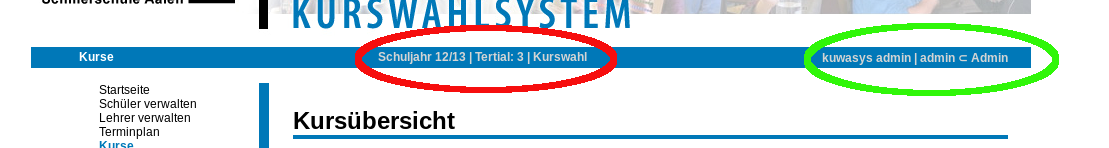
\includegraphics[scale=0.4]{img/informationbar_KuWaSys.png}
 \end{center}
 \caption[\textbf{KuWaSys: Informationsbalken (oberer Bereich)}]{KuWaSys: Informationsbalken (oberer Bereich)}
 \label{fig:infobar_KuWaSys}
\end{figure}

Zur erwähnen ist zudem noch der Trennbalken nach oben welcher zusätzlich als Informationsanzeige für den User verwendet wird und der Fußbereich welcher Informationen zur Website enthält. 
Die obere Anzeige, hier werden Informationen zum User selbst (Voller Name, Username und Rolle im System) und Informationen zum aktuellen Status des Systems (aktuelles Schuljahr und aktuelles Tertial) angezeigt.
Die \prettyref{fig:infobar_KuWaSys} zeigt die genaue Einteilung des Infobalkens oben, rot die Informationen des Systems, grün die Informationen des Users.
Der Fußbereich dient ausschließlich zur weiteren Information beim Besuch der Webiste welcher in \prettyref{fig:footer_KuWaSys} zu sehen ist.  

Die Hauptfarben des Systems wurden absichtlich blau gewählt um eine gewisse Professionalität sowie Seriösität gegenüber den Benutzern auszustrahlen. Diese ziehen sich kontinuierlich durch das gesamte System

%%
\todo[size=\small, color=green!40]{HMI Buch Dahm...}
%%

% Navibar
\begin{wrapfigure}[18]{r}{12cm}
 \begin{center}
   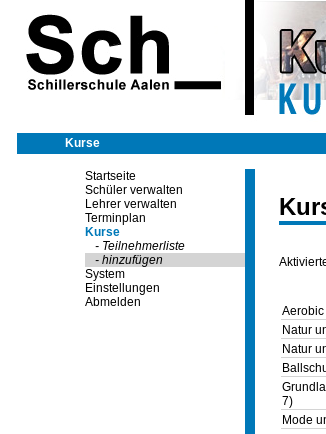
\includegraphics[scale=0.65]{img/navigation_KuWaSys.png}
 \end{center}
 \caption[\textbf{KuWaSys: Navigations und Menüelemente (linker Bereich)}]{KuWaSys: Navigations und Menüelemente (linker Bereich)}
 \label{fig:navihervorhebung_KuWaSys}
\end{wrapfigure}

Auf ein Impressum oder auf rechtliche Hinweise konnte bei dieser Art von Webiste verzichtet werden. 
Erstens handelt es sich hierbei um keine kommerzielle Website, laut \textit{§5} \ac{TMG} wird ein Impressum von 'geschäftsmäßigen Online-Diensten' benötigt, 
%%
\todo[size=\small, color=green!40]{rechtlicher Nachweis} zweitens um keine öffentliche oder frei zugängliche Website, 
%%
wobei hier die Vorschrift des \textit{§55} \ac{RstV} besagt, dass eine Impressumspflicht nur dann besteht wenn der Inhalt der Website regelmäßig journalistisch-redaktionelle Inhalte online zur Verfügung stellt.
(Gesetzesauszüge sind im Anhang unter \prettyref{subsec:Gesetz} zu finden) 

% Footer
\begin{figure}[h]
 \begin{center}
   \includegraphics[scale=0.7]{img/footer_KuWaSys.png}
 \end{center}
 \caption[\textbf{KuWaSys: Informationsbalken (unterer Bereich)}]{KuWaSys: Informationsbalken (unterer Bereich)}
 \label{fig:footer_KuWaSys}
\end{figure}

Zur Strukturierung von Seiteninhalten wurden herkömmliche \ac{JSF}-Standardkomponenten verwendet.
Zu den hauptsächlich verwendeten, zählen:
\begin{itemize}
  \item \texttt{<h:outputText>}\\
    Element welches HTML-Text auf der Obefläche ausgibt 
  
  \item \texttt{<h:outputLabel>}\\
    auch normaler Text, allerdings als Beschriftung von Texteingabefeldern
      
  \item \texttt{<h:inputText>}\\
    Element zur Texteingabe, Synonyme für ein HTML \texttt{<input>}-Tag mit type="text"
  
  \item \texttt{<h:inputSecret>}\\
    Element zur verschlüsselten Texteingabe, entspricht \texttt{<input>}-Tag mit type="password"
  
  \item \texttt{<h:commandButton>}\\
    Button in HTML, der Klick löst eine definierte Aktion über eine ManagedBean-Methode aus

  \item \texttt{<h:panelGrid>}\\
    Darstellung einer Tabelle, Synonym für das HTML \texttt{<table>}-Tag. Die Anzahl der Spalten wird über das \texttt{columns}-Attribut festgelegt
  
  \item \texttt{<h:panelGroup>}\\
    Container-Element (mehrere JSF-Tags werden zu einem zusammenfügt)
  
  \item \texttt{<h:message>}\\
    gibt eine Fehlermeldung für die definierte Komponenten aus (\texttt{ErrorStyle}-Attribut über \ac{CSS} steuerbar)
  
  \item \texttt{<h:form>}\\
    stellt ein Formular dar, welches einen POST-Request per HTTP absetzt
  
  \item \texttt{<f:facet>}\\
    Definiert eine Facette (bspw. die Überschrift für eine Tabelle)
\end{itemize}

Außer den eben erwähnten Komponenten gibt es eine Vielzahl anderer bis hin zu selbstdefinierten welche im entwickelten System zum Einsatz kommen. Diese werden allerdings nicht näher betrachtet, da sie für das umgesetzte System irrelevant sind. Selbstverständlich kann zur grafischen Darstellung auch normale \ac{HTML}-Syntax verwendet werden.
Um die Strukturierung des Seitenaufbaus übersichtlich zu halten wird ebenfalls das wohl bereits bekannte Grundlagenwerkezug der Webentwicklung, die \gls{Cascading Style Sheets} (CSS), für die Eigenschaften der Darstellungselemente, eingesetzt.
Vorteile dieser Vorgehensweise der Datenverarbeitung resultiert in einer einheitlichen und damit gut strukturierten Darstellung der betroffenen Websites.

%%
\todo[size=\small, color=green!40]{CSS/Komponenten Listings}
%%

\subsection{Informationsdarstellung und -verarbeitung}

Eine elementare Datenstrukturen im System sind Listen, welche dem User in Form einer Tabelle dargestellt werden.
Die Vorteile dieser Datenstruktur sind die Einfachheit der Datenhaltung sowie der Zugriff auf die Daten und Bereitstellung dieser.

Grundlegend sind zwei zu unterscheidende Listen im System implementiert:
\begin{enumerate}
  \item User-Listen (Schüler und Lehrer)
  \item Kurs-Listen
  \item Noten-Listen
\end{enumerate}

Dabei sind beide Listen lediglich nach Art des Inhalts ihrer Daten zu differenzieren. Die für die Benutzeroberfläche relevanten sollen kurz erläutert werden:

\textbf{Schüler}
\begin{itemize}
  \item ID: Integer, welcher für das Wählen von Kursen und das Vergeben von Noten wichtig ist, da diese einen Fremdschlüssel in der jeweiligen Tabelle darstellt
  \item Vorname und Nachname: String, der den realen Namen des Users wiedergibt
  \item Klasse: String, zur Identifizierung welchem Klassenlehrer ein Schüler zugeordnet ist, bzw wie weit er in seiner Schullaufbahn vorangeschritten ist
  \item Konfession: String, zur Identifizierung des Religionsunterrichts der angeboten werden kann bzw. muss während dem Erstellen eines Kurses. (Näheres in Abschnitt Kurswahl)
\end{itemize}

\textbf{Lehrer}
\begin{itemize}
  \item ID (mit der gleichen Bedeutung wie bei Schülern)
  \item Vorname und Nachname (ebenfalls gleich wie bei Schülern)
  \item Klasse: String, der festlegt, von welcher Klasse ein Lehrer Klassenlehrer ist
\end{itemize}

\textbf{Kurse}
\begin{itemize}
  \item Kursnummer
  \item Kursname
  \item Kursbeschreibung
  \item Teilnehmeranzahl
\end{itemize}

\textbf{Notenlisten}
\begin{itemize}
  \item Schülername
  \item Kursname
  \item Note
  \item Bemerkung
\end{itemize}

Die Implementierung der Listen in Java wurde über Listen vom Typ \texttt{ArrayList<List>} umgesetzt. 
%%
\todo[size=\small, color=orange!40]{technische Umsetzung von Listen, Grundlagen etc... am Beispiel von Java Listings - 1 bis 2 Getter/Setter}
%%
%%
\todo[size=\small, color=orange!40]{dazugehöriges Facelet, bpw. Schüler}
%%
%%
\todo[size=\small, color=orange!40]{Datenbankabfrage und 'Befüllen' der Listen}
%%


\subsection{Benutzerauthentifizierung}

Einer der elementarsten Vorgänge im System ist der Login-Vorgang. Es handelt sich hierbei um einen Vorgang den jeder Benutzer egal mit welcher Rolle vor der Interkation mit dem System durchlaufen muss. Zur Verifizierung eines Users am System wird sein Kürzel, welches beim Anlegen automatisch aus Vor- und Nachnamen generiert wird, sowie ein Passwort, welches ebenfalls automatisch und randomisiert generiert wird, benötigt. Die Anmeldemaske, welche zugleich auch die Startseite des Kurswahlsystems bildet, kann in \prettyref{fig:login_KuWaSys} angesehen werden. Die Registrierung eines Users am System kann ausschließlich durch den Admin erfolgen.

% Login
\begin{wrapfigure}[12]{l}{10cm}
 \begin{center}
   \includegraphics[scale=0.7]{img/login_KuWaSys.png}
 \end{center}
 \caption[\textbf{KuWaSys: Login Maske und Startseite}]{KuWaSys: Login Maske und Startseite}
 \label{fig:login_KuWaSys}
\end{wrapfigure}


Für den Vorgang des Logins am System besitzt der Servlet-Container Tomcat 7 eine sehr hilfreiche und gängige Funktion der Softwareentwicklung, die Konfiguation des \ac{DBCP}s des Apache Commons Projekts. Nähere Informationen sind unter \cite{ApacheDBCP} zu finden. 

Wie bereits aus dem \prettyref{subsec:Datenbankmodellierung} bekannt ist, haben wir für unser Datenbank eine zusätzliche Tabelle 'Rolle', die mit der Tabelle 'User' in Relation steht, modelliert. Diese wird nun für die Konfiguration des \ac{DBCP}s benötigt.

Der \ac{DBCP} gehört zu einer Art

Aufgrund der Tatsache, dass die Rollen-Tabelle mit der User-Tabelle in einer Beziehung zueinander steht, kann bei der Authentifizierung also genau auf den gewollten User zugegriffen werden. Diese Tatsache machen wir uns auch im weiteren Verlauf der Systemimplementierung zu Nutze, bspw. bei der Generierung von Benutzerdaten (\prettyref{subsec:Daten eines Benutzers}) oder aber um Daten zu manipulieren die mit dem User in Verbindung stehen.

%%
\todo[size=\small, color=orange!40]{Datenbankabfrage und Check Methoden Listing}
%%
 

\subsection{Benutzerverwaltung}\label{subsec:Daten eines Benutzers}
%%
\todo[size=\small, color=red!40]{Eindeutigkeit von Usernamen/Passwort bei Generierung}
%%

\subsubsection{Anlegen von Benutzerdaten}

Das Anlegen eines Benutzers erfordert immer die Informationen über:
\begin{itemize}
  \item Vor- und Nachname
  \item Geburtsdatum
  \item Klasse
  \item Konfession
\end{itemize}

Die Rolle, die ein Benutzer im System erhält, wird durch zwei unterschiedlich Eingabeaufforderungsdesigns umgesetzt. Eines für Lehrer und eines für Schüler. Benutzernamen und Passwörter werden vom System anhand der eingegebenen Informationen automatisch generiert. 

% User anlegen: Schüler
\begin{figure}[H]
 \begin{center}
   \includegraphics[scale=0.6]{img/UserAnlegen_KuWaSys.png}
 \end{center}
 \caption[\textbf{KuWaSys: User anlegen}]{KuWaSys: User anlegen}
 \label{fig:UserAnlegen_KuWaSys}
\end{figure}


% User anlegen: Lehrer
\begin{figure}[H]
 \begin{center}
   \includegraphics[scale=0.6]{img/LehrerAnlegen_KuWaSys.png}
 \end{center}
 \caption[\textbf{KuWaSys: Lehrer anlegen}]{KuWaSys: Lehrer anlegen}
 \label{fig:LehrerAnlegen_KuWaSys}
\end{figure}

textbf{Sonderfunktion: CSV-Import}

Eine Besonderheit der Benutzerverwaltung ist der Import von Userdaten über \ac{CSV}-Dateien. Diese Funktion war im Sinner der Projektarbeit nicht gefordert erleichtert aber die Arbeit mit dem System ungemein. Da jedes Jahr, zum Schuljahresbeginn, neue Schüler in das Kursplanungs- und Kurswahlsystem mit aufgenommen werden müssen wäre der Aufwand einzelne Benutzer hinzuzufügen zu groß und langwierig. Außerdem werden CSV-Dateien auch von gängigen Tabellenkalkulationsprogrammen unterstützt.

Als Vorlage für erste Importversuche diente die aktuelle Schülerliste im CSV-Format. Diese enthielt Daten in der Form:
%% Listing: CSV Schüler
	\lstinputlisting[label={lst:schiller_schueler.csv},
	caption={Beispiel einer CSV-Datei mit User Informationen},
	frame=tlbr, 
	language=java, 
	breaklines=true, 
	numbers=left, 
	numberstyle=\tiny, 
	stepnumber=1, 
	numbersep=5pt, 
	basicstyle=\small\ttfamily,
	showstringspaces=true,
	keywordstyle=\bfseries\color{lila}, 
	backgroundcolor=\color{lightgrey}]{listings/schiller_schueler.csv}

Mit Hilfe dieser Datei konnte ein Parser entworfen werden. Umgesetzt wurde der Parser mit der JAVA-Klasse \texttt{StringTokenizer}, um Tokens zu definieren und nach ihnen zu selektieren, und mit der Klasse \texttt{BufferedReader} und \texttt{InputStreamReader}, um die CSV-Datei überhaupt erst einlesen zu können. 

Der \prettyref{lst:ImportBean.java} zeigt die ManagedBean-Klasse \texttt{importBean} mit der Methode \texttt{doImport()}, die den komplettem Parse-Vorgang einer CSV-Datei steuert.
Die wichtigsten Zeilen des Quellcodeausschnitts sollen kurz erläutert werden:
\begin{itemize}
  \item[Zeile]
  \item[08:] Initialisierung der String-Variablen
  \item[23:] Beginn des Parsing-Vorgangs: Solange die CSV-Datei weitere Zeilen enthält
  \item[25:] Initialisierung des StringTokenizers (Zeilen und Angabe des Trennzeichens)
  \item[26:] Zeilenweise Tokens auswählen, solange weitere Tokens existieren
  \item[28:] Switch-Case fängt Integer-Wert der Tokens ab und weist die Werte den richtige Strings zu
  \item[47:] Aufruf der Methode \texttt{addUser} der \texttt{DatabaseHandler}-Klasse, die als Paramter die ausgelesenen Informationen der CSV-Datei enthält und einen neuen User im System anlegt
\end{itemize}

Wie unschwer zu erkennen ist, ist der Parser sehr einfach gestrickt. Es reicht anzugeben welche Trennzeichen zwischen den Daten benutzt werden (Obwohl der Namen CSV als Trennzeichen das Komma suggeriert, können als Trennzeichen zumindest auch Semikoli verwendet werden).
Weiter ist es ausreichend zu wissen wann die CSV-Datei endet und schlussendlich wie die Reihenfolge, der Werte die ausgelesen werden sollen, ist.

%% Listing: CSV Schüler - Parser
	\lstinputlisting[label={lst:ImportBean.java},
	caption={CSV-Datei Parser-Methode},
	frame=tlbr, 
	language=java, 
	breaklines=true, 
	numbers=left, 
	numberstyle=\tiny, 
	stepnumber=1, 
	numbersep=5pt, 
	basicstyle=\small\ttfamily,
	showstringspaces=true,
	keywordstyle=\bfseries\color{lila}, 
	tabsize=2,
	backgroundcolor=\color{lightgrey}]{listings/ImportBean.java}

\subsection{Kursverwaltung}

Neben dem Anlegen von neuen Benutzern, muss das System auch die Funktionalität besitzen, neue Kurse hinzuzufügen.

%%
\todo[size=\small, color=red!40]{Kurs anlegen (Lehrer)/Kurs aktivieren (Admin)/Kurs wählen (Schüler) !!!auch Diagramm!!!}
%%

Darstellung des Stundenplans:
\begin{figure}[H]
\centering
\begin{tikzpicture}[x=\daywidth, y=-1cm, node distance=0 cm,outer sep = 0pt]
% Style for Days
\tikzstyle{day}=[draw, rectangle,  minimum height=1cm, minimum width=\daywidth, fill=yellow!20,anchor=south west]
% Style for hours
\tikzstyle{hour}=[draw, rectangle, minimum height=1 cm, minimum width=1.5 cm, fill=yellow!30,anchor=north east]

% Styles for events
% Dauer Stunden
\tikzstyle{hours}=[rectangle,draw, minimum width=\daywidth, anchor=north west,text centered,text width=5 em]
\tikzstyle{1hour}=[hours,minimum height=1cm]
\tikzstyle{2hours}=[hours,minimum height=2cm]
\tikzstyle{3hours}=[hours,minimum height=3cm]

% Style der Fächer
\tikzstyle{Kern}=[2hours,fill=green!20]
\tikzstyle{Kurs1}=[2hours,fill=red!20]
\tikzstyle{Kurs2}=[2hours,fill=blue!20]
\tikzstyle{Kurs3}=[2hours,fill=blue!10]
\tikzstyle{Kurs4}=[2hours, pattern=north east lines, pattern color=magenta]
\tikzstyle{Kurs5}=[3hours, pattern=north west lines, pattern color=magenta!60!white]s
\tikzstyle{Planche}=[1hour,fill=white]

% Positioning Tag/Stunden
\node[day] (mo) at (1,8) {Montag};
\node[day] (di) [right = of mo] {Dienstag};
\node[day] (mi) [right = of di] {Mittwoch};
\node[day] (do) [right = of mi] {Donnerstag};
\node[day] (fr) [right = of do] {Freitag};

\node[hour] (8-9) at (1,8) {8-9};
\node[hour] (9-10) [below = of 8-9] {9-10};
\node[hour] (10-11) [below= of 9-10] {10-11};
\node[hour] (11-12) [below = of 10-11] {11-12};
\node[hour] (12-13) [below  = of 11-12] {12-13};
\node[hour] (13-14) [below = of 12-13] {13-14};
\node[hour] (14-15) [below = of 13-14] {14-15};
\node[hour] (15-16) [below = of 14-15] {15-16};
\node[hour] (16-17) [below = of 15-16] {16-17};
\node[hour] (17-18) [below = of 16-17] {17-18};
\node[hour] (18-19) [below = of 17-18] {18-19};

% Position Fächer
\node[Kurs1] at (1,10) {Sport};
\node[Kern] at (1,8) {D/M/E};
\node[Kern] at (2,8) {Physique};
\node[Kern] at (4,8) {Physique};
\node[Kern] at (5,10) {Physique};
\node[Kern] at (2,10) {Maths};
\node[Kern] at (2,14) {Maths};
\node[Kern] at (3,8) {Maths};
\node[Kern] at (4,10) {Maths};
\node[Kern] at (5,8) {Maths};
\node[Kern] at (1,14) {TIPE};
\node[Kern] at (1,16) {TIPE};
\node[Kern] at (2,16) {TIPE};
\node[Kern] at (3,10) {TIPE};
\node[Kern] at (5,14) {TIPE};
\node[Kern] at (5,16) {TIPE};
\node[Kern] at (3,14) {Phys ou SI};
\node[Kern] at (3,16) {SI ou Phys};
\node[Kern] at (1,13) {Planche};
\node[Kern] at (1,18) {Colle};
\node[Kern] at (4,13.5) {Planche};

\end{tikzpicture}
\caption[\textbf{Netzwerkstruktur der Schillerschule Aalen}]{Netzwerkstruktur der Schillerschule Aalen}
\label{fig:Stundenplan}
\end{figure}

\subsubsection{Spezielle Daten eines Kurses}

Der Aufbau eines Kurses im System, wie aus dem ER-Modell in \prettyref{fig:ERModell} entnommen werden kann, besteht im Grunde aus einer Nummer, einem verantwortlichen Lehrer, einer Beschreibung, einem Termin, Information des dazugehörigen Fächerverbunds  und einer Teilnehmeranzahl. Allein mit diesen Information könnte ein Kurs im System dargestelltn werden. Hierbei werden jedoch die restlichen Attribute vernachlässigt. Diese sollen im folgenden näher zur Sprache kommen.  

Da die angebotenen Kurse im System nun verschiedenen Abhängigkeiten haben können und eventuell bestimmte Vorraussetzungen erfüllen können müssen, wurde eine Möglichkeit gesucht diese Kurse möglichst einfach im System abzubilden. 
Einfach bedeutet an dieser Stelle, dass die Darstellung eines Kurses für alle Rollen gleichermaßen zur Verfügung stehen muss und außerdem Interaktionen mit ihnen unterstützt.
Hierbei müssen die oben vernachlässigten Attribute beachtet werden. 

Attribute die hierbei einer Rolle spielen sind: (Vrgl. ER-Modell in \prettyref{subsec:ERModell})
\begin{itemize}
  \item Sportkurs
  \item Konfession (derzeit EV, RK und Ethik)
  \item Pflichtkurse
\end{itemize}

\textbf{Sportkurse}

Hierbei handelt es sich um ein Attribut, also einer Spalte in der Kurs-Tabelle, die den Datentyp \texttt{boolean} besitzt.
Beim Anlegen hat der Lehrer oder der Admin die Möglichkeit dieses Attribut des zu erstellenden Kurses zu setzen, wie es die grüne Markierung in \prettyref{fig:KursAnlegen_KuWaSys} zeigt.

Das anlegen des Sportkurs-Flags in der DB ist trivial und wird daher nicht weiter betrachtet.

Von einer Besonderheit bei Sportkursen kann gesprochen werden wenn zusätzlich die Fächerverbünde und Pflichtkurse mitbetrachtet werden.
Für gewöhnlich wird ein Sportkurs dem Fächerverbund \ac{MSG} zugeordnet. Es kann allerdings vorkommen, dass ein Kurs als Sportkurs angelegt wird, aber keinen Pflichtkurs darstellt.  
Pflichtkurse werden am Ende dieses Abschnitts noch behandelt.

Beim Anlegen hat der Lehrer oder der Admin die Möglichkeit dieses Attribut des zu erstellenden Kurses zu setzen, wie es die grüne Markierung in \prettyref{fig:KursAnlegen_KuWaSys} zeigt.


\textbf{Religionsunterricht}

Eine richtige Besonderheit stellt das Anlegen eines Religionskurses dar.
Das Anlegen eines Religionskurses (grüne Markierung in \prettyref{fig:KursAnlegen_KuWaSys}) wird über einfach Selectboxen realisiert. Der Inhalt der Selectboxen wird dazu automatisch angelegt. Wie dies gewährleistet wird soll nun näher besprochen werden.

Wie bereits in \prettyref{fig:UserAnlegen_KuWaSys} gezeigt wurde, wird beim Anlegen eines Users im System, eine Konfessionszugehörigkeit beigefügt. Dieses Feld kann vom Admin beliebig ausgefüllt werden. 
Dieser beliebige String wird in die Tabelle 'Kurskonfession' eingetragen und wird später, durch die Auswahl beim Anlegen eines Kurses, als Fremdschlüssel in der 'Kurs'-Tabelle gespeichert.
Der Inhalt der Selectboxen die zur Verfügung stehen, ist also immer komplette Inhalt der Kurskonfession-Tabelle.




Diese Art der Lösung soll in Zukunft alternative Unterrichte zulassen können.

% Kurs anlegen
\begin{figure}[H]
 \begin{center}
   \includegraphics[scale=0.6]{img/KursAnlegen_KuWaSys.png}
 \end{center}
 \caption[\textbf{KuWaSys: Kurs anlegen}]{KuWaSys: Kurs anlegen}
 \label{fig:KursAnlegen_KuWaSys}
\end{figure}

\textbf{Pflichtkurse}

Ähnlich wie bei Sportkursen handelt es sich hierbei um ein Attribut, also ebenfalls einer Spalte in der Kurs-Tabelle, die auch den Datentyp \texttt{boolean} besitzt.
Im Gegesatz zu Sportkursen wird das Pflichtkurs-Flag allerdings nicht beim Anlegen eines Kurses gesetzt. Es kann nur vom Admin bestimmt werden, ob ein Kurs ein Pflichtkurs ist oder nicht. Festlegen kann er dies in der Kursverwaltung in der Phase der Kursplanung.

Die \prettyref{fig:KursVerwalten_KuWaSys} zeigt einen Ausschnitt der Kursverwaltung aus Sicht des Admins.
Der Admin hat die Möglichkeit Kurse zu aktivieren, also den Schülern die Kurse zur Kurswahl zur Verfügung zu stellen oder bereits aktivierte Kurse wieder zu deaktivieren.
Darüberhinaus legt der Admin die Pflichtkurse fest.

% Kurs verwalten
\begin{figure}[H]
 \begin{center}
   \includegraphics[scale=0.6]{img/KursVerwalten_KuWaSys.png}
 \end{center}
 \caption[\textbf{KuWaSys: Kurse verwalten}]{KuWaSys: Kurse verwalten}
 \label{fig:KursVerwalten_KuWaSys}
\end{figure}

\subsubsection{Benutzerunterstützung}
%%
\todo[size=\small, color=red!40]{Anzeige der abgehandelten Kurse/Fächerverbünde etc... (Schüler bzw. Admin)}
%%%%
\todo[size=\small, color=orange!40]{Screenshot}
%%


\subsection{Systemverwaltung}
%%
\todo[size=\small, color=red!40]{Umsetzung der Stati des Systems}
%%%%
\todo[size=\small, color=orange!40]{Screenshot}
%%



\section{Tests, Fehlervermeidung und Qualitätssicherung}\label{sec:Testing und Debugging}

%% Einleitung %(
Dieser Abschnitt widmet sich dem Thema der Testverfahren in Softwareprojekten mit dem Schwerpunkt bezogen auf das entwickelte JSF-Projekt 'KuWaSys'.
Zuerst sollen die allgemein geltenden Grundlagen angesprochen werden, darauf aufbauend werden die im Projekt verwendeten Testverfahren näher erläutert. 

Tests lassen sich in der Software Entwicklung nach ihrer Art und Weise klassifizieren.
Auf der einen Seite steht die Konstruktive-Qualitätssicherung auf der anderen Seite die Analytische.

Zu den Konstruktiven-Qualitätssicherungsmaßnahmen zählen Durchführungen während dem und am Entwicklungsprozesses selbst:
\begin{itemize}
  \item Checklisten
  \item Programmier-Guidlines
  \item Templates
\end{itemize}

Die Analytischen-Qualitätssicherung, zu welchen Tests am Produkt gehören, können in zwei verschiedene Testverfahren eingeteilt werden. Hierbei handelt es sich um statische und dynamische Tests.
Verfahren die hierzu eingesetzt werden sind für statische Test:
\begin{itemize}
  \item Statische Analyse
  \item Reviews
\end{itemize}

Im Sinne der statischen Analyse wurden während der Entwicklung folgende Punkte überprüft:
\begin{itemize}
  \item existieren Klassen bzw. Methoden
  \item sind die Scopes der ManagedBeans korrekt
  \item sind ManagedBeans mit dem Scope \texttt{Session} und \texttt{Application} serialisierbar
  \item haben ManagedBeans Properties die benötigten Setter-/Getter-Methoden
\end{itemize}

Und für dynamische Test beispielsweise:
\begin{itemize}
  \item \gls{Blackbox}-Testverfahren
  \item \gls{Whitebox}-Testverfahren
\end{itemize}


Die Planung und Strukturierung der Durchführung von Softwaretests, aber auch die Überlegung von Testfällen die am System geprüft werden sollen, stellen einen äußerst wichtigen Prozess der Softwareentwicklung dar.
Diese Schritte fließen bestenfalls zu Beginn des Projekts, in der Planungsphase, mit ein. (\cite{SPM}, ab Seite 5undzwölfzig)

%% TODO evtl hier checkliste?!
Als geplante Tests am fertigen System wurden die folgenden vorgesehen, die im Checklisten-Verfahren abgearbeitet wurden:
\begin{itemize}
	\item Tests bezügliche der Interaktion am System (mit Testpersonen und deren Feedback)
	\begin{itemize} 
		 \item prüfen der Übersichtlichkeit aller Benutzergruppen
		 \item Kontrolle des Seitenaufbaus und der Strukturierung für effizientes Arbeiten
	\end{itemize}
	\item Testeingaben in Textfelder
	\begin{itemize} 
		 \item Tests der Schnittstellen und der übergebenen Parameter nach Datentyp
		 \item Abklärung von eventuellen Encoding-Problemen
	\end{itemize}
	\item Funktionalitätstests aller Schaltflächen
	\begin{itemize} 
		 \item absichern von korrekten Systemereignissen bzw. -funktionen
		 \item Kontrolle der übergebenen Werte und Datentypen, um Fehlbelegungen auszuschließen
	\end{itemize}
	\item Konsistenz der Datenbank 
	\begin{itemize} 
		 \item Abfragen mit Hinblick auf Eindeutigkeit, bspw. bei \texttt{UNIQUE-Constraints} sowie \texttt{PRIMARY KEY-} und \texttt{FOREIGN KEY-Constraints}
		 \item Überprüfung der verwendeten Datentypen im System
	\end{itemize}
\end{itemize}

Im folgenden sollen Tests im Zusammenhang mit der Softwarequalitätssicherung und die Umsetzung im 'KuWaSys' näher betrachtet werden.

Der Stellenwert der Qualitätssicherung von Software hat in der heutigen Zeit einen so großen Stellenwert angenommen, dass es mittlerweile sogar ISO-Normen gibt, genauer gesagt die ISO-Norm 9126 - für Qualität in Software. Diese Norm enthält grundlegende Bestimmungen über Effizienz, Funktionalität, Zuverläsigkeit, Benutzbarkeit, Portabilität und Wartbarkeit. 
Die genauen Details der Definitionen werden hier nicht weiter erwähnt da diese über das Thema der Projektarbeit hinaus gehen würden. Eine gute und vollständige Zusammenfassung der gesamten Norm ist jedoch unter \cite{WikiISO9126} zu finden.

% ISO 9126 MindMap
\begin{figure}[H]
\centering\begin{tikzpicture}[mindmap,
  level 1 concept/.append style={level distance=130,sibling angle=30},
  extra concept/.append style={color=blue!50,text=black}]

\begin{scope}[mindmap, concept color=green, text=white]
\node [concept]at (-2,1) {ISO 9126}[clockwise from=-5]
    child [grow=10] {node [concept] (E) {Effizienz}}
    child {node [concept] (F) {Funktionali-tät}}
    child [grow=240] {node [concept] (E) {Zuverläsig-keit}}
    child [grow=110] {node [concept] (B) {Benutzbar-keit}}
    child [grow=60] {node [concept] (P) {Portabilität}}
    child [grow=280] {node [concept] (W) {Wartbarkeit}};
\end{scope}
\end{tikzpicture}
\caption[\textbf{ISO Norm 9126}]{ISO Norm 9126}
\label{fig:Projekt_Mindmap}
\end{figure}
%)

%% Test/Qualität im Projekt %(
Grundsätzlich wurden allgemein gültige Richtlinien und Code-Konventionen von JSF im Projekt umgesetzt. Dies erhöht zum eine die Übersichtlichkeit des gesamten Projekts und wirkt sich postiv auf die kooperierende Entwicklung aus. Dadurch werden gleichermaßen qualitätsichernde Maßnahmen ergriffen wie auch Fehleranfälligkeiten minimiert.  

Das Benutzen von Templates, welche während der Implementierungsphase eingesetzt wurden, stellt ebenfalls eine Technik dar, die zur Fehlervermeidung beiträgt. Das verwendete Design des 'KuWaSys' musste somit nur einmal definiert und getestet werden und konnte anschließend beliebig oft weiter verwendet werden ohne dabei das Risiko eingehen zu müssen dass das Design inkonsistent wird oder dass sich neue Fehler im Projekt einschleichen könnten. 

Um Laufzeittests durchzuführen wurden FacesMessages, über den entsprechenden Import der Klasse \texttt{javax.faces.application.FacesMessage} benutzt, die Gleichzeitig die Fehleranalyse mit Hilfe der Konsole erleichtern.
Ein Beispiel solcher Messages ist in \prettyref{lst:FacesMessages} dargestellt. Im Falle eines Fehlers würde der ausgeführte \texttt{Catch}-Block, über den benutzerdefinierten FacesMessages-Befehl, eine Ausgabe produzieren.
Nebenbei sei noch eine weitere Besonderheit in JSF angemerkt:
Während der Status 'Development' im  Projekt steht, welcher in der \texttt{POM.xml} festgelegt wird, werden Fehler für bestimmte Funktionen automatisch ausgegeben. Dies ist vor allem bei einem Release zu beachten und vorher abzuändern.

%% Listing: FacesMessages
	\lstinputlisting[label={lst:FacesMessages},
	caption={Debugging mit FacesMessages},
	frame=tlbr, 
	language=java, 
	breaklines=true, 
	numbers=left, 
	numberstyle=\tiny, 
	stepnumber=1, 
	numbersep=5pt, 
	basicstyle=\small\ttfamily,
	showstringspaces=true,
	keywordstyle=\bfseries\color{lila}, 
	tabsize=2,
	backgroundcolor=\color{lightgrey}]{listings/FacesMessages.java}
	
Wie in der folgenden \prettyref{figmin:SchulerImportieren_KuWaSys} zu erkennen ist, wird die Message während der Laufzeit ausgeführt, wie bei diesem missglückten Datei-Upload.

% Kurs anlegen
\begin{figure}[H]
 \begin{center}
   \includegraphics[scale=0.8]{img/SchulerImportieren_KuWaSys.png}
 \end{center}
 \caption[\textbf{KuWaSys: Datei-Upload Fehler beim Schüler Importieren}]{KuWaSys: Datei-Upload Fehler beim Schüler Importieren}
 \label{figmin:SchulerImportieren_KuWaSys}
 \label{fig:SchulerImportieren_KuWaSys}
\end{figure}

Diese Tests erwiesen sich bei Datenbankabfragen als sehr hilfreich, da nicht erst aufwändige Oberflächen umgesetzt werden müssen um Fehler zu erkennen, sondern Daten sofort auf ihre Richtigkeit hin geprüft werden können.
Diese Fehler sind gleich zu Beginn der Implementierung aufgefallen, da es sich hier vor allem um Fehler die während der Modellierungs- beziehungsweise (bzw.) Designphase entstanden sind, handelt. Diese Fehler sind mit FacesMessages relativ schnell auszumachen und ebenso schnell korrigiert. Beispiele solcher Fehler sind:
\begin{itemize}
  \item falsche Überlegungen zu den Datentypen in der \ac{DB}
  \item schlecht definierte Schnittstellen
  \item Inkonsitenz im Design 
\end{itemize}

Eine weitere Möglichkeit, Fehler in einer Webapplikation zu entdecken ist das benutzen von selbstdefinierten Server-Logs.
Hierzu wurde von uns die Klasse \texttt{import java.util.logging.Logger} verwendet. Der \prettyref{lst:Logger} zeigt wie beispielsweise ein \texttt{Catch}-Block  mitgeloggt werden kann.

%% Listing: Logging
	\lstinputlisting[label={lst:Logger},
	caption={Server-Logging in JSF},
	frame=tlbr, 
	language=java, 
	breaklines=true, 
	numbers=left, 
	numberstyle=\tiny, 
	stepnumber=1, 
	numbersep=5pt, 
	basicstyle=\small\ttfamily,
	showstringspaces=true,
	keywordstyle=\bfseries\color{lila}, 
	tabsize=2,
	backgroundcolor=\color{lightgrey}]{listings/Logger.java}

Da ständig auf einem aktiven System (Corporate Identity) - glossarntwickelt und getestet wurde konnten Tester aus dem Umfeld der Schule für diesen Zweck eingesetzt werden.
Dies erwies sich vor allem beim Entwickeln des Oberflächendesigns als Vorteil. Es konnten Wünsche von Lehrern und Schülern direkt berücksichtigt und umgesetzt werden.
Hier bekommen besonders Checklisten und Reviews einen hohen Stellenwert. Nur durch regelmäßige gemeinsame Treffen konnten Projekttermine (neu-)definiert werden.

Im Hinblick auf die vorher besprochene ISO-Norm 9126 erfüllt das Kurswahlsystem alle Bestimmungen. Jedoch muss fairnesshalber dazu gesagt werden, dass Dinge wie Effizienz in Software nie mit einem genauen Maß gemessen werden kann, da viele Faktoren ein Rolle spielen.
Zum Beispiel müssen bei gewissen Datenstrukturen Laufzeiteinschränkungen in Kauf genommen werden wenn sich dadurch die Darstellung effizienter umsetzen lässt. Andererseits können natürlich schneller Datenstrukturen oder Algorithmen in einer viel langsameren Darstellung resultieren.
Dasselbe gilt für die Zuverläsigkeit. Natürlich ist das Kurswahlsystem so entworfen worden, dass die Erreichbarkeit und Nutzbarkeit jederzeit gegeben ist. Aber auch hier unterliegt das System mehreren außenstehenden Faktoren auf die ein Entwickler niemals Einfluss nehmen kann.
%)

%% JSFUnit %(
Selbstverständlich können für den Java Server Faces Standard auch Tests implementiert werden. Diese werden für gewöhnlich bei den Dynamischen-Test angesiedelt. Von uns wurden keine spezielle Frameworks zur Realisierung von Tests verwendet. Vollständigkeitshalber soll allerdings eines der interessantesten Vertreter von Testinstrumenten für JSF erwähnt werden:

Hierbei handelt es sich um \gls{JSFUnit}, welches auf dem bekannten JAVA-Testframework \gls{JUnit} aufbaut. Tests können hierzu über die JSFUnit-Konsole oder durch den Aufruf einer Testseite ausgeführt werden. Testmöglichkeiten sind Wert- und Zustandsänderungen in ManagedBeans, setzen von Navigationszielen oder über FacesMessages.
Eine besondere Art der Tests sind die 'Acrylic Box'-Testings. Diese verbinden Whitebox und Blackbox-Testverfahren und werden bei den dynamischen Tests eingestuft.
Nähere Informationen sind unter \cite{JSFUnit01} zu finden.
%)

Zuletzt soll noch hinzugefügt werden, dass auch ausführliche Tests keine Garantie auf eine vollständige Fehlerfreiheit geben.
Allerdings helfen Tests die Fehler möglichst gering zu halten und steigern die Qualität der Software um ein gewisses Maß.
Obwohl das Projekt ausführlichst getestet wurde kann es dennoch nicht ausgeschlossen werden, dass noch welche existieren. 

\newpage

\section{Fazit und Ausblick}\label{sec:Fazit und Ausblick}

%% Einleitung %(
Abschließend soll ein gesamtheitlicher Überblick der Projektarbeit gegeben werden, indem das entwickelte System komplett betrachtet wird.
Für ein sinnvolles Fazit sollen zwei wesentliche Punkte angesprochen werden:
\begin{enumerate}
  \item Beurteilung der Nutzbarkeit und die gesamtheitliche Umsetzung des Projekts
  \item Beurteilung der eingesetzten Technologien
\end{enumerate}

%%% TODO
Vor allem beim zweiten Punkt sollen zwei weitere Kriterien differenziert werden:
Beim Einen handelt es sich um das Kriterium der Verwendbarkeit der Technologie für den Entwickler, hier ist dieser in einer aktiven Rolle zu sehen. 
Beim Anderen handelt es sich vor allem um eine Betrachtung der Technologie in Punkten wie Komplexität, Verwendbarkeit und Spezifiktaion, in welchen der Entwickler lediglich nur eine passive Rolle einnehmen kann.
%)

%% Betrachtung System %(
An oberster Stelle stand das Ziel, die Anforderungen an das System erfolgreich umzusetzen.
Das positive Resultat kann der engen Kooperation während der Implementierungsphase und der ausgiebigen Problemabgrenzung, wie grob zu Beginn in \prettyref{subsec:Problemstellung und -abgrenzung} beschrieben ist, angerechnet werden.
Vor allem die ersten drei bis vier Wochen nach Projektstart dienten dazu, die Ziele zu definieren. Beinahe jede Woche hielten wir mit den verantwortlichen Personen (in \prettyref{subsec:Verantwortliche Personen} namentlich aufgeführt) der Schillerschule Aalen ein Projektmeeting ab, in welchem Ergebnisse des Projektfortschritts präsentiert und diskutiert wurden.
Ein weiterer wichtiger Punkt, der zu diesem Ergebnis geführt hat, war das entgegengebrachte Vertrauen von Seiten der Schule.

Wie es \prettyref{secmin:Implementierung} zu entnehmen ist, wurden alle Punkte der Systemanforderung erfüllt. Darüberhinaus wurden sogar zusätzliche Funktionalitäten implementiert.
Hier wäre die Umsetzung der Export-/Importfunktionen von CSV Dateien, Funktionalität die Userdaten betreffen (bspw. Passwort-Neugenerierung) und die komplette Umsetzung der \ac{IT}-Infrastruktur der Schillerschule genannt. 
Insofern muss der entstandene Fortschritt mit dem neuen Kurswahlsystem im Hinblick auf das erste Kursverwaltungstool gesehen werden.

Das größte Manko, der nicht unterstützte Multi-User Betrieb und die Einschränkung der Lauffähigkeit begrenzt auf ein System, wurden beseitigt. Ebenso wurde mehr Wert auf ein gewisses Maß an Selbstverantwortung bei Lehrern aber auch Schülern gelegt.
Im Idealfall wird der Admin nur noch zur Konfiguration des Systems und in Problemfällen aktiv.
Auch die Verwaltungsassistenz wurde im neuen Tool erfolgreich umgesetzt. So werden Daten die für die Kursplanung wichtig sind vom System ermittelt und den Benutzern zur Verfügung gestellt. 
Ebenso wurde der entwickelte Arbeitsablauf für Lehrer und Schüler umgesetzt und die Kommunikation untereinander dadruch verbessert indem Probleme Systembedingt abgefangen werden können.

Als dritter und letzter Verbesserungsschritt ist die neugestaltung der Oberfläche zu sehen. Diese wurden mit Hilfe von bereits erprobten und bewährten Gestaltungselementen, die aus dem Gebiet der \ac{MCI} bekannt sind, umgesetzt. \cite{DahmMCI}.

Die eindeutige Abgrenzung von Menü, Informationen und Arbeitsbereich sind gleichermaßen umgesetzt wie die Darstellung aller Systemrelevanter Daten wie es in der Anforderung gewünscht war.

Zukünftige Erweiterungen sind im System vorgesehen. Aufgrund der Modularität die sich strikt durch das ganze System zieht werden diese auch realisierbar sein.

Realisierbare Erweiterungen könnten sein:
\begin{itemize}
  \item eine Änderungsinformationsanzeige für Admins bei bestimmten Systemereignissen, sodass ohne fundierte \ac{IT}-Kenntnisse, Fehler an Server und Datenbank frühzeitig erkannt werden können
  \item eine interne Kommunikationsplattform für den Austausch von Informationen zwischen Lehrern und Administrator und zwischen Schülern - und Lehrern  
  \item Erweiterungen wie Kalenderfunktionen, Stundenplan-Generierung,....
\end{itemize}
  
Manche der aufgeführten Vorschläge werden bereits im Momentanen Stand der Entwicklung, ansatzweise umgesetzt. 
Aufgrund der Fülle und Diversität der Art an Anforderungen die zu Beginn an das Projekt festgehalten wurden fanden diese jedoch in der Projektarbeit bedauerlicherweise fast keinen Platz.
%)

%% Technologien %(
Es hat sich gezeigt, dass \ac{JSF} ein gut definierter Webentwicklungsstandard geworden ist.
Aufgrund der Einfachheit der Handhabung kommen Anfänger der Webentwicklung aber auch Fortgeschrittene gut damit zurecht und voll auf ihre Kosten.
Je nach Komplexität der Interaktion mit dem System sind JAVA Kenntnisse erfoderlich, in jedem Falle aber sinnvoll. 
Eine Entwicklung die ihren Schwerpunkt auf das Design oder generell die Darstellung legt benötigt nur sehr wenige Kenntnisse im Bereich JAVA dafür aber Kenntnisse einer Seitendeklarationssprache wie HTML oder JSP.
Sollen aber, wie es in dieser Projektarbeit der Fall war, Daten aus einer Datenbank verändert oder in eine Datenbank geschrieben werden sind fundierte Kenntnisse der Softwareentwicklung mit JAVA notwendig.

Zur verwendeten Datenbank lassen sich keine besonders wichtigen oder bahnbrechenden Aussagen machen. PostgreSQL hat sich bereits über Jahre etabliert und wurde stetig weiter verbessert. 
Die Verwendung für unerfahrene Nutzer stellt nach einer kurzen Einarbeitung kein größeres Problem dar und kann somit nur weiterempfohlen werden. 
 
Die Entwicklungsunterstützung mit Maven ist bei Projekten dieser Art eine sehr große Hilfe.
Ohne eine Verwaltungshilfe der Bibliotheken, Pakete oder der Projektverweise kann ein Projekt in dieser Größenordnung schnell in einen Bereich kommen, in welchem plötzlich der Verwaltungsaufwand steigt und schnell zur Hauptaufgabe des Entwicklers wird.
Der Fokus schweift immer öfters vom Projekt ab. Das Resultat davon ist:
\begin{itemize}
	\item ein höherem Zeitaufwand für das Beheben von entstandenen Problemen durch die Verletzung von Abhängigkeiten 
	\item mehr Fehler im Programmcode der wiederrum auch zu längeren Testphasen führt
	\item teilweise leidet die Qualität des entstanden Codes 
\end{itemize}
Für viele Entwickler (oder Projektleiter) ist dies ein stark vernachlässigtes Thema.
Ohne eine genaue Planung und ohne konkrete Vorstellungen lässt sich jedoch ein Softwareprojekt, egal welcher Größe, meist nie korrekt realisieren.  
Dies sind alles Gründe die dafür gesorgt haben, dass das Projekt unter zu Hilfenahme des Development-Tools Maven umgesetzt wurde.
Die Softwareentwicklung bleibt im Vordergrund.
%)

%% Rückblick %(
Rückblickend kann dem Projekt ein voller Erfolg zugeschrieben werden.
Funktional genügt das System den Anforderungen und sogar darüber hinaus. Der zeitliche Aufwand war sehr hoch, aber im Rahmen des Möglichen, sodass nicht von 'zu viel' gesprochen werden kann.
Zeitliche Einbußen musste dennoch hingenommen werden. So stellten vor allem das Testen und die Integration des Systems in die Infratruktur der Schule einen langwierigen Prozess dar und sprengte den geplanten Rahmen.
Letztenendes sorgten Dinge wie die Anleitung, die technische Dokumentation und diese Ausarbeitung der Projektarbeit für den nötigen Abschluss des Projekts.

%)

\newpage

%% Neuer Style
\pagestyle{fancy}
	\renewcommand{\sectionmark}[1]{\markboth{#1}{}}
	\fancyhf{}
	\fancyhead[L]{ { }\leftmark}
	\fancyhead[R]{\thepage}
	\renewcommand{\headrulewidth}{0.4pt}
	%\pagenumbering{roman}

Die ist in \prettyref{sec:Anhang} zu finden.
	
\begin{appendix}
\section{Anhang}\label{sec:Anhang}

\subsection{Inhalte der CD}
Folgende Inhalte sind auf der abgegebenen CD zu finden:

\begin{itemize}
  \item Kopie der Entwicklungsumgebung Eclipse 10.04 Juno mit allen Plugins
  \item virtuelles Abbild des konfigurierten Servers
  \item diese Ausarbeitung
  \item Dokumentation in JAVAdoc
  \item Benutzerhandbuch für das 'KuWaSys'				%%
  \item Kopien der verwendeten bzw. zitierten Websites\todo[size=\small, color=green!40]{Fragwürdig!!!} 
\end{itemize}											%%

\subsection{Konfiguration und Installation}

\subsubsection{Maven}

Maven Befehle listings

\subsubsection{Apache Tomcat 7}

Hier soll in einer kurzen Darstellung die Administration des Apache Tomcat 7 und dessen wichtige Dateien und Verzeichnisse 

\textbf{}
Apache Tomat7 Befehle Listings

Verzeichnisse

\subsection{Zugangsdaten für den Server und das System}

\textbf{Server Zugangsdaten}

% Zugangsdaten
\begin{table}[H]
\begin{center}
	\begin{tabular}{|l|l|l||}\hline
		\textbf{Rolle} & \textbf{Username} & \textbf{Passwort} \\ \hline
		Admin & ijcy & 12kuwasys34 \\ \hline \hline
	\end{tabular}
	\caption{Server Zugangsdaten}
\end{center}
\end{table}

\textbf{Datenbank Zugangsdaten}

% Datenbank Zugangsdaten
\begin{table}[H]
\begin{center}
	\begin{tabular}{|l|l|l||}\hline
		\textbf{Rolle} & \textbf{Username} & \textbf{Passwort} \\ \hline
		Admin & ijcy & 12kuwasys34 \\ \hline
		Admin & postgres & 12kuwasys34 \\ \hline \hline
	\end{tabular}
	\caption{Datenbank Zugangsdaten}
\end{center}
\end{table}

\subsection{Gesetzesauszüge}\label{subsec:Gesetz}

Auszug aus dem \ac{TMG}:

\textbf{§ 5 Allgemeine Informationspflichten}
\begin{itemize}
\item[(1)] Diensteanbieter haben für geschäftsmäßige, in der Regel gegen Entgelt angebotene Telemedien folgende Informationen leicht erkennbar, unmittelbar erreichbar und ständig verfügbar zu halten:
  \begin{enumerate}
    \item den Namen und die Anschrift, unter der sie niedergelassen sind, bei juristischen Personen zusätzlich die Rechtsform, den Vertretungsberechtigten und, sofern Angaben über das Kapital der Gesellschaft gemacht werden, das Stamm- oder Grundkapital sowie, wenn nicht alle in Geld zu leistenden Einlagen eingezahlt sind, der Gesamtbetrag der ausstehenden Einlagen,
    \item Angaben, die eine schnelle elektronische Kontaktaufnahme und unmittelbare Kommunikation mit ihnen ermöglichen, einschließlich der Adresse der elektronischen Post,
    \item soweit der Dienst im Rahmen einer Tätigkeit angeboten oder erbracht wird, die der behördlichen Zulassung bedarf, Angaben zur zuständigen Aufsichtsbehörde,
    \item das Handelsregister, Vereinsregister, Partnerschaftsregister oder Genossenschaftsregister, in das sie eingetragen sind, und die entsprechende Registernummer,
    \item soweit der Dienst in Ausübung eines Berufs im Sinne von Artikel 1 Buchstabe d der Richtlinie 89/48/EWG des Rates vom 21. Dezember 1988 über eine allgemeine Regelung zur Anerkennung der Hochschuldiplome, die eine mindestens dreijährige Berufsausbildung abschließen (ABl. EG Nr. L 19 S. 16), oder im Sinne von Artikel 1 Buchstabe f der Richtlinie 92/51/EWG des Rates vom 18. Juni 1992 über eine zweite allgemeine Regelung zur Anerkennung beruflicher Befähigungsnachweise in Ergänzung zur Richtlinie 89/48/EWG (ABl. EG Nr. L 209 S. 25, 1995 Nr. L 17 S. 20), zuletzt geändert durch die Richtlinie 97/38/EG der Kommission vom 20. Juni 1997 (ABl. EG Nr. L 184 S. 31), angeboten oder erbracht wird, Angaben über
    \begin{itemize}
      \item[a)] die Kammer, welcher die Diensteanbieter angehören,
      \item[b)] die gesetzliche Berufsbezeichnung und den Staat, in dem die Berufsbezeichnung verliehen worden ist,
      \item[c)] die Bezeichnung der berufsrechtlichen Regelungen und dazu, wie diese zugänglich sind,
    \end{itemize}
    \item in Fällen, in denen sie eine Umsatzsteueridentifikationsnummer nach § 27a des Umsatzsteuergesetzes oder eine Wirtschafts-Identifikationsnummer nach § 139c der Abgabenordnung besitzen, die Angabe dieser Nummer,
    \item bei Aktiengesellschaften, Kommanditgesellschaften auf Aktien und Gesellschaften mit beschränkter Haftung, die sich in Abwicklung oder Liquidation befinden, die Angabe hierüber.
  \end{enumerate}
\item[(2)] Weitergehende Informationspflichten nach anderen Rechtsvorschriften bleiben unberührt.
\end{itemize}

Auszug aus dem \ac{RstV}:

\textbf{§ 55 - Informationspflichten und Informationsrechte}
\begin{itemize}
  \item[(1)] Anbieter von Telemedien, die nicht ausschließlich persönlichen oder familiären Zwecken dienen, haben folgende Informationen leicht erkennbar, unmittelbar erreichbar und ständig verfügbar zu halten:
  \begin{enumerate}
    \item Namen und Anschrift sowie
    \item bei juristischen Personen auch Namen und Anschrift des Vertretungsberechtigten.
  \end{enumerate}
  \item[(2)] Anbieter von Telemedien mit journalistisch-redaktionell gestalteten Angeboten, in denen insbesondere vollständig oder teilweise Inhalte periodischer Druckerzeugnisse in Text oder Bild wiedergegeben werden, haben zusätzlich zu den Angaben nach §§ 5 und 6 des Telemediengesetzes einen Verantwortlichen mit Angabe des Namens und der Anschrift zu benennen. Werden mehrere Verantwortliche benannt, so ist kenntlich zu machen, für welchen Teil des Dienstes der jeweils Benannte verantwortlich ist. Als Verantwortlicher darf nur benannt werden, wer
  \begin{enumerate}
    \item seinen ständigen Aufenthalt im Inland hat,
    \item nicht infolge Richterspruchs die Fähigkeit zur Bekleidung öffentlicher Ämter verloren hat,
    \item voll geschäftsfähig ist und
    \item unbeschränkt strafrechtlich verfolgt werden kann.
  \end{enumerate}
  \item[(3)] Für Anbieter von Telemedien nach Absatz 2 Satz 1 gilt § 9 a entsprechend.
\end{itemize}

\subsection{Verantwortliche Personen}\label{subsec:Verantwortliche Personen}

Ralf Meiser - Konrektor

Björn Bolch - 

Alexander Neugebauer - IT Systembeauftragter der Schillerschule Aalen

%% Abkürzungsverzeichnis
\newpage
\section{Akronyme}
\documentclass[12pt, twoside, a4paper, ngerman]{article}

% system
\usepackage[utf8]{inputenc}
\usepackage[ngerman]{babel}

\usepackage[colorlinks=true, pdfborder={0 0 0}, pdftex, breaklinks=true, linkcolor=blue, citecolor=orange , filecolor=purple , pagecolor=red , urlcolor=purple, linktocpage=true]{hyperref}


% page style
\usepackage{fancyhdr}
\usepackage{geometry}

% tikz
\usepackage{tikz}
\usepackage{packages/tikzuml-v1.0b/tikz-uml}
\usepackage{packages/tikz-er2}
\usepackage{packages/pgf-pie-0.2.1/pgf-pie}
\usepackage{uml}
\usepackage{pgf}
\usepackage[colorinlistoftodos]{todonotes}

% content
\usepackage{wrapfig}
\usepackage{float}
\usepackage{dpfloat}
\usepackage{algorithmicx}
\usepackage{algorithm}
\usepackage{algpseudocode}
\usepackage{prettyref}
\usepackage{titleref}
\usepackage{listings}
\usepackage{glossaries}
\usepackage{nomencl}
\usepackage{cite}
\usepackage{graphicx}
\usepackage{verbatim}
\usepackage[font=small,labelfont=bf]{caption}

% mathe
\usepackage{calc}
\usepackage{ifthen}
\usepackage{times}

% hyperref
\usepackage[nohyperlinks%,printonlyused, 
]{acronym}

\definecolor{lightgrey}{gray}{.8}
\definecolor{lila}{rgb}{0.,0,0.5}
	
\usetikzlibrary{arrows, positioning,chains,fit,shapes,calc,mindmap,backgrounds,calc,decorations.pathmorphing,patterns,trees, positioning, shadows}
\pgfdeclaredecoration{penciline}{initial}{
    \state{initial}[width=+\pgfdecoratedinputsegmentremainingdistance,
    auto corner on length=1mm,]{
        \pgfpathcurveto%
        {
            \pgfqpoint{\pgfdecoratedinputsegmentremainingdistance}
                      {\pgfdecorationsegmentamplitude}
        }
        {
        \pgfmathrand
        \pgfpointadd{\pgfqpoint{\pgfdecoratedinputsegmentremainingdistance}{0pt}}
                    {\pgfqpoint{-\pgfdecorationsegmentaspect
                     \pgfdecoratedinputsegmentremainingdistance}%
                               {\pgfmathresult\pgfdecorationsegmentamplitude}
                    }
        }
        { 
        \pgfpointadd{\pgfpointdecoratedinputsegmentlast}{\pgfpoint{1pt}{1pt}}
        }
    }
    \state{final}{}
}
\geometry{left=25mm, right=40mm, top=40mm, bottom=35mm}

\makeatletter
\pgfdeclareshape{datastore}{
  \inheritsavedanchors[from=rectangle]
  \inheritanchorborder[from=rectangle]
  \inheritanchor[from=rectangle]{center}
  \inheritanchor[from=rectangle]{base}
  \inheritanchor[from=rectangle]{north}
  \inheritanchor[from=rectangle]{north east}
  \inheritanchor[from=rectangle]{east}
  \inheritanchor[from=rectangle]{south east}
  \inheritanchor[from=rectangle]{south}
  \inheritanchor[from=rectangle]{south west}
  \inheritanchor[from=rectangle]{west}
  \inheritanchor[from=rectangle]{north west}
  \backgroundpath{
    \southwest \pgf@xa=\pgf@x \pgf@ya=\pgf@y
    \northeast \pgf@xb=\pgf@x \pgf@yb=\pgf@y
    \pgfpathmoveto{\pgfpoint{\pgf@xa}{\pgf@ya}}
    \pgfpathlineto{\pgfpoint{\pgf@xb}{\pgf@ya}}
    \pgfpathmoveto{\pgfpoint{\pgf@xa}{\pgf@yb}}
    \pgfpathlineto{\pgfpoint{\pgf@xb}{\pgf@yb}}
 }
}
\makeatother

\newcommand{\dz}[2]{"#1 {\renewcommand{\baselinestretch}{1}\footnote{#2}}"} % für direkte Zitate - \dz{Zitat}{Quelle}
\newcommand{\iz}[2]{#1 {\renewcommand{\baselinestretch}{1}\footnote{#2}}} % für indirekte Zitate - \iz{Zitat}{Quelle}

\newcommand{\slice}[4]{
  \pgfmathparse{0.5*#1+0.5*#2}
  \let\midangle\pgfmathresult

  % Schnitt
  \draw[thick,fill=black!10] (0,0) -- (#1:1) arc (#1:#2:1) -- cycle;

  % Beschriftung außen
  \node[label=\midangle:#4] at (\midangle:1) {};

  % Beschriftung innen
  \pgfmathparse{min((#2-#1-10)/110*(-0.3),0)}
  \let\temp\pgfmathresult
  \pgfmathparse{max(\temp,-0.5) + 0.8}
  \let\innerpos\pgfmathresult
  \node at (\midangle:\innerpos) {#3};
}

% Breiten für Stundenplan
\newcommand{\daywidth}{2.2 cm}

%% Algorithmenverzeichnis erstellen
\renewcommand{\listofalgorithms}{ 
  \begingroup 
    \listof{algorithm}{Algorithmenverzeichnis} 
  \endgroup 
}

\renewcommand{\lstlistingname}{Code}
\renewcommand{\lstlistlistingname}{Quellcodeverzeichnis}

\renewcommand{\baselinestretch}{1.5}

%% Referenzendefinitionen
%% full:
% Abschnitte
\newrefformat{sec}{\textcolor{blue}{Abschnitt} \titleref{#1} auf Seite \pageref{#1}}
\newrefformat{subsec}{\textcolor{blue}{Unterabschnitt} \titleref{#1} auf Seite \pageref{#1}}
% Abbildungen
\newrefformat{fig}{\textcolor{blue}{Abbildung}~\ref{#1} \ auf Seite \pageref{#1}}
% Tabellen
\newrefformat{tab}{\textcolor{blue}{Tabelle}~\ref{#1} \ auf Seite \pageref{#1}} 
% Quellcodeausschnitt
\newrefformat{lst}{\textcolor{blue}{Quellcodeausschnitt}~\ref{#1} \ auf Seite \pageref{#1}} 
%% minmals:
% Abschnitte
\newrefformat{secmin}{\textcolor{blue}{Abschnitt} \titleref{#1}}
\newrefformat{subsecmin}{\textcolor{blue}{Unterabschnitt} \titleref{#1}}
% Abbildungen - min
\newrefformat{figmin}{\textcolor{blue}{Abbildung}~\ref{#1}}
% Tabellen
\newrefformat{tabmin}{\textcolor{blue}{Tabelle}~\ref{#1}} 
% Quellcodeausschnitt
\newrefformat{lstmin}{\textcolor{blue}{Quellcodeausschnitt}~\ref{#1}} 

%\newcommand{\gls}[1]{
%  \textit{\gls{#1}}
%}

%\newcommand{\glspl}[1]{
%  \textit{\glspl{#1}}
%}


\begin{titlepage}
\title{
	\begin{center}
		\Huge{\includegraphics[scale=0.5]{img/logo_htw_aalen.png}}\\
		\large{Projektarbeit}\\
		\large{Fakultät Elektronik und Informatik}\\
	\end{center}
	\vspace{3cm}
	\begin{center}
		\Huge{Ein webbasiertes Kurswahlsystem für die Schillerschule Aalen}\\
		\vspace{1.5cm}
		\large{Betreuer: Prof. Dr. Ulrich Klauck}
		\vfill
	\end{center}
}
\author{Michael Schütz und Christian Silfang}
\vfill
\date{\Huge{Wintersemester 2012/2013}}

\end{titlepage}

%% Glossar laden
\documentclass[12pt, twoside, a4paper, ngerman]{article}

% system
\usepackage[utf8]{inputenc}
\usepackage[ngerman]{babel}

\usepackage[colorlinks=true, pdfborder={0 0 0}, pdftex, breaklinks=true, linkcolor=blue, citecolor=orange , filecolor=purple , pagecolor=red , urlcolor=purple, linktocpage=true]{hyperref}


% page style
\usepackage{fancyhdr}
\usepackage{geometry}

% tikz
\usepackage{tikz}
\usepackage{packages/tikzuml-v1.0b/tikz-uml}
\usepackage{packages/tikz-er2}
\usepackage{packages/pgf-pie-0.2.1/pgf-pie}
\usepackage{uml}
\usepackage{pgf}
\usepackage[colorinlistoftodos]{todonotes}

% content
\usepackage{wrapfig}
\usepackage{float}
\usepackage{dpfloat}
\usepackage{algorithmicx}
\usepackage{algorithm}
\usepackage{algpseudocode}
\usepackage{prettyref}
\usepackage{titleref}
\usepackage{listings}
\usepackage{glossaries}
\usepackage{nomencl}
\usepackage{cite}
\usepackage{graphicx}
\usepackage{verbatim}
\usepackage[font=small,labelfont=bf]{caption}

% mathe
\usepackage{calc}
\usepackage{ifthen}
\usepackage{times}

% hyperref
\usepackage[nohyperlinks%,printonlyused, 
]{acronym}

\definecolor{lightgrey}{gray}{.8}
\definecolor{lila}{rgb}{0.,0,0.5}
	
\usetikzlibrary{arrows, positioning,chains,fit,shapes,calc,mindmap,backgrounds,calc,decorations.pathmorphing,patterns,trees, positioning, shadows}
\pgfdeclaredecoration{penciline}{initial}{
    \state{initial}[width=+\pgfdecoratedinputsegmentremainingdistance,
    auto corner on length=1mm,]{
        \pgfpathcurveto%
        {
            \pgfqpoint{\pgfdecoratedinputsegmentremainingdistance}
                      {\pgfdecorationsegmentamplitude}
        }
        {
        \pgfmathrand
        \pgfpointadd{\pgfqpoint{\pgfdecoratedinputsegmentremainingdistance}{0pt}}
                    {\pgfqpoint{-\pgfdecorationsegmentaspect
                     \pgfdecoratedinputsegmentremainingdistance}%
                               {\pgfmathresult\pgfdecorationsegmentamplitude}
                    }
        }
        { 
        \pgfpointadd{\pgfpointdecoratedinputsegmentlast}{\pgfpoint{1pt}{1pt}}
        }
    }
    \state{final}{}
}
\geometry{left=25mm, right=40mm, top=40mm, bottom=35mm}

\makeatletter
\pgfdeclareshape{datastore}{
  \inheritsavedanchors[from=rectangle]
  \inheritanchorborder[from=rectangle]
  \inheritanchor[from=rectangle]{center}
  \inheritanchor[from=rectangle]{base}
  \inheritanchor[from=rectangle]{north}
  \inheritanchor[from=rectangle]{north east}
  \inheritanchor[from=rectangle]{east}
  \inheritanchor[from=rectangle]{south east}
  \inheritanchor[from=rectangle]{south}
  \inheritanchor[from=rectangle]{south west}
  \inheritanchor[from=rectangle]{west}
  \inheritanchor[from=rectangle]{north west}
  \backgroundpath{
    \southwest \pgf@xa=\pgf@x \pgf@ya=\pgf@y
    \northeast \pgf@xb=\pgf@x \pgf@yb=\pgf@y
    \pgfpathmoveto{\pgfpoint{\pgf@xa}{\pgf@ya}}
    \pgfpathlineto{\pgfpoint{\pgf@xb}{\pgf@ya}}
    \pgfpathmoveto{\pgfpoint{\pgf@xa}{\pgf@yb}}
    \pgfpathlineto{\pgfpoint{\pgf@xb}{\pgf@yb}}
 }
}
\makeatother

\newcommand{\dz}[2]{"#1 {\renewcommand{\baselinestretch}{1}\footnote{#2}}"} % für direkte Zitate - \dz{Zitat}{Quelle}
\newcommand{\iz}[2]{#1 {\renewcommand{\baselinestretch}{1}\footnote{#2}}} % für indirekte Zitate - \iz{Zitat}{Quelle}

\newcommand{\slice}[4]{
  \pgfmathparse{0.5*#1+0.5*#2}
  \let\midangle\pgfmathresult

  % Schnitt
  \draw[thick,fill=black!10] (0,0) -- (#1:1) arc (#1:#2:1) -- cycle;

  % Beschriftung außen
  \node[label=\midangle:#4] at (\midangle:1) {};

  % Beschriftung innen
  \pgfmathparse{min((#2-#1-10)/110*(-0.3),0)}
  \let\temp\pgfmathresult
  \pgfmathparse{max(\temp,-0.5) + 0.8}
  \let\innerpos\pgfmathresult
  \node at (\midangle:\innerpos) {#3};
}

% Breiten für Stundenplan
\newcommand{\daywidth}{2.2 cm}

%% Algorithmenverzeichnis erstellen
\renewcommand{\listofalgorithms}{ 
  \begingroup 
    \listof{algorithm}{Algorithmenverzeichnis} 
  \endgroup 
}

\renewcommand{\lstlistingname}{Code}
\renewcommand{\lstlistlistingname}{Quellcodeverzeichnis}

\renewcommand{\baselinestretch}{1.5}

%% Referenzendefinitionen
%% full:
% Abschnitte
\newrefformat{sec}{\textcolor{blue}{Abschnitt} \titleref{#1} auf Seite \pageref{#1}}
\newrefformat{subsec}{\textcolor{blue}{Unterabschnitt} \titleref{#1} auf Seite \pageref{#1}}
% Abbildungen
\newrefformat{fig}{\textcolor{blue}{Abbildung}~\ref{#1} \ auf Seite \pageref{#1}}
% Tabellen
\newrefformat{tab}{\textcolor{blue}{Tabelle}~\ref{#1} \ auf Seite \pageref{#1}} 
% Quellcodeausschnitt
\newrefformat{lst}{\textcolor{blue}{Quellcodeausschnitt}~\ref{#1} \ auf Seite \pageref{#1}} 
%% minmals:
% Abschnitte
\newrefformat{secmin}{\textcolor{blue}{Abschnitt} \titleref{#1}}
\newrefformat{subsecmin}{\textcolor{blue}{Unterabschnitt} \titleref{#1}}
% Abbildungen - min
\newrefformat{figmin}{\textcolor{blue}{Abbildung}~\ref{#1}}
% Tabellen
\newrefformat{tabmin}{\textcolor{blue}{Tabelle}~\ref{#1}} 
% Quellcodeausschnitt
\newrefformat{lstmin}{\textcolor{blue}{Quellcodeausschnitt}~\ref{#1}} 

%\newcommand{\gls}[1]{
%  \textit{\gls{#1}}
%}

%\newcommand{\glspl}[1]{
%  \textit{\glspl{#1}}
%}


\begin{titlepage}
\title{
	\begin{center}
		\Huge{\includegraphics[scale=0.5]{img/logo_htw_aalen.png}}\\
		\large{Projektarbeit}\\
		\large{Fakultät Elektronik und Informatik}\\
	\end{center}
	\vspace{3cm}
	\begin{center}
		\Huge{Ein webbasiertes Kurswahlsystem für die Schillerschule Aalen}\\
		\vspace{1.5cm}
		\large{Betreuer: Prof. Dr. Ulrich Klauck}
		\vfill
	\end{center}
}
\author{Michael Schütz und Christian Silfang}
\vfill
\date{\Huge{Wintersemester 2012/2013}}

\end{titlepage}

%% Glossar laden
\input{PA-01-Projekt_PDFVersion_KuWaSys.glossar}

\makeglossaries
\begin{document}
	\parindent0ex
	\parskip2ex
	
	%% TODO
	\listoftodos
	\newpage
	
	\pagestyle{empty}
	\maketitle
	\thispagestyle{empty}
	\cleardoublepage
	\newpage
	
	\vspace{10cm}
	\section*{Zusammenfassung}
	
	\pagestyle{fancy}
	\renewcommand{\sectionmark}[1]{\markboth{#1}{}}
	\fancyhf{}
	\fancyhead[L]{ { }\leftmark}
	\fancyhead[R]{\thepage}
	\renewcommand{\headrulewidth}{0.4pt}
	\pagenumbering{roman}
	
	
Diese Projektarbeit beschäftigt sich mit dem Thema der Modellierung und Implementierung 
eines Kurswahlsystems für eine Werksrealschule.

Die Modellierung beschäftigte sich vor allem mit dem Erarbeiten von Lösungsansätzen zur Datenhaltung und Umsetzungen in den Webtechnologien.

Das Resultat der Implementierung des Projekts war eine Webanwendung welche mit Hilfe des Apache Webstandards, den Java Server Faces
umgesetzt wurde.
Ferner wurde eine komplette Laufzeitumgebung für die bereits bestehende Infrastruktur der Schule erarbeitet und eingerichtet.
	\cleardoublepage
	
	% Inhaltsverzeichnis 
	\newpage
	\tableofcontents
	\cleardoublepage
	
	\printnomenclature
	\cleardoublepage
	\pagestyle{fancy}
	\renewcommand{\sectionmark}[1]{\markboth{#1}{}}
	\fancyhf{}
	\fancyhead[EL]{\thesection { }\leftmark}
	\fancyhead[OR]{{ }\rightmark}
	\renewcommand{\headrulewidth}{0.4pt}
	\pagenumbering{arabic}
	
% 	\fancyfoot[ER]{\textit{KuWaSys}}
% 	\fancyfoot[OL]{\textit{KuWaSys}} 
%   
  	\fancyfoot[EL]{\textbf{\thepage}}
	\fancyfoot[OR]{\textbf{\thepage}} 
% 	
% 	\renewcommand{\footrulewidth}{0.8pt}
	
	\setcounter{page}{1}

%% Einleitung X
\section{Einleitung}

\subsection{Motivation}

Im Sinne unserer Medien-Projektarbeit haben wir ein webbasiertes System zur Kurswahl und Kursverwaltung der Aalener Werksrealschule \iz{'Schillerschule'}{\url{http://www.schillerschule-aalen.de}} realisiert.

Ein kurzes Portrait der Schillerschule: (entnommen aus \cite{Sch-Po})

\begin{center}
\textit{
\grqq Die Schillerschule ist eine städtische Ganztagesschule mit rund 500 Schülerinnen und Schülern. Die Entwicklung zu einem Lern- und Lebensraum kennzeichnet das Profil der Schule. Wesentliche Ziele sind die Förderung von Lernen und Leistung sowie die kulturelle und gesellschaftliche Integration der Kinder und Jugendlichen mit ihren unterschiedlichen Herkunfts- und Erfahrungshorizonten.\glqq}
\end{center}

Wichtig war es, dass das Kurswahlsystem von verschiedenen Benutzern, wie Schülern sowie Lehrern, von überall aus zugänglich ist und außerdem später von einem Administrator verwaltet werden kann. Ferner sollte das gesamte Kurswahlmanagment über das neue Tool 'KuWaSys' erfolgen.

Die Realisierung des Systems wurde serverseitig mit einem \gls{Apache Tomcat} und \gls{Java Server Faces}, genauer mit einer Implementierung der \ac{JSF} namens \gls{JSF-myFaces Core} 2.1 und \gls{JSF-myFaces Tomahawk} in der Version 2.0, umgesetzt.
Die Zugänglichkeit auf der Seite der Clients konnte somit über jeden beliebigen Webbrowser realisiert werden.

Die benötigte Haltung der Daten sowie deren Bereitstellung wurde mit einer PostgreSQL \ac{DB} für das gesamte System umgesetzt.

Das \gls{User Interface} wurde mit \gls{HTML}, genauer gesagt mit HTML 5 umgesetzt. Der HTML Code wurde nicht wie es in der serverseitigen Programmierung üblich ist in \ac{JSF}-Dateien eingebettet, sondern in eigenständige HTML Dateien.
Diese werden in der \ac{JSF}-Technologie kurz: 'Facelets' genannt.

\subsection{Problemstellung und -abgrenzung}\label{subsec:Problemstellung und -abgrenzung}

Die Schillerschule hat bereits ein 'in die Jahre gekommenes' Tool zur Realisierung der Kurswahlen von Schülern, das bis dahin genannte 'KuhWa-Tool'. Ebenso wird momentan die Verwaltung der Kurse, von Lehrern der Schule über dieses Tool abgewickelt.
Die Schwierigkeiten welche durch das alte Tool entstanden sind können aufgrund ihrer Beschaffenheit in zwei grundlegende Kategorien eingeteilt werden:

Das umständliche und nicht intuitive gestaltete \ac{UI} auf der einen Seite, die mitlerweile überholte Programmstruktur mit diverser mangelhafter Funktionalität auf der Anderen.
Die Bedienung des Tools erweißt sich als nicht mehr praktikabel, da es erstens kompliziert zu verwalten ist und nur geschultes Lehrpersonal es bedienen kann, zweitens ist das Kurswahlsystem nur auf einer Laufzeitumgebung der Schule problemlos lauffähig und einsetzbar.
Probleme die auf die Funktionalität der Software zurückzuführen sind und darüber hinaus für die Schule einen weitaus größeren Mehraufwand bedeuteten, haben jedoch ein weitaus größere Bedeutung für die Kurswahl der Schule, wie nur das umständlich zu bedienende Design.

Das alte Tool hat keine Möglichkeiten für die Benutzerdatenverwaltung der Schüler und Lehrer der Schule. Änderungen sind schwer wieder rückgängig zu machen, Systemänderungen teilweise garnicht.
Ein Mehrbenutzerbetrieb ist weder für Kurswahlen noch für die Verwaltung möglich.
Ein einheitliches Konzept für die \ac{DB} ist ebenso nicht vorhanden.
Bei der bisher verwendeten \ac{DB} handelt es sich bisher um eine lokal angelegte \gls{Microsoft Access Datenbank}. Der Zugriff auf diese ist also auch nur systemweit möglich.

\subsection{Über diese Ausarbeitung}\label{subsec:Uber diese Ausarbeitung}

\textbf{Sinn und Zweck dieser Ausarbeitung}

Es soll zu Beginn erwähnt werden, dass diese Ausarbeitung nicht als eine Anleitung oder eine vollständige Dokumentation unserer Implementierung verstanden werden soll. Wobei der zweite Punkt treffender wäre. Wir wollen vor allem Einblicke in die Arbeit mit \ac{JSF}, der dazugehörigen Umgebung und die Umsetzung eines Projekts der \ac{IT} dieser Größenordnung geben. Ferner wollen wir einen strukturierten und nachvollziehbaren Verlauf unserer Entwicklungen darstellen.

Die Dokumentation des in \gls{JAVA} geschriebenen Codes unserer Arbeit ist ausführlich als \gls{JAVAdoc} vorhanden und dokumentiert. Für die Benutzung des System gibt es ein ausführliches Benutzerhandbuch, welches vor der Arbeit mit dem System um größere Schäden zu vermeiden unbedingt gelesen werden sollte. Die Konfiguration der Laufzeitumgebung (Netzwerk und Webserver) und die Implementierung der \ac{DB} kann in dieser Arbeit als vollständig dargestellt angesehen werden.

\textbf{Aufbau dieser Ausarbeitung}

Diese Ausarbeitung gliedert sich in drei große Teile. An erster Stelle befinden sich die Grundlagen welche in \prettyref{sec:Grundlagen} zu finden sind, welche für das Design und die Implementierung des neuen System nötig waren.
Im wesentlichen Dinge, die für die Einrichtung einer einwandfreie Entwicklungsumgebung gemacht wurden. Außerdem sollen grundlegende Einblicke in die \ac{JSF} sowie die \ac{DB}-Entwicklung gegeben werden.

Der zweite Teil beschäftigt sich mit der eigentlichen Modellierung (in \prettyref{sec:Modellierung}) des Systems, der dritte Teil mit der eigentlichen Implementierung (in \prettyref{sec:Implementierung}). In beiden Teilen sollen die wichtigsten und für dieses Projekt relevante Themen, Elemente und Inhalte näher besprochen werden.

Das methodische Konzept dieser Ausarbeitung ist immer von einfachen zu komplexen und von bekannten zu unbekannten Inhalten gegliedert. Dem Leser werden immer wieder neue Problematiken aufgezeigt und anhand von bekannten Lösungsansätzen anschaulich erklärt. Auch im Aufbau der Arbeit soll ein 'roter Faden' zu erkennen sein. So wird eine Beschreibung zu einer bestehenden Problematik und deren Lösungsansatz immer in die verschiedenen Rollen des System aufgeteilt und gesondert behandelt.  
\newpage

%% X
\section{Grundlagen}\label{sec:Grundlagen}

Wie schon in \prettyref{subsec:Uber diese Ausarbeitung} erwähnt, sollen in diesem Abschnitt der Ausarbeitung die Grundlagen der von uns verwendeten Technologien angesprochen und näher erläutert werden. Zu Begin wird der Teil der unterstützenden Tools besprochen. Anschließend grundlegende Kenntnisse der von uns konfigurierten Laufzeitumgebung bis hin zur Webentwicklung mit \ac{JSF}.


\subsection{Eclipse und Enwticklungsunterstützung}
Umfangreiche Softwareprojekte lassen sich durch die Verwendung einer \gls{Integrated Development Environment} (IDE) wie \gls{Eclipse} oder \gls{NetBeans} besser bearbeiten. 
Eclipse wurde ursprünglich von IBM entwickelt und im Jahr 2001 quelloffen veröffentlicht. Im Jahre 2004 übernahm die \gls{Eclipse-Foundation} die Weiterentwicklung des Projekts und ist heute neben der gls{Apache Software Foundation} eines der größten Open-Source-Communities im Bereich der JAVA-Softwareentwicklung.
Seit dem Jahr 2006 wurden verschiedene Versionen und Unter-Projekte von Eclipse auf einen gemeinsamen und aktuellen Stand gebracht.
Nach vielen Jahren der Entwicklung und stetigen Verbesserungen ist Eclipse heutzutage eines der beliebtesten IDEs im Bereich der Anwendungsentwicklung.
Heute ist Eclipse weit entfernt davon eine IDE nur für JAVA zu sein. Diverse Erweiterungen machten es zum dem Entwicklungstool für Software jedglicher Art und beinahe jeglicher Programmiersprache, schlechthin.

Für die Entwicklung des Projekts selbst wurde die \textit{Version 4.2 Juno} verwendet.
Außer den Basisfunktionen stehen Entwicklern viele Möglichkeiten offen diverse Plug-ins und Tools zu verwenden, die die Arbeit erleichtern.

Die für dieses Projekt verwendeten Softwareunterstützungen, waren:
\begin{itemize}
	\item \gls{Apache Maven}
	\item Eclipse WTP
	\item JBoss-Tools
	\item Git-Repository
\end{itemize}
  
Juno selbst stellt standardmäsig bereits über die Enterprise Edition, das Projekt \ac{WTP}, eine Unterstützung für die Entwicklung von JSF bereit. 
Eine weiteres Tool, die \gls{JBoss}-Tools, welche auch eine Erweiterung der Entwicklungsunterstützung im aktuellen Projekt darstellen, werden im übernächsten Unterabschnitt noch genauer erklärt.

Zur Automatisierung einzelner Schritte in der Softwareentwicklung wurde das Build- und Management-Tool Apache Maven zur Umsetzung verwendet. 

Desweiteren kam die freie Software zu Versionsverwaltung \gls{Git} zum Einsatz. Software dieser Art bietet sich vorallem bei kollaborativen Projekten, also Projekten mit mehreren Entwicklern an. 
Aber auch der Vorteil der Versionskontrolle bei kleinen 'Ein-Mann-Projekten' soll besser nicht unterschätzt werden.           
	 
Im folgenden soll zuerst jedoch auf Maven eingegangen werden.
\subsection{Apache Maven}

Der sinnvollste Weg ein \ac{JSF} Projekt zu verwalten ist Apache Maven.
Das Tool wird von der \gls{Apache Software Foundation} entwickelt und dient zur Verwaltung von Softwareprojekten überwiegend im JAVA Umfeld. In einer \gls{XML}-Struktur, dem \ac{POM}, wird das Projekt beschrieben und die notwendigen Angaben zur Erstellung einer lauffähigen Version vorgehalten. Darunter finden sich unter anderem Informationen über die Art des Projekts (im Sinne dieses Projekts waren es ein JSF-myFaces Core Projekt), Angaben zur Art des Erstellvorgangs und Abhängigkeiten wie z.B. der JSF-myFaces Core-\gls{API}, JSF-myFaces Tomahawk, und \gls{PostgreSQL}.

Für die Entwicklung und Integration von Maven in \gls{Eclipse} bietet sich die Installation ds Plug-ins \textit{m2e} bzw. \textit{m2eclipse} an. Die Integration und Verwendung von Maven in Eclipse ist unter \cite{EclM2E} näher beschrieben. 
Bei Maven steht vorallem die Integration der Webapp sowie die Bibliotheks- und Versionsverwaltung im Vordergrund. 
Das erstellte \gls{Apache Maven}-Projekt kann somit in Eclipse importiert und dort bearbeitet werden oder wird schon zu Beginn in Eclipse angelegt. 
Eine Integration von \gls{Apache Tomcat} in Eclipse bietet dann die Möglichkeit die Webapp ohne umständliches Erstellen und Installieren auf dem \gls{Servlet-Container} zu verwenden.

% Maven Workflow
\begin{wrapfigure}[12]{r}{12cm}
\centering\begin{tikzpicture}[decoration=penciline, decorate]
  \node at (1,4) {Projekt Workspace};
  \node at (8,4) {Maven Repository};

  % Repo
  \draw[dashed, decorate,ultra thick] (0,-1) -- (0,3) -- (3,3) -- (3,-1) -- (0,-1);
  \draw[draw=black, fill=yellow!30!, opacity=0.4, decorate,thick] (1,1) -- (1,2.8) -- (2.8,2.8) -- (2.8,1) -- (1,1);
  \node[decorate] at (1.9, 2.5) {$POM$};
  \node[decorate] at (1, 0) {$/lib/$};

  % Pfeil
  \draw[->, color=black, out=50, in=190, thick] (2,2) to (8,2.5);
  \draw[->, color=black, out=20, in=170, thick] (2.8,0) to (8,1.5);

  % Libs
  \node[decorate, circle, fill, red, inner sep=4pt] at (2.3,-0.2) {};
  \node[decorate, circle, fill, red!20!, inner sep=4pt] at (2.1,0.2) {};
  \node[decorate, circle, fill, red!50!, inner sep=4pt] at (2,-0.5) {};
  \node[decorate, circle, fill, blue!60!, inner sep=4pt] at (1.8,-0.2) {};

  % Pfeil
  \draw[decorate, <-, color=black!50!white, out=270, in=180, thick] (1,-0.2) to (2,-1.6);
  \node[decorate] at (2,-1.8) {\textit{\small{...internes lib-Verzeichnis}}};

  % Maven Repo
  \draw[very thick] (8,2.5) ellipse (60pt and 20pt);
  \draw[very thick] (8,0) ellipse (60pt and 20pt);
  \draw[decorate, very thick] (6,0) -- (6,2.5);
  \draw[decorate, very thick] (10,0) -- (10,2.5);
\end{tikzpicture}
\caption[\textbf{Maven Verwaltung}]{Skizze der Maven Verwaltung}
\label{fig:Maven_Verwaltung}
\end{wrapfigure}

In \prettyref{fig:Maven_Verwaltung} wird die Verwaltung mit Hilfe von Maven darstellt.
Maven bildet die Quellen und die Laufversion jeweils in \texttt{src} und \texttt{target} in einer Ordnerstruktur ab. Im diesm Falle der \gls{Apache Tomcat}-Webapplikation findet sich im Ordner \texttt{target} eine \texttt{*.war} Datei, die einfach auf dem Server deployed werden kann. \gls{Apache Maven}-Projekte können anhand von \glspl{Archetype} erstellt werden. Dieses Projekt basiert auf einem 'Custom Project' welches JSF-myFaces Core 2.0 nutzt.

% Verzeichnisstruktur
\tikzstyle{every node}=[draw=black,thick,anchor=west]
\tikzstyle{selected}=[draw=black,fill=red!30]
\tikzstyle{optional}=[dashed,fill=green!40]
\tikzstyle{head}=[draw=black,fill=blue!30]
\tikzstyle{dots}=[draw=black,fill=yellow!30]
\tikzstyle{dirs}=[draw=black,fill=green!30]

\begin{wrapfigure}[21]{l}{10cm}
\centering
\begin{tikzpicture}[
  grow via three points={one child at (0.5,-0.7) and
  two children at (0.5,-0.7) and (0.5,-1.4)},
  edge from parent path={(\tikzparentnode.south) |- (\tikzchildnode.west)}]

    \node [head] {kuwasys20}
    child { node {$<$ECLIPSE RESSOURCES$>$}}
    child { node [selected] {pom.xml}}
    child { node [selected] {src}
      child { node {main}
    child { node {java}
      child { node [optional] {$<$JAVA Code$>$}}
    }
    child [missing] {}
    child { node {webapp}
      child { node [optional] {$<$FACELETS$>$}}
    }
      }
      child [missing] {}
      child [missing] {}
      child [missing] {}
      child { node {admin}}
      child { node {resources}
    child { node [dots] {...}}
      }
      child [missing] {}
      child { node [optional] {WEB-INF}
    child { node [dots] {...}}
      }
      child [missing] {}
    }
    child [missing] {}
    child [missing] {}
    child [missing] {}
    child [missing] {}
    child [missing] {}
    child [missing] {}
    child [missing] {}
    child [missing] {}
    child [missing] {}
    child [missing] {}
    child { node [selected] {target}
      child { node {m2e-wtp}
    child { node {web-resources}
      child { node [optional] {META-INF}
        child { node [dots] {...}}
      }
    }
      }
};
\end{tikzpicture}
\caption[\textbf{Maven Projekt Verzeichnisstruktur}]{Maven Projekt Verzeichnisstruktur}
\label{fig:Maven_Verzeichnis}
\end{wrapfigure}

\subsection{Verteilungs- und Versionskontrolle mit Git}

Wie bereits erwähnt wurde das Projekt mit der Hilfe der Versionskontrolle Git realisiert. Git stellt, gleich neben \gls{Subversion} (SVN) und \gls{Mercurial}, das beliebteste Werzeug zur Verteilung von Daten mit Versionskontrolle dar.
Entwickelt wurde Git ursprünglich für Aktualisierungen des Linux-Kernels. Es verbreitete sich jedoch schnell in Kreisen der Softwareentwicklung für Verteilung, Versionskontrolle und Backup.
Software dieser Art wird dazu verwendet alle Dateien eines Projekts bei jedem Mitwirkendem aktuell und gleich zu halten. Ein weiterer Vorteil ist es hierbei, dass auf jede beliebige Vorgängerversion zurückgegriffen werden kann. So kann bei schwerwiegenden Fehlern zu einer funktionstüchigen Version gesprungen werden. Der positive Nebeneffekt sind daher auch Backups des kompletten Projekts die im sogenannten Repository sind. 
Obwohl der Sinn und Zweck im allgemeinen der gleiche ist, trifft man bei Git auf einige Unterschiede gegenüber traditionelleren Versionskontrollsystemen wie bspw. SVN, die kurz beschrieben werden sollen:

\textbf{Verteilung der Daten}

\textbf{Datentransfer}

Der Datentransfer mit Git findet vor alle mit dem SSH-Protokoll statt. Unterstützt werden allerdings auch Protokolle wie...

\textbf{Sicherheit}

\textbf{Benutzung}

Ist bereits ein Git-Repositoty angelegt kann wie folgt vorgegangen werden
   
git clone https://github.com/[name]/[repository.git]

git add * 

git commit -m Message

git push origin master

Ist bisher, noch kein Repository eingerichtet läuft der Vorgang wie folgt ab:
   
git init

git add * 

git commit -m 'Nachricht'
   
Allgemeine Informationen zu Git sind auf der \iz{Git-Website}{\url{http://git-scm.com/}} zu finden. Detailierte Hilfestellungen und die genaue Bedienungsanleitung kann in der offiziellen Git-Dokumentation \cite{GitDoku} nachgeschlagen werden. 
   

\begin{wrapfigure}[8]{l}{7cm}
 \begin{center}
   \includegraphics[scale=0.5]{img/git_logo.png}
 \end{center}
 \caption[\textbf{Git Logo \url{http://upload.wikimedia.org/wikipedia/commons/thumb/e/e0/Git-logo.svg/273px-Git-logo.svg.png}}]{Git Logo}
 \label{fig:git_logo}
\end{wrapfigure}

\subsubsection{JBoss Tools}
Ein weiteres praktisches Tool zur Entwicklungsunterstützung mit \ac{JSF} ist das JBoss-Tools Paket, welches über den Download im \iz{Eclipse-Marketplace}{\url{http://marketplace.eclipse.org/node/420896\#.UZS9yKwaSKI}} direkt bezogen werden kann.
Während der Programmierung einzelner Facelets rendert das Tools die dazugehörige Ansicht und stellt es dem Entwickler in Echtzeit dar. 

\subsection{Java Server Faces}

JSF ist eine auf JAVA basierende Webtechnologie die auf den Standards der Servlets- und JSP-Techniken aufsetzt.
Es ist ein eigenes plattformunabhängiges Framework zum vereinfachten Erstellen der Benutzeroberflächen von Webapps.
Dies wird dadurch erreicht, dass der Entwickler die Möglichkeit hat die Benutzerschnittstellen auf eine einfache Art und Weise in eine Website einzubinden und die gesamte Navigation zu definieren.
Voraussetzungen zur Entwicklung mit JSF sind Kenntnisse mit der Programmiersprache JAVA und mit dem damit verbundenen \gls{JDK} sowie dem \gls{HTTP} Protokoll zumindest sinnvoll.
Zur Darstellung wird ein Servlet-Container, zum Beispiel ein Apache Tomcat, benötigt.
Für das Aussehen der Webiste ist ein grundlegendes Verständnis der HTML Technik nötig.

\subsubsection{Das JSF-Prinzip}

Die zentrale Idee von JSF beruht auf dem Konzept der Komponenten. Diese fördern die Wiederverwendbarkeit des UI Codes in anderen Projekten und verhindern unnötige Coderverdopplung.

%% JSF Lifecycle
\begin{figure}[H]%[30]{r}{8cm}
\begin{center}
\scalebox{0.7}{
\begin{tikzpicture}[
  font=\sffamily,
  every matrix/.style={ampersand replacement=\&,column sep=2cm,row sep=2cm},
  source/.style={draw,thick,rounded corners,fill=yellow!20,inner sep=.3cm},
  process/.style={draw,thick,circle,fill=blue!20},
  sink/.style={source,fill=green!20},
  datastore/.style={draw,very thick,shape=datastore,inner sep=.3cm},
  dots/.style={gray,scale=2},
  to/.style={->,>=stealth',shorten >=1pt,semithick,font=\sffamily\footnotesize},
  every node/.style={align=center}]

  % Positionierung über Matrix-Layout
  \matrix{
     \node[process] (start) {Client};\&
      \node[source] (1st) {Restore View\\(Sicht wiederherstellen)}; \& \\
      \& \node[source] (2nd) {Apply Request Parameters\\ (Anforderungsparamter anwenden)}; \& \\
      \& \node[source] (3rd) {Process Validations\\ (Validierung ausführen)}; \& \\
      \& \node[source] (4th) {Update Model Values\\ (Modell aktualisieren)}; \& \\
      \& \node[source] (5th) {Invoke Application\\ (Anwendung ausführen)};\\
      
     \node[process] (end) {Client}; \&
      \node[source] (6th) {Render Response\\ (Antwort wiedergeben)}; \& \\
  };

  % VM - Host
  \draw[to, very thick] (start) -- node[midway,above] {Anforderung}
      node[midway,below] {} (1st);
  \draw[to, very thick] (1st) -- node[midway,above] {}
      node[midway,below] {} (2nd);
  \draw[to, very thick] (2nd) -- node[midway,above] {}
      node[midway,below] {} (3rd);
  \draw[to, very thick] (3rd) -- node[midway,above] {}
      node[midway,below] {} (4th);
  \draw[to, very thick] (4th) -- node[midway,above] {}
      node[midway,below] {} (5th);
  \draw[to, very thick] (5th) -- node[midway,above] {}
      node[midway,below] {} (6th);
  \draw[to, very thick] (6th) -- node[midway,above] {Antwort}
      node[midway,below] {} (end);
      
\end{tikzpicture}
}
\end{center}
\caption[\textbf{Diagramm des Lebenszyklus in JSF}]{Diagramm des Lebenszyklus in JSF}
\label{fig:IrianLfCycl}
\end{figure}

Um eine einheitliche Struktur der Anwendung zu schaffen wird nach dem \ac{MVC} Prinzip das Modell, die Präsentation und die Steuerung voneinander getrennt verdeutlicht wird dies unter \cite{IrianMVC}. Auch die \prettyref{fig:JSFMVC} erläutert das Modell im Bezug auf den JSF Lebenszyklus detailiert.

Unterstützt wird dieses Konzept durch die sogenannte View-Komponente, welche als Baumstruktur der JSF-Komponenten interpretiert werden können. Jede JSF-Anwendung unterliegt einem Lebenszyklus welcher auf der \prettyref{fig:IrianLfCycl} zu sehen ist, der View steht zu Beginn eines Zyklus.

%% Lebenszyklus
\begin{wrapfigure}[20]{r}{10cm}
\begin{center}
\scalebox{0.7}{
\begin{tikzpicture}[
  font=\sffamily,
  every matrix/.style={ampersand replacement=\&,column sep=2cm,row sep=2cm},
  source/.style={draw,thick,rounded corners,fill=yellow!20,inner sep=.3cm},
  process/.style={draw,thick,circle,fill=blue!20},
  sink/.style={source,fill=green!20},
  datastore/.style={draw,very thick,shape=datastore,inner sep=.3cm},
  dots/.style={gray,scale=2},
  to/.style={->,>=stealth',shorten >=1pt,semithick,font=\sffamily\footnotesize},
  every node/.style={align=center}]

  % Positionierung über Matrix-Layout
  \matrix{
     \node[process] (start) {Client};\&
      \node[source] (controller) {Servlet\\ (Controller)}; \& \\
      \& \& \\
      \& \& \node[source] (model) {JavaBean\\ (Model)}; \& \node[sink] (db) {Datenbank\\};\\
      \& \& \\
     \node[process] (end) {Client}; \&
      \node[source] (view) {Facelet\\ (View)}; \& \\
  };

  % Controller
  \draw[to, very thick] (start) -- node[midway,above] {1) Anfrage}
      node[midway,below] {} (controller);
  \draw[to, very thick] (controller) -- node[midway,right=0.2cm] {4) erzeugt/aktiviert}
      node[midway,below] {} (view);
  \draw[to, very thick] (controller) -- node[midway,right=1cm] {2) erzeugt/initialisiert}
      node[midway,below] {} (model);
      
  % Model
  \draw[to, very thick, dashed] (model) -- node[midway,above] {3) Daten}
      node[midway,below] {} (db);
  
  % View
  \draw[to, very thick] (view) -- node[midway,right=1cm] {5) bearbeitet}
      node[midway,below] {} (model);
  \draw[to, very thick] (view) -- node[midway,above] {6) Antwort}
      node[midway,below] {} (end);
      
\end{tikzpicture}
}
\end{center}
\caption[\textbf{Model-View-Controller Modell in JSF}]{Model-View-Controller Modell in JSF}
\label{fig:JSFMVC}
\end{wrapfigure}

Vor dem Ende des Zyklus wird das Wurzelelemnt des Views erneut rekursiv aufgerufen. Dieser Vorgang generiert die Antwort, welche bspw. eine HTML-Seite sein kann. Für die Deklaration der Webansicht
gibt es viele Möglichkeiten.
Betrachtet man bspw. andere Frameworks wie \gls{Turbine} so dient als Seitendeklarationssprache, englisch \ac{VDL} genannt, \gls{Velocity} und bei \gls{Cocoon} ein abstrahierter XML-Dialekt. Bei JSF (und im übrigen auch bei \gls{Struts}) vor Version 2.0 wurden Java Server Pages eingesetzt.
Erst ab der Version 2.0 setzt JSF standardmäßig XHTML, bekannt als die sog. Facelets auf welche in \prettyref{subsec:Darstellung von Seiteninhalten} näher eingegangen wird, als Seitendeklarationssprache ein. 

Benutzereingaben können über eigene Komponenten oder mit einem Data Handler, aus JAVA Code bestehend, geschrieben werden. Diese Controller-Komponente entspricht dem Controller im \ac{MVC} Modell.
Die letzte Komponente, die Model-Komponente, beinhaltet die Logik der Webapp. In JSF sind diese Komponenten die sog. \gls{Java-Beans}, welche vom Servlet-Container verwaltet werden.

Die eigentliche Ansicht der Website, die dem Betrachter zur Verfügung gestellt wird, wird durch generierten HTML Code der Seite sichtbar, dies geschieht durch einen eigenen JSF-Renderer.
Darüber hinaus bietet JSF den Entwicklern weitere Möglichkeiten, sich eigene Renderer zusammenzustellen: 'Eigene Renderer können für andere Ausgabeformate geschrieben werden.' (Auszug aus \cite{WikiJSF01})

\subsubsection{Darstellung von Seiteninhalten mit JSP und Facelets}\label{subsec:Darstellung von Seiteninhalten}
Bisher wurden lediglich Eindrücke die auf die Konzeption und die allgemeine Verarbeitung von Informationen in JSF eingehen vermittelt. Nun soll die Darstellung der Informationen durch JSF erklärt werden.

Die Java Server Faces Technologie unterstützt, wie schon im vorherigen Abschnitt erwähnt, mehrere Arten zur Anzeige von Seiteninhalten. 

Vor Version JSF 2.0 wurde standarmäßig JSP als Seitendeklarationssprache eingesetzt um die neu entwickelte Technologie zu etablieren und um für Entwickler die Probleme der Sprachbarrieren niedrig zu halten.
Da JSP noch immer ein weit verbreiteter Standard wird es auch noch heute für JSF Projekte eingesetzt.
Das große Problem bei dieser Art der Implementierung ist, dass die Kombination von JSF und JSP keine gute Lösung darstellt. Die Problematik rührt daher, dass beide Technologien für unterschiedliche Einsatzzwecke entworfen wurden.

Wie oben schon beschrieben wird eine JSF Applikation in mehreren Phase abgearbeitet. Der Aufbau der Struktur von Komponenten und die Darstellung der Ausgabe wird hierbei in mehreren Phasen realisiert. Genaue Erklärungen zum Lebenszyklus einer JSF Anwendung können unter \cite{IrianLfCycl} vertieft werden.
Im Gegensatz hierzu: JSP, welches mit nur einer einzigen Phase abgearbeitet wird. Die Antwort vom Server wird direkt in ihr ausgegeben. JSP Seiten stechen vor allem durch ihren Aufbau hervor.
Die Ausgabe die der Sever darstellen muss wird in einer JSP-Seite immer durch die Verwendung der JAVA-Funktion \texttt{out.println()} in HTML Seiten generiert, was zur Folge haben kann, dass Seiteninhalte vor anderen dargestellt werden oder das Design an Konsistenz verliert. Das geschieht vor allem dann wenn normale HTML- und Text-Elemente zum Einsatz kommen.

Um diese Problematiken in den Griff zu bekommen wurden die Facelets entwickelt. Hierbei handelt es sich ebenfalls um eine VDL, allerdings ist die dem Lebenszyklus von JSF-Applikationen angepasst.
Hierzu werden Inhalte aus XHTML-Dokumenten wie sie in \prettyref{fig:XHTML_Doc} 
%%
\todo[size=\small, color=red!40]{Darstellung} zu sehen ist verknüpft um einen strukturierten Komponentenbaum aufzubauen.
%%
Wie oben schon erwähnt sind Facelets mittlerweile in JSF 2.0 zum Standard geworden, JSP wird nur noch aus Gründen der Kompatibilität unterstützt und besondere Features lassen sich in JSF sogar nur noch mit Hilfe von Facelets umsetzen. 

Aufgrund der Tatsache, dass Facelets speziell für JSF konzipiert und entwickelt wurden, bieten sie natürlich viele Vorteile.
Das Erstellen und Ausgeben von Seitenansichten wird mit Facelets effizienter. 
Dies schlägt sich in der Entwicklung von Seiten so wie in deren Geschwindigkeit beim Seitenaufbau nieder.
Zur Entwicklungsunterstützung können JSF Seiten mit Hilfe der Facelets Templates basierend aufgebaut werden. Das bedeutet, dass komplette Seitenfragmente zentral abgelegt werden können und bei Bedarf in andere Seiten eingebettet werden. Ein Beispiel des JSF-Templatings stellt der \prettyref{lst:template_KuWaSys} dar.
Dies verbessert zum einen die Wartbarkeit der Seiten und birgt den Vorteil der Modularisierung in ganzen Projekten.

Neben den Templates können auch komplett eigene Komponenten erstellt werden. Das ist vor allem dann vorteilhaft wenn HTML-Code nach eigenen Vorstellungen eingebettet werden soll.
Hierzu wird über das \texttt{jsfc}-Attribut der Facelet-Compiler angewiesen beliebige XML-Elemente in Komponenten umzuwandeln. 
Ein Beispiel zeigt der \prettyref{lst:eigene_JSFKomponente}
%%
\todo[size=\small, color=red!40]{Listing}, welcher beispielhaft eine eigen deklarierte Eingabekomponente darstellt.

	%% Listing: eigene Komponente als Beispiel
	\lstinputlisting[label={lst:custInputComponent},
	caption={Beispiel einer selbst erstellten Input-Komponente},
	frame=tlbr, 
	language=java, 
	breaklines=true, 
	numbers=left, 
	numberstyle=\tiny, 
	stepnumber=1, 
	numbersep=5pt, 
	basicstyle=\small\ttfamily,
	showstringspaces=true,
	keywordstyle=\bfseries\color{lila}, 
	backgroundcolor=\color{lightgrey}]{listings/custInputComponent}

\subsubsection{Managed-Beans in JSF}

In der Hierachie unter den Komponenten liegen die Managed-Beans (teilweise auch Backing-Beans genannt). Sie sind dafür verantwortlich, dass Werte zum Befüllen von Komponenten geliefert werden. Diese Werte können Initialwerte sein, welche Managed Properties genannt werden.

Managed-Beans sind zentral definierte simple JAVA-Klassen, sogenannte \glspl{POJO}, die dem Java-Beans Standard entsprechen.
Je nach Gültigkeitsbereich, auch Scope genannt, der für die Managed-Beans deklariert ist, können diese für die gesamte Applikation oder nur für einzelne Benutzer gültig sein.
Deklariert werden können sie in der XML Konfiguration des JSF Projekts. Ab JSF 2.0 geht dies auch über Annotations über der Klassendefinition direkt im JAVA-Code. 

In JSF kann also auf die Eigenschaften der Managed-Beans, lesend und schreibend, zugegriffen werden. 
Eine solche Eigenschaft besteht aus einem Namen, einem Typ und \texttt{set}- und \texttt{get}-Methoden zum Lesen und Schreiben der Werte.
Die Namen solcher Methoden unterliegen gewissen Konventionen:
\begin{itemize}
  \item \texttt{get}[Eigenschaftsname]: lesender Zugriff
  \item \texttt{set}[Eigenschaftsname]: schreibender Zugriff
\end{itemize}

Der \prettyref{lst:UserBean.java} zeigt eine Managed-Bean Klasse mit jeweils 2 Methoden für einen der beiden privaten Strings der Klasse, \texttt{firstName} und \texttt{lastName}.

	%% Listing: UserBean
	\lstinputlisting[label={lst:UserBean.java},
	caption={UserBean mit get- und set-Methoden},
	frame=tlbr, 
	language=java, 
	breaklines=true, 
	numbers=left, 
	numberstyle=\tiny, 
	stepnumber=1, 
	numbersep=5pt, 
	basicstyle=\small\ttfamily,
	showstringspaces=true,
	keywordstyle=\bfseries\color{lila}, 
	backgroundcolor=\color{lightgrey}]{listings/TestBean.java}

Dabei ist egal ob mit den Methoden auf private Variablen zugegriffen wird oder ob komplexere Algorithmen ausgeführt werden, es ist in jedem Fall nur, die Eigenschaft auf die zugegriffen wird, sichtbar.

Das dazugehörige Facelet stellt der \prettyref{lst:UserAdd1.xhtml} dar. Das Facelet zeigt ein kleines Eingabeformular, in welches einmal der Vorname und einmal der Nachname über Eingabefelder vom User eingegeben werden können. Im Facelet wird dies durch die Angabe der zu verwendenden Property \texttt{\#\{userBean.firstName\} } und \texttt{\#\{userBean.lastName\} } realisiert. Die Werte die im Textfeld eingegeben werden, werden auch von der Managed-Bean verarbeitet, indem die Setter-Methode, durch den Audruck des Attributs \texttt{value}, für das Feld \texttt{firstName} bzw. \texttt{lastName} der Bean \texttt{Customer} aufruft und die eingegebenen Werte weiter verarbeitet.
Gleiches Prinzip funktioniert ebenfalls für eine Ausgabe am Bildschirm, bspw. über den xhtml-Tag \texttt{h:outputText}. Es würde die relevante Getter-Methode aufgerufen werden und wiederum das dazugehörige Feld ausgegeben werden. 

	%% Listing
	\lstinputlisting[label={lst:UserAdd1.xhtml},
	caption={UserAdd Facelet zur UserBean mit Eingabeformular},
	frame=tlbr, language=XML, breaklines=true, 
	numbers=left, 
	numberstyle=\tiny, 
	stepnumber=1, 
	numbersep=5pt, 
	basicstyle=\small\ttfamily, 
	showstringspaces=true,
	keywordstyle=\bfseries\color{lila}, 
	backgroundcolor=\color{lightgrey}]{listings/TestFacelet_Eingabe.xhtml}

Ein Ausdruck beginnt immer mit einem den Zeichen \texttt{\$} oder \texttt{\#}. Begrenzt wird der Ausdruck durch geschweifte Klammern. Der Unterschied des \texttt{\$}-Zeichens zum \texttt{\#}-Zeichen ist, dass mit ihm nur lesend auf ein Property zugegriffen werden kann.
Der Ausdruck wird sofort evaluiert und ausgegeben. Er eignet sich daher für einfach Textausgaben. Ein Beispiel hierzu ist in \prettyref{lst:UserAdd2.xhtml} zu betrachten. 

Diese Ausdrücke sind Teil der \ac{UEL}, also eine Art von vordefinierten Facelet-Tags, mit deren Hilfe auf alle Properties einer Managed-Bean zugegriffen werden kann. 
	
	%% Listing
	\lstinputlisting[label={lst:UserAdd2.xhtml},
	caption={UserAdd Facelet zur UserBean mit Ausgabe},
	frame=tlbr, language=XML, breaklines=true, 
	numbers=left, 
	numberstyle=\tiny, 
	stepnumber=1, 
	numbersep=5pt, 
	basicstyle=\small\ttfamily, 
	showstringspaces=true,
	keywordstyle=\bfseries\color{lila}, 
	backgroundcolor=\color{lightgrey}]{listings/TestFacelet_Ausgabe.xhtml}

Die nachstehende Tabelle zeigt die möglichen Gültigkeitsbereiche für Managed-Beans:

% Scopes
\begin{table}[H]
\begin{center}
	\begin{tabular}{|l|l|l||}\hline
		\textbf{XML Wert} & \textbf{Annotation} & \textbf{Gültigkeitsbereich} \\ \hline	
		request & @RequestScoped & gültig solange der aktuelle Request behandelt wird\\ \hline \hline
		view & @ViewScoped & gültig solange die aktuelle View gültig ist\\ \hline \hline
		session & @SessionScoped & gültig für eine Session\\ \hline \hline
		application & @ApplicationScoped & gültig für die gesamte Applikation\\ \hline \hline
		none & @NoneScoped & gültig solange das Bean gültig ist\\ \hline \hline
	\end{tabular}
	\caption{Gültigkeitsbereiche für Managed-Beans}
	\label{tab:Scopes}
\end{center}
\end{table}

Der Tabelle kann entnommen werden, dass die verschiedenen Scopes auch unterschiedlich lange Lebensdauern in einer Webapplikation besitzen.
Spezialfall ist hier der Gültikeitsbereich \texttt{@NoneScoped}. In diesem wird die Managed-Bean nicht gespeichert sondern bei jedem Aufruf neu erstellt.
Im Gegensatz hierzu steht der \texttt{@ApplicationScoped} Gültigkeitsbereich. Dieser gilt für die gesamte Lebendauer der App.

% Scope Lebendauern
\begin{wrapfigure}[13]{r}{10cm}
\centering\begin{tikzpicture}[decoration=penciline, decorate]
  
  % Repo
  \draw[very thick, ->] (0,0) -- (8,0) node[draw=white] at (5,-0.5) {Lebendauer $t$};
  
  % Application
  \draw (0,0.5) -- (0,1) -- (7,1) -- (7,0.5) -- (0,0.5) node[draw=white] at (0,1.5) {Application};
  \def \app{(0,0.5) -- (0,1) -- (7,1) -- (7,0.5) -- (0,0.5)}
  \fill[color=black, fill=green, fill opacity=0.8] \app;
  
  % Session
  \draw (0,2) -- (0,2.5) -- (5,2.5) -- (5,2) -- (0,2) node[draw=white] at (0,3) {Session};
  \def \sess{(0,2) -- (0,2.5) -- (5,2.5) -- (5,2) -- (0,2)}
  \fill[color=black, fill=green, fill opacity=0.8] \sess;
  
  % View
  \draw (0,3.5) -- (0,4) -- (3,4) -- (3,3.5) -- (0,3.5) node[draw=white] at (0,4.5) {View};
  \def \view{(0,3.5) -- (0,4) -- (3,4) -- (3,3.5) -- (0,3.5)}
  \fill[color=black, fill=green, fill opacity=0.8] \view;
  
  % Request
  \draw (0,5) -- (0,5.5) -- (1,5.5) -- (1,5) -- (0,5) node[draw=white] at (0,6) {Request};
  \def \re{(0,5) -- (0,5.5) -- (1,5.5) -- (1,5) -- (0,5)}
  \fill[color=black, fill=green, fill opacity=0.8] \re;
  
  
\end{tikzpicture}
\caption[\textbf{Scope Labensdauern}]{Scope Lebensdauern}
\label{fig:ScopeLfTme}
\end{wrapfigure}

\newpage

\subsection{PostreSQL}

PostgreSQL ist quelloffen und ein sehr mächtiges objekt-relationales Datenbankmodell und -system. Mittlerweile unterliegt es mehr als 15 Jahren aktiver Entwicklung und wird stetig weiter verbessert. Aufgrund dieser langen Zeit konnte sich PostgreSQL einen guten Namen machen und wird aufgrund der Einfachheit Daten zu integrieren und zu verwalten häufig eingesetzt.
Ein großer Vorteil von PostgreSQL ist desweiteren, dass es von allen gängigen Betriebssystemen wie Linux, Unix(BSD, Solaris, Mac OS X) und Windows, unterstützt wird. Somit existieren auch grafische Benutzeroberflächen zur \ac{DB}-Verwaltung, wie das von uns eingesetzte \gls{pgAdmin III}.
Neben den Betriebssystemen werden auch nahezu alle gängigen Programmiersprachen unterstützt als Beispiele seien \gls{C/C++}, \gls{JAVA}, \gls{.Net}, \gls{Perl}, \gls{Python} und \gls{Ruby} genannt.
Diese allgemeinen Informationen sowie die \prettyref{tab:PostgreSQLValues}, welche die Speicheverwaltungswerte auflistet, wurden der offiziellen PostgreSQL-Projektseite, welche unter \cite{PostgreSQLAllg} zu finden ist, entnommen. Ein Download-Paket des gesamten \ac{DB}-Systems kann unter \cite{PostgreSQLDwnld} bezogen werden. 

% Speicherverwaltung
\begin{table}[H]
\begin{center}
	\begin{tabular}{|l|l|}\hline
		\textbf{Limit} & \textbf{Wert} \\ \hline	
		Maximale DB Größe & Unbegrenzt \\ \hline \hline
		Maximale Tabellen Größe & 32 TB \\ \hline \hline
		Maximale Zeilen Größe & 1.6 TB \\ \hline \hline
		Maximale Feld Größe & 1 GB \\ \hline \hline	
		Maximale Anzahl der Zeile pro Tabelle & Unbegrenzt \\ \hline \hline
		Maximale Spalten pro Tabelle &	250 - 1600 abhängig vom Spaltentyp \\ \hline \hline
		Maximale Anzahl an Indizes per Tabelle & Unbegrenzt \\ \hline \hline
	\end{tabular}
	\caption{Speicherverwaltung von PostgreSQL}
	\label{tab:PostgreSQLValues}
\end{center}
\end{table}

Da das 'KuWaSys' mit JSF implementiert ist, ist eine \gls{JDBC}-Schnittstelle unter zu Hilfenahme eines PostgreSQL-Treibers zum Einsatz gekommen. Diese Konzept bietet in Java die einfachste Möglichkeit um auf eine PostgreSQL \ac{DB} zuzugreifen. Bei dem verwendeten Treiber handelt es sich um ein JDBC-Treiber des Typ-4. 
Typ-4 bedeutet, dass die JDBC-API Befehle direkt in \ac{DBMS} Befehle des jeweiligen Datenbankservers übersetzt werden.
Es wird kein Middleware-Treiber benötigt. 
Der Typ-4 ist damit der schnellste (wenn schnelle Netzwerkprotokolle verwendet werden) unter den vier verschiedenen Typen, dafür jedoch aufgrund der fehlenden Middleware weniger flexibel.
Dadurch ist ein Treiber des Typ-4 besonders gut für Webapps im Intranet geeignet, weshalb das 'KuWaSys' mit Hilfe des Typ-4 Treibers umgesetzt ist.

Der \prettyref{lst:JDBCCon} zeigt die Einbettung des JDBC-PostgreSQL Treibers in den JAVA Code. Dazu zeigt er einen beispielhaften Verbdindungsaufbau zur Datenbank mit Default-Werten und eine Test-String Ausgabe. Das JDBC-PostreSQL \gls{JAR}-Paket wurde hierzu bereits in Eclipse integriert. Dies kann über den Einstellungs-Wizard in den Projekt-Eigenschaften bewerkstelligt werden. 

% Listing: JDBC SQL Connection
	\lstinputlisting[label={lst:JDBCCon},
	caption={Herstellung einer SQL-Konektivität in JAVA},
	frame=tlbr, language=java, breaklines=true, 
	numbers=left, 
	numberstyle=\tiny, 
	stepnumber=1, 
	numbersep=5pt, 
	basicstyle=\small\ttfamily, 
	showstringspaces=true,
	keywordstyle=\bfseries\color{lila}, 
	backgroundcolor=\color{lightgrey}]{listings/JDBCCon.java}

\newpage

%% Modellierung
\section{Modellierung}\label{sec:Modellierung}

Die erste Phase der aktiven Softwareentwicklung befasst sich mit den Fragen zum System. Dabei gilt es besonders darauf zu achten, das vermeintliche 'triviale' Aufgabenstellungen mit berücksichtigt werden und nicht etwa vernachlässigt oder vergessen werden.  In \prettyref{subsec:Objektorientierte Modellierung} wird näher auf die diese Problematik eingegangen. Dieses Problem tritt vor allem dann auf, wenn das System in einer späteren Phase des Projekts noch sinnvoll erweitert werden soll oder in Zukunft eine bestimmte Funktionalität verbessert werden muss.

Um dem Leser einen möglichst genauen Einblick in die Phasen der Modellierung geben zu können, ist der Aufbau dieses Abschnitts wie in \prettyref{subsec:Uber diese Ausarbeitung} bereits erwähnt, so gewählt, dass die einzelnen Schritte nach den verschiedenen Rollen des System gegliedert sind.

Im ersten \prettyref{subsec:Anforderungen an das System} sollen alle Anforderungen an das neue System und damit die Anforderungen an unsere Projektarbeit skizzenhaft aufgezeigt werden.
Im nächsten Schritt soll die Modellierung, und damit die ersten Überlegungen zum Design der Software, der gerade beschriebenen Anforderungen ausführlich besprochen werden.
Im darauffolgenden Abschnitt soll die \ac{OOM} angesprochen werden. Es zeigt wie mit Hilfe der \gls{Unified Modelling Language} (UML) das erste Design des System ensteht.  
Im \prettyref{subsec:Benutzerschnittstellen und Rollensystem} steht die Umsetzung des Systems und der verschiedenen Rollen im Vordergrund desweiteren zeigt es wie die Anforderungen umgesetzt sind.
Der \prettyref{subsec:Datenbankmodellierung} geht näher auf die Entwicklung des \ac{DB}-Systems zur Informationsverwaltung ein.
Der letzte Abschnitt im Teil der Modellierung ist unter \prettyref{subsec:Konfiguration der Laufzeitumgebung und des Server} zu finden und beschreibt die komplette Konfiguration von Server und Infrastruktur, also der kompletten Laufzeitumgebung, an der Schillerschule. 

\subsection{Anforderungen an das System}\label{subsec:Anforderungen an das System}

Außer den Problemen die mit dem alten Tool bestehen gibt es zusätzlich weitere neue Anforderungen an das System, die den Schulalltag und vor allem die Kurswahl und -verwaltung einfacher machen sollen.
Es werden dem Leser zunächst die Anforderungen an das neue Tool aufgezeigt um später Rückschlüsse auf die Funktionalität und die gesamte Umsetzung ziehen zu können.
An dieser Stelle wird angemerkt, dass es sich hierbei um die originalen Anforderungsspezifikationen vor Projektbeginn handelt.

\textbf{Allgemeine Systemanforderungen}

\begin{itemize}
  \item webbasierte Zugang zum System über das \ac{WWW} und im Intranet
  \item Rollenunterstützung um Berechtigungen zu unterscheidende
  \item Benutzerrelevante Daten sollen angezeigt werden und bearbeitet werden können
\end{itemize}

\textbf{Schüler}

\begin{itemize}
  \item Wahl von Kursen
  \item Einsicht in Leistungsübersicht:
    \begin{itemize}
      \item Protfoliofunktion 
      \item Druck- und Exportfunktion
    \end{itemize}
\end{itemize}

\textbf{Kurslehrer}

\begin{itemize}
  \item Einsicht der Teilnehmerlisten von Kursen
  \begin{itemize}
    \item Druck- und Exportfunktion
  \end{itemize}
  \item Eingabe von Leistungsnachweisen der Kurse
  \begin{itemize}
    \item Druck- und Exportfunktion
  \end{itemize}
\end{itemize}

\textbf{Klassenlehrer}

\begin{itemize}
  \item Einsicht einer Klassenübersicht
  \begin{itemize}
    \item Druck- und Exportfunktion 
  \end{itemize}
  \item Eingabe von Leistungsnachweisen
  \begin{itemize}
    \item bearbeiten des Portfolios der einzelnen Schüler in der Klasse
    \item Druck und Exportfunktion des Portfolios, der Klassenliste und alle Schüler mit ihren gewählten Kursen in der Klasse
  \end{itemize}
\end{itemize}
 
\textbf{Admin}

\begin{itemize}
  \item Erstellung/Verwaltung des Kursangebots
  \item Erstellung/Verwaltung der Klassenlisten
  \item Erstellung/Verwaltung der Leistungsnachweise
  \begin{itemize}
    \item Druck- und Exportfunktion
  \end{itemize}
\end{itemize}

Aus den ersten Überlegungen entstand folgende Mindmap welche unter \prettyref{fig:Projekt_Mindmap} zu sehen ist.

An erster Stelle befindet sich das System mit dessen Laufzeitkomponenten und Eigenschaften. Der zweite Punkt beinhaltet Schlagwörter die auf die Interaktionsmöglichkeiten des Systems zurückgehen. Schnell wurde klar, dass es sich um ein sehr dynamisches und stetig veränderndes System handeln muss. Außerdem mussten alle Anwendungsfälle des Systems möglichst zu Projektbeginn abgedeckt und durchdacht werden um später irreversible Änderungen zu vermeiden. Auf diesen Punkt wird allerdings in \prettyref{subsec:Objektorientierte Modellierung} noch näher eingegangen.

% KuWaSys MindMap
\begin{figure}[H]
\centering\begin{tikzpicture}[mindmap,
  level 1 concept/.append style={level distance=130,sibling angle=30},
  extra concept/.append style={color=blue!50,text=black}]

\begin{scope}[mindmap, concept color=orange, text=white]
\node [concept]at (-2,1) {System 'KuWaSys'}[clockwise from=-5]
    child [grow=10] {node [concept] (S) {Rollensystem}}
    child {node [concept] (L) {Kurssystem}}
    child[grow=230] {node [concept] (L) {Webapp}};
\end{scope}
\begin{scope}[mindmap, concept color=blue!70!black,text=white]
\node [concept] at (4.5,-6) {Interaktion}
      child [grow=155, level distance=120]{node [concept] (cr) {erstellen}}
      child [grow=90] {node [concept] (ch) {wählen}}
      child [grow=200] {node [concept] (un) {abwählen}}
      child [grow=15] {node [concept] (un) {verwalten}};
\end{scope}
\end{tikzpicture}
\caption[\textbf{Projekt Mindmap}]{Projekt Mindmap}
\label{fig:Projekt_Mindmap}
\end{figure}

\subsection{Objektorientierte Modellierung}\label{subsec:Objektorientierte Modellierung}

Wie schon in \prettyref{sec:Modellierung} angesprochen, soll nun die \ac{OOM} zur Sprache kommen.

Zu Beginn sollen die von uns erstellten Anwendungsfälle, die sich aufgrund genauerer Analyse der Anforderungsspezifikation des Systems ergeben haben, näher erläutert werden.
Hierzu wurde die \ac{UML}, wie schon oben beschrieben, mit Hilfe eines \ac{UC-Diagramm}s, verwendet.

\subsubsection{Use-Case Modell}

% Use Case Diagramm
\begin{figure}[H]
 \begin{center}
   \includegraphics[scale=0.5]{img/UseCaseModel_kuwasys20.png}
 \end{center}
 \caption[\textbf{Use Case Diagram: Rollensystem}]{Use Case Diagramm: Rollensystem}
 \label{fig:UML_UC_kuwasys20}
\end{figure}

'Ein \ac{UC} beschreibt die Funktionalität des Softwaresystems, die ein Akteur ausführen muss, um ein gewünschtes Ergebnis zu erhalten oder um ein Ziel zu erreichen. \ac{UC}s sollen es ermöglichen, mit dem zukünftigen Benutzer über die Funktionalität des Softwaresystems zu sprechen, ohne sich gleich in Details zu verlieren.' Ein Zitat von \iz{Heide Balzert}{Informatikerin, die sich vor allem mit Fragen zum Thema Softwareengineering und -design beschäftigt. Derzeit ist sie Dozentin an der Fachhochschule Dortmund.}, entnommen aus \cite{BalzertH-UML2} auf Seite 28, welches den Sinn und Zweck eines \ac{UC-Diagramm}s präzise auf den Punkt bringt.

Zusammenfassend bedeutet dies, dass ein \ac{UC-Diagramm} immer dann sinnvoll ist wenn die Interaktionsmöglichkeit eines Systems, basierend auf verschiedene Aktueren, aufgezeigt werden soll. Die Akteure (dargestellt als 'Strichmännchen') im Diagramm, entsprechen genau denen, die später vom Rollensystem unterstützt werden sollen. Die Ellipsen zeigen die verschiedenen Anwendungsfälle die im System existieren. In einem so allgemeinen \ac{UC-Diagramm} wird absichtlich auf kleinste Details verzichtet. So bedeutet zum Beispiel der \ac{UC} 'Klasse verwalten' sowohl das Bearbeiten einer Klasse als auch das Vergeben von Noten oder andere klassenadministrative Aufwendungen.

Die gestrichelten Pfeile mit der Beschriftung '\texttt{$<<$include$>>$}' bezeichnen Anwendungsfälle in denen der \ac{UC}, auf welchen der Pfeil zeigt, implizit vorhanden ist wenn der \ac{UC}, von dem der Pfeil ausgeht, im System vorhanden ist. Das bedeutet wenn der \ac{UC} 'User anlegen' also vorhanden ist, auch die \ac{UC}s 'Schüler importieren' oder 'User verwalten' verwendet werden können. Ein erster \ac{UC} muss also immer erfolgen während ein zweiter (oder noch mehr) optional ausgeführt werden können.

Im Gegensatz hierzu bedeutet der gestrichelte Pfeil mit der Beschriftung '\texttt{$<<$extend$>>$}' von dem der Pfeil ausgeht, dass dieser \ac{UC} nur dann im System überhaupt vorhanden ist, wenn der \ac{UC} auf welchen der Pfeil zeigt im System vorhanden ist. Der \ac{UC} 'Kurs abwählen' ist also nur dann vorhanden wenn der \ac{UC} 'Kurs wählen' im System ausgeführt wurde. Der erste \ac{UC} wird durch den zweiten also erweitert.

\subsubsection{Statisches Analysemodell}

Im nächsten Schritt unserer Modellierung ist das statische Analysemodell, unter \prettyref{fig:UML_SA_kuwasys20} zu sehen, entworfen worden. Es stellt erste Überlegungen der Softwarearchitektur, mit konkreten Objekten inklusiver ihrer Attribute, dar und bildet ebenfalls die Beziehungen von Objekten zueinander ab. Genau genommen handelt es sich hierbei um ein 'abgespecktes' Klassendiagramm, in welchem die grobe Softwarestruktur erkennbar sein soll.

Die rechteckigen Formen stellen Klassen dar, die oben als Beschriftung ihren Namen tragen, unten die Attribute die zu ihr gehören. Die einfachen Linien sind Assoziationen zwischen den Klassen und können als Beziehungen interpretiert werden. Sie tragen einen Rollennamen und eine Multiplizität, um nachvollziehen zu können um wieviele Objekte einer Klasse es sich später mindestens und maximal handelt.
Die Rechtecke mit der Beschriftung \texttt{$<<$dataType$>>$ + String} stellen selbstdefinierte Datentypen dar.
Die Besonderheit in diesem Diagramm ist die Komposition (Assoziation mit einseitg schwarzer Raute). Sie sagt aus dass die Beziehung zwischen zwei Klassen einer starke Form der Aggregation entspricht. Die Teilklasse (Notenliste) kann also nur bestehen, solange die Aggregatklasse (Kurs) auch besteht. Würde, angewendet auf dieses Beispiel, ein Kurs gelöscht werden, würde auch der dazugehörige Notenlisteneintrag gelöscht werden. (Zur Vertiefung empfiehlt sich \cite{BalzertH_UML2} Seite 18)

In unserem Projekt entstanden zum Zeitpunkt des Softwareentwurfs 3 Klassen, die später für eine Interaktion mit dem System benötigt werden. Die Klasse für die Notenübersicht und für Kurse. Die verschiedenen Rollen wurden als Unterklassen der Klasse 'User' modelliert. Einzelne Datentypen, so bspw. für Daten zur Zeiterfassung (Datum) und zur Definition einzelner konstanter Strings (Name), wie die Rollen, wurden zur Vereinfachung vorgesehen.
Die Rollennamen sowie die Multiplizitäten der Assoziationen dürften selbsterklärend sein.

% Statisches Analyse Diagramm
\begin{figure}[H]
 \begin{center}
   \includegraphics[scale=0.7]{img/StaticClassModel_kuwasys20.png}
 \end{center}
 \caption[\textbf{Statisches Analysemodell}]{Statisches Analysemodell}
 \label{fig:UML_SA_kuwasys20}
\end{figure}

\subsection{Benutzerschnittstellen und Rollensystem}\label{subsec:Benutzerschnittstellen und Rollensystem}

Das Kurswahlsystem der Schillerschule soll, laut Anforderungen, webbasiert mit Hilfe von verschiedenen Rollen konfiguriert und benutzt werden können.
Das System muss hierzu simultane Interaktionen, eines jeden Rollentyps, mit dem System zulassen. 

Per Aufgabendefinition liegen die vier Rollen, wie in \prettyref{subsec:Anforderungen an das System} bereits behandelt, zugrunde:

\begin{itemize}
  \item Schüler
  \item Kurslehrer
  \item Klassenlehrer
  \item Admin
\end{itemize}

Anhand der bereits vorgestellten \ac{OOM} sind, vor der Implementierung des Systems, die Rollenrechte und -richtlinien welche in den folgenden drei Unterabschnitten genaue beschrieben werden, modelliert worden.

\subsubsection{Die Rolle der Schüler}

Bei der Rolle der Schüler handelt es sich um die einfachste des Systems. 
Sie hat die wenigsten Rechte und kann hauptsächlich nur passiv, Ausnahme bildet hier die Kurswahl selbst, mit dem System interagieren.
Die Schüler welche das Kurswahlsystem erstmalig benutzen, befinden sich in der 7. Klasse. Jeder Schüler wird bis zum Abschluss der 9. Klasse das System benutzen.
Ein Schüler soll selbstständig seine Kurswahl für das jeweilige bevorstehende Tertial eines Schuljahres treffen können, dabei müssen bestimmte Abhängigkeiten eingehalten werden:

\begin{enumerate}
  \item 6 unterschiedliche Kurse pro Tertial
  \item 18 Kurse im Schuljahr
  \item 54 Kurse bis zur Vollendung des 9. Schuljahres
\end{enumerate}

\subsubsection{Die Rolle der Lehrer}

Der Rolle des Lehrers ist hingegen schon weitaus mehr Verantwortung auferlegt.
Das System unserer Webandwendung unterscheidet allerdings zwischen zwei verschiedenen Arten von Lehrern grundsätzlich nicht aufgrund einer Rollendefinition. 
Die Befugnis eines Lehrers sind lediglich abhängig von Werten die in der \ac{DB} gespeichert werden. 
Ein Klassenlehrer wird nur dann ein Klassenlehrer wenn für ihn eine Abhängigkeit zu einer Klasse besteht. 
Erst dann kann er die Funktionen, die einenm Klassenlehrer zu Verfügung stehen, nutzen.
Ein Klassenlehrer muss auf die ihm zugerordnete Klasse zugreifen und alle Kurse eines jeden Schülers einsehen können.

Das gleiche Prinzip gilt für Kurslehrer. 
Beim anlegen eines Kurses (eine Funktion die jedem Lehrer generell zur Verfügung steht) wird dieser Kurs dem Lehrer fest zugeordnet und wird somit zum Mitverantwortlichen der Kursverwaltung. 
Der Kurslehrer muss ebenfalls die Schüller einsehen können die sich in seinem Kurs befinden. Allerdings kann er nur ein Protokoll und eine Notenliste für Schüler in seinem Kurs führen.

In Abhängigkeit zur administrativen Systemverwaltung, auf die im nächsten Teil-Block eingegangen wird, hat der Lehrer nun die Rechte seine Kurse zu verwalten.

Zur Vereinfachung der Handhabung des Systems ist bereits an diesem Punkt der Modellierung an ein internes Protokollierungssystem gedacht worden. 
Es soll später die Kommunikation von Kurslehrern mit Klassenlehrern sowie die Kommunikation von Lehrern mit Schülern vereinfachen.
Im Rahmen unserer Projektarbeit wurde allerdings eine solche Funktionalität im System nicht implementiert.

\subsubsection{Die administrative Rolle des Systems}

Die administrativen Rechte des kompletten Systems stehen selbstverständlich nur dem Administrator zur Verfügung. Die Hauptaufgabe dieser Rolle im System ist es neue User ins System aufzunhemen und diese gegebenfalls zu Bearbeiten.
Das gilt für das Hinzufügen und Bearbeiten von Schülern und Lehrern gleichermaßen, beide Rollen haben also nicht die Möglichkeit sich selbst zu Verwalten.

Darüber hinaus verwaltet der Admin den Status des Systems, das aktuelle Schuljar und die dazughörigen Tertiale. Außerdem ist er der Hauptverantwortliche der Kursverwaltung.
Bevor ein Kurs stattfinden kann muss der Admin den Kurs aktivieren und für die Kurswahl zulassen. Eventuell müssen von ihm bestimmte Attribute eines Kurs noch angepasst werden können.
Ein Admin kann außerdem Fächerverbünde erstellen, bearbeiten und erstellte Kurse einem Fächerverbund zuordnen.

\subsubsection{Funktionalität des Systems}

Die Einteilung eines kompletten Schuljahrs geschieht jeweils in Tertiale. Dies kann grafisch in \prettyref{fig:Schuljahreinteilung} nachvollzogen werden. 

%%
% Schuljahreinteilung
\begin{figure}[h]
\begin{center}

\begin{tikzpicture}
    \node[draw=black, fill=yellow!20!] at (-2.5,5) {Unterteilung des Schuljahrs};
    \pie{33.3/Tertial 1, 33.3/Tertial 2, 33.3/Tertial 3}
\end{tikzpicture}

\end{center}
\caption[\textbf{Einteilung des Schuljahrs}]{Einteilung des Schuljahrs}
\label{fig:Schuljahreinteilung}
\end{figure}

Es war also nötig im administrativen Bereich des Systems eine Funktionalität vorzusehen, die es dem Admin ermöglicht das Schuljahr 'weiterzuschieben' und das entsprechende Tertial zu zu aktivieren.
Diese Verwaltungstätigkeit ist unumgänglich mit der Kurswahl verknüpft und muss für jede neu angepasst werden. 
Entscheidungen die hier während der Modellierung getroffen wurden, wurden im Hinblick auf eine möglichst einfaches \ac{UI} getroffen.

Jeder Kurs, der gewählt werden kann, gehört einem übergeordnetem Fächerverbund an, wie in \prettyref{fig:KursFaecherverbund} zu sehen ist.
Allerdings gibt es noch weitere Eigenschaften die Kurse erfüllen können. Ein Kurs kann ein Religionskurs sein, welcher für eine bestimmte Konfession ausgerichtet ist oder ein Sportkurs.
Ferner müssen Kurse als Pflichtkurse signifiziert werden können.
Aufgrund der Fülle an Informationen die verarbeitet werden müssen, war es in der Phase der Modellierung ebenfalls sehr wichtig die Datenstrukturen und deren Abhängigkeiten möglichst einfach zu halten, um in der späteren Implementierungsphase eine unkomplizierte Benutzerschnittstelle entwicklen zu können. 

%%
% Kurs - Fächerverbund
\begin{figure}[h]
\begin{center}

\begin{tikzpicture}
    \node[draw=black, fill=yellow!20!] at (-2.5,5) {Unterteilung des Schuljahrs};
    \pie{33.3/Tertial 1, 33.3/Tertial 2, 33.3/Tertial 3}
\end{tikzpicture}

\end{center}
\caption[\textbf{Einteilung des Schuljahrs}]{Einteilung des Schuljahrs}
\label{fig:KursFaecherverbund}
\end{figure}

%%
\todo[size=\small, color=green!40]{Grafik zur Abhängigkeit von Fächerverbünden bzw. Pflicht-/Sportkurse}
%%

Außer den beiden vorgestellten Datenverarbeitungen existieren selbstverständlich noch weitere, die vor allem im Sinne der Übersichtlichkeit des System  zum Tragen kommen. 
Dabei handelt es sich allerdings um Daten, die dynamisch während der Laufzeit erzeugt werden und deshalb ebenfalls in \prettyref{subsec:Systemrelevante Daten} genauer besprochen werden.
Im Gegensatz zu den dynamisch generierten Daten während der Laufzeit des Systems ist für alle anderen Daten zur Informationsverarbeitung eine Speicherung in einer Datenbank unabdingbar.
Im folgenden Unterabschnitt soll deshalb näher auf die Modellierung und Umsetzung des verwendeten Informationssystems eingegangen werden.

\subsection{Datenbankmodellierung}\label{subsec:Datenbankmodellierung}

Für die \ac{DB}-Modellierung wurde als erstes ein \ac{ER-Modell} skizziert, welches die Abhängigkeiten und Beziehungen zueinander verdeutlichen soll. Dieses ist in \prettyref{subsec:ERModell} abgebildet. Anschließend wurde das gesamte \ac{ER-Modell} in ein relationales Modell transformiert.
Mit dem entstandenen Relationalen Modell, welche in \prettyref{subsec:RelModell} dokumentiert ist, konnte anschließend auf dem Server die \ac{DB} inklusive der nötigen Tabellen erstellt werden.

\subsubsection{Entity-Relationship Modell}\label{subsec:ERModell}

Die \prettyref{fig:ERModell} zeigt das oben erwähnte \ac{ER-Modell} nach \iz{Peter Pin-Shan Chen}{Informatiker, der 1976 das ER-Modell entwickelte. Er gilt heute als Pioneer der \ac{OOM}.}, nachzulesen unter \cite{ChenPe} Seite 3 ff. bzw. \cite{VossenG-DDD} ab Seite 60.

\textbf{Aufbau des \ac{ER-Modell}s:}

Bei den blauen Rechtecken handelt es sich in diesem Modell um sogenannte Entities (Entity-Typen), die sind Dinge die in der \ac{DB} als solche abgebildet werden sollen. Sie stellen eine eigene Tabelle dar. Die gelben Ellipsen die diese umgeben, sind die Attribute (Attribut-Typen) der Entities, sie veranschaulichen die Daten welche Entities enthalten (können).
Die roten Rauten bezeichnen Beziehungen (Beziehungs-Typen) die zwischen Entities herrschen.

Das grüne Rechteck ist ein Spezialfall des 'Kurs'-Entities. Es wird als eigene Tabelle in der \ac{DB} dargestellt, ist im weitesten Sinne allerdings einer Aversion des 'Konfessions'-Attribut des 'Kurs'-Entities. Denkt man in diesem Fall an die \ac{UML}, so wäre an dieser Stelle wohl eine 'Enumeration' als eigener Datentype in Frage gekommen (Vrgl. \cite{BalzertH_UML2} Seite 10 und 11).

\tikzstyle{every entity} = [top color=white, bottom color=blue!30, draw=blue!50!black!100, drop shadow]
\tikzstyle{every weak entity} = [drop shadow={shadow xshift=.7ex, shadow yshift=-.7ex}]
\tikzstyle{every attribute} = [top color=white, bottom color=yellow!20, draw=yellow, node distance=1cm, drop shadow]
\tikzstyle{every relationship} = [top color=white, bottom color=red!20, draw=red!50!black!100, drop shadow]
\tikzstyle{every isa} = [top color=white, bottom color=green!20, draw=green!50!black!100, drop shadow]
\begin{center}
\begin{figure}[H]

\scalebox{.7}{
\begin{tikzpicture}[node distance=1.5cm, every edge/.style={link}]

%% USER
\node[entity] (usr) {Users};
\node[attribute] (usrvname) [above=2.5cm of usr] {VName} edge (usr);
\node[attribute] (usrnname) [above right=3cm of usr] {NName} edge (usr);
\node[attribute] (geb) [above left=3cm of usr] {Geburtsdatum} edge (usr);
\node[attribute] (usrkonf) [above left=of usr] {Konfession} edge (usr);
\node[attribute] (usrklasse) [above=of usr] {Klasse} edge (usr);
\node[attribute] (usrusername) [above right=of usr] {\key{Username}} edge (usr);
\node[attribute] (usrpassword) [right=of usr] {Passwort} edge (usr);
\node[attribute] (usrid) [below=0.3cm of usr] {\key{UserID}} edge (usr);

%% REL "hat"
\node[relationship] (hat) [left=1.5cm of usr] {hat} edge (usr);

%% REL "eingetragen"
\node[relationship] (eingetragen) [below left =3cm of usr] {eingetragen} edge (usr);
%
%% ROLLE
\node[entity] (rolle) [left=1cm of hat] {Rolle} edge (hat);
\node[attribute] (rollename) [left=of rolle] {\key{Username}} edge (rolle);
\node[attribute] (rolleusrnname) [above left=of rolle] {Rolle} edge (rolle);

%% REL "besucht"
\node[relationship] (besucht) [below right=of usr] {besucht} edge (usr);

%% KURS
\node[entity] (kurs) [below right=1cm of besucht] {Kurs} edge (besucht);
\node[entity, top color=white, bottom color=green!30, draw=green!50!black!100, drop shadow] (kurskonf) [above=1.5cm of kurs] {Kurskonfession} edge (kurs);
\node[attribute] (termin) [above right =.2cm of kurskonf] {Termin} edge (kurs);
\node[attribute] (kursl) [right =.2cm of kurskonf] {Kurslehrer} edge (kurs);
\node[attribute] (teilm) [above right=0.2cm of kurs] {Teilnehmerzahl} edge (kurs);
\node[attribute] (kursid) [left=0.2cm of kurs] {\key{KursID}} edge (kurs);
\node[attribute] (faecher) [right=0.2cm of kurs] {Fächerverbund} edge (kurs);
\node[attribute] (flags) [below=2.5cm of kurs] {Sportkurs} edge (kurs);
\node[attribute] (flag3) [below=2.2cm of faecher] {Pflicht} edge (kurs);
\node[attribute] (tertial) [below left=.2cm of flag3] {Tertial} edge (kurs);
\node[attribute] (flag2) [below=1.2cm of faecher] {Konfession} edge (kurs);
\node[attribute] (bemerk) [below=of kurs] {Beschreibung} edge (kurs);
\node[attribute] (kursname) [below right=0.2cm of kurs] {Kursname} edge (kurs);

%% REL "enthält"
\node[relationship] (enthalten) [below left =of kurs] {enthalten} edge (kurs);

%% NOTENLISTE
\node[entity] (notenliste) [below right=2cm of eingetragen] {Notenliste} edge (enthalten) edge (eingetragen);
\node[attribute] (note) [below left=1cm of notenliste] {Note} edge (notenliste);
\node[attribute] (usrkonf) [above =of notenliste] {Bemerkung} edge (notenliste);
\node[attribute] (usrvname) [below=of notenliste] {\key{KursID}} edge (notenliste);
\node[attribute] (usrnname) [left=of notenliste] {\key{UserID}} edge (notenliste);
\node[attribute] (listid) [below right=1.2cm of notenliste] {\key{ListenID}} edge (notenliste);

%% SYSTEM
\node[entity] (system) [below=5cm of notenliste] {System};
\node[attribute] (schuljahr) [below=of system] {Schuljahr} edge (system);
\node[attribute] (tertial) [left=of system] {Tertial} edge (system);
\node[attribute] (wochd) [below left= of system] {Phase} edge (system);
\end{tikzpicture}
}
\caption[\textbf{Entity-Relationship Modell}]{Entity-Relationship Modell}
\label{fig:ERModell}
\end{figure}
\end{center}

\textbf{Interpretation des \ac{ER-Modell}s:}

Um die Interpretation, also den Gedankengang der \ac{DB}-Modellierung, zu verdeutlichen macht es Sinn, die Beziehungen genau auszuformulieren.
Dabei werden alle Beziehungen zu jedem Entity betrachtet, begonnen mit dem Entity.
Zusätzlich sollen die Multiplizitäten mit einfließen, um die Abhängigkeiten zu verdeutlichen und um die Transformation in ein Datenbankmodell zu erleichtern.

Die Schreibweise dieser Multiplizitäten ist wie folgt definiert:

Sei $E_{A}$ das erste und $E_{B}$ das zweite Entity.
Die Beziehung beider Entities ist definiert als $R_{AB}$. 
Die erste Multipliziät $(0,N)$ gibt Auskunft über die Häufigkeit von $E_{A}$ in der geltenden Beziehung zu $E_{B}$.
Die zweite $(1;M)$ über die Häufigkeit von $E_{B}$ zu $E_{A}$.

Man kann also schreiben:

\begin{center}
$E_{A}$ ist $(0;N)$ in Beziehung $R_{AB}$ zu $E_{B}$

oder

$E_{B}$ ist $(1;M)$ in Beziehung $R_{AB}$ zu $E_{A}$
\end{center}

Wobei die erste Zahl bei der Angabe der Multiplizität, also die vor dem Semikolon (';') für die minimalste, die zweite Zahl für die maximalste Gültigkeit unter der bestendenen Bedingung steht.

Begonnen werden soll die genauere Betrachtungsweise mit dem Entity 'User':

\begin{enumerate}
  \item User - Rolle (beidseitig):	
    \begin{itemize}
      \item einem User ist genau $(1;1)$ Rolle zugeteilt
      \item einer Rolle hingegen können $(0;N)$ User zugeteilt sein
    \end{itemize}

  \item User - Kurs
    \begin{itemize}
      \item ein Schüler wählt $(0;N)$ viele Kurse
      \item ein Lehrer erstellt/verwaltet $(0;M)$ viele Kurse
    \end{itemize}
  
  \item User - Notenliste:
    \begin{itemize}
      \item ein Schüler hat $(1;1)$ Eintrag in der Notenliste für jeweils einen fest zugeordneten Kurs (Vrgl. Kurs - Notenliste)
    \end{itemize}

\end{enumerate}

Konkretisieren wir nun das Entity 'Kurs':

\begin{enumerate}
  \item Kurs - Notenliste:
  \begin{itemize}
    \item ein Kurs besitzt genau $(1;1)$ Eintrag pro Kurs in der Notenliste für einen Schüler (Vrgl. User - Notenliste)
  \end{itemize}
  
  \item Kurs - Kurskonfession	
    \begin{itemize}
      \item ein Kurs hat genau $(0;1)$ Konfessionszugehörigkeit
    \end{itemize}

  \item Kurs - User	
    \begin{itemize}
      \item ein Kurs wird von $(0;N)$ vielen Schülern gewählt
      \item ein Kurs wird immer genau $(1;1)$ Lehrern zugeteilt
    \end{itemize}
\end{enumerate}

Für das letzte Entity der Dreier-Beziehung 'Notenliste' gelten lediglich die bereits beschriebenen Abhängigkeiten und Beziehungsverhältnisse. 
Zur Verdeutlichung sollen diese jedoch nochmals aufgeführt werden.

\begin{enumerate}
  \item Notenliste - User:
  \begin{itemize}
    \item eine Notenliste hat im Bezug auf genau einen Kurs $(0;N)$ Einträge für einen User
  \end{itemize}
  
  \item Notenliste - Kurs:
  \begin{itemize}
    \item Ein Schüler wählt $(1;N)$ viele Kurse, ein Kurs wird von $(1;N)$ vielen Schülern besucht/gewählt.
  \end{itemize}
  
\end{enumerate}

Das Entity 'System' besitzt keine Beziehungen innerhalb der Datenbank, weshalb auf eine ausführliche Interpretation verzichtet werden kann.
Die Darstellung dieses Entities wird innerhalb der \ac{DB} sowieso über eine eigene Tabelle umgesetzt.

Der nächste Schritt ist nun die Transformation von \ac{ER-Modell} in das Relationale \ac{DB}-Modell.

\subsubsection{Relationales Modell}\label{subsec:RelModell}

Bei der Beschreibung des Relationalen Modells der KuWaSys-\ac{DB} ist das Hauptaugenmerk auf die komplette Datenverarbeitung gelegt, also vor allem auch Implementierungen für Vorgänge die für den Benutzer des Systems nicht unmittelbar zu sehen sind.
Daten die für die Oberfläche und die einzelnen Benutzerschnittstellen eine tragende Rolle spielen sollen unter (Abschnitt Benutzerschnittstellen) gesondert behandelt werden und werden im Laufe dieses Kapitels nur kurz angesprochen.

Die Vorüberlegungen zur Transformation von mehrwertigen Attributen von Entities sind bereits abgeschlossen.
Prinzipiell kann man mit der Transformation, wie in \cite{VossenG-DDD} beschrieben ist wie folgt vorgehen:

\begin{enumerate}
 \item Jedes Entity wird in eine relationale Form gebracht
 \item Jeder Beziehungs-Typ ebenfalls, es sei denn:
 \begin{itemize}
  \item es handelt sich um eine zweistellige $1:1$-Beziehung
  \item es handelt sich hierbei um eine $1:N$-Beziehung
 \end{itemize}
\end{enumerate}

Die Beschreibung $1:1$- bzw $1:N$-Beziehung bedeutet in diesem Fall allerdings nicht wie zuvor, ein Minimum auf der linken und das Maximum auf der rechten Seite. 
Hierbei werden nur noch die maximalen Werte der beiden Multiplizitätsangaben berücksichtigt. Dies gilt analog für alle Angaben der Multiplizitäten.

Sollte bei der Transformation $Punkt$ $2)$ eine Rolle spielen, müssen Attribute in bereits bestehende Relationsschemata aufgenommen werden. Folgende Regeln treten dann in Kraft:
\begin{enumerate}
 \item Zweistellige $1:1$-Beziehung
 \begin{itemize}
  \item ein Entity stellt selbst ein Relationsschema dar
  \item Attribute des zweiten Entities werden ebenfalls in dieselbe Tabelle gespeichert
 \end{itemize}
 \item Zweistellige $1:N$-Beziehung
 \begin{itemize}
  \item ein Entity stellt ein eigenes Relationsschema dar
  \item erste Möglichkeit: die Attribute des Entities welches die maximale Multiplizität von $1$ aufweist wird hingegen dem Realtionsschema mit der maximalen Multiplizität von $N$ in Form von Fremdschlüsseln zugeschrieben
  \item zweite Möglichkeit: es wird ein eigenes Relationsschema für die Beziehung der beiden Entities angelegt. Dieses neu entstande Schema erhält dann Attribute, welche widerum Fremdschlüssel der beiden anderen Entities sind
 \end{itemize}
\end{enumerate}

Die Transformation vom \ac{ER-Modell} ins Relationale Modell (zur bildhaften Darstellung ist die Kopfzeile der dazugehörigen Tabelle auch gezeigt) sieht im Falle des Kurswahlsystems folgendermaßen aus:

\textbf{Users} = \{( \underline{id:serial}, nachname:character, vorname:character, geburtstag:character, konfession:character, klasse:character, \underline{username:character}, passwort:character )\}

% User-Tabelle
\begin{table}[H]
\begin{center}
	\begin{tabular}{|c|c|c|c|c|c|c|c|}\hline
		\textbf{\underline{ID}} & \textbf{NName} & \textbf{VName} & \textbf{Geb} & \textbf{Konf} & \textbf{Klasse} & \textbf{\underline{Username}} & \textbf{Passwort} \\ \hline
		\vdots & \vdots & \vdots & \vdots & \vdots & \vdots & \vdots & \vdots \\
	\end{tabular}
	\caption{Kopfzeile der User-Tabelle}
\end{center}
\end{table}

\textbf{Kurs} = \{( \underline{id:serial}, name:character, kurslehrer:integer, faecherverbund:character, termin:integer, beschreibung:character, schuljahr:integer, tertial:integer, 
teilnehmerzahl:integer, pflichtkurs:boolean, sport:boolean )\}

% Kurs-Tabelle
\begin{table}[H]
\begin{center}
	\begin{tabular}{|c|c|c|c|c|c}\hline
		\textbf{\underline{ID}} & \textbf{Name} & \textbf{Kurslehrer} & \textbf{Faecherverbund} & \textbf{Termin} & \dots \\ \hline
		\vdots & \vdots & \vdots & \vdots & \vdots & \dots \\
	\end{tabular}
	\caption{Kopfzeile der Kurs-Tabelle  (unvollständig)}
\end{center}
\end{table}

\textbf{Kurs-Konfessionen} = \{( \underline{religionid:integer}, konfession:character )\} 
 
% Kurs-Konfession-Tabelle
\begin{table}[H]
\begin{center}
	\begin{tabular}{|c|c|}\hline
		\textbf{\underline{ReligionID}} & \textbf{Konfession} \\ \hline
		\vdots & \vdots \\
	\end{tabular}
	\caption{Kopfzeile der Kurs-Konfessions-Tabelle}
\end{center}
\end{table}

\textbf{Notenliste} = \{( \underline{id:serial}, note:integer, bemerkung:character, userid:integer, kursid:integer, jahr:integer, tertial:integer )\}

% Notenliste-Tabelle
\begin{table}[H]
\begin{center}
	\begin{tabular}{|c|c|c|c|c|c|c|}\hline
		\textbf{\underline{ID}} & \textbf{Note} & \textbf{Bemerkung} & \textbf{UserID} & \textbf{KursID} & \textbf{Jahr} & \textbf{Tertial}\\ \hline
		\vdots & \vdots & \vdots & \vdots & \vdots & \vdots & \vdots  \\
	\end{tabular}
	\caption{Kopfzeile der Notenlisten-Tabelle}
\end{center}
\end{table}

\textbf{Rolle} = \{( \underline{username:character}, rolle:character )\}

% Rollen-Tabelle
\begin{table}[H]
\begin{center}
	\begin{tabular}{|c|c|}\hline
		\textbf{\underline{Username}} & \textbf{Rolle} \\ \hline
		\vdots & \vdots \\
	\end{tabular}
	\caption{Kopfzeile der Rollen-Tabelle}
\end{center}
\end{table}

\textbf{System} = \{( \underline{phase:integer}, jahr:integer, tertial:integer )\}

% System-Tabelle
\begin{table}[H]
\begin{center}
	\begin{tabular}{|c|c|c|}\hline
		\textbf{\underline{Phase}} & \textbf{Jahr} & \textbf{Tertial} \\ \hline
		\vdots & \vdots & \vdots \\
	\end{tabular}
	\caption{Kopfzeile der System-Tabelle}
\end{center}
\end{table}

\subsection{Konfiguration der Laufzeitumgebung und des Servers}\label{subsec:Konfiguration der Laufzeitumgebung und des Server}

Dieses Kapitel ist als Zwischenschritt, von der Modellierung zur Implementierung, unseres Softwareprojekts zu verstehen.
Zum Einen galt es eine komplette bestehende Infrastruktur zu überblicken und zu verstehen (dieser Schritt kann als eine Art der Modellierung verstanden werden)
zum Anderen musste ein komplettes neues System einwandfrei funktionsfähig eingebettet werden (zu vergleichen mit dem Schritt der Implementierung).

\textbf{Sichtung der bestehenden Infrastruktur:}

Die Schillerschule teilt sich mit der benachbarten Realschule am Galgenberg eine Serverinfrastruktur nach der Novell Musterlösung paedML 3.33, weitere Informationen sind unter \cite{paedML} zu finden. % VMWare ASG 220 Astaro.
Diese beinhaltet eine virtuelle Infrastruktur \gls{VMWare} ESXi auf der ein \ac{SLES} Novell Server gehostet ist.

\begin{figure}[H]
\begin{center}
\begin{tikzpicture}[
  scale=0.1,
  font=\sffamily,
  every matrix/.style={ampersand replacement=\&,column sep=2cm,row sep=2cm},
  source/.style={draw,thick,rounded corners,fill=yellow!20,inner sep=.3cm},
  process/.style={draw,thick,circle,fill=blue!20},
  sink/.style={source,fill=green!20},
  datastore/.style={draw,very thick,shape=datastore,inner sep=.3cm},
  dots/.style={gray,scale=2},
  to/.style={->,>=stealth',shorten >=1pt,semithick,font=\sffamily\footnotesize},
  every node/.style={align=center}]

  % Positionierung über Matrix-Layout
  \matrix{

    \node[source] (Ubuntu) {Ubuntu 12.04 VM\\ ($141.10.50.250$)};
      \& \node[process] (Suse) {Server}; \& \\
      \& \node[sink] (firewall) {ASG 220 Astaro\\ ($Firewall$)}; \& \\

    \node[source] (SLES) {SuSE Linux\\ Enterprise Server\\ ($SLES$)}; \& \\

    \node[datastore, color=black!50!white] (infrastructure) {Einstellungen\\($Novell$ $paedML$ $3.3$)}; \& \\


      \& \node[process] (router) {Router};
      \& \node[sink] (www) {WWW}; \\
  };

  % VM - Host
  \draw[to, very thick] (Ubuntu) -- node[midway,above] {VM Host}
      node[midway,below] {} (Suse);

  % FW - Host
  \draw[to, dashed, very  thick] (Suse) -- node[midway,above] {}
       node[midway,below] {} (firewall);itemize
  \draw[to, dashed, very  thick] (firewall) -- node[midway,above] {}
       node[midway,below] {} (Suse);

  % FW - Router
  \draw[to, very thick] (router) -- node[midway,above] {}
       node[midway,below] {} (firewall);
  \draw[to, very  thick] (firewall) -- node[midway,above] {}
       node[midway,below] {} (router);

  % Einstellungen Infrastruktur
  \draw[color=black!50!white] (infrastructure) -- node[midway,above] {}
       node[midway,below] {} (SLES);

  % SLES - Netz
  \draw[to, very thick] (SLES) -- node[midway,above=1cm] {VM Host}
       node[midway,below] {} (Suse);
  \draw[to, dashed, color=black!50!white] (SLES) -- node[midway,right=0.2cm] {Konfiguration}
       node[midway,below] {} (router);
  \draw[to, dashed, color=black!50!white] (SLES) -- node[midway,right=0.2cm] {Konfiguation}
       node[midway,below] {} (Ubuntu);

  % Router - WWW
  \draw[to, very thick] (router) -- node[midway,above] {}
       node[midway,below] {} (www);
  \draw[to, very thick] (www) -- node[midway,above] {}
       node[midway,below] {} (router);
\end{tikzpicture}
\end{center}
\caption[\textbf{Netzwerkstruktur der Schillerschule Aalen}]{Netzwerkstruktur der Schillerschule Aalen mit DMZ}
\label{fig:Netzwerkstruktur}
\end{figure}

Prinzipiell wäre eine Verwendung dieser virtuellen \gls{Appliance} zum Hosting der \ac{Webapp} möglich. Um jedoch die Systemsicherheit zu erhöhen ist eine weitere virtuelle Appliance, die nur das Kurswahlsystem bereitstellt die bessere Wahl.
\iz{Ubuntu Server 12.04 LTS}{http://www.ubuntu.com/} läuft auf diesem virtuellen Rechner, der sich wie der oben genannte SLES in der \gls{DMZ} der virtuellen Netzwerkinfrastruktur befindet.

\textbf{Integration in die Infrastruktur:}

Ein PostreSQL-Server dient zur Datenhaltung und ein Apache Tomcat 7 zur Auslieferung der \ac{Webapp}. Nach Konfiguation (und überfälligem reboot) der Astaro Firewall im Keller der Schule ist die Webapp jetzt über das Intranet an allen Rechnern im Schulnetz erreichbar (\url{http://192.168.1.222:8080/kuwasys20}). Die Erreichbarkeit über das Internet ist seit der Freischaltung der entsprechenden Ports auf den BelWü-Server und umgekehrt gegeben (\url{http://141.10.50.250:8080/kuwasys20}).
Diese Adressen werden auf der Homepage der Schillerschule und im Intranet verlinkt, sodass keine weitere Maskierung wie Subdomains oder lokale DNS-Einträge notwendig ist.
Die Admnistration des Ubuntu Servers kann im Intranet von einer VMWare Management Console aus erfolgen, für schnelles Eingreifen wurde ein \gls{Secure Shell} (SSH) Zugang eingerichtet, der im Internet erreichbar ist.

In \prettyref{fig:Netzwerkstruktur} ist die neue Struktur des Netzwerks dargestellt.

Die Einrichtung eines Backups war für unser Projekt nicht notwendig, da die Schillerschule selbst schon über ein funktionsfähiges Backupsystem verfügt. Hierbei wird in bestimmten Intervallen die komplette Festplatte des Servers gespiegelt, und somit auch die virtuellen Maschinen.
Somit ist die Garantie gegeben, dass auch das Kurswahlsystem einem ständigen Sicherungsvorgang unterliegt und im Notfall wiederhergestellt werden kann.
\newpage

\section{Implementierung}	\label{sec:Implementierung}
							\label{secmin:Implementierung}

In einem System, in welchem ein \gls{Multi-User Betrieb} möglich sein soll, ist das Design der Oberfläche und das der einzelnen Benutzerschnittstellen unweigerlich eng miteinander verknüpft. 
Es müssen in der Phase der Implementierung bereits exakte Schnittstellen definiert und strukturierte Oberflächen skizziert worden sein um spätere Korrekturen gering zu halten oder um sie zu vermeiden.

In den folgenden zwei Abschnitten sollen grundlegende Implementierungsgedanken besprochen werden, die mit den Anforderungen an das System in erster Linie nichts zu tun haben. 
Zuerst soll die Art und Weise der Umsetzung der Benutzerschnittstellen und des Designs näher erklärt werden. Danach sollen elementare Datenstrukturen die zum Einsatz kamen und in JSF implementiert wurde näher erläutert werden.

Nach den beiden einführenden Abschnitten wird dem Leser detailiert dargestellt wie die zu bewältigenden Systemanforderungen in JSF umgesetzt wurden. 
Dabei werden Quellcodeausschnitte sowie Diagramme zum Einsatz kommen die dem Leser das Verstehen erleichtern sollen.
Da während allen Phasen der Umsetzung des Projekts auch immer die Modularität des gesamten Systems im Vordergrund stand soll hier nicht kleinlichst genau erklärt werden was im Quellcode steht, sondern darauf eingegangen werden, wie das zu lösende Problem angegangen wurde und schlussendlich welche wichtigen Bausteine zu tragen kamen. 
An dieser Stelle soll außerdem nochmals die Wichtigkeit der oben besprochenen Datenbankmodellierung erwähnt werden. Gründe für die verschiedenen Umsetzungen der Modellierung sollen im Abschnitt der Implementierung dieser Ausarbeitung nicht mehr näher besprochen werden. 
Es wurde jedoch viel Wert darauf gelegt die Schritte der Implementierung gut und verständlich zu formulieren und darzustellen.

\subsection{Benutzerschnittstellen und Oberflächendesign}

Wir haben uns für ein simples und einfach zu verstehendes Oberflächendesign entschieden, welches allerdings den Design Aspekten der \gls{Corporate Identity} (CI) erfüllen sollte. 
%%
\todo[size=\small, color=green!40]{HMI Buch Zitate etc...}
%%
Im allgemeinen wird beim Screendesign bestimmten Regeln gefolgt, welche durch das gewählte Gestaltungsraster festgelegt werden.

Hierzu wurden von uns folgende Bereiche festgelegt:
\begin{itemize}
  \item Kopf- oder Bannerbereich mit Logo
  \item Navigationsbereich bzw. Unternavigation
  \item Arbeitsbereich
  \item Impressum/Hinweise
\end{itemize}

Der Hauptaufbau dieser Seiten, auf welche im folgenden näher eingegangen wird, wurden mit Templates, wie es bereits in \prettyref{subsec:Darstellung von Seiteninhalten} angesprochen wurde, umgesetzt.
Der allgemeine Aufbau soll im folgenden besprochen werden, der nachstehende Quellcodeausschnitt zeigt einen Teil des Templates das von uns zur Gestaltung der Seiten verwendet wurde:

% LISTING
% template.xhtml 
%%
\todo[size=\small, color=red!40]{Listing}
%%
Auffallend ist vor allem der Kopf der Seite, welcher den Wiedererkennungswert (Vrgl. hierzu die \iz{Webiste der Schillerschule}{\url{http://www.schillerschule-aalen.de}}) ganu im Sinne des \ac{CI}s steigern soll.
Hierzu wurde die Grafik lediglich transparenter gehalten als ihr Original und hat ganz im Stil der Schule die Überschrift erhalten wie in \prettyref{fig:header_KuWaSys} zu sehen ist.

% Header
\begin{figure}[H]
 \begin{center}
   \includegraphics[scale=0.4]{img/header_KuWaSys.png}
 \end{center}
 \caption[\textbf{KuWaSys: Banner des Systems (Header)}]{KuWaSys: Banner des Systems (Header)}
 \label{fig:header_KuWaSys}
\end{figure}

Die Navigation und deren Unternavigationspunkte sind im linken Bereich der Webiste angeordnet und unterstützen den User visuell mit Hervorhebungen, wie in \prettyref{fig:navihervorhebung_KuWaSys} dargestellt ist, bei der Arbeit mit dem System.
Nötige Unternavigationspunkte, falls diese vorhanden sind, öffnen sich automatisch beim Klick auf ein übergeordnetes Menüelement, sodass die komplette Menüstruktur handlich und kompakt dargestellt erscheint und mit einem Blick erfasst werden kann.

Der Arbeitsbereich wird in der Mitte der Seite dargestellt, unterhalb des Kopfbereichs und rechts der Navigation. 
Dieser wird abgetrennt durch blaue Balken (links zur Navigation sowie oben zum Kopfbereich) um die Einteilung der Seite für die Benutzer des Systems eindeutig und übersichtlich zu halten.
Jede Interaktion mit dem System wird in diesem Bereich der Website dargestellt. 
%%
\todo[size=\small, color=green!40]{Grafik zu Bildschirmenteilung}
%%

% Infobar
\begin{figure}[h]
 \begin{center}
   \includegraphics[scale=0.4]{img/informationbar_KuWaSys.png}
 \end{center}
 \caption[\textbf{KuWaSys: Informationsbalken (oberer Bereich)}]{KuWaSys: Informationsbalken (oberer Bereich)}
 \label{fig:infobar_KuWaSys}
\end{figure}

Zur erwähnen ist zudem noch der Trennbalken nach oben welcher zusätzlich als Informationsanzeige für den User verwendet wird und der Fußbereich welcher Informationen zur Website enthält. 
Die obere Anzeige, hier werden Informationen zum User selbst (Voller Name, Username und Rolle im System) und Informationen zum aktuellen Status des Systems (aktuelles Schuljahr und aktuelles Tertial) angezeigt.
Die \prettyref{fig:infobar_KuWaSys} zeigt die genaue Einteilung des Infobalkens oben, rot die Informationen des Systems, grün die Informationen des Users.
Der Fußbereich dient ausschließlich zur weiteren Information beim Besuch der Webiste welcher in \prettyref{fig:footer_KuWaSys} zu sehen ist.  

Die Hauptfarben des Systems wurden absichtlich blau gewählt um eine gewisse Professionalität sowie Seriösität gegenüber den Benutzern auszustrahlen. Diese ziehen sich kontinuierlich durch das gesamte System

%%
\todo[size=\small, color=green!40]{HMI Buch Dahm...}
%%

% Navibar
\begin{wrapfigure}[18]{r}{12cm}
 \begin{center}
   \includegraphics[scale=0.65]{img/navigation_KuWaSys.png}
 \end{center}
 \caption[\textbf{KuWaSys: Navigations und Menüelemente (linker Bereich)}]{KuWaSys: Navigations und Menüelemente (linker Bereich)}
 \label{fig:navihervorhebung_KuWaSys}
\end{wrapfigure}

Auf ein Impressum oder auf rechtliche Hinweise konnte bei dieser Art von Webiste verzichtet werden. 
Erstens handelt es sich hierbei um keine kommerzielle Website, laut \textit{§5} \ac{TMG} wird ein Impressum von 'geschäftsmäßigen Online-Diensten' benötigt, 
%%
\todo[size=\small, color=green!40]{rechtlicher Nachweis} zweitens um keine öffentliche oder frei zugängliche Website, 
%%
wobei hier die Vorschrift des \textit{§55} \ac{RstV} besagt, dass eine Impressumspflicht nur dann besteht wenn der Inhalt der Website regelmäßig journalistisch-redaktionelle Inhalte online zur Verfügung stellt.
(Gesetzesauszüge sind im Anhang unter \prettyref{subsec:Gesetz} zu finden) 

% Footer
\begin{figure}[h]
 \begin{center}
   \includegraphics[scale=0.7]{img/footer_KuWaSys.png}
 \end{center}
 \caption[\textbf{KuWaSys: Informationsbalken (unterer Bereich)}]{KuWaSys: Informationsbalken (unterer Bereich)}
 \label{fig:footer_KuWaSys}
\end{figure}

Zur Strukturierung von Seiteninhalten wurden herkömmliche \ac{JSF}-Standardkomponenten verwendet.
Zu den hauptsächlich verwendeten, zählen:
\begin{itemize}
  \item \texttt{<h:outputText>}\\
    Element welches HTML-Text auf der Obefläche ausgibt 
  
  \item \texttt{<h:outputLabel>}\\
    auch normaler Text, allerdings als Beschriftung von Texteingabefeldern
      
  \item \texttt{<h:inputText>}\\
    Element zur Texteingabe, Synonyme für ein HTML \texttt{<input>}-Tag mit type="text"
  
  \item \texttt{<h:inputSecret>}\\
    Element zur verschlüsselten Texteingabe, entspricht \texttt{<input>}-Tag mit type="password"
  
  \item \texttt{<h:commandButton>}\\
    Button in HTML, der Klick löst eine definierte Aktion über eine ManagedBean-Methode aus

  \item \texttt{<h:panelGrid>}\\
    Darstellung einer Tabelle, Synonym für das HTML \texttt{<table>}-Tag. Die Anzahl der Spalten wird über das \texttt{columns}-Attribut festgelegt
  
  \item \texttt{<h:panelGroup>}\\
    Container-Element (mehrere JSF-Tags werden zu einem zusammenfügt)
  
  \item \texttt{<h:message>}\\
    gibt eine Fehlermeldung für die definierte Komponenten aus (\texttt{ErrorStyle}-Attribut über \ac{CSS} steuerbar)
  
  \item \texttt{<h:form>}\\
    stellt ein Formular dar, welches einen POST-Request per HTTP absetzt
  
  \item \texttt{<f:facet>}\\
    Definiert eine Facette (bspw. die Überschrift für eine Tabelle)
\end{itemize}

Außer den eben erwähnten Komponenten gibt es eine Vielzahl anderer bis hin zu selbstdefinierten welche im entwickelten System zum Einsatz kommen. Diese werden allerdings nicht näher betrachtet, da sie für das umgesetzte System irrelevant sind. Selbstverständlich kann zur grafischen Darstellung auch normale \ac{HTML}-Syntax verwendet werden.
Um die Strukturierung des Seitenaufbaus übersichtlich zu halten wird ebenfalls das wohl bereits bekannte Grundlagenwerkezug der Webentwicklung, die \gls{Cascading Style Sheets} (CSS), für die Eigenschaften der Darstellungselemente, eingesetzt.
Vorteile dieser Vorgehensweise der Datenverarbeitung resultiert in einer einheitlichen und damit gut strukturierten Darstellung der betroffenen Websites.

%%
\todo[size=\small, color=green!40]{CSS/Komponenten Listings}
%%

\subsection{Informationsdarstellung und -verarbeitung}

Eine elementare Datenstrukturen im System sind Listen, welche dem User in Form einer Tabelle dargestellt werden.
Die Vorteile dieser Datenstruktur sind die Einfachheit der Datenhaltung sowie der Zugriff auf die Daten und Bereitstellung dieser.

Grundlegend sind zwei zu unterscheidende Listen im System implementiert:
\begin{enumerate}
  \item User-Listen (Schüler und Lehrer)
  \item Kurs-Listen
  \item Noten-Listen
\end{enumerate}

Dabei sind beide Listen lediglich nach Art des Inhalts ihrer Daten zu differenzieren. Die für die Benutzeroberfläche relevanten sollen kurz erläutert werden:

\textbf{Schüler}
\begin{itemize}
  \item ID: Integer, welcher für das Wählen von Kursen und das Vergeben von Noten wichtig ist, da diese einen Fremdschlüssel in der jeweiligen Tabelle darstellt
  \item Vorname und Nachname: String, der den realen Namen des Users wiedergibt
  \item Klasse: String, zur Identifizierung welchem Klassenlehrer ein Schüler zugeordnet ist, bzw wie weit er in seiner Schullaufbahn vorangeschritten ist
  \item Konfession: String, zur Identifizierung des Religionsunterrichts der angeboten werden kann bzw. muss während dem Erstellen eines Kurses. (Näheres in Abschnitt Kurswahl)
\end{itemize}

\textbf{Lehrer}
\begin{itemize}
  \item ID (mit der gleichen Bedeutung wie bei Schülern)
  \item Vorname und Nachname (ebenfalls gleich wie bei Schülern)
  \item Klasse: String, der festlegt, von welcher Klasse ein Lehrer Klassenlehrer ist
\end{itemize}

\textbf{Kurse}
\begin{itemize}
  \item Kursnummer
  \item Kursname
  \item Kursbeschreibung
  \item Teilnehmeranzahl
\end{itemize}

\textbf{Notenlisten}
\begin{itemize}
  \item Schülername
  \item Kursname
  \item Note
  \item Bemerkung
\end{itemize}

Die Implementierung der Listen in Java wurde über Listen vom Typ \texttt{ArrayList<List>} umgesetzt. 
%%
\todo[size=\small, color=orange!40]{technische Umsetzung von Listen, Grundlagen etc... am Beispiel von Java Listings - 1 bis 2 Getter/Setter}
%%
%%
\todo[size=\small, color=orange!40]{dazugehöriges Facelet, bpw. Schüler}
%%
%%
\todo[size=\small, color=orange!40]{Datenbankabfrage und 'Befüllen' der Listen}
%%


\subsection{Benutzerauthentifizierung}

Einer der elementarsten Vorgänge im System ist der Login-Vorgang. Es handelt sich hierbei um einen Vorgang den jeder Benutzer egal mit welcher Rolle vor der Interkation mit dem System durchlaufen muss. Zur Verifizierung eines Users am System wird sein Kürzel, welches beim Anlegen automatisch aus Vor- und Nachnamen generiert wird, sowie ein Passwort, welches ebenfalls automatisch und randomisiert generiert wird, benötigt. Die Anmeldemaske, welche zugleich auch die Startseite des Kurswahlsystems bildet, kann in \prettyref{fig:login_KuWaSys} angesehen werden. Die Registrierung eines Users am System kann ausschließlich durch den Admin erfolgen.

% Login
\begin{wrapfigure}[12]{l}{10cm}
 \begin{center}
   \includegraphics[scale=0.7]{img/login_KuWaSys.png}
 \end{center}
 \caption[\textbf{KuWaSys: Login Maske und Startseite}]{KuWaSys: Login Maske und Startseite}
 \label{fig:login_KuWaSys}
\end{wrapfigure}


Für den Vorgang des Logins am System besitzt der Servlet-Container Tomcat 7 eine sehr hilfreiche und gängige Funktion der Softwareentwicklung, die Konfiguation des \ac{DBCP}s des Apache Commons Projekts. Nähere Informationen sind unter \cite{ApacheDBCP} zu finden. 

Wie bereits aus dem \prettyref{subsec:Datenbankmodellierung} bekannt ist, haben wir für unser Datenbank eine zusätzliche Tabelle 'Rolle', die mit der Tabelle 'User' in Relation steht, modelliert. Diese wird nun für die Konfiguration des \ac{DBCP}s benötigt.

Der \ac{DBCP} gehört zu einer Art

Aufgrund der Tatsache, dass die Rollen-Tabelle mit der User-Tabelle in einer Beziehung zueinander steht, kann bei der Authentifizierung also genau auf den gewollten User zugegriffen werden. Diese Tatsache machen wir uns auch im weiteren Verlauf der Systemimplementierung zu Nutze, bspw. bei der Generierung von Benutzerdaten (\prettyref{subsec:Daten eines Benutzers}) oder aber um Daten zu manipulieren die mit dem User in Verbindung stehen.

%%
\todo[size=\small, color=orange!40]{Datenbankabfrage und Check Methoden Listing}
%%
 

\subsection{Benutzerverwaltung}\label{subsec:Daten eines Benutzers}
%%
\todo[size=\small, color=red!40]{Eindeutigkeit von Usernamen/Passwort bei Generierung}
%%

\subsubsection{Anlegen von Benutzerdaten}

Das Anlegen eines Benutzers erfordert immer die Informationen über:
\begin{itemize}
  \item Vor- und Nachname
  \item Geburtsdatum
  \item Klasse
  \item Konfession
\end{itemize}

Die Rolle, die ein Benutzer im System erhält, wird durch zwei unterschiedlich Eingabeaufforderungsdesigns umgesetzt. Eines für Lehrer und eines für Schüler. Benutzernamen und Passwörter werden vom System anhand der eingegebenen Informationen automatisch generiert. 

% User anlegen: Schüler
\begin{figure}[H]
 \begin{center}
   \includegraphics[scale=0.6]{img/UserAnlegen_KuWaSys.png}
 \end{center}
 \caption[\textbf{KuWaSys: User anlegen}]{KuWaSys: User anlegen}
 \label{fig:UserAnlegen_KuWaSys}
\end{figure}


% User anlegen: Lehrer
\begin{figure}[H]
 \begin{center}
   \includegraphics[scale=0.6]{img/LehrerAnlegen_KuWaSys.png}
 \end{center}
 \caption[\textbf{KuWaSys: Lehrer anlegen}]{KuWaSys: Lehrer anlegen}
 \label{fig:LehrerAnlegen_KuWaSys}
\end{figure}

textbf{Sonderfunktion: CSV-Import}

Eine Besonderheit der Benutzerverwaltung ist der Import von Userdaten über \ac{CSV}-Dateien. Diese Funktion war im Sinner der Projektarbeit nicht gefordert erleichtert aber die Arbeit mit dem System ungemein. Da jedes Jahr, zum Schuljahresbeginn, neue Schüler in das Kursplanungs- und Kurswahlsystem mit aufgenommen werden müssen wäre der Aufwand einzelne Benutzer hinzuzufügen zu groß und langwierig. Außerdem werden CSV-Dateien auch von gängigen Tabellenkalkulationsprogrammen unterstützt.

Als Vorlage für erste Importversuche diente die aktuelle Schülerliste im CSV-Format. Diese enthielt Daten in der Form:
%% Listing: CSV Schüler
	\lstinputlisting[label={lst:schiller_schueler.csv},
	caption={Beispiel einer CSV-Datei mit User Informationen},
	frame=tlbr, 
	language=java, 
	breaklines=true, 
	numbers=left, 
	numberstyle=\tiny, 
	stepnumber=1, 
	numbersep=5pt, 
	basicstyle=\small\ttfamily,
	showstringspaces=true,
	keywordstyle=\bfseries\color{lila}, 
	backgroundcolor=\color{lightgrey}]{listings/schiller_schueler.csv}

Mit Hilfe dieser Datei konnte ein Parser entworfen werden. Umgesetzt wurde der Parser mit der JAVA-Klasse \texttt{StringTokenizer}, um Tokens zu definieren und nach ihnen zu selektieren, und mit der Klasse \texttt{BufferedReader} und \texttt{InputStreamReader}, um die CSV-Datei überhaupt erst einlesen zu können. 

Der \prettyref{lst:ImportBean.java} zeigt die ManagedBean-Klasse \texttt{importBean} mit der Methode \texttt{doImport()}, die den komplettem Parse-Vorgang einer CSV-Datei steuert.
Die wichtigsten Zeilen des Quellcodeausschnitts sollen kurz erläutert werden:
\begin{itemize}
  \item[Zeile]
  \item[08:] Initialisierung der String-Variablen
  \item[23:] Beginn des Parsing-Vorgangs: Solange die CSV-Datei weitere Zeilen enthält
  \item[25:] Initialisierung des StringTokenizers (Zeilen und Angabe des Trennzeichens)
  \item[26:] Zeilenweise Tokens auswählen, solange weitere Tokens existieren
  \item[28:] Switch-Case fängt Integer-Wert der Tokens ab und weist die Werte den richtige Strings zu
  \item[47:] Aufruf der Methode \texttt{addUser} der \texttt{DatabaseHandler}-Klasse, die als Paramter die ausgelesenen Informationen der CSV-Datei enthält und einen neuen User im System anlegt
\end{itemize}

Wie unschwer zu erkennen ist, ist der Parser sehr einfach gestrickt. Es reicht anzugeben welche Trennzeichen zwischen den Daten benutzt werden (Obwohl der Namen CSV als Trennzeichen das Komma suggeriert, können als Trennzeichen zumindest auch Semikoli verwendet werden).
Weiter ist es ausreichend zu wissen wann die CSV-Datei endet und schlussendlich wie die Reihenfolge, der Werte die ausgelesen werden sollen, ist.

%% Listing: CSV Schüler - Parser
	\lstinputlisting[label={lst:ImportBean.java},
	caption={CSV-Datei Parser-Methode},
	frame=tlbr, 
	language=java, 
	breaklines=true, 
	numbers=left, 
	numberstyle=\tiny, 
	stepnumber=1, 
	numbersep=5pt, 
	basicstyle=\small\ttfamily,
	showstringspaces=true,
	keywordstyle=\bfseries\color{lila}, 
	tabsize=2,
	backgroundcolor=\color{lightgrey}]{listings/ImportBean.java}

\subsection{Kursverwaltung}

Neben dem Anlegen von neuen Benutzern, muss das System auch die Funktionalität besitzen, neue Kurse hinzuzufügen.

%%
\todo[size=\small, color=red!40]{Kurs anlegen (Lehrer)/Kurs aktivieren (Admin)/Kurs wählen (Schüler) !!!auch Diagramm!!!}
%%

Darstellung des Stundenplans:
\begin{figure}[H]
\centering
\begin{tikzpicture}[x=\daywidth, y=-1cm, node distance=0 cm,outer sep = 0pt]
% Style for Days
\tikzstyle{day}=[draw, rectangle,  minimum height=1cm, minimum width=\daywidth, fill=yellow!20,anchor=south west]
% Style for hours
\tikzstyle{hour}=[draw, rectangle, minimum height=1 cm, minimum width=1.5 cm, fill=yellow!30,anchor=north east]

% Styles for events
% Dauer Stunden
\tikzstyle{hours}=[rectangle,draw, minimum width=\daywidth, anchor=north west,text centered,text width=5 em]
\tikzstyle{1hour}=[hours,minimum height=1cm]
\tikzstyle{2hours}=[hours,minimum height=2cm]
\tikzstyle{3hours}=[hours,minimum height=3cm]

% Style der Fächer
\tikzstyle{Kern}=[2hours,fill=green!20]
\tikzstyle{Kurs1}=[2hours,fill=red!20]
\tikzstyle{Kurs2}=[2hours,fill=blue!20]
\tikzstyle{Kurs3}=[2hours,fill=blue!10]
\tikzstyle{Kurs4}=[2hours, pattern=north east lines, pattern color=magenta]
\tikzstyle{Kurs5}=[3hours, pattern=north west lines, pattern color=magenta!60!white]s
\tikzstyle{Planche}=[1hour,fill=white]

% Positioning Tag/Stunden
\node[day] (mo) at (1,8) {Montag};
\node[day] (di) [right = of mo] {Dienstag};
\node[day] (mi) [right = of di] {Mittwoch};
\node[day] (do) [right = of mi] {Donnerstag};
\node[day] (fr) [right = of do] {Freitag};

\node[hour] (8-9) at (1,8) {8-9};
\node[hour] (9-10) [below = of 8-9] {9-10};
\node[hour] (10-11) [below= of 9-10] {10-11};
\node[hour] (11-12) [below = of 10-11] {11-12};
\node[hour] (12-13) [below  = of 11-12] {12-13};
\node[hour] (13-14) [below = of 12-13] {13-14};
\node[hour] (14-15) [below = of 13-14] {14-15};
\node[hour] (15-16) [below = of 14-15] {15-16};
\node[hour] (16-17) [below = of 15-16] {16-17};
\node[hour] (17-18) [below = of 16-17] {17-18};
\node[hour] (18-19) [below = of 17-18] {18-19};

% Position Fächer
\node[Kurs1] at (1,10) {Sport};
\node[Kern] at (1,8) {D/M/E};
\node[Kern] at (2,8) {Physique};
\node[Kern] at (4,8) {Physique};
\node[Kern] at (5,10) {Physique};
\node[Kern] at (2,10) {Maths};
\node[Kern] at (2,14) {Maths};
\node[Kern] at (3,8) {Maths};
\node[Kern] at (4,10) {Maths};
\node[Kern] at (5,8) {Maths};
\node[Kern] at (1,14) {TIPE};
\node[Kern] at (1,16) {TIPE};
\node[Kern] at (2,16) {TIPE};
\node[Kern] at (3,10) {TIPE};
\node[Kern] at (5,14) {TIPE};
\node[Kern] at (5,16) {TIPE};
\node[Kern] at (3,14) {Phys ou SI};
\node[Kern] at (3,16) {SI ou Phys};
\node[Kern] at (1,13) {Planche};
\node[Kern] at (1,18) {Colle};
\node[Kern] at (4,13.5) {Planche};

\end{tikzpicture}
\caption[\textbf{Netzwerkstruktur der Schillerschule Aalen}]{Netzwerkstruktur der Schillerschule Aalen}
\label{fig:Stundenplan}
\end{figure}

\subsubsection{Spezielle Daten eines Kurses}

Der Aufbau eines Kurses im System, wie aus dem ER-Modell in \prettyref{fig:ERModell} entnommen werden kann, besteht im Grunde aus einer Nummer, einem verantwortlichen Lehrer, einer Beschreibung, einem Termin, Information des dazugehörigen Fächerverbunds  und einer Teilnehmeranzahl. Allein mit diesen Information könnte ein Kurs im System dargestelltn werden. Hierbei werden jedoch die restlichen Attribute vernachlässigt. Diese sollen im folgenden näher zur Sprache kommen.  

Da die angebotenen Kurse im System nun verschiedenen Abhängigkeiten haben können und eventuell bestimmte Vorraussetzungen erfüllen können müssen, wurde eine Möglichkeit gesucht diese Kurse möglichst einfach im System abzubilden. 
Einfach bedeutet an dieser Stelle, dass die Darstellung eines Kurses für alle Rollen gleichermaßen zur Verfügung stehen muss und außerdem Interaktionen mit ihnen unterstützt.
Hierbei müssen die oben vernachlässigten Attribute beachtet werden. 

Attribute die hierbei einer Rolle spielen sind: (Vrgl. ER-Modell in \prettyref{subsec:ERModell})
\begin{itemize}
  \item Sportkurs
  \item Konfession (derzeit EV, RK und Ethik)
  \item Pflichtkurse
\end{itemize}

\textbf{Sportkurse}

Hierbei handelt es sich um ein Attribut, also einer Spalte in der Kurs-Tabelle, die den Datentyp \texttt{boolean} besitzt.
Beim Anlegen hat der Lehrer oder der Admin die Möglichkeit dieses Attribut des zu erstellenden Kurses zu setzen, wie es die grüne Markierung in \prettyref{fig:KursAnlegen_KuWaSys} zeigt.

Das anlegen des Sportkurs-Flags in der DB ist trivial und wird daher nicht weiter betrachtet.

Von einer Besonderheit bei Sportkursen kann gesprochen werden wenn zusätzlich die Fächerverbünde und Pflichtkurse mitbetrachtet werden.
Für gewöhnlich wird ein Sportkurs dem Fächerverbund \ac{MSG} zugeordnet. Es kann allerdings vorkommen, dass ein Kurs als Sportkurs angelegt wird, aber keinen Pflichtkurs darstellt.  
Pflichtkurse werden am Ende dieses Abschnitts noch behandelt.

Beim Anlegen hat der Lehrer oder der Admin die Möglichkeit dieses Attribut des zu erstellenden Kurses zu setzen, wie es die grüne Markierung in \prettyref{fig:KursAnlegen_KuWaSys} zeigt.


\textbf{Religionsunterricht}

Eine richtige Besonderheit stellt das Anlegen eines Religionskurses dar.
Das Anlegen eines Religionskurses (grüne Markierung in \prettyref{fig:KursAnlegen_KuWaSys}) wird über einfach Selectboxen realisiert. Der Inhalt der Selectboxen wird dazu automatisch angelegt. Wie dies gewährleistet wird soll nun näher besprochen werden.

Wie bereits in \prettyref{fig:UserAnlegen_KuWaSys} gezeigt wurde, wird beim Anlegen eines Users im System, eine Konfessionszugehörigkeit beigefügt. Dieses Feld kann vom Admin beliebig ausgefüllt werden. 
Dieser beliebige String wird in die Tabelle 'Kurskonfession' eingetragen und wird später, durch die Auswahl beim Anlegen eines Kurses, als Fremdschlüssel in der 'Kurs'-Tabelle gespeichert.
Der Inhalt der Selectboxen die zur Verfügung stehen, ist also immer komplette Inhalt der Kurskonfession-Tabelle.




Diese Art der Lösung soll in Zukunft alternative Unterrichte zulassen können.

% Kurs anlegen
\begin{figure}[H]
 \begin{center}
   \includegraphics[scale=0.6]{img/KursAnlegen_KuWaSys.png}
 \end{center}
 \caption[\textbf{KuWaSys: Kurs anlegen}]{KuWaSys: Kurs anlegen}
 \label{fig:KursAnlegen_KuWaSys}
\end{figure}

\textbf{Pflichtkurse}

Ähnlich wie bei Sportkursen handelt es sich hierbei um ein Attribut, also ebenfalls einer Spalte in der Kurs-Tabelle, die auch den Datentyp \texttt{boolean} besitzt.
Im Gegesatz zu Sportkursen wird das Pflichtkurs-Flag allerdings nicht beim Anlegen eines Kurses gesetzt. Es kann nur vom Admin bestimmt werden, ob ein Kurs ein Pflichtkurs ist oder nicht. Festlegen kann er dies in der Kursverwaltung in der Phase der Kursplanung.

Die \prettyref{fig:KursVerwalten_KuWaSys} zeigt einen Ausschnitt der Kursverwaltung aus Sicht des Admins.
Der Admin hat die Möglichkeit Kurse zu aktivieren, also den Schülern die Kurse zur Kurswahl zur Verfügung zu stellen oder bereits aktivierte Kurse wieder zu deaktivieren.
Darüberhinaus legt der Admin die Pflichtkurse fest.

% Kurs verwalten
\begin{figure}[H]
 \begin{center}
   \includegraphics[scale=0.6]{img/KursVerwalten_KuWaSys.png}
 \end{center}
 \caption[\textbf{KuWaSys: Kurse verwalten}]{KuWaSys: Kurse verwalten}
 \label{fig:KursVerwalten_KuWaSys}
\end{figure}

\subsubsection{Benutzerunterstützung}
%%
\todo[size=\small, color=red!40]{Anzeige der abgehandelten Kurse/Fächerverbünde etc... (Schüler bzw. Admin)}
%%%%
\todo[size=\small, color=orange!40]{Screenshot}
%%


\subsection{Systemverwaltung}
%%
\todo[size=\small, color=red!40]{Umsetzung der Stati des Systems}
%%%%
\todo[size=\small, color=orange!40]{Screenshot}
%%



\section{Tests, Fehlervermeidung und Qualitätssicherung}\label{sec:Testing und Debugging}

%% Einleitung %(
Dieser Abschnitt widmet sich dem Thema der Testverfahren in Softwareprojekten mit dem Schwerpunkt bezogen auf das entwickelte JSF-Projekt 'KuWaSys'.
Zuerst sollen die allgemein geltenden Grundlagen angesprochen werden, darauf aufbauend werden die im Projekt verwendeten Testverfahren näher erläutert. 

Tests lassen sich in der Software Entwicklung nach ihrer Art und Weise klassifizieren.
Auf der einen Seite steht die Konstruktive-Qualitätssicherung auf der anderen Seite die Analytische.

Zu den Konstruktiven-Qualitätssicherungsmaßnahmen zählen Durchführungen während dem und am Entwicklungsprozesses selbst:
\begin{itemize}
  \item Checklisten
  \item Programmier-Guidlines
  \item Templates
\end{itemize}

Die Analytischen-Qualitätssicherung, zu welchen Tests am Produkt gehören, können in zwei verschiedene Testverfahren eingeteilt werden. Hierbei handelt es sich um statische und dynamische Tests.
Verfahren die hierzu eingesetzt werden sind für statische Test:
\begin{itemize}
  \item Statische Analyse
  \item Reviews
\end{itemize}

Im Sinne der statischen Analyse wurden während der Entwicklung folgende Punkte überprüft:
\begin{itemize}
  \item existieren Klassen bzw. Methoden
  \item sind die Scopes der ManagedBeans korrekt
  \item sind ManagedBeans mit dem Scope \texttt{Session} und \texttt{Application} serialisierbar
  \item haben ManagedBeans Properties die benötigten Setter-/Getter-Methoden
\end{itemize}

Und für dynamische Test beispielsweise:
\begin{itemize}
  \item \gls{Blackbox}-Testverfahren
  \item \gls{Whitebox}-Testverfahren
\end{itemize}


Die Planung und Strukturierung der Durchführung von Softwaretests, aber auch die Überlegung von Testfällen die am System geprüft werden sollen, stellen einen äußerst wichtigen Prozess der Softwareentwicklung dar.
Diese Schritte fließen bestenfalls zu Beginn des Projekts, in der Planungsphase, mit ein. (\cite{SPM}, ab Seite 5undzwölfzig)

%% TODO evtl hier checkliste?!
Als geplante Tests am fertigen System wurden die folgenden vorgesehen, die im Checklisten-Verfahren abgearbeitet wurden:
\begin{itemize}
	\item Tests bezügliche der Interaktion am System (mit Testpersonen und deren Feedback)
	\begin{itemize} 
		 \item prüfen der Übersichtlichkeit aller Benutzergruppen
		 \item Kontrolle des Seitenaufbaus und der Strukturierung für effizientes Arbeiten
	\end{itemize}
	\item Testeingaben in Textfelder
	\begin{itemize} 
		 \item Tests der Schnittstellen und der übergebenen Parameter nach Datentyp
		 \item Abklärung von eventuellen Encoding-Problemen
	\end{itemize}
	\item Funktionalitätstests aller Schaltflächen
	\begin{itemize} 
		 \item absichern von korrekten Systemereignissen bzw. -funktionen
		 \item Kontrolle der übergebenen Werte und Datentypen, um Fehlbelegungen auszuschließen
	\end{itemize}
	\item Konsistenz der Datenbank 
	\begin{itemize} 
		 \item Abfragen mit Hinblick auf Eindeutigkeit, bspw. bei \texttt{UNIQUE-Constraints} sowie \texttt{PRIMARY KEY-} und \texttt{FOREIGN KEY-Constraints}
		 \item Überprüfung der verwendeten Datentypen im System
	\end{itemize}
\end{itemize}

Im folgenden sollen Tests im Zusammenhang mit der Softwarequalitätssicherung und die Umsetzung im 'KuWaSys' näher betrachtet werden.

Der Stellenwert der Qualitätssicherung von Software hat in der heutigen Zeit einen so großen Stellenwert angenommen, dass es mittlerweile sogar ISO-Normen gibt, genauer gesagt die ISO-Norm 9126 - für Qualität in Software. Diese Norm enthält grundlegende Bestimmungen über Effizienz, Funktionalität, Zuverläsigkeit, Benutzbarkeit, Portabilität und Wartbarkeit. 
Die genauen Details der Definitionen werden hier nicht weiter erwähnt da diese über das Thema der Projektarbeit hinaus gehen würden. Eine gute und vollständige Zusammenfassung der gesamten Norm ist jedoch unter \cite{WikiISO9126} zu finden.

% ISO 9126 MindMap
\begin{figure}[H]
\centering\begin{tikzpicture}[mindmap,
  level 1 concept/.append style={level distance=130,sibling angle=30},
  extra concept/.append style={color=blue!50,text=black}]

\begin{scope}[mindmap, concept color=green, text=white]
\node [concept]at (-2,1) {ISO 9126}[clockwise from=-5]
    child [grow=10] {node [concept] (E) {Effizienz}}
    child {node [concept] (F) {Funktionali-tät}}
    child [grow=240] {node [concept] (E) {Zuverläsig-keit}}
    child [grow=110] {node [concept] (B) {Benutzbar-keit}}
    child [grow=60] {node [concept] (P) {Portabilität}}
    child [grow=280] {node [concept] (W) {Wartbarkeit}};
\end{scope}
\end{tikzpicture}
\caption[\textbf{ISO Norm 9126}]{ISO Norm 9126}
\label{fig:Projekt_Mindmap}
\end{figure}
%)

%% Test/Qualität im Projekt %(
Grundsätzlich wurden allgemein gültige Richtlinien und Code-Konventionen von JSF im Projekt umgesetzt. Dies erhöht zum eine die Übersichtlichkeit des gesamten Projekts und wirkt sich postiv auf die kooperierende Entwicklung aus. Dadurch werden gleichermaßen qualitätsichernde Maßnahmen ergriffen wie auch Fehleranfälligkeiten minimiert.  

Das Benutzen von Templates, welche während der Implementierungsphase eingesetzt wurden, stellt ebenfalls eine Technik dar, die zur Fehlervermeidung beiträgt. Das verwendete Design des 'KuWaSys' musste somit nur einmal definiert und getestet werden und konnte anschließend beliebig oft weiter verwendet werden ohne dabei das Risiko eingehen zu müssen dass das Design inkonsistent wird oder dass sich neue Fehler im Projekt einschleichen könnten. 

Um Laufzeittests durchzuführen wurden FacesMessages, über den entsprechenden Import der Klasse \texttt{javax.faces.application.FacesMessage} benutzt, die Gleichzeitig die Fehleranalyse mit Hilfe der Konsole erleichtern.
Ein Beispiel solcher Messages ist in \prettyref{lst:FacesMessages} dargestellt. Im Falle eines Fehlers würde der ausgeführte \texttt{Catch}-Block, über den benutzerdefinierten FacesMessages-Befehl, eine Ausgabe produzieren.
Nebenbei sei noch eine weitere Besonderheit in JSF angemerkt:
Während der Status 'Development' im  Projekt steht, welcher in der \texttt{POM.xml} festgelegt wird, werden Fehler für bestimmte Funktionen automatisch ausgegeben. Dies ist vor allem bei einem Release zu beachten und vorher abzuändern.

%% Listing: FacesMessages
	\lstinputlisting[label={lst:FacesMessages},
	caption={Debugging mit FacesMessages},
	frame=tlbr, 
	language=java, 
	breaklines=true, 
	numbers=left, 
	numberstyle=\tiny, 
	stepnumber=1, 
	numbersep=5pt, 
	basicstyle=\small\ttfamily,
	showstringspaces=true,
	keywordstyle=\bfseries\color{lila}, 
	tabsize=2,
	backgroundcolor=\color{lightgrey}]{listings/FacesMessages.java}
	
Wie in der folgenden \prettyref{figmin:SchulerImportieren_KuWaSys} zu erkennen ist, wird die Message während der Laufzeit ausgeführt, wie bei diesem missglückten Datei-Upload.

% Kurs anlegen
\begin{figure}[H]
 \begin{center}
   \includegraphics[scale=0.8]{img/SchulerImportieren_KuWaSys.png}
 \end{center}
 \caption[\textbf{KuWaSys: Datei-Upload Fehler beim Schüler Importieren}]{KuWaSys: Datei-Upload Fehler beim Schüler Importieren}
 \label{figmin:SchulerImportieren_KuWaSys}
 \label{fig:SchulerImportieren_KuWaSys}
\end{figure}

Diese Tests erwiesen sich bei Datenbankabfragen als sehr hilfreich, da nicht erst aufwändige Oberflächen umgesetzt werden müssen um Fehler zu erkennen, sondern Daten sofort auf ihre Richtigkeit hin geprüft werden können.
Diese Fehler sind gleich zu Beginn der Implementierung aufgefallen, da es sich hier vor allem um Fehler die während der Modellierungs- beziehungsweise (bzw.) Designphase entstanden sind, handelt. Diese Fehler sind mit FacesMessages relativ schnell auszumachen und ebenso schnell korrigiert. Beispiele solcher Fehler sind:
\begin{itemize}
  \item falsche Überlegungen zu den Datentypen in der \ac{DB}
  \item schlecht definierte Schnittstellen
  \item Inkonsitenz im Design 
\end{itemize}

Eine weitere Möglichkeit, Fehler in einer Webapplikation zu entdecken ist das benutzen von selbstdefinierten Server-Logs.
Hierzu wurde von uns die Klasse \texttt{import java.util.logging.Logger} verwendet. Der \prettyref{lst:Logger} zeigt wie beispielsweise ein \texttt{Catch}-Block  mitgeloggt werden kann.

%% Listing: Logging
	\lstinputlisting[label={lst:Logger},
	caption={Server-Logging in JSF},
	frame=tlbr, 
	language=java, 
	breaklines=true, 
	numbers=left, 
	numberstyle=\tiny, 
	stepnumber=1, 
	numbersep=5pt, 
	basicstyle=\small\ttfamily,
	showstringspaces=true,
	keywordstyle=\bfseries\color{lila}, 
	tabsize=2,
	backgroundcolor=\color{lightgrey}]{listings/Logger.java}

Da ständig auf einem aktiven System (Corporate Identity) - glossarntwickelt und getestet wurde konnten Tester aus dem Umfeld der Schule für diesen Zweck eingesetzt werden.
Dies erwies sich vor allem beim Entwickeln des Oberflächendesigns als Vorteil. Es konnten Wünsche von Lehrern und Schülern direkt berücksichtigt und umgesetzt werden.
Hier bekommen besonders Checklisten und Reviews einen hohen Stellenwert. Nur durch regelmäßige gemeinsame Treffen konnten Projekttermine (neu-)definiert werden.

Im Hinblick auf die vorher besprochene ISO-Norm 9126 erfüllt das Kurswahlsystem alle Bestimmungen. Jedoch muss fairnesshalber dazu gesagt werden, dass Dinge wie Effizienz in Software nie mit einem genauen Maß gemessen werden kann, da viele Faktoren ein Rolle spielen.
Zum Beispiel müssen bei gewissen Datenstrukturen Laufzeiteinschränkungen in Kauf genommen werden wenn sich dadurch die Darstellung effizienter umsetzen lässt. Andererseits können natürlich schneller Datenstrukturen oder Algorithmen in einer viel langsameren Darstellung resultieren.
Dasselbe gilt für die Zuverläsigkeit. Natürlich ist das Kurswahlsystem so entworfen worden, dass die Erreichbarkeit und Nutzbarkeit jederzeit gegeben ist. Aber auch hier unterliegt das System mehreren außenstehenden Faktoren auf die ein Entwickler niemals Einfluss nehmen kann.
%)

%% JSFUnit %(
Selbstverständlich können für den Java Server Faces Standard auch Tests implementiert werden. Diese werden für gewöhnlich bei den Dynamischen-Test angesiedelt. Von uns wurden keine spezielle Frameworks zur Realisierung von Tests verwendet. Vollständigkeitshalber soll allerdings eines der interessantesten Vertreter von Testinstrumenten für JSF erwähnt werden:

Hierbei handelt es sich um \gls{JSFUnit}, welches auf dem bekannten JAVA-Testframework \gls{JUnit} aufbaut. Tests können hierzu über die JSFUnit-Konsole oder durch den Aufruf einer Testseite ausgeführt werden. Testmöglichkeiten sind Wert- und Zustandsänderungen in ManagedBeans, setzen von Navigationszielen oder über FacesMessages.
Eine besondere Art der Tests sind die 'Acrylic Box'-Testings. Diese verbinden Whitebox und Blackbox-Testverfahren und werden bei den dynamischen Tests eingestuft.
Nähere Informationen sind unter \cite{JSFUnit01} zu finden.
%)

Zuletzt soll noch hinzugefügt werden, dass auch ausführliche Tests keine Garantie auf eine vollständige Fehlerfreiheit geben.
Allerdings helfen Tests die Fehler möglichst gering zu halten und steigern die Qualität der Software um ein gewisses Maß.
Obwohl das Projekt ausführlichst getestet wurde kann es dennoch nicht ausgeschlossen werden, dass noch welche existieren. 

\newpage

\section{Fazit und Ausblick}\label{sec:Fazit und Ausblick}

%% Einleitung %(
Abschließend soll ein gesamtheitlicher Überblick der Projektarbeit gegeben werden, indem das entwickelte System komplett betrachtet wird.
Für ein sinnvolles Fazit sollen zwei wesentliche Punkte angesprochen werden:
\begin{enumerate}
  \item Beurteilung der Nutzbarkeit und die gesamtheitliche Umsetzung des Projekts
  \item Beurteilung der eingesetzten Technologien
\end{enumerate}

%%% TODO
Vor allem beim zweiten Punkt sollen zwei weitere Kriterien differenziert werden:
Beim Einen handelt es sich um das Kriterium der Verwendbarkeit der Technologie für den Entwickler, hier ist dieser in einer aktiven Rolle zu sehen. 
Beim Anderen handelt es sich vor allem um eine Betrachtung der Technologie in Punkten wie Komplexität, Verwendbarkeit und Spezifiktaion, in welchen der Entwickler lediglich nur eine passive Rolle einnehmen kann.
%)

%% Betrachtung System %(
An oberster Stelle stand das Ziel, die Anforderungen an das System erfolgreich umzusetzen.
Das positive Resultat kann der engen Kooperation während der Implementierungsphase und der ausgiebigen Problemabgrenzung, wie grob zu Beginn in \prettyref{subsec:Problemstellung und -abgrenzung} beschrieben ist, angerechnet werden.
Vor allem die ersten drei bis vier Wochen nach Projektstart dienten dazu, die Ziele zu definieren. Beinahe jede Woche hielten wir mit den verantwortlichen Personen (in \prettyref{subsec:Verantwortliche Personen} namentlich aufgeführt) der Schillerschule Aalen ein Projektmeeting ab, in welchem Ergebnisse des Projektfortschritts präsentiert und diskutiert wurden.
Ein weiterer wichtiger Punkt, der zu diesem Ergebnis geführt hat, war das entgegengebrachte Vertrauen von Seiten der Schule.

Wie es \prettyref{secmin:Implementierung} zu entnehmen ist, wurden alle Punkte der Systemanforderung erfüllt. Darüberhinaus wurden sogar zusätzliche Funktionalitäten implementiert.
Hier wäre die Umsetzung der Export-/Importfunktionen von CSV Dateien, Funktionalität die Userdaten betreffen (bspw. Passwort-Neugenerierung) und die komplette Umsetzung der \ac{IT}-Infrastruktur der Schillerschule genannt. 
Insofern muss der entstandene Fortschritt mit dem neuen Kurswahlsystem im Hinblick auf das erste Kursverwaltungstool gesehen werden.

Das größte Manko, der nicht unterstützte Multi-User Betrieb und die Einschränkung der Lauffähigkeit begrenzt auf ein System, wurden beseitigt. Ebenso wurde mehr Wert auf ein gewisses Maß an Selbstverantwortung bei Lehrern aber auch Schülern gelegt.
Im Idealfall wird der Admin nur noch zur Konfiguration des Systems und in Problemfällen aktiv.
Auch die Verwaltungsassistenz wurde im neuen Tool erfolgreich umgesetzt. So werden Daten die für die Kursplanung wichtig sind vom System ermittelt und den Benutzern zur Verfügung gestellt. 
Ebenso wurde der entwickelte Arbeitsablauf für Lehrer und Schüler umgesetzt und die Kommunikation untereinander dadruch verbessert indem Probleme Systembedingt abgefangen werden können.

Als dritter und letzter Verbesserungsschritt ist die neugestaltung der Oberfläche zu sehen. Diese wurden mit Hilfe von bereits erprobten und bewährten Gestaltungselementen, die aus dem Gebiet der \ac{MCI} bekannt sind, umgesetzt. \cite{DahmMCI}.

Die eindeutige Abgrenzung von Menü, Informationen und Arbeitsbereich sind gleichermaßen umgesetzt wie die Darstellung aller Systemrelevanter Daten wie es in der Anforderung gewünscht war.

Zukünftige Erweiterungen sind im System vorgesehen. Aufgrund der Modularität die sich strikt durch das ganze System zieht werden diese auch realisierbar sein.

Realisierbare Erweiterungen könnten sein:
\begin{itemize}
  \item eine Änderungsinformationsanzeige für Admins bei bestimmten Systemereignissen, sodass ohne fundierte \ac{IT}-Kenntnisse, Fehler an Server und Datenbank frühzeitig erkannt werden können
  \item eine interne Kommunikationsplattform für den Austausch von Informationen zwischen Lehrern und Administrator und zwischen Schülern - und Lehrern  
  \item Erweiterungen wie Kalenderfunktionen, Stundenplan-Generierung,....
\end{itemize}
  
Manche der aufgeführten Vorschläge werden bereits im Momentanen Stand der Entwicklung, ansatzweise umgesetzt. 
Aufgrund der Fülle und Diversität der Art an Anforderungen die zu Beginn an das Projekt festgehalten wurden fanden diese jedoch in der Projektarbeit bedauerlicherweise fast keinen Platz.
%)

%% Technologien %(
Es hat sich gezeigt, dass \ac{JSF} ein gut definierter Webentwicklungsstandard geworden ist.
Aufgrund der Einfachheit der Handhabung kommen Anfänger der Webentwicklung aber auch Fortgeschrittene gut damit zurecht und voll auf ihre Kosten.
Je nach Komplexität der Interaktion mit dem System sind JAVA Kenntnisse erfoderlich, in jedem Falle aber sinnvoll. 
Eine Entwicklung die ihren Schwerpunkt auf das Design oder generell die Darstellung legt benötigt nur sehr wenige Kenntnisse im Bereich JAVA dafür aber Kenntnisse einer Seitendeklarationssprache wie HTML oder JSP.
Sollen aber, wie es in dieser Projektarbeit der Fall war, Daten aus einer Datenbank verändert oder in eine Datenbank geschrieben werden sind fundierte Kenntnisse der Softwareentwicklung mit JAVA notwendig.

Zur verwendeten Datenbank lassen sich keine besonders wichtigen oder bahnbrechenden Aussagen machen. PostgreSQL hat sich bereits über Jahre etabliert und wurde stetig weiter verbessert. 
Die Verwendung für unerfahrene Nutzer stellt nach einer kurzen Einarbeitung kein größeres Problem dar und kann somit nur weiterempfohlen werden. 
 
Die Entwicklungsunterstützung mit Maven ist bei Projekten dieser Art eine sehr große Hilfe.
Ohne eine Verwaltungshilfe der Bibliotheken, Pakete oder der Projektverweise kann ein Projekt in dieser Größenordnung schnell in einen Bereich kommen, in welchem plötzlich der Verwaltungsaufwand steigt und schnell zur Hauptaufgabe des Entwicklers wird.
Der Fokus schweift immer öfters vom Projekt ab. Das Resultat davon ist:
\begin{itemize}
	\item ein höherem Zeitaufwand für das Beheben von entstandenen Problemen durch die Verletzung von Abhängigkeiten 
	\item mehr Fehler im Programmcode der wiederrum auch zu längeren Testphasen führt
	\item teilweise leidet die Qualität des entstanden Codes 
\end{itemize}
Für viele Entwickler (oder Projektleiter) ist dies ein stark vernachlässigtes Thema.
Ohne eine genaue Planung und ohne konkrete Vorstellungen lässt sich jedoch ein Softwareprojekt, egal welcher Größe, meist nie korrekt realisieren.  
Dies sind alles Gründe die dafür gesorgt haben, dass das Projekt unter zu Hilfenahme des Development-Tools Maven umgesetzt wurde.
Die Softwareentwicklung bleibt im Vordergrund.
%)

%% Rückblick %(
Rückblickend kann dem Projekt ein voller Erfolg zugeschrieben werden.
Funktional genügt das System den Anforderungen und sogar darüber hinaus. Der zeitliche Aufwand war sehr hoch, aber im Rahmen des Möglichen, sodass nicht von 'zu viel' gesprochen werden kann.
Zeitliche Einbußen musste dennoch hingenommen werden. So stellten vor allem das Testen und die Integration des Systems in die Infratruktur der Schule einen langwierigen Prozess dar und sprengte den geplanten Rahmen.
Letztenendes sorgten Dinge wie die Anleitung, die technische Dokumentation und diese Ausarbeitung der Projektarbeit für den nötigen Abschluss des Projekts.

%)

\newpage

%% Neuer Style
\pagestyle{fancy}
	\renewcommand{\sectionmark}[1]{\markboth{#1}{}}
	\fancyhf{}
	\fancyhead[L]{ { }\leftmark}
	\fancyhead[R]{\thepage}
	\renewcommand{\headrulewidth}{0.4pt}
	%\pagenumbering{roman}

Die ist in \prettyref{sec:Anhang} zu finden.
	
\begin{appendix}
\section{Anhang}\label{sec:Anhang}

\subsection{Inhalte der CD}
Folgende Inhalte sind auf der abgegebenen CD zu finden:

\begin{itemize}
  \item Kopie der Entwicklungsumgebung Eclipse 10.04 Juno mit allen Plugins
  \item virtuelles Abbild des konfigurierten Servers
  \item diese Ausarbeitung
  \item Dokumentation in JAVAdoc
  \item Benutzerhandbuch für das 'KuWaSys'				%%
  \item Kopien der verwendeten bzw. zitierten Websites\todo[size=\small, color=green!40]{Fragwürdig!!!} 
\end{itemize}											%%

\subsection{Konfiguration und Installation}

\subsubsection{Maven}

Maven Befehle listings

\subsubsection{Apache Tomcat 7}

Hier soll in einer kurzen Darstellung die Administration des Apache Tomcat 7 und dessen wichtige Dateien und Verzeichnisse 

\textbf{}
Apache Tomat7 Befehle Listings

Verzeichnisse

\subsection{Zugangsdaten für den Server und das System}

\textbf{Server Zugangsdaten}

% Zugangsdaten
\begin{table}[H]
\begin{center}
	\begin{tabular}{|l|l|l||}\hline
		\textbf{Rolle} & \textbf{Username} & \textbf{Passwort} \\ \hline
		Admin & ijcy & 12kuwasys34 \\ \hline \hline
	\end{tabular}
	\caption{Server Zugangsdaten}
\end{center}
\end{table}

\textbf{Datenbank Zugangsdaten}

% Datenbank Zugangsdaten
\begin{table}[H]
\begin{center}
	\begin{tabular}{|l|l|l||}\hline
		\textbf{Rolle} & \textbf{Username} & \textbf{Passwort} \\ \hline
		Admin & ijcy & 12kuwasys34 \\ \hline
		Admin & postgres & 12kuwasys34 \\ \hline \hline
	\end{tabular}
	\caption{Datenbank Zugangsdaten}
\end{center}
\end{table}

\subsection{Gesetzesauszüge}\label{subsec:Gesetz}

Auszug aus dem \ac{TMG}:

\textbf{§ 5 Allgemeine Informationspflichten}
\begin{itemize}
\item[(1)] Diensteanbieter haben für geschäftsmäßige, in der Regel gegen Entgelt angebotene Telemedien folgende Informationen leicht erkennbar, unmittelbar erreichbar und ständig verfügbar zu halten:
  \begin{enumerate}
    \item den Namen und die Anschrift, unter der sie niedergelassen sind, bei juristischen Personen zusätzlich die Rechtsform, den Vertretungsberechtigten und, sofern Angaben über das Kapital der Gesellschaft gemacht werden, das Stamm- oder Grundkapital sowie, wenn nicht alle in Geld zu leistenden Einlagen eingezahlt sind, der Gesamtbetrag der ausstehenden Einlagen,
    \item Angaben, die eine schnelle elektronische Kontaktaufnahme und unmittelbare Kommunikation mit ihnen ermöglichen, einschließlich der Adresse der elektronischen Post,
    \item soweit der Dienst im Rahmen einer Tätigkeit angeboten oder erbracht wird, die der behördlichen Zulassung bedarf, Angaben zur zuständigen Aufsichtsbehörde,
    \item das Handelsregister, Vereinsregister, Partnerschaftsregister oder Genossenschaftsregister, in das sie eingetragen sind, und die entsprechende Registernummer,
    \item soweit der Dienst in Ausübung eines Berufs im Sinne von Artikel 1 Buchstabe d der Richtlinie 89/48/EWG des Rates vom 21. Dezember 1988 über eine allgemeine Regelung zur Anerkennung der Hochschuldiplome, die eine mindestens dreijährige Berufsausbildung abschließen (ABl. EG Nr. L 19 S. 16), oder im Sinne von Artikel 1 Buchstabe f der Richtlinie 92/51/EWG des Rates vom 18. Juni 1992 über eine zweite allgemeine Regelung zur Anerkennung beruflicher Befähigungsnachweise in Ergänzung zur Richtlinie 89/48/EWG (ABl. EG Nr. L 209 S. 25, 1995 Nr. L 17 S. 20), zuletzt geändert durch die Richtlinie 97/38/EG der Kommission vom 20. Juni 1997 (ABl. EG Nr. L 184 S. 31), angeboten oder erbracht wird, Angaben über
    \begin{itemize}
      \item[a)] die Kammer, welcher die Diensteanbieter angehören,
      \item[b)] die gesetzliche Berufsbezeichnung und den Staat, in dem die Berufsbezeichnung verliehen worden ist,
      \item[c)] die Bezeichnung der berufsrechtlichen Regelungen und dazu, wie diese zugänglich sind,
    \end{itemize}
    \item in Fällen, in denen sie eine Umsatzsteueridentifikationsnummer nach § 27a des Umsatzsteuergesetzes oder eine Wirtschafts-Identifikationsnummer nach § 139c der Abgabenordnung besitzen, die Angabe dieser Nummer,
    \item bei Aktiengesellschaften, Kommanditgesellschaften auf Aktien und Gesellschaften mit beschränkter Haftung, die sich in Abwicklung oder Liquidation befinden, die Angabe hierüber.
  \end{enumerate}
\item[(2)] Weitergehende Informationspflichten nach anderen Rechtsvorschriften bleiben unberührt.
\end{itemize}

Auszug aus dem \ac{RstV}:

\textbf{§ 55 - Informationspflichten und Informationsrechte}
\begin{itemize}
  \item[(1)] Anbieter von Telemedien, die nicht ausschließlich persönlichen oder familiären Zwecken dienen, haben folgende Informationen leicht erkennbar, unmittelbar erreichbar und ständig verfügbar zu halten:
  \begin{enumerate}
    \item Namen und Anschrift sowie
    \item bei juristischen Personen auch Namen und Anschrift des Vertretungsberechtigten.
  \end{enumerate}
  \item[(2)] Anbieter von Telemedien mit journalistisch-redaktionell gestalteten Angeboten, in denen insbesondere vollständig oder teilweise Inhalte periodischer Druckerzeugnisse in Text oder Bild wiedergegeben werden, haben zusätzlich zu den Angaben nach §§ 5 und 6 des Telemediengesetzes einen Verantwortlichen mit Angabe des Namens und der Anschrift zu benennen. Werden mehrere Verantwortliche benannt, so ist kenntlich zu machen, für welchen Teil des Dienstes der jeweils Benannte verantwortlich ist. Als Verantwortlicher darf nur benannt werden, wer
  \begin{enumerate}
    \item seinen ständigen Aufenthalt im Inland hat,
    \item nicht infolge Richterspruchs die Fähigkeit zur Bekleidung öffentlicher Ämter verloren hat,
    \item voll geschäftsfähig ist und
    \item unbeschränkt strafrechtlich verfolgt werden kann.
  \end{enumerate}
  \item[(3)] Für Anbieter von Telemedien nach Absatz 2 Satz 1 gilt § 9 a entsprechend.
\end{itemize}

\subsection{Verantwortliche Personen}\label{subsec:Verantwortliche Personen}

Ralf Meiser - Konrektor

Björn Bolch - 

Alexander Neugebauer - IT Systembeauftragter der Schillerschule Aalen

%% Abkürzungsverzeichnis
\newpage
\section{Akronyme}
\input{PA-01-Projekt_PDFVersion_KuWaSys.acronym}

%% Glossar

\newpage
\section{Glossar}
\glossary{
  name={entry name}, 
  description={entry description}
}
\printglossary[title={}] 

\end{appendix}

% Abbildungsverzeichnis
\newpage
\addcontentsline{toc}{section}{\textbf{Abbildungsverzeichnis}}
\listoffigures
\cleardoublepage

% Tabellenverzeichnis
\newpage
\addcontentsline{toc}{section}{\textbf{Tabellenverzeichnis}}
\listoftables
\cleardoublepage

% Quellcodeverzeichnis
\newpage
\addcontentsline{toc}{section}{\textbf{Quellcodeverzeichnis}}
\lstlistoflistings
\cleardoublepage

%% Literaturverzeichnis
\newpage
\addcontentsline{toc}{section}{\textbf{Literaturverzeichnis}}
\bibliographystyle{alphadin}	  
\bibliography{PA-01-Projekt_PDFVersion_KuWaSys}

%% Eidesstattliche Erklärung
\addcontentsline{toc}{section}{\textbf{Eidesstattliche Erklärung}}

\end{document} 


\makeglossaries
\begin{document}
	\parindent0ex
	\parskip2ex
	
	%% TODO
	\listoftodos
	\newpage
	
	\pagestyle{empty}
	\maketitle
	\thispagestyle{empty}
	\cleardoublepage
	\newpage
	
	\vspace{10cm}
	\section*{Zusammenfassung}
	
	\pagestyle{fancy}
	\renewcommand{\sectionmark}[1]{\markboth{#1}{}}
	\fancyhf{}
	\fancyhead[L]{ { }\leftmark}
	\fancyhead[R]{\thepage}
	\renewcommand{\headrulewidth}{0.4pt}
	\pagenumbering{roman}
	
	
Diese Projektarbeit beschäftigt sich mit dem Thema der Modellierung und Implementierung 
eines Kurswahlsystems für eine Werksrealschule.

Die Modellierung beschäftigte sich vor allem mit dem Erarbeiten von Lösungsansätzen zur Datenhaltung und Umsetzungen in den Webtechnologien.

Das Resultat der Implementierung des Projekts war eine Webanwendung welche mit Hilfe des Apache Webstandards, den Java Server Faces
umgesetzt wurde.
Ferner wurde eine komplette Laufzeitumgebung für die bereits bestehende Infrastruktur der Schule erarbeitet und eingerichtet.
	\cleardoublepage
	
	% Inhaltsverzeichnis 
	\newpage
	\tableofcontents
	\cleardoublepage
	
	\printnomenclature
	\cleardoublepage
	\pagestyle{fancy}
	\renewcommand{\sectionmark}[1]{\markboth{#1}{}}
	\fancyhf{}
	\fancyhead[EL]{\thesection { }\leftmark}
	\fancyhead[OR]{{ }\rightmark}
	\renewcommand{\headrulewidth}{0.4pt}
	\pagenumbering{arabic}
	
% 	\fancyfoot[ER]{\textit{KuWaSys}}
% 	\fancyfoot[OL]{\textit{KuWaSys}} 
%   
  	\fancyfoot[EL]{\textbf{\thepage}}
	\fancyfoot[OR]{\textbf{\thepage}} 
% 	
% 	\renewcommand{\footrulewidth}{0.8pt}
	
	\setcounter{page}{1}

%% Einleitung X
\section{Einleitung}

\subsection{Motivation}

Im Sinne unserer Medien-Projektarbeit haben wir ein webbasiertes System zur Kurswahl und Kursverwaltung der Aalener Werksrealschule \iz{'Schillerschule'}{\url{http://www.schillerschule-aalen.de}} realisiert.

Ein kurzes Portrait der Schillerschule: (entnommen aus \cite{Sch-Po})

\begin{center}
\textit{
\grqq Die Schillerschule ist eine städtische Ganztagesschule mit rund 500 Schülerinnen und Schülern. Die Entwicklung zu einem Lern- und Lebensraum kennzeichnet das Profil der Schule. Wesentliche Ziele sind die Förderung von Lernen und Leistung sowie die kulturelle und gesellschaftliche Integration der Kinder und Jugendlichen mit ihren unterschiedlichen Herkunfts- und Erfahrungshorizonten.\glqq}
\end{center}

Wichtig war es, dass das Kurswahlsystem von verschiedenen Benutzern, wie Schülern sowie Lehrern, von überall aus zugänglich ist und außerdem später von einem Administrator verwaltet werden kann. Ferner sollte das gesamte Kurswahlmanagment über das neue Tool 'KuWaSys' erfolgen.

Die Realisierung des Systems wurde serverseitig mit einem \gls{Apache Tomcat} und \gls{Java Server Faces}, genauer mit einer Implementierung der \ac{JSF} namens \gls{JSF-myFaces Core} 2.1 und \gls{JSF-myFaces Tomahawk} in der Version 2.0, umgesetzt.
Die Zugänglichkeit auf der Seite der Clients konnte somit über jeden beliebigen Webbrowser realisiert werden.

Die benötigte Haltung der Daten sowie deren Bereitstellung wurde mit einer PostgreSQL \ac{DB} für das gesamte System umgesetzt.

Das \gls{User Interface} wurde mit \gls{HTML}, genauer gesagt mit HTML 5 umgesetzt. Der HTML Code wurde nicht wie es in der serverseitigen Programmierung üblich ist in \ac{JSF}-Dateien eingebettet, sondern in eigenständige HTML Dateien.
Diese werden in der \ac{JSF}-Technologie kurz: 'Facelets' genannt.

\subsection{Problemstellung und -abgrenzung}\label{subsec:Problemstellung und -abgrenzung}

Die Schillerschule hat bereits ein 'in die Jahre gekommenes' Tool zur Realisierung der Kurswahlen von Schülern, das bis dahin genannte 'KuhWa-Tool'. Ebenso wird momentan die Verwaltung der Kurse, von Lehrern der Schule über dieses Tool abgewickelt.
Die Schwierigkeiten welche durch das alte Tool entstanden sind können aufgrund ihrer Beschaffenheit in zwei grundlegende Kategorien eingeteilt werden:

Das umständliche und nicht intuitive gestaltete \ac{UI} auf der einen Seite, die mitlerweile überholte Programmstruktur mit diverser mangelhafter Funktionalität auf der Anderen.
Die Bedienung des Tools erweißt sich als nicht mehr praktikabel, da es erstens kompliziert zu verwalten ist und nur geschultes Lehrpersonal es bedienen kann, zweitens ist das Kurswahlsystem nur auf einer Laufzeitumgebung der Schule problemlos lauffähig und einsetzbar.
Probleme die auf die Funktionalität der Software zurückzuführen sind und darüber hinaus für die Schule einen weitaus größeren Mehraufwand bedeuteten, haben jedoch ein weitaus größere Bedeutung für die Kurswahl der Schule, wie nur das umständlich zu bedienende Design.

Das alte Tool hat keine Möglichkeiten für die Benutzerdatenverwaltung der Schüler und Lehrer der Schule. Änderungen sind schwer wieder rückgängig zu machen, Systemänderungen teilweise garnicht.
Ein Mehrbenutzerbetrieb ist weder für Kurswahlen noch für die Verwaltung möglich.
Ein einheitliches Konzept für die \ac{DB} ist ebenso nicht vorhanden.
Bei der bisher verwendeten \ac{DB} handelt es sich bisher um eine lokal angelegte \gls{Microsoft Access Datenbank}. Der Zugriff auf diese ist also auch nur systemweit möglich.

\subsection{Über diese Ausarbeitung}\label{subsec:Uber diese Ausarbeitung}

\textbf{Sinn und Zweck dieser Ausarbeitung}

Es soll zu Beginn erwähnt werden, dass diese Ausarbeitung nicht als eine Anleitung oder eine vollständige Dokumentation unserer Implementierung verstanden werden soll. Wobei der zweite Punkt treffender wäre. Wir wollen vor allem Einblicke in die Arbeit mit \ac{JSF}, der dazugehörigen Umgebung und die Umsetzung eines Projekts der \ac{IT} dieser Größenordnung geben. Ferner wollen wir einen strukturierten und nachvollziehbaren Verlauf unserer Entwicklungen darstellen.

Die Dokumentation des in \gls{JAVA} geschriebenen Codes unserer Arbeit ist ausführlich als \gls{JAVAdoc} vorhanden und dokumentiert. Für die Benutzung des System gibt es ein ausführliches Benutzerhandbuch, welches vor der Arbeit mit dem System um größere Schäden zu vermeiden unbedingt gelesen werden sollte. Die Konfiguration der Laufzeitumgebung (Netzwerk und Webserver) und die Implementierung der \ac{DB} kann in dieser Arbeit als vollständig dargestellt angesehen werden.

\textbf{Aufbau dieser Ausarbeitung}

Diese Ausarbeitung gliedert sich in drei große Teile. An erster Stelle befinden sich die Grundlagen welche in \prettyref{sec:Grundlagen} zu finden sind, welche für das Design und die Implementierung des neuen System nötig waren.
Im wesentlichen Dinge, die für die Einrichtung einer einwandfreie Entwicklungsumgebung gemacht wurden. Außerdem sollen grundlegende Einblicke in die \ac{JSF} sowie die \ac{DB}-Entwicklung gegeben werden.

Der zweite Teil beschäftigt sich mit der eigentlichen Modellierung (in \prettyref{sec:Modellierung}) des Systems, der dritte Teil mit der eigentlichen Implementierung (in \prettyref{sec:Implementierung}). In beiden Teilen sollen die wichtigsten und für dieses Projekt relevante Themen, Elemente und Inhalte näher besprochen werden.

Das methodische Konzept dieser Ausarbeitung ist immer von einfachen zu komplexen und von bekannten zu unbekannten Inhalten gegliedert. Dem Leser werden immer wieder neue Problematiken aufgezeigt und anhand von bekannten Lösungsansätzen anschaulich erklärt. Auch im Aufbau der Arbeit soll ein 'roter Faden' zu erkennen sein. So wird eine Beschreibung zu einer bestehenden Problematik und deren Lösungsansatz immer in die verschiedenen Rollen des System aufgeteilt und gesondert behandelt.  
\newpage

%% X
\section{Grundlagen}\label{sec:Grundlagen}

Wie schon in \prettyref{subsec:Uber diese Ausarbeitung} erwähnt, sollen in diesem Abschnitt der Ausarbeitung die Grundlagen der von uns verwendeten Technologien angesprochen und näher erläutert werden. Zu Begin wird der Teil der unterstützenden Tools besprochen. Anschließend grundlegende Kenntnisse der von uns konfigurierten Laufzeitumgebung bis hin zur Webentwicklung mit \ac{JSF}.


\subsection{Eclipse und Enwticklungsunterstützung}
Umfangreiche Softwareprojekte lassen sich durch die Verwendung einer \gls{Integrated Development Environment} (IDE) wie \gls{Eclipse} oder \gls{NetBeans} besser bearbeiten. 
Eclipse wurde ursprünglich von IBM entwickelt und im Jahr 2001 quelloffen veröffentlicht. Im Jahre 2004 übernahm die \gls{Eclipse-Foundation} die Weiterentwicklung des Projekts und ist heute neben der gls{Apache Software Foundation} eines der größten Open-Source-Communities im Bereich der JAVA-Softwareentwicklung.
Seit dem Jahr 2006 wurden verschiedene Versionen und Unter-Projekte von Eclipse auf einen gemeinsamen und aktuellen Stand gebracht.
Nach vielen Jahren der Entwicklung und stetigen Verbesserungen ist Eclipse heutzutage eines der beliebtesten IDEs im Bereich der Anwendungsentwicklung.
Heute ist Eclipse weit entfernt davon eine IDE nur für JAVA zu sein. Diverse Erweiterungen machten es zum dem Entwicklungstool für Software jedglicher Art und beinahe jeglicher Programmiersprache, schlechthin.

Für die Entwicklung des Projekts selbst wurde die \textit{Version 4.2 Juno} verwendet.
Außer den Basisfunktionen stehen Entwicklern viele Möglichkeiten offen diverse Plug-ins und Tools zu verwenden, die die Arbeit erleichtern.

Die für dieses Projekt verwendeten Softwareunterstützungen, waren:
\begin{itemize}
	\item \gls{Apache Maven}
	\item Eclipse WTP
	\item JBoss-Tools
	\item Git-Repository
\end{itemize}
  
Juno selbst stellt standardmäsig bereits über die Enterprise Edition, das Projekt \ac{WTP}, eine Unterstützung für die Entwicklung von JSF bereit. 
Eine weiteres Tool, die \gls{JBoss}-Tools, welche auch eine Erweiterung der Entwicklungsunterstützung im aktuellen Projekt darstellen, werden im übernächsten Unterabschnitt noch genauer erklärt.

Zur Automatisierung einzelner Schritte in der Softwareentwicklung wurde das Build- und Management-Tool Apache Maven zur Umsetzung verwendet. 

Desweiteren kam die freie Software zu Versionsverwaltung \gls{Git} zum Einsatz. Software dieser Art bietet sich vorallem bei kollaborativen Projekten, also Projekten mit mehreren Entwicklern an. 
Aber auch der Vorteil der Versionskontrolle bei kleinen 'Ein-Mann-Projekten' soll besser nicht unterschätzt werden.           
	 
Im folgenden soll zuerst jedoch auf Maven eingegangen werden.
\subsection{Apache Maven}

Der sinnvollste Weg ein \ac{JSF} Projekt zu verwalten ist Apache Maven.
Das Tool wird von der \gls{Apache Software Foundation} entwickelt und dient zur Verwaltung von Softwareprojekten überwiegend im JAVA Umfeld. In einer \gls{XML}-Struktur, dem \ac{POM}, wird das Projekt beschrieben und die notwendigen Angaben zur Erstellung einer lauffähigen Version vorgehalten. Darunter finden sich unter anderem Informationen über die Art des Projekts (im Sinne dieses Projekts waren es ein JSF-myFaces Core Projekt), Angaben zur Art des Erstellvorgangs und Abhängigkeiten wie z.B. der JSF-myFaces Core-\gls{API}, JSF-myFaces Tomahawk, und \gls{PostgreSQL}.

Für die Entwicklung und Integration von Maven in \gls{Eclipse} bietet sich die Installation ds Plug-ins \textit{m2e} bzw. \textit{m2eclipse} an. Die Integration und Verwendung von Maven in Eclipse ist unter \cite{EclM2E} näher beschrieben. 
Bei Maven steht vorallem die Integration der Webapp sowie die Bibliotheks- und Versionsverwaltung im Vordergrund. 
Das erstellte \gls{Apache Maven}-Projekt kann somit in Eclipse importiert und dort bearbeitet werden oder wird schon zu Beginn in Eclipse angelegt. 
Eine Integration von \gls{Apache Tomcat} in Eclipse bietet dann die Möglichkeit die Webapp ohne umständliches Erstellen und Installieren auf dem \gls{Servlet-Container} zu verwenden.

% Maven Workflow
\begin{wrapfigure}[12]{r}{12cm}
\centering\begin{tikzpicture}[decoration=penciline, decorate]
  \node at (1,4) {Projekt Workspace};
  \node at (8,4) {Maven Repository};

  % Repo
  \draw[dashed, decorate,ultra thick] (0,-1) -- (0,3) -- (3,3) -- (3,-1) -- (0,-1);
  \draw[draw=black, fill=yellow!30!, opacity=0.4, decorate,thick] (1,1) -- (1,2.8) -- (2.8,2.8) -- (2.8,1) -- (1,1);
  \node[decorate] at (1.9, 2.5) {$POM$};
  \node[decorate] at (1, 0) {$/lib/$};

  % Pfeil
  \draw[->, color=black, out=50, in=190, thick] (2,2) to (8,2.5);
  \draw[->, color=black, out=20, in=170, thick] (2.8,0) to (8,1.5);

  % Libs
  \node[decorate, circle, fill, red, inner sep=4pt] at (2.3,-0.2) {};
  \node[decorate, circle, fill, red!20!, inner sep=4pt] at (2.1,0.2) {};
  \node[decorate, circle, fill, red!50!, inner sep=4pt] at (2,-0.5) {};
  \node[decorate, circle, fill, blue!60!, inner sep=4pt] at (1.8,-0.2) {};

  % Pfeil
  \draw[decorate, <-, color=black!50!white, out=270, in=180, thick] (1,-0.2) to (2,-1.6);
  \node[decorate] at (2,-1.8) {\textit{\small{...internes lib-Verzeichnis}}};

  % Maven Repo
  \draw[very thick] (8,2.5) ellipse (60pt and 20pt);
  \draw[very thick] (8,0) ellipse (60pt and 20pt);
  \draw[decorate, very thick] (6,0) -- (6,2.5);
  \draw[decorate, very thick] (10,0) -- (10,2.5);
\end{tikzpicture}
\caption[\textbf{Maven Verwaltung}]{Skizze der Maven Verwaltung}
\label{fig:Maven_Verwaltung}
\end{wrapfigure}

In \prettyref{fig:Maven_Verwaltung} wird die Verwaltung mit Hilfe von Maven darstellt.
Maven bildet die Quellen und die Laufversion jeweils in \texttt{src} und \texttt{target} in einer Ordnerstruktur ab. Im diesm Falle der \gls{Apache Tomcat}-Webapplikation findet sich im Ordner \texttt{target} eine \texttt{*.war} Datei, die einfach auf dem Server deployed werden kann. \gls{Apache Maven}-Projekte können anhand von \glspl{Archetype} erstellt werden. Dieses Projekt basiert auf einem 'Custom Project' welches JSF-myFaces Core 2.0 nutzt.

% Verzeichnisstruktur
\tikzstyle{every node}=[draw=black,thick,anchor=west]
\tikzstyle{selected}=[draw=black,fill=red!30]
\tikzstyle{optional}=[dashed,fill=green!40]
\tikzstyle{head}=[draw=black,fill=blue!30]
\tikzstyle{dots}=[draw=black,fill=yellow!30]
\tikzstyle{dirs}=[draw=black,fill=green!30]

\begin{wrapfigure}[21]{l}{10cm}
\centering
\begin{tikzpicture}[
  grow via three points={one child at (0.5,-0.7) and
  two children at (0.5,-0.7) and (0.5,-1.4)},
  edge from parent path={(\tikzparentnode.south) |- (\tikzchildnode.west)}]

    \node [head] {kuwasys20}
    child { node {$<$ECLIPSE RESSOURCES$>$}}
    child { node [selected] {pom.xml}}
    child { node [selected] {src}
      child { node {main}
    child { node {java}
      child { node [optional] {$<$JAVA Code$>$}}
    }
    child [missing] {}
    child { node {webapp}
      child { node [optional] {$<$FACELETS$>$}}
    }
      }
      child [missing] {}
      child [missing] {}
      child [missing] {}
      child { node {admin}}
      child { node {resources}
    child { node [dots] {...}}
      }
      child [missing] {}
      child { node [optional] {WEB-INF}
    child { node [dots] {...}}
      }
      child [missing] {}
    }
    child [missing] {}
    child [missing] {}
    child [missing] {}
    child [missing] {}
    child [missing] {}
    child [missing] {}
    child [missing] {}
    child [missing] {}
    child [missing] {}
    child [missing] {}
    child { node [selected] {target}
      child { node {m2e-wtp}
    child { node {web-resources}
      child { node [optional] {META-INF}
        child { node [dots] {...}}
      }
    }
      }
};
\end{tikzpicture}
\caption[\textbf{Maven Projekt Verzeichnisstruktur}]{Maven Projekt Verzeichnisstruktur}
\label{fig:Maven_Verzeichnis}
\end{wrapfigure}

\subsection{Verteilungs- und Versionskontrolle mit Git}

Wie bereits erwähnt wurde das Projekt mit der Hilfe der Versionskontrolle Git realisiert. Git stellt, gleich neben \gls{Subversion} (SVN) und \gls{Mercurial}, das beliebteste Werzeug zur Verteilung von Daten mit Versionskontrolle dar.
Entwickelt wurde Git ursprünglich für Aktualisierungen des Linux-Kernels. Es verbreitete sich jedoch schnell in Kreisen der Softwareentwicklung für Verteilung, Versionskontrolle und Backup.
Software dieser Art wird dazu verwendet alle Dateien eines Projekts bei jedem Mitwirkendem aktuell und gleich zu halten. Ein weiterer Vorteil ist es hierbei, dass auf jede beliebige Vorgängerversion zurückgegriffen werden kann. So kann bei schwerwiegenden Fehlern zu einer funktionstüchigen Version gesprungen werden. Der positive Nebeneffekt sind daher auch Backups des kompletten Projekts die im sogenannten Repository sind. 
Obwohl der Sinn und Zweck im allgemeinen der gleiche ist, trifft man bei Git auf einige Unterschiede gegenüber traditionelleren Versionskontrollsystemen wie bspw. SVN, die kurz beschrieben werden sollen:

\textbf{Verteilung der Daten}

\textbf{Datentransfer}

Der Datentransfer mit Git findet vor alle mit dem SSH-Protokoll statt. Unterstützt werden allerdings auch Protokolle wie...

\textbf{Sicherheit}

\textbf{Benutzung}

Ist bereits ein Git-Repositoty angelegt kann wie folgt vorgegangen werden
   
git clone https://github.com/[name]/[repository.git]

git add * 

git commit -m Message

git push origin master

Ist bisher, noch kein Repository eingerichtet läuft der Vorgang wie folgt ab:
   
git init

git add * 

git commit -m 'Nachricht'
   
Allgemeine Informationen zu Git sind auf der \iz{Git-Website}{\url{http://git-scm.com/}} zu finden. Detailierte Hilfestellungen und die genaue Bedienungsanleitung kann in der offiziellen Git-Dokumentation \cite{GitDoku} nachgeschlagen werden. 
   

\begin{wrapfigure}[8]{l}{7cm}
 \begin{center}
   \includegraphics[scale=0.5]{img/git_logo.png}
 \end{center}
 \caption[\textbf{Git Logo \url{http://upload.wikimedia.org/wikipedia/commons/thumb/e/e0/Git-logo.svg/273px-Git-logo.svg.png}}]{Git Logo}
 \label{fig:git_logo}
\end{wrapfigure}

\subsubsection{JBoss Tools}
Ein weiteres praktisches Tool zur Entwicklungsunterstützung mit \ac{JSF} ist das JBoss-Tools Paket, welches über den Download im \iz{Eclipse-Marketplace}{\url{http://marketplace.eclipse.org/node/420896\#.UZS9yKwaSKI}} direkt bezogen werden kann.
Während der Programmierung einzelner Facelets rendert das Tools die dazugehörige Ansicht und stellt es dem Entwickler in Echtzeit dar. 

\subsection{Java Server Faces}

JSF ist eine auf JAVA basierende Webtechnologie die auf den Standards der Servlets- und JSP-Techniken aufsetzt.
Es ist ein eigenes plattformunabhängiges Framework zum vereinfachten Erstellen der Benutzeroberflächen von Webapps.
Dies wird dadurch erreicht, dass der Entwickler die Möglichkeit hat die Benutzerschnittstellen auf eine einfache Art und Weise in eine Website einzubinden und die gesamte Navigation zu definieren.
Voraussetzungen zur Entwicklung mit JSF sind Kenntnisse mit der Programmiersprache JAVA und mit dem damit verbundenen \gls{JDK} sowie dem \gls{HTTP} Protokoll zumindest sinnvoll.
Zur Darstellung wird ein Servlet-Container, zum Beispiel ein Apache Tomcat, benötigt.
Für das Aussehen der Webiste ist ein grundlegendes Verständnis der HTML Technik nötig.

\subsubsection{Das JSF-Prinzip}

Die zentrale Idee von JSF beruht auf dem Konzept der Komponenten. Diese fördern die Wiederverwendbarkeit des UI Codes in anderen Projekten und verhindern unnötige Coderverdopplung.

%% JSF Lifecycle
\begin{figure}[H]%[30]{r}{8cm}
\begin{center}
\scalebox{0.7}{
\begin{tikzpicture}[
  font=\sffamily,
  every matrix/.style={ampersand replacement=\&,column sep=2cm,row sep=2cm},
  source/.style={draw,thick,rounded corners,fill=yellow!20,inner sep=.3cm},
  process/.style={draw,thick,circle,fill=blue!20},
  sink/.style={source,fill=green!20},
  datastore/.style={draw,very thick,shape=datastore,inner sep=.3cm},
  dots/.style={gray,scale=2},
  to/.style={->,>=stealth',shorten >=1pt,semithick,font=\sffamily\footnotesize},
  every node/.style={align=center}]

  % Positionierung über Matrix-Layout
  \matrix{
     \node[process] (start) {Client};\&
      \node[source] (1st) {Restore View\\(Sicht wiederherstellen)}; \& \\
      \& \node[source] (2nd) {Apply Request Parameters\\ (Anforderungsparamter anwenden)}; \& \\
      \& \node[source] (3rd) {Process Validations\\ (Validierung ausführen)}; \& \\
      \& \node[source] (4th) {Update Model Values\\ (Modell aktualisieren)}; \& \\
      \& \node[source] (5th) {Invoke Application\\ (Anwendung ausführen)};\\
      
     \node[process] (end) {Client}; \&
      \node[source] (6th) {Render Response\\ (Antwort wiedergeben)}; \& \\
  };

  % VM - Host
  \draw[to, very thick] (start) -- node[midway,above] {Anforderung}
      node[midway,below] {} (1st);
  \draw[to, very thick] (1st) -- node[midway,above] {}
      node[midway,below] {} (2nd);
  \draw[to, very thick] (2nd) -- node[midway,above] {}
      node[midway,below] {} (3rd);
  \draw[to, very thick] (3rd) -- node[midway,above] {}
      node[midway,below] {} (4th);
  \draw[to, very thick] (4th) -- node[midway,above] {}
      node[midway,below] {} (5th);
  \draw[to, very thick] (5th) -- node[midway,above] {}
      node[midway,below] {} (6th);
  \draw[to, very thick] (6th) -- node[midway,above] {Antwort}
      node[midway,below] {} (end);
      
\end{tikzpicture}
}
\end{center}
\caption[\textbf{Diagramm des Lebenszyklus in JSF}]{Diagramm des Lebenszyklus in JSF}
\label{fig:IrianLfCycl}
\end{figure}

Um eine einheitliche Struktur der Anwendung zu schaffen wird nach dem \ac{MVC} Prinzip das Modell, die Präsentation und die Steuerung voneinander getrennt verdeutlicht wird dies unter \cite{IrianMVC}. Auch die \prettyref{fig:JSFMVC} erläutert das Modell im Bezug auf den JSF Lebenszyklus detailiert.

Unterstützt wird dieses Konzept durch die sogenannte View-Komponente, welche als Baumstruktur der JSF-Komponenten interpretiert werden können. Jede JSF-Anwendung unterliegt einem Lebenszyklus welcher auf der \prettyref{fig:IrianLfCycl} zu sehen ist, der View steht zu Beginn eines Zyklus.

%% Lebenszyklus
\begin{wrapfigure}[20]{r}{10cm}
\begin{center}
\scalebox{0.7}{
\begin{tikzpicture}[
  font=\sffamily,
  every matrix/.style={ampersand replacement=\&,column sep=2cm,row sep=2cm},
  source/.style={draw,thick,rounded corners,fill=yellow!20,inner sep=.3cm},
  process/.style={draw,thick,circle,fill=blue!20},
  sink/.style={source,fill=green!20},
  datastore/.style={draw,very thick,shape=datastore,inner sep=.3cm},
  dots/.style={gray,scale=2},
  to/.style={->,>=stealth',shorten >=1pt,semithick,font=\sffamily\footnotesize},
  every node/.style={align=center}]

  % Positionierung über Matrix-Layout
  \matrix{
     \node[process] (start) {Client};\&
      \node[source] (controller) {Servlet\\ (Controller)}; \& \\
      \& \& \\
      \& \& \node[source] (model) {JavaBean\\ (Model)}; \& \node[sink] (db) {Datenbank\\};\\
      \& \& \\
     \node[process] (end) {Client}; \&
      \node[source] (view) {Facelet\\ (View)}; \& \\
  };

  % Controller
  \draw[to, very thick] (start) -- node[midway,above] {1) Anfrage}
      node[midway,below] {} (controller);
  \draw[to, very thick] (controller) -- node[midway,right=0.2cm] {4) erzeugt/aktiviert}
      node[midway,below] {} (view);
  \draw[to, very thick] (controller) -- node[midway,right=1cm] {2) erzeugt/initialisiert}
      node[midway,below] {} (model);
      
  % Model
  \draw[to, very thick, dashed] (model) -- node[midway,above] {3) Daten}
      node[midway,below] {} (db);
  
  % View
  \draw[to, very thick] (view) -- node[midway,right=1cm] {5) bearbeitet}
      node[midway,below] {} (model);
  \draw[to, very thick] (view) -- node[midway,above] {6) Antwort}
      node[midway,below] {} (end);
      
\end{tikzpicture}
}
\end{center}
\caption[\textbf{Model-View-Controller Modell in JSF}]{Model-View-Controller Modell in JSF}
\label{fig:JSFMVC}
\end{wrapfigure}

Vor dem Ende des Zyklus wird das Wurzelelemnt des Views erneut rekursiv aufgerufen. Dieser Vorgang generiert die Antwort, welche bspw. eine HTML-Seite sein kann. Für die Deklaration der Webansicht
gibt es viele Möglichkeiten.
Betrachtet man bspw. andere Frameworks wie \gls{Turbine} so dient als Seitendeklarationssprache, englisch \ac{VDL} genannt, \gls{Velocity} und bei \gls{Cocoon} ein abstrahierter XML-Dialekt. Bei JSF (und im übrigen auch bei \gls{Struts}) vor Version 2.0 wurden Java Server Pages eingesetzt.
Erst ab der Version 2.0 setzt JSF standardmäßig XHTML, bekannt als die sog. Facelets auf welche in \prettyref{subsec:Darstellung von Seiteninhalten} näher eingegangen wird, als Seitendeklarationssprache ein. 

Benutzereingaben können über eigene Komponenten oder mit einem Data Handler, aus JAVA Code bestehend, geschrieben werden. Diese Controller-Komponente entspricht dem Controller im \ac{MVC} Modell.
Die letzte Komponente, die Model-Komponente, beinhaltet die Logik der Webapp. In JSF sind diese Komponenten die sog. \gls{Java-Beans}, welche vom Servlet-Container verwaltet werden.

Die eigentliche Ansicht der Website, die dem Betrachter zur Verfügung gestellt wird, wird durch generierten HTML Code der Seite sichtbar, dies geschieht durch einen eigenen JSF-Renderer.
Darüber hinaus bietet JSF den Entwicklern weitere Möglichkeiten, sich eigene Renderer zusammenzustellen: 'Eigene Renderer können für andere Ausgabeformate geschrieben werden.' (Auszug aus \cite{WikiJSF01})

\subsubsection{Darstellung von Seiteninhalten mit JSP und Facelets}\label{subsec:Darstellung von Seiteninhalten}
Bisher wurden lediglich Eindrücke die auf die Konzeption und die allgemeine Verarbeitung von Informationen in JSF eingehen vermittelt. Nun soll die Darstellung der Informationen durch JSF erklärt werden.

Die Java Server Faces Technologie unterstützt, wie schon im vorherigen Abschnitt erwähnt, mehrere Arten zur Anzeige von Seiteninhalten. 

Vor Version JSF 2.0 wurde standarmäßig JSP als Seitendeklarationssprache eingesetzt um die neu entwickelte Technologie zu etablieren und um für Entwickler die Probleme der Sprachbarrieren niedrig zu halten.
Da JSP noch immer ein weit verbreiteter Standard wird es auch noch heute für JSF Projekte eingesetzt.
Das große Problem bei dieser Art der Implementierung ist, dass die Kombination von JSF und JSP keine gute Lösung darstellt. Die Problematik rührt daher, dass beide Technologien für unterschiedliche Einsatzzwecke entworfen wurden.

Wie oben schon beschrieben wird eine JSF Applikation in mehreren Phase abgearbeitet. Der Aufbau der Struktur von Komponenten und die Darstellung der Ausgabe wird hierbei in mehreren Phasen realisiert. Genaue Erklärungen zum Lebenszyklus einer JSF Anwendung können unter \cite{IrianLfCycl} vertieft werden.
Im Gegensatz hierzu: JSP, welches mit nur einer einzigen Phase abgearbeitet wird. Die Antwort vom Server wird direkt in ihr ausgegeben. JSP Seiten stechen vor allem durch ihren Aufbau hervor.
Die Ausgabe die der Sever darstellen muss wird in einer JSP-Seite immer durch die Verwendung der JAVA-Funktion \texttt{out.println()} in HTML Seiten generiert, was zur Folge haben kann, dass Seiteninhalte vor anderen dargestellt werden oder das Design an Konsistenz verliert. Das geschieht vor allem dann wenn normale HTML- und Text-Elemente zum Einsatz kommen.

Um diese Problematiken in den Griff zu bekommen wurden die Facelets entwickelt. Hierbei handelt es sich ebenfalls um eine VDL, allerdings ist die dem Lebenszyklus von JSF-Applikationen angepasst.
Hierzu werden Inhalte aus XHTML-Dokumenten wie sie in \prettyref{fig:XHTML_Doc} 
%%
\todo[size=\small, color=red!40]{Darstellung} zu sehen ist verknüpft um einen strukturierten Komponentenbaum aufzubauen.
%%
Wie oben schon erwähnt sind Facelets mittlerweile in JSF 2.0 zum Standard geworden, JSP wird nur noch aus Gründen der Kompatibilität unterstützt und besondere Features lassen sich in JSF sogar nur noch mit Hilfe von Facelets umsetzen. 

Aufgrund der Tatsache, dass Facelets speziell für JSF konzipiert und entwickelt wurden, bieten sie natürlich viele Vorteile.
Das Erstellen und Ausgeben von Seitenansichten wird mit Facelets effizienter. 
Dies schlägt sich in der Entwicklung von Seiten so wie in deren Geschwindigkeit beim Seitenaufbau nieder.
Zur Entwicklungsunterstützung können JSF Seiten mit Hilfe der Facelets Templates basierend aufgebaut werden. Das bedeutet, dass komplette Seitenfragmente zentral abgelegt werden können und bei Bedarf in andere Seiten eingebettet werden. Ein Beispiel des JSF-Templatings stellt der \prettyref{lst:template_KuWaSys} dar.
Dies verbessert zum einen die Wartbarkeit der Seiten und birgt den Vorteil der Modularisierung in ganzen Projekten.

Neben den Templates können auch komplett eigene Komponenten erstellt werden. Das ist vor allem dann vorteilhaft wenn HTML-Code nach eigenen Vorstellungen eingebettet werden soll.
Hierzu wird über das \texttt{jsfc}-Attribut der Facelet-Compiler angewiesen beliebige XML-Elemente in Komponenten umzuwandeln. 
Ein Beispiel zeigt der \prettyref{lst:eigene_JSFKomponente}
%%
\todo[size=\small, color=red!40]{Listing}, welcher beispielhaft eine eigen deklarierte Eingabekomponente darstellt.

	%% Listing: eigene Komponente als Beispiel
	\lstinputlisting[label={lst:custInputComponent},
	caption={Beispiel einer selbst erstellten Input-Komponente},
	frame=tlbr, 
	language=java, 
	breaklines=true, 
	numbers=left, 
	numberstyle=\tiny, 
	stepnumber=1, 
	numbersep=5pt, 
	basicstyle=\small\ttfamily,
	showstringspaces=true,
	keywordstyle=\bfseries\color{lila}, 
	backgroundcolor=\color{lightgrey}]{listings/custInputComponent}

\subsubsection{Managed-Beans in JSF}

In der Hierachie unter den Komponenten liegen die Managed-Beans (teilweise auch Backing-Beans genannt). Sie sind dafür verantwortlich, dass Werte zum Befüllen von Komponenten geliefert werden. Diese Werte können Initialwerte sein, welche Managed Properties genannt werden.

Managed-Beans sind zentral definierte simple JAVA-Klassen, sogenannte \glspl{POJO}, die dem Java-Beans Standard entsprechen.
Je nach Gültigkeitsbereich, auch Scope genannt, der für die Managed-Beans deklariert ist, können diese für die gesamte Applikation oder nur für einzelne Benutzer gültig sein.
Deklariert werden können sie in der XML Konfiguration des JSF Projekts. Ab JSF 2.0 geht dies auch über Annotations über der Klassendefinition direkt im JAVA-Code. 

In JSF kann also auf die Eigenschaften der Managed-Beans, lesend und schreibend, zugegriffen werden. 
Eine solche Eigenschaft besteht aus einem Namen, einem Typ und \texttt{set}- und \texttt{get}-Methoden zum Lesen und Schreiben der Werte.
Die Namen solcher Methoden unterliegen gewissen Konventionen:
\begin{itemize}
  \item \texttt{get}[Eigenschaftsname]: lesender Zugriff
  \item \texttt{set}[Eigenschaftsname]: schreibender Zugriff
\end{itemize}

Der \prettyref{lst:UserBean.java} zeigt eine Managed-Bean Klasse mit jeweils 2 Methoden für einen der beiden privaten Strings der Klasse, \texttt{firstName} und \texttt{lastName}.

	%% Listing: UserBean
	\lstinputlisting[label={lst:UserBean.java},
	caption={UserBean mit get- und set-Methoden},
	frame=tlbr, 
	language=java, 
	breaklines=true, 
	numbers=left, 
	numberstyle=\tiny, 
	stepnumber=1, 
	numbersep=5pt, 
	basicstyle=\small\ttfamily,
	showstringspaces=true,
	keywordstyle=\bfseries\color{lila}, 
	backgroundcolor=\color{lightgrey}]{listings/TestBean.java}

Dabei ist egal ob mit den Methoden auf private Variablen zugegriffen wird oder ob komplexere Algorithmen ausgeführt werden, es ist in jedem Fall nur, die Eigenschaft auf die zugegriffen wird, sichtbar.

Das dazugehörige Facelet stellt der \prettyref{lst:UserAdd1.xhtml} dar. Das Facelet zeigt ein kleines Eingabeformular, in welches einmal der Vorname und einmal der Nachname über Eingabefelder vom User eingegeben werden können. Im Facelet wird dies durch die Angabe der zu verwendenden Property \texttt{\#\{userBean.firstName\} } und \texttt{\#\{userBean.lastName\} } realisiert. Die Werte die im Textfeld eingegeben werden, werden auch von der Managed-Bean verarbeitet, indem die Setter-Methode, durch den Audruck des Attributs \texttt{value}, für das Feld \texttt{firstName} bzw. \texttt{lastName} der Bean \texttt{Customer} aufruft und die eingegebenen Werte weiter verarbeitet.
Gleiches Prinzip funktioniert ebenfalls für eine Ausgabe am Bildschirm, bspw. über den xhtml-Tag \texttt{h:outputText}. Es würde die relevante Getter-Methode aufgerufen werden und wiederum das dazugehörige Feld ausgegeben werden. 

	%% Listing
	\lstinputlisting[label={lst:UserAdd1.xhtml},
	caption={UserAdd Facelet zur UserBean mit Eingabeformular},
	frame=tlbr, language=XML, breaklines=true, 
	numbers=left, 
	numberstyle=\tiny, 
	stepnumber=1, 
	numbersep=5pt, 
	basicstyle=\small\ttfamily, 
	showstringspaces=true,
	keywordstyle=\bfseries\color{lila}, 
	backgroundcolor=\color{lightgrey}]{listings/TestFacelet_Eingabe.xhtml}

Ein Ausdruck beginnt immer mit einem den Zeichen \texttt{\$} oder \texttt{\#}. Begrenzt wird der Ausdruck durch geschweifte Klammern. Der Unterschied des \texttt{\$}-Zeichens zum \texttt{\#}-Zeichen ist, dass mit ihm nur lesend auf ein Property zugegriffen werden kann.
Der Ausdruck wird sofort evaluiert und ausgegeben. Er eignet sich daher für einfach Textausgaben. Ein Beispiel hierzu ist in \prettyref{lst:UserAdd2.xhtml} zu betrachten. 

Diese Ausdrücke sind Teil der \ac{UEL}, also eine Art von vordefinierten Facelet-Tags, mit deren Hilfe auf alle Properties einer Managed-Bean zugegriffen werden kann. 
	
	%% Listing
	\lstinputlisting[label={lst:UserAdd2.xhtml},
	caption={UserAdd Facelet zur UserBean mit Ausgabe},
	frame=tlbr, language=XML, breaklines=true, 
	numbers=left, 
	numberstyle=\tiny, 
	stepnumber=1, 
	numbersep=5pt, 
	basicstyle=\small\ttfamily, 
	showstringspaces=true,
	keywordstyle=\bfseries\color{lila}, 
	backgroundcolor=\color{lightgrey}]{listings/TestFacelet_Ausgabe.xhtml}

Die nachstehende Tabelle zeigt die möglichen Gültigkeitsbereiche für Managed-Beans:

% Scopes
\begin{table}[H]
\begin{center}
	\begin{tabular}{|l|l|l||}\hline
		\textbf{XML Wert} & \textbf{Annotation} & \textbf{Gültigkeitsbereich} \\ \hline	
		request & @RequestScoped & gültig solange der aktuelle Request behandelt wird\\ \hline \hline
		view & @ViewScoped & gültig solange die aktuelle View gültig ist\\ \hline \hline
		session & @SessionScoped & gültig für eine Session\\ \hline \hline
		application & @ApplicationScoped & gültig für die gesamte Applikation\\ \hline \hline
		none & @NoneScoped & gültig solange das Bean gültig ist\\ \hline \hline
	\end{tabular}
	\caption{Gültigkeitsbereiche für Managed-Beans}
	\label{tab:Scopes}
\end{center}
\end{table}

Der Tabelle kann entnommen werden, dass die verschiedenen Scopes auch unterschiedlich lange Lebensdauern in einer Webapplikation besitzen.
Spezialfall ist hier der Gültikeitsbereich \texttt{@NoneScoped}. In diesem wird die Managed-Bean nicht gespeichert sondern bei jedem Aufruf neu erstellt.
Im Gegensatz hierzu steht der \texttt{@ApplicationScoped} Gültigkeitsbereich. Dieser gilt für die gesamte Lebendauer der App.

% Scope Lebendauern
\begin{wrapfigure}[13]{r}{10cm}
\centering\begin{tikzpicture}[decoration=penciline, decorate]
  
  % Repo
  \draw[very thick, ->] (0,0) -- (8,0) node[draw=white] at (5,-0.5) {Lebendauer $t$};
  
  % Application
  \draw (0,0.5) -- (0,1) -- (7,1) -- (7,0.5) -- (0,0.5) node[draw=white] at (0,1.5) {Application};
  \def \app{(0,0.5) -- (0,1) -- (7,1) -- (7,0.5) -- (0,0.5)}
  \fill[color=black, fill=green, fill opacity=0.8] \app;
  
  % Session
  \draw (0,2) -- (0,2.5) -- (5,2.5) -- (5,2) -- (0,2) node[draw=white] at (0,3) {Session};
  \def \sess{(0,2) -- (0,2.5) -- (5,2.5) -- (5,2) -- (0,2)}
  \fill[color=black, fill=green, fill opacity=0.8] \sess;
  
  % View
  \draw (0,3.5) -- (0,4) -- (3,4) -- (3,3.5) -- (0,3.5) node[draw=white] at (0,4.5) {View};
  \def \view{(0,3.5) -- (0,4) -- (3,4) -- (3,3.5) -- (0,3.5)}
  \fill[color=black, fill=green, fill opacity=0.8] \view;
  
  % Request
  \draw (0,5) -- (0,5.5) -- (1,5.5) -- (1,5) -- (0,5) node[draw=white] at (0,6) {Request};
  \def \re{(0,5) -- (0,5.5) -- (1,5.5) -- (1,5) -- (0,5)}
  \fill[color=black, fill=green, fill opacity=0.8] \re;
  
  
\end{tikzpicture}
\caption[\textbf{Scope Labensdauern}]{Scope Lebensdauern}
\label{fig:ScopeLfTme}
\end{wrapfigure}

\newpage

\subsection{PostreSQL}

PostgreSQL ist quelloffen und ein sehr mächtiges objekt-relationales Datenbankmodell und -system. Mittlerweile unterliegt es mehr als 15 Jahren aktiver Entwicklung und wird stetig weiter verbessert. Aufgrund dieser langen Zeit konnte sich PostgreSQL einen guten Namen machen und wird aufgrund der Einfachheit Daten zu integrieren und zu verwalten häufig eingesetzt.
Ein großer Vorteil von PostgreSQL ist desweiteren, dass es von allen gängigen Betriebssystemen wie Linux, Unix(BSD, Solaris, Mac OS X) und Windows, unterstützt wird. Somit existieren auch grafische Benutzeroberflächen zur \ac{DB}-Verwaltung, wie das von uns eingesetzte \gls{pgAdmin III}.
Neben den Betriebssystemen werden auch nahezu alle gängigen Programmiersprachen unterstützt als Beispiele seien \gls{C/C++}, \gls{JAVA}, \gls{.Net}, \gls{Perl}, \gls{Python} und \gls{Ruby} genannt.
Diese allgemeinen Informationen sowie die \prettyref{tab:PostgreSQLValues}, welche die Speicheverwaltungswerte auflistet, wurden der offiziellen PostgreSQL-Projektseite, welche unter \cite{PostgreSQLAllg} zu finden ist, entnommen. Ein Download-Paket des gesamten \ac{DB}-Systems kann unter \cite{PostgreSQLDwnld} bezogen werden. 

% Speicherverwaltung
\begin{table}[H]
\begin{center}
	\begin{tabular}{|l|l|}\hline
		\textbf{Limit} & \textbf{Wert} \\ \hline	
		Maximale DB Größe & Unbegrenzt \\ \hline \hline
		Maximale Tabellen Größe & 32 TB \\ \hline \hline
		Maximale Zeilen Größe & 1.6 TB \\ \hline \hline
		Maximale Feld Größe & 1 GB \\ \hline \hline	
		Maximale Anzahl der Zeile pro Tabelle & Unbegrenzt \\ \hline \hline
		Maximale Spalten pro Tabelle &	250 - 1600 abhängig vom Spaltentyp \\ \hline \hline
		Maximale Anzahl an Indizes per Tabelle & Unbegrenzt \\ \hline \hline
	\end{tabular}
	\caption{Speicherverwaltung von PostgreSQL}
	\label{tab:PostgreSQLValues}
\end{center}
\end{table}

Da das 'KuWaSys' mit JSF implementiert ist, ist eine \gls{JDBC}-Schnittstelle unter zu Hilfenahme eines PostgreSQL-Treibers zum Einsatz gekommen. Diese Konzept bietet in Java die einfachste Möglichkeit um auf eine PostgreSQL \ac{DB} zuzugreifen. Bei dem verwendeten Treiber handelt es sich um ein JDBC-Treiber des Typ-4. 
Typ-4 bedeutet, dass die JDBC-API Befehle direkt in \ac{DBMS} Befehle des jeweiligen Datenbankservers übersetzt werden.
Es wird kein Middleware-Treiber benötigt. 
Der Typ-4 ist damit der schnellste (wenn schnelle Netzwerkprotokolle verwendet werden) unter den vier verschiedenen Typen, dafür jedoch aufgrund der fehlenden Middleware weniger flexibel.
Dadurch ist ein Treiber des Typ-4 besonders gut für Webapps im Intranet geeignet, weshalb das 'KuWaSys' mit Hilfe des Typ-4 Treibers umgesetzt ist.

Der \prettyref{lst:JDBCCon} zeigt die Einbettung des JDBC-PostgreSQL Treibers in den JAVA Code. Dazu zeigt er einen beispielhaften Verbdindungsaufbau zur Datenbank mit Default-Werten und eine Test-String Ausgabe. Das JDBC-PostreSQL \gls{JAR}-Paket wurde hierzu bereits in Eclipse integriert. Dies kann über den Einstellungs-Wizard in den Projekt-Eigenschaften bewerkstelligt werden. 

% Listing: JDBC SQL Connection
	\lstinputlisting[label={lst:JDBCCon},
	caption={Herstellung einer SQL-Konektivität in JAVA},
	frame=tlbr, language=java, breaklines=true, 
	numbers=left, 
	numberstyle=\tiny, 
	stepnumber=1, 
	numbersep=5pt, 
	basicstyle=\small\ttfamily, 
	showstringspaces=true,
	keywordstyle=\bfseries\color{lila}, 
	backgroundcolor=\color{lightgrey}]{listings/JDBCCon.java}

\newpage

%% Modellierung
\section{Modellierung}\label{sec:Modellierung}

Die erste Phase der aktiven Softwareentwicklung befasst sich mit den Fragen zum System. Dabei gilt es besonders darauf zu achten, das vermeintliche 'triviale' Aufgabenstellungen mit berücksichtigt werden und nicht etwa vernachlässigt oder vergessen werden.  In \prettyref{subsec:Objektorientierte Modellierung} wird näher auf die diese Problematik eingegangen. Dieses Problem tritt vor allem dann auf, wenn das System in einer späteren Phase des Projekts noch sinnvoll erweitert werden soll oder in Zukunft eine bestimmte Funktionalität verbessert werden muss.

Um dem Leser einen möglichst genauen Einblick in die Phasen der Modellierung geben zu können, ist der Aufbau dieses Abschnitts wie in \prettyref{subsec:Uber diese Ausarbeitung} bereits erwähnt, so gewählt, dass die einzelnen Schritte nach den verschiedenen Rollen des System gegliedert sind.

Im ersten \prettyref{subsec:Anforderungen an das System} sollen alle Anforderungen an das neue System und damit die Anforderungen an unsere Projektarbeit skizzenhaft aufgezeigt werden.
Im nächsten Schritt soll die Modellierung, und damit die ersten Überlegungen zum Design der Software, der gerade beschriebenen Anforderungen ausführlich besprochen werden.
Im darauffolgenden Abschnitt soll die \ac{OOM} angesprochen werden. Es zeigt wie mit Hilfe der \gls{Unified Modelling Language} (UML) das erste Design des System ensteht.  
Im \prettyref{subsec:Benutzerschnittstellen und Rollensystem} steht die Umsetzung des Systems und der verschiedenen Rollen im Vordergrund desweiteren zeigt es wie die Anforderungen umgesetzt sind.
Der \prettyref{subsec:Datenbankmodellierung} geht näher auf die Entwicklung des \ac{DB}-Systems zur Informationsverwaltung ein.
Der letzte Abschnitt im Teil der Modellierung ist unter \prettyref{subsec:Konfiguration der Laufzeitumgebung und des Server} zu finden und beschreibt die komplette Konfiguration von Server und Infrastruktur, also der kompletten Laufzeitumgebung, an der Schillerschule. 

\subsection{Anforderungen an das System}\label{subsec:Anforderungen an das System}

Außer den Problemen die mit dem alten Tool bestehen gibt es zusätzlich weitere neue Anforderungen an das System, die den Schulalltag und vor allem die Kurswahl und -verwaltung einfacher machen sollen.
Es werden dem Leser zunächst die Anforderungen an das neue Tool aufgezeigt um später Rückschlüsse auf die Funktionalität und die gesamte Umsetzung ziehen zu können.
An dieser Stelle wird angemerkt, dass es sich hierbei um die originalen Anforderungsspezifikationen vor Projektbeginn handelt.

\textbf{Allgemeine Systemanforderungen}

\begin{itemize}
  \item webbasierte Zugang zum System über das \ac{WWW} und im Intranet
  \item Rollenunterstützung um Berechtigungen zu unterscheidende
  \item Benutzerrelevante Daten sollen angezeigt werden und bearbeitet werden können
\end{itemize}

\textbf{Schüler}

\begin{itemize}
  \item Wahl von Kursen
  \item Einsicht in Leistungsübersicht:
    \begin{itemize}
      \item Protfoliofunktion 
      \item Druck- und Exportfunktion
    \end{itemize}
\end{itemize}

\textbf{Kurslehrer}

\begin{itemize}
  \item Einsicht der Teilnehmerlisten von Kursen
  \begin{itemize}
    \item Druck- und Exportfunktion
  \end{itemize}
  \item Eingabe von Leistungsnachweisen der Kurse
  \begin{itemize}
    \item Druck- und Exportfunktion
  \end{itemize}
\end{itemize}

\textbf{Klassenlehrer}

\begin{itemize}
  \item Einsicht einer Klassenübersicht
  \begin{itemize}
    \item Druck- und Exportfunktion 
  \end{itemize}
  \item Eingabe von Leistungsnachweisen
  \begin{itemize}
    \item bearbeiten des Portfolios der einzelnen Schüler in der Klasse
    \item Druck und Exportfunktion des Portfolios, der Klassenliste und alle Schüler mit ihren gewählten Kursen in der Klasse
  \end{itemize}
\end{itemize}
 
\textbf{Admin}

\begin{itemize}
  \item Erstellung/Verwaltung des Kursangebots
  \item Erstellung/Verwaltung der Klassenlisten
  \item Erstellung/Verwaltung der Leistungsnachweise
  \begin{itemize}
    \item Druck- und Exportfunktion
  \end{itemize}
\end{itemize}

Aus den ersten Überlegungen entstand folgende Mindmap welche unter \prettyref{fig:Projekt_Mindmap} zu sehen ist.

An erster Stelle befindet sich das System mit dessen Laufzeitkomponenten und Eigenschaften. Der zweite Punkt beinhaltet Schlagwörter die auf die Interaktionsmöglichkeiten des Systems zurückgehen. Schnell wurde klar, dass es sich um ein sehr dynamisches und stetig veränderndes System handeln muss. Außerdem mussten alle Anwendungsfälle des Systems möglichst zu Projektbeginn abgedeckt und durchdacht werden um später irreversible Änderungen zu vermeiden. Auf diesen Punkt wird allerdings in \prettyref{subsec:Objektorientierte Modellierung} noch näher eingegangen.

% KuWaSys MindMap
\begin{figure}[H]
\centering\begin{tikzpicture}[mindmap,
  level 1 concept/.append style={level distance=130,sibling angle=30},
  extra concept/.append style={color=blue!50,text=black}]

\begin{scope}[mindmap, concept color=orange, text=white]
\node [concept]at (-2,1) {System 'KuWaSys'}[clockwise from=-5]
    child [grow=10] {node [concept] (S) {Rollensystem}}
    child {node [concept] (L) {Kurssystem}}
    child[grow=230] {node [concept] (L) {Webapp}};
\end{scope}
\begin{scope}[mindmap, concept color=blue!70!black,text=white]
\node [concept] at (4.5,-6) {Interaktion}
      child [grow=155, level distance=120]{node [concept] (cr) {erstellen}}
      child [grow=90] {node [concept] (ch) {wählen}}
      child [grow=200] {node [concept] (un) {abwählen}}
      child [grow=15] {node [concept] (un) {verwalten}};
\end{scope}
\end{tikzpicture}
\caption[\textbf{Projekt Mindmap}]{Projekt Mindmap}
\label{fig:Projekt_Mindmap}
\end{figure}

\subsection{Objektorientierte Modellierung}\label{subsec:Objektorientierte Modellierung}

Wie schon in \prettyref{sec:Modellierung} angesprochen, soll nun die \ac{OOM} zur Sprache kommen.

Zu Beginn sollen die von uns erstellten Anwendungsfälle, die sich aufgrund genauerer Analyse der Anforderungsspezifikation des Systems ergeben haben, näher erläutert werden.
Hierzu wurde die \ac{UML}, wie schon oben beschrieben, mit Hilfe eines \ac{UC-Diagramm}s, verwendet.

\subsubsection{Use-Case Modell}

% Use Case Diagramm
\begin{figure}[H]
 \begin{center}
   \includegraphics[scale=0.5]{img/UseCaseModel_kuwasys20.png}
 \end{center}
 \caption[\textbf{Use Case Diagram: Rollensystem}]{Use Case Diagramm: Rollensystem}
 \label{fig:UML_UC_kuwasys20}
\end{figure}

'Ein \ac{UC} beschreibt die Funktionalität des Softwaresystems, die ein Akteur ausführen muss, um ein gewünschtes Ergebnis zu erhalten oder um ein Ziel zu erreichen. \ac{UC}s sollen es ermöglichen, mit dem zukünftigen Benutzer über die Funktionalität des Softwaresystems zu sprechen, ohne sich gleich in Details zu verlieren.' Ein Zitat von \iz{Heide Balzert}{Informatikerin, die sich vor allem mit Fragen zum Thema Softwareengineering und -design beschäftigt. Derzeit ist sie Dozentin an der Fachhochschule Dortmund.}, entnommen aus \cite{BalzertH-UML2} auf Seite 28, welches den Sinn und Zweck eines \ac{UC-Diagramm}s präzise auf den Punkt bringt.

Zusammenfassend bedeutet dies, dass ein \ac{UC-Diagramm} immer dann sinnvoll ist wenn die Interaktionsmöglichkeit eines Systems, basierend auf verschiedene Aktueren, aufgezeigt werden soll. Die Akteure (dargestellt als 'Strichmännchen') im Diagramm, entsprechen genau denen, die später vom Rollensystem unterstützt werden sollen. Die Ellipsen zeigen die verschiedenen Anwendungsfälle die im System existieren. In einem so allgemeinen \ac{UC-Diagramm} wird absichtlich auf kleinste Details verzichtet. So bedeutet zum Beispiel der \ac{UC} 'Klasse verwalten' sowohl das Bearbeiten einer Klasse als auch das Vergeben von Noten oder andere klassenadministrative Aufwendungen.

Die gestrichelten Pfeile mit der Beschriftung '\texttt{$<<$include$>>$}' bezeichnen Anwendungsfälle in denen der \ac{UC}, auf welchen der Pfeil zeigt, implizit vorhanden ist wenn der \ac{UC}, von dem der Pfeil ausgeht, im System vorhanden ist. Das bedeutet wenn der \ac{UC} 'User anlegen' also vorhanden ist, auch die \ac{UC}s 'Schüler importieren' oder 'User verwalten' verwendet werden können. Ein erster \ac{UC} muss also immer erfolgen während ein zweiter (oder noch mehr) optional ausgeführt werden können.

Im Gegensatz hierzu bedeutet der gestrichelte Pfeil mit der Beschriftung '\texttt{$<<$extend$>>$}' von dem der Pfeil ausgeht, dass dieser \ac{UC} nur dann im System überhaupt vorhanden ist, wenn der \ac{UC} auf welchen der Pfeil zeigt im System vorhanden ist. Der \ac{UC} 'Kurs abwählen' ist also nur dann vorhanden wenn der \ac{UC} 'Kurs wählen' im System ausgeführt wurde. Der erste \ac{UC} wird durch den zweiten also erweitert.

\subsubsection{Statisches Analysemodell}

Im nächsten Schritt unserer Modellierung ist das statische Analysemodell, unter \prettyref{fig:UML_SA_kuwasys20} zu sehen, entworfen worden. Es stellt erste Überlegungen der Softwarearchitektur, mit konkreten Objekten inklusiver ihrer Attribute, dar und bildet ebenfalls die Beziehungen von Objekten zueinander ab. Genau genommen handelt es sich hierbei um ein 'abgespecktes' Klassendiagramm, in welchem die grobe Softwarestruktur erkennbar sein soll.

Die rechteckigen Formen stellen Klassen dar, die oben als Beschriftung ihren Namen tragen, unten die Attribute die zu ihr gehören. Die einfachen Linien sind Assoziationen zwischen den Klassen und können als Beziehungen interpretiert werden. Sie tragen einen Rollennamen und eine Multiplizität, um nachvollziehen zu können um wieviele Objekte einer Klasse es sich später mindestens und maximal handelt.
Die Rechtecke mit der Beschriftung \texttt{$<<$dataType$>>$ + String} stellen selbstdefinierte Datentypen dar.
Die Besonderheit in diesem Diagramm ist die Komposition (Assoziation mit einseitg schwarzer Raute). Sie sagt aus dass die Beziehung zwischen zwei Klassen einer starke Form der Aggregation entspricht. Die Teilklasse (Notenliste) kann also nur bestehen, solange die Aggregatklasse (Kurs) auch besteht. Würde, angewendet auf dieses Beispiel, ein Kurs gelöscht werden, würde auch der dazugehörige Notenlisteneintrag gelöscht werden. (Zur Vertiefung empfiehlt sich \cite{BalzertH_UML2} Seite 18)

In unserem Projekt entstanden zum Zeitpunkt des Softwareentwurfs 3 Klassen, die später für eine Interaktion mit dem System benötigt werden. Die Klasse für die Notenübersicht und für Kurse. Die verschiedenen Rollen wurden als Unterklassen der Klasse 'User' modelliert. Einzelne Datentypen, so bspw. für Daten zur Zeiterfassung (Datum) und zur Definition einzelner konstanter Strings (Name), wie die Rollen, wurden zur Vereinfachung vorgesehen.
Die Rollennamen sowie die Multiplizitäten der Assoziationen dürften selbsterklärend sein.

% Statisches Analyse Diagramm
\begin{figure}[H]
 \begin{center}
   \includegraphics[scale=0.7]{img/StaticClassModel_kuwasys20.png}
 \end{center}
 \caption[\textbf{Statisches Analysemodell}]{Statisches Analysemodell}
 \label{fig:UML_SA_kuwasys20}
\end{figure}

\subsection{Benutzerschnittstellen und Rollensystem}\label{subsec:Benutzerschnittstellen und Rollensystem}

Das Kurswahlsystem der Schillerschule soll, laut Anforderungen, webbasiert mit Hilfe von verschiedenen Rollen konfiguriert und benutzt werden können.
Das System muss hierzu simultane Interaktionen, eines jeden Rollentyps, mit dem System zulassen. 

Per Aufgabendefinition liegen die vier Rollen, wie in \prettyref{subsec:Anforderungen an das System} bereits behandelt, zugrunde:

\begin{itemize}
  \item Schüler
  \item Kurslehrer
  \item Klassenlehrer
  \item Admin
\end{itemize}

Anhand der bereits vorgestellten \ac{OOM} sind, vor der Implementierung des Systems, die Rollenrechte und -richtlinien welche in den folgenden drei Unterabschnitten genaue beschrieben werden, modelliert worden.

\subsubsection{Die Rolle der Schüler}

Bei der Rolle der Schüler handelt es sich um die einfachste des Systems. 
Sie hat die wenigsten Rechte und kann hauptsächlich nur passiv, Ausnahme bildet hier die Kurswahl selbst, mit dem System interagieren.
Die Schüler welche das Kurswahlsystem erstmalig benutzen, befinden sich in der 7. Klasse. Jeder Schüler wird bis zum Abschluss der 9. Klasse das System benutzen.
Ein Schüler soll selbstständig seine Kurswahl für das jeweilige bevorstehende Tertial eines Schuljahres treffen können, dabei müssen bestimmte Abhängigkeiten eingehalten werden:

\begin{enumerate}
  \item 6 unterschiedliche Kurse pro Tertial
  \item 18 Kurse im Schuljahr
  \item 54 Kurse bis zur Vollendung des 9. Schuljahres
\end{enumerate}

\subsubsection{Die Rolle der Lehrer}

Der Rolle des Lehrers ist hingegen schon weitaus mehr Verantwortung auferlegt.
Das System unserer Webandwendung unterscheidet allerdings zwischen zwei verschiedenen Arten von Lehrern grundsätzlich nicht aufgrund einer Rollendefinition. 
Die Befugnis eines Lehrers sind lediglich abhängig von Werten die in der \ac{DB} gespeichert werden. 
Ein Klassenlehrer wird nur dann ein Klassenlehrer wenn für ihn eine Abhängigkeit zu einer Klasse besteht. 
Erst dann kann er die Funktionen, die einenm Klassenlehrer zu Verfügung stehen, nutzen.
Ein Klassenlehrer muss auf die ihm zugerordnete Klasse zugreifen und alle Kurse eines jeden Schülers einsehen können.

Das gleiche Prinzip gilt für Kurslehrer. 
Beim anlegen eines Kurses (eine Funktion die jedem Lehrer generell zur Verfügung steht) wird dieser Kurs dem Lehrer fest zugeordnet und wird somit zum Mitverantwortlichen der Kursverwaltung. 
Der Kurslehrer muss ebenfalls die Schüller einsehen können die sich in seinem Kurs befinden. Allerdings kann er nur ein Protokoll und eine Notenliste für Schüler in seinem Kurs führen.

In Abhängigkeit zur administrativen Systemverwaltung, auf die im nächsten Teil-Block eingegangen wird, hat der Lehrer nun die Rechte seine Kurse zu verwalten.

Zur Vereinfachung der Handhabung des Systems ist bereits an diesem Punkt der Modellierung an ein internes Protokollierungssystem gedacht worden. 
Es soll später die Kommunikation von Kurslehrern mit Klassenlehrern sowie die Kommunikation von Lehrern mit Schülern vereinfachen.
Im Rahmen unserer Projektarbeit wurde allerdings eine solche Funktionalität im System nicht implementiert.

\subsubsection{Die administrative Rolle des Systems}

Die administrativen Rechte des kompletten Systems stehen selbstverständlich nur dem Administrator zur Verfügung. Die Hauptaufgabe dieser Rolle im System ist es neue User ins System aufzunhemen und diese gegebenfalls zu Bearbeiten.
Das gilt für das Hinzufügen und Bearbeiten von Schülern und Lehrern gleichermaßen, beide Rollen haben also nicht die Möglichkeit sich selbst zu Verwalten.

Darüber hinaus verwaltet der Admin den Status des Systems, das aktuelle Schuljar und die dazughörigen Tertiale. Außerdem ist er der Hauptverantwortliche der Kursverwaltung.
Bevor ein Kurs stattfinden kann muss der Admin den Kurs aktivieren und für die Kurswahl zulassen. Eventuell müssen von ihm bestimmte Attribute eines Kurs noch angepasst werden können.
Ein Admin kann außerdem Fächerverbünde erstellen, bearbeiten und erstellte Kurse einem Fächerverbund zuordnen.

\subsubsection{Funktionalität des Systems}

Die Einteilung eines kompletten Schuljahrs geschieht jeweils in Tertiale. Dies kann grafisch in \prettyref{fig:Schuljahreinteilung} nachvollzogen werden. 

%%
% Schuljahreinteilung
\begin{figure}[h]
\begin{center}

\begin{tikzpicture}
    \node[draw=black, fill=yellow!20!] at (-2.5,5) {Unterteilung des Schuljahrs};
    \pie{33.3/Tertial 1, 33.3/Tertial 2, 33.3/Tertial 3}
\end{tikzpicture}

\end{center}
\caption[\textbf{Einteilung des Schuljahrs}]{Einteilung des Schuljahrs}
\label{fig:Schuljahreinteilung}
\end{figure}

Es war also nötig im administrativen Bereich des Systems eine Funktionalität vorzusehen, die es dem Admin ermöglicht das Schuljahr 'weiterzuschieben' und das entsprechende Tertial zu zu aktivieren.
Diese Verwaltungstätigkeit ist unumgänglich mit der Kurswahl verknüpft und muss für jede neu angepasst werden. 
Entscheidungen die hier während der Modellierung getroffen wurden, wurden im Hinblick auf eine möglichst einfaches \ac{UI} getroffen.

Jeder Kurs, der gewählt werden kann, gehört einem übergeordnetem Fächerverbund an, wie in \prettyref{fig:KursFaecherverbund} zu sehen ist.
Allerdings gibt es noch weitere Eigenschaften die Kurse erfüllen können. Ein Kurs kann ein Religionskurs sein, welcher für eine bestimmte Konfession ausgerichtet ist oder ein Sportkurs.
Ferner müssen Kurse als Pflichtkurse signifiziert werden können.
Aufgrund der Fülle an Informationen die verarbeitet werden müssen, war es in der Phase der Modellierung ebenfalls sehr wichtig die Datenstrukturen und deren Abhängigkeiten möglichst einfach zu halten, um in der späteren Implementierungsphase eine unkomplizierte Benutzerschnittstelle entwicklen zu können. 

%%
% Kurs - Fächerverbund
\begin{figure}[h]
\begin{center}

\begin{tikzpicture}
    \node[draw=black, fill=yellow!20!] at (-2.5,5) {Unterteilung des Schuljahrs};
    \pie{33.3/Tertial 1, 33.3/Tertial 2, 33.3/Tertial 3}
\end{tikzpicture}

\end{center}
\caption[\textbf{Einteilung des Schuljahrs}]{Einteilung des Schuljahrs}
\label{fig:KursFaecherverbund}
\end{figure}

%%
\todo[size=\small, color=green!40]{Grafik zur Abhängigkeit von Fächerverbünden bzw. Pflicht-/Sportkurse}
%%

Außer den beiden vorgestellten Datenverarbeitungen existieren selbstverständlich noch weitere, die vor allem im Sinne der Übersichtlichkeit des System  zum Tragen kommen. 
Dabei handelt es sich allerdings um Daten, die dynamisch während der Laufzeit erzeugt werden und deshalb ebenfalls in \prettyref{subsec:Systemrelevante Daten} genauer besprochen werden.
Im Gegensatz zu den dynamisch generierten Daten während der Laufzeit des Systems ist für alle anderen Daten zur Informationsverarbeitung eine Speicherung in einer Datenbank unabdingbar.
Im folgenden Unterabschnitt soll deshalb näher auf die Modellierung und Umsetzung des verwendeten Informationssystems eingegangen werden.

\subsection{Datenbankmodellierung}\label{subsec:Datenbankmodellierung}

Für die \ac{DB}-Modellierung wurde als erstes ein \ac{ER-Modell} skizziert, welches die Abhängigkeiten und Beziehungen zueinander verdeutlichen soll. Dieses ist in \prettyref{subsec:ERModell} abgebildet. Anschließend wurde das gesamte \ac{ER-Modell} in ein relationales Modell transformiert.
Mit dem entstandenen Relationalen Modell, welche in \prettyref{subsec:RelModell} dokumentiert ist, konnte anschließend auf dem Server die \ac{DB} inklusive der nötigen Tabellen erstellt werden.

\subsubsection{Entity-Relationship Modell}\label{subsec:ERModell}

Die \prettyref{fig:ERModell} zeigt das oben erwähnte \ac{ER-Modell} nach \iz{Peter Pin-Shan Chen}{Informatiker, der 1976 das ER-Modell entwickelte. Er gilt heute als Pioneer der \ac{OOM}.}, nachzulesen unter \cite{ChenPe} Seite 3 ff. bzw. \cite{VossenG-DDD} ab Seite 60.

\textbf{Aufbau des \ac{ER-Modell}s:}

Bei den blauen Rechtecken handelt es sich in diesem Modell um sogenannte Entities (Entity-Typen), die sind Dinge die in der \ac{DB} als solche abgebildet werden sollen. Sie stellen eine eigene Tabelle dar. Die gelben Ellipsen die diese umgeben, sind die Attribute (Attribut-Typen) der Entities, sie veranschaulichen die Daten welche Entities enthalten (können).
Die roten Rauten bezeichnen Beziehungen (Beziehungs-Typen) die zwischen Entities herrschen.

Das grüne Rechteck ist ein Spezialfall des 'Kurs'-Entities. Es wird als eigene Tabelle in der \ac{DB} dargestellt, ist im weitesten Sinne allerdings einer Aversion des 'Konfessions'-Attribut des 'Kurs'-Entities. Denkt man in diesem Fall an die \ac{UML}, so wäre an dieser Stelle wohl eine 'Enumeration' als eigener Datentype in Frage gekommen (Vrgl. \cite{BalzertH_UML2} Seite 10 und 11).

\tikzstyle{every entity} = [top color=white, bottom color=blue!30, draw=blue!50!black!100, drop shadow]
\tikzstyle{every weak entity} = [drop shadow={shadow xshift=.7ex, shadow yshift=-.7ex}]
\tikzstyle{every attribute} = [top color=white, bottom color=yellow!20, draw=yellow, node distance=1cm, drop shadow]
\tikzstyle{every relationship} = [top color=white, bottom color=red!20, draw=red!50!black!100, drop shadow]
\tikzstyle{every isa} = [top color=white, bottom color=green!20, draw=green!50!black!100, drop shadow]
\begin{center}
\begin{figure}[H]

\scalebox{.7}{
\begin{tikzpicture}[node distance=1.5cm, every edge/.style={link}]

%% USER
\node[entity] (usr) {Users};
\node[attribute] (usrvname) [above=2.5cm of usr] {VName} edge (usr);
\node[attribute] (usrnname) [above right=3cm of usr] {NName} edge (usr);
\node[attribute] (geb) [above left=3cm of usr] {Geburtsdatum} edge (usr);
\node[attribute] (usrkonf) [above left=of usr] {Konfession} edge (usr);
\node[attribute] (usrklasse) [above=of usr] {Klasse} edge (usr);
\node[attribute] (usrusername) [above right=of usr] {\key{Username}} edge (usr);
\node[attribute] (usrpassword) [right=of usr] {Passwort} edge (usr);
\node[attribute] (usrid) [below=0.3cm of usr] {\key{UserID}} edge (usr);

%% REL "hat"
\node[relationship] (hat) [left=1.5cm of usr] {hat} edge (usr);

%% REL "eingetragen"
\node[relationship] (eingetragen) [below left =3cm of usr] {eingetragen} edge (usr);
%
%% ROLLE
\node[entity] (rolle) [left=1cm of hat] {Rolle} edge (hat);
\node[attribute] (rollename) [left=of rolle] {\key{Username}} edge (rolle);
\node[attribute] (rolleusrnname) [above left=of rolle] {Rolle} edge (rolle);

%% REL "besucht"
\node[relationship] (besucht) [below right=of usr] {besucht} edge (usr);

%% KURS
\node[entity] (kurs) [below right=1cm of besucht] {Kurs} edge (besucht);
\node[entity, top color=white, bottom color=green!30, draw=green!50!black!100, drop shadow] (kurskonf) [above=1.5cm of kurs] {Kurskonfession} edge (kurs);
\node[attribute] (termin) [above right =.2cm of kurskonf] {Termin} edge (kurs);
\node[attribute] (kursl) [right =.2cm of kurskonf] {Kurslehrer} edge (kurs);
\node[attribute] (teilm) [above right=0.2cm of kurs] {Teilnehmerzahl} edge (kurs);
\node[attribute] (kursid) [left=0.2cm of kurs] {\key{KursID}} edge (kurs);
\node[attribute] (faecher) [right=0.2cm of kurs] {Fächerverbund} edge (kurs);
\node[attribute] (flags) [below=2.5cm of kurs] {Sportkurs} edge (kurs);
\node[attribute] (flag3) [below=2.2cm of faecher] {Pflicht} edge (kurs);
\node[attribute] (tertial) [below left=.2cm of flag3] {Tertial} edge (kurs);
\node[attribute] (flag2) [below=1.2cm of faecher] {Konfession} edge (kurs);
\node[attribute] (bemerk) [below=of kurs] {Beschreibung} edge (kurs);
\node[attribute] (kursname) [below right=0.2cm of kurs] {Kursname} edge (kurs);

%% REL "enthält"
\node[relationship] (enthalten) [below left =of kurs] {enthalten} edge (kurs);

%% NOTENLISTE
\node[entity] (notenliste) [below right=2cm of eingetragen] {Notenliste} edge (enthalten) edge (eingetragen);
\node[attribute] (note) [below left=1cm of notenliste] {Note} edge (notenliste);
\node[attribute] (usrkonf) [above =of notenliste] {Bemerkung} edge (notenliste);
\node[attribute] (usrvname) [below=of notenliste] {\key{KursID}} edge (notenliste);
\node[attribute] (usrnname) [left=of notenliste] {\key{UserID}} edge (notenliste);
\node[attribute] (listid) [below right=1.2cm of notenliste] {\key{ListenID}} edge (notenliste);

%% SYSTEM
\node[entity] (system) [below=5cm of notenliste] {System};
\node[attribute] (schuljahr) [below=of system] {Schuljahr} edge (system);
\node[attribute] (tertial) [left=of system] {Tertial} edge (system);
\node[attribute] (wochd) [below left= of system] {Phase} edge (system);
\end{tikzpicture}
}
\caption[\textbf{Entity-Relationship Modell}]{Entity-Relationship Modell}
\label{fig:ERModell}
\end{figure}
\end{center}

\textbf{Interpretation des \ac{ER-Modell}s:}

Um die Interpretation, also den Gedankengang der \ac{DB}-Modellierung, zu verdeutlichen macht es Sinn, die Beziehungen genau auszuformulieren.
Dabei werden alle Beziehungen zu jedem Entity betrachtet, begonnen mit dem Entity.
Zusätzlich sollen die Multiplizitäten mit einfließen, um die Abhängigkeiten zu verdeutlichen und um die Transformation in ein Datenbankmodell zu erleichtern.

Die Schreibweise dieser Multiplizitäten ist wie folgt definiert:

Sei $E_{A}$ das erste und $E_{B}$ das zweite Entity.
Die Beziehung beider Entities ist definiert als $R_{AB}$. 
Die erste Multipliziät $(0,N)$ gibt Auskunft über die Häufigkeit von $E_{A}$ in der geltenden Beziehung zu $E_{B}$.
Die zweite $(1;M)$ über die Häufigkeit von $E_{B}$ zu $E_{A}$.

Man kann also schreiben:

\begin{center}
$E_{A}$ ist $(0;N)$ in Beziehung $R_{AB}$ zu $E_{B}$

oder

$E_{B}$ ist $(1;M)$ in Beziehung $R_{AB}$ zu $E_{A}$
\end{center}

Wobei die erste Zahl bei der Angabe der Multiplizität, also die vor dem Semikolon (';') für die minimalste, die zweite Zahl für die maximalste Gültigkeit unter der bestendenen Bedingung steht.

Begonnen werden soll die genauere Betrachtungsweise mit dem Entity 'User':

\begin{enumerate}
  \item User - Rolle (beidseitig):	
    \begin{itemize}
      \item einem User ist genau $(1;1)$ Rolle zugeteilt
      \item einer Rolle hingegen können $(0;N)$ User zugeteilt sein
    \end{itemize}

  \item User - Kurs
    \begin{itemize}
      \item ein Schüler wählt $(0;N)$ viele Kurse
      \item ein Lehrer erstellt/verwaltet $(0;M)$ viele Kurse
    \end{itemize}
  
  \item User - Notenliste:
    \begin{itemize}
      \item ein Schüler hat $(1;1)$ Eintrag in der Notenliste für jeweils einen fest zugeordneten Kurs (Vrgl. Kurs - Notenliste)
    \end{itemize}

\end{enumerate}

Konkretisieren wir nun das Entity 'Kurs':

\begin{enumerate}
  \item Kurs - Notenliste:
  \begin{itemize}
    \item ein Kurs besitzt genau $(1;1)$ Eintrag pro Kurs in der Notenliste für einen Schüler (Vrgl. User - Notenliste)
  \end{itemize}
  
  \item Kurs - Kurskonfession	
    \begin{itemize}
      \item ein Kurs hat genau $(0;1)$ Konfessionszugehörigkeit
    \end{itemize}

  \item Kurs - User	
    \begin{itemize}
      \item ein Kurs wird von $(0;N)$ vielen Schülern gewählt
      \item ein Kurs wird immer genau $(1;1)$ Lehrern zugeteilt
    \end{itemize}
\end{enumerate}

Für das letzte Entity der Dreier-Beziehung 'Notenliste' gelten lediglich die bereits beschriebenen Abhängigkeiten und Beziehungsverhältnisse. 
Zur Verdeutlichung sollen diese jedoch nochmals aufgeführt werden.

\begin{enumerate}
  \item Notenliste - User:
  \begin{itemize}
    \item eine Notenliste hat im Bezug auf genau einen Kurs $(0;N)$ Einträge für einen User
  \end{itemize}
  
  \item Notenliste - Kurs:
  \begin{itemize}
    \item Ein Schüler wählt $(1;N)$ viele Kurse, ein Kurs wird von $(1;N)$ vielen Schülern besucht/gewählt.
  \end{itemize}
  
\end{enumerate}

Das Entity 'System' besitzt keine Beziehungen innerhalb der Datenbank, weshalb auf eine ausführliche Interpretation verzichtet werden kann.
Die Darstellung dieses Entities wird innerhalb der \ac{DB} sowieso über eine eigene Tabelle umgesetzt.

Der nächste Schritt ist nun die Transformation von \ac{ER-Modell} in das Relationale \ac{DB}-Modell.

\subsubsection{Relationales Modell}\label{subsec:RelModell}

Bei der Beschreibung des Relationalen Modells der KuWaSys-\ac{DB} ist das Hauptaugenmerk auf die komplette Datenverarbeitung gelegt, also vor allem auch Implementierungen für Vorgänge die für den Benutzer des Systems nicht unmittelbar zu sehen sind.
Daten die für die Oberfläche und die einzelnen Benutzerschnittstellen eine tragende Rolle spielen sollen unter (Abschnitt Benutzerschnittstellen) gesondert behandelt werden und werden im Laufe dieses Kapitels nur kurz angesprochen.

Die Vorüberlegungen zur Transformation von mehrwertigen Attributen von Entities sind bereits abgeschlossen.
Prinzipiell kann man mit der Transformation, wie in \cite{VossenG-DDD} beschrieben ist wie folgt vorgehen:

\begin{enumerate}
 \item Jedes Entity wird in eine relationale Form gebracht
 \item Jeder Beziehungs-Typ ebenfalls, es sei denn:
 \begin{itemize}
  \item es handelt sich um eine zweistellige $1:1$-Beziehung
  \item es handelt sich hierbei um eine $1:N$-Beziehung
 \end{itemize}
\end{enumerate}

Die Beschreibung $1:1$- bzw $1:N$-Beziehung bedeutet in diesem Fall allerdings nicht wie zuvor, ein Minimum auf der linken und das Maximum auf der rechten Seite. 
Hierbei werden nur noch die maximalen Werte der beiden Multiplizitätsangaben berücksichtigt. Dies gilt analog für alle Angaben der Multiplizitäten.

Sollte bei der Transformation $Punkt$ $2)$ eine Rolle spielen, müssen Attribute in bereits bestehende Relationsschemata aufgenommen werden. Folgende Regeln treten dann in Kraft:
\begin{enumerate}
 \item Zweistellige $1:1$-Beziehung
 \begin{itemize}
  \item ein Entity stellt selbst ein Relationsschema dar
  \item Attribute des zweiten Entities werden ebenfalls in dieselbe Tabelle gespeichert
 \end{itemize}
 \item Zweistellige $1:N$-Beziehung
 \begin{itemize}
  \item ein Entity stellt ein eigenes Relationsschema dar
  \item erste Möglichkeit: die Attribute des Entities welches die maximale Multiplizität von $1$ aufweist wird hingegen dem Realtionsschema mit der maximalen Multiplizität von $N$ in Form von Fremdschlüsseln zugeschrieben
  \item zweite Möglichkeit: es wird ein eigenes Relationsschema für die Beziehung der beiden Entities angelegt. Dieses neu entstande Schema erhält dann Attribute, welche widerum Fremdschlüssel der beiden anderen Entities sind
 \end{itemize}
\end{enumerate}

Die Transformation vom \ac{ER-Modell} ins Relationale Modell (zur bildhaften Darstellung ist die Kopfzeile der dazugehörigen Tabelle auch gezeigt) sieht im Falle des Kurswahlsystems folgendermaßen aus:

\textbf{Users} = \{( \underline{id:serial}, nachname:character, vorname:character, geburtstag:character, konfession:character, klasse:character, \underline{username:character}, passwort:character )\}

% User-Tabelle
\begin{table}[H]
\begin{center}
	\begin{tabular}{|c|c|c|c|c|c|c|c|}\hline
		\textbf{\underline{ID}} & \textbf{NName} & \textbf{VName} & \textbf{Geb} & \textbf{Konf} & \textbf{Klasse} & \textbf{\underline{Username}} & \textbf{Passwort} \\ \hline
		\vdots & \vdots & \vdots & \vdots & \vdots & \vdots & \vdots & \vdots \\
	\end{tabular}
	\caption{Kopfzeile der User-Tabelle}
\end{center}
\end{table}

\textbf{Kurs} = \{( \underline{id:serial}, name:character, kurslehrer:integer, faecherverbund:character, termin:integer, beschreibung:character, schuljahr:integer, tertial:integer, 
teilnehmerzahl:integer, pflichtkurs:boolean, sport:boolean )\}

% Kurs-Tabelle
\begin{table}[H]
\begin{center}
	\begin{tabular}{|c|c|c|c|c|c}\hline
		\textbf{\underline{ID}} & \textbf{Name} & \textbf{Kurslehrer} & \textbf{Faecherverbund} & \textbf{Termin} & \dots \\ \hline
		\vdots & \vdots & \vdots & \vdots & \vdots & \dots \\
	\end{tabular}
	\caption{Kopfzeile der Kurs-Tabelle  (unvollständig)}
\end{center}
\end{table}

\textbf{Kurs-Konfessionen} = \{( \underline{religionid:integer}, konfession:character )\} 
 
% Kurs-Konfession-Tabelle
\begin{table}[H]
\begin{center}
	\begin{tabular}{|c|c|}\hline
		\textbf{\underline{ReligionID}} & \textbf{Konfession} \\ \hline
		\vdots & \vdots \\
	\end{tabular}
	\caption{Kopfzeile der Kurs-Konfessions-Tabelle}
\end{center}
\end{table}

\textbf{Notenliste} = \{( \underline{id:serial}, note:integer, bemerkung:character, userid:integer, kursid:integer, jahr:integer, tertial:integer )\}

% Notenliste-Tabelle
\begin{table}[H]
\begin{center}
	\begin{tabular}{|c|c|c|c|c|c|c|}\hline
		\textbf{\underline{ID}} & \textbf{Note} & \textbf{Bemerkung} & \textbf{UserID} & \textbf{KursID} & \textbf{Jahr} & \textbf{Tertial}\\ \hline
		\vdots & \vdots & \vdots & \vdots & \vdots & \vdots & \vdots  \\
	\end{tabular}
	\caption{Kopfzeile der Notenlisten-Tabelle}
\end{center}
\end{table}

\textbf{Rolle} = \{( \underline{username:character}, rolle:character )\}

% Rollen-Tabelle
\begin{table}[H]
\begin{center}
	\begin{tabular}{|c|c|}\hline
		\textbf{\underline{Username}} & \textbf{Rolle} \\ \hline
		\vdots & \vdots \\
	\end{tabular}
	\caption{Kopfzeile der Rollen-Tabelle}
\end{center}
\end{table}

\textbf{System} = \{( \underline{phase:integer}, jahr:integer, tertial:integer )\}

% System-Tabelle
\begin{table}[H]
\begin{center}
	\begin{tabular}{|c|c|c|}\hline
		\textbf{\underline{Phase}} & \textbf{Jahr} & \textbf{Tertial} \\ \hline
		\vdots & \vdots & \vdots \\
	\end{tabular}
	\caption{Kopfzeile der System-Tabelle}
\end{center}
\end{table}

\subsection{Konfiguration der Laufzeitumgebung und des Servers}\label{subsec:Konfiguration der Laufzeitumgebung und des Server}

Dieses Kapitel ist als Zwischenschritt, von der Modellierung zur Implementierung, unseres Softwareprojekts zu verstehen.
Zum Einen galt es eine komplette bestehende Infrastruktur zu überblicken und zu verstehen (dieser Schritt kann als eine Art der Modellierung verstanden werden)
zum Anderen musste ein komplettes neues System einwandfrei funktionsfähig eingebettet werden (zu vergleichen mit dem Schritt der Implementierung).

\textbf{Sichtung der bestehenden Infrastruktur:}

Die Schillerschule teilt sich mit der benachbarten Realschule am Galgenberg eine Serverinfrastruktur nach der Novell Musterlösung paedML 3.33, weitere Informationen sind unter \cite{paedML} zu finden. % VMWare ASG 220 Astaro.
Diese beinhaltet eine virtuelle Infrastruktur \gls{VMWare} ESXi auf der ein \ac{SLES} Novell Server gehostet ist.

\begin{figure}[H]
\begin{center}
\begin{tikzpicture}[
  scale=0.1,
  font=\sffamily,
  every matrix/.style={ampersand replacement=\&,column sep=2cm,row sep=2cm},
  source/.style={draw,thick,rounded corners,fill=yellow!20,inner sep=.3cm},
  process/.style={draw,thick,circle,fill=blue!20},
  sink/.style={source,fill=green!20},
  datastore/.style={draw,very thick,shape=datastore,inner sep=.3cm},
  dots/.style={gray,scale=2},
  to/.style={->,>=stealth',shorten >=1pt,semithick,font=\sffamily\footnotesize},
  every node/.style={align=center}]

  % Positionierung über Matrix-Layout
  \matrix{

    \node[source] (Ubuntu) {Ubuntu 12.04 VM\\ ($141.10.50.250$)};
      \& \node[process] (Suse) {Server}; \& \\
      \& \node[sink] (firewall) {ASG 220 Astaro\\ ($Firewall$)}; \& \\

    \node[source] (SLES) {SuSE Linux\\ Enterprise Server\\ ($SLES$)}; \& \\

    \node[datastore, color=black!50!white] (infrastructure) {Einstellungen\\($Novell$ $paedML$ $3.3$)}; \& \\


      \& \node[process] (router) {Router};
      \& \node[sink] (www) {WWW}; \\
  };

  % VM - Host
  \draw[to, very thick] (Ubuntu) -- node[midway,above] {VM Host}
      node[midway,below] {} (Suse);

  % FW - Host
  \draw[to, dashed, very  thick] (Suse) -- node[midway,above] {}
       node[midway,below] {} (firewall);itemize
  \draw[to, dashed, very  thick] (firewall) -- node[midway,above] {}
       node[midway,below] {} (Suse);

  % FW - Router
  \draw[to, very thick] (router) -- node[midway,above] {}
       node[midway,below] {} (firewall);
  \draw[to, very  thick] (firewall) -- node[midway,above] {}
       node[midway,below] {} (router);

  % Einstellungen Infrastruktur
  \draw[color=black!50!white] (infrastructure) -- node[midway,above] {}
       node[midway,below] {} (SLES);

  % SLES - Netz
  \draw[to, very thick] (SLES) -- node[midway,above=1cm] {VM Host}
       node[midway,below] {} (Suse);
  \draw[to, dashed, color=black!50!white] (SLES) -- node[midway,right=0.2cm] {Konfiguration}
       node[midway,below] {} (router);
  \draw[to, dashed, color=black!50!white] (SLES) -- node[midway,right=0.2cm] {Konfiguation}
       node[midway,below] {} (Ubuntu);

  % Router - WWW
  \draw[to, very thick] (router) -- node[midway,above] {}
       node[midway,below] {} (www);
  \draw[to, very thick] (www) -- node[midway,above] {}
       node[midway,below] {} (router);
\end{tikzpicture}
\end{center}
\caption[\textbf{Netzwerkstruktur der Schillerschule Aalen}]{Netzwerkstruktur der Schillerschule Aalen mit DMZ}
\label{fig:Netzwerkstruktur}
\end{figure}

Prinzipiell wäre eine Verwendung dieser virtuellen \gls{Appliance} zum Hosting der \ac{Webapp} möglich. Um jedoch die Systemsicherheit zu erhöhen ist eine weitere virtuelle Appliance, die nur das Kurswahlsystem bereitstellt die bessere Wahl.
\iz{Ubuntu Server 12.04 LTS}{http://www.ubuntu.com/} läuft auf diesem virtuellen Rechner, der sich wie der oben genannte SLES in der \gls{DMZ} der virtuellen Netzwerkinfrastruktur befindet.

\textbf{Integration in die Infrastruktur:}

Ein PostreSQL-Server dient zur Datenhaltung und ein Apache Tomcat 7 zur Auslieferung der \ac{Webapp}. Nach Konfiguation (und überfälligem reboot) der Astaro Firewall im Keller der Schule ist die Webapp jetzt über das Intranet an allen Rechnern im Schulnetz erreichbar (\url{http://192.168.1.222:8080/kuwasys20}). Die Erreichbarkeit über das Internet ist seit der Freischaltung der entsprechenden Ports auf den BelWü-Server und umgekehrt gegeben (\url{http://141.10.50.250:8080/kuwasys20}).
Diese Adressen werden auf der Homepage der Schillerschule und im Intranet verlinkt, sodass keine weitere Maskierung wie Subdomains oder lokale DNS-Einträge notwendig ist.
Die Admnistration des Ubuntu Servers kann im Intranet von einer VMWare Management Console aus erfolgen, für schnelles Eingreifen wurde ein \gls{Secure Shell} (SSH) Zugang eingerichtet, der im Internet erreichbar ist.

In \prettyref{fig:Netzwerkstruktur} ist die neue Struktur des Netzwerks dargestellt.

Die Einrichtung eines Backups war für unser Projekt nicht notwendig, da die Schillerschule selbst schon über ein funktionsfähiges Backupsystem verfügt. Hierbei wird in bestimmten Intervallen die komplette Festplatte des Servers gespiegelt, und somit auch die virtuellen Maschinen.
Somit ist die Garantie gegeben, dass auch das Kurswahlsystem einem ständigen Sicherungsvorgang unterliegt und im Notfall wiederhergestellt werden kann.
\newpage

\section{Implementierung}	\label{sec:Implementierung}
							\label{secmin:Implementierung}

In einem System, in welchem ein \gls{Multi-User Betrieb} möglich sein soll, ist das Design der Oberfläche und das der einzelnen Benutzerschnittstellen unweigerlich eng miteinander verknüpft. 
Es müssen in der Phase der Implementierung bereits exakte Schnittstellen definiert und strukturierte Oberflächen skizziert worden sein um spätere Korrekturen gering zu halten oder um sie zu vermeiden.

In den folgenden zwei Abschnitten sollen grundlegende Implementierungsgedanken besprochen werden, die mit den Anforderungen an das System in erster Linie nichts zu tun haben. 
Zuerst soll die Art und Weise der Umsetzung der Benutzerschnittstellen und des Designs näher erklärt werden. Danach sollen elementare Datenstrukturen die zum Einsatz kamen und in JSF implementiert wurde näher erläutert werden.

Nach den beiden einführenden Abschnitten wird dem Leser detailiert dargestellt wie die zu bewältigenden Systemanforderungen in JSF umgesetzt wurden. 
Dabei werden Quellcodeausschnitte sowie Diagramme zum Einsatz kommen die dem Leser das Verstehen erleichtern sollen.
Da während allen Phasen der Umsetzung des Projekts auch immer die Modularität des gesamten Systems im Vordergrund stand soll hier nicht kleinlichst genau erklärt werden was im Quellcode steht, sondern darauf eingegangen werden, wie das zu lösende Problem angegangen wurde und schlussendlich welche wichtigen Bausteine zu tragen kamen. 
An dieser Stelle soll außerdem nochmals die Wichtigkeit der oben besprochenen Datenbankmodellierung erwähnt werden. Gründe für die verschiedenen Umsetzungen der Modellierung sollen im Abschnitt der Implementierung dieser Ausarbeitung nicht mehr näher besprochen werden. 
Es wurde jedoch viel Wert darauf gelegt die Schritte der Implementierung gut und verständlich zu formulieren und darzustellen.

\subsection{Benutzerschnittstellen und Oberflächendesign}

Wir haben uns für ein simples und einfach zu verstehendes Oberflächendesign entschieden, welches allerdings den Design Aspekten der \gls{Corporate Identity} (CI) erfüllen sollte. 
%%
\todo[size=\small, color=green!40]{HMI Buch Zitate etc...}
%%
Im allgemeinen wird beim Screendesign bestimmten Regeln gefolgt, welche durch das gewählte Gestaltungsraster festgelegt werden.

Hierzu wurden von uns folgende Bereiche festgelegt:
\begin{itemize}
  \item Kopf- oder Bannerbereich mit Logo
  \item Navigationsbereich bzw. Unternavigation
  \item Arbeitsbereich
  \item Impressum/Hinweise
\end{itemize}

Der Hauptaufbau dieser Seiten, auf welche im folgenden näher eingegangen wird, wurden mit Templates, wie es bereits in \prettyref{subsec:Darstellung von Seiteninhalten} angesprochen wurde, umgesetzt.
Der allgemeine Aufbau soll im folgenden besprochen werden, der nachstehende Quellcodeausschnitt zeigt einen Teil des Templates das von uns zur Gestaltung der Seiten verwendet wurde:

% LISTING
% template.xhtml 
%%
\todo[size=\small, color=red!40]{Listing}
%%
Auffallend ist vor allem der Kopf der Seite, welcher den Wiedererkennungswert (Vrgl. hierzu die \iz{Webiste der Schillerschule}{\url{http://www.schillerschule-aalen.de}}) ganu im Sinne des \ac{CI}s steigern soll.
Hierzu wurde die Grafik lediglich transparenter gehalten als ihr Original und hat ganz im Stil der Schule die Überschrift erhalten wie in \prettyref{fig:header_KuWaSys} zu sehen ist.

% Header
\begin{figure}[H]
 \begin{center}
   \includegraphics[scale=0.4]{img/header_KuWaSys.png}
 \end{center}
 \caption[\textbf{KuWaSys: Banner des Systems (Header)}]{KuWaSys: Banner des Systems (Header)}
 \label{fig:header_KuWaSys}
\end{figure}

Die Navigation und deren Unternavigationspunkte sind im linken Bereich der Webiste angeordnet und unterstützen den User visuell mit Hervorhebungen, wie in \prettyref{fig:navihervorhebung_KuWaSys} dargestellt ist, bei der Arbeit mit dem System.
Nötige Unternavigationspunkte, falls diese vorhanden sind, öffnen sich automatisch beim Klick auf ein übergeordnetes Menüelement, sodass die komplette Menüstruktur handlich und kompakt dargestellt erscheint und mit einem Blick erfasst werden kann.

Der Arbeitsbereich wird in der Mitte der Seite dargestellt, unterhalb des Kopfbereichs und rechts der Navigation. 
Dieser wird abgetrennt durch blaue Balken (links zur Navigation sowie oben zum Kopfbereich) um die Einteilung der Seite für die Benutzer des Systems eindeutig und übersichtlich zu halten.
Jede Interaktion mit dem System wird in diesem Bereich der Website dargestellt. 
%%
\todo[size=\small, color=green!40]{Grafik zu Bildschirmenteilung}
%%

% Infobar
\begin{figure}[h]
 \begin{center}
   \includegraphics[scale=0.4]{img/informationbar_KuWaSys.png}
 \end{center}
 \caption[\textbf{KuWaSys: Informationsbalken (oberer Bereich)}]{KuWaSys: Informationsbalken (oberer Bereich)}
 \label{fig:infobar_KuWaSys}
\end{figure}

Zur erwähnen ist zudem noch der Trennbalken nach oben welcher zusätzlich als Informationsanzeige für den User verwendet wird und der Fußbereich welcher Informationen zur Website enthält. 
Die obere Anzeige, hier werden Informationen zum User selbst (Voller Name, Username und Rolle im System) und Informationen zum aktuellen Status des Systems (aktuelles Schuljahr und aktuelles Tertial) angezeigt.
Die \prettyref{fig:infobar_KuWaSys} zeigt die genaue Einteilung des Infobalkens oben, rot die Informationen des Systems, grün die Informationen des Users.
Der Fußbereich dient ausschließlich zur weiteren Information beim Besuch der Webiste welcher in \prettyref{fig:footer_KuWaSys} zu sehen ist.  

Die Hauptfarben des Systems wurden absichtlich blau gewählt um eine gewisse Professionalität sowie Seriösität gegenüber den Benutzern auszustrahlen. Diese ziehen sich kontinuierlich durch das gesamte System

%%
\todo[size=\small, color=green!40]{HMI Buch Dahm...}
%%

% Navibar
\begin{wrapfigure}[18]{r}{12cm}
 \begin{center}
   \includegraphics[scale=0.65]{img/navigation_KuWaSys.png}
 \end{center}
 \caption[\textbf{KuWaSys: Navigations und Menüelemente (linker Bereich)}]{KuWaSys: Navigations und Menüelemente (linker Bereich)}
 \label{fig:navihervorhebung_KuWaSys}
\end{wrapfigure}

Auf ein Impressum oder auf rechtliche Hinweise konnte bei dieser Art von Webiste verzichtet werden. 
Erstens handelt es sich hierbei um keine kommerzielle Website, laut \textit{§5} \ac{TMG} wird ein Impressum von 'geschäftsmäßigen Online-Diensten' benötigt, 
%%
\todo[size=\small, color=green!40]{rechtlicher Nachweis} zweitens um keine öffentliche oder frei zugängliche Website, 
%%
wobei hier die Vorschrift des \textit{§55} \ac{RstV} besagt, dass eine Impressumspflicht nur dann besteht wenn der Inhalt der Website regelmäßig journalistisch-redaktionelle Inhalte online zur Verfügung stellt.
(Gesetzesauszüge sind im Anhang unter \prettyref{subsec:Gesetz} zu finden) 

% Footer
\begin{figure}[h]
 \begin{center}
   \includegraphics[scale=0.7]{img/footer_KuWaSys.png}
 \end{center}
 \caption[\textbf{KuWaSys: Informationsbalken (unterer Bereich)}]{KuWaSys: Informationsbalken (unterer Bereich)}
 \label{fig:footer_KuWaSys}
\end{figure}

Zur Strukturierung von Seiteninhalten wurden herkömmliche \ac{JSF}-Standardkomponenten verwendet.
Zu den hauptsächlich verwendeten, zählen:
\begin{itemize}
  \item \texttt{<h:outputText>}\\
    Element welches HTML-Text auf der Obefläche ausgibt 
  
  \item \texttt{<h:outputLabel>}\\
    auch normaler Text, allerdings als Beschriftung von Texteingabefeldern
      
  \item \texttt{<h:inputText>}\\
    Element zur Texteingabe, Synonyme für ein HTML \texttt{<input>}-Tag mit type="text"
  
  \item \texttt{<h:inputSecret>}\\
    Element zur verschlüsselten Texteingabe, entspricht \texttt{<input>}-Tag mit type="password"
  
  \item \texttt{<h:commandButton>}\\
    Button in HTML, der Klick löst eine definierte Aktion über eine ManagedBean-Methode aus

  \item \texttt{<h:panelGrid>}\\
    Darstellung einer Tabelle, Synonym für das HTML \texttt{<table>}-Tag. Die Anzahl der Spalten wird über das \texttt{columns}-Attribut festgelegt
  
  \item \texttt{<h:panelGroup>}\\
    Container-Element (mehrere JSF-Tags werden zu einem zusammenfügt)
  
  \item \texttt{<h:message>}\\
    gibt eine Fehlermeldung für die definierte Komponenten aus (\texttt{ErrorStyle}-Attribut über \ac{CSS} steuerbar)
  
  \item \texttt{<h:form>}\\
    stellt ein Formular dar, welches einen POST-Request per HTTP absetzt
  
  \item \texttt{<f:facet>}\\
    Definiert eine Facette (bspw. die Überschrift für eine Tabelle)
\end{itemize}

Außer den eben erwähnten Komponenten gibt es eine Vielzahl anderer bis hin zu selbstdefinierten welche im entwickelten System zum Einsatz kommen. Diese werden allerdings nicht näher betrachtet, da sie für das umgesetzte System irrelevant sind. Selbstverständlich kann zur grafischen Darstellung auch normale \ac{HTML}-Syntax verwendet werden.
Um die Strukturierung des Seitenaufbaus übersichtlich zu halten wird ebenfalls das wohl bereits bekannte Grundlagenwerkezug der Webentwicklung, die \gls{Cascading Style Sheets} (CSS), für die Eigenschaften der Darstellungselemente, eingesetzt.
Vorteile dieser Vorgehensweise der Datenverarbeitung resultiert in einer einheitlichen und damit gut strukturierten Darstellung der betroffenen Websites.

%%
\todo[size=\small, color=green!40]{CSS/Komponenten Listings}
%%

\subsection{Informationsdarstellung und -verarbeitung}

Eine elementare Datenstrukturen im System sind Listen, welche dem User in Form einer Tabelle dargestellt werden.
Die Vorteile dieser Datenstruktur sind die Einfachheit der Datenhaltung sowie der Zugriff auf die Daten und Bereitstellung dieser.

Grundlegend sind zwei zu unterscheidende Listen im System implementiert:
\begin{enumerate}
  \item User-Listen (Schüler und Lehrer)
  \item Kurs-Listen
  \item Noten-Listen
\end{enumerate}

Dabei sind beide Listen lediglich nach Art des Inhalts ihrer Daten zu differenzieren. Die für die Benutzeroberfläche relevanten sollen kurz erläutert werden:

\textbf{Schüler}
\begin{itemize}
  \item ID: Integer, welcher für das Wählen von Kursen und das Vergeben von Noten wichtig ist, da diese einen Fremdschlüssel in der jeweiligen Tabelle darstellt
  \item Vorname und Nachname: String, der den realen Namen des Users wiedergibt
  \item Klasse: String, zur Identifizierung welchem Klassenlehrer ein Schüler zugeordnet ist, bzw wie weit er in seiner Schullaufbahn vorangeschritten ist
  \item Konfession: String, zur Identifizierung des Religionsunterrichts der angeboten werden kann bzw. muss während dem Erstellen eines Kurses. (Näheres in Abschnitt Kurswahl)
\end{itemize}

\textbf{Lehrer}
\begin{itemize}
  \item ID (mit der gleichen Bedeutung wie bei Schülern)
  \item Vorname und Nachname (ebenfalls gleich wie bei Schülern)
  \item Klasse: String, der festlegt, von welcher Klasse ein Lehrer Klassenlehrer ist
\end{itemize}

\textbf{Kurse}
\begin{itemize}
  \item Kursnummer
  \item Kursname
  \item Kursbeschreibung
  \item Teilnehmeranzahl
\end{itemize}

\textbf{Notenlisten}
\begin{itemize}
  \item Schülername
  \item Kursname
  \item Note
  \item Bemerkung
\end{itemize}

Die Implementierung der Listen in Java wurde über Listen vom Typ \texttt{ArrayList<List>} umgesetzt. 
%%
\todo[size=\small, color=orange!40]{technische Umsetzung von Listen, Grundlagen etc... am Beispiel von Java Listings - 1 bis 2 Getter/Setter}
%%
%%
\todo[size=\small, color=orange!40]{dazugehöriges Facelet, bpw. Schüler}
%%
%%
\todo[size=\small, color=orange!40]{Datenbankabfrage und 'Befüllen' der Listen}
%%


\subsection{Benutzerauthentifizierung}

Einer der elementarsten Vorgänge im System ist der Login-Vorgang. Es handelt sich hierbei um einen Vorgang den jeder Benutzer egal mit welcher Rolle vor der Interkation mit dem System durchlaufen muss. Zur Verifizierung eines Users am System wird sein Kürzel, welches beim Anlegen automatisch aus Vor- und Nachnamen generiert wird, sowie ein Passwort, welches ebenfalls automatisch und randomisiert generiert wird, benötigt. Die Anmeldemaske, welche zugleich auch die Startseite des Kurswahlsystems bildet, kann in \prettyref{fig:login_KuWaSys} angesehen werden. Die Registrierung eines Users am System kann ausschließlich durch den Admin erfolgen.

% Login
\begin{wrapfigure}[12]{l}{10cm}
 \begin{center}
   \includegraphics[scale=0.7]{img/login_KuWaSys.png}
 \end{center}
 \caption[\textbf{KuWaSys: Login Maske und Startseite}]{KuWaSys: Login Maske und Startseite}
 \label{fig:login_KuWaSys}
\end{wrapfigure}


Für den Vorgang des Logins am System besitzt der Servlet-Container Tomcat 7 eine sehr hilfreiche und gängige Funktion der Softwareentwicklung, die Konfiguation des \ac{DBCP}s des Apache Commons Projekts. Nähere Informationen sind unter \cite{ApacheDBCP} zu finden. 

Wie bereits aus dem \prettyref{subsec:Datenbankmodellierung} bekannt ist, haben wir für unser Datenbank eine zusätzliche Tabelle 'Rolle', die mit der Tabelle 'User' in Relation steht, modelliert. Diese wird nun für die Konfiguration des \ac{DBCP}s benötigt.

Der \ac{DBCP} gehört zu einer Art

Aufgrund der Tatsache, dass die Rollen-Tabelle mit der User-Tabelle in einer Beziehung zueinander steht, kann bei der Authentifizierung also genau auf den gewollten User zugegriffen werden. Diese Tatsache machen wir uns auch im weiteren Verlauf der Systemimplementierung zu Nutze, bspw. bei der Generierung von Benutzerdaten (\prettyref{subsec:Daten eines Benutzers}) oder aber um Daten zu manipulieren die mit dem User in Verbindung stehen.

%%
\todo[size=\small, color=orange!40]{Datenbankabfrage und Check Methoden Listing}
%%
 

\subsection{Benutzerverwaltung}\label{subsec:Daten eines Benutzers}
%%
\todo[size=\small, color=red!40]{Eindeutigkeit von Usernamen/Passwort bei Generierung}
%%

\subsubsection{Anlegen von Benutzerdaten}

Das Anlegen eines Benutzers erfordert immer die Informationen über:
\begin{itemize}
  \item Vor- und Nachname
  \item Geburtsdatum
  \item Klasse
  \item Konfession
\end{itemize}

Die Rolle, die ein Benutzer im System erhält, wird durch zwei unterschiedlich Eingabeaufforderungsdesigns umgesetzt. Eines für Lehrer und eines für Schüler. Benutzernamen und Passwörter werden vom System anhand der eingegebenen Informationen automatisch generiert. 

% User anlegen: Schüler
\begin{figure}[H]
 \begin{center}
   \includegraphics[scale=0.6]{img/UserAnlegen_KuWaSys.png}
 \end{center}
 \caption[\textbf{KuWaSys: User anlegen}]{KuWaSys: User anlegen}
 \label{fig:UserAnlegen_KuWaSys}
\end{figure}


% User anlegen: Lehrer
\begin{figure}[H]
 \begin{center}
   \includegraphics[scale=0.6]{img/LehrerAnlegen_KuWaSys.png}
 \end{center}
 \caption[\textbf{KuWaSys: Lehrer anlegen}]{KuWaSys: Lehrer anlegen}
 \label{fig:LehrerAnlegen_KuWaSys}
\end{figure}

textbf{Sonderfunktion: CSV-Import}

Eine Besonderheit der Benutzerverwaltung ist der Import von Userdaten über \ac{CSV}-Dateien. Diese Funktion war im Sinner der Projektarbeit nicht gefordert erleichtert aber die Arbeit mit dem System ungemein. Da jedes Jahr, zum Schuljahresbeginn, neue Schüler in das Kursplanungs- und Kurswahlsystem mit aufgenommen werden müssen wäre der Aufwand einzelne Benutzer hinzuzufügen zu groß und langwierig. Außerdem werden CSV-Dateien auch von gängigen Tabellenkalkulationsprogrammen unterstützt.

Als Vorlage für erste Importversuche diente die aktuelle Schülerliste im CSV-Format. Diese enthielt Daten in der Form:
%% Listing: CSV Schüler
	\lstinputlisting[label={lst:schiller_schueler.csv},
	caption={Beispiel einer CSV-Datei mit User Informationen},
	frame=tlbr, 
	language=java, 
	breaklines=true, 
	numbers=left, 
	numberstyle=\tiny, 
	stepnumber=1, 
	numbersep=5pt, 
	basicstyle=\small\ttfamily,
	showstringspaces=true,
	keywordstyle=\bfseries\color{lila}, 
	backgroundcolor=\color{lightgrey}]{listings/schiller_schueler.csv}

Mit Hilfe dieser Datei konnte ein Parser entworfen werden. Umgesetzt wurde der Parser mit der JAVA-Klasse \texttt{StringTokenizer}, um Tokens zu definieren und nach ihnen zu selektieren, und mit der Klasse \texttt{BufferedReader} und \texttt{InputStreamReader}, um die CSV-Datei überhaupt erst einlesen zu können. 

Der \prettyref{lst:ImportBean.java} zeigt die ManagedBean-Klasse \texttt{importBean} mit der Methode \texttt{doImport()}, die den komplettem Parse-Vorgang einer CSV-Datei steuert.
Die wichtigsten Zeilen des Quellcodeausschnitts sollen kurz erläutert werden:
\begin{itemize}
  \item[Zeile]
  \item[08:] Initialisierung der String-Variablen
  \item[23:] Beginn des Parsing-Vorgangs: Solange die CSV-Datei weitere Zeilen enthält
  \item[25:] Initialisierung des StringTokenizers (Zeilen und Angabe des Trennzeichens)
  \item[26:] Zeilenweise Tokens auswählen, solange weitere Tokens existieren
  \item[28:] Switch-Case fängt Integer-Wert der Tokens ab und weist die Werte den richtige Strings zu
  \item[47:] Aufruf der Methode \texttt{addUser} der \texttt{DatabaseHandler}-Klasse, die als Paramter die ausgelesenen Informationen der CSV-Datei enthält und einen neuen User im System anlegt
\end{itemize}

Wie unschwer zu erkennen ist, ist der Parser sehr einfach gestrickt. Es reicht anzugeben welche Trennzeichen zwischen den Daten benutzt werden (Obwohl der Namen CSV als Trennzeichen das Komma suggeriert, können als Trennzeichen zumindest auch Semikoli verwendet werden).
Weiter ist es ausreichend zu wissen wann die CSV-Datei endet und schlussendlich wie die Reihenfolge, der Werte die ausgelesen werden sollen, ist.

%% Listing: CSV Schüler - Parser
	\lstinputlisting[label={lst:ImportBean.java},
	caption={CSV-Datei Parser-Methode},
	frame=tlbr, 
	language=java, 
	breaklines=true, 
	numbers=left, 
	numberstyle=\tiny, 
	stepnumber=1, 
	numbersep=5pt, 
	basicstyle=\small\ttfamily,
	showstringspaces=true,
	keywordstyle=\bfseries\color{lila}, 
	tabsize=2,
	backgroundcolor=\color{lightgrey}]{listings/ImportBean.java}

\subsection{Kursverwaltung}

Neben dem Anlegen von neuen Benutzern, muss das System auch die Funktionalität besitzen, neue Kurse hinzuzufügen.

%%
\todo[size=\small, color=red!40]{Kurs anlegen (Lehrer)/Kurs aktivieren (Admin)/Kurs wählen (Schüler) !!!auch Diagramm!!!}
%%

Darstellung des Stundenplans:
\begin{figure}[H]
\centering
\begin{tikzpicture}[x=\daywidth, y=-1cm, node distance=0 cm,outer sep = 0pt]
% Style for Days
\tikzstyle{day}=[draw, rectangle,  minimum height=1cm, minimum width=\daywidth, fill=yellow!20,anchor=south west]
% Style for hours
\tikzstyle{hour}=[draw, rectangle, minimum height=1 cm, minimum width=1.5 cm, fill=yellow!30,anchor=north east]

% Styles for events
% Dauer Stunden
\tikzstyle{hours}=[rectangle,draw, minimum width=\daywidth, anchor=north west,text centered,text width=5 em]
\tikzstyle{1hour}=[hours,minimum height=1cm]
\tikzstyle{2hours}=[hours,minimum height=2cm]
\tikzstyle{3hours}=[hours,minimum height=3cm]

% Style der Fächer
\tikzstyle{Kern}=[2hours,fill=green!20]
\tikzstyle{Kurs1}=[2hours,fill=red!20]
\tikzstyle{Kurs2}=[2hours,fill=blue!20]
\tikzstyle{Kurs3}=[2hours,fill=blue!10]
\tikzstyle{Kurs4}=[2hours, pattern=north east lines, pattern color=magenta]
\tikzstyle{Kurs5}=[3hours, pattern=north west lines, pattern color=magenta!60!white]s
\tikzstyle{Planche}=[1hour,fill=white]

% Positioning Tag/Stunden
\node[day] (mo) at (1,8) {Montag};
\node[day] (di) [right = of mo] {Dienstag};
\node[day] (mi) [right = of di] {Mittwoch};
\node[day] (do) [right = of mi] {Donnerstag};
\node[day] (fr) [right = of do] {Freitag};

\node[hour] (8-9) at (1,8) {8-9};
\node[hour] (9-10) [below = of 8-9] {9-10};
\node[hour] (10-11) [below= of 9-10] {10-11};
\node[hour] (11-12) [below = of 10-11] {11-12};
\node[hour] (12-13) [below  = of 11-12] {12-13};
\node[hour] (13-14) [below = of 12-13] {13-14};
\node[hour] (14-15) [below = of 13-14] {14-15};
\node[hour] (15-16) [below = of 14-15] {15-16};
\node[hour] (16-17) [below = of 15-16] {16-17};
\node[hour] (17-18) [below = of 16-17] {17-18};
\node[hour] (18-19) [below = of 17-18] {18-19};

% Position Fächer
\node[Kurs1] at (1,10) {Sport};
\node[Kern] at (1,8) {D/M/E};
\node[Kern] at (2,8) {Physique};
\node[Kern] at (4,8) {Physique};
\node[Kern] at (5,10) {Physique};
\node[Kern] at (2,10) {Maths};
\node[Kern] at (2,14) {Maths};
\node[Kern] at (3,8) {Maths};
\node[Kern] at (4,10) {Maths};
\node[Kern] at (5,8) {Maths};
\node[Kern] at (1,14) {TIPE};
\node[Kern] at (1,16) {TIPE};
\node[Kern] at (2,16) {TIPE};
\node[Kern] at (3,10) {TIPE};
\node[Kern] at (5,14) {TIPE};
\node[Kern] at (5,16) {TIPE};
\node[Kern] at (3,14) {Phys ou SI};
\node[Kern] at (3,16) {SI ou Phys};
\node[Kern] at (1,13) {Planche};
\node[Kern] at (1,18) {Colle};
\node[Kern] at (4,13.5) {Planche};

\end{tikzpicture}
\caption[\textbf{Netzwerkstruktur der Schillerschule Aalen}]{Netzwerkstruktur der Schillerschule Aalen}
\label{fig:Stundenplan}
\end{figure}

\subsubsection{Spezielle Daten eines Kurses}

Der Aufbau eines Kurses im System, wie aus dem ER-Modell in \prettyref{fig:ERModell} entnommen werden kann, besteht im Grunde aus einer Nummer, einem verantwortlichen Lehrer, einer Beschreibung, einem Termin, Information des dazugehörigen Fächerverbunds  und einer Teilnehmeranzahl. Allein mit diesen Information könnte ein Kurs im System dargestelltn werden. Hierbei werden jedoch die restlichen Attribute vernachlässigt. Diese sollen im folgenden näher zur Sprache kommen.  

Da die angebotenen Kurse im System nun verschiedenen Abhängigkeiten haben können und eventuell bestimmte Vorraussetzungen erfüllen können müssen, wurde eine Möglichkeit gesucht diese Kurse möglichst einfach im System abzubilden. 
Einfach bedeutet an dieser Stelle, dass die Darstellung eines Kurses für alle Rollen gleichermaßen zur Verfügung stehen muss und außerdem Interaktionen mit ihnen unterstützt.
Hierbei müssen die oben vernachlässigten Attribute beachtet werden. 

Attribute die hierbei einer Rolle spielen sind: (Vrgl. ER-Modell in \prettyref{subsec:ERModell})
\begin{itemize}
  \item Sportkurs
  \item Konfession (derzeit EV, RK und Ethik)
  \item Pflichtkurse
\end{itemize}

\textbf{Sportkurse}

Hierbei handelt es sich um ein Attribut, also einer Spalte in der Kurs-Tabelle, die den Datentyp \texttt{boolean} besitzt.
Beim Anlegen hat der Lehrer oder der Admin die Möglichkeit dieses Attribut des zu erstellenden Kurses zu setzen, wie es die grüne Markierung in \prettyref{fig:KursAnlegen_KuWaSys} zeigt.

Das anlegen des Sportkurs-Flags in der DB ist trivial und wird daher nicht weiter betrachtet.

Von einer Besonderheit bei Sportkursen kann gesprochen werden wenn zusätzlich die Fächerverbünde und Pflichtkurse mitbetrachtet werden.
Für gewöhnlich wird ein Sportkurs dem Fächerverbund \ac{MSG} zugeordnet. Es kann allerdings vorkommen, dass ein Kurs als Sportkurs angelegt wird, aber keinen Pflichtkurs darstellt.  
Pflichtkurse werden am Ende dieses Abschnitts noch behandelt.

Beim Anlegen hat der Lehrer oder der Admin die Möglichkeit dieses Attribut des zu erstellenden Kurses zu setzen, wie es die grüne Markierung in \prettyref{fig:KursAnlegen_KuWaSys} zeigt.


\textbf{Religionsunterricht}

Eine richtige Besonderheit stellt das Anlegen eines Religionskurses dar.
Das Anlegen eines Religionskurses (grüne Markierung in \prettyref{fig:KursAnlegen_KuWaSys}) wird über einfach Selectboxen realisiert. Der Inhalt der Selectboxen wird dazu automatisch angelegt. Wie dies gewährleistet wird soll nun näher besprochen werden.

Wie bereits in \prettyref{fig:UserAnlegen_KuWaSys} gezeigt wurde, wird beim Anlegen eines Users im System, eine Konfessionszugehörigkeit beigefügt. Dieses Feld kann vom Admin beliebig ausgefüllt werden. 
Dieser beliebige String wird in die Tabelle 'Kurskonfession' eingetragen und wird später, durch die Auswahl beim Anlegen eines Kurses, als Fremdschlüssel in der 'Kurs'-Tabelle gespeichert.
Der Inhalt der Selectboxen die zur Verfügung stehen, ist also immer komplette Inhalt der Kurskonfession-Tabelle.




Diese Art der Lösung soll in Zukunft alternative Unterrichte zulassen können.

% Kurs anlegen
\begin{figure}[H]
 \begin{center}
   \includegraphics[scale=0.6]{img/KursAnlegen_KuWaSys.png}
 \end{center}
 \caption[\textbf{KuWaSys: Kurs anlegen}]{KuWaSys: Kurs anlegen}
 \label{fig:KursAnlegen_KuWaSys}
\end{figure}

\textbf{Pflichtkurse}

Ähnlich wie bei Sportkursen handelt es sich hierbei um ein Attribut, also ebenfalls einer Spalte in der Kurs-Tabelle, die auch den Datentyp \texttt{boolean} besitzt.
Im Gegesatz zu Sportkursen wird das Pflichtkurs-Flag allerdings nicht beim Anlegen eines Kurses gesetzt. Es kann nur vom Admin bestimmt werden, ob ein Kurs ein Pflichtkurs ist oder nicht. Festlegen kann er dies in der Kursverwaltung in der Phase der Kursplanung.

Die \prettyref{fig:KursVerwalten_KuWaSys} zeigt einen Ausschnitt der Kursverwaltung aus Sicht des Admins.
Der Admin hat die Möglichkeit Kurse zu aktivieren, also den Schülern die Kurse zur Kurswahl zur Verfügung zu stellen oder bereits aktivierte Kurse wieder zu deaktivieren.
Darüberhinaus legt der Admin die Pflichtkurse fest.

% Kurs verwalten
\begin{figure}[H]
 \begin{center}
   \includegraphics[scale=0.6]{img/KursVerwalten_KuWaSys.png}
 \end{center}
 \caption[\textbf{KuWaSys: Kurse verwalten}]{KuWaSys: Kurse verwalten}
 \label{fig:KursVerwalten_KuWaSys}
\end{figure}

\subsubsection{Benutzerunterstützung}
%%
\todo[size=\small, color=red!40]{Anzeige der abgehandelten Kurse/Fächerverbünde etc... (Schüler bzw. Admin)}
%%%%
\todo[size=\small, color=orange!40]{Screenshot}
%%


\subsection{Systemverwaltung}
%%
\todo[size=\small, color=red!40]{Umsetzung der Stati des Systems}
%%%%
\todo[size=\small, color=orange!40]{Screenshot}
%%



\section{Tests, Fehlervermeidung und Qualitätssicherung}\label{sec:Testing und Debugging}

%% Einleitung %(
Dieser Abschnitt widmet sich dem Thema der Testverfahren in Softwareprojekten mit dem Schwerpunkt bezogen auf das entwickelte JSF-Projekt 'KuWaSys'.
Zuerst sollen die allgemein geltenden Grundlagen angesprochen werden, darauf aufbauend werden die im Projekt verwendeten Testverfahren näher erläutert. 

Tests lassen sich in der Software Entwicklung nach ihrer Art und Weise klassifizieren.
Auf der einen Seite steht die Konstruktive-Qualitätssicherung auf der anderen Seite die Analytische.

Zu den Konstruktiven-Qualitätssicherungsmaßnahmen zählen Durchführungen während dem und am Entwicklungsprozesses selbst:
\begin{itemize}
  \item Checklisten
  \item Programmier-Guidlines
  \item Templates
\end{itemize}

Die Analytischen-Qualitätssicherung, zu welchen Tests am Produkt gehören, können in zwei verschiedene Testverfahren eingeteilt werden. Hierbei handelt es sich um statische und dynamische Tests.
Verfahren die hierzu eingesetzt werden sind für statische Test:
\begin{itemize}
  \item Statische Analyse
  \item Reviews
\end{itemize}

Im Sinne der statischen Analyse wurden während der Entwicklung folgende Punkte überprüft:
\begin{itemize}
  \item existieren Klassen bzw. Methoden
  \item sind die Scopes der ManagedBeans korrekt
  \item sind ManagedBeans mit dem Scope \texttt{Session} und \texttt{Application} serialisierbar
  \item haben ManagedBeans Properties die benötigten Setter-/Getter-Methoden
\end{itemize}

Und für dynamische Test beispielsweise:
\begin{itemize}
  \item \gls{Blackbox}-Testverfahren
  \item \gls{Whitebox}-Testverfahren
\end{itemize}


Die Planung und Strukturierung der Durchführung von Softwaretests, aber auch die Überlegung von Testfällen die am System geprüft werden sollen, stellen einen äußerst wichtigen Prozess der Softwareentwicklung dar.
Diese Schritte fließen bestenfalls zu Beginn des Projekts, in der Planungsphase, mit ein. (\cite{SPM}, ab Seite 5undzwölfzig)

%% TODO evtl hier checkliste?!
Als geplante Tests am fertigen System wurden die folgenden vorgesehen, die im Checklisten-Verfahren abgearbeitet wurden:
\begin{itemize}
	\item Tests bezügliche der Interaktion am System (mit Testpersonen und deren Feedback)
	\begin{itemize} 
		 \item prüfen der Übersichtlichkeit aller Benutzergruppen
		 \item Kontrolle des Seitenaufbaus und der Strukturierung für effizientes Arbeiten
	\end{itemize}
	\item Testeingaben in Textfelder
	\begin{itemize} 
		 \item Tests der Schnittstellen und der übergebenen Parameter nach Datentyp
		 \item Abklärung von eventuellen Encoding-Problemen
	\end{itemize}
	\item Funktionalitätstests aller Schaltflächen
	\begin{itemize} 
		 \item absichern von korrekten Systemereignissen bzw. -funktionen
		 \item Kontrolle der übergebenen Werte und Datentypen, um Fehlbelegungen auszuschließen
	\end{itemize}
	\item Konsistenz der Datenbank 
	\begin{itemize} 
		 \item Abfragen mit Hinblick auf Eindeutigkeit, bspw. bei \texttt{UNIQUE-Constraints} sowie \texttt{PRIMARY KEY-} und \texttt{FOREIGN KEY-Constraints}
		 \item Überprüfung der verwendeten Datentypen im System
	\end{itemize}
\end{itemize}

Im folgenden sollen Tests im Zusammenhang mit der Softwarequalitätssicherung und die Umsetzung im 'KuWaSys' näher betrachtet werden.

Der Stellenwert der Qualitätssicherung von Software hat in der heutigen Zeit einen so großen Stellenwert angenommen, dass es mittlerweile sogar ISO-Normen gibt, genauer gesagt die ISO-Norm 9126 - für Qualität in Software. Diese Norm enthält grundlegende Bestimmungen über Effizienz, Funktionalität, Zuverläsigkeit, Benutzbarkeit, Portabilität und Wartbarkeit. 
Die genauen Details der Definitionen werden hier nicht weiter erwähnt da diese über das Thema der Projektarbeit hinaus gehen würden. Eine gute und vollständige Zusammenfassung der gesamten Norm ist jedoch unter \cite{WikiISO9126} zu finden.

% ISO 9126 MindMap
\begin{figure}[H]
\centering\begin{tikzpicture}[mindmap,
  level 1 concept/.append style={level distance=130,sibling angle=30},
  extra concept/.append style={color=blue!50,text=black}]

\begin{scope}[mindmap, concept color=green, text=white]
\node [concept]at (-2,1) {ISO 9126}[clockwise from=-5]
    child [grow=10] {node [concept] (E) {Effizienz}}
    child {node [concept] (F) {Funktionali-tät}}
    child [grow=240] {node [concept] (E) {Zuverläsig-keit}}
    child [grow=110] {node [concept] (B) {Benutzbar-keit}}
    child [grow=60] {node [concept] (P) {Portabilität}}
    child [grow=280] {node [concept] (W) {Wartbarkeit}};
\end{scope}
\end{tikzpicture}
\caption[\textbf{ISO Norm 9126}]{ISO Norm 9126}
\label{fig:Projekt_Mindmap}
\end{figure}
%)

%% Test/Qualität im Projekt %(
Grundsätzlich wurden allgemein gültige Richtlinien und Code-Konventionen von JSF im Projekt umgesetzt. Dies erhöht zum eine die Übersichtlichkeit des gesamten Projekts und wirkt sich postiv auf die kooperierende Entwicklung aus. Dadurch werden gleichermaßen qualitätsichernde Maßnahmen ergriffen wie auch Fehleranfälligkeiten minimiert.  

Das Benutzen von Templates, welche während der Implementierungsphase eingesetzt wurden, stellt ebenfalls eine Technik dar, die zur Fehlervermeidung beiträgt. Das verwendete Design des 'KuWaSys' musste somit nur einmal definiert und getestet werden und konnte anschließend beliebig oft weiter verwendet werden ohne dabei das Risiko eingehen zu müssen dass das Design inkonsistent wird oder dass sich neue Fehler im Projekt einschleichen könnten. 

Um Laufzeittests durchzuführen wurden FacesMessages, über den entsprechenden Import der Klasse \texttt{javax.faces.application.FacesMessage} benutzt, die Gleichzeitig die Fehleranalyse mit Hilfe der Konsole erleichtern.
Ein Beispiel solcher Messages ist in \prettyref{lst:FacesMessages} dargestellt. Im Falle eines Fehlers würde der ausgeführte \texttt{Catch}-Block, über den benutzerdefinierten FacesMessages-Befehl, eine Ausgabe produzieren.
Nebenbei sei noch eine weitere Besonderheit in JSF angemerkt:
Während der Status 'Development' im  Projekt steht, welcher in der \texttt{POM.xml} festgelegt wird, werden Fehler für bestimmte Funktionen automatisch ausgegeben. Dies ist vor allem bei einem Release zu beachten und vorher abzuändern.

%% Listing: FacesMessages
	\lstinputlisting[label={lst:FacesMessages},
	caption={Debugging mit FacesMessages},
	frame=tlbr, 
	language=java, 
	breaklines=true, 
	numbers=left, 
	numberstyle=\tiny, 
	stepnumber=1, 
	numbersep=5pt, 
	basicstyle=\small\ttfamily,
	showstringspaces=true,
	keywordstyle=\bfseries\color{lila}, 
	tabsize=2,
	backgroundcolor=\color{lightgrey}]{listings/FacesMessages.java}
	
Wie in der folgenden \prettyref{figmin:SchulerImportieren_KuWaSys} zu erkennen ist, wird die Message während der Laufzeit ausgeführt, wie bei diesem missglückten Datei-Upload.

% Kurs anlegen
\begin{figure}[H]
 \begin{center}
   \includegraphics[scale=0.8]{img/SchulerImportieren_KuWaSys.png}
 \end{center}
 \caption[\textbf{KuWaSys: Datei-Upload Fehler beim Schüler Importieren}]{KuWaSys: Datei-Upload Fehler beim Schüler Importieren}
 \label{figmin:SchulerImportieren_KuWaSys}
 \label{fig:SchulerImportieren_KuWaSys}
\end{figure}

Diese Tests erwiesen sich bei Datenbankabfragen als sehr hilfreich, da nicht erst aufwändige Oberflächen umgesetzt werden müssen um Fehler zu erkennen, sondern Daten sofort auf ihre Richtigkeit hin geprüft werden können.
Diese Fehler sind gleich zu Beginn der Implementierung aufgefallen, da es sich hier vor allem um Fehler die während der Modellierungs- beziehungsweise (bzw.) Designphase entstanden sind, handelt. Diese Fehler sind mit FacesMessages relativ schnell auszumachen und ebenso schnell korrigiert. Beispiele solcher Fehler sind:
\begin{itemize}
  \item falsche Überlegungen zu den Datentypen in der \ac{DB}
  \item schlecht definierte Schnittstellen
  \item Inkonsitenz im Design 
\end{itemize}

Eine weitere Möglichkeit, Fehler in einer Webapplikation zu entdecken ist das benutzen von selbstdefinierten Server-Logs.
Hierzu wurde von uns die Klasse \texttt{import java.util.logging.Logger} verwendet. Der \prettyref{lst:Logger} zeigt wie beispielsweise ein \texttt{Catch}-Block  mitgeloggt werden kann.

%% Listing: Logging
	\lstinputlisting[label={lst:Logger},
	caption={Server-Logging in JSF},
	frame=tlbr, 
	language=java, 
	breaklines=true, 
	numbers=left, 
	numberstyle=\tiny, 
	stepnumber=1, 
	numbersep=5pt, 
	basicstyle=\small\ttfamily,
	showstringspaces=true,
	keywordstyle=\bfseries\color{lila}, 
	tabsize=2,
	backgroundcolor=\color{lightgrey}]{listings/Logger.java}

Da ständig auf einem aktiven System (Corporate Identity) - glossarntwickelt und getestet wurde konnten Tester aus dem Umfeld der Schule für diesen Zweck eingesetzt werden.
Dies erwies sich vor allem beim Entwickeln des Oberflächendesigns als Vorteil. Es konnten Wünsche von Lehrern und Schülern direkt berücksichtigt und umgesetzt werden.
Hier bekommen besonders Checklisten und Reviews einen hohen Stellenwert. Nur durch regelmäßige gemeinsame Treffen konnten Projekttermine (neu-)definiert werden.

Im Hinblick auf die vorher besprochene ISO-Norm 9126 erfüllt das Kurswahlsystem alle Bestimmungen. Jedoch muss fairnesshalber dazu gesagt werden, dass Dinge wie Effizienz in Software nie mit einem genauen Maß gemessen werden kann, da viele Faktoren ein Rolle spielen.
Zum Beispiel müssen bei gewissen Datenstrukturen Laufzeiteinschränkungen in Kauf genommen werden wenn sich dadurch die Darstellung effizienter umsetzen lässt. Andererseits können natürlich schneller Datenstrukturen oder Algorithmen in einer viel langsameren Darstellung resultieren.
Dasselbe gilt für die Zuverläsigkeit. Natürlich ist das Kurswahlsystem so entworfen worden, dass die Erreichbarkeit und Nutzbarkeit jederzeit gegeben ist. Aber auch hier unterliegt das System mehreren außenstehenden Faktoren auf die ein Entwickler niemals Einfluss nehmen kann.
%)

%% JSFUnit %(
Selbstverständlich können für den Java Server Faces Standard auch Tests implementiert werden. Diese werden für gewöhnlich bei den Dynamischen-Test angesiedelt. Von uns wurden keine spezielle Frameworks zur Realisierung von Tests verwendet. Vollständigkeitshalber soll allerdings eines der interessantesten Vertreter von Testinstrumenten für JSF erwähnt werden:

Hierbei handelt es sich um \gls{JSFUnit}, welches auf dem bekannten JAVA-Testframework \gls{JUnit} aufbaut. Tests können hierzu über die JSFUnit-Konsole oder durch den Aufruf einer Testseite ausgeführt werden. Testmöglichkeiten sind Wert- und Zustandsänderungen in ManagedBeans, setzen von Navigationszielen oder über FacesMessages.
Eine besondere Art der Tests sind die 'Acrylic Box'-Testings. Diese verbinden Whitebox und Blackbox-Testverfahren und werden bei den dynamischen Tests eingestuft.
Nähere Informationen sind unter \cite{JSFUnit01} zu finden.
%)

Zuletzt soll noch hinzugefügt werden, dass auch ausführliche Tests keine Garantie auf eine vollständige Fehlerfreiheit geben.
Allerdings helfen Tests die Fehler möglichst gering zu halten und steigern die Qualität der Software um ein gewisses Maß.
Obwohl das Projekt ausführlichst getestet wurde kann es dennoch nicht ausgeschlossen werden, dass noch welche existieren. 

\newpage

\section{Fazit und Ausblick}\label{sec:Fazit und Ausblick}

%% Einleitung %(
Abschließend soll ein gesamtheitlicher Überblick der Projektarbeit gegeben werden, indem das entwickelte System komplett betrachtet wird.
Für ein sinnvolles Fazit sollen zwei wesentliche Punkte angesprochen werden:
\begin{enumerate}
  \item Beurteilung der Nutzbarkeit und die gesamtheitliche Umsetzung des Projekts
  \item Beurteilung der eingesetzten Technologien
\end{enumerate}

%%% TODO
Vor allem beim zweiten Punkt sollen zwei weitere Kriterien differenziert werden:
Beim Einen handelt es sich um das Kriterium der Verwendbarkeit der Technologie für den Entwickler, hier ist dieser in einer aktiven Rolle zu sehen. 
Beim Anderen handelt es sich vor allem um eine Betrachtung der Technologie in Punkten wie Komplexität, Verwendbarkeit und Spezifiktaion, in welchen der Entwickler lediglich nur eine passive Rolle einnehmen kann.
%)

%% Betrachtung System %(
An oberster Stelle stand das Ziel, die Anforderungen an das System erfolgreich umzusetzen.
Das positive Resultat kann der engen Kooperation während der Implementierungsphase und der ausgiebigen Problemabgrenzung, wie grob zu Beginn in \prettyref{subsec:Problemstellung und -abgrenzung} beschrieben ist, angerechnet werden.
Vor allem die ersten drei bis vier Wochen nach Projektstart dienten dazu, die Ziele zu definieren. Beinahe jede Woche hielten wir mit den verantwortlichen Personen (in \prettyref{subsec:Verantwortliche Personen} namentlich aufgeführt) der Schillerschule Aalen ein Projektmeeting ab, in welchem Ergebnisse des Projektfortschritts präsentiert und diskutiert wurden.
Ein weiterer wichtiger Punkt, der zu diesem Ergebnis geführt hat, war das entgegengebrachte Vertrauen von Seiten der Schule.

Wie es \prettyref{secmin:Implementierung} zu entnehmen ist, wurden alle Punkte der Systemanforderung erfüllt. Darüberhinaus wurden sogar zusätzliche Funktionalitäten implementiert.
Hier wäre die Umsetzung der Export-/Importfunktionen von CSV Dateien, Funktionalität die Userdaten betreffen (bspw. Passwort-Neugenerierung) und die komplette Umsetzung der \ac{IT}-Infrastruktur der Schillerschule genannt. 
Insofern muss der entstandene Fortschritt mit dem neuen Kurswahlsystem im Hinblick auf das erste Kursverwaltungstool gesehen werden.

Das größte Manko, der nicht unterstützte Multi-User Betrieb und die Einschränkung der Lauffähigkeit begrenzt auf ein System, wurden beseitigt. Ebenso wurde mehr Wert auf ein gewisses Maß an Selbstverantwortung bei Lehrern aber auch Schülern gelegt.
Im Idealfall wird der Admin nur noch zur Konfiguration des Systems und in Problemfällen aktiv.
Auch die Verwaltungsassistenz wurde im neuen Tool erfolgreich umgesetzt. So werden Daten die für die Kursplanung wichtig sind vom System ermittelt und den Benutzern zur Verfügung gestellt. 
Ebenso wurde der entwickelte Arbeitsablauf für Lehrer und Schüler umgesetzt und die Kommunikation untereinander dadruch verbessert indem Probleme Systembedingt abgefangen werden können.

Als dritter und letzter Verbesserungsschritt ist die neugestaltung der Oberfläche zu sehen. Diese wurden mit Hilfe von bereits erprobten und bewährten Gestaltungselementen, die aus dem Gebiet der \ac{MCI} bekannt sind, umgesetzt. \cite{DahmMCI}.

Die eindeutige Abgrenzung von Menü, Informationen und Arbeitsbereich sind gleichermaßen umgesetzt wie die Darstellung aller Systemrelevanter Daten wie es in der Anforderung gewünscht war.

Zukünftige Erweiterungen sind im System vorgesehen. Aufgrund der Modularität die sich strikt durch das ganze System zieht werden diese auch realisierbar sein.

Realisierbare Erweiterungen könnten sein:
\begin{itemize}
  \item eine Änderungsinformationsanzeige für Admins bei bestimmten Systemereignissen, sodass ohne fundierte \ac{IT}-Kenntnisse, Fehler an Server und Datenbank frühzeitig erkannt werden können
  \item eine interne Kommunikationsplattform für den Austausch von Informationen zwischen Lehrern und Administrator und zwischen Schülern - und Lehrern  
  \item Erweiterungen wie Kalenderfunktionen, Stundenplan-Generierung,....
\end{itemize}
  
Manche der aufgeführten Vorschläge werden bereits im Momentanen Stand der Entwicklung, ansatzweise umgesetzt. 
Aufgrund der Fülle und Diversität der Art an Anforderungen die zu Beginn an das Projekt festgehalten wurden fanden diese jedoch in der Projektarbeit bedauerlicherweise fast keinen Platz.
%)

%% Technologien %(
Es hat sich gezeigt, dass \ac{JSF} ein gut definierter Webentwicklungsstandard geworden ist.
Aufgrund der Einfachheit der Handhabung kommen Anfänger der Webentwicklung aber auch Fortgeschrittene gut damit zurecht und voll auf ihre Kosten.
Je nach Komplexität der Interaktion mit dem System sind JAVA Kenntnisse erfoderlich, in jedem Falle aber sinnvoll. 
Eine Entwicklung die ihren Schwerpunkt auf das Design oder generell die Darstellung legt benötigt nur sehr wenige Kenntnisse im Bereich JAVA dafür aber Kenntnisse einer Seitendeklarationssprache wie HTML oder JSP.
Sollen aber, wie es in dieser Projektarbeit der Fall war, Daten aus einer Datenbank verändert oder in eine Datenbank geschrieben werden sind fundierte Kenntnisse der Softwareentwicklung mit JAVA notwendig.

Zur verwendeten Datenbank lassen sich keine besonders wichtigen oder bahnbrechenden Aussagen machen. PostgreSQL hat sich bereits über Jahre etabliert und wurde stetig weiter verbessert. 
Die Verwendung für unerfahrene Nutzer stellt nach einer kurzen Einarbeitung kein größeres Problem dar und kann somit nur weiterempfohlen werden. 
 
Die Entwicklungsunterstützung mit Maven ist bei Projekten dieser Art eine sehr große Hilfe.
Ohne eine Verwaltungshilfe der Bibliotheken, Pakete oder der Projektverweise kann ein Projekt in dieser Größenordnung schnell in einen Bereich kommen, in welchem plötzlich der Verwaltungsaufwand steigt und schnell zur Hauptaufgabe des Entwicklers wird.
Der Fokus schweift immer öfters vom Projekt ab. Das Resultat davon ist:
\begin{itemize}
	\item ein höherem Zeitaufwand für das Beheben von entstandenen Problemen durch die Verletzung von Abhängigkeiten 
	\item mehr Fehler im Programmcode der wiederrum auch zu längeren Testphasen führt
	\item teilweise leidet die Qualität des entstanden Codes 
\end{itemize}
Für viele Entwickler (oder Projektleiter) ist dies ein stark vernachlässigtes Thema.
Ohne eine genaue Planung und ohne konkrete Vorstellungen lässt sich jedoch ein Softwareprojekt, egal welcher Größe, meist nie korrekt realisieren.  
Dies sind alles Gründe die dafür gesorgt haben, dass das Projekt unter zu Hilfenahme des Development-Tools Maven umgesetzt wurde.
Die Softwareentwicklung bleibt im Vordergrund.
%)

%% Rückblick %(
Rückblickend kann dem Projekt ein voller Erfolg zugeschrieben werden.
Funktional genügt das System den Anforderungen und sogar darüber hinaus. Der zeitliche Aufwand war sehr hoch, aber im Rahmen des Möglichen, sodass nicht von 'zu viel' gesprochen werden kann.
Zeitliche Einbußen musste dennoch hingenommen werden. So stellten vor allem das Testen und die Integration des Systems in die Infratruktur der Schule einen langwierigen Prozess dar und sprengte den geplanten Rahmen.
Letztenendes sorgten Dinge wie die Anleitung, die technische Dokumentation und diese Ausarbeitung der Projektarbeit für den nötigen Abschluss des Projekts.

%)

\newpage

%% Neuer Style
\pagestyle{fancy}
	\renewcommand{\sectionmark}[1]{\markboth{#1}{}}
	\fancyhf{}
	\fancyhead[L]{ { }\leftmark}
	\fancyhead[R]{\thepage}
	\renewcommand{\headrulewidth}{0.4pt}
	%\pagenumbering{roman}

Die ist in \prettyref{sec:Anhang} zu finden.
	
\begin{appendix}
\section{Anhang}\label{sec:Anhang}

\subsection{Inhalte der CD}
Folgende Inhalte sind auf der abgegebenen CD zu finden:

\begin{itemize}
  \item Kopie der Entwicklungsumgebung Eclipse 10.04 Juno mit allen Plugins
  \item virtuelles Abbild des konfigurierten Servers
  \item diese Ausarbeitung
  \item Dokumentation in JAVAdoc
  \item Benutzerhandbuch für das 'KuWaSys'				%%
  \item Kopien der verwendeten bzw. zitierten Websites\todo[size=\small, color=green!40]{Fragwürdig!!!} 
\end{itemize}											%%

\subsection{Konfiguration und Installation}

\subsubsection{Maven}

Maven Befehle listings

\subsubsection{Apache Tomcat 7}

Hier soll in einer kurzen Darstellung die Administration des Apache Tomcat 7 und dessen wichtige Dateien und Verzeichnisse 

\textbf{}
Apache Tomat7 Befehle Listings

Verzeichnisse

\subsection{Zugangsdaten für den Server und das System}

\textbf{Server Zugangsdaten}

% Zugangsdaten
\begin{table}[H]
\begin{center}
	\begin{tabular}{|l|l|l||}\hline
		\textbf{Rolle} & \textbf{Username} & \textbf{Passwort} \\ \hline
		Admin & ijcy & 12kuwasys34 \\ \hline \hline
	\end{tabular}
	\caption{Server Zugangsdaten}
\end{center}
\end{table}

\textbf{Datenbank Zugangsdaten}

% Datenbank Zugangsdaten
\begin{table}[H]
\begin{center}
	\begin{tabular}{|l|l|l||}\hline
		\textbf{Rolle} & \textbf{Username} & \textbf{Passwort} \\ \hline
		Admin & ijcy & 12kuwasys34 \\ \hline
		Admin & postgres & 12kuwasys34 \\ \hline \hline
	\end{tabular}
	\caption{Datenbank Zugangsdaten}
\end{center}
\end{table}

\subsection{Gesetzesauszüge}\label{subsec:Gesetz}

Auszug aus dem \ac{TMG}:

\textbf{§ 5 Allgemeine Informationspflichten}
\begin{itemize}
\item[(1)] Diensteanbieter haben für geschäftsmäßige, in der Regel gegen Entgelt angebotene Telemedien folgende Informationen leicht erkennbar, unmittelbar erreichbar und ständig verfügbar zu halten:
  \begin{enumerate}
    \item den Namen und die Anschrift, unter der sie niedergelassen sind, bei juristischen Personen zusätzlich die Rechtsform, den Vertretungsberechtigten und, sofern Angaben über das Kapital der Gesellschaft gemacht werden, das Stamm- oder Grundkapital sowie, wenn nicht alle in Geld zu leistenden Einlagen eingezahlt sind, der Gesamtbetrag der ausstehenden Einlagen,
    \item Angaben, die eine schnelle elektronische Kontaktaufnahme und unmittelbare Kommunikation mit ihnen ermöglichen, einschließlich der Adresse der elektronischen Post,
    \item soweit der Dienst im Rahmen einer Tätigkeit angeboten oder erbracht wird, die der behördlichen Zulassung bedarf, Angaben zur zuständigen Aufsichtsbehörde,
    \item das Handelsregister, Vereinsregister, Partnerschaftsregister oder Genossenschaftsregister, in das sie eingetragen sind, und die entsprechende Registernummer,
    \item soweit der Dienst in Ausübung eines Berufs im Sinne von Artikel 1 Buchstabe d der Richtlinie 89/48/EWG des Rates vom 21. Dezember 1988 über eine allgemeine Regelung zur Anerkennung der Hochschuldiplome, die eine mindestens dreijährige Berufsausbildung abschließen (ABl. EG Nr. L 19 S. 16), oder im Sinne von Artikel 1 Buchstabe f der Richtlinie 92/51/EWG des Rates vom 18. Juni 1992 über eine zweite allgemeine Regelung zur Anerkennung beruflicher Befähigungsnachweise in Ergänzung zur Richtlinie 89/48/EWG (ABl. EG Nr. L 209 S. 25, 1995 Nr. L 17 S. 20), zuletzt geändert durch die Richtlinie 97/38/EG der Kommission vom 20. Juni 1997 (ABl. EG Nr. L 184 S. 31), angeboten oder erbracht wird, Angaben über
    \begin{itemize}
      \item[a)] die Kammer, welcher die Diensteanbieter angehören,
      \item[b)] die gesetzliche Berufsbezeichnung und den Staat, in dem die Berufsbezeichnung verliehen worden ist,
      \item[c)] die Bezeichnung der berufsrechtlichen Regelungen und dazu, wie diese zugänglich sind,
    \end{itemize}
    \item in Fällen, in denen sie eine Umsatzsteueridentifikationsnummer nach § 27a des Umsatzsteuergesetzes oder eine Wirtschafts-Identifikationsnummer nach § 139c der Abgabenordnung besitzen, die Angabe dieser Nummer,
    \item bei Aktiengesellschaften, Kommanditgesellschaften auf Aktien und Gesellschaften mit beschränkter Haftung, die sich in Abwicklung oder Liquidation befinden, die Angabe hierüber.
  \end{enumerate}
\item[(2)] Weitergehende Informationspflichten nach anderen Rechtsvorschriften bleiben unberührt.
\end{itemize}

Auszug aus dem \ac{RstV}:

\textbf{§ 55 - Informationspflichten und Informationsrechte}
\begin{itemize}
  \item[(1)] Anbieter von Telemedien, die nicht ausschließlich persönlichen oder familiären Zwecken dienen, haben folgende Informationen leicht erkennbar, unmittelbar erreichbar und ständig verfügbar zu halten:
  \begin{enumerate}
    \item Namen und Anschrift sowie
    \item bei juristischen Personen auch Namen und Anschrift des Vertretungsberechtigten.
  \end{enumerate}
  \item[(2)] Anbieter von Telemedien mit journalistisch-redaktionell gestalteten Angeboten, in denen insbesondere vollständig oder teilweise Inhalte periodischer Druckerzeugnisse in Text oder Bild wiedergegeben werden, haben zusätzlich zu den Angaben nach §§ 5 und 6 des Telemediengesetzes einen Verantwortlichen mit Angabe des Namens und der Anschrift zu benennen. Werden mehrere Verantwortliche benannt, so ist kenntlich zu machen, für welchen Teil des Dienstes der jeweils Benannte verantwortlich ist. Als Verantwortlicher darf nur benannt werden, wer
  \begin{enumerate}
    \item seinen ständigen Aufenthalt im Inland hat,
    \item nicht infolge Richterspruchs die Fähigkeit zur Bekleidung öffentlicher Ämter verloren hat,
    \item voll geschäftsfähig ist und
    \item unbeschränkt strafrechtlich verfolgt werden kann.
  \end{enumerate}
  \item[(3)] Für Anbieter von Telemedien nach Absatz 2 Satz 1 gilt § 9 a entsprechend.
\end{itemize}

\subsection{Verantwortliche Personen}\label{subsec:Verantwortliche Personen}

Ralf Meiser - Konrektor

Björn Bolch - 

Alexander Neugebauer - IT Systembeauftragter der Schillerschule Aalen

%% Abkürzungsverzeichnis
\newpage
\section{Akronyme}
\documentclass[12pt, twoside, a4paper, ngerman]{article}

% system
\usepackage[utf8]{inputenc}
\usepackage[ngerman]{babel}

\usepackage[colorlinks=true, pdfborder={0 0 0}, pdftex, breaklinks=true, linkcolor=blue, citecolor=orange , filecolor=purple , pagecolor=red , urlcolor=purple, linktocpage=true]{hyperref}


% page style
\usepackage{fancyhdr}
\usepackage{geometry}

% tikz
\usepackage{tikz}
\usepackage{packages/tikzuml-v1.0b/tikz-uml}
\usepackage{packages/tikz-er2}
\usepackage{packages/pgf-pie-0.2.1/pgf-pie}
\usepackage{uml}
\usepackage{pgf}
\usepackage[colorinlistoftodos]{todonotes}

% content
\usepackage{wrapfig}
\usepackage{float}
\usepackage{dpfloat}
\usepackage{algorithmicx}
\usepackage{algorithm}
\usepackage{algpseudocode}
\usepackage{prettyref}
\usepackage{titleref}
\usepackage{listings}
\usepackage{glossaries}
\usepackage{nomencl}
\usepackage{cite}
\usepackage{graphicx}
\usepackage{verbatim}
\usepackage[font=small,labelfont=bf]{caption}

% mathe
\usepackage{calc}
\usepackage{ifthen}
\usepackage{times}

% hyperref
\usepackage[nohyperlinks%,printonlyused, 
]{acronym}

\definecolor{lightgrey}{gray}{.8}
\definecolor{lila}{rgb}{0.,0,0.5}
	
\usetikzlibrary{arrows, positioning,chains,fit,shapes,calc,mindmap,backgrounds,calc,decorations.pathmorphing,patterns,trees, positioning, shadows}
\pgfdeclaredecoration{penciline}{initial}{
    \state{initial}[width=+\pgfdecoratedinputsegmentremainingdistance,
    auto corner on length=1mm,]{
        \pgfpathcurveto%
        {
            \pgfqpoint{\pgfdecoratedinputsegmentremainingdistance}
                      {\pgfdecorationsegmentamplitude}
        }
        {
        \pgfmathrand
        \pgfpointadd{\pgfqpoint{\pgfdecoratedinputsegmentremainingdistance}{0pt}}
                    {\pgfqpoint{-\pgfdecorationsegmentaspect
                     \pgfdecoratedinputsegmentremainingdistance}%
                               {\pgfmathresult\pgfdecorationsegmentamplitude}
                    }
        }
        { 
        \pgfpointadd{\pgfpointdecoratedinputsegmentlast}{\pgfpoint{1pt}{1pt}}
        }
    }
    \state{final}{}
}
\geometry{left=25mm, right=40mm, top=40mm, bottom=35mm}

\makeatletter
\pgfdeclareshape{datastore}{
  \inheritsavedanchors[from=rectangle]
  \inheritanchorborder[from=rectangle]
  \inheritanchor[from=rectangle]{center}
  \inheritanchor[from=rectangle]{base}
  \inheritanchor[from=rectangle]{north}
  \inheritanchor[from=rectangle]{north east}
  \inheritanchor[from=rectangle]{east}
  \inheritanchor[from=rectangle]{south east}
  \inheritanchor[from=rectangle]{south}
  \inheritanchor[from=rectangle]{south west}
  \inheritanchor[from=rectangle]{west}
  \inheritanchor[from=rectangle]{north west}
  \backgroundpath{
    \southwest \pgf@xa=\pgf@x \pgf@ya=\pgf@y
    \northeast \pgf@xb=\pgf@x \pgf@yb=\pgf@y
    \pgfpathmoveto{\pgfpoint{\pgf@xa}{\pgf@ya}}
    \pgfpathlineto{\pgfpoint{\pgf@xb}{\pgf@ya}}
    \pgfpathmoveto{\pgfpoint{\pgf@xa}{\pgf@yb}}
    \pgfpathlineto{\pgfpoint{\pgf@xb}{\pgf@yb}}
 }
}
\makeatother

\newcommand{\dz}[2]{"#1 {\renewcommand{\baselinestretch}{1}\footnote{#2}}"} % für direkte Zitate - \dz{Zitat}{Quelle}
\newcommand{\iz}[2]{#1 {\renewcommand{\baselinestretch}{1}\footnote{#2}}} % für indirekte Zitate - \iz{Zitat}{Quelle}

\newcommand{\slice}[4]{
  \pgfmathparse{0.5*#1+0.5*#2}
  \let\midangle\pgfmathresult

  % Schnitt
  \draw[thick,fill=black!10] (0,0) -- (#1:1) arc (#1:#2:1) -- cycle;

  % Beschriftung außen
  \node[label=\midangle:#4] at (\midangle:1) {};

  % Beschriftung innen
  \pgfmathparse{min((#2-#1-10)/110*(-0.3),0)}
  \let\temp\pgfmathresult
  \pgfmathparse{max(\temp,-0.5) + 0.8}
  \let\innerpos\pgfmathresult
  \node at (\midangle:\innerpos) {#3};
}

% Breiten für Stundenplan
\newcommand{\daywidth}{2.2 cm}

%% Algorithmenverzeichnis erstellen
\renewcommand{\listofalgorithms}{ 
  \begingroup 
    \listof{algorithm}{Algorithmenverzeichnis} 
  \endgroup 
}

\renewcommand{\lstlistingname}{Code}
\renewcommand{\lstlistlistingname}{Quellcodeverzeichnis}

\renewcommand{\baselinestretch}{1.5}

%% Referenzendefinitionen
%% full:
% Abschnitte
\newrefformat{sec}{\textcolor{blue}{Abschnitt} \titleref{#1} auf Seite \pageref{#1}}
\newrefformat{subsec}{\textcolor{blue}{Unterabschnitt} \titleref{#1} auf Seite \pageref{#1}}
% Abbildungen
\newrefformat{fig}{\textcolor{blue}{Abbildung}~\ref{#1} \ auf Seite \pageref{#1}}
% Tabellen
\newrefformat{tab}{\textcolor{blue}{Tabelle}~\ref{#1} \ auf Seite \pageref{#1}} 
% Quellcodeausschnitt
\newrefformat{lst}{\textcolor{blue}{Quellcodeausschnitt}~\ref{#1} \ auf Seite \pageref{#1}} 
%% minmals:
% Abschnitte
\newrefformat{secmin}{\textcolor{blue}{Abschnitt} \titleref{#1}}
\newrefformat{subsecmin}{\textcolor{blue}{Unterabschnitt} \titleref{#1}}
% Abbildungen - min
\newrefformat{figmin}{\textcolor{blue}{Abbildung}~\ref{#1}}
% Tabellen
\newrefformat{tabmin}{\textcolor{blue}{Tabelle}~\ref{#1}} 
% Quellcodeausschnitt
\newrefformat{lstmin}{\textcolor{blue}{Quellcodeausschnitt}~\ref{#1}} 

%\newcommand{\gls}[1]{
%  \textit{\gls{#1}}
%}

%\newcommand{\glspl}[1]{
%  \textit{\glspl{#1}}
%}


\begin{titlepage}
\title{
	\begin{center}
		\Huge{\includegraphics[scale=0.5]{img/logo_htw_aalen.png}}\\
		\large{Projektarbeit}\\
		\large{Fakultät Elektronik und Informatik}\\
	\end{center}
	\vspace{3cm}
	\begin{center}
		\Huge{Ein webbasiertes Kurswahlsystem für die Schillerschule Aalen}\\
		\vspace{1.5cm}
		\large{Betreuer: Prof. Dr. Ulrich Klauck}
		\vfill
	\end{center}
}
\author{Michael Schütz und Christian Silfang}
\vfill
\date{\Huge{Wintersemester 2012/2013}}

\end{titlepage}

%% Glossar laden
\input{PA-01-Projekt_PDFVersion_KuWaSys.glossar}

\makeglossaries
\begin{document}
	\parindent0ex
	\parskip2ex
	
	%% TODO
	\listoftodos
	\newpage
	
	\pagestyle{empty}
	\maketitle
	\thispagestyle{empty}
	\cleardoublepage
	\newpage
	
	\vspace{10cm}
	\section*{Zusammenfassung}
	
	\pagestyle{fancy}
	\renewcommand{\sectionmark}[1]{\markboth{#1}{}}
	\fancyhf{}
	\fancyhead[L]{ { }\leftmark}
	\fancyhead[R]{\thepage}
	\renewcommand{\headrulewidth}{0.4pt}
	\pagenumbering{roman}
	
	
Diese Projektarbeit beschäftigt sich mit dem Thema der Modellierung und Implementierung 
eines Kurswahlsystems für eine Werksrealschule.

Die Modellierung beschäftigte sich vor allem mit dem Erarbeiten von Lösungsansätzen zur Datenhaltung und Umsetzungen in den Webtechnologien.

Das Resultat der Implementierung des Projekts war eine Webanwendung welche mit Hilfe des Apache Webstandards, den Java Server Faces
umgesetzt wurde.
Ferner wurde eine komplette Laufzeitumgebung für die bereits bestehende Infrastruktur der Schule erarbeitet und eingerichtet.
	\cleardoublepage
	
	% Inhaltsverzeichnis 
	\newpage
	\tableofcontents
	\cleardoublepage
	
	\printnomenclature
	\cleardoublepage
	\pagestyle{fancy}
	\renewcommand{\sectionmark}[1]{\markboth{#1}{}}
	\fancyhf{}
	\fancyhead[EL]{\thesection { }\leftmark}
	\fancyhead[OR]{{ }\rightmark}
	\renewcommand{\headrulewidth}{0.4pt}
	\pagenumbering{arabic}
	
% 	\fancyfoot[ER]{\textit{KuWaSys}}
% 	\fancyfoot[OL]{\textit{KuWaSys}} 
%   
  	\fancyfoot[EL]{\textbf{\thepage}}
	\fancyfoot[OR]{\textbf{\thepage}} 
% 	
% 	\renewcommand{\footrulewidth}{0.8pt}
	
	\setcounter{page}{1}

%% Einleitung X
\section{Einleitung}

\subsection{Motivation}

Im Sinne unserer Medien-Projektarbeit haben wir ein webbasiertes System zur Kurswahl und Kursverwaltung der Aalener Werksrealschule \iz{'Schillerschule'}{\url{http://www.schillerschule-aalen.de}} realisiert.

Ein kurzes Portrait der Schillerschule: (entnommen aus \cite{Sch-Po})

\begin{center}
\textit{
\grqq Die Schillerschule ist eine städtische Ganztagesschule mit rund 500 Schülerinnen und Schülern. Die Entwicklung zu einem Lern- und Lebensraum kennzeichnet das Profil der Schule. Wesentliche Ziele sind die Förderung von Lernen und Leistung sowie die kulturelle und gesellschaftliche Integration der Kinder und Jugendlichen mit ihren unterschiedlichen Herkunfts- und Erfahrungshorizonten.\glqq}
\end{center}

Wichtig war es, dass das Kurswahlsystem von verschiedenen Benutzern, wie Schülern sowie Lehrern, von überall aus zugänglich ist und außerdem später von einem Administrator verwaltet werden kann. Ferner sollte das gesamte Kurswahlmanagment über das neue Tool 'KuWaSys' erfolgen.

Die Realisierung des Systems wurde serverseitig mit einem \gls{Apache Tomcat} und \gls{Java Server Faces}, genauer mit einer Implementierung der \ac{JSF} namens \gls{JSF-myFaces Core} 2.1 und \gls{JSF-myFaces Tomahawk} in der Version 2.0, umgesetzt.
Die Zugänglichkeit auf der Seite der Clients konnte somit über jeden beliebigen Webbrowser realisiert werden.

Die benötigte Haltung der Daten sowie deren Bereitstellung wurde mit einer PostgreSQL \ac{DB} für das gesamte System umgesetzt.

Das \gls{User Interface} wurde mit \gls{HTML}, genauer gesagt mit HTML 5 umgesetzt. Der HTML Code wurde nicht wie es in der serverseitigen Programmierung üblich ist in \ac{JSF}-Dateien eingebettet, sondern in eigenständige HTML Dateien.
Diese werden in der \ac{JSF}-Technologie kurz: 'Facelets' genannt.

\subsection{Problemstellung und -abgrenzung}\label{subsec:Problemstellung und -abgrenzung}

Die Schillerschule hat bereits ein 'in die Jahre gekommenes' Tool zur Realisierung der Kurswahlen von Schülern, das bis dahin genannte 'KuhWa-Tool'. Ebenso wird momentan die Verwaltung der Kurse, von Lehrern der Schule über dieses Tool abgewickelt.
Die Schwierigkeiten welche durch das alte Tool entstanden sind können aufgrund ihrer Beschaffenheit in zwei grundlegende Kategorien eingeteilt werden:

Das umständliche und nicht intuitive gestaltete \ac{UI} auf der einen Seite, die mitlerweile überholte Programmstruktur mit diverser mangelhafter Funktionalität auf der Anderen.
Die Bedienung des Tools erweißt sich als nicht mehr praktikabel, da es erstens kompliziert zu verwalten ist und nur geschultes Lehrpersonal es bedienen kann, zweitens ist das Kurswahlsystem nur auf einer Laufzeitumgebung der Schule problemlos lauffähig und einsetzbar.
Probleme die auf die Funktionalität der Software zurückzuführen sind und darüber hinaus für die Schule einen weitaus größeren Mehraufwand bedeuteten, haben jedoch ein weitaus größere Bedeutung für die Kurswahl der Schule, wie nur das umständlich zu bedienende Design.

Das alte Tool hat keine Möglichkeiten für die Benutzerdatenverwaltung der Schüler und Lehrer der Schule. Änderungen sind schwer wieder rückgängig zu machen, Systemänderungen teilweise garnicht.
Ein Mehrbenutzerbetrieb ist weder für Kurswahlen noch für die Verwaltung möglich.
Ein einheitliches Konzept für die \ac{DB} ist ebenso nicht vorhanden.
Bei der bisher verwendeten \ac{DB} handelt es sich bisher um eine lokal angelegte \gls{Microsoft Access Datenbank}. Der Zugriff auf diese ist also auch nur systemweit möglich.

\subsection{Über diese Ausarbeitung}\label{subsec:Uber diese Ausarbeitung}

\textbf{Sinn und Zweck dieser Ausarbeitung}

Es soll zu Beginn erwähnt werden, dass diese Ausarbeitung nicht als eine Anleitung oder eine vollständige Dokumentation unserer Implementierung verstanden werden soll. Wobei der zweite Punkt treffender wäre. Wir wollen vor allem Einblicke in die Arbeit mit \ac{JSF}, der dazugehörigen Umgebung und die Umsetzung eines Projekts der \ac{IT} dieser Größenordnung geben. Ferner wollen wir einen strukturierten und nachvollziehbaren Verlauf unserer Entwicklungen darstellen.

Die Dokumentation des in \gls{JAVA} geschriebenen Codes unserer Arbeit ist ausführlich als \gls{JAVAdoc} vorhanden und dokumentiert. Für die Benutzung des System gibt es ein ausführliches Benutzerhandbuch, welches vor der Arbeit mit dem System um größere Schäden zu vermeiden unbedingt gelesen werden sollte. Die Konfiguration der Laufzeitumgebung (Netzwerk und Webserver) und die Implementierung der \ac{DB} kann in dieser Arbeit als vollständig dargestellt angesehen werden.

\textbf{Aufbau dieser Ausarbeitung}

Diese Ausarbeitung gliedert sich in drei große Teile. An erster Stelle befinden sich die Grundlagen welche in \prettyref{sec:Grundlagen} zu finden sind, welche für das Design und die Implementierung des neuen System nötig waren.
Im wesentlichen Dinge, die für die Einrichtung einer einwandfreie Entwicklungsumgebung gemacht wurden. Außerdem sollen grundlegende Einblicke in die \ac{JSF} sowie die \ac{DB}-Entwicklung gegeben werden.

Der zweite Teil beschäftigt sich mit der eigentlichen Modellierung (in \prettyref{sec:Modellierung}) des Systems, der dritte Teil mit der eigentlichen Implementierung (in \prettyref{sec:Implementierung}). In beiden Teilen sollen die wichtigsten und für dieses Projekt relevante Themen, Elemente und Inhalte näher besprochen werden.

Das methodische Konzept dieser Ausarbeitung ist immer von einfachen zu komplexen und von bekannten zu unbekannten Inhalten gegliedert. Dem Leser werden immer wieder neue Problematiken aufgezeigt und anhand von bekannten Lösungsansätzen anschaulich erklärt. Auch im Aufbau der Arbeit soll ein 'roter Faden' zu erkennen sein. So wird eine Beschreibung zu einer bestehenden Problematik und deren Lösungsansatz immer in die verschiedenen Rollen des System aufgeteilt und gesondert behandelt.  
\newpage

%% X
\section{Grundlagen}\label{sec:Grundlagen}

Wie schon in \prettyref{subsec:Uber diese Ausarbeitung} erwähnt, sollen in diesem Abschnitt der Ausarbeitung die Grundlagen der von uns verwendeten Technologien angesprochen und näher erläutert werden. Zu Begin wird der Teil der unterstützenden Tools besprochen. Anschließend grundlegende Kenntnisse der von uns konfigurierten Laufzeitumgebung bis hin zur Webentwicklung mit \ac{JSF}.


\subsection{Eclipse und Enwticklungsunterstützung}
Umfangreiche Softwareprojekte lassen sich durch die Verwendung einer \gls{Integrated Development Environment} (IDE) wie \gls{Eclipse} oder \gls{NetBeans} besser bearbeiten. 
Eclipse wurde ursprünglich von IBM entwickelt und im Jahr 2001 quelloffen veröffentlicht. Im Jahre 2004 übernahm die \gls{Eclipse-Foundation} die Weiterentwicklung des Projekts und ist heute neben der gls{Apache Software Foundation} eines der größten Open-Source-Communities im Bereich der JAVA-Softwareentwicklung.
Seit dem Jahr 2006 wurden verschiedene Versionen und Unter-Projekte von Eclipse auf einen gemeinsamen und aktuellen Stand gebracht.
Nach vielen Jahren der Entwicklung und stetigen Verbesserungen ist Eclipse heutzutage eines der beliebtesten IDEs im Bereich der Anwendungsentwicklung.
Heute ist Eclipse weit entfernt davon eine IDE nur für JAVA zu sein. Diverse Erweiterungen machten es zum dem Entwicklungstool für Software jedglicher Art und beinahe jeglicher Programmiersprache, schlechthin.

Für die Entwicklung des Projekts selbst wurde die \textit{Version 4.2 Juno} verwendet.
Außer den Basisfunktionen stehen Entwicklern viele Möglichkeiten offen diverse Plug-ins und Tools zu verwenden, die die Arbeit erleichtern.

Die für dieses Projekt verwendeten Softwareunterstützungen, waren:
\begin{itemize}
	\item \gls{Apache Maven}
	\item Eclipse WTP
	\item JBoss-Tools
	\item Git-Repository
\end{itemize}
  
Juno selbst stellt standardmäsig bereits über die Enterprise Edition, das Projekt \ac{WTP}, eine Unterstützung für die Entwicklung von JSF bereit. 
Eine weiteres Tool, die \gls{JBoss}-Tools, welche auch eine Erweiterung der Entwicklungsunterstützung im aktuellen Projekt darstellen, werden im übernächsten Unterabschnitt noch genauer erklärt.

Zur Automatisierung einzelner Schritte in der Softwareentwicklung wurde das Build- und Management-Tool Apache Maven zur Umsetzung verwendet. 

Desweiteren kam die freie Software zu Versionsverwaltung \gls{Git} zum Einsatz. Software dieser Art bietet sich vorallem bei kollaborativen Projekten, also Projekten mit mehreren Entwicklern an. 
Aber auch der Vorteil der Versionskontrolle bei kleinen 'Ein-Mann-Projekten' soll besser nicht unterschätzt werden.           
	 
Im folgenden soll zuerst jedoch auf Maven eingegangen werden.
\subsection{Apache Maven}

Der sinnvollste Weg ein \ac{JSF} Projekt zu verwalten ist Apache Maven.
Das Tool wird von der \gls{Apache Software Foundation} entwickelt und dient zur Verwaltung von Softwareprojekten überwiegend im JAVA Umfeld. In einer \gls{XML}-Struktur, dem \ac{POM}, wird das Projekt beschrieben und die notwendigen Angaben zur Erstellung einer lauffähigen Version vorgehalten. Darunter finden sich unter anderem Informationen über die Art des Projekts (im Sinne dieses Projekts waren es ein JSF-myFaces Core Projekt), Angaben zur Art des Erstellvorgangs und Abhängigkeiten wie z.B. der JSF-myFaces Core-\gls{API}, JSF-myFaces Tomahawk, und \gls{PostgreSQL}.

Für die Entwicklung und Integration von Maven in \gls{Eclipse} bietet sich die Installation ds Plug-ins \textit{m2e} bzw. \textit{m2eclipse} an. Die Integration und Verwendung von Maven in Eclipse ist unter \cite{EclM2E} näher beschrieben. 
Bei Maven steht vorallem die Integration der Webapp sowie die Bibliotheks- und Versionsverwaltung im Vordergrund. 
Das erstellte \gls{Apache Maven}-Projekt kann somit in Eclipse importiert und dort bearbeitet werden oder wird schon zu Beginn in Eclipse angelegt. 
Eine Integration von \gls{Apache Tomcat} in Eclipse bietet dann die Möglichkeit die Webapp ohne umständliches Erstellen und Installieren auf dem \gls{Servlet-Container} zu verwenden.

% Maven Workflow
\begin{wrapfigure}[12]{r}{12cm}
\centering\begin{tikzpicture}[decoration=penciline, decorate]
  \node at (1,4) {Projekt Workspace};
  \node at (8,4) {Maven Repository};

  % Repo
  \draw[dashed, decorate,ultra thick] (0,-1) -- (0,3) -- (3,3) -- (3,-1) -- (0,-1);
  \draw[draw=black, fill=yellow!30!, opacity=0.4, decorate,thick] (1,1) -- (1,2.8) -- (2.8,2.8) -- (2.8,1) -- (1,1);
  \node[decorate] at (1.9, 2.5) {$POM$};
  \node[decorate] at (1, 0) {$/lib/$};

  % Pfeil
  \draw[->, color=black, out=50, in=190, thick] (2,2) to (8,2.5);
  \draw[->, color=black, out=20, in=170, thick] (2.8,0) to (8,1.5);

  % Libs
  \node[decorate, circle, fill, red, inner sep=4pt] at (2.3,-0.2) {};
  \node[decorate, circle, fill, red!20!, inner sep=4pt] at (2.1,0.2) {};
  \node[decorate, circle, fill, red!50!, inner sep=4pt] at (2,-0.5) {};
  \node[decorate, circle, fill, blue!60!, inner sep=4pt] at (1.8,-0.2) {};

  % Pfeil
  \draw[decorate, <-, color=black!50!white, out=270, in=180, thick] (1,-0.2) to (2,-1.6);
  \node[decorate] at (2,-1.8) {\textit{\small{...internes lib-Verzeichnis}}};

  % Maven Repo
  \draw[very thick] (8,2.5) ellipse (60pt and 20pt);
  \draw[very thick] (8,0) ellipse (60pt and 20pt);
  \draw[decorate, very thick] (6,0) -- (6,2.5);
  \draw[decorate, very thick] (10,0) -- (10,2.5);
\end{tikzpicture}
\caption[\textbf{Maven Verwaltung}]{Skizze der Maven Verwaltung}
\label{fig:Maven_Verwaltung}
\end{wrapfigure}

In \prettyref{fig:Maven_Verwaltung} wird die Verwaltung mit Hilfe von Maven darstellt.
Maven bildet die Quellen und die Laufversion jeweils in \texttt{src} und \texttt{target} in einer Ordnerstruktur ab. Im diesm Falle der \gls{Apache Tomcat}-Webapplikation findet sich im Ordner \texttt{target} eine \texttt{*.war} Datei, die einfach auf dem Server deployed werden kann. \gls{Apache Maven}-Projekte können anhand von \glspl{Archetype} erstellt werden. Dieses Projekt basiert auf einem 'Custom Project' welches JSF-myFaces Core 2.0 nutzt.

% Verzeichnisstruktur
\tikzstyle{every node}=[draw=black,thick,anchor=west]
\tikzstyle{selected}=[draw=black,fill=red!30]
\tikzstyle{optional}=[dashed,fill=green!40]
\tikzstyle{head}=[draw=black,fill=blue!30]
\tikzstyle{dots}=[draw=black,fill=yellow!30]
\tikzstyle{dirs}=[draw=black,fill=green!30]

\begin{wrapfigure}[21]{l}{10cm}
\centering
\begin{tikzpicture}[
  grow via three points={one child at (0.5,-0.7) and
  two children at (0.5,-0.7) and (0.5,-1.4)},
  edge from parent path={(\tikzparentnode.south) |- (\tikzchildnode.west)}]

    \node [head] {kuwasys20}
    child { node {$<$ECLIPSE RESSOURCES$>$}}
    child { node [selected] {pom.xml}}
    child { node [selected] {src}
      child { node {main}
    child { node {java}
      child { node [optional] {$<$JAVA Code$>$}}
    }
    child [missing] {}
    child { node {webapp}
      child { node [optional] {$<$FACELETS$>$}}
    }
      }
      child [missing] {}
      child [missing] {}
      child [missing] {}
      child { node {admin}}
      child { node {resources}
    child { node [dots] {...}}
      }
      child [missing] {}
      child { node [optional] {WEB-INF}
    child { node [dots] {...}}
      }
      child [missing] {}
    }
    child [missing] {}
    child [missing] {}
    child [missing] {}
    child [missing] {}
    child [missing] {}
    child [missing] {}
    child [missing] {}
    child [missing] {}
    child [missing] {}
    child [missing] {}
    child { node [selected] {target}
      child { node {m2e-wtp}
    child { node {web-resources}
      child { node [optional] {META-INF}
        child { node [dots] {...}}
      }
    }
      }
};
\end{tikzpicture}
\caption[\textbf{Maven Projekt Verzeichnisstruktur}]{Maven Projekt Verzeichnisstruktur}
\label{fig:Maven_Verzeichnis}
\end{wrapfigure}

\subsection{Verteilungs- und Versionskontrolle mit Git}

Wie bereits erwähnt wurde das Projekt mit der Hilfe der Versionskontrolle Git realisiert. Git stellt, gleich neben \gls{Subversion} (SVN) und \gls{Mercurial}, das beliebteste Werzeug zur Verteilung von Daten mit Versionskontrolle dar.
Entwickelt wurde Git ursprünglich für Aktualisierungen des Linux-Kernels. Es verbreitete sich jedoch schnell in Kreisen der Softwareentwicklung für Verteilung, Versionskontrolle und Backup.
Software dieser Art wird dazu verwendet alle Dateien eines Projekts bei jedem Mitwirkendem aktuell und gleich zu halten. Ein weiterer Vorteil ist es hierbei, dass auf jede beliebige Vorgängerversion zurückgegriffen werden kann. So kann bei schwerwiegenden Fehlern zu einer funktionstüchigen Version gesprungen werden. Der positive Nebeneffekt sind daher auch Backups des kompletten Projekts die im sogenannten Repository sind. 
Obwohl der Sinn und Zweck im allgemeinen der gleiche ist, trifft man bei Git auf einige Unterschiede gegenüber traditionelleren Versionskontrollsystemen wie bspw. SVN, die kurz beschrieben werden sollen:

\textbf{Verteilung der Daten}

\textbf{Datentransfer}

Der Datentransfer mit Git findet vor alle mit dem SSH-Protokoll statt. Unterstützt werden allerdings auch Protokolle wie...

\textbf{Sicherheit}

\textbf{Benutzung}

Ist bereits ein Git-Repositoty angelegt kann wie folgt vorgegangen werden
   
git clone https://github.com/[name]/[repository.git]

git add * 

git commit -m Message

git push origin master

Ist bisher, noch kein Repository eingerichtet läuft der Vorgang wie folgt ab:
   
git init

git add * 

git commit -m 'Nachricht'
   
Allgemeine Informationen zu Git sind auf der \iz{Git-Website}{\url{http://git-scm.com/}} zu finden. Detailierte Hilfestellungen und die genaue Bedienungsanleitung kann in der offiziellen Git-Dokumentation \cite{GitDoku} nachgeschlagen werden. 
   

\begin{wrapfigure}[8]{l}{7cm}
 \begin{center}
   \includegraphics[scale=0.5]{img/git_logo.png}
 \end{center}
 \caption[\textbf{Git Logo \url{http://upload.wikimedia.org/wikipedia/commons/thumb/e/e0/Git-logo.svg/273px-Git-logo.svg.png}}]{Git Logo}
 \label{fig:git_logo}
\end{wrapfigure}

\subsubsection{JBoss Tools}
Ein weiteres praktisches Tool zur Entwicklungsunterstützung mit \ac{JSF} ist das JBoss-Tools Paket, welches über den Download im \iz{Eclipse-Marketplace}{\url{http://marketplace.eclipse.org/node/420896\#.UZS9yKwaSKI}} direkt bezogen werden kann.
Während der Programmierung einzelner Facelets rendert das Tools die dazugehörige Ansicht und stellt es dem Entwickler in Echtzeit dar. 

\subsection{Java Server Faces}

JSF ist eine auf JAVA basierende Webtechnologie die auf den Standards der Servlets- und JSP-Techniken aufsetzt.
Es ist ein eigenes plattformunabhängiges Framework zum vereinfachten Erstellen der Benutzeroberflächen von Webapps.
Dies wird dadurch erreicht, dass der Entwickler die Möglichkeit hat die Benutzerschnittstellen auf eine einfache Art und Weise in eine Website einzubinden und die gesamte Navigation zu definieren.
Voraussetzungen zur Entwicklung mit JSF sind Kenntnisse mit der Programmiersprache JAVA und mit dem damit verbundenen \gls{JDK} sowie dem \gls{HTTP} Protokoll zumindest sinnvoll.
Zur Darstellung wird ein Servlet-Container, zum Beispiel ein Apache Tomcat, benötigt.
Für das Aussehen der Webiste ist ein grundlegendes Verständnis der HTML Technik nötig.

\subsubsection{Das JSF-Prinzip}

Die zentrale Idee von JSF beruht auf dem Konzept der Komponenten. Diese fördern die Wiederverwendbarkeit des UI Codes in anderen Projekten und verhindern unnötige Coderverdopplung.

%% JSF Lifecycle
\begin{figure}[H]%[30]{r}{8cm}
\begin{center}
\scalebox{0.7}{
\begin{tikzpicture}[
  font=\sffamily,
  every matrix/.style={ampersand replacement=\&,column sep=2cm,row sep=2cm},
  source/.style={draw,thick,rounded corners,fill=yellow!20,inner sep=.3cm},
  process/.style={draw,thick,circle,fill=blue!20},
  sink/.style={source,fill=green!20},
  datastore/.style={draw,very thick,shape=datastore,inner sep=.3cm},
  dots/.style={gray,scale=2},
  to/.style={->,>=stealth',shorten >=1pt,semithick,font=\sffamily\footnotesize},
  every node/.style={align=center}]

  % Positionierung über Matrix-Layout
  \matrix{
     \node[process] (start) {Client};\&
      \node[source] (1st) {Restore View\\(Sicht wiederherstellen)}; \& \\
      \& \node[source] (2nd) {Apply Request Parameters\\ (Anforderungsparamter anwenden)}; \& \\
      \& \node[source] (3rd) {Process Validations\\ (Validierung ausführen)}; \& \\
      \& \node[source] (4th) {Update Model Values\\ (Modell aktualisieren)}; \& \\
      \& \node[source] (5th) {Invoke Application\\ (Anwendung ausführen)};\\
      
     \node[process] (end) {Client}; \&
      \node[source] (6th) {Render Response\\ (Antwort wiedergeben)}; \& \\
  };

  % VM - Host
  \draw[to, very thick] (start) -- node[midway,above] {Anforderung}
      node[midway,below] {} (1st);
  \draw[to, very thick] (1st) -- node[midway,above] {}
      node[midway,below] {} (2nd);
  \draw[to, very thick] (2nd) -- node[midway,above] {}
      node[midway,below] {} (3rd);
  \draw[to, very thick] (3rd) -- node[midway,above] {}
      node[midway,below] {} (4th);
  \draw[to, very thick] (4th) -- node[midway,above] {}
      node[midway,below] {} (5th);
  \draw[to, very thick] (5th) -- node[midway,above] {}
      node[midway,below] {} (6th);
  \draw[to, very thick] (6th) -- node[midway,above] {Antwort}
      node[midway,below] {} (end);
      
\end{tikzpicture}
}
\end{center}
\caption[\textbf{Diagramm des Lebenszyklus in JSF}]{Diagramm des Lebenszyklus in JSF}
\label{fig:IrianLfCycl}
\end{figure}

Um eine einheitliche Struktur der Anwendung zu schaffen wird nach dem \ac{MVC} Prinzip das Modell, die Präsentation und die Steuerung voneinander getrennt verdeutlicht wird dies unter \cite{IrianMVC}. Auch die \prettyref{fig:JSFMVC} erläutert das Modell im Bezug auf den JSF Lebenszyklus detailiert.

Unterstützt wird dieses Konzept durch die sogenannte View-Komponente, welche als Baumstruktur der JSF-Komponenten interpretiert werden können. Jede JSF-Anwendung unterliegt einem Lebenszyklus welcher auf der \prettyref{fig:IrianLfCycl} zu sehen ist, der View steht zu Beginn eines Zyklus.

%% Lebenszyklus
\begin{wrapfigure}[20]{r}{10cm}
\begin{center}
\scalebox{0.7}{
\begin{tikzpicture}[
  font=\sffamily,
  every matrix/.style={ampersand replacement=\&,column sep=2cm,row sep=2cm},
  source/.style={draw,thick,rounded corners,fill=yellow!20,inner sep=.3cm},
  process/.style={draw,thick,circle,fill=blue!20},
  sink/.style={source,fill=green!20},
  datastore/.style={draw,very thick,shape=datastore,inner sep=.3cm},
  dots/.style={gray,scale=2},
  to/.style={->,>=stealth',shorten >=1pt,semithick,font=\sffamily\footnotesize},
  every node/.style={align=center}]

  % Positionierung über Matrix-Layout
  \matrix{
     \node[process] (start) {Client};\&
      \node[source] (controller) {Servlet\\ (Controller)}; \& \\
      \& \& \\
      \& \& \node[source] (model) {JavaBean\\ (Model)}; \& \node[sink] (db) {Datenbank\\};\\
      \& \& \\
     \node[process] (end) {Client}; \&
      \node[source] (view) {Facelet\\ (View)}; \& \\
  };

  % Controller
  \draw[to, very thick] (start) -- node[midway,above] {1) Anfrage}
      node[midway,below] {} (controller);
  \draw[to, very thick] (controller) -- node[midway,right=0.2cm] {4) erzeugt/aktiviert}
      node[midway,below] {} (view);
  \draw[to, very thick] (controller) -- node[midway,right=1cm] {2) erzeugt/initialisiert}
      node[midway,below] {} (model);
      
  % Model
  \draw[to, very thick, dashed] (model) -- node[midway,above] {3) Daten}
      node[midway,below] {} (db);
  
  % View
  \draw[to, very thick] (view) -- node[midway,right=1cm] {5) bearbeitet}
      node[midway,below] {} (model);
  \draw[to, very thick] (view) -- node[midway,above] {6) Antwort}
      node[midway,below] {} (end);
      
\end{tikzpicture}
}
\end{center}
\caption[\textbf{Model-View-Controller Modell in JSF}]{Model-View-Controller Modell in JSF}
\label{fig:JSFMVC}
\end{wrapfigure}

Vor dem Ende des Zyklus wird das Wurzelelemnt des Views erneut rekursiv aufgerufen. Dieser Vorgang generiert die Antwort, welche bspw. eine HTML-Seite sein kann. Für die Deklaration der Webansicht
gibt es viele Möglichkeiten.
Betrachtet man bspw. andere Frameworks wie \gls{Turbine} so dient als Seitendeklarationssprache, englisch \ac{VDL} genannt, \gls{Velocity} und bei \gls{Cocoon} ein abstrahierter XML-Dialekt. Bei JSF (und im übrigen auch bei \gls{Struts}) vor Version 2.0 wurden Java Server Pages eingesetzt.
Erst ab der Version 2.0 setzt JSF standardmäßig XHTML, bekannt als die sog. Facelets auf welche in \prettyref{subsec:Darstellung von Seiteninhalten} näher eingegangen wird, als Seitendeklarationssprache ein. 

Benutzereingaben können über eigene Komponenten oder mit einem Data Handler, aus JAVA Code bestehend, geschrieben werden. Diese Controller-Komponente entspricht dem Controller im \ac{MVC} Modell.
Die letzte Komponente, die Model-Komponente, beinhaltet die Logik der Webapp. In JSF sind diese Komponenten die sog. \gls{Java-Beans}, welche vom Servlet-Container verwaltet werden.

Die eigentliche Ansicht der Website, die dem Betrachter zur Verfügung gestellt wird, wird durch generierten HTML Code der Seite sichtbar, dies geschieht durch einen eigenen JSF-Renderer.
Darüber hinaus bietet JSF den Entwicklern weitere Möglichkeiten, sich eigene Renderer zusammenzustellen: 'Eigene Renderer können für andere Ausgabeformate geschrieben werden.' (Auszug aus \cite{WikiJSF01})

\subsubsection{Darstellung von Seiteninhalten mit JSP und Facelets}\label{subsec:Darstellung von Seiteninhalten}
Bisher wurden lediglich Eindrücke die auf die Konzeption und die allgemeine Verarbeitung von Informationen in JSF eingehen vermittelt. Nun soll die Darstellung der Informationen durch JSF erklärt werden.

Die Java Server Faces Technologie unterstützt, wie schon im vorherigen Abschnitt erwähnt, mehrere Arten zur Anzeige von Seiteninhalten. 

Vor Version JSF 2.0 wurde standarmäßig JSP als Seitendeklarationssprache eingesetzt um die neu entwickelte Technologie zu etablieren und um für Entwickler die Probleme der Sprachbarrieren niedrig zu halten.
Da JSP noch immer ein weit verbreiteter Standard wird es auch noch heute für JSF Projekte eingesetzt.
Das große Problem bei dieser Art der Implementierung ist, dass die Kombination von JSF und JSP keine gute Lösung darstellt. Die Problematik rührt daher, dass beide Technologien für unterschiedliche Einsatzzwecke entworfen wurden.

Wie oben schon beschrieben wird eine JSF Applikation in mehreren Phase abgearbeitet. Der Aufbau der Struktur von Komponenten und die Darstellung der Ausgabe wird hierbei in mehreren Phasen realisiert. Genaue Erklärungen zum Lebenszyklus einer JSF Anwendung können unter \cite{IrianLfCycl} vertieft werden.
Im Gegensatz hierzu: JSP, welches mit nur einer einzigen Phase abgearbeitet wird. Die Antwort vom Server wird direkt in ihr ausgegeben. JSP Seiten stechen vor allem durch ihren Aufbau hervor.
Die Ausgabe die der Sever darstellen muss wird in einer JSP-Seite immer durch die Verwendung der JAVA-Funktion \texttt{out.println()} in HTML Seiten generiert, was zur Folge haben kann, dass Seiteninhalte vor anderen dargestellt werden oder das Design an Konsistenz verliert. Das geschieht vor allem dann wenn normale HTML- und Text-Elemente zum Einsatz kommen.

Um diese Problematiken in den Griff zu bekommen wurden die Facelets entwickelt. Hierbei handelt es sich ebenfalls um eine VDL, allerdings ist die dem Lebenszyklus von JSF-Applikationen angepasst.
Hierzu werden Inhalte aus XHTML-Dokumenten wie sie in \prettyref{fig:XHTML_Doc} 
%%
\todo[size=\small, color=red!40]{Darstellung} zu sehen ist verknüpft um einen strukturierten Komponentenbaum aufzubauen.
%%
Wie oben schon erwähnt sind Facelets mittlerweile in JSF 2.0 zum Standard geworden, JSP wird nur noch aus Gründen der Kompatibilität unterstützt und besondere Features lassen sich in JSF sogar nur noch mit Hilfe von Facelets umsetzen. 

Aufgrund der Tatsache, dass Facelets speziell für JSF konzipiert und entwickelt wurden, bieten sie natürlich viele Vorteile.
Das Erstellen und Ausgeben von Seitenansichten wird mit Facelets effizienter. 
Dies schlägt sich in der Entwicklung von Seiten so wie in deren Geschwindigkeit beim Seitenaufbau nieder.
Zur Entwicklungsunterstützung können JSF Seiten mit Hilfe der Facelets Templates basierend aufgebaut werden. Das bedeutet, dass komplette Seitenfragmente zentral abgelegt werden können und bei Bedarf in andere Seiten eingebettet werden. Ein Beispiel des JSF-Templatings stellt der \prettyref{lst:template_KuWaSys} dar.
Dies verbessert zum einen die Wartbarkeit der Seiten und birgt den Vorteil der Modularisierung in ganzen Projekten.

Neben den Templates können auch komplett eigene Komponenten erstellt werden. Das ist vor allem dann vorteilhaft wenn HTML-Code nach eigenen Vorstellungen eingebettet werden soll.
Hierzu wird über das \texttt{jsfc}-Attribut der Facelet-Compiler angewiesen beliebige XML-Elemente in Komponenten umzuwandeln. 
Ein Beispiel zeigt der \prettyref{lst:eigene_JSFKomponente}
%%
\todo[size=\small, color=red!40]{Listing}, welcher beispielhaft eine eigen deklarierte Eingabekomponente darstellt.

	%% Listing: eigene Komponente als Beispiel
	\lstinputlisting[label={lst:custInputComponent},
	caption={Beispiel einer selbst erstellten Input-Komponente},
	frame=tlbr, 
	language=java, 
	breaklines=true, 
	numbers=left, 
	numberstyle=\tiny, 
	stepnumber=1, 
	numbersep=5pt, 
	basicstyle=\small\ttfamily,
	showstringspaces=true,
	keywordstyle=\bfseries\color{lila}, 
	backgroundcolor=\color{lightgrey}]{listings/custInputComponent}

\subsubsection{Managed-Beans in JSF}

In der Hierachie unter den Komponenten liegen die Managed-Beans (teilweise auch Backing-Beans genannt). Sie sind dafür verantwortlich, dass Werte zum Befüllen von Komponenten geliefert werden. Diese Werte können Initialwerte sein, welche Managed Properties genannt werden.

Managed-Beans sind zentral definierte simple JAVA-Klassen, sogenannte \glspl{POJO}, die dem Java-Beans Standard entsprechen.
Je nach Gültigkeitsbereich, auch Scope genannt, der für die Managed-Beans deklariert ist, können diese für die gesamte Applikation oder nur für einzelne Benutzer gültig sein.
Deklariert werden können sie in der XML Konfiguration des JSF Projekts. Ab JSF 2.0 geht dies auch über Annotations über der Klassendefinition direkt im JAVA-Code. 

In JSF kann also auf die Eigenschaften der Managed-Beans, lesend und schreibend, zugegriffen werden. 
Eine solche Eigenschaft besteht aus einem Namen, einem Typ und \texttt{set}- und \texttt{get}-Methoden zum Lesen und Schreiben der Werte.
Die Namen solcher Methoden unterliegen gewissen Konventionen:
\begin{itemize}
  \item \texttt{get}[Eigenschaftsname]: lesender Zugriff
  \item \texttt{set}[Eigenschaftsname]: schreibender Zugriff
\end{itemize}

Der \prettyref{lst:UserBean.java} zeigt eine Managed-Bean Klasse mit jeweils 2 Methoden für einen der beiden privaten Strings der Klasse, \texttt{firstName} und \texttt{lastName}.

	%% Listing: UserBean
	\lstinputlisting[label={lst:UserBean.java},
	caption={UserBean mit get- und set-Methoden},
	frame=tlbr, 
	language=java, 
	breaklines=true, 
	numbers=left, 
	numberstyle=\tiny, 
	stepnumber=1, 
	numbersep=5pt, 
	basicstyle=\small\ttfamily,
	showstringspaces=true,
	keywordstyle=\bfseries\color{lila}, 
	backgroundcolor=\color{lightgrey}]{listings/TestBean.java}

Dabei ist egal ob mit den Methoden auf private Variablen zugegriffen wird oder ob komplexere Algorithmen ausgeführt werden, es ist in jedem Fall nur, die Eigenschaft auf die zugegriffen wird, sichtbar.

Das dazugehörige Facelet stellt der \prettyref{lst:UserAdd1.xhtml} dar. Das Facelet zeigt ein kleines Eingabeformular, in welches einmal der Vorname und einmal der Nachname über Eingabefelder vom User eingegeben werden können. Im Facelet wird dies durch die Angabe der zu verwendenden Property \texttt{\#\{userBean.firstName\} } und \texttt{\#\{userBean.lastName\} } realisiert. Die Werte die im Textfeld eingegeben werden, werden auch von der Managed-Bean verarbeitet, indem die Setter-Methode, durch den Audruck des Attributs \texttt{value}, für das Feld \texttt{firstName} bzw. \texttt{lastName} der Bean \texttt{Customer} aufruft und die eingegebenen Werte weiter verarbeitet.
Gleiches Prinzip funktioniert ebenfalls für eine Ausgabe am Bildschirm, bspw. über den xhtml-Tag \texttt{h:outputText}. Es würde die relevante Getter-Methode aufgerufen werden und wiederum das dazugehörige Feld ausgegeben werden. 

	%% Listing
	\lstinputlisting[label={lst:UserAdd1.xhtml},
	caption={UserAdd Facelet zur UserBean mit Eingabeformular},
	frame=tlbr, language=XML, breaklines=true, 
	numbers=left, 
	numberstyle=\tiny, 
	stepnumber=1, 
	numbersep=5pt, 
	basicstyle=\small\ttfamily, 
	showstringspaces=true,
	keywordstyle=\bfseries\color{lila}, 
	backgroundcolor=\color{lightgrey}]{listings/TestFacelet_Eingabe.xhtml}

Ein Ausdruck beginnt immer mit einem den Zeichen \texttt{\$} oder \texttt{\#}. Begrenzt wird der Ausdruck durch geschweifte Klammern. Der Unterschied des \texttt{\$}-Zeichens zum \texttt{\#}-Zeichen ist, dass mit ihm nur lesend auf ein Property zugegriffen werden kann.
Der Ausdruck wird sofort evaluiert und ausgegeben. Er eignet sich daher für einfach Textausgaben. Ein Beispiel hierzu ist in \prettyref{lst:UserAdd2.xhtml} zu betrachten. 

Diese Ausdrücke sind Teil der \ac{UEL}, also eine Art von vordefinierten Facelet-Tags, mit deren Hilfe auf alle Properties einer Managed-Bean zugegriffen werden kann. 
	
	%% Listing
	\lstinputlisting[label={lst:UserAdd2.xhtml},
	caption={UserAdd Facelet zur UserBean mit Ausgabe},
	frame=tlbr, language=XML, breaklines=true, 
	numbers=left, 
	numberstyle=\tiny, 
	stepnumber=1, 
	numbersep=5pt, 
	basicstyle=\small\ttfamily, 
	showstringspaces=true,
	keywordstyle=\bfseries\color{lila}, 
	backgroundcolor=\color{lightgrey}]{listings/TestFacelet_Ausgabe.xhtml}

Die nachstehende Tabelle zeigt die möglichen Gültigkeitsbereiche für Managed-Beans:

% Scopes
\begin{table}[H]
\begin{center}
	\begin{tabular}{|l|l|l||}\hline
		\textbf{XML Wert} & \textbf{Annotation} & \textbf{Gültigkeitsbereich} \\ \hline	
		request & @RequestScoped & gültig solange der aktuelle Request behandelt wird\\ \hline \hline
		view & @ViewScoped & gültig solange die aktuelle View gültig ist\\ \hline \hline
		session & @SessionScoped & gültig für eine Session\\ \hline \hline
		application & @ApplicationScoped & gültig für die gesamte Applikation\\ \hline \hline
		none & @NoneScoped & gültig solange das Bean gültig ist\\ \hline \hline
	\end{tabular}
	\caption{Gültigkeitsbereiche für Managed-Beans}
	\label{tab:Scopes}
\end{center}
\end{table}

Der Tabelle kann entnommen werden, dass die verschiedenen Scopes auch unterschiedlich lange Lebensdauern in einer Webapplikation besitzen.
Spezialfall ist hier der Gültikeitsbereich \texttt{@NoneScoped}. In diesem wird die Managed-Bean nicht gespeichert sondern bei jedem Aufruf neu erstellt.
Im Gegensatz hierzu steht der \texttt{@ApplicationScoped} Gültigkeitsbereich. Dieser gilt für die gesamte Lebendauer der App.

% Scope Lebendauern
\begin{wrapfigure}[13]{r}{10cm}
\centering\begin{tikzpicture}[decoration=penciline, decorate]
  
  % Repo
  \draw[very thick, ->] (0,0) -- (8,0) node[draw=white] at (5,-0.5) {Lebendauer $t$};
  
  % Application
  \draw (0,0.5) -- (0,1) -- (7,1) -- (7,0.5) -- (0,0.5) node[draw=white] at (0,1.5) {Application};
  \def \app{(0,0.5) -- (0,1) -- (7,1) -- (7,0.5) -- (0,0.5)}
  \fill[color=black, fill=green, fill opacity=0.8] \app;
  
  % Session
  \draw (0,2) -- (0,2.5) -- (5,2.5) -- (5,2) -- (0,2) node[draw=white] at (0,3) {Session};
  \def \sess{(0,2) -- (0,2.5) -- (5,2.5) -- (5,2) -- (0,2)}
  \fill[color=black, fill=green, fill opacity=0.8] \sess;
  
  % View
  \draw (0,3.5) -- (0,4) -- (3,4) -- (3,3.5) -- (0,3.5) node[draw=white] at (0,4.5) {View};
  \def \view{(0,3.5) -- (0,4) -- (3,4) -- (3,3.5) -- (0,3.5)}
  \fill[color=black, fill=green, fill opacity=0.8] \view;
  
  % Request
  \draw (0,5) -- (0,5.5) -- (1,5.5) -- (1,5) -- (0,5) node[draw=white] at (0,6) {Request};
  \def \re{(0,5) -- (0,5.5) -- (1,5.5) -- (1,5) -- (0,5)}
  \fill[color=black, fill=green, fill opacity=0.8] \re;
  
  
\end{tikzpicture}
\caption[\textbf{Scope Labensdauern}]{Scope Lebensdauern}
\label{fig:ScopeLfTme}
\end{wrapfigure}

\newpage

\subsection{PostreSQL}

PostgreSQL ist quelloffen und ein sehr mächtiges objekt-relationales Datenbankmodell und -system. Mittlerweile unterliegt es mehr als 15 Jahren aktiver Entwicklung und wird stetig weiter verbessert. Aufgrund dieser langen Zeit konnte sich PostgreSQL einen guten Namen machen und wird aufgrund der Einfachheit Daten zu integrieren und zu verwalten häufig eingesetzt.
Ein großer Vorteil von PostgreSQL ist desweiteren, dass es von allen gängigen Betriebssystemen wie Linux, Unix(BSD, Solaris, Mac OS X) und Windows, unterstützt wird. Somit existieren auch grafische Benutzeroberflächen zur \ac{DB}-Verwaltung, wie das von uns eingesetzte \gls{pgAdmin III}.
Neben den Betriebssystemen werden auch nahezu alle gängigen Programmiersprachen unterstützt als Beispiele seien \gls{C/C++}, \gls{JAVA}, \gls{.Net}, \gls{Perl}, \gls{Python} und \gls{Ruby} genannt.
Diese allgemeinen Informationen sowie die \prettyref{tab:PostgreSQLValues}, welche die Speicheverwaltungswerte auflistet, wurden der offiziellen PostgreSQL-Projektseite, welche unter \cite{PostgreSQLAllg} zu finden ist, entnommen. Ein Download-Paket des gesamten \ac{DB}-Systems kann unter \cite{PostgreSQLDwnld} bezogen werden. 

% Speicherverwaltung
\begin{table}[H]
\begin{center}
	\begin{tabular}{|l|l|}\hline
		\textbf{Limit} & \textbf{Wert} \\ \hline	
		Maximale DB Größe & Unbegrenzt \\ \hline \hline
		Maximale Tabellen Größe & 32 TB \\ \hline \hline
		Maximale Zeilen Größe & 1.6 TB \\ \hline \hline
		Maximale Feld Größe & 1 GB \\ \hline \hline	
		Maximale Anzahl der Zeile pro Tabelle & Unbegrenzt \\ \hline \hline
		Maximale Spalten pro Tabelle &	250 - 1600 abhängig vom Spaltentyp \\ \hline \hline
		Maximale Anzahl an Indizes per Tabelle & Unbegrenzt \\ \hline \hline
	\end{tabular}
	\caption{Speicherverwaltung von PostgreSQL}
	\label{tab:PostgreSQLValues}
\end{center}
\end{table}

Da das 'KuWaSys' mit JSF implementiert ist, ist eine \gls{JDBC}-Schnittstelle unter zu Hilfenahme eines PostgreSQL-Treibers zum Einsatz gekommen. Diese Konzept bietet in Java die einfachste Möglichkeit um auf eine PostgreSQL \ac{DB} zuzugreifen. Bei dem verwendeten Treiber handelt es sich um ein JDBC-Treiber des Typ-4. 
Typ-4 bedeutet, dass die JDBC-API Befehle direkt in \ac{DBMS} Befehle des jeweiligen Datenbankservers übersetzt werden.
Es wird kein Middleware-Treiber benötigt. 
Der Typ-4 ist damit der schnellste (wenn schnelle Netzwerkprotokolle verwendet werden) unter den vier verschiedenen Typen, dafür jedoch aufgrund der fehlenden Middleware weniger flexibel.
Dadurch ist ein Treiber des Typ-4 besonders gut für Webapps im Intranet geeignet, weshalb das 'KuWaSys' mit Hilfe des Typ-4 Treibers umgesetzt ist.

Der \prettyref{lst:JDBCCon} zeigt die Einbettung des JDBC-PostgreSQL Treibers in den JAVA Code. Dazu zeigt er einen beispielhaften Verbdindungsaufbau zur Datenbank mit Default-Werten und eine Test-String Ausgabe. Das JDBC-PostreSQL \gls{JAR}-Paket wurde hierzu bereits in Eclipse integriert. Dies kann über den Einstellungs-Wizard in den Projekt-Eigenschaften bewerkstelligt werden. 

% Listing: JDBC SQL Connection
	\lstinputlisting[label={lst:JDBCCon},
	caption={Herstellung einer SQL-Konektivität in JAVA},
	frame=tlbr, language=java, breaklines=true, 
	numbers=left, 
	numberstyle=\tiny, 
	stepnumber=1, 
	numbersep=5pt, 
	basicstyle=\small\ttfamily, 
	showstringspaces=true,
	keywordstyle=\bfseries\color{lila}, 
	backgroundcolor=\color{lightgrey}]{listings/JDBCCon.java}

\newpage

%% Modellierung
\section{Modellierung}\label{sec:Modellierung}

Die erste Phase der aktiven Softwareentwicklung befasst sich mit den Fragen zum System. Dabei gilt es besonders darauf zu achten, das vermeintliche 'triviale' Aufgabenstellungen mit berücksichtigt werden und nicht etwa vernachlässigt oder vergessen werden.  In \prettyref{subsec:Objektorientierte Modellierung} wird näher auf die diese Problematik eingegangen. Dieses Problem tritt vor allem dann auf, wenn das System in einer späteren Phase des Projekts noch sinnvoll erweitert werden soll oder in Zukunft eine bestimmte Funktionalität verbessert werden muss.

Um dem Leser einen möglichst genauen Einblick in die Phasen der Modellierung geben zu können, ist der Aufbau dieses Abschnitts wie in \prettyref{subsec:Uber diese Ausarbeitung} bereits erwähnt, so gewählt, dass die einzelnen Schritte nach den verschiedenen Rollen des System gegliedert sind.

Im ersten \prettyref{subsec:Anforderungen an das System} sollen alle Anforderungen an das neue System und damit die Anforderungen an unsere Projektarbeit skizzenhaft aufgezeigt werden.
Im nächsten Schritt soll die Modellierung, und damit die ersten Überlegungen zum Design der Software, der gerade beschriebenen Anforderungen ausführlich besprochen werden.
Im darauffolgenden Abschnitt soll die \ac{OOM} angesprochen werden. Es zeigt wie mit Hilfe der \gls{Unified Modelling Language} (UML) das erste Design des System ensteht.  
Im \prettyref{subsec:Benutzerschnittstellen und Rollensystem} steht die Umsetzung des Systems und der verschiedenen Rollen im Vordergrund desweiteren zeigt es wie die Anforderungen umgesetzt sind.
Der \prettyref{subsec:Datenbankmodellierung} geht näher auf die Entwicklung des \ac{DB}-Systems zur Informationsverwaltung ein.
Der letzte Abschnitt im Teil der Modellierung ist unter \prettyref{subsec:Konfiguration der Laufzeitumgebung und des Server} zu finden und beschreibt die komplette Konfiguration von Server und Infrastruktur, also der kompletten Laufzeitumgebung, an der Schillerschule. 

\subsection{Anforderungen an das System}\label{subsec:Anforderungen an das System}

Außer den Problemen die mit dem alten Tool bestehen gibt es zusätzlich weitere neue Anforderungen an das System, die den Schulalltag und vor allem die Kurswahl und -verwaltung einfacher machen sollen.
Es werden dem Leser zunächst die Anforderungen an das neue Tool aufgezeigt um später Rückschlüsse auf die Funktionalität und die gesamte Umsetzung ziehen zu können.
An dieser Stelle wird angemerkt, dass es sich hierbei um die originalen Anforderungsspezifikationen vor Projektbeginn handelt.

\textbf{Allgemeine Systemanforderungen}

\begin{itemize}
  \item webbasierte Zugang zum System über das \ac{WWW} und im Intranet
  \item Rollenunterstützung um Berechtigungen zu unterscheidende
  \item Benutzerrelevante Daten sollen angezeigt werden und bearbeitet werden können
\end{itemize}

\textbf{Schüler}

\begin{itemize}
  \item Wahl von Kursen
  \item Einsicht in Leistungsübersicht:
    \begin{itemize}
      \item Protfoliofunktion 
      \item Druck- und Exportfunktion
    \end{itemize}
\end{itemize}

\textbf{Kurslehrer}

\begin{itemize}
  \item Einsicht der Teilnehmerlisten von Kursen
  \begin{itemize}
    \item Druck- und Exportfunktion
  \end{itemize}
  \item Eingabe von Leistungsnachweisen der Kurse
  \begin{itemize}
    \item Druck- und Exportfunktion
  \end{itemize}
\end{itemize}

\textbf{Klassenlehrer}

\begin{itemize}
  \item Einsicht einer Klassenübersicht
  \begin{itemize}
    \item Druck- und Exportfunktion 
  \end{itemize}
  \item Eingabe von Leistungsnachweisen
  \begin{itemize}
    \item bearbeiten des Portfolios der einzelnen Schüler in der Klasse
    \item Druck und Exportfunktion des Portfolios, der Klassenliste und alle Schüler mit ihren gewählten Kursen in der Klasse
  \end{itemize}
\end{itemize}
 
\textbf{Admin}

\begin{itemize}
  \item Erstellung/Verwaltung des Kursangebots
  \item Erstellung/Verwaltung der Klassenlisten
  \item Erstellung/Verwaltung der Leistungsnachweise
  \begin{itemize}
    \item Druck- und Exportfunktion
  \end{itemize}
\end{itemize}

Aus den ersten Überlegungen entstand folgende Mindmap welche unter \prettyref{fig:Projekt_Mindmap} zu sehen ist.

An erster Stelle befindet sich das System mit dessen Laufzeitkomponenten und Eigenschaften. Der zweite Punkt beinhaltet Schlagwörter die auf die Interaktionsmöglichkeiten des Systems zurückgehen. Schnell wurde klar, dass es sich um ein sehr dynamisches und stetig veränderndes System handeln muss. Außerdem mussten alle Anwendungsfälle des Systems möglichst zu Projektbeginn abgedeckt und durchdacht werden um später irreversible Änderungen zu vermeiden. Auf diesen Punkt wird allerdings in \prettyref{subsec:Objektorientierte Modellierung} noch näher eingegangen.

% KuWaSys MindMap
\begin{figure}[H]
\centering\begin{tikzpicture}[mindmap,
  level 1 concept/.append style={level distance=130,sibling angle=30},
  extra concept/.append style={color=blue!50,text=black}]

\begin{scope}[mindmap, concept color=orange, text=white]
\node [concept]at (-2,1) {System 'KuWaSys'}[clockwise from=-5]
    child [grow=10] {node [concept] (S) {Rollensystem}}
    child {node [concept] (L) {Kurssystem}}
    child[grow=230] {node [concept] (L) {Webapp}};
\end{scope}
\begin{scope}[mindmap, concept color=blue!70!black,text=white]
\node [concept] at (4.5,-6) {Interaktion}
      child [grow=155, level distance=120]{node [concept] (cr) {erstellen}}
      child [grow=90] {node [concept] (ch) {wählen}}
      child [grow=200] {node [concept] (un) {abwählen}}
      child [grow=15] {node [concept] (un) {verwalten}};
\end{scope}
\end{tikzpicture}
\caption[\textbf{Projekt Mindmap}]{Projekt Mindmap}
\label{fig:Projekt_Mindmap}
\end{figure}

\subsection{Objektorientierte Modellierung}\label{subsec:Objektorientierte Modellierung}

Wie schon in \prettyref{sec:Modellierung} angesprochen, soll nun die \ac{OOM} zur Sprache kommen.

Zu Beginn sollen die von uns erstellten Anwendungsfälle, die sich aufgrund genauerer Analyse der Anforderungsspezifikation des Systems ergeben haben, näher erläutert werden.
Hierzu wurde die \ac{UML}, wie schon oben beschrieben, mit Hilfe eines \ac{UC-Diagramm}s, verwendet.

\subsubsection{Use-Case Modell}

% Use Case Diagramm
\begin{figure}[H]
 \begin{center}
   \includegraphics[scale=0.5]{img/UseCaseModel_kuwasys20.png}
 \end{center}
 \caption[\textbf{Use Case Diagram: Rollensystem}]{Use Case Diagramm: Rollensystem}
 \label{fig:UML_UC_kuwasys20}
\end{figure}

'Ein \ac{UC} beschreibt die Funktionalität des Softwaresystems, die ein Akteur ausführen muss, um ein gewünschtes Ergebnis zu erhalten oder um ein Ziel zu erreichen. \ac{UC}s sollen es ermöglichen, mit dem zukünftigen Benutzer über die Funktionalität des Softwaresystems zu sprechen, ohne sich gleich in Details zu verlieren.' Ein Zitat von \iz{Heide Balzert}{Informatikerin, die sich vor allem mit Fragen zum Thema Softwareengineering und -design beschäftigt. Derzeit ist sie Dozentin an der Fachhochschule Dortmund.}, entnommen aus \cite{BalzertH-UML2} auf Seite 28, welches den Sinn und Zweck eines \ac{UC-Diagramm}s präzise auf den Punkt bringt.

Zusammenfassend bedeutet dies, dass ein \ac{UC-Diagramm} immer dann sinnvoll ist wenn die Interaktionsmöglichkeit eines Systems, basierend auf verschiedene Aktueren, aufgezeigt werden soll. Die Akteure (dargestellt als 'Strichmännchen') im Diagramm, entsprechen genau denen, die später vom Rollensystem unterstützt werden sollen. Die Ellipsen zeigen die verschiedenen Anwendungsfälle die im System existieren. In einem so allgemeinen \ac{UC-Diagramm} wird absichtlich auf kleinste Details verzichtet. So bedeutet zum Beispiel der \ac{UC} 'Klasse verwalten' sowohl das Bearbeiten einer Klasse als auch das Vergeben von Noten oder andere klassenadministrative Aufwendungen.

Die gestrichelten Pfeile mit der Beschriftung '\texttt{$<<$include$>>$}' bezeichnen Anwendungsfälle in denen der \ac{UC}, auf welchen der Pfeil zeigt, implizit vorhanden ist wenn der \ac{UC}, von dem der Pfeil ausgeht, im System vorhanden ist. Das bedeutet wenn der \ac{UC} 'User anlegen' also vorhanden ist, auch die \ac{UC}s 'Schüler importieren' oder 'User verwalten' verwendet werden können. Ein erster \ac{UC} muss also immer erfolgen während ein zweiter (oder noch mehr) optional ausgeführt werden können.

Im Gegensatz hierzu bedeutet der gestrichelte Pfeil mit der Beschriftung '\texttt{$<<$extend$>>$}' von dem der Pfeil ausgeht, dass dieser \ac{UC} nur dann im System überhaupt vorhanden ist, wenn der \ac{UC} auf welchen der Pfeil zeigt im System vorhanden ist. Der \ac{UC} 'Kurs abwählen' ist also nur dann vorhanden wenn der \ac{UC} 'Kurs wählen' im System ausgeführt wurde. Der erste \ac{UC} wird durch den zweiten also erweitert.

\subsubsection{Statisches Analysemodell}

Im nächsten Schritt unserer Modellierung ist das statische Analysemodell, unter \prettyref{fig:UML_SA_kuwasys20} zu sehen, entworfen worden. Es stellt erste Überlegungen der Softwarearchitektur, mit konkreten Objekten inklusiver ihrer Attribute, dar und bildet ebenfalls die Beziehungen von Objekten zueinander ab. Genau genommen handelt es sich hierbei um ein 'abgespecktes' Klassendiagramm, in welchem die grobe Softwarestruktur erkennbar sein soll.

Die rechteckigen Formen stellen Klassen dar, die oben als Beschriftung ihren Namen tragen, unten die Attribute die zu ihr gehören. Die einfachen Linien sind Assoziationen zwischen den Klassen und können als Beziehungen interpretiert werden. Sie tragen einen Rollennamen und eine Multiplizität, um nachvollziehen zu können um wieviele Objekte einer Klasse es sich später mindestens und maximal handelt.
Die Rechtecke mit der Beschriftung \texttt{$<<$dataType$>>$ + String} stellen selbstdefinierte Datentypen dar.
Die Besonderheit in diesem Diagramm ist die Komposition (Assoziation mit einseitg schwarzer Raute). Sie sagt aus dass die Beziehung zwischen zwei Klassen einer starke Form der Aggregation entspricht. Die Teilklasse (Notenliste) kann also nur bestehen, solange die Aggregatklasse (Kurs) auch besteht. Würde, angewendet auf dieses Beispiel, ein Kurs gelöscht werden, würde auch der dazugehörige Notenlisteneintrag gelöscht werden. (Zur Vertiefung empfiehlt sich \cite{BalzertH_UML2} Seite 18)

In unserem Projekt entstanden zum Zeitpunkt des Softwareentwurfs 3 Klassen, die später für eine Interaktion mit dem System benötigt werden. Die Klasse für die Notenübersicht und für Kurse. Die verschiedenen Rollen wurden als Unterklassen der Klasse 'User' modelliert. Einzelne Datentypen, so bspw. für Daten zur Zeiterfassung (Datum) und zur Definition einzelner konstanter Strings (Name), wie die Rollen, wurden zur Vereinfachung vorgesehen.
Die Rollennamen sowie die Multiplizitäten der Assoziationen dürften selbsterklärend sein.

% Statisches Analyse Diagramm
\begin{figure}[H]
 \begin{center}
   \includegraphics[scale=0.7]{img/StaticClassModel_kuwasys20.png}
 \end{center}
 \caption[\textbf{Statisches Analysemodell}]{Statisches Analysemodell}
 \label{fig:UML_SA_kuwasys20}
\end{figure}

\subsection{Benutzerschnittstellen und Rollensystem}\label{subsec:Benutzerschnittstellen und Rollensystem}

Das Kurswahlsystem der Schillerschule soll, laut Anforderungen, webbasiert mit Hilfe von verschiedenen Rollen konfiguriert und benutzt werden können.
Das System muss hierzu simultane Interaktionen, eines jeden Rollentyps, mit dem System zulassen. 

Per Aufgabendefinition liegen die vier Rollen, wie in \prettyref{subsec:Anforderungen an das System} bereits behandelt, zugrunde:

\begin{itemize}
  \item Schüler
  \item Kurslehrer
  \item Klassenlehrer
  \item Admin
\end{itemize}

Anhand der bereits vorgestellten \ac{OOM} sind, vor der Implementierung des Systems, die Rollenrechte und -richtlinien welche in den folgenden drei Unterabschnitten genaue beschrieben werden, modelliert worden.

\subsubsection{Die Rolle der Schüler}

Bei der Rolle der Schüler handelt es sich um die einfachste des Systems. 
Sie hat die wenigsten Rechte und kann hauptsächlich nur passiv, Ausnahme bildet hier die Kurswahl selbst, mit dem System interagieren.
Die Schüler welche das Kurswahlsystem erstmalig benutzen, befinden sich in der 7. Klasse. Jeder Schüler wird bis zum Abschluss der 9. Klasse das System benutzen.
Ein Schüler soll selbstständig seine Kurswahl für das jeweilige bevorstehende Tertial eines Schuljahres treffen können, dabei müssen bestimmte Abhängigkeiten eingehalten werden:

\begin{enumerate}
  \item 6 unterschiedliche Kurse pro Tertial
  \item 18 Kurse im Schuljahr
  \item 54 Kurse bis zur Vollendung des 9. Schuljahres
\end{enumerate}

\subsubsection{Die Rolle der Lehrer}

Der Rolle des Lehrers ist hingegen schon weitaus mehr Verantwortung auferlegt.
Das System unserer Webandwendung unterscheidet allerdings zwischen zwei verschiedenen Arten von Lehrern grundsätzlich nicht aufgrund einer Rollendefinition. 
Die Befugnis eines Lehrers sind lediglich abhängig von Werten die in der \ac{DB} gespeichert werden. 
Ein Klassenlehrer wird nur dann ein Klassenlehrer wenn für ihn eine Abhängigkeit zu einer Klasse besteht. 
Erst dann kann er die Funktionen, die einenm Klassenlehrer zu Verfügung stehen, nutzen.
Ein Klassenlehrer muss auf die ihm zugerordnete Klasse zugreifen und alle Kurse eines jeden Schülers einsehen können.

Das gleiche Prinzip gilt für Kurslehrer. 
Beim anlegen eines Kurses (eine Funktion die jedem Lehrer generell zur Verfügung steht) wird dieser Kurs dem Lehrer fest zugeordnet und wird somit zum Mitverantwortlichen der Kursverwaltung. 
Der Kurslehrer muss ebenfalls die Schüller einsehen können die sich in seinem Kurs befinden. Allerdings kann er nur ein Protokoll und eine Notenliste für Schüler in seinem Kurs führen.

In Abhängigkeit zur administrativen Systemverwaltung, auf die im nächsten Teil-Block eingegangen wird, hat der Lehrer nun die Rechte seine Kurse zu verwalten.

Zur Vereinfachung der Handhabung des Systems ist bereits an diesem Punkt der Modellierung an ein internes Protokollierungssystem gedacht worden. 
Es soll später die Kommunikation von Kurslehrern mit Klassenlehrern sowie die Kommunikation von Lehrern mit Schülern vereinfachen.
Im Rahmen unserer Projektarbeit wurde allerdings eine solche Funktionalität im System nicht implementiert.

\subsubsection{Die administrative Rolle des Systems}

Die administrativen Rechte des kompletten Systems stehen selbstverständlich nur dem Administrator zur Verfügung. Die Hauptaufgabe dieser Rolle im System ist es neue User ins System aufzunhemen und diese gegebenfalls zu Bearbeiten.
Das gilt für das Hinzufügen und Bearbeiten von Schülern und Lehrern gleichermaßen, beide Rollen haben also nicht die Möglichkeit sich selbst zu Verwalten.

Darüber hinaus verwaltet der Admin den Status des Systems, das aktuelle Schuljar und die dazughörigen Tertiale. Außerdem ist er der Hauptverantwortliche der Kursverwaltung.
Bevor ein Kurs stattfinden kann muss der Admin den Kurs aktivieren und für die Kurswahl zulassen. Eventuell müssen von ihm bestimmte Attribute eines Kurs noch angepasst werden können.
Ein Admin kann außerdem Fächerverbünde erstellen, bearbeiten und erstellte Kurse einem Fächerverbund zuordnen.

\subsubsection{Funktionalität des Systems}

Die Einteilung eines kompletten Schuljahrs geschieht jeweils in Tertiale. Dies kann grafisch in \prettyref{fig:Schuljahreinteilung} nachvollzogen werden. 

%%
% Schuljahreinteilung
\begin{figure}[h]
\begin{center}

\begin{tikzpicture}
    \node[draw=black, fill=yellow!20!] at (-2.5,5) {Unterteilung des Schuljahrs};
    \pie{33.3/Tertial 1, 33.3/Tertial 2, 33.3/Tertial 3}
\end{tikzpicture}

\end{center}
\caption[\textbf{Einteilung des Schuljahrs}]{Einteilung des Schuljahrs}
\label{fig:Schuljahreinteilung}
\end{figure}

Es war also nötig im administrativen Bereich des Systems eine Funktionalität vorzusehen, die es dem Admin ermöglicht das Schuljahr 'weiterzuschieben' und das entsprechende Tertial zu zu aktivieren.
Diese Verwaltungstätigkeit ist unumgänglich mit der Kurswahl verknüpft und muss für jede neu angepasst werden. 
Entscheidungen die hier während der Modellierung getroffen wurden, wurden im Hinblick auf eine möglichst einfaches \ac{UI} getroffen.

Jeder Kurs, der gewählt werden kann, gehört einem übergeordnetem Fächerverbund an, wie in \prettyref{fig:KursFaecherverbund} zu sehen ist.
Allerdings gibt es noch weitere Eigenschaften die Kurse erfüllen können. Ein Kurs kann ein Religionskurs sein, welcher für eine bestimmte Konfession ausgerichtet ist oder ein Sportkurs.
Ferner müssen Kurse als Pflichtkurse signifiziert werden können.
Aufgrund der Fülle an Informationen die verarbeitet werden müssen, war es in der Phase der Modellierung ebenfalls sehr wichtig die Datenstrukturen und deren Abhängigkeiten möglichst einfach zu halten, um in der späteren Implementierungsphase eine unkomplizierte Benutzerschnittstelle entwicklen zu können. 

%%
% Kurs - Fächerverbund
\begin{figure}[h]
\begin{center}

\begin{tikzpicture}
    \node[draw=black, fill=yellow!20!] at (-2.5,5) {Unterteilung des Schuljahrs};
    \pie{33.3/Tertial 1, 33.3/Tertial 2, 33.3/Tertial 3}
\end{tikzpicture}

\end{center}
\caption[\textbf{Einteilung des Schuljahrs}]{Einteilung des Schuljahrs}
\label{fig:KursFaecherverbund}
\end{figure}

%%
\todo[size=\small, color=green!40]{Grafik zur Abhängigkeit von Fächerverbünden bzw. Pflicht-/Sportkurse}
%%

Außer den beiden vorgestellten Datenverarbeitungen existieren selbstverständlich noch weitere, die vor allem im Sinne der Übersichtlichkeit des System  zum Tragen kommen. 
Dabei handelt es sich allerdings um Daten, die dynamisch während der Laufzeit erzeugt werden und deshalb ebenfalls in \prettyref{subsec:Systemrelevante Daten} genauer besprochen werden.
Im Gegensatz zu den dynamisch generierten Daten während der Laufzeit des Systems ist für alle anderen Daten zur Informationsverarbeitung eine Speicherung in einer Datenbank unabdingbar.
Im folgenden Unterabschnitt soll deshalb näher auf die Modellierung und Umsetzung des verwendeten Informationssystems eingegangen werden.

\subsection{Datenbankmodellierung}\label{subsec:Datenbankmodellierung}

Für die \ac{DB}-Modellierung wurde als erstes ein \ac{ER-Modell} skizziert, welches die Abhängigkeiten und Beziehungen zueinander verdeutlichen soll. Dieses ist in \prettyref{subsec:ERModell} abgebildet. Anschließend wurde das gesamte \ac{ER-Modell} in ein relationales Modell transformiert.
Mit dem entstandenen Relationalen Modell, welche in \prettyref{subsec:RelModell} dokumentiert ist, konnte anschließend auf dem Server die \ac{DB} inklusive der nötigen Tabellen erstellt werden.

\subsubsection{Entity-Relationship Modell}\label{subsec:ERModell}

Die \prettyref{fig:ERModell} zeigt das oben erwähnte \ac{ER-Modell} nach \iz{Peter Pin-Shan Chen}{Informatiker, der 1976 das ER-Modell entwickelte. Er gilt heute als Pioneer der \ac{OOM}.}, nachzulesen unter \cite{ChenPe} Seite 3 ff. bzw. \cite{VossenG-DDD} ab Seite 60.

\textbf{Aufbau des \ac{ER-Modell}s:}

Bei den blauen Rechtecken handelt es sich in diesem Modell um sogenannte Entities (Entity-Typen), die sind Dinge die in der \ac{DB} als solche abgebildet werden sollen. Sie stellen eine eigene Tabelle dar. Die gelben Ellipsen die diese umgeben, sind die Attribute (Attribut-Typen) der Entities, sie veranschaulichen die Daten welche Entities enthalten (können).
Die roten Rauten bezeichnen Beziehungen (Beziehungs-Typen) die zwischen Entities herrschen.

Das grüne Rechteck ist ein Spezialfall des 'Kurs'-Entities. Es wird als eigene Tabelle in der \ac{DB} dargestellt, ist im weitesten Sinne allerdings einer Aversion des 'Konfessions'-Attribut des 'Kurs'-Entities. Denkt man in diesem Fall an die \ac{UML}, so wäre an dieser Stelle wohl eine 'Enumeration' als eigener Datentype in Frage gekommen (Vrgl. \cite{BalzertH_UML2} Seite 10 und 11).

\tikzstyle{every entity} = [top color=white, bottom color=blue!30, draw=blue!50!black!100, drop shadow]
\tikzstyle{every weak entity} = [drop shadow={shadow xshift=.7ex, shadow yshift=-.7ex}]
\tikzstyle{every attribute} = [top color=white, bottom color=yellow!20, draw=yellow, node distance=1cm, drop shadow]
\tikzstyle{every relationship} = [top color=white, bottom color=red!20, draw=red!50!black!100, drop shadow]
\tikzstyle{every isa} = [top color=white, bottom color=green!20, draw=green!50!black!100, drop shadow]
\begin{center}
\begin{figure}[H]

\scalebox{.7}{
\begin{tikzpicture}[node distance=1.5cm, every edge/.style={link}]

%% USER
\node[entity] (usr) {Users};
\node[attribute] (usrvname) [above=2.5cm of usr] {VName} edge (usr);
\node[attribute] (usrnname) [above right=3cm of usr] {NName} edge (usr);
\node[attribute] (geb) [above left=3cm of usr] {Geburtsdatum} edge (usr);
\node[attribute] (usrkonf) [above left=of usr] {Konfession} edge (usr);
\node[attribute] (usrklasse) [above=of usr] {Klasse} edge (usr);
\node[attribute] (usrusername) [above right=of usr] {\key{Username}} edge (usr);
\node[attribute] (usrpassword) [right=of usr] {Passwort} edge (usr);
\node[attribute] (usrid) [below=0.3cm of usr] {\key{UserID}} edge (usr);

%% REL "hat"
\node[relationship] (hat) [left=1.5cm of usr] {hat} edge (usr);

%% REL "eingetragen"
\node[relationship] (eingetragen) [below left =3cm of usr] {eingetragen} edge (usr);
%
%% ROLLE
\node[entity] (rolle) [left=1cm of hat] {Rolle} edge (hat);
\node[attribute] (rollename) [left=of rolle] {\key{Username}} edge (rolle);
\node[attribute] (rolleusrnname) [above left=of rolle] {Rolle} edge (rolle);

%% REL "besucht"
\node[relationship] (besucht) [below right=of usr] {besucht} edge (usr);

%% KURS
\node[entity] (kurs) [below right=1cm of besucht] {Kurs} edge (besucht);
\node[entity, top color=white, bottom color=green!30, draw=green!50!black!100, drop shadow] (kurskonf) [above=1.5cm of kurs] {Kurskonfession} edge (kurs);
\node[attribute] (termin) [above right =.2cm of kurskonf] {Termin} edge (kurs);
\node[attribute] (kursl) [right =.2cm of kurskonf] {Kurslehrer} edge (kurs);
\node[attribute] (teilm) [above right=0.2cm of kurs] {Teilnehmerzahl} edge (kurs);
\node[attribute] (kursid) [left=0.2cm of kurs] {\key{KursID}} edge (kurs);
\node[attribute] (faecher) [right=0.2cm of kurs] {Fächerverbund} edge (kurs);
\node[attribute] (flags) [below=2.5cm of kurs] {Sportkurs} edge (kurs);
\node[attribute] (flag3) [below=2.2cm of faecher] {Pflicht} edge (kurs);
\node[attribute] (tertial) [below left=.2cm of flag3] {Tertial} edge (kurs);
\node[attribute] (flag2) [below=1.2cm of faecher] {Konfession} edge (kurs);
\node[attribute] (bemerk) [below=of kurs] {Beschreibung} edge (kurs);
\node[attribute] (kursname) [below right=0.2cm of kurs] {Kursname} edge (kurs);

%% REL "enthält"
\node[relationship] (enthalten) [below left =of kurs] {enthalten} edge (kurs);

%% NOTENLISTE
\node[entity] (notenliste) [below right=2cm of eingetragen] {Notenliste} edge (enthalten) edge (eingetragen);
\node[attribute] (note) [below left=1cm of notenliste] {Note} edge (notenliste);
\node[attribute] (usrkonf) [above =of notenliste] {Bemerkung} edge (notenliste);
\node[attribute] (usrvname) [below=of notenliste] {\key{KursID}} edge (notenliste);
\node[attribute] (usrnname) [left=of notenliste] {\key{UserID}} edge (notenliste);
\node[attribute] (listid) [below right=1.2cm of notenliste] {\key{ListenID}} edge (notenliste);

%% SYSTEM
\node[entity] (system) [below=5cm of notenliste] {System};
\node[attribute] (schuljahr) [below=of system] {Schuljahr} edge (system);
\node[attribute] (tertial) [left=of system] {Tertial} edge (system);
\node[attribute] (wochd) [below left= of system] {Phase} edge (system);
\end{tikzpicture}
}
\caption[\textbf{Entity-Relationship Modell}]{Entity-Relationship Modell}
\label{fig:ERModell}
\end{figure}
\end{center}

\textbf{Interpretation des \ac{ER-Modell}s:}

Um die Interpretation, also den Gedankengang der \ac{DB}-Modellierung, zu verdeutlichen macht es Sinn, die Beziehungen genau auszuformulieren.
Dabei werden alle Beziehungen zu jedem Entity betrachtet, begonnen mit dem Entity.
Zusätzlich sollen die Multiplizitäten mit einfließen, um die Abhängigkeiten zu verdeutlichen und um die Transformation in ein Datenbankmodell zu erleichtern.

Die Schreibweise dieser Multiplizitäten ist wie folgt definiert:

Sei $E_{A}$ das erste und $E_{B}$ das zweite Entity.
Die Beziehung beider Entities ist definiert als $R_{AB}$. 
Die erste Multipliziät $(0,N)$ gibt Auskunft über die Häufigkeit von $E_{A}$ in der geltenden Beziehung zu $E_{B}$.
Die zweite $(1;M)$ über die Häufigkeit von $E_{B}$ zu $E_{A}$.

Man kann also schreiben:

\begin{center}
$E_{A}$ ist $(0;N)$ in Beziehung $R_{AB}$ zu $E_{B}$

oder

$E_{B}$ ist $(1;M)$ in Beziehung $R_{AB}$ zu $E_{A}$
\end{center}

Wobei die erste Zahl bei der Angabe der Multiplizität, also die vor dem Semikolon (';') für die minimalste, die zweite Zahl für die maximalste Gültigkeit unter der bestendenen Bedingung steht.

Begonnen werden soll die genauere Betrachtungsweise mit dem Entity 'User':

\begin{enumerate}
  \item User - Rolle (beidseitig):	
    \begin{itemize}
      \item einem User ist genau $(1;1)$ Rolle zugeteilt
      \item einer Rolle hingegen können $(0;N)$ User zugeteilt sein
    \end{itemize}

  \item User - Kurs
    \begin{itemize}
      \item ein Schüler wählt $(0;N)$ viele Kurse
      \item ein Lehrer erstellt/verwaltet $(0;M)$ viele Kurse
    \end{itemize}
  
  \item User - Notenliste:
    \begin{itemize}
      \item ein Schüler hat $(1;1)$ Eintrag in der Notenliste für jeweils einen fest zugeordneten Kurs (Vrgl. Kurs - Notenliste)
    \end{itemize}

\end{enumerate}

Konkretisieren wir nun das Entity 'Kurs':

\begin{enumerate}
  \item Kurs - Notenliste:
  \begin{itemize}
    \item ein Kurs besitzt genau $(1;1)$ Eintrag pro Kurs in der Notenliste für einen Schüler (Vrgl. User - Notenliste)
  \end{itemize}
  
  \item Kurs - Kurskonfession	
    \begin{itemize}
      \item ein Kurs hat genau $(0;1)$ Konfessionszugehörigkeit
    \end{itemize}

  \item Kurs - User	
    \begin{itemize}
      \item ein Kurs wird von $(0;N)$ vielen Schülern gewählt
      \item ein Kurs wird immer genau $(1;1)$ Lehrern zugeteilt
    \end{itemize}
\end{enumerate}

Für das letzte Entity der Dreier-Beziehung 'Notenliste' gelten lediglich die bereits beschriebenen Abhängigkeiten und Beziehungsverhältnisse. 
Zur Verdeutlichung sollen diese jedoch nochmals aufgeführt werden.

\begin{enumerate}
  \item Notenliste - User:
  \begin{itemize}
    \item eine Notenliste hat im Bezug auf genau einen Kurs $(0;N)$ Einträge für einen User
  \end{itemize}
  
  \item Notenliste - Kurs:
  \begin{itemize}
    \item Ein Schüler wählt $(1;N)$ viele Kurse, ein Kurs wird von $(1;N)$ vielen Schülern besucht/gewählt.
  \end{itemize}
  
\end{enumerate}

Das Entity 'System' besitzt keine Beziehungen innerhalb der Datenbank, weshalb auf eine ausführliche Interpretation verzichtet werden kann.
Die Darstellung dieses Entities wird innerhalb der \ac{DB} sowieso über eine eigene Tabelle umgesetzt.

Der nächste Schritt ist nun die Transformation von \ac{ER-Modell} in das Relationale \ac{DB}-Modell.

\subsubsection{Relationales Modell}\label{subsec:RelModell}

Bei der Beschreibung des Relationalen Modells der KuWaSys-\ac{DB} ist das Hauptaugenmerk auf die komplette Datenverarbeitung gelegt, also vor allem auch Implementierungen für Vorgänge die für den Benutzer des Systems nicht unmittelbar zu sehen sind.
Daten die für die Oberfläche und die einzelnen Benutzerschnittstellen eine tragende Rolle spielen sollen unter (Abschnitt Benutzerschnittstellen) gesondert behandelt werden und werden im Laufe dieses Kapitels nur kurz angesprochen.

Die Vorüberlegungen zur Transformation von mehrwertigen Attributen von Entities sind bereits abgeschlossen.
Prinzipiell kann man mit der Transformation, wie in \cite{VossenG-DDD} beschrieben ist wie folgt vorgehen:

\begin{enumerate}
 \item Jedes Entity wird in eine relationale Form gebracht
 \item Jeder Beziehungs-Typ ebenfalls, es sei denn:
 \begin{itemize}
  \item es handelt sich um eine zweistellige $1:1$-Beziehung
  \item es handelt sich hierbei um eine $1:N$-Beziehung
 \end{itemize}
\end{enumerate}

Die Beschreibung $1:1$- bzw $1:N$-Beziehung bedeutet in diesem Fall allerdings nicht wie zuvor, ein Minimum auf der linken und das Maximum auf der rechten Seite. 
Hierbei werden nur noch die maximalen Werte der beiden Multiplizitätsangaben berücksichtigt. Dies gilt analog für alle Angaben der Multiplizitäten.

Sollte bei der Transformation $Punkt$ $2)$ eine Rolle spielen, müssen Attribute in bereits bestehende Relationsschemata aufgenommen werden. Folgende Regeln treten dann in Kraft:
\begin{enumerate}
 \item Zweistellige $1:1$-Beziehung
 \begin{itemize}
  \item ein Entity stellt selbst ein Relationsschema dar
  \item Attribute des zweiten Entities werden ebenfalls in dieselbe Tabelle gespeichert
 \end{itemize}
 \item Zweistellige $1:N$-Beziehung
 \begin{itemize}
  \item ein Entity stellt ein eigenes Relationsschema dar
  \item erste Möglichkeit: die Attribute des Entities welches die maximale Multiplizität von $1$ aufweist wird hingegen dem Realtionsschema mit der maximalen Multiplizität von $N$ in Form von Fremdschlüsseln zugeschrieben
  \item zweite Möglichkeit: es wird ein eigenes Relationsschema für die Beziehung der beiden Entities angelegt. Dieses neu entstande Schema erhält dann Attribute, welche widerum Fremdschlüssel der beiden anderen Entities sind
 \end{itemize}
\end{enumerate}

Die Transformation vom \ac{ER-Modell} ins Relationale Modell (zur bildhaften Darstellung ist die Kopfzeile der dazugehörigen Tabelle auch gezeigt) sieht im Falle des Kurswahlsystems folgendermaßen aus:

\textbf{Users} = \{( \underline{id:serial}, nachname:character, vorname:character, geburtstag:character, konfession:character, klasse:character, \underline{username:character}, passwort:character )\}

% User-Tabelle
\begin{table}[H]
\begin{center}
	\begin{tabular}{|c|c|c|c|c|c|c|c|}\hline
		\textbf{\underline{ID}} & \textbf{NName} & \textbf{VName} & \textbf{Geb} & \textbf{Konf} & \textbf{Klasse} & \textbf{\underline{Username}} & \textbf{Passwort} \\ \hline
		\vdots & \vdots & \vdots & \vdots & \vdots & \vdots & \vdots & \vdots \\
	\end{tabular}
	\caption{Kopfzeile der User-Tabelle}
\end{center}
\end{table}

\textbf{Kurs} = \{( \underline{id:serial}, name:character, kurslehrer:integer, faecherverbund:character, termin:integer, beschreibung:character, schuljahr:integer, tertial:integer, 
teilnehmerzahl:integer, pflichtkurs:boolean, sport:boolean )\}

% Kurs-Tabelle
\begin{table}[H]
\begin{center}
	\begin{tabular}{|c|c|c|c|c|c}\hline
		\textbf{\underline{ID}} & \textbf{Name} & \textbf{Kurslehrer} & \textbf{Faecherverbund} & \textbf{Termin} & \dots \\ \hline
		\vdots & \vdots & \vdots & \vdots & \vdots & \dots \\
	\end{tabular}
	\caption{Kopfzeile der Kurs-Tabelle  (unvollständig)}
\end{center}
\end{table}

\textbf{Kurs-Konfessionen} = \{( \underline{religionid:integer}, konfession:character )\} 
 
% Kurs-Konfession-Tabelle
\begin{table}[H]
\begin{center}
	\begin{tabular}{|c|c|}\hline
		\textbf{\underline{ReligionID}} & \textbf{Konfession} \\ \hline
		\vdots & \vdots \\
	\end{tabular}
	\caption{Kopfzeile der Kurs-Konfessions-Tabelle}
\end{center}
\end{table}

\textbf{Notenliste} = \{( \underline{id:serial}, note:integer, bemerkung:character, userid:integer, kursid:integer, jahr:integer, tertial:integer )\}

% Notenliste-Tabelle
\begin{table}[H]
\begin{center}
	\begin{tabular}{|c|c|c|c|c|c|c|}\hline
		\textbf{\underline{ID}} & \textbf{Note} & \textbf{Bemerkung} & \textbf{UserID} & \textbf{KursID} & \textbf{Jahr} & \textbf{Tertial}\\ \hline
		\vdots & \vdots & \vdots & \vdots & \vdots & \vdots & \vdots  \\
	\end{tabular}
	\caption{Kopfzeile der Notenlisten-Tabelle}
\end{center}
\end{table}

\textbf{Rolle} = \{( \underline{username:character}, rolle:character )\}

% Rollen-Tabelle
\begin{table}[H]
\begin{center}
	\begin{tabular}{|c|c|}\hline
		\textbf{\underline{Username}} & \textbf{Rolle} \\ \hline
		\vdots & \vdots \\
	\end{tabular}
	\caption{Kopfzeile der Rollen-Tabelle}
\end{center}
\end{table}

\textbf{System} = \{( \underline{phase:integer}, jahr:integer, tertial:integer )\}

% System-Tabelle
\begin{table}[H]
\begin{center}
	\begin{tabular}{|c|c|c|}\hline
		\textbf{\underline{Phase}} & \textbf{Jahr} & \textbf{Tertial} \\ \hline
		\vdots & \vdots & \vdots \\
	\end{tabular}
	\caption{Kopfzeile der System-Tabelle}
\end{center}
\end{table}

\subsection{Konfiguration der Laufzeitumgebung und des Servers}\label{subsec:Konfiguration der Laufzeitumgebung und des Server}

Dieses Kapitel ist als Zwischenschritt, von der Modellierung zur Implementierung, unseres Softwareprojekts zu verstehen.
Zum Einen galt es eine komplette bestehende Infrastruktur zu überblicken und zu verstehen (dieser Schritt kann als eine Art der Modellierung verstanden werden)
zum Anderen musste ein komplettes neues System einwandfrei funktionsfähig eingebettet werden (zu vergleichen mit dem Schritt der Implementierung).

\textbf{Sichtung der bestehenden Infrastruktur:}

Die Schillerschule teilt sich mit der benachbarten Realschule am Galgenberg eine Serverinfrastruktur nach der Novell Musterlösung paedML 3.33, weitere Informationen sind unter \cite{paedML} zu finden. % VMWare ASG 220 Astaro.
Diese beinhaltet eine virtuelle Infrastruktur \gls{VMWare} ESXi auf der ein \ac{SLES} Novell Server gehostet ist.

\begin{figure}[H]
\begin{center}
\begin{tikzpicture}[
  scale=0.1,
  font=\sffamily,
  every matrix/.style={ampersand replacement=\&,column sep=2cm,row sep=2cm},
  source/.style={draw,thick,rounded corners,fill=yellow!20,inner sep=.3cm},
  process/.style={draw,thick,circle,fill=blue!20},
  sink/.style={source,fill=green!20},
  datastore/.style={draw,very thick,shape=datastore,inner sep=.3cm},
  dots/.style={gray,scale=2},
  to/.style={->,>=stealth',shorten >=1pt,semithick,font=\sffamily\footnotesize},
  every node/.style={align=center}]

  % Positionierung über Matrix-Layout
  \matrix{

    \node[source] (Ubuntu) {Ubuntu 12.04 VM\\ ($141.10.50.250$)};
      \& \node[process] (Suse) {Server}; \& \\
      \& \node[sink] (firewall) {ASG 220 Astaro\\ ($Firewall$)}; \& \\

    \node[source] (SLES) {SuSE Linux\\ Enterprise Server\\ ($SLES$)}; \& \\

    \node[datastore, color=black!50!white] (infrastructure) {Einstellungen\\($Novell$ $paedML$ $3.3$)}; \& \\


      \& \node[process] (router) {Router};
      \& \node[sink] (www) {WWW}; \\
  };

  % VM - Host
  \draw[to, very thick] (Ubuntu) -- node[midway,above] {VM Host}
      node[midway,below] {} (Suse);

  % FW - Host
  \draw[to, dashed, very  thick] (Suse) -- node[midway,above] {}
       node[midway,below] {} (firewall);itemize
  \draw[to, dashed, very  thick] (firewall) -- node[midway,above] {}
       node[midway,below] {} (Suse);

  % FW - Router
  \draw[to, very thick] (router) -- node[midway,above] {}
       node[midway,below] {} (firewall);
  \draw[to, very  thick] (firewall) -- node[midway,above] {}
       node[midway,below] {} (router);

  % Einstellungen Infrastruktur
  \draw[color=black!50!white] (infrastructure) -- node[midway,above] {}
       node[midway,below] {} (SLES);

  % SLES - Netz
  \draw[to, very thick] (SLES) -- node[midway,above=1cm] {VM Host}
       node[midway,below] {} (Suse);
  \draw[to, dashed, color=black!50!white] (SLES) -- node[midway,right=0.2cm] {Konfiguration}
       node[midway,below] {} (router);
  \draw[to, dashed, color=black!50!white] (SLES) -- node[midway,right=0.2cm] {Konfiguation}
       node[midway,below] {} (Ubuntu);

  % Router - WWW
  \draw[to, very thick] (router) -- node[midway,above] {}
       node[midway,below] {} (www);
  \draw[to, very thick] (www) -- node[midway,above] {}
       node[midway,below] {} (router);
\end{tikzpicture}
\end{center}
\caption[\textbf{Netzwerkstruktur der Schillerschule Aalen}]{Netzwerkstruktur der Schillerschule Aalen mit DMZ}
\label{fig:Netzwerkstruktur}
\end{figure}

Prinzipiell wäre eine Verwendung dieser virtuellen \gls{Appliance} zum Hosting der \ac{Webapp} möglich. Um jedoch die Systemsicherheit zu erhöhen ist eine weitere virtuelle Appliance, die nur das Kurswahlsystem bereitstellt die bessere Wahl.
\iz{Ubuntu Server 12.04 LTS}{http://www.ubuntu.com/} läuft auf diesem virtuellen Rechner, der sich wie der oben genannte SLES in der \gls{DMZ} der virtuellen Netzwerkinfrastruktur befindet.

\textbf{Integration in die Infrastruktur:}

Ein PostreSQL-Server dient zur Datenhaltung und ein Apache Tomcat 7 zur Auslieferung der \ac{Webapp}. Nach Konfiguation (und überfälligem reboot) der Astaro Firewall im Keller der Schule ist die Webapp jetzt über das Intranet an allen Rechnern im Schulnetz erreichbar (\url{http://192.168.1.222:8080/kuwasys20}). Die Erreichbarkeit über das Internet ist seit der Freischaltung der entsprechenden Ports auf den BelWü-Server und umgekehrt gegeben (\url{http://141.10.50.250:8080/kuwasys20}).
Diese Adressen werden auf der Homepage der Schillerschule und im Intranet verlinkt, sodass keine weitere Maskierung wie Subdomains oder lokale DNS-Einträge notwendig ist.
Die Admnistration des Ubuntu Servers kann im Intranet von einer VMWare Management Console aus erfolgen, für schnelles Eingreifen wurde ein \gls{Secure Shell} (SSH) Zugang eingerichtet, der im Internet erreichbar ist.

In \prettyref{fig:Netzwerkstruktur} ist die neue Struktur des Netzwerks dargestellt.

Die Einrichtung eines Backups war für unser Projekt nicht notwendig, da die Schillerschule selbst schon über ein funktionsfähiges Backupsystem verfügt. Hierbei wird in bestimmten Intervallen die komplette Festplatte des Servers gespiegelt, und somit auch die virtuellen Maschinen.
Somit ist die Garantie gegeben, dass auch das Kurswahlsystem einem ständigen Sicherungsvorgang unterliegt und im Notfall wiederhergestellt werden kann.
\newpage

\section{Implementierung}	\label{sec:Implementierung}
							\label{secmin:Implementierung}

In einem System, in welchem ein \gls{Multi-User Betrieb} möglich sein soll, ist das Design der Oberfläche und das der einzelnen Benutzerschnittstellen unweigerlich eng miteinander verknüpft. 
Es müssen in der Phase der Implementierung bereits exakte Schnittstellen definiert und strukturierte Oberflächen skizziert worden sein um spätere Korrekturen gering zu halten oder um sie zu vermeiden.

In den folgenden zwei Abschnitten sollen grundlegende Implementierungsgedanken besprochen werden, die mit den Anforderungen an das System in erster Linie nichts zu tun haben. 
Zuerst soll die Art und Weise der Umsetzung der Benutzerschnittstellen und des Designs näher erklärt werden. Danach sollen elementare Datenstrukturen die zum Einsatz kamen und in JSF implementiert wurde näher erläutert werden.

Nach den beiden einführenden Abschnitten wird dem Leser detailiert dargestellt wie die zu bewältigenden Systemanforderungen in JSF umgesetzt wurden. 
Dabei werden Quellcodeausschnitte sowie Diagramme zum Einsatz kommen die dem Leser das Verstehen erleichtern sollen.
Da während allen Phasen der Umsetzung des Projekts auch immer die Modularität des gesamten Systems im Vordergrund stand soll hier nicht kleinlichst genau erklärt werden was im Quellcode steht, sondern darauf eingegangen werden, wie das zu lösende Problem angegangen wurde und schlussendlich welche wichtigen Bausteine zu tragen kamen. 
An dieser Stelle soll außerdem nochmals die Wichtigkeit der oben besprochenen Datenbankmodellierung erwähnt werden. Gründe für die verschiedenen Umsetzungen der Modellierung sollen im Abschnitt der Implementierung dieser Ausarbeitung nicht mehr näher besprochen werden. 
Es wurde jedoch viel Wert darauf gelegt die Schritte der Implementierung gut und verständlich zu formulieren und darzustellen.

\subsection{Benutzerschnittstellen und Oberflächendesign}

Wir haben uns für ein simples und einfach zu verstehendes Oberflächendesign entschieden, welches allerdings den Design Aspekten der \gls{Corporate Identity} (CI) erfüllen sollte. 
%%
\todo[size=\small, color=green!40]{HMI Buch Zitate etc...}
%%
Im allgemeinen wird beim Screendesign bestimmten Regeln gefolgt, welche durch das gewählte Gestaltungsraster festgelegt werden.

Hierzu wurden von uns folgende Bereiche festgelegt:
\begin{itemize}
  \item Kopf- oder Bannerbereich mit Logo
  \item Navigationsbereich bzw. Unternavigation
  \item Arbeitsbereich
  \item Impressum/Hinweise
\end{itemize}

Der Hauptaufbau dieser Seiten, auf welche im folgenden näher eingegangen wird, wurden mit Templates, wie es bereits in \prettyref{subsec:Darstellung von Seiteninhalten} angesprochen wurde, umgesetzt.
Der allgemeine Aufbau soll im folgenden besprochen werden, der nachstehende Quellcodeausschnitt zeigt einen Teil des Templates das von uns zur Gestaltung der Seiten verwendet wurde:

% LISTING
% template.xhtml 
%%
\todo[size=\small, color=red!40]{Listing}
%%
Auffallend ist vor allem der Kopf der Seite, welcher den Wiedererkennungswert (Vrgl. hierzu die \iz{Webiste der Schillerschule}{\url{http://www.schillerschule-aalen.de}}) ganu im Sinne des \ac{CI}s steigern soll.
Hierzu wurde die Grafik lediglich transparenter gehalten als ihr Original und hat ganz im Stil der Schule die Überschrift erhalten wie in \prettyref{fig:header_KuWaSys} zu sehen ist.

% Header
\begin{figure}[H]
 \begin{center}
   \includegraphics[scale=0.4]{img/header_KuWaSys.png}
 \end{center}
 \caption[\textbf{KuWaSys: Banner des Systems (Header)}]{KuWaSys: Banner des Systems (Header)}
 \label{fig:header_KuWaSys}
\end{figure}

Die Navigation und deren Unternavigationspunkte sind im linken Bereich der Webiste angeordnet und unterstützen den User visuell mit Hervorhebungen, wie in \prettyref{fig:navihervorhebung_KuWaSys} dargestellt ist, bei der Arbeit mit dem System.
Nötige Unternavigationspunkte, falls diese vorhanden sind, öffnen sich automatisch beim Klick auf ein übergeordnetes Menüelement, sodass die komplette Menüstruktur handlich und kompakt dargestellt erscheint und mit einem Blick erfasst werden kann.

Der Arbeitsbereich wird in der Mitte der Seite dargestellt, unterhalb des Kopfbereichs und rechts der Navigation. 
Dieser wird abgetrennt durch blaue Balken (links zur Navigation sowie oben zum Kopfbereich) um die Einteilung der Seite für die Benutzer des Systems eindeutig und übersichtlich zu halten.
Jede Interaktion mit dem System wird in diesem Bereich der Website dargestellt. 
%%
\todo[size=\small, color=green!40]{Grafik zu Bildschirmenteilung}
%%

% Infobar
\begin{figure}[h]
 \begin{center}
   \includegraphics[scale=0.4]{img/informationbar_KuWaSys.png}
 \end{center}
 \caption[\textbf{KuWaSys: Informationsbalken (oberer Bereich)}]{KuWaSys: Informationsbalken (oberer Bereich)}
 \label{fig:infobar_KuWaSys}
\end{figure}

Zur erwähnen ist zudem noch der Trennbalken nach oben welcher zusätzlich als Informationsanzeige für den User verwendet wird und der Fußbereich welcher Informationen zur Website enthält. 
Die obere Anzeige, hier werden Informationen zum User selbst (Voller Name, Username und Rolle im System) und Informationen zum aktuellen Status des Systems (aktuelles Schuljahr und aktuelles Tertial) angezeigt.
Die \prettyref{fig:infobar_KuWaSys} zeigt die genaue Einteilung des Infobalkens oben, rot die Informationen des Systems, grün die Informationen des Users.
Der Fußbereich dient ausschließlich zur weiteren Information beim Besuch der Webiste welcher in \prettyref{fig:footer_KuWaSys} zu sehen ist.  

Die Hauptfarben des Systems wurden absichtlich blau gewählt um eine gewisse Professionalität sowie Seriösität gegenüber den Benutzern auszustrahlen. Diese ziehen sich kontinuierlich durch das gesamte System

%%
\todo[size=\small, color=green!40]{HMI Buch Dahm...}
%%

% Navibar
\begin{wrapfigure}[18]{r}{12cm}
 \begin{center}
   \includegraphics[scale=0.65]{img/navigation_KuWaSys.png}
 \end{center}
 \caption[\textbf{KuWaSys: Navigations und Menüelemente (linker Bereich)}]{KuWaSys: Navigations und Menüelemente (linker Bereich)}
 \label{fig:navihervorhebung_KuWaSys}
\end{wrapfigure}

Auf ein Impressum oder auf rechtliche Hinweise konnte bei dieser Art von Webiste verzichtet werden. 
Erstens handelt es sich hierbei um keine kommerzielle Website, laut \textit{§5} \ac{TMG} wird ein Impressum von 'geschäftsmäßigen Online-Diensten' benötigt, 
%%
\todo[size=\small, color=green!40]{rechtlicher Nachweis} zweitens um keine öffentliche oder frei zugängliche Website, 
%%
wobei hier die Vorschrift des \textit{§55} \ac{RstV} besagt, dass eine Impressumspflicht nur dann besteht wenn der Inhalt der Website regelmäßig journalistisch-redaktionelle Inhalte online zur Verfügung stellt.
(Gesetzesauszüge sind im Anhang unter \prettyref{subsec:Gesetz} zu finden) 

% Footer
\begin{figure}[h]
 \begin{center}
   \includegraphics[scale=0.7]{img/footer_KuWaSys.png}
 \end{center}
 \caption[\textbf{KuWaSys: Informationsbalken (unterer Bereich)}]{KuWaSys: Informationsbalken (unterer Bereich)}
 \label{fig:footer_KuWaSys}
\end{figure}

Zur Strukturierung von Seiteninhalten wurden herkömmliche \ac{JSF}-Standardkomponenten verwendet.
Zu den hauptsächlich verwendeten, zählen:
\begin{itemize}
  \item \texttt{<h:outputText>}\\
    Element welches HTML-Text auf der Obefläche ausgibt 
  
  \item \texttt{<h:outputLabel>}\\
    auch normaler Text, allerdings als Beschriftung von Texteingabefeldern
      
  \item \texttt{<h:inputText>}\\
    Element zur Texteingabe, Synonyme für ein HTML \texttt{<input>}-Tag mit type="text"
  
  \item \texttt{<h:inputSecret>}\\
    Element zur verschlüsselten Texteingabe, entspricht \texttt{<input>}-Tag mit type="password"
  
  \item \texttt{<h:commandButton>}\\
    Button in HTML, der Klick löst eine definierte Aktion über eine ManagedBean-Methode aus

  \item \texttt{<h:panelGrid>}\\
    Darstellung einer Tabelle, Synonym für das HTML \texttt{<table>}-Tag. Die Anzahl der Spalten wird über das \texttt{columns}-Attribut festgelegt
  
  \item \texttt{<h:panelGroup>}\\
    Container-Element (mehrere JSF-Tags werden zu einem zusammenfügt)
  
  \item \texttt{<h:message>}\\
    gibt eine Fehlermeldung für die definierte Komponenten aus (\texttt{ErrorStyle}-Attribut über \ac{CSS} steuerbar)
  
  \item \texttt{<h:form>}\\
    stellt ein Formular dar, welches einen POST-Request per HTTP absetzt
  
  \item \texttt{<f:facet>}\\
    Definiert eine Facette (bspw. die Überschrift für eine Tabelle)
\end{itemize}

Außer den eben erwähnten Komponenten gibt es eine Vielzahl anderer bis hin zu selbstdefinierten welche im entwickelten System zum Einsatz kommen. Diese werden allerdings nicht näher betrachtet, da sie für das umgesetzte System irrelevant sind. Selbstverständlich kann zur grafischen Darstellung auch normale \ac{HTML}-Syntax verwendet werden.
Um die Strukturierung des Seitenaufbaus übersichtlich zu halten wird ebenfalls das wohl bereits bekannte Grundlagenwerkezug der Webentwicklung, die \gls{Cascading Style Sheets} (CSS), für die Eigenschaften der Darstellungselemente, eingesetzt.
Vorteile dieser Vorgehensweise der Datenverarbeitung resultiert in einer einheitlichen und damit gut strukturierten Darstellung der betroffenen Websites.

%%
\todo[size=\small, color=green!40]{CSS/Komponenten Listings}
%%

\subsection{Informationsdarstellung und -verarbeitung}

Eine elementare Datenstrukturen im System sind Listen, welche dem User in Form einer Tabelle dargestellt werden.
Die Vorteile dieser Datenstruktur sind die Einfachheit der Datenhaltung sowie der Zugriff auf die Daten und Bereitstellung dieser.

Grundlegend sind zwei zu unterscheidende Listen im System implementiert:
\begin{enumerate}
  \item User-Listen (Schüler und Lehrer)
  \item Kurs-Listen
  \item Noten-Listen
\end{enumerate}

Dabei sind beide Listen lediglich nach Art des Inhalts ihrer Daten zu differenzieren. Die für die Benutzeroberfläche relevanten sollen kurz erläutert werden:

\textbf{Schüler}
\begin{itemize}
  \item ID: Integer, welcher für das Wählen von Kursen und das Vergeben von Noten wichtig ist, da diese einen Fremdschlüssel in der jeweiligen Tabelle darstellt
  \item Vorname und Nachname: String, der den realen Namen des Users wiedergibt
  \item Klasse: String, zur Identifizierung welchem Klassenlehrer ein Schüler zugeordnet ist, bzw wie weit er in seiner Schullaufbahn vorangeschritten ist
  \item Konfession: String, zur Identifizierung des Religionsunterrichts der angeboten werden kann bzw. muss während dem Erstellen eines Kurses. (Näheres in Abschnitt Kurswahl)
\end{itemize}

\textbf{Lehrer}
\begin{itemize}
  \item ID (mit der gleichen Bedeutung wie bei Schülern)
  \item Vorname und Nachname (ebenfalls gleich wie bei Schülern)
  \item Klasse: String, der festlegt, von welcher Klasse ein Lehrer Klassenlehrer ist
\end{itemize}

\textbf{Kurse}
\begin{itemize}
  \item Kursnummer
  \item Kursname
  \item Kursbeschreibung
  \item Teilnehmeranzahl
\end{itemize}

\textbf{Notenlisten}
\begin{itemize}
  \item Schülername
  \item Kursname
  \item Note
  \item Bemerkung
\end{itemize}

Die Implementierung der Listen in Java wurde über Listen vom Typ \texttt{ArrayList<List>} umgesetzt. 
%%
\todo[size=\small, color=orange!40]{technische Umsetzung von Listen, Grundlagen etc... am Beispiel von Java Listings - 1 bis 2 Getter/Setter}
%%
%%
\todo[size=\small, color=orange!40]{dazugehöriges Facelet, bpw. Schüler}
%%
%%
\todo[size=\small, color=orange!40]{Datenbankabfrage und 'Befüllen' der Listen}
%%


\subsection{Benutzerauthentifizierung}

Einer der elementarsten Vorgänge im System ist der Login-Vorgang. Es handelt sich hierbei um einen Vorgang den jeder Benutzer egal mit welcher Rolle vor der Interkation mit dem System durchlaufen muss. Zur Verifizierung eines Users am System wird sein Kürzel, welches beim Anlegen automatisch aus Vor- und Nachnamen generiert wird, sowie ein Passwort, welches ebenfalls automatisch und randomisiert generiert wird, benötigt. Die Anmeldemaske, welche zugleich auch die Startseite des Kurswahlsystems bildet, kann in \prettyref{fig:login_KuWaSys} angesehen werden. Die Registrierung eines Users am System kann ausschließlich durch den Admin erfolgen.

% Login
\begin{wrapfigure}[12]{l}{10cm}
 \begin{center}
   \includegraphics[scale=0.7]{img/login_KuWaSys.png}
 \end{center}
 \caption[\textbf{KuWaSys: Login Maske und Startseite}]{KuWaSys: Login Maske und Startseite}
 \label{fig:login_KuWaSys}
\end{wrapfigure}


Für den Vorgang des Logins am System besitzt der Servlet-Container Tomcat 7 eine sehr hilfreiche und gängige Funktion der Softwareentwicklung, die Konfiguation des \ac{DBCP}s des Apache Commons Projekts. Nähere Informationen sind unter \cite{ApacheDBCP} zu finden. 

Wie bereits aus dem \prettyref{subsec:Datenbankmodellierung} bekannt ist, haben wir für unser Datenbank eine zusätzliche Tabelle 'Rolle', die mit der Tabelle 'User' in Relation steht, modelliert. Diese wird nun für die Konfiguration des \ac{DBCP}s benötigt.

Der \ac{DBCP} gehört zu einer Art

Aufgrund der Tatsache, dass die Rollen-Tabelle mit der User-Tabelle in einer Beziehung zueinander steht, kann bei der Authentifizierung also genau auf den gewollten User zugegriffen werden. Diese Tatsache machen wir uns auch im weiteren Verlauf der Systemimplementierung zu Nutze, bspw. bei der Generierung von Benutzerdaten (\prettyref{subsec:Daten eines Benutzers}) oder aber um Daten zu manipulieren die mit dem User in Verbindung stehen.

%%
\todo[size=\small, color=orange!40]{Datenbankabfrage und Check Methoden Listing}
%%
 

\subsection{Benutzerverwaltung}\label{subsec:Daten eines Benutzers}
%%
\todo[size=\small, color=red!40]{Eindeutigkeit von Usernamen/Passwort bei Generierung}
%%

\subsubsection{Anlegen von Benutzerdaten}

Das Anlegen eines Benutzers erfordert immer die Informationen über:
\begin{itemize}
  \item Vor- und Nachname
  \item Geburtsdatum
  \item Klasse
  \item Konfession
\end{itemize}

Die Rolle, die ein Benutzer im System erhält, wird durch zwei unterschiedlich Eingabeaufforderungsdesigns umgesetzt. Eines für Lehrer und eines für Schüler. Benutzernamen und Passwörter werden vom System anhand der eingegebenen Informationen automatisch generiert. 

% User anlegen: Schüler
\begin{figure}[H]
 \begin{center}
   \includegraphics[scale=0.6]{img/UserAnlegen_KuWaSys.png}
 \end{center}
 \caption[\textbf{KuWaSys: User anlegen}]{KuWaSys: User anlegen}
 \label{fig:UserAnlegen_KuWaSys}
\end{figure}


% User anlegen: Lehrer
\begin{figure}[H]
 \begin{center}
   \includegraphics[scale=0.6]{img/LehrerAnlegen_KuWaSys.png}
 \end{center}
 \caption[\textbf{KuWaSys: Lehrer anlegen}]{KuWaSys: Lehrer anlegen}
 \label{fig:LehrerAnlegen_KuWaSys}
\end{figure}

textbf{Sonderfunktion: CSV-Import}

Eine Besonderheit der Benutzerverwaltung ist der Import von Userdaten über \ac{CSV}-Dateien. Diese Funktion war im Sinner der Projektarbeit nicht gefordert erleichtert aber die Arbeit mit dem System ungemein. Da jedes Jahr, zum Schuljahresbeginn, neue Schüler in das Kursplanungs- und Kurswahlsystem mit aufgenommen werden müssen wäre der Aufwand einzelne Benutzer hinzuzufügen zu groß und langwierig. Außerdem werden CSV-Dateien auch von gängigen Tabellenkalkulationsprogrammen unterstützt.

Als Vorlage für erste Importversuche diente die aktuelle Schülerliste im CSV-Format. Diese enthielt Daten in der Form:
%% Listing: CSV Schüler
	\lstinputlisting[label={lst:schiller_schueler.csv},
	caption={Beispiel einer CSV-Datei mit User Informationen},
	frame=tlbr, 
	language=java, 
	breaklines=true, 
	numbers=left, 
	numberstyle=\tiny, 
	stepnumber=1, 
	numbersep=5pt, 
	basicstyle=\small\ttfamily,
	showstringspaces=true,
	keywordstyle=\bfseries\color{lila}, 
	backgroundcolor=\color{lightgrey}]{listings/schiller_schueler.csv}

Mit Hilfe dieser Datei konnte ein Parser entworfen werden. Umgesetzt wurde der Parser mit der JAVA-Klasse \texttt{StringTokenizer}, um Tokens zu definieren und nach ihnen zu selektieren, und mit der Klasse \texttt{BufferedReader} und \texttt{InputStreamReader}, um die CSV-Datei überhaupt erst einlesen zu können. 

Der \prettyref{lst:ImportBean.java} zeigt die ManagedBean-Klasse \texttt{importBean} mit der Methode \texttt{doImport()}, die den komplettem Parse-Vorgang einer CSV-Datei steuert.
Die wichtigsten Zeilen des Quellcodeausschnitts sollen kurz erläutert werden:
\begin{itemize}
  \item[Zeile]
  \item[08:] Initialisierung der String-Variablen
  \item[23:] Beginn des Parsing-Vorgangs: Solange die CSV-Datei weitere Zeilen enthält
  \item[25:] Initialisierung des StringTokenizers (Zeilen und Angabe des Trennzeichens)
  \item[26:] Zeilenweise Tokens auswählen, solange weitere Tokens existieren
  \item[28:] Switch-Case fängt Integer-Wert der Tokens ab und weist die Werte den richtige Strings zu
  \item[47:] Aufruf der Methode \texttt{addUser} der \texttt{DatabaseHandler}-Klasse, die als Paramter die ausgelesenen Informationen der CSV-Datei enthält und einen neuen User im System anlegt
\end{itemize}

Wie unschwer zu erkennen ist, ist der Parser sehr einfach gestrickt. Es reicht anzugeben welche Trennzeichen zwischen den Daten benutzt werden (Obwohl der Namen CSV als Trennzeichen das Komma suggeriert, können als Trennzeichen zumindest auch Semikoli verwendet werden).
Weiter ist es ausreichend zu wissen wann die CSV-Datei endet und schlussendlich wie die Reihenfolge, der Werte die ausgelesen werden sollen, ist.

%% Listing: CSV Schüler - Parser
	\lstinputlisting[label={lst:ImportBean.java},
	caption={CSV-Datei Parser-Methode},
	frame=tlbr, 
	language=java, 
	breaklines=true, 
	numbers=left, 
	numberstyle=\tiny, 
	stepnumber=1, 
	numbersep=5pt, 
	basicstyle=\small\ttfamily,
	showstringspaces=true,
	keywordstyle=\bfseries\color{lila}, 
	tabsize=2,
	backgroundcolor=\color{lightgrey}]{listings/ImportBean.java}

\subsection{Kursverwaltung}

Neben dem Anlegen von neuen Benutzern, muss das System auch die Funktionalität besitzen, neue Kurse hinzuzufügen.

%%
\todo[size=\small, color=red!40]{Kurs anlegen (Lehrer)/Kurs aktivieren (Admin)/Kurs wählen (Schüler) !!!auch Diagramm!!!}
%%

Darstellung des Stundenplans:
\begin{figure}[H]
\centering
\begin{tikzpicture}[x=\daywidth, y=-1cm, node distance=0 cm,outer sep = 0pt]
% Style for Days
\tikzstyle{day}=[draw, rectangle,  minimum height=1cm, minimum width=\daywidth, fill=yellow!20,anchor=south west]
% Style for hours
\tikzstyle{hour}=[draw, rectangle, minimum height=1 cm, minimum width=1.5 cm, fill=yellow!30,anchor=north east]

% Styles for events
% Dauer Stunden
\tikzstyle{hours}=[rectangle,draw, minimum width=\daywidth, anchor=north west,text centered,text width=5 em]
\tikzstyle{1hour}=[hours,minimum height=1cm]
\tikzstyle{2hours}=[hours,minimum height=2cm]
\tikzstyle{3hours}=[hours,minimum height=3cm]

% Style der Fächer
\tikzstyle{Kern}=[2hours,fill=green!20]
\tikzstyle{Kurs1}=[2hours,fill=red!20]
\tikzstyle{Kurs2}=[2hours,fill=blue!20]
\tikzstyle{Kurs3}=[2hours,fill=blue!10]
\tikzstyle{Kurs4}=[2hours, pattern=north east lines, pattern color=magenta]
\tikzstyle{Kurs5}=[3hours, pattern=north west lines, pattern color=magenta!60!white]s
\tikzstyle{Planche}=[1hour,fill=white]

% Positioning Tag/Stunden
\node[day] (mo) at (1,8) {Montag};
\node[day] (di) [right = of mo] {Dienstag};
\node[day] (mi) [right = of di] {Mittwoch};
\node[day] (do) [right = of mi] {Donnerstag};
\node[day] (fr) [right = of do] {Freitag};

\node[hour] (8-9) at (1,8) {8-9};
\node[hour] (9-10) [below = of 8-9] {9-10};
\node[hour] (10-11) [below= of 9-10] {10-11};
\node[hour] (11-12) [below = of 10-11] {11-12};
\node[hour] (12-13) [below  = of 11-12] {12-13};
\node[hour] (13-14) [below = of 12-13] {13-14};
\node[hour] (14-15) [below = of 13-14] {14-15};
\node[hour] (15-16) [below = of 14-15] {15-16};
\node[hour] (16-17) [below = of 15-16] {16-17};
\node[hour] (17-18) [below = of 16-17] {17-18};
\node[hour] (18-19) [below = of 17-18] {18-19};

% Position Fächer
\node[Kurs1] at (1,10) {Sport};
\node[Kern] at (1,8) {D/M/E};
\node[Kern] at (2,8) {Physique};
\node[Kern] at (4,8) {Physique};
\node[Kern] at (5,10) {Physique};
\node[Kern] at (2,10) {Maths};
\node[Kern] at (2,14) {Maths};
\node[Kern] at (3,8) {Maths};
\node[Kern] at (4,10) {Maths};
\node[Kern] at (5,8) {Maths};
\node[Kern] at (1,14) {TIPE};
\node[Kern] at (1,16) {TIPE};
\node[Kern] at (2,16) {TIPE};
\node[Kern] at (3,10) {TIPE};
\node[Kern] at (5,14) {TIPE};
\node[Kern] at (5,16) {TIPE};
\node[Kern] at (3,14) {Phys ou SI};
\node[Kern] at (3,16) {SI ou Phys};
\node[Kern] at (1,13) {Planche};
\node[Kern] at (1,18) {Colle};
\node[Kern] at (4,13.5) {Planche};

\end{tikzpicture}
\caption[\textbf{Netzwerkstruktur der Schillerschule Aalen}]{Netzwerkstruktur der Schillerschule Aalen}
\label{fig:Stundenplan}
\end{figure}

\subsubsection{Spezielle Daten eines Kurses}

Der Aufbau eines Kurses im System, wie aus dem ER-Modell in \prettyref{fig:ERModell} entnommen werden kann, besteht im Grunde aus einer Nummer, einem verantwortlichen Lehrer, einer Beschreibung, einem Termin, Information des dazugehörigen Fächerverbunds  und einer Teilnehmeranzahl. Allein mit diesen Information könnte ein Kurs im System dargestelltn werden. Hierbei werden jedoch die restlichen Attribute vernachlässigt. Diese sollen im folgenden näher zur Sprache kommen.  

Da die angebotenen Kurse im System nun verschiedenen Abhängigkeiten haben können und eventuell bestimmte Vorraussetzungen erfüllen können müssen, wurde eine Möglichkeit gesucht diese Kurse möglichst einfach im System abzubilden. 
Einfach bedeutet an dieser Stelle, dass die Darstellung eines Kurses für alle Rollen gleichermaßen zur Verfügung stehen muss und außerdem Interaktionen mit ihnen unterstützt.
Hierbei müssen die oben vernachlässigten Attribute beachtet werden. 

Attribute die hierbei einer Rolle spielen sind: (Vrgl. ER-Modell in \prettyref{subsec:ERModell})
\begin{itemize}
  \item Sportkurs
  \item Konfession (derzeit EV, RK und Ethik)
  \item Pflichtkurse
\end{itemize}

\textbf{Sportkurse}

Hierbei handelt es sich um ein Attribut, also einer Spalte in der Kurs-Tabelle, die den Datentyp \texttt{boolean} besitzt.
Beim Anlegen hat der Lehrer oder der Admin die Möglichkeit dieses Attribut des zu erstellenden Kurses zu setzen, wie es die grüne Markierung in \prettyref{fig:KursAnlegen_KuWaSys} zeigt.

Das anlegen des Sportkurs-Flags in der DB ist trivial und wird daher nicht weiter betrachtet.

Von einer Besonderheit bei Sportkursen kann gesprochen werden wenn zusätzlich die Fächerverbünde und Pflichtkurse mitbetrachtet werden.
Für gewöhnlich wird ein Sportkurs dem Fächerverbund \ac{MSG} zugeordnet. Es kann allerdings vorkommen, dass ein Kurs als Sportkurs angelegt wird, aber keinen Pflichtkurs darstellt.  
Pflichtkurse werden am Ende dieses Abschnitts noch behandelt.

Beim Anlegen hat der Lehrer oder der Admin die Möglichkeit dieses Attribut des zu erstellenden Kurses zu setzen, wie es die grüne Markierung in \prettyref{fig:KursAnlegen_KuWaSys} zeigt.


\textbf{Religionsunterricht}

Eine richtige Besonderheit stellt das Anlegen eines Religionskurses dar.
Das Anlegen eines Religionskurses (grüne Markierung in \prettyref{fig:KursAnlegen_KuWaSys}) wird über einfach Selectboxen realisiert. Der Inhalt der Selectboxen wird dazu automatisch angelegt. Wie dies gewährleistet wird soll nun näher besprochen werden.

Wie bereits in \prettyref{fig:UserAnlegen_KuWaSys} gezeigt wurde, wird beim Anlegen eines Users im System, eine Konfessionszugehörigkeit beigefügt. Dieses Feld kann vom Admin beliebig ausgefüllt werden. 
Dieser beliebige String wird in die Tabelle 'Kurskonfession' eingetragen und wird später, durch die Auswahl beim Anlegen eines Kurses, als Fremdschlüssel in der 'Kurs'-Tabelle gespeichert.
Der Inhalt der Selectboxen die zur Verfügung stehen, ist also immer komplette Inhalt der Kurskonfession-Tabelle.




Diese Art der Lösung soll in Zukunft alternative Unterrichte zulassen können.

% Kurs anlegen
\begin{figure}[H]
 \begin{center}
   \includegraphics[scale=0.6]{img/KursAnlegen_KuWaSys.png}
 \end{center}
 \caption[\textbf{KuWaSys: Kurs anlegen}]{KuWaSys: Kurs anlegen}
 \label{fig:KursAnlegen_KuWaSys}
\end{figure}

\textbf{Pflichtkurse}

Ähnlich wie bei Sportkursen handelt es sich hierbei um ein Attribut, also ebenfalls einer Spalte in der Kurs-Tabelle, die auch den Datentyp \texttt{boolean} besitzt.
Im Gegesatz zu Sportkursen wird das Pflichtkurs-Flag allerdings nicht beim Anlegen eines Kurses gesetzt. Es kann nur vom Admin bestimmt werden, ob ein Kurs ein Pflichtkurs ist oder nicht. Festlegen kann er dies in der Kursverwaltung in der Phase der Kursplanung.

Die \prettyref{fig:KursVerwalten_KuWaSys} zeigt einen Ausschnitt der Kursverwaltung aus Sicht des Admins.
Der Admin hat die Möglichkeit Kurse zu aktivieren, also den Schülern die Kurse zur Kurswahl zur Verfügung zu stellen oder bereits aktivierte Kurse wieder zu deaktivieren.
Darüberhinaus legt der Admin die Pflichtkurse fest.

% Kurs verwalten
\begin{figure}[H]
 \begin{center}
   \includegraphics[scale=0.6]{img/KursVerwalten_KuWaSys.png}
 \end{center}
 \caption[\textbf{KuWaSys: Kurse verwalten}]{KuWaSys: Kurse verwalten}
 \label{fig:KursVerwalten_KuWaSys}
\end{figure}

\subsubsection{Benutzerunterstützung}
%%
\todo[size=\small, color=red!40]{Anzeige der abgehandelten Kurse/Fächerverbünde etc... (Schüler bzw. Admin)}
%%%%
\todo[size=\small, color=orange!40]{Screenshot}
%%


\subsection{Systemverwaltung}
%%
\todo[size=\small, color=red!40]{Umsetzung der Stati des Systems}
%%%%
\todo[size=\small, color=orange!40]{Screenshot}
%%



\section{Tests, Fehlervermeidung und Qualitätssicherung}\label{sec:Testing und Debugging}

%% Einleitung %(
Dieser Abschnitt widmet sich dem Thema der Testverfahren in Softwareprojekten mit dem Schwerpunkt bezogen auf das entwickelte JSF-Projekt 'KuWaSys'.
Zuerst sollen die allgemein geltenden Grundlagen angesprochen werden, darauf aufbauend werden die im Projekt verwendeten Testverfahren näher erläutert. 

Tests lassen sich in der Software Entwicklung nach ihrer Art und Weise klassifizieren.
Auf der einen Seite steht die Konstruktive-Qualitätssicherung auf der anderen Seite die Analytische.

Zu den Konstruktiven-Qualitätssicherungsmaßnahmen zählen Durchführungen während dem und am Entwicklungsprozesses selbst:
\begin{itemize}
  \item Checklisten
  \item Programmier-Guidlines
  \item Templates
\end{itemize}

Die Analytischen-Qualitätssicherung, zu welchen Tests am Produkt gehören, können in zwei verschiedene Testverfahren eingeteilt werden. Hierbei handelt es sich um statische und dynamische Tests.
Verfahren die hierzu eingesetzt werden sind für statische Test:
\begin{itemize}
  \item Statische Analyse
  \item Reviews
\end{itemize}

Im Sinne der statischen Analyse wurden während der Entwicklung folgende Punkte überprüft:
\begin{itemize}
  \item existieren Klassen bzw. Methoden
  \item sind die Scopes der ManagedBeans korrekt
  \item sind ManagedBeans mit dem Scope \texttt{Session} und \texttt{Application} serialisierbar
  \item haben ManagedBeans Properties die benötigten Setter-/Getter-Methoden
\end{itemize}

Und für dynamische Test beispielsweise:
\begin{itemize}
  \item \gls{Blackbox}-Testverfahren
  \item \gls{Whitebox}-Testverfahren
\end{itemize}


Die Planung und Strukturierung der Durchführung von Softwaretests, aber auch die Überlegung von Testfällen die am System geprüft werden sollen, stellen einen äußerst wichtigen Prozess der Softwareentwicklung dar.
Diese Schritte fließen bestenfalls zu Beginn des Projekts, in der Planungsphase, mit ein. (\cite{SPM}, ab Seite 5undzwölfzig)

%% TODO evtl hier checkliste?!
Als geplante Tests am fertigen System wurden die folgenden vorgesehen, die im Checklisten-Verfahren abgearbeitet wurden:
\begin{itemize}
	\item Tests bezügliche der Interaktion am System (mit Testpersonen und deren Feedback)
	\begin{itemize} 
		 \item prüfen der Übersichtlichkeit aller Benutzergruppen
		 \item Kontrolle des Seitenaufbaus und der Strukturierung für effizientes Arbeiten
	\end{itemize}
	\item Testeingaben in Textfelder
	\begin{itemize} 
		 \item Tests der Schnittstellen und der übergebenen Parameter nach Datentyp
		 \item Abklärung von eventuellen Encoding-Problemen
	\end{itemize}
	\item Funktionalitätstests aller Schaltflächen
	\begin{itemize} 
		 \item absichern von korrekten Systemereignissen bzw. -funktionen
		 \item Kontrolle der übergebenen Werte und Datentypen, um Fehlbelegungen auszuschließen
	\end{itemize}
	\item Konsistenz der Datenbank 
	\begin{itemize} 
		 \item Abfragen mit Hinblick auf Eindeutigkeit, bspw. bei \texttt{UNIQUE-Constraints} sowie \texttt{PRIMARY KEY-} und \texttt{FOREIGN KEY-Constraints}
		 \item Überprüfung der verwendeten Datentypen im System
	\end{itemize}
\end{itemize}

Im folgenden sollen Tests im Zusammenhang mit der Softwarequalitätssicherung und die Umsetzung im 'KuWaSys' näher betrachtet werden.

Der Stellenwert der Qualitätssicherung von Software hat in der heutigen Zeit einen so großen Stellenwert angenommen, dass es mittlerweile sogar ISO-Normen gibt, genauer gesagt die ISO-Norm 9126 - für Qualität in Software. Diese Norm enthält grundlegende Bestimmungen über Effizienz, Funktionalität, Zuverläsigkeit, Benutzbarkeit, Portabilität und Wartbarkeit. 
Die genauen Details der Definitionen werden hier nicht weiter erwähnt da diese über das Thema der Projektarbeit hinaus gehen würden. Eine gute und vollständige Zusammenfassung der gesamten Norm ist jedoch unter \cite{WikiISO9126} zu finden.

% ISO 9126 MindMap
\begin{figure}[H]
\centering\begin{tikzpicture}[mindmap,
  level 1 concept/.append style={level distance=130,sibling angle=30},
  extra concept/.append style={color=blue!50,text=black}]

\begin{scope}[mindmap, concept color=green, text=white]
\node [concept]at (-2,1) {ISO 9126}[clockwise from=-5]
    child [grow=10] {node [concept] (E) {Effizienz}}
    child {node [concept] (F) {Funktionali-tät}}
    child [grow=240] {node [concept] (E) {Zuverläsig-keit}}
    child [grow=110] {node [concept] (B) {Benutzbar-keit}}
    child [grow=60] {node [concept] (P) {Portabilität}}
    child [grow=280] {node [concept] (W) {Wartbarkeit}};
\end{scope}
\end{tikzpicture}
\caption[\textbf{ISO Norm 9126}]{ISO Norm 9126}
\label{fig:Projekt_Mindmap}
\end{figure}
%)

%% Test/Qualität im Projekt %(
Grundsätzlich wurden allgemein gültige Richtlinien und Code-Konventionen von JSF im Projekt umgesetzt. Dies erhöht zum eine die Übersichtlichkeit des gesamten Projekts und wirkt sich postiv auf die kooperierende Entwicklung aus. Dadurch werden gleichermaßen qualitätsichernde Maßnahmen ergriffen wie auch Fehleranfälligkeiten minimiert.  

Das Benutzen von Templates, welche während der Implementierungsphase eingesetzt wurden, stellt ebenfalls eine Technik dar, die zur Fehlervermeidung beiträgt. Das verwendete Design des 'KuWaSys' musste somit nur einmal definiert und getestet werden und konnte anschließend beliebig oft weiter verwendet werden ohne dabei das Risiko eingehen zu müssen dass das Design inkonsistent wird oder dass sich neue Fehler im Projekt einschleichen könnten. 

Um Laufzeittests durchzuführen wurden FacesMessages, über den entsprechenden Import der Klasse \texttt{javax.faces.application.FacesMessage} benutzt, die Gleichzeitig die Fehleranalyse mit Hilfe der Konsole erleichtern.
Ein Beispiel solcher Messages ist in \prettyref{lst:FacesMessages} dargestellt. Im Falle eines Fehlers würde der ausgeführte \texttt{Catch}-Block, über den benutzerdefinierten FacesMessages-Befehl, eine Ausgabe produzieren.
Nebenbei sei noch eine weitere Besonderheit in JSF angemerkt:
Während der Status 'Development' im  Projekt steht, welcher in der \texttt{POM.xml} festgelegt wird, werden Fehler für bestimmte Funktionen automatisch ausgegeben. Dies ist vor allem bei einem Release zu beachten und vorher abzuändern.

%% Listing: FacesMessages
	\lstinputlisting[label={lst:FacesMessages},
	caption={Debugging mit FacesMessages},
	frame=tlbr, 
	language=java, 
	breaklines=true, 
	numbers=left, 
	numberstyle=\tiny, 
	stepnumber=1, 
	numbersep=5pt, 
	basicstyle=\small\ttfamily,
	showstringspaces=true,
	keywordstyle=\bfseries\color{lila}, 
	tabsize=2,
	backgroundcolor=\color{lightgrey}]{listings/FacesMessages.java}
	
Wie in der folgenden \prettyref{figmin:SchulerImportieren_KuWaSys} zu erkennen ist, wird die Message während der Laufzeit ausgeführt, wie bei diesem missglückten Datei-Upload.

% Kurs anlegen
\begin{figure}[H]
 \begin{center}
   \includegraphics[scale=0.8]{img/SchulerImportieren_KuWaSys.png}
 \end{center}
 \caption[\textbf{KuWaSys: Datei-Upload Fehler beim Schüler Importieren}]{KuWaSys: Datei-Upload Fehler beim Schüler Importieren}
 \label{figmin:SchulerImportieren_KuWaSys}
 \label{fig:SchulerImportieren_KuWaSys}
\end{figure}

Diese Tests erwiesen sich bei Datenbankabfragen als sehr hilfreich, da nicht erst aufwändige Oberflächen umgesetzt werden müssen um Fehler zu erkennen, sondern Daten sofort auf ihre Richtigkeit hin geprüft werden können.
Diese Fehler sind gleich zu Beginn der Implementierung aufgefallen, da es sich hier vor allem um Fehler die während der Modellierungs- beziehungsweise (bzw.) Designphase entstanden sind, handelt. Diese Fehler sind mit FacesMessages relativ schnell auszumachen und ebenso schnell korrigiert. Beispiele solcher Fehler sind:
\begin{itemize}
  \item falsche Überlegungen zu den Datentypen in der \ac{DB}
  \item schlecht definierte Schnittstellen
  \item Inkonsitenz im Design 
\end{itemize}

Eine weitere Möglichkeit, Fehler in einer Webapplikation zu entdecken ist das benutzen von selbstdefinierten Server-Logs.
Hierzu wurde von uns die Klasse \texttt{import java.util.logging.Logger} verwendet. Der \prettyref{lst:Logger} zeigt wie beispielsweise ein \texttt{Catch}-Block  mitgeloggt werden kann.

%% Listing: Logging
	\lstinputlisting[label={lst:Logger},
	caption={Server-Logging in JSF},
	frame=tlbr, 
	language=java, 
	breaklines=true, 
	numbers=left, 
	numberstyle=\tiny, 
	stepnumber=1, 
	numbersep=5pt, 
	basicstyle=\small\ttfamily,
	showstringspaces=true,
	keywordstyle=\bfseries\color{lila}, 
	tabsize=2,
	backgroundcolor=\color{lightgrey}]{listings/Logger.java}

Da ständig auf einem aktiven System (Corporate Identity) - glossarntwickelt und getestet wurde konnten Tester aus dem Umfeld der Schule für diesen Zweck eingesetzt werden.
Dies erwies sich vor allem beim Entwickeln des Oberflächendesigns als Vorteil. Es konnten Wünsche von Lehrern und Schülern direkt berücksichtigt und umgesetzt werden.
Hier bekommen besonders Checklisten und Reviews einen hohen Stellenwert. Nur durch regelmäßige gemeinsame Treffen konnten Projekttermine (neu-)definiert werden.

Im Hinblick auf die vorher besprochene ISO-Norm 9126 erfüllt das Kurswahlsystem alle Bestimmungen. Jedoch muss fairnesshalber dazu gesagt werden, dass Dinge wie Effizienz in Software nie mit einem genauen Maß gemessen werden kann, da viele Faktoren ein Rolle spielen.
Zum Beispiel müssen bei gewissen Datenstrukturen Laufzeiteinschränkungen in Kauf genommen werden wenn sich dadurch die Darstellung effizienter umsetzen lässt. Andererseits können natürlich schneller Datenstrukturen oder Algorithmen in einer viel langsameren Darstellung resultieren.
Dasselbe gilt für die Zuverläsigkeit. Natürlich ist das Kurswahlsystem so entworfen worden, dass die Erreichbarkeit und Nutzbarkeit jederzeit gegeben ist. Aber auch hier unterliegt das System mehreren außenstehenden Faktoren auf die ein Entwickler niemals Einfluss nehmen kann.
%)

%% JSFUnit %(
Selbstverständlich können für den Java Server Faces Standard auch Tests implementiert werden. Diese werden für gewöhnlich bei den Dynamischen-Test angesiedelt. Von uns wurden keine spezielle Frameworks zur Realisierung von Tests verwendet. Vollständigkeitshalber soll allerdings eines der interessantesten Vertreter von Testinstrumenten für JSF erwähnt werden:

Hierbei handelt es sich um \gls{JSFUnit}, welches auf dem bekannten JAVA-Testframework \gls{JUnit} aufbaut. Tests können hierzu über die JSFUnit-Konsole oder durch den Aufruf einer Testseite ausgeführt werden. Testmöglichkeiten sind Wert- und Zustandsänderungen in ManagedBeans, setzen von Navigationszielen oder über FacesMessages.
Eine besondere Art der Tests sind die 'Acrylic Box'-Testings. Diese verbinden Whitebox und Blackbox-Testverfahren und werden bei den dynamischen Tests eingestuft.
Nähere Informationen sind unter \cite{JSFUnit01} zu finden.
%)

Zuletzt soll noch hinzugefügt werden, dass auch ausführliche Tests keine Garantie auf eine vollständige Fehlerfreiheit geben.
Allerdings helfen Tests die Fehler möglichst gering zu halten und steigern die Qualität der Software um ein gewisses Maß.
Obwohl das Projekt ausführlichst getestet wurde kann es dennoch nicht ausgeschlossen werden, dass noch welche existieren. 

\newpage

\section{Fazit und Ausblick}\label{sec:Fazit und Ausblick}

%% Einleitung %(
Abschließend soll ein gesamtheitlicher Überblick der Projektarbeit gegeben werden, indem das entwickelte System komplett betrachtet wird.
Für ein sinnvolles Fazit sollen zwei wesentliche Punkte angesprochen werden:
\begin{enumerate}
  \item Beurteilung der Nutzbarkeit und die gesamtheitliche Umsetzung des Projekts
  \item Beurteilung der eingesetzten Technologien
\end{enumerate}

%%% TODO
Vor allem beim zweiten Punkt sollen zwei weitere Kriterien differenziert werden:
Beim Einen handelt es sich um das Kriterium der Verwendbarkeit der Technologie für den Entwickler, hier ist dieser in einer aktiven Rolle zu sehen. 
Beim Anderen handelt es sich vor allem um eine Betrachtung der Technologie in Punkten wie Komplexität, Verwendbarkeit und Spezifiktaion, in welchen der Entwickler lediglich nur eine passive Rolle einnehmen kann.
%)

%% Betrachtung System %(
An oberster Stelle stand das Ziel, die Anforderungen an das System erfolgreich umzusetzen.
Das positive Resultat kann der engen Kooperation während der Implementierungsphase und der ausgiebigen Problemabgrenzung, wie grob zu Beginn in \prettyref{subsec:Problemstellung und -abgrenzung} beschrieben ist, angerechnet werden.
Vor allem die ersten drei bis vier Wochen nach Projektstart dienten dazu, die Ziele zu definieren. Beinahe jede Woche hielten wir mit den verantwortlichen Personen (in \prettyref{subsec:Verantwortliche Personen} namentlich aufgeführt) der Schillerschule Aalen ein Projektmeeting ab, in welchem Ergebnisse des Projektfortschritts präsentiert und diskutiert wurden.
Ein weiterer wichtiger Punkt, der zu diesem Ergebnis geführt hat, war das entgegengebrachte Vertrauen von Seiten der Schule.

Wie es \prettyref{secmin:Implementierung} zu entnehmen ist, wurden alle Punkte der Systemanforderung erfüllt. Darüberhinaus wurden sogar zusätzliche Funktionalitäten implementiert.
Hier wäre die Umsetzung der Export-/Importfunktionen von CSV Dateien, Funktionalität die Userdaten betreffen (bspw. Passwort-Neugenerierung) und die komplette Umsetzung der \ac{IT}-Infrastruktur der Schillerschule genannt. 
Insofern muss der entstandene Fortschritt mit dem neuen Kurswahlsystem im Hinblick auf das erste Kursverwaltungstool gesehen werden.

Das größte Manko, der nicht unterstützte Multi-User Betrieb und die Einschränkung der Lauffähigkeit begrenzt auf ein System, wurden beseitigt. Ebenso wurde mehr Wert auf ein gewisses Maß an Selbstverantwortung bei Lehrern aber auch Schülern gelegt.
Im Idealfall wird der Admin nur noch zur Konfiguration des Systems und in Problemfällen aktiv.
Auch die Verwaltungsassistenz wurde im neuen Tool erfolgreich umgesetzt. So werden Daten die für die Kursplanung wichtig sind vom System ermittelt und den Benutzern zur Verfügung gestellt. 
Ebenso wurde der entwickelte Arbeitsablauf für Lehrer und Schüler umgesetzt und die Kommunikation untereinander dadruch verbessert indem Probleme Systembedingt abgefangen werden können.

Als dritter und letzter Verbesserungsschritt ist die neugestaltung der Oberfläche zu sehen. Diese wurden mit Hilfe von bereits erprobten und bewährten Gestaltungselementen, die aus dem Gebiet der \ac{MCI} bekannt sind, umgesetzt. \cite{DahmMCI}.

Die eindeutige Abgrenzung von Menü, Informationen und Arbeitsbereich sind gleichermaßen umgesetzt wie die Darstellung aller Systemrelevanter Daten wie es in der Anforderung gewünscht war.

Zukünftige Erweiterungen sind im System vorgesehen. Aufgrund der Modularität die sich strikt durch das ganze System zieht werden diese auch realisierbar sein.

Realisierbare Erweiterungen könnten sein:
\begin{itemize}
  \item eine Änderungsinformationsanzeige für Admins bei bestimmten Systemereignissen, sodass ohne fundierte \ac{IT}-Kenntnisse, Fehler an Server und Datenbank frühzeitig erkannt werden können
  \item eine interne Kommunikationsplattform für den Austausch von Informationen zwischen Lehrern und Administrator und zwischen Schülern - und Lehrern  
  \item Erweiterungen wie Kalenderfunktionen, Stundenplan-Generierung,....
\end{itemize}
  
Manche der aufgeführten Vorschläge werden bereits im Momentanen Stand der Entwicklung, ansatzweise umgesetzt. 
Aufgrund der Fülle und Diversität der Art an Anforderungen die zu Beginn an das Projekt festgehalten wurden fanden diese jedoch in der Projektarbeit bedauerlicherweise fast keinen Platz.
%)

%% Technologien %(
Es hat sich gezeigt, dass \ac{JSF} ein gut definierter Webentwicklungsstandard geworden ist.
Aufgrund der Einfachheit der Handhabung kommen Anfänger der Webentwicklung aber auch Fortgeschrittene gut damit zurecht und voll auf ihre Kosten.
Je nach Komplexität der Interaktion mit dem System sind JAVA Kenntnisse erfoderlich, in jedem Falle aber sinnvoll. 
Eine Entwicklung die ihren Schwerpunkt auf das Design oder generell die Darstellung legt benötigt nur sehr wenige Kenntnisse im Bereich JAVA dafür aber Kenntnisse einer Seitendeklarationssprache wie HTML oder JSP.
Sollen aber, wie es in dieser Projektarbeit der Fall war, Daten aus einer Datenbank verändert oder in eine Datenbank geschrieben werden sind fundierte Kenntnisse der Softwareentwicklung mit JAVA notwendig.

Zur verwendeten Datenbank lassen sich keine besonders wichtigen oder bahnbrechenden Aussagen machen. PostgreSQL hat sich bereits über Jahre etabliert und wurde stetig weiter verbessert. 
Die Verwendung für unerfahrene Nutzer stellt nach einer kurzen Einarbeitung kein größeres Problem dar und kann somit nur weiterempfohlen werden. 
 
Die Entwicklungsunterstützung mit Maven ist bei Projekten dieser Art eine sehr große Hilfe.
Ohne eine Verwaltungshilfe der Bibliotheken, Pakete oder der Projektverweise kann ein Projekt in dieser Größenordnung schnell in einen Bereich kommen, in welchem plötzlich der Verwaltungsaufwand steigt und schnell zur Hauptaufgabe des Entwicklers wird.
Der Fokus schweift immer öfters vom Projekt ab. Das Resultat davon ist:
\begin{itemize}
	\item ein höherem Zeitaufwand für das Beheben von entstandenen Problemen durch die Verletzung von Abhängigkeiten 
	\item mehr Fehler im Programmcode der wiederrum auch zu längeren Testphasen führt
	\item teilweise leidet die Qualität des entstanden Codes 
\end{itemize}
Für viele Entwickler (oder Projektleiter) ist dies ein stark vernachlässigtes Thema.
Ohne eine genaue Planung und ohne konkrete Vorstellungen lässt sich jedoch ein Softwareprojekt, egal welcher Größe, meist nie korrekt realisieren.  
Dies sind alles Gründe die dafür gesorgt haben, dass das Projekt unter zu Hilfenahme des Development-Tools Maven umgesetzt wurde.
Die Softwareentwicklung bleibt im Vordergrund.
%)

%% Rückblick %(
Rückblickend kann dem Projekt ein voller Erfolg zugeschrieben werden.
Funktional genügt das System den Anforderungen und sogar darüber hinaus. Der zeitliche Aufwand war sehr hoch, aber im Rahmen des Möglichen, sodass nicht von 'zu viel' gesprochen werden kann.
Zeitliche Einbußen musste dennoch hingenommen werden. So stellten vor allem das Testen und die Integration des Systems in die Infratruktur der Schule einen langwierigen Prozess dar und sprengte den geplanten Rahmen.
Letztenendes sorgten Dinge wie die Anleitung, die technische Dokumentation und diese Ausarbeitung der Projektarbeit für den nötigen Abschluss des Projekts.

%)

\newpage

%% Neuer Style
\pagestyle{fancy}
	\renewcommand{\sectionmark}[1]{\markboth{#1}{}}
	\fancyhf{}
	\fancyhead[L]{ { }\leftmark}
	\fancyhead[R]{\thepage}
	\renewcommand{\headrulewidth}{0.4pt}
	%\pagenumbering{roman}

Die ist in \prettyref{sec:Anhang} zu finden.
	
\begin{appendix}
\section{Anhang}\label{sec:Anhang}

\subsection{Inhalte der CD}
Folgende Inhalte sind auf der abgegebenen CD zu finden:

\begin{itemize}
  \item Kopie der Entwicklungsumgebung Eclipse 10.04 Juno mit allen Plugins
  \item virtuelles Abbild des konfigurierten Servers
  \item diese Ausarbeitung
  \item Dokumentation in JAVAdoc
  \item Benutzerhandbuch für das 'KuWaSys'				%%
  \item Kopien der verwendeten bzw. zitierten Websites\todo[size=\small, color=green!40]{Fragwürdig!!!} 
\end{itemize}											%%

\subsection{Konfiguration und Installation}

\subsubsection{Maven}

Maven Befehle listings

\subsubsection{Apache Tomcat 7}

Hier soll in einer kurzen Darstellung die Administration des Apache Tomcat 7 und dessen wichtige Dateien und Verzeichnisse 

\textbf{}
Apache Tomat7 Befehle Listings

Verzeichnisse

\subsection{Zugangsdaten für den Server und das System}

\textbf{Server Zugangsdaten}

% Zugangsdaten
\begin{table}[H]
\begin{center}
	\begin{tabular}{|l|l|l||}\hline
		\textbf{Rolle} & \textbf{Username} & \textbf{Passwort} \\ \hline
		Admin & ijcy & 12kuwasys34 \\ \hline \hline
	\end{tabular}
	\caption{Server Zugangsdaten}
\end{center}
\end{table}

\textbf{Datenbank Zugangsdaten}

% Datenbank Zugangsdaten
\begin{table}[H]
\begin{center}
	\begin{tabular}{|l|l|l||}\hline
		\textbf{Rolle} & \textbf{Username} & \textbf{Passwort} \\ \hline
		Admin & ijcy & 12kuwasys34 \\ \hline
		Admin & postgres & 12kuwasys34 \\ \hline \hline
	\end{tabular}
	\caption{Datenbank Zugangsdaten}
\end{center}
\end{table}

\subsection{Gesetzesauszüge}\label{subsec:Gesetz}

Auszug aus dem \ac{TMG}:

\textbf{§ 5 Allgemeine Informationspflichten}
\begin{itemize}
\item[(1)] Diensteanbieter haben für geschäftsmäßige, in der Regel gegen Entgelt angebotene Telemedien folgende Informationen leicht erkennbar, unmittelbar erreichbar und ständig verfügbar zu halten:
  \begin{enumerate}
    \item den Namen und die Anschrift, unter der sie niedergelassen sind, bei juristischen Personen zusätzlich die Rechtsform, den Vertretungsberechtigten und, sofern Angaben über das Kapital der Gesellschaft gemacht werden, das Stamm- oder Grundkapital sowie, wenn nicht alle in Geld zu leistenden Einlagen eingezahlt sind, der Gesamtbetrag der ausstehenden Einlagen,
    \item Angaben, die eine schnelle elektronische Kontaktaufnahme und unmittelbare Kommunikation mit ihnen ermöglichen, einschließlich der Adresse der elektronischen Post,
    \item soweit der Dienst im Rahmen einer Tätigkeit angeboten oder erbracht wird, die der behördlichen Zulassung bedarf, Angaben zur zuständigen Aufsichtsbehörde,
    \item das Handelsregister, Vereinsregister, Partnerschaftsregister oder Genossenschaftsregister, in das sie eingetragen sind, und die entsprechende Registernummer,
    \item soweit der Dienst in Ausübung eines Berufs im Sinne von Artikel 1 Buchstabe d der Richtlinie 89/48/EWG des Rates vom 21. Dezember 1988 über eine allgemeine Regelung zur Anerkennung der Hochschuldiplome, die eine mindestens dreijährige Berufsausbildung abschließen (ABl. EG Nr. L 19 S. 16), oder im Sinne von Artikel 1 Buchstabe f der Richtlinie 92/51/EWG des Rates vom 18. Juni 1992 über eine zweite allgemeine Regelung zur Anerkennung beruflicher Befähigungsnachweise in Ergänzung zur Richtlinie 89/48/EWG (ABl. EG Nr. L 209 S. 25, 1995 Nr. L 17 S. 20), zuletzt geändert durch die Richtlinie 97/38/EG der Kommission vom 20. Juni 1997 (ABl. EG Nr. L 184 S. 31), angeboten oder erbracht wird, Angaben über
    \begin{itemize}
      \item[a)] die Kammer, welcher die Diensteanbieter angehören,
      \item[b)] die gesetzliche Berufsbezeichnung und den Staat, in dem die Berufsbezeichnung verliehen worden ist,
      \item[c)] die Bezeichnung der berufsrechtlichen Regelungen und dazu, wie diese zugänglich sind,
    \end{itemize}
    \item in Fällen, in denen sie eine Umsatzsteueridentifikationsnummer nach § 27a des Umsatzsteuergesetzes oder eine Wirtschafts-Identifikationsnummer nach § 139c der Abgabenordnung besitzen, die Angabe dieser Nummer,
    \item bei Aktiengesellschaften, Kommanditgesellschaften auf Aktien und Gesellschaften mit beschränkter Haftung, die sich in Abwicklung oder Liquidation befinden, die Angabe hierüber.
  \end{enumerate}
\item[(2)] Weitergehende Informationspflichten nach anderen Rechtsvorschriften bleiben unberührt.
\end{itemize}

Auszug aus dem \ac{RstV}:

\textbf{§ 55 - Informationspflichten und Informationsrechte}
\begin{itemize}
  \item[(1)] Anbieter von Telemedien, die nicht ausschließlich persönlichen oder familiären Zwecken dienen, haben folgende Informationen leicht erkennbar, unmittelbar erreichbar und ständig verfügbar zu halten:
  \begin{enumerate}
    \item Namen und Anschrift sowie
    \item bei juristischen Personen auch Namen und Anschrift des Vertretungsberechtigten.
  \end{enumerate}
  \item[(2)] Anbieter von Telemedien mit journalistisch-redaktionell gestalteten Angeboten, in denen insbesondere vollständig oder teilweise Inhalte periodischer Druckerzeugnisse in Text oder Bild wiedergegeben werden, haben zusätzlich zu den Angaben nach §§ 5 und 6 des Telemediengesetzes einen Verantwortlichen mit Angabe des Namens und der Anschrift zu benennen. Werden mehrere Verantwortliche benannt, so ist kenntlich zu machen, für welchen Teil des Dienstes der jeweils Benannte verantwortlich ist. Als Verantwortlicher darf nur benannt werden, wer
  \begin{enumerate}
    \item seinen ständigen Aufenthalt im Inland hat,
    \item nicht infolge Richterspruchs die Fähigkeit zur Bekleidung öffentlicher Ämter verloren hat,
    \item voll geschäftsfähig ist und
    \item unbeschränkt strafrechtlich verfolgt werden kann.
  \end{enumerate}
  \item[(3)] Für Anbieter von Telemedien nach Absatz 2 Satz 1 gilt § 9 a entsprechend.
\end{itemize}

\subsection{Verantwortliche Personen}\label{subsec:Verantwortliche Personen}

Ralf Meiser - Konrektor

Björn Bolch - 

Alexander Neugebauer - IT Systembeauftragter der Schillerschule Aalen

%% Abkürzungsverzeichnis
\newpage
\section{Akronyme}
\input{PA-01-Projekt_PDFVersion_KuWaSys.acronym}

%% Glossar

\newpage
\section{Glossar}
\glossary{
  name={entry name}, 
  description={entry description}
}
\printglossary[title={}] 

\end{appendix}

% Abbildungsverzeichnis
\newpage
\addcontentsline{toc}{section}{\textbf{Abbildungsverzeichnis}}
\listoffigures
\cleardoublepage

% Tabellenverzeichnis
\newpage
\addcontentsline{toc}{section}{\textbf{Tabellenverzeichnis}}
\listoftables
\cleardoublepage

% Quellcodeverzeichnis
\newpage
\addcontentsline{toc}{section}{\textbf{Quellcodeverzeichnis}}
\lstlistoflistings
\cleardoublepage

%% Literaturverzeichnis
\newpage
\addcontentsline{toc}{section}{\textbf{Literaturverzeichnis}}
\bibliographystyle{alphadin}	  
\bibliography{PA-01-Projekt_PDFVersion_KuWaSys}

%% Eidesstattliche Erklärung
\addcontentsline{toc}{section}{\textbf{Eidesstattliche Erklärung}}

\end{document} 


%% Glossar

\newpage
\section{Glossar}
\glossary{
  name={entry name}, 
  description={entry description}
}
\printglossary[title={}] 

\end{appendix}

% Abbildungsverzeichnis
\newpage
\addcontentsline{toc}{section}{\textbf{Abbildungsverzeichnis}}
\listoffigures
\cleardoublepage

% Tabellenverzeichnis
\newpage
\addcontentsline{toc}{section}{\textbf{Tabellenverzeichnis}}
\listoftables
\cleardoublepage

% Quellcodeverzeichnis
\newpage
\addcontentsline{toc}{section}{\textbf{Quellcodeverzeichnis}}
\lstlistoflistings
\cleardoublepage

%% Literaturverzeichnis
\newpage
\addcontentsline{toc}{section}{\textbf{Literaturverzeichnis}}
\bibliographystyle{alphadin}	  
\bibliography{PA-01-Projekt_PDFVersion_KuWaSys}

%% Eidesstattliche Erklärung
\addcontentsline{toc}{section}{\textbf{Eidesstattliche Erklärung}}

\end{document} 


%% Glossar

\newpage
\section{Glossar}
\glossary{
  name={entry name}, 
  description={entry description}
}
\printglossary[title={}] 

\end{appendix}

% Abbildungsverzeichnis
\newpage
\addcontentsline{toc}{section}{\textbf{Abbildungsverzeichnis}}
\listoffigures
\cleardoublepage

% Tabellenverzeichnis
\newpage
\addcontentsline{toc}{section}{\textbf{Tabellenverzeichnis}}
\listoftables
\cleardoublepage

% Quellcodeverzeichnis
\newpage
\addcontentsline{toc}{section}{\textbf{Quellcodeverzeichnis}}
\lstlistoflistings
\cleardoublepage

%% Literaturverzeichnis
\newpage
\addcontentsline{toc}{section}{\textbf{Literaturverzeichnis}}
\bibliographystyle{alphadin}	  
\bibliography{PA-01-Projekt_PDFVersion_KuWaSys}

%% Eidesstattliche Erklärung
\addcontentsline{toc}{section}{\textbf{Eidesstattliche Erklärung}}

\end{document} 


\makeglossaries
\begin{document}
  
	% Einrückung bei Absatzbeginn
	\parindent0ex
	
	% Absatzgröße
	\parskip3ex
	
	%% TODO Fancystyle wegen beidseitig
	\newpage
	
	\pagestyle{empty}
	\maketitle
	\thispagestyle{empty}
	\cleardoublepage
	\newpage
	
	\vspace{10cm}
	\section*{Zusammenfassung}
	
\pagestyle{fancy}
	\renewcommand{\sectionmark}[1]{\markboth{#1}{}}
	\fancyhf{}
	\fancyhead[EL]{ { }\leftmark}
	\fancyhead[OR]{\thepage}
	\renewcommand{\headrulewidth}{0.4pt}
	\pagenumbering{roman}

Diese Projektarbeit beschäftigt sich mit dem Thema der Modellierung und Implementierung 
eines Kurswahlsystems für eine Werksrealschule.

Die Modellierung beschäftigte sich vor allem mit dem Erarbeiten von Lösungsansätzen zur Datenhaltung und Umsetzungen in den Webtechnologien unter Beachtung der aktuell geltenden Standards der Softwareentwicklung.

Das Resultat der Implementierung des Projekts ist eine Webanwendung welche mit Hilfe des Apache Webstandards, den Java Server Faces
umgesetzt wurde.
Ferner wurde eine komplette Laufzeitumgebung für die bereits bestehende Infrastruktur der Schule erarbeitet und eingerichtet.

Neben der eigentlichen Ausarbeitung werden ebenfalls nötige Grundlagen besprochen. Somit sind für die Ausarbeitung keine Vorkenntnisse nötig, jedoch durchaus hilfreich.
	\cleardoublepage
	
	% Inhaltsverzeichnis 
	\newpage
	\tableofcontents
	\cleardoublepage
	
	\printnomenclature
	\cleardoublepage
	\pagestyle{fancy}
	\renewcommand{\sectionmark}[1]{\markboth{#1}{}}
	\fancyhf{}
	\fancyhead[EL]{\thesection { }\leftmark}
	\fancyhead[OR]{{ }\rightmark}
	\renewcommand{\headrulewidth}{0.4pt}
	\pagenumbering{arabic}
	
  	\fancyfoot[EL]{\textbf{\thepage}}
	\fancyfoot[OR]{\textbf{\thepage}} 
% 	
% 	\renewcommand{\footrulewidth}{0.8pt}
	
	\setcounter{page}{1}

%% Einleitung
% TODO Korrekturen umsetzen
\section{Einleitung}

\subsection{Motivation}

Im Sinne unserer Medien-Projektarbeit haben wir ein webbasiertes System zur Kurswahl und Kursverwaltung der Aalener Werkrealschule \iz{'Schillerschule'}{\url{http://www.schillerschule-aalen.de}} realisiert.

Ein kurzes Portrait der Schillerschule (\cite{Sch-Po}):

\begin{center}
\textit{
\grqq Die Schillerschule ist eine städtische Ganztagesschule mit rund 500 Schülerinnen und Schülern. Die Entwicklung zu einem Lern- und Lebensraum kennzeichnet das Profil der Schule. Wesentliche Ziele sind die Förderung von Lernen und Leistung sowie die kulturelle und gesellschaftliche Integration der Kinder und Jugendlichen mit ihren unterschiedlichen Herkunfts- und Erfahrungshorizonten.\glqq}
\end{center}

Wichtig war es, dass das Kurswahlsystem von verschiedenen Benutzern, wie Schülern sowie Lehrern, von überall aus zugänglich ist und außerdem später von einem Administrator verwaltet werden kann. Ferner sollte das gesamte Kurswahlmanagment über das neue Tool 'KuWaSys' erfolgen.

Die Realisierung des Systems wurde serverseitig mit einem \gls{Apache Tomcat} und \gls{Java Server Faces} (JSF), genauer mit einer Implementierung der JSF namens \gls{JSF-myFaces Core} 2.1 und \gls{JSF-myFaces Tomahawk} in der Version 2.0, umgesetzt.
Die Zugänglichkeit auf der Seite der Clients konnte somit über jeden beliebigen Webbrowser realisiert werden.

Die benötigte Haltung der Daten sowie deren Bereitstellung wurde mit einer \gls{PostgreSQL} \ac{DB} für das gesamte System umgesetzt.

Das \gls{User Interface} (UI) wurde mit \gls{HTML}, genauer gesagt mit HTML 5 umgesetzt. Der HTML Code wurde nicht wie es in der serverseitigen Programmierung üblich ist in \ac{JSF}-Dateien eingebettet, sondern in eigenständige HTML Dateien.
Diese werden in der \ac{JSF}-Technologie kurz: 'Facelets' genannt.

\subsection{Problemstellung und -abgrenzung}\label{subsec:Problemstellung und -abgrenzung}

Die Schillerschule hat bereits ein 'in die Jahre gekommenes' Tool zur Realisierung der Kurswahlen von Schülern, das bis dahin genannte 'KuhWa-Tool'. Ebenso wird momentan die Verwaltung der Kurse, von Lehrern der Schule über dieses Tool abgewickelt.
Die Schwierigkeiten welche durch das alte Tool entstanden sind können aufgrund ihrer Beschaffenheit in zwei grundlegende Kategorien eingeteilt werden:

Das umständliche und nicht intuitive gestaltete \ac{UI} auf der einen Seite, die mitlerweile überholte Programmstruktur mit diverser mangelhafter Funktionalität auf der Anderen.
Die Bedienung des Tools erweißt sich als nicht mehr praktikabel, da es erstens kompliziert zu verwalten ist und nur geschultes Lehrpersonal es bedienen kann, zweitens ist das Kurswahlsystem nur auf einer Laufzeitumgebung der Schule problemlos lauffähig und einsetzbar.
Probleme die auf die Funktionalität der Software zurückzuführen sind und darüber hinaus für die Schule einen weitaus größeren Mehraufwand bedeuteten, haben jedoch ein weitaus größere Bedeutung für die Kurswahl der Schule, wie nur das umständlich zu bedienende Design.

Das alte Tool hat keine Möglichkeiten für die Benutzerdatenverwaltung der Schüler und Lehrer der Schule. Änderungen sind schwer wieder rückgängig zu machen, Systemänderungen teilweise garnicht.
Ein Mehrbenutzerbetrieb ist weder für Kurswahlen noch für die Verwaltung möglich.
Ein einheitliches Konzept für die \ac{DB} ist ebenso nicht vorhanden.
Bei der bisher verwendeten \ac{DB} handelt es sich bisher um eine lokal angelegte \gls{Microsoft Access Datenbank}. Der Zugriff auf diese ist also auch nur systemweit möglich.

\subsection{Über diese Ausarbeitung}\label{subsec:Uber diese Ausarbeitung}

\textbf{Sinn und Zweck der Ausarbeitung}

Es soll zu Beginn erwähnt werden, dass diese Ausarbeitung nicht als eine Anleitung oder eine vollständige Dokumentation unserer Implementierung verstanden werden soll. Wobei der zweite Punkt treffender wäre. Wir wollen vor allem Einblicke in die Arbeit mit \ac{JSF}, der dazugehörigen Umgebung und die Umsetzung eines Projekts der \ac{IT} dieser Größenordnung geben. Ferner wollen wir einen strukturierten und nachvollziehbaren Verlauf unserer Entwicklungen darstellen.

Die Dokumentation des in \gls{JAVA} geschriebenen Codes unserer Arbeit ist ausführlich als \gls{JAVAdoc} vorhanden und dokumentiert. Die Konfiguration der Laufzeitumgebung (Netzwerk und Webserver) und die Implementierung der \ac{DB} kann in dieser Arbeit als vollständig dargestellt angesehen werden.

\textbf{Aufbau der Ausarbeitung}

Diese Ausarbeitung gliedert sich in drei große Teile. 

An erster Stelle befinden sich die Grundlagen die in \prettyref{sec:Grundlagen} zu finden sind. Diese werden deshalb zu Beginn beschrieben da diese für das Design und die Implementierung des neuen Systems nötig waren.
Im Wesentlichen handelt es sich hierbei um Dinge, die für die Einrichtung einer einwandfreie Entwicklungsumgebung, sowie um Werkzeuge die von uns während des Projekts eingesetzt und benötigt wurden. Außerdem sollen grundlegende Einblicke in die \ac{JSF} und \ac{DB}-Entwicklung gegeben werden.

Der zweite Teil beschäftigt sich mit der eigentlichen Modellierung (in \prettyref{sec:Modellierung}) des Systems. Hier sollen die eingesetzten Verfahren der Softwareentwicklung im Bezug auf das zu entwerfende System aufgezeigt werden.

Dem dritten Teil liegt die Implementierung (in \prettyref{sec:Implementierung}) zugrunde. 
In diesem Teil soll die Implementierung und Inbetriebnahme der wichtigsten Entwurfsmuster des Projekts, die während der Phase der Modellierung entstanden sind, behandelt werden. 

Das methodische Konzept dieser Ausarbeitung ist immer von einfachen zu komplexen und von bekannten zu unbekannten Inhalten gegliedert. Dem Leser werden immer wieder neue Problematiken aufgezeigt und anhand von bekannten Lösungsansätzen anschaulich erklärt. Auch im Aufbau der Arbeit soll ein 'roter Faden' zu erkennen sein. 
%So wird eine Beschreibung zu einer bestehenden Problematik und deren Lösungsansatz immer in die verschiedenen Rollen des System aufgeteilt und gesondert behandelt.  

\textbf{Konventionen in dieser Ausarbeitung}

\begin{itemize}
  \item Fremdwörter oder Fachbegriffe:

sind im Text blau geschrieben und besitzen eine Verlinkung zum Glossar im Anhang, in welchem die Begrifflichkeiten indiziert und näher erklärt werden.

  \item Referenzen von Abbildungen, Listings und Tabellen:
  
sind ebenfalls blau und in das jeweilige Verzeichnis im Anhnag verlinkt. 


  \item Abkürzungen (Akronyme):

stehen in Klammern hinter den dazugehörigen Wörtern. Sie sind darüber hinaus im Abkürzungsverzeichnis aufgelistet.

  \item \texttt{Nichtproportionalschrift}:

stehen für einzelne Befehle außerhalb von Listings oder für Eigennamen (bspw. bei Softwarepaketen etc...).

  \item Internet-Links (URLs):

sind rot und als Fußnoten angegeben.
\end{itemize}
\newpage

%% Grundlagen
% TODO Korrekturen umsetzen
\section{Grundlagen}\label{sec:Grundlagen}

Test

Wie schon zu Beginn erwähnt, sollen in diesem Abschnitt der Ausarbeitung die Grundlagen der von uns verwendeten Technologien und Konzepte angesprochen und näher erläutert werden. Zu Beginn werden die eingesetzten Werkzeuge und die Konfiguration der Entwicklungsumgebung besprochen. Anschließend sollen grundlegende Kenntnisse der Webentwicklung mit \ac{JSF} und PostgreSQL vermittelt werden.

\subsection{Eclipse und Entwicklungsunterstützung}
Umfangreiche Softwareprojekte lassen sich durch die Verwendung einer \gls{Integrated Development Environment} (IDE) wie \gls{Eclipse} oder \gls{NetBeans} besser bearbeiten. 
Eclipse wurde ursprünglich von IBM entwickelt und im Jahr 2001 quelloffen veröffentlicht. Im Jahre 2004 übernahm die \gls{Eclipse-Foundation} die Weiterentwicklung des Projekts und ist heute neben der \gls{Apache Software Foundation} eines der größten Open-Source-Communities im Bereich der JAVA-Softwareentwicklung.
Seit dem Jahr 2006 wurden verschiedene Versionen und Unter-Projekte von Eclipse auf einen gemeinsamen und aktuellen Stand gebracht.
Nach vielen Jahren der Entwicklung und stetigen Verbesserungen ist Eclipse heutzutage eines der beliebtesten IDEs im Bereich der Anwendungsentwicklung.
Heute ist Eclipse weit davon entfernt, eine IDE nur für JAVA zu sein. Diverse Erweiterungen machten es zu dem Entwicklungstool für Software jeglicher Art und beinahe jeglicher Programmiersprache schlechthin.

Für die Entwicklung der Projektarbeit selbst, wurde Eclipse Version 4.2 (Juno) verwendet.
Außer den Basisfunktionen stehen Entwicklern viele Möglichkeiten offen, diverse Plug-ins und Tools in Eclipse zu integrieren, die die Arbeit erleichtern.

Die für dieses Projekt verwendeten Softwareunterstützungen waren:
\begin{itemize}
	\item \gls{Apache Maven}
	\item Eclipse \ac{WTP}
	\item JBoss-Tools
	\item Git-Repository
\end{itemize}
  
Juno selbst stellt standardmäsig bereits über die Enterprise Edition, das Projekt WTP, eine Unterstützung für die Entwicklung von JSF bereit. 
Eine weiteres Tool, die \gls{JBoss}-Tools, welche auch eine Erweiterung der Entwicklungsunterstützung im aktuellen Projekt darstellen, werden im übernächsten Unterabschnitt noch genauer erklärt.

Zur Automatisierung einzelner Schritte in der Softwareentwicklung wurde das Build- und Management-Tool Apache Maven zur Umsetzung verwendet. 

Desweiteren kam die freie Software zur Versionsverwaltung \gls{Git} zum Einsatz. Software dieser Art bietet sich vorallem bei kollaborativen Projekten, also Projekten mit mehreren Entwicklern, an. 
Aber auch der Vorteil der Versionskontrolle bei kleinen 'Ein-Mann-Projekten' soll besser nicht unterschätzt werden.

Da es sich hier um selbstständige Tools handelt, die nicht zwingend in einer IDE integriert sein müssen, werden diese jeweils in einem eigenen Unterabschnitt genauer erklärt.
Im Folgenden soll zuerst auf Maven eingegangen werden.

\subsection{Apache Maven}

Der sinnvollste Weg, ein \ac{JSF} Projekt zu verwalten, ist Apache Maven.
Das Tool wird von der \gls{Apache Software Foundation} entwickelt und dient zur Verwaltung von Softwareprojekten überwiegend im JAVA Umfeld. 

Für die Entwicklung und Integration von Maven in Eclipse bietet sich die Installation des Plugins \texttt{m2e} bzw. \texttt{m2eclipse} an. Die Integration und Verwendung von Maven in Eclipse ist unter \cite{EclM2E} näher beschrieben. 

Bei Maven steht vorallem die Integration der Webapp sowie die Bibliotheks- und Versionsverwaltung im Vordergrund. Die genaue Funktionsweise wird im späteren Verlauf noch erklärt. 
Das erstellte \gls{Apache Maven}-Projekt kann somit in Eclipse importiert und dort bearbeitet werden oder wird schon zu Beginn in Eclipse angelegt. 
Eine Integration von \gls{Apache Tomcat} in Eclipse bietet dann die Möglichkeit, die Webapp ohne umständliches Erstellen und Installieren auf dem \gls{Servlet-Container} zu verwenden.

% Maven Workflow
\begin{wrapfigure}[12]{r}{12cm}
\centering\begin{tikzpicture}[decoration=penciline, decorate]
  \node at (1,4) {Projekt Workspace};
  \node at (8,4) {Maven Repository};

  % Repo
  \draw[dashed, decorate,ultra thick] (0,-1) -- (0,3) -- (3,3) -- (3,-1) -- (0,-1);
  \draw[draw=black, fill=yellow!30!, opacity=0.4, decorate,thick] (1,1) -- (1,2.8) -- (2.8,2.8) -- (2.8,1) -- (1,1);
  \node[decorate] at (1.9, 2.5) {$POM$};
  \node[decorate] at (1, 0) {$/lib/$};

  % Pfeil
  \draw[->, color=black, out=50, in=190, thick] (2,2) to (8,2.5);
  \draw[->, color=black, out=20, in=170, thick] (2.8,0) to (8,1.5);

  % Libs
  \node[decorate, circle, fill, red, inner sep=4pt] at (2.3,-0.2) {};
  \node[decorate, circle, fill, red!20!, inner sep=4pt] at (2.1,0.2) {};
  \node[decorate, circle, fill, red!50!, inner sep=4pt] at (2,-0.5) {};
  \node[decorate, circle, fill, blue!60!, inner sep=4pt] at (1.8,-0.2) {};

  % Pfeil
  \draw[decorate, <-, color=black!50!white, out=270, in=180, thick] (1,-0.2) to (2,-1.6);
  \node[decorate] at (2,-1.8) {\textit{\small{...internes lib-Verzeichnis}}};

  % Maven Repo
  \draw[very thick] (8,2.5) ellipse (60pt and 20pt);
  \draw[very thick] (8,0) ellipse (60pt and 20pt);
  \draw[decorate, very thick] (6,0) -- (6,2.5);
  \draw[decorate, very thick] (10,0) -- (10,2.5);
\end{tikzpicture}
\caption[\textbf{Maven Verwaltung}]{Skizze der Maven Verwaltung}
\label{fig:Maven_Verwaltung}
\end{wrapfigure}

In \prettyref{fig:Maven_Verwaltung} wird die Verwaltung mit Hilfe von Maven dargestellt.

Ein grundlegendes Konzept von Maven lautet: 'convention over configuration' (Konvention vor Konfiguration).
Konkret bedeutet dies, dass sich Maven standardmäßig immer so verhält, wie es für die meisten Projekte sinnvoll ist und nur bei Abweichung von Normen konfiguriert werden soll.
Zu diesem Konzept gehört auch die Verzeichnisstruktur, die standardmäßig verwendet wird, bei Bedarf aber angepasst werden kann.

Der Aufbau einer Verzeichnisstruktur für Webandwendungen ist folgendermaßen aufgebaut:

Maven bildet die Quellen im Verzeichnis \texttt{src} und die lauffähige Version des Programms als \texttt{*.war} im Verzeichnis \texttt{target} ab. Dies beschreibt den Fall einer Standarkonfiguration für \gls{Apache Tomcat}-Webapplikationen. \gls{Apache Maven}-Projekte können aber auch anhand von \glspl{Archetype} erstellt werden. Dieses Projekt basiert auf einem 'Custom Project' welches JSF-myFaces Core 2.0 nutzt.

% Verzeichnisstruktur
\tikzstyle{every node}=[draw=black,thick,anchor=west]
\tikzstyle{selected}=[draw=black,fill=red!30]
\tikzstyle{optional}=[dashed,fill=green!40]
\tikzstyle{head}=[draw=black,fill=blue!30]
\tikzstyle{dots}=[draw=black,fill=yellow!30]
\tikzstyle{dirs}=[draw=black,fill=green!30]

\begin{wrapfigure}[21]{l}{10cm}
\centering
\begin{tikzpicture}[
  grow via three points={one child at (0.5,-0.7) and
  two children at (0.5,-0.7) and (0.5,-1.4)},
  edge from parent path={(\tikzparentnode.south) |- (\tikzchildnode.west)}]

    \node [head] {kuwasys20}
    child { node {$<$ECLIPSE RESSOURCES$>$}}
    child { node [selected] {pom.xml}}
    child { node [selected] {src}
      child { node {main}
    child { node {java}
      child { node [optional] {$<$JAVA Code$>$}}
    }
    child [missing] {}
    child { node {webapp}
      child { node [optional] {$<$FACELETS$>$}}
    }
      }
      child [missing] {}
      child [missing] {}
      child [missing] {}
      child { node {admin}}
      child { node {resources}
    child { node [dots] {...}}
      }
      child [missing] {}
      child { node [optional] {WEB-INF}
    child { node [dots] {...}}
      }
      child [missing] {}
    }
    child [missing] {}
    child [missing] {}
    child [missing] {}
    child [missing] {}
    child [missing] {}
    child [missing] {}
    child [missing] {}
    child [missing] {}
    child [missing] {}
    child [missing] {}
    child { node [selected] {target}
      child { node {m2e-wtp}
    child { node {web-resources}
      child { node [optional] {META-INF}
        child { node [dots] {...}}
      }
    }
      }
};
\end{tikzpicture}
\caption[\textbf{Maven Projekt Verzeichnisstruktur}]{Maven Projekt Verzeichnisstruktur}
\label{fig:Maven_Verzeichnis}
\end{wrapfigure}

Das Herzstück eines Maven-Projekts bildet das \ac{POM}, welches durch die Datei \texttt{pom.xml} repräsentiert wird. Ein Ausschnitt ist in \prettyref{lstmin:pom.xml} zu sehen.
Darunter finden sich unter anderem Informationen über die Art des Projekts, Angaben zur Art des Erstellvorgangs und Abhängigkeiten, wie z.B. der JSF-myFaces Core-\gls{API}, JSF-myFaces Tomahawk und PostgreSQL.

Mit dem Element \texttt{packaging} wird angegeben, dass das Projekt als WAR-Archiv gepackt werden soll.

Das Element \texttt{dependencies} enthält alle Softwareabhängigkeiten. Für jede Abhängigkeit wird ein \texttt{dependency}-Element angegeben. Es wird auch Artefakt genannt, welches mit \texttt{groupID}, \texttt{artifactID} und einer Versionsnummer beschrieben wird, welches in Kombination einzigartig ist.
Das Element \texttt{scope} gibt an, in welchem Classpath (Laufzeit, Kompilierzeit oder Ausführung von Tests) ein solches Artefakt verfügbar sein soll. Wichtige Werte für das Element sind:

\texttt{compile},

standardmäßig definiert. Es bedeutet, dass ein Artefakt in jedem Classpath vorhanden sein soll.

\texttt{provided},

Artefakte sind nur beim Kompilieren im Classpath enthalten und werden nicht in die fertige Anwendung integriert. Das ist dann sinnvoll, wenn Artefakte zum Kompilieren benötigt werden, aber beim Ausführen sich ohnehin im JDK befinden.

\texttt{runtime},

die Artefakte werden zum Ausführen und Testen benötigt, aber nicht zum Kompilieren. Sind sind in der fertigen Anwendung enthalten.

\texttt{test},

wenn Artefakte fürn Tests benötigt werden. Sie sind nicht in der fertigen Anwendung enthalten und außerdem nur beim Kompilieren und Ausführen von Tests verfügbar.
Alle hier aufgeführten \texttt{scopes} sind in \cite{MVNintrodep} zu finden. 

	%% Listing: git clone
	\lstinputlisting[label={lstmin:pom.xml},
	captionpos=b,
	belowcaptionskip=1pt,
	caption={Ausschnitt der \texttt{pom.xml}},
	frame=tlbr, 
	language=xml, 
	breaklines=true, 
	numbers=left,
	numberstyle=\tiny, 
	stepnumber=1, 
	numbersep=5pt, 
	basicstyle=\small\ttfamily,
	showstringspaces=true,
	keywordstyle=\bfseries\color{lila}, 
	backgroundcolor=\color{lightgrey}]{listings/pom.xml}

Beim Auflösen der Abhängigkeiten eines Projekts, bspw. während dem Kompiliervorgang, prüft Maven zunächst, an welcher Stelle sich benötigte Artefakte befinden. Zunächst wird das lokale Repository geprüft. Hierbei handelt es sich um ein Verzeichnis im lokalen Dateisystem.
Ist das nicht der Fall, versucht Maven sich die Artefakte über das Central Repository, einer durch Apache bereitgestellten Sammlung von Artefakten, herunterzuladen. 

\subsection{Verteilungs- und Versionskontrolle mit Git}

Wie bereits erwähnt, wurde das Projekt mit der Hilfe der Versionskontrolle Git realisiert. Git stellt, neben \gls{Subversion} (SVN) und \gls{Mercurial}, das beliebteste Werkzeug zur Verteilung von Daten mit Versionskontrolle dar.

\begin{wrapfigure}[8]{l}{7cm}
 \begin{center}
   \includegraphics[scale=0.5]{img/git_logo.png}
 \end{center}
 \caption[\textbf{Git Logo}\protect\newline Quelle: \url{http://upload.wikimedia.org/wikipedia/commons/thumb/e/e0/Git-logo.svg/273px-Git-logo.svg.png}]{Git Logo}
 \label{fig:git_logo}
\end{wrapfigure}
\newpage

Entwickelt wurde Git ursprünglich für Aktualisierungen des Linux-Kernels. Es verbreitete sich jedoch schnell in Kreisen der Softwareentwicklung für Verteilung, Versionskontrolle und Backup.
Software dieser Art wird dazu verwendet, alle Dateien eines Projekts bei jedem Mitwirkenden aktuell und gleich zu halten. Ein weiterer Vorteil ist hierbei, dass auf jede beliebige Vorgängerversion zurückgegriffen werden kann. So kann bei schwerwiegenden Fehlern zu einer funktionstüchigen Version gesprungen werden. Der positive Nebeneffekt sind daher auch Backups des kompletten Projekts, die im sogenannten Git-Repository sind. 

Obwohl der Sinn und Zweck im Allgemeinen der gleiche ist, trifft man bei Git auf einige Unterschiede gegenüber traditionelleren Versionskontrollsystemen wie bspw. SVN, die kurz beschrieben werden sollen:

Die Verteilung der Daten wird nicht wie bei SVN über eine zentrale Client-Server Struktur realisiert, sondern über eine dezentrale Client-Server Struktur, ähnlich wie bei \gls{Peer-to-Peer} (P2P) Netzwerken (\cite{MaSch-P2PN}, 57 ). Die \prettyref{figmin:Git} stellt so eine Netzwerkverteilung dar. Dabei sind die farblichen Unterschiede der Kanten als eine Verbindung zu einem Git-Repository zu interpretieren. Die gestrichelten Linien stellen noch nicht etablierte Verbindungen dar.

% GIT-Netzwerk
\begin{figure}[H]
  \begin{tikzpicture}
    \node[draw,circle] at (0,0) (1) {Client/Server};
    \node[draw,circle] at (3,-3) (2) {Client/Server};
    \node[draw,circle] at (5,3) (3) {Client/Server};
    \node[draw,circle] at (1,5) (4) {Client/Server};
    \node[draw,circle] at (10,2) (5) {Client/Server};
    \node[draw,circle] at (9,-6) (6) {Client/Server};
    \node[draw,circle] at (4,7) (7) {Client/Server};
    
    \draw[-, color=blue, very thick] (1) to (2);
    \draw[-, color=blue, very thick] (1) to (4);
    \draw[-, color=blue, very thick] (3) to (2);
    
    \draw[-, out=290, in=40, color=green, very thick, dashed] (3) to (2);
    \draw[-, color=green, very thick] (3) to (7);
    \draw[-, color=green, very thick] (3) to (5);
    
    \draw[-, out=220, in=40, very thick, dashed] (5) to (6);
    \draw[-, out=270, in=140, very thick, dashed] (2) to (6);
    
    \draw[-, color=red, very thick] (4) to (7);
  \end{tikzpicture}
  \caption[\textbf{Git-Netzwerkstruktur}]{Git-Netzwerkstruktur}
  \label{fig:Git}
  \label{figmin:Git}
\end{figure}

Für die Git-Verwaltung des Projekts wurde \iz{Github}{\url{https://github.com/}} verwendet. Um mit Github arbeiten zu können, wird ein gültiger Account vorrausgesetzt.
Mit Git kann in der Konsole gearbeitet werden oder es existieren Plugins für die IDE, was die Arbeit und Entwicklung weniger aufwendig macht.

An dieser Stelle soll kurz gezeigt werden, wie mit Git über die Konsole gearbeitet werden kann.

Ist bereits ein Git-Repositoty angelegt, kann wie folgt vorgegangen werden:

\begin{enumerate}
  \item das bereits existierende Verzeichnis mit dessen gesamten Inhalt wird 'geklont'. Danach können beliebige Veränderungen vorgenommen werden

	%% Listing: git clone
	\lstinputlisting[label={lst:git_clone},
	captionpos=b,
	belowcaptionskip=1pt,
	caption={Git: git clone},
	frame=tlbr, 
	language=java, 
	breaklines=true, 
	numbers=left,
	numberstyle=\tiny, 
	stepnumber=1, 
	numbersep=5pt, 
	basicstyle=\small\ttfamily,
	showstringspaces=true,
	keywordstyle=\bfseries\color{lila}, 
	backgroundcolor=\color{lightgrey}]{listings/git_clone.console}
	

  \item sollen die Änderungen wieder übernommen werden, müssen die entsprechenden Dateien hierfür übernommen werden. In diesem Fall werden durch den Parameter \texttt{*} alle Dateien im Verzeichnis hinzugefügt

	%% Listing: git add
	\lstinputlisting[
	label={lst:git_add},
	label={lstmin:git_add},
	captionpos=b,
	belowcaptionskip=2pt,
	caption={Git: git add},
	frame=tlbr, 
	language=java, 
	breaklines=true, 
	numbers=left, 
	numberstyle=\tiny, 
	stepnumber=1, 
	numbersep=5pt, 
	basicstyle=\small\ttfamily,
	showstringspaces=true,
	keywordstyle=\bfseries\color{lila}, 
	backgroundcolor=\color{lightgrey}]{listings/git_add.console}

  \item Anschließend müssen die Dateien für das Aktualisieren vorbereitet werden. Eine Nachricht ist hierzu notwendig und wird durch den Parameter \texttt{-m} angegeben

	%% Listing: git commit
	\lstinputlisting[label={lst:git_commit}, 
	captionpos=b,
	belowcaptionskip=2pt,
	caption={Git: git commit},
	frame=tlbr, 
	language=java, 
	breaklines=true, 
	numbers=left, 
	numberstyle=\tiny, 
	stepnumber=1, 
	numbersep=5pt, 
	basicstyle=\small\ttfamily,
	showstringspaces=true,
	keywordstyle=\bfseries\color{lila}, 
	backgroundcolor=\color{lightgrey}]{listings/git_commit.console}

  \item schließlich müssen wir die Dateien ans Repository übertragen. 

	%% Listing: git push
	\lstinputlisting[
	label={lst:git_push},
	label={lstmin:git_push},
	captionpos=b,
	belowcaptionskip=2pt,
	caption={Git: git push},
	frame=tlbr, 
	language=java, 
	breaklines=true, 
	numbers=left, 
	numberstyle=\tiny, 
	stepnumber=1, 
	numbersep=5pt, 
	basicstyle=\small\ttfamily,
	showstringspaces=true,
	keywordstyle=\bfseries\color{lila}, 
	backgroundcolor=\color{lightgrey}]{listings/git_push.console}

\end{enumerate}


Ist bisher noch kein Repository eingerichtet und ein neues soll erstellt werden, läuft der Vorgang wie folgt ab:

\begin{enumerate}

  \item Git initialisieren. In diesem Fall wird das aktuelle Verzeichnis also Git-Repository deklariert. In diesem kann später auch gearbeitet werden

	%% Listing: git init
	\lstinputlisting[label={lst:git_init}, 
	captionpos=b,
	belowcaptionskip=2pt,
	caption={Git: git init},
	frame=tlbr, 
	language=java, 
	breaklines=true, 
	numbers=left, 
	numberstyle=\tiny, 
	stepnumber=1, 
	numbersep=5pt, 
	basicstyle=\small\ttfamily,
	showstringspaces=true,
	keywordstyle=\bfseries\color{lila}, 
	backgroundcolor=\color{lightgrey}]{listings/git_init.console}

  \item Dateien die übertragen werden sollen, werden also dem Paket hinzugefügt (\texttt{add})
  
  \item die hinzugefügten Dateien werden für das Übertragen vorbereitet (\texttt{commit})
  
  \item nun muss ein Git-Repository (in diesem Fall auf Github) angelegt werden. In diesem Beispiel wird die Verbindung über \gls{HTTPS} aufgebaut. Git unterstützt aber ebenso auch Verbindungen über SSH. Diese sind generell aber mit etwas mehr Aufwand zu realisieren.   
  
  	%% Listing: git remote add
	\lstinputlisting[label={lst:git_remote_add}, 
	captionpos=b,
	belowcaptionskip=2pt,
	caption={Git: git remote add},
	frame=tlbr, 
	language=java, 
	breaklines=true, 
	numbers=left, 
	numberstyle=\tiny, 
	stepnumber=1, 
	numbersep=5pt, 
	basicstyle=\small\ttfamily,
	showstringspaces=true,
	keywordstyle=\bfseries\color{lila}, 
	backgroundcolor=\color{lightgrey}]{listings/git_remote_add.console}

  
  \item zuletzt können die vorgesehenen Daten dem Repository hinzugefügt (\texttt{push}) werden 
  
   
\end{enumerate}   
   
Allgemeine Informationen zu Git sind auf der \iz{Git-Website}{\url{http://git-scm.com/}} zu finden. Detailierte Hilfestellungen und die genaue Bedienungsanleitung kann in der offiziellen Git-Dokumentation \cite{GitDoku} nachgeschlagen werden. 
   
\subsubsection{JBoss Tools}
Ein weiteres praktisches Tool zur Entwicklungsunterstützung mit \ac{JSF} ist das JBoss-Tools Paket, welches über den Download im \iz{Eclipse-Marketplace}{\url{http://marketplace.eclipse.org/node/420896\#.UZS9yKwaSKI}} direkt bezogen werden kann.
Während der Programmierung einzelner Facelets rendert das Tools die dazugehörige Ansicht und stellt es dem Entwickler in Echtzeit dar. 

Das verschafft Vorteile beim Einstieg in Java Server Faces, aber auch dann, wenn bei der Implementierung schnell getestet werden soll.

\subsection{Java Server Faces}

JSF ist eine auf JAVA basierende Webtechnologie, die auf den Standards der Servlets- und JSP-Techniken aufsetzt.
Es ist ein eigenes plattformunabhängiges Framework zum vereinfachten Erstellen der Benutzeroberflächen in Webapps.
Dies wird dadurch erreicht, dass der Entwickler die Möglichkeit hat, die Benutzerschnittstellen auf eine einfache Art und Weise in eine Website einzubinden und die gesamte Navigation serverseitig zu definieren.
Darüber hinaus können alle clientseitigen Events an serverseitige Handler gebunden werden. 

Voraussetzungen zur Entwicklung mit JSF sind Grundkenntnisse mit der Programmiersprache JAVA und mit dem damit verbundenen \gls{JDK} sowie dem \gls{HTTP} Protokoll.
Zur Darstellung wird ein Servlet-Container, zum Beispiel ein Apache Tomcat, benötigt.
Für die Oberflächengestaltung der Webiste ist ein grundlegendes Verständnis der HTML-Technik von Vorteil.

Zunächst soll in diesem Abschnitt der Arbeit die grundlgende Funktionsweise des JSF-Standards dargestellt und beschrieben werden. 

\subsubsection{Das JSF-Prinzip}


Die zentrale Idee von JSF beruht auf dem Konzept der Komponenten. Diese fördern die Wiederverwendbarkeit des UI Codes in anderen Projekten und verhindern unnötige Coderverdopplung.


%% JSF Lifecycle
\begin{figure}[H]%[30]{r}{8cm}
\begin{center}
\scalebox{0.7}{
\begin{tikzpicture}[
  font=\sffamily,
  every matrix/.style={ampersand replacement=\&,column sep=2cm,row sep=2cm},
  source/.style={draw,thick,rounded corners,fill=yellow!20,inner sep=.3cm},
  process/.style={draw,thick,circle,fill=blue!20},
  sink/.style={source,fill=green!20},
  datastore/.style={draw,very thick,shape=datastore,inner sep=.3cm},
  dots/.style={gray,scale=2},
  to/.style={->,>=stealth',shorten >=1pt,semithick,font=\sffamily\footnotesize},
  every node/.style={align=center}]

  % Positionierung über Matrix-Layout
  \matrix{
     \node[process] (start) {Client};\&
      \node[source] (1st) {Restore View\\(Sicht wiederherstellen)}; \& \\
      \& \node[source] (2nd) {Apply Request Parameters\\ (Anforderungsparamter anwenden)}; \& \\
      \& \node[source] (3rd) {Process Validations\\ (Validierung ausführen)}; \& \\
      \& \node[source] (4th) {Update Model Values\\ (Modell aktualisieren)}; \& \\
      \& \node[source] (5th) {Invoke Application\\ (Anwendung ausführen)};\\
      
     \node[process] (end) {Client}; \&
      \node[source] (6th) {Render Response\\ (Antwort wiedergeben)}; \& \\
  };

  % VM - Host
  \draw[to, very thick] (start) -- node[midway,above] {Anforderung}
      node[midway,below] {} (1st);
  \draw[to, very thick] (1st) -- node[midway,above] {}
      node[midway,below] {} (2nd);
  \draw[to, very thick] (2nd) -- node[midway,above] {}
      node[midway,below] {} (3rd);
  \draw[to, very thick] (3rd) -- node[midway,above] {}
      node[midway,below] {} (4th);
  \draw[to, very thick] (4th) -- node[midway,above] {}
      node[midway,below] {} (5th);
  \draw[to, very thick] (5th) -- node[midway,above] {}
      node[midway,below] {} (6th);
  \draw[to, very thick] (6th) -- node[midway,above] {Antwort}
      node[midway,below] {} (end);
      
\end{tikzpicture}
}
\end{center}
\caption[\textbf{Diagramm des Lebenszyklus in JSF}]{Diagramm des Lebenszyklus in JSF}
\label{fig:IrianLfCycl}
\end{figure}

Um eine einheitliche Struktur der Anwendung zu schaffen, wird nach dem \ac{MVC} Prinzip das Modell, die Präsentation und die Steuerung voneinander getrennt, verdeutlicht wird dies unter \cite{IrianMVC}. Auch die \prettyref{fig:JSFMVC} erläutert das Modell im Bezug auf den JSF Lebenszyklus detailiert.

Unterstützt wird dieses Konzept durch die sogenannte View-Komponente, welche als Baumstruktur der JSF-Komponenten interpretiert werden kann. Jede JSF-Anwendung unterliegt einem Lebenszyklus, welcher auf der \prettyref{fig:IrianLfCycl} zu sehen ist, der View steht zu Beginn eines Zyklus.

%% Lebenszyklus
\begin{wrapfigure}[20]{r}{10cm}
\begin{center}
\scalebox{0.7}{
\begin{tikzpicture}[
  font=\sffamily,
  every matrix/.style={ampersand replacement=\&,column sep=2cm,row sep=2cm},
  source/.style={draw,thick,rounded corners,fill=yellow!20,inner sep=.3cm},
  process/.style={draw,thick,circle,fill=blue!20},
  sink/.style={source,fill=green!20},
  datastore/.style={draw,very thick,shape=datastore,inner sep=.3cm},
  dots/.style={gray,scale=2},
  to/.style={->,>=stealth',shorten >=1pt,semithick,font=\sffamily\footnotesize},
  every node/.style={align=center}]

  % Positionierung über Matrix-Layout
  \matrix{
     \node[process] (start) {Client};\&
      \node[source] (controller) {Servlet\\ (Controller)}; \& \\
      \& \& \\
      \& \& \node[source] (model) {JavaBean\\ (Model)}; \& \node[sink] (db) {Datenbank\\};\\
      \& \& \\
     \node[process] (end) {Client}; \&
      \node[source] (view) {Facelet\\ (View)}; \& \\
  };

  % Controller
  \draw[to, very thick] (start) -- node[midway,above] {1) Anfrage}
      node[midway,below] {} (controller);
  \draw[to, very thick] (controller) -- node[midway,right=0.2cm] {4) erzeugt/aktiviert}
      node[midway,below] {} (view);
  \draw[to, very thick] (controller) -- node[midway,right=1cm] {2) erzeugt/initialisiert}
      node[midway,below] {} (model);
      
  % Model
  \draw[to, very thick, dashed] (model) -- node[midway,above] {3) Daten}
      node[midway,below] {} (db);
  
  % View
  \draw[to, very thick] (view) -- node[midway,right=1cm] {5) bearbeitet}
      node[midway,below] {} (model);
  \draw[to, very thick] (view) -- node[midway,above] {6) Antwort}
      node[midway,below] {} (end);
      
\end{tikzpicture}
}
\end{center}
\caption[\textbf{Model-View-Controller Modell in JSF}]{Model-View-Controller Modell in JSF}
\label{fig:JSFMVC}
\end{wrapfigure}

Vor dem Ende des Zyklus wird das Wurzelelement des Views erneut rekursiv aufgerufen. Dieser Vorgang generiert die Antwort, welche bspw. eine HTML-Seite sein kann. Für die Deklaration der Web-ansicht
gibt es viele Möglichkeiten.
Die hier genannten Erklärungen zum Lebenszyklus einer JSF Anwendung sind in \cite{IrianLfCycl} beschrieben.
Betrachtet man bspw. andere Frameworks wie \gls{Turbine}, so dient als Seitendeklarationssprache, englisch \ac{VDL} genannt, \gls{Velocity} und bei \gls{Cocoon} ein abstrahierter XML-Dialekt. Bei JSF (und im übrigen auch bei \gls{Struts}) vor Version 2.0 wurden Java Server Pages eingesetzt.
Erst ab der Version 2.0 setzt JSF standardmäßig XHTML, bekannt als die sog. Facelets, auf welche in \prettyref{subsec:Darstellung von Seiteninhalten} näher eingegangen wird, als Seitendeklarationssprache ein. XHTML entwickelte sich aus HTML und XML, nachdem sich gezeigt hatte, dass HTML selbst nicht XML konform ist. XHTML wird als Schnittmenge aus HTML und XML verstanden (\cite{BaRiSch-WT}, 33).

Benutzereingaben können über eigene Komponenten oder mit einem Data Handler, aus JAVA Code bestehend, geschrieben werden. Diese Controller-Komponente entspricht dem Controller im \ac{MVC} Modell.
Die letzte Komponente, die Model-Komponente, beinhaltet die Logik der Webapp. In JSF sind diese Komponenten die sog. \gls{Java-Beans}, welche vom Servlet-Container verwaltet werden.

Die eigentliche Ansicht der Website, die dem Betrachter zur Verfügung gestellt wird, wird durch generierten HTML Code der Seite sichtbar, dies geschieht durch einen eigenen JSF-Renderer.
Darüber hinaus bietet JSF den Entwicklern weitere Möglichkeiten, sich eigene Renderer zusammenzustellen (\cite{WikiJSF01}).

\subsubsection{Darstellung von Seiteninhalten mit Facelets}\label{subsec:Darstellung von Seiteninhalten}
Bisher wurden lediglich Eindrücke, die auf die Konzeption und die allgemeine Verarbeitung von Informationen in JSF eingehen, vermittelt. Nun soll die Darstellung der Informationen durch JSF erklärt werden.

Die JSF-Technologie unterstützt, wie schon im vorherigen Abschnitt erwähnt, mehrere Arten zur Anzeige von Seiteninhalten. 
Vor Version JSF 2.0 wurde standardmäßig JSP als Seitendeklarationssprache eingesetzt, um die neu entwickelte Technologie zu etablieren und um für Entwickler die Probleme der Sprachbarrieren niedrig zu halten.
Da JSP noch immer ein weit verbreiteter Standard ist, wird es auch noch heute für JSF Projekte eingesetzt.
Das große Problem bei dieser Art der Implementierung ist, dass die Kombination von JSF und JSP keine gute Lösung darstellt. Die Problematik rührt daher, dass beide Technologien für unterschiedliche Einsatzzwecke entworfen wurden.

Wie oben schon beschrieben, wird eine JSF Applikation in mehreren Phasen abgearbeitet. Der Aufbau der Struktur von Komponenten und die Darstellung der Ausgabe wird hierbei in mehreren Phasen realisiert.
Im Gegensatz hierzu: JSP, welches mit nur einer einzigen Phase abgearbeitet wird. Die Antwort vom Server wird direkt in ihr ausgegeben. JSP Seiten stechen vor allem durch ihren Aufbau hervor.
Die Ausgabe, die der Sever darstellen muss, wird in einer JSP-Seite immer durch die Verwendung der JAVA-Funktion \texttt{out.println()} in HTML Seiten generiert, was zur Folge haben kann, dass Seiteninhalte vor anderen dargestellt werden oder das Design an Konsistenz verliert. Das geschieht vor allem dann, wenn normale HTML- und Text-Elemente zum Einsatz kommen.

Um diese Problematiken in den Griff zu bekommen, wurden die Facelets entwickelt. Hierbei handelt es sich ebenfalls um eine VDL, allerdings ist die dem Lebenszyklus von JSF-Applikationen angepasst.
Hierzu werden Inhalte aus XHTML-Dokumenten verknüpft um einen strukturierten Komponentenbaum aufzubauen.

%% Listing: eigene Komponente als Beispiel
	\lstinputlisting[label={lst:tree_form},
	caption={Hierarchische Struktur der einzelnen Facelet-Elemente},
	frame=tlbr, 
	language=java, 
	breaklines=true, 
	numbers=left, 
	numberstyle=\tiny, 
	stepnumber=1, 
	numbersep=5pt, 
	basicstyle=\small\ttfamily,
	showstringspaces=false,
	keywordstyle=\bfseries\color{lila}, 
	backgroundcolor=\color{lightgrey}]{listings/tree_form.xhtml}

Wie oben schon erwähnt, sind Facelets mittlerweile in JSF 2.0 zum Standard geworden, JSP wird nur noch aus Gründen der Kompatibilität unterstützt und besondere Features lassen sich in JSF sogar nur noch mit Hilfe von Facelets umsetzen. 

Aufgrund der Tatsache, dass Facelets speziell für JSF konzipiert und entwickelt wurden, bieten sie natürlich viele Vorteile.
Das Erstellen und Ausgeben von Seitenansichten wird mit Facelets effizienter. 
Dies schlägt sich in der Entwicklung von Seiten sowie in deren Geschwindigkeit beim Seitenaufbau nieder.

Zur Unterstützung der Wiederverwendbarkeit können JSF Seiten mit Hilfe der Facelets Template-basierend aufgebaut werden. Das bedeutet, dass komplette Seitenfragmente zentral abgelegt werden können und bei Bedarf in andere Seiten eingebettet werden. So kann bspw. ein Layout für einen Seitenkopf einmal definiert werden, um ihn dann später in anderen Seiten wiederverwenden zu können.
Dies verbessert zum einen die Wartbarkeit der Seiten und birgt den Vorteil der Modularisierung in ganzen Projekten.

Im Fall von \prettyref{lst:template}, welcher ein Beispiel des JSF-Templatings minimalistisch darstellt, wird ein HTML-Gerüst erzeugt. Es können zusätzlich globale CSS- und JavaScript-Dateien eingebunden werden.
Die Elemente \texttt{ui:insert} definieren Platzhalter für beliebige Daten, die an dieser Stelle eingefügt werden können.
Der \prettyref{lst:tree_form} zeigt eine Seite, die das gerade betrachtete Template verwendet.
Hierzu wurd im Element \texttt{ui:composition} das gewünschte Template zur Verwendung festgelegt. Nun wird mit \texttt{ui:define}, dessen \texttt{name}-Attribut dem \texttt{name}-Attribut des Elements \texttt{ui:insert} aus dem Template entsprechen muss, der Inhalt festgelegt.

%% Listing: eigene Komponente als Beispiel
	\lstinputlisting[
	label={lst:template},
	caption={Minimalbeispiel für ein Template},
	frame=tlbr, 
	language=java, 
	breaklines=true, 
	numbers=left, 
	numberstyle=\tiny, 
	stepnumber=1, 
	numbersep=5pt, 
	basicstyle=\small\ttfamily,
	showstringspaces=false,
	keywordstyle=\bfseries\color{lila}, 
	backgroundcolor=\color{lightgrey}]{listings/template.xhtml}
	
Wird der definierte \prettyref{lst:template} aufgerufen, so würde folgende HTML-Seite erzeugt werden:

%% Listing: eigene Komponente als Beispiel
	\lstinputlisting[label={lst:tree_form_rendered},
	caption={Gerenderte HTML-Seite des selbstdefinierten Templates},
	frame=tlbr, 
	language=java, 
	breaklines=true, 
	numbers=left, 
	numberstyle=\tiny, 
	stepnumber=1, 
	numbersep=5pt, 
	basicstyle=\small\ttfamily,
	showstringspaces=false,
	keywordstyle=\bfseries\color{lila}, 
	backgroundcolor=\color{lightgrey}]{listings/tree_form_rendered.xhtml}


Neben den Templates können auch komplett eigene Komponenten erstellt werden. Das ist vor allem dann vorteilhaft, wenn HTML-Code nach eigenen Vorstellungen eingebettet werden soll.
Hierzu wird über das \texttt{jsfc}-Attribut der Facelet-Compiler angewiesen, beliebige XML-Elemente in Komponenten umzuwandeln. 
Ein Beispiel zeigt der \prettyref{lst:custInputComponent}

	%% Listing: eigene Komponente als Beispiel
	\lstinputlisting[
	label={lst:custInputComponent},
	caption={Beispiel einer selbst erstellten Input-Komponente},
	frame=tlbr, 
	language=java, 
	breaklines=true, 
	numbers=left, 
	numberstyle=\tiny, 
	stepnumber=1, 
	numbersep=5pt, 
	basicstyle=\small\ttfamily,
	showstringspaces=true,
	keywordstyle=\bfseries\color{lila}, 
	backgroundcolor=\color{lightgrey}]{listings/custInputComponent.xhtml}
	
Im nächsten Abschnitt soll nun das dynamische Erzeugen von Seiten mit JSF erklärt werden.

\subsubsection{Managed-Beans in JSF}

In der Hierachie unter den Komponenten liegen die Managed-Beans (teilweise auch Backing-Beans genannt). Sie sind dafür verantwortlich, dass Werte zum 'Befüllen' von Komponenten geliefert werden. Diese Werte können Initialwerte sein, welche Managed Properties genannt werden.

Managed-Beans sind zentral definierte simple JAVA-Klassen, sogenannte \glspl{POJO}, die dem Java-Beans Standard entsprechen.
Je nach Gültigkeitsbereich, auch Scope genannt, der für die Managed-Beans deklariert ist, können diese für die gesamte Applikation oder nur für einzelne Benutzer gültig sein.
Deklariert werden können sie in der XML Konfiguration des JSF Projekts. Ab JSF 2.0 geht dies auch über Annotations über der Klassendefinition direkt im JAVA-Code. 

In JSF kann also auf die Eigenschaften der Managed-Beans, lesend und schreibend, zugegriffen werden. 
Eine solche Eigenschaft besteht aus einem Namen, einem Typ und \texttt{set}- und \texttt{get}-Methoden zum Lesen und Schreiben der Werte.
Die Namen solcher Methoden unterliegen gewissen Konventionen:
\begin{itemize}
  \item \texttt{get}[Eigenschaftsname]: lesender Zugriff
  \item \texttt{set}[Eigenschaftsname]: schreibender Zugriff
\end{itemize}

Der \prettyref{lst:UserBean.java} zeigt eine Managed-Bean Klasse mit jeweils 2 Methoden für einen der beiden privaten Strings der Klasse \texttt{firstName} und \texttt{lastName}.

	%% Listing: UserBean
	\lstinputlisting[
	label={lst:UserBean.java},
	caption={UserBean mit get- und set-Methoden},
	frame=tlbr, 
	language=java, 
	breaklines=true, 
	numbers=left, 
	numberstyle=\tiny, 
	stepnumber=1, 
	numbersep=5pt, 
	basicstyle=\small\ttfamily,
	showstringspaces=true,
	keywordstyle=\bfseries\color{lila}, 
	backgroundcolor=\color{lightgrey}]{listings/TestBean.java}

Dabei ist egal, ob mit den Methoden auf private Variablen zugegriffen wird oder ob komplexere Algorithmen ausgeführt werden, es ist in jedem Fall nur die Eigenschaft auf die zugegriffen wird, sichtbar.

Das dazugehörige Facelet stellt der \prettyref{lst:UserAdd1.xhtml} dar. Das Facelet zeigt ein kleines Eingabeformular, in welches einmal der Vorname und einmal der Nachname über Eingabefelder vom User eingegeben werden können. Im Facelet wird dies durch die Angabe der zu verwendenden Property \texttt{\#\{userBean.firstName\} } und \texttt{\#\{userBean.lastName\} } realisiert. Die Werte die im Textfeld eingegeben werden, werden auch von der Managed-Bean verarbeitet, indem die Setter-Methode, durch den Audruck des Attributs \texttt{value}, für das Feld \texttt{firstName} bzw. \texttt{lastName} der Bean \texttt{Customer} aufruft und die eingegebenen Werte weiter verarbeitet.

So kann also eine wichtige Aufgabe mit JSF relativ unproblematisch erledigt werden.
Nun sollen die Daten die ins Formular eingegeben werden weiterverarbeitet werden.
Hierzu wird im Formular der Button mit \texttt{action="sendUser()"} definiert. Beim Klick wird die Aktion \texttt{sendUser()} in der dazugehörigen Bean aufgerufen und die Daten aus dem Formular können wie gewünscht weiterverarbeitet werden.

Das gleiche Prinzip funktioniert ebenfalls für eine Ausgabe am Bildschirm, bspw. über den xhtml-Tag \texttt{h:outputText}. Es würde die relevante Getter-Methode aufgerufen werden und wiederum das dazugehörige Feld ausgegeben werden. 

	%% Listing
	\lstinputlisting[label={lst:UserAdd1.xhtml},
	caption={UserAdd Facelet zur UserBean mit Eingabeformular},
	frame=tlbr, language=XML, breaklines=true, 
	numbers=left, 
	numberstyle=\tiny, 
	stepnumber=1, 
	numbersep=5pt, 
	basicstyle=\small\ttfamily, 
	showstringspaces=true,
	keywordstyle=\bfseries\color{lila}, 
	backgroundcolor=\color{lightgrey}]{listings/TestFacelet_Eingabe.xhtml}

Ein Ausdruck beginnt immer mit den Zeichen \texttt{\$} oder \texttt{\#}. Begrenzt wird der Ausdruck durch geschweifte Klammern. Der Unterschied des \texttt{\$}-Zeichens zum \texttt{\#}-Zeichen ist, dass mit ihm nur lesend auf ein Property zugegriffen werden kann.
Der Ausdruck wird sofort evaluiert und ausgegeben. Er eignet sich daher für einfache Textausgaben.

Diese Ausdrücke sind Teil der \ac{UEL}, also eine Art von vordefinierten Facelet-Tags, mit deren Hilfe auf alle Properties einer Managed-Bean zugegriffen werden kann. 
	
	%% Listing
	\lstinputlisting[
	label={lst:UserAdd2.xhtml},
	label={lstmin:UserAdd2.xhtml},	
	caption={UserAdd Facelet zur UserBean mit Ausgabe},
	frame=tlbr, language=XML, breaklines=true, 
	numbers=left, 
	numberstyle=\tiny, 
	stepnumber=1, 
	numbersep=5pt, 
	basicstyle=\small\ttfamily, 
	showstringspaces=true,
	keywordstyle=\bfseries\color{lila}, 
	backgroundcolor=\color{lightgrey}]{listings/TestFacelet_Ausgabe.xhtml}

Die nachstehende Tabelle zeigt die möglichen Gültigkeitsbereiche für Managed-Beans:

% Scopes
\begin{table}[H]
\begin{center}
	\begin{tabular}{|l|l|l||}\hline
		\textbf{XML Wert} & \textbf{Annotation} & \textbf{Gültigkeitsbereich} \\ \hline	
		request & @RequestScoped & gültig solange der aktuelle Request behandelt wird\\ \hline \hline
		view & @ViewScoped & gültig solange die aktuelle View gültig ist\\ \hline \hline
		session & @SessionScoped & gültig für eine Session\\ \hline \hline
		application & @ApplicationScoped & gültig für die gesamte Applikation\\ \hline \hline
		none & @NoneScoped & gültig solange das Bean gültig ist\\ \hline \hline
	\end{tabular}
	\caption{Gültigkeitsbereiche für Managed-Beans}
	\label{tab:Scopes}
\end{center}
\end{table}

Der Tabelle kann entnommen werden, dass die verschiedenen Scopes auch unterschiedlich lange Lebensdauern in einer Webapplikation besitzen.
Spezialfall ist hier der Gültigkeitsbereich \texttt{@NoneScoped}. In diesem wird die Managed-Bean nicht gespeichert, sondern bei jedem Aufruf neu erstellt.
Der \texttt{@ApplicationScope}-Gültigkeitsbereich hingegen bildet den Gegensatz. Dieser gilt für die gesamte Lebendauer der App.

% Scope Lebendauern
\begin{wrapfigure}[13]{r}{10cm}
\centering\begin{tikzpicture}[decoration=penciline, decorate]
  
  % Repo
  \draw[very thick, ->] (0,0) -- (8,0) node[draw=white] at (5,-0.5) {Lebendauer $t$};
  
  % Application
  \draw (0,0.5) -- (0,1) -- (7,1) -- (7,0.5) -- (0,0.5) node[draw=white] at (0,1.5) {Application};
  \def \app{(0,0.5) -- (0,1) -- (7,1) -- (7,0.5) -- (0,0.5)}
  \fill[color=black, fill=green, fill opacity=0.8] \app;
  
  % Session
  \draw (0,2) -- (0,2.5) -- (5,2.5) -- (5,2) -- (0,2) node[draw=white] at (0,3) {Session};
  \def \sess{(0,2) -- (0,2.5) -- (5,2.5) -- (5,2) -- (0,2)}
  \fill[color=black, fill=green, fill opacity=0.8] \sess;
  
  % View
  \draw (0,3.5) -- (0,4) -- (3,4) -- (3,3.5) -- (0,3.5) node[draw=white] at (0,4.5) {View};
  \def \view{(0,3.5) -- (0,4) -- (3,4) -- (3,3.5) -- (0,3.5)}
  \fill[color=black, fill=green, fill opacity=0.8] \view;
  
  % Request
  \draw (0,5) -- (0,5.5) -- (1,5.5) -- (1,5) -- (0,5) node[draw=white] at (0,6) {Request};
  \def \re{(0,5) -- (0,5.5) -- (1,5.5) -- (1,5) -- (0,5)}
  \fill[color=black, fill=green, fill opacity=0.8] \re;
  
  
\end{tikzpicture}
\caption[\textbf{Scope Labensdauern}]{Scope Lebensdauern}
\label{fig:ScopeLfTme}
\end{wrapfigure}

\subsection{PostreSQL}

PostgreSQL ist quelloffen und ein sehr mächtiges objekt-relationales Datenbankmodell und -system. Mittlerweile unterliegt es mehr als 15 Jahren aktiver Entwicklung und wird stetig weiter verbessert. Aufgrund dieser langen Zeit konnte sich PostgreSQL einen guten Namen machen und wird aufgrund der Einfachheit, Daten zu integrieren und zu verwalten häufig eingesetzt.
Ein großer Vorteil von PostgreSQL ist desweiteren, dass es von allen gängigen Betriebssystemen wie Linux, Unix (BSD, Solaris, Mac OS X) und Windows unterstützt wird. Somit existieren auch grafische Benutzeroberflächen zur \ac{DB}-Verwaltung, wie das von uns eingesetzte \gls{pgAdmin III}.
Neben den Betriebssystemen werden auch nahezu alle gängigen Programmiersprachen unterstützt. Als Beispiele seien \gls{C/C++}, \gls{JAVA}, \gls{.Net}, \gls{Perl}, \gls{Python} und \gls{Ruby} genannt.
Diese allgemeinen Informationen, sowie die \prettyref{tab:PostgreSQLValues}, welche die Speicheverwaltungswerte auflistet, wurden der offiziellen PostgreSQL-Projektseite, welche unter \cite{PostgreSQLAllg} zu finden ist, entnommen. Ein Download-Paket des gesamten \ac{DB}-Systems kann unter \cite{PostgreSQLDwnld} bezogen werden. 

% Speicherverwaltung
\begin{table}[H]
\begin{center}
	\begin{tabular}{|l|l|}\hline
		\textbf{Limit} & \textbf{Wert} \\ \hline	
		Maximale DB Größe & Unbegrenzt \\ \hline \hline
		Maximale Tabellen Größe & 32 TB \\ \hline \hline
		Maximale Zeilen Größe & 1.6 TB \\ \hline \hline
		Maximale Feld Größe & 1 GB \\ \hline \hline	
		Maximale Anzahl der Zeile pro Tabelle & Unbegrenzt \\ \hline \hline
		Maximale Spalten pro Tabelle &	250 - 1600 abhängig vom Spaltentyp \\ \hline \hline
		Maximale Anzahl an Indizes per Tabelle & Unbegrenzt \\ \hline \hline
	\end{tabular}
	\caption{Speicherverwaltung von PostgreSQL}
	\label{tab:PostgreSQLValues}
\end{center}
\end{table}

Da das 'KuWaSys' mit JSF implementiert ist, ist eine \gls{JDBC}-Schnittstelle unter Zuhilfenahme eines PostgreSQL-Treibers zum Einsatz gekommen. Dieses Konzept bietet in Java die einfachste Möglichkeit auf eine PostgreSQL \ac{DB} zuzugreifen. Bei dem verwendeten Treiber handelt es sich um ein JDBC-Treiber des Typ-4. 
Typ-4 bedeutet, dass die JDBC-API Befehle direkt in \ac{DBMS} Befehle des jeweiligen Datenbankservers übersetzt werden.
Es wird kein Middleware-Treiber benötigt. 
Der Typ-4 ist damit der schnellste (wenn schnelle Netzwerkprotokolle verwendet werden) unter den vier verschiedenen Typen, dafür jedoch aufgrund der fehlenden Middleware weniger flexibel.
Dadurch ist ein Treiber des Typ-4 besonders gut für Webapps im Intranet geeignet, weshalb das 'KuWaSys' mit Hilfe des Typ-4 Treibers umgesetzt ist.

Der \prettyref{lst:JDBCCon} zeigt die Einbettung des JDBC-PostgreSQL Treibers in den JAVA Code. Dazu zeigt er einen beispielhaften Verbindungsaufbau zur Datenbank mit Default-Werten und eine Test-String Ausgabe. Das JDBC-PostreSQL \gls{JAR}-Paket wurde hierzu bereits in Eclipse integriert. Dies kann über den Einstellungs-Wizard in den Projekt-Eigenschaften bewerkstelligt werden. 

% Listing: JDBC SQL Connection
	\lstinputlisting[label={lst:JDBCCon},
	caption={Herstellung einer SQL-Konektivität in JAVA},
	frame=tlbr, language=java, breaklines=true, 
	numbers=left, 
	numberstyle=\tiny, 
	stepnumber=1, 
	numbersep=5pt, 
	basicstyle=\small\ttfamily, 
	showstringspaces=true,
	keywordstyle=\bfseries\color{lila}, 
	backgroundcolor=\color{lightgrey}]{listings/JDBCCon.java}

\newpage

%% Modellierung
% TODO Vollständigkeit prüfen
% TODO Korrekturen umsetzen
\section{Modellierung}\label{sec:Modellierung}

Die erste Phase der aktiven Softwareentwicklung befasst sich mit den Fragen zum System. Dabei gilt es besonders darauf zu achten, das vermeintliche 'triviale' Aufgabenstellungen mit berücksichtigt werden und nicht etwa vernachlässigt oder vergessen werden.  In \prettyref{subsec:Objektorientierte Modellierung} wird näher auf die diese Problematik eingegangen. Dieses Problem tritt vor allem dann auf, wenn das System in einer späteren Phase des Projekts noch sinnvoll erweitert werden soll oder in Zukunft eine bestimmte Funktionalität verbessert werden muss.

Um dem Leser einen möglichst genauen Einblick in die Phasen der Modellierung geben zu können, ist der Aufbau dieses Abschnitts wie in \prettyref{subsec:Uber diese Ausarbeitung} bereits erwähnt, so gewählt, dass die einzelnen Schritte nach den verschiedenen Rollen des System gegliedert sind.

Im ersten \prettyref{subsec:Anforderungen an das System} sollen alle Anforderungen an das neue System und damit die Anforderungen an unsere Projektarbeit skizzenhaft aufgezeigt werden.
Im nächsten Schritt soll die Modellierung, und damit die ersten Überlegungen zum Design der Software, der gerade beschriebenen Anforderungen ausführlich besprochen werden.
Im darauffolgenden Abschnitt soll die \ac{OOM} angesprochen werden. Es zeigt wie mit Hilfe der \gls{Unified Modelling Language} (UML) das erste Design des System ensteht.  
Im \prettyref{subsec:Benutzerschnittstellen und Rollensystem} steht die Umsetzung des Systems und der verschiedenen Rollen im Vordergrund desweiteren zeigt es wie die Anforderungen umgesetzt sind.
Der \prettyref{subsec:Datenbankmodellierung} geht näher auf die Entwicklung des \ac{DB}-Systems zur Informationsverwaltung ein.
Der letzte Abschnitt im Teil der Modellierung ist unter \prettyref{subsec:Konfiguration der Laufzeitumgebung und des Server} zu finden und beschreibt die komplette Konfiguration von Server und Infrastruktur, also der kompletten Laufzeitumgebung, an der Schillerschule. 

\subsection{Anforderungen an das System}\label{subsec:Anforderungen an das System}

Außer den Problemen die mit dem alten Tool bestehen gibt es zusätzlich weitere neue Anforderungen an das System, die den Schulalltag und vor allem die Kurswahl und -verwaltung einfacher machen sollen.
Es werden dem Leser zunächst die Anforderungen an das neue Tool aufgezeigt um später Rückschlüsse auf die Funktionalität und die gesamte Umsetzung ziehen zu können.
An dieser Stelle wird angemerkt, dass es sich hierbei um die originalen Anforderungsspezifikationen vor Projektbeginn handelt.

\textbf{Allgemeine Systemanforderungen}

\begin{itemize}
  \item webbasierte Zugang zum System über das \ac{WWW} und im Intranet
  \item Rollenunterstützung um Berechtigungen zu unterscheidende
  \item Benutzerrelevante Daten sollen angezeigt werden und bearbeitet werden können
\end{itemize}

\textbf{Schüler}

\begin{itemize}
  \item Wahl von Kursen
  \item Einsicht in Leistungsübersicht:
    \begin{itemize}
      \item Protfoliofunktion 
      \item Druck- und Exportfunktion
    \end{itemize}
\end{itemize}

\textbf{Kurslehrer}

\begin{itemize}
  \item Einsicht der Teilnehmerlisten von Kursen
  \begin{itemize}
    \item Druck- und Exportfunktion
  \end{itemize}
  \item Eingabe von Leistungsnachweisen der Kurse
  \begin{itemize}
    \item Druck- und Exportfunktion
  \end{itemize}
\end{itemize}

\textbf{Klassenlehrer}

\begin{itemize}
  \item Einsicht einer Klassenübersicht
  \begin{itemize}
    \item Druck- und Exportfunktion 
  \end{itemize}
  \item Eingabe von Leistungsnachweisen
  \begin{itemize}
    \item bearbeiten des Portfolios der einzelnen Schüler in der Klasse
    \item Druck und Exportfunktion des Portfolios, der Klassenliste und alle Schüler mit ihren gewählten Kursen in der Klasse
  \end{itemize}
\end{itemize}
 
\textbf{Admin}

\begin{itemize}
  \item Erstellung/Verwaltung des Kursangebots
  \item Erstellung/Verwaltung der Klassenlisten
  \item Erstellung/Verwaltung der Leistungsnachweise
  \begin{itemize}
    \item Druck- und Exportfunktion
  \end{itemize}
\end{itemize}

Aus den ersten Überlegungen entstand folgende Mindmap welche unter \prettyref{fig:Projekt_Mindmap} zu sehen ist.

An erster Stelle befindet sich das System mit dessen Laufzeitkomponenten und Eigenschaften. Der zweite Punkt beinhaltet Schlagwörter die auf die Interaktionsmöglichkeiten des Systems zurückgehen. Schnell wurde klar, dass es sich um ein sehr dynamisches und stetig veränderndes System handeln muss. Außerdem mussten alle Anwendungsfälle des Systems möglichst zu Projektbeginn abgedeckt und durchdacht werden um später irreversible Änderungen zu vermeiden. Auf diesen Punkt wird allerdings in \prettyref{subsec:Objektorientierte Modellierung} noch näher eingegangen.

% KuWaSys MindMap
\begin{figure}[H]
\centering\begin{tikzpicture}[mindmap,
  level 1 concept/.append style={level distance=130,sibling angle=30},
  extra concept/.append style={color=blue!50,text=black}]

\begin{scope}[mindmap, concept color=orange, text=white]
\node [concept]at (-2,1) {System 'KuWaSys'}[clockwise from=-5]
    child [grow=10] {node [concept] (S) {Rollensystem}}
    child {node [concept] (L) {Kurssystem}}
    child[grow=230] {node [concept] (L) {Webapp}};
\end{scope}
\begin{scope}[mindmap, concept color=blue!70!black,text=white]
\node [concept] at (4.5,-6) {Interaktion}
      child [grow=155, level distance=120]{node [concept] (cr) {erstellen}}
      child [grow=90] {node [concept] (ch) {wählen}}
      child [grow=200] {node [concept] (un) {abwählen}}
      child [grow=15] {node [concept] (un) {verwalten}};
\end{scope}
\end{tikzpicture}
\caption[\textbf{Projekt Mindmap}]{Projekt Mindmap}
\label{fig:Projekt_Mindmap}
\end{figure}

\subsection{Objektorientierte Modellierung}\label{subsec:Objektorientierte Modellierung}

Wie schon in \prettyref{sec:Modellierung} angesprochen, soll nun die \ac{OOM} zur Sprache kommen.

Zu Beginn sollen die von uns erstellten Anwendungsfälle, die sich aufgrund genauerer Analyse der Anforderungsspezifikation des Systems ergeben haben, näher erläutert werden.
Hierzu wurde die \ac{UML}, wie schon oben beschrieben, mit Hilfe eines \ac{UC-Diagramm}s, verwendet.

\subsubsection{Use-Case Modell}

% Use Case Diagramm
\begin{figure}[H]
 \begin{center}
   \includegraphics[scale=0.5]{img/UseCaseModel_kuwasys20.png}
 \end{center}
 \caption[\textbf{Use Case Diagram: Rollensystem}]{Use Case Diagramm: Rollensystem}
 \label{fig:UML_UC_kuwasys20}
\end{figure}

'Ein \ac{UC} beschreibt die Funktionalität des Softwaresystems, die ein Akteur ausführen muss, um ein gewünschtes Ergebnis zu erhalten oder um ein Ziel zu erreichen. \ac{UC}s sollen es ermöglichen, mit dem zukünftigen Benutzer über die Funktionalität des Softwaresystems zu sprechen, ohne sich gleich in Details zu verlieren.' (\iz{Heide Balzert}{Informatikerin, die sich vor allem mit Fragen zum Thema Softwareengineering und -design beschäftigt. Derzeit ist sie Dozentin an der Fachhochschule Dortmund.}, \cite{BalzertH-UML2}, 28).

Zusammenfassend bedeutet dies, dass ein \ac{UC-Diagramm} immer dann sinnvoll ist wenn die Interaktionsmöglichkeit eines Systems, basierend auf verschiedene Aktueren, aufgezeigt werden soll. Die Akteure (dargestellt als 'Strichmännchen') im Diagramm, entsprechen genau denen, die später vom Rollensystem unterstützt werden sollen. Die Ellipsen zeigen die verschiedenen Anwendungsfälle die im System existieren. In einem so allgemeinen \ac{UC-Diagramm} wird absichtlich auf kleinste Details verzichtet. So bedeutet zum Beispiel der \ac{UC} 'Klasse verwalten' sowohl das Bearbeiten einer Klasse als auch das Vergeben von Noten oder andere klassenadministrative Aufwendungen.

Die gestrichelten Pfeile mit der Beschriftung '\texttt{$<<$include$>>$}' bezeichnen Anwendungsfälle in denen der \ac{UC}, auf welchen der Pfeil zeigt, implizit vorhanden ist wenn der \ac{UC}, von dem der Pfeil ausgeht, im System vorhanden ist. Das bedeutet wenn der \ac{UC} 'User anlegen' also vorhanden ist, auch die \ac{UC}s 'Schüler importieren' oder 'User verwalten' verwendet werden können. Ein erster \ac{UC} muss also immer erfolgen während ein zweiter (oder noch mehr) optional ausgeführt werden können.

Im Gegensatz hierzu bedeutet der gestrichelte Pfeil mit der Beschriftung '\texttt{$<<$extend$>>$}' von dem der Pfeil ausgeht, dass dieser \ac{UC} nur dann im System überhaupt vorhanden ist, wenn der \ac{UC} auf welchen der Pfeil zeigt im System vorhanden ist. Der \ac{UC} 'Kurs abwählen' ist also nur dann vorhanden wenn der \ac{UC} 'Kurs wählen' im System ausgeführt wurde. Der erste \ac{UC} wird durch den zweiten also erweitert.

\subsubsection{Statisches Analysemodell}

Im nächsten Schritt unserer Modellierung ist das statische Analysemodell, unter \prettyref{fig:UML_SA_kuwasys20} zu sehen, entworfen worden. Es stellt erste Überlegungen der Softwarearchitektur, mit konkreten Objekten inklusiver ihrer Attribute, dar und bildet ebenfalls die Beziehungen von Objekten zueinander ab. Genau genommen handelt es sich hierbei um ein 'abgespecktes' Klassendiagramm, in welchem die grobe Softwarestruktur erkennbar sein soll.

Die rechteckigen Formen stellen Klassen dar, die oben als Beschriftung ihren Namen tragen, unten die Attribute die zu ihr gehören. Die einfachen Linien sind Assoziationen zwischen den Klassen und können als Beziehungen interpretiert werden. Sie tragen einen Rollennamen und eine Multiplizität, um nachvollziehen zu können um wieviele Objekte einer Klasse es sich später mindestens und maximal handelt.
Die Rechtecke mit der Beschriftung \texttt{$<<$dataType$>>$ + String} stellen selbstdefinierte Datentypen dar.
Die Besonderheit in diesem Diagramm ist die Komposition (Assoziation mit einseitg schwarzer Raute). Sie sagt aus dass die Beziehung zwischen zwei Klassen einer starke Form der Aggregation entspricht. Die Teilklasse (Notenliste) kann also nur bestehen, solange die Aggregatklasse (Kurs) auch besteht. Würde, angewendet auf dieses Beispiel, ein Kurs gelöscht werden, würde auch der dazugehörige Notenlisteneintrag gelöscht werden. (\cite{BalzertH_UML2}, 18)

In unserem Projekt entstanden zum Zeitpunkt des Softwareentwurfs 3 Klassen, die später für eine Interaktion mit dem System benötigt werden und dementsprechend die wichtigsten Objekte abbilden. Die Klasse für die Notenübersicht und für Kurse. Die verschiedenen Rollen wurden als Unterklassen der Klasse 'User' modelliert. Einzelne Datentypen, so bspw. für Daten zur Zeiterfassung (Datum) und zur Definition einzelner konstanter Strings (Name), wie die Rollen, wurden zur Vereinfachung vorgesehen.
Die Rollennamen sowie die Multiplizitäten der Assoziationen dürften selbsterklärend sein.
In Abschnitt \prettyref{sec:Implementierung} wird später näher auf die restlichen Handler- und Helper-Klassen eingegangen

% Statisches Analyse Diagramm
\begin{figure}[H]
 \begin{center}
   \includegraphics[scale=0.7]{img/StaticClassModel_kuwasys20.png}
 \end{center}
 \caption[\textbf{Statisches Analysemodell}]{Statisches Analysemodell}
 \label{fig:UML_SA_kuwasys20}
\end{figure}

\subsection{Benutzerschnittstellen und Rollensystem}\label{subsec:Benutzerschnittstellen und Rollensystem}

Das Kurswahlsystem der Schillerschule soll, laut Anforderungen, webbasiert mit Hilfe von verschiedenen Rollen konfiguriert und benutzt werden können.
Das System muss hierzu simultane Interaktionen, eines jeden Rollentyps, mit dem System zulassen. 

Per Aufgabendefinition liegen die vier Rollen, wie in \prettyref{subsec:Anforderungen an das System} bereits behandelt, zugrunde:

\begin{itemize}
  \item Schüler
  \item Kurslehrer
  \item Klassenlehrer
  \item Admin
\end{itemize}

Anhand der bereits vorgestellten \ac{OOM} sind, vor der Implementierung des Systems, die Rollenrechte und -richtlinien welche in den folgenden drei Unterabschnitten genaue beschrieben werden, modelliert worden.

\subsubsection{Die Rolle der Schüler}

Bei der Rolle der Schüler handelt es sich um die einfachste des Systems. 
Sie hat die wenigsten Rechte und kann hauptsächlich nur passiv, Ausnahme bildet hier die Kurswahl selbst, mit dem System interagieren.
Die Schüler welche das Kurswahlsystem erstmalig benutzen, befinden sich in der 7. Klasse. Jeder Schüler wird bis zum Abschluss der 9. Klasse das System benutzen.
Ein Schüler soll selbstständig seine Kurswahl für das jeweilige bevorstehende Tertial eines Schuljahres treffen können, dabei müssen bestimmte Abhängigkeiten eingehalten werden:

\begin{enumerate}
  \item 6 unterschiedliche Kurse pro Tertial
  \item 18 Kurse im Schuljahr
  \item 54 Kurse bis zur Vollendung des 9. Schuljahres
\end{enumerate}

\subsubsection{Die Rolle der Lehrer}

Der Rolle des Lehrers ist hingegen schon weitaus mehr Verantwortung auferlegt.
Das System unserer Webandwendung unterscheidet allerdings zwischen zwei verschiedenen Arten von Lehrern grundsätzlich nicht aufgrund einer Rollendefinition. 
Die Befugnis eines Lehrers sind lediglich abhängig von Werten die in der \ac{DB} gespeichert werden. 
Ein Klassenlehrer wird nur dann ein Klassenlehrer wenn für ihn eine Abhängigkeit zu einer Klasse besteht. 
Erst dann kann er die Funktionen, die einenm Klassenlehrer zu Verfügung stehen, nutzen.
Ein Klassenlehrer muss auf die ihm zugerordnete Klasse zugreifen und alle Kurse eines jeden Schülers einsehen können.

Das gleiche Prinzip gilt für Kurslehrer. 
Beim anlegen eines Kurses (eine Funktion die jedem Lehrer generell zur Verfügung steht) wird dieser Kurs dem Lehrer fest zugeordnet und wird somit zum Mitverantwortlichen der Kursverwaltung. 
Der Kurslehrer muss ebenfalls die Schüller einsehen können die sich in seinem Kurs befinden. Allerdings kann er nur ein Protokoll und eine Notenliste für Schüler in seinem Kurs führen.

In Abhängigkeit zur administrativen Systemverwaltung, auf die im nächsten Teil-Block eingegangen wird, hat der Lehrer nun die Rechte seine Kurse zu verwalten.

Zur Vereinfachung der Handhabung des Systems ist bereits an diesem Punkt der Modellierung an ein internes Protokollierungssystem gedacht worden. 
Es soll später die Kommunikation von Kurslehrern mit Klassenlehrern sowie die Kommunikation von Lehrern mit Schülern vereinfachen.
Im Rahmen unserer Projektarbeit wurde allerdings eine solche Funktionalität im System nicht implementiert.

\subsubsection{Die administrative Rolle des Systems}

Die administrativen Rechte des kompletten Systems stehen selbstverständlich nur dem Administrator zur Verfügung. Die Hauptaufgabe dieser Rolle im System ist es neue User ins System aufzunhemen und diese gegebenfalls zu Bearbeiten.
Das gilt für das Hinzufügen und Bearbeiten von Schülern und Lehrern gleichermaßen, beide Rollen haben also nicht die Möglichkeit sich selbst zu Verwalten.

Darüber hinaus verwaltet der Admin den Status des Systems, das aktuelle Schuljar und die dazughörigen Tertiale. Außerdem ist er der Hauptverantwortliche der Kursverwaltung.
Bevor ein Kurs stattfinden kann muss der Admin den Kurs aktivieren und für die Kurswahl zulassen. Eventuell müssen von ihm bestimmte Attribute eines Kurs noch angepasst werden können.
Ein Admin kann außerdem Fächerverbünde erstellen, bearbeiten und erstellte Kurse einem Fächerverbund zuordnen.

\subsubsection{Funktionalität des Systems}

Die Einteilung eines kompletten Schuljahrs geschieht jeweils in Tertiale. Dies kann grafisch in \prettyref{fig:Schuljahreinteilung} nachvollzogen werden. 

%%
% Schuljahreinteilung
\begin{figure}[h]
\begin{center}

\begin{tikzpicture}
    \node[draw=black, fill=yellow!20!] at (-2.5,5) {Unterteilung des Schuljahrs};
    \pie{33.3/Tertial 1, 33.3/Tertial 2, 33.3/Tertial 3}
\end{tikzpicture}

\end{center}
\caption[\textbf{Einteilung des Schuljahrs}]{Einteilung des Schuljahrs}
\label{fig:Schuljahreinteilung}
\end{figure}

Es war also nötig im administrativen Bereich des Systems eine Funktionalität vorzusehen, die es dem Admin ermöglicht das Schuljahr 'weiterzuschieben' und das entsprechende Tertial zu zu aktivieren.
Diese Verwaltungstätigkeit ist unumgänglich mit der Kurswahl verknüpft und muss für jede neu angepasst werden. 
Entscheidungen die hier während der Modellierung getroffen wurden, wurden im Hinblick auf eine möglichst einfaches \ac{UI} getroffen.

Jeder Kurs, der gewählt werden kann, gehört einem übergeordnetem Fächerverbund an, wie in \prettyref{fig:KursFaecherverbund} zu sehen ist.
Allerdings gibt es noch weitere Eigenschaften die Kurse erfüllen können. Ein Kurs kann ein Religionskurs sein, welcher für eine bestimmte Konfession ausgerichtet ist oder ein Sportkurs.
Ferner müssen Kurse als Pflichtkurse signifiziert werden können.
Aufgrund der Fülle an Informationen die verarbeitet werden müssen, war es in der Phase der Modellierung ebenfalls sehr wichtig die Datenstrukturen und deren Abhängigkeiten möglichst einfach zu halten, um in der späteren Implementierungsphase eine unkomplizierte Benutzerschnittstelle entwicklen zu können. 

%%
% Kurs - Fächerverbund
\begin{figure}[h]
\begin{center}

\begin{tikzpicture}
    \node[draw=black, fill=yellow!20!] at (-2.5,5) {Unterteilung des Schuljahrs};
    \pie{33.3/Tertial 1, 33.3/Tertial 2, 33.3/Tertial 3}
\end{tikzpicture}

\end{center}
\caption[\textbf{Einteilung des Schuljahrs}]{Einteilung des Schuljahrs}
\label{fig:KursFaecherverbund}
\end{figure}

Außer den beiden vorgestellten Datenverarbeitungen existieren selbstverständlich noch weitere, die vor allem im Sinne der Übersichtlichkeit des System  zum Tragen kommen. 
Dabei handelt es sich allerdings um Daten, die dynamisch während der Laufzeit erzeugt werden und deshalb ebenfalls in \prettyref{subsec:Systemrelevante Daten} genauer besprochen werden.
Im Gegensatz zu den dynamisch generierten Daten während der Laufzeit des Systems ist für alle anderen Daten zur Informationsverarbeitung eine Speicherung in einer Datenbank unabdingbar.
Im folgenden Unterabschnitt soll deshalb näher auf die Modellierung und Umsetzung des verwendeten Informationssystems eingegangen werden.

\subsection{Datenbankmodellierung}\label{subsec:Datenbankmodellierung}

Für die \ac{DB}-Modellierung wurde als erstes ein \ac{ER-Modell} skizziert, welches die Abhängigkeiten und Beziehungen zueinander verdeutlichen soll. Dieses ist in \prettyref{subsec:ERModell} abgebildet. Anschließend wurde das gesamte \ac{ER-Modell} in ein relationales Modell transformiert.
Mit dem entstandenen Relationalen Modell, welche in \prettyref{subsec:RelModell} dokumentiert ist, konnte anschließend auf dem Server die \ac{DB} inklusive der nötigen Tabellen erstellt werden.

\subsubsection{Entity-Relationship Modell}\label{subsec:ERModell}

Die \prettyref{fig:ERModell} zeigt das oben erwähnte \ac{ER-Modell} nach \iz{Peter Pin-Shan Chen}{Informatiker, der 1976 das ER-Modell entwickelte. Er gilt heute als Pioneer der \ac{OOM}.} (\cite{ChenPe}, 3 ff. bzw. \cite{VossenG-DDD}, 60 ff.).

\textbf{Aufbau des \ac{ER-Modell}s:}

Bei den blauen Rechtecken handelt es sich in diesem Modell um sogenannte Entities (Entity-Typen), die sind Dinge die in der \ac{DB} als solche abgebildet werden sollen. Sie stellen eine eigene Tabelle dar. Die gelben Ellipsen die diese umgeben, sind die Attribute (Attribut-Typen) der Entities, sie veranschaulichen die Daten welche Entities enthalten (können).
Die roten Rauten bezeichnen Beziehungen (Beziehungs-Typen) die zwischen Entities herrschen.

Das grüne Rechteck ist ein Spezialfall des 'Kurs'-Entities. Es wird als eigene Tabelle in der \ac{DB} dargestellt, ist im weitesten Sinne allerdings einer Aversion des 'Konfessions'-Attribut des 'Kurs'-Entities. Denkt man in diesem Fall an die \ac{UML}, so wäre an dieser Stelle wohl eine 'Enumeration' als eigener Datentype in Frage gekommen (\cite{BalzertH_UML2}, 10 - 11).

\tikzstyle{every entity} = [top color=white, bottom color=blue!30, draw=blue!50!black!100, drop shadow]
\tikzstyle{every weak entity} = [drop shadow={shadow xshift=.7ex, shadow yshift=-.7ex}]
\tikzstyle{every attribute} = [top color=white, bottom color=yellow!20, draw=yellow, node distance=1cm, drop shadow]
\tikzstyle{every relationship} = [top color=white, bottom color=red!20, draw=red!50!black!100, drop shadow]
\tikzstyle{every isa} = [top color=white, bottom color=green!20, draw=green!50!black!100, drop shadow]
\begin{center}
\begin{figure}[H]

\scalebox{.7}{
\begin{tikzpicture}[node distance=1.5cm, every edge/.style={link}]

%% USER
\node[entity] (usr) {Users};
\node[attribute] (usrvname) [above=2.5cm of usr] {VName} edge (usr);
\node[attribute] (usrnname) [above right=3cm of usr] {NName} edge (usr);
\node[attribute] (geb) [above left=3cm of usr] {Geburtsdatum} edge (usr);
\node[attribute] (usrkonf) [above left=of usr] {Konfession} edge (usr);
\node[attribute] (usrklasse) [above=of usr] {Klasse} edge (usr);
\node[attribute] (usrusername) [above right=of usr] {\key{Username}} edge (usr);
\node[attribute] (usrpassword) [right=of usr] {Passwort} edge (usr);
\node[attribute] (usrid) [below=0.3cm of usr] {\key{UserID}} edge (usr);

%% REL "hat"
\node[relationship] (hat) [left=1.5cm of usr] {hat} edge (usr);

%% REL "eingetragen"
\node[relationship] (eingetragen) [below left =3cm of usr] {eingetragen} edge (usr);
%
%% ROLLE
\node[entity] (rolle) [left=1cm of hat] {Rolle} edge (hat);
\node[attribute] (rollename) [left=of rolle] {\key{Username}} edge (rolle);
\node[attribute] (rolleusrnname) [above left=of rolle] {Rolle} edge (rolle);

%% REL "besucht"
\node[relationship] (besucht) [below right=of usr] {besucht} edge (usr);

%% KURS
\node[entity] (kurs) [below right=1cm of besucht] {Kurs} edge (besucht);
\node[entity, top color=white, bottom color=green!30, draw=green!50!black!100, drop shadow] (kurskonf) [above=1.5cm of kurs] {Kurskonfession} edge (kurs);
\node[attribute] (termin) [above right =.2cm of kurskonf] {Termin} edge (kurs);
\node[attribute] (kursl) [right =.2cm of kurskonf] {Kurslehrer} edge (kurs);
\node[attribute] (teilm) [above right=0.2cm of kurs] {Teilnehmerzahl} edge (kurs);
\node[attribute] (kursid) [left=0.2cm of kurs] {\key{KursID}} edge (kurs);
\node[attribute] (faecher) [right=0.2cm of kurs] {Fächerverbund} edge (kurs);
\node[attribute] (flags) [below=2.5cm of kurs] {Sportkurs} edge (kurs);
\node[attribute] (flag3) [below=2.2cm of faecher] {Pflicht} edge (kurs);
\node[attribute] (tertial) [below left=.2cm of flag3] {Tertial} edge (kurs);
\node[attribute] (flag2) [below=1.2cm of faecher] {Konfession} edge (kurs);
\node[attribute] (bemerk) [below=of kurs] {Beschreibung} edge (kurs);
\node[attribute] (kursname) [below right=0.2cm of kurs] {Kursname} edge (kurs);

%% REL "enthält"
\node[relationship] (enthalten) [below left =of kurs] {enthalten} edge (kurs);

%% NOTENLISTE
\node[entity] (notenliste) [below right=2cm of eingetragen] {Notenliste} edge (enthalten) edge (eingetragen);
\node[attribute] (note) [below left=1cm of notenliste] {Note} edge (notenliste);
\node[attribute] (usrkonf) [above =of notenliste] {Bemerkung} edge (notenliste);
\node[attribute] (usrvname) [below=of notenliste] {\key{KursID}} edge (notenliste);
\node[attribute] (usrnname) [left=of notenliste] {\key{UserID}} edge (notenliste);
\node[attribute] (listid) [below right=1.2cm of notenliste] {\key{ListenID}} edge (notenliste);

%% SYSTEM
\node[entity] (system) [below=5cm of notenliste] {System};
\node[attribute] (schuljahr) [below=of system] {Schuljahr} edge (system);
\node[attribute] (tertial) [left=of system] {Tertial} edge (system);
\node[attribute] (wochd) [below left= of system] {Phase} edge (system);
\end{tikzpicture}
}
\caption[\textbf{Entity-Relationship Modell}]{Entity-Relationship Modell}
\label{fig:ERModell}
\end{figure}
\end{center}

\textbf{Interpretation des \ac{ER-Modell}s:}

Um die Interpretation, also den Gedankengang der \ac{DB}-Modellierung, zu verdeutlichen macht es Sinn, die Beziehungen genau auszuformulieren.
Dabei werden alle Beziehungen zu jedem Entity betrachtet, begonnen mit dem Entity.
Zusätzlich sollen die Multiplizitäten mit einfließen, um die Abhängigkeiten zu verdeutlichen und um die Transformation in ein Datenbankmodell zu erleichtern.

Die Schreibweise dieser Multiplizitäten ist wie folgt definiert:

Sei $E_{A}$ das erste und $E_{B}$ das zweite Entity.
Die Beziehung beider Entities ist definiert als $R_{AB}$. 
Die erste Multipliziät $(0,N)$ gibt Auskunft über die Häufigkeit von $E_{A}$ in der geltenden Beziehung zu $E_{B}$.
Die zweite $(1;M)$ über die Häufigkeit von $E_{B}$ zu $E_{A}$.

Man kann also schreiben:

\begin{center}
$E_{A}$ ist $(0;N)$ in Beziehung $R_{AB}$ zu $E_{B}$

oder

$E_{B}$ ist $(1;M)$ in Beziehung $R_{AB}$ zu $E_{A}$
\end{center}

Wobei die erste Zahl bei der Angabe der Multiplizität, also die vor dem Semikolon (';') für die minimalste, die zweite Zahl für die maximalste Gültigkeit unter der bestendenen Bedingung steht.

Begonnen werden soll die genauere Betrachtungsweise mit dem Entity 'User':

\begin{enumerate}
  \item User - Rolle (beidseitig):	
    \begin{itemize}
      \item einem User ist genau $(1;1)$ Rolle zugeteilt
      \item einer Rolle hingegen können $(0;N)$ User zugeteilt sein
    \end{itemize}

  \item User - Kurs
    \begin{itemize}
      \item ein Schüler wählt $(0;N)$ viele Kurse
      \item ein Lehrer erstellt/verwaltet $(0;M)$ viele Kurse
    \end{itemize}
  
  \item User - Notenliste:
    \begin{itemize}
      \item ein Schüler hat $(1;1)$ Eintrag in der Notenliste für jeweils einen fest zugeordneten Kurs (Vrgl. Kurs - Notenliste)
    \end{itemize}

\end{enumerate}

Konkretisieren wir nun das Entity 'Kurs':

\begin{enumerate}
  \item Kurs - Notenliste:
  \begin{itemize}
    \item ein Kurs besitzt genau $(1;1)$ Eintrag pro Kurs in der Notenliste für einen Schüler (Vrgl. User - Notenliste)
  \end{itemize}
  
  \item Kurs - Kurskonfession	
    \begin{itemize}
      \item ein Kurs hat genau $(0;1)$ Konfessionszugehörigkeit
    \end{itemize}

  \item Kurs - User	
    \begin{itemize}
      \item ein Kurs wird von $(0;N)$ vielen Schülern gewählt
      \item ein Kurs wird immer genau $(1;1)$ Lehrern zugeteilt
    \end{itemize}
\end{enumerate}

Für das letzte Entity der Dreier-Beziehung 'Notenliste' gelten lediglich die bereits beschriebenen Abhängigkeiten und Beziehungsverhältnisse. 
Zur Verdeutlichung sollen diese jedoch nochmals aufgeführt werden.

\begin{enumerate}
  \item Notenliste - User:
  \begin{itemize}
    \item eine Notenliste hat im Bezug auf genau einen Kurs $(0;N)$ Einträge für einen User
  \end{itemize}
  
  \item Notenliste - Kurs:
  \begin{itemize}
    \item Ein Schüler wählt $(1;N)$ viele Kurse, ein Kurs wird von $(1;N)$ vielen Schülern besucht/gewählt.
  \end{itemize}
  
\end{enumerate}

Das Entity 'System' besitzt keine Beziehungen innerhalb der Datenbank, weshalb auf eine ausführliche Interpretation verzichtet werden kann.
Die Darstellung dieses Entities wird innerhalb der \ac{DB} sowieso über eine eigene Tabelle umgesetzt.

Der nächste Schritt ist nun die Transformation von \ac{ER-Modell} in das Relationale \ac{DB}-Modell.

\subsubsection{Relationales Modell}\label{subsec:RelModell}

Bei der Beschreibung des Relationalen Modells der KuWaSys-\ac{DB} ist das Hauptaugenmerk auf die komplette Datenverarbeitung gelegt, also vor allem auch Implementierungen für Vorgänge die für den Benutzer des Systems nicht unmittelbar zu sehen sind.
Daten die für die Oberfläche und die einzelnen Benutzerschnittstellen eine tragende Rolle spielen sollen unter (Abschnitt Benutzerschnittstellen) gesondert behandelt werden und werden im Laufe dieses Kapitels nur kurz angesprochen.

Die Vorüberlegungen zur Transformation von mehrwertigen Attributen von Entities sind bereits abgeschlossen.
Prinzipiell kann man mit der Transformation, wie folgt vorgehen (\cite{VossenG-DDD}, 104 ff.):

\begin{enumerate}
 \item Jedes Entity wird in eine relationale Form gebracht
 \item Jeder Beziehungs-Typ ebenfalls, es sei denn:
 \begin{itemize}
  \item es handelt sich um eine zweistellige $1:1$-Beziehung
  \item es handelt sich hierbei um eine $1:N$-Beziehung
 \end{itemize}
\end{enumerate}

Die Beschreibung $1:1$- bzw $1:N$-Beziehung bedeutet in diesem Fall allerdings nicht wie zuvor, ein Minimum auf der linken und das Maximum auf der rechten Seite. 
Hierbei werden nur noch die maximalen Werte der beiden Multiplizitätsangaben berücksichtigt. Dies gilt analog für alle Angaben der Multiplizitäten.

Sollte bei der Transformation $Punkt$ $2)$ eine Rolle spielen, müssen Attribute in bereits bestehende Relationsschemata aufgenommen werden. Folgende Regeln treten dann in Kraft:
\begin{enumerate}
 \item Zweistellige $1:1$-Beziehung
 \begin{itemize}
  \item ein Entity stellt selbst ein Relationsschema dar
  \item Attribute des zweiten Entities werden ebenfalls in dieselbe Tabelle gespeichert
 \end{itemize}
 \item Zweistellige $1:N$-Beziehung
 \begin{itemize}
  \item ein Entity stellt ein eigenes Relationsschema dar
  \item erste Möglichkeit: die Attribute des Entities welches die maximale Multiplizität von $1$ aufweist wird hingegen dem Realtionsschema mit der maximalen Multiplizität von $N$ in Form von Fremdschlüsseln zugeschrieben
  \item zweite Möglichkeit: es wird ein eigenes Relationsschema für die Beziehung der beiden Entities angelegt. Dieses neu entstande Schema erhält dann Attribute, welche widerum Fremdschlüssel der beiden anderen Entities sind
 \end{itemize}
\end{enumerate}

Die Transformation vom \ac{ER-Modell} ins Relationale Modell (zur bildhaften Darstellung ist die Kopfzeile der dazugehörigen Tabelle auch gezeigt) sieht im Falle des Kurswahlsystems folgendermaßen aus:

\textbf{Users} = \{( \underline{id:serial}, nachname:character, vorname:character, geburtstag:character, konfession:character, klasse:character, \underline{username:character}, passwort:character )\}

% User-Tabelle
\begin{table}[H]
\begin{center}
	\begin{tabular}{|c|c|c|c|c|c|c|c|}\hline
		\textbf{\underline{ID}} & \textbf{NName} & \textbf{VName} & \textbf{Geb} & \textbf{Konf} & \textbf{Klasse} & \textbf{\underline{Username}} & \textbf{Passwort} \\ \hline
		\vdots & \vdots & \vdots & \vdots & \vdots & \vdots & \vdots & \vdots \\
	\end{tabular}
	\caption{Kopfzeile der User-Tabelle}
\end{center}
\end{table}

\textbf{Kurs} = \{( \underline{id:serial}, name:character, kurslehrer:integer, faecherverbund:character, termin:integer, beschreibung:character, schuljahr:integer, tertial:integer, 
teilnehmerzahl:integer, pflichtkurs:boolean, sport:boolean )\}

% Kurs-Tabelle
\begin{table}[H]
\begin{center}
	\begin{tabular}{|c|c|c|c|c|c}\hline
		\textbf{\underline{ID}} & \textbf{Name} & \textbf{Kurslehrer} & \textbf{Faecherverbund} & \textbf{Termin} & \dots \\ \hline
		\vdots & \vdots & \vdots & \vdots & \vdots & \dots \\
	\end{tabular}
	\caption{Kopfzeile der Kurs-Tabelle  (unvollständig)}
\end{center}
\end{table}

\textbf{Kurs-Konfessionen} = \{( \underline{religionid:integer}, konfession:character )\} 
 
% Kurs-Konfession-Tabelle
\begin{table}[H]
\begin{center}
	\begin{tabular}{|c|c|}\hline
		\textbf{\underline{ReligionID}} & \textbf{Konfession} \\ \hline
		\vdots & \vdots \\
	\end{tabular}
	\caption{Kopfzeile der Kurs-Konfessions-Tabelle}
\end{center}
\end{table}

\textbf{Notenliste} = \{( \underline{id:serial}, note:integer, bemerkung:character, userid:integer, kursid:integer, jahr:integer, tertial:integer )\}

% Notenliste-Tabelle
\begin{table}[H]
\begin{center}
	\begin{tabular}{|c|c|c|c|c|c|c|}\hline
		\textbf{\underline{ID}} & \textbf{Note} & \textbf{Bemerkung} & \textbf{UserID} & \textbf{KursID} & \textbf{Jahr} & \textbf{Tertial}\\ \hline
		\vdots & \vdots & \vdots & \vdots & \vdots & \vdots & \vdots  \\
	\end{tabular}
	\caption{Kopfzeile der Notenlisten-Tabelle}
\end{center}
\end{table}

\textbf{Rolle} = \{( \underline{username:character}, rolle:character )\}

% Rollen-Tabelle
\begin{table}[H]
\begin{center}
	\begin{tabular}{|c|c|}\hline
		\textbf{\underline{Username}} & \textbf{Rolle} \\ \hline
		\vdots & \vdots \\
	\end{tabular}
	\caption{Kopfzeile der Rollen-Tabelle}
\end{center}
\end{table}

\textbf{System} = \{( \underline{phase:integer}, jahr:integer, tertial:integer )\}

% System-Tabelle
\begin{table}[H]
\begin{center}
	\begin{tabular}{|c|c|c|}\hline
		\textbf{\underline{Phase}} & \textbf{Jahr} & \textbf{Tertial} \\ \hline
		\vdots & \vdots & \vdots \\
	\end{tabular}
	\caption{Kopfzeile der System-Tabelle}
\end{center}
\end{table}

\subsection{Konfiguration der Laufzeitumgebung und des Servers}\label{subsec:Konfiguration der Laufzeitumgebung und des Server}

Dieses Kapitel ist als Zwischenschritt, von der Modellierung zur Implementierung, unseres Softwareprojekts zu verstehen.
Zum Einen galt es eine komplette bestehende Infrastruktur zu überblicken und zu verstehen (dieser Schritt kann als eine Art der Modellierung verstanden werden)
zum Anderen musste ein komplettes neues System einwandfrei funktionsfähig eingebettet werden (zu vergleichen mit dem Schritt der Implementierung).

\textbf{Sichtung der bestehenden Infrastruktur:}

Die Schillerschule teilt sich mit der benachbarten Realschule am Galgenberg eine Serverinfrastruktur nach der Novell Musterlösung paedML 3.33, weitere Informationen sind unter \cite{paedML} zu finden. % VMWare ASG 220 Astaro.
Diese beinhaltet eine virtuelle Infrastruktur \gls{VMWare} ESXi auf der ein \ac{SLES} Novell Server gehostet ist.

\begin{figure}[H]
\begin{center}
\begin{tikzpicture}[
  scale=0.1,
  font=\sffamily,
  every matrix/.style={ampersand replacement=\&,column sep=2cm,row sep=2cm},
  source/.style={draw,thick,rounded corners,fill=yellow!20,inner sep=.3cm},
  process/.style={draw,thick,circle,fill=blue!20},
  sink/.style={source,fill=green!20},
  datastore/.style={draw,very thick,shape=datastore,inner sep=.3cm},
  dots/.style={gray,scale=2},
  to/.style={->,>=stealth',shorten >=1pt,semithick,font=\sffamily\footnotesize},
  every node/.style={align=center}]

  % Positionierung über Matrix-Layout
  \matrix{

    \node[source] (Ubuntu) {Ubuntu 12.04 VM\\ ($141.10.50.250$)};
      \& \node[process] (Suse) {Server}; \& \\
      \& \node[sink] (firewall) {ASG 220 Astaro\\ ($Firewall$)}; \& \\

    \node[source] (SLES) {SuSE Linux\\ Enterprise Server\\ ($SLES$)}; \& \\

    \node[datastore, color=black!50!white] (infrastructure) {Einstellungen\\($Novell$ $paedML$ $3.3$)}; \& \\


      \& \node[process] (router) {Router};
      \& \node[sink] (www) {WWW}; \\
  };

  % VM - Host
  \draw[to, very thick] (Ubuntu) -- node[midway,above] {VM Host}
      node[midway,below] {} (Suse);

  % FW - Host
  \draw[to, dashed, very  thick] (Suse) -- node[midway,above] {}
       node[midway,below] {} (firewall);itemize
  \draw[to, dashed, very  thick] (firewall) -- node[midway,above] {}
       node[midway,below] {} (Suse);

  % FW - Router
  \draw[to, very thick] (router) -- node[midway,above] {}
       node[midway,below] {} (firewall);
  \draw[to, very  thick] (firewall) -- node[midway,above] {}
       node[midway,below] {} (router);

  % Einstellungen Infrastruktur
  \draw[color=black!50!white] (infrastructure) -- node[midway,above] {}
       node[midway,below] {} (SLES);

  % SLES - Netz
  \draw[to, very thick] (SLES) -- node[midway,above=1cm] {VM Host}
       node[midway,below] {} (Suse);
  \draw[to, dashed, color=black!50!white] (SLES) -- node[midway,right=0.2cm] {Konfiguration}
       node[midway,below] {} (router);
  \draw[to, dashed, color=black!50!white] (SLES) -- node[midway,right=0.2cm] {Konfiguation}
       node[midway,below] {} (Ubuntu);

  % Router - WWW
  \draw[to, very thick] (router) -- node[midway,above] {}
       node[midway,below] {} (www);
  \draw[to, very thick] (www) -- node[midway,above] {}
       node[midway,below] {} (router);
\end{tikzpicture}
\end{center}
\caption[\textbf{Netzwerkstruktur der Schillerschule Aalen}]{Netzwerkstruktur der Schillerschule Aalen mit DMZ}
\label{fig:Netzwerkstruktur}
\end{figure}

Prinzipiell wäre eine Verwendung dieser virtuellen \gls{Appliance} zum Hosting der \ac{Webapp} möglich. Um jedoch die Systemsicherheit zu erhöhen ist eine weitere virtuelle Appliance, die nur das Kurswahlsystem bereitstellt die bessere Wahl.
\iz{Ubuntu Server 12.04 LTS}{http://www.ubuntu.com/} läuft auf diesem virtuellen Rechner, der sich wie der oben genannte SLES in der \gls{DMZ} der virtuellen Netzwerkinfrastruktur befindet.

\textbf{Integration in die Infrastruktur:}

Ein PostreSQL-Server dient zur Datenhaltung und ein Apache Tomcat 7 zur Auslieferung der \ac{Webapp}. Nach Konfiguation (und überfälligem reboot) der Astaro Firewall im Keller der Schule ist die Webapp jetzt über das Intranet an allen Rechnern im Schulnetz erreichbar (\url{http://192.168.1.222:8080/kuwasys20}). Die Erreichbarkeit über das Internet ist seit der Freischaltung der entsprechenden Ports auf den BelWü-Server und umgekehrt gegeben (\url{http://141.10.50.250:8080/kuwasys20}).
Diese Adressen werden auf der Homepage der Schillerschule und im Intranet verlinkt, sodass keine weitere Maskierung wie Subdomains oder lokale DNS-Einträge notwendig ist.
Die Admnistration des Ubuntu Servers kann im Intranet von einer VMWare Management Console aus erfolgen, für schnelles Eingreifen wurde ein SSH Zugang eingerichtet, der im Internet erreichbar ist.

In \prettyref{fig:Netzwerkstruktur} ist die neue Struktur des Netzwerks dargestellt.

Die Einrichtung eines Backups war für unser Projekt nicht notwendig, da die Schillerschule selbst schon über ein funktionsfähiges Backupsystem verfügt. Hierbei wird in bestimmten Intervallen die komplette Festplatte des Servers gespiegelt, und somit auch die virtuellen Maschinen.
Somit ist die Garantie gegeben, dass auch das Kurswahlsystem einem ständigen Sicherungsvorgang unterliegt und im Notfall wiederhergestellt werden kann.

\newpage

%% Implementierung
% Implementierungsschritte überlegen und umsetzen
% Vollständigkeit prüfen
% TODO Korrekturen umsetzen

\section{Implementierung}\label{sec:Implementierung}\label{secmin:Implementierung}

In einem System, in welchem ein \gls{Multi-User Betrieb} möglich sein soll, ist das Design der Oberfläche und das der einzelnen Benutzerschnittstellen unweigerlich eng miteinander verknüpft. 
Es müssen in der Phase der Implementierung bereits exakte Schnittstellen definiert und strukturierte Oberflächen skizziert worden sein um spätere Korrekturen gering zu halten oder um sie zu vermeiden.

In den folgenden zwei Abschnitten sollen grundlegende Implementierungsgedanken besprochen werden, die mit den Anforderungen an das System in erster Linie nichts zu tun haben. 
Zuerst soll die Art und Weise der Umsetzung der Benutzerschnittstellen und des Designs näher erklärt werden. Danach sollen elementare Datenstrukturen die zum Einsatz kamen und in JSF implementiert wurde näher erläutert werden.

Nach den beiden einführenden Abschnitten wird dem Leser detailiert dargestellt wie die zu bewältigenden Systemanforderungen in JSF umgesetzt wurden. 
Dabei werden Quellcodeausschnitte sowie Diagramme zum Einsatz kommen die dem Leser das Verstehen erleichtern sollen.
Da während allen Phasen der Umsetzung des Projekts auch immer die Modularität des gesamten Systems im Vordergrund stand soll hier nicht kleinlichst genau erklärt werden was im Quellcode steht, sondern darauf eingegangen werden, wie das zu lösende Problem angegangen wurde und schlussendlich welche wichtigen Bausteine zu tragen kamen. 
An dieser Stelle soll außerdem nochmals die Wichtigkeit der oben besprochenen Datenbankmodellierung erwähnt werden. Gründe für die verschiedenen Umsetzungen der Modellierung sollen im Abschnitt der Implementierung dieser Ausarbeitung nicht mehr näher besprochen werden. 
Es wurde jedoch viel Wert darauf gelegt die Schritte der Implementierung gut und verständlich zu formulieren und darzustellen.

\subsection{Benutzerschnittstellen und Oberflächendesign}

Wir haben uns für ein simples und einfach zu verstehendes Oberflächendesign entschieden, welches allerdings den Design Aspekten der \gls{Corporate Identity} (CI) erfüllen sollte. 
Im allgemeinen wird beim Screendesign bestimmten Regeln gefolgt, welche durch das gewählte Gestaltungsraster festgelegt werden.

Hierzu wurden von uns folgende Bereiche festgelegt:
\begin{itemize}
  \item Kopf- oder Bannerbereich mit Logo
  \item Navigationsbereich bzw. Unternavigation
  \item Arbeitsbereich
  \item Impressum/Hinweise
\end{itemize}

Der Hauptaufbau dieser Seiten, auf welche im folgenden näher eingegangen wird, wurden mit Templates, wie es bereits in \prettyref{subsec:Darstellung von Seiteninhalten} angesprochen wurde, umgesetzt.
Der allgemeine Aufbau soll im folgenden besprochen werden, der nachstehende Quellcodeausschnitt zeigt einen Teil des Templates das von uns zur Gestaltung der Seiten verwendet wurde:

% LISTING
% TODO
% template.xhtml 

Auffallend ist vor allem der Kopf der Seite, welcher den Wiedererkennungswert (Vrgl. hierzu die \iz{Webiste der Schillerschule}{\url{http://www.schillerschule-aalen.de}}) ganu im Sinne des \ac{CI}s steigern soll.
Hierzu wurde die Grafik lediglich transparenter gehalten als ihr Original und hat ganz im Stil der Schule die Überschrift erhalten wie in \prettyref{fig:header_KuWaSys} zu sehen ist.

% Header
\begin{figure}[H]
 \begin{center}
   \includegraphics[scale=0.4]{img/header_KuWaSys.png}
 \end{center}
 \caption[\textbf{KuWaSys: Banner des Systems (Header)}]{KuWaSys: Banner des Systems (Header)}
 \label{fig:header_KuWaSys}
\end{figure}

Die Navigation und deren Unternavigationspunkte sind im linken Bereich der Webiste angeordnet und unterstützen den User visuell mit Hervorhebungen, wie in \prettyref{fig:navihervorhebung_KuWaSys} dargestellt ist, bei der Arbeit mit dem System.
Nötige Unternavigationspunkte, falls diese vorhanden sind, öffnen sich automatisch beim Klick auf ein übergeordnetes Menüelement, sodass die komplette Menüstruktur handlich und kompakt dargestellt erscheint und mit einem Blick erfasst werden kann.

Der Arbeitsbereich wird in der Mitte der Seite dargestellt, unterhalb des Kopfbereichs und rechts der Navigation. 
Dieser wird abgetrennt durch blaue Balken (links zur Navigation sowie oben zum Kopfbereich) um die Einteilung der Seite für die Benutzer des Systems eindeutig und übersichtlich zu halten.
Jede Interaktion mit dem System wird in diesem Bereich der Website dargestellt. 

% Infobar
\begin{figure}[h]
 \begin{center}
   \includegraphics[scale=0.4]{img/informationbar_KuWaSys.png}
 \end{center}
 \caption[\textbf{KuWaSys: Informationsbalken (oberer Bereich)}]{KuWaSys: Informationsbalken (oberer Bereich)}
 \label{fig:infobar_KuWaSys}
\end{figure}

Zur erwähnen ist zudem noch der Trennbalken nach oben welcher zusätzlich als Informationsanzeige für den User verwendet wird und der Fußbereich welcher Informationen zur Website enthält. 
Die obere Anzeige, hier werden Informationen zum User selbst (Voller Name, Username und Rolle im System) und Informationen zum aktuellen Status des Systems (aktuelles Schuljahr und aktuelles Tertial) angezeigt.
Die \prettyref{fig:infobar_KuWaSys} zeigt die genaue Einteilung des Infobalkens oben, rot die Informationen des Systems, grün die Informationen des Users.
Der Fußbereich dient ausschließlich zur weiteren Information beim Besuch der Webiste welcher in \prettyref{fig:footer_KuWaSys} zu sehen ist.  

Die Hauptfarben des Systems wurden absichtlich blau gewählt um eine gewisse Professionalität sowie Seriösität gegenüber den Benutzern auszustrahlen. Diese ziehen sich kontinuierlich durch das gesamte System

% Navibar
\begin{figure}[H]
 \begin{center}
   \includegraphics[scale=0.65]{img/navigation_KuWaSys.png}
 \end{center}
 \caption[\textbf{KuWaSys: Navigations und Menüelemente (linker Bereich)}]{KuWaSys: Navigations und Menüelemente (linker Bereich)}
 \label{fig:navihervorhebung_KuWaSys}
\end{figure}

Auf ein Impressum oder auf rechtliche Hinweise konnte bei dieser Art von Webiste verzichtet werden. 
Erstens handelt es sich hierbei um keine kommerzielle Website, laut \textit{§5} \ac{TMG} wird ein Impressum von 'geschäftsmäßigen Online-Diensten' benötigt, wobei hier die Vorschrift des \textit{§55} \ac{RstV} besagt, dass eine Impressumspflicht nur dann besteht wenn der Inhalt der Website regelmäßig journalistisch-redaktionelle Inhalte online zur Verfügung stellt.
(Gesetzesauszüge sind im Anhang unter \prettyref{subsec:Gesetz} zu finden) 

% Footer
\begin{figure}[h]
 \begin{center}
   \includegraphics[scale=0.7]{img/footer_KuWaSys.png}
 \end{center}
 \caption[\textbf{KuWaSys: Informationsbalken (unterer Bereich)}]{KuWaSys: Informationsbalken (unterer Bereich)}
 \label{fig:footer_KuWaSys}
\end{figure}

Zur Strukturierung von Seiteninhalten wurden herkömmliche \ac{JSF}-Standardkomponenten verwendet.
Zu den hauptsächlich verwendeten, zählen:
\begin{itemize}
  \item \texttt{<h:outputText>}\\
    Element welches HTML-Text auf der Obefläche ausgibt 
  
  \item \texttt{<h:outputLabel>}\\
    auch normaler Text, allerdings als Beschriftung von Texteingabefeldern
      
  \item \texttt{<h:inputText>}\\
    Element zur Texteingabe, Synonyme für ein HTML \texttt{<input>}-Tag mit type="text"
  
  \item \texttt{<h:inputSecret>}\\
    Element zur verschlüsselten Texteingabe, entspricht \texttt{<input>}-Tag mit type="password"
  
  \item \texttt{<h:commandButton>}\\
    Button in HTML, der Klick löst eine definierte Aktion über eine ManagedBean-Methode aus

  \item \texttt{<h:panelGrid>}\\
    Darstellung einer Tabelle, Synonym für das HTML \texttt{<table>}-Tag. Die Anzahl der Spalten wird über das \texttt{columns}-Attribut festgelegt
  
  \item \texttt{<h:panelGroup>}\\
    Container-Element (mehrere JSF-Tags werden zu einem zusammenfügt)
  
  \item \texttt{<h:message>}\\
    gibt eine Fehlermeldung für die definierte Komponenten aus (\texttt{ErrorStyle}-Attribut über \ac{CSS} steuerbar)
  
  \item \texttt{<h:form>}\\
    stellt ein Formular dar, welches einen POST-Request per HTTP absetzt
  
  \item \texttt{<f:facet>}\\
    Definiert eine Facette (bspw. die Überschrift für eine Tabelle)
\end{itemize}

Außer den eben erwähnten Komponenten gibt es eine Vielzahl anderer bis hin zu selbstdefinierten welche im entwickelten System zum Einsatz kommen. Diese werden allerdings nicht näher betrachtet, da sie für das umgesetzte System irrelevant sind. Selbstverständlich kann zur grafischen Darstellung auch normale \ac{HTML}-Syntax verwendet werden.
Um die Strukturierung des Seitenaufbaus übersichtlich zu halten wird ebenfalls das wohl bereits bekannte Grundlagenwerkezug der Webentwicklung, die \gls{Cascading Style Sheets} (CSS), für die Eigenschaften der Darstellungselemente, eingesetzt.
Vorteile dieser Vorgehensweise der Datenverarbeitung resultiert in einer einheitlichen und damit gut strukturierten Darstellung der betroffenen Websites.

\subsection{Informationsdarstellung und -verarbeitung}

Eine elementare Datenstrukturen im System sind Listen, welche dem User in Form einer Tabelle dargestellt werden.
Die Vorteile dieser Datenstruktur sind die Einfachheit der Datenhaltung sowie der Zugriff auf die Daten und Bereitstellung dieser.

Grundlegend sind zwei zu unterscheidende Listen im System implementiert:
\begin{enumerate}
  \item User-Listen (Schüler und Lehrer)
  \item Kurs-Listen
  \item Noten-Listen
\end{enumerate}

Dabei sind beide Listen lediglich nach Art des Inhalts ihrer Daten zu differenzieren. Die für die Benutzeroberfläche relevanten sollen kurz erläutert werden:

\textbf{Schüler}
\begin{itemize}
  \item ID: Integer, welcher für das Wählen von Kursen und das Vergeben von Noten wichtig ist, da diese einen Fremdschlüssel in der jeweiligen Tabelle darstellt
  \item Vorname und Nachname: String, der den realen Namen des Users wiedergibt
  \item Klasse: String, zur Identifizierung welchem Klassenlehrer ein Schüler zugeordnet ist, bzw wie weit er in seiner Schullaufbahn vorangeschritten ist
  \item Konfession: String, zur Identifizierung des Religionsunterrichts der angeboten werden kann bzw. muss während dem Erstellen eines Kurses. (Näheres in Abschnitt Kurswahl)
\end{itemize}

\textbf{Lehrer}
\begin{itemize}
  \item ID (mit der gleichen Bedeutung wie bei Schülern)
  \item Vorname und Nachname (ebenfalls gleich wie bei Schülern)
  \item Klasse: String, der festlegt, von welcher Klasse ein Lehrer Klassenlehrer ist
\end{itemize}

\textbf{Kurse}
\begin{itemize}
  \item Kursnummer
  \item Kursname
  \item Kursbeschreibung
  \item Teilnehmeranzahl
\end{itemize}

\textbf{Notenlisten}
\begin{itemize}
  \item Schülername
  \item Kursname
  \item Note
  \item Bemerkung
\end{itemize}

Die Implementierung der Listen in Java wurde über Listen vom Typ \texttt{ArrayList<List>} umgesetzt. 

\subsection{Benutzerauthentifizierung}

Einer der elementarsten Vorgänge im System ist der Login-Vorgang. Es handelt sich hierbei um einen Vorgang den jeder Benutzer egal mit welcher Rolle vor der Interkation mit dem System durchlaufen muss. Zur Verifizierung eines Users am System wird sein Kürzel, welches beim Anlegen automatisch aus Vor- und Nachnamen generiert wird, sowie ein Passwort, welches ebenfalls automatisch und randomisiert generiert wird, benötigt. Die Anmeldemaske, welche zugleich auch die Startseite des Kurswahlsystems bildet, kann in \prettyref{fig:login_KuWaSys} angesehen werden. Die Registrierung eines Users am System kann ausschließlich durch den Admin erfolgen.

Für den Vorgang des Logins am System besitzt der Servlet-Container Tomcat 7 eine sehr hilfreiche und gängige Funktion der Softwareentwicklung, die Konfiguation des \ac{DBCP}s des Apache Commons Projekts (\cite{tomcatDBCP}). 

Wie bereits aus dem \prettyref{subsec:Datenbankmodellierung} bekannt ist, haben wir für unser Datenbank eine zusätzliche Tabelle 'Rolle', die mit der Tabelle 'User' in Relation steht, modelliert. Diese wird nun für die Konfiguration des \ac{DBCP}s benötigt.

% Login
\begin{wrapfigure}[10]{l}{10cm}
 \begin{center}
   \includegraphics[scale=0.7]{img/login_KuWaSys.png}
 \end{center}
 \caption[\textbf{KuWaSys: Login Maske und Startseite}]{KuWaSys: Login Maske und Startseite}
 \label{fig:login_KuWaSys}
\end{wrapfigure}

Der \ac{DBCP} gehört zu einer Art

Aufgrund der Tatsache, dass die Rollen-Tabelle mit der User-Tabelle in einer Beziehung zueinander steht, kann bei der Authentifizierung also genau auf den gewollten User zugegriffen werden. Diese Tatsache machen wir uns auch im weiteren Verlauf der Systemimplementierung zu Nutze, bspw. bei der Generierung von Benutzerdaten (\prettyref{subsec:Daten eines Benutzers}) oder aber um Daten zu manipulieren die mit dem User in Verbindung stehen.

\subsection{Benutzerverwaltung}\label{subsec:Daten eines Benutzers}

\subsubsection{Anlegen von Benutzerdaten}

Das Anlegen eines Benutzers erfordert immer die Informationen über:
\begin{itemize}
  \item Vor- und Nachname
  \item Geburtsdatum
  \item Klasse
  \item Konfession
\end{itemize}

Die Rolle, die ein Benutzer im System erhält, wird durch zwei unterschiedlich Eingabeaufforderungsdesigns umgesetzt. Eines für Lehrer und eines für Schüler. Benutzernamen und Passwörter werden vom System anhand der eingegebenen Informationen automatisch generiert. 

% User anlegen: Schüler
\begin{figure}[H]
 \begin{center}
   \includegraphics[scale=0.6]{img/UserAnlegen_KuWaSys.png}
 \end{center}
 \caption[\textbf{KuWaSys: User anlegen}]{KuWaSys: User anlegen}
 \label{fig:UserAnlegen_KuWaSys}
\end{figure}


% User anlegen: Lehrer
\begin{figure}[H]
 \begin{center}
   \includegraphics[scale=0.6]{img/LehrerAnlegen_KuWaSys.png}
 \end{center}
 \caption[\textbf{KuWaSys: Lehrer anlegen}]{KuWaSys: Lehrer anlegen}
 \label{fig:LehrerAnlegen_KuWaSys}
\end{figure}

textbf{Sonderfunktion: CSV-Import}

Eine Besonderheit der Benutzerverwaltung ist der Import von Userdaten über \ac{CSV}-Dateien. Diese Funktion war im Sinner der Projektarbeit nicht gefordert erleichtert aber die Arbeit mit dem System ungemein. Da jedes Jahr, zum Schuljahresbeginn, neue Schüler in das Kursplanungs- und Kurswahlsystem mit aufgenommen werden müssen wäre der Aufwand einzelne Benutzer hinzuzufügen zu groß und langwierig. Außerdem werden CSV-Dateien auch von gängigen Tabellenkalkulationsprogrammen unterstützt.

Als Vorlage für erste Importversuche diente die aktuelle Schülerliste im CSV-Format. Diese enthielt Daten in der Form:
%% Listing: CSV Schüler
	\lstinputlisting[label={lst:schiller_schueler.csv},
	caption={Beispiel einer CSV-Datei mit User Informationen},
	frame=tlbr, 
	language=java, 
	breaklines=true, 
	numbers=left, 
	numberstyle=\tiny, 
	stepnumber=1, 
	numbersep=5pt, 
	basicstyle=\small\ttfamily,
	showstringspaces=true,
	keywordstyle=\bfseries\color{lila}, 
	backgroundcolor=\color{lightgrey}]{listings/schiller_schueler.csv}

Mit Hilfe dieser Datei konnte ein Parser entworfen werden. Umgesetzt wurde der Parser mit der JAVA-Klasse \texttt{StringTokenizer}, um Tokens zu definieren und nach ihnen zu selektieren, und mit der Klasse \texttt{BufferedReader} und \texttt{InputStreamReader}, um die CSV-Datei überhaupt erst einlesen zu können. 

Der \prettyref{lst:ImportBean.java} zeigt die ManagedBean-Klasse \texttt{importBean} mit der Methode \texttt{doImport()}, die den komplettem Parse-Vorgang einer CSV-Datei steuert.
Die wichtigsten Zeilen des Quellcodeausschnitts sollen kurz erläutert werden:
\begin{itemize}
  \item[Zeile]
  \item[08:] Initialisierung der String-Variablen
  \item[23:] Beginn des Parsing-Vorgangs: Solange die CSV-Datei weitere Zeilen enthält
  \item[25:] Initialisierung des StringTokenizers (Zeilen und Angabe des Trennzeichens)
  \item[26:] Zeilenweise Tokens auswählen, solange weitere Tokens existieren
  \item[28:] Switch-Case fängt Integer-Wert der Tokens ab und weist die Werte den richtige Strings zu
  \item[47:] Aufruf der Methode \texttt{addUser} der \texttt{DatabaseHandler}-Klasse, die als Paramter die ausgelesenen Informationen der CSV-Datei enthält und einen neuen User im System anlegt
\end{itemize}

Wie unschwer zu erkennen ist, ist der Parser sehr einfach gestrickt. Es reicht anzugeben welche Trennzeichen zwischen den Daten benutzt werden (Obwohl der Namen CSV als Trennzeichen das Komma suggeriert, können als Trennzeichen zumindest auch Semikoli verwendet werden).
Weiter ist es ausreichend zu wissen wann die CSV-Datei endet und schlussendlich wie die Reihenfolge, der Werte die ausgelesen werden sollen, ist.

%% Listing: CSV Schüler - Parser
	\lstinputlisting[label={lst:ImportBean.java},
	caption={CSV-Datei Parser-Methode},
	frame=tlbr, 
	language=java, 
	breaklines=true, 
	numbers=left, 
	numberstyle=\tiny, 
	stepnumber=1, 
	numbersep=5pt, 
	basicstyle=\small\ttfamily,
	showstringspaces=true,
	keywordstyle=\bfseries\color{lila}, 
	tabsize=2,
	backgroundcolor=\color{lightgrey}]{listings/ImportBean.java}

\subsection{Kursverwaltung}

Neben dem Anlegen von neuen Benutzern, muss das System auch die Funktionalität besitzen, neue Kurse hinzuzufügen.

Darstellung des Stundenplans:
\begin{figure}[H]
\centering
\begin{tikzpicture}[x=\daywidth, y=-1cm, node distance=0 cm,outer sep = 0pt]
% Style for Days
\tikzstyle{day}=[draw, rectangle,  minimum height=1cm, minimum width=\daywidth, fill=yellow!20,anchor=south west]
% Style for hours
\tikzstyle{hour}=[draw, rectangle, minimum height=1 cm, minimum width=1.5 cm, fill=yellow!30,anchor=north east]

% Styles for events
% Dauer Stunden
\tikzstyle{hours}=[rectangle,draw, minimum width=\daywidth, anchor=north west,text centered,text width=5 em]
\tikzstyle{1hour}=[hours,minimum height=1cm]
\tikzstyle{2hours}=[hours,minimum height=2cm]
\tikzstyle{3hours}=[hours,minimum height=3cm]

% Style der Fächer
\tikzstyle{Kern}=[2hours,fill=green!20]
\tikzstyle{Kurs1}=[2hours,fill=red!20]
\tikzstyle{Kurs2}=[2hours,fill=blue!20]
\tikzstyle{Kurs3}=[2hours,fill=blue!10]
\tikzstyle{Kurs4}=[2hours, pattern=north east lines, pattern color=magenta]
\tikzstyle{Kurs5}=[3hours, pattern=north west lines, pattern color=magenta!60!white]s
\tikzstyle{Planche}=[1hour,fill=white]

% Positioning Tag/Stunden
\node[day] (mo) at (1,8) {Montag};
\node[day] (di) [right = of mo] {Dienstag};
\node[day] (mi) [right = of di] {Mittwoch};
\node[day] (do) [right = of mi] {Donnerstag};
\node[day] (fr) [right = of do] {Freitag};

\node[hour] (8-9) at (1,8) {8-9};
\node[hour] (9-10) [below = of 8-9] {9-10};
\node[hour] (10-11) [below= of 9-10] {10-11};
\node[hour] (11-12) [below = of 10-11] {11-12};
\node[hour] (12-13) [below  = of 11-12] {12-13};
\node[hour] (13-14) [below = of 12-13] {13-14};
\node[hour] (14-15) [below = of 13-14] {14-15};
\node[hour] (15-16) [below = of 14-15] {15-16};
\node[hour] (16-17) [below = of 15-16] {16-17};
\node[hour] (17-18) [below = of 16-17] {17-18};
\node[hour] (18-19) [below = of 17-18] {18-19};

% Position Fächer
\node[Kurs1] at (1,10) {Sport};
\node[Kern] at (1,8) {D/M/E};
\node[Kern] at (2,8) {Physique};
\node[Kern] at (4,8) {Physique};
\node[Kern] at (5,10) {Physique};
\node[Kern] at (2,10) {Maths};
\node[Kern] at (2,14) {Maths};
\node[Kern] at (3,8) {Maths};
\node[Kern] at (4,10) {Maths};
\node[Kern] at (5,8) {Maths};
\node[Kern] at (1,14) {TIPE};
\node[Kern] at (1,16) {TIPE};
\node[Kern] at (2,16) {TIPE};
\node[Kern] at (3,10) {TIPE};
\node[Kern] at (5,14) {TIPE};
\node[Kern] at (5,16) {TIPE};
\node[Kern] at (3,14) {Phys ou SI};
\node[Kern] at (3,16) {SI ou Phys};
\node[Kern] at (1,13) {Planche};
\node[Kern] at (1,18) {Colle};
\node[Kern] at (4,13.5) {Planche};

\end{tikzpicture}
\caption[\textbf{Netzwerkstruktur der Schillerschule Aalen}]{Netzwerkstruktur der Schillerschule Aalen}
\label{fig:Stundenplan}
\end{figure}

\subsubsection{Spezielle Daten eines Kurses}

Der Aufbau eines Kurses im System, wie aus dem ER-Modell in \prettyref{fig:ERModell} entnommen werden kann, besteht im Grunde aus einer Nummer, einem verantwortlichen Lehrer, einer Beschreibung, einem Termin, Information des dazugehörigen Fächerverbunds  und einer Teilnehmeranzahl. Allein mit diesen Information könnte ein Kurs im System dargestelltn werden. Hierbei werden jedoch die restlichen Attribute vernachlässigt. Diese sollen im folgenden näher zur Sprache kommen.  

Da die angebotenen Kurse im System nun verschiedenen Abhängigkeiten haben können und eventuell bestimmte Vorraussetzungen erfüllen können müssen, wurde eine Möglichkeit gesucht diese Kurse möglichst einfach im System abzubilden. 
Einfach bedeutet an dieser Stelle, dass die Darstellung eines Kurses für alle Rollen gleichermaßen zur Verfügung stehen muss und außerdem Interaktionen mit ihnen unterstützt.
Hierbei müssen die oben vernachlässigten Attribute beachtet werden. 

Attribute die hierbei einer Rolle spielen sind: (Vrgl. ER-Modell in \prettyref{subsec:ERModell})
\begin{itemize}
  \item Sportkurs
  \item Konfession (derzeit EV, RK und Ethik)
  \item Pflichtkurse
\end{itemize}

\textbf{Sportkurse}

Hierbei handelt es sich um ein Attribut, also einer Spalte in der Kurs-Tabelle, die den Datentyp \texttt{boolean} besitzt.
Beim Anlegen hat der Lehrer oder der Admin die Möglichkeit dieses Attribut des zu erstellenden Kurses zu setzen, wie es die grüne Markierung in \prettyref{fig:KursAnlegen_KuWaSys} zeigt.

Das anlegen des Sportkurs-Flags in der DB ist trivial und wird daher nicht weiter betrachtet.

Von einer Besonderheit bei Sportkursen kann gesprochen werden wenn zusätzlich die Fächerverbünde und Pflichtkurse mitbetrachtet werden.
Für gewöhnlich wird ein Sportkurs dem Fächerverbund \ac{MSG} zugeordnet. Es kann allerdings vorkommen, dass ein Kurs als Sportkurs angelegt wird, aber keinen Pflichtkurs darstellt.  
Pflichtkurse werden am Ende dieses Abschnitts noch behandelt.

Beim Anlegen hat der Lehrer oder der Admin die Möglichkeit dieses Attribut des zu erstellenden Kurses zu setzen, wie es die grüne Markierung in \prettyref{fig:KursAnlegen_KuWaSys} zeigt.


\textbf{Religionsunterricht}

Eine richtige Besonderheit stellt das Anlegen eines Religionskurses dar.
Das Anlegen eines Religionskurses (grüne Markierung in \prettyref{fig:KursAnlegen_KuWaSys}) wird über einfach Selectboxen realisiert. Der Inhalt der Selectboxen wird dazu automatisch angelegt. Wie dies gewährleistet wird soll nun näher besprochen werden.

Wie bereits in \prettyref{fig:UserAnlegen_KuWaSys} gezeigt wurde, wird beim Anlegen eines Users im System, eine Konfessionszugehörigkeit beigefügt. Dieses Feld kann vom Admin beliebig ausgefüllt werden. 
Dieser beliebige String wird in die Tabelle 'Kurskonfession' eingetragen und wird später, durch die Auswahl beim Anlegen eines Kurses, als Fremdschlüssel in der 'Kurs'-Tabelle gespeichert.
Der Inhalt der Selectboxen die zur Verfügung stehen, ist also immer komplette Inhalt der Kurskonfession-Tabelle.




Diese Art der Lösung soll in Zukunft alternative Unterrichte zulassen können.

% Kurs anlegen
\begin{figure}[H]
 \begin{center}
   \includegraphics[scale=0.6]{img/KursAnlegen_KuWaSys.png}
 \end{center}
 \caption[\textbf{KuWaSys: Kurs anlegen}]{KuWaSys: Kurs anlegen}
 \label{fig:KursAnlegen_KuWaSys}
\end{figure}

\textbf{Pflichtkurse}

Ähnlich wie bei Sportkursen handelt es sich hierbei um ein Attribut, also ebenfalls einer Spalte in der Kurs-Tabelle, die auch den Datentyp \texttt{boolean} besitzt.
Im Gegesatz zu Sportkursen wird das Pflichtkurs-Flag allerdings nicht beim Anlegen eines Kurses gesetzt. Es kann nur vom Admin bestimmt werden, ob ein Kurs ein Pflichtkurs ist oder nicht. Festlegen kann er dies in der Kursverwaltung in der Phase der Kursplanung.

Die \prettyref{fig:KursVerwalten_KuWaSys} zeigt einen Ausschnitt der Kursverwaltung aus Sicht des Admins.
Der Admin hat die Möglichkeit Kurse zu aktivieren, also den Schülern die Kurse zur Kurswahl zur Verfügung zu stellen oder bereits aktivierte Kurse wieder zu deaktivieren.
Darüberhinaus legt der Admin die Pflichtkurse fest.

% Kurs verwalten
\begin{figure}[H]
 \begin{center}
   \includegraphics[scale=0.6]{img/KursVerwalten_KuWaSys.png}
 \end{center}
 \caption[\textbf{KuWaSys: Kurse verwalten}]{KuWaSys: Kurse verwalten}
 \label{fig:KursVerwalten_KuWaSys}
\end{figure}

\subsubsection{Benutzerunterstützung}

\subsection{Systemverwaltung}

\newpage

%% Tests
% TODO Korrekturen umsetzen
\section{Tests, Fehlervermeidung und Qualitätssicherung}\label{sec:Testing und Debugging}

%% Einleitung %(
Dieser Abschnitt widmet sich dem Thema der Testverfahren in Softwareprojekten mit dem Schwerpunkt auf dem entwickelten JSF-Projekt 'KuWaSys'.
Zuerst sollen die allgemein geltenden Grundlagen angesprochen werden, darauf aufbauend werden die im Projekt verwendeten Testverfahren näher erläutert. 

Tests lassen sich in der Softwareentwicklung nach ihrer Art und Weise klassifizieren.
Auf der einen Seite steht die konstruktive Qualitätssicherung auf der anderen Seite die analytische.
(Vrgl. \cite{RaM-ST}, 25) 

Zu den konstruktiven Qualitätssicherungsmaßnahmen zählen Durchführungen während des Entwicklungsprozesses selbst:
\begin{itemize}
  \item Checklisten
  \item Programmier-Guidelines
  \item Templates
\end{itemize}

Die analytischen Qualitätssicherung, zu welcher Tests am Produkt gehören, können in zwei verschiedene Testverfahren eingeteilt werden. Hierbei handelt es sich um statische und dynamische Tests.
Verfahren, die hierzu eingesetzt werden, sind für statische Tests:
\begin{itemize}
  \item Statische Analyse
  \item Reviews
\end{itemize}

Im Sinne der statischen Analyse wurden während der Entwicklung folgende Punkte überprüft:
\begin{itemize}
  \item Existenz von Klassen bzw. Methoden
  \item Korrektheit der Scopes der ManagedBeans korrekt
  \item Serialisierbarkeit der ManagedBeans mit dem Scope \texttt{Session} und \texttt{Application}
  \item Konsistenz der Beziehung von MangedBeans und Setter-/Getter-Methoden
\end{itemize}

Und für dynamische Test beispielsweise:
\begin{itemize}
  \item \gls{Blackbox}-Testverfahren
  \item \gls{Whitebox}-Testverfahren
\end{itemize}


Die Planung und Strukturierung der Durchführung von Softwaretests, aber auch die Überlegung von Testfällen, die am System geprüft werden sollen, stellen einen äußerst wichtigen Prozess der Softwareentwicklung dar.
Diese Schritte fließen bestenfalls zu Beginn des Projekts, in der Planungsphase, mit ein.

Als geplante Tests am fertigen System wurden die folgenden vorgesehen und im Checklisten-Verfahren abgearbeitet:
\begin{itemize}
	\item Tests bezüglich der Interaktion am System (mit Testpersonen und deren Feedback)
	\begin{itemize} 
		 \item prüfen der Übersichtlichkeit aller Benutzergruppen
		 \item Kontrolle des Seitenaufbaus und der Strukturierung für effizientes Arbeiten
	\end{itemize}
	\item Testeingaben in Textfelder
	\begin{itemize} 
		 \item Tests der Schnittstellen und der übergebenen Parameter nach Datentyp
		 \item Abklärung von eventuellen Encoding-Problemen
	\end{itemize}
	\item Funktionalitätstests aller Schaltflächen
	\begin{itemize} 
		 \item Absichern von korrekten Systemereignissen bzw. -funktionen
		 \item Kontrolle der übergebenen Werte und Datentypen, um Fehlbelegungen auszuschließen
	\end{itemize}
	\item Konsistenz der Datenbank 
	\begin{itemize} 
		 \item Abfragen mit Hinblick auf Eindeutigkeit, bspw. bei \texttt{UNIQUE-Constraints} sowie \texttt{PRIMARY KEY-} und \texttt{FOREIGN KEY-Constraints}
		 \item Überprüfung der verwendeten Datentypen im System
	\end{itemize}
\end{itemize}

Im Folgenden sollen Tests im Zusammenhang mit der Softwarequalitätssicherung und die Umsetzung im 'KuWaSys' näher betrachtet werden.

Die Qualitätssicherung von Software hat in der heutigen Zeit einen so großen Stellenwert angenommen, dass es mittlerweile sogar ISO-Normen gibt - genauer gesagt die ISO-Norm 9126 - für Qualität in Software. Diese Norm enthält grundlegende Bestimmungen über Effizienz, Funktionalität, Zuverlässigkeit, Benutzbarkeit, Portabilität und Wartbarkeit. 
Die genauen Details der Definitionen werden hier nicht weiter erwähnt, da diese über das Thema der Projektarbeit hinaus gehen würden. Eine gute und vollständige Zusammenfassung der gesamten Norm ist jedoch unter \cite{WikiISO9126} zu finden.

% ISO 9126 MindMap
\begin{figure}[H]
\centering\begin{tikzpicture}[mindmap,
  level 1 concept/.append style={level distance=130,sibling angle=30},
  extra concept/.append style={color=blue!50,text=black}]

\begin{scope}[mindmap, concept color=green, text=white]
\node [concept]at (-2,1) {ISO 9126}[clockwise from=-5]
    child [grow=10] {node [concept] (E) {Effizienz}}
    child {node [concept] (F) {Funktionali-tät}}
    child [grow=240] {node [concept] (E) {Zuverläsig-keit}}
    child [grow=110] {node [concept] (B) {Benutzbar-keit}}
    child [grow=60] {node [concept] (P) {Portabilität}}
    child [grow=280] {node [concept] (W) {Wartbarkeit}};
\end{scope}
\end{tikzpicture}
\caption[\textbf{ISO Norm 9126}]{ISO Norm 9126}
\label{fig:Projekt_Mindmap}
\end{figure}
%)

%% Test/Qualität im Projekt %(
Grundsätzlich wurden allgemein gültige Richtlinien und Code-Konventionen von JSF im Projekt umgesetzt. Dies erhöht die Übersichtlichkeit des gesamten Projekts und wirkt sich positiv auf die kooperierende Entwicklung aus. Dadurch werden gleichermaßen qualitätsichernde Maßnahmen ergriffen, wie auch Fehleranfälligkeiten minimiert.  

Das Benutzen von Templates, welche während der Implementierungsphase eingesetzt wurden, stellt ebenfalls eine Technik dar, die zur Fehlervermeidung beiträgt. Das verwendete Design des 'KuWaSys' musste somit nur einmal definiert und getestet werden und konnte anschließend beliebig oft weiterverwendet werden, ohne dabei das Risiko eingehen zu müssen, dass das Design inkonsistent wird oder dass sich neue Fehler im Projekt einschleichen könnten. 

Um Laufzeittests durchzuführen, wurden FacesMessages über den entsprechenden Import der Klasse \texttt{javax.faces.application.FacesMessage} benutzt, die gleichzeitig die Fehleranalyse mithilfe der Konsole erleichtern.
Ein Beispiel solcher Messages ist in \prettyref{lst:FacesMessages} dargestellt. Im Falle eines Fehlers würde der ausgeführte \texttt{Catch}-Block über den benutzerdefinierten FacesMessages-Befehl eine Ausgabe produzieren.
Nebenbei sei noch eine weitere Besonderheit in JSF angemerkt:
Während der Status 'Development' im  Projekt steht, welcher in der \texttt{pom.xml} festgelegt wird, werden Fehler für bestimmte Funktionen automatisch ausgegeben. Dies ist vor allem bei einem Release zu beachten und vorher abzuändern.

%% Listing: FacesMessages
	\lstinputlisting[label={lst:FacesMessages},
	caption={Debugging mit FacesMessages},
	frame=tlbr, 
	language=java, 
	breaklines=true, 
	numbers=left, 
	numberstyle=\tiny, 
	stepnumber=1, 
	numbersep=5pt, 
	basicstyle=\small\ttfamily,
	showstringspaces=true,
	keywordstyle=\bfseries\color{lila}, 
	tabsize=2,
	backgroundcolor=\color{lightgrey}]{listings/FacesMessages.java}
	
Wie in der folgenden \prettyref{figmin:SchulerImportieren_KuWaSys} zu erkennen ist, wird die Message während der Laufzeit ausgeführt, wie bei diesem missglückten Datei-Upload.

% Kurs anlegen
\begin{figure}[H]
 \begin{center}
   \includegraphics[scale=0.8]{img/SchulerImportieren_KuWaSys.png}
 \end{center}
 \caption[\textbf{KuWaSys: Datei-Upload Fehler beim Schüler Importieren}]{KuWaSys: Datei-Upload Fehler beim Schüler Importieren}
 \label{figmin:SchulerImportieren_KuWaSys}
 \label{fig:SchulerImportieren_KuWaSys}
\end{figure}

Diese Tests erwiesen sich bei Datenbankabfragen als sehr hilfreich, da nicht erst aufwändige Oberflächen umgesetzt werden müssen, um Fehler zu erkennen, sondern Daten sofort auf ihre Richtigkeit hin geprüft werden können.
Diese Fehler sind gleich zu Beginn der Implementierung aufgefallen, da es sich hier vor allem um Fehler handelt, die während der Modellierungs- bzw. Designphase entstanden sind. Diese Fehler sind mit FacesMessages relativ schnell auszumachen und ebenso schnell korrigiert. Beispiele solcher Fehler sind:
\begin{itemize}
  \item falsche Überlegungen zu den Datentypen in der \ac{DB}
  \item schlecht definierte Schnittstellen
  \item Inkonsistenz im Design 
\end{itemize}

Eine weitere Möglichkeit, Fehler in einer Webapplikation zu entdecken, ist das Benutzen von selbstdefinierten Server-Logs.
Hierzu wurde von uns die Klasse \texttt{import java.util.logging.Logger} verwendet. Der \prettyref{lst:Logger}, zeigt wie beispielsweise ein \texttt{Catch}-Block  mitgeloggt werden kann.

%% Listing: Logging
	\lstinputlisting[label={lst:Logger},
	caption={Server-Logging in JSF},
	frame=tlbr, 
	language=java, 
	breaklines=true, 
	numbers=left, 
	numberstyle=\tiny, 
	stepnumber=1, 
	numbersep=5pt, 
	basicstyle=\small\ttfamily,
	showstringspaces=true,
	keywordstyle=\bfseries\color{lila}, 
	tabsize=2,
	backgroundcolor=\color{lightgrey}]{listings/Logger.java}

Da ständig auf einem aktiven System entwickelt und getestet wurde, konnten Tester aus dem Umfeld der Schule für diesen Zweck eingesetzt werden.
Dies erwies sich vor allem beim Entwickeln des Oberflächendesigns als Vorteil. Es konnten Wünsche von Lehrern und Schülern direkt berücksichtigt und umgesetzt werden.
Hier bekommen besonders Checklisten und Reviews einen hohen Stellenwert. Nur durch regelmäßige gemeinsame Treffen konnten Projekttermine (neu-)definiert werden.

Im Hinblick auf die vorher besprochene ISO-Norm 9126 erfüllt das Kurswahlsystem alle Bestimmungen. Jedoch muss fairnesshalber dazu gesagt werden, dass Dinge wie Effizienz in Software nie mit einem genauen Maß gemessen werden kann, da viele Faktoren eine Rolle spielen.
Zum Beispiel müssen bei gewissen Datenstrukturen Laufzeiteinschränkungen in Kauf genommen werden, wenn sich dadurch die Darstellung effizienter umsetzen lässt. Andererseits können natürlich schneller Datenstrukturen oder Algorithmen in einer viel langsameren Darstellung resultieren.
Dasselbe gilt für die Zuverlässigkeit. Natürlich ist das Kurswahlsystem so entworfen worden, dass die Erreichbarkeit und Nutzbarkeit jederzeit gegeben ist. Aber auch hier unterliegt das System mehreren außenstehenden Faktoren, auf die ein Entwickler niemals Einfluss nehmen kann.
%)

%% JSFUnit %(
Selbstverständlich können für den Java Server Faces Standard auch Tests implementiert werden. Diese werden für gewöhnlich bei den dynamischen Test angesiedelt. Von uns wurden keine speziellen Frameworks zur Realisierung von Tests verwendet. Vollständigkeitshalber soll allerdings einer der interessantesten Vertreter von Testinstrumenten für JSF erwähnt werden:

Hierbei handelt es sich um \gls{JSFUnit}, welches auf dem bekannten JAVA-Testframework \gls{JUnit} aufbaut. Tests können hierzu über die JSFUnit-Konsole oder durch den Aufruf einer Testseite ausgeführt werden. Testmöglichkeiten sind Wert- und Zustandsänderungen in ManagedBeans, setzen von Navigationszielen oder über FacesMessages.
Eine besondere Art der Tests sind die 'Acrylic Box'-Testings. Diese verbinden Whitebox und Blackbox-Testverfahren und werden bei den dynamischen Tests eingestuft.
Nähere Informationen sind unter \cite{JSFUnit01} zu finden.
%)

Zuletzt soll noch hinzugefügt werden, dass auch ausführliche Tests keine Garantie auf eine vollständige Fehlerfreiheit geben.
Allerdings helfen Tests, die Fehler möglichst gering zu halten und steigern die Qualität der Software um ein gewisses Maß.
Obwohl das Projekt ausführlichst getestet wurde, kann es dennoch nicht ausgeschlossen werden, dass noch einige existieren. 

\newpage

%% Fazit
% TODO Korrekturen umsetzen
\section{Evaluierung, Fazit und Ausblick}\label{sec:Fazit und Ausblick}

%% Einleitung %(
Abschließend soll ein gesamtheitlicher Überblick der Projektarbeit gegeben werden, indem das entwickelte System komplett betrachtet wird.
Für ein sinnvolles Fazit sollen zwei wesentliche Punkte angesprochen werden:
\begin{enumerate}
  \item Beurteilung der Nutzbarkeit und die gesamtheitliche Umsetzung des Projekts
  \item Beurteilung der eingesetzten Technologien
\end{enumerate}

\subsection{Evaluierung}

%% Betrachtung System %(
An oberster Stelle stand das Ziel, die Anforderungen an das System erfolgreich umzusetzen.
Das positive Resultat kann der engen Kooperation während der Implementierungsphase und der ausgiebigen Problemabgrenzung, wie grob zu Beginn in \prettyref{subsec:Problemstellung und -abgrenzung} beschrieben ist, angerechnet werden.
Vor allem die ersten drei bis vier Wochen nach Projektstart dienten dazu, die Ziele zu definieren. Beinahe jede Woche hielten wir mit den verantwortlichen Personen (in \prettyref{subsec:Verantwortliche Personen} namentlich aufgeführt) der Schillerschule Aalen ein Projektmeeting ab, in welchem Ergebnisse des Projektfortschritts präsentiert und diskutiert wurden.
Ein weiterer wichtiger Punkt, der zu diesem Ergebnis geführt hat, war das entgegengebrachte Vertrauen von Seiten der Schule.

Wie es \prettyref{secmin:Implementierung} zu entnehmen ist, wurden alle Punkte der Systemanforderung erfüllt. Darüberhinaus wurden sogar zusätzliche Funktionalitäten implementiert.
Hier wäre die Umsetzung der Export-/Importfunktionen von CSV Dateien, Funktionalität die Userdaten betreffen (bspw. Passwort-Neugenerierung) und die komplette Umsetzung der \ac{IT}-Infrastruktur der Schillerschule genannt. 
Insofern muss der entstandene Fortschritt mit dem neuen Kurswahlsystem im Hinblick auf das erste Kursverwaltungstool gesehen werden.

Das größte Manko, der nicht unterstützte Multi-User Betrieb und die Einschränkung der Lauffähigkeit begrenzt auf ein System, wurden beseitigt. Ebenso wurde mehr Wert auf ein gewisses Maß an Selbstverantwortung bei Lehrern aber auch Schülern gelegt.
Im Idealfall wird der Admin nur noch zur Konfiguration des Systems und in Problemfällen aktiv.
Auch die Verwaltungsassistenz wurde im neuen Tool erfolgreich umgesetzt. So werden Daten die für die Kursplanung wichtig sind vom System ermittelt und den Benutzern zur Verfügung gestellt. 
Ebenso wurde der entwickelte Arbeitsablauf für Lehrer und Schüler umgesetzt und die Kommunikation untereinander dadruch verbessert indem Probleme Systembedingt abgefangen werden können.

Als dritter und letzter Verbesserungsschritt ist die neugestaltung der Oberfläche zu sehen. Diese wurden mit Hilfe von bereits erprobten und bewährten Gestaltungselementen der Webentwicklung, die aus dem Gebiet der \ac{MCI} bekannt sind, umgesetzt (\cite{DahmM-GdMCI}, 256 ff.)  .

Die eindeutige Abgrenzung von Menü, Informationen und Arbeitsbereich sind gleichermaßen umgesetzt wie die Darstellung aller Systemrelevanter Daten wie es in der Anforderung gewünscht war.

Zukünftige Erweiterungen sind im System vorgesehen. Aufgrund der Modularität die sich strikt durch das ganze System zieht werden diese auch realisierbar sein.

Realisierbare Erweiterungen könnten sein:
\begin{itemize}
  \item eine Änderungsinformationsanzeige für Admins bei bestimmten Systemereignissen, sodass ohne fundierte \ac{IT}-Kenntnisse, Fehler an Server und Datenbank frühzeitig erkannt werden können
  \item eine interne Kommunikationsplattform für den Austausch von Informationen zwischen Lehrern und Administrator und zwischen Schülern - und Lehrern  
  \item Erweiterungen wie Kalenderfunktionen, Stundenplan-Generierung,....
\end{itemize}
  
Manche der aufgeführten Vorschläge werden bereits im Momentanen Stand der Entwicklung, ansatzweise umgesetzt. 
Aufgrund der Fülle und Diversität der Art an Anforderungen die zu Beginn an das Projekt festgehalten wurden fanden diese jedoch in der Projektarbeit bedauerlicherweise fast keinen Platz.
%)

\subsection{Fazit und Ausblick}

%% Technologien %(
Es hat sich gezeigt, dass \ac{JSF} ein gut definierter Webentwicklungsstandard geworden ist.
Aufgrund der Einfachheit der Handhabung kommen Anfänger der Webentwicklung aber auch Fortgeschrittene gut damit zurecht und voll auf ihre Kosten.
Je nach Komplexität der Interaktion mit dem System sind JAVA Kenntnisse erfoderlich, in jedem Falle aber sinnvoll. 
Eine Entwicklung die ihren Schwerpunkt auf das Design oder generell die Darstellung legt benötigt nur sehr wenige Kenntnisse im Bereich JAVA dafür aber Kenntnisse einer Seitendeklarationssprache wie HTML oder JSP.
Sollen aber, wie es in dieser Projektarbeit der Fall war, Daten aus einer Datenbank verändert oder in eine Datenbank geschrieben werden sind fundierte Kenntnisse der Softwareentwicklung mit JAVA notwendig.

Zur verwendeten Datenbank lassen sich keine besonders wichtigen oder bahnbrechenden Aussagen machen. PostgreSQL hat sich bereits über Jahre etabliert und wurde stetig weiter verbessert. 
Die Verwendung für unerfahrene Nutzer stellt nach einer kurzen Einarbeitung kein größeres Problem dar und kann somit nur weiterempfohlen werden. 
 
Die Entwicklungsunterstützung mit Maven ist bei Projekten dieser Art eine sehr große Hilfe.
Ohne eine Verwaltungshilfe der Bibliotheken, Pakete oder der Projektverweise kann ein Projekt in dieser Größenordnung schnell in einen Bereich kommen, in welchem plötzlich der Verwaltungsaufwand steigt und schnell zur Hauptaufgabe des Entwicklers wird.
Der Fokus schweift immer öfters vom Projekt ab. Das Resultat davon ist:
\begin{itemize}
	\item ein höherem Zeitaufwand für das Beheben von entstandenen Problemen durch die Verletzung von Abhängigkeiten 
	\item mehr Fehler im Programmcode der wiederrum auch zu längeren Testphasen führt
	\item teilweise leidet die Qualität des entstanden Codes 
\end{itemize}
Für viele Entwickler (oder Projektleiter) ist dies ein stark vernachlässigtes Thema.
Ohne eine genaue Planung und ohne konkrete Vorstellungen lässt sich jedoch ein Softwareprojekt, egal welcher Größe, meist nie korrekt realisieren.  
Dies sind alles Gründe die dafür gesorgt haben, dass das Projekt unter zu Hilfenahme des Development-Tools Maven umgesetzt wurde.
Die Softwareentwicklung bleibt im Vordergrund.
%)

%% Rückblick %(
Rückblickend kann dem Projekt ein voller Erfolg zugeschrieben werden.
Funktional genügt das System den Anforderungen und sogar darüber hinaus. Der zeitliche Aufwand war sehr hoch, aber im Rahmen des Möglichen, sodass nicht von 'zu viel' gesprochen werden kann.
Zeitliche Einbußen musste dennoch hingenommen werden. So stellten vor allem das Testen und die Integration des Systems in die Infratruktur der Schule einen langwierigen Prozess dar und sprengte den geplanten Rahmen.
Letztenendes sorgten Dinge wie die Anleitung, die technische Dokumentation und diese Ausarbeitung der Projektarbeit für den nötigen Abschluss des Projekts.
%)
\newpage


\pagestyle{fancy}
	\renewcommand{\sectionmark}[1]{\markboth{#1}{}}
	\fancyhf{}
	\fancyhead[EL]{\thesection { }\leftmark}
	\fancyhead[OR]{{ }\rightmark}
	\renewcommand{\headrulewidth}{0.4pt}
	\pagenumbering{arabic}

\begin{appendix}
\section{Anhang}\label{sec:Anhang}

\subsection{Inhalte der CD}
Folgende Inhalte sind auf der abgegebenen CD zu finden:

\begin{itemize}
  \item Kopie der Entwicklungsumgebung Eclipse 10.04 Juno mit allen Plugins
  \item virtuelles Abbild des konfigurierten Servers
  \item diese Ausarbeitung
  \item Dokumentation in JAVAdoc
  \item Benutzerhandbuch für das 'KuWaSys'
  \item Kopien der verwendeten bzw. zitierten Websites 
\end{itemize}

\subsection{Konfiguration und Installation}

\subsubsection{Maven}

Maven Befehle listings

\subsubsection{Apache Tomcat 7}

Hier soll in einer kurzen Darstellung die Administration des Apache Tomcat 7 und dessen wichtige Dateien und Verzeichnisse 

\textbf{}
Apache Tomat7 Befehle Listings

Verzeichnisse

\subsection{Zugangsdaten für den Server und das System}

\textbf{Server Zugangsdaten}

% Zugangsdaten
\begin{table}[H]
\begin{center}
	\begin{tabular}{|l|l|l||}\hline
		\textbf{Rolle} & \textbf{Username} & \textbf{Passwort} \\ \hline
		Admin & ijcy & 12kuwasys34 \\ \hline \hline
	\end{tabular}
	\caption{Server Zugangsdaten}
\end{center}
\end{table}

\textbf{Datenbank Zugangsdaten}

% Datenbank Zugangsdaten
\begin{table}[H]
\begin{center}
	\begin{tabular}{|l|l|l||}\hline
		\textbf{Rolle} & \textbf{Username} & \textbf{Passwort} \\ \hline
		Admin & ijcy & 12kuwasys34 \\ \hline
		Admin & postgres & 12kuwasys34 \\ \hline \hline
	\end{tabular}
	\caption{Datenbank Zugangsdaten}
\end{center}
\end{table}

\subsection{Gesetzesauszüge}\label{subsec:Gesetz}

Auszug aus dem \ac{TMG}:

\textbf{§ 5 Allgemeine Informationspflichten}
\begin{itemize}
\item[(1)] Diensteanbieter haben für geschäftsmäßige, in der Regel gegen Entgelt angebotene Telemedien folgende Informationen leicht erkennbar, unmittelbar erreichbar und ständig verfügbar zu halten:
  \begin{enumerate}
    \item den Namen und die Anschrift, unter der sie niedergelassen sind, bei juristischen Personen zusätzlich die Rechtsform, den Vertretungsberechtigten und, sofern Angaben über das Kapital der Gesellschaft gemacht werden, das Stamm- oder Grundkapital sowie, wenn nicht alle in Geld zu leistenden Einlagen eingezahlt sind, der Gesamtbetrag der ausstehenden Einlagen,
    \item Angaben, die eine schnelle elektronische Kontaktaufnahme und unmittelbare Kommunikation mit ihnen ermöglichen, einschließlich der Adresse der elektronischen Post,
    \item soweit der Dienst im Rahmen einer Tätigkeit angeboten oder erbracht wird, die der behördlichen Zulassung bedarf, Angaben zur zuständigen Aufsichtsbehörde,
    \item das Handelsregister, Vereinsregister, Partnerschaftsregister oder Genossenschaftsregister, in das sie eingetragen sind, und die entsprechende Registernummer,
    \item soweit der Dienst in Ausübung eines Berufs im Sinne von Artikel 1 Buchstabe d der Richtlinie 89/48/EWG des Rates vom 21. Dezember 1988 über eine allgemeine Regelung zur Anerkennung der Hochschuldiplome, die eine mindestens dreijährige Berufsausbildung abschließen (ABl. EG Nr. L 19 S. 16), oder im Sinne von Artikel 1 Buchstabe f der Richtlinie 92/51/EWG des Rates vom 18. Juni 1992 über eine zweite allgemeine Regelung zur Anerkennung beruflicher Befähigungsnachweise in Ergänzung zur Richtlinie 89/48/EWG (ABl. EG Nr. L 209 S. 25, 1995 Nr. L 17 S. 20), zuletzt geändert durch die Richtlinie 97/38/EG der Kommission vom 20. Juni 1997 (ABl. EG Nr. L 184 S. 31), angeboten oder erbracht wird, Angaben über
    \begin{itemize}
      \item[a)] die Kammer, welcher die Diensteanbieter angehören,
      \item[b)] die gesetzliche Berufsbezeichnung und den Staat, in dem die Berufsbezeichnung verliehen worden ist,
      \item[c)] die Bezeichnung der berufsrechtlichen Regelungen und dazu, wie diese zugänglich sind,
    \end{itemize}
    \item in Fällen, in denen sie eine Umsatzsteueridentifikationsnummer nach § 27a des Umsatzsteuergesetzes oder eine Wirtschafts-Identifikationsnummer nach § 139c der Abgabenordnung besitzen, die Angabe dieser Nummer,
    \item bei Aktiengesellschaften, Kommanditgesellschaften auf Aktien und Gesellschaften mit beschränkter Haftung, die sich in Abwicklung oder Liquidation befinden, die Angabe hierüber.
  \end{enumerate}
\item[(2)] Weitergehende Informationspflichten nach anderen Rechtsvorschriften bleiben unberührt.
\end{itemize}

Auszug aus dem \ac{RstV}:

\textbf{§ 55 - Informationspflichten und Informationsrechte}
\begin{itemize}
  \item[(1)] Anbieter von Telemedien, die nicht ausschließlich persönlichen oder familiären Zwecken dienen, haben folgende Informationen leicht erkennbar, unmittelbar erreichbar und ständig verfügbar zu halten:
  \begin{enumerate}
    \item Namen und Anschrift sowie
    \item bei juristischen Personen auch Namen und Anschrift des Vertretungsberechtigten.
  \end{enumerate}
  \item[(2)] Anbieter von Telemedien mit journalistisch-redaktionell gestalteten Angeboten, in denen insbesondere vollständig oder teilweise Inhalte periodischer Druckerzeugnisse in Text oder Bild wiedergegeben werden, haben zusätzlich zu den Angaben nach §§ 5 und 6 des Telemediengesetzes einen Verantwortlichen mit Angabe des Namens und der Anschrift zu benennen. Werden mehrere Verantwortliche benannt, so ist kenntlich zu machen, für welchen Teil des Dienstes der jeweils Benannte verantwortlich ist. Als Verantwortlicher darf nur benannt werden, wer
  \begin{enumerate}
    \item seinen ständigen Aufenthalt im Inland hat,
    \item nicht infolge Richterspruchs die Fähigkeit zur Bekleidung öffentlicher Ämter verloren hat,
    \item voll geschäftsfähig ist und
    \item unbeschränkt strafrechtlich verfolgt werden kann.
  \end{enumerate}
  \item[(3)] Für Anbieter von Telemedien nach Absatz 2 Satz 1 gilt § 9 a entsprechend.
\end{itemize}

\subsection{Verantwortliche Personen}\label{subsec:Verantwortliche Personen}

Ralf Meiser - Konrektor

Björn Bolch - 

Alexander Neugebauer - IT Systembeauftragter der Schillerschule Aalen

%% Abkürzungsverzeichnis
\newpage
\section{Akronyme}
\documentclass[12pt, twoside, a4paper, ngerman]{article}

% system
\usepackage[utf8]{inputenc}
\usepackage[ngerman]{babel}

\usepackage[colorlinks=true, pdfborder={0 0 0}, pdftex, breaklinks=true, linkcolor=blue, citecolor=orange , filecolor=purple , pagecolor=red , urlcolor=purple, linktocpage=true]{hyperref}


% page style
\usepackage{fancyhdr}
\usepackage{geometry}

% tikz
\usepackage{tikz}
\usepackage{packages/tikzuml-v1.0b/tikz-uml}
\usepackage{packages/tikz-er2}
\usepackage{packages/pgf-pie-0.2.1/pgf-pie}
\usepackage{uml}
\usepackage{pgf}
\usepackage[colorinlistoftodos]{todonotes}

% content
\usepackage{wrapfig}
\usepackage{float}
\usepackage{dpfloat}
\usepackage{algorithmicx}
\usepackage{algorithm}
\usepackage{algpseudocode}
\usepackage{prettyref}
\usepackage{titleref}
\usepackage{listings}
\usepackage{glossaries}
\usepackage{nomencl}
\usepackage{cite}
\usepackage{graphicx}
\usepackage{verbatim}
\usepackage[font=small,labelfont=bf]{caption}

% mathe
\usepackage{calc}
\usepackage{ifthen}
\usepackage{times}

% hyperref
\usepackage[nohyperlinks%,printonlyused, 
]{acronym}

\definecolor{lightgrey}{gray}{.8}
\definecolor{lila}{rgb}{0.,0,0.5}
	
\usetikzlibrary{arrows, positioning,chains,fit,shapes,calc,mindmap,backgrounds,calc,decorations.pathmorphing,patterns,trees, positioning, shadows}
\pgfdeclaredecoration{penciline}{initial}{
    \state{initial}[width=+\pgfdecoratedinputsegmentremainingdistance,
    auto corner on length=1mm,]{
        \pgfpathcurveto%
        {
            \pgfqpoint{\pgfdecoratedinputsegmentremainingdistance}
                      {\pgfdecorationsegmentamplitude}
        }
        {
        \pgfmathrand
        \pgfpointadd{\pgfqpoint{\pgfdecoratedinputsegmentremainingdistance}{0pt}}
                    {\pgfqpoint{-\pgfdecorationsegmentaspect
                     \pgfdecoratedinputsegmentremainingdistance}%
                               {\pgfmathresult\pgfdecorationsegmentamplitude}
                    }
        }
        { 
        \pgfpointadd{\pgfpointdecoratedinputsegmentlast}{\pgfpoint{1pt}{1pt}}
        }
    }
    \state{final}{}
}
\geometry{left=25mm, right=40mm, top=40mm, bottom=35mm}

\makeatletter
\pgfdeclareshape{datastore}{
  \inheritsavedanchors[from=rectangle]
  \inheritanchorborder[from=rectangle]
  \inheritanchor[from=rectangle]{center}
  \inheritanchor[from=rectangle]{base}
  \inheritanchor[from=rectangle]{north}
  \inheritanchor[from=rectangle]{north east}
  \inheritanchor[from=rectangle]{east}
  \inheritanchor[from=rectangle]{south east}
  \inheritanchor[from=rectangle]{south}
  \inheritanchor[from=rectangle]{south west}
  \inheritanchor[from=rectangle]{west}
  \inheritanchor[from=rectangle]{north west}
  \backgroundpath{
    \southwest \pgf@xa=\pgf@x \pgf@ya=\pgf@y
    \northeast \pgf@xb=\pgf@x \pgf@yb=\pgf@y
    \pgfpathmoveto{\pgfpoint{\pgf@xa}{\pgf@ya}}
    \pgfpathlineto{\pgfpoint{\pgf@xb}{\pgf@ya}}
    \pgfpathmoveto{\pgfpoint{\pgf@xa}{\pgf@yb}}
    \pgfpathlineto{\pgfpoint{\pgf@xb}{\pgf@yb}}
 }
}
\makeatother

\newcommand{\dz}[2]{"#1 {\renewcommand{\baselinestretch}{1}\footnote{#2}}"} % für direkte Zitate - \dz{Zitat}{Quelle}
\newcommand{\iz}[2]{#1 {\renewcommand{\baselinestretch}{1}\footnote{#2}}} % für indirekte Zitate - \iz{Zitat}{Quelle}

\newcommand{\slice}[4]{
  \pgfmathparse{0.5*#1+0.5*#2}
  \let\midangle\pgfmathresult

  % Schnitt
  \draw[thick,fill=black!10] (0,0) -- (#1:1) arc (#1:#2:1) -- cycle;

  % Beschriftung außen
  \node[label=\midangle:#4] at (\midangle:1) {};

  % Beschriftung innen
  \pgfmathparse{min((#2-#1-10)/110*(-0.3),0)}
  \let\temp\pgfmathresult
  \pgfmathparse{max(\temp,-0.5) + 0.8}
  \let\innerpos\pgfmathresult
  \node at (\midangle:\innerpos) {#3};
}

% Breiten für Stundenplan
\newcommand{\daywidth}{2.2 cm}

%% Algorithmenverzeichnis erstellen
\renewcommand{\listofalgorithms}{ 
  \begingroup 
    \listof{algorithm}{Algorithmenverzeichnis} 
  \endgroup 
}

\renewcommand{\lstlistingname}{Code}
\renewcommand{\lstlistlistingname}{Quellcodeverzeichnis}

\renewcommand{\baselinestretch}{1.5}

%% Referenzendefinitionen
%% full:
% Abschnitte
\newrefformat{sec}{\textcolor{blue}{Abschnitt} \titleref{#1} auf Seite \pageref{#1}}
\newrefformat{subsec}{\textcolor{blue}{Unterabschnitt} \titleref{#1} auf Seite \pageref{#1}}
% Abbildungen
\newrefformat{fig}{\textcolor{blue}{Abbildung}~\ref{#1} \ auf Seite \pageref{#1}}
% Tabellen
\newrefformat{tab}{\textcolor{blue}{Tabelle}~\ref{#1} \ auf Seite \pageref{#1}} 
% Quellcodeausschnitt
\newrefformat{lst}{\textcolor{blue}{Quellcodeausschnitt}~\ref{#1} \ auf Seite \pageref{#1}} 
%% minmals:
% Abschnitte
\newrefformat{secmin}{\textcolor{blue}{Abschnitt} \titleref{#1}}
\newrefformat{subsecmin}{\textcolor{blue}{Unterabschnitt} \titleref{#1}}
% Abbildungen - min
\newrefformat{figmin}{\textcolor{blue}{Abbildung}~\ref{#1}}
% Tabellen
\newrefformat{tabmin}{\textcolor{blue}{Tabelle}~\ref{#1}} 
% Quellcodeausschnitt
\newrefformat{lstmin}{\textcolor{blue}{Quellcodeausschnitt}~\ref{#1}} 

%\newcommand{\gls}[1]{
%  \textit{\gls{#1}}
%}

%\newcommand{\glspl}[1]{
%  \textit{\glspl{#1}}
%}


\begin{titlepage}
\title{
	\begin{center}
		\Huge{\includegraphics[scale=0.5]{img/logo_htw_aalen.png}}\\
		\large{Projektarbeit}\\
		\large{Fakultät Elektronik und Informatik}\\
	\end{center}
	\vspace{3cm}
	\begin{center}
		\Huge{Ein webbasiertes Kurswahlsystem für die Schillerschule Aalen}\\
		\vspace{1.5cm}
		\large{Betreuer: Prof. Dr. Ulrich Klauck}
		\vfill
	\end{center}
}
\author{Michael Schütz und Christian Silfang}
\vfill
\date{\Huge{Wintersemester 2012/2013}}

\end{titlepage}

%% Glossar laden
\documentclass[12pt, twoside, a4paper, ngerman]{article}

% system
\usepackage[utf8]{inputenc}
\usepackage[ngerman]{babel}

\usepackage[colorlinks=true, pdfborder={0 0 0}, pdftex, breaklinks=true, linkcolor=blue, citecolor=orange , filecolor=purple , pagecolor=red , urlcolor=purple, linktocpage=true]{hyperref}


% page style
\usepackage{fancyhdr}
\usepackage{geometry}

% tikz
\usepackage{tikz}
\usepackage{packages/tikzuml-v1.0b/tikz-uml}
\usepackage{packages/tikz-er2}
\usepackage{packages/pgf-pie-0.2.1/pgf-pie}
\usepackage{uml}
\usepackage{pgf}
\usepackage[colorinlistoftodos]{todonotes}

% content
\usepackage{wrapfig}
\usepackage{float}
\usepackage{dpfloat}
\usepackage{algorithmicx}
\usepackage{algorithm}
\usepackage{algpseudocode}
\usepackage{prettyref}
\usepackage{titleref}
\usepackage{listings}
\usepackage{glossaries}
\usepackage{nomencl}
\usepackage{cite}
\usepackage{graphicx}
\usepackage{verbatim}
\usepackage[font=small,labelfont=bf]{caption}

% mathe
\usepackage{calc}
\usepackage{ifthen}
\usepackage{times}

% hyperref
\usepackage[nohyperlinks%,printonlyused, 
]{acronym}

\definecolor{lightgrey}{gray}{.8}
\definecolor{lila}{rgb}{0.,0,0.5}
	
\usetikzlibrary{arrows, positioning,chains,fit,shapes,calc,mindmap,backgrounds,calc,decorations.pathmorphing,patterns,trees, positioning, shadows}
\pgfdeclaredecoration{penciline}{initial}{
    \state{initial}[width=+\pgfdecoratedinputsegmentremainingdistance,
    auto corner on length=1mm,]{
        \pgfpathcurveto%
        {
            \pgfqpoint{\pgfdecoratedinputsegmentremainingdistance}
                      {\pgfdecorationsegmentamplitude}
        }
        {
        \pgfmathrand
        \pgfpointadd{\pgfqpoint{\pgfdecoratedinputsegmentremainingdistance}{0pt}}
                    {\pgfqpoint{-\pgfdecorationsegmentaspect
                     \pgfdecoratedinputsegmentremainingdistance}%
                               {\pgfmathresult\pgfdecorationsegmentamplitude}
                    }
        }
        { 
        \pgfpointadd{\pgfpointdecoratedinputsegmentlast}{\pgfpoint{1pt}{1pt}}
        }
    }
    \state{final}{}
}
\geometry{left=25mm, right=40mm, top=40mm, bottom=35mm}

\makeatletter
\pgfdeclareshape{datastore}{
  \inheritsavedanchors[from=rectangle]
  \inheritanchorborder[from=rectangle]
  \inheritanchor[from=rectangle]{center}
  \inheritanchor[from=rectangle]{base}
  \inheritanchor[from=rectangle]{north}
  \inheritanchor[from=rectangle]{north east}
  \inheritanchor[from=rectangle]{east}
  \inheritanchor[from=rectangle]{south east}
  \inheritanchor[from=rectangle]{south}
  \inheritanchor[from=rectangle]{south west}
  \inheritanchor[from=rectangle]{west}
  \inheritanchor[from=rectangle]{north west}
  \backgroundpath{
    \southwest \pgf@xa=\pgf@x \pgf@ya=\pgf@y
    \northeast \pgf@xb=\pgf@x \pgf@yb=\pgf@y
    \pgfpathmoveto{\pgfpoint{\pgf@xa}{\pgf@ya}}
    \pgfpathlineto{\pgfpoint{\pgf@xb}{\pgf@ya}}
    \pgfpathmoveto{\pgfpoint{\pgf@xa}{\pgf@yb}}
    \pgfpathlineto{\pgfpoint{\pgf@xb}{\pgf@yb}}
 }
}
\makeatother

\newcommand{\dz}[2]{"#1 {\renewcommand{\baselinestretch}{1}\footnote{#2}}"} % für direkte Zitate - \dz{Zitat}{Quelle}
\newcommand{\iz}[2]{#1 {\renewcommand{\baselinestretch}{1}\footnote{#2}}} % für indirekte Zitate - \iz{Zitat}{Quelle}

\newcommand{\slice}[4]{
  \pgfmathparse{0.5*#1+0.5*#2}
  \let\midangle\pgfmathresult

  % Schnitt
  \draw[thick,fill=black!10] (0,0) -- (#1:1) arc (#1:#2:1) -- cycle;

  % Beschriftung außen
  \node[label=\midangle:#4] at (\midangle:1) {};

  % Beschriftung innen
  \pgfmathparse{min((#2-#1-10)/110*(-0.3),0)}
  \let\temp\pgfmathresult
  \pgfmathparse{max(\temp,-0.5) + 0.8}
  \let\innerpos\pgfmathresult
  \node at (\midangle:\innerpos) {#3};
}

% Breiten für Stundenplan
\newcommand{\daywidth}{2.2 cm}

%% Algorithmenverzeichnis erstellen
\renewcommand{\listofalgorithms}{ 
  \begingroup 
    \listof{algorithm}{Algorithmenverzeichnis} 
  \endgroup 
}

\renewcommand{\lstlistingname}{Code}
\renewcommand{\lstlistlistingname}{Quellcodeverzeichnis}

\renewcommand{\baselinestretch}{1.5}

%% Referenzendefinitionen
%% full:
% Abschnitte
\newrefformat{sec}{\textcolor{blue}{Abschnitt} \titleref{#1} auf Seite \pageref{#1}}
\newrefformat{subsec}{\textcolor{blue}{Unterabschnitt} \titleref{#1} auf Seite \pageref{#1}}
% Abbildungen
\newrefformat{fig}{\textcolor{blue}{Abbildung}~\ref{#1} \ auf Seite \pageref{#1}}
% Tabellen
\newrefformat{tab}{\textcolor{blue}{Tabelle}~\ref{#1} \ auf Seite \pageref{#1}} 
% Quellcodeausschnitt
\newrefformat{lst}{\textcolor{blue}{Quellcodeausschnitt}~\ref{#1} \ auf Seite \pageref{#1}} 
%% minmals:
% Abschnitte
\newrefformat{secmin}{\textcolor{blue}{Abschnitt} \titleref{#1}}
\newrefformat{subsecmin}{\textcolor{blue}{Unterabschnitt} \titleref{#1}}
% Abbildungen - min
\newrefformat{figmin}{\textcolor{blue}{Abbildung}~\ref{#1}}
% Tabellen
\newrefformat{tabmin}{\textcolor{blue}{Tabelle}~\ref{#1}} 
% Quellcodeausschnitt
\newrefformat{lstmin}{\textcolor{blue}{Quellcodeausschnitt}~\ref{#1}} 

%\newcommand{\gls}[1]{
%  \textit{\gls{#1}}
%}

%\newcommand{\glspl}[1]{
%  \textit{\glspl{#1}}
%}


\begin{titlepage}
\title{
	\begin{center}
		\Huge{\includegraphics[scale=0.5]{img/logo_htw_aalen.png}}\\
		\large{Projektarbeit}\\
		\large{Fakultät Elektronik und Informatik}\\
	\end{center}
	\vspace{3cm}
	\begin{center}
		\Huge{Ein webbasiertes Kurswahlsystem für die Schillerschule Aalen}\\
		\vspace{1.5cm}
		\large{Betreuer: Prof. Dr. Ulrich Klauck}
		\vfill
	\end{center}
}
\author{Michael Schütz und Christian Silfang}
\vfill
\date{\Huge{Wintersemester 2012/2013}}

\end{titlepage}

%% Glossar laden
\documentclass[12pt, twoside, a4paper, ngerman]{article}

% system
\usepackage[utf8]{inputenc}
\usepackage[ngerman]{babel}

\usepackage[colorlinks=true, pdfborder={0 0 0}, pdftex, breaklinks=true, linkcolor=blue, citecolor=orange , filecolor=purple , pagecolor=red , urlcolor=purple, linktocpage=true]{hyperref}


% page style
\usepackage{fancyhdr}
\usepackage{geometry}

% tikz
\usepackage{tikz}
\usepackage{packages/tikzuml-v1.0b/tikz-uml}
\usepackage{packages/tikz-er2}
\usepackage{packages/pgf-pie-0.2.1/pgf-pie}
\usepackage{uml}
\usepackage{pgf}
\usepackage[colorinlistoftodos]{todonotes}

% content
\usepackage{wrapfig}
\usepackage{float}
\usepackage{dpfloat}
\usepackage{algorithmicx}
\usepackage{algorithm}
\usepackage{algpseudocode}
\usepackage{prettyref}
\usepackage{titleref}
\usepackage{listings}
\usepackage{glossaries}
\usepackage{nomencl}
\usepackage{cite}
\usepackage{graphicx}
\usepackage{verbatim}
\usepackage[font=small,labelfont=bf]{caption}

% mathe
\usepackage{calc}
\usepackage{ifthen}
\usepackage{times}

% hyperref
\usepackage[nohyperlinks%,printonlyused, 
]{acronym}

\definecolor{lightgrey}{gray}{.8}
\definecolor{lila}{rgb}{0.,0,0.5}
	
\usetikzlibrary{arrows, positioning,chains,fit,shapes,calc,mindmap,backgrounds,calc,decorations.pathmorphing,patterns,trees, positioning, shadows}
\pgfdeclaredecoration{penciline}{initial}{
    \state{initial}[width=+\pgfdecoratedinputsegmentremainingdistance,
    auto corner on length=1mm,]{
        \pgfpathcurveto%
        {
            \pgfqpoint{\pgfdecoratedinputsegmentremainingdistance}
                      {\pgfdecorationsegmentamplitude}
        }
        {
        \pgfmathrand
        \pgfpointadd{\pgfqpoint{\pgfdecoratedinputsegmentremainingdistance}{0pt}}
                    {\pgfqpoint{-\pgfdecorationsegmentaspect
                     \pgfdecoratedinputsegmentremainingdistance}%
                               {\pgfmathresult\pgfdecorationsegmentamplitude}
                    }
        }
        { 
        \pgfpointadd{\pgfpointdecoratedinputsegmentlast}{\pgfpoint{1pt}{1pt}}
        }
    }
    \state{final}{}
}
\geometry{left=25mm, right=40mm, top=40mm, bottom=35mm}

\makeatletter
\pgfdeclareshape{datastore}{
  \inheritsavedanchors[from=rectangle]
  \inheritanchorborder[from=rectangle]
  \inheritanchor[from=rectangle]{center}
  \inheritanchor[from=rectangle]{base}
  \inheritanchor[from=rectangle]{north}
  \inheritanchor[from=rectangle]{north east}
  \inheritanchor[from=rectangle]{east}
  \inheritanchor[from=rectangle]{south east}
  \inheritanchor[from=rectangle]{south}
  \inheritanchor[from=rectangle]{south west}
  \inheritanchor[from=rectangle]{west}
  \inheritanchor[from=rectangle]{north west}
  \backgroundpath{
    \southwest \pgf@xa=\pgf@x \pgf@ya=\pgf@y
    \northeast \pgf@xb=\pgf@x \pgf@yb=\pgf@y
    \pgfpathmoveto{\pgfpoint{\pgf@xa}{\pgf@ya}}
    \pgfpathlineto{\pgfpoint{\pgf@xb}{\pgf@ya}}
    \pgfpathmoveto{\pgfpoint{\pgf@xa}{\pgf@yb}}
    \pgfpathlineto{\pgfpoint{\pgf@xb}{\pgf@yb}}
 }
}
\makeatother

\newcommand{\dz}[2]{"#1 {\renewcommand{\baselinestretch}{1}\footnote{#2}}"} % für direkte Zitate - \dz{Zitat}{Quelle}
\newcommand{\iz}[2]{#1 {\renewcommand{\baselinestretch}{1}\footnote{#2}}} % für indirekte Zitate - \iz{Zitat}{Quelle}

\newcommand{\slice}[4]{
  \pgfmathparse{0.5*#1+0.5*#2}
  \let\midangle\pgfmathresult

  % Schnitt
  \draw[thick,fill=black!10] (0,0) -- (#1:1) arc (#1:#2:1) -- cycle;

  % Beschriftung außen
  \node[label=\midangle:#4] at (\midangle:1) {};

  % Beschriftung innen
  \pgfmathparse{min((#2-#1-10)/110*(-0.3),0)}
  \let\temp\pgfmathresult
  \pgfmathparse{max(\temp,-0.5) + 0.8}
  \let\innerpos\pgfmathresult
  \node at (\midangle:\innerpos) {#3};
}

% Breiten für Stundenplan
\newcommand{\daywidth}{2.2 cm}

%% Algorithmenverzeichnis erstellen
\renewcommand{\listofalgorithms}{ 
  \begingroup 
    \listof{algorithm}{Algorithmenverzeichnis} 
  \endgroup 
}

\renewcommand{\lstlistingname}{Code}
\renewcommand{\lstlistlistingname}{Quellcodeverzeichnis}

\renewcommand{\baselinestretch}{1.5}

%% Referenzendefinitionen
%% full:
% Abschnitte
\newrefformat{sec}{\textcolor{blue}{Abschnitt} \titleref{#1} auf Seite \pageref{#1}}
\newrefformat{subsec}{\textcolor{blue}{Unterabschnitt} \titleref{#1} auf Seite \pageref{#1}}
% Abbildungen
\newrefformat{fig}{\textcolor{blue}{Abbildung}~\ref{#1} \ auf Seite \pageref{#1}}
% Tabellen
\newrefformat{tab}{\textcolor{blue}{Tabelle}~\ref{#1} \ auf Seite \pageref{#1}} 
% Quellcodeausschnitt
\newrefformat{lst}{\textcolor{blue}{Quellcodeausschnitt}~\ref{#1} \ auf Seite \pageref{#1}} 
%% minmals:
% Abschnitte
\newrefformat{secmin}{\textcolor{blue}{Abschnitt} \titleref{#1}}
\newrefformat{subsecmin}{\textcolor{blue}{Unterabschnitt} \titleref{#1}}
% Abbildungen - min
\newrefformat{figmin}{\textcolor{blue}{Abbildung}~\ref{#1}}
% Tabellen
\newrefformat{tabmin}{\textcolor{blue}{Tabelle}~\ref{#1}} 
% Quellcodeausschnitt
\newrefformat{lstmin}{\textcolor{blue}{Quellcodeausschnitt}~\ref{#1}} 

%\newcommand{\gls}[1]{
%  \textit{\gls{#1}}
%}

%\newcommand{\glspl}[1]{
%  \textit{\glspl{#1}}
%}


\begin{titlepage}
\title{
	\begin{center}
		\Huge{\includegraphics[scale=0.5]{img/logo_htw_aalen.png}}\\
		\large{Projektarbeit}\\
		\large{Fakultät Elektronik und Informatik}\\
	\end{center}
	\vspace{3cm}
	\begin{center}
		\Huge{Ein webbasiertes Kurswahlsystem für die Schillerschule Aalen}\\
		\vspace{1.5cm}
		\large{Betreuer: Prof. Dr. Ulrich Klauck}
		\vfill
	\end{center}
}
\author{Michael Schütz und Christian Silfang}
\vfill
\date{\Huge{Wintersemester 2012/2013}}

\end{titlepage}

%% Glossar laden
\input{PA-01-Projekt_PDFVersion_KuWaSys.glossar}

\makeglossaries
\begin{document}
	\parindent0ex
	\parskip2ex
	
	%% TODO
	\listoftodos
	\newpage
	
	\pagestyle{empty}
	\maketitle
	\thispagestyle{empty}
	\cleardoublepage
	\newpage
	
	\vspace{10cm}
	\section*{Zusammenfassung}
	
	\pagestyle{fancy}
	\renewcommand{\sectionmark}[1]{\markboth{#1}{}}
	\fancyhf{}
	\fancyhead[L]{ { }\leftmark}
	\fancyhead[R]{\thepage}
	\renewcommand{\headrulewidth}{0.4pt}
	\pagenumbering{roman}
	
	
Diese Projektarbeit beschäftigt sich mit dem Thema der Modellierung und Implementierung 
eines Kurswahlsystems für eine Werksrealschule.

Die Modellierung beschäftigte sich vor allem mit dem Erarbeiten von Lösungsansätzen zur Datenhaltung und Umsetzungen in den Webtechnologien.

Das Resultat der Implementierung des Projekts war eine Webanwendung welche mit Hilfe des Apache Webstandards, den Java Server Faces
umgesetzt wurde.
Ferner wurde eine komplette Laufzeitumgebung für die bereits bestehende Infrastruktur der Schule erarbeitet und eingerichtet.
	\cleardoublepage
	
	% Inhaltsverzeichnis 
	\newpage
	\tableofcontents
	\cleardoublepage
	
	\printnomenclature
	\cleardoublepage
	\pagestyle{fancy}
	\renewcommand{\sectionmark}[1]{\markboth{#1}{}}
	\fancyhf{}
	\fancyhead[EL]{\thesection { }\leftmark}
	\fancyhead[OR]{{ }\rightmark}
	\renewcommand{\headrulewidth}{0.4pt}
	\pagenumbering{arabic}
	
% 	\fancyfoot[ER]{\textit{KuWaSys}}
% 	\fancyfoot[OL]{\textit{KuWaSys}} 
%   
  	\fancyfoot[EL]{\textbf{\thepage}}
	\fancyfoot[OR]{\textbf{\thepage}} 
% 	
% 	\renewcommand{\footrulewidth}{0.8pt}
	
	\setcounter{page}{1}

%% Einleitung X
\section{Einleitung}

\subsection{Motivation}

Im Sinne unserer Medien-Projektarbeit haben wir ein webbasiertes System zur Kurswahl und Kursverwaltung der Aalener Werksrealschule \iz{'Schillerschule'}{\url{http://www.schillerschule-aalen.de}} realisiert.

Ein kurzes Portrait der Schillerschule: (entnommen aus \cite{Sch-Po})

\begin{center}
\textit{
\grqq Die Schillerschule ist eine städtische Ganztagesschule mit rund 500 Schülerinnen und Schülern. Die Entwicklung zu einem Lern- und Lebensraum kennzeichnet das Profil der Schule. Wesentliche Ziele sind die Förderung von Lernen und Leistung sowie die kulturelle und gesellschaftliche Integration der Kinder und Jugendlichen mit ihren unterschiedlichen Herkunfts- und Erfahrungshorizonten.\glqq}
\end{center}

Wichtig war es, dass das Kurswahlsystem von verschiedenen Benutzern, wie Schülern sowie Lehrern, von überall aus zugänglich ist und außerdem später von einem Administrator verwaltet werden kann. Ferner sollte das gesamte Kurswahlmanagment über das neue Tool 'KuWaSys' erfolgen.

Die Realisierung des Systems wurde serverseitig mit einem \gls{Apache Tomcat} und \gls{Java Server Faces}, genauer mit einer Implementierung der \ac{JSF} namens \gls{JSF-myFaces Core} 2.1 und \gls{JSF-myFaces Tomahawk} in der Version 2.0, umgesetzt.
Die Zugänglichkeit auf der Seite der Clients konnte somit über jeden beliebigen Webbrowser realisiert werden.

Die benötigte Haltung der Daten sowie deren Bereitstellung wurde mit einer PostgreSQL \ac{DB} für das gesamte System umgesetzt.

Das \gls{User Interface} wurde mit \gls{HTML}, genauer gesagt mit HTML 5 umgesetzt. Der HTML Code wurde nicht wie es in der serverseitigen Programmierung üblich ist in \ac{JSF}-Dateien eingebettet, sondern in eigenständige HTML Dateien.
Diese werden in der \ac{JSF}-Technologie kurz: 'Facelets' genannt.

\subsection{Problemstellung und -abgrenzung}\label{subsec:Problemstellung und -abgrenzung}

Die Schillerschule hat bereits ein 'in die Jahre gekommenes' Tool zur Realisierung der Kurswahlen von Schülern, das bis dahin genannte 'KuhWa-Tool'. Ebenso wird momentan die Verwaltung der Kurse, von Lehrern der Schule über dieses Tool abgewickelt.
Die Schwierigkeiten welche durch das alte Tool entstanden sind können aufgrund ihrer Beschaffenheit in zwei grundlegende Kategorien eingeteilt werden:

Das umständliche und nicht intuitive gestaltete \ac{UI} auf der einen Seite, die mitlerweile überholte Programmstruktur mit diverser mangelhafter Funktionalität auf der Anderen.
Die Bedienung des Tools erweißt sich als nicht mehr praktikabel, da es erstens kompliziert zu verwalten ist und nur geschultes Lehrpersonal es bedienen kann, zweitens ist das Kurswahlsystem nur auf einer Laufzeitumgebung der Schule problemlos lauffähig und einsetzbar.
Probleme die auf die Funktionalität der Software zurückzuführen sind und darüber hinaus für die Schule einen weitaus größeren Mehraufwand bedeuteten, haben jedoch ein weitaus größere Bedeutung für die Kurswahl der Schule, wie nur das umständlich zu bedienende Design.

Das alte Tool hat keine Möglichkeiten für die Benutzerdatenverwaltung der Schüler und Lehrer der Schule. Änderungen sind schwer wieder rückgängig zu machen, Systemänderungen teilweise garnicht.
Ein Mehrbenutzerbetrieb ist weder für Kurswahlen noch für die Verwaltung möglich.
Ein einheitliches Konzept für die \ac{DB} ist ebenso nicht vorhanden.
Bei der bisher verwendeten \ac{DB} handelt es sich bisher um eine lokal angelegte \gls{Microsoft Access Datenbank}. Der Zugriff auf diese ist also auch nur systemweit möglich.

\subsection{Über diese Ausarbeitung}\label{subsec:Uber diese Ausarbeitung}

\textbf{Sinn und Zweck dieser Ausarbeitung}

Es soll zu Beginn erwähnt werden, dass diese Ausarbeitung nicht als eine Anleitung oder eine vollständige Dokumentation unserer Implementierung verstanden werden soll. Wobei der zweite Punkt treffender wäre. Wir wollen vor allem Einblicke in die Arbeit mit \ac{JSF}, der dazugehörigen Umgebung und die Umsetzung eines Projekts der \ac{IT} dieser Größenordnung geben. Ferner wollen wir einen strukturierten und nachvollziehbaren Verlauf unserer Entwicklungen darstellen.

Die Dokumentation des in \gls{JAVA} geschriebenen Codes unserer Arbeit ist ausführlich als \gls{JAVAdoc} vorhanden und dokumentiert. Für die Benutzung des System gibt es ein ausführliches Benutzerhandbuch, welches vor der Arbeit mit dem System um größere Schäden zu vermeiden unbedingt gelesen werden sollte. Die Konfiguration der Laufzeitumgebung (Netzwerk und Webserver) und die Implementierung der \ac{DB} kann in dieser Arbeit als vollständig dargestellt angesehen werden.

\textbf{Aufbau dieser Ausarbeitung}

Diese Ausarbeitung gliedert sich in drei große Teile. An erster Stelle befinden sich die Grundlagen welche in \prettyref{sec:Grundlagen} zu finden sind, welche für das Design und die Implementierung des neuen System nötig waren.
Im wesentlichen Dinge, die für die Einrichtung einer einwandfreie Entwicklungsumgebung gemacht wurden. Außerdem sollen grundlegende Einblicke in die \ac{JSF} sowie die \ac{DB}-Entwicklung gegeben werden.

Der zweite Teil beschäftigt sich mit der eigentlichen Modellierung (in \prettyref{sec:Modellierung}) des Systems, der dritte Teil mit der eigentlichen Implementierung (in \prettyref{sec:Implementierung}). In beiden Teilen sollen die wichtigsten und für dieses Projekt relevante Themen, Elemente und Inhalte näher besprochen werden.

Das methodische Konzept dieser Ausarbeitung ist immer von einfachen zu komplexen und von bekannten zu unbekannten Inhalten gegliedert. Dem Leser werden immer wieder neue Problematiken aufgezeigt und anhand von bekannten Lösungsansätzen anschaulich erklärt. Auch im Aufbau der Arbeit soll ein 'roter Faden' zu erkennen sein. So wird eine Beschreibung zu einer bestehenden Problematik und deren Lösungsansatz immer in die verschiedenen Rollen des System aufgeteilt und gesondert behandelt.  
\newpage

%% X
\section{Grundlagen}\label{sec:Grundlagen}

Wie schon in \prettyref{subsec:Uber diese Ausarbeitung} erwähnt, sollen in diesem Abschnitt der Ausarbeitung die Grundlagen der von uns verwendeten Technologien angesprochen und näher erläutert werden. Zu Begin wird der Teil der unterstützenden Tools besprochen. Anschließend grundlegende Kenntnisse der von uns konfigurierten Laufzeitumgebung bis hin zur Webentwicklung mit \ac{JSF}.


\subsection{Eclipse und Enwticklungsunterstützung}
Umfangreiche Softwareprojekte lassen sich durch die Verwendung einer \gls{Integrated Development Environment} (IDE) wie \gls{Eclipse} oder \gls{NetBeans} besser bearbeiten. 
Eclipse wurde ursprünglich von IBM entwickelt und im Jahr 2001 quelloffen veröffentlicht. Im Jahre 2004 übernahm die \gls{Eclipse-Foundation} die Weiterentwicklung des Projekts und ist heute neben der gls{Apache Software Foundation} eines der größten Open-Source-Communities im Bereich der JAVA-Softwareentwicklung.
Seit dem Jahr 2006 wurden verschiedene Versionen und Unter-Projekte von Eclipse auf einen gemeinsamen und aktuellen Stand gebracht.
Nach vielen Jahren der Entwicklung und stetigen Verbesserungen ist Eclipse heutzutage eines der beliebtesten IDEs im Bereich der Anwendungsentwicklung.
Heute ist Eclipse weit entfernt davon eine IDE nur für JAVA zu sein. Diverse Erweiterungen machten es zum dem Entwicklungstool für Software jedglicher Art und beinahe jeglicher Programmiersprache, schlechthin.

Für die Entwicklung des Projekts selbst wurde die \textit{Version 4.2 Juno} verwendet.
Außer den Basisfunktionen stehen Entwicklern viele Möglichkeiten offen diverse Plug-ins und Tools zu verwenden, die die Arbeit erleichtern.

Die für dieses Projekt verwendeten Softwareunterstützungen, waren:
\begin{itemize}
	\item \gls{Apache Maven}
	\item Eclipse WTP
	\item JBoss-Tools
	\item Git-Repository
\end{itemize}
  
Juno selbst stellt standardmäsig bereits über die Enterprise Edition, das Projekt \ac{WTP}, eine Unterstützung für die Entwicklung von JSF bereit. 
Eine weiteres Tool, die \gls{JBoss}-Tools, welche auch eine Erweiterung der Entwicklungsunterstützung im aktuellen Projekt darstellen, werden im übernächsten Unterabschnitt noch genauer erklärt.

Zur Automatisierung einzelner Schritte in der Softwareentwicklung wurde das Build- und Management-Tool Apache Maven zur Umsetzung verwendet. 

Desweiteren kam die freie Software zu Versionsverwaltung \gls{Git} zum Einsatz. Software dieser Art bietet sich vorallem bei kollaborativen Projekten, also Projekten mit mehreren Entwicklern an. 
Aber auch der Vorteil der Versionskontrolle bei kleinen 'Ein-Mann-Projekten' soll besser nicht unterschätzt werden.           
	 
Im folgenden soll zuerst jedoch auf Maven eingegangen werden.
\subsection{Apache Maven}

Der sinnvollste Weg ein \ac{JSF} Projekt zu verwalten ist Apache Maven.
Das Tool wird von der \gls{Apache Software Foundation} entwickelt und dient zur Verwaltung von Softwareprojekten überwiegend im JAVA Umfeld. In einer \gls{XML}-Struktur, dem \ac{POM}, wird das Projekt beschrieben und die notwendigen Angaben zur Erstellung einer lauffähigen Version vorgehalten. Darunter finden sich unter anderem Informationen über die Art des Projekts (im Sinne dieses Projekts waren es ein JSF-myFaces Core Projekt), Angaben zur Art des Erstellvorgangs und Abhängigkeiten wie z.B. der JSF-myFaces Core-\gls{API}, JSF-myFaces Tomahawk, und \gls{PostgreSQL}.

Für die Entwicklung und Integration von Maven in \gls{Eclipse} bietet sich die Installation ds Plug-ins \textit{m2e} bzw. \textit{m2eclipse} an. Die Integration und Verwendung von Maven in Eclipse ist unter \cite{EclM2E} näher beschrieben. 
Bei Maven steht vorallem die Integration der Webapp sowie die Bibliotheks- und Versionsverwaltung im Vordergrund. 
Das erstellte \gls{Apache Maven}-Projekt kann somit in Eclipse importiert und dort bearbeitet werden oder wird schon zu Beginn in Eclipse angelegt. 
Eine Integration von \gls{Apache Tomcat} in Eclipse bietet dann die Möglichkeit die Webapp ohne umständliches Erstellen und Installieren auf dem \gls{Servlet-Container} zu verwenden.

% Maven Workflow
\begin{wrapfigure}[12]{r}{12cm}
\centering\begin{tikzpicture}[decoration=penciline, decorate]
  \node at (1,4) {Projekt Workspace};
  \node at (8,4) {Maven Repository};

  % Repo
  \draw[dashed, decorate,ultra thick] (0,-1) -- (0,3) -- (3,3) -- (3,-1) -- (0,-1);
  \draw[draw=black, fill=yellow!30!, opacity=0.4, decorate,thick] (1,1) -- (1,2.8) -- (2.8,2.8) -- (2.8,1) -- (1,1);
  \node[decorate] at (1.9, 2.5) {$POM$};
  \node[decorate] at (1, 0) {$/lib/$};

  % Pfeil
  \draw[->, color=black, out=50, in=190, thick] (2,2) to (8,2.5);
  \draw[->, color=black, out=20, in=170, thick] (2.8,0) to (8,1.5);

  % Libs
  \node[decorate, circle, fill, red, inner sep=4pt] at (2.3,-0.2) {};
  \node[decorate, circle, fill, red!20!, inner sep=4pt] at (2.1,0.2) {};
  \node[decorate, circle, fill, red!50!, inner sep=4pt] at (2,-0.5) {};
  \node[decorate, circle, fill, blue!60!, inner sep=4pt] at (1.8,-0.2) {};

  % Pfeil
  \draw[decorate, <-, color=black!50!white, out=270, in=180, thick] (1,-0.2) to (2,-1.6);
  \node[decorate] at (2,-1.8) {\textit{\small{...internes lib-Verzeichnis}}};

  % Maven Repo
  \draw[very thick] (8,2.5) ellipse (60pt and 20pt);
  \draw[very thick] (8,0) ellipse (60pt and 20pt);
  \draw[decorate, very thick] (6,0) -- (6,2.5);
  \draw[decorate, very thick] (10,0) -- (10,2.5);
\end{tikzpicture}
\caption[\textbf{Maven Verwaltung}]{Skizze der Maven Verwaltung}
\label{fig:Maven_Verwaltung}
\end{wrapfigure}

In \prettyref{fig:Maven_Verwaltung} wird die Verwaltung mit Hilfe von Maven darstellt.
Maven bildet die Quellen und die Laufversion jeweils in \texttt{src} und \texttt{target} in einer Ordnerstruktur ab. Im diesm Falle der \gls{Apache Tomcat}-Webapplikation findet sich im Ordner \texttt{target} eine \texttt{*.war} Datei, die einfach auf dem Server deployed werden kann. \gls{Apache Maven}-Projekte können anhand von \glspl{Archetype} erstellt werden. Dieses Projekt basiert auf einem 'Custom Project' welches JSF-myFaces Core 2.0 nutzt.

% Verzeichnisstruktur
\tikzstyle{every node}=[draw=black,thick,anchor=west]
\tikzstyle{selected}=[draw=black,fill=red!30]
\tikzstyle{optional}=[dashed,fill=green!40]
\tikzstyle{head}=[draw=black,fill=blue!30]
\tikzstyle{dots}=[draw=black,fill=yellow!30]
\tikzstyle{dirs}=[draw=black,fill=green!30]

\begin{wrapfigure}[21]{l}{10cm}
\centering
\begin{tikzpicture}[
  grow via three points={one child at (0.5,-0.7) and
  two children at (0.5,-0.7) and (0.5,-1.4)},
  edge from parent path={(\tikzparentnode.south) |- (\tikzchildnode.west)}]

    \node [head] {kuwasys20}
    child { node {$<$ECLIPSE RESSOURCES$>$}}
    child { node [selected] {pom.xml}}
    child { node [selected] {src}
      child { node {main}
    child { node {java}
      child { node [optional] {$<$JAVA Code$>$}}
    }
    child [missing] {}
    child { node {webapp}
      child { node [optional] {$<$FACELETS$>$}}
    }
      }
      child [missing] {}
      child [missing] {}
      child [missing] {}
      child { node {admin}}
      child { node {resources}
    child { node [dots] {...}}
      }
      child [missing] {}
      child { node [optional] {WEB-INF}
    child { node [dots] {...}}
      }
      child [missing] {}
    }
    child [missing] {}
    child [missing] {}
    child [missing] {}
    child [missing] {}
    child [missing] {}
    child [missing] {}
    child [missing] {}
    child [missing] {}
    child [missing] {}
    child [missing] {}
    child { node [selected] {target}
      child { node {m2e-wtp}
    child { node {web-resources}
      child { node [optional] {META-INF}
        child { node [dots] {...}}
      }
    }
      }
};
\end{tikzpicture}
\caption[\textbf{Maven Projekt Verzeichnisstruktur}]{Maven Projekt Verzeichnisstruktur}
\label{fig:Maven_Verzeichnis}
\end{wrapfigure}

\subsection{Verteilungs- und Versionskontrolle mit Git}

Wie bereits erwähnt wurde das Projekt mit der Hilfe der Versionskontrolle Git realisiert. Git stellt, gleich neben \gls{Subversion} (SVN) und \gls{Mercurial}, das beliebteste Werzeug zur Verteilung von Daten mit Versionskontrolle dar.
Entwickelt wurde Git ursprünglich für Aktualisierungen des Linux-Kernels. Es verbreitete sich jedoch schnell in Kreisen der Softwareentwicklung für Verteilung, Versionskontrolle und Backup.
Software dieser Art wird dazu verwendet alle Dateien eines Projekts bei jedem Mitwirkendem aktuell und gleich zu halten. Ein weiterer Vorteil ist es hierbei, dass auf jede beliebige Vorgängerversion zurückgegriffen werden kann. So kann bei schwerwiegenden Fehlern zu einer funktionstüchigen Version gesprungen werden. Der positive Nebeneffekt sind daher auch Backups des kompletten Projekts die im sogenannten Repository sind. 
Obwohl der Sinn und Zweck im allgemeinen der gleiche ist, trifft man bei Git auf einige Unterschiede gegenüber traditionelleren Versionskontrollsystemen wie bspw. SVN, die kurz beschrieben werden sollen:

\textbf{Verteilung der Daten}

\textbf{Datentransfer}

Der Datentransfer mit Git findet vor alle mit dem SSH-Protokoll statt. Unterstützt werden allerdings auch Protokolle wie...

\textbf{Sicherheit}

\textbf{Benutzung}

Ist bereits ein Git-Repositoty angelegt kann wie folgt vorgegangen werden
   
git clone https://github.com/[name]/[repository.git]

git add * 

git commit -m Message

git push origin master

Ist bisher, noch kein Repository eingerichtet läuft der Vorgang wie folgt ab:
   
git init

git add * 

git commit -m 'Nachricht'
   
Allgemeine Informationen zu Git sind auf der \iz{Git-Website}{\url{http://git-scm.com/}} zu finden. Detailierte Hilfestellungen und die genaue Bedienungsanleitung kann in der offiziellen Git-Dokumentation \cite{GitDoku} nachgeschlagen werden. 
   

\begin{wrapfigure}[8]{l}{7cm}
 \begin{center}
   \includegraphics[scale=0.5]{img/git_logo.png}
 \end{center}
 \caption[\textbf{Git Logo \url{http://upload.wikimedia.org/wikipedia/commons/thumb/e/e0/Git-logo.svg/273px-Git-logo.svg.png}}]{Git Logo}
 \label{fig:git_logo}
\end{wrapfigure}

\subsubsection{JBoss Tools}
Ein weiteres praktisches Tool zur Entwicklungsunterstützung mit \ac{JSF} ist das JBoss-Tools Paket, welches über den Download im \iz{Eclipse-Marketplace}{\url{http://marketplace.eclipse.org/node/420896\#.UZS9yKwaSKI}} direkt bezogen werden kann.
Während der Programmierung einzelner Facelets rendert das Tools die dazugehörige Ansicht und stellt es dem Entwickler in Echtzeit dar. 

\subsection{Java Server Faces}

JSF ist eine auf JAVA basierende Webtechnologie die auf den Standards der Servlets- und JSP-Techniken aufsetzt.
Es ist ein eigenes plattformunabhängiges Framework zum vereinfachten Erstellen der Benutzeroberflächen von Webapps.
Dies wird dadurch erreicht, dass der Entwickler die Möglichkeit hat die Benutzerschnittstellen auf eine einfache Art und Weise in eine Website einzubinden und die gesamte Navigation zu definieren.
Voraussetzungen zur Entwicklung mit JSF sind Kenntnisse mit der Programmiersprache JAVA und mit dem damit verbundenen \gls{JDK} sowie dem \gls{HTTP} Protokoll zumindest sinnvoll.
Zur Darstellung wird ein Servlet-Container, zum Beispiel ein Apache Tomcat, benötigt.
Für das Aussehen der Webiste ist ein grundlegendes Verständnis der HTML Technik nötig.

\subsubsection{Das JSF-Prinzip}

Die zentrale Idee von JSF beruht auf dem Konzept der Komponenten. Diese fördern die Wiederverwendbarkeit des UI Codes in anderen Projekten und verhindern unnötige Coderverdopplung.

%% JSF Lifecycle
\begin{figure}[H]%[30]{r}{8cm}
\begin{center}
\scalebox{0.7}{
\begin{tikzpicture}[
  font=\sffamily,
  every matrix/.style={ampersand replacement=\&,column sep=2cm,row sep=2cm},
  source/.style={draw,thick,rounded corners,fill=yellow!20,inner sep=.3cm},
  process/.style={draw,thick,circle,fill=blue!20},
  sink/.style={source,fill=green!20},
  datastore/.style={draw,very thick,shape=datastore,inner sep=.3cm},
  dots/.style={gray,scale=2},
  to/.style={->,>=stealth',shorten >=1pt,semithick,font=\sffamily\footnotesize},
  every node/.style={align=center}]

  % Positionierung über Matrix-Layout
  \matrix{
     \node[process] (start) {Client};\&
      \node[source] (1st) {Restore View\\(Sicht wiederherstellen)}; \& \\
      \& \node[source] (2nd) {Apply Request Parameters\\ (Anforderungsparamter anwenden)}; \& \\
      \& \node[source] (3rd) {Process Validations\\ (Validierung ausführen)}; \& \\
      \& \node[source] (4th) {Update Model Values\\ (Modell aktualisieren)}; \& \\
      \& \node[source] (5th) {Invoke Application\\ (Anwendung ausführen)};\\
      
     \node[process] (end) {Client}; \&
      \node[source] (6th) {Render Response\\ (Antwort wiedergeben)}; \& \\
  };

  % VM - Host
  \draw[to, very thick] (start) -- node[midway,above] {Anforderung}
      node[midway,below] {} (1st);
  \draw[to, very thick] (1st) -- node[midway,above] {}
      node[midway,below] {} (2nd);
  \draw[to, very thick] (2nd) -- node[midway,above] {}
      node[midway,below] {} (3rd);
  \draw[to, very thick] (3rd) -- node[midway,above] {}
      node[midway,below] {} (4th);
  \draw[to, very thick] (4th) -- node[midway,above] {}
      node[midway,below] {} (5th);
  \draw[to, very thick] (5th) -- node[midway,above] {}
      node[midway,below] {} (6th);
  \draw[to, very thick] (6th) -- node[midway,above] {Antwort}
      node[midway,below] {} (end);
      
\end{tikzpicture}
}
\end{center}
\caption[\textbf{Diagramm des Lebenszyklus in JSF}]{Diagramm des Lebenszyklus in JSF}
\label{fig:IrianLfCycl}
\end{figure}

Um eine einheitliche Struktur der Anwendung zu schaffen wird nach dem \ac{MVC} Prinzip das Modell, die Präsentation und die Steuerung voneinander getrennt verdeutlicht wird dies unter \cite{IrianMVC}. Auch die \prettyref{fig:JSFMVC} erläutert das Modell im Bezug auf den JSF Lebenszyklus detailiert.

Unterstützt wird dieses Konzept durch die sogenannte View-Komponente, welche als Baumstruktur der JSF-Komponenten interpretiert werden können. Jede JSF-Anwendung unterliegt einem Lebenszyklus welcher auf der \prettyref{fig:IrianLfCycl} zu sehen ist, der View steht zu Beginn eines Zyklus.

%% Lebenszyklus
\begin{wrapfigure}[20]{r}{10cm}
\begin{center}
\scalebox{0.7}{
\begin{tikzpicture}[
  font=\sffamily,
  every matrix/.style={ampersand replacement=\&,column sep=2cm,row sep=2cm},
  source/.style={draw,thick,rounded corners,fill=yellow!20,inner sep=.3cm},
  process/.style={draw,thick,circle,fill=blue!20},
  sink/.style={source,fill=green!20},
  datastore/.style={draw,very thick,shape=datastore,inner sep=.3cm},
  dots/.style={gray,scale=2},
  to/.style={->,>=stealth',shorten >=1pt,semithick,font=\sffamily\footnotesize},
  every node/.style={align=center}]

  % Positionierung über Matrix-Layout
  \matrix{
     \node[process] (start) {Client};\&
      \node[source] (controller) {Servlet\\ (Controller)}; \& \\
      \& \& \\
      \& \& \node[source] (model) {JavaBean\\ (Model)}; \& \node[sink] (db) {Datenbank\\};\\
      \& \& \\
     \node[process] (end) {Client}; \&
      \node[source] (view) {Facelet\\ (View)}; \& \\
  };

  % Controller
  \draw[to, very thick] (start) -- node[midway,above] {1) Anfrage}
      node[midway,below] {} (controller);
  \draw[to, very thick] (controller) -- node[midway,right=0.2cm] {4) erzeugt/aktiviert}
      node[midway,below] {} (view);
  \draw[to, very thick] (controller) -- node[midway,right=1cm] {2) erzeugt/initialisiert}
      node[midway,below] {} (model);
      
  % Model
  \draw[to, very thick, dashed] (model) -- node[midway,above] {3) Daten}
      node[midway,below] {} (db);
  
  % View
  \draw[to, very thick] (view) -- node[midway,right=1cm] {5) bearbeitet}
      node[midway,below] {} (model);
  \draw[to, very thick] (view) -- node[midway,above] {6) Antwort}
      node[midway,below] {} (end);
      
\end{tikzpicture}
}
\end{center}
\caption[\textbf{Model-View-Controller Modell in JSF}]{Model-View-Controller Modell in JSF}
\label{fig:JSFMVC}
\end{wrapfigure}

Vor dem Ende des Zyklus wird das Wurzelelemnt des Views erneut rekursiv aufgerufen. Dieser Vorgang generiert die Antwort, welche bspw. eine HTML-Seite sein kann. Für die Deklaration der Webansicht
gibt es viele Möglichkeiten.
Betrachtet man bspw. andere Frameworks wie \gls{Turbine} so dient als Seitendeklarationssprache, englisch \ac{VDL} genannt, \gls{Velocity} und bei \gls{Cocoon} ein abstrahierter XML-Dialekt. Bei JSF (und im übrigen auch bei \gls{Struts}) vor Version 2.0 wurden Java Server Pages eingesetzt.
Erst ab der Version 2.0 setzt JSF standardmäßig XHTML, bekannt als die sog. Facelets auf welche in \prettyref{subsec:Darstellung von Seiteninhalten} näher eingegangen wird, als Seitendeklarationssprache ein. 

Benutzereingaben können über eigene Komponenten oder mit einem Data Handler, aus JAVA Code bestehend, geschrieben werden. Diese Controller-Komponente entspricht dem Controller im \ac{MVC} Modell.
Die letzte Komponente, die Model-Komponente, beinhaltet die Logik der Webapp. In JSF sind diese Komponenten die sog. \gls{Java-Beans}, welche vom Servlet-Container verwaltet werden.

Die eigentliche Ansicht der Website, die dem Betrachter zur Verfügung gestellt wird, wird durch generierten HTML Code der Seite sichtbar, dies geschieht durch einen eigenen JSF-Renderer.
Darüber hinaus bietet JSF den Entwicklern weitere Möglichkeiten, sich eigene Renderer zusammenzustellen: 'Eigene Renderer können für andere Ausgabeformate geschrieben werden.' (Auszug aus \cite{WikiJSF01})

\subsubsection{Darstellung von Seiteninhalten mit JSP und Facelets}\label{subsec:Darstellung von Seiteninhalten}
Bisher wurden lediglich Eindrücke die auf die Konzeption und die allgemeine Verarbeitung von Informationen in JSF eingehen vermittelt. Nun soll die Darstellung der Informationen durch JSF erklärt werden.

Die Java Server Faces Technologie unterstützt, wie schon im vorherigen Abschnitt erwähnt, mehrere Arten zur Anzeige von Seiteninhalten. 

Vor Version JSF 2.0 wurde standarmäßig JSP als Seitendeklarationssprache eingesetzt um die neu entwickelte Technologie zu etablieren und um für Entwickler die Probleme der Sprachbarrieren niedrig zu halten.
Da JSP noch immer ein weit verbreiteter Standard wird es auch noch heute für JSF Projekte eingesetzt.
Das große Problem bei dieser Art der Implementierung ist, dass die Kombination von JSF und JSP keine gute Lösung darstellt. Die Problematik rührt daher, dass beide Technologien für unterschiedliche Einsatzzwecke entworfen wurden.

Wie oben schon beschrieben wird eine JSF Applikation in mehreren Phase abgearbeitet. Der Aufbau der Struktur von Komponenten und die Darstellung der Ausgabe wird hierbei in mehreren Phasen realisiert. Genaue Erklärungen zum Lebenszyklus einer JSF Anwendung können unter \cite{IrianLfCycl} vertieft werden.
Im Gegensatz hierzu: JSP, welches mit nur einer einzigen Phase abgearbeitet wird. Die Antwort vom Server wird direkt in ihr ausgegeben. JSP Seiten stechen vor allem durch ihren Aufbau hervor.
Die Ausgabe die der Sever darstellen muss wird in einer JSP-Seite immer durch die Verwendung der JAVA-Funktion \texttt{out.println()} in HTML Seiten generiert, was zur Folge haben kann, dass Seiteninhalte vor anderen dargestellt werden oder das Design an Konsistenz verliert. Das geschieht vor allem dann wenn normale HTML- und Text-Elemente zum Einsatz kommen.

Um diese Problematiken in den Griff zu bekommen wurden die Facelets entwickelt. Hierbei handelt es sich ebenfalls um eine VDL, allerdings ist die dem Lebenszyklus von JSF-Applikationen angepasst.
Hierzu werden Inhalte aus XHTML-Dokumenten wie sie in \prettyref{fig:XHTML_Doc} 
%%
\todo[size=\small, color=red!40]{Darstellung} zu sehen ist verknüpft um einen strukturierten Komponentenbaum aufzubauen.
%%
Wie oben schon erwähnt sind Facelets mittlerweile in JSF 2.0 zum Standard geworden, JSP wird nur noch aus Gründen der Kompatibilität unterstützt und besondere Features lassen sich in JSF sogar nur noch mit Hilfe von Facelets umsetzen. 

Aufgrund der Tatsache, dass Facelets speziell für JSF konzipiert und entwickelt wurden, bieten sie natürlich viele Vorteile.
Das Erstellen und Ausgeben von Seitenansichten wird mit Facelets effizienter. 
Dies schlägt sich in der Entwicklung von Seiten so wie in deren Geschwindigkeit beim Seitenaufbau nieder.
Zur Entwicklungsunterstützung können JSF Seiten mit Hilfe der Facelets Templates basierend aufgebaut werden. Das bedeutet, dass komplette Seitenfragmente zentral abgelegt werden können und bei Bedarf in andere Seiten eingebettet werden. Ein Beispiel des JSF-Templatings stellt der \prettyref{lst:template_KuWaSys} dar.
Dies verbessert zum einen die Wartbarkeit der Seiten und birgt den Vorteil der Modularisierung in ganzen Projekten.

Neben den Templates können auch komplett eigene Komponenten erstellt werden. Das ist vor allem dann vorteilhaft wenn HTML-Code nach eigenen Vorstellungen eingebettet werden soll.
Hierzu wird über das \texttt{jsfc}-Attribut der Facelet-Compiler angewiesen beliebige XML-Elemente in Komponenten umzuwandeln. 
Ein Beispiel zeigt der \prettyref{lst:eigene_JSFKomponente}
%%
\todo[size=\small, color=red!40]{Listing}, welcher beispielhaft eine eigen deklarierte Eingabekomponente darstellt.

	%% Listing: eigene Komponente als Beispiel
	\lstinputlisting[label={lst:custInputComponent},
	caption={Beispiel einer selbst erstellten Input-Komponente},
	frame=tlbr, 
	language=java, 
	breaklines=true, 
	numbers=left, 
	numberstyle=\tiny, 
	stepnumber=1, 
	numbersep=5pt, 
	basicstyle=\small\ttfamily,
	showstringspaces=true,
	keywordstyle=\bfseries\color{lila}, 
	backgroundcolor=\color{lightgrey}]{listings/custInputComponent}

\subsubsection{Managed-Beans in JSF}

In der Hierachie unter den Komponenten liegen die Managed-Beans (teilweise auch Backing-Beans genannt). Sie sind dafür verantwortlich, dass Werte zum Befüllen von Komponenten geliefert werden. Diese Werte können Initialwerte sein, welche Managed Properties genannt werden.

Managed-Beans sind zentral definierte simple JAVA-Klassen, sogenannte \glspl{POJO}, die dem Java-Beans Standard entsprechen.
Je nach Gültigkeitsbereich, auch Scope genannt, der für die Managed-Beans deklariert ist, können diese für die gesamte Applikation oder nur für einzelne Benutzer gültig sein.
Deklariert werden können sie in der XML Konfiguration des JSF Projekts. Ab JSF 2.0 geht dies auch über Annotations über der Klassendefinition direkt im JAVA-Code. 

In JSF kann also auf die Eigenschaften der Managed-Beans, lesend und schreibend, zugegriffen werden. 
Eine solche Eigenschaft besteht aus einem Namen, einem Typ und \texttt{set}- und \texttt{get}-Methoden zum Lesen und Schreiben der Werte.
Die Namen solcher Methoden unterliegen gewissen Konventionen:
\begin{itemize}
  \item \texttt{get}[Eigenschaftsname]: lesender Zugriff
  \item \texttt{set}[Eigenschaftsname]: schreibender Zugriff
\end{itemize}

Der \prettyref{lst:UserBean.java} zeigt eine Managed-Bean Klasse mit jeweils 2 Methoden für einen der beiden privaten Strings der Klasse, \texttt{firstName} und \texttt{lastName}.

	%% Listing: UserBean
	\lstinputlisting[label={lst:UserBean.java},
	caption={UserBean mit get- und set-Methoden},
	frame=tlbr, 
	language=java, 
	breaklines=true, 
	numbers=left, 
	numberstyle=\tiny, 
	stepnumber=1, 
	numbersep=5pt, 
	basicstyle=\small\ttfamily,
	showstringspaces=true,
	keywordstyle=\bfseries\color{lila}, 
	backgroundcolor=\color{lightgrey}]{listings/TestBean.java}

Dabei ist egal ob mit den Methoden auf private Variablen zugegriffen wird oder ob komplexere Algorithmen ausgeführt werden, es ist in jedem Fall nur, die Eigenschaft auf die zugegriffen wird, sichtbar.

Das dazugehörige Facelet stellt der \prettyref{lst:UserAdd1.xhtml} dar. Das Facelet zeigt ein kleines Eingabeformular, in welches einmal der Vorname und einmal der Nachname über Eingabefelder vom User eingegeben werden können. Im Facelet wird dies durch die Angabe der zu verwendenden Property \texttt{\#\{userBean.firstName\} } und \texttt{\#\{userBean.lastName\} } realisiert. Die Werte die im Textfeld eingegeben werden, werden auch von der Managed-Bean verarbeitet, indem die Setter-Methode, durch den Audruck des Attributs \texttt{value}, für das Feld \texttt{firstName} bzw. \texttt{lastName} der Bean \texttt{Customer} aufruft und die eingegebenen Werte weiter verarbeitet.
Gleiches Prinzip funktioniert ebenfalls für eine Ausgabe am Bildschirm, bspw. über den xhtml-Tag \texttt{h:outputText}. Es würde die relevante Getter-Methode aufgerufen werden und wiederum das dazugehörige Feld ausgegeben werden. 

	%% Listing
	\lstinputlisting[label={lst:UserAdd1.xhtml},
	caption={UserAdd Facelet zur UserBean mit Eingabeformular},
	frame=tlbr, language=XML, breaklines=true, 
	numbers=left, 
	numberstyle=\tiny, 
	stepnumber=1, 
	numbersep=5pt, 
	basicstyle=\small\ttfamily, 
	showstringspaces=true,
	keywordstyle=\bfseries\color{lila}, 
	backgroundcolor=\color{lightgrey}]{listings/TestFacelet_Eingabe.xhtml}

Ein Ausdruck beginnt immer mit einem den Zeichen \texttt{\$} oder \texttt{\#}. Begrenzt wird der Ausdruck durch geschweifte Klammern. Der Unterschied des \texttt{\$}-Zeichens zum \texttt{\#}-Zeichen ist, dass mit ihm nur lesend auf ein Property zugegriffen werden kann.
Der Ausdruck wird sofort evaluiert und ausgegeben. Er eignet sich daher für einfach Textausgaben. Ein Beispiel hierzu ist in \prettyref{lst:UserAdd2.xhtml} zu betrachten. 

Diese Ausdrücke sind Teil der \ac{UEL}, also eine Art von vordefinierten Facelet-Tags, mit deren Hilfe auf alle Properties einer Managed-Bean zugegriffen werden kann. 
	
	%% Listing
	\lstinputlisting[label={lst:UserAdd2.xhtml},
	caption={UserAdd Facelet zur UserBean mit Ausgabe},
	frame=tlbr, language=XML, breaklines=true, 
	numbers=left, 
	numberstyle=\tiny, 
	stepnumber=1, 
	numbersep=5pt, 
	basicstyle=\small\ttfamily, 
	showstringspaces=true,
	keywordstyle=\bfseries\color{lila}, 
	backgroundcolor=\color{lightgrey}]{listings/TestFacelet_Ausgabe.xhtml}

Die nachstehende Tabelle zeigt die möglichen Gültigkeitsbereiche für Managed-Beans:

% Scopes
\begin{table}[H]
\begin{center}
	\begin{tabular}{|l|l|l||}\hline
		\textbf{XML Wert} & \textbf{Annotation} & \textbf{Gültigkeitsbereich} \\ \hline	
		request & @RequestScoped & gültig solange der aktuelle Request behandelt wird\\ \hline \hline
		view & @ViewScoped & gültig solange die aktuelle View gültig ist\\ \hline \hline
		session & @SessionScoped & gültig für eine Session\\ \hline \hline
		application & @ApplicationScoped & gültig für die gesamte Applikation\\ \hline \hline
		none & @NoneScoped & gültig solange das Bean gültig ist\\ \hline \hline
	\end{tabular}
	\caption{Gültigkeitsbereiche für Managed-Beans}
	\label{tab:Scopes}
\end{center}
\end{table}

Der Tabelle kann entnommen werden, dass die verschiedenen Scopes auch unterschiedlich lange Lebensdauern in einer Webapplikation besitzen.
Spezialfall ist hier der Gültikeitsbereich \texttt{@NoneScoped}. In diesem wird die Managed-Bean nicht gespeichert sondern bei jedem Aufruf neu erstellt.
Im Gegensatz hierzu steht der \texttt{@ApplicationScoped} Gültigkeitsbereich. Dieser gilt für die gesamte Lebendauer der App.

% Scope Lebendauern
\begin{wrapfigure}[13]{r}{10cm}
\centering\begin{tikzpicture}[decoration=penciline, decorate]
  
  % Repo
  \draw[very thick, ->] (0,0) -- (8,0) node[draw=white] at (5,-0.5) {Lebendauer $t$};
  
  % Application
  \draw (0,0.5) -- (0,1) -- (7,1) -- (7,0.5) -- (0,0.5) node[draw=white] at (0,1.5) {Application};
  \def \app{(0,0.5) -- (0,1) -- (7,1) -- (7,0.5) -- (0,0.5)}
  \fill[color=black, fill=green, fill opacity=0.8] \app;
  
  % Session
  \draw (0,2) -- (0,2.5) -- (5,2.5) -- (5,2) -- (0,2) node[draw=white] at (0,3) {Session};
  \def \sess{(0,2) -- (0,2.5) -- (5,2.5) -- (5,2) -- (0,2)}
  \fill[color=black, fill=green, fill opacity=0.8] \sess;
  
  % View
  \draw (0,3.5) -- (0,4) -- (3,4) -- (3,3.5) -- (0,3.5) node[draw=white] at (0,4.5) {View};
  \def \view{(0,3.5) -- (0,4) -- (3,4) -- (3,3.5) -- (0,3.5)}
  \fill[color=black, fill=green, fill opacity=0.8] \view;
  
  % Request
  \draw (0,5) -- (0,5.5) -- (1,5.5) -- (1,5) -- (0,5) node[draw=white] at (0,6) {Request};
  \def \re{(0,5) -- (0,5.5) -- (1,5.5) -- (1,5) -- (0,5)}
  \fill[color=black, fill=green, fill opacity=0.8] \re;
  
  
\end{tikzpicture}
\caption[\textbf{Scope Labensdauern}]{Scope Lebensdauern}
\label{fig:ScopeLfTme}
\end{wrapfigure}

\newpage

\subsection{PostreSQL}

PostgreSQL ist quelloffen und ein sehr mächtiges objekt-relationales Datenbankmodell und -system. Mittlerweile unterliegt es mehr als 15 Jahren aktiver Entwicklung und wird stetig weiter verbessert. Aufgrund dieser langen Zeit konnte sich PostgreSQL einen guten Namen machen und wird aufgrund der Einfachheit Daten zu integrieren und zu verwalten häufig eingesetzt.
Ein großer Vorteil von PostgreSQL ist desweiteren, dass es von allen gängigen Betriebssystemen wie Linux, Unix(BSD, Solaris, Mac OS X) und Windows, unterstützt wird. Somit existieren auch grafische Benutzeroberflächen zur \ac{DB}-Verwaltung, wie das von uns eingesetzte \gls{pgAdmin III}.
Neben den Betriebssystemen werden auch nahezu alle gängigen Programmiersprachen unterstützt als Beispiele seien \gls{C/C++}, \gls{JAVA}, \gls{.Net}, \gls{Perl}, \gls{Python} und \gls{Ruby} genannt.
Diese allgemeinen Informationen sowie die \prettyref{tab:PostgreSQLValues}, welche die Speicheverwaltungswerte auflistet, wurden der offiziellen PostgreSQL-Projektseite, welche unter \cite{PostgreSQLAllg} zu finden ist, entnommen. Ein Download-Paket des gesamten \ac{DB}-Systems kann unter \cite{PostgreSQLDwnld} bezogen werden. 

% Speicherverwaltung
\begin{table}[H]
\begin{center}
	\begin{tabular}{|l|l|}\hline
		\textbf{Limit} & \textbf{Wert} \\ \hline	
		Maximale DB Größe & Unbegrenzt \\ \hline \hline
		Maximale Tabellen Größe & 32 TB \\ \hline \hline
		Maximale Zeilen Größe & 1.6 TB \\ \hline \hline
		Maximale Feld Größe & 1 GB \\ \hline \hline	
		Maximale Anzahl der Zeile pro Tabelle & Unbegrenzt \\ \hline \hline
		Maximale Spalten pro Tabelle &	250 - 1600 abhängig vom Spaltentyp \\ \hline \hline
		Maximale Anzahl an Indizes per Tabelle & Unbegrenzt \\ \hline \hline
	\end{tabular}
	\caption{Speicherverwaltung von PostgreSQL}
	\label{tab:PostgreSQLValues}
\end{center}
\end{table}

Da das 'KuWaSys' mit JSF implementiert ist, ist eine \gls{JDBC}-Schnittstelle unter zu Hilfenahme eines PostgreSQL-Treibers zum Einsatz gekommen. Diese Konzept bietet in Java die einfachste Möglichkeit um auf eine PostgreSQL \ac{DB} zuzugreifen. Bei dem verwendeten Treiber handelt es sich um ein JDBC-Treiber des Typ-4. 
Typ-4 bedeutet, dass die JDBC-API Befehle direkt in \ac{DBMS} Befehle des jeweiligen Datenbankservers übersetzt werden.
Es wird kein Middleware-Treiber benötigt. 
Der Typ-4 ist damit der schnellste (wenn schnelle Netzwerkprotokolle verwendet werden) unter den vier verschiedenen Typen, dafür jedoch aufgrund der fehlenden Middleware weniger flexibel.
Dadurch ist ein Treiber des Typ-4 besonders gut für Webapps im Intranet geeignet, weshalb das 'KuWaSys' mit Hilfe des Typ-4 Treibers umgesetzt ist.

Der \prettyref{lst:JDBCCon} zeigt die Einbettung des JDBC-PostgreSQL Treibers in den JAVA Code. Dazu zeigt er einen beispielhaften Verbdindungsaufbau zur Datenbank mit Default-Werten und eine Test-String Ausgabe. Das JDBC-PostreSQL \gls{JAR}-Paket wurde hierzu bereits in Eclipse integriert. Dies kann über den Einstellungs-Wizard in den Projekt-Eigenschaften bewerkstelligt werden. 

% Listing: JDBC SQL Connection
	\lstinputlisting[label={lst:JDBCCon},
	caption={Herstellung einer SQL-Konektivität in JAVA},
	frame=tlbr, language=java, breaklines=true, 
	numbers=left, 
	numberstyle=\tiny, 
	stepnumber=1, 
	numbersep=5pt, 
	basicstyle=\small\ttfamily, 
	showstringspaces=true,
	keywordstyle=\bfseries\color{lila}, 
	backgroundcolor=\color{lightgrey}]{listings/JDBCCon.java}

\newpage

%% Modellierung
\section{Modellierung}\label{sec:Modellierung}

Die erste Phase der aktiven Softwareentwicklung befasst sich mit den Fragen zum System. Dabei gilt es besonders darauf zu achten, das vermeintliche 'triviale' Aufgabenstellungen mit berücksichtigt werden und nicht etwa vernachlässigt oder vergessen werden.  In \prettyref{subsec:Objektorientierte Modellierung} wird näher auf die diese Problematik eingegangen. Dieses Problem tritt vor allem dann auf, wenn das System in einer späteren Phase des Projekts noch sinnvoll erweitert werden soll oder in Zukunft eine bestimmte Funktionalität verbessert werden muss.

Um dem Leser einen möglichst genauen Einblick in die Phasen der Modellierung geben zu können, ist der Aufbau dieses Abschnitts wie in \prettyref{subsec:Uber diese Ausarbeitung} bereits erwähnt, so gewählt, dass die einzelnen Schritte nach den verschiedenen Rollen des System gegliedert sind.

Im ersten \prettyref{subsec:Anforderungen an das System} sollen alle Anforderungen an das neue System und damit die Anforderungen an unsere Projektarbeit skizzenhaft aufgezeigt werden.
Im nächsten Schritt soll die Modellierung, und damit die ersten Überlegungen zum Design der Software, der gerade beschriebenen Anforderungen ausführlich besprochen werden.
Im darauffolgenden Abschnitt soll die \ac{OOM} angesprochen werden. Es zeigt wie mit Hilfe der \gls{Unified Modelling Language} (UML) das erste Design des System ensteht.  
Im \prettyref{subsec:Benutzerschnittstellen und Rollensystem} steht die Umsetzung des Systems und der verschiedenen Rollen im Vordergrund desweiteren zeigt es wie die Anforderungen umgesetzt sind.
Der \prettyref{subsec:Datenbankmodellierung} geht näher auf die Entwicklung des \ac{DB}-Systems zur Informationsverwaltung ein.
Der letzte Abschnitt im Teil der Modellierung ist unter \prettyref{subsec:Konfiguration der Laufzeitumgebung und des Server} zu finden und beschreibt die komplette Konfiguration von Server und Infrastruktur, also der kompletten Laufzeitumgebung, an der Schillerschule. 

\subsection{Anforderungen an das System}\label{subsec:Anforderungen an das System}

Außer den Problemen die mit dem alten Tool bestehen gibt es zusätzlich weitere neue Anforderungen an das System, die den Schulalltag und vor allem die Kurswahl und -verwaltung einfacher machen sollen.
Es werden dem Leser zunächst die Anforderungen an das neue Tool aufgezeigt um später Rückschlüsse auf die Funktionalität und die gesamte Umsetzung ziehen zu können.
An dieser Stelle wird angemerkt, dass es sich hierbei um die originalen Anforderungsspezifikationen vor Projektbeginn handelt.

\textbf{Allgemeine Systemanforderungen}

\begin{itemize}
  \item webbasierte Zugang zum System über das \ac{WWW} und im Intranet
  \item Rollenunterstützung um Berechtigungen zu unterscheidende
  \item Benutzerrelevante Daten sollen angezeigt werden und bearbeitet werden können
\end{itemize}

\textbf{Schüler}

\begin{itemize}
  \item Wahl von Kursen
  \item Einsicht in Leistungsübersicht:
    \begin{itemize}
      \item Protfoliofunktion 
      \item Druck- und Exportfunktion
    \end{itemize}
\end{itemize}

\textbf{Kurslehrer}

\begin{itemize}
  \item Einsicht der Teilnehmerlisten von Kursen
  \begin{itemize}
    \item Druck- und Exportfunktion
  \end{itemize}
  \item Eingabe von Leistungsnachweisen der Kurse
  \begin{itemize}
    \item Druck- und Exportfunktion
  \end{itemize}
\end{itemize}

\textbf{Klassenlehrer}

\begin{itemize}
  \item Einsicht einer Klassenübersicht
  \begin{itemize}
    \item Druck- und Exportfunktion 
  \end{itemize}
  \item Eingabe von Leistungsnachweisen
  \begin{itemize}
    \item bearbeiten des Portfolios der einzelnen Schüler in der Klasse
    \item Druck und Exportfunktion des Portfolios, der Klassenliste und alle Schüler mit ihren gewählten Kursen in der Klasse
  \end{itemize}
\end{itemize}
 
\textbf{Admin}

\begin{itemize}
  \item Erstellung/Verwaltung des Kursangebots
  \item Erstellung/Verwaltung der Klassenlisten
  \item Erstellung/Verwaltung der Leistungsnachweise
  \begin{itemize}
    \item Druck- und Exportfunktion
  \end{itemize}
\end{itemize}

Aus den ersten Überlegungen entstand folgende Mindmap welche unter \prettyref{fig:Projekt_Mindmap} zu sehen ist.

An erster Stelle befindet sich das System mit dessen Laufzeitkomponenten und Eigenschaften. Der zweite Punkt beinhaltet Schlagwörter die auf die Interaktionsmöglichkeiten des Systems zurückgehen. Schnell wurde klar, dass es sich um ein sehr dynamisches und stetig veränderndes System handeln muss. Außerdem mussten alle Anwendungsfälle des Systems möglichst zu Projektbeginn abgedeckt und durchdacht werden um später irreversible Änderungen zu vermeiden. Auf diesen Punkt wird allerdings in \prettyref{subsec:Objektorientierte Modellierung} noch näher eingegangen.

% KuWaSys MindMap
\begin{figure}[H]
\centering\begin{tikzpicture}[mindmap,
  level 1 concept/.append style={level distance=130,sibling angle=30},
  extra concept/.append style={color=blue!50,text=black}]

\begin{scope}[mindmap, concept color=orange, text=white]
\node [concept]at (-2,1) {System 'KuWaSys'}[clockwise from=-5]
    child [grow=10] {node [concept] (S) {Rollensystem}}
    child {node [concept] (L) {Kurssystem}}
    child[grow=230] {node [concept] (L) {Webapp}};
\end{scope}
\begin{scope}[mindmap, concept color=blue!70!black,text=white]
\node [concept] at (4.5,-6) {Interaktion}
      child [grow=155, level distance=120]{node [concept] (cr) {erstellen}}
      child [grow=90] {node [concept] (ch) {wählen}}
      child [grow=200] {node [concept] (un) {abwählen}}
      child [grow=15] {node [concept] (un) {verwalten}};
\end{scope}
\end{tikzpicture}
\caption[\textbf{Projekt Mindmap}]{Projekt Mindmap}
\label{fig:Projekt_Mindmap}
\end{figure}

\subsection{Objektorientierte Modellierung}\label{subsec:Objektorientierte Modellierung}

Wie schon in \prettyref{sec:Modellierung} angesprochen, soll nun die \ac{OOM} zur Sprache kommen.

Zu Beginn sollen die von uns erstellten Anwendungsfälle, die sich aufgrund genauerer Analyse der Anforderungsspezifikation des Systems ergeben haben, näher erläutert werden.
Hierzu wurde die \ac{UML}, wie schon oben beschrieben, mit Hilfe eines \ac{UC-Diagramm}s, verwendet.

\subsubsection{Use-Case Modell}

% Use Case Diagramm
\begin{figure}[H]
 \begin{center}
   \includegraphics[scale=0.5]{img/UseCaseModel_kuwasys20.png}
 \end{center}
 \caption[\textbf{Use Case Diagram: Rollensystem}]{Use Case Diagramm: Rollensystem}
 \label{fig:UML_UC_kuwasys20}
\end{figure}

'Ein \ac{UC} beschreibt die Funktionalität des Softwaresystems, die ein Akteur ausführen muss, um ein gewünschtes Ergebnis zu erhalten oder um ein Ziel zu erreichen. \ac{UC}s sollen es ermöglichen, mit dem zukünftigen Benutzer über die Funktionalität des Softwaresystems zu sprechen, ohne sich gleich in Details zu verlieren.' Ein Zitat von \iz{Heide Balzert}{Informatikerin, die sich vor allem mit Fragen zum Thema Softwareengineering und -design beschäftigt. Derzeit ist sie Dozentin an der Fachhochschule Dortmund.}, entnommen aus \cite{BalzertH-UML2} auf Seite 28, welches den Sinn und Zweck eines \ac{UC-Diagramm}s präzise auf den Punkt bringt.

Zusammenfassend bedeutet dies, dass ein \ac{UC-Diagramm} immer dann sinnvoll ist wenn die Interaktionsmöglichkeit eines Systems, basierend auf verschiedene Aktueren, aufgezeigt werden soll. Die Akteure (dargestellt als 'Strichmännchen') im Diagramm, entsprechen genau denen, die später vom Rollensystem unterstützt werden sollen. Die Ellipsen zeigen die verschiedenen Anwendungsfälle die im System existieren. In einem so allgemeinen \ac{UC-Diagramm} wird absichtlich auf kleinste Details verzichtet. So bedeutet zum Beispiel der \ac{UC} 'Klasse verwalten' sowohl das Bearbeiten einer Klasse als auch das Vergeben von Noten oder andere klassenadministrative Aufwendungen.

Die gestrichelten Pfeile mit der Beschriftung '\texttt{$<<$include$>>$}' bezeichnen Anwendungsfälle in denen der \ac{UC}, auf welchen der Pfeil zeigt, implizit vorhanden ist wenn der \ac{UC}, von dem der Pfeil ausgeht, im System vorhanden ist. Das bedeutet wenn der \ac{UC} 'User anlegen' also vorhanden ist, auch die \ac{UC}s 'Schüler importieren' oder 'User verwalten' verwendet werden können. Ein erster \ac{UC} muss also immer erfolgen während ein zweiter (oder noch mehr) optional ausgeführt werden können.

Im Gegensatz hierzu bedeutet der gestrichelte Pfeil mit der Beschriftung '\texttt{$<<$extend$>>$}' von dem der Pfeil ausgeht, dass dieser \ac{UC} nur dann im System überhaupt vorhanden ist, wenn der \ac{UC} auf welchen der Pfeil zeigt im System vorhanden ist. Der \ac{UC} 'Kurs abwählen' ist also nur dann vorhanden wenn der \ac{UC} 'Kurs wählen' im System ausgeführt wurde. Der erste \ac{UC} wird durch den zweiten also erweitert.

\subsubsection{Statisches Analysemodell}

Im nächsten Schritt unserer Modellierung ist das statische Analysemodell, unter \prettyref{fig:UML_SA_kuwasys20} zu sehen, entworfen worden. Es stellt erste Überlegungen der Softwarearchitektur, mit konkreten Objekten inklusiver ihrer Attribute, dar und bildet ebenfalls die Beziehungen von Objekten zueinander ab. Genau genommen handelt es sich hierbei um ein 'abgespecktes' Klassendiagramm, in welchem die grobe Softwarestruktur erkennbar sein soll.

Die rechteckigen Formen stellen Klassen dar, die oben als Beschriftung ihren Namen tragen, unten die Attribute die zu ihr gehören. Die einfachen Linien sind Assoziationen zwischen den Klassen und können als Beziehungen interpretiert werden. Sie tragen einen Rollennamen und eine Multiplizität, um nachvollziehen zu können um wieviele Objekte einer Klasse es sich später mindestens und maximal handelt.
Die Rechtecke mit der Beschriftung \texttt{$<<$dataType$>>$ + String} stellen selbstdefinierte Datentypen dar.
Die Besonderheit in diesem Diagramm ist die Komposition (Assoziation mit einseitg schwarzer Raute). Sie sagt aus dass die Beziehung zwischen zwei Klassen einer starke Form der Aggregation entspricht. Die Teilklasse (Notenliste) kann also nur bestehen, solange die Aggregatklasse (Kurs) auch besteht. Würde, angewendet auf dieses Beispiel, ein Kurs gelöscht werden, würde auch der dazugehörige Notenlisteneintrag gelöscht werden. (Zur Vertiefung empfiehlt sich \cite{BalzertH_UML2} Seite 18)

In unserem Projekt entstanden zum Zeitpunkt des Softwareentwurfs 3 Klassen, die später für eine Interaktion mit dem System benötigt werden. Die Klasse für die Notenübersicht und für Kurse. Die verschiedenen Rollen wurden als Unterklassen der Klasse 'User' modelliert. Einzelne Datentypen, so bspw. für Daten zur Zeiterfassung (Datum) und zur Definition einzelner konstanter Strings (Name), wie die Rollen, wurden zur Vereinfachung vorgesehen.
Die Rollennamen sowie die Multiplizitäten der Assoziationen dürften selbsterklärend sein.

% Statisches Analyse Diagramm
\begin{figure}[H]
 \begin{center}
   \includegraphics[scale=0.7]{img/StaticClassModel_kuwasys20.png}
 \end{center}
 \caption[\textbf{Statisches Analysemodell}]{Statisches Analysemodell}
 \label{fig:UML_SA_kuwasys20}
\end{figure}

\subsection{Benutzerschnittstellen und Rollensystem}\label{subsec:Benutzerschnittstellen und Rollensystem}

Das Kurswahlsystem der Schillerschule soll, laut Anforderungen, webbasiert mit Hilfe von verschiedenen Rollen konfiguriert und benutzt werden können.
Das System muss hierzu simultane Interaktionen, eines jeden Rollentyps, mit dem System zulassen. 

Per Aufgabendefinition liegen die vier Rollen, wie in \prettyref{subsec:Anforderungen an das System} bereits behandelt, zugrunde:

\begin{itemize}
  \item Schüler
  \item Kurslehrer
  \item Klassenlehrer
  \item Admin
\end{itemize}

Anhand der bereits vorgestellten \ac{OOM} sind, vor der Implementierung des Systems, die Rollenrechte und -richtlinien welche in den folgenden drei Unterabschnitten genaue beschrieben werden, modelliert worden.

\subsubsection{Die Rolle der Schüler}

Bei der Rolle der Schüler handelt es sich um die einfachste des Systems. 
Sie hat die wenigsten Rechte und kann hauptsächlich nur passiv, Ausnahme bildet hier die Kurswahl selbst, mit dem System interagieren.
Die Schüler welche das Kurswahlsystem erstmalig benutzen, befinden sich in der 7. Klasse. Jeder Schüler wird bis zum Abschluss der 9. Klasse das System benutzen.
Ein Schüler soll selbstständig seine Kurswahl für das jeweilige bevorstehende Tertial eines Schuljahres treffen können, dabei müssen bestimmte Abhängigkeiten eingehalten werden:

\begin{enumerate}
  \item 6 unterschiedliche Kurse pro Tertial
  \item 18 Kurse im Schuljahr
  \item 54 Kurse bis zur Vollendung des 9. Schuljahres
\end{enumerate}

\subsubsection{Die Rolle der Lehrer}

Der Rolle des Lehrers ist hingegen schon weitaus mehr Verantwortung auferlegt.
Das System unserer Webandwendung unterscheidet allerdings zwischen zwei verschiedenen Arten von Lehrern grundsätzlich nicht aufgrund einer Rollendefinition. 
Die Befugnis eines Lehrers sind lediglich abhängig von Werten die in der \ac{DB} gespeichert werden. 
Ein Klassenlehrer wird nur dann ein Klassenlehrer wenn für ihn eine Abhängigkeit zu einer Klasse besteht. 
Erst dann kann er die Funktionen, die einenm Klassenlehrer zu Verfügung stehen, nutzen.
Ein Klassenlehrer muss auf die ihm zugerordnete Klasse zugreifen und alle Kurse eines jeden Schülers einsehen können.

Das gleiche Prinzip gilt für Kurslehrer. 
Beim anlegen eines Kurses (eine Funktion die jedem Lehrer generell zur Verfügung steht) wird dieser Kurs dem Lehrer fest zugeordnet und wird somit zum Mitverantwortlichen der Kursverwaltung. 
Der Kurslehrer muss ebenfalls die Schüller einsehen können die sich in seinem Kurs befinden. Allerdings kann er nur ein Protokoll und eine Notenliste für Schüler in seinem Kurs führen.

In Abhängigkeit zur administrativen Systemverwaltung, auf die im nächsten Teil-Block eingegangen wird, hat der Lehrer nun die Rechte seine Kurse zu verwalten.

Zur Vereinfachung der Handhabung des Systems ist bereits an diesem Punkt der Modellierung an ein internes Protokollierungssystem gedacht worden. 
Es soll später die Kommunikation von Kurslehrern mit Klassenlehrern sowie die Kommunikation von Lehrern mit Schülern vereinfachen.
Im Rahmen unserer Projektarbeit wurde allerdings eine solche Funktionalität im System nicht implementiert.

\subsubsection{Die administrative Rolle des Systems}

Die administrativen Rechte des kompletten Systems stehen selbstverständlich nur dem Administrator zur Verfügung. Die Hauptaufgabe dieser Rolle im System ist es neue User ins System aufzunhemen und diese gegebenfalls zu Bearbeiten.
Das gilt für das Hinzufügen und Bearbeiten von Schülern und Lehrern gleichermaßen, beide Rollen haben also nicht die Möglichkeit sich selbst zu Verwalten.

Darüber hinaus verwaltet der Admin den Status des Systems, das aktuelle Schuljar und die dazughörigen Tertiale. Außerdem ist er der Hauptverantwortliche der Kursverwaltung.
Bevor ein Kurs stattfinden kann muss der Admin den Kurs aktivieren und für die Kurswahl zulassen. Eventuell müssen von ihm bestimmte Attribute eines Kurs noch angepasst werden können.
Ein Admin kann außerdem Fächerverbünde erstellen, bearbeiten und erstellte Kurse einem Fächerverbund zuordnen.

\subsubsection{Funktionalität des Systems}

Die Einteilung eines kompletten Schuljahrs geschieht jeweils in Tertiale. Dies kann grafisch in \prettyref{fig:Schuljahreinteilung} nachvollzogen werden. 

%%
% Schuljahreinteilung
\begin{figure}[h]
\begin{center}

\begin{tikzpicture}
    \node[draw=black, fill=yellow!20!] at (-2.5,5) {Unterteilung des Schuljahrs};
    \pie{33.3/Tertial 1, 33.3/Tertial 2, 33.3/Tertial 3}
\end{tikzpicture}

\end{center}
\caption[\textbf{Einteilung des Schuljahrs}]{Einteilung des Schuljahrs}
\label{fig:Schuljahreinteilung}
\end{figure}

Es war also nötig im administrativen Bereich des Systems eine Funktionalität vorzusehen, die es dem Admin ermöglicht das Schuljahr 'weiterzuschieben' und das entsprechende Tertial zu zu aktivieren.
Diese Verwaltungstätigkeit ist unumgänglich mit der Kurswahl verknüpft und muss für jede neu angepasst werden. 
Entscheidungen die hier während der Modellierung getroffen wurden, wurden im Hinblick auf eine möglichst einfaches \ac{UI} getroffen.

Jeder Kurs, der gewählt werden kann, gehört einem übergeordnetem Fächerverbund an, wie in \prettyref{fig:KursFaecherverbund} zu sehen ist.
Allerdings gibt es noch weitere Eigenschaften die Kurse erfüllen können. Ein Kurs kann ein Religionskurs sein, welcher für eine bestimmte Konfession ausgerichtet ist oder ein Sportkurs.
Ferner müssen Kurse als Pflichtkurse signifiziert werden können.
Aufgrund der Fülle an Informationen die verarbeitet werden müssen, war es in der Phase der Modellierung ebenfalls sehr wichtig die Datenstrukturen und deren Abhängigkeiten möglichst einfach zu halten, um in der späteren Implementierungsphase eine unkomplizierte Benutzerschnittstelle entwicklen zu können. 

%%
% Kurs - Fächerverbund
\begin{figure}[h]
\begin{center}

\begin{tikzpicture}
    \node[draw=black, fill=yellow!20!] at (-2.5,5) {Unterteilung des Schuljahrs};
    \pie{33.3/Tertial 1, 33.3/Tertial 2, 33.3/Tertial 3}
\end{tikzpicture}

\end{center}
\caption[\textbf{Einteilung des Schuljahrs}]{Einteilung des Schuljahrs}
\label{fig:KursFaecherverbund}
\end{figure}

%%
\todo[size=\small, color=green!40]{Grafik zur Abhängigkeit von Fächerverbünden bzw. Pflicht-/Sportkurse}
%%

Außer den beiden vorgestellten Datenverarbeitungen existieren selbstverständlich noch weitere, die vor allem im Sinne der Übersichtlichkeit des System  zum Tragen kommen. 
Dabei handelt es sich allerdings um Daten, die dynamisch während der Laufzeit erzeugt werden und deshalb ebenfalls in \prettyref{subsec:Systemrelevante Daten} genauer besprochen werden.
Im Gegensatz zu den dynamisch generierten Daten während der Laufzeit des Systems ist für alle anderen Daten zur Informationsverarbeitung eine Speicherung in einer Datenbank unabdingbar.
Im folgenden Unterabschnitt soll deshalb näher auf die Modellierung und Umsetzung des verwendeten Informationssystems eingegangen werden.

\subsection{Datenbankmodellierung}\label{subsec:Datenbankmodellierung}

Für die \ac{DB}-Modellierung wurde als erstes ein \ac{ER-Modell} skizziert, welches die Abhängigkeiten und Beziehungen zueinander verdeutlichen soll. Dieses ist in \prettyref{subsec:ERModell} abgebildet. Anschließend wurde das gesamte \ac{ER-Modell} in ein relationales Modell transformiert.
Mit dem entstandenen Relationalen Modell, welche in \prettyref{subsec:RelModell} dokumentiert ist, konnte anschließend auf dem Server die \ac{DB} inklusive der nötigen Tabellen erstellt werden.

\subsubsection{Entity-Relationship Modell}\label{subsec:ERModell}

Die \prettyref{fig:ERModell} zeigt das oben erwähnte \ac{ER-Modell} nach \iz{Peter Pin-Shan Chen}{Informatiker, der 1976 das ER-Modell entwickelte. Er gilt heute als Pioneer der \ac{OOM}.}, nachzulesen unter \cite{ChenPe} Seite 3 ff. bzw. \cite{VossenG-DDD} ab Seite 60.

\textbf{Aufbau des \ac{ER-Modell}s:}

Bei den blauen Rechtecken handelt es sich in diesem Modell um sogenannte Entities (Entity-Typen), die sind Dinge die in der \ac{DB} als solche abgebildet werden sollen. Sie stellen eine eigene Tabelle dar. Die gelben Ellipsen die diese umgeben, sind die Attribute (Attribut-Typen) der Entities, sie veranschaulichen die Daten welche Entities enthalten (können).
Die roten Rauten bezeichnen Beziehungen (Beziehungs-Typen) die zwischen Entities herrschen.

Das grüne Rechteck ist ein Spezialfall des 'Kurs'-Entities. Es wird als eigene Tabelle in der \ac{DB} dargestellt, ist im weitesten Sinne allerdings einer Aversion des 'Konfessions'-Attribut des 'Kurs'-Entities. Denkt man in diesem Fall an die \ac{UML}, so wäre an dieser Stelle wohl eine 'Enumeration' als eigener Datentype in Frage gekommen (Vrgl. \cite{BalzertH_UML2} Seite 10 und 11).

\tikzstyle{every entity} = [top color=white, bottom color=blue!30, draw=blue!50!black!100, drop shadow]
\tikzstyle{every weak entity} = [drop shadow={shadow xshift=.7ex, shadow yshift=-.7ex}]
\tikzstyle{every attribute} = [top color=white, bottom color=yellow!20, draw=yellow, node distance=1cm, drop shadow]
\tikzstyle{every relationship} = [top color=white, bottom color=red!20, draw=red!50!black!100, drop shadow]
\tikzstyle{every isa} = [top color=white, bottom color=green!20, draw=green!50!black!100, drop shadow]
\begin{center}
\begin{figure}[H]

\scalebox{.7}{
\begin{tikzpicture}[node distance=1.5cm, every edge/.style={link}]

%% USER
\node[entity] (usr) {Users};
\node[attribute] (usrvname) [above=2.5cm of usr] {VName} edge (usr);
\node[attribute] (usrnname) [above right=3cm of usr] {NName} edge (usr);
\node[attribute] (geb) [above left=3cm of usr] {Geburtsdatum} edge (usr);
\node[attribute] (usrkonf) [above left=of usr] {Konfession} edge (usr);
\node[attribute] (usrklasse) [above=of usr] {Klasse} edge (usr);
\node[attribute] (usrusername) [above right=of usr] {\key{Username}} edge (usr);
\node[attribute] (usrpassword) [right=of usr] {Passwort} edge (usr);
\node[attribute] (usrid) [below=0.3cm of usr] {\key{UserID}} edge (usr);

%% REL "hat"
\node[relationship] (hat) [left=1.5cm of usr] {hat} edge (usr);

%% REL "eingetragen"
\node[relationship] (eingetragen) [below left =3cm of usr] {eingetragen} edge (usr);
%
%% ROLLE
\node[entity] (rolle) [left=1cm of hat] {Rolle} edge (hat);
\node[attribute] (rollename) [left=of rolle] {\key{Username}} edge (rolle);
\node[attribute] (rolleusrnname) [above left=of rolle] {Rolle} edge (rolle);

%% REL "besucht"
\node[relationship] (besucht) [below right=of usr] {besucht} edge (usr);

%% KURS
\node[entity] (kurs) [below right=1cm of besucht] {Kurs} edge (besucht);
\node[entity, top color=white, bottom color=green!30, draw=green!50!black!100, drop shadow] (kurskonf) [above=1.5cm of kurs] {Kurskonfession} edge (kurs);
\node[attribute] (termin) [above right =.2cm of kurskonf] {Termin} edge (kurs);
\node[attribute] (kursl) [right =.2cm of kurskonf] {Kurslehrer} edge (kurs);
\node[attribute] (teilm) [above right=0.2cm of kurs] {Teilnehmerzahl} edge (kurs);
\node[attribute] (kursid) [left=0.2cm of kurs] {\key{KursID}} edge (kurs);
\node[attribute] (faecher) [right=0.2cm of kurs] {Fächerverbund} edge (kurs);
\node[attribute] (flags) [below=2.5cm of kurs] {Sportkurs} edge (kurs);
\node[attribute] (flag3) [below=2.2cm of faecher] {Pflicht} edge (kurs);
\node[attribute] (tertial) [below left=.2cm of flag3] {Tertial} edge (kurs);
\node[attribute] (flag2) [below=1.2cm of faecher] {Konfession} edge (kurs);
\node[attribute] (bemerk) [below=of kurs] {Beschreibung} edge (kurs);
\node[attribute] (kursname) [below right=0.2cm of kurs] {Kursname} edge (kurs);

%% REL "enthält"
\node[relationship] (enthalten) [below left =of kurs] {enthalten} edge (kurs);

%% NOTENLISTE
\node[entity] (notenliste) [below right=2cm of eingetragen] {Notenliste} edge (enthalten) edge (eingetragen);
\node[attribute] (note) [below left=1cm of notenliste] {Note} edge (notenliste);
\node[attribute] (usrkonf) [above =of notenliste] {Bemerkung} edge (notenliste);
\node[attribute] (usrvname) [below=of notenliste] {\key{KursID}} edge (notenliste);
\node[attribute] (usrnname) [left=of notenliste] {\key{UserID}} edge (notenliste);
\node[attribute] (listid) [below right=1.2cm of notenliste] {\key{ListenID}} edge (notenliste);

%% SYSTEM
\node[entity] (system) [below=5cm of notenliste] {System};
\node[attribute] (schuljahr) [below=of system] {Schuljahr} edge (system);
\node[attribute] (tertial) [left=of system] {Tertial} edge (system);
\node[attribute] (wochd) [below left= of system] {Phase} edge (system);
\end{tikzpicture}
}
\caption[\textbf{Entity-Relationship Modell}]{Entity-Relationship Modell}
\label{fig:ERModell}
\end{figure}
\end{center}

\textbf{Interpretation des \ac{ER-Modell}s:}

Um die Interpretation, also den Gedankengang der \ac{DB}-Modellierung, zu verdeutlichen macht es Sinn, die Beziehungen genau auszuformulieren.
Dabei werden alle Beziehungen zu jedem Entity betrachtet, begonnen mit dem Entity.
Zusätzlich sollen die Multiplizitäten mit einfließen, um die Abhängigkeiten zu verdeutlichen und um die Transformation in ein Datenbankmodell zu erleichtern.

Die Schreibweise dieser Multiplizitäten ist wie folgt definiert:

Sei $E_{A}$ das erste und $E_{B}$ das zweite Entity.
Die Beziehung beider Entities ist definiert als $R_{AB}$. 
Die erste Multipliziät $(0,N)$ gibt Auskunft über die Häufigkeit von $E_{A}$ in der geltenden Beziehung zu $E_{B}$.
Die zweite $(1;M)$ über die Häufigkeit von $E_{B}$ zu $E_{A}$.

Man kann also schreiben:

\begin{center}
$E_{A}$ ist $(0;N)$ in Beziehung $R_{AB}$ zu $E_{B}$

oder

$E_{B}$ ist $(1;M)$ in Beziehung $R_{AB}$ zu $E_{A}$
\end{center}

Wobei die erste Zahl bei der Angabe der Multiplizität, also die vor dem Semikolon (';') für die minimalste, die zweite Zahl für die maximalste Gültigkeit unter der bestendenen Bedingung steht.

Begonnen werden soll die genauere Betrachtungsweise mit dem Entity 'User':

\begin{enumerate}
  \item User - Rolle (beidseitig):	
    \begin{itemize}
      \item einem User ist genau $(1;1)$ Rolle zugeteilt
      \item einer Rolle hingegen können $(0;N)$ User zugeteilt sein
    \end{itemize}

  \item User - Kurs
    \begin{itemize}
      \item ein Schüler wählt $(0;N)$ viele Kurse
      \item ein Lehrer erstellt/verwaltet $(0;M)$ viele Kurse
    \end{itemize}
  
  \item User - Notenliste:
    \begin{itemize}
      \item ein Schüler hat $(1;1)$ Eintrag in der Notenliste für jeweils einen fest zugeordneten Kurs (Vrgl. Kurs - Notenliste)
    \end{itemize}

\end{enumerate}

Konkretisieren wir nun das Entity 'Kurs':

\begin{enumerate}
  \item Kurs - Notenliste:
  \begin{itemize}
    \item ein Kurs besitzt genau $(1;1)$ Eintrag pro Kurs in der Notenliste für einen Schüler (Vrgl. User - Notenliste)
  \end{itemize}
  
  \item Kurs - Kurskonfession	
    \begin{itemize}
      \item ein Kurs hat genau $(0;1)$ Konfessionszugehörigkeit
    \end{itemize}

  \item Kurs - User	
    \begin{itemize}
      \item ein Kurs wird von $(0;N)$ vielen Schülern gewählt
      \item ein Kurs wird immer genau $(1;1)$ Lehrern zugeteilt
    \end{itemize}
\end{enumerate}

Für das letzte Entity der Dreier-Beziehung 'Notenliste' gelten lediglich die bereits beschriebenen Abhängigkeiten und Beziehungsverhältnisse. 
Zur Verdeutlichung sollen diese jedoch nochmals aufgeführt werden.

\begin{enumerate}
  \item Notenliste - User:
  \begin{itemize}
    \item eine Notenliste hat im Bezug auf genau einen Kurs $(0;N)$ Einträge für einen User
  \end{itemize}
  
  \item Notenliste - Kurs:
  \begin{itemize}
    \item Ein Schüler wählt $(1;N)$ viele Kurse, ein Kurs wird von $(1;N)$ vielen Schülern besucht/gewählt.
  \end{itemize}
  
\end{enumerate}

Das Entity 'System' besitzt keine Beziehungen innerhalb der Datenbank, weshalb auf eine ausführliche Interpretation verzichtet werden kann.
Die Darstellung dieses Entities wird innerhalb der \ac{DB} sowieso über eine eigene Tabelle umgesetzt.

Der nächste Schritt ist nun die Transformation von \ac{ER-Modell} in das Relationale \ac{DB}-Modell.

\subsubsection{Relationales Modell}\label{subsec:RelModell}

Bei der Beschreibung des Relationalen Modells der KuWaSys-\ac{DB} ist das Hauptaugenmerk auf die komplette Datenverarbeitung gelegt, also vor allem auch Implementierungen für Vorgänge die für den Benutzer des Systems nicht unmittelbar zu sehen sind.
Daten die für die Oberfläche und die einzelnen Benutzerschnittstellen eine tragende Rolle spielen sollen unter (Abschnitt Benutzerschnittstellen) gesondert behandelt werden und werden im Laufe dieses Kapitels nur kurz angesprochen.

Die Vorüberlegungen zur Transformation von mehrwertigen Attributen von Entities sind bereits abgeschlossen.
Prinzipiell kann man mit der Transformation, wie in \cite{VossenG-DDD} beschrieben ist wie folgt vorgehen:

\begin{enumerate}
 \item Jedes Entity wird in eine relationale Form gebracht
 \item Jeder Beziehungs-Typ ebenfalls, es sei denn:
 \begin{itemize}
  \item es handelt sich um eine zweistellige $1:1$-Beziehung
  \item es handelt sich hierbei um eine $1:N$-Beziehung
 \end{itemize}
\end{enumerate}

Die Beschreibung $1:1$- bzw $1:N$-Beziehung bedeutet in diesem Fall allerdings nicht wie zuvor, ein Minimum auf der linken und das Maximum auf der rechten Seite. 
Hierbei werden nur noch die maximalen Werte der beiden Multiplizitätsangaben berücksichtigt. Dies gilt analog für alle Angaben der Multiplizitäten.

Sollte bei der Transformation $Punkt$ $2)$ eine Rolle spielen, müssen Attribute in bereits bestehende Relationsschemata aufgenommen werden. Folgende Regeln treten dann in Kraft:
\begin{enumerate}
 \item Zweistellige $1:1$-Beziehung
 \begin{itemize}
  \item ein Entity stellt selbst ein Relationsschema dar
  \item Attribute des zweiten Entities werden ebenfalls in dieselbe Tabelle gespeichert
 \end{itemize}
 \item Zweistellige $1:N$-Beziehung
 \begin{itemize}
  \item ein Entity stellt ein eigenes Relationsschema dar
  \item erste Möglichkeit: die Attribute des Entities welches die maximale Multiplizität von $1$ aufweist wird hingegen dem Realtionsschema mit der maximalen Multiplizität von $N$ in Form von Fremdschlüsseln zugeschrieben
  \item zweite Möglichkeit: es wird ein eigenes Relationsschema für die Beziehung der beiden Entities angelegt. Dieses neu entstande Schema erhält dann Attribute, welche widerum Fremdschlüssel der beiden anderen Entities sind
 \end{itemize}
\end{enumerate}

Die Transformation vom \ac{ER-Modell} ins Relationale Modell (zur bildhaften Darstellung ist die Kopfzeile der dazugehörigen Tabelle auch gezeigt) sieht im Falle des Kurswahlsystems folgendermaßen aus:

\textbf{Users} = \{( \underline{id:serial}, nachname:character, vorname:character, geburtstag:character, konfession:character, klasse:character, \underline{username:character}, passwort:character )\}

% User-Tabelle
\begin{table}[H]
\begin{center}
	\begin{tabular}{|c|c|c|c|c|c|c|c|}\hline
		\textbf{\underline{ID}} & \textbf{NName} & \textbf{VName} & \textbf{Geb} & \textbf{Konf} & \textbf{Klasse} & \textbf{\underline{Username}} & \textbf{Passwort} \\ \hline
		\vdots & \vdots & \vdots & \vdots & \vdots & \vdots & \vdots & \vdots \\
	\end{tabular}
	\caption{Kopfzeile der User-Tabelle}
\end{center}
\end{table}

\textbf{Kurs} = \{( \underline{id:serial}, name:character, kurslehrer:integer, faecherverbund:character, termin:integer, beschreibung:character, schuljahr:integer, tertial:integer, 
teilnehmerzahl:integer, pflichtkurs:boolean, sport:boolean )\}

% Kurs-Tabelle
\begin{table}[H]
\begin{center}
	\begin{tabular}{|c|c|c|c|c|c}\hline
		\textbf{\underline{ID}} & \textbf{Name} & \textbf{Kurslehrer} & \textbf{Faecherverbund} & \textbf{Termin} & \dots \\ \hline
		\vdots & \vdots & \vdots & \vdots & \vdots & \dots \\
	\end{tabular}
	\caption{Kopfzeile der Kurs-Tabelle  (unvollständig)}
\end{center}
\end{table}

\textbf{Kurs-Konfessionen} = \{( \underline{religionid:integer}, konfession:character )\} 
 
% Kurs-Konfession-Tabelle
\begin{table}[H]
\begin{center}
	\begin{tabular}{|c|c|}\hline
		\textbf{\underline{ReligionID}} & \textbf{Konfession} \\ \hline
		\vdots & \vdots \\
	\end{tabular}
	\caption{Kopfzeile der Kurs-Konfessions-Tabelle}
\end{center}
\end{table}

\textbf{Notenliste} = \{( \underline{id:serial}, note:integer, bemerkung:character, userid:integer, kursid:integer, jahr:integer, tertial:integer )\}

% Notenliste-Tabelle
\begin{table}[H]
\begin{center}
	\begin{tabular}{|c|c|c|c|c|c|c|}\hline
		\textbf{\underline{ID}} & \textbf{Note} & \textbf{Bemerkung} & \textbf{UserID} & \textbf{KursID} & \textbf{Jahr} & \textbf{Tertial}\\ \hline
		\vdots & \vdots & \vdots & \vdots & \vdots & \vdots & \vdots  \\
	\end{tabular}
	\caption{Kopfzeile der Notenlisten-Tabelle}
\end{center}
\end{table}

\textbf{Rolle} = \{( \underline{username:character}, rolle:character )\}

% Rollen-Tabelle
\begin{table}[H]
\begin{center}
	\begin{tabular}{|c|c|}\hline
		\textbf{\underline{Username}} & \textbf{Rolle} \\ \hline
		\vdots & \vdots \\
	\end{tabular}
	\caption{Kopfzeile der Rollen-Tabelle}
\end{center}
\end{table}

\textbf{System} = \{( \underline{phase:integer}, jahr:integer, tertial:integer )\}

% System-Tabelle
\begin{table}[H]
\begin{center}
	\begin{tabular}{|c|c|c|}\hline
		\textbf{\underline{Phase}} & \textbf{Jahr} & \textbf{Tertial} \\ \hline
		\vdots & \vdots & \vdots \\
	\end{tabular}
	\caption{Kopfzeile der System-Tabelle}
\end{center}
\end{table}

\subsection{Konfiguration der Laufzeitumgebung und des Servers}\label{subsec:Konfiguration der Laufzeitumgebung und des Server}

Dieses Kapitel ist als Zwischenschritt, von der Modellierung zur Implementierung, unseres Softwareprojekts zu verstehen.
Zum Einen galt es eine komplette bestehende Infrastruktur zu überblicken und zu verstehen (dieser Schritt kann als eine Art der Modellierung verstanden werden)
zum Anderen musste ein komplettes neues System einwandfrei funktionsfähig eingebettet werden (zu vergleichen mit dem Schritt der Implementierung).

\textbf{Sichtung der bestehenden Infrastruktur:}

Die Schillerschule teilt sich mit der benachbarten Realschule am Galgenberg eine Serverinfrastruktur nach der Novell Musterlösung paedML 3.33, weitere Informationen sind unter \cite{paedML} zu finden. % VMWare ASG 220 Astaro.
Diese beinhaltet eine virtuelle Infrastruktur \gls{VMWare} ESXi auf der ein \ac{SLES} Novell Server gehostet ist.

\begin{figure}[H]
\begin{center}
\begin{tikzpicture}[
  scale=0.1,
  font=\sffamily,
  every matrix/.style={ampersand replacement=\&,column sep=2cm,row sep=2cm},
  source/.style={draw,thick,rounded corners,fill=yellow!20,inner sep=.3cm},
  process/.style={draw,thick,circle,fill=blue!20},
  sink/.style={source,fill=green!20},
  datastore/.style={draw,very thick,shape=datastore,inner sep=.3cm},
  dots/.style={gray,scale=2},
  to/.style={->,>=stealth',shorten >=1pt,semithick,font=\sffamily\footnotesize},
  every node/.style={align=center}]

  % Positionierung über Matrix-Layout
  \matrix{

    \node[source] (Ubuntu) {Ubuntu 12.04 VM\\ ($141.10.50.250$)};
      \& \node[process] (Suse) {Server}; \& \\
      \& \node[sink] (firewall) {ASG 220 Astaro\\ ($Firewall$)}; \& \\

    \node[source] (SLES) {SuSE Linux\\ Enterprise Server\\ ($SLES$)}; \& \\

    \node[datastore, color=black!50!white] (infrastructure) {Einstellungen\\($Novell$ $paedML$ $3.3$)}; \& \\


      \& \node[process] (router) {Router};
      \& \node[sink] (www) {WWW}; \\
  };

  % VM - Host
  \draw[to, very thick] (Ubuntu) -- node[midway,above] {VM Host}
      node[midway,below] {} (Suse);

  % FW - Host
  \draw[to, dashed, very  thick] (Suse) -- node[midway,above] {}
       node[midway,below] {} (firewall);itemize
  \draw[to, dashed, very  thick] (firewall) -- node[midway,above] {}
       node[midway,below] {} (Suse);

  % FW - Router
  \draw[to, very thick] (router) -- node[midway,above] {}
       node[midway,below] {} (firewall);
  \draw[to, very  thick] (firewall) -- node[midway,above] {}
       node[midway,below] {} (router);

  % Einstellungen Infrastruktur
  \draw[color=black!50!white] (infrastructure) -- node[midway,above] {}
       node[midway,below] {} (SLES);

  % SLES - Netz
  \draw[to, very thick] (SLES) -- node[midway,above=1cm] {VM Host}
       node[midway,below] {} (Suse);
  \draw[to, dashed, color=black!50!white] (SLES) -- node[midway,right=0.2cm] {Konfiguration}
       node[midway,below] {} (router);
  \draw[to, dashed, color=black!50!white] (SLES) -- node[midway,right=0.2cm] {Konfiguation}
       node[midway,below] {} (Ubuntu);

  % Router - WWW
  \draw[to, very thick] (router) -- node[midway,above] {}
       node[midway,below] {} (www);
  \draw[to, very thick] (www) -- node[midway,above] {}
       node[midway,below] {} (router);
\end{tikzpicture}
\end{center}
\caption[\textbf{Netzwerkstruktur der Schillerschule Aalen}]{Netzwerkstruktur der Schillerschule Aalen mit DMZ}
\label{fig:Netzwerkstruktur}
\end{figure}

Prinzipiell wäre eine Verwendung dieser virtuellen \gls{Appliance} zum Hosting der \ac{Webapp} möglich. Um jedoch die Systemsicherheit zu erhöhen ist eine weitere virtuelle Appliance, die nur das Kurswahlsystem bereitstellt die bessere Wahl.
\iz{Ubuntu Server 12.04 LTS}{http://www.ubuntu.com/} läuft auf diesem virtuellen Rechner, der sich wie der oben genannte SLES in der \gls{DMZ} der virtuellen Netzwerkinfrastruktur befindet.

\textbf{Integration in die Infrastruktur:}

Ein PostreSQL-Server dient zur Datenhaltung und ein Apache Tomcat 7 zur Auslieferung der \ac{Webapp}. Nach Konfiguation (und überfälligem reboot) der Astaro Firewall im Keller der Schule ist die Webapp jetzt über das Intranet an allen Rechnern im Schulnetz erreichbar (\url{http://192.168.1.222:8080/kuwasys20}). Die Erreichbarkeit über das Internet ist seit der Freischaltung der entsprechenden Ports auf den BelWü-Server und umgekehrt gegeben (\url{http://141.10.50.250:8080/kuwasys20}).
Diese Adressen werden auf der Homepage der Schillerschule und im Intranet verlinkt, sodass keine weitere Maskierung wie Subdomains oder lokale DNS-Einträge notwendig ist.
Die Admnistration des Ubuntu Servers kann im Intranet von einer VMWare Management Console aus erfolgen, für schnelles Eingreifen wurde ein \gls{Secure Shell} (SSH) Zugang eingerichtet, der im Internet erreichbar ist.

In \prettyref{fig:Netzwerkstruktur} ist die neue Struktur des Netzwerks dargestellt.

Die Einrichtung eines Backups war für unser Projekt nicht notwendig, da die Schillerschule selbst schon über ein funktionsfähiges Backupsystem verfügt. Hierbei wird in bestimmten Intervallen die komplette Festplatte des Servers gespiegelt, und somit auch die virtuellen Maschinen.
Somit ist die Garantie gegeben, dass auch das Kurswahlsystem einem ständigen Sicherungsvorgang unterliegt und im Notfall wiederhergestellt werden kann.
\newpage

\section{Implementierung}	\label{sec:Implementierung}
							\label{secmin:Implementierung}

In einem System, in welchem ein \gls{Multi-User Betrieb} möglich sein soll, ist das Design der Oberfläche und das der einzelnen Benutzerschnittstellen unweigerlich eng miteinander verknüpft. 
Es müssen in der Phase der Implementierung bereits exakte Schnittstellen definiert und strukturierte Oberflächen skizziert worden sein um spätere Korrekturen gering zu halten oder um sie zu vermeiden.

In den folgenden zwei Abschnitten sollen grundlegende Implementierungsgedanken besprochen werden, die mit den Anforderungen an das System in erster Linie nichts zu tun haben. 
Zuerst soll die Art und Weise der Umsetzung der Benutzerschnittstellen und des Designs näher erklärt werden. Danach sollen elementare Datenstrukturen die zum Einsatz kamen und in JSF implementiert wurde näher erläutert werden.

Nach den beiden einführenden Abschnitten wird dem Leser detailiert dargestellt wie die zu bewältigenden Systemanforderungen in JSF umgesetzt wurden. 
Dabei werden Quellcodeausschnitte sowie Diagramme zum Einsatz kommen die dem Leser das Verstehen erleichtern sollen.
Da während allen Phasen der Umsetzung des Projekts auch immer die Modularität des gesamten Systems im Vordergrund stand soll hier nicht kleinlichst genau erklärt werden was im Quellcode steht, sondern darauf eingegangen werden, wie das zu lösende Problem angegangen wurde und schlussendlich welche wichtigen Bausteine zu tragen kamen. 
An dieser Stelle soll außerdem nochmals die Wichtigkeit der oben besprochenen Datenbankmodellierung erwähnt werden. Gründe für die verschiedenen Umsetzungen der Modellierung sollen im Abschnitt der Implementierung dieser Ausarbeitung nicht mehr näher besprochen werden. 
Es wurde jedoch viel Wert darauf gelegt die Schritte der Implementierung gut und verständlich zu formulieren und darzustellen.

\subsection{Benutzerschnittstellen und Oberflächendesign}

Wir haben uns für ein simples und einfach zu verstehendes Oberflächendesign entschieden, welches allerdings den Design Aspekten der \gls{Corporate Identity} (CI) erfüllen sollte. 
%%
\todo[size=\small, color=green!40]{HMI Buch Zitate etc...}
%%
Im allgemeinen wird beim Screendesign bestimmten Regeln gefolgt, welche durch das gewählte Gestaltungsraster festgelegt werden.

Hierzu wurden von uns folgende Bereiche festgelegt:
\begin{itemize}
  \item Kopf- oder Bannerbereich mit Logo
  \item Navigationsbereich bzw. Unternavigation
  \item Arbeitsbereich
  \item Impressum/Hinweise
\end{itemize}

Der Hauptaufbau dieser Seiten, auf welche im folgenden näher eingegangen wird, wurden mit Templates, wie es bereits in \prettyref{subsec:Darstellung von Seiteninhalten} angesprochen wurde, umgesetzt.
Der allgemeine Aufbau soll im folgenden besprochen werden, der nachstehende Quellcodeausschnitt zeigt einen Teil des Templates das von uns zur Gestaltung der Seiten verwendet wurde:

% LISTING
% template.xhtml 
%%
\todo[size=\small, color=red!40]{Listing}
%%
Auffallend ist vor allem der Kopf der Seite, welcher den Wiedererkennungswert (Vrgl. hierzu die \iz{Webiste der Schillerschule}{\url{http://www.schillerschule-aalen.de}}) ganu im Sinne des \ac{CI}s steigern soll.
Hierzu wurde die Grafik lediglich transparenter gehalten als ihr Original und hat ganz im Stil der Schule die Überschrift erhalten wie in \prettyref{fig:header_KuWaSys} zu sehen ist.

% Header
\begin{figure}[H]
 \begin{center}
   \includegraphics[scale=0.4]{img/header_KuWaSys.png}
 \end{center}
 \caption[\textbf{KuWaSys: Banner des Systems (Header)}]{KuWaSys: Banner des Systems (Header)}
 \label{fig:header_KuWaSys}
\end{figure}

Die Navigation und deren Unternavigationspunkte sind im linken Bereich der Webiste angeordnet und unterstützen den User visuell mit Hervorhebungen, wie in \prettyref{fig:navihervorhebung_KuWaSys} dargestellt ist, bei der Arbeit mit dem System.
Nötige Unternavigationspunkte, falls diese vorhanden sind, öffnen sich automatisch beim Klick auf ein übergeordnetes Menüelement, sodass die komplette Menüstruktur handlich und kompakt dargestellt erscheint und mit einem Blick erfasst werden kann.

Der Arbeitsbereich wird in der Mitte der Seite dargestellt, unterhalb des Kopfbereichs und rechts der Navigation. 
Dieser wird abgetrennt durch blaue Balken (links zur Navigation sowie oben zum Kopfbereich) um die Einteilung der Seite für die Benutzer des Systems eindeutig und übersichtlich zu halten.
Jede Interaktion mit dem System wird in diesem Bereich der Website dargestellt. 
%%
\todo[size=\small, color=green!40]{Grafik zu Bildschirmenteilung}
%%

% Infobar
\begin{figure}[h]
 \begin{center}
   \includegraphics[scale=0.4]{img/informationbar_KuWaSys.png}
 \end{center}
 \caption[\textbf{KuWaSys: Informationsbalken (oberer Bereich)}]{KuWaSys: Informationsbalken (oberer Bereich)}
 \label{fig:infobar_KuWaSys}
\end{figure}

Zur erwähnen ist zudem noch der Trennbalken nach oben welcher zusätzlich als Informationsanzeige für den User verwendet wird und der Fußbereich welcher Informationen zur Website enthält. 
Die obere Anzeige, hier werden Informationen zum User selbst (Voller Name, Username und Rolle im System) und Informationen zum aktuellen Status des Systems (aktuelles Schuljahr und aktuelles Tertial) angezeigt.
Die \prettyref{fig:infobar_KuWaSys} zeigt die genaue Einteilung des Infobalkens oben, rot die Informationen des Systems, grün die Informationen des Users.
Der Fußbereich dient ausschließlich zur weiteren Information beim Besuch der Webiste welcher in \prettyref{fig:footer_KuWaSys} zu sehen ist.  

Die Hauptfarben des Systems wurden absichtlich blau gewählt um eine gewisse Professionalität sowie Seriösität gegenüber den Benutzern auszustrahlen. Diese ziehen sich kontinuierlich durch das gesamte System

%%
\todo[size=\small, color=green!40]{HMI Buch Dahm...}
%%

% Navibar
\begin{wrapfigure}[18]{r}{12cm}
 \begin{center}
   \includegraphics[scale=0.65]{img/navigation_KuWaSys.png}
 \end{center}
 \caption[\textbf{KuWaSys: Navigations und Menüelemente (linker Bereich)}]{KuWaSys: Navigations und Menüelemente (linker Bereich)}
 \label{fig:navihervorhebung_KuWaSys}
\end{wrapfigure}

Auf ein Impressum oder auf rechtliche Hinweise konnte bei dieser Art von Webiste verzichtet werden. 
Erstens handelt es sich hierbei um keine kommerzielle Website, laut \textit{§5} \ac{TMG} wird ein Impressum von 'geschäftsmäßigen Online-Diensten' benötigt, 
%%
\todo[size=\small, color=green!40]{rechtlicher Nachweis} zweitens um keine öffentliche oder frei zugängliche Website, 
%%
wobei hier die Vorschrift des \textit{§55} \ac{RstV} besagt, dass eine Impressumspflicht nur dann besteht wenn der Inhalt der Website regelmäßig journalistisch-redaktionelle Inhalte online zur Verfügung stellt.
(Gesetzesauszüge sind im Anhang unter \prettyref{subsec:Gesetz} zu finden) 

% Footer
\begin{figure}[h]
 \begin{center}
   \includegraphics[scale=0.7]{img/footer_KuWaSys.png}
 \end{center}
 \caption[\textbf{KuWaSys: Informationsbalken (unterer Bereich)}]{KuWaSys: Informationsbalken (unterer Bereich)}
 \label{fig:footer_KuWaSys}
\end{figure}

Zur Strukturierung von Seiteninhalten wurden herkömmliche \ac{JSF}-Standardkomponenten verwendet.
Zu den hauptsächlich verwendeten, zählen:
\begin{itemize}
  \item \texttt{<h:outputText>}\\
    Element welches HTML-Text auf der Obefläche ausgibt 
  
  \item \texttt{<h:outputLabel>}\\
    auch normaler Text, allerdings als Beschriftung von Texteingabefeldern
      
  \item \texttt{<h:inputText>}\\
    Element zur Texteingabe, Synonyme für ein HTML \texttt{<input>}-Tag mit type="text"
  
  \item \texttt{<h:inputSecret>}\\
    Element zur verschlüsselten Texteingabe, entspricht \texttt{<input>}-Tag mit type="password"
  
  \item \texttt{<h:commandButton>}\\
    Button in HTML, der Klick löst eine definierte Aktion über eine ManagedBean-Methode aus

  \item \texttt{<h:panelGrid>}\\
    Darstellung einer Tabelle, Synonym für das HTML \texttt{<table>}-Tag. Die Anzahl der Spalten wird über das \texttt{columns}-Attribut festgelegt
  
  \item \texttt{<h:panelGroup>}\\
    Container-Element (mehrere JSF-Tags werden zu einem zusammenfügt)
  
  \item \texttt{<h:message>}\\
    gibt eine Fehlermeldung für die definierte Komponenten aus (\texttt{ErrorStyle}-Attribut über \ac{CSS} steuerbar)
  
  \item \texttt{<h:form>}\\
    stellt ein Formular dar, welches einen POST-Request per HTTP absetzt
  
  \item \texttt{<f:facet>}\\
    Definiert eine Facette (bspw. die Überschrift für eine Tabelle)
\end{itemize}

Außer den eben erwähnten Komponenten gibt es eine Vielzahl anderer bis hin zu selbstdefinierten welche im entwickelten System zum Einsatz kommen. Diese werden allerdings nicht näher betrachtet, da sie für das umgesetzte System irrelevant sind. Selbstverständlich kann zur grafischen Darstellung auch normale \ac{HTML}-Syntax verwendet werden.
Um die Strukturierung des Seitenaufbaus übersichtlich zu halten wird ebenfalls das wohl bereits bekannte Grundlagenwerkezug der Webentwicklung, die \gls{Cascading Style Sheets} (CSS), für die Eigenschaften der Darstellungselemente, eingesetzt.
Vorteile dieser Vorgehensweise der Datenverarbeitung resultiert in einer einheitlichen und damit gut strukturierten Darstellung der betroffenen Websites.

%%
\todo[size=\small, color=green!40]{CSS/Komponenten Listings}
%%

\subsection{Informationsdarstellung und -verarbeitung}

Eine elementare Datenstrukturen im System sind Listen, welche dem User in Form einer Tabelle dargestellt werden.
Die Vorteile dieser Datenstruktur sind die Einfachheit der Datenhaltung sowie der Zugriff auf die Daten und Bereitstellung dieser.

Grundlegend sind zwei zu unterscheidende Listen im System implementiert:
\begin{enumerate}
  \item User-Listen (Schüler und Lehrer)
  \item Kurs-Listen
  \item Noten-Listen
\end{enumerate}

Dabei sind beide Listen lediglich nach Art des Inhalts ihrer Daten zu differenzieren. Die für die Benutzeroberfläche relevanten sollen kurz erläutert werden:

\textbf{Schüler}
\begin{itemize}
  \item ID: Integer, welcher für das Wählen von Kursen und das Vergeben von Noten wichtig ist, da diese einen Fremdschlüssel in der jeweiligen Tabelle darstellt
  \item Vorname und Nachname: String, der den realen Namen des Users wiedergibt
  \item Klasse: String, zur Identifizierung welchem Klassenlehrer ein Schüler zugeordnet ist, bzw wie weit er in seiner Schullaufbahn vorangeschritten ist
  \item Konfession: String, zur Identifizierung des Religionsunterrichts der angeboten werden kann bzw. muss während dem Erstellen eines Kurses. (Näheres in Abschnitt Kurswahl)
\end{itemize}

\textbf{Lehrer}
\begin{itemize}
  \item ID (mit der gleichen Bedeutung wie bei Schülern)
  \item Vorname und Nachname (ebenfalls gleich wie bei Schülern)
  \item Klasse: String, der festlegt, von welcher Klasse ein Lehrer Klassenlehrer ist
\end{itemize}

\textbf{Kurse}
\begin{itemize}
  \item Kursnummer
  \item Kursname
  \item Kursbeschreibung
  \item Teilnehmeranzahl
\end{itemize}

\textbf{Notenlisten}
\begin{itemize}
  \item Schülername
  \item Kursname
  \item Note
  \item Bemerkung
\end{itemize}

Die Implementierung der Listen in Java wurde über Listen vom Typ \texttt{ArrayList<List>} umgesetzt. 
%%
\todo[size=\small, color=orange!40]{technische Umsetzung von Listen, Grundlagen etc... am Beispiel von Java Listings - 1 bis 2 Getter/Setter}
%%
%%
\todo[size=\small, color=orange!40]{dazugehöriges Facelet, bpw. Schüler}
%%
%%
\todo[size=\small, color=orange!40]{Datenbankabfrage und 'Befüllen' der Listen}
%%


\subsection{Benutzerauthentifizierung}

Einer der elementarsten Vorgänge im System ist der Login-Vorgang. Es handelt sich hierbei um einen Vorgang den jeder Benutzer egal mit welcher Rolle vor der Interkation mit dem System durchlaufen muss. Zur Verifizierung eines Users am System wird sein Kürzel, welches beim Anlegen automatisch aus Vor- und Nachnamen generiert wird, sowie ein Passwort, welches ebenfalls automatisch und randomisiert generiert wird, benötigt. Die Anmeldemaske, welche zugleich auch die Startseite des Kurswahlsystems bildet, kann in \prettyref{fig:login_KuWaSys} angesehen werden. Die Registrierung eines Users am System kann ausschließlich durch den Admin erfolgen.

% Login
\begin{wrapfigure}[12]{l}{10cm}
 \begin{center}
   \includegraphics[scale=0.7]{img/login_KuWaSys.png}
 \end{center}
 \caption[\textbf{KuWaSys: Login Maske und Startseite}]{KuWaSys: Login Maske und Startseite}
 \label{fig:login_KuWaSys}
\end{wrapfigure}


Für den Vorgang des Logins am System besitzt der Servlet-Container Tomcat 7 eine sehr hilfreiche und gängige Funktion der Softwareentwicklung, die Konfiguation des \ac{DBCP}s des Apache Commons Projekts. Nähere Informationen sind unter \cite{ApacheDBCP} zu finden. 

Wie bereits aus dem \prettyref{subsec:Datenbankmodellierung} bekannt ist, haben wir für unser Datenbank eine zusätzliche Tabelle 'Rolle', die mit der Tabelle 'User' in Relation steht, modelliert. Diese wird nun für die Konfiguration des \ac{DBCP}s benötigt.

Der \ac{DBCP} gehört zu einer Art

Aufgrund der Tatsache, dass die Rollen-Tabelle mit der User-Tabelle in einer Beziehung zueinander steht, kann bei der Authentifizierung also genau auf den gewollten User zugegriffen werden. Diese Tatsache machen wir uns auch im weiteren Verlauf der Systemimplementierung zu Nutze, bspw. bei der Generierung von Benutzerdaten (\prettyref{subsec:Daten eines Benutzers}) oder aber um Daten zu manipulieren die mit dem User in Verbindung stehen.

%%
\todo[size=\small, color=orange!40]{Datenbankabfrage und Check Methoden Listing}
%%
 

\subsection{Benutzerverwaltung}\label{subsec:Daten eines Benutzers}
%%
\todo[size=\small, color=red!40]{Eindeutigkeit von Usernamen/Passwort bei Generierung}
%%

\subsubsection{Anlegen von Benutzerdaten}

Das Anlegen eines Benutzers erfordert immer die Informationen über:
\begin{itemize}
  \item Vor- und Nachname
  \item Geburtsdatum
  \item Klasse
  \item Konfession
\end{itemize}

Die Rolle, die ein Benutzer im System erhält, wird durch zwei unterschiedlich Eingabeaufforderungsdesigns umgesetzt. Eines für Lehrer und eines für Schüler. Benutzernamen und Passwörter werden vom System anhand der eingegebenen Informationen automatisch generiert. 

% User anlegen: Schüler
\begin{figure}[H]
 \begin{center}
   \includegraphics[scale=0.6]{img/UserAnlegen_KuWaSys.png}
 \end{center}
 \caption[\textbf{KuWaSys: User anlegen}]{KuWaSys: User anlegen}
 \label{fig:UserAnlegen_KuWaSys}
\end{figure}


% User anlegen: Lehrer
\begin{figure}[H]
 \begin{center}
   \includegraphics[scale=0.6]{img/LehrerAnlegen_KuWaSys.png}
 \end{center}
 \caption[\textbf{KuWaSys: Lehrer anlegen}]{KuWaSys: Lehrer anlegen}
 \label{fig:LehrerAnlegen_KuWaSys}
\end{figure}

textbf{Sonderfunktion: CSV-Import}

Eine Besonderheit der Benutzerverwaltung ist der Import von Userdaten über \ac{CSV}-Dateien. Diese Funktion war im Sinner der Projektarbeit nicht gefordert erleichtert aber die Arbeit mit dem System ungemein. Da jedes Jahr, zum Schuljahresbeginn, neue Schüler in das Kursplanungs- und Kurswahlsystem mit aufgenommen werden müssen wäre der Aufwand einzelne Benutzer hinzuzufügen zu groß und langwierig. Außerdem werden CSV-Dateien auch von gängigen Tabellenkalkulationsprogrammen unterstützt.

Als Vorlage für erste Importversuche diente die aktuelle Schülerliste im CSV-Format. Diese enthielt Daten in der Form:
%% Listing: CSV Schüler
	\lstinputlisting[label={lst:schiller_schueler.csv},
	caption={Beispiel einer CSV-Datei mit User Informationen},
	frame=tlbr, 
	language=java, 
	breaklines=true, 
	numbers=left, 
	numberstyle=\tiny, 
	stepnumber=1, 
	numbersep=5pt, 
	basicstyle=\small\ttfamily,
	showstringspaces=true,
	keywordstyle=\bfseries\color{lila}, 
	backgroundcolor=\color{lightgrey}]{listings/schiller_schueler.csv}

Mit Hilfe dieser Datei konnte ein Parser entworfen werden. Umgesetzt wurde der Parser mit der JAVA-Klasse \texttt{StringTokenizer}, um Tokens zu definieren und nach ihnen zu selektieren, und mit der Klasse \texttt{BufferedReader} und \texttt{InputStreamReader}, um die CSV-Datei überhaupt erst einlesen zu können. 

Der \prettyref{lst:ImportBean.java} zeigt die ManagedBean-Klasse \texttt{importBean} mit der Methode \texttt{doImport()}, die den komplettem Parse-Vorgang einer CSV-Datei steuert.
Die wichtigsten Zeilen des Quellcodeausschnitts sollen kurz erläutert werden:
\begin{itemize}
  \item[Zeile]
  \item[08:] Initialisierung der String-Variablen
  \item[23:] Beginn des Parsing-Vorgangs: Solange die CSV-Datei weitere Zeilen enthält
  \item[25:] Initialisierung des StringTokenizers (Zeilen und Angabe des Trennzeichens)
  \item[26:] Zeilenweise Tokens auswählen, solange weitere Tokens existieren
  \item[28:] Switch-Case fängt Integer-Wert der Tokens ab und weist die Werte den richtige Strings zu
  \item[47:] Aufruf der Methode \texttt{addUser} der \texttt{DatabaseHandler}-Klasse, die als Paramter die ausgelesenen Informationen der CSV-Datei enthält und einen neuen User im System anlegt
\end{itemize}

Wie unschwer zu erkennen ist, ist der Parser sehr einfach gestrickt. Es reicht anzugeben welche Trennzeichen zwischen den Daten benutzt werden (Obwohl der Namen CSV als Trennzeichen das Komma suggeriert, können als Trennzeichen zumindest auch Semikoli verwendet werden).
Weiter ist es ausreichend zu wissen wann die CSV-Datei endet und schlussendlich wie die Reihenfolge, der Werte die ausgelesen werden sollen, ist.

%% Listing: CSV Schüler - Parser
	\lstinputlisting[label={lst:ImportBean.java},
	caption={CSV-Datei Parser-Methode},
	frame=tlbr, 
	language=java, 
	breaklines=true, 
	numbers=left, 
	numberstyle=\tiny, 
	stepnumber=1, 
	numbersep=5pt, 
	basicstyle=\small\ttfamily,
	showstringspaces=true,
	keywordstyle=\bfseries\color{lila}, 
	tabsize=2,
	backgroundcolor=\color{lightgrey}]{listings/ImportBean.java}

\subsection{Kursverwaltung}

Neben dem Anlegen von neuen Benutzern, muss das System auch die Funktionalität besitzen, neue Kurse hinzuzufügen.

%%
\todo[size=\small, color=red!40]{Kurs anlegen (Lehrer)/Kurs aktivieren (Admin)/Kurs wählen (Schüler) !!!auch Diagramm!!!}
%%

Darstellung des Stundenplans:
\begin{figure}[H]
\centering
\begin{tikzpicture}[x=\daywidth, y=-1cm, node distance=0 cm,outer sep = 0pt]
% Style for Days
\tikzstyle{day}=[draw, rectangle,  minimum height=1cm, minimum width=\daywidth, fill=yellow!20,anchor=south west]
% Style for hours
\tikzstyle{hour}=[draw, rectangle, minimum height=1 cm, minimum width=1.5 cm, fill=yellow!30,anchor=north east]

% Styles for events
% Dauer Stunden
\tikzstyle{hours}=[rectangle,draw, minimum width=\daywidth, anchor=north west,text centered,text width=5 em]
\tikzstyle{1hour}=[hours,minimum height=1cm]
\tikzstyle{2hours}=[hours,minimum height=2cm]
\tikzstyle{3hours}=[hours,minimum height=3cm]

% Style der Fächer
\tikzstyle{Kern}=[2hours,fill=green!20]
\tikzstyle{Kurs1}=[2hours,fill=red!20]
\tikzstyle{Kurs2}=[2hours,fill=blue!20]
\tikzstyle{Kurs3}=[2hours,fill=blue!10]
\tikzstyle{Kurs4}=[2hours, pattern=north east lines, pattern color=magenta]
\tikzstyle{Kurs5}=[3hours, pattern=north west lines, pattern color=magenta!60!white]s
\tikzstyle{Planche}=[1hour,fill=white]

% Positioning Tag/Stunden
\node[day] (mo) at (1,8) {Montag};
\node[day] (di) [right = of mo] {Dienstag};
\node[day] (mi) [right = of di] {Mittwoch};
\node[day] (do) [right = of mi] {Donnerstag};
\node[day] (fr) [right = of do] {Freitag};

\node[hour] (8-9) at (1,8) {8-9};
\node[hour] (9-10) [below = of 8-9] {9-10};
\node[hour] (10-11) [below= of 9-10] {10-11};
\node[hour] (11-12) [below = of 10-11] {11-12};
\node[hour] (12-13) [below  = of 11-12] {12-13};
\node[hour] (13-14) [below = of 12-13] {13-14};
\node[hour] (14-15) [below = of 13-14] {14-15};
\node[hour] (15-16) [below = of 14-15] {15-16};
\node[hour] (16-17) [below = of 15-16] {16-17};
\node[hour] (17-18) [below = of 16-17] {17-18};
\node[hour] (18-19) [below = of 17-18] {18-19};

% Position Fächer
\node[Kurs1] at (1,10) {Sport};
\node[Kern] at (1,8) {D/M/E};
\node[Kern] at (2,8) {Physique};
\node[Kern] at (4,8) {Physique};
\node[Kern] at (5,10) {Physique};
\node[Kern] at (2,10) {Maths};
\node[Kern] at (2,14) {Maths};
\node[Kern] at (3,8) {Maths};
\node[Kern] at (4,10) {Maths};
\node[Kern] at (5,8) {Maths};
\node[Kern] at (1,14) {TIPE};
\node[Kern] at (1,16) {TIPE};
\node[Kern] at (2,16) {TIPE};
\node[Kern] at (3,10) {TIPE};
\node[Kern] at (5,14) {TIPE};
\node[Kern] at (5,16) {TIPE};
\node[Kern] at (3,14) {Phys ou SI};
\node[Kern] at (3,16) {SI ou Phys};
\node[Kern] at (1,13) {Planche};
\node[Kern] at (1,18) {Colle};
\node[Kern] at (4,13.5) {Planche};

\end{tikzpicture}
\caption[\textbf{Netzwerkstruktur der Schillerschule Aalen}]{Netzwerkstruktur der Schillerschule Aalen}
\label{fig:Stundenplan}
\end{figure}

\subsubsection{Spezielle Daten eines Kurses}

Der Aufbau eines Kurses im System, wie aus dem ER-Modell in \prettyref{fig:ERModell} entnommen werden kann, besteht im Grunde aus einer Nummer, einem verantwortlichen Lehrer, einer Beschreibung, einem Termin, Information des dazugehörigen Fächerverbunds  und einer Teilnehmeranzahl. Allein mit diesen Information könnte ein Kurs im System dargestelltn werden. Hierbei werden jedoch die restlichen Attribute vernachlässigt. Diese sollen im folgenden näher zur Sprache kommen.  

Da die angebotenen Kurse im System nun verschiedenen Abhängigkeiten haben können und eventuell bestimmte Vorraussetzungen erfüllen können müssen, wurde eine Möglichkeit gesucht diese Kurse möglichst einfach im System abzubilden. 
Einfach bedeutet an dieser Stelle, dass die Darstellung eines Kurses für alle Rollen gleichermaßen zur Verfügung stehen muss und außerdem Interaktionen mit ihnen unterstützt.
Hierbei müssen die oben vernachlässigten Attribute beachtet werden. 

Attribute die hierbei einer Rolle spielen sind: (Vrgl. ER-Modell in \prettyref{subsec:ERModell})
\begin{itemize}
  \item Sportkurs
  \item Konfession (derzeit EV, RK und Ethik)
  \item Pflichtkurse
\end{itemize}

\textbf{Sportkurse}

Hierbei handelt es sich um ein Attribut, also einer Spalte in der Kurs-Tabelle, die den Datentyp \texttt{boolean} besitzt.
Beim Anlegen hat der Lehrer oder der Admin die Möglichkeit dieses Attribut des zu erstellenden Kurses zu setzen, wie es die grüne Markierung in \prettyref{fig:KursAnlegen_KuWaSys} zeigt.

Das anlegen des Sportkurs-Flags in der DB ist trivial und wird daher nicht weiter betrachtet.

Von einer Besonderheit bei Sportkursen kann gesprochen werden wenn zusätzlich die Fächerverbünde und Pflichtkurse mitbetrachtet werden.
Für gewöhnlich wird ein Sportkurs dem Fächerverbund \ac{MSG} zugeordnet. Es kann allerdings vorkommen, dass ein Kurs als Sportkurs angelegt wird, aber keinen Pflichtkurs darstellt.  
Pflichtkurse werden am Ende dieses Abschnitts noch behandelt.

Beim Anlegen hat der Lehrer oder der Admin die Möglichkeit dieses Attribut des zu erstellenden Kurses zu setzen, wie es die grüne Markierung in \prettyref{fig:KursAnlegen_KuWaSys} zeigt.


\textbf{Religionsunterricht}

Eine richtige Besonderheit stellt das Anlegen eines Religionskurses dar.
Das Anlegen eines Religionskurses (grüne Markierung in \prettyref{fig:KursAnlegen_KuWaSys}) wird über einfach Selectboxen realisiert. Der Inhalt der Selectboxen wird dazu automatisch angelegt. Wie dies gewährleistet wird soll nun näher besprochen werden.

Wie bereits in \prettyref{fig:UserAnlegen_KuWaSys} gezeigt wurde, wird beim Anlegen eines Users im System, eine Konfessionszugehörigkeit beigefügt. Dieses Feld kann vom Admin beliebig ausgefüllt werden. 
Dieser beliebige String wird in die Tabelle 'Kurskonfession' eingetragen und wird später, durch die Auswahl beim Anlegen eines Kurses, als Fremdschlüssel in der 'Kurs'-Tabelle gespeichert.
Der Inhalt der Selectboxen die zur Verfügung stehen, ist also immer komplette Inhalt der Kurskonfession-Tabelle.




Diese Art der Lösung soll in Zukunft alternative Unterrichte zulassen können.

% Kurs anlegen
\begin{figure}[H]
 \begin{center}
   \includegraphics[scale=0.6]{img/KursAnlegen_KuWaSys.png}
 \end{center}
 \caption[\textbf{KuWaSys: Kurs anlegen}]{KuWaSys: Kurs anlegen}
 \label{fig:KursAnlegen_KuWaSys}
\end{figure}

\textbf{Pflichtkurse}

Ähnlich wie bei Sportkursen handelt es sich hierbei um ein Attribut, also ebenfalls einer Spalte in der Kurs-Tabelle, die auch den Datentyp \texttt{boolean} besitzt.
Im Gegesatz zu Sportkursen wird das Pflichtkurs-Flag allerdings nicht beim Anlegen eines Kurses gesetzt. Es kann nur vom Admin bestimmt werden, ob ein Kurs ein Pflichtkurs ist oder nicht. Festlegen kann er dies in der Kursverwaltung in der Phase der Kursplanung.

Die \prettyref{fig:KursVerwalten_KuWaSys} zeigt einen Ausschnitt der Kursverwaltung aus Sicht des Admins.
Der Admin hat die Möglichkeit Kurse zu aktivieren, also den Schülern die Kurse zur Kurswahl zur Verfügung zu stellen oder bereits aktivierte Kurse wieder zu deaktivieren.
Darüberhinaus legt der Admin die Pflichtkurse fest.

% Kurs verwalten
\begin{figure}[H]
 \begin{center}
   \includegraphics[scale=0.6]{img/KursVerwalten_KuWaSys.png}
 \end{center}
 \caption[\textbf{KuWaSys: Kurse verwalten}]{KuWaSys: Kurse verwalten}
 \label{fig:KursVerwalten_KuWaSys}
\end{figure}

\subsubsection{Benutzerunterstützung}
%%
\todo[size=\small, color=red!40]{Anzeige der abgehandelten Kurse/Fächerverbünde etc... (Schüler bzw. Admin)}
%%%%
\todo[size=\small, color=orange!40]{Screenshot}
%%


\subsection{Systemverwaltung}
%%
\todo[size=\small, color=red!40]{Umsetzung der Stati des Systems}
%%%%
\todo[size=\small, color=orange!40]{Screenshot}
%%



\section{Tests, Fehlervermeidung und Qualitätssicherung}\label{sec:Testing und Debugging}

%% Einleitung %(
Dieser Abschnitt widmet sich dem Thema der Testverfahren in Softwareprojekten mit dem Schwerpunkt bezogen auf das entwickelte JSF-Projekt 'KuWaSys'.
Zuerst sollen die allgemein geltenden Grundlagen angesprochen werden, darauf aufbauend werden die im Projekt verwendeten Testverfahren näher erläutert. 

Tests lassen sich in der Software Entwicklung nach ihrer Art und Weise klassifizieren.
Auf der einen Seite steht die Konstruktive-Qualitätssicherung auf der anderen Seite die Analytische.

Zu den Konstruktiven-Qualitätssicherungsmaßnahmen zählen Durchführungen während dem und am Entwicklungsprozesses selbst:
\begin{itemize}
  \item Checklisten
  \item Programmier-Guidlines
  \item Templates
\end{itemize}

Die Analytischen-Qualitätssicherung, zu welchen Tests am Produkt gehören, können in zwei verschiedene Testverfahren eingeteilt werden. Hierbei handelt es sich um statische und dynamische Tests.
Verfahren die hierzu eingesetzt werden sind für statische Test:
\begin{itemize}
  \item Statische Analyse
  \item Reviews
\end{itemize}

Im Sinne der statischen Analyse wurden während der Entwicklung folgende Punkte überprüft:
\begin{itemize}
  \item existieren Klassen bzw. Methoden
  \item sind die Scopes der ManagedBeans korrekt
  \item sind ManagedBeans mit dem Scope \texttt{Session} und \texttt{Application} serialisierbar
  \item haben ManagedBeans Properties die benötigten Setter-/Getter-Methoden
\end{itemize}

Und für dynamische Test beispielsweise:
\begin{itemize}
  \item \gls{Blackbox}-Testverfahren
  \item \gls{Whitebox}-Testverfahren
\end{itemize}


Die Planung und Strukturierung der Durchführung von Softwaretests, aber auch die Überlegung von Testfällen die am System geprüft werden sollen, stellen einen äußerst wichtigen Prozess der Softwareentwicklung dar.
Diese Schritte fließen bestenfalls zu Beginn des Projekts, in der Planungsphase, mit ein. (\cite{SPM}, ab Seite 5undzwölfzig)

%% TODO evtl hier checkliste?!
Als geplante Tests am fertigen System wurden die folgenden vorgesehen, die im Checklisten-Verfahren abgearbeitet wurden:
\begin{itemize}
	\item Tests bezügliche der Interaktion am System (mit Testpersonen und deren Feedback)
	\begin{itemize} 
		 \item prüfen der Übersichtlichkeit aller Benutzergruppen
		 \item Kontrolle des Seitenaufbaus und der Strukturierung für effizientes Arbeiten
	\end{itemize}
	\item Testeingaben in Textfelder
	\begin{itemize} 
		 \item Tests der Schnittstellen und der übergebenen Parameter nach Datentyp
		 \item Abklärung von eventuellen Encoding-Problemen
	\end{itemize}
	\item Funktionalitätstests aller Schaltflächen
	\begin{itemize} 
		 \item absichern von korrekten Systemereignissen bzw. -funktionen
		 \item Kontrolle der übergebenen Werte und Datentypen, um Fehlbelegungen auszuschließen
	\end{itemize}
	\item Konsistenz der Datenbank 
	\begin{itemize} 
		 \item Abfragen mit Hinblick auf Eindeutigkeit, bspw. bei \texttt{UNIQUE-Constraints} sowie \texttt{PRIMARY KEY-} und \texttt{FOREIGN KEY-Constraints}
		 \item Überprüfung der verwendeten Datentypen im System
	\end{itemize}
\end{itemize}

Im folgenden sollen Tests im Zusammenhang mit der Softwarequalitätssicherung und die Umsetzung im 'KuWaSys' näher betrachtet werden.

Der Stellenwert der Qualitätssicherung von Software hat in der heutigen Zeit einen so großen Stellenwert angenommen, dass es mittlerweile sogar ISO-Normen gibt, genauer gesagt die ISO-Norm 9126 - für Qualität in Software. Diese Norm enthält grundlegende Bestimmungen über Effizienz, Funktionalität, Zuverläsigkeit, Benutzbarkeit, Portabilität und Wartbarkeit. 
Die genauen Details der Definitionen werden hier nicht weiter erwähnt da diese über das Thema der Projektarbeit hinaus gehen würden. Eine gute und vollständige Zusammenfassung der gesamten Norm ist jedoch unter \cite{WikiISO9126} zu finden.

% ISO 9126 MindMap
\begin{figure}[H]
\centering\begin{tikzpicture}[mindmap,
  level 1 concept/.append style={level distance=130,sibling angle=30},
  extra concept/.append style={color=blue!50,text=black}]

\begin{scope}[mindmap, concept color=green, text=white]
\node [concept]at (-2,1) {ISO 9126}[clockwise from=-5]
    child [grow=10] {node [concept] (E) {Effizienz}}
    child {node [concept] (F) {Funktionali-tät}}
    child [grow=240] {node [concept] (E) {Zuverläsig-keit}}
    child [grow=110] {node [concept] (B) {Benutzbar-keit}}
    child [grow=60] {node [concept] (P) {Portabilität}}
    child [grow=280] {node [concept] (W) {Wartbarkeit}};
\end{scope}
\end{tikzpicture}
\caption[\textbf{ISO Norm 9126}]{ISO Norm 9126}
\label{fig:Projekt_Mindmap}
\end{figure}
%)

%% Test/Qualität im Projekt %(
Grundsätzlich wurden allgemein gültige Richtlinien und Code-Konventionen von JSF im Projekt umgesetzt. Dies erhöht zum eine die Übersichtlichkeit des gesamten Projekts und wirkt sich postiv auf die kooperierende Entwicklung aus. Dadurch werden gleichermaßen qualitätsichernde Maßnahmen ergriffen wie auch Fehleranfälligkeiten minimiert.  

Das Benutzen von Templates, welche während der Implementierungsphase eingesetzt wurden, stellt ebenfalls eine Technik dar, die zur Fehlervermeidung beiträgt. Das verwendete Design des 'KuWaSys' musste somit nur einmal definiert und getestet werden und konnte anschließend beliebig oft weiter verwendet werden ohne dabei das Risiko eingehen zu müssen dass das Design inkonsistent wird oder dass sich neue Fehler im Projekt einschleichen könnten. 

Um Laufzeittests durchzuführen wurden FacesMessages, über den entsprechenden Import der Klasse \texttt{javax.faces.application.FacesMessage} benutzt, die Gleichzeitig die Fehleranalyse mit Hilfe der Konsole erleichtern.
Ein Beispiel solcher Messages ist in \prettyref{lst:FacesMessages} dargestellt. Im Falle eines Fehlers würde der ausgeführte \texttt{Catch}-Block, über den benutzerdefinierten FacesMessages-Befehl, eine Ausgabe produzieren.
Nebenbei sei noch eine weitere Besonderheit in JSF angemerkt:
Während der Status 'Development' im  Projekt steht, welcher in der \texttt{POM.xml} festgelegt wird, werden Fehler für bestimmte Funktionen automatisch ausgegeben. Dies ist vor allem bei einem Release zu beachten und vorher abzuändern.

%% Listing: FacesMessages
	\lstinputlisting[label={lst:FacesMessages},
	caption={Debugging mit FacesMessages},
	frame=tlbr, 
	language=java, 
	breaklines=true, 
	numbers=left, 
	numberstyle=\tiny, 
	stepnumber=1, 
	numbersep=5pt, 
	basicstyle=\small\ttfamily,
	showstringspaces=true,
	keywordstyle=\bfseries\color{lila}, 
	tabsize=2,
	backgroundcolor=\color{lightgrey}]{listings/FacesMessages.java}
	
Wie in der folgenden \prettyref{figmin:SchulerImportieren_KuWaSys} zu erkennen ist, wird die Message während der Laufzeit ausgeführt, wie bei diesem missglückten Datei-Upload.

% Kurs anlegen
\begin{figure}[H]
 \begin{center}
   \includegraphics[scale=0.8]{img/SchulerImportieren_KuWaSys.png}
 \end{center}
 \caption[\textbf{KuWaSys: Datei-Upload Fehler beim Schüler Importieren}]{KuWaSys: Datei-Upload Fehler beim Schüler Importieren}
 \label{figmin:SchulerImportieren_KuWaSys}
 \label{fig:SchulerImportieren_KuWaSys}
\end{figure}

Diese Tests erwiesen sich bei Datenbankabfragen als sehr hilfreich, da nicht erst aufwändige Oberflächen umgesetzt werden müssen um Fehler zu erkennen, sondern Daten sofort auf ihre Richtigkeit hin geprüft werden können.
Diese Fehler sind gleich zu Beginn der Implementierung aufgefallen, da es sich hier vor allem um Fehler die während der Modellierungs- beziehungsweise (bzw.) Designphase entstanden sind, handelt. Diese Fehler sind mit FacesMessages relativ schnell auszumachen und ebenso schnell korrigiert. Beispiele solcher Fehler sind:
\begin{itemize}
  \item falsche Überlegungen zu den Datentypen in der \ac{DB}
  \item schlecht definierte Schnittstellen
  \item Inkonsitenz im Design 
\end{itemize}

Eine weitere Möglichkeit, Fehler in einer Webapplikation zu entdecken ist das benutzen von selbstdefinierten Server-Logs.
Hierzu wurde von uns die Klasse \texttt{import java.util.logging.Logger} verwendet. Der \prettyref{lst:Logger} zeigt wie beispielsweise ein \texttt{Catch}-Block  mitgeloggt werden kann.

%% Listing: Logging
	\lstinputlisting[label={lst:Logger},
	caption={Server-Logging in JSF},
	frame=tlbr, 
	language=java, 
	breaklines=true, 
	numbers=left, 
	numberstyle=\tiny, 
	stepnumber=1, 
	numbersep=5pt, 
	basicstyle=\small\ttfamily,
	showstringspaces=true,
	keywordstyle=\bfseries\color{lila}, 
	tabsize=2,
	backgroundcolor=\color{lightgrey}]{listings/Logger.java}

Da ständig auf einem aktiven System (Corporate Identity) - glossarntwickelt und getestet wurde konnten Tester aus dem Umfeld der Schule für diesen Zweck eingesetzt werden.
Dies erwies sich vor allem beim Entwickeln des Oberflächendesigns als Vorteil. Es konnten Wünsche von Lehrern und Schülern direkt berücksichtigt und umgesetzt werden.
Hier bekommen besonders Checklisten und Reviews einen hohen Stellenwert. Nur durch regelmäßige gemeinsame Treffen konnten Projekttermine (neu-)definiert werden.

Im Hinblick auf die vorher besprochene ISO-Norm 9126 erfüllt das Kurswahlsystem alle Bestimmungen. Jedoch muss fairnesshalber dazu gesagt werden, dass Dinge wie Effizienz in Software nie mit einem genauen Maß gemessen werden kann, da viele Faktoren ein Rolle spielen.
Zum Beispiel müssen bei gewissen Datenstrukturen Laufzeiteinschränkungen in Kauf genommen werden wenn sich dadurch die Darstellung effizienter umsetzen lässt. Andererseits können natürlich schneller Datenstrukturen oder Algorithmen in einer viel langsameren Darstellung resultieren.
Dasselbe gilt für die Zuverläsigkeit. Natürlich ist das Kurswahlsystem so entworfen worden, dass die Erreichbarkeit und Nutzbarkeit jederzeit gegeben ist. Aber auch hier unterliegt das System mehreren außenstehenden Faktoren auf die ein Entwickler niemals Einfluss nehmen kann.
%)

%% JSFUnit %(
Selbstverständlich können für den Java Server Faces Standard auch Tests implementiert werden. Diese werden für gewöhnlich bei den Dynamischen-Test angesiedelt. Von uns wurden keine spezielle Frameworks zur Realisierung von Tests verwendet. Vollständigkeitshalber soll allerdings eines der interessantesten Vertreter von Testinstrumenten für JSF erwähnt werden:

Hierbei handelt es sich um \gls{JSFUnit}, welches auf dem bekannten JAVA-Testframework \gls{JUnit} aufbaut. Tests können hierzu über die JSFUnit-Konsole oder durch den Aufruf einer Testseite ausgeführt werden. Testmöglichkeiten sind Wert- und Zustandsänderungen in ManagedBeans, setzen von Navigationszielen oder über FacesMessages.
Eine besondere Art der Tests sind die 'Acrylic Box'-Testings. Diese verbinden Whitebox und Blackbox-Testverfahren und werden bei den dynamischen Tests eingestuft.
Nähere Informationen sind unter \cite{JSFUnit01} zu finden.
%)

Zuletzt soll noch hinzugefügt werden, dass auch ausführliche Tests keine Garantie auf eine vollständige Fehlerfreiheit geben.
Allerdings helfen Tests die Fehler möglichst gering zu halten und steigern die Qualität der Software um ein gewisses Maß.
Obwohl das Projekt ausführlichst getestet wurde kann es dennoch nicht ausgeschlossen werden, dass noch welche existieren. 

\newpage

\section{Fazit und Ausblick}\label{sec:Fazit und Ausblick}

%% Einleitung %(
Abschließend soll ein gesamtheitlicher Überblick der Projektarbeit gegeben werden, indem das entwickelte System komplett betrachtet wird.
Für ein sinnvolles Fazit sollen zwei wesentliche Punkte angesprochen werden:
\begin{enumerate}
  \item Beurteilung der Nutzbarkeit und die gesamtheitliche Umsetzung des Projekts
  \item Beurteilung der eingesetzten Technologien
\end{enumerate}

%%% TODO
Vor allem beim zweiten Punkt sollen zwei weitere Kriterien differenziert werden:
Beim Einen handelt es sich um das Kriterium der Verwendbarkeit der Technologie für den Entwickler, hier ist dieser in einer aktiven Rolle zu sehen. 
Beim Anderen handelt es sich vor allem um eine Betrachtung der Technologie in Punkten wie Komplexität, Verwendbarkeit und Spezifiktaion, in welchen der Entwickler lediglich nur eine passive Rolle einnehmen kann.
%)

%% Betrachtung System %(
An oberster Stelle stand das Ziel, die Anforderungen an das System erfolgreich umzusetzen.
Das positive Resultat kann der engen Kooperation während der Implementierungsphase und der ausgiebigen Problemabgrenzung, wie grob zu Beginn in \prettyref{subsec:Problemstellung und -abgrenzung} beschrieben ist, angerechnet werden.
Vor allem die ersten drei bis vier Wochen nach Projektstart dienten dazu, die Ziele zu definieren. Beinahe jede Woche hielten wir mit den verantwortlichen Personen (in \prettyref{subsec:Verantwortliche Personen} namentlich aufgeführt) der Schillerschule Aalen ein Projektmeeting ab, in welchem Ergebnisse des Projektfortschritts präsentiert und diskutiert wurden.
Ein weiterer wichtiger Punkt, der zu diesem Ergebnis geführt hat, war das entgegengebrachte Vertrauen von Seiten der Schule.

Wie es \prettyref{secmin:Implementierung} zu entnehmen ist, wurden alle Punkte der Systemanforderung erfüllt. Darüberhinaus wurden sogar zusätzliche Funktionalitäten implementiert.
Hier wäre die Umsetzung der Export-/Importfunktionen von CSV Dateien, Funktionalität die Userdaten betreffen (bspw. Passwort-Neugenerierung) und die komplette Umsetzung der \ac{IT}-Infrastruktur der Schillerschule genannt. 
Insofern muss der entstandene Fortschritt mit dem neuen Kurswahlsystem im Hinblick auf das erste Kursverwaltungstool gesehen werden.

Das größte Manko, der nicht unterstützte Multi-User Betrieb und die Einschränkung der Lauffähigkeit begrenzt auf ein System, wurden beseitigt. Ebenso wurde mehr Wert auf ein gewisses Maß an Selbstverantwortung bei Lehrern aber auch Schülern gelegt.
Im Idealfall wird der Admin nur noch zur Konfiguration des Systems und in Problemfällen aktiv.
Auch die Verwaltungsassistenz wurde im neuen Tool erfolgreich umgesetzt. So werden Daten die für die Kursplanung wichtig sind vom System ermittelt und den Benutzern zur Verfügung gestellt. 
Ebenso wurde der entwickelte Arbeitsablauf für Lehrer und Schüler umgesetzt und die Kommunikation untereinander dadruch verbessert indem Probleme Systembedingt abgefangen werden können.

Als dritter und letzter Verbesserungsschritt ist die neugestaltung der Oberfläche zu sehen. Diese wurden mit Hilfe von bereits erprobten und bewährten Gestaltungselementen, die aus dem Gebiet der \ac{MCI} bekannt sind, umgesetzt. \cite{DahmMCI}.

Die eindeutige Abgrenzung von Menü, Informationen und Arbeitsbereich sind gleichermaßen umgesetzt wie die Darstellung aller Systemrelevanter Daten wie es in der Anforderung gewünscht war.

Zukünftige Erweiterungen sind im System vorgesehen. Aufgrund der Modularität die sich strikt durch das ganze System zieht werden diese auch realisierbar sein.

Realisierbare Erweiterungen könnten sein:
\begin{itemize}
  \item eine Änderungsinformationsanzeige für Admins bei bestimmten Systemereignissen, sodass ohne fundierte \ac{IT}-Kenntnisse, Fehler an Server und Datenbank frühzeitig erkannt werden können
  \item eine interne Kommunikationsplattform für den Austausch von Informationen zwischen Lehrern und Administrator und zwischen Schülern - und Lehrern  
  \item Erweiterungen wie Kalenderfunktionen, Stundenplan-Generierung,....
\end{itemize}
  
Manche der aufgeführten Vorschläge werden bereits im Momentanen Stand der Entwicklung, ansatzweise umgesetzt. 
Aufgrund der Fülle und Diversität der Art an Anforderungen die zu Beginn an das Projekt festgehalten wurden fanden diese jedoch in der Projektarbeit bedauerlicherweise fast keinen Platz.
%)

%% Technologien %(
Es hat sich gezeigt, dass \ac{JSF} ein gut definierter Webentwicklungsstandard geworden ist.
Aufgrund der Einfachheit der Handhabung kommen Anfänger der Webentwicklung aber auch Fortgeschrittene gut damit zurecht und voll auf ihre Kosten.
Je nach Komplexität der Interaktion mit dem System sind JAVA Kenntnisse erfoderlich, in jedem Falle aber sinnvoll. 
Eine Entwicklung die ihren Schwerpunkt auf das Design oder generell die Darstellung legt benötigt nur sehr wenige Kenntnisse im Bereich JAVA dafür aber Kenntnisse einer Seitendeklarationssprache wie HTML oder JSP.
Sollen aber, wie es in dieser Projektarbeit der Fall war, Daten aus einer Datenbank verändert oder in eine Datenbank geschrieben werden sind fundierte Kenntnisse der Softwareentwicklung mit JAVA notwendig.

Zur verwendeten Datenbank lassen sich keine besonders wichtigen oder bahnbrechenden Aussagen machen. PostgreSQL hat sich bereits über Jahre etabliert und wurde stetig weiter verbessert. 
Die Verwendung für unerfahrene Nutzer stellt nach einer kurzen Einarbeitung kein größeres Problem dar und kann somit nur weiterempfohlen werden. 
 
Die Entwicklungsunterstützung mit Maven ist bei Projekten dieser Art eine sehr große Hilfe.
Ohne eine Verwaltungshilfe der Bibliotheken, Pakete oder der Projektverweise kann ein Projekt in dieser Größenordnung schnell in einen Bereich kommen, in welchem plötzlich der Verwaltungsaufwand steigt und schnell zur Hauptaufgabe des Entwicklers wird.
Der Fokus schweift immer öfters vom Projekt ab. Das Resultat davon ist:
\begin{itemize}
	\item ein höherem Zeitaufwand für das Beheben von entstandenen Problemen durch die Verletzung von Abhängigkeiten 
	\item mehr Fehler im Programmcode der wiederrum auch zu längeren Testphasen führt
	\item teilweise leidet die Qualität des entstanden Codes 
\end{itemize}
Für viele Entwickler (oder Projektleiter) ist dies ein stark vernachlässigtes Thema.
Ohne eine genaue Planung und ohne konkrete Vorstellungen lässt sich jedoch ein Softwareprojekt, egal welcher Größe, meist nie korrekt realisieren.  
Dies sind alles Gründe die dafür gesorgt haben, dass das Projekt unter zu Hilfenahme des Development-Tools Maven umgesetzt wurde.
Die Softwareentwicklung bleibt im Vordergrund.
%)

%% Rückblick %(
Rückblickend kann dem Projekt ein voller Erfolg zugeschrieben werden.
Funktional genügt das System den Anforderungen und sogar darüber hinaus. Der zeitliche Aufwand war sehr hoch, aber im Rahmen des Möglichen, sodass nicht von 'zu viel' gesprochen werden kann.
Zeitliche Einbußen musste dennoch hingenommen werden. So stellten vor allem das Testen und die Integration des Systems in die Infratruktur der Schule einen langwierigen Prozess dar und sprengte den geplanten Rahmen.
Letztenendes sorgten Dinge wie die Anleitung, die technische Dokumentation und diese Ausarbeitung der Projektarbeit für den nötigen Abschluss des Projekts.

%)

\newpage

%% Neuer Style
\pagestyle{fancy}
	\renewcommand{\sectionmark}[1]{\markboth{#1}{}}
	\fancyhf{}
	\fancyhead[L]{ { }\leftmark}
	\fancyhead[R]{\thepage}
	\renewcommand{\headrulewidth}{0.4pt}
	%\pagenumbering{roman}

Die ist in \prettyref{sec:Anhang} zu finden.
	
\begin{appendix}
\section{Anhang}\label{sec:Anhang}

\subsection{Inhalte der CD}
Folgende Inhalte sind auf der abgegebenen CD zu finden:

\begin{itemize}
  \item Kopie der Entwicklungsumgebung Eclipse 10.04 Juno mit allen Plugins
  \item virtuelles Abbild des konfigurierten Servers
  \item diese Ausarbeitung
  \item Dokumentation in JAVAdoc
  \item Benutzerhandbuch für das 'KuWaSys'				%%
  \item Kopien der verwendeten bzw. zitierten Websites\todo[size=\small, color=green!40]{Fragwürdig!!!} 
\end{itemize}											%%

\subsection{Konfiguration und Installation}

\subsubsection{Maven}

Maven Befehle listings

\subsubsection{Apache Tomcat 7}

Hier soll in einer kurzen Darstellung die Administration des Apache Tomcat 7 und dessen wichtige Dateien und Verzeichnisse 

\textbf{}
Apache Tomat7 Befehle Listings

Verzeichnisse

\subsection{Zugangsdaten für den Server und das System}

\textbf{Server Zugangsdaten}

% Zugangsdaten
\begin{table}[H]
\begin{center}
	\begin{tabular}{|l|l|l||}\hline
		\textbf{Rolle} & \textbf{Username} & \textbf{Passwort} \\ \hline
		Admin & ijcy & 12kuwasys34 \\ \hline \hline
	\end{tabular}
	\caption{Server Zugangsdaten}
\end{center}
\end{table}

\textbf{Datenbank Zugangsdaten}

% Datenbank Zugangsdaten
\begin{table}[H]
\begin{center}
	\begin{tabular}{|l|l|l||}\hline
		\textbf{Rolle} & \textbf{Username} & \textbf{Passwort} \\ \hline
		Admin & ijcy & 12kuwasys34 \\ \hline
		Admin & postgres & 12kuwasys34 \\ \hline \hline
	\end{tabular}
	\caption{Datenbank Zugangsdaten}
\end{center}
\end{table}

\subsection{Gesetzesauszüge}\label{subsec:Gesetz}

Auszug aus dem \ac{TMG}:

\textbf{§ 5 Allgemeine Informationspflichten}
\begin{itemize}
\item[(1)] Diensteanbieter haben für geschäftsmäßige, in der Regel gegen Entgelt angebotene Telemedien folgende Informationen leicht erkennbar, unmittelbar erreichbar und ständig verfügbar zu halten:
  \begin{enumerate}
    \item den Namen und die Anschrift, unter der sie niedergelassen sind, bei juristischen Personen zusätzlich die Rechtsform, den Vertretungsberechtigten und, sofern Angaben über das Kapital der Gesellschaft gemacht werden, das Stamm- oder Grundkapital sowie, wenn nicht alle in Geld zu leistenden Einlagen eingezahlt sind, der Gesamtbetrag der ausstehenden Einlagen,
    \item Angaben, die eine schnelle elektronische Kontaktaufnahme und unmittelbare Kommunikation mit ihnen ermöglichen, einschließlich der Adresse der elektronischen Post,
    \item soweit der Dienst im Rahmen einer Tätigkeit angeboten oder erbracht wird, die der behördlichen Zulassung bedarf, Angaben zur zuständigen Aufsichtsbehörde,
    \item das Handelsregister, Vereinsregister, Partnerschaftsregister oder Genossenschaftsregister, in das sie eingetragen sind, und die entsprechende Registernummer,
    \item soweit der Dienst in Ausübung eines Berufs im Sinne von Artikel 1 Buchstabe d der Richtlinie 89/48/EWG des Rates vom 21. Dezember 1988 über eine allgemeine Regelung zur Anerkennung der Hochschuldiplome, die eine mindestens dreijährige Berufsausbildung abschließen (ABl. EG Nr. L 19 S. 16), oder im Sinne von Artikel 1 Buchstabe f der Richtlinie 92/51/EWG des Rates vom 18. Juni 1992 über eine zweite allgemeine Regelung zur Anerkennung beruflicher Befähigungsnachweise in Ergänzung zur Richtlinie 89/48/EWG (ABl. EG Nr. L 209 S. 25, 1995 Nr. L 17 S. 20), zuletzt geändert durch die Richtlinie 97/38/EG der Kommission vom 20. Juni 1997 (ABl. EG Nr. L 184 S. 31), angeboten oder erbracht wird, Angaben über
    \begin{itemize}
      \item[a)] die Kammer, welcher die Diensteanbieter angehören,
      \item[b)] die gesetzliche Berufsbezeichnung und den Staat, in dem die Berufsbezeichnung verliehen worden ist,
      \item[c)] die Bezeichnung der berufsrechtlichen Regelungen und dazu, wie diese zugänglich sind,
    \end{itemize}
    \item in Fällen, in denen sie eine Umsatzsteueridentifikationsnummer nach § 27a des Umsatzsteuergesetzes oder eine Wirtschafts-Identifikationsnummer nach § 139c der Abgabenordnung besitzen, die Angabe dieser Nummer,
    \item bei Aktiengesellschaften, Kommanditgesellschaften auf Aktien und Gesellschaften mit beschränkter Haftung, die sich in Abwicklung oder Liquidation befinden, die Angabe hierüber.
  \end{enumerate}
\item[(2)] Weitergehende Informationspflichten nach anderen Rechtsvorschriften bleiben unberührt.
\end{itemize}

Auszug aus dem \ac{RstV}:

\textbf{§ 55 - Informationspflichten und Informationsrechte}
\begin{itemize}
  \item[(1)] Anbieter von Telemedien, die nicht ausschließlich persönlichen oder familiären Zwecken dienen, haben folgende Informationen leicht erkennbar, unmittelbar erreichbar und ständig verfügbar zu halten:
  \begin{enumerate}
    \item Namen und Anschrift sowie
    \item bei juristischen Personen auch Namen und Anschrift des Vertretungsberechtigten.
  \end{enumerate}
  \item[(2)] Anbieter von Telemedien mit journalistisch-redaktionell gestalteten Angeboten, in denen insbesondere vollständig oder teilweise Inhalte periodischer Druckerzeugnisse in Text oder Bild wiedergegeben werden, haben zusätzlich zu den Angaben nach §§ 5 und 6 des Telemediengesetzes einen Verantwortlichen mit Angabe des Namens und der Anschrift zu benennen. Werden mehrere Verantwortliche benannt, so ist kenntlich zu machen, für welchen Teil des Dienstes der jeweils Benannte verantwortlich ist. Als Verantwortlicher darf nur benannt werden, wer
  \begin{enumerate}
    \item seinen ständigen Aufenthalt im Inland hat,
    \item nicht infolge Richterspruchs die Fähigkeit zur Bekleidung öffentlicher Ämter verloren hat,
    \item voll geschäftsfähig ist und
    \item unbeschränkt strafrechtlich verfolgt werden kann.
  \end{enumerate}
  \item[(3)] Für Anbieter von Telemedien nach Absatz 2 Satz 1 gilt § 9 a entsprechend.
\end{itemize}

\subsection{Verantwortliche Personen}\label{subsec:Verantwortliche Personen}

Ralf Meiser - Konrektor

Björn Bolch - 

Alexander Neugebauer - IT Systembeauftragter der Schillerschule Aalen

%% Abkürzungsverzeichnis
\newpage
\section{Akronyme}
\input{PA-01-Projekt_PDFVersion_KuWaSys.acronym}

%% Glossar

\newpage
\section{Glossar}
\glossary{
  name={entry name}, 
  description={entry description}
}
\printglossary[title={}] 

\end{appendix}

% Abbildungsverzeichnis
\newpage
\addcontentsline{toc}{section}{\textbf{Abbildungsverzeichnis}}
\listoffigures
\cleardoublepage

% Tabellenverzeichnis
\newpage
\addcontentsline{toc}{section}{\textbf{Tabellenverzeichnis}}
\listoftables
\cleardoublepage

% Quellcodeverzeichnis
\newpage
\addcontentsline{toc}{section}{\textbf{Quellcodeverzeichnis}}
\lstlistoflistings
\cleardoublepage

%% Literaturverzeichnis
\newpage
\addcontentsline{toc}{section}{\textbf{Literaturverzeichnis}}
\bibliographystyle{alphadin}	  
\bibliography{PA-01-Projekt_PDFVersion_KuWaSys}

%% Eidesstattliche Erklärung
\addcontentsline{toc}{section}{\textbf{Eidesstattliche Erklärung}}

\end{document} 


\makeglossaries
\begin{document}
	\parindent0ex
	\parskip2ex
	
	%% TODO
	\listoftodos
	\newpage
	
	\pagestyle{empty}
	\maketitle
	\thispagestyle{empty}
	\cleardoublepage
	\newpage
	
	\vspace{10cm}
	\section*{Zusammenfassung}
	
	\pagestyle{fancy}
	\renewcommand{\sectionmark}[1]{\markboth{#1}{}}
	\fancyhf{}
	\fancyhead[L]{ { }\leftmark}
	\fancyhead[R]{\thepage}
	\renewcommand{\headrulewidth}{0.4pt}
	\pagenumbering{roman}
	
	
Diese Projektarbeit beschäftigt sich mit dem Thema der Modellierung und Implementierung 
eines Kurswahlsystems für eine Werksrealschule.

Die Modellierung beschäftigte sich vor allem mit dem Erarbeiten von Lösungsansätzen zur Datenhaltung und Umsetzungen in den Webtechnologien.

Das Resultat der Implementierung des Projekts war eine Webanwendung welche mit Hilfe des Apache Webstandards, den Java Server Faces
umgesetzt wurde.
Ferner wurde eine komplette Laufzeitumgebung für die bereits bestehende Infrastruktur der Schule erarbeitet und eingerichtet.
	\cleardoublepage
	
	% Inhaltsverzeichnis 
	\newpage
	\tableofcontents
	\cleardoublepage
	
	\printnomenclature
	\cleardoublepage
	\pagestyle{fancy}
	\renewcommand{\sectionmark}[1]{\markboth{#1}{}}
	\fancyhf{}
	\fancyhead[EL]{\thesection { }\leftmark}
	\fancyhead[OR]{{ }\rightmark}
	\renewcommand{\headrulewidth}{0.4pt}
	\pagenumbering{arabic}
	
% 	\fancyfoot[ER]{\textit{KuWaSys}}
% 	\fancyfoot[OL]{\textit{KuWaSys}} 
%   
  	\fancyfoot[EL]{\textbf{\thepage}}
	\fancyfoot[OR]{\textbf{\thepage}} 
% 	
% 	\renewcommand{\footrulewidth}{0.8pt}
	
	\setcounter{page}{1}

%% Einleitung X
\section{Einleitung}

\subsection{Motivation}

Im Sinne unserer Medien-Projektarbeit haben wir ein webbasiertes System zur Kurswahl und Kursverwaltung der Aalener Werksrealschule \iz{'Schillerschule'}{\url{http://www.schillerschule-aalen.de}} realisiert.

Ein kurzes Portrait der Schillerschule: (entnommen aus \cite{Sch-Po})

\begin{center}
\textit{
\grqq Die Schillerschule ist eine städtische Ganztagesschule mit rund 500 Schülerinnen und Schülern. Die Entwicklung zu einem Lern- und Lebensraum kennzeichnet das Profil der Schule. Wesentliche Ziele sind die Förderung von Lernen und Leistung sowie die kulturelle und gesellschaftliche Integration der Kinder und Jugendlichen mit ihren unterschiedlichen Herkunfts- und Erfahrungshorizonten.\glqq}
\end{center}

Wichtig war es, dass das Kurswahlsystem von verschiedenen Benutzern, wie Schülern sowie Lehrern, von überall aus zugänglich ist und außerdem später von einem Administrator verwaltet werden kann. Ferner sollte das gesamte Kurswahlmanagment über das neue Tool 'KuWaSys' erfolgen.

Die Realisierung des Systems wurde serverseitig mit einem \gls{Apache Tomcat} und \gls{Java Server Faces}, genauer mit einer Implementierung der \ac{JSF} namens \gls{JSF-myFaces Core} 2.1 und \gls{JSF-myFaces Tomahawk} in der Version 2.0, umgesetzt.
Die Zugänglichkeit auf der Seite der Clients konnte somit über jeden beliebigen Webbrowser realisiert werden.

Die benötigte Haltung der Daten sowie deren Bereitstellung wurde mit einer PostgreSQL \ac{DB} für das gesamte System umgesetzt.

Das \gls{User Interface} wurde mit \gls{HTML}, genauer gesagt mit HTML 5 umgesetzt. Der HTML Code wurde nicht wie es in der serverseitigen Programmierung üblich ist in \ac{JSF}-Dateien eingebettet, sondern in eigenständige HTML Dateien.
Diese werden in der \ac{JSF}-Technologie kurz: 'Facelets' genannt.

\subsection{Problemstellung und -abgrenzung}\label{subsec:Problemstellung und -abgrenzung}

Die Schillerschule hat bereits ein 'in die Jahre gekommenes' Tool zur Realisierung der Kurswahlen von Schülern, das bis dahin genannte 'KuhWa-Tool'. Ebenso wird momentan die Verwaltung der Kurse, von Lehrern der Schule über dieses Tool abgewickelt.
Die Schwierigkeiten welche durch das alte Tool entstanden sind können aufgrund ihrer Beschaffenheit in zwei grundlegende Kategorien eingeteilt werden:

Das umständliche und nicht intuitive gestaltete \ac{UI} auf der einen Seite, die mitlerweile überholte Programmstruktur mit diverser mangelhafter Funktionalität auf der Anderen.
Die Bedienung des Tools erweißt sich als nicht mehr praktikabel, da es erstens kompliziert zu verwalten ist und nur geschultes Lehrpersonal es bedienen kann, zweitens ist das Kurswahlsystem nur auf einer Laufzeitumgebung der Schule problemlos lauffähig und einsetzbar.
Probleme die auf die Funktionalität der Software zurückzuführen sind und darüber hinaus für die Schule einen weitaus größeren Mehraufwand bedeuteten, haben jedoch ein weitaus größere Bedeutung für die Kurswahl der Schule, wie nur das umständlich zu bedienende Design.

Das alte Tool hat keine Möglichkeiten für die Benutzerdatenverwaltung der Schüler und Lehrer der Schule. Änderungen sind schwer wieder rückgängig zu machen, Systemänderungen teilweise garnicht.
Ein Mehrbenutzerbetrieb ist weder für Kurswahlen noch für die Verwaltung möglich.
Ein einheitliches Konzept für die \ac{DB} ist ebenso nicht vorhanden.
Bei der bisher verwendeten \ac{DB} handelt es sich bisher um eine lokal angelegte \gls{Microsoft Access Datenbank}. Der Zugriff auf diese ist also auch nur systemweit möglich.

\subsection{Über diese Ausarbeitung}\label{subsec:Uber diese Ausarbeitung}

\textbf{Sinn und Zweck dieser Ausarbeitung}

Es soll zu Beginn erwähnt werden, dass diese Ausarbeitung nicht als eine Anleitung oder eine vollständige Dokumentation unserer Implementierung verstanden werden soll. Wobei der zweite Punkt treffender wäre. Wir wollen vor allem Einblicke in die Arbeit mit \ac{JSF}, der dazugehörigen Umgebung und die Umsetzung eines Projekts der \ac{IT} dieser Größenordnung geben. Ferner wollen wir einen strukturierten und nachvollziehbaren Verlauf unserer Entwicklungen darstellen.

Die Dokumentation des in \gls{JAVA} geschriebenen Codes unserer Arbeit ist ausführlich als \gls{JAVAdoc} vorhanden und dokumentiert. Für die Benutzung des System gibt es ein ausführliches Benutzerhandbuch, welches vor der Arbeit mit dem System um größere Schäden zu vermeiden unbedingt gelesen werden sollte. Die Konfiguration der Laufzeitumgebung (Netzwerk und Webserver) und die Implementierung der \ac{DB} kann in dieser Arbeit als vollständig dargestellt angesehen werden.

\textbf{Aufbau dieser Ausarbeitung}

Diese Ausarbeitung gliedert sich in drei große Teile. An erster Stelle befinden sich die Grundlagen welche in \prettyref{sec:Grundlagen} zu finden sind, welche für das Design und die Implementierung des neuen System nötig waren.
Im wesentlichen Dinge, die für die Einrichtung einer einwandfreie Entwicklungsumgebung gemacht wurden. Außerdem sollen grundlegende Einblicke in die \ac{JSF} sowie die \ac{DB}-Entwicklung gegeben werden.

Der zweite Teil beschäftigt sich mit der eigentlichen Modellierung (in \prettyref{sec:Modellierung}) des Systems, der dritte Teil mit der eigentlichen Implementierung (in \prettyref{sec:Implementierung}). In beiden Teilen sollen die wichtigsten und für dieses Projekt relevante Themen, Elemente und Inhalte näher besprochen werden.

Das methodische Konzept dieser Ausarbeitung ist immer von einfachen zu komplexen und von bekannten zu unbekannten Inhalten gegliedert. Dem Leser werden immer wieder neue Problematiken aufgezeigt und anhand von bekannten Lösungsansätzen anschaulich erklärt. Auch im Aufbau der Arbeit soll ein 'roter Faden' zu erkennen sein. So wird eine Beschreibung zu einer bestehenden Problematik und deren Lösungsansatz immer in die verschiedenen Rollen des System aufgeteilt und gesondert behandelt.  
\newpage

%% X
\section{Grundlagen}\label{sec:Grundlagen}

Wie schon in \prettyref{subsec:Uber diese Ausarbeitung} erwähnt, sollen in diesem Abschnitt der Ausarbeitung die Grundlagen der von uns verwendeten Technologien angesprochen und näher erläutert werden. Zu Begin wird der Teil der unterstützenden Tools besprochen. Anschließend grundlegende Kenntnisse der von uns konfigurierten Laufzeitumgebung bis hin zur Webentwicklung mit \ac{JSF}.


\subsection{Eclipse und Enwticklungsunterstützung}
Umfangreiche Softwareprojekte lassen sich durch die Verwendung einer \gls{Integrated Development Environment} (IDE) wie \gls{Eclipse} oder \gls{NetBeans} besser bearbeiten. 
Eclipse wurde ursprünglich von IBM entwickelt und im Jahr 2001 quelloffen veröffentlicht. Im Jahre 2004 übernahm die \gls{Eclipse-Foundation} die Weiterentwicklung des Projekts und ist heute neben der gls{Apache Software Foundation} eines der größten Open-Source-Communities im Bereich der JAVA-Softwareentwicklung.
Seit dem Jahr 2006 wurden verschiedene Versionen und Unter-Projekte von Eclipse auf einen gemeinsamen und aktuellen Stand gebracht.
Nach vielen Jahren der Entwicklung und stetigen Verbesserungen ist Eclipse heutzutage eines der beliebtesten IDEs im Bereich der Anwendungsentwicklung.
Heute ist Eclipse weit entfernt davon eine IDE nur für JAVA zu sein. Diverse Erweiterungen machten es zum dem Entwicklungstool für Software jedglicher Art und beinahe jeglicher Programmiersprache, schlechthin.

Für die Entwicklung des Projekts selbst wurde die \textit{Version 4.2 Juno} verwendet.
Außer den Basisfunktionen stehen Entwicklern viele Möglichkeiten offen diverse Plug-ins und Tools zu verwenden, die die Arbeit erleichtern.

Die für dieses Projekt verwendeten Softwareunterstützungen, waren:
\begin{itemize}
	\item \gls{Apache Maven}
	\item Eclipse WTP
	\item JBoss-Tools
	\item Git-Repository
\end{itemize}
  
Juno selbst stellt standardmäsig bereits über die Enterprise Edition, das Projekt \ac{WTP}, eine Unterstützung für die Entwicklung von JSF bereit. 
Eine weiteres Tool, die \gls{JBoss}-Tools, welche auch eine Erweiterung der Entwicklungsunterstützung im aktuellen Projekt darstellen, werden im übernächsten Unterabschnitt noch genauer erklärt.

Zur Automatisierung einzelner Schritte in der Softwareentwicklung wurde das Build- und Management-Tool Apache Maven zur Umsetzung verwendet. 

Desweiteren kam die freie Software zu Versionsverwaltung \gls{Git} zum Einsatz. Software dieser Art bietet sich vorallem bei kollaborativen Projekten, also Projekten mit mehreren Entwicklern an. 
Aber auch der Vorteil der Versionskontrolle bei kleinen 'Ein-Mann-Projekten' soll besser nicht unterschätzt werden.           
	 
Im folgenden soll zuerst jedoch auf Maven eingegangen werden.
\subsection{Apache Maven}

Der sinnvollste Weg ein \ac{JSF} Projekt zu verwalten ist Apache Maven.
Das Tool wird von der \gls{Apache Software Foundation} entwickelt und dient zur Verwaltung von Softwareprojekten überwiegend im JAVA Umfeld. In einer \gls{XML}-Struktur, dem \ac{POM}, wird das Projekt beschrieben und die notwendigen Angaben zur Erstellung einer lauffähigen Version vorgehalten. Darunter finden sich unter anderem Informationen über die Art des Projekts (im Sinne dieses Projekts waren es ein JSF-myFaces Core Projekt), Angaben zur Art des Erstellvorgangs und Abhängigkeiten wie z.B. der JSF-myFaces Core-\gls{API}, JSF-myFaces Tomahawk, und \gls{PostgreSQL}.

Für die Entwicklung und Integration von Maven in \gls{Eclipse} bietet sich die Installation ds Plug-ins \textit{m2e} bzw. \textit{m2eclipse} an. Die Integration und Verwendung von Maven in Eclipse ist unter \cite{EclM2E} näher beschrieben. 
Bei Maven steht vorallem die Integration der Webapp sowie die Bibliotheks- und Versionsverwaltung im Vordergrund. 
Das erstellte \gls{Apache Maven}-Projekt kann somit in Eclipse importiert und dort bearbeitet werden oder wird schon zu Beginn in Eclipse angelegt. 
Eine Integration von \gls{Apache Tomcat} in Eclipse bietet dann die Möglichkeit die Webapp ohne umständliches Erstellen und Installieren auf dem \gls{Servlet-Container} zu verwenden.

% Maven Workflow
\begin{wrapfigure}[12]{r}{12cm}
\centering\begin{tikzpicture}[decoration=penciline, decorate]
  \node at (1,4) {Projekt Workspace};
  \node at (8,4) {Maven Repository};

  % Repo
  \draw[dashed, decorate,ultra thick] (0,-1) -- (0,3) -- (3,3) -- (3,-1) -- (0,-1);
  \draw[draw=black, fill=yellow!30!, opacity=0.4, decorate,thick] (1,1) -- (1,2.8) -- (2.8,2.8) -- (2.8,1) -- (1,1);
  \node[decorate] at (1.9, 2.5) {$POM$};
  \node[decorate] at (1, 0) {$/lib/$};

  % Pfeil
  \draw[->, color=black, out=50, in=190, thick] (2,2) to (8,2.5);
  \draw[->, color=black, out=20, in=170, thick] (2.8,0) to (8,1.5);

  % Libs
  \node[decorate, circle, fill, red, inner sep=4pt] at (2.3,-0.2) {};
  \node[decorate, circle, fill, red!20!, inner sep=4pt] at (2.1,0.2) {};
  \node[decorate, circle, fill, red!50!, inner sep=4pt] at (2,-0.5) {};
  \node[decorate, circle, fill, blue!60!, inner sep=4pt] at (1.8,-0.2) {};

  % Pfeil
  \draw[decorate, <-, color=black!50!white, out=270, in=180, thick] (1,-0.2) to (2,-1.6);
  \node[decorate] at (2,-1.8) {\textit{\small{...internes lib-Verzeichnis}}};

  % Maven Repo
  \draw[very thick] (8,2.5) ellipse (60pt and 20pt);
  \draw[very thick] (8,0) ellipse (60pt and 20pt);
  \draw[decorate, very thick] (6,0) -- (6,2.5);
  \draw[decorate, very thick] (10,0) -- (10,2.5);
\end{tikzpicture}
\caption[\textbf{Maven Verwaltung}]{Skizze der Maven Verwaltung}
\label{fig:Maven_Verwaltung}
\end{wrapfigure}

In \prettyref{fig:Maven_Verwaltung} wird die Verwaltung mit Hilfe von Maven darstellt.
Maven bildet die Quellen und die Laufversion jeweils in \texttt{src} und \texttt{target} in einer Ordnerstruktur ab. Im diesm Falle der \gls{Apache Tomcat}-Webapplikation findet sich im Ordner \texttt{target} eine \texttt{*.war} Datei, die einfach auf dem Server deployed werden kann. \gls{Apache Maven}-Projekte können anhand von \glspl{Archetype} erstellt werden. Dieses Projekt basiert auf einem 'Custom Project' welches JSF-myFaces Core 2.0 nutzt.

% Verzeichnisstruktur
\tikzstyle{every node}=[draw=black,thick,anchor=west]
\tikzstyle{selected}=[draw=black,fill=red!30]
\tikzstyle{optional}=[dashed,fill=green!40]
\tikzstyle{head}=[draw=black,fill=blue!30]
\tikzstyle{dots}=[draw=black,fill=yellow!30]
\tikzstyle{dirs}=[draw=black,fill=green!30]

\begin{wrapfigure}[21]{l}{10cm}
\centering
\begin{tikzpicture}[
  grow via three points={one child at (0.5,-0.7) and
  two children at (0.5,-0.7) and (0.5,-1.4)},
  edge from parent path={(\tikzparentnode.south) |- (\tikzchildnode.west)}]

    \node [head] {kuwasys20}
    child { node {$<$ECLIPSE RESSOURCES$>$}}
    child { node [selected] {pom.xml}}
    child { node [selected] {src}
      child { node {main}
    child { node {java}
      child { node [optional] {$<$JAVA Code$>$}}
    }
    child [missing] {}
    child { node {webapp}
      child { node [optional] {$<$FACELETS$>$}}
    }
      }
      child [missing] {}
      child [missing] {}
      child [missing] {}
      child { node {admin}}
      child { node {resources}
    child { node [dots] {...}}
      }
      child [missing] {}
      child { node [optional] {WEB-INF}
    child { node [dots] {...}}
      }
      child [missing] {}
    }
    child [missing] {}
    child [missing] {}
    child [missing] {}
    child [missing] {}
    child [missing] {}
    child [missing] {}
    child [missing] {}
    child [missing] {}
    child [missing] {}
    child [missing] {}
    child { node [selected] {target}
      child { node {m2e-wtp}
    child { node {web-resources}
      child { node [optional] {META-INF}
        child { node [dots] {...}}
      }
    }
      }
};
\end{tikzpicture}
\caption[\textbf{Maven Projekt Verzeichnisstruktur}]{Maven Projekt Verzeichnisstruktur}
\label{fig:Maven_Verzeichnis}
\end{wrapfigure}

\subsection{Verteilungs- und Versionskontrolle mit Git}

Wie bereits erwähnt wurde das Projekt mit der Hilfe der Versionskontrolle Git realisiert. Git stellt, gleich neben \gls{Subversion} (SVN) und \gls{Mercurial}, das beliebteste Werzeug zur Verteilung von Daten mit Versionskontrolle dar.
Entwickelt wurde Git ursprünglich für Aktualisierungen des Linux-Kernels. Es verbreitete sich jedoch schnell in Kreisen der Softwareentwicklung für Verteilung, Versionskontrolle und Backup.
Software dieser Art wird dazu verwendet alle Dateien eines Projekts bei jedem Mitwirkendem aktuell und gleich zu halten. Ein weiterer Vorteil ist es hierbei, dass auf jede beliebige Vorgängerversion zurückgegriffen werden kann. So kann bei schwerwiegenden Fehlern zu einer funktionstüchigen Version gesprungen werden. Der positive Nebeneffekt sind daher auch Backups des kompletten Projekts die im sogenannten Repository sind. 
Obwohl der Sinn und Zweck im allgemeinen der gleiche ist, trifft man bei Git auf einige Unterschiede gegenüber traditionelleren Versionskontrollsystemen wie bspw. SVN, die kurz beschrieben werden sollen:

\textbf{Verteilung der Daten}

\textbf{Datentransfer}

Der Datentransfer mit Git findet vor alle mit dem SSH-Protokoll statt. Unterstützt werden allerdings auch Protokolle wie...

\textbf{Sicherheit}

\textbf{Benutzung}

Ist bereits ein Git-Repositoty angelegt kann wie folgt vorgegangen werden
   
git clone https://github.com/[name]/[repository.git]

git add * 

git commit -m Message

git push origin master

Ist bisher, noch kein Repository eingerichtet läuft der Vorgang wie folgt ab:
   
git init

git add * 

git commit -m 'Nachricht'
   
Allgemeine Informationen zu Git sind auf der \iz{Git-Website}{\url{http://git-scm.com/}} zu finden. Detailierte Hilfestellungen und die genaue Bedienungsanleitung kann in der offiziellen Git-Dokumentation \cite{GitDoku} nachgeschlagen werden. 
   

\begin{wrapfigure}[8]{l}{7cm}
 \begin{center}
   \includegraphics[scale=0.5]{img/git_logo.png}
 \end{center}
 \caption[\textbf{Git Logo \url{http://upload.wikimedia.org/wikipedia/commons/thumb/e/e0/Git-logo.svg/273px-Git-logo.svg.png}}]{Git Logo}
 \label{fig:git_logo}
\end{wrapfigure}

\subsubsection{JBoss Tools}
Ein weiteres praktisches Tool zur Entwicklungsunterstützung mit \ac{JSF} ist das JBoss-Tools Paket, welches über den Download im \iz{Eclipse-Marketplace}{\url{http://marketplace.eclipse.org/node/420896\#.UZS9yKwaSKI}} direkt bezogen werden kann.
Während der Programmierung einzelner Facelets rendert das Tools die dazugehörige Ansicht und stellt es dem Entwickler in Echtzeit dar. 

\subsection{Java Server Faces}

JSF ist eine auf JAVA basierende Webtechnologie die auf den Standards der Servlets- und JSP-Techniken aufsetzt.
Es ist ein eigenes plattformunabhängiges Framework zum vereinfachten Erstellen der Benutzeroberflächen von Webapps.
Dies wird dadurch erreicht, dass der Entwickler die Möglichkeit hat die Benutzerschnittstellen auf eine einfache Art und Weise in eine Website einzubinden und die gesamte Navigation zu definieren.
Voraussetzungen zur Entwicklung mit JSF sind Kenntnisse mit der Programmiersprache JAVA und mit dem damit verbundenen \gls{JDK} sowie dem \gls{HTTP} Protokoll zumindest sinnvoll.
Zur Darstellung wird ein Servlet-Container, zum Beispiel ein Apache Tomcat, benötigt.
Für das Aussehen der Webiste ist ein grundlegendes Verständnis der HTML Technik nötig.

\subsubsection{Das JSF-Prinzip}

Die zentrale Idee von JSF beruht auf dem Konzept der Komponenten. Diese fördern die Wiederverwendbarkeit des UI Codes in anderen Projekten und verhindern unnötige Coderverdopplung.

%% JSF Lifecycle
\begin{figure}[H]%[30]{r}{8cm}
\begin{center}
\scalebox{0.7}{
\begin{tikzpicture}[
  font=\sffamily,
  every matrix/.style={ampersand replacement=\&,column sep=2cm,row sep=2cm},
  source/.style={draw,thick,rounded corners,fill=yellow!20,inner sep=.3cm},
  process/.style={draw,thick,circle,fill=blue!20},
  sink/.style={source,fill=green!20},
  datastore/.style={draw,very thick,shape=datastore,inner sep=.3cm},
  dots/.style={gray,scale=2},
  to/.style={->,>=stealth',shorten >=1pt,semithick,font=\sffamily\footnotesize},
  every node/.style={align=center}]

  % Positionierung über Matrix-Layout
  \matrix{
     \node[process] (start) {Client};\&
      \node[source] (1st) {Restore View\\(Sicht wiederherstellen)}; \& \\
      \& \node[source] (2nd) {Apply Request Parameters\\ (Anforderungsparamter anwenden)}; \& \\
      \& \node[source] (3rd) {Process Validations\\ (Validierung ausführen)}; \& \\
      \& \node[source] (4th) {Update Model Values\\ (Modell aktualisieren)}; \& \\
      \& \node[source] (5th) {Invoke Application\\ (Anwendung ausführen)};\\
      
     \node[process] (end) {Client}; \&
      \node[source] (6th) {Render Response\\ (Antwort wiedergeben)}; \& \\
  };

  % VM - Host
  \draw[to, very thick] (start) -- node[midway,above] {Anforderung}
      node[midway,below] {} (1st);
  \draw[to, very thick] (1st) -- node[midway,above] {}
      node[midway,below] {} (2nd);
  \draw[to, very thick] (2nd) -- node[midway,above] {}
      node[midway,below] {} (3rd);
  \draw[to, very thick] (3rd) -- node[midway,above] {}
      node[midway,below] {} (4th);
  \draw[to, very thick] (4th) -- node[midway,above] {}
      node[midway,below] {} (5th);
  \draw[to, very thick] (5th) -- node[midway,above] {}
      node[midway,below] {} (6th);
  \draw[to, very thick] (6th) -- node[midway,above] {Antwort}
      node[midway,below] {} (end);
      
\end{tikzpicture}
}
\end{center}
\caption[\textbf{Diagramm des Lebenszyklus in JSF}]{Diagramm des Lebenszyklus in JSF}
\label{fig:IrianLfCycl}
\end{figure}

Um eine einheitliche Struktur der Anwendung zu schaffen wird nach dem \ac{MVC} Prinzip das Modell, die Präsentation und die Steuerung voneinander getrennt verdeutlicht wird dies unter \cite{IrianMVC}. Auch die \prettyref{fig:JSFMVC} erläutert das Modell im Bezug auf den JSF Lebenszyklus detailiert.

Unterstützt wird dieses Konzept durch die sogenannte View-Komponente, welche als Baumstruktur der JSF-Komponenten interpretiert werden können. Jede JSF-Anwendung unterliegt einem Lebenszyklus welcher auf der \prettyref{fig:IrianLfCycl} zu sehen ist, der View steht zu Beginn eines Zyklus.

%% Lebenszyklus
\begin{wrapfigure}[20]{r}{10cm}
\begin{center}
\scalebox{0.7}{
\begin{tikzpicture}[
  font=\sffamily,
  every matrix/.style={ampersand replacement=\&,column sep=2cm,row sep=2cm},
  source/.style={draw,thick,rounded corners,fill=yellow!20,inner sep=.3cm},
  process/.style={draw,thick,circle,fill=blue!20},
  sink/.style={source,fill=green!20},
  datastore/.style={draw,very thick,shape=datastore,inner sep=.3cm},
  dots/.style={gray,scale=2},
  to/.style={->,>=stealth',shorten >=1pt,semithick,font=\sffamily\footnotesize},
  every node/.style={align=center}]

  % Positionierung über Matrix-Layout
  \matrix{
     \node[process] (start) {Client};\&
      \node[source] (controller) {Servlet\\ (Controller)}; \& \\
      \& \& \\
      \& \& \node[source] (model) {JavaBean\\ (Model)}; \& \node[sink] (db) {Datenbank\\};\\
      \& \& \\
     \node[process] (end) {Client}; \&
      \node[source] (view) {Facelet\\ (View)}; \& \\
  };

  % Controller
  \draw[to, very thick] (start) -- node[midway,above] {1) Anfrage}
      node[midway,below] {} (controller);
  \draw[to, very thick] (controller) -- node[midway,right=0.2cm] {4) erzeugt/aktiviert}
      node[midway,below] {} (view);
  \draw[to, very thick] (controller) -- node[midway,right=1cm] {2) erzeugt/initialisiert}
      node[midway,below] {} (model);
      
  % Model
  \draw[to, very thick, dashed] (model) -- node[midway,above] {3) Daten}
      node[midway,below] {} (db);
  
  % View
  \draw[to, very thick] (view) -- node[midway,right=1cm] {5) bearbeitet}
      node[midway,below] {} (model);
  \draw[to, very thick] (view) -- node[midway,above] {6) Antwort}
      node[midway,below] {} (end);
      
\end{tikzpicture}
}
\end{center}
\caption[\textbf{Model-View-Controller Modell in JSF}]{Model-View-Controller Modell in JSF}
\label{fig:JSFMVC}
\end{wrapfigure}

Vor dem Ende des Zyklus wird das Wurzelelemnt des Views erneut rekursiv aufgerufen. Dieser Vorgang generiert die Antwort, welche bspw. eine HTML-Seite sein kann. Für die Deklaration der Webansicht
gibt es viele Möglichkeiten.
Betrachtet man bspw. andere Frameworks wie \gls{Turbine} so dient als Seitendeklarationssprache, englisch \ac{VDL} genannt, \gls{Velocity} und bei \gls{Cocoon} ein abstrahierter XML-Dialekt. Bei JSF (und im übrigen auch bei \gls{Struts}) vor Version 2.0 wurden Java Server Pages eingesetzt.
Erst ab der Version 2.0 setzt JSF standardmäßig XHTML, bekannt als die sog. Facelets auf welche in \prettyref{subsec:Darstellung von Seiteninhalten} näher eingegangen wird, als Seitendeklarationssprache ein. 

Benutzereingaben können über eigene Komponenten oder mit einem Data Handler, aus JAVA Code bestehend, geschrieben werden. Diese Controller-Komponente entspricht dem Controller im \ac{MVC} Modell.
Die letzte Komponente, die Model-Komponente, beinhaltet die Logik der Webapp. In JSF sind diese Komponenten die sog. \gls{Java-Beans}, welche vom Servlet-Container verwaltet werden.

Die eigentliche Ansicht der Website, die dem Betrachter zur Verfügung gestellt wird, wird durch generierten HTML Code der Seite sichtbar, dies geschieht durch einen eigenen JSF-Renderer.
Darüber hinaus bietet JSF den Entwicklern weitere Möglichkeiten, sich eigene Renderer zusammenzustellen: 'Eigene Renderer können für andere Ausgabeformate geschrieben werden.' (Auszug aus \cite{WikiJSF01})

\subsubsection{Darstellung von Seiteninhalten mit JSP und Facelets}\label{subsec:Darstellung von Seiteninhalten}
Bisher wurden lediglich Eindrücke die auf die Konzeption und die allgemeine Verarbeitung von Informationen in JSF eingehen vermittelt. Nun soll die Darstellung der Informationen durch JSF erklärt werden.

Die Java Server Faces Technologie unterstützt, wie schon im vorherigen Abschnitt erwähnt, mehrere Arten zur Anzeige von Seiteninhalten. 

Vor Version JSF 2.0 wurde standarmäßig JSP als Seitendeklarationssprache eingesetzt um die neu entwickelte Technologie zu etablieren und um für Entwickler die Probleme der Sprachbarrieren niedrig zu halten.
Da JSP noch immer ein weit verbreiteter Standard wird es auch noch heute für JSF Projekte eingesetzt.
Das große Problem bei dieser Art der Implementierung ist, dass die Kombination von JSF und JSP keine gute Lösung darstellt. Die Problematik rührt daher, dass beide Technologien für unterschiedliche Einsatzzwecke entworfen wurden.

Wie oben schon beschrieben wird eine JSF Applikation in mehreren Phase abgearbeitet. Der Aufbau der Struktur von Komponenten und die Darstellung der Ausgabe wird hierbei in mehreren Phasen realisiert. Genaue Erklärungen zum Lebenszyklus einer JSF Anwendung können unter \cite{IrianLfCycl} vertieft werden.
Im Gegensatz hierzu: JSP, welches mit nur einer einzigen Phase abgearbeitet wird. Die Antwort vom Server wird direkt in ihr ausgegeben. JSP Seiten stechen vor allem durch ihren Aufbau hervor.
Die Ausgabe die der Sever darstellen muss wird in einer JSP-Seite immer durch die Verwendung der JAVA-Funktion \texttt{out.println()} in HTML Seiten generiert, was zur Folge haben kann, dass Seiteninhalte vor anderen dargestellt werden oder das Design an Konsistenz verliert. Das geschieht vor allem dann wenn normale HTML- und Text-Elemente zum Einsatz kommen.

Um diese Problematiken in den Griff zu bekommen wurden die Facelets entwickelt. Hierbei handelt es sich ebenfalls um eine VDL, allerdings ist die dem Lebenszyklus von JSF-Applikationen angepasst.
Hierzu werden Inhalte aus XHTML-Dokumenten wie sie in \prettyref{fig:XHTML_Doc} 
%%
\todo[size=\small, color=red!40]{Darstellung} zu sehen ist verknüpft um einen strukturierten Komponentenbaum aufzubauen.
%%
Wie oben schon erwähnt sind Facelets mittlerweile in JSF 2.0 zum Standard geworden, JSP wird nur noch aus Gründen der Kompatibilität unterstützt und besondere Features lassen sich in JSF sogar nur noch mit Hilfe von Facelets umsetzen. 

Aufgrund der Tatsache, dass Facelets speziell für JSF konzipiert und entwickelt wurden, bieten sie natürlich viele Vorteile.
Das Erstellen und Ausgeben von Seitenansichten wird mit Facelets effizienter. 
Dies schlägt sich in der Entwicklung von Seiten so wie in deren Geschwindigkeit beim Seitenaufbau nieder.
Zur Entwicklungsunterstützung können JSF Seiten mit Hilfe der Facelets Templates basierend aufgebaut werden. Das bedeutet, dass komplette Seitenfragmente zentral abgelegt werden können und bei Bedarf in andere Seiten eingebettet werden. Ein Beispiel des JSF-Templatings stellt der \prettyref{lst:template_KuWaSys} dar.
Dies verbessert zum einen die Wartbarkeit der Seiten und birgt den Vorteil der Modularisierung in ganzen Projekten.

Neben den Templates können auch komplett eigene Komponenten erstellt werden. Das ist vor allem dann vorteilhaft wenn HTML-Code nach eigenen Vorstellungen eingebettet werden soll.
Hierzu wird über das \texttt{jsfc}-Attribut der Facelet-Compiler angewiesen beliebige XML-Elemente in Komponenten umzuwandeln. 
Ein Beispiel zeigt der \prettyref{lst:eigene_JSFKomponente}
%%
\todo[size=\small, color=red!40]{Listing}, welcher beispielhaft eine eigen deklarierte Eingabekomponente darstellt.

	%% Listing: eigene Komponente als Beispiel
	\lstinputlisting[label={lst:custInputComponent},
	caption={Beispiel einer selbst erstellten Input-Komponente},
	frame=tlbr, 
	language=java, 
	breaklines=true, 
	numbers=left, 
	numberstyle=\tiny, 
	stepnumber=1, 
	numbersep=5pt, 
	basicstyle=\small\ttfamily,
	showstringspaces=true,
	keywordstyle=\bfseries\color{lila}, 
	backgroundcolor=\color{lightgrey}]{listings/custInputComponent}

\subsubsection{Managed-Beans in JSF}

In der Hierachie unter den Komponenten liegen die Managed-Beans (teilweise auch Backing-Beans genannt). Sie sind dafür verantwortlich, dass Werte zum Befüllen von Komponenten geliefert werden. Diese Werte können Initialwerte sein, welche Managed Properties genannt werden.

Managed-Beans sind zentral definierte simple JAVA-Klassen, sogenannte \glspl{POJO}, die dem Java-Beans Standard entsprechen.
Je nach Gültigkeitsbereich, auch Scope genannt, der für die Managed-Beans deklariert ist, können diese für die gesamte Applikation oder nur für einzelne Benutzer gültig sein.
Deklariert werden können sie in der XML Konfiguration des JSF Projekts. Ab JSF 2.0 geht dies auch über Annotations über der Klassendefinition direkt im JAVA-Code. 

In JSF kann also auf die Eigenschaften der Managed-Beans, lesend und schreibend, zugegriffen werden. 
Eine solche Eigenschaft besteht aus einem Namen, einem Typ und \texttt{set}- und \texttt{get}-Methoden zum Lesen und Schreiben der Werte.
Die Namen solcher Methoden unterliegen gewissen Konventionen:
\begin{itemize}
  \item \texttt{get}[Eigenschaftsname]: lesender Zugriff
  \item \texttt{set}[Eigenschaftsname]: schreibender Zugriff
\end{itemize}

Der \prettyref{lst:UserBean.java} zeigt eine Managed-Bean Klasse mit jeweils 2 Methoden für einen der beiden privaten Strings der Klasse, \texttt{firstName} und \texttt{lastName}.

	%% Listing: UserBean
	\lstinputlisting[label={lst:UserBean.java},
	caption={UserBean mit get- und set-Methoden},
	frame=tlbr, 
	language=java, 
	breaklines=true, 
	numbers=left, 
	numberstyle=\tiny, 
	stepnumber=1, 
	numbersep=5pt, 
	basicstyle=\small\ttfamily,
	showstringspaces=true,
	keywordstyle=\bfseries\color{lila}, 
	backgroundcolor=\color{lightgrey}]{listings/TestBean.java}

Dabei ist egal ob mit den Methoden auf private Variablen zugegriffen wird oder ob komplexere Algorithmen ausgeführt werden, es ist in jedem Fall nur, die Eigenschaft auf die zugegriffen wird, sichtbar.

Das dazugehörige Facelet stellt der \prettyref{lst:UserAdd1.xhtml} dar. Das Facelet zeigt ein kleines Eingabeformular, in welches einmal der Vorname und einmal der Nachname über Eingabefelder vom User eingegeben werden können. Im Facelet wird dies durch die Angabe der zu verwendenden Property \texttt{\#\{userBean.firstName\} } und \texttt{\#\{userBean.lastName\} } realisiert. Die Werte die im Textfeld eingegeben werden, werden auch von der Managed-Bean verarbeitet, indem die Setter-Methode, durch den Audruck des Attributs \texttt{value}, für das Feld \texttt{firstName} bzw. \texttt{lastName} der Bean \texttt{Customer} aufruft und die eingegebenen Werte weiter verarbeitet.
Gleiches Prinzip funktioniert ebenfalls für eine Ausgabe am Bildschirm, bspw. über den xhtml-Tag \texttt{h:outputText}. Es würde die relevante Getter-Methode aufgerufen werden und wiederum das dazugehörige Feld ausgegeben werden. 

	%% Listing
	\lstinputlisting[label={lst:UserAdd1.xhtml},
	caption={UserAdd Facelet zur UserBean mit Eingabeformular},
	frame=tlbr, language=XML, breaklines=true, 
	numbers=left, 
	numberstyle=\tiny, 
	stepnumber=1, 
	numbersep=5pt, 
	basicstyle=\small\ttfamily, 
	showstringspaces=true,
	keywordstyle=\bfseries\color{lila}, 
	backgroundcolor=\color{lightgrey}]{listings/TestFacelet_Eingabe.xhtml}

Ein Ausdruck beginnt immer mit einem den Zeichen \texttt{\$} oder \texttt{\#}. Begrenzt wird der Ausdruck durch geschweifte Klammern. Der Unterschied des \texttt{\$}-Zeichens zum \texttt{\#}-Zeichen ist, dass mit ihm nur lesend auf ein Property zugegriffen werden kann.
Der Ausdruck wird sofort evaluiert und ausgegeben. Er eignet sich daher für einfach Textausgaben. Ein Beispiel hierzu ist in \prettyref{lst:UserAdd2.xhtml} zu betrachten. 

Diese Ausdrücke sind Teil der \ac{UEL}, also eine Art von vordefinierten Facelet-Tags, mit deren Hilfe auf alle Properties einer Managed-Bean zugegriffen werden kann. 
	
	%% Listing
	\lstinputlisting[label={lst:UserAdd2.xhtml},
	caption={UserAdd Facelet zur UserBean mit Ausgabe},
	frame=tlbr, language=XML, breaklines=true, 
	numbers=left, 
	numberstyle=\tiny, 
	stepnumber=1, 
	numbersep=5pt, 
	basicstyle=\small\ttfamily, 
	showstringspaces=true,
	keywordstyle=\bfseries\color{lila}, 
	backgroundcolor=\color{lightgrey}]{listings/TestFacelet_Ausgabe.xhtml}

Die nachstehende Tabelle zeigt die möglichen Gültigkeitsbereiche für Managed-Beans:

% Scopes
\begin{table}[H]
\begin{center}
	\begin{tabular}{|l|l|l||}\hline
		\textbf{XML Wert} & \textbf{Annotation} & \textbf{Gültigkeitsbereich} \\ \hline	
		request & @RequestScoped & gültig solange der aktuelle Request behandelt wird\\ \hline \hline
		view & @ViewScoped & gültig solange die aktuelle View gültig ist\\ \hline \hline
		session & @SessionScoped & gültig für eine Session\\ \hline \hline
		application & @ApplicationScoped & gültig für die gesamte Applikation\\ \hline \hline
		none & @NoneScoped & gültig solange das Bean gültig ist\\ \hline \hline
	\end{tabular}
	\caption{Gültigkeitsbereiche für Managed-Beans}
	\label{tab:Scopes}
\end{center}
\end{table}

Der Tabelle kann entnommen werden, dass die verschiedenen Scopes auch unterschiedlich lange Lebensdauern in einer Webapplikation besitzen.
Spezialfall ist hier der Gültikeitsbereich \texttt{@NoneScoped}. In diesem wird die Managed-Bean nicht gespeichert sondern bei jedem Aufruf neu erstellt.
Im Gegensatz hierzu steht der \texttt{@ApplicationScoped} Gültigkeitsbereich. Dieser gilt für die gesamte Lebendauer der App.

% Scope Lebendauern
\begin{wrapfigure}[13]{r}{10cm}
\centering\begin{tikzpicture}[decoration=penciline, decorate]
  
  % Repo
  \draw[very thick, ->] (0,0) -- (8,0) node[draw=white] at (5,-0.5) {Lebendauer $t$};
  
  % Application
  \draw (0,0.5) -- (0,1) -- (7,1) -- (7,0.5) -- (0,0.5) node[draw=white] at (0,1.5) {Application};
  \def \app{(0,0.5) -- (0,1) -- (7,1) -- (7,0.5) -- (0,0.5)}
  \fill[color=black, fill=green, fill opacity=0.8] \app;
  
  % Session
  \draw (0,2) -- (0,2.5) -- (5,2.5) -- (5,2) -- (0,2) node[draw=white] at (0,3) {Session};
  \def \sess{(0,2) -- (0,2.5) -- (5,2.5) -- (5,2) -- (0,2)}
  \fill[color=black, fill=green, fill opacity=0.8] \sess;
  
  % View
  \draw (0,3.5) -- (0,4) -- (3,4) -- (3,3.5) -- (0,3.5) node[draw=white] at (0,4.5) {View};
  \def \view{(0,3.5) -- (0,4) -- (3,4) -- (3,3.5) -- (0,3.5)}
  \fill[color=black, fill=green, fill opacity=0.8] \view;
  
  % Request
  \draw (0,5) -- (0,5.5) -- (1,5.5) -- (1,5) -- (0,5) node[draw=white] at (0,6) {Request};
  \def \re{(0,5) -- (0,5.5) -- (1,5.5) -- (1,5) -- (0,5)}
  \fill[color=black, fill=green, fill opacity=0.8] \re;
  
  
\end{tikzpicture}
\caption[\textbf{Scope Labensdauern}]{Scope Lebensdauern}
\label{fig:ScopeLfTme}
\end{wrapfigure}

\newpage

\subsection{PostreSQL}

PostgreSQL ist quelloffen und ein sehr mächtiges objekt-relationales Datenbankmodell und -system. Mittlerweile unterliegt es mehr als 15 Jahren aktiver Entwicklung und wird stetig weiter verbessert. Aufgrund dieser langen Zeit konnte sich PostgreSQL einen guten Namen machen und wird aufgrund der Einfachheit Daten zu integrieren und zu verwalten häufig eingesetzt.
Ein großer Vorteil von PostgreSQL ist desweiteren, dass es von allen gängigen Betriebssystemen wie Linux, Unix(BSD, Solaris, Mac OS X) und Windows, unterstützt wird. Somit existieren auch grafische Benutzeroberflächen zur \ac{DB}-Verwaltung, wie das von uns eingesetzte \gls{pgAdmin III}.
Neben den Betriebssystemen werden auch nahezu alle gängigen Programmiersprachen unterstützt als Beispiele seien \gls{C/C++}, \gls{JAVA}, \gls{.Net}, \gls{Perl}, \gls{Python} und \gls{Ruby} genannt.
Diese allgemeinen Informationen sowie die \prettyref{tab:PostgreSQLValues}, welche die Speicheverwaltungswerte auflistet, wurden der offiziellen PostgreSQL-Projektseite, welche unter \cite{PostgreSQLAllg} zu finden ist, entnommen. Ein Download-Paket des gesamten \ac{DB}-Systems kann unter \cite{PostgreSQLDwnld} bezogen werden. 

% Speicherverwaltung
\begin{table}[H]
\begin{center}
	\begin{tabular}{|l|l|}\hline
		\textbf{Limit} & \textbf{Wert} \\ \hline	
		Maximale DB Größe & Unbegrenzt \\ \hline \hline
		Maximale Tabellen Größe & 32 TB \\ \hline \hline
		Maximale Zeilen Größe & 1.6 TB \\ \hline \hline
		Maximale Feld Größe & 1 GB \\ \hline \hline	
		Maximale Anzahl der Zeile pro Tabelle & Unbegrenzt \\ \hline \hline
		Maximale Spalten pro Tabelle &	250 - 1600 abhängig vom Spaltentyp \\ \hline \hline
		Maximale Anzahl an Indizes per Tabelle & Unbegrenzt \\ \hline \hline
	\end{tabular}
	\caption{Speicherverwaltung von PostgreSQL}
	\label{tab:PostgreSQLValues}
\end{center}
\end{table}

Da das 'KuWaSys' mit JSF implementiert ist, ist eine \gls{JDBC}-Schnittstelle unter zu Hilfenahme eines PostgreSQL-Treibers zum Einsatz gekommen. Diese Konzept bietet in Java die einfachste Möglichkeit um auf eine PostgreSQL \ac{DB} zuzugreifen. Bei dem verwendeten Treiber handelt es sich um ein JDBC-Treiber des Typ-4. 
Typ-4 bedeutet, dass die JDBC-API Befehle direkt in \ac{DBMS} Befehle des jeweiligen Datenbankservers übersetzt werden.
Es wird kein Middleware-Treiber benötigt. 
Der Typ-4 ist damit der schnellste (wenn schnelle Netzwerkprotokolle verwendet werden) unter den vier verschiedenen Typen, dafür jedoch aufgrund der fehlenden Middleware weniger flexibel.
Dadurch ist ein Treiber des Typ-4 besonders gut für Webapps im Intranet geeignet, weshalb das 'KuWaSys' mit Hilfe des Typ-4 Treibers umgesetzt ist.

Der \prettyref{lst:JDBCCon} zeigt die Einbettung des JDBC-PostgreSQL Treibers in den JAVA Code. Dazu zeigt er einen beispielhaften Verbdindungsaufbau zur Datenbank mit Default-Werten und eine Test-String Ausgabe. Das JDBC-PostreSQL \gls{JAR}-Paket wurde hierzu bereits in Eclipse integriert. Dies kann über den Einstellungs-Wizard in den Projekt-Eigenschaften bewerkstelligt werden. 

% Listing: JDBC SQL Connection
	\lstinputlisting[label={lst:JDBCCon},
	caption={Herstellung einer SQL-Konektivität in JAVA},
	frame=tlbr, language=java, breaklines=true, 
	numbers=left, 
	numberstyle=\tiny, 
	stepnumber=1, 
	numbersep=5pt, 
	basicstyle=\small\ttfamily, 
	showstringspaces=true,
	keywordstyle=\bfseries\color{lila}, 
	backgroundcolor=\color{lightgrey}]{listings/JDBCCon.java}

\newpage

%% Modellierung
\section{Modellierung}\label{sec:Modellierung}

Die erste Phase der aktiven Softwareentwicklung befasst sich mit den Fragen zum System. Dabei gilt es besonders darauf zu achten, das vermeintliche 'triviale' Aufgabenstellungen mit berücksichtigt werden und nicht etwa vernachlässigt oder vergessen werden.  In \prettyref{subsec:Objektorientierte Modellierung} wird näher auf die diese Problematik eingegangen. Dieses Problem tritt vor allem dann auf, wenn das System in einer späteren Phase des Projekts noch sinnvoll erweitert werden soll oder in Zukunft eine bestimmte Funktionalität verbessert werden muss.

Um dem Leser einen möglichst genauen Einblick in die Phasen der Modellierung geben zu können, ist der Aufbau dieses Abschnitts wie in \prettyref{subsec:Uber diese Ausarbeitung} bereits erwähnt, so gewählt, dass die einzelnen Schritte nach den verschiedenen Rollen des System gegliedert sind.

Im ersten \prettyref{subsec:Anforderungen an das System} sollen alle Anforderungen an das neue System und damit die Anforderungen an unsere Projektarbeit skizzenhaft aufgezeigt werden.
Im nächsten Schritt soll die Modellierung, und damit die ersten Überlegungen zum Design der Software, der gerade beschriebenen Anforderungen ausführlich besprochen werden.
Im darauffolgenden Abschnitt soll die \ac{OOM} angesprochen werden. Es zeigt wie mit Hilfe der \gls{Unified Modelling Language} (UML) das erste Design des System ensteht.  
Im \prettyref{subsec:Benutzerschnittstellen und Rollensystem} steht die Umsetzung des Systems und der verschiedenen Rollen im Vordergrund desweiteren zeigt es wie die Anforderungen umgesetzt sind.
Der \prettyref{subsec:Datenbankmodellierung} geht näher auf die Entwicklung des \ac{DB}-Systems zur Informationsverwaltung ein.
Der letzte Abschnitt im Teil der Modellierung ist unter \prettyref{subsec:Konfiguration der Laufzeitumgebung und des Server} zu finden und beschreibt die komplette Konfiguration von Server und Infrastruktur, also der kompletten Laufzeitumgebung, an der Schillerschule. 

\subsection{Anforderungen an das System}\label{subsec:Anforderungen an das System}

Außer den Problemen die mit dem alten Tool bestehen gibt es zusätzlich weitere neue Anforderungen an das System, die den Schulalltag und vor allem die Kurswahl und -verwaltung einfacher machen sollen.
Es werden dem Leser zunächst die Anforderungen an das neue Tool aufgezeigt um später Rückschlüsse auf die Funktionalität und die gesamte Umsetzung ziehen zu können.
An dieser Stelle wird angemerkt, dass es sich hierbei um die originalen Anforderungsspezifikationen vor Projektbeginn handelt.

\textbf{Allgemeine Systemanforderungen}

\begin{itemize}
  \item webbasierte Zugang zum System über das \ac{WWW} und im Intranet
  \item Rollenunterstützung um Berechtigungen zu unterscheidende
  \item Benutzerrelevante Daten sollen angezeigt werden und bearbeitet werden können
\end{itemize}

\textbf{Schüler}

\begin{itemize}
  \item Wahl von Kursen
  \item Einsicht in Leistungsübersicht:
    \begin{itemize}
      \item Protfoliofunktion 
      \item Druck- und Exportfunktion
    \end{itemize}
\end{itemize}

\textbf{Kurslehrer}

\begin{itemize}
  \item Einsicht der Teilnehmerlisten von Kursen
  \begin{itemize}
    \item Druck- und Exportfunktion
  \end{itemize}
  \item Eingabe von Leistungsnachweisen der Kurse
  \begin{itemize}
    \item Druck- und Exportfunktion
  \end{itemize}
\end{itemize}

\textbf{Klassenlehrer}

\begin{itemize}
  \item Einsicht einer Klassenübersicht
  \begin{itemize}
    \item Druck- und Exportfunktion 
  \end{itemize}
  \item Eingabe von Leistungsnachweisen
  \begin{itemize}
    \item bearbeiten des Portfolios der einzelnen Schüler in der Klasse
    \item Druck und Exportfunktion des Portfolios, der Klassenliste und alle Schüler mit ihren gewählten Kursen in der Klasse
  \end{itemize}
\end{itemize}
 
\textbf{Admin}

\begin{itemize}
  \item Erstellung/Verwaltung des Kursangebots
  \item Erstellung/Verwaltung der Klassenlisten
  \item Erstellung/Verwaltung der Leistungsnachweise
  \begin{itemize}
    \item Druck- und Exportfunktion
  \end{itemize}
\end{itemize}

Aus den ersten Überlegungen entstand folgende Mindmap welche unter \prettyref{fig:Projekt_Mindmap} zu sehen ist.

An erster Stelle befindet sich das System mit dessen Laufzeitkomponenten und Eigenschaften. Der zweite Punkt beinhaltet Schlagwörter die auf die Interaktionsmöglichkeiten des Systems zurückgehen. Schnell wurde klar, dass es sich um ein sehr dynamisches und stetig veränderndes System handeln muss. Außerdem mussten alle Anwendungsfälle des Systems möglichst zu Projektbeginn abgedeckt und durchdacht werden um später irreversible Änderungen zu vermeiden. Auf diesen Punkt wird allerdings in \prettyref{subsec:Objektorientierte Modellierung} noch näher eingegangen.

% KuWaSys MindMap
\begin{figure}[H]
\centering\begin{tikzpicture}[mindmap,
  level 1 concept/.append style={level distance=130,sibling angle=30},
  extra concept/.append style={color=blue!50,text=black}]

\begin{scope}[mindmap, concept color=orange, text=white]
\node [concept]at (-2,1) {System 'KuWaSys'}[clockwise from=-5]
    child [grow=10] {node [concept] (S) {Rollensystem}}
    child {node [concept] (L) {Kurssystem}}
    child[grow=230] {node [concept] (L) {Webapp}};
\end{scope}
\begin{scope}[mindmap, concept color=blue!70!black,text=white]
\node [concept] at (4.5,-6) {Interaktion}
      child [grow=155, level distance=120]{node [concept] (cr) {erstellen}}
      child [grow=90] {node [concept] (ch) {wählen}}
      child [grow=200] {node [concept] (un) {abwählen}}
      child [grow=15] {node [concept] (un) {verwalten}};
\end{scope}
\end{tikzpicture}
\caption[\textbf{Projekt Mindmap}]{Projekt Mindmap}
\label{fig:Projekt_Mindmap}
\end{figure}

\subsection{Objektorientierte Modellierung}\label{subsec:Objektorientierte Modellierung}

Wie schon in \prettyref{sec:Modellierung} angesprochen, soll nun die \ac{OOM} zur Sprache kommen.

Zu Beginn sollen die von uns erstellten Anwendungsfälle, die sich aufgrund genauerer Analyse der Anforderungsspezifikation des Systems ergeben haben, näher erläutert werden.
Hierzu wurde die \ac{UML}, wie schon oben beschrieben, mit Hilfe eines \ac{UC-Diagramm}s, verwendet.

\subsubsection{Use-Case Modell}

% Use Case Diagramm
\begin{figure}[H]
 \begin{center}
   \includegraphics[scale=0.5]{img/UseCaseModel_kuwasys20.png}
 \end{center}
 \caption[\textbf{Use Case Diagram: Rollensystem}]{Use Case Diagramm: Rollensystem}
 \label{fig:UML_UC_kuwasys20}
\end{figure}

'Ein \ac{UC} beschreibt die Funktionalität des Softwaresystems, die ein Akteur ausführen muss, um ein gewünschtes Ergebnis zu erhalten oder um ein Ziel zu erreichen. \ac{UC}s sollen es ermöglichen, mit dem zukünftigen Benutzer über die Funktionalität des Softwaresystems zu sprechen, ohne sich gleich in Details zu verlieren.' Ein Zitat von \iz{Heide Balzert}{Informatikerin, die sich vor allem mit Fragen zum Thema Softwareengineering und -design beschäftigt. Derzeit ist sie Dozentin an der Fachhochschule Dortmund.}, entnommen aus \cite{BalzertH-UML2} auf Seite 28, welches den Sinn und Zweck eines \ac{UC-Diagramm}s präzise auf den Punkt bringt.

Zusammenfassend bedeutet dies, dass ein \ac{UC-Diagramm} immer dann sinnvoll ist wenn die Interaktionsmöglichkeit eines Systems, basierend auf verschiedene Aktueren, aufgezeigt werden soll. Die Akteure (dargestellt als 'Strichmännchen') im Diagramm, entsprechen genau denen, die später vom Rollensystem unterstützt werden sollen. Die Ellipsen zeigen die verschiedenen Anwendungsfälle die im System existieren. In einem so allgemeinen \ac{UC-Diagramm} wird absichtlich auf kleinste Details verzichtet. So bedeutet zum Beispiel der \ac{UC} 'Klasse verwalten' sowohl das Bearbeiten einer Klasse als auch das Vergeben von Noten oder andere klassenadministrative Aufwendungen.

Die gestrichelten Pfeile mit der Beschriftung '\texttt{$<<$include$>>$}' bezeichnen Anwendungsfälle in denen der \ac{UC}, auf welchen der Pfeil zeigt, implizit vorhanden ist wenn der \ac{UC}, von dem der Pfeil ausgeht, im System vorhanden ist. Das bedeutet wenn der \ac{UC} 'User anlegen' also vorhanden ist, auch die \ac{UC}s 'Schüler importieren' oder 'User verwalten' verwendet werden können. Ein erster \ac{UC} muss also immer erfolgen während ein zweiter (oder noch mehr) optional ausgeführt werden können.

Im Gegensatz hierzu bedeutet der gestrichelte Pfeil mit der Beschriftung '\texttt{$<<$extend$>>$}' von dem der Pfeil ausgeht, dass dieser \ac{UC} nur dann im System überhaupt vorhanden ist, wenn der \ac{UC} auf welchen der Pfeil zeigt im System vorhanden ist. Der \ac{UC} 'Kurs abwählen' ist also nur dann vorhanden wenn der \ac{UC} 'Kurs wählen' im System ausgeführt wurde. Der erste \ac{UC} wird durch den zweiten also erweitert.

\subsubsection{Statisches Analysemodell}

Im nächsten Schritt unserer Modellierung ist das statische Analysemodell, unter \prettyref{fig:UML_SA_kuwasys20} zu sehen, entworfen worden. Es stellt erste Überlegungen der Softwarearchitektur, mit konkreten Objekten inklusiver ihrer Attribute, dar und bildet ebenfalls die Beziehungen von Objekten zueinander ab. Genau genommen handelt es sich hierbei um ein 'abgespecktes' Klassendiagramm, in welchem die grobe Softwarestruktur erkennbar sein soll.

Die rechteckigen Formen stellen Klassen dar, die oben als Beschriftung ihren Namen tragen, unten die Attribute die zu ihr gehören. Die einfachen Linien sind Assoziationen zwischen den Klassen und können als Beziehungen interpretiert werden. Sie tragen einen Rollennamen und eine Multiplizität, um nachvollziehen zu können um wieviele Objekte einer Klasse es sich später mindestens und maximal handelt.
Die Rechtecke mit der Beschriftung \texttt{$<<$dataType$>>$ + String} stellen selbstdefinierte Datentypen dar.
Die Besonderheit in diesem Diagramm ist die Komposition (Assoziation mit einseitg schwarzer Raute). Sie sagt aus dass die Beziehung zwischen zwei Klassen einer starke Form der Aggregation entspricht. Die Teilklasse (Notenliste) kann also nur bestehen, solange die Aggregatklasse (Kurs) auch besteht. Würde, angewendet auf dieses Beispiel, ein Kurs gelöscht werden, würde auch der dazugehörige Notenlisteneintrag gelöscht werden. (Zur Vertiefung empfiehlt sich \cite{BalzertH_UML2} Seite 18)

In unserem Projekt entstanden zum Zeitpunkt des Softwareentwurfs 3 Klassen, die später für eine Interaktion mit dem System benötigt werden. Die Klasse für die Notenübersicht und für Kurse. Die verschiedenen Rollen wurden als Unterklassen der Klasse 'User' modelliert. Einzelne Datentypen, so bspw. für Daten zur Zeiterfassung (Datum) und zur Definition einzelner konstanter Strings (Name), wie die Rollen, wurden zur Vereinfachung vorgesehen.
Die Rollennamen sowie die Multiplizitäten der Assoziationen dürften selbsterklärend sein.

% Statisches Analyse Diagramm
\begin{figure}[H]
 \begin{center}
   \includegraphics[scale=0.7]{img/StaticClassModel_kuwasys20.png}
 \end{center}
 \caption[\textbf{Statisches Analysemodell}]{Statisches Analysemodell}
 \label{fig:UML_SA_kuwasys20}
\end{figure}

\subsection{Benutzerschnittstellen und Rollensystem}\label{subsec:Benutzerschnittstellen und Rollensystem}

Das Kurswahlsystem der Schillerschule soll, laut Anforderungen, webbasiert mit Hilfe von verschiedenen Rollen konfiguriert und benutzt werden können.
Das System muss hierzu simultane Interaktionen, eines jeden Rollentyps, mit dem System zulassen. 

Per Aufgabendefinition liegen die vier Rollen, wie in \prettyref{subsec:Anforderungen an das System} bereits behandelt, zugrunde:

\begin{itemize}
  \item Schüler
  \item Kurslehrer
  \item Klassenlehrer
  \item Admin
\end{itemize}

Anhand der bereits vorgestellten \ac{OOM} sind, vor der Implementierung des Systems, die Rollenrechte und -richtlinien welche in den folgenden drei Unterabschnitten genaue beschrieben werden, modelliert worden.

\subsubsection{Die Rolle der Schüler}

Bei der Rolle der Schüler handelt es sich um die einfachste des Systems. 
Sie hat die wenigsten Rechte und kann hauptsächlich nur passiv, Ausnahme bildet hier die Kurswahl selbst, mit dem System interagieren.
Die Schüler welche das Kurswahlsystem erstmalig benutzen, befinden sich in der 7. Klasse. Jeder Schüler wird bis zum Abschluss der 9. Klasse das System benutzen.
Ein Schüler soll selbstständig seine Kurswahl für das jeweilige bevorstehende Tertial eines Schuljahres treffen können, dabei müssen bestimmte Abhängigkeiten eingehalten werden:

\begin{enumerate}
  \item 6 unterschiedliche Kurse pro Tertial
  \item 18 Kurse im Schuljahr
  \item 54 Kurse bis zur Vollendung des 9. Schuljahres
\end{enumerate}

\subsubsection{Die Rolle der Lehrer}

Der Rolle des Lehrers ist hingegen schon weitaus mehr Verantwortung auferlegt.
Das System unserer Webandwendung unterscheidet allerdings zwischen zwei verschiedenen Arten von Lehrern grundsätzlich nicht aufgrund einer Rollendefinition. 
Die Befugnis eines Lehrers sind lediglich abhängig von Werten die in der \ac{DB} gespeichert werden. 
Ein Klassenlehrer wird nur dann ein Klassenlehrer wenn für ihn eine Abhängigkeit zu einer Klasse besteht. 
Erst dann kann er die Funktionen, die einenm Klassenlehrer zu Verfügung stehen, nutzen.
Ein Klassenlehrer muss auf die ihm zugerordnete Klasse zugreifen und alle Kurse eines jeden Schülers einsehen können.

Das gleiche Prinzip gilt für Kurslehrer. 
Beim anlegen eines Kurses (eine Funktion die jedem Lehrer generell zur Verfügung steht) wird dieser Kurs dem Lehrer fest zugeordnet und wird somit zum Mitverantwortlichen der Kursverwaltung. 
Der Kurslehrer muss ebenfalls die Schüller einsehen können die sich in seinem Kurs befinden. Allerdings kann er nur ein Protokoll und eine Notenliste für Schüler in seinem Kurs führen.

In Abhängigkeit zur administrativen Systemverwaltung, auf die im nächsten Teil-Block eingegangen wird, hat der Lehrer nun die Rechte seine Kurse zu verwalten.

Zur Vereinfachung der Handhabung des Systems ist bereits an diesem Punkt der Modellierung an ein internes Protokollierungssystem gedacht worden. 
Es soll später die Kommunikation von Kurslehrern mit Klassenlehrern sowie die Kommunikation von Lehrern mit Schülern vereinfachen.
Im Rahmen unserer Projektarbeit wurde allerdings eine solche Funktionalität im System nicht implementiert.

\subsubsection{Die administrative Rolle des Systems}

Die administrativen Rechte des kompletten Systems stehen selbstverständlich nur dem Administrator zur Verfügung. Die Hauptaufgabe dieser Rolle im System ist es neue User ins System aufzunhemen und diese gegebenfalls zu Bearbeiten.
Das gilt für das Hinzufügen und Bearbeiten von Schülern und Lehrern gleichermaßen, beide Rollen haben also nicht die Möglichkeit sich selbst zu Verwalten.

Darüber hinaus verwaltet der Admin den Status des Systems, das aktuelle Schuljar und die dazughörigen Tertiale. Außerdem ist er der Hauptverantwortliche der Kursverwaltung.
Bevor ein Kurs stattfinden kann muss der Admin den Kurs aktivieren und für die Kurswahl zulassen. Eventuell müssen von ihm bestimmte Attribute eines Kurs noch angepasst werden können.
Ein Admin kann außerdem Fächerverbünde erstellen, bearbeiten und erstellte Kurse einem Fächerverbund zuordnen.

\subsubsection{Funktionalität des Systems}

Die Einteilung eines kompletten Schuljahrs geschieht jeweils in Tertiale. Dies kann grafisch in \prettyref{fig:Schuljahreinteilung} nachvollzogen werden. 

%%
% Schuljahreinteilung
\begin{figure}[h]
\begin{center}

\begin{tikzpicture}
    \node[draw=black, fill=yellow!20!] at (-2.5,5) {Unterteilung des Schuljahrs};
    \pie{33.3/Tertial 1, 33.3/Tertial 2, 33.3/Tertial 3}
\end{tikzpicture}

\end{center}
\caption[\textbf{Einteilung des Schuljahrs}]{Einteilung des Schuljahrs}
\label{fig:Schuljahreinteilung}
\end{figure}

Es war also nötig im administrativen Bereich des Systems eine Funktionalität vorzusehen, die es dem Admin ermöglicht das Schuljahr 'weiterzuschieben' und das entsprechende Tertial zu zu aktivieren.
Diese Verwaltungstätigkeit ist unumgänglich mit der Kurswahl verknüpft und muss für jede neu angepasst werden. 
Entscheidungen die hier während der Modellierung getroffen wurden, wurden im Hinblick auf eine möglichst einfaches \ac{UI} getroffen.

Jeder Kurs, der gewählt werden kann, gehört einem übergeordnetem Fächerverbund an, wie in \prettyref{fig:KursFaecherverbund} zu sehen ist.
Allerdings gibt es noch weitere Eigenschaften die Kurse erfüllen können. Ein Kurs kann ein Religionskurs sein, welcher für eine bestimmte Konfession ausgerichtet ist oder ein Sportkurs.
Ferner müssen Kurse als Pflichtkurse signifiziert werden können.
Aufgrund der Fülle an Informationen die verarbeitet werden müssen, war es in der Phase der Modellierung ebenfalls sehr wichtig die Datenstrukturen und deren Abhängigkeiten möglichst einfach zu halten, um in der späteren Implementierungsphase eine unkomplizierte Benutzerschnittstelle entwicklen zu können. 

%%
% Kurs - Fächerverbund
\begin{figure}[h]
\begin{center}

\begin{tikzpicture}
    \node[draw=black, fill=yellow!20!] at (-2.5,5) {Unterteilung des Schuljahrs};
    \pie{33.3/Tertial 1, 33.3/Tertial 2, 33.3/Tertial 3}
\end{tikzpicture}

\end{center}
\caption[\textbf{Einteilung des Schuljahrs}]{Einteilung des Schuljahrs}
\label{fig:KursFaecherverbund}
\end{figure}

%%
\todo[size=\small, color=green!40]{Grafik zur Abhängigkeit von Fächerverbünden bzw. Pflicht-/Sportkurse}
%%

Außer den beiden vorgestellten Datenverarbeitungen existieren selbstverständlich noch weitere, die vor allem im Sinne der Übersichtlichkeit des System  zum Tragen kommen. 
Dabei handelt es sich allerdings um Daten, die dynamisch während der Laufzeit erzeugt werden und deshalb ebenfalls in \prettyref{subsec:Systemrelevante Daten} genauer besprochen werden.
Im Gegensatz zu den dynamisch generierten Daten während der Laufzeit des Systems ist für alle anderen Daten zur Informationsverarbeitung eine Speicherung in einer Datenbank unabdingbar.
Im folgenden Unterabschnitt soll deshalb näher auf die Modellierung und Umsetzung des verwendeten Informationssystems eingegangen werden.

\subsection{Datenbankmodellierung}\label{subsec:Datenbankmodellierung}

Für die \ac{DB}-Modellierung wurde als erstes ein \ac{ER-Modell} skizziert, welches die Abhängigkeiten und Beziehungen zueinander verdeutlichen soll. Dieses ist in \prettyref{subsec:ERModell} abgebildet. Anschließend wurde das gesamte \ac{ER-Modell} in ein relationales Modell transformiert.
Mit dem entstandenen Relationalen Modell, welche in \prettyref{subsec:RelModell} dokumentiert ist, konnte anschließend auf dem Server die \ac{DB} inklusive der nötigen Tabellen erstellt werden.

\subsubsection{Entity-Relationship Modell}\label{subsec:ERModell}

Die \prettyref{fig:ERModell} zeigt das oben erwähnte \ac{ER-Modell} nach \iz{Peter Pin-Shan Chen}{Informatiker, der 1976 das ER-Modell entwickelte. Er gilt heute als Pioneer der \ac{OOM}.}, nachzulesen unter \cite{ChenPe} Seite 3 ff. bzw. \cite{VossenG-DDD} ab Seite 60.

\textbf{Aufbau des \ac{ER-Modell}s:}

Bei den blauen Rechtecken handelt es sich in diesem Modell um sogenannte Entities (Entity-Typen), die sind Dinge die in der \ac{DB} als solche abgebildet werden sollen. Sie stellen eine eigene Tabelle dar. Die gelben Ellipsen die diese umgeben, sind die Attribute (Attribut-Typen) der Entities, sie veranschaulichen die Daten welche Entities enthalten (können).
Die roten Rauten bezeichnen Beziehungen (Beziehungs-Typen) die zwischen Entities herrschen.

Das grüne Rechteck ist ein Spezialfall des 'Kurs'-Entities. Es wird als eigene Tabelle in der \ac{DB} dargestellt, ist im weitesten Sinne allerdings einer Aversion des 'Konfessions'-Attribut des 'Kurs'-Entities. Denkt man in diesem Fall an die \ac{UML}, so wäre an dieser Stelle wohl eine 'Enumeration' als eigener Datentype in Frage gekommen (Vrgl. \cite{BalzertH_UML2} Seite 10 und 11).

\tikzstyle{every entity} = [top color=white, bottom color=blue!30, draw=blue!50!black!100, drop shadow]
\tikzstyle{every weak entity} = [drop shadow={shadow xshift=.7ex, shadow yshift=-.7ex}]
\tikzstyle{every attribute} = [top color=white, bottom color=yellow!20, draw=yellow, node distance=1cm, drop shadow]
\tikzstyle{every relationship} = [top color=white, bottom color=red!20, draw=red!50!black!100, drop shadow]
\tikzstyle{every isa} = [top color=white, bottom color=green!20, draw=green!50!black!100, drop shadow]
\begin{center}
\begin{figure}[H]

\scalebox{.7}{
\begin{tikzpicture}[node distance=1.5cm, every edge/.style={link}]

%% USER
\node[entity] (usr) {Users};
\node[attribute] (usrvname) [above=2.5cm of usr] {VName} edge (usr);
\node[attribute] (usrnname) [above right=3cm of usr] {NName} edge (usr);
\node[attribute] (geb) [above left=3cm of usr] {Geburtsdatum} edge (usr);
\node[attribute] (usrkonf) [above left=of usr] {Konfession} edge (usr);
\node[attribute] (usrklasse) [above=of usr] {Klasse} edge (usr);
\node[attribute] (usrusername) [above right=of usr] {\key{Username}} edge (usr);
\node[attribute] (usrpassword) [right=of usr] {Passwort} edge (usr);
\node[attribute] (usrid) [below=0.3cm of usr] {\key{UserID}} edge (usr);

%% REL "hat"
\node[relationship] (hat) [left=1.5cm of usr] {hat} edge (usr);

%% REL "eingetragen"
\node[relationship] (eingetragen) [below left =3cm of usr] {eingetragen} edge (usr);
%
%% ROLLE
\node[entity] (rolle) [left=1cm of hat] {Rolle} edge (hat);
\node[attribute] (rollename) [left=of rolle] {\key{Username}} edge (rolle);
\node[attribute] (rolleusrnname) [above left=of rolle] {Rolle} edge (rolle);

%% REL "besucht"
\node[relationship] (besucht) [below right=of usr] {besucht} edge (usr);

%% KURS
\node[entity] (kurs) [below right=1cm of besucht] {Kurs} edge (besucht);
\node[entity, top color=white, bottom color=green!30, draw=green!50!black!100, drop shadow] (kurskonf) [above=1.5cm of kurs] {Kurskonfession} edge (kurs);
\node[attribute] (termin) [above right =.2cm of kurskonf] {Termin} edge (kurs);
\node[attribute] (kursl) [right =.2cm of kurskonf] {Kurslehrer} edge (kurs);
\node[attribute] (teilm) [above right=0.2cm of kurs] {Teilnehmerzahl} edge (kurs);
\node[attribute] (kursid) [left=0.2cm of kurs] {\key{KursID}} edge (kurs);
\node[attribute] (faecher) [right=0.2cm of kurs] {Fächerverbund} edge (kurs);
\node[attribute] (flags) [below=2.5cm of kurs] {Sportkurs} edge (kurs);
\node[attribute] (flag3) [below=2.2cm of faecher] {Pflicht} edge (kurs);
\node[attribute] (tertial) [below left=.2cm of flag3] {Tertial} edge (kurs);
\node[attribute] (flag2) [below=1.2cm of faecher] {Konfession} edge (kurs);
\node[attribute] (bemerk) [below=of kurs] {Beschreibung} edge (kurs);
\node[attribute] (kursname) [below right=0.2cm of kurs] {Kursname} edge (kurs);

%% REL "enthält"
\node[relationship] (enthalten) [below left =of kurs] {enthalten} edge (kurs);

%% NOTENLISTE
\node[entity] (notenliste) [below right=2cm of eingetragen] {Notenliste} edge (enthalten) edge (eingetragen);
\node[attribute] (note) [below left=1cm of notenliste] {Note} edge (notenliste);
\node[attribute] (usrkonf) [above =of notenliste] {Bemerkung} edge (notenliste);
\node[attribute] (usrvname) [below=of notenliste] {\key{KursID}} edge (notenliste);
\node[attribute] (usrnname) [left=of notenliste] {\key{UserID}} edge (notenliste);
\node[attribute] (listid) [below right=1.2cm of notenliste] {\key{ListenID}} edge (notenliste);

%% SYSTEM
\node[entity] (system) [below=5cm of notenliste] {System};
\node[attribute] (schuljahr) [below=of system] {Schuljahr} edge (system);
\node[attribute] (tertial) [left=of system] {Tertial} edge (system);
\node[attribute] (wochd) [below left= of system] {Phase} edge (system);
\end{tikzpicture}
}
\caption[\textbf{Entity-Relationship Modell}]{Entity-Relationship Modell}
\label{fig:ERModell}
\end{figure}
\end{center}

\textbf{Interpretation des \ac{ER-Modell}s:}

Um die Interpretation, also den Gedankengang der \ac{DB}-Modellierung, zu verdeutlichen macht es Sinn, die Beziehungen genau auszuformulieren.
Dabei werden alle Beziehungen zu jedem Entity betrachtet, begonnen mit dem Entity.
Zusätzlich sollen die Multiplizitäten mit einfließen, um die Abhängigkeiten zu verdeutlichen und um die Transformation in ein Datenbankmodell zu erleichtern.

Die Schreibweise dieser Multiplizitäten ist wie folgt definiert:

Sei $E_{A}$ das erste und $E_{B}$ das zweite Entity.
Die Beziehung beider Entities ist definiert als $R_{AB}$. 
Die erste Multipliziät $(0,N)$ gibt Auskunft über die Häufigkeit von $E_{A}$ in der geltenden Beziehung zu $E_{B}$.
Die zweite $(1;M)$ über die Häufigkeit von $E_{B}$ zu $E_{A}$.

Man kann also schreiben:

\begin{center}
$E_{A}$ ist $(0;N)$ in Beziehung $R_{AB}$ zu $E_{B}$

oder

$E_{B}$ ist $(1;M)$ in Beziehung $R_{AB}$ zu $E_{A}$
\end{center}

Wobei die erste Zahl bei der Angabe der Multiplizität, also die vor dem Semikolon (';') für die minimalste, die zweite Zahl für die maximalste Gültigkeit unter der bestendenen Bedingung steht.

Begonnen werden soll die genauere Betrachtungsweise mit dem Entity 'User':

\begin{enumerate}
  \item User - Rolle (beidseitig):	
    \begin{itemize}
      \item einem User ist genau $(1;1)$ Rolle zugeteilt
      \item einer Rolle hingegen können $(0;N)$ User zugeteilt sein
    \end{itemize}

  \item User - Kurs
    \begin{itemize}
      \item ein Schüler wählt $(0;N)$ viele Kurse
      \item ein Lehrer erstellt/verwaltet $(0;M)$ viele Kurse
    \end{itemize}
  
  \item User - Notenliste:
    \begin{itemize}
      \item ein Schüler hat $(1;1)$ Eintrag in der Notenliste für jeweils einen fest zugeordneten Kurs (Vrgl. Kurs - Notenliste)
    \end{itemize}

\end{enumerate}

Konkretisieren wir nun das Entity 'Kurs':

\begin{enumerate}
  \item Kurs - Notenliste:
  \begin{itemize}
    \item ein Kurs besitzt genau $(1;1)$ Eintrag pro Kurs in der Notenliste für einen Schüler (Vrgl. User - Notenliste)
  \end{itemize}
  
  \item Kurs - Kurskonfession	
    \begin{itemize}
      \item ein Kurs hat genau $(0;1)$ Konfessionszugehörigkeit
    \end{itemize}

  \item Kurs - User	
    \begin{itemize}
      \item ein Kurs wird von $(0;N)$ vielen Schülern gewählt
      \item ein Kurs wird immer genau $(1;1)$ Lehrern zugeteilt
    \end{itemize}
\end{enumerate}

Für das letzte Entity der Dreier-Beziehung 'Notenliste' gelten lediglich die bereits beschriebenen Abhängigkeiten und Beziehungsverhältnisse. 
Zur Verdeutlichung sollen diese jedoch nochmals aufgeführt werden.

\begin{enumerate}
  \item Notenliste - User:
  \begin{itemize}
    \item eine Notenliste hat im Bezug auf genau einen Kurs $(0;N)$ Einträge für einen User
  \end{itemize}
  
  \item Notenliste - Kurs:
  \begin{itemize}
    \item Ein Schüler wählt $(1;N)$ viele Kurse, ein Kurs wird von $(1;N)$ vielen Schülern besucht/gewählt.
  \end{itemize}
  
\end{enumerate}

Das Entity 'System' besitzt keine Beziehungen innerhalb der Datenbank, weshalb auf eine ausführliche Interpretation verzichtet werden kann.
Die Darstellung dieses Entities wird innerhalb der \ac{DB} sowieso über eine eigene Tabelle umgesetzt.

Der nächste Schritt ist nun die Transformation von \ac{ER-Modell} in das Relationale \ac{DB}-Modell.

\subsubsection{Relationales Modell}\label{subsec:RelModell}

Bei der Beschreibung des Relationalen Modells der KuWaSys-\ac{DB} ist das Hauptaugenmerk auf die komplette Datenverarbeitung gelegt, also vor allem auch Implementierungen für Vorgänge die für den Benutzer des Systems nicht unmittelbar zu sehen sind.
Daten die für die Oberfläche und die einzelnen Benutzerschnittstellen eine tragende Rolle spielen sollen unter (Abschnitt Benutzerschnittstellen) gesondert behandelt werden und werden im Laufe dieses Kapitels nur kurz angesprochen.

Die Vorüberlegungen zur Transformation von mehrwertigen Attributen von Entities sind bereits abgeschlossen.
Prinzipiell kann man mit der Transformation, wie in \cite{VossenG-DDD} beschrieben ist wie folgt vorgehen:

\begin{enumerate}
 \item Jedes Entity wird in eine relationale Form gebracht
 \item Jeder Beziehungs-Typ ebenfalls, es sei denn:
 \begin{itemize}
  \item es handelt sich um eine zweistellige $1:1$-Beziehung
  \item es handelt sich hierbei um eine $1:N$-Beziehung
 \end{itemize}
\end{enumerate}

Die Beschreibung $1:1$- bzw $1:N$-Beziehung bedeutet in diesem Fall allerdings nicht wie zuvor, ein Minimum auf der linken und das Maximum auf der rechten Seite. 
Hierbei werden nur noch die maximalen Werte der beiden Multiplizitätsangaben berücksichtigt. Dies gilt analog für alle Angaben der Multiplizitäten.

Sollte bei der Transformation $Punkt$ $2)$ eine Rolle spielen, müssen Attribute in bereits bestehende Relationsschemata aufgenommen werden. Folgende Regeln treten dann in Kraft:
\begin{enumerate}
 \item Zweistellige $1:1$-Beziehung
 \begin{itemize}
  \item ein Entity stellt selbst ein Relationsschema dar
  \item Attribute des zweiten Entities werden ebenfalls in dieselbe Tabelle gespeichert
 \end{itemize}
 \item Zweistellige $1:N$-Beziehung
 \begin{itemize}
  \item ein Entity stellt ein eigenes Relationsschema dar
  \item erste Möglichkeit: die Attribute des Entities welches die maximale Multiplizität von $1$ aufweist wird hingegen dem Realtionsschema mit der maximalen Multiplizität von $N$ in Form von Fremdschlüsseln zugeschrieben
  \item zweite Möglichkeit: es wird ein eigenes Relationsschema für die Beziehung der beiden Entities angelegt. Dieses neu entstande Schema erhält dann Attribute, welche widerum Fremdschlüssel der beiden anderen Entities sind
 \end{itemize}
\end{enumerate}

Die Transformation vom \ac{ER-Modell} ins Relationale Modell (zur bildhaften Darstellung ist die Kopfzeile der dazugehörigen Tabelle auch gezeigt) sieht im Falle des Kurswahlsystems folgendermaßen aus:

\textbf{Users} = \{( \underline{id:serial}, nachname:character, vorname:character, geburtstag:character, konfession:character, klasse:character, \underline{username:character}, passwort:character )\}

% User-Tabelle
\begin{table}[H]
\begin{center}
	\begin{tabular}{|c|c|c|c|c|c|c|c|}\hline
		\textbf{\underline{ID}} & \textbf{NName} & \textbf{VName} & \textbf{Geb} & \textbf{Konf} & \textbf{Klasse} & \textbf{\underline{Username}} & \textbf{Passwort} \\ \hline
		\vdots & \vdots & \vdots & \vdots & \vdots & \vdots & \vdots & \vdots \\
	\end{tabular}
	\caption{Kopfzeile der User-Tabelle}
\end{center}
\end{table}

\textbf{Kurs} = \{( \underline{id:serial}, name:character, kurslehrer:integer, faecherverbund:character, termin:integer, beschreibung:character, schuljahr:integer, tertial:integer, 
teilnehmerzahl:integer, pflichtkurs:boolean, sport:boolean )\}

% Kurs-Tabelle
\begin{table}[H]
\begin{center}
	\begin{tabular}{|c|c|c|c|c|c}\hline
		\textbf{\underline{ID}} & \textbf{Name} & \textbf{Kurslehrer} & \textbf{Faecherverbund} & \textbf{Termin} & \dots \\ \hline
		\vdots & \vdots & \vdots & \vdots & \vdots & \dots \\
	\end{tabular}
	\caption{Kopfzeile der Kurs-Tabelle  (unvollständig)}
\end{center}
\end{table}

\textbf{Kurs-Konfessionen} = \{( \underline{religionid:integer}, konfession:character )\} 
 
% Kurs-Konfession-Tabelle
\begin{table}[H]
\begin{center}
	\begin{tabular}{|c|c|}\hline
		\textbf{\underline{ReligionID}} & \textbf{Konfession} \\ \hline
		\vdots & \vdots \\
	\end{tabular}
	\caption{Kopfzeile der Kurs-Konfessions-Tabelle}
\end{center}
\end{table}

\textbf{Notenliste} = \{( \underline{id:serial}, note:integer, bemerkung:character, userid:integer, kursid:integer, jahr:integer, tertial:integer )\}

% Notenliste-Tabelle
\begin{table}[H]
\begin{center}
	\begin{tabular}{|c|c|c|c|c|c|c|}\hline
		\textbf{\underline{ID}} & \textbf{Note} & \textbf{Bemerkung} & \textbf{UserID} & \textbf{KursID} & \textbf{Jahr} & \textbf{Tertial}\\ \hline
		\vdots & \vdots & \vdots & \vdots & \vdots & \vdots & \vdots  \\
	\end{tabular}
	\caption{Kopfzeile der Notenlisten-Tabelle}
\end{center}
\end{table}

\textbf{Rolle} = \{( \underline{username:character}, rolle:character )\}

% Rollen-Tabelle
\begin{table}[H]
\begin{center}
	\begin{tabular}{|c|c|}\hline
		\textbf{\underline{Username}} & \textbf{Rolle} \\ \hline
		\vdots & \vdots \\
	\end{tabular}
	\caption{Kopfzeile der Rollen-Tabelle}
\end{center}
\end{table}

\textbf{System} = \{( \underline{phase:integer}, jahr:integer, tertial:integer )\}

% System-Tabelle
\begin{table}[H]
\begin{center}
	\begin{tabular}{|c|c|c|}\hline
		\textbf{\underline{Phase}} & \textbf{Jahr} & \textbf{Tertial} \\ \hline
		\vdots & \vdots & \vdots \\
	\end{tabular}
	\caption{Kopfzeile der System-Tabelle}
\end{center}
\end{table}

\subsection{Konfiguration der Laufzeitumgebung und des Servers}\label{subsec:Konfiguration der Laufzeitumgebung und des Server}

Dieses Kapitel ist als Zwischenschritt, von der Modellierung zur Implementierung, unseres Softwareprojekts zu verstehen.
Zum Einen galt es eine komplette bestehende Infrastruktur zu überblicken und zu verstehen (dieser Schritt kann als eine Art der Modellierung verstanden werden)
zum Anderen musste ein komplettes neues System einwandfrei funktionsfähig eingebettet werden (zu vergleichen mit dem Schritt der Implementierung).

\textbf{Sichtung der bestehenden Infrastruktur:}

Die Schillerschule teilt sich mit der benachbarten Realschule am Galgenberg eine Serverinfrastruktur nach der Novell Musterlösung paedML 3.33, weitere Informationen sind unter \cite{paedML} zu finden. % VMWare ASG 220 Astaro.
Diese beinhaltet eine virtuelle Infrastruktur \gls{VMWare} ESXi auf der ein \ac{SLES} Novell Server gehostet ist.

\begin{figure}[H]
\begin{center}
\begin{tikzpicture}[
  scale=0.1,
  font=\sffamily,
  every matrix/.style={ampersand replacement=\&,column sep=2cm,row sep=2cm},
  source/.style={draw,thick,rounded corners,fill=yellow!20,inner sep=.3cm},
  process/.style={draw,thick,circle,fill=blue!20},
  sink/.style={source,fill=green!20},
  datastore/.style={draw,very thick,shape=datastore,inner sep=.3cm},
  dots/.style={gray,scale=2},
  to/.style={->,>=stealth',shorten >=1pt,semithick,font=\sffamily\footnotesize},
  every node/.style={align=center}]

  % Positionierung über Matrix-Layout
  \matrix{

    \node[source] (Ubuntu) {Ubuntu 12.04 VM\\ ($141.10.50.250$)};
      \& \node[process] (Suse) {Server}; \& \\
      \& \node[sink] (firewall) {ASG 220 Astaro\\ ($Firewall$)}; \& \\

    \node[source] (SLES) {SuSE Linux\\ Enterprise Server\\ ($SLES$)}; \& \\

    \node[datastore, color=black!50!white] (infrastructure) {Einstellungen\\($Novell$ $paedML$ $3.3$)}; \& \\


      \& \node[process] (router) {Router};
      \& \node[sink] (www) {WWW}; \\
  };

  % VM - Host
  \draw[to, very thick] (Ubuntu) -- node[midway,above] {VM Host}
      node[midway,below] {} (Suse);

  % FW - Host
  \draw[to, dashed, very  thick] (Suse) -- node[midway,above] {}
       node[midway,below] {} (firewall);itemize
  \draw[to, dashed, very  thick] (firewall) -- node[midway,above] {}
       node[midway,below] {} (Suse);

  % FW - Router
  \draw[to, very thick] (router) -- node[midway,above] {}
       node[midway,below] {} (firewall);
  \draw[to, very  thick] (firewall) -- node[midway,above] {}
       node[midway,below] {} (router);

  % Einstellungen Infrastruktur
  \draw[color=black!50!white] (infrastructure) -- node[midway,above] {}
       node[midway,below] {} (SLES);

  % SLES - Netz
  \draw[to, very thick] (SLES) -- node[midway,above=1cm] {VM Host}
       node[midway,below] {} (Suse);
  \draw[to, dashed, color=black!50!white] (SLES) -- node[midway,right=0.2cm] {Konfiguration}
       node[midway,below] {} (router);
  \draw[to, dashed, color=black!50!white] (SLES) -- node[midway,right=0.2cm] {Konfiguation}
       node[midway,below] {} (Ubuntu);

  % Router - WWW
  \draw[to, very thick] (router) -- node[midway,above] {}
       node[midway,below] {} (www);
  \draw[to, very thick] (www) -- node[midway,above] {}
       node[midway,below] {} (router);
\end{tikzpicture}
\end{center}
\caption[\textbf{Netzwerkstruktur der Schillerschule Aalen}]{Netzwerkstruktur der Schillerschule Aalen mit DMZ}
\label{fig:Netzwerkstruktur}
\end{figure}

Prinzipiell wäre eine Verwendung dieser virtuellen \gls{Appliance} zum Hosting der \ac{Webapp} möglich. Um jedoch die Systemsicherheit zu erhöhen ist eine weitere virtuelle Appliance, die nur das Kurswahlsystem bereitstellt die bessere Wahl.
\iz{Ubuntu Server 12.04 LTS}{http://www.ubuntu.com/} läuft auf diesem virtuellen Rechner, der sich wie der oben genannte SLES in der \gls{DMZ} der virtuellen Netzwerkinfrastruktur befindet.

\textbf{Integration in die Infrastruktur:}

Ein PostreSQL-Server dient zur Datenhaltung und ein Apache Tomcat 7 zur Auslieferung der \ac{Webapp}. Nach Konfiguation (und überfälligem reboot) der Astaro Firewall im Keller der Schule ist die Webapp jetzt über das Intranet an allen Rechnern im Schulnetz erreichbar (\url{http://192.168.1.222:8080/kuwasys20}). Die Erreichbarkeit über das Internet ist seit der Freischaltung der entsprechenden Ports auf den BelWü-Server und umgekehrt gegeben (\url{http://141.10.50.250:8080/kuwasys20}).
Diese Adressen werden auf der Homepage der Schillerschule und im Intranet verlinkt, sodass keine weitere Maskierung wie Subdomains oder lokale DNS-Einträge notwendig ist.
Die Admnistration des Ubuntu Servers kann im Intranet von einer VMWare Management Console aus erfolgen, für schnelles Eingreifen wurde ein \gls{Secure Shell} (SSH) Zugang eingerichtet, der im Internet erreichbar ist.

In \prettyref{fig:Netzwerkstruktur} ist die neue Struktur des Netzwerks dargestellt.

Die Einrichtung eines Backups war für unser Projekt nicht notwendig, da die Schillerschule selbst schon über ein funktionsfähiges Backupsystem verfügt. Hierbei wird in bestimmten Intervallen die komplette Festplatte des Servers gespiegelt, und somit auch die virtuellen Maschinen.
Somit ist die Garantie gegeben, dass auch das Kurswahlsystem einem ständigen Sicherungsvorgang unterliegt und im Notfall wiederhergestellt werden kann.
\newpage

\section{Implementierung}	\label{sec:Implementierung}
							\label{secmin:Implementierung}

In einem System, in welchem ein \gls{Multi-User Betrieb} möglich sein soll, ist das Design der Oberfläche und das der einzelnen Benutzerschnittstellen unweigerlich eng miteinander verknüpft. 
Es müssen in der Phase der Implementierung bereits exakte Schnittstellen definiert und strukturierte Oberflächen skizziert worden sein um spätere Korrekturen gering zu halten oder um sie zu vermeiden.

In den folgenden zwei Abschnitten sollen grundlegende Implementierungsgedanken besprochen werden, die mit den Anforderungen an das System in erster Linie nichts zu tun haben. 
Zuerst soll die Art und Weise der Umsetzung der Benutzerschnittstellen und des Designs näher erklärt werden. Danach sollen elementare Datenstrukturen die zum Einsatz kamen und in JSF implementiert wurde näher erläutert werden.

Nach den beiden einführenden Abschnitten wird dem Leser detailiert dargestellt wie die zu bewältigenden Systemanforderungen in JSF umgesetzt wurden. 
Dabei werden Quellcodeausschnitte sowie Diagramme zum Einsatz kommen die dem Leser das Verstehen erleichtern sollen.
Da während allen Phasen der Umsetzung des Projekts auch immer die Modularität des gesamten Systems im Vordergrund stand soll hier nicht kleinlichst genau erklärt werden was im Quellcode steht, sondern darauf eingegangen werden, wie das zu lösende Problem angegangen wurde und schlussendlich welche wichtigen Bausteine zu tragen kamen. 
An dieser Stelle soll außerdem nochmals die Wichtigkeit der oben besprochenen Datenbankmodellierung erwähnt werden. Gründe für die verschiedenen Umsetzungen der Modellierung sollen im Abschnitt der Implementierung dieser Ausarbeitung nicht mehr näher besprochen werden. 
Es wurde jedoch viel Wert darauf gelegt die Schritte der Implementierung gut und verständlich zu formulieren und darzustellen.

\subsection{Benutzerschnittstellen und Oberflächendesign}

Wir haben uns für ein simples und einfach zu verstehendes Oberflächendesign entschieden, welches allerdings den Design Aspekten der \gls{Corporate Identity} (CI) erfüllen sollte. 
%%
\todo[size=\small, color=green!40]{HMI Buch Zitate etc...}
%%
Im allgemeinen wird beim Screendesign bestimmten Regeln gefolgt, welche durch das gewählte Gestaltungsraster festgelegt werden.

Hierzu wurden von uns folgende Bereiche festgelegt:
\begin{itemize}
  \item Kopf- oder Bannerbereich mit Logo
  \item Navigationsbereich bzw. Unternavigation
  \item Arbeitsbereich
  \item Impressum/Hinweise
\end{itemize}

Der Hauptaufbau dieser Seiten, auf welche im folgenden näher eingegangen wird, wurden mit Templates, wie es bereits in \prettyref{subsec:Darstellung von Seiteninhalten} angesprochen wurde, umgesetzt.
Der allgemeine Aufbau soll im folgenden besprochen werden, der nachstehende Quellcodeausschnitt zeigt einen Teil des Templates das von uns zur Gestaltung der Seiten verwendet wurde:

% LISTING
% template.xhtml 
%%
\todo[size=\small, color=red!40]{Listing}
%%
Auffallend ist vor allem der Kopf der Seite, welcher den Wiedererkennungswert (Vrgl. hierzu die \iz{Webiste der Schillerschule}{\url{http://www.schillerschule-aalen.de}}) ganu im Sinne des \ac{CI}s steigern soll.
Hierzu wurde die Grafik lediglich transparenter gehalten als ihr Original und hat ganz im Stil der Schule die Überschrift erhalten wie in \prettyref{fig:header_KuWaSys} zu sehen ist.

% Header
\begin{figure}[H]
 \begin{center}
   \includegraphics[scale=0.4]{img/header_KuWaSys.png}
 \end{center}
 \caption[\textbf{KuWaSys: Banner des Systems (Header)}]{KuWaSys: Banner des Systems (Header)}
 \label{fig:header_KuWaSys}
\end{figure}

Die Navigation und deren Unternavigationspunkte sind im linken Bereich der Webiste angeordnet und unterstützen den User visuell mit Hervorhebungen, wie in \prettyref{fig:navihervorhebung_KuWaSys} dargestellt ist, bei der Arbeit mit dem System.
Nötige Unternavigationspunkte, falls diese vorhanden sind, öffnen sich automatisch beim Klick auf ein übergeordnetes Menüelement, sodass die komplette Menüstruktur handlich und kompakt dargestellt erscheint und mit einem Blick erfasst werden kann.

Der Arbeitsbereich wird in der Mitte der Seite dargestellt, unterhalb des Kopfbereichs und rechts der Navigation. 
Dieser wird abgetrennt durch blaue Balken (links zur Navigation sowie oben zum Kopfbereich) um die Einteilung der Seite für die Benutzer des Systems eindeutig und übersichtlich zu halten.
Jede Interaktion mit dem System wird in diesem Bereich der Website dargestellt. 
%%
\todo[size=\small, color=green!40]{Grafik zu Bildschirmenteilung}
%%

% Infobar
\begin{figure}[h]
 \begin{center}
   \includegraphics[scale=0.4]{img/informationbar_KuWaSys.png}
 \end{center}
 \caption[\textbf{KuWaSys: Informationsbalken (oberer Bereich)}]{KuWaSys: Informationsbalken (oberer Bereich)}
 \label{fig:infobar_KuWaSys}
\end{figure}

Zur erwähnen ist zudem noch der Trennbalken nach oben welcher zusätzlich als Informationsanzeige für den User verwendet wird und der Fußbereich welcher Informationen zur Website enthält. 
Die obere Anzeige, hier werden Informationen zum User selbst (Voller Name, Username und Rolle im System) und Informationen zum aktuellen Status des Systems (aktuelles Schuljahr und aktuelles Tertial) angezeigt.
Die \prettyref{fig:infobar_KuWaSys} zeigt die genaue Einteilung des Infobalkens oben, rot die Informationen des Systems, grün die Informationen des Users.
Der Fußbereich dient ausschließlich zur weiteren Information beim Besuch der Webiste welcher in \prettyref{fig:footer_KuWaSys} zu sehen ist.  

Die Hauptfarben des Systems wurden absichtlich blau gewählt um eine gewisse Professionalität sowie Seriösität gegenüber den Benutzern auszustrahlen. Diese ziehen sich kontinuierlich durch das gesamte System

%%
\todo[size=\small, color=green!40]{HMI Buch Dahm...}
%%

% Navibar
\begin{wrapfigure}[18]{r}{12cm}
 \begin{center}
   \includegraphics[scale=0.65]{img/navigation_KuWaSys.png}
 \end{center}
 \caption[\textbf{KuWaSys: Navigations und Menüelemente (linker Bereich)}]{KuWaSys: Navigations und Menüelemente (linker Bereich)}
 \label{fig:navihervorhebung_KuWaSys}
\end{wrapfigure}

Auf ein Impressum oder auf rechtliche Hinweise konnte bei dieser Art von Webiste verzichtet werden. 
Erstens handelt es sich hierbei um keine kommerzielle Website, laut \textit{§5} \ac{TMG} wird ein Impressum von 'geschäftsmäßigen Online-Diensten' benötigt, 
%%
\todo[size=\small, color=green!40]{rechtlicher Nachweis} zweitens um keine öffentliche oder frei zugängliche Website, 
%%
wobei hier die Vorschrift des \textit{§55} \ac{RstV} besagt, dass eine Impressumspflicht nur dann besteht wenn der Inhalt der Website regelmäßig journalistisch-redaktionelle Inhalte online zur Verfügung stellt.
(Gesetzesauszüge sind im Anhang unter \prettyref{subsec:Gesetz} zu finden) 

% Footer
\begin{figure}[h]
 \begin{center}
   \includegraphics[scale=0.7]{img/footer_KuWaSys.png}
 \end{center}
 \caption[\textbf{KuWaSys: Informationsbalken (unterer Bereich)}]{KuWaSys: Informationsbalken (unterer Bereich)}
 \label{fig:footer_KuWaSys}
\end{figure}

Zur Strukturierung von Seiteninhalten wurden herkömmliche \ac{JSF}-Standardkomponenten verwendet.
Zu den hauptsächlich verwendeten, zählen:
\begin{itemize}
  \item \texttt{<h:outputText>}\\
    Element welches HTML-Text auf der Obefläche ausgibt 
  
  \item \texttt{<h:outputLabel>}\\
    auch normaler Text, allerdings als Beschriftung von Texteingabefeldern
      
  \item \texttt{<h:inputText>}\\
    Element zur Texteingabe, Synonyme für ein HTML \texttt{<input>}-Tag mit type="text"
  
  \item \texttt{<h:inputSecret>}\\
    Element zur verschlüsselten Texteingabe, entspricht \texttt{<input>}-Tag mit type="password"
  
  \item \texttt{<h:commandButton>}\\
    Button in HTML, der Klick löst eine definierte Aktion über eine ManagedBean-Methode aus

  \item \texttt{<h:panelGrid>}\\
    Darstellung einer Tabelle, Synonym für das HTML \texttt{<table>}-Tag. Die Anzahl der Spalten wird über das \texttt{columns}-Attribut festgelegt
  
  \item \texttt{<h:panelGroup>}\\
    Container-Element (mehrere JSF-Tags werden zu einem zusammenfügt)
  
  \item \texttt{<h:message>}\\
    gibt eine Fehlermeldung für die definierte Komponenten aus (\texttt{ErrorStyle}-Attribut über \ac{CSS} steuerbar)
  
  \item \texttt{<h:form>}\\
    stellt ein Formular dar, welches einen POST-Request per HTTP absetzt
  
  \item \texttt{<f:facet>}\\
    Definiert eine Facette (bspw. die Überschrift für eine Tabelle)
\end{itemize}

Außer den eben erwähnten Komponenten gibt es eine Vielzahl anderer bis hin zu selbstdefinierten welche im entwickelten System zum Einsatz kommen. Diese werden allerdings nicht näher betrachtet, da sie für das umgesetzte System irrelevant sind. Selbstverständlich kann zur grafischen Darstellung auch normale \ac{HTML}-Syntax verwendet werden.
Um die Strukturierung des Seitenaufbaus übersichtlich zu halten wird ebenfalls das wohl bereits bekannte Grundlagenwerkezug der Webentwicklung, die \gls{Cascading Style Sheets} (CSS), für die Eigenschaften der Darstellungselemente, eingesetzt.
Vorteile dieser Vorgehensweise der Datenverarbeitung resultiert in einer einheitlichen und damit gut strukturierten Darstellung der betroffenen Websites.

%%
\todo[size=\small, color=green!40]{CSS/Komponenten Listings}
%%

\subsection{Informationsdarstellung und -verarbeitung}

Eine elementare Datenstrukturen im System sind Listen, welche dem User in Form einer Tabelle dargestellt werden.
Die Vorteile dieser Datenstruktur sind die Einfachheit der Datenhaltung sowie der Zugriff auf die Daten und Bereitstellung dieser.

Grundlegend sind zwei zu unterscheidende Listen im System implementiert:
\begin{enumerate}
  \item User-Listen (Schüler und Lehrer)
  \item Kurs-Listen
  \item Noten-Listen
\end{enumerate}

Dabei sind beide Listen lediglich nach Art des Inhalts ihrer Daten zu differenzieren. Die für die Benutzeroberfläche relevanten sollen kurz erläutert werden:

\textbf{Schüler}
\begin{itemize}
  \item ID: Integer, welcher für das Wählen von Kursen und das Vergeben von Noten wichtig ist, da diese einen Fremdschlüssel in der jeweiligen Tabelle darstellt
  \item Vorname und Nachname: String, der den realen Namen des Users wiedergibt
  \item Klasse: String, zur Identifizierung welchem Klassenlehrer ein Schüler zugeordnet ist, bzw wie weit er in seiner Schullaufbahn vorangeschritten ist
  \item Konfession: String, zur Identifizierung des Religionsunterrichts der angeboten werden kann bzw. muss während dem Erstellen eines Kurses. (Näheres in Abschnitt Kurswahl)
\end{itemize}

\textbf{Lehrer}
\begin{itemize}
  \item ID (mit der gleichen Bedeutung wie bei Schülern)
  \item Vorname und Nachname (ebenfalls gleich wie bei Schülern)
  \item Klasse: String, der festlegt, von welcher Klasse ein Lehrer Klassenlehrer ist
\end{itemize}

\textbf{Kurse}
\begin{itemize}
  \item Kursnummer
  \item Kursname
  \item Kursbeschreibung
  \item Teilnehmeranzahl
\end{itemize}

\textbf{Notenlisten}
\begin{itemize}
  \item Schülername
  \item Kursname
  \item Note
  \item Bemerkung
\end{itemize}

Die Implementierung der Listen in Java wurde über Listen vom Typ \texttt{ArrayList<List>} umgesetzt. 
%%
\todo[size=\small, color=orange!40]{technische Umsetzung von Listen, Grundlagen etc... am Beispiel von Java Listings - 1 bis 2 Getter/Setter}
%%
%%
\todo[size=\small, color=orange!40]{dazugehöriges Facelet, bpw. Schüler}
%%
%%
\todo[size=\small, color=orange!40]{Datenbankabfrage und 'Befüllen' der Listen}
%%


\subsection{Benutzerauthentifizierung}

Einer der elementarsten Vorgänge im System ist der Login-Vorgang. Es handelt sich hierbei um einen Vorgang den jeder Benutzer egal mit welcher Rolle vor der Interkation mit dem System durchlaufen muss. Zur Verifizierung eines Users am System wird sein Kürzel, welches beim Anlegen automatisch aus Vor- und Nachnamen generiert wird, sowie ein Passwort, welches ebenfalls automatisch und randomisiert generiert wird, benötigt. Die Anmeldemaske, welche zugleich auch die Startseite des Kurswahlsystems bildet, kann in \prettyref{fig:login_KuWaSys} angesehen werden. Die Registrierung eines Users am System kann ausschließlich durch den Admin erfolgen.

% Login
\begin{wrapfigure}[12]{l}{10cm}
 \begin{center}
   \includegraphics[scale=0.7]{img/login_KuWaSys.png}
 \end{center}
 \caption[\textbf{KuWaSys: Login Maske und Startseite}]{KuWaSys: Login Maske und Startseite}
 \label{fig:login_KuWaSys}
\end{wrapfigure}


Für den Vorgang des Logins am System besitzt der Servlet-Container Tomcat 7 eine sehr hilfreiche und gängige Funktion der Softwareentwicklung, die Konfiguation des \ac{DBCP}s des Apache Commons Projekts. Nähere Informationen sind unter \cite{ApacheDBCP} zu finden. 

Wie bereits aus dem \prettyref{subsec:Datenbankmodellierung} bekannt ist, haben wir für unser Datenbank eine zusätzliche Tabelle 'Rolle', die mit der Tabelle 'User' in Relation steht, modelliert. Diese wird nun für die Konfiguration des \ac{DBCP}s benötigt.

Der \ac{DBCP} gehört zu einer Art

Aufgrund der Tatsache, dass die Rollen-Tabelle mit der User-Tabelle in einer Beziehung zueinander steht, kann bei der Authentifizierung also genau auf den gewollten User zugegriffen werden. Diese Tatsache machen wir uns auch im weiteren Verlauf der Systemimplementierung zu Nutze, bspw. bei der Generierung von Benutzerdaten (\prettyref{subsec:Daten eines Benutzers}) oder aber um Daten zu manipulieren die mit dem User in Verbindung stehen.

%%
\todo[size=\small, color=orange!40]{Datenbankabfrage und Check Methoden Listing}
%%
 

\subsection{Benutzerverwaltung}\label{subsec:Daten eines Benutzers}
%%
\todo[size=\small, color=red!40]{Eindeutigkeit von Usernamen/Passwort bei Generierung}
%%

\subsubsection{Anlegen von Benutzerdaten}

Das Anlegen eines Benutzers erfordert immer die Informationen über:
\begin{itemize}
  \item Vor- und Nachname
  \item Geburtsdatum
  \item Klasse
  \item Konfession
\end{itemize}

Die Rolle, die ein Benutzer im System erhält, wird durch zwei unterschiedlich Eingabeaufforderungsdesigns umgesetzt. Eines für Lehrer und eines für Schüler. Benutzernamen und Passwörter werden vom System anhand der eingegebenen Informationen automatisch generiert. 

% User anlegen: Schüler
\begin{figure}[H]
 \begin{center}
   \includegraphics[scale=0.6]{img/UserAnlegen_KuWaSys.png}
 \end{center}
 \caption[\textbf{KuWaSys: User anlegen}]{KuWaSys: User anlegen}
 \label{fig:UserAnlegen_KuWaSys}
\end{figure}


% User anlegen: Lehrer
\begin{figure}[H]
 \begin{center}
   \includegraphics[scale=0.6]{img/LehrerAnlegen_KuWaSys.png}
 \end{center}
 \caption[\textbf{KuWaSys: Lehrer anlegen}]{KuWaSys: Lehrer anlegen}
 \label{fig:LehrerAnlegen_KuWaSys}
\end{figure}

textbf{Sonderfunktion: CSV-Import}

Eine Besonderheit der Benutzerverwaltung ist der Import von Userdaten über \ac{CSV}-Dateien. Diese Funktion war im Sinner der Projektarbeit nicht gefordert erleichtert aber die Arbeit mit dem System ungemein. Da jedes Jahr, zum Schuljahresbeginn, neue Schüler in das Kursplanungs- und Kurswahlsystem mit aufgenommen werden müssen wäre der Aufwand einzelne Benutzer hinzuzufügen zu groß und langwierig. Außerdem werden CSV-Dateien auch von gängigen Tabellenkalkulationsprogrammen unterstützt.

Als Vorlage für erste Importversuche diente die aktuelle Schülerliste im CSV-Format. Diese enthielt Daten in der Form:
%% Listing: CSV Schüler
	\lstinputlisting[label={lst:schiller_schueler.csv},
	caption={Beispiel einer CSV-Datei mit User Informationen},
	frame=tlbr, 
	language=java, 
	breaklines=true, 
	numbers=left, 
	numberstyle=\tiny, 
	stepnumber=1, 
	numbersep=5pt, 
	basicstyle=\small\ttfamily,
	showstringspaces=true,
	keywordstyle=\bfseries\color{lila}, 
	backgroundcolor=\color{lightgrey}]{listings/schiller_schueler.csv}

Mit Hilfe dieser Datei konnte ein Parser entworfen werden. Umgesetzt wurde der Parser mit der JAVA-Klasse \texttt{StringTokenizer}, um Tokens zu definieren und nach ihnen zu selektieren, und mit der Klasse \texttt{BufferedReader} und \texttt{InputStreamReader}, um die CSV-Datei überhaupt erst einlesen zu können. 

Der \prettyref{lst:ImportBean.java} zeigt die ManagedBean-Klasse \texttt{importBean} mit der Methode \texttt{doImport()}, die den komplettem Parse-Vorgang einer CSV-Datei steuert.
Die wichtigsten Zeilen des Quellcodeausschnitts sollen kurz erläutert werden:
\begin{itemize}
  \item[Zeile]
  \item[08:] Initialisierung der String-Variablen
  \item[23:] Beginn des Parsing-Vorgangs: Solange die CSV-Datei weitere Zeilen enthält
  \item[25:] Initialisierung des StringTokenizers (Zeilen und Angabe des Trennzeichens)
  \item[26:] Zeilenweise Tokens auswählen, solange weitere Tokens existieren
  \item[28:] Switch-Case fängt Integer-Wert der Tokens ab und weist die Werte den richtige Strings zu
  \item[47:] Aufruf der Methode \texttt{addUser} der \texttt{DatabaseHandler}-Klasse, die als Paramter die ausgelesenen Informationen der CSV-Datei enthält und einen neuen User im System anlegt
\end{itemize}

Wie unschwer zu erkennen ist, ist der Parser sehr einfach gestrickt. Es reicht anzugeben welche Trennzeichen zwischen den Daten benutzt werden (Obwohl der Namen CSV als Trennzeichen das Komma suggeriert, können als Trennzeichen zumindest auch Semikoli verwendet werden).
Weiter ist es ausreichend zu wissen wann die CSV-Datei endet und schlussendlich wie die Reihenfolge, der Werte die ausgelesen werden sollen, ist.

%% Listing: CSV Schüler - Parser
	\lstinputlisting[label={lst:ImportBean.java},
	caption={CSV-Datei Parser-Methode},
	frame=tlbr, 
	language=java, 
	breaklines=true, 
	numbers=left, 
	numberstyle=\tiny, 
	stepnumber=1, 
	numbersep=5pt, 
	basicstyle=\small\ttfamily,
	showstringspaces=true,
	keywordstyle=\bfseries\color{lila}, 
	tabsize=2,
	backgroundcolor=\color{lightgrey}]{listings/ImportBean.java}

\subsection{Kursverwaltung}

Neben dem Anlegen von neuen Benutzern, muss das System auch die Funktionalität besitzen, neue Kurse hinzuzufügen.

%%
\todo[size=\small, color=red!40]{Kurs anlegen (Lehrer)/Kurs aktivieren (Admin)/Kurs wählen (Schüler) !!!auch Diagramm!!!}
%%

Darstellung des Stundenplans:
\begin{figure}[H]
\centering
\begin{tikzpicture}[x=\daywidth, y=-1cm, node distance=0 cm,outer sep = 0pt]
% Style for Days
\tikzstyle{day}=[draw, rectangle,  minimum height=1cm, minimum width=\daywidth, fill=yellow!20,anchor=south west]
% Style for hours
\tikzstyle{hour}=[draw, rectangle, minimum height=1 cm, minimum width=1.5 cm, fill=yellow!30,anchor=north east]

% Styles for events
% Dauer Stunden
\tikzstyle{hours}=[rectangle,draw, minimum width=\daywidth, anchor=north west,text centered,text width=5 em]
\tikzstyle{1hour}=[hours,minimum height=1cm]
\tikzstyle{2hours}=[hours,minimum height=2cm]
\tikzstyle{3hours}=[hours,minimum height=3cm]

% Style der Fächer
\tikzstyle{Kern}=[2hours,fill=green!20]
\tikzstyle{Kurs1}=[2hours,fill=red!20]
\tikzstyle{Kurs2}=[2hours,fill=blue!20]
\tikzstyle{Kurs3}=[2hours,fill=blue!10]
\tikzstyle{Kurs4}=[2hours, pattern=north east lines, pattern color=magenta]
\tikzstyle{Kurs5}=[3hours, pattern=north west lines, pattern color=magenta!60!white]s
\tikzstyle{Planche}=[1hour,fill=white]

% Positioning Tag/Stunden
\node[day] (mo) at (1,8) {Montag};
\node[day] (di) [right = of mo] {Dienstag};
\node[day] (mi) [right = of di] {Mittwoch};
\node[day] (do) [right = of mi] {Donnerstag};
\node[day] (fr) [right = of do] {Freitag};

\node[hour] (8-9) at (1,8) {8-9};
\node[hour] (9-10) [below = of 8-9] {9-10};
\node[hour] (10-11) [below= of 9-10] {10-11};
\node[hour] (11-12) [below = of 10-11] {11-12};
\node[hour] (12-13) [below  = of 11-12] {12-13};
\node[hour] (13-14) [below = of 12-13] {13-14};
\node[hour] (14-15) [below = of 13-14] {14-15};
\node[hour] (15-16) [below = of 14-15] {15-16};
\node[hour] (16-17) [below = of 15-16] {16-17};
\node[hour] (17-18) [below = of 16-17] {17-18};
\node[hour] (18-19) [below = of 17-18] {18-19};

% Position Fächer
\node[Kurs1] at (1,10) {Sport};
\node[Kern] at (1,8) {D/M/E};
\node[Kern] at (2,8) {Physique};
\node[Kern] at (4,8) {Physique};
\node[Kern] at (5,10) {Physique};
\node[Kern] at (2,10) {Maths};
\node[Kern] at (2,14) {Maths};
\node[Kern] at (3,8) {Maths};
\node[Kern] at (4,10) {Maths};
\node[Kern] at (5,8) {Maths};
\node[Kern] at (1,14) {TIPE};
\node[Kern] at (1,16) {TIPE};
\node[Kern] at (2,16) {TIPE};
\node[Kern] at (3,10) {TIPE};
\node[Kern] at (5,14) {TIPE};
\node[Kern] at (5,16) {TIPE};
\node[Kern] at (3,14) {Phys ou SI};
\node[Kern] at (3,16) {SI ou Phys};
\node[Kern] at (1,13) {Planche};
\node[Kern] at (1,18) {Colle};
\node[Kern] at (4,13.5) {Planche};

\end{tikzpicture}
\caption[\textbf{Netzwerkstruktur der Schillerschule Aalen}]{Netzwerkstruktur der Schillerschule Aalen}
\label{fig:Stundenplan}
\end{figure}

\subsubsection{Spezielle Daten eines Kurses}

Der Aufbau eines Kurses im System, wie aus dem ER-Modell in \prettyref{fig:ERModell} entnommen werden kann, besteht im Grunde aus einer Nummer, einem verantwortlichen Lehrer, einer Beschreibung, einem Termin, Information des dazugehörigen Fächerverbunds  und einer Teilnehmeranzahl. Allein mit diesen Information könnte ein Kurs im System dargestelltn werden. Hierbei werden jedoch die restlichen Attribute vernachlässigt. Diese sollen im folgenden näher zur Sprache kommen.  

Da die angebotenen Kurse im System nun verschiedenen Abhängigkeiten haben können und eventuell bestimmte Vorraussetzungen erfüllen können müssen, wurde eine Möglichkeit gesucht diese Kurse möglichst einfach im System abzubilden. 
Einfach bedeutet an dieser Stelle, dass die Darstellung eines Kurses für alle Rollen gleichermaßen zur Verfügung stehen muss und außerdem Interaktionen mit ihnen unterstützt.
Hierbei müssen die oben vernachlässigten Attribute beachtet werden. 

Attribute die hierbei einer Rolle spielen sind: (Vrgl. ER-Modell in \prettyref{subsec:ERModell})
\begin{itemize}
  \item Sportkurs
  \item Konfession (derzeit EV, RK und Ethik)
  \item Pflichtkurse
\end{itemize}

\textbf{Sportkurse}

Hierbei handelt es sich um ein Attribut, also einer Spalte in der Kurs-Tabelle, die den Datentyp \texttt{boolean} besitzt.
Beim Anlegen hat der Lehrer oder der Admin die Möglichkeit dieses Attribut des zu erstellenden Kurses zu setzen, wie es die grüne Markierung in \prettyref{fig:KursAnlegen_KuWaSys} zeigt.

Das anlegen des Sportkurs-Flags in der DB ist trivial und wird daher nicht weiter betrachtet.

Von einer Besonderheit bei Sportkursen kann gesprochen werden wenn zusätzlich die Fächerverbünde und Pflichtkurse mitbetrachtet werden.
Für gewöhnlich wird ein Sportkurs dem Fächerverbund \ac{MSG} zugeordnet. Es kann allerdings vorkommen, dass ein Kurs als Sportkurs angelegt wird, aber keinen Pflichtkurs darstellt.  
Pflichtkurse werden am Ende dieses Abschnitts noch behandelt.

Beim Anlegen hat der Lehrer oder der Admin die Möglichkeit dieses Attribut des zu erstellenden Kurses zu setzen, wie es die grüne Markierung in \prettyref{fig:KursAnlegen_KuWaSys} zeigt.


\textbf{Religionsunterricht}

Eine richtige Besonderheit stellt das Anlegen eines Religionskurses dar.
Das Anlegen eines Religionskurses (grüne Markierung in \prettyref{fig:KursAnlegen_KuWaSys}) wird über einfach Selectboxen realisiert. Der Inhalt der Selectboxen wird dazu automatisch angelegt. Wie dies gewährleistet wird soll nun näher besprochen werden.

Wie bereits in \prettyref{fig:UserAnlegen_KuWaSys} gezeigt wurde, wird beim Anlegen eines Users im System, eine Konfessionszugehörigkeit beigefügt. Dieses Feld kann vom Admin beliebig ausgefüllt werden. 
Dieser beliebige String wird in die Tabelle 'Kurskonfession' eingetragen und wird später, durch die Auswahl beim Anlegen eines Kurses, als Fremdschlüssel in der 'Kurs'-Tabelle gespeichert.
Der Inhalt der Selectboxen die zur Verfügung stehen, ist also immer komplette Inhalt der Kurskonfession-Tabelle.




Diese Art der Lösung soll in Zukunft alternative Unterrichte zulassen können.

% Kurs anlegen
\begin{figure}[H]
 \begin{center}
   \includegraphics[scale=0.6]{img/KursAnlegen_KuWaSys.png}
 \end{center}
 \caption[\textbf{KuWaSys: Kurs anlegen}]{KuWaSys: Kurs anlegen}
 \label{fig:KursAnlegen_KuWaSys}
\end{figure}

\textbf{Pflichtkurse}

Ähnlich wie bei Sportkursen handelt es sich hierbei um ein Attribut, also ebenfalls einer Spalte in der Kurs-Tabelle, die auch den Datentyp \texttt{boolean} besitzt.
Im Gegesatz zu Sportkursen wird das Pflichtkurs-Flag allerdings nicht beim Anlegen eines Kurses gesetzt. Es kann nur vom Admin bestimmt werden, ob ein Kurs ein Pflichtkurs ist oder nicht. Festlegen kann er dies in der Kursverwaltung in der Phase der Kursplanung.

Die \prettyref{fig:KursVerwalten_KuWaSys} zeigt einen Ausschnitt der Kursverwaltung aus Sicht des Admins.
Der Admin hat die Möglichkeit Kurse zu aktivieren, also den Schülern die Kurse zur Kurswahl zur Verfügung zu stellen oder bereits aktivierte Kurse wieder zu deaktivieren.
Darüberhinaus legt der Admin die Pflichtkurse fest.

% Kurs verwalten
\begin{figure}[H]
 \begin{center}
   \includegraphics[scale=0.6]{img/KursVerwalten_KuWaSys.png}
 \end{center}
 \caption[\textbf{KuWaSys: Kurse verwalten}]{KuWaSys: Kurse verwalten}
 \label{fig:KursVerwalten_KuWaSys}
\end{figure}

\subsubsection{Benutzerunterstützung}
%%
\todo[size=\small, color=red!40]{Anzeige der abgehandelten Kurse/Fächerverbünde etc... (Schüler bzw. Admin)}
%%%%
\todo[size=\small, color=orange!40]{Screenshot}
%%


\subsection{Systemverwaltung}
%%
\todo[size=\small, color=red!40]{Umsetzung der Stati des Systems}
%%%%
\todo[size=\small, color=orange!40]{Screenshot}
%%



\section{Tests, Fehlervermeidung und Qualitätssicherung}\label{sec:Testing und Debugging}

%% Einleitung %(
Dieser Abschnitt widmet sich dem Thema der Testverfahren in Softwareprojekten mit dem Schwerpunkt bezogen auf das entwickelte JSF-Projekt 'KuWaSys'.
Zuerst sollen die allgemein geltenden Grundlagen angesprochen werden, darauf aufbauend werden die im Projekt verwendeten Testverfahren näher erläutert. 

Tests lassen sich in der Software Entwicklung nach ihrer Art und Weise klassifizieren.
Auf der einen Seite steht die Konstruktive-Qualitätssicherung auf der anderen Seite die Analytische.

Zu den Konstruktiven-Qualitätssicherungsmaßnahmen zählen Durchführungen während dem und am Entwicklungsprozesses selbst:
\begin{itemize}
  \item Checklisten
  \item Programmier-Guidlines
  \item Templates
\end{itemize}

Die Analytischen-Qualitätssicherung, zu welchen Tests am Produkt gehören, können in zwei verschiedene Testverfahren eingeteilt werden. Hierbei handelt es sich um statische und dynamische Tests.
Verfahren die hierzu eingesetzt werden sind für statische Test:
\begin{itemize}
  \item Statische Analyse
  \item Reviews
\end{itemize}

Im Sinne der statischen Analyse wurden während der Entwicklung folgende Punkte überprüft:
\begin{itemize}
  \item existieren Klassen bzw. Methoden
  \item sind die Scopes der ManagedBeans korrekt
  \item sind ManagedBeans mit dem Scope \texttt{Session} und \texttt{Application} serialisierbar
  \item haben ManagedBeans Properties die benötigten Setter-/Getter-Methoden
\end{itemize}

Und für dynamische Test beispielsweise:
\begin{itemize}
  \item \gls{Blackbox}-Testverfahren
  \item \gls{Whitebox}-Testverfahren
\end{itemize}


Die Planung und Strukturierung der Durchführung von Softwaretests, aber auch die Überlegung von Testfällen die am System geprüft werden sollen, stellen einen äußerst wichtigen Prozess der Softwareentwicklung dar.
Diese Schritte fließen bestenfalls zu Beginn des Projekts, in der Planungsphase, mit ein. (\cite{SPM}, ab Seite 5undzwölfzig)

%% TODO evtl hier checkliste?!
Als geplante Tests am fertigen System wurden die folgenden vorgesehen, die im Checklisten-Verfahren abgearbeitet wurden:
\begin{itemize}
	\item Tests bezügliche der Interaktion am System (mit Testpersonen und deren Feedback)
	\begin{itemize} 
		 \item prüfen der Übersichtlichkeit aller Benutzergruppen
		 \item Kontrolle des Seitenaufbaus und der Strukturierung für effizientes Arbeiten
	\end{itemize}
	\item Testeingaben in Textfelder
	\begin{itemize} 
		 \item Tests der Schnittstellen und der übergebenen Parameter nach Datentyp
		 \item Abklärung von eventuellen Encoding-Problemen
	\end{itemize}
	\item Funktionalitätstests aller Schaltflächen
	\begin{itemize} 
		 \item absichern von korrekten Systemereignissen bzw. -funktionen
		 \item Kontrolle der übergebenen Werte und Datentypen, um Fehlbelegungen auszuschließen
	\end{itemize}
	\item Konsistenz der Datenbank 
	\begin{itemize} 
		 \item Abfragen mit Hinblick auf Eindeutigkeit, bspw. bei \texttt{UNIQUE-Constraints} sowie \texttt{PRIMARY KEY-} und \texttt{FOREIGN KEY-Constraints}
		 \item Überprüfung der verwendeten Datentypen im System
	\end{itemize}
\end{itemize}

Im folgenden sollen Tests im Zusammenhang mit der Softwarequalitätssicherung und die Umsetzung im 'KuWaSys' näher betrachtet werden.

Der Stellenwert der Qualitätssicherung von Software hat in der heutigen Zeit einen so großen Stellenwert angenommen, dass es mittlerweile sogar ISO-Normen gibt, genauer gesagt die ISO-Norm 9126 - für Qualität in Software. Diese Norm enthält grundlegende Bestimmungen über Effizienz, Funktionalität, Zuverläsigkeit, Benutzbarkeit, Portabilität und Wartbarkeit. 
Die genauen Details der Definitionen werden hier nicht weiter erwähnt da diese über das Thema der Projektarbeit hinaus gehen würden. Eine gute und vollständige Zusammenfassung der gesamten Norm ist jedoch unter \cite{WikiISO9126} zu finden.

% ISO 9126 MindMap
\begin{figure}[H]
\centering\begin{tikzpicture}[mindmap,
  level 1 concept/.append style={level distance=130,sibling angle=30},
  extra concept/.append style={color=blue!50,text=black}]

\begin{scope}[mindmap, concept color=green, text=white]
\node [concept]at (-2,1) {ISO 9126}[clockwise from=-5]
    child [grow=10] {node [concept] (E) {Effizienz}}
    child {node [concept] (F) {Funktionali-tät}}
    child [grow=240] {node [concept] (E) {Zuverläsig-keit}}
    child [grow=110] {node [concept] (B) {Benutzbar-keit}}
    child [grow=60] {node [concept] (P) {Portabilität}}
    child [grow=280] {node [concept] (W) {Wartbarkeit}};
\end{scope}
\end{tikzpicture}
\caption[\textbf{ISO Norm 9126}]{ISO Norm 9126}
\label{fig:Projekt_Mindmap}
\end{figure}
%)

%% Test/Qualität im Projekt %(
Grundsätzlich wurden allgemein gültige Richtlinien und Code-Konventionen von JSF im Projekt umgesetzt. Dies erhöht zum eine die Übersichtlichkeit des gesamten Projekts und wirkt sich postiv auf die kooperierende Entwicklung aus. Dadurch werden gleichermaßen qualitätsichernde Maßnahmen ergriffen wie auch Fehleranfälligkeiten minimiert.  

Das Benutzen von Templates, welche während der Implementierungsphase eingesetzt wurden, stellt ebenfalls eine Technik dar, die zur Fehlervermeidung beiträgt. Das verwendete Design des 'KuWaSys' musste somit nur einmal definiert und getestet werden und konnte anschließend beliebig oft weiter verwendet werden ohne dabei das Risiko eingehen zu müssen dass das Design inkonsistent wird oder dass sich neue Fehler im Projekt einschleichen könnten. 

Um Laufzeittests durchzuführen wurden FacesMessages, über den entsprechenden Import der Klasse \texttt{javax.faces.application.FacesMessage} benutzt, die Gleichzeitig die Fehleranalyse mit Hilfe der Konsole erleichtern.
Ein Beispiel solcher Messages ist in \prettyref{lst:FacesMessages} dargestellt. Im Falle eines Fehlers würde der ausgeführte \texttt{Catch}-Block, über den benutzerdefinierten FacesMessages-Befehl, eine Ausgabe produzieren.
Nebenbei sei noch eine weitere Besonderheit in JSF angemerkt:
Während der Status 'Development' im  Projekt steht, welcher in der \texttt{POM.xml} festgelegt wird, werden Fehler für bestimmte Funktionen automatisch ausgegeben. Dies ist vor allem bei einem Release zu beachten und vorher abzuändern.

%% Listing: FacesMessages
	\lstinputlisting[label={lst:FacesMessages},
	caption={Debugging mit FacesMessages},
	frame=tlbr, 
	language=java, 
	breaklines=true, 
	numbers=left, 
	numberstyle=\tiny, 
	stepnumber=1, 
	numbersep=5pt, 
	basicstyle=\small\ttfamily,
	showstringspaces=true,
	keywordstyle=\bfseries\color{lila}, 
	tabsize=2,
	backgroundcolor=\color{lightgrey}]{listings/FacesMessages.java}
	
Wie in der folgenden \prettyref{figmin:SchulerImportieren_KuWaSys} zu erkennen ist, wird die Message während der Laufzeit ausgeführt, wie bei diesem missglückten Datei-Upload.

% Kurs anlegen
\begin{figure}[H]
 \begin{center}
   \includegraphics[scale=0.8]{img/SchulerImportieren_KuWaSys.png}
 \end{center}
 \caption[\textbf{KuWaSys: Datei-Upload Fehler beim Schüler Importieren}]{KuWaSys: Datei-Upload Fehler beim Schüler Importieren}
 \label{figmin:SchulerImportieren_KuWaSys}
 \label{fig:SchulerImportieren_KuWaSys}
\end{figure}

Diese Tests erwiesen sich bei Datenbankabfragen als sehr hilfreich, da nicht erst aufwändige Oberflächen umgesetzt werden müssen um Fehler zu erkennen, sondern Daten sofort auf ihre Richtigkeit hin geprüft werden können.
Diese Fehler sind gleich zu Beginn der Implementierung aufgefallen, da es sich hier vor allem um Fehler die während der Modellierungs- beziehungsweise (bzw.) Designphase entstanden sind, handelt. Diese Fehler sind mit FacesMessages relativ schnell auszumachen und ebenso schnell korrigiert. Beispiele solcher Fehler sind:
\begin{itemize}
  \item falsche Überlegungen zu den Datentypen in der \ac{DB}
  \item schlecht definierte Schnittstellen
  \item Inkonsitenz im Design 
\end{itemize}

Eine weitere Möglichkeit, Fehler in einer Webapplikation zu entdecken ist das benutzen von selbstdefinierten Server-Logs.
Hierzu wurde von uns die Klasse \texttt{import java.util.logging.Logger} verwendet. Der \prettyref{lst:Logger} zeigt wie beispielsweise ein \texttt{Catch}-Block  mitgeloggt werden kann.

%% Listing: Logging
	\lstinputlisting[label={lst:Logger},
	caption={Server-Logging in JSF},
	frame=tlbr, 
	language=java, 
	breaklines=true, 
	numbers=left, 
	numberstyle=\tiny, 
	stepnumber=1, 
	numbersep=5pt, 
	basicstyle=\small\ttfamily,
	showstringspaces=true,
	keywordstyle=\bfseries\color{lila}, 
	tabsize=2,
	backgroundcolor=\color{lightgrey}]{listings/Logger.java}

Da ständig auf einem aktiven System (Corporate Identity) - glossarntwickelt und getestet wurde konnten Tester aus dem Umfeld der Schule für diesen Zweck eingesetzt werden.
Dies erwies sich vor allem beim Entwickeln des Oberflächendesigns als Vorteil. Es konnten Wünsche von Lehrern und Schülern direkt berücksichtigt und umgesetzt werden.
Hier bekommen besonders Checklisten und Reviews einen hohen Stellenwert. Nur durch regelmäßige gemeinsame Treffen konnten Projekttermine (neu-)definiert werden.

Im Hinblick auf die vorher besprochene ISO-Norm 9126 erfüllt das Kurswahlsystem alle Bestimmungen. Jedoch muss fairnesshalber dazu gesagt werden, dass Dinge wie Effizienz in Software nie mit einem genauen Maß gemessen werden kann, da viele Faktoren ein Rolle spielen.
Zum Beispiel müssen bei gewissen Datenstrukturen Laufzeiteinschränkungen in Kauf genommen werden wenn sich dadurch die Darstellung effizienter umsetzen lässt. Andererseits können natürlich schneller Datenstrukturen oder Algorithmen in einer viel langsameren Darstellung resultieren.
Dasselbe gilt für die Zuverläsigkeit. Natürlich ist das Kurswahlsystem so entworfen worden, dass die Erreichbarkeit und Nutzbarkeit jederzeit gegeben ist. Aber auch hier unterliegt das System mehreren außenstehenden Faktoren auf die ein Entwickler niemals Einfluss nehmen kann.
%)

%% JSFUnit %(
Selbstverständlich können für den Java Server Faces Standard auch Tests implementiert werden. Diese werden für gewöhnlich bei den Dynamischen-Test angesiedelt. Von uns wurden keine spezielle Frameworks zur Realisierung von Tests verwendet. Vollständigkeitshalber soll allerdings eines der interessantesten Vertreter von Testinstrumenten für JSF erwähnt werden:

Hierbei handelt es sich um \gls{JSFUnit}, welches auf dem bekannten JAVA-Testframework \gls{JUnit} aufbaut. Tests können hierzu über die JSFUnit-Konsole oder durch den Aufruf einer Testseite ausgeführt werden. Testmöglichkeiten sind Wert- und Zustandsänderungen in ManagedBeans, setzen von Navigationszielen oder über FacesMessages.
Eine besondere Art der Tests sind die 'Acrylic Box'-Testings. Diese verbinden Whitebox und Blackbox-Testverfahren und werden bei den dynamischen Tests eingestuft.
Nähere Informationen sind unter \cite{JSFUnit01} zu finden.
%)

Zuletzt soll noch hinzugefügt werden, dass auch ausführliche Tests keine Garantie auf eine vollständige Fehlerfreiheit geben.
Allerdings helfen Tests die Fehler möglichst gering zu halten und steigern die Qualität der Software um ein gewisses Maß.
Obwohl das Projekt ausführlichst getestet wurde kann es dennoch nicht ausgeschlossen werden, dass noch welche existieren. 

\newpage

\section{Fazit und Ausblick}\label{sec:Fazit und Ausblick}

%% Einleitung %(
Abschließend soll ein gesamtheitlicher Überblick der Projektarbeit gegeben werden, indem das entwickelte System komplett betrachtet wird.
Für ein sinnvolles Fazit sollen zwei wesentliche Punkte angesprochen werden:
\begin{enumerate}
  \item Beurteilung der Nutzbarkeit und die gesamtheitliche Umsetzung des Projekts
  \item Beurteilung der eingesetzten Technologien
\end{enumerate}

%%% TODO
Vor allem beim zweiten Punkt sollen zwei weitere Kriterien differenziert werden:
Beim Einen handelt es sich um das Kriterium der Verwendbarkeit der Technologie für den Entwickler, hier ist dieser in einer aktiven Rolle zu sehen. 
Beim Anderen handelt es sich vor allem um eine Betrachtung der Technologie in Punkten wie Komplexität, Verwendbarkeit und Spezifiktaion, in welchen der Entwickler lediglich nur eine passive Rolle einnehmen kann.
%)

%% Betrachtung System %(
An oberster Stelle stand das Ziel, die Anforderungen an das System erfolgreich umzusetzen.
Das positive Resultat kann der engen Kooperation während der Implementierungsphase und der ausgiebigen Problemabgrenzung, wie grob zu Beginn in \prettyref{subsec:Problemstellung und -abgrenzung} beschrieben ist, angerechnet werden.
Vor allem die ersten drei bis vier Wochen nach Projektstart dienten dazu, die Ziele zu definieren. Beinahe jede Woche hielten wir mit den verantwortlichen Personen (in \prettyref{subsec:Verantwortliche Personen} namentlich aufgeführt) der Schillerschule Aalen ein Projektmeeting ab, in welchem Ergebnisse des Projektfortschritts präsentiert und diskutiert wurden.
Ein weiterer wichtiger Punkt, der zu diesem Ergebnis geführt hat, war das entgegengebrachte Vertrauen von Seiten der Schule.

Wie es \prettyref{secmin:Implementierung} zu entnehmen ist, wurden alle Punkte der Systemanforderung erfüllt. Darüberhinaus wurden sogar zusätzliche Funktionalitäten implementiert.
Hier wäre die Umsetzung der Export-/Importfunktionen von CSV Dateien, Funktionalität die Userdaten betreffen (bspw. Passwort-Neugenerierung) und die komplette Umsetzung der \ac{IT}-Infrastruktur der Schillerschule genannt. 
Insofern muss der entstandene Fortschritt mit dem neuen Kurswahlsystem im Hinblick auf das erste Kursverwaltungstool gesehen werden.

Das größte Manko, der nicht unterstützte Multi-User Betrieb und die Einschränkung der Lauffähigkeit begrenzt auf ein System, wurden beseitigt. Ebenso wurde mehr Wert auf ein gewisses Maß an Selbstverantwortung bei Lehrern aber auch Schülern gelegt.
Im Idealfall wird der Admin nur noch zur Konfiguration des Systems und in Problemfällen aktiv.
Auch die Verwaltungsassistenz wurde im neuen Tool erfolgreich umgesetzt. So werden Daten die für die Kursplanung wichtig sind vom System ermittelt und den Benutzern zur Verfügung gestellt. 
Ebenso wurde der entwickelte Arbeitsablauf für Lehrer und Schüler umgesetzt und die Kommunikation untereinander dadruch verbessert indem Probleme Systembedingt abgefangen werden können.

Als dritter und letzter Verbesserungsschritt ist die neugestaltung der Oberfläche zu sehen. Diese wurden mit Hilfe von bereits erprobten und bewährten Gestaltungselementen, die aus dem Gebiet der \ac{MCI} bekannt sind, umgesetzt. \cite{DahmMCI}.

Die eindeutige Abgrenzung von Menü, Informationen und Arbeitsbereich sind gleichermaßen umgesetzt wie die Darstellung aller Systemrelevanter Daten wie es in der Anforderung gewünscht war.

Zukünftige Erweiterungen sind im System vorgesehen. Aufgrund der Modularität die sich strikt durch das ganze System zieht werden diese auch realisierbar sein.

Realisierbare Erweiterungen könnten sein:
\begin{itemize}
  \item eine Änderungsinformationsanzeige für Admins bei bestimmten Systemereignissen, sodass ohne fundierte \ac{IT}-Kenntnisse, Fehler an Server und Datenbank frühzeitig erkannt werden können
  \item eine interne Kommunikationsplattform für den Austausch von Informationen zwischen Lehrern und Administrator und zwischen Schülern - und Lehrern  
  \item Erweiterungen wie Kalenderfunktionen, Stundenplan-Generierung,....
\end{itemize}
  
Manche der aufgeführten Vorschläge werden bereits im Momentanen Stand der Entwicklung, ansatzweise umgesetzt. 
Aufgrund der Fülle und Diversität der Art an Anforderungen die zu Beginn an das Projekt festgehalten wurden fanden diese jedoch in der Projektarbeit bedauerlicherweise fast keinen Platz.
%)

%% Technologien %(
Es hat sich gezeigt, dass \ac{JSF} ein gut definierter Webentwicklungsstandard geworden ist.
Aufgrund der Einfachheit der Handhabung kommen Anfänger der Webentwicklung aber auch Fortgeschrittene gut damit zurecht und voll auf ihre Kosten.
Je nach Komplexität der Interaktion mit dem System sind JAVA Kenntnisse erfoderlich, in jedem Falle aber sinnvoll. 
Eine Entwicklung die ihren Schwerpunkt auf das Design oder generell die Darstellung legt benötigt nur sehr wenige Kenntnisse im Bereich JAVA dafür aber Kenntnisse einer Seitendeklarationssprache wie HTML oder JSP.
Sollen aber, wie es in dieser Projektarbeit der Fall war, Daten aus einer Datenbank verändert oder in eine Datenbank geschrieben werden sind fundierte Kenntnisse der Softwareentwicklung mit JAVA notwendig.

Zur verwendeten Datenbank lassen sich keine besonders wichtigen oder bahnbrechenden Aussagen machen. PostgreSQL hat sich bereits über Jahre etabliert und wurde stetig weiter verbessert. 
Die Verwendung für unerfahrene Nutzer stellt nach einer kurzen Einarbeitung kein größeres Problem dar und kann somit nur weiterempfohlen werden. 
 
Die Entwicklungsunterstützung mit Maven ist bei Projekten dieser Art eine sehr große Hilfe.
Ohne eine Verwaltungshilfe der Bibliotheken, Pakete oder der Projektverweise kann ein Projekt in dieser Größenordnung schnell in einen Bereich kommen, in welchem plötzlich der Verwaltungsaufwand steigt und schnell zur Hauptaufgabe des Entwicklers wird.
Der Fokus schweift immer öfters vom Projekt ab. Das Resultat davon ist:
\begin{itemize}
	\item ein höherem Zeitaufwand für das Beheben von entstandenen Problemen durch die Verletzung von Abhängigkeiten 
	\item mehr Fehler im Programmcode der wiederrum auch zu längeren Testphasen führt
	\item teilweise leidet die Qualität des entstanden Codes 
\end{itemize}
Für viele Entwickler (oder Projektleiter) ist dies ein stark vernachlässigtes Thema.
Ohne eine genaue Planung und ohne konkrete Vorstellungen lässt sich jedoch ein Softwareprojekt, egal welcher Größe, meist nie korrekt realisieren.  
Dies sind alles Gründe die dafür gesorgt haben, dass das Projekt unter zu Hilfenahme des Development-Tools Maven umgesetzt wurde.
Die Softwareentwicklung bleibt im Vordergrund.
%)

%% Rückblick %(
Rückblickend kann dem Projekt ein voller Erfolg zugeschrieben werden.
Funktional genügt das System den Anforderungen und sogar darüber hinaus. Der zeitliche Aufwand war sehr hoch, aber im Rahmen des Möglichen, sodass nicht von 'zu viel' gesprochen werden kann.
Zeitliche Einbußen musste dennoch hingenommen werden. So stellten vor allem das Testen und die Integration des Systems in die Infratruktur der Schule einen langwierigen Prozess dar und sprengte den geplanten Rahmen.
Letztenendes sorgten Dinge wie die Anleitung, die technische Dokumentation und diese Ausarbeitung der Projektarbeit für den nötigen Abschluss des Projekts.

%)

\newpage

%% Neuer Style
\pagestyle{fancy}
	\renewcommand{\sectionmark}[1]{\markboth{#1}{}}
	\fancyhf{}
	\fancyhead[L]{ { }\leftmark}
	\fancyhead[R]{\thepage}
	\renewcommand{\headrulewidth}{0.4pt}
	%\pagenumbering{roman}

Die ist in \prettyref{sec:Anhang} zu finden.
	
\begin{appendix}
\section{Anhang}\label{sec:Anhang}

\subsection{Inhalte der CD}
Folgende Inhalte sind auf der abgegebenen CD zu finden:

\begin{itemize}
  \item Kopie der Entwicklungsumgebung Eclipse 10.04 Juno mit allen Plugins
  \item virtuelles Abbild des konfigurierten Servers
  \item diese Ausarbeitung
  \item Dokumentation in JAVAdoc
  \item Benutzerhandbuch für das 'KuWaSys'				%%
  \item Kopien der verwendeten bzw. zitierten Websites\todo[size=\small, color=green!40]{Fragwürdig!!!} 
\end{itemize}											%%

\subsection{Konfiguration und Installation}

\subsubsection{Maven}

Maven Befehle listings

\subsubsection{Apache Tomcat 7}

Hier soll in einer kurzen Darstellung die Administration des Apache Tomcat 7 und dessen wichtige Dateien und Verzeichnisse 

\textbf{}
Apache Tomat7 Befehle Listings

Verzeichnisse

\subsection{Zugangsdaten für den Server und das System}

\textbf{Server Zugangsdaten}

% Zugangsdaten
\begin{table}[H]
\begin{center}
	\begin{tabular}{|l|l|l||}\hline
		\textbf{Rolle} & \textbf{Username} & \textbf{Passwort} \\ \hline
		Admin & ijcy & 12kuwasys34 \\ \hline \hline
	\end{tabular}
	\caption{Server Zugangsdaten}
\end{center}
\end{table}

\textbf{Datenbank Zugangsdaten}

% Datenbank Zugangsdaten
\begin{table}[H]
\begin{center}
	\begin{tabular}{|l|l|l||}\hline
		\textbf{Rolle} & \textbf{Username} & \textbf{Passwort} \\ \hline
		Admin & ijcy & 12kuwasys34 \\ \hline
		Admin & postgres & 12kuwasys34 \\ \hline \hline
	\end{tabular}
	\caption{Datenbank Zugangsdaten}
\end{center}
\end{table}

\subsection{Gesetzesauszüge}\label{subsec:Gesetz}

Auszug aus dem \ac{TMG}:

\textbf{§ 5 Allgemeine Informationspflichten}
\begin{itemize}
\item[(1)] Diensteanbieter haben für geschäftsmäßige, in der Regel gegen Entgelt angebotene Telemedien folgende Informationen leicht erkennbar, unmittelbar erreichbar und ständig verfügbar zu halten:
  \begin{enumerate}
    \item den Namen und die Anschrift, unter der sie niedergelassen sind, bei juristischen Personen zusätzlich die Rechtsform, den Vertretungsberechtigten und, sofern Angaben über das Kapital der Gesellschaft gemacht werden, das Stamm- oder Grundkapital sowie, wenn nicht alle in Geld zu leistenden Einlagen eingezahlt sind, der Gesamtbetrag der ausstehenden Einlagen,
    \item Angaben, die eine schnelle elektronische Kontaktaufnahme und unmittelbare Kommunikation mit ihnen ermöglichen, einschließlich der Adresse der elektronischen Post,
    \item soweit der Dienst im Rahmen einer Tätigkeit angeboten oder erbracht wird, die der behördlichen Zulassung bedarf, Angaben zur zuständigen Aufsichtsbehörde,
    \item das Handelsregister, Vereinsregister, Partnerschaftsregister oder Genossenschaftsregister, in das sie eingetragen sind, und die entsprechende Registernummer,
    \item soweit der Dienst in Ausübung eines Berufs im Sinne von Artikel 1 Buchstabe d der Richtlinie 89/48/EWG des Rates vom 21. Dezember 1988 über eine allgemeine Regelung zur Anerkennung der Hochschuldiplome, die eine mindestens dreijährige Berufsausbildung abschließen (ABl. EG Nr. L 19 S. 16), oder im Sinne von Artikel 1 Buchstabe f der Richtlinie 92/51/EWG des Rates vom 18. Juni 1992 über eine zweite allgemeine Regelung zur Anerkennung beruflicher Befähigungsnachweise in Ergänzung zur Richtlinie 89/48/EWG (ABl. EG Nr. L 209 S. 25, 1995 Nr. L 17 S. 20), zuletzt geändert durch die Richtlinie 97/38/EG der Kommission vom 20. Juni 1997 (ABl. EG Nr. L 184 S. 31), angeboten oder erbracht wird, Angaben über
    \begin{itemize}
      \item[a)] die Kammer, welcher die Diensteanbieter angehören,
      \item[b)] die gesetzliche Berufsbezeichnung und den Staat, in dem die Berufsbezeichnung verliehen worden ist,
      \item[c)] die Bezeichnung der berufsrechtlichen Regelungen und dazu, wie diese zugänglich sind,
    \end{itemize}
    \item in Fällen, in denen sie eine Umsatzsteueridentifikationsnummer nach § 27a des Umsatzsteuergesetzes oder eine Wirtschafts-Identifikationsnummer nach § 139c der Abgabenordnung besitzen, die Angabe dieser Nummer,
    \item bei Aktiengesellschaften, Kommanditgesellschaften auf Aktien und Gesellschaften mit beschränkter Haftung, die sich in Abwicklung oder Liquidation befinden, die Angabe hierüber.
  \end{enumerate}
\item[(2)] Weitergehende Informationspflichten nach anderen Rechtsvorschriften bleiben unberührt.
\end{itemize}

Auszug aus dem \ac{RstV}:

\textbf{§ 55 - Informationspflichten und Informationsrechte}
\begin{itemize}
  \item[(1)] Anbieter von Telemedien, die nicht ausschließlich persönlichen oder familiären Zwecken dienen, haben folgende Informationen leicht erkennbar, unmittelbar erreichbar und ständig verfügbar zu halten:
  \begin{enumerate}
    \item Namen und Anschrift sowie
    \item bei juristischen Personen auch Namen und Anschrift des Vertretungsberechtigten.
  \end{enumerate}
  \item[(2)] Anbieter von Telemedien mit journalistisch-redaktionell gestalteten Angeboten, in denen insbesondere vollständig oder teilweise Inhalte periodischer Druckerzeugnisse in Text oder Bild wiedergegeben werden, haben zusätzlich zu den Angaben nach §§ 5 und 6 des Telemediengesetzes einen Verantwortlichen mit Angabe des Namens und der Anschrift zu benennen. Werden mehrere Verantwortliche benannt, so ist kenntlich zu machen, für welchen Teil des Dienstes der jeweils Benannte verantwortlich ist. Als Verantwortlicher darf nur benannt werden, wer
  \begin{enumerate}
    \item seinen ständigen Aufenthalt im Inland hat,
    \item nicht infolge Richterspruchs die Fähigkeit zur Bekleidung öffentlicher Ämter verloren hat,
    \item voll geschäftsfähig ist und
    \item unbeschränkt strafrechtlich verfolgt werden kann.
  \end{enumerate}
  \item[(3)] Für Anbieter von Telemedien nach Absatz 2 Satz 1 gilt § 9 a entsprechend.
\end{itemize}

\subsection{Verantwortliche Personen}\label{subsec:Verantwortliche Personen}

Ralf Meiser - Konrektor

Björn Bolch - 

Alexander Neugebauer - IT Systembeauftragter der Schillerschule Aalen

%% Abkürzungsverzeichnis
\newpage
\section{Akronyme}
\documentclass[12pt, twoside, a4paper, ngerman]{article}

% system
\usepackage[utf8]{inputenc}
\usepackage[ngerman]{babel}

\usepackage[colorlinks=true, pdfborder={0 0 0}, pdftex, breaklinks=true, linkcolor=blue, citecolor=orange , filecolor=purple , pagecolor=red , urlcolor=purple, linktocpage=true]{hyperref}


% page style
\usepackage{fancyhdr}
\usepackage{geometry}

% tikz
\usepackage{tikz}
\usepackage{packages/tikzuml-v1.0b/tikz-uml}
\usepackage{packages/tikz-er2}
\usepackage{packages/pgf-pie-0.2.1/pgf-pie}
\usepackage{uml}
\usepackage{pgf}
\usepackage[colorinlistoftodos]{todonotes}

% content
\usepackage{wrapfig}
\usepackage{float}
\usepackage{dpfloat}
\usepackage{algorithmicx}
\usepackage{algorithm}
\usepackage{algpseudocode}
\usepackage{prettyref}
\usepackage{titleref}
\usepackage{listings}
\usepackage{glossaries}
\usepackage{nomencl}
\usepackage{cite}
\usepackage{graphicx}
\usepackage{verbatim}
\usepackage[font=small,labelfont=bf]{caption}

% mathe
\usepackage{calc}
\usepackage{ifthen}
\usepackage{times}

% hyperref
\usepackage[nohyperlinks%,printonlyused, 
]{acronym}

\definecolor{lightgrey}{gray}{.8}
\definecolor{lila}{rgb}{0.,0,0.5}
	
\usetikzlibrary{arrows, positioning,chains,fit,shapes,calc,mindmap,backgrounds,calc,decorations.pathmorphing,patterns,trees, positioning, shadows}
\pgfdeclaredecoration{penciline}{initial}{
    \state{initial}[width=+\pgfdecoratedinputsegmentremainingdistance,
    auto corner on length=1mm,]{
        \pgfpathcurveto%
        {
            \pgfqpoint{\pgfdecoratedinputsegmentremainingdistance}
                      {\pgfdecorationsegmentamplitude}
        }
        {
        \pgfmathrand
        \pgfpointadd{\pgfqpoint{\pgfdecoratedinputsegmentremainingdistance}{0pt}}
                    {\pgfqpoint{-\pgfdecorationsegmentaspect
                     \pgfdecoratedinputsegmentremainingdistance}%
                               {\pgfmathresult\pgfdecorationsegmentamplitude}
                    }
        }
        { 
        \pgfpointadd{\pgfpointdecoratedinputsegmentlast}{\pgfpoint{1pt}{1pt}}
        }
    }
    \state{final}{}
}
\geometry{left=25mm, right=40mm, top=40mm, bottom=35mm}

\makeatletter
\pgfdeclareshape{datastore}{
  \inheritsavedanchors[from=rectangle]
  \inheritanchorborder[from=rectangle]
  \inheritanchor[from=rectangle]{center}
  \inheritanchor[from=rectangle]{base}
  \inheritanchor[from=rectangle]{north}
  \inheritanchor[from=rectangle]{north east}
  \inheritanchor[from=rectangle]{east}
  \inheritanchor[from=rectangle]{south east}
  \inheritanchor[from=rectangle]{south}
  \inheritanchor[from=rectangle]{south west}
  \inheritanchor[from=rectangle]{west}
  \inheritanchor[from=rectangle]{north west}
  \backgroundpath{
    \southwest \pgf@xa=\pgf@x \pgf@ya=\pgf@y
    \northeast \pgf@xb=\pgf@x \pgf@yb=\pgf@y
    \pgfpathmoveto{\pgfpoint{\pgf@xa}{\pgf@ya}}
    \pgfpathlineto{\pgfpoint{\pgf@xb}{\pgf@ya}}
    \pgfpathmoveto{\pgfpoint{\pgf@xa}{\pgf@yb}}
    \pgfpathlineto{\pgfpoint{\pgf@xb}{\pgf@yb}}
 }
}
\makeatother

\newcommand{\dz}[2]{"#1 {\renewcommand{\baselinestretch}{1}\footnote{#2}}"} % für direkte Zitate - \dz{Zitat}{Quelle}
\newcommand{\iz}[2]{#1 {\renewcommand{\baselinestretch}{1}\footnote{#2}}} % für indirekte Zitate - \iz{Zitat}{Quelle}

\newcommand{\slice}[4]{
  \pgfmathparse{0.5*#1+0.5*#2}
  \let\midangle\pgfmathresult

  % Schnitt
  \draw[thick,fill=black!10] (0,0) -- (#1:1) arc (#1:#2:1) -- cycle;

  % Beschriftung außen
  \node[label=\midangle:#4] at (\midangle:1) {};

  % Beschriftung innen
  \pgfmathparse{min((#2-#1-10)/110*(-0.3),0)}
  \let\temp\pgfmathresult
  \pgfmathparse{max(\temp,-0.5) + 0.8}
  \let\innerpos\pgfmathresult
  \node at (\midangle:\innerpos) {#3};
}

% Breiten für Stundenplan
\newcommand{\daywidth}{2.2 cm}

%% Algorithmenverzeichnis erstellen
\renewcommand{\listofalgorithms}{ 
  \begingroup 
    \listof{algorithm}{Algorithmenverzeichnis} 
  \endgroup 
}

\renewcommand{\lstlistingname}{Code}
\renewcommand{\lstlistlistingname}{Quellcodeverzeichnis}

\renewcommand{\baselinestretch}{1.5}

%% Referenzendefinitionen
%% full:
% Abschnitte
\newrefformat{sec}{\textcolor{blue}{Abschnitt} \titleref{#1} auf Seite \pageref{#1}}
\newrefformat{subsec}{\textcolor{blue}{Unterabschnitt} \titleref{#1} auf Seite \pageref{#1}}
% Abbildungen
\newrefformat{fig}{\textcolor{blue}{Abbildung}~\ref{#1} \ auf Seite \pageref{#1}}
% Tabellen
\newrefformat{tab}{\textcolor{blue}{Tabelle}~\ref{#1} \ auf Seite \pageref{#1}} 
% Quellcodeausschnitt
\newrefformat{lst}{\textcolor{blue}{Quellcodeausschnitt}~\ref{#1} \ auf Seite \pageref{#1}} 
%% minmals:
% Abschnitte
\newrefformat{secmin}{\textcolor{blue}{Abschnitt} \titleref{#1}}
\newrefformat{subsecmin}{\textcolor{blue}{Unterabschnitt} \titleref{#1}}
% Abbildungen - min
\newrefformat{figmin}{\textcolor{blue}{Abbildung}~\ref{#1}}
% Tabellen
\newrefformat{tabmin}{\textcolor{blue}{Tabelle}~\ref{#1}} 
% Quellcodeausschnitt
\newrefformat{lstmin}{\textcolor{blue}{Quellcodeausschnitt}~\ref{#1}} 

%\newcommand{\gls}[1]{
%  \textit{\gls{#1}}
%}

%\newcommand{\glspl}[1]{
%  \textit{\glspl{#1}}
%}


\begin{titlepage}
\title{
	\begin{center}
		\Huge{\includegraphics[scale=0.5]{img/logo_htw_aalen.png}}\\
		\large{Projektarbeit}\\
		\large{Fakultät Elektronik und Informatik}\\
	\end{center}
	\vspace{3cm}
	\begin{center}
		\Huge{Ein webbasiertes Kurswahlsystem für die Schillerschule Aalen}\\
		\vspace{1.5cm}
		\large{Betreuer: Prof. Dr. Ulrich Klauck}
		\vfill
	\end{center}
}
\author{Michael Schütz und Christian Silfang}
\vfill
\date{\Huge{Wintersemester 2012/2013}}

\end{titlepage}

%% Glossar laden
\input{PA-01-Projekt_PDFVersion_KuWaSys.glossar}

\makeglossaries
\begin{document}
	\parindent0ex
	\parskip2ex
	
	%% TODO
	\listoftodos
	\newpage
	
	\pagestyle{empty}
	\maketitle
	\thispagestyle{empty}
	\cleardoublepage
	\newpage
	
	\vspace{10cm}
	\section*{Zusammenfassung}
	
	\pagestyle{fancy}
	\renewcommand{\sectionmark}[1]{\markboth{#1}{}}
	\fancyhf{}
	\fancyhead[L]{ { }\leftmark}
	\fancyhead[R]{\thepage}
	\renewcommand{\headrulewidth}{0.4pt}
	\pagenumbering{roman}
	
	
Diese Projektarbeit beschäftigt sich mit dem Thema der Modellierung und Implementierung 
eines Kurswahlsystems für eine Werksrealschule.

Die Modellierung beschäftigte sich vor allem mit dem Erarbeiten von Lösungsansätzen zur Datenhaltung und Umsetzungen in den Webtechnologien.

Das Resultat der Implementierung des Projekts war eine Webanwendung welche mit Hilfe des Apache Webstandards, den Java Server Faces
umgesetzt wurde.
Ferner wurde eine komplette Laufzeitumgebung für die bereits bestehende Infrastruktur der Schule erarbeitet und eingerichtet.
	\cleardoublepage
	
	% Inhaltsverzeichnis 
	\newpage
	\tableofcontents
	\cleardoublepage
	
	\printnomenclature
	\cleardoublepage
	\pagestyle{fancy}
	\renewcommand{\sectionmark}[1]{\markboth{#1}{}}
	\fancyhf{}
	\fancyhead[EL]{\thesection { }\leftmark}
	\fancyhead[OR]{{ }\rightmark}
	\renewcommand{\headrulewidth}{0.4pt}
	\pagenumbering{arabic}
	
% 	\fancyfoot[ER]{\textit{KuWaSys}}
% 	\fancyfoot[OL]{\textit{KuWaSys}} 
%   
  	\fancyfoot[EL]{\textbf{\thepage}}
	\fancyfoot[OR]{\textbf{\thepage}} 
% 	
% 	\renewcommand{\footrulewidth}{0.8pt}
	
	\setcounter{page}{1}

%% Einleitung X
\section{Einleitung}

\subsection{Motivation}

Im Sinne unserer Medien-Projektarbeit haben wir ein webbasiertes System zur Kurswahl und Kursverwaltung der Aalener Werksrealschule \iz{'Schillerschule'}{\url{http://www.schillerschule-aalen.de}} realisiert.

Ein kurzes Portrait der Schillerschule: (entnommen aus \cite{Sch-Po})

\begin{center}
\textit{
\grqq Die Schillerschule ist eine städtische Ganztagesschule mit rund 500 Schülerinnen und Schülern. Die Entwicklung zu einem Lern- und Lebensraum kennzeichnet das Profil der Schule. Wesentliche Ziele sind die Förderung von Lernen und Leistung sowie die kulturelle und gesellschaftliche Integration der Kinder und Jugendlichen mit ihren unterschiedlichen Herkunfts- und Erfahrungshorizonten.\glqq}
\end{center}

Wichtig war es, dass das Kurswahlsystem von verschiedenen Benutzern, wie Schülern sowie Lehrern, von überall aus zugänglich ist und außerdem später von einem Administrator verwaltet werden kann. Ferner sollte das gesamte Kurswahlmanagment über das neue Tool 'KuWaSys' erfolgen.

Die Realisierung des Systems wurde serverseitig mit einem \gls{Apache Tomcat} und \gls{Java Server Faces}, genauer mit einer Implementierung der \ac{JSF} namens \gls{JSF-myFaces Core} 2.1 und \gls{JSF-myFaces Tomahawk} in der Version 2.0, umgesetzt.
Die Zugänglichkeit auf der Seite der Clients konnte somit über jeden beliebigen Webbrowser realisiert werden.

Die benötigte Haltung der Daten sowie deren Bereitstellung wurde mit einer PostgreSQL \ac{DB} für das gesamte System umgesetzt.

Das \gls{User Interface} wurde mit \gls{HTML}, genauer gesagt mit HTML 5 umgesetzt. Der HTML Code wurde nicht wie es in der serverseitigen Programmierung üblich ist in \ac{JSF}-Dateien eingebettet, sondern in eigenständige HTML Dateien.
Diese werden in der \ac{JSF}-Technologie kurz: 'Facelets' genannt.

\subsection{Problemstellung und -abgrenzung}\label{subsec:Problemstellung und -abgrenzung}

Die Schillerschule hat bereits ein 'in die Jahre gekommenes' Tool zur Realisierung der Kurswahlen von Schülern, das bis dahin genannte 'KuhWa-Tool'. Ebenso wird momentan die Verwaltung der Kurse, von Lehrern der Schule über dieses Tool abgewickelt.
Die Schwierigkeiten welche durch das alte Tool entstanden sind können aufgrund ihrer Beschaffenheit in zwei grundlegende Kategorien eingeteilt werden:

Das umständliche und nicht intuitive gestaltete \ac{UI} auf der einen Seite, die mitlerweile überholte Programmstruktur mit diverser mangelhafter Funktionalität auf der Anderen.
Die Bedienung des Tools erweißt sich als nicht mehr praktikabel, da es erstens kompliziert zu verwalten ist und nur geschultes Lehrpersonal es bedienen kann, zweitens ist das Kurswahlsystem nur auf einer Laufzeitumgebung der Schule problemlos lauffähig und einsetzbar.
Probleme die auf die Funktionalität der Software zurückzuführen sind und darüber hinaus für die Schule einen weitaus größeren Mehraufwand bedeuteten, haben jedoch ein weitaus größere Bedeutung für die Kurswahl der Schule, wie nur das umständlich zu bedienende Design.

Das alte Tool hat keine Möglichkeiten für die Benutzerdatenverwaltung der Schüler und Lehrer der Schule. Änderungen sind schwer wieder rückgängig zu machen, Systemänderungen teilweise garnicht.
Ein Mehrbenutzerbetrieb ist weder für Kurswahlen noch für die Verwaltung möglich.
Ein einheitliches Konzept für die \ac{DB} ist ebenso nicht vorhanden.
Bei der bisher verwendeten \ac{DB} handelt es sich bisher um eine lokal angelegte \gls{Microsoft Access Datenbank}. Der Zugriff auf diese ist also auch nur systemweit möglich.

\subsection{Über diese Ausarbeitung}\label{subsec:Uber diese Ausarbeitung}

\textbf{Sinn und Zweck dieser Ausarbeitung}

Es soll zu Beginn erwähnt werden, dass diese Ausarbeitung nicht als eine Anleitung oder eine vollständige Dokumentation unserer Implementierung verstanden werden soll. Wobei der zweite Punkt treffender wäre. Wir wollen vor allem Einblicke in die Arbeit mit \ac{JSF}, der dazugehörigen Umgebung und die Umsetzung eines Projekts der \ac{IT} dieser Größenordnung geben. Ferner wollen wir einen strukturierten und nachvollziehbaren Verlauf unserer Entwicklungen darstellen.

Die Dokumentation des in \gls{JAVA} geschriebenen Codes unserer Arbeit ist ausführlich als \gls{JAVAdoc} vorhanden und dokumentiert. Für die Benutzung des System gibt es ein ausführliches Benutzerhandbuch, welches vor der Arbeit mit dem System um größere Schäden zu vermeiden unbedingt gelesen werden sollte. Die Konfiguration der Laufzeitumgebung (Netzwerk und Webserver) und die Implementierung der \ac{DB} kann in dieser Arbeit als vollständig dargestellt angesehen werden.

\textbf{Aufbau dieser Ausarbeitung}

Diese Ausarbeitung gliedert sich in drei große Teile. An erster Stelle befinden sich die Grundlagen welche in \prettyref{sec:Grundlagen} zu finden sind, welche für das Design und die Implementierung des neuen System nötig waren.
Im wesentlichen Dinge, die für die Einrichtung einer einwandfreie Entwicklungsumgebung gemacht wurden. Außerdem sollen grundlegende Einblicke in die \ac{JSF} sowie die \ac{DB}-Entwicklung gegeben werden.

Der zweite Teil beschäftigt sich mit der eigentlichen Modellierung (in \prettyref{sec:Modellierung}) des Systems, der dritte Teil mit der eigentlichen Implementierung (in \prettyref{sec:Implementierung}). In beiden Teilen sollen die wichtigsten und für dieses Projekt relevante Themen, Elemente und Inhalte näher besprochen werden.

Das methodische Konzept dieser Ausarbeitung ist immer von einfachen zu komplexen und von bekannten zu unbekannten Inhalten gegliedert. Dem Leser werden immer wieder neue Problematiken aufgezeigt und anhand von bekannten Lösungsansätzen anschaulich erklärt. Auch im Aufbau der Arbeit soll ein 'roter Faden' zu erkennen sein. So wird eine Beschreibung zu einer bestehenden Problematik und deren Lösungsansatz immer in die verschiedenen Rollen des System aufgeteilt und gesondert behandelt.  
\newpage

%% X
\section{Grundlagen}\label{sec:Grundlagen}

Wie schon in \prettyref{subsec:Uber diese Ausarbeitung} erwähnt, sollen in diesem Abschnitt der Ausarbeitung die Grundlagen der von uns verwendeten Technologien angesprochen und näher erläutert werden. Zu Begin wird der Teil der unterstützenden Tools besprochen. Anschließend grundlegende Kenntnisse der von uns konfigurierten Laufzeitumgebung bis hin zur Webentwicklung mit \ac{JSF}.


\subsection{Eclipse und Enwticklungsunterstützung}
Umfangreiche Softwareprojekte lassen sich durch die Verwendung einer \gls{Integrated Development Environment} (IDE) wie \gls{Eclipse} oder \gls{NetBeans} besser bearbeiten. 
Eclipse wurde ursprünglich von IBM entwickelt und im Jahr 2001 quelloffen veröffentlicht. Im Jahre 2004 übernahm die \gls{Eclipse-Foundation} die Weiterentwicklung des Projekts und ist heute neben der gls{Apache Software Foundation} eines der größten Open-Source-Communities im Bereich der JAVA-Softwareentwicklung.
Seit dem Jahr 2006 wurden verschiedene Versionen und Unter-Projekte von Eclipse auf einen gemeinsamen und aktuellen Stand gebracht.
Nach vielen Jahren der Entwicklung und stetigen Verbesserungen ist Eclipse heutzutage eines der beliebtesten IDEs im Bereich der Anwendungsentwicklung.
Heute ist Eclipse weit entfernt davon eine IDE nur für JAVA zu sein. Diverse Erweiterungen machten es zum dem Entwicklungstool für Software jedglicher Art und beinahe jeglicher Programmiersprache, schlechthin.

Für die Entwicklung des Projekts selbst wurde die \textit{Version 4.2 Juno} verwendet.
Außer den Basisfunktionen stehen Entwicklern viele Möglichkeiten offen diverse Plug-ins und Tools zu verwenden, die die Arbeit erleichtern.

Die für dieses Projekt verwendeten Softwareunterstützungen, waren:
\begin{itemize}
	\item \gls{Apache Maven}
	\item Eclipse WTP
	\item JBoss-Tools
	\item Git-Repository
\end{itemize}
  
Juno selbst stellt standardmäsig bereits über die Enterprise Edition, das Projekt \ac{WTP}, eine Unterstützung für die Entwicklung von JSF bereit. 
Eine weiteres Tool, die \gls{JBoss}-Tools, welche auch eine Erweiterung der Entwicklungsunterstützung im aktuellen Projekt darstellen, werden im übernächsten Unterabschnitt noch genauer erklärt.

Zur Automatisierung einzelner Schritte in der Softwareentwicklung wurde das Build- und Management-Tool Apache Maven zur Umsetzung verwendet. 

Desweiteren kam die freie Software zu Versionsverwaltung \gls{Git} zum Einsatz. Software dieser Art bietet sich vorallem bei kollaborativen Projekten, also Projekten mit mehreren Entwicklern an. 
Aber auch der Vorteil der Versionskontrolle bei kleinen 'Ein-Mann-Projekten' soll besser nicht unterschätzt werden.           
	 
Im folgenden soll zuerst jedoch auf Maven eingegangen werden.
\subsection{Apache Maven}

Der sinnvollste Weg ein \ac{JSF} Projekt zu verwalten ist Apache Maven.
Das Tool wird von der \gls{Apache Software Foundation} entwickelt und dient zur Verwaltung von Softwareprojekten überwiegend im JAVA Umfeld. In einer \gls{XML}-Struktur, dem \ac{POM}, wird das Projekt beschrieben und die notwendigen Angaben zur Erstellung einer lauffähigen Version vorgehalten. Darunter finden sich unter anderem Informationen über die Art des Projekts (im Sinne dieses Projekts waren es ein JSF-myFaces Core Projekt), Angaben zur Art des Erstellvorgangs und Abhängigkeiten wie z.B. der JSF-myFaces Core-\gls{API}, JSF-myFaces Tomahawk, und \gls{PostgreSQL}.

Für die Entwicklung und Integration von Maven in \gls{Eclipse} bietet sich die Installation ds Plug-ins \textit{m2e} bzw. \textit{m2eclipse} an. Die Integration und Verwendung von Maven in Eclipse ist unter \cite{EclM2E} näher beschrieben. 
Bei Maven steht vorallem die Integration der Webapp sowie die Bibliotheks- und Versionsverwaltung im Vordergrund. 
Das erstellte \gls{Apache Maven}-Projekt kann somit in Eclipse importiert und dort bearbeitet werden oder wird schon zu Beginn in Eclipse angelegt. 
Eine Integration von \gls{Apache Tomcat} in Eclipse bietet dann die Möglichkeit die Webapp ohne umständliches Erstellen und Installieren auf dem \gls{Servlet-Container} zu verwenden.

% Maven Workflow
\begin{wrapfigure}[12]{r}{12cm}
\centering\begin{tikzpicture}[decoration=penciline, decorate]
  \node at (1,4) {Projekt Workspace};
  \node at (8,4) {Maven Repository};

  % Repo
  \draw[dashed, decorate,ultra thick] (0,-1) -- (0,3) -- (3,3) -- (3,-1) -- (0,-1);
  \draw[draw=black, fill=yellow!30!, opacity=0.4, decorate,thick] (1,1) -- (1,2.8) -- (2.8,2.8) -- (2.8,1) -- (1,1);
  \node[decorate] at (1.9, 2.5) {$POM$};
  \node[decorate] at (1, 0) {$/lib/$};

  % Pfeil
  \draw[->, color=black, out=50, in=190, thick] (2,2) to (8,2.5);
  \draw[->, color=black, out=20, in=170, thick] (2.8,0) to (8,1.5);

  % Libs
  \node[decorate, circle, fill, red, inner sep=4pt] at (2.3,-0.2) {};
  \node[decorate, circle, fill, red!20!, inner sep=4pt] at (2.1,0.2) {};
  \node[decorate, circle, fill, red!50!, inner sep=4pt] at (2,-0.5) {};
  \node[decorate, circle, fill, blue!60!, inner sep=4pt] at (1.8,-0.2) {};

  % Pfeil
  \draw[decorate, <-, color=black!50!white, out=270, in=180, thick] (1,-0.2) to (2,-1.6);
  \node[decorate] at (2,-1.8) {\textit{\small{...internes lib-Verzeichnis}}};

  % Maven Repo
  \draw[very thick] (8,2.5) ellipse (60pt and 20pt);
  \draw[very thick] (8,0) ellipse (60pt and 20pt);
  \draw[decorate, very thick] (6,0) -- (6,2.5);
  \draw[decorate, very thick] (10,0) -- (10,2.5);
\end{tikzpicture}
\caption[\textbf{Maven Verwaltung}]{Skizze der Maven Verwaltung}
\label{fig:Maven_Verwaltung}
\end{wrapfigure}

In \prettyref{fig:Maven_Verwaltung} wird die Verwaltung mit Hilfe von Maven darstellt.
Maven bildet die Quellen und die Laufversion jeweils in \texttt{src} und \texttt{target} in einer Ordnerstruktur ab. Im diesm Falle der \gls{Apache Tomcat}-Webapplikation findet sich im Ordner \texttt{target} eine \texttt{*.war} Datei, die einfach auf dem Server deployed werden kann. \gls{Apache Maven}-Projekte können anhand von \glspl{Archetype} erstellt werden. Dieses Projekt basiert auf einem 'Custom Project' welches JSF-myFaces Core 2.0 nutzt.

% Verzeichnisstruktur
\tikzstyle{every node}=[draw=black,thick,anchor=west]
\tikzstyle{selected}=[draw=black,fill=red!30]
\tikzstyle{optional}=[dashed,fill=green!40]
\tikzstyle{head}=[draw=black,fill=blue!30]
\tikzstyle{dots}=[draw=black,fill=yellow!30]
\tikzstyle{dirs}=[draw=black,fill=green!30]

\begin{wrapfigure}[21]{l}{10cm}
\centering
\begin{tikzpicture}[
  grow via three points={one child at (0.5,-0.7) and
  two children at (0.5,-0.7) and (0.5,-1.4)},
  edge from parent path={(\tikzparentnode.south) |- (\tikzchildnode.west)}]

    \node [head] {kuwasys20}
    child { node {$<$ECLIPSE RESSOURCES$>$}}
    child { node [selected] {pom.xml}}
    child { node [selected] {src}
      child { node {main}
    child { node {java}
      child { node [optional] {$<$JAVA Code$>$}}
    }
    child [missing] {}
    child { node {webapp}
      child { node [optional] {$<$FACELETS$>$}}
    }
      }
      child [missing] {}
      child [missing] {}
      child [missing] {}
      child { node {admin}}
      child { node {resources}
    child { node [dots] {...}}
      }
      child [missing] {}
      child { node [optional] {WEB-INF}
    child { node [dots] {...}}
      }
      child [missing] {}
    }
    child [missing] {}
    child [missing] {}
    child [missing] {}
    child [missing] {}
    child [missing] {}
    child [missing] {}
    child [missing] {}
    child [missing] {}
    child [missing] {}
    child [missing] {}
    child { node [selected] {target}
      child { node {m2e-wtp}
    child { node {web-resources}
      child { node [optional] {META-INF}
        child { node [dots] {...}}
      }
    }
      }
};
\end{tikzpicture}
\caption[\textbf{Maven Projekt Verzeichnisstruktur}]{Maven Projekt Verzeichnisstruktur}
\label{fig:Maven_Verzeichnis}
\end{wrapfigure}

\subsection{Verteilungs- und Versionskontrolle mit Git}

Wie bereits erwähnt wurde das Projekt mit der Hilfe der Versionskontrolle Git realisiert. Git stellt, gleich neben \gls{Subversion} (SVN) und \gls{Mercurial}, das beliebteste Werzeug zur Verteilung von Daten mit Versionskontrolle dar.
Entwickelt wurde Git ursprünglich für Aktualisierungen des Linux-Kernels. Es verbreitete sich jedoch schnell in Kreisen der Softwareentwicklung für Verteilung, Versionskontrolle und Backup.
Software dieser Art wird dazu verwendet alle Dateien eines Projekts bei jedem Mitwirkendem aktuell und gleich zu halten. Ein weiterer Vorteil ist es hierbei, dass auf jede beliebige Vorgängerversion zurückgegriffen werden kann. So kann bei schwerwiegenden Fehlern zu einer funktionstüchigen Version gesprungen werden. Der positive Nebeneffekt sind daher auch Backups des kompletten Projekts die im sogenannten Repository sind. 
Obwohl der Sinn und Zweck im allgemeinen der gleiche ist, trifft man bei Git auf einige Unterschiede gegenüber traditionelleren Versionskontrollsystemen wie bspw. SVN, die kurz beschrieben werden sollen:

\textbf{Verteilung der Daten}

\textbf{Datentransfer}

Der Datentransfer mit Git findet vor alle mit dem SSH-Protokoll statt. Unterstützt werden allerdings auch Protokolle wie...

\textbf{Sicherheit}

\textbf{Benutzung}

Ist bereits ein Git-Repositoty angelegt kann wie folgt vorgegangen werden
   
git clone https://github.com/[name]/[repository.git]

git add * 

git commit -m Message

git push origin master

Ist bisher, noch kein Repository eingerichtet läuft der Vorgang wie folgt ab:
   
git init

git add * 

git commit -m 'Nachricht'
   
Allgemeine Informationen zu Git sind auf der \iz{Git-Website}{\url{http://git-scm.com/}} zu finden. Detailierte Hilfestellungen und die genaue Bedienungsanleitung kann in der offiziellen Git-Dokumentation \cite{GitDoku} nachgeschlagen werden. 
   

\begin{wrapfigure}[8]{l}{7cm}
 \begin{center}
   \includegraphics[scale=0.5]{img/git_logo.png}
 \end{center}
 \caption[\textbf{Git Logo \url{http://upload.wikimedia.org/wikipedia/commons/thumb/e/e0/Git-logo.svg/273px-Git-logo.svg.png}}]{Git Logo}
 \label{fig:git_logo}
\end{wrapfigure}

\subsubsection{JBoss Tools}
Ein weiteres praktisches Tool zur Entwicklungsunterstützung mit \ac{JSF} ist das JBoss-Tools Paket, welches über den Download im \iz{Eclipse-Marketplace}{\url{http://marketplace.eclipse.org/node/420896\#.UZS9yKwaSKI}} direkt bezogen werden kann.
Während der Programmierung einzelner Facelets rendert das Tools die dazugehörige Ansicht und stellt es dem Entwickler in Echtzeit dar. 

\subsection{Java Server Faces}

JSF ist eine auf JAVA basierende Webtechnologie die auf den Standards der Servlets- und JSP-Techniken aufsetzt.
Es ist ein eigenes plattformunabhängiges Framework zum vereinfachten Erstellen der Benutzeroberflächen von Webapps.
Dies wird dadurch erreicht, dass der Entwickler die Möglichkeit hat die Benutzerschnittstellen auf eine einfache Art und Weise in eine Website einzubinden und die gesamte Navigation zu definieren.
Voraussetzungen zur Entwicklung mit JSF sind Kenntnisse mit der Programmiersprache JAVA und mit dem damit verbundenen \gls{JDK} sowie dem \gls{HTTP} Protokoll zumindest sinnvoll.
Zur Darstellung wird ein Servlet-Container, zum Beispiel ein Apache Tomcat, benötigt.
Für das Aussehen der Webiste ist ein grundlegendes Verständnis der HTML Technik nötig.

\subsubsection{Das JSF-Prinzip}

Die zentrale Idee von JSF beruht auf dem Konzept der Komponenten. Diese fördern die Wiederverwendbarkeit des UI Codes in anderen Projekten und verhindern unnötige Coderverdopplung.

%% JSF Lifecycle
\begin{figure}[H]%[30]{r}{8cm}
\begin{center}
\scalebox{0.7}{
\begin{tikzpicture}[
  font=\sffamily,
  every matrix/.style={ampersand replacement=\&,column sep=2cm,row sep=2cm},
  source/.style={draw,thick,rounded corners,fill=yellow!20,inner sep=.3cm},
  process/.style={draw,thick,circle,fill=blue!20},
  sink/.style={source,fill=green!20},
  datastore/.style={draw,very thick,shape=datastore,inner sep=.3cm},
  dots/.style={gray,scale=2},
  to/.style={->,>=stealth',shorten >=1pt,semithick,font=\sffamily\footnotesize},
  every node/.style={align=center}]

  % Positionierung über Matrix-Layout
  \matrix{
     \node[process] (start) {Client};\&
      \node[source] (1st) {Restore View\\(Sicht wiederherstellen)}; \& \\
      \& \node[source] (2nd) {Apply Request Parameters\\ (Anforderungsparamter anwenden)}; \& \\
      \& \node[source] (3rd) {Process Validations\\ (Validierung ausführen)}; \& \\
      \& \node[source] (4th) {Update Model Values\\ (Modell aktualisieren)}; \& \\
      \& \node[source] (5th) {Invoke Application\\ (Anwendung ausführen)};\\
      
     \node[process] (end) {Client}; \&
      \node[source] (6th) {Render Response\\ (Antwort wiedergeben)}; \& \\
  };

  % VM - Host
  \draw[to, very thick] (start) -- node[midway,above] {Anforderung}
      node[midway,below] {} (1st);
  \draw[to, very thick] (1st) -- node[midway,above] {}
      node[midway,below] {} (2nd);
  \draw[to, very thick] (2nd) -- node[midway,above] {}
      node[midway,below] {} (3rd);
  \draw[to, very thick] (3rd) -- node[midway,above] {}
      node[midway,below] {} (4th);
  \draw[to, very thick] (4th) -- node[midway,above] {}
      node[midway,below] {} (5th);
  \draw[to, very thick] (5th) -- node[midway,above] {}
      node[midway,below] {} (6th);
  \draw[to, very thick] (6th) -- node[midway,above] {Antwort}
      node[midway,below] {} (end);
      
\end{tikzpicture}
}
\end{center}
\caption[\textbf{Diagramm des Lebenszyklus in JSF}]{Diagramm des Lebenszyklus in JSF}
\label{fig:IrianLfCycl}
\end{figure}

Um eine einheitliche Struktur der Anwendung zu schaffen wird nach dem \ac{MVC} Prinzip das Modell, die Präsentation und die Steuerung voneinander getrennt verdeutlicht wird dies unter \cite{IrianMVC}. Auch die \prettyref{fig:JSFMVC} erläutert das Modell im Bezug auf den JSF Lebenszyklus detailiert.

Unterstützt wird dieses Konzept durch die sogenannte View-Komponente, welche als Baumstruktur der JSF-Komponenten interpretiert werden können. Jede JSF-Anwendung unterliegt einem Lebenszyklus welcher auf der \prettyref{fig:IrianLfCycl} zu sehen ist, der View steht zu Beginn eines Zyklus.

%% Lebenszyklus
\begin{wrapfigure}[20]{r}{10cm}
\begin{center}
\scalebox{0.7}{
\begin{tikzpicture}[
  font=\sffamily,
  every matrix/.style={ampersand replacement=\&,column sep=2cm,row sep=2cm},
  source/.style={draw,thick,rounded corners,fill=yellow!20,inner sep=.3cm},
  process/.style={draw,thick,circle,fill=blue!20},
  sink/.style={source,fill=green!20},
  datastore/.style={draw,very thick,shape=datastore,inner sep=.3cm},
  dots/.style={gray,scale=2},
  to/.style={->,>=stealth',shorten >=1pt,semithick,font=\sffamily\footnotesize},
  every node/.style={align=center}]

  % Positionierung über Matrix-Layout
  \matrix{
     \node[process] (start) {Client};\&
      \node[source] (controller) {Servlet\\ (Controller)}; \& \\
      \& \& \\
      \& \& \node[source] (model) {JavaBean\\ (Model)}; \& \node[sink] (db) {Datenbank\\};\\
      \& \& \\
     \node[process] (end) {Client}; \&
      \node[source] (view) {Facelet\\ (View)}; \& \\
  };

  % Controller
  \draw[to, very thick] (start) -- node[midway,above] {1) Anfrage}
      node[midway,below] {} (controller);
  \draw[to, very thick] (controller) -- node[midway,right=0.2cm] {4) erzeugt/aktiviert}
      node[midway,below] {} (view);
  \draw[to, very thick] (controller) -- node[midway,right=1cm] {2) erzeugt/initialisiert}
      node[midway,below] {} (model);
      
  % Model
  \draw[to, very thick, dashed] (model) -- node[midway,above] {3) Daten}
      node[midway,below] {} (db);
  
  % View
  \draw[to, very thick] (view) -- node[midway,right=1cm] {5) bearbeitet}
      node[midway,below] {} (model);
  \draw[to, very thick] (view) -- node[midway,above] {6) Antwort}
      node[midway,below] {} (end);
      
\end{tikzpicture}
}
\end{center}
\caption[\textbf{Model-View-Controller Modell in JSF}]{Model-View-Controller Modell in JSF}
\label{fig:JSFMVC}
\end{wrapfigure}

Vor dem Ende des Zyklus wird das Wurzelelemnt des Views erneut rekursiv aufgerufen. Dieser Vorgang generiert die Antwort, welche bspw. eine HTML-Seite sein kann. Für die Deklaration der Webansicht
gibt es viele Möglichkeiten.
Betrachtet man bspw. andere Frameworks wie \gls{Turbine} so dient als Seitendeklarationssprache, englisch \ac{VDL} genannt, \gls{Velocity} und bei \gls{Cocoon} ein abstrahierter XML-Dialekt. Bei JSF (und im übrigen auch bei \gls{Struts}) vor Version 2.0 wurden Java Server Pages eingesetzt.
Erst ab der Version 2.0 setzt JSF standardmäßig XHTML, bekannt als die sog. Facelets auf welche in \prettyref{subsec:Darstellung von Seiteninhalten} näher eingegangen wird, als Seitendeklarationssprache ein. 

Benutzereingaben können über eigene Komponenten oder mit einem Data Handler, aus JAVA Code bestehend, geschrieben werden. Diese Controller-Komponente entspricht dem Controller im \ac{MVC} Modell.
Die letzte Komponente, die Model-Komponente, beinhaltet die Logik der Webapp. In JSF sind diese Komponenten die sog. \gls{Java-Beans}, welche vom Servlet-Container verwaltet werden.

Die eigentliche Ansicht der Website, die dem Betrachter zur Verfügung gestellt wird, wird durch generierten HTML Code der Seite sichtbar, dies geschieht durch einen eigenen JSF-Renderer.
Darüber hinaus bietet JSF den Entwicklern weitere Möglichkeiten, sich eigene Renderer zusammenzustellen: 'Eigene Renderer können für andere Ausgabeformate geschrieben werden.' (Auszug aus \cite{WikiJSF01})

\subsubsection{Darstellung von Seiteninhalten mit JSP und Facelets}\label{subsec:Darstellung von Seiteninhalten}
Bisher wurden lediglich Eindrücke die auf die Konzeption und die allgemeine Verarbeitung von Informationen in JSF eingehen vermittelt. Nun soll die Darstellung der Informationen durch JSF erklärt werden.

Die Java Server Faces Technologie unterstützt, wie schon im vorherigen Abschnitt erwähnt, mehrere Arten zur Anzeige von Seiteninhalten. 

Vor Version JSF 2.0 wurde standarmäßig JSP als Seitendeklarationssprache eingesetzt um die neu entwickelte Technologie zu etablieren und um für Entwickler die Probleme der Sprachbarrieren niedrig zu halten.
Da JSP noch immer ein weit verbreiteter Standard wird es auch noch heute für JSF Projekte eingesetzt.
Das große Problem bei dieser Art der Implementierung ist, dass die Kombination von JSF und JSP keine gute Lösung darstellt. Die Problematik rührt daher, dass beide Technologien für unterschiedliche Einsatzzwecke entworfen wurden.

Wie oben schon beschrieben wird eine JSF Applikation in mehreren Phase abgearbeitet. Der Aufbau der Struktur von Komponenten und die Darstellung der Ausgabe wird hierbei in mehreren Phasen realisiert. Genaue Erklärungen zum Lebenszyklus einer JSF Anwendung können unter \cite{IrianLfCycl} vertieft werden.
Im Gegensatz hierzu: JSP, welches mit nur einer einzigen Phase abgearbeitet wird. Die Antwort vom Server wird direkt in ihr ausgegeben. JSP Seiten stechen vor allem durch ihren Aufbau hervor.
Die Ausgabe die der Sever darstellen muss wird in einer JSP-Seite immer durch die Verwendung der JAVA-Funktion \texttt{out.println()} in HTML Seiten generiert, was zur Folge haben kann, dass Seiteninhalte vor anderen dargestellt werden oder das Design an Konsistenz verliert. Das geschieht vor allem dann wenn normale HTML- und Text-Elemente zum Einsatz kommen.

Um diese Problematiken in den Griff zu bekommen wurden die Facelets entwickelt. Hierbei handelt es sich ebenfalls um eine VDL, allerdings ist die dem Lebenszyklus von JSF-Applikationen angepasst.
Hierzu werden Inhalte aus XHTML-Dokumenten wie sie in \prettyref{fig:XHTML_Doc} 
%%
\todo[size=\small, color=red!40]{Darstellung} zu sehen ist verknüpft um einen strukturierten Komponentenbaum aufzubauen.
%%
Wie oben schon erwähnt sind Facelets mittlerweile in JSF 2.0 zum Standard geworden, JSP wird nur noch aus Gründen der Kompatibilität unterstützt und besondere Features lassen sich in JSF sogar nur noch mit Hilfe von Facelets umsetzen. 

Aufgrund der Tatsache, dass Facelets speziell für JSF konzipiert und entwickelt wurden, bieten sie natürlich viele Vorteile.
Das Erstellen und Ausgeben von Seitenansichten wird mit Facelets effizienter. 
Dies schlägt sich in der Entwicklung von Seiten so wie in deren Geschwindigkeit beim Seitenaufbau nieder.
Zur Entwicklungsunterstützung können JSF Seiten mit Hilfe der Facelets Templates basierend aufgebaut werden. Das bedeutet, dass komplette Seitenfragmente zentral abgelegt werden können und bei Bedarf in andere Seiten eingebettet werden. Ein Beispiel des JSF-Templatings stellt der \prettyref{lst:template_KuWaSys} dar.
Dies verbessert zum einen die Wartbarkeit der Seiten und birgt den Vorteil der Modularisierung in ganzen Projekten.

Neben den Templates können auch komplett eigene Komponenten erstellt werden. Das ist vor allem dann vorteilhaft wenn HTML-Code nach eigenen Vorstellungen eingebettet werden soll.
Hierzu wird über das \texttt{jsfc}-Attribut der Facelet-Compiler angewiesen beliebige XML-Elemente in Komponenten umzuwandeln. 
Ein Beispiel zeigt der \prettyref{lst:eigene_JSFKomponente}
%%
\todo[size=\small, color=red!40]{Listing}, welcher beispielhaft eine eigen deklarierte Eingabekomponente darstellt.

	%% Listing: eigene Komponente als Beispiel
	\lstinputlisting[label={lst:custInputComponent},
	caption={Beispiel einer selbst erstellten Input-Komponente},
	frame=tlbr, 
	language=java, 
	breaklines=true, 
	numbers=left, 
	numberstyle=\tiny, 
	stepnumber=1, 
	numbersep=5pt, 
	basicstyle=\small\ttfamily,
	showstringspaces=true,
	keywordstyle=\bfseries\color{lila}, 
	backgroundcolor=\color{lightgrey}]{listings/custInputComponent}

\subsubsection{Managed-Beans in JSF}

In der Hierachie unter den Komponenten liegen die Managed-Beans (teilweise auch Backing-Beans genannt). Sie sind dafür verantwortlich, dass Werte zum Befüllen von Komponenten geliefert werden. Diese Werte können Initialwerte sein, welche Managed Properties genannt werden.

Managed-Beans sind zentral definierte simple JAVA-Klassen, sogenannte \glspl{POJO}, die dem Java-Beans Standard entsprechen.
Je nach Gültigkeitsbereich, auch Scope genannt, der für die Managed-Beans deklariert ist, können diese für die gesamte Applikation oder nur für einzelne Benutzer gültig sein.
Deklariert werden können sie in der XML Konfiguration des JSF Projekts. Ab JSF 2.0 geht dies auch über Annotations über der Klassendefinition direkt im JAVA-Code. 

In JSF kann also auf die Eigenschaften der Managed-Beans, lesend und schreibend, zugegriffen werden. 
Eine solche Eigenschaft besteht aus einem Namen, einem Typ und \texttt{set}- und \texttt{get}-Methoden zum Lesen und Schreiben der Werte.
Die Namen solcher Methoden unterliegen gewissen Konventionen:
\begin{itemize}
  \item \texttt{get}[Eigenschaftsname]: lesender Zugriff
  \item \texttt{set}[Eigenschaftsname]: schreibender Zugriff
\end{itemize}

Der \prettyref{lst:UserBean.java} zeigt eine Managed-Bean Klasse mit jeweils 2 Methoden für einen der beiden privaten Strings der Klasse, \texttt{firstName} und \texttt{lastName}.

	%% Listing: UserBean
	\lstinputlisting[label={lst:UserBean.java},
	caption={UserBean mit get- und set-Methoden},
	frame=tlbr, 
	language=java, 
	breaklines=true, 
	numbers=left, 
	numberstyle=\tiny, 
	stepnumber=1, 
	numbersep=5pt, 
	basicstyle=\small\ttfamily,
	showstringspaces=true,
	keywordstyle=\bfseries\color{lila}, 
	backgroundcolor=\color{lightgrey}]{listings/TestBean.java}

Dabei ist egal ob mit den Methoden auf private Variablen zugegriffen wird oder ob komplexere Algorithmen ausgeführt werden, es ist in jedem Fall nur, die Eigenschaft auf die zugegriffen wird, sichtbar.

Das dazugehörige Facelet stellt der \prettyref{lst:UserAdd1.xhtml} dar. Das Facelet zeigt ein kleines Eingabeformular, in welches einmal der Vorname und einmal der Nachname über Eingabefelder vom User eingegeben werden können. Im Facelet wird dies durch die Angabe der zu verwendenden Property \texttt{\#\{userBean.firstName\} } und \texttt{\#\{userBean.lastName\} } realisiert. Die Werte die im Textfeld eingegeben werden, werden auch von der Managed-Bean verarbeitet, indem die Setter-Methode, durch den Audruck des Attributs \texttt{value}, für das Feld \texttt{firstName} bzw. \texttt{lastName} der Bean \texttt{Customer} aufruft und die eingegebenen Werte weiter verarbeitet.
Gleiches Prinzip funktioniert ebenfalls für eine Ausgabe am Bildschirm, bspw. über den xhtml-Tag \texttt{h:outputText}. Es würde die relevante Getter-Methode aufgerufen werden und wiederum das dazugehörige Feld ausgegeben werden. 

	%% Listing
	\lstinputlisting[label={lst:UserAdd1.xhtml},
	caption={UserAdd Facelet zur UserBean mit Eingabeformular},
	frame=tlbr, language=XML, breaklines=true, 
	numbers=left, 
	numberstyle=\tiny, 
	stepnumber=1, 
	numbersep=5pt, 
	basicstyle=\small\ttfamily, 
	showstringspaces=true,
	keywordstyle=\bfseries\color{lila}, 
	backgroundcolor=\color{lightgrey}]{listings/TestFacelet_Eingabe.xhtml}

Ein Ausdruck beginnt immer mit einem den Zeichen \texttt{\$} oder \texttt{\#}. Begrenzt wird der Ausdruck durch geschweifte Klammern. Der Unterschied des \texttt{\$}-Zeichens zum \texttt{\#}-Zeichen ist, dass mit ihm nur lesend auf ein Property zugegriffen werden kann.
Der Ausdruck wird sofort evaluiert und ausgegeben. Er eignet sich daher für einfach Textausgaben. Ein Beispiel hierzu ist in \prettyref{lst:UserAdd2.xhtml} zu betrachten. 

Diese Ausdrücke sind Teil der \ac{UEL}, also eine Art von vordefinierten Facelet-Tags, mit deren Hilfe auf alle Properties einer Managed-Bean zugegriffen werden kann. 
	
	%% Listing
	\lstinputlisting[label={lst:UserAdd2.xhtml},
	caption={UserAdd Facelet zur UserBean mit Ausgabe},
	frame=tlbr, language=XML, breaklines=true, 
	numbers=left, 
	numberstyle=\tiny, 
	stepnumber=1, 
	numbersep=5pt, 
	basicstyle=\small\ttfamily, 
	showstringspaces=true,
	keywordstyle=\bfseries\color{lila}, 
	backgroundcolor=\color{lightgrey}]{listings/TestFacelet_Ausgabe.xhtml}

Die nachstehende Tabelle zeigt die möglichen Gültigkeitsbereiche für Managed-Beans:

% Scopes
\begin{table}[H]
\begin{center}
	\begin{tabular}{|l|l|l||}\hline
		\textbf{XML Wert} & \textbf{Annotation} & \textbf{Gültigkeitsbereich} \\ \hline	
		request & @RequestScoped & gültig solange der aktuelle Request behandelt wird\\ \hline \hline
		view & @ViewScoped & gültig solange die aktuelle View gültig ist\\ \hline \hline
		session & @SessionScoped & gültig für eine Session\\ \hline \hline
		application & @ApplicationScoped & gültig für die gesamte Applikation\\ \hline \hline
		none & @NoneScoped & gültig solange das Bean gültig ist\\ \hline \hline
	\end{tabular}
	\caption{Gültigkeitsbereiche für Managed-Beans}
	\label{tab:Scopes}
\end{center}
\end{table}

Der Tabelle kann entnommen werden, dass die verschiedenen Scopes auch unterschiedlich lange Lebensdauern in einer Webapplikation besitzen.
Spezialfall ist hier der Gültikeitsbereich \texttt{@NoneScoped}. In diesem wird die Managed-Bean nicht gespeichert sondern bei jedem Aufruf neu erstellt.
Im Gegensatz hierzu steht der \texttt{@ApplicationScoped} Gültigkeitsbereich. Dieser gilt für die gesamte Lebendauer der App.

% Scope Lebendauern
\begin{wrapfigure}[13]{r}{10cm}
\centering\begin{tikzpicture}[decoration=penciline, decorate]
  
  % Repo
  \draw[very thick, ->] (0,0) -- (8,0) node[draw=white] at (5,-0.5) {Lebendauer $t$};
  
  % Application
  \draw (0,0.5) -- (0,1) -- (7,1) -- (7,0.5) -- (0,0.5) node[draw=white] at (0,1.5) {Application};
  \def \app{(0,0.5) -- (0,1) -- (7,1) -- (7,0.5) -- (0,0.5)}
  \fill[color=black, fill=green, fill opacity=0.8] \app;
  
  % Session
  \draw (0,2) -- (0,2.5) -- (5,2.5) -- (5,2) -- (0,2) node[draw=white] at (0,3) {Session};
  \def \sess{(0,2) -- (0,2.5) -- (5,2.5) -- (5,2) -- (0,2)}
  \fill[color=black, fill=green, fill opacity=0.8] \sess;
  
  % View
  \draw (0,3.5) -- (0,4) -- (3,4) -- (3,3.5) -- (0,3.5) node[draw=white] at (0,4.5) {View};
  \def \view{(0,3.5) -- (0,4) -- (3,4) -- (3,3.5) -- (0,3.5)}
  \fill[color=black, fill=green, fill opacity=0.8] \view;
  
  % Request
  \draw (0,5) -- (0,5.5) -- (1,5.5) -- (1,5) -- (0,5) node[draw=white] at (0,6) {Request};
  \def \re{(0,5) -- (0,5.5) -- (1,5.5) -- (1,5) -- (0,5)}
  \fill[color=black, fill=green, fill opacity=0.8] \re;
  
  
\end{tikzpicture}
\caption[\textbf{Scope Labensdauern}]{Scope Lebensdauern}
\label{fig:ScopeLfTme}
\end{wrapfigure}

\newpage

\subsection{PostreSQL}

PostgreSQL ist quelloffen und ein sehr mächtiges objekt-relationales Datenbankmodell und -system. Mittlerweile unterliegt es mehr als 15 Jahren aktiver Entwicklung und wird stetig weiter verbessert. Aufgrund dieser langen Zeit konnte sich PostgreSQL einen guten Namen machen und wird aufgrund der Einfachheit Daten zu integrieren und zu verwalten häufig eingesetzt.
Ein großer Vorteil von PostgreSQL ist desweiteren, dass es von allen gängigen Betriebssystemen wie Linux, Unix(BSD, Solaris, Mac OS X) und Windows, unterstützt wird. Somit existieren auch grafische Benutzeroberflächen zur \ac{DB}-Verwaltung, wie das von uns eingesetzte \gls{pgAdmin III}.
Neben den Betriebssystemen werden auch nahezu alle gängigen Programmiersprachen unterstützt als Beispiele seien \gls{C/C++}, \gls{JAVA}, \gls{.Net}, \gls{Perl}, \gls{Python} und \gls{Ruby} genannt.
Diese allgemeinen Informationen sowie die \prettyref{tab:PostgreSQLValues}, welche die Speicheverwaltungswerte auflistet, wurden der offiziellen PostgreSQL-Projektseite, welche unter \cite{PostgreSQLAllg} zu finden ist, entnommen. Ein Download-Paket des gesamten \ac{DB}-Systems kann unter \cite{PostgreSQLDwnld} bezogen werden. 

% Speicherverwaltung
\begin{table}[H]
\begin{center}
	\begin{tabular}{|l|l|}\hline
		\textbf{Limit} & \textbf{Wert} \\ \hline	
		Maximale DB Größe & Unbegrenzt \\ \hline \hline
		Maximale Tabellen Größe & 32 TB \\ \hline \hline
		Maximale Zeilen Größe & 1.6 TB \\ \hline \hline
		Maximale Feld Größe & 1 GB \\ \hline \hline	
		Maximale Anzahl der Zeile pro Tabelle & Unbegrenzt \\ \hline \hline
		Maximale Spalten pro Tabelle &	250 - 1600 abhängig vom Spaltentyp \\ \hline \hline
		Maximale Anzahl an Indizes per Tabelle & Unbegrenzt \\ \hline \hline
	\end{tabular}
	\caption{Speicherverwaltung von PostgreSQL}
	\label{tab:PostgreSQLValues}
\end{center}
\end{table}

Da das 'KuWaSys' mit JSF implementiert ist, ist eine \gls{JDBC}-Schnittstelle unter zu Hilfenahme eines PostgreSQL-Treibers zum Einsatz gekommen. Diese Konzept bietet in Java die einfachste Möglichkeit um auf eine PostgreSQL \ac{DB} zuzugreifen. Bei dem verwendeten Treiber handelt es sich um ein JDBC-Treiber des Typ-4. 
Typ-4 bedeutet, dass die JDBC-API Befehle direkt in \ac{DBMS} Befehle des jeweiligen Datenbankservers übersetzt werden.
Es wird kein Middleware-Treiber benötigt. 
Der Typ-4 ist damit der schnellste (wenn schnelle Netzwerkprotokolle verwendet werden) unter den vier verschiedenen Typen, dafür jedoch aufgrund der fehlenden Middleware weniger flexibel.
Dadurch ist ein Treiber des Typ-4 besonders gut für Webapps im Intranet geeignet, weshalb das 'KuWaSys' mit Hilfe des Typ-4 Treibers umgesetzt ist.

Der \prettyref{lst:JDBCCon} zeigt die Einbettung des JDBC-PostgreSQL Treibers in den JAVA Code. Dazu zeigt er einen beispielhaften Verbdindungsaufbau zur Datenbank mit Default-Werten und eine Test-String Ausgabe. Das JDBC-PostreSQL \gls{JAR}-Paket wurde hierzu bereits in Eclipse integriert. Dies kann über den Einstellungs-Wizard in den Projekt-Eigenschaften bewerkstelligt werden. 

% Listing: JDBC SQL Connection
	\lstinputlisting[label={lst:JDBCCon},
	caption={Herstellung einer SQL-Konektivität in JAVA},
	frame=tlbr, language=java, breaklines=true, 
	numbers=left, 
	numberstyle=\tiny, 
	stepnumber=1, 
	numbersep=5pt, 
	basicstyle=\small\ttfamily, 
	showstringspaces=true,
	keywordstyle=\bfseries\color{lila}, 
	backgroundcolor=\color{lightgrey}]{listings/JDBCCon.java}

\newpage

%% Modellierung
\section{Modellierung}\label{sec:Modellierung}

Die erste Phase der aktiven Softwareentwicklung befasst sich mit den Fragen zum System. Dabei gilt es besonders darauf zu achten, das vermeintliche 'triviale' Aufgabenstellungen mit berücksichtigt werden und nicht etwa vernachlässigt oder vergessen werden.  In \prettyref{subsec:Objektorientierte Modellierung} wird näher auf die diese Problematik eingegangen. Dieses Problem tritt vor allem dann auf, wenn das System in einer späteren Phase des Projekts noch sinnvoll erweitert werden soll oder in Zukunft eine bestimmte Funktionalität verbessert werden muss.

Um dem Leser einen möglichst genauen Einblick in die Phasen der Modellierung geben zu können, ist der Aufbau dieses Abschnitts wie in \prettyref{subsec:Uber diese Ausarbeitung} bereits erwähnt, so gewählt, dass die einzelnen Schritte nach den verschiedenen Rollen des System gegliedert sind.

Im ersten \prettyref{subsec:Anforderungen an das System} sollen alle Anforderungen an das neue System und damit die Anforderungen an unsere Projektarbeit skizzenhaft aufgezeigt werden.
Im nächsten Schritt soll die Modellierung, und damit die ersten Überlegungen zum Design der Software, der gerade beschriebenen Anforderungen ausführlich besprochen werden.
Im darauffolgenden Abschnitt soll die \ac{OOM} angesprochen werden. Es zeigt wie mit Hilfe der \gls{Unified Modelling Language} (UML) das erste Design des System ensteht.  
Im \prettyref{subsec:Benutzerschnittstellen und Rollensystem} steht die Umsetzung des Systems und der verschiedenen Rollen im Vordergrund desweiteren zeigt es wie die Anforderungen umgesetzt sind.
Der \prettyref{subsec:Datenbankmodellierung} geht näher auf die Entwicklung des \ac{DB}-Systems zur Informationsverwaltung ein.
Der letzte Abschnitt im Teil der Modellierung ist unter \prettyref{subsec:Konfiguration der Laufzeitumgebung und des Server} zu finden und beschreibt die komplette Konfiguration von Server und Infrastruktur, also der kompletten Laufzeitumgebung, an der Schillerschule. 

\subsection{Anforderungen an das System}\label{subsec:Anforderungen an das System}

Außer den Problemen die mit dem alten Tool bestehen gibt es zusätzlich weitere neue Anforderungen an das System, die den Schulalltag und vor allem die Kurswahl und -verwaltung einfacher machen sollen.
Es werden dem Leser zunächst die Anforderungen an das neue Tool aufgezeigt um später Rückschlüsse auf die Funktionalität und die gesamte Umsetzung ziehen zu können.
An dieser Stelle wird angemerkt, dass es sich hierbei um die originalen Anforderungsspezifikationen vor Projektbeginn handelt.

\textbf{Allgemeine Systemanforderungen}

\begin{itemize}
  \item webbasierte Zugang zum System über das \ac{WWW} und im Intranet
  \item Rollenunterstützung um Berechtigungen zu unterscheidende
  \item Benutzerrelevante Daten sollen angezeigt werden und bearbeitet werden können
\end{itemize}

\textbf{Schüler}

\begin{itemize}
  \item Wahl von Kursen
  \item Einsicht in Leistungsübersicht:
    \begin{itemize}
      \item Protfoliofunktion 
      \item Druck- und Exportfunktion
    \end{itemize}
\end{itemize}

\textbf{Kurslehrer}

\begin{itemize}
  \item Einsicht der Teilnehmerlisten von Kursen
  \begin{itemize}
    \item Druck- und Exportfunktion
  \end{itemize}
  \item Eingabe von Leistungsnachweisen der Kurse
  \begin{itemize}
    \item Druck- und Exportfunktion
  \end{itemize}
\end{itemize}

\textbf{Klassenlehrer}

\begin{itemize}
  \item Einsicht einer Klassenübersicht
  \begin{itemize}
    \item Druck- und Exportfunktion 
  \end{itemize}
  \item Eingabe von Leistungsnachweisen
  \begin{itemize}
    \item bearbeiten des Portfolios der einzelnen Schüler in der Klasse
    \item Druck und Exportfunktion des Portfolios, der Klassenliste und alle Schüler mit ihren gewählten Kursen in der Klasse
  \end{itemize}
\end{itemize}
 
\textbf{Admin}

\begin{itemize}
  \item Erstellung/Verwaltung des Kursangebots
  \item Erstellung/Verwaltung der Klassenlisten
  \item Erstellung/Verwaltung der Leistungsnachweise
  \begin{itemize}
    \item Druck- und Exportfunktion
  \end{itemize}
\end{itemize}

Aus den ersten Überlegungen entstand folgende Mindmap welche unter \prettyref{fig:Projekt_Mindmap} zu sehen ist.

An erster Stelle befindet sich das System mit dessen Laufzeitkomponenten und Eigenschaften. Der zweite Punkt beinhaltet Schlagwörter die auf die Interaktionsmöglichkeiten des Systems zurückgehen. Schnell wurde klar, dass es sich um ein sehr dynamisches und stetig veränderndes System handeln muss. Außerdem mussten alle Anwendungsfälle des Systems möglichst zu Projektbeginn abgedeckt und durchdacht werden um später irreversible Änderungen zu vermeiden. Auf diesen Punkt wird allerdings in \prettyref{subsec:Objektorientierte Modellierung} noch näher eingegangen.

% KuWaSys MindMap
\begin{figure}[H]
\centering\begin{tikzpicture}[mindmap,
  level 1 concept/.append style={level distance=130,sibling angle=30},
  extra concept/.append style={color=blue!50,text=black}]

\begin{scope}[mindmap, concept color=orange, text=white]
\node [concept]at (-2,1) {System 'KuWaSys'}[clockwise from=-5]
    child [grow=10] {node [concept] (S) {Rollensystem}}
    child {node [concept] (L) {Kurssystem}}
    child[grow=230] {node [concept] (L) {Webapp}};
\end{scope}
\begin{scope}[mindmap, concept color=blue!70!black,text=white]
\node [concept] at (4.5,-6) {Interaktion}
      child [grow=155, level distance=120]{node [concept] (cr) {erstellen}}
      child [grow=90] {node [concept] (ch) {wählen}}
      child [grow=200] {node [concept] (un) {abwählen}}
      child [grow=15] {node [concept] (un) {verwalten}};
\end{scope}
\end{tikzpicture}
\caption[\textbf{Projekt Mindmap}]{Projekt Mindmap}
\label{fig:Projekt_Mindmap}
\end{figure}

\subsection{Objektorientierte Modellierung}\label{subsec:Objektorientierte Modellierung}

Wie schon in \prettyref{sec:Modellierung} angesprochen, soll nun die \ac{OOM} zur Sprache kommen.

Zu Beginn sollen die von uns erstellten Anwendungsfälle, die sich aufgrund genauerer Analyse der Anforderungsspezifikation des Systems ergeben haben, näher erläutert werden.
Hierzu wurde die \ac{UML}, wie schon oben beschrieben, mit Hilfe eines \ac{UC-Diagramm}s, verwendet.

\subsubsection{Use-Case Modell}

% Use Case Diagramm
\begin{figure}[H]
 \begin{center}
   \includegraphics[scale=0.5]{img/UseCaseModel_kuwasys20.png}
 \end{center}
 \caption[\textbf{Use Case Diagram: Rollensystem}]{Use Case Diagramm: Rollensystem}
 \label{fig:UML_UC_kuwasys20}
\end{figure}

'Ein \ac{UC} beschreibt die Funktionalität des Softwaresystems, die ein Akteur ausführen muss, um ein gewünschtes Ergebnis zu erhalten oder um ein Ziel zu erreichen. \ac{UC}s sollen es ermöglichen, mit dem zukünftigen Benutzer über die Funktionalität des Softwaresystems zu sprechen, ohne sich gleich in Details zu verlieren.' Ein Zitat von \iz{Heide Balzert}{Informatikerin, die sich vor allem mit Fragen zum Thema Softwareengineering und -design beschäftigt. Derzeit ist sie Dozentin an der Fachhochschule Dortmund.}, entnommen aus \cite{BalzertH-UML2} auf Seite 28, welches den Sinn und Zweck eines \ac{UC-Diagramm}s präzise auf den Punkt bringt.

Zusammenfassend bedeutet dies, dass ein \ac{UC-Diagramm} immer dann sinnvoll ist wenn die Interaktionsmöglichkeit eines Systems, basierend auf verschiedene Aktueren, aufgezeigt werden soll. Die Akteure (dargestellt als 'Strichmännchen') im Diagramm, entsprechen genau denen, die später vom Rollensystem unterstützt werden sollen. Die Ellipsen zeigen die verschiedenen Anwendungsfälle die im System existieren. In einem so allgemeinen \ac{UC-Diagramm} wird absichtlich auf kleinste Details verzichtet. So bedeutet zum Beispiel der \ac{UC} 'Klasse verwalten' sowohl das Bearbeiten einer Klasse als auch das Vergeben von Noten oder andere klassenadministrative Aufwendungen.

Die gestrichelten Pfeile mit der Beschriftung '\texttt{$<<$include$>>$}' bezeichnen Anwendungsfälle in denen der \ac{UC}, auf welchen der Pfeil zeigt, implizit vorhanden ist wenn der \ac{UC}, von dem der Pfeil ausgeht, im System vorhanden ist. Das bedeutet wenn der \ac{UC} 'User anlegen' also vorhanden ist, auch die \ac{UC}s 'Schüler importieren' oder 'User verwalten' verwendet werden können. Ein erster \ac{UC} muss also immer erfolgen während ein zweiter (oder noch mehr) optional ausgeführt werden können.

Im Gegensatz hierzu bedeutet der gestrichelte Pfeil mit der Beschriftung '\texttt{$<<$extend$>>$}' von dem der Pfeil ausgeht, dass dieser \ac{UC} nur dann im System überhaupt vorhanden ist, wenn der \ac{UC} auf welchen der Pfeil zeigt im System vorhanden ist. Der \ac{UC} 'Kurs abwählen' ist also nur dann vorhanden wenn der \ac{UC} 'Kurs wählen' im System ausgeführt wurde. Der erste \ac{UC} wird durch den zweiten also erweitert.

\subsubsection{Statisches Analysemodell}

Im nächsten Schritt unserer Modellierung ist das statische Analysemodell, unter \prettyref{fig:UML_SA_kuwasys20} zu sehen, entworfen worden. Es stellt erste Überlegungen der Softwarearchitektur, mit konkreten Objekten inklusiver ihrer Attribute, dar und bildet ebenfalls die Beziehungen von Objekten zueinander ab. Genau genommen handelt es sich hierbei um ein 'abgespecktes' Klassendiagramm, in welchem die grobe Softwarestruktur erkennbar sein soll.

Die rechteckigen Formen stellen Klassen dar, die oben als Beschriftung ihren Namen tragen, unten die Attribute die zu ihr gehören. Die einfachen Linien sind Assoziationen zwischen den Klassen und können als Beziehungen interpretiert werden. Sie tragen einen Rollennamen und eine Multiplizität, um nachvollziehen zu können um wieviele Objekte einer Klasse es sich später mindestens und maximal handelt.
Die Rechtecke mit der Beschriftung \texttt{$<<$dataType$>>$ + String} stellen selbstdefinierte Datentypen dar.
Die Besonderheit in diesem Diagramm ist die Komposition (Assoziation mit einseitg schwarzer Raute). Sie sagt aus dass die Beziehung zwischen zwei Klassen einer starke Form der Aggregation entspricht. Die Teilklasse (Notenliste) kann also nur bestehen, solange die Aggregatklasse (Kurs) auch besteht. Würde, angewendet auf dieses Beispiel, ein Kurs gelöscht werden, würde auch der dazugehörige Notenlisteneintrag gelöscht werden. (Zur Vertiefung empfiehlt sich \cite{BalzertH_UML2} Seite 18)

In unserem Projekt entstanden zum Zeitpunkt des Softwareentwurfs 3 Klassen, die später für eine Interaktion mit dem System benötigt werden. Die Klasse für die Notenübersicht und für Kurse. Die verschiedenen Rollen wurden als Unterklassen der Klasse 'User' modelliert. Einzelne Datentypen, so bspw. für Daten zur Zeiterfassung (Datum) und zur Definition einzelner konstanter Strings (Name), wie die Rollen, wurden zur Vereinfachung vorgesehen.
Die Rollennamen sowie die Multiplizitäten der Assoziationen dürften selbsterklärend sein.

% Statisches Analyse Diagramm
\begin{figure}[H]
 \begin{center}
   \includegraphics[scale=0.7]{img/StaticClassModel_kuwasys20.png}
 \end{center}
 \caption[\textbf{Statisches Analysemodell}]{Statisches Analysemodell}
 \label{fig:UML_SA_kuwasys20}
\end{figure}

\subsection{Benutzerschnittstellen und Rollensystem}\label{subsec:Benutzerschnittstellen und Rollensystem}

Das Kurswahlsystem der Schillerschule soll, laut Anforderungen, webbasiert mit Hilfe von verschiedenen Rollen konfiguriert und benutzt werden können.
Das System muss hierzu simultane Interaktionen, eines jeden Rollentyps, mit dem System zulassen. 

Per Aufgabendefinition liegen die vier Rollen, wie in \prettyref{subsec:Anforderungen an das System} bereits behandelt, zugrunde:

\begin{itemize}
  \item Schüler
  \item Kurslehrer
  \item Klassenlehrer
  \item Admin
\end{itemize}

Anhand der bereits vorgestellten \ac{OOM} sind, vor der Implementierung des Systems, die Rollenrechte und -richtlinien welche in den folgenden drei Unterabschnitten genaue beschrieben werden, modelliert worden.

\subsubsection{Die Rolle der Schüler}

Bei der Rolle der Schüler handelt es sich um die einfachste des Systems. 
Sie hat die wenigsten Rechte und kann hauptsächlich nur passiv, Ausnahme bildet hier die Kurswahl selbst, mit dem System interagieren.
Die Schüler welche das Kurswahlsystem erstmalig benutzen, befinden sich in der 7. Klasse. Jeder Schüler wird bis zum Abschluss der 9. Klasse das System benutzen.
Ein Schüler soll selbstständig seine Kurswahl für das jeweilige bevorstehende Tertial eines Schuljahres treffen können, dabei müssen bestimmte Abhängigkeiten eingehalten werden:

\begin{enumerate}
  \item 6 unterschiedliche Kurse pro Tertial
  \item 18 Kurse im Schuljahr
  \item 54 Kurse bis zur Vollendung des 9. Schuljahres
\end{enumerate}

\subsubsection{Die Rolle der Lehrer}

Der Rolle des Lehrers ist hingegen schon weitaus mehr Verantwortung auferlegt.
Das System unserer Webandwendung unterscheidet allerdings zwischen zwei verschiedenen Arten von Lehrern grundsätzlich nicht aufgrund einer Rollendefinition. 
Die Befugnis eines Lehrers sind lediglich abhängig von Werten die in der \ac{DB} gespeichert werden. 
Ein Klassenlehrer wird nur dann ein Klassenlehrer wenn für ihn eine Abhängigkeit zu einer Klasse besteht. 
Erst dann kann er die Funktionen, die einenm Klassenlehrer zu Verfügung stehen, nutzen.
Ein Klassenlehrer muss auf die ihm zugerordnete Klasse zugreifen und alle Kurse eines jeden Schülers einsehen können.

Das gleiche Prinzip gilt für Kurslehrer. 
Beim anlegen eines Kurses (eine Funktion die jedem Lehrer generell zur Verfügung steht) wird dieser Kurs dem Lehrer fest zugeordnet und wird somit zum Mitverantwortlichen der Kursverwaltung. 
Der Kurslehrer muss ebenfalls die Schüller einsehen können die sich in seinem Kurs befinden. Allerdings kann er nur ein Protokoll und eine Notenliste für Schüler in seinem Kurs führen.

In Abhängigkeit zur administrativen Systemverwaltung, auf die im nächsten Teil-Block eingegangen wird, hat der Lehrer nun die Rechte seine Kurse zu verwalten.

Zur Vereinfachung der Handhabung des Systems ist bereits an diesem Punkt der Modellierung an ein internes Protokollierungssystem gedacht worden. 
Es soll später die Kommunikation von Kurslehrern mit Klassenlehrern sowie die Kommunikation von Lehrern mit Schülern vereinfachen.
Im Rahmen unserer Projektarbeit wurde allerdings eine solche Funktionalität im System nicht implementiert.

\subsubsection{Die administrative Rolle des Systems}

Die administrativen Rechte des kompletten Systems stehen selbstverständlich nur dem Administrator zur Verfügung. Die Hauptaufgabe dieser Rolle im System ist es neue User ins System aufzunhemen und diese gegebenfalls zu Bearbeiten.
Das gilt für das Hinzufügen und Bearbeiten von Schülern und Lehrern gleichermaßen, beide Rollen haben also nicht die Möglichkeit sich selbst zu Verwalten.

Darüber hinaus verwaltet der Admin den Status des Systems, das aktuelle Schuljar und die dazughörigen Tertiale. Außerdem ist er der Hauptverantwortliche der Kursverwaltung.
Bevor ein Kurs stattfinden kann muss der Admin den Kurs aktivieren und für die Kurswahl zulassen. Eventuell müssen von ihm bestimmte Attribute eines Kurs noch angepasst werden können.
Ein Admin kann außerdem Fächerverbünde erstellen, bearbeiten und erstellte Kurse einem Fächerverbund zuordnen.

\subsubsection{Funktionalität des Systems}

Die Einteilung eines kompletten Schuljahrs geschieht jeweils in Tertiale. Dies kann grafisch in \prettyref{fig:Schuljahreinteilung} nachvollzogen werden. 

%%
% Schuljahreinteilung
\begin{figure}[h]
\begin{center}

\begin{tikzpicture}
    \node[draw=black, fill=yellow!20!] at (-2.5,5) {Unterteilung des Schuljahrs};
    \pie{33.3/Tertial 1, 33.3/Tertial 2, 33.3/Tertial 3}
\end{tikzpicture}

\end{center}
\caption[\textbf{Einteilung des Schuljahrs}]{Einteilung des Schuljahrs}
\label{fig:Schuljahreinteilung}
\end{figure}

Es war also nötig im administrativen Bereich des Systems eine Funktionalität vorzusehen, die es dem Admin ermöglicht das Schuljahr 'weiterzuschieben' und das entsprechende Tertial zu zu aktivieren.
Diese Verwaltungstätigkeit ist unumgänglich mit der Kurswahl verknüpft und muss für jede neu angepasst werden. 
Entscheidungen die hier während der Modellierung getroffen wurden, wurden im Hinblick auf eine möglichst einfaches \ac{UI} getroffen.

Jeder Kurs, der gewählt werden kann, gehört einem übergeordnetem Fächerverbund an, wie in \prettyref{fig:KursFaecherverbund} zu sehen ist.
Allerdings gibt es noch weitere Eigenschaften die Kurse erfüllen können. Ein Kurs kann ein Religionskurs sein, welcher für eine bestimmte Konfession ausgerichtet ist oder ein Sportkurs.
Ferner müssen Kurse als Pflichtkurse signifiziert werden können.
Aufgrund der Fülle an Informationen die verarbeitet werden müssen, war es in der Phase der Modellierung ebenfalls sehr wichtig die Datenstrukturen und deren Abhängigkeiten möglichst einfach zu halten, um in der späteren Implementierungsphase eine unkomplizierte Benutzerschnittstelle entwicklen zu können. 

%%
% Kurs - Fächerverbund
\begin{figure}[h]
\begin{center}

\begin{tikzpicture}
    \node[draw=black, fill=yellow!20!] at (-2.5,5) {Unterteilung des Schuljahrs};
    \pie{33.3/Tertial 1, 33.3/Tertial 2, 33.3/Tertial 3}
\end{tikzpicture}

\end{center}
\caption[\textbf{Einteilung des Schuljahrs}]{Einteilung des Schuljahrs}
\label{fig:KursFaecherverbund}
\end{figure}

%%
\todo[size=\small, color=green!40]{Grafik zur Abhängigkeit von Fächerverbünden bzw. Pflicht-/Sportkurse}
%%

Außer den beiden vorgestellten Datenverarbeitungen existieren selbstverständlich noch weitere, die vor allem im Sinne der Übersichtlichkeit des System  zum Tragen kommen. 
Dabei handelt es sich allerdings um Daten, die dynamisch während der Laufzeit erzeugt werden und deshalb ebenfalls in \prettyref{subsec:Systemrelevante Daten} genauer besprochen werden.
Im Gegensatz zu den dynamisch generierten Daten während der Laufzeit des Systems ist für alle anderen Daten zur Informationsverarbeitung eine Speicherung in einer Datenbank unabdingbar.
Im folgenden Unterabschnitt soll deshalb näher auf die Modellierung und Umsetzung des verwendeten Informationssystems eingegangen werden.

\subsection{Datenbankmodellierung}\label{subsec:Datenbankmodellierung}

Für die \ac{DB}-Modellierung wurde als erstes ein \ac{ER-Modell} skizziert, welches die Abhängigkeiten und Beziehungen zueinander verdeutlichen soll. Dieses ist in \prettyref{subsec:ERModell} abgebildet. Anschließend wurde das gesamte \ac{ER-Modell} in ein relationales Modell transformiert.
Mit dem entstandenen Relationalen Modell, welche in \prettyref{subsec:RelModell} dokumentiert ist, konnte anschließend auf dem Server die \ac{DB} inklusive der nötigen Tabellen erstellt werden.

\subsubsection{Entity-Relationship Modell}\label{subsec:ERModell}

Die \prettyref{fig:ERModell} zeigt das oben erwähnte \ac{ER-Modell} nach \iz{Peter Pin-Shan Chen}{Informatiker, der 1976 das ER-Modell entwickelte. Er gilt heute als Pioneer der \ac{OOM}.}, nachzulesen unter \cite{ChenPe} Seite 3 ff. bzw. \cite{VossenG-DDD} ab Seite 60.

\textbf{Aufbau des \ac{ER-Modell}s:}

Bei den blauen Rechtecken handelt es sich in diesem Modell um sogenannte Entities (Entity-Typen), die sind Dinge die in der \ac{DB} als solche abgebildet werden sollen. Sie stellen eine eigene Tabelle dar. Die gelben Ellipsen die diese umgeben, sind die Attribute (Attribut-Typen) der Entities, sie veranschaulichen die Daten welche Entities enthalten (können).
Die roten Rauten bezeichnen Beziehungen (Beziehungs-Typen) die zwischen Entities herrschen.

Das grüne Rechteck ist ein Spezialfall des 'Kurs'-Entities. Es wird als eigene Tabelle in der \ac{DB} dargestellt, ist im weitesten Sinne allerdings einer Aversion des 'Konfessions'-Attribut des 'Kurs'-Entities. Denkt man in diesem Fall an die \ac{UML}, so wäre an dieser Stelle wohl eine 'Enumeration' als eigener Datentype in Frage gekommen (Vrgl. \cite{BalzertH_UML2} Seite 10 und 11).

\tikzstyle{every entity} = [top color=white, bottom color=blue!30, draw=blue!50!black!100, drop shadow]
\tikzstyle{every weak entity} = [drop shadow={shadow xshift=.7ex, shadow yshift=-.7ex}]
\tikzstyle{every attribute} = [top color=white, bottom color=yellow!20, draw=yellow, node distance=1cm, drop shadow]
\tikzstyle{every relationship} = [top color=white, bottom color=red!20, draw=red!50!black!100, drop shadow]
\tikzstyle{every isa} = [top color=white, bottom color=green!20, draw=green!50!black!100, drop shadow]
\begin{center}
\begin{figure}[H]

\scalebox{.7}{
\begin{tikzpicture}[node distance=1.5cm, every edge/.style={link}]

%% USER
\node[entity] (usr) {Users};
\node[attribute] (usrvname) [above=2.5cm of usr] {VName} edge (usr);
\node[attribute] (usrnname) [above right=3cm of usr] {NName} edge (usr);
\node[attribute] (geb) [above left=3cm of usr] {Geburtsdatum} edge (usr);
\node[attribute] (usrkonf) [above left=of usr] {Konfession} edge (usr);
\node[attribute] (usrklasse) [above=of usr] {Klasse} edge (usr);
\node[attribute] (usrusername) [above right=of usr] {\key{Username}} edge (usr);
\node[attribute] (usrpassword) [right=of usr] {Passwort} edge (usr);
\node[attribute] (usrid) [below=0.3cm of usr] {\key{UserID}} edge (usr);

%% REL "hat"
\node[relationship] (hat) [left=1.5cm of usr] {hat} edge (usr);

%% REL "eingetragen"
\node[relationship] (eingetragen) [below left =3cm of usr] {eingetragen} edge (usr);
%
%% ROLLE
\node[entity] (rolle) [left=1cm of hat] {Rolle} edge (hat);
\node[attribute] (rollename) [left=of rolle] {\key{Username}} edge (rolle);
\node[attribute] (rolleusrnname) [above left=of rolle] {Rolle} edge (rolle);

%% REL "besucht"
\node[relationship] (besucht) [below right=of usr] {besucht} edge (usr);

%% KURS
\node[entity] (kurs) [below right=1cm of besucht] {Kurs} edge (besucht);
\node[entity, top color=white, bottom color=green!30, draw=green!50!black!100, drop shadow] (kurskonf) [above=1.5cm of kurs] {Kurskonfession} edge (kurs);
\node[attribute] (termin) [above right =.2cm of kurskonf] {Termin} edge (kurs);
\node[attribute] (kursl) [right =.2cm of kurskonf] {Kurslehrer} edge (kurs);
\node[attribute] (teilm) [above right=0.2cm of kurs] {Teilnehmerzahl} edge (kurs);
\node[attribute] (kursid) [left=0.2cm of kurs] {\key{KursID}} edge (kurs);
\node[attribute] (faecher) [right=0.2cm of kurs] {Fächerverbund} edge (kurs);
\node[attribute] (flags) [below=2.5cm of kurs] {Sportkurs} edge (kurs);
\node[attribute] (flag3) [below=2.2cm of faecher] {Pflicht} edge (kurs);
\node[attribute] (tertial) [below left=.2cm of flag3] {Tertial} edge (kurs);
\node[attribute] (flag2) [below=1.2cm of faecher] {Konfession} edge (kurs);
\node[attribute] (bemerk) [below=of kurs] {Beschreibung} edge (kurs);
\node[attribute] (kursname) [below right=0.2cm of kurs] {Kursname} edge (kurs);

%% REL "enthält"
\node[relationship] (enthalten) [below left =of kurs] {enthalten} edge (kurs);

%% NOTENLISTE
\node[entity] (notenliste) [below right=2cm of eingetragen] {Notenliste} edge (enthalten) edge (eingetragen);
\node[attribute] (note) [below left=1cm of notenliste] {Note} edge (notenliste);
\node[attribute] (usrkonf) [above =of notenliste] {Bemerkung} edge (notenliste);
\node[attribute] (usrvname) [below=of notenliste] {\key{KursID}} edge (notenliste);
\node[attribute] (usrnname) [left=of notenliste] {\key{UserID}} edge (notenliste);
\node[attribute] (listid) [below right=1.2cm of notenliste] {\key{ListenID}} edge (notenliste);

%% SYSTEM
\node[entity] (system) [below=5cm of notenliste] {System};
\node[attribute] (schuljahr) [below=of system] {Schuljahr} edge (system);
\node[attribute] (tertial) [left=of system] {Tertial} edge (system);
\node[attribute] (wochd) [below left= of system] {Phase} edge (system);
\end{tikzpicture}
}
\caption[\textbf{Entity-Relationship Modell}]{Entity-Relationship Modell}
\label{fig:ERModell}
\end{figure}
\end{center}

\textbf{Interpretation des \ac{ER-Modell}s:}

Um die Interpretation, also den Gedankengang der \ac{DB}-Modellierung, zu verdeutlichen macht es Sinn, die Beziehungen genau auszuformulieren.
Dabei werden alle Beziehungen zu jedem Entity betrachtet, begonnen mit dem Entity.
Zusätzlich sollen die Multiplizitäten mit einfließen, um die Abhängigkeiten zu verdeutlichen und um die Transformation in ein Datenbankmodell zu erleichtern.

Die Schreibweise dieser Multiplizitäten ist wie folgt definiert:

Sei $E_{A}$ das erste und $E_{B}$ das zweite Entity.
Die Beziehung beider Entities ist definiert als $R_{AB}$. 
Die erste Multipliziät $(0,N)$ gibt Auskunft über die Häufigkeit von $E_{A}$ in der geltenden Beziehung zu $E_{B}$.
Die zweite $(1;M)$ über die Häufigkeit von $E_{B}$ zu $E_{A}$.

Man kann also schreiben:

\begin{center}
$E_{A}$ ist $(0;N)$ in Beziehung $R_{AB}$ zu $E_{B}$

oder

$E_{B}$ ist $(1;M)$ in Beziehung $R_{AB}$ zu $E_{A}$
\end{center}

Wobei die erste Zahl bei der Angabe der Multiplizität, also die vor dem Semikolon (';') für die minimalste, die zweite Zahl für die maximalste Gültigkeit unter der bestendenen Bedingung steht.

Begonnen werden soll die genauere Betrachtungsweise mit dem Entity 'User':

\begin{enumerate}
  \item User - Rolle (beidseitig):	
    \begin{itemize}
      \item einem User ist genau $(1;1)$ Rolle zugeteilt
      \item einer Rolle hingegen können $(0;N)$ User zugeteilt sein
    \end{itemize}

  \item User - Kurs
    \begin{itemize}
      \item ein Schüler wählt $(0;N)$ viele Kurse
      \item ein Lehrer erstellt/verwaltet $(0;M)$ viele Kurse
    \end{itemize}
  
  \item User - Notenliste:
    \begin{itemize}
      \item ein Schüler hat $(1;1)$ Eintrag in der Notenliste für jeweils einen fest zugeordneten Kurs (Vrgl. Kurs - Notenliste)
    \end{itemize}

\end{enumerate}

Konkretisieren wir nun das Entity 'Kurs':

\begin{enumerate}
  \item Kurs - Notenliste:
  \begin{itemize}
    \item ein Kurs besitzt genau $(1;1)$ Eintrag pro Kurs in der Notenliste für einen Schüler (Vrgl. User - Notenliste)
  \end{itemize}
  
  \item Kurs - Kurskonfession	
    \begin{itemize}
      \item ein Kurs hat genau $(0;1)$ Konfessionszugehörigkeit
    \end{itemize}

  \item Kurs - User	
    \begin{itemize}
      \item ein Kurs wird von $(0;N)$ vielen Schülern gewählt
      \item ein Kurs wird immer genau $(1;1)$ Lehrern zugeteilt
    \end{itemize}
\end{enumerate}

Für das letzte Entity der Dreier-Beziehung 'Notenliste' gelten lediglich die bereits beschriebenen Abhängigkeiten und Beziehungsverhältnisse. 
Zur Verdeutlichung sollen diese jedoch nochmals aufgeführt werden.

\begin{enumerate}
  \item Notenliste - User:
  \begin{itemize}
    \item eine Notenliste hat im Bezug auf genau einen Kurs $(0;N)$ Einträge für einen User
  \end{itemize}
  
  \item Notenliste - Kurs:
  \begin{itemize}
    \item Ein Schüler wählt $(1;N)$ viele Kurse, ein Kurs wird von $(1;N)$ vielen Schülern besucht/gewählt.
  \end{itemize}
  
\end{enumerate}

Das Entity 'System' besitzt keine Beziehungen innerhalb der Datenbank, weshalb auf eine ausführliche Interpretation verzichtet werden kann.
Die Darstellung dieses Entities wird innerhalb der \ac{DB} sowieso über eine eigene Tabelle umgesetzt.

Der nächste Schritt ist nun die Transformation von \ac{ER-Modell} in das Relationale \ac{DB}-Modell.

\subsubsection{Relationales Modell}\label{subsec:RelModell}

Bei der Beschreibung des Relationalen Modells der KuWaSys-\ac{DB} ist das Hauptaugenmerk auf die komplette Datenverarbeitung gelegt, also vor allem auch Implementierungen für Vorgänge die für den Benutzer des Systems nicht unmittelbar zu sehen sind.
Daten die für die Oberfläche und die einzelnen Benutzerschnittstellen eine tragende Rolle spielen sollen unter (Abschnitt Benutzerschnittstellen) gesondert behandelt werden und werden im Laufe dieses Kapitels nur kurz angesprochen.

Die Vorüberlegungen zur Transformation von mehrwertigen Attributen von Entities sind bereits abgeschlossen.
Prinzipiell kann man mit der Transformation, wie in \cite{VossenG-DDD} beschrieben ist wie folgt vorgehen:

\begin{enumerate}
 \item Jedes Entity wird in eine relationale Form gebracht
 \item Jeder Beziehungs-Typ ebenfalls, es sei denn:
 \begin{itemize}
  \item es handelt sich um eine zweistellige $1:1$-Beziehung
  \item es handelt sich hierbei um eine $1:N$-Beziehung
 \end{itemize}
\end{enumerate}

Die Beschreibung $1:1$- bzw $1:N$-Beziehung bedeutet in diesem Fall allerdings nicht wie zuvor, ein Minimum auf der linken und das Maximum auf der rechten Seite. 
Hierbei werden nur noch die maximalen Werte der beiden Multiplizitätsangaben berücksichtigt. Dies gilt analog für alle Angaben der Multiplizitäten.

Sollte bei der Transformation $Punkt$ $2)$ eine Rolle spielen, müssen Attribute in bereits bestehende Relationsschemata aufgenommen werden. Folgende Regeln treten dann in Kraft:
\begin{enumerate}
 \item Zweistellige $1:1$-Beziehung
 \begin{itemize}
  \item ein Entity stellt selbst ein Relationsschema dar
  \item Attribute des zweiten Entities werden ebenfalls in dieselbe Tabelle gespeichert
 \end{itemize}
 \item Zweistellige $1:N$-Beziehung
 \begin{itemize}
  \item ein Entity stellt ein eigenes Relationsschema dar
  \item erste Möglichkeit: die Attribute des Entities welches die maximale Multiplizität von $1$ aufweist wird hingegen dem Realtionsschema mit der maximalen Multiplizität von $N$ in Form von Fremdschlüsseln zugeschrieben
  \item zweite Möglichkeit: es wird ein eigenes Relationsschema für die Beziehung der beiden Entities angelegt. Dieses neu entstande Schema erhält dann Attribute, welche widerum Fremdschlüssel der beiden anderen Entities sind
 \end{itemize}
\end{enumerate}

Die Transformation vom \ac{ER-Modell} ins Relationale Modell (zur bildhaften Darstellung ist die Kopfzeile der dazugehörigen Tabelle auch gezeigt) sieht im Falle des Kurswahlsystems folgendermaßen aus:

\textbf{Users} = \{( \underline{id:serial}, nachname:character, vorname:character, geburtstag:character, konfession:character, klasse:character, \underline{username:character}, passwort:character )\}

% User-Tabelle
\begin{table}[H]
\begin{center}
	\begin{tabular}{|c|c|c|c|c|c|c|c|}\hline
		\textbf{\underline{ID}} & \textbf{NName} & \textbf{VName} & \textbf{Geb} & \textbf{Konf} & \textbf{Klasse} & \textbf{\underline{Username}} & \textbf{Passwort} \\ \hline
		\vdots & \vdots & \vdots & \vdots & \vdots & \vdots & \vdots & \vdots \\
	\end{tabular}
	\caption{Kopfzeile der User-Tabelle}
\end{center}
\end{table}

\textbf{Kurs} = \{( \underline{id:serial}, name:character, kurslehrer:integer, faecherverbund:character, termin:integer, beschreibung:character, schuljahr:integer, tertial:integer, 
teilnehmerzahl:integer, pflichtkurs:boolean, sport:boolean )\}

% Kurs-Tabelle
\begin{table}[H]
\begin{center}
	\begin{tabular}{|c|c|c|c|c|c}\hline
		\textbf{\underline{ID}} & \textbf{Name} & \textbf{Kurslehrer} & \textbf{Faecherverbund} & \textbf{Termin} & \dots \\ \hline
		\vdots & \vdots & \vdots & \vdots & \vdots & \dots \\
	\end{tabular}
	\caption{Kopfzeile der Kurs-Tabelle  (unvollständig)}
\end{center}
\end{table}

\textbf{Kurs-Konfessionen} = \{( \underline{religionid:integer}, konfession:character )\} 
 
% Kurs-Konfession-Tabelle
\begin{table}[H]
\begin{center}
	\begin{tabular}{|c|c|}\hline
		\textbf{\underline{ReligionID}} & \textbf{Konfession} \\ \hline
		\vdots & \vdots \\
	\end{tabular}
	\caption{Kopfzeile der Kurs-Konfessions-Tabelle}
\end{center}
\end{table}

\textbf{Notenliste} = \{( \underline{id:serial}, note:integer, bemerkung:character, userid:integer, kursid:integer, jahr:integer, tertial:integer )\}

% Notenliste-Tabelle
\begin{table}[H]
\begin{center}
	\begin{tabular}{|c|c|c|c|c|c|c|}\hline
		\textbf{\underline{ID}} & \textbf{Note} & \textbf{Bemerkung} & \textbf{UserID} & \textbf{KursID} & \textbf{Jahr} & \textbf{Tertial}\\ \hline
		\vdots & \vdots & \vdots & \vdots & \vdots & \vdots & \vdots  \\
	\end{tabular}
	\caption{Kopfzeile der Notenlisten-Tabelle}
\end{center}
\end{table}

\textbf{Rolle} = \{( \underline{username:character}, rolle:character )\}

% Rollen-Tabelle
\begin{table}[H]
\begin{center}
	\begin{tabular}{|c|c|}\hline
		\textbf{\underline{Username}} & \textbf{Rolle} \\ \hline
		\vdots & \vdots \\
	\end{tabular}
	\caption{Kopfzeile der Rollen-Tabelle}
\end{center}
\end{table}

\textbf{System} = \{( \underline{phase:integer}, jahr:integer, tertial:integer )\}

% System-Tabelle
\begin{table}[H]
\begin{center}
	\begin{tabular}{|c|c|c|}\hline
		\textbf{\underline{Phase}} & \textbf{Jahr} & \textbf{Tertial} \\ \hline
		\vdots & \vdots & \vdots \\
	\end{tabular}
	\caption{Kopfzeile der System-Tabelle}
\end{center}
\end{table}

\subsection{Konfiguration der Laufzeitumgebung und des Servers}\label{subsec:Konfiguration der Laufzeitumgebung und des Server}

Dieses Kapitel ist als Zwischenschritt, von der Modellierung zur Implementierung, unseres Softwareprojekts zu verstehen.
Zum Einen galt es eine komplette bestehende Infrastruktur zu überblicken und zu verstehen (dieser Schritt kann als eine Art der Modellierung verstanden werden)
zum Anderen musste ein komplettes neues System einwandfrei funktionsfähig eingebettet werden (zu vergleichen mit dem Schritt der Implementierung).

\textbf{Sichtung der bestehenden Infrastruktur:}

Die Schillerschule teilt sich mit der benachbarten Realschule am Galgenberg eine Serverinfrastruktur nach der Novell Musterlösung paedML 3.33, weitere Informationen sind unter \cite{paedML} zu finden. % VMWare ASG 220 Astaro.
Diese beinhaltet eine virtuelle Infrastruktur \gls{VMWare} ESXi auf der ein \ac{SLES} Novell Server gehostet ist.

\begin{figure}[H]
\begin{center}
\begin{tikzpicture}[
  scale=0.1,
  font=\sffamily,
  every matrix/.style={ampersand replacement=\&,column sep=2cm,row sep=2cm},
  source/.style={draw,thick,rounded corners,fill=yellow!20,inner sep=.3cm},
  process/.style={draw,thick,circle,fill=blue!20},
  sink/.style={source,fill=green!20},
  datastore/.style={draw,very thick,shape=datastore,inner sep=.3cm},
  dots/.style={gray,scale=2},
  to/.style={->,>=stealth',shorten >=1pt,semithick,font=\sffamily\footnotesize},
  every node/.style={align=center}]

  % Positionierung über Matrix-Layout
  \matrix{

    \node[source] (Ubuntu) {Ubuntu 12.04 VM\\ ($141.10.50.250$)};
      \& \node[process] (Suse) {Server}; \& \\
      \& \node[sink] (firewall) {ASG 220 Astaro\\ ($Firewall$)}; \& \\

    \node[source] (SLES) {SuSE Linux\\ Enterprise Server\\ ($SLES$)}; \& \\

    \node[datastore, color=black!50!white] (infrastructure) {Einstellungen\\($Novell$ $paedML$ $3.3$)}; \& \\


      \& \node[process] (router) {Router};
      \& \node[sink] (www) {WWW}; \\
  };

  % VM - Host
  \draw[to, very thick] (Ubuntu) -- node[midway,above] {VM Host}
      node[midway,below] {} (Suse);

  % FW - Host
  \draw[to, dashed, very  thick] (Suse) -- node[midway,above] {}
       node[midway,below] {} (firewall);itemize
  \draw[to, dashed, very  thick] (firewall) -- node[midway,above] {}
       node[midway,below] {} (Suse);

  % FW - Router
  \draw[to, very thick] (router) -- node[midway,above] {}
       node[midway,below] {} (firewall);
  \draw[to, very  thick] (firewall) -- node[midway,above] {}
       node[midway,below] {} (router);

  % Einstellungen Infrastruktur
  \draw[color=black!50!white] (infrastructure) -- node[midway,above] {}
       node[midway,below] {} (SLES);

  % SLES - Netz
  \draw[to, very thick] (SLES) -- node[midway,above=1cm] {VM Host}
       node[midway,below] {} (Suse);
  \draw[to, dashed, color=black!50!white] (SLES) -- node[midway,right=0.2cm] {Konfiguration}
       node[midway,below] {} (router);
  \draw[to, dashed, color=black!50!white] (SLES) -- node[midway,right=0.2cm] {Konfiguation}
       node[midway,below] {} (Ubuntu);

  % Router - WWW
  \draw[to, very thick] (router) -- node[midway,above] {}
       node[midway,below] {} (www);
  \draw[to, very thick] (www) -- node[midway,above] {}
       node[midway,below] {} (router);
\end{tikzpicture}
\end{center}
\caption[\textbf{Netzwerkstruktur der Schillerschule Aalen}]{Netzwerkstruktur der Schillerschule Aalen mit DMZ}
\label{fig:Netzwerkstruktur}
\end{figure}

Prinzipiell wäre eine Verwendung dieser virtuellen \gls{Appliance} zum Hosting der \ac{Webapp} möglich. Um jedoch die Systemsicherheit zu erhöhen ist eine weitere virtuelle Appliance, die nur das Kurswahlsystem bereitstellt die bessere Wahl.
\iz{Ubuntu Server 12.04 LTS}{http://www.ubuntu.com/} läuft auf diesem virtuellen Rechner, der sich wie der oben genannte SLES in der \gls{DMZ} der virtuellen Netzwerkinfrastruktur befindet.

\textbf{Integration in die Infrastruktur:}

Ein PostreSQL-Server dient zur Datenhaltung und ein Apache Tomcat 7 zur Auslieferung der \ac{Webapp}. Nach Konfiguation (und überfälligem reboot) der Astaro Firewall im Keller der Schule ist die Webapp jetzt über das Intranet an allen Rechnern im Schulnetz erreichbar (\url{http://192.168.1.222:8080/kuwasys20}). Die Erreichbarkeit über das Internet ist seit der Freischaltung der entsprechenden Ports auf den BelWü-Server und umgekehrt gegeben (\url{http://141.10.50.250:8080/kuwasys20}).
Diese Adressen werden auf der Homepage der Schillerschule und im Intranet verlinkt, sodass keine weitere Maskierung wie Subdomains oder lokale DNS-Einträge notwendig ist.
Die Admnistration des Ubuntu Servers kann im Intranet von einer VMWare Management Console aus erfolgen, für schnelles Eingreifen wurde ein \gls{Secure Shell} (SSH) Zugang eingerichtet, der im Internet erreichbar ist.

In \prettyref{fig:Netzwerkstruktur} ist die neue Struktur des Netzwerks dargestellt.

Die Einrichtung eines Backups war für unser Projekt nicht notwendig, da die Schillerschule selbst schon über ein funktionsfähiges Backupsystem verfügt. Hierbei wird in bestimmten Intervallen die komplette Festplatte des Servers gespiegelt, und somit auch die virtuellen Maschinen.
Somit ist die Garantie gegeben, dass auch das Kurswahlsystem einem ständigen Sicherungsvorgang unterliegt und im Notfall wiederhergestellt werden kann.
\newpage

\section{Implementierung}	\label{sec:Implementierung}
							\label{secmin:Implementierung}

In einem System, in welchem ein \gls{Multi-User Betrieb} möglich sein soll, ist das Design der Oberfläche und das der einzelnen Benutzerschnittstellen unweigerlich eng miteinander verknüpft. 
Es müssen in der Phase der Implementierung bereits exakte Schnittstellen definiert und strukturierte Oberflächen skizziert worden sein um spätere Korrekturen gering zu halten oder um sie zu vermeiden.

In den folgenden zwei Abschnitten sollen grundlegende Implementierungsgedanken besprochen werden, die mit den Anforderungen an das System in erster Linie nichts zu tun haben. 
Zuerst soll die Art und Weise der Umsetzung der Benutzerschnittstellen und des Designs näher erklärt werden. Danach sollen elementare Datenstrukturen die zum Einsatz kamen und in JSF implementiert wurde näher erläutert werden.

Nach den beiden einführenden Abschnitten wird dem Leser detailiert dargestellt wie die zu bewältigenden Systemanforderungen in JSF umgesetzt wurden. 
Dabei werden Quellcodeausschnitte sowie Diagramme zum Einsatz kommen die dem Leser das Verstehen erleichtern sollen.
Da während allen Phasen der Umsetzung des Projekts auch immer die Modularität des gesamten Systems im Vordergrund stand soll hier nicht kleinlichst genau erklärt werden was im Quellcode steht, sondern darauf eingegangen werden, wie das zu lösende Problem angegangen wurde und schlussendlich welche wichtigen Bausteine zu tragen kamen. 
An dieser Stelle soll außerdem nochmals die Wichtigkeit der oben besprochenen Datenbankmodellierung erwähnt werden. Gründe für die verschiedenen Umsetzungen der Modellierung sollen im Abschnitt der Implementierung dieser Ausarbeitung nicht mehr näher besprochen werden. 
Es wurde jedoch viel Wert darauf gelegt die Schritte der Implementierung gut und verständlich zu formulieren und darzustellen.

\subsection{Benutzerschnittstellen und Oberflächendesign}

Wir haben uns für ein simples und einfach zu verstehendes Oberflächendesign entschieden, welches allerdings den Design Aspekten der \gls{Corporate Identity} (CI) erfüllen sollte. 
%%
\todo[size=\small, color=green!40]{HMI Buch Zitate etc...}
%%
Im allgemeinen wird beim Screendesign bestimmten Regeln gefolgt, welche durch das gewählte Gestaltungsraster festgelegt werden.

Hierzu wurden von uns folgende Bereiche festgelegt:
\begin{itemize}
  \item Kopf- oder Bannerbereich mit Logo
  \item Navigationsbereich bzw. Unternavigation
  \item Arbeitsbereich
  \item Impressum/Hinweise
\end{itemize}

Der Hauptaufbau dieser Seiten, auf welche im folgenden näher eingegangen wird, wurden mit Templates, wie es bereits in \prettyref{subsec:Darstellung von Seiteninhalten} angesprochen wurde, umgesetzt.
Der allgemeine Aufbau soll im folgenden besprochen werden, der nachstehende Quellcodeausschnitt zeigt einen Teil des Templates das von uns zur Gestaltung der Seiten verwendet wurde:

% LISTING
% template.xhtml 
%%
\todo[size=\small, color=red!40]{Listing}
%%
Auffallend ist vor allem der Kopf der Seite, welcher den Wiedererkennungswert (Vrgl. hierzu die \iz{Webiste der Schillerschule}{\url{http://www.schillerschule-aalen.de}}) ganu im Sinne des \ac{CI}s steigern soll.
Hierzu wurde die Grafik lediglich transparenter gehalten als ihr Original und hat ganz im Stil der Schule die Überschrift erhalten wie in \prettyref{fig:header_KuWaSys} zu sehen ist.

% Header
\begin{figure}[H]
 \begin{center}
   \includegraphics[scale=0.4]{img/header_KuWaSys.png}
 \end{center}
 \caption[\textbf{KuWaSys: Banner des Systems (Header)}]{KuWaSys: Banner des Systems (Header)}
 \label{fig:header_KuWaSys}
\end{figure}

Die Navigation und deren Unternavigationspunkte sind im linken Bereich der Webiste angeordnet und unterstützen den User visuell mit Hervorhebungen, wie in \prettyref{fig:navihervorhebung_KuWaSys} dargestellt ist, bei der Arbeit mit dem System.
Nötige Unternavigationspunkte, falls diese vorhanden sind, öffnen sich automatisch beim Klick auf ein übergeordnetes Menüelement, sodass die komplette Menüstruktur handlich und kompakt dargestellt erscheint und mit einem Blick erfasst werden kann.

Der Arbeitsbereich wird in der Mitte der Seite dargestellt, unterhalb des Kopfbereichs und rechts der Navigation. 
Dieser wird abgetrennt durch blaue Balken (links zur Navigation sowie oben zum Kopfbereich) um die Einteilung der Seite für die Benutzer des Systems eindeutig und übersichtlich zu halten.
Jede Interaktion mit dem System wird in diesem Bereich der Website dargestellt. 
%%
\todo[size=\small, color=green!40]{Grafik zu Bildschirmenteilung}
%%

% Infobar
\begin{figure}[h]
 \begin{center}
   \includegraphics[scale=0.4]{img/informationbar_KuWaSys.png}
 \end{center}
 \caption[\textbf{KuWaSys: Informationsbalken (oberer Bereich)}]{KuWaSys: Informationsbalken (oberer Bereich)}
 \label{fig:infobar_KuWaSys}
\end{figure}

Zur erwähnen ist zudem noch der Trennbalken nach oben welcher zusätzlich als Informationsanzeige für den User verwendet wird und der Fußbereich welcher Informationen zur Website enthält. 
Die obere Anzeige, hier werden Informationen zum User selbst (Voller Name, Username und Rolle im System) und Informationen zum aktuellen Status des Systems (aktuelles Schuljahr und aktuelles Tertial) angezeigt.
Die \prettyref{fig:infobar_KuWaSys} zeigt die genaue Einteilung des Infobalkens oben, rot die Informationen des Systems, grün die Informationen des Users.
Der Fußbereich dient ausschließlich zur weiteren Information beim Besuch der Webiste welcher in \prettyref{fig:footer_KuWaSys} zu sehen ist.  

Die Hauptfarben des Systems wurden absichtlich blau gewählt um eine gewisse Professionalität sowie Seriösität gegenüber den Benutzern auszustrahlen. Diese ziehen sich kontinuierlich durch das gesamte System

%%
\todo[size=\small, color=green!40]{HMI Buch Dahm...}
%%

% Navibar
\begin{wrapfigure}[18]{r}{12cm}
 \begin{center}
   \includegraphics[scale=0.65]{img/navigation_KuWaSys.png}
 \end{center}
 \caption[\textbf{KuWaSys: Navigations und Menüelemente (linker Bereich)}]{KuWaSys: Navigations und Menüelemente (linker Bereich)}
 \label{fig:navihervorhebung_KuWaSys}
\end{wrapfigure}

Auf ein Impressum oder auf rechtliche Hinweise konnte bei dieser Art von Webiste verzichtet werden. 
Erstens handelt es sich hierbei um keine kommerzielle Website, laut \textit{§5} \ac{TMG} wird ein Impressum von 'geschäftsmäßigen Online-Diensten' benötigt, 
%%
\todo[size=\small, color=green!40]{rechtlicher Nachweis} zweitens um keine öffentliche oder frei zugängliche Website, 
%%
wobei hier die Vorschrift des \textit{§55} \ac{RstV} besagt, dass eine Impressumspflicht nur dann besteht wenn der Inhalt der Website regelmäßig journalistisch-redaktionelle Inhalte online zur Verfügung stellt.
(Gesetzesauszüge sind im Anhang unter \prettyref{subsec:Gesetz} zu finden) 

% Footer
\begin{figure}[h]
 \begin{center}
   \includegraphics[scale=0.7]{img/footer_KuWaSys.png}
 \end{center}
 \caption[\textbf{KuWaSys: Informationsbalken (unterer Bereich)}]{KuWaSys: Informationsbalken (unterer Bereich)}
 \label{fig:footer_KuWaSys}
\end{figure}

Zur Strukturierung von Seiteninhalten wurden herkömmliche \ac{JSF}-Standardkomponenten verwendet.
Zu den hauptsächlich verwendeten, zählen:
\begin{itemize}
  \item \texttt{<h:outputText>}\\
    Element welches HTML-Text auf der Obefläche ausgibt 
  
  \item \texttt{<h:outputLabel>}\\
    auch normaler Text, allerdings als Beschriftung von Texteingabefeldern
      
  \item \texttt{<h:inputText>}\\
    Element zur Texteingabe, Synonyme für ein HTML \texttt{<input>}-Tag mit type="text"
  
  \item \texttt{<h:inputSecret>}\\
    Element zur verschlüsselten Texteingabe, entspricht \texttt{<input>}-Tag mit type="password"
  
  \item \texttt{<h:commandButton>}\\
    Button in HTML, der Klick löst eine definierte Aktion über eine ManagedBean-Methode aus

  \item \texttt{<h:panelGrid>}\\
    Darstellung einer Tabelle, Synonym für das HTML \texttt{<table>}-Tag. Die Anzahl der Spalten wird über das \texttt{columns}-Attribut festgelegt
  
  \item \texttt{<h:panelGroup>}\\
    Container-Element (mehrere JSF-Tags werden zu einem zusammenfügt)
  
  \item \texttt{<h:message>}\\
    gibt eine Fehlermeldung für die definierte Komponenten aus (\texttt{ErrorStyle}-Attribut über \ac{CSS} steuerbar)
  
  \item \texttt{<h:form>}\\
    stellt ein Formular dar, welches einen POST-Request per HTTP absetzt
  
  \item \texttt{<f:facet>}\\
    Definiert eine Facette (bspw. die Überschrift für eine Tabelle)
\end{itemize}

Außer den eben erwähnten Komponenten gibt es eine Vielzahl anderer bis hin zu selbstdefinierten welche im entwickelten System zum Einsatz kommen. Diese werden allerdings nicht näher betrachtet, da sie für das umgesetzte System irrelevant sind. Selbstverständlich kann zur grafischen Darstellung auch normale \ac{HTML}-Syntax verwendet werden.
Um die Strukturierung des Seitenaufbaus übersichtlich zu halten wird ebenfalls das wohl bereits bekannte Grundlagenwerkezug der Webentwicklung, die \gls{Cascading Style Sheets} (CSS), für die Eigenschaften der Darstellungselemente, eingesetzt.
Vorteile dieser Vorgehensweise der Datenverarbeitung resultiert in einer einheitlichen und damit gut strukturierten Darstellung der betroffenen Websites.

%%
\todo[size=\small, color=green!40]{CSS/Komponenten Listings}
%%

\subsection{Informationsdarstellung und -verarbeitung}

Eine elementare Datenstrukturen im System sind Listen, welche dem User in Form einer Tabelle dargestellt werden.
Die Vorteile dieser Datenstruktur sind die Einfachheit der Datenhaltung sowie der Zugriff auf die Daten und Bereitstellung dieser.

Grundlegend sind zwei zu unterscheidende Listen im System implementiert:
\begin{enumerate}
  \item User-Listen (Schüler und Lehrer)
  \item Kurs-Listen
  \item Noten-Listen
\end{enumerate}

Dabei sind beide Listen lediglich nach Art des Inhalts ihrer Daten zu differenzieren. Die für die Benutzeroberfläche relevanten sollen kurz erläutert werden:

\textbf{Schüler}
\begin{itemize}
  \item ID: Integer, welcher für das Wählen von Kursen und das Vergeben von Noten wichtig ist, da diese einen Fremdschlüssel in der jeweiligen Tabelle darstellt
  \item Vorname und Nachname: String, der den realen Namen des Users wiedergibt
  \item Klasse: String, zur Identifizierung welchem Klassenlehrer ein Schüler zugeordnet ist, bzw wie weit er in seiner Schullaufbahn vorangeschritten ist
  \item Konfession: String, zur Identifizierung des Religionsunterrichts der angeboten werden kann bzw. muss während dem Erstellen eines Kurses. (Näheres in Abschnitt Kurswahl)
\end{itemize}

\textbf{Lehrer}
\begin{itemize}
  \item ID (mit der gleichen Bedeutung wie bei Schülern)
  \item Vorname und Nachname (ebenfalls gleich wie bei Schülern)
  \item Klasse: String, der festlegt, von welcher Klasse ein Lehrer Klassenlehrer ist
\end{itemize}

\textbf{Kurse}
\begin{itemize}
  \item Kursnummer
  \item Kursname
  \item Kursbeschreibung
  \item Teilnehmeranzahl
\end{itemize}

\textbf{Notenlisten}
\begin{itemize}
  \item Schülername
  \item Kursname
  \item Note
  \item Bemerkung
\end{itemize}

Die Implementierung der Listen in Java wurde über Listen vom Typ \texttt{ArrayList<List>} umgesetzt. 
%%
\todo[size=\small, color=orange!40]{technische Umsetzung von Listen, Grundlagen etc... am Beispiel von Java Listings - 1 bis 2 Getter/Setter}
%%
%%
\todo[size=\small, color=orange!40]{dazugehöriges Facelet, bpw. Schüler}
%%
%%
\todo[size=\small, color=orange!40]{Datenbankabfrage und 'Befüllen' der Listen}
%%


\subsection{Benutzerauthentifizierung}

Einer der elementarsten Vorgänge im System ist der Login-Vorgang. Es handelt sich hierbei um einen Vorgang den jeder Benutzer egal mit welcher Rolle vor der Interkation mit dem System durchlaufen muss. Zur Verifizierung eines Users am System wird sein Kürzel, welches beim Anlegen automatisch aus Vor- und Nachnamen generiert wird, sowie ein Passwort, welches ebenfalls automatisch und randomisiert generiert wird, benötigt. Die Anmeldemaske, welche zugleich auch die Startseite des Kurswahlsystems bildet, kann in \prettyref{fig:login_KuWaSys} angesehen werden. Die Registrierung eines Users am System kann ausschließlich durch den Admin erfolgen.

% Login
\begin{wrapfigure}[12]{l}{10cm}
 \begin{center}
   \includegraphics[scale=0.7]{img/login_KuWaSys.png}
 \end{center}
 \caption[\textbf{KuWaSys: Login Maske und Startseite}]{KuWaSys: Login Maske und Startseite}
 \label{fig:login_KuWaSys}
\end{wrapfigure}


Für den Vorgang des Logins am System besitzt der Servlet-Container Tomcat 7 eine sehr hilfreiche und gängige Funktion der Softwareentwicklung, die Konfiguation des \ac{DBCP}s des Apache Commons Projekts. Nähere Informationen sind unter \cite{ApacheDBCP} zu finden. 

Wie bereits aus dem \prettyref{subsec:Datenbankmodellierung} bekannt ist, haben wir für unser Datenbank eine zusätzliche Tabelle 'Rolle', die mit der Tabelle 'User' in Relation steht, modelliert. Diese wird nun für die Konfiguration des \ac{DBCP}s benötigt.

Der \ac{DBCP} gehört zu einer Art

Aufgrund der Tatsache, dass die Rollen-Tabelle mit der User-Tabelle in einer Beziehung zueinander steht, kann bei der Authentifizierung also genau auf den gewollten User zugegriffen werden. Diese Tatsache machen wir uns auch im weiteren Verlauf der Systemimplementierung zu Nutze, bspw. bei der Generierung von Benutzerdaten (\prettyref{subsec:Daten eines Benutzers}) oder aber um Daten zu manipulieren die mit dem User in Verbindung stehen.

%%
\todo[size=\small, color=orange!40]{Datenbankabfrage und Check Methoden Listing}
%%
 

\subsection{Benutzerverwaltung}\label{subsec:Daten eines Benutzers}
%%
\todo[size=\small, color=red!40]{Eindeutigkeit von Usernamen/Passwort bei Generierung}
%%

\subsubsection{Anlegen von Benutzerdaten}

Das Anlegen eines Benutzers erfordert immer die Informationen über:
\begin{itemize}
  \item Vor- und Nachname
  \item Geburtsdatum
  \item Klasse
  \item Konfession
\end{itemize}

Die Rolle, die ein Benutzer im System erhält, wird durch zwei unterschiedlich Eingabeaufforderungsdesigns umgesetzt. Eines für Lehrer und eines für Schüler. Benutzernamen und Passwörter werden vom System anhand der eingegebenen Informationen automatisch generiert. 

% User anlegen: Schüler
\begin{figure}[H]
 \begin{center}
   \includegraphics[scale=0.6]{img/UserAnlegen_KuWaSys.png}
 \end{center}
 \caption[\textbf{KuWaSys: User anlegen}]{KuWaSys: User anlegen}
 \label{fig:UserAnlegen_KuWaSys}
\end{figure}


% User anlegen: Lehrer
\begin{figure}[H]
 \begin{center}
   \includegraphics[scale=0.6]{img/LehrerAnlegen_KuWaSys.png}
 \end{center}
 \caption[\textbf{KuWaSys: Lehrer anlegen}]{KuWaSys: Lehrer anlegen}
 \label{fig:LehrerAnlegen_KuWaSys}
\end{figure}

textbf{Sonderfunktion: CSV-Import}

Eine Besonderheit der Benutzerverwaltung ist der Import von Userdaten über \ac{CSV}-Dateien. Diese Funktion war im Sinner der Projektarbeit nicht gefordert erleichtert aber die Arbeit mit dem System ungemein. Da jedes Jahr, zum Schuljahresbeginn, neue Schüler in das Kursplanungs- und Kurswahlsystem mit aufgenommen werden müssen wäre der Aufwand einzelne Benutzer hinzuzufügen zu groß und langwierig. Außerdem werden CSV-Dateien auch von gängigen Tabellenkalkulationsprogrammen unterstützt.

Als Vorlage für erste Importversuche diente die aktuelle Schülerliste im CSV-Format. Diese enthielt Daten in der Form:
%% Listing: CSV Schüler
	\lstinputlisting[label={lst:schiller_schueler.csv},
	caption={Beispiel einer CSV-Datei mit User Informationen},
	frame=tlbr, 
	language=java, 
	breaklines=true, 
	numbers=left, 
	numberstyle=\tiny, 
	stepnumber=1, 
	numbersep=5pt, 
	basicstyle=\small\ttfamily,
	showstringspaces=true,
	keywordstyle=\bfseries\color{lila}, 
	backgroundcolor=\color{lightgrey}]{listings/schiller_schueler.csv}

Mit Hilfe dieser Datei konnte ein Parser entworfen werden. Umgesetzt wurde der Parser mit der JAVA-Klasse \texttt{StringTokenizer}, um Tokens zu definieren und nach ihnen zu selektieren, und mit der Klasse \texttt{BufferedReader} und \texttt{InputStreamReader}, um die CSV-Datei überhaupt erst einlesen zu können. 

Der \prettyref{lst:ImportBean.java} zeigt die ManagedBean-Klasse \texttt{importBean} mit der Methode \texttt{doImport()}, die den komplettem Parse-Vorgang einer CSV-Datei steuert.
Die wichtigsten Zeilen des Quellcodeausschnitts sollen kurz erläutert werden:
\begin{itemize}
  \item[Zeile]
  \item[08:] Initialisierung der String-Variablen
  \item[23:] Beginn des Parsing-Vorgangs: Solange die CSV-Datei weitere Zeilen enthält
  \item[25:] Initialisierung des StringTokenizers (Zeilen und Angabe des Trennzeichens)
  \item[26:] Zeilenweise Tokens auswählen, solange weitere Tokens existieren
  \item[28:] Switch-Case fängt Integer-Wert der Tokens ab und weist die Werte den richtige Strings zu
  \item[47:] Aufruf der Methode \texttt{addUser} der \texttt{DatabaseHandler}-Klasse, die als Paramter die ausgelesenen Informationen der CSV-Datei enthält und einen neuen User im System anlegt
\end{itemize}

Wie unschwer zu erkennen ist, ist der Parser sehr einfach gestrickt. Es reicht anzugeben welche Trennzeichen zwischen den Daten benutzt werden (Obwohl der Namen CSV als Trennzeichen das Komma suggeriert, können als Trennzeichen zumindest auch Semikoli verwendet werden).
Weiter ist es ausreichend zu wissen wann die CSV-Datei endet und schlussendlich wie die Reihenfolge, der Werte die ausgelesen werden sollen, ist.

%% Listing: CSV Schüler - Parser
	\lstinputlisting[label={lst:ImportBean.java},
	caption={CSV-Datei Parser-Methode},
	frame=tlbr, 
	language=java, 
	breaklines=true, 
	numbers=left, 
	numberstyle=\tiny, 
	stepnumber=1, 
	numbersep=5pt, 
	basicstyle=\small\ttfamily,
	showstringspaces=true,
	keywordstyle=\bfseries\color{lila}, 
	tabsize=2,
	backgroundcolor=\color{lightgrey}]{listings/ImportBean.java}

\subsection{Kursverwaltung}

Neben dem Anlegen von neuen Benutzern, muss das System auch die Funktionalität besitzen, neue Kurse hinzuzufügen.

%%
\todo[size=\small, color=red!40]{Kurs anlegen (Lehrer)/Kurs aktivieren (Admin)/Kurs wählen (Schüler) !!!auch Diagramm!!!}
%%

Darstellung des Stundenplans:
\begin{figure}[H]
\centering
\begin{tikzpicture}[x=\daywidth, y=-1cm, node distance=0 cm,outer sep = 0pt]
% Style for Days
\tikzstyle{day}=[draw, rectangle,  minimum height=1cm, minimum width=\daywidth, fill=yellow!20,anchor=south west]
% Style for hours
\tikzstyle{hour}=[draw, rectangle, minimum height=1 cm, minimum width=1.5 cm, fill=yellow!30,anchor=north east]

% Styles for events
% Dauer Stunden
\tikzstyle{hours}=[rectangle,draw, minimum width=\daywidth, anchor=north west,text centered,text width=5 em]
\tikzstyle{1hour}=[hours,minimum height=1cm]
\tikzstyle{2hours}=[hours,minimum height=2cm]
\tikzstyle{3hours}=[hours,minimum height=3cm]

% Style der Fächer
\tikzstyle{Kern}=[2hours,fill=green!20]
\tikzstyle{Kurs1}=[2hours,fill=red!20]
\tikzstyle{Kurs2}=[2hours,fill=blue!20]
\tikzstyle{Kurs3}=[2hours,fill=blue!10]
\tikzstyle{Kurs4}=[2hours, pattern=north east lines, pattern color=magenta]
\tikzstyle{Kurs5}=[3hours, pattern=north west lines, pattern color=magenta!60!white]s
\tikzstyle{Planche}=[1hour,fill=white]

% Positioning Tag/Stunden
\node[day] (mo) at (1,8) {Montag};
\node[day] (di) [right = of mo] {Dienstag};
\node[day] (mi) [right = of di] {Mittwoch};
\node[day] (do) [right = of mi] {Donnerstag};
\node[day] (fr) [right = of do] {Freitag};

\node[hour] (8-9) at (1,8) {8-9};
\node[hour] (9-10) [below = of 8-9] {9-10};
\node[hour] (10-11) [below= of 9-10] {10-11};
\node[hour] (11-12) [below = of 10-11] {11-12};
\node[hour] (12-13) [below  = of 11-12] {12-13};
\node[hour] (13-14) [below = of 12-13] {13-14};
\node[hour] (14-15) [below = of 13-14] {14-15};
\node[hour] (15-16) [below = of 14-15] {15-16};
\node[hour] (16-17) [below = of 15-16] {16-17};
\node[hour] (17-18) [below = of 16-17] {17-18};
\node[hour] (18-19) [below = of 17-18] {18-19};

% Position Fächer
\node[Kurs1] at (1,10) {Sport};
\node[Kern] at (1,8) {D/M/E};
\node[Kern] at (2,8) {Physique};
\node[Kern] at (4,8) {Physique};
\node[Kern] at (5,10) {Physique};
\node[Kern] at (2,10) {Maths};
\node[Kern] at (2,14) {Maths};
\node[Kern] at (3,8) {Maths};
\node[Kern] at (4,10) {Maths};
\node[Kern] at (5,8) {Maths};
\node[Kern] at (1,14) {TIPE};
\node[Kern] at (1,16) {TIPE};
\node[Kern] at (2,16) {TIPE};
\node[Kern] at (3,10) {TIPE};
\node[Kern] at (5,14) {TIPE};
\node[Kern] at (5,16) {TIPE};
\node[Kern] at (3,14) {Phys ou SI};
\node[Kern] at (3,16) {SI ou Phys};
\node[Kern] at (1,13) {Planche};
\node[Kern] at (1,18) {Colle};
\node[Kern] at (4,13.5) {Planche};

\end{tikzpicture}
\caption[\textbf{Netzwerkstruktur der Schillerschule Aalen}]{Netzwerkstruktur der Schillerschule Aalen}
\label{fig:Stundenplan}
\end{figure}

\subsubsection{Spezielle Daten eines Kurses}

Der Aufbau eines Kurses im System, wie aus dem ER-Modell in \prettyref{fig:ERModell} entnommen werden kann, besteht im Grunde aus einer Nummer, einem verantwortlichen Lehrer, einer Beschreibung, einem Termin, Information des dazugehörigen Fächerverbunds  und einer Teilnehmeranzahl. Allein mit diesen Information könnte ein Kurs im System dargestelltn werden. Hierbei werden jedoch die restlichen Attribute vernachlässigt. Diese sollen im folgenden näher zur Sprache kommen.  

Da die angebotenen Kurse im System nun verschiedenen Abhängigkeiten haben können und eventuell bestimmte Vorraussetzungen erfüllen können müssen, wurde eine Möglichkeit gesucht diese Kurse möglichst einfach im System abzubilden. 
Einfach bedeutet an dieser Stelle, dass die Darstellung eines Kurses für alle Rollen gleichermaßen zur Verfügung stehen muss und außerdem Interaktionen mit ihnen unterstützt.
Hierbei müssen die oben vernachlässigten Attribute beachtet werden. 

Attribute die hierbei einer Rolle spielen sind: (Vrgl. ER-Modell in \prettyref{subsec:ERModell})
\begin{itemize}
  \item Sportkurs
  \item Konfession (derzeit EV, RK und Ethik)
  \item Pflichtkurse
\end{itemize}

\textbf{Sportkurse}

Hierbei handelt es sich um ein Attribut, also einer Spalte in der Kurs-Tabelle, die den Datentyp \texttt{boolean} besitzt.
Beim Anlegen hat der Lehrer oder der Admin die Möglichkeit dieses Attribut des zu erstellenden Kurses zu setzen, wie es die grüne Markierung in \prettyref{fig:KursAnlegen_KuWaSys} zeigt.

Das anlegen des Sportkurs-Flags in der DB ist trivial und wird daher nicht weiter betrachtet.

Von einer Besonderheit bei Sportkursen kann gesprochen werden wenn zusätzlich die Fächerverbünde und Pflichtkurse mitbetrachtet werden.
Für gewöhnlich wird ein Sportkurs dem Fächerverbund \ac{MSG} zugeordnet. Es kann allerdings vorkommen, dass ein Kurs als Sportkurs angelegt wird, aber keinen Pflichtkurs darstellt.  
Pflichtkurse werden am Ende dieses Abschnitts noch behandelt.

Beim Anlegen hat der Lehrer oder der Admin die Möglichkeit dieses Attribut des zu erstellenden Kurses zu setzen, wie es die grüne Markierung in \prettyref{fig:KursAnlegen_KuWaSys} zeigt.


\textbf{Religionsunterricht}

Eine richtige Besonderheit stellt das Anlegen eines Religionskurses dar.
Das Anlegen eines Religionskurses (grüne Markierung in \prettyref{fig:KursAnlegen_KuWaSys}) wird über einfach Selectboxen realisiert. Der Inhalt der Selectboxen wird dazu automatisch angelegt. Wie dies gewährleistet wird soll nun näher besprochen werden.

Wie bereits in \prettyref{fig:UserAnlegen_KuWaSys} gezeigt wurde, wird beim Anlegen eines Users im System, eine Konfessionszugehörigkeit beigefügt. Dieses Feld kann vom Admin beliebig ausgefüllt werden. 
Dieser beliebige String wird in die Tabelle 'Kurskonfession' eingetragen und wird später, durch die Auswahl beim Anlegen eines Kurses, als Fremdschlüssel in der 'Kurs'-Tabelle gespeichert.
Der Inhalt der Selectboxen die zur Verfügung stehen, ist also immer komplette Inhalt der Kurskonfession-Tabelle.




Diese Art der Lösung soll in Zukunft alternative Unterrichte zulassen können.

% Kurs anlegen
\begin{figure}[H]
 \begin{center}
   \includegraphics[scale=0.6]{img/KursAnlegen_KuWaSys.png}
 \end{center}
 \caption[\textbf{KuWaSys: Kurs anlegen}]{KuWaSys: Kurs anlegen}
 \label{fig:KursAnlegen_KuWaSys}
\end{figure}

\textbf{Pflichtkurse}

Ähnlich wie bei Sportkursen handelt es sich hierbei um ein Attribut, also ebenfalls einer Spalte in der Kurs-Tabelle, die auch den Datentyp \texttt{boolean} besitzt.
Im Gegesatz zu Sportkursen wird das Pflichtkurs-Flag allerdings nicht beim Anlegen eines Kurses gesetzt. Es kann nur vom Admin bestimmt werden, ob ein Kurs ein Pflichtkurs ist oder nicht. Festlegen kann er dies in der Kursverwaltung in der Phase der Kursplanung.

Die \prettyref{fig:KursVerwalten_KuWaSys} zeigt einen Ausschnitt der Kursverwaltung aus Sicht des Admins.
Der Admin hat die Möglichkeit Kurse zu aktivieren, also den Schülern die Kurse zur Kurswahl zur Verfügung zu stellen oder bereits aktivierte Kurse wieder zu deaktivieren.
Darüberhinaus legt der Admin die Pflichtkurse fest.

% Kurs verwalten
\begin{figure}[H]
 \begin{center}
   \includegraphics[scale=0.6]{img/KursVerwalten_KuWaSys.png}
 \end{center}
 \caption[\textbf{KuWaSys: Kurse verwalten}]{KuWaSys: Kurse verwalten}
 \label{fig:KursVerwalten_KuWaSys}
\end{figure}

\subsubsection{Benutzerunterstützung}
%%
\todo[size=\small, color=red!40]{Anzeige der abgehandelten Kurse/Fächerverbünde etc... (Schüler bzw. Admin)}
%%%%
\todo[size=\small, color=orange!40]{Screenshot}
%%


\subsection{Systemverwaltung}
%%
\todo[size=\small, color=red!40]{Umsetzung der Stati des Systems}
%%%%
\todo[size=\small, color=orange!40]{Screenshot}
%%



\section{Tests, Fehlervermeidung und Qualitätssicherung}\label{sec:Testing und Debugging}

%% Einleitung %(
Dieser Abschnitt widmet sich dem Thema der Testverfahren in Softwareprojekten mit dem Schwerpunkt bezogen auf das entwickelte JSF-Projekt 'KuWaSys'.
Zuerst sollen die allgemein geltenden Grundlagen angesprochen werden, darauf aufbauend werden die im Projekt verwendeten Testverfahren näher erläutert. 

Tests lassen sich in der Software Entwicklung nach ihrer Art und Weise klassifizieren.
Auf der einen Seite steht die Konstruktive-Qualitätssicherung auf der anderen Seite die Analytische.

Zu den Konstruktiven-Qualitätssicherungsmaßnahmen zählen Durchführungen während dem und am Entwicklungsprozesses selbst:
\begin{itemize}
  \item Checklisten
  \item Programmier-Guidlines
  \item Templates
\end{itemize}

Die Analytischen-Qualitätssicherung, zu welchen Tests am Produkt gehören, können in zwei verschiedene Testverfahren eingeteilt werden. Hierbei handelt es sich um statische und dynamische Tests.
Verfahren die hierzu eingesetzt werden sind für statische Test:
\begin{itemize}
  \item Statische Analyse
  \item Reviews
\end{itemize}

Im Sinne der statischen Analyse wurden während der Entwicklung folgende Punkte überprüft:
\begin{itemize}
  \item existieren Klassen bzw. Methoden
  \item sind die Scopes der ManagedBeans korrekt
  \item sind ManagedBeans mit dem Scope \texttt{Session} und \texttt{Application} serialisierbar
  \item haben ManagedBeans Properties die benötigten Setter-/Getter-Methoden
\end{itemize}

Und für dynamische Test beispielsweise:
\begin{itemize}
  \item \gls{Blackbox}-Testverfahren
  \item \gls{Whitebox}-Testverfahren
\end{itemize}


Die Planung und Strukturierung der Durchführung von Softwaretests, aber auch die Überlegung von Testfällen die am System geprüft werden sollen, stellen einen äußerst wichtigen Prozess der Softwareentwicklung dar.
Diese Schritte fließen bestenfalls zu Beginn des Projekts, in der Planungsphase, mit ein. (\cite{SPM}, ab Seite 5undzwölfzig)

%% TODO evtl hier checkliste?!
Als geplante Tests am fertigen System wurden die folgenden vorgesehen, die im Checklisten-Verfahren abgearbeitet wurden:
\begin{itemize}
	\item Tests bezügliche der Interaktion am System (mit Testpersonen und deren Feedback)
	\begin{itemize} 
		 \item prüfen der Übersichtlichkeit aller Benutzergruppen
		 \item Kontrolle des Seitenaufbaus und der Strukturierung für effizientes Arbeiten
	\end{itemize}
	\item Testeingaben in Textfelder
	\begin{itemize} 
		 \item Tests der Schnittstellen und der übergebenen Parameter nach Datentyp
		 \item Abklärung von eventuellen Encoding-Problemen
	\end{itemize}
	\item Funktionalitätstests aller Schaltflächen
	\begin{itemize} 
		 \item absichern von korrekten Systemereignissen bzw. -funktionen
		 \item Kontrolle der übergebenen Werte und Datentypen, um Fehlbelegungen auszuschließen
	\end{itemize}
	\item Konsistenz der Datenbank 
	\begin{itemize} 
		 \item Abfragen mit Hinblick auf Eindeutigkeit, bspw. bei \texttt{UNIQUE-Constraints} sowie \texttt{PRIMARY KEY-} und \texttt{FOREIGN KEY-Constraints}
		 \item Überprüfung der verwendeten Datentypen im System
	\end{itemize}
\end{itemize}

Im folgenden sollen Tests im Zusammenhang mit der Softwarequalitätssicherung und die Umsetzung im 'KuWaSys' näher betrachtet werden.

Der Stellenwert der Qualitätssicherung von Software hat in der heutigen Zeit einen so großen Stellenwert angenommen, dass es mittlerweile sogar ISO-Normen gibt, genauer gesagt die ISO-Norm 9126 - für Qualität in Software. Diese Norm enthält grundlegende Bestimmungen über Effizienz, Funktionalität, Zuverläsigkeit, Benutzbarkeit, Portabilität und Wartbarkeit. 
Die genauen Details der Definitionen werden hier nicht weiter erwähnt da diese über das Thema der Projektarbeit hinaus gehen würden. Eine gute und vollständige Zusammenfassung der gesamten Norm ist jedoch unter \cite{WikiISO9126} zu finden.

% ISO 9126 MindMap
\begin{figure}[H]
\centering\begin{tikzpicture}[mindmap,
  level 1 concept/.append style={level distance=130,sibling angle=30},
  extra concept/.append style={color=blue!50,text=black}]

\begin{scope}[mindmap, concept color=green, text=white]
\node [concept]at (-2,1) {ISO 9126}[clockwise from=-5]
    child [grow=10] {node [concept] (E) {Effizienz}}
    child {node [concept] (F) {Funktionali-tät}}
    child [grow=240] {node [concept] (E) {Zuverläsig-keit}}
    child [grow=110] {node [concept] (B) {Benutzbar-keit}}
    child [grow=60] {node [concept] (P) {Portabilität}}
    child [grow=280] {node [concept] (W) {Wartbarkeit}};
\end{scope}
\end{tikzpicture}
\caption[\textbf{ISO Norm 9126}]{ISO Norm 9126}
\label{fig:Projekt_Mindmap}
\end{figure}
%)

%% Test/Qualität im Projekt %(
Grundsätzlich wurden allgemein gültige Richtlinien und Code-Konventionen von JSF im Projekt umgesetzt. Dies erhöht zum eine die Übersichtlichkeit des gesamten Projekts und wirkt sich postiv auf die kooperierende Entwicklung aus. Dadurch werden gleichermaßen qualitätsichernde Maßnahmen ergriffen wie auch Fehleranfälligkeiten minimiert.  

Das Benutzen von Templates, welche während der Implementierungsphase eingesetzt wurden, stellt ebenfalls eine Technik dar, die zur Fehlervermeidung beiträgt. Das verwendete Design des 'KuWaSys' musste somit nur einmal definiert und getestet werden und konnte anschließend beliebig oft weiter verwendet werden ohne dabei das Risiko eingehen zu müssen dass das Design inkonsistent wird oder dass sich neue Fehler im Projekt einschleichen könnten. 

Um Laufzeittests durchzuführen wurden FacesMessages, über den entsprechenden Import der Klasse \texttt{javax.faces.application.FacesMessage} benutzt, die Gleichzeitig die Fehleranalyse mit Hilfe der Konsole erleichtern.
Ein Beispiel solcher Messages ist in \prettyref{lst:FacesMessages} dargestellt. Im Falle eines Fehlers würde der ausgeführte \texttt{Catch}-Block, über den benutzerdefinierten FacesMessages-Befehl, eine Ausgabe produzieren.
Nebenbei sei noch eine weitere Besonderheit in JSF angemerkt:
Während der Status 'Development' im  Projekt steht, welcher in der \texttt{POM.xml} festgelegt wird, werden Fehler für bestimmte Funktionen automatisch ausgegeben. Dies ist vor allem bei einem Release zu beachten und vorher abzuändern.

%% Listing: FacesMessages
	\lstinputlisting[label={lst:FacesMessages},
	caption={Debugging mit FacesMessages},
	frame=tlbr, 
	language=java, 
	breaklines=true, 
	numbers=left, 
	numberstyle=\tiny, 
	stepnumber=1, 
	numbersep=5pt, 
	basicstyle=\small\ttfamily,
	showstringspaces=true,
	keywordstyle=\bfseries\color{lila}, 
	tabsize=2,
	backgroundcolor=\color{lightgrey}]{listings/FacesMessages.java}
	
Wie in der folgenden \prettyref{figmin:SchulerImportieren_KuWaSys} zu erkennen ist, wird die Message während der Laufzeit ausgeführt, wie bei diesem missglückten Datei-Upload.

% Kurs anlegen
\begin{figure}[H]
 \begin{center}
   \includegraphics[scale=0.8]{img/SchulerImportieren_KuWaSys.png}
 \end{center}
 \caption[\textbf{KuWaSys: Datei-Upload Fehler beim Schüler Importieren}]{KuWaSys: Datei-Upload Fehler beim Schüler Importieren}
 \label{figmin:SchulerImportieren_KuWaSys}
 \label{fig:SchulerImportieren_KuWaSys}
\end{figure}

Diese Tests erwiesen sich bei Datenbankabfragen als sehr hilfreich, da nicht erst aufwändige Oberflächen umgesetzt werden müssen um Fehler zu erkennen, sondern Daten sofort auf ihre Richtigkeit hin geprüft werden können.
Diese Fehler sind gleich zu Beginn der Implementierung aufgefallen, da es sich hier vor allem um Fehler die während der Modellierungs- beziehungsweise (bzw.) Designphase entstanden sind, handelt. Diese Fehler sind mit FacesMessages relativ schnell auszumachen und ebenso schnell korrigiert. Beispiele solcher Fehler sind:
\begin{itemize}
  \item falsche Überlegungen zu den Datentypen in der \ac{DB}
  \item schlecht definierte Schnittstellen
  \item Inkonsitenz im Design 
\end{itemize}

Eine weitere Möglichkeit, Fehler in einer Webapplikation zu entdecken ist das benutzen von selbstdefinierten Server-Logs.
Hierzu wurde von uns die Klasse \texttt{import java.util.logging.Logger} verwendet. Der \prettyref{lst:Logger} zeigt wie beispielsweise ein \texttt{Catch}-Block  mitgeloggt werden kann.

%% Listing: Logging
	\lstinputlisting[label={lst:Logger},
	caption={Server-Logging in JSF},
	frame=tlbr, 
	language=java, 
	breaklines=true, 
	numbers=left, 
	numberstyle=\tiny, 
	stepnumber=1, 
	numbersep=5pt, 
	basicstyle=\small\ttfamily,
	showstringspaces=true,
	keywordstyle=\bfseries\color{lila}, 
	tabsize=2,
	backgroundcolor=\color{lightgrey}]{listings/Logger.java}

Da ständig auf einem aktiven System (Corporate Identity) - glossarntwickelt und getestet wurde konnten Tester aus dem Umfeld der Schule für diesen Zweck eingesetzt werden.
Dies erwies sich vor allem beim Entwickeln des Oberflächendesigns als Vorteil. Es konnten Wünsche von Lehrern und Schülern direkt berücksichtigt und umgesetzt werden.
Hier bekommen besonders Checklisten und Reviews einen hohen Stellenwert. Nur durch regelmäßige gemeinsame Treffen konnten Projekttermine (neu-)definiert werden.

Im Hinblick auf die vorher besprochene ISO-Norm 9126 erfüllt das Kurswahlsystem alle Bestimmungen. Jedoch muss fairnesshalber dazu gesagt werden, dass Dinge wie Effizienz in Software nie mit einem genauen Maß gemessen werden kann, da viele Faktoren ein Rolle spielen.
Zum Beispiel müssen bei gewissen Datenstrukturen Laufzeiteinschränkungen in Kauf genommen werden wenn sich dadurch die Darstellung effizienter umsetzen lässt. Andererseits können natürlich schneller Datenstrukturen oder Algorithmen in einer viel langsameren Darstellung resultieren.
Dasselbe gilt für die Zuverläsigkeit. Natürlich ist das Kurswahlsystem so entworfen worden, dass die Erreichbarkeit und Nutzbarkeit jederzeit gegeben ist. Aber auch hier unterliegt das System mehreren außenstehenden Faktoren auf die ein Entwickler niemals Einfluss nehmen kann.
%)

%% JSFUnit %(
Selbstverständlich können für den Java Server Faces Standard auch Tests implementiert werden. Diese werden für gewöhnlich bei den Dynamischen-Test angesiedelt. Von uns wurden keine spezielle Frameworks zur Realisierung von Tests verwendet. Vollständigkeitshalber soll allerdings eines der interessantesten Vertreter von Testinstrumenten für JSF erwähnt werden:

Hierbei handelt es sich um \gls{JSFUnit}, welches auf dem bekannten JAVA-Testframework \gls{JUnit} aufbaut. Tests können hierzu über die JSFUnit-Konsole oder durch den Aufruf einer Testseite ausgeführt werden. Testmöglichkeiten sind Wert- und Zustandsänderungen in ManagedBeans, setzen von Navigationszielen oder über FacesMessages.
Eine besondere Art der Tests sind die 'Acrylic Box'-Testings. Diese verbinden Whitebox und Blackbox-Testverfahren und werden bei den dynamischen Tests eingestuft.
Nähere Informationen sind unter \cite{JSFUnit01} zu finden.
%)

Zuletzt soll noch hinzugefügt werden, dass auch ausführliche Tests keine Garantie auf eine vollständige Fehlerfreiheit geben.
Allerdings helfen Tests die Fehler möglichst gering zu halten und steigern die Qualität der Software um ein gewisses Maß.
Obwohl das Projekt ausführlichst getestet wurde kann es dennoch nicht ausgeschlossen werden, dass noch welche existieren. 

\newpage

\section{Fazit und Ausblick}\label{sec:Fazit und Ausblick}

%% Einleitung %(
Abschließend soll ein gesamtheitlicher Überblick der Projektarbeit gegeben werden, indem das entwickelte System komplett betrachtet wird.
Für ein sinnvolles Fazit sollen zwei wesentliche Punkte angesprochen werden:
\begin{enumerate}
  \item Beurteilung der Nutzbarkeit und die gesamtheitliche Umsetzung des Projekts
  \item Beurteilung der eingesetzten Technologien
\end{enumerate}

%%% TODO
Vor allem beim zweiten Punkt sollen zwei weitere Kriterien differenziert werden:
Beim Einen handelt es sich um das Kriterium der Verwendbarkeit der Technologie für den Entwickler, hier ist dieser in einer aktiven Rolle zu sehen. 
Beim Anderen handelt es sich vor allem um eine Betrachtung der Technologie in Punkten wie Komplexität, Verwendbarkeit und Spezifiktaion, in welchen der Entwickler lediglich nur eine passive Rolle einnehmen kann.
%)

%% Betrachtung System %(
An oberster Stelle stand das Ziel, die Anforderungen an das System erfolgreich umzusetzen.
Das positive Resultat kann der engen Kooperation während der Implementierungsphase und der ausgiebigen Problemabgrenzung, wie grob zu Beginn in \prettyref{subsec:Problemstellung und -abgrenzung} beschrieben ist, angerechnet werden.
Vor allem die ersten drei bis vier Wochen nach Projektstart dienten dazu, die Ziele zu definieren. Beinahe jede Woche hielten wir mit den verantwortlichen Personen (in \prettyref{subsec:Verantwortliche Personen} namentlich aufgeführt) der Schillerschule Aalen ein Projektmeeting ab, in welchem Ergebnisse des Projektfortschritts präsentiert und diskutiert wurden.
Ein weiterer wichtiger Punkt, der zu diesem Ergebnis geführt hat, war das entgegengebrachte Vertrauen von Seiten der Schule.

Wie es \prettyref{secmin:Implementierung} zu entnehmen ist, wurden alle Punkte der Systemanforderung erfüllt. Darüberhinaus wurden sogar zusätzliche Funktionalitäten implementiert.
Hier wäre die Umsetzung der Export-/Importfunktionen von CSV Dateien, Funktionalität die Userdaten betreffen (bspw. Passwort-Neugenerierung) und die komplette Umsetzung der \ac{IT}-Infrastruktur der Schillerschule genannt. 
Insofern muss der entstandene Fortschritt mit dem neuen Kurswahlsystem im Hinblick auf das erste Kursverwaltungstool gesehen werden.

Das größte Manko, der nicht unterstützte Multi-User Betrieb und die Einschränkung der Lauffähigkeit begrenzt auf ein System, wurden beseitigt. Ebenso wurde mehr Wert auf ein gewisses Maß an Selbstverantwortung bei Lehrern aber auch Schülern gelegt.
Im Idealfall wird der Admin nur noch zur Konfiguration des Systems und in Problemfällen aktiv.
Auch die Verwaltungsassistenz wurde im neuen Tool erfolgreich umgesetzt. So werden Daten die für die Kursplanung wichtig sind vom System ermittelt und den Benutzern zur Verfügung gestellt. 
Ebenso wurde der entwickelte Arbeitsablauf für Lehrer und Schüler umgesetzt und die Kommunikation untereinander dadruch verbessert indem Probleme Systembedingt abgefangen werden können.

Als dritter und letzter Verbesserungsschritt ist die neugestaltung der Oberfläche zu sehen. Diese wurden mit Hilfe von bereits erprobten und bewährten Gestaltungselementen, die aus dem Gebiet der \ac{MCI} bekannt sind, umgesetzt. \cite{DahmMCI}.

Die eindeutige Abgrenzung von Menü, Informationen und Arbeitsbereich sind gleichermaßen umgesetzt wie die Darstellung aller Systemrelevanter Daten wie es in der Anforderung gewünscht war.

Zukünftige Erweiterungen sind im System vorgesehen. Aufgrund der Modularität die sich strikt durch das ganze System zieht werden diese auch realisierbar sein.

Realisierbare Erweiterungen könnten sein:
\begin{itemize}
  \item eine Änderungsinformationsanzeige für Admins bei bestimmten Systemereignissen, sodass ohne fundierte \ac{IT}-Kenntnisse, Fehler an Server und Datenbank frühzeitig erkannt werden können
  \item eine interne Kommunikationsplattform für den Austausch von Informationen zwischen Lehrern und Administrator und zwischen Schülern - und Lehrern  
  \item Erweiterungen wie Kalenderfunktionen, Stundenplan-Generierung,....
\end{itemize}
  
Manche der aufgeführten Vorschläge werden bereits im Momentanen Stand der Entwicklung, ansatzweise umgesetzt. 
Aufgrund der Fülle und Diversität der Art an Anforderungen die zu Beginn an das Projekt festgehalten wurden fanden diese jedoch in der Projektarbeit bedauerlicherweise fast keinen Platz.
%)

%% Technologien %(
Es hat sich gezeigt, dass \ac{JSF} ein gut definierter Webentwicklungsstandard geworden ist.
Aufgrund der Einfachheit der Handhabung kommen Anfänger der Webentwicklung aber auch Fortgeschrittene gut damit zurecht und voll auf ihre Kosten.
Je nach Komplexität der Interaktion mit dem System sind JAVA Kenntnisse erfoderlich, in jedem Falle aber sinnvoll. 
Eine Entwicklung die ihren Schwerpunkt auf das Design oder generell die Darstellung legt benötigt nur sehr wenige Kenntnisse im Bereich JAVA dafür aber Kenntnisse einer Seitendeklarationssprache wie HTML oder JSP.
Sollen aber, wie es in dieser Projektarbeit der Fall war, Daten aus einer Datenbank verändert oder in eine Datenbank geschrieben werden sind fundierte Kenntnisse der Softwareentwicklung mit JAVA notwendig.

Zur verwendeten Datenbank lassen sich keine besonders wichtigen oder bahnbrechenden Aussagen machen. PostgreSQL hat sich bereits über Jahre etabliert und wurde stetig weiter verbessert. 
Die Verwendung für unerfahrene Nutzer stellt nach einer kurzen Einarbeitung kein größeres Problem dar und kann somit nur weiterempfohlen werden. 
 
Die Entwicklungsunterstützung mit Maven ist bei Projekten dieser Art eine sehr große Hilfe.
Ohne eine Verwaltungshilfe der Bibliotheken, Pakete oder der Projektverweise kann ein Projekt in dieser Größenordnung schnell in einen Bereich kommen, in welchem plötzlich der Verwaltungsaufwand steigt und schnell zur Hauptaufgabe des Entwicklers wird.
Der Fokus schweift immer öfters vom Projekt ab. Das Resultat davon ist:
\begin{itemize}
	\item ein höherem Zeitaufwand für das Beheben von entstandenen Problemen durch die Verletzung von Abhängigkeiten 
	\item mehr Fehler im Programmcode der wiederrum auch zu längeren Testphasen führt
	\item teilweise leidet die Qualität des entstanden Codes 
\end{itemize}
Für viele Entwickler (oder Projektleiter) ist dies ein stark vernachlässigtes Thema.
Ohne eine genaue Planung und ohne konkrete Vorstellungen lässt sich jedoch ein Softwareprojekt, egal welcher Größe, meist nie korrekt realisieren.  
Dies sind alles Gründe die dafür gesorgt haben, dass das Projekt unter zu Hilfenahme des Development-Tools Maven umgesetzt wurde.
Die Softwareentwicklung bleibt im Vordergrund.
%)

%% Rückblick %(
Rückblickend kann dem Projekt ein voller Erfolg zugeschrieben werden.
Funktional genügt das System den Anforderungen und sogar darüber hinaus. Der zeitliche Aufwand war sehr hoch, aber im Rahmen des Möglichen, sodass nicht von 'zu viel' gesprochen werden kann.
Zeitliche Einbußen musste dennoch hingenommen werden. So stellten vor allem das Testen und die Integration des Systems in die Infratruktur der Schule einen langwierigen Prozess dar und sprengte den geplanten Rahmen.
Letztenendes sorgten Dinge wie die Anleitung, die technische Dokumentation und diese Ausarbeitung der Projektarbeit für den nötigen Abschluss des Projekts.

%)

\newpage

%% Neuer Style
\pagestyle{fancy}
	\renewcommand{\sectionmark}[1]{\markboth{#1}{}}
	\fancyhf{}
	\fancyhead[L]{ { }\leftmark}
	\fancyhead[R]{\thepage}
	\renewcommand{\headrulewidth}{0.4pt}
	%\pagenumbering{roman}

Die ist in \prettyref{sec:Anhang} zu finden.
	
\begin{appendix}
\section{Anhang}\label{sec:Anhang}

\subsection{Inhalte der CD}
Folgende Inhalte sind auf der abgegebenen CD zu finden:

\begin{itemize}
  \item Kopie der Entwicklungsumgebung Eclipse 10.04 Juno mit allen Plugins
  \item virtuelles Abbild des konfigurierten Servers
  \item diese Ausarbeitung
  \item Dokumentation in JAVAdoc
  \item Benutzerhandbuch für das 'KuWaSys'				%%
  \item Kopien der verwendeten bzw. zitierten Websites\todo[size=\small, color=green!40]{Fragwürdig!!!} 
\end{itemize}											%%

\subsection{Konfiguration und Installation}

\subsubsection{Maven}

Maven Befehle listings

\subsubsection{Apache Tomcat 7}

Hier soll in einer kurzen Darstellung die Administration des Apache Tomcat 7 und dessen wichtige Dateien und Verzeichnisse 

\textbf{}
Apache Tomat7 Befehle Listings

Verzeichnisse

\subsection{Zugangsdaten für den Server und das System}

\textbf{Server Zugangsdaten}

% Zugangsdaten
\begin{table}[H]
\begin{center}
	\begin{tabular}{|l|l|l||}\hline
		\textbf{Rolle} & \textbf{Username} & \textbf{Passwort} \\ \hline
		Admin & ijcy & 12kuwasys34 \\ \hline \hline
	\end{tabular}
	\caption{Server Zugangsdaten}
\end{center}
\end{table}

\textbf{Datenbank Zugangsdaten}

% Datenbank Zugangsdaten
\begin{table}[H]
\begin{center}
	\begin{tabular}{|l|l|l||}\hline
		\textbf{Rolle} & \textbf{Username} & \textbf{Passwort} \\ \hline
		Admin & ijcy & 12kuwasys34 \\ \hline
		Admin & postgres & 12kuwasys34 \\ \hline \hline
	\end{tabular}
	\caption{Datenbank Zugangsdaten}
\end{center}
\end{table}

\subsection{Gesetzesauszüge}\label{subsec:Gesetz}

Auszug aus dem \ac{TMG}:

\textbf{§ 5 Allgemeine Informationspflichten}
\begin{itemize}
\item[(1)] Diensteanbieter haben für geschäftsmäßige, in der Regel gegen Entgelt angebotene Telemedien folgende Informationen leicht erkennbar, unmittelbar erreichbar und ständig verfügbar zu halten:
  \begin{enumerate}
    \item den Namen und die Anschrift, unter der sie niedergelassen sind, bei juristischen Personen zusätzlich die Rechtsform, den Vertretungsberechtigten und, sofern Angaben über das Kapital der Gesellschaft gemacht werden, das Stamm- oder Grundkapital sowie, wenn nicht alle in Geld zu leistenden Einlagen eingezahlt sind, der Gesamtbetrag der ausstehenden Einlagen,
    \item Angaben, die eine schnelle elektronische Kontaktaufnahme und unmittelbare Kommunikation mit ihnen ermöglichen, einschließlich der Adresse der elektronischen Post,
    \item soweit der Dienst im Rahmen einer Tätigkeit angeboten oder erbracht wird, die der behördlichen Zulassung bedarf, Angaben zur zuständigen Aufsichtsbehörde,
    \item das Handelsregister, Vereinsregister, Partnerschaftsregister oder Genossenschaftsregister, in das sie eingetragen sind, und die entsprechende Registernummer,
    \item soweit der Dienst in Ausübung eines Berufs im Sinne von Artikel 1 Buchstabe d der Richtlinie 89/48/EWG des Rates vom 21. Dezember 1988 über eine allgemeine Regelung zur Anerkennung der Hochschuldiplome, die eine mindestens dreijährige Berufsausbildung abschließen (ABl. EG Nr. L 19 S. 16), oder im Sinne von Artikel 1 Buchstabe f der Richtlinie 92/51/EWG des Rates vom 18. Juni 1992 über eine zweite allgemeine Regelung zur Anerkennung beruflicher Befähigungsnachweise in Ergänzung zur Richtlinie 89/48/EWG (ABl. EG Nr. L 209 S. 25, 1995 Nr. L 17 S. 20), zuletzt geändert durch die Richtlinie 97/38/EG der Kommission vom 20. Juni 1997 (ABl. EG Nr. L 184 S. 31), angeboten oder erbracht wird, Angaben über
    \begin{itemize}
      \item[a)] die Kammer, welcher die Diensteanbieter angehören,
      \item[b)] die gesetzliche Berufsbezeichnung und den Staat, in dem die Berufsbezeichnung verliehen worden ist,
      \item[c)] die Bezeichnung der berufsrechtlichen Regelungen und dazu, wie diese zugänglich sind,
    \end{itemize}
    \item in Fällen, in denen sie eine Umsatzsteueridentifikationsnummer nach § 27a des Umsatzsteuergesetzes oder eine Wirtschafts-Identifikationsnummer nach § 139c der Abgabenordnung besitzen, die Angabe dieser Nummer,
    \item bei Aktiengesellschaften, Kommanditgesellschaften auf Aktien und Gesellschaften mit beschränkter Haftung, die sich in Abwicklung oder Liquidation befinden, die Angabe hierüber.
  \end{enumerate}
\item[(2)] Weitergehende Informationspflichten nach anderen Rechtsvorschriften bleiben unberührt.
\end{itemize}

Auszug aus dem \ac{RstV}:

\textbf{§ 55 - Informationspflichten und Informationsrechte}
\begin{itemize}
  \item[(1)] Anbieter von Telemedien, die nicht ausschließlich persönlichen oder familiären Zwecken dienen, haben folgende Informationen leicht erkennbar, unmittelbar erreichbar und ständig verfügbar zu halten:
  \begin{enumerate}
    \item Namen und Anschrift sowie
    \item bei juristischen Personen auch Namen und Anschrift des Vertretungsberechtigten.
  \end{enumerate}
  \item[(2)] Anbieter von Telemedien mit journalistisch-redaktionell gestalteten Angeboten, in denen insbesondere vollständig oder teilweise Inhalte periodischer Druckerzeugnisse in Text oder Bild wiedergegeben werden, haben zusätzlich zu den Angaben nach §§ 5 und 6 des Telemediengesetzes einen Verantwortlichen mit Angabe des Namens und der Anschrift zu benennen. Werden mehrere Verantwortliche benannt, so ist kenntlich zu machen, für welchen Teil des Dienstes der jeweils Benannte verantwortlich ist. Als Verantwortlicher darf nur benannt werden, wer
  \begin{enumerate}
    \item seinen ständigen Aufenthalt im Inland hat,
    \item nicht infolge Richterspruchs die Fähigkeit zur Bekleidung öffentlicher Ämter verloren hat,
    \item voll geschäftsfähig ist und
    \item unbeschränkt strafrechtlich verfolgt werden kann.
  \end{enumerate}
  \item[(3)] Für Anbieter von Telemedien nach Absatz 2 Satz 1 gilt § 9 a entsprechend.
\end{itemize}

\subsection{Verantwortliche Personen}\label{subsec:Verantwortliche Personen}

Ralf Meiser - Konrektor

Björn Bolch - 

Alexander Neugebauer - IT Systembeauftragter der Schillerschule Aalen

%% Abkürzungsverzeichnis
\newpage
\section{Akronyme}
\input{PA-01-Projekt_PDFVersion_KuWaSys.acronym}

%% Glossar

\newpage
\section{Glossar}
\glossary{
  name={entry name}, 
  description={entry description}
}
\printglossary[title={}] 

\end{appendix}

% Abbildungsverzeichnis
\newpage
\addcontentsline{toc}{section}{\textbf{Abbildungsverzeichnis}}
\listoffigures
\cleardoublepage

% Tabellenverzeichnis
\newpage
\addcontentsline{toc}{section}{\textbf{Tabellenverzeichnis}}
\listoftables
\cleardoublepage

% Quellcodeverzeichnis
\newpage
\addcontentsline{toc}{section}{\textbf{Quellcodeverzeichnis}}
\lstlistoflistings
\cleardoublepage

%% Literaturverzeichnis
\newpage
\addcontentsline{toc}{section}{\textbf{Literaturverzeichnis}}
\bibliographystyle{alphadin}	  
\bibliography{PA-01-Projekt_PDFVersion_KuWaSys}

%% Eidesstattliche Erklärung
\addcontentsline{toc}{section}{\textbf{Eidesstattliche Erklärung}}

\end{document} 


%% Glossar

\newpage
\section{Glossar}
\glossary{
  name={entry name}, 
  description={entry description}
}
\printglossary[title={}] 

\end{appendix}

% Abbildungsverzeichnis
\newpage
\addcontentsline{toc}{section}{\textbf{Abbildungsverzeichnis}}
\listoffigures
\cleardoublepage

% Tabellenverzeichnis
\newpage
\addcontentsline{toc}{section}{\textbf{Tabellenverzeichnis}}
\listoftables
\cleardoublepage

% Quellcodeverzeichnis
\newpage
\addcontentsline{toc}{section}{\textbf{Quellcodeverzeichnis}}
\lstlistoflistings
\cleardoublepage

%% Literaturverzeichnis
\newpage
\addcontentsline{toc}{section}{\textbf{Literaturverzeichnis}}
\bibliographystyle{alphadin}	  
\bibliography{PA-01-Projekt_PDFVersion_KuWaSys}

%% Eidesstattliche Erklärung
\addcontentsline{toc}{section}{\textbf{Eidesstattliche Erklärung}}

\end{document} 


\makeglossaries
\begin{document}
	\parindent0ex
	\parskip2ex
	
	%% TODO
	\listoftodos
	\newpage
	
	\pagestyle{empty}
	\maketitle
	\thispagestyle{empty}
	\cleardoublepage
	\newpage
	
	\vspace{10cm}
	\section*{Zusammenfassung}
	
	\pagestyle{fancy}
	\renewcommand{\sectionmark}[1]{\markboth{#1}{}}
	\fancyhf{}
	\fancyhead[L]{ { }\leftmark}
	\fancyhead[R]{\thepage}
	\renewcommand{\headrulewidth}{0.4pt}
	\pagenumbering{roman}
	
	
Diese Projektarbeit beschäftigt sich mit dem Thema der Modellierung und Implementierung 
eines Kurswahlsystems für eine Werksrealschule.

Die Modellierung beschäftigte sich vor allem mit dem Erarbeiten von Lösungsansätzen zur Datenhaltung und Umsetzungen in den Webtechnologien.

Das Resultat der Implementierung des Projekts war eine Webanwendung welche mit Hilfe des Apache Webstandards, den Java Server Faces
umgesetzt wurde.
Ferner wurde eine komplette Laufzeitumgebung für die bereits bestehende Infrastruktur der Schule erarbeitet und eingerichtet.
	\cleardoublepage
	
	% Inhaltsverzeichnis 
	\newpage
	\tableofcontents
	\cleardoublepage
	
	\printnomenclature
	\cleardoublepage
	\pagestyle{fancy}
	\renewcommand{\sectionmark}[1]{\markboth{#1}{}}
	\fancyhf{}
	\fancyhead[EL]{\thesection { }\leftmark}
	\fancyhead[OR]{{ }\rightmark}
	\renewcommand{\headrulewidth}{0.4pt}
	\pagenumbering{arabic}
	
% 	\fancyfoot[ER]{\textit{KuWaSys}}
% 	\fancyfoot[OL]{\textit{KuWaSys}} 
%   
  	\fancyfoot[EL]{\textbf{\thepage}}
	\fancyfoot[OR]{\textbf{\thepage}} 
% 	
% 	\renewcommand{\footrulewidth}{0.8pt}
	
	\setcounter{page}{1}

%% Einleitung X
\section{Einleitung}

\subsection{Motivation}

Im Sinne unserer Medien-Projektarbeit haben wir ein webbasiertes System zur Kurswahl und Kursverwaltung der Aalener Werksrealschule \iz{'Schillerschule'}{\url{http://www.schillerschule-aalen.de}} realisiert.

Ein kurzes Portrait der Schillerschule: (entnommen aus \cite{Sch-Po})

\begin{center}
\textit{
\grqq Die Schillerschule ist eine städtische Ganztagesschule mit rund 500 Schülerinnen und Schülern. Die Entwicklung zu einem Lern- und Lebensraum kennzeichnet das Profil der Schule. Wesentliche Ziele sind die Förderung von Lernen und Leistung sowie die kulturelle und gesellschaftliche Integration der Kinder und Jugendlichen mit ihren unterschiedlichen Herkunfts- und Erfahrungshorizonten.\glqq}
\end{center}

Wichtig war es, dass das Kurswahlsystem von verschiedenen Benutzern, wie Schülern sowie Lehrern, von überall aus zugänglich ist und außerdem später von einem Administrator verwaltet werden kann. Ferner sollte das gesamte Kurswahlmanagment über das neue Tool 'KuWaSys' erfolgen.

Die Realisierung des Systems wurde serverseitig mit einem \gls{Apache Tomcat} und \gls{Java Server Faces}, genauer mit einer Implementierung der \ac{JSF} namens \gls{JSF-myFaces Core} 2.1 und \gls{JSF-myFaces Tomahawk} in der Version 2.0, umgesetzt.
Die Zugänglichkeit auf der Seite der Clients konnte somit über jeden beliebigen Webbrowser realisiert werden.

Die benötigte Haltung der Daten sowie deren Bereitstellung wurde mit einer PostgreSQL \ac{DB} für das gesamte System umgesetzt.

Das \gls{User Interface} wurde mit \gls{HTML}, genauer gesagt mit HTML 5 umgesetzt. Der HTML Code wurde nicht wie es in der serverseitigen Programmierung üblich ist in \ac{JSF}-Dateien eingebettet, sondern in eigenständige HTML Dateien.
Diese werden in der \ac{JSF}-Technologie kurz: 'Facelets' genannt.

\subsection{Problemstellung und -abgrenzung}\label{subsec:Problemstellung und -abgrenzung}

Die Schillerschule hat bereits ein 'in die Jahre gekommenes' Tool zur Realisierung der Kurswahlen von Schülern, das bis dahin genannte 'KuhWa-Tool'. Ebenso wird momentan die Verwaltung der Kurse, von Lehrern der Schule über dieses Tool abgewickelt.
Die Schwierigkeiten welche durch das alte Tool entstanden sind können aufgrund ihrer Beschaffenheit in zwei grundlegende Kategorien eingeteilt werden:

Das umständliche und nicht intuitive gestaltete \ac{UI} auf der einen Seite, die mitlerweile überholte Programmstruktur mit diverser mangelhafter Funktionalität auf der Anderen.
Die Bedienung des Tools erweißt sich als nicht mehr praktikabel, da es erstens kompliziert zu verwalten ist und nur geschultes Lehrpersonal es bedienen kann, zweitens ist das Kurswahlsystem nur auf einer Laufzeitumgebung der Schule problemlos lauffähig und einsetzbar.
Probleme die auf die Funktionalität der Software zurückzuführen sind und darüber hinaus für die Schule einen weitaus größeren Mehraufwand bedeuteten, haben jedoch ein weitaus größere Bedeutung für die Kurswahl der Schule, wie nur das umständlich zu bedienende Design.

Das alte Tool hat keine Möglichkeiten für die Benutzerdatenverwaltung der Schüler und Lehrer der Schule. Änderungen sind schwer wieder rückgängig zu machen, Systemänderungen teilweise garnicht.
Ein Mehrbenutzerbetrieb ist weder für Kurswahlen noch für die Verwaltung möglich.
Ein einheitliches Konzept für die \ac{DB} ist ebenso nicht vorhanden.
Bei der bisher verwendeten \ac{DB} handelt es sich bisher um eine lokal angelegte \gls{Microsoft Access Datenbank}. Der Zugriff auf diese ist also auch nur systemweit möglich.

\subsection{Über diese Ausarbeitung}\label{subsec:Uber diese Ausarbeitung}

\textbf{Sinn und Zweck dieser Ausarbeitung}

Es soll zu Beginn erwähnt werden, dass diese Ausarbeitung nicht als eine Anleitung oder eine vollständige Dokumentation unserer Implementierung verstanden werden soll. Wobei der zweite Punkt treffender wäre. Wir wollen vor allem Einblicke in die Arbeit mit \ac{JSF}, der dazugehörigen Umgebung und die Umsetzung eines Projekts der \ac{IT} dieser Größenordnung geben. Ferner wollen wir einen strukturierten und nachvollziehbaren Verlauf unserer Entwicklungen darstellen.

Die Dokumentation des in \gls{JAVA} geschriebenen Codes unserer Arbeit ist ausführlich als \gls{JAVAdoc} vorhanden und dokumentiert. Für die Benutzung des System gibt es ein ausführliches Benutzerhandbuch, welches vor der Arbeit mit dem System um größere Schäden zu vermeiden unbedingt gelesen werden sollte. Die Konfiguration der Laufzeitumgebung (Netzwerk und Webserver) und die Implementierung der \ac{DB} kann in dieser Arbeit als vollständig dargestellt angesehen werden.

\textbf{Aufbau dieser Ausarbeitung}

Diese Ausarbeitung gliedert sich in drei große Teile. An erster Stelle befinden sich die Grundlagen welche in \prettyref{sec:Grundlagen} zu finden sind, welche für das Design und die Implementierung des neuen System nötig waren.
Im wesentlichen Dinge, die für die Einrichtung einer einwandfreie Entwicklungsumgebung gemacht wurden. Außerdem sollen grundlegende Einblicke in die \ac{JSF} sowie die \ac{DB}-Entwicklung gegeben werden.

Der zweite Teil beschäftigt sich mit der eigentlichen Modellierung (in \prettyref{sec:Modellierung}) des Systems, der dritte Teil mit der eigentlichen Implementierung (in \prettyref{sec:Implementierung}). In beiden Teilen sollen die wichtigsten und für dieses Projekt relevante Themen, Elemente und Inhalte näher besprochen werden.

Das methodische Konzept dieser Ausarbeitung ist immer von einfachen zu komplexen und von bekannten zu unbekannten Inhalten gegliedert. Dem Leser werden immer wieder neue Problematiken aufgezeigt und anhand von bekannten Lösungsansätzen anschaulich erklärt. Auch im Aufbau der Arbeit soll ein 'roter Faden' zu erkennen sein. So wird eine Beschreibung zu einer bestehenden Problematik und deren Lösungsansatz immer in die verschiedenen Rollen des System aufgeteilt und gesondert behandelt.  
\newpage

%% X
\section{Grundlagen}\label{sec:Grundlagen}

Wie schon in \prettyref{subsec:Uber diese Ausarbeitung} erwähnt, sollen in diesem Abschnitt der Ausarbeitung die Grundlagen der von uns verwendeten Technologien angesprochen und näher erläutert werden. Zu Begin wird der Teil der unterstützenden Tools besprochen. Anschließend grundlegende Kenntnisse der von uns konfigurierten Laufzeitumgebung bis hin zur Webentwicklung mit \ac{JSF}.


\subsection{Eclipse und Enwticklungsunterstützung}
Umfangreiche Softwareprojekte lassen sich durch die Verwendung einer \gls{Integrated Development Environment} (IDE) wie \gls{Eclipse} oder \gls{NetBeans} besser bearbeiten. 
Eclipse wurde ursprünglich von IBM entwickelt und im Jahr 2001 quelloffen veröffentlicht. Im Jahre 2004 übernahm die \gls{Eclipse-Foundation} die Weiterentwicklung des Projekts und ist heute neben der gls{Apache Software Foundation} eines der größten Open-Source-Communities im Bereich der JAVA-Softwareentwicklung.
Seit dem Jahr 2006 wurden verschiedene Versionen und Unter-Projekte von Eclipse auf einen gemeinsamen und aktuellen Stand gebracht.
Nach vielen Jahren der Entwicklung und stetigen Verbesserungen ist Eclipse heutzutage eines der beliebtesten IDEs im Bereich der Anwendungsentwicklung.
Heute ist Eclipse weit entfernt davon eine IDE nur für JAVA zu sein. Diverse Erweiterungen machten es zum dem Entwicklungstool für Software jedglicher Art und beinahe jeglicher Programmiersprache, schlechthin.

Für die Entwicklung des Projekts selbst wurde die \textit{Version 4.2 Juno} verwendet.
Außer den Basisfunktionen stehen Entwicklern viele Möglichkeiten offen diverse Plug-ins und Tools zu verwenden, die die Arbeit erleichtern.

Die für dieses Projekt verwendeten Softwareunterstützungen, waren:
\begin{itemize}
	\item \gls{Apache Maven}
	\item Eclipse WTP
	\item JBoss-Tools
	\item Git-Repository
\end{itemize}
  
Juno selbst stellt standardmäsig bereits über die Enterprise Edition, das Projekt \ac{WTP}, eine Unterstützung für die Entwicklung von JSF bereit. 
Eine weiteres Tool, die \gls{JBoss}-Tools, welche auch eine Erweiterung der Entwicklungsunterstützung im aktuellen Projekt darstellen, werden im übernächsten Unterabschnitt noch genauer erklärt.

Zur Automatisierung einzelner Schritte in der Softwareentwicklung wurde das Build- und Management-Tool Apache Maven zur Umsetzung verwendet. 

Desweiteren kam die freie Software zu Versionsverwaltung \gls{Git} zum Einsatz. Software dieser Art bietet sich vorallem bei kollaborativen Projekten, also Projekten mit mehreren Entwicklern an. 
Aber auch der Vorteil der Versionskontrolle bei kleinen 'Ein-Mann-Projekten' soll besser nicht unterschätzt werden.           
	 
Im folgenden soll zuerst jedoch auf Maven eingegangen werden.
\subsection{Apache Maven}

Der sinnvollste Weg ein \ac{JSF} Projekt zu verwalten ist Apache Maven.
Das Tool wird von der \gls{Apache Software Foundation} entwickelt und dient zur Verwaltung von Softwareprojekten überwiegend im JAVA Umfeld. In einer \gls{XML}-Struktur, dem \ac{POM}, wird das Projekt beschrieben und die notwendigen Angaben zur Erstellung einer lauffähigen Version vorgehalten. Darunter finden sich unter anderem Informationen über die Art des Projekts (im Sinne dieses Projekts waren es ein JSF-myFaces Core Projekt), Angaben zur Art des Erstellvorgangs und Abhängigkeiten wie z.B. der JSF-myFaces Core-\gls{API}, JSF-myFaces Tomahawk, und \gls{PostgreSQL}.

Für die Entwicklung und Integration von Maven in \gls{Eclipse} bietet sich die Installation ds Plug-ins \textit{m2e} bzw. \textit{m2eclipse} an. Die Integration und Verwendung von Maven in Eclipse ist unter \cite{EclM2E} näher beschrieben. 
Bei Maven steht vorallem die Integration der Webapp sowie die Bibliotheks- und Versionsverwaltung im Vordergrund. 
Das erstellte \gls{Apache Maven}-Projekt kann somit in Eclipse importiert und dort bearbeitet werden oder wird schon zu Beginn in Eclipse angelegt. 
Eine Integration von \gls{Apache Tomcat} in Eclipse bietet dann die Möglichkeit die Webapp ohne umständliches Erstellen und Installieren auf dem \gls{Servlet-Container} zu verwenden.

% Maven Workflow
\begin{wrapfigure}[12]{r}{12cm}
\centering\begin{tikzpicture}[decoration=penciline, decorate]
  \node at (1,4) {Projekt Workspace};
  \node at (8,4) {Maven Repository};

  % Repo
  \draw[dashed, decorate,ultra thick] (0,-1) -- (0,3) -- (3,3) -- (3,-1) -- (0,-1);
  \draw[draw=black, fill=yellow!30!, opacity=0.4, decorate,thick] (1,1) -- (1,2.8) -- (2.8,2.8) -- (2.8,1) -- (1,1);
  \node[decorate] at (1.9, 2.5) {$POM$};
  \node[decorate] at (1, 0) {$/lib/$};

  % Pfeil
  \draw[->, color=black, out=50, in=190, thick] (2,2) to (8,2.5);
  \draw[->, color=black, out=20, in=170, thick] (2.8,0) to (8,1.5);

  % Libs
  \node[decorate, circle, fill, red, inner sep=4pt] at (2.3,-0.2) {};
  \node[decorate, circle, fill, red!20!, inner sep=4pt] at (2.1,0.2) {};
  \node[decorate, circle, fill, red!50!, inner sep=4pt] at (2,-0.5) {};
  \node[decorate, circle, fill, blue!60!, inner sep=4pt] at (1.8,-0.2) {};

  % Pfeil
  \draw[decorate, <-, color=black!50!white, out=270, in=180, thick] (1,-0.2) to (2,-1.6);
  \node[decorate] at (2,-1.8) {\textit{\small{...internes lib-Verzeichnis}}};

  % Maven Repo
  \draw[very thick] (8,2.5) ellipse (60pt and 20pt);
  \draw[very thick] (8,0) ellipse (60pt and 20pt);
  \draw[decorate, very thick] (6,0) -- (6,2.5);
  \draw[decorate, very thick] (10,0) -- (10,2.5);
\end{tikzpicture}
\caption[\textbf{Maven Verwaltung}]{Skizze der Maven Verwaltung}
\label{fig:Maven_Verwaltung}
\end{wrapfigure}

In \prettyref{fig:Maven_Verwaltung} wird die Verwaltung mit Hilfe von Maven darstellt.
Maven bildet die Quellen und die Laufversion jeweils in \texttt{src} und \texttt{target} in einer Ordnerstruktur ab. Im diesm Falle der \gls{Apache Tomcat}-Webapplikation findet sich im Ordner \texttt{target} eine \texttt{*.war} Datei, die einfach auf dem Server deployed werden kann. \gls{Apache Maven}-Projekte können anhand von \glspl{Archetype} erstellt werden. Dieses Projekt basiert auf einem 'Custom Project' welches JSF-myFaces Core 2.0 nutzt.

% Verzeichnisstruktur
\tikzstyle{every node}=[draw=black,thick,anchor=west]
\tikzstyle{selected}=[draw=black,fill=red!30]
\tikzstyle{optional}=[dashed,fill=green!40]
\tikzstyle{head}=[draw=black,fill=blue!30]
\tikzstyle{dots}=[draw=black,fill=yellow!30]
\tikzstyle{dirs}=[draw=black,fill=green!30]

\begin{wrapfigure}[21]{l}{10cm}
\centering
\begin{tikzpicture}[
  grow via three points={one child at (0.5,-0.7) and
  two children at (0.5,-0.7) and (0.5,-1.4)},
  edge from parent path={(\tikzparentnode.south) |- (\tikzchildnode.west)}]

    \node [head] {kuwasys20}
    child { node {$<$ECLIPSE RESSOURCES$>$}}
    child { node [selected] {pom.xml}}
    child { node [selected] {src}
      child { node {main}
    child { node {java}
      child { node [optional] {$<$JAVA Code$>$}}
    }
    child [missing] {}
    child { node {webapp}
      child { node [optional] {$<$FACELETS$>$}}
    }
      }
      child [missing] {}
      child [missing] {}
      child [missing] {}
      child { node {admin}}
      child { node {resources}
    child { node [dots] {...}}
      }
      child [missing] {}
      child { node [optional] {WEB-INF}
    child { node [dots] {...}}
      }
      child [missing] {}
    }
    child [missing] {}
    child [missing] {}
    child [missing] {}
    child [missing] {}
    child [missing] {}
    child [missing] {}
    child [missing] {}
    child [missing] {}
    child [missing] {}
    child [missing] {}
    child { node [selected] {target}
      child { node {m2e-wtp}
    child { node {web-resources}
      child { node [optional] {META-INF}
        child { node [dots] {...}}
      }
    }
      }
};
\end{tikzpicture}
\caption[\textbf{Maven Projekt Verzeichnisstruktur}]{Maven Projekt Verzeichnisstruktur}
\label{fig:Maven_Verzeichnis}
\end{wrapfigure}

\subsection{Verteilungs- und Versionskontrolle mit Git}

Wie bereits erwähnt wurde das Projekt mit der Hilfe der Versionskontrolle Git realisiert. Git stellt, gleich neben \gls{Subversion} (SVN) und \gls{Mercurial}, das beliebteste Werzeug zur Verteilung von Daten mit Versionskontrolle dar.
Entwickelt wurde Git ursprünglich für Aktualisierungen des Linux-Kernels. Es verbreitete sich jedoch schnell in Kreisen der Softwareentwicklung für Verteilung, Versionskontrolle und Backup.
Software dieser Art wird dazu verwendet alle Dateien eines Projekts bei jedem Mitwirkendem aktuell und gleich zu halten. Ein weiterer Vorteil ist es hierbei, dass auf jede beliebige Vorgängerversion zurückgegriffen werden kann. So kann bei schwerwiegenden Fehlern zu einer funktionstüchigen Version gesprungen werden. Der positive Nebeneffekt sind daher auch Backups des kompletten Projekts die im sogenannten Repository sind. 
Obwohl der Sinn und Zweck im allgemeinen der gleiche ist, trifft man bei Git auf einige Unterschiede gegenüber traditionelleren Versionskontrollsystemen wie bspw. SVN, die kurz beschrieben werden sollen:

\textbf{Verteilung der Daten}

\textbf{Datentransfer}

Der Datentransfer mit Git findet vor alle mit dem SSH-Protokoll statt. Unterstützt werden allerdings auch Protokolle wie...

\textbf{Sicherheit}

\textbf{Benutzung}

Ist bereits ein Git-Repositoty angelegt kann wie folgt vorgegangen werden
   
git clone https://github.com/[name]/[repository.git]

git add * 

git commit -m Message

git push origin master

Ist bisher, noch kein Repository eingerichtet läuft der Vorgang wie folgt ab:
   
git init

git add * 

git commit -m 'Nachricht'
   
Allgemeine Informationen zu Git sind auf der \iz{Git-Website}{\url{http://git-scm.com/}} zu finden. Detailierte Hilfestellungen und die genaue Bedienungsanleitung kann in der offiziellen Git-Dokumentation \cite{GitDoku} nachgeschlagen werden. 
   

\begin{wrapfigure}[8]{l}{7cm}
 \begin{center}
   \includegraphics[scale=0.5]{img/git_logo.png}
 \end{center}
 \caption[\textbf{Git Logo \url{http://upload.wikimedia.org/wikipedia/commons/thumb/e/e0/Git-logo.svg/273px-Git-logo.svg.png}}]{Git Logo}
 \label{fig:git_logo}
\end{wrapfigure}

\subsubsection{JBoss Tools}
Ein weiteres praktisches Tool zur Entwicklungsunterstützung mit \ac{JSF} ist das JBoss-Tools Paket, welches über den Download im \iz{Eclipse-Marketplace}{\url{http://marketplace.eclipse.org/node/420896\#.UZS9yKwaSKI}} direkt bezogen werden kann.
Während der Programmierung einzelner Facelets rendert das Tools die dazugehörige Ansicht und stellt es dem Entwickler in Echtzeit dar. 

\subsection{Java Server Faces}

JSF ist eine auf JAVA basierende Webtechnologie die auf den Standards der Servlets- und JSP-Techniken aufsetzt.
Es ist ein eigenes plattformunabhängiges Framework zum vereinfachten Erstellen der Benutzeroberflächen von Webapps.
Dies wird dadurch erreicht, dass der Entwickler die Möglichkeit hat die Benutzerschnittstellen auf eine einfache Art und Weise in eine Website einzubinden und die gesamte Navigation zu definieren.
Voraussetzungen zur Entwicklung mit JSF sind Kenntnisse mit der Programmiersprache JAVA und mit dem damit verbundenen \gls{JDK} sowie dem \gls{HTTP} Protokoll zumindest sinnvoll.
Zur Darstellung wird ein Servlet-Container, zum Beispiel ein Apache Tomcat, benötigt.
Für das Aussehen der Webiste ist ein grundlegendes Verständnis der HTML Technik nötig.

\subsubsection{Das JSF-Prinzip}

Die zentrale Idee von JSF beruht auf dem Konzept der Komponenten. Diese fördern die Wiederverwendbarkeit des UI Codes in anderen Projekten und verhindern unnötige Coderverdopplung.

%% JSF Lifecycle
\begin{figure}[H]%[30]{r}{8cm}
\begin{center}
\scalebox{0.7}{
\begin{tikzpicture}[
  font=\sffamily,
  every matrix/.style={ampersand replacement=\&,column sep=2cm,row sep=2cm},
  source/.style={draw,thick,rounded corners,fill=yellow!20,inner sep=.3cm},
  process/.style={draw,thick,circle,fill=blue!20},
  sink/.style={source,fill=green!20},
  datastore/.style={draw,very thick,shape=datastore,inner sep=.3cm},
  dots/.style={gray,scale=2},
  to/.style={->,>=stealth',shorten >=1pt,semithick,font=\sffamily\footnotesize},
  every node/.style={align=center}]

  % Positionierung über Matrix-Layout
  \matrix{
     \node[process] (start) {Client};\&
      \node[source] (1st) {Restore View\\(Sicht wiederherstellen)}; \& \\
      \& \node[source] (2nd) {Apply Request Parameters\\ (Anforderungsparamter anwenden)}; \& \\
      \& \node[source] (3rd) {Process Validations\\ (Validierung ausführen)}; \& \\
      \& \node[source] (4th) {Update Model Values\\ (Modell aktualisieren)}; \& \\
      \& \node[source] (5th) {Invoke Application\\ (Anwendung ausführen)};\\
      
     \node[process] (end) {Client}; \&
      \node[source] (6th) {Render Response\\ (Antwort wiedergeben)}; \& \\
  };

  % VM - Host
  \draw[to, very thick] (start) -- node[midway,above] {Anforderung}
      node[midway,below] {} (1st);
  \draw[to, very thick] (1st) -- node[midway,above] {}
      node[midway,below] {} (2nd);
  \draw[to, very thick] (2nd) -- node[midway,above] {}
      node[midway,below] {} (3rd);
  \draw[to, very thick] (3rd) -- node[midway,above] {}
      node[midway,below] {} (4th);
  \draw[to, very thick] (4th) -- node[midway,above] {}
      node[midway,below] {} (5th);
  \draw[to, very thick] (5th) -- node[midway,above] {}
      node[midway,below] {} (6th);
  \draw[to, very thick] (6th) -- node[midway,above] {Antwort}
      node[midway,below] {} (end);
      
\end{tikzpicture}
}
\end{center}
\caption[\textbf{Diagramm des Lebenszyklus in JSF}]{Diagramm des Lebenszyklus in JSF}
\label{fig:IrianLfCycl}
\end{figure}

Um eine einheitliche Struktur der Anwendung zu schaffen wird nach dem \ac{MVC} Prinzip das Modell, die Präsentation und die Steuerung voneinander getrennt verdeutlicht wird dies unter \cite{IrianMVC}. Auch die \prettyref{fig:JSFMVC} erläutert das Modell im Bezug auf den JSF Lebenszyklus detailiert.

Unterstützt wird dieses Konzept durch die sogenannte View-Komponente, welche als Baumstruktur der JSF-Komponenten interpretiert werden können. Jede JSF-Anwendung unterliegt einem Lebenszyklus welcher auf der \prettyref{fig:IrianLfCycl} zu sehen ist, der View steht zu Beginn eines Zyklus.

%% Lebenszyklus
\begin{wrapfigure}[20]{r}{10cm}
\begin{center}
\scalebox{0.7}{
\begin{tikzpicture}[
  font=\sffamily,
  every matrix/.style={ampersand replacement=\&,column sep=2cm,row sep=2cm},
  source/.style={draw,thick,rounded corners,fill=yellow!20,inner sep=.3cm},
  process/.style={draw,thick,circle,fill=blue!20},
  sink/.style={source,fill=green!20},
  datastore/.style={draw,very thick,shape=datastore,inner sep=.3cm},
  dots/.style={gray,scale=2},
  to/.style={->,>=stealth',shorten >=1pt,semithick,font=\sffamily\footnotesize},
  every node/.style={align=center}]

  % Positionierung über Matrix-Layout
  \matrix{
     \node[process] (start) {Client};\&
      \node[source] (controller) {Servlet\\ (Controller)}; \& \\
      \& \& \\
      \& \& \node[source] (model) {JavaBean\\ (Model)}; \& \node[sink] (db) {Datenbank\\};\\
      \& \& \\
     \node[process] (end) {Client}; \&
      \node[source] (view) {Facelet\\ (View)}; \& \\
  };

  % Controller
  \draw[to, very thick] (start) -- node[midway,above] {1) Anfrage}
      node[midway,below] {} (controller);
  \draw[to, very thick] (controller) -- node[midway,right=0.2cm] {4) erzeugt/aktiviert}
      node[midway,below] {} (view);
  \draw[to, very thick] (controller) -- node[midway,right=1cm] {2) erzeugt/initialisiert}
      node[midway,below] {} (model);
      
  % Model
  \draw[to, very thick, dashed] (model) -- node[midway,above] {3) Daten}
      node[midway,below] {} (db);
  
  % View
  \draw[to, very thick] (view) -- node[midway,right=1cm] {5) bearbeitet}
      node[midway,below] {} (model);
  \draw[to, very thick] (view) -- node[midway,above] {6) Antwort}
      node[midway,below] {} (end);
      
\end{tikzpicture}
}
\end{center}
\caption[\textbf{Model-View-Controller Modell in JSF}]{Model-View-Controller Modell in JSF}
\label{fig:JSFMVC}
\end{wrapfigure}

Vor dem Ende des Zyklus wird das Wurzelelemnt des Views erneut rekursiv aufgerufen. Dieser Vorgang generiert die Antwort, welche bspw. eine HTML-Seite sein kann. Für die Deklaration der Webansicht
gibt es viele Möglichkeiten.
Betrachtet man bspw. andere Frameworks wie \gls{Turbine} so dient als Seitendeklarationssprache, englisch \ac{VDL} genannt, \gls{Velocity} und bei \gls{Cocoon} ein abstrahierter XML-Dialekt. Bei JSF (und im übrigen auch bei \gls{Struts}) vor Version 2.0 wurden Java Server Pages eingesetzt.
Erst ab der Version 2.0 setzt JSF standardmäßig XHTML, bekannt als die sog. Facelets auf welche in \prettyref{subsec:Darstellung von Seiteninhalten} näher eingegangen wird, als Seitendeklarationssprache ein. 

Benutzereingaben können über eigene Komponenten oder mit einem Data Handler, aus JAVA Code bestehend, geschrieben werden. Diese Controller-Komponente entspricht dem Controller im \ac{MVC} Modell.
Die letzte Komponente, die Model-Komponente, beinhaltet die Logik der Webapp. In JSF sind diese Komponenten die sog. \gls{Java-Beans}, welche vom Servlet-Container verwaltet werden.

Die eigentliche Ansicht der Website, die dem Betrachter zur Verfügung gestellt wird, wird durch generierten HTML Code der Seite sichtbar, dies geschieht durch einen eigenen JSF-Renderer.
Darüber hinaus bietet JSF den Entwicklern weitere Möglichkeiten, sich eigene Renderer zusammenzustellen: 'Eigene Renderer können für andere Ausgabeformate geschrieben werden.' (Auszug aus \cite{WikiJSF01})

\subsubsection{Darstellung von Seiteninhalten mit JSP und Facelets}\label{subsec:Darstellung von Seiteninhalten}
Bisher wurden lediglich Eindrücke die auf die Konzeption und die allgemeine Verarbeitung von Informationen in JSF eingehen vermittelt. Nun soll die Darstellung der Informationen durch JSF erklärt werden.

Die Java Server Faces Technologie unterstützt, wie schon im vorherigen Abschnitt erwähnt, mehrere Arten zur Anzeige von Seiteninhalten. 

Vor Version JSF 2.0 wurde standarmäßig JSP als Seitendeklarationssprache eingesetzt um die neu entwickelte Technologie zu etablieren und um für Entwickler die Probleme der Sprachbarrieren niedrig zu halten.
Da JSP noch immer ein weit verbreiteter Standard wird es auch noch heute für JSF Projekte eingesetzt.
Das große Problem bei dieser Art der Implementierung ist, dass die Kombination von JSF und JSP keine gute Lösung darstellt. Die Problematik rührt daher, dass beide Technologien für unterschiedliche Einsatzzwecke entworfen wurden.

Wie oben schon beschrieben wird eine JSF Applikation in mehreren Phase abgearbeitet. Der Aufbau der Struktur von Komponenten und die Darstellung der Ausgabe wird hierbei in mehreren Phasen realisiert. Genaue Erklärungen zum Lebenszyklus einer JSF Anwendung können unter \cite{IrianLfCycl} vertieft werden.
Im Gegensatz hierzu: JSP, welches mit nur einer einzigen Phase abgearbeitet wird. Die Antwort vom Server wird direkt in ihr ausgegeben. JSP Seiten stechen vor allem durch ihren Aufbau hervor.
Die Ausgabe die der Sever darstellen muss wird in einer JSP-Seite immer durch die Verwendung der JAVA-Funktion \texttt{out.println()} in HTML Seiten generiert, was zur Folge haben kann, dass Seiteninhalte vor anderen dargestellt werden oder das Design an Konsistenz verliert. Das geschieht vor allem dann wenn normale HTML- und Text-Elemente zum Einsatz kommen.

Um diese Problematiken in den Griff zu bekommen wurden die Facelets entwickelt. Hierbei handelt es sich ebenfalls um eine VDL, allerdings ist die dem Lebenszyklus von JSF-Applikationen angepasst.
Hierzu werden Inhalte aus XHTML-Dokumenten wie sie in \prettyref{fig:XHTML_Doc} 
%%
\todo[size=\small, color=red!40]{Darstellung} zu sehen ist verknüpft um einen strukturierten Komponentenbaum aufzubauen.
%%
Wie oben schon erwähnt sind Facelets mittlerweile in JSF 2.0 zum Standard geworden, JSP wird nur noch aus Gründen der Kompatibilität unterstützt und besondere Features lassen sich in JSF sogar nur noch mit Hilfe von Facelets umsetzen. 

Aufgrund der Tatsache, dass Facelets speziell für JSF konzipiert und entwickelt wurden, bieten sie natürlich viele Vorteile.
Das Erstellen und Ausgeben von Seitenansichten wird mit Facelets effizienter. 
Dies schlägt sich in der Entwicklung von Seiten so wie in deren Geschwindigkeit beim Seitenaufbau nieder.
Zur Entwicklungsunterstützung können JSF Seiten mit Hilfe der Facelets Templates basierend aufgebaut werden. Das bedeutet, dass komplette Seitenfragmente zentral abgelegt werden können und bei Bedarf in andere Seiten eingebettet werden. Ein Beispiel des JSF-Templatings stellt der \prettyref{lst:template_KuWaSys} dar.
Dies verbessert zum einen die Wartbarkeit der Seiten und birgt den Vorteil der Modularisierung in ganzen Projekten.

Neben den Templates können auch komplett eigene Komponenten erstellt werden. Das ist vor allem dann vorteilhaft wenn HTML-Code nach eigenen Vorstellungen eingebettet werden soll.
Hierzu wird über das \texttt{jsfc}-Attribut der Facelet-Compiler angewiesen beliebige XML-Elemente in Komponenten umzuwandeln. 
Ein Beispiel zeigt der \prettyref{lst:eigene_JSFKomponente}
%%
\todo[size=\small, color=red!40]{Listing}, welcher beispielhaft eine eigen deklarierte Eingabekomponente darstellt.

	%% Listing: eigene Komponente als Beispiel
	\lstinputlisting[label={lst:custInputComponent},
	caption={Beispiel einer selbst erstellten Input-Komponente},
	frame=tlbr, 
	language=java, 
	breaklines=true, 
	numbers=left, 
	numberstyle=\tiny, 
	stepnumber=1, 
	numbersep=5pt, 
	basicstyle=\small\ttfamily,
	showstringspaces=true,
	keywordstyle=\bfseries\color{lila}, 
	backgroundcolor=\color{lightgrey}]{listings/custInputComponent}

\subsubsection{Managed-Beans in JSF}

In der Hierachie unter den Komponenten liegen die Managed-Beans (teilweise auch Backing-Beans genannt). Sie sind dafür verantwortlich, dass Werte zum Befüllen von Komponenten geliefert werden. Diese Werte können Initialwerte sein, welche Managed Properties genannt werden.

Managed-Beans sind zentral definierte simple JAVA-Klassen, sogenannte \glspl{POJO}, die dem Java-Beans Standard entsprechen.
Je nach Gültigkeitsbereich, auch Scope genannt, der für die Managed-Beans deklariert ist, können diese für die gesamte Applikation oder nur für einzelne Benutzer gültig sein.
Deklariert werden können sie in der XML Konfiguration des JSF Projekts. Ab JSF 2.0 geht dies auch über Annotations über der Klassendefinition direkt im JAVA-Code. 

In JSF kann also auf die Eigenschaften der Managed-Beans, lesend und schreibend, zugegriffen werden. 
Eine solche Eigenschaft besteht aus einem Namen, einem Typ und \texttt{set}- und \texttt{get}-Methoden zum Lesen und Schreiben der Werte.
Die Namen solcher Methoden unterliegen gewissen Konventionen:
\begin{itemize}
  \item \texttt{get}[Eigenschaftsname]: lesender Zugriff
  \item \texttt{set}[Eigenschaftsname]: schreibender Zugriff
\end{itemize}

Der \prettyref{lst:UserBean.java} zeigt eine Managed-Bean Klasse mit jeweils 2 Methoden für einen der beiden privaten Strings der Klasse, \texttt{firstName} und \texttt{lastName}.

	%% Listing: UserBean
	\lstinputlisting[label={lst:UserBean.java},
	caption={UserBean mit get- und set-Methoden},
	frame=tlbr, 
	language=java, 
	breaklines=true, 
	numbers=left, 
	numberstyle=\tiny, 
	stepnumber=1, 
	numbersep=5pt, 
	basicstyle=\small\ttfamily,
	showstringspaces=true,
	keywordstyle=\bfseries\color{lila}, 
	backgroundcolor=\color{lightgrey}]{listings/TestBean.java}

Dabei ist egal ob mit den Methoden auf private Variablen zugegriffen wird oder ob komplexere Algorithmen ausgeführt werden, es ist in jedem Fall nur, die Eigenschaft auf die zugegriffen wird, sichtbar.

Das dazugehörige Facelet stellt der \prettyref{lst:UserAdd1.xhtml} dar. Das Facelet zeigt ein kleines Eingabeformular, in welches einmal der Vorname und einmal der Nachname über Eingabefelder vom User eingegeben werden können. Im Facelet wird dies durch die Angabe der zu verwendenden Property \texttt{\#\{userBean.firstName\} } und \texttt{\#\{userBean.lastName\} } realisiert. Die Werte die im Textfeld eingegeben werden, werden auch von der Managed-Bean verarbeitet, indem die Setter-Methode, durch den Audruck des Attributs \texttt{value}, für das Feld \texttt{firstName} bzw. \texttt{lastName} der Bean \texttt{Customer} aufruft und die eingegebenen Werte weiter verarbeitet.
Gleiches Prinzip funktioniert ebenfalls für eine Ausgabe am Bildschirm, bspw. über den xhtml-Tag \texttt{h:outputText}. Es würde die relevante Getter-Methode aufgerufen werden und wiederum das dazugehörige Feld ausgegeben werden. 

	%% Listing
	\lstinputlisting[label={lst:UserAdd1.xhtml},
	caption={UserAdd Facelet zur UserBean mit Eingabeformular},
	frame=tlbr, language=XML, breaklines=true, 
	numbers=left, 
	numberstyle=\tiny, 
	stepnumber=1, 
	numbersep=5pt, 
	basicstyle=\small\ttfamily, 
	showstringspaces=true,
	keywordstyle=\bfseries\color{lila}, 
	backgroundcolor=\color{lightgrey}]{listings/TestFacelet_Eingabe.xhtml}

Ein Ausdruck beginnt immer mit einem den Zeichen \texttt{\$} oder \texttt{\#}. Begrenzt wird der Ausdruck durch geschweifte Klammern. Der Unterschied des \texttt{\$}-Zeichens zum \texttt{\#}-Zeichen ist, dass mit ihm nur lesend auf ein Property zugegriffen werden kann.
Der Ausdruck wird sofort evaluiert und ausgegeben. Er eignet sich daher für einfach Textausgaben. Ein Beispiel hierzu ist in \prettyref{lst:UserAdd2.xhtml} zu betrachten. 

Diese Ausdrücke sind Teil der \ac{UEL}, also eine Art von vordefinierten Facelet-Tags, mit deren Hilfe auf alle Properties einer Managed-Bean zugegriffen werden kann. 
	
	%% Listing
	\lstinputlisting[label={lst:UserAdd2.xhtml},
	caption={UserAdd Facelet zur UserBean mit Ausgabe},
	frame=tlbr, language=XML, breaklines=true, 
	numbers=left, 
	numberstyle=\tiny, 
	stepnumber=1, 
	numbersep=5pt, 
	basicstyle=\small\ttfamily, 
	showstringspaces=true,
	keywordstyle=\bfseries\color{lila}, 
	backgroundcolor=\color{lightgrey}]{listings/TestFacelet_Ausgabe.xhtml}

Die nachstehende Tabelle zeigt die möglichen Gültigkeitsbereiche für Managed-Beans:

% Scopes
\begin{table}[H]
\begin{center}
	\begin{tabular}{|l|l|l||}\hline
		\textbf{XML Wert} & \textbf{Annotation} & \textbf{Gültigkeitsbereich} \\ \hline	
		request & @RequestScoped & gültig solange der aktuelle Request behandelt wird\\ \hline \hline
		view & @ViewScoped & gültig solange die aktuelle View gültig ist\\ \hline \hline
		session & @SessionScoped & gültig für eine Session\\ \hline \hline
		application & @ApplicationScoped & gültig für die gesamte Applikation\\ \hline \hline
		none & @NoneScoped & gültig solange das Bean gültig ist\\ \hline \hline
	\end{tabular}
	\caption{Gültigkeitsbereiche für Managed-Beans}
	\label{tab:Scopes}
\end{center}
\end{table}

Der Tabelle kann entnommen werden, dass die verschiedenen Scopes auch unterschiedlich lange Lebensdauern in einer Webapplikation besitzen.
Spezialfall ist hier der Gültikeitsbereich \texttt{@NoneScoped}. In diesem wird die Managed-Bean nicht gespeichert sondern bei jedem Aufruf neu erstellt.
Im Gegensatz hierzu steht der \texttt{@ApplicationScoped} Gültigkeitsbereich. Dieser gilt für die gesamte Lebendauer der App.

% Scope Lebendauern
\begin{wrapfigure}[13]{r}{10cm}
\centering\begin{tikzpicture}[decoration=penciline, decorate]
  
  % Repo
  \draw[very thick, ->] (0,0) -- (8,0) node[draw=white] at (5,-0.5) {Lebendauer $t$};
  
  % Application
  \draw (0,0.5) -- (0,1) -- (7,1) -- (7,0.5) -- (0,0.5) node[draw=white] at (0,1.5) {Application};
  \def \app{(0,0.5) -- (0,1) -- (7,1) -- (7,0.5) -- (0,0.5)}
  \fill[color=black, fill=green, fill opacity=0.8] \app;
  
  % Session
  \draw (0,2) -- (0,2.5) -- (5,2.5) -- (5,2) -- (0,2) node[draw=white] at (0,3) {Session};
  \def \sess{(0,2) -- (0,2.5) -- (5,2.5) -- (5,2) -- (0,2)}
  \fill[color=black, fill=green, fill opacity=0.8] \sess;
  
  % View
  \draw (0,3.5) -- (0,4) -- (3,4) -- (3,3.5) -- (0,3.5) node[draw=white] at (0,4.5) {View};
  \def \view{(0,3.5) -- (0,4) -- (3,4) -- (3,3.5) -- (0,3.5)}
  \fill[color=black, fill=green, fill opacity=0.8] \view;
  
  % Request
  \draw (0,5) -- (0,5.5) -- (1,5.5) -- (1,5) -- (0,5) node[draw=white] at (0,6) {Request};
  \def \re{(0,5) -- (0,5.5) -- (1,5.5) -- (1,5) -- (0,5)}
  \fill[color=black, fill=green, fill opacity=0.8] \re;
  
  
\end{tikzpicture}
\caption[\textbf{Scope Labensdauern}]{Scope Lebensdauern}
\label{fig:ScopeLfTme}
\end{wrapfigure}

\newpage

\subsection{PostreSQL}

PostgreSQL ist quelloffen und ein sehr mächtiges objekt-relationales Datenbankmodell und -system. Mittlerweile unterliegt es mehr als 15 Jahren aktiver Entwicklung und wird stetig weiter verbessert. Aufgrund dieser langen Zeit konnte sich PostgreSQL einen guten Namen machen und wird aufgrund der Einfachheit Daten zu integrieren und zu verwalten häufig eingesetzt.
Ein großer Vorteil von PostgreSQL ist desweiteren, dass es von allen gängigen Betriebssystemen wie Linux, Unix(BSD, Solaris, Mac OS X) und Windows, unterstützt wird. Somit existieren auch grafische Benutzeroberflächen zur \ac{DB}-Verwaltung, wie das von uns eingesetzte \gls{pgAdmin III}.
Neben den Betriebssystemen werden auch nahezu alle gängigen Programmiersprachen unterstützt als Beispiele seien \gls{C/C++}, \gls{JAVA}, \gls{.Net}, \gls{Perl}, \gls{Python} und \gls{Ruby} genannt.
Diese allgemeinen Informationen sowie die \prettyref{tab:PostgreSQLValues}, welche die Speicheverwaltungswerte auflistet, wurden der offiziellen PostgreSQL-Projektseite, welche unter \cite{PostgreSQLAllg} zu finden ist, entnommen. Ein Download-Paket des gesamten \ac{DB}-Systems kann unter \cite{PostgreSQLDwnld} bezogen werden. 

% Speicherverwaltung
\begin{table}[H]
\begin{center}
	\begin{tabular}{|l|l|}\hline
		\textbf{Limit} & \textbf{Wert} \\ \hline	
		Maximale DB Größe & Unbegrenzt \\ \hline \hline
		Maximale Tabellen Größe & 32 TB \\ \hline \hline
		Maximale Zeilen Größe & 1.6 TB \\ \hline \hline
		Maximale Feld Größe & 1 GB \\ \hline \hline	
		Maximale Anzahl der Zeile pro Tabelle & Unbegrenzt \\ \hline \hline
		Maximale Spalten pro Tabelle &	250 - 1600 abhängig vom Spaltentyp \\ \hline \hline
		Maximale Anzahl an Indizes per Tabelle & Unbegrenzt \\ \hline \hline
	\end{tabular}
	\caption{Speicherverwaltung von PostgreSQL}
	\label{tab:PostgreSQLValues}
\end{center}
\end{table}

Da das 'KuWaSys' mit JSF implementiert ist, ist eine \gls{JDBC}-Schnittstelle unter zu Hilfenahme eines PostgreSQL-Treibers zum Einsatz gekommen. Diese Konzept bietet in Java die einfachste Möglichkeit um auf eine PostgreSQL \ac{DB} zuzugreifen. Bei dem verwendeten Treiber handelt es sich um ein JDBC-Treiber des Typ-4. 
Typ-4 bedeutet, dass die JDBC-API Befehle direkt in \ac{DBMS} Befehle des jeweiligen Datenbankservers übersetzt werden.
Es wird kein Middleware-Treiber benötigt. 
Der Typ-4 ist damit der schnellste (wenn schnelle Netzwerkprotokolle verwendet werden) unter den vier verschiedenen Typen, dafür jedoch aufgrund der fehlenden Middleware weniger flexibel.
Dadurch ist ein Treiber des Typ-4 besonders gut für Webapps im Intranet geeignet, weshalb das 'KuWaSys' mit Hilfe des Typ-4 Treibers umgesetzt ist.

Der \prettyref{lst:JDBCCon} zeigt die Einbettung des JDBC-PostgreSQL Treibers in den JAVA Code. Dazu zeigt er einen beispielhaften Verbdindungsaufbau zur Datenbank mit Default-Werten und eine Test-String Ausgabe. Das JDBC-PostreSQL \gls{JAR}-Paket wurde hierzu bereits in Eclipse integriert. Dies kann über den Einstellungs-Wizard in den Projekt-Eigenschaften bewerkstelligt werden. 

% Listing: JDBC SQL Connection
	\lstinputlisting[label={lst:JDBCCon},
	caption={Herstellung einer SQL-Konektivität in JAVA},
	frame=tlbr, language=java, breaklines=true, 
	numbers=left, 
	numberstyle=\tiny, 
	stepnumber=1, 
	numbersep=5pt, 
	basicstyle=\small\ttfamily, 
	showstringspaces=true,
	keywordstyle=\bfseries\color{lila}, 
	backgroundcolor=\color{lightgrey}]{listings/JDBCCon.java}

\newpage

%% Modellierung
\section{Modellierung}\label{sec:Modellierung}

Die erste Phase der aktiven Softwareentwicklung befasst sich mit den Fragen zum System. Dabei gilt es besonders darauf zu achten, das vermeintliche 'triviale' Aufgabenstellungen mit berücksichtigt werden und nicht etwa vernachlässigt oder vergessen werden.  In \prettyref{subsec:Objektorientierte Modellierung} wird näher auf die diese Problematik eingegangen. Dieses Problem tritt vor allem dann auf, wenn das System in einer späteren Phase des Projekts noch sinnvoll erweitert werden soll oder in Zukunft eine bestimmte Funktionalität verbessert werden muss.

Um dem Leser einen möglichst genauen Einblick in die Phasen der Modellierung geben zu können, ist der Aufbau dieses Abschnitts wie in \prettyref{subsec:Uber diese Ausarbeitung} bereits erwähnt, so gewählt, dass die einzelnen Schritte nach den verschiedenen Rollen des System gegliedert sind.

Im ersten \prettyref{subsec:Anforderungen an das System} sollen alle Anforderungen an das neue System und damit die Anforderungen an unsere Projektarbeit skizzenhaft aufgezeigt werden.
Im nächsten Schritt soll die Modellierung, und damit die ersten Überlegungen zum Design der Software, der gerade beschriebenen Anforderungen ausführlich besprochen werden.
Im darauffolgenden Abschnitt soll die \ac{OOM} angesprochen werden. Es zeigt wie mit Hilfe der \gls{Unified Modelling Language} (UML) das erste Design des System ensteht.  
Im \prettyref{subsec:Benutzerschnittstellen und Rollensystem} steht die Umsetzung des Systems und der verschiedenen Rollen im Vordergrund desweiteren zeigt es wie die Anforderungen umgesetzt sind.
Der \prettyref{subsec:Datenbankmodellierung} geht näher auf die Entwicklung des \ac{DB}-Systems zur Informationsverwaltung ein.
Der letzte Abschnitt im Teil der Modellierung ist unter \prettyref{subsec:Konfiguration der Laufzeitumgebung und des Server} zu finden und beschreibt die komplette Konfiguration von Server und Infrastruktur, also der kompletten Laufzeitumgebung, an der Schillerschule. 

\subsection{Anforderungen an das System}\label{subsec:Anforderungen an das System}

Außer den Problemen die mit dem alten Tool bestehen gibt es zusätzlich weitere neue Anforderungen an das System, die den Schulalltag und vor allem die Kurswahl und -verwaltung einfacher machen sollen.
Es werden dem Leser zunächst die Anforderungen an das neue Tool aufgezeigt um später Rückschlüsse auf die Funktionalität und die gesamte Umsetzung ziehen zu können.
An dieser Stelle wird angemerkt, dass es sich hierbei um die originalen Anforderungsspezifikationen vor Projektbeginn handelt.

\textbf{Allgemeine Systemanforderungen}

\begin{itemize}
  \item webbasierte Zugang zum System über das \ac{WWW} und im Intranet
  \item Rollenunterstützung um Berechtigungen zu unterscheidende
  \item Benutzerrelevante Daten sollen angezeigt werden und bearbeitet werden können
\end{itemize}

\textbf{Schüler}

\begin{itemize}
  \item Wahl von Kursen
  \item Einsicht in Leistungsübersicht:
    \begin{itemize}
      \item Protfoliofunktion 
      \item Druck- und Exportfunktion
    \end{itemize}
\end{itemize}

\textbf{Kurslehrer}

\begin{itemize}
  \item Einsicht der Teilnehmerlisten von Kursen
  \begin{itemize}
    \item Druck- und Exportfunktion
  \end{itemize}
  \item Eingabe von Leistungsnachweisen der Kurse
  \begin{itemize}
    \item Druck- und Exportfunktion
  \end{itemize}
\end{itemize}

\textbf{Klassenlehrer}

\begin{itemize}
  \item Einsicht einer Klassenübersicht
  \begin{itemize}
    \item Druck- und Exportfunktion 
  \end{itemize}
  \item Eingabe von Leistungsnachweisen
  \begin{itemize}
    \item bearbeiten des Portfolios der einzelnen Schüler in der Klasse
    \item Druck und Exportfunktion des Portfolios, der Klassenliste und alle Schüler mit ihren gewählten Kursen in der Klasse
  \end{itemize}
\end{itemize}
 
\textbf{Admin}

\begin{itemize}
  \item Erstellung/Verwaltung des Kursangebots
  \item Erstellung/Verwaltung der Klassenlisten
  \item Erstellung/Verwaltung der Leistungsnachweise
  \begin{itemize}
    \item Druck- und Exportfunktion
  \end{itemize}
\end{itemize}

Aus den ersten Überlegungen entstand folgende Mindmap welche unter \prettyref{fig:Projekt_Mindmap} zu sehen ist.

An erster Stelle befindet sich das System mit dessen Laufzeitkomponenten und Eigenschaften. Der zweite Punkt beinhaltet Schlagwörter die auf die Interaktionsmöglichkeiten des Systems zurückgehen. Schnell wurde klar, dass es sich um ein sehr dynamisches und stetig veränderndes System handeln muss. Außerdem mussten alle Anwendungsfälle des Systems möglichst zu Projektbeginn abgedeckt und durchdacht werden um später irreversible Änderungen zu vermeiden. Auf diesen Punkt wird allerdings in \prettyref{subsec:Objektorientierte Modellierung} noch näher eingegangen.

% KuWaSys MindMap
\begin{figure}[H]
\centering\begin{tikzpicture}[mindmap,
  level 1 concept/.append style={level distance=130,sibling angle=30},
  extra concept/.append style={color=blue!50,text=black}]

\begin{scope}[mindmap, concept color=orange, text=white]
\node [concept]at (-2,1) {System 'KuWaSys'}[clockwise from=-5]
    child [grow=10] {node [concept] (S) {Rollensystem}}
    child {node [concept] (L) {Kurssystem}}
    child[grow=230] {node [concept] (L) {Webapp}};
\end{scope}
\begin{scope}[mindmap, concept color=blue!70!black,text=white]
\node [concept] at (4.5,-6) {Interaktion}
      child [grow=155, level distance=120]{node [concept] (cr) {erstellen}}
      child [grow=90] {node [concept] (ch) {wählen}}
      child [grow=200] {node [concept] (un) {abwählen}}
      child [grow=15] {node [concept] (un) {verwalten}};
\end{scope}
\end{tikzpicture}
\caption[\textbf{Projekt Mindmap}]{Projekt Mindmap}
\label{fig:Projekt_Mindmap}
\end{figure}

\subsection{Objektorientierte Modellierung}\label{subsec:Objektorientierte Modellierung}

Wie schon in \prettyref{sec:Modellierung} angesprochen, soll nun die \ac{OOM} zur Sprache kommen.

Zu Beginn sollen die von uns erstellten Anwendungsfälle, die sich aufgrund genauerer Analyse der Anforderungsspezifikation des Systems ergeben haben, näher erläutert werden.
Hierzu wurde die \ac{UML}, wie schon oben beschrieben, mit Hilfe eines \ac{UC-Diagramm}s, verwendet.

\subsubsection{Use-Case Modell}

% Use Case Diagramm
\begin{figure}[H]
 \begin{center}
   \includegraphics[scale=0.5]{img/UseCaseModel_kuwasys20.png}
 \end{center}
 \caption[\textbf{Use Case Diagram: Rollensystem}]{Use Case Diagramm: Rollensystem}
 \label{fig:UML_UC_kuwasys20}
\end{figure}

'Ein \ac{UC} beschreibt die Funktionalität des Softwaresystems, die ein Akteur ausführen muss, um ein gewünschtes Ergebnis zu erhalten oder um ein Ziel zu erreichen. \ac{UC}s sollen es ermöglichen, mit dem zukünftigen Benutzer über die Funktionalität des Softwaresystems zu sprechen, ohne sich gleich in Details zu verlieren.' Ein Zitat von \iz{Heide Balzert}{Informatikerin, die sich vor allem mit Fragen zum Thema Softwareengineering und -design beschäftigt. Derzeit ist sie Dozentin an der Fachhochschule Dortmund.}, entnommen aus \cite{BalzertH-UML2} auf Seite 28, welches den Sinn und Zweck eines \ac{UC-Diagramm}s präzise auf den Punkt bringt.

Zusammenfassend bedeutet dies, dass ein \ac{UC-Diagramm} immer dann sinnvoll ist wenn die Interaktionsmöglichkeit eines Systems, basierend auf verschiedene Aktueren, aufgezeigt werden soll. Die Akteure (dargestellt als 'Strichmännchen') im Diagramm, entsprechen genau denen, die später vom Rollensystem unterstützt werden sollen. Die Ellipsen zeigen die verschiedenen Anwendungsfälle die im System existieren. In einem so allgemeinen \ac{UC-Diagramm} wird absichtlich auf kleinste Details verzichtet. So bedeutet zum Beispiel der \ac{UC} 'Klasse verwalten' sowohl das Bearbeiten einer Klasse als auch das Vergeben von Noten oder andere klassenadministrative Aufwendungen.

Die gestrichelten Pfeile mit der Beschriftung '\texttt{$<<$include$>>$}' bezeichnen Anwendungsfälle in denen der \ac{UC}, auf welchen der Pfeil zeigt, implizit vorhanden ist wenn der \ac{UC}, von dem der Pfeil ausgeht, im System vorhanden ist. Das bedeutet wenn der \ac{UC} 'User anlegen' also vorhanden ist, auch die \ac{UC}s 'Schüler importieren' oder 'User verwalten' verwendet werden können. Ein erster \ac{UC} muss also immer erfolgen während ein zweiter (oder noch mehr) optional ausgeführt werden können.

Im Gegensatz hierzu bedeutet der gestrichelte Pfeil mit der Beschriftung '\texttt{$<<$extend$>>$}' von dem der Pfeil ausgeht, dass dieser \ac{UC} nur dann im System überhaupt vorhanden ist, wenn der \ac{UC} auf welchen der Pfeil zeigt im System vorhanden ist. Der \ac{UC} 'Kurs abwählen' ist also nur dann vorhanden wenn der \ac{UC} 'Kurs wählen' im System ausgeführt wurde. Der erste \ac{UC} wird durch den zweiten also erweitert.

\subsubsection{Statisches Analysemodell}

Im nächsten Schritt unserer Modellierung ist das statische Analysemodell, unter \prettyref{fig:UML_SA_kuwasys20} zu sehen, entworfen worden. Es stellt erste Überlegungen der Softwarearchitektur, mit konkreten Objekten inklusiver ihrer Attribute, dar und bildet ebenfalls die Beziehungen von Objekten zueinander ab. Genau genommen handelt es sich hierbei um ein 'abgespecktes' Klassendiagramm, in welchem die grobe Softwarestruktur erkennbar sein soll.

Die rechteckigen Formen stellen Klassen dar, die oben als Beschriftung ihren Namen tragen, unten die Attribute die zu ihr gehören. Die einfachen Linien sind Assoziationen zwischen den Klassen und können als Beziehungen interpretiert werden. Sie tragen einen Rollennamen und eine Multiplizität, um nachvollziehen zu können um wieviele Objekte einer Klasse es sich später mindestens und maximal handelt.
Die Rechtecke mit der Beschriftung \texttt{$<<$dataType$>>$ + String} stellen selbstdefinierte Datentypen dar.
Die Besonderheit in diesem Diagramm ist die Komposition (Assoziation mit einseitg schwarzer Raute). Sie sagt aus dass die Beziehung zwischen zwei Klassen einer starke Form der Aggregation entspricht. Die Teilklasse (Notenliste) kann also nur bestehen, solange die Aggregatklasse (Kurs) auch besteht. Würde, angewendet auf dieses Beispiel, ein Kurs gelöscht werden, würde auch der dazugehörige Notenlisteneintrag gelöscht werden. (Zur Vertiefung empfiehlt sich \cite{BalzertH_UML2} Seite 18)

In unserem Projekt entstanden zum Zeitpunkt des Softwareentwurfs 3 Klassen, die später für eine Interaktion mit dem System benötigt werden. Die Klasse für die Notenübersicht und für Kurse. Die verschiedenen Rollen wurden als Unterklassen der Klasse 'User' modelliert. Einzelne Datentypen, so bspw. für Daten zur Zeiterfassung (Datum) und zur Definition einzelner konstanter Strings (Name), wie die Rollen, wurden zur Vereinfachung vorgesehen.
Die Rollennamen sowie die Multiplizitäten der Assoziationen dürften selbsterklärend sein.

% Statisches Analyse Diagramm
\begin{figure}[H]
 \begin{center}
   \includegraphics[scale=0.7]{img/StaticClassModel_kuwasys20.png}
 \end{center}
 \caption[\textbf{Statisches Analysemodell}]{Statisches Analysemodell}
 \label{fig:UML_SA_kuwasys20}
\end{figure}

\subsection{Benutzerschnittstellen und Rollensystem}\label{subsec:Benutzerschnittstellen und Rollensystem}

Das Kurswahlsystem der Schillerschule soll, laut Anforderungen, webbasiert mit Hilfe von verschiedenen Rollen konfiguriert und benutzt werden können.
Das System muss hierzu simultane Interaktionen, eines jeden Rollentyps, mit dem System zulassen. 

Per Aufgabendefinition liegen die vier Rollen, wie in \prettyref{subsec:Anforderungen an das System} bereits behandelt, zugrunde:

\begin{itemize}
  \item Schüler
  \item Kurslehrer
  \item Klassenlehrer
  \item Admin
\end{itemize}

Anhand der bereits vorgestellten \ac{OOM} sind, vor der Implementierung des Systems, die Rollenrechte und -richtlinien welche in den folgenden drei Unterabschnitten genaue beschrieben werden, modelliert worden.

\subsubsection{Die Rolle der Schüler}

Bei der Rolle der Schüler handelt es sich um die einfachste des Systems. 
Sie hat die wenigsten Rechte und kann hauptsächlich nur passiv, Ausnahme bildet hier die Kurswahl selbst, mit dem System interagieren.
Die Schüler welche das Kurswahlsystem erstmalig benutzen, befinden sich in der 7. Klasse. Jeder Schüler wird bis zum Abschluss der 9. Klasse das System benutzen.
Ein Schüler soll selbstständig seine Kurswahl für das jeweilige bevorstehende Tertial eines Schuljahres treffen können, dabei müssen bestimmte Abhängigkeiten eingehalten werden:

\begin{enumerate}
  \item 6 unterschiedliche Kurse pro Tertial
  \item 18 Kurse im Schuljahr
  \item 54 Kurse bis zur Vollendung des 9. Schuljahres
\end{enumerate}

\subsubsection{Die Rolle der Lehrer}

Der Rolle des Lehrers ist hingegen schon weitaus mehr Verantwortung auferlegt.
Das System unserer Webandwendung unterscheidet allerdings zwischen zwei verschiedenen Arten von Lehrern grundsätzlich nicht aufgrund einer Rollendefinition. 
Die Befugnis eines Lehrers sind lediglich abhängig von Werten die in der \ac{DB} gespeichert werden. 
Ein Klassenlehrer wird nur dann ein Klassenlehrer wenn für ihn eine Abhängigkeit zu einer Klasse besteht. 
Erst dann kann er die Funktionen, die einenm Klassenlehrer zu Verfügung stehen, nutzen.
Ein Klassenlehrer muss auf die ihm zugerordnete Klasse zugreifen und alle Kurse eines jeden Schülers einsehen können.

Das gleiche Prinzip gilt für Kurslehrer. 
Beim anlegen eines Kurses (eine Funktion die jedem Lehrer generell zur Verfügung steht) wird dieser Kurs dem Lehrer fest zugeordnet und wird somit zum Mitverantwortlichen der Kursverwaltung. 
Der Kurslehrer muss ebenfalls die Schüller einsehen können die sich in seinem Kurs befinden. Allerdings kann er nur ein Protokoll und eine Notenliste für Schüler in seinem Kurs führen.

In Abhängigkeit zur administrativen Systemverwaltung, auf die im nächsten Teil-Block eingegangen wird, hat der Lehrer nun die Rechte seine Kurse zu verwalten.

Zur Vereinfachung der Handhabung des Systems ist bereits an diesem Punkt der Modellierung an ein internes Protokollierungssystem gedacht worden. 
Es soll später die Kommunikation von Kurslehrern mit Klassenlehrern sowie die Kommunikation von Lehrern mit Schülern vereinfachen.
Im Rahmen unserer Projektarbeit wurde allerdings eine solche Funktionalität im System nicht implementiert.

\subsubsection{Die administrative Rolle des Systems}

Die administrativen Rechte des kompletten Systems stehen selbstverständlich nur dem Administrator zur Verfügung. Die Hauptaufgabe dieser Rolle im System ist es neue User ins System aufzunhemen und diese gegebenfalls zu Bearbeiten.
Das gilt für das Hinzufügen und Bearbeiten von Schülern und Lehrern gleichermaßen, beide Rollen haben also nicht die Möglichkeit sich selbst zu Verwalten.

Darüber hinaus verwaltet der Admin den Status des Systems, das aktuelle Schuljar und die dazughörigen Tertiale. Außerdem ist er der Hauptverantwortliche der Kursverwaltung.
Bevor ein Kurs stattfinden kann muss der Admin den Kurs aktivieren und für die Kurswahl zulassen. Eventuell müssen von ihm bestimmte Attribute eines Kurs noch angepasst werden können.
Ein Admin kann außerdem Fächerverbünde erstellen, bearbeiten und erstellte Kurse einem Fächerverbund zuordnen.

\subsubsection{Funktionalität des Systems}

Die Einteilung eines kompletten Schuljahrs geschieht jeweils in Tertiale. Dies kann grafisch in \prettyref{fig:Schuljahreinteilung} nachvollzogen werden. 

%%
% Schuljahreinteilung
\begin{figure}[h]
\begin{center}

\begin{tikzpicture}
    \node[draw=black, fill=yellow!20!] at (-2.5,5) {Unterteilung des Schuljahrs};
    \pie{33.3/Tertial 1, 33.3/Tertial 2, 33.3/Tertial 3}
\end{tikzpicture}

\end{center}
\caption[\textbf{Einteilung des Schuljahrs}]{Einteilung des Schuljahrs}
\label{fig:Schuljahreinteilung}
\end{figure}

Es war also nötig im administrativen Bereich des Systems eine Funktionalität vorzusehen, die es dem Admin ermöglicht das Schuljahr 'weiterzuschieben' und das entsprechende Tertial zu zu aktivieren.
Diese Verwaltungstätigkeit ist unumgänglich mit der Kurswahl verknüpft und muss für jede neu angepasst werden. 
Entscheidungen die hier während der Modellierung getroffen wurden, wurden im Hinblick auf eine möglichst einfaches \ac{UI} getroffen.

Jeder Kurs, der gewählt werden kann, gehört einem übergeordnetem Fächerverbund an, wie in \prettyref{fig:KursFaecherverbund} zu sehen ist.
Allerdings gibt es noch weitere Eigenschaften die Kurse erfüllen können. Ein Kurs kann ein Religionskurs sein, welcher für eine bestimmte Konfession ausgerichtet ist oder ein Sportkurs.
Ferner müssen Kurse als Pflichtkurse signifiziert werden können.
Aufgrund der Fülle an Informationen die verarbeitet werden müssen, war es in der Phase der Modellierung ebenfalls sehr wichtig die Datenstrukturen und deren Abhängigkeiten möglichst einfach zu halten, um in der späteren Implementierungsphase eine unkomplizierte Benutzerschnittstelle entwicklen zu können. 

%%
% Kurs - Fächerverbund
\begin{figure}[h]
\begin{center}

\begin{tikzpicture}
    \node[draw=black, fill=yellow!20!] at (-2.5,5) {Unterteilung des Schuljahrs};
    \pie{33.3/Tertial 1, 33.3/Tertial 2, 33.3/Tertial 3}
\end{tikzpicture}

\end{center}
\caption[\textbf{Einteilung des Schuljahrs}]{Einteilung des Schuljahrs}
\label{fig:KursFaecherverbund}
\end{figure}

%%
\todo[size=\small, color=green!40]{Grafik zur Abhängigkeit von Fächerverbünden bzw. Pflicht-/Sportkurse}
%%

Außer den beiden vorgestellten Datenverarbeitungen existieren selbstverständlich noch weitere, die vor allem im Sinne der Übersichtlichkeit des System  zum Tragen kommen. 
Dabei handelt es sich allerdings um Daten, die dynamisch während der Laufzeit erzeugt werden und deshalb ebenfalls in \prettyref{subsec:Systemrelevante Daten} genauer besprochen werden.
Im Gegensatz zu den dynamisch generierten Daten während der Laufzeit des Systems ist für alle anderen Daten zur Informationsverarbeitung eine Speicherung in einer Datenbank unabdingbar.
Im folgenden Unterabschnitt soll deshalb näher auf die Modellierung und Umsetzung des verwendeten Informationssystems eingegangen werden.

\subsection{Datenbankmodellierung}\label{subsec:Datenbankmodellierung}

Für die \ac{DB}-Modellierung wurde als erstes ein \ac{ER-Modell} skizziert, welches die Abhängigkeiten und Beziehungen zueinander verdeutlichen soll. Dieses ist in \prettyref{subsec:ERModell} abgebildet. Anschließend wurde das gesamte \ac{ER-Modell} in ein relationales Modell transformiert.
Mit dem entstandenen Relationalen Modell, welche in \prettyref{subsec:RelModell} dokumentiert ist, konnte anschließend auf dem Server die \ac{DB} inklusive der nötigen Tabellen erstellt werden.

\subsubsection{Entity-Relationship Modell}\label{subsec:ERModell}

Die \prettyref{fig:ERModell} zeigt das oben erwähnte \ac{ER-Modell} nach \iz{Peter Pin-Shan Chen}{Informatiker, der 1976 das ER-Modell entwickelte. Er gilt heute als Pioneer der \ac{OOM}.}, nachzulesen unter \cite{ChenPe} Seite 3 ff. bzw. \cite{VossenG-DDD} ab Seite 60.

\textbf{Aufbau des \ac{ER-Modell}s:}

Bei den blauen Rechtecken handelt es sich in diesem Modell um sogenannte Entities (Entity-Typen), die sind Dinge die in der \ac{DB} als solche abgebildet werden sollen. Sie stellen eine eigene Tabelle dar. Die gelben Ellipsen die diese umgeben, sind die Attribute (Attribut-Typen) der Entities, sie veranschaulichen die Daten welche Entities enthalten (können).
Die roten Rauten bezeichnen Beziehungen (Beziehungs-Typen) die zwischen Entities herrschen.

Das grüne Rechteck ist ein Spezialfall des 'Kurs'-Entities. Es wird als eigene Tabelle in der \ac{DB} dargestellt, ist im weitesten Sinne allerdings einer Aversion des 'Konfessions'-Attribut des 'Kurs'-Entities. Denkt man in diesem Fall an die \ac{UML}, so wäre an dieser Stelle wohl eine 'Enumeration' als eigener Datentype in Frage gekommen (Vrgl. \cite{BalzertH_UML2} Seite 10 und 11).

\tikzstyle{every entity} = [top color=white, bottom color=blue!30, draw=blue!50!black!100, drop shadow]
\tikzstyle{every weak entity} = [drop shadow={shadow xshift=.7ex, shadow yshift=-.7ex}]
\tikzstyle{every attribute} = [top color=white, bottom color=yellow!20, draw=yellow, node distance=1cm, drop shadow]
\tikzstyle{every relationship} = [top color=white, bottom color=red!20, draw=red!50!black!100, drop shadow]
\tikzstyle{every isa} = [top color=white, bottom color=green!20, draw=green!50!black!100, drop shadow]
\begin{center}
\begin{figure}[H]

\scalebox{.7}{
\begin{tikzpicture}[node distance=1.5cm, every edge/.style={link}]

%% USER
\node[entity] (usr) {Users};
\node[attribute] (usrvname) [above=2.5cm of usr] {VName} edge (usr);
\node[attribute] (usrnname) [above right=3cm of usr] {NName} edge (usr);
\node[attribute] (geb) [above left=3cm of usr] {Geburtsdatum} edge (usr);
\node[attribute] (usrkonf) [above left=of usr] {Konfession} edge (usr);
\node[attribute] (usrklasse) [above=of usr] {Klasse} edge (usr);
\node[attribute] (usrusername) [above right=of usr] {\key{Username}} edge (usr);
\node[attribute] (usrpassword) [right=of usr] {Passwort} edge (usr);
\node[attribute] (usrid) [below=0.3cm of usr] {\key{UserID}} edge (usr);

%% REL "hat"
\node[relationship] (hat) [left=1.5cm of usr] {hat} edge (usr);

%% REL "eingetragen"
\node[relationship] (eingetragen) [below left =3cm of usr] {eingetragen} edge (usr);
%
%% ROLLE
\node[entity] (rolle) [left=1cm of hat] {Rolle} edge (hat);
\node[attribute] (rollename) [left=of rolle] {\key{Username}} edge (rolle);
\node[attribute] (rolleusrnname) [above left=of rolle] {Rolle} edge (rolle);

%% REL "besucht"
\node[relationship] (besucht) [below right=of usr] {besucht} edge (usr);

%% KURS
\node[entity] (kurs) [below right=1cm of besucht] {Kurs} edge (besucht);
\node[entity, top color=white, bottom color=green!30, draw=green!50!black!100, drop shadow] (kurskonf) [above=1.5cm of kurs] {Kurskonfession} edge (kurs);
\node[attribute] (termin) [above right =.2cm of kurskonf] {Termin} edge (kurs);
\node[attribute] (kursl) [right =.2cm of kurskonf] {Kurslehrer} edge (kurs);
\node[attribute] (teilm) [above right=0.2cm of kurs] {Teilnehmerzahl} edge (kurs);
\node[attribute] (kursid) [left=0.2cm of kurs] {\key{KursID}} edge (kurs);
\node[attribute] (faecher) [right=0.2cm of kurs] {Fächerverbund} edge (kurs);
\node[attribute] (flags) [below=2.5cm of kurs] {Sportkurs} edge (kurs);
\node[attribute] (flag3) [below=2.2cm of faecher] {Pflicht} edge (kurs);
\node[attribute] (tertial) [below left=.2cm of flag3] {Tertial} edge (kurs);
\node[attribute] (flag2) [below=1.2cm of faecher] {Konfession} edge (kurs);
\node[attribute] (bemerk) [below=of kurs] {Beschreibung} edge (kurs);
\node[attribute] (kursname) [below right=0.2cm of kurs] {Kursname} edge (kurs);

%% REL "enthält"
\node[relationship] (enthalten) [below left =of kurs] {enthalten} edge (kurs);

%% NOTENLISTE
\node[entity] (notenliste) [below right=2cm of eingetragen] {Notenliste} edge (enthalten) edge (eingetragen);
\node[attribute] (note) [below left=1cm of notenliste] {Note} edge (notenliste);
\node[attribute] (usrkonf) [above =of notenliste] {Bemerkung} edge (notenliste);
\node[attribute] (usrvname) [below=of notenliste] {\key{KursID}} edge (notenliste);
\node[attribute] (usrnname) [left=of notenliste] {\key{UserID}} edge (notenliste);
\node[attribute] (listid) [below right=1.2cm of notenliste] {\key{ListenID}} edge (notenliste);

%% SYSTEM
\node[entity] (system) [below=5cm of notenliste] {System};
\node[attribute] (schuljahr) [below=of system] {Schuljahr} edge (system);
\node[attribute] (tertial) [left=of system] {Tertial} edge (system);
\node[attribute] (wochd) [below left= of system] {Phase} edge (system);
\end{tikzpicture}
}
\caption[\textbf{Entity-Relationship Modell}]{Entity-Relationship Modell}
\label{fig:ERModell}
\end{figure}
\end{center}

\textbf{Interpretation des \ac{ER-Modell}s:}

Um die Interpretation, also den Gedankengang der \ac{DB}-Modellierung, zu verdeutlichen macht es Sinn, die Beziehungen genau auszuformulieren.
Dabei werden alle Beziehungen zu jedem Entity betrachtet, begonnen mit dem Entity.
Zusätzlich sollen die Multiplizitäten mit einfließen, um die Abhängigkeiten zu verdeutlichen und um die Transformation in ein Datenbankmodell zu erleichtern.

Die Schreibweise dieser Multiplizitäten ist wie folgt definiert:

Sei $E_{A}$ das erste und $E_{B}$ das zweite Entity.
Die Beziehung beider Entities ist definiert als $R_{AB}$. 
Die erste Multipliziät $(0,N)$ gibt Auskunft über die Häufigkeit von $E_{A}$ in der geltenden Beziehung zu $E_{B}$.
Die zweite $(1;M)$ über die Häufigkeit von $E_{B}$ zu $E_{A}$.

Man kann also schreiben:

\begin{center}
$E_{A}$ ist $(0;N)$ in Beziehung $R_{AB}$ zu $E_{B}$

oder

$E_{B}$ ist $(1;M)$ in Beziehung $R_{AB}$ zu $E_{A}$
\end{center}

Wobei die erste Zahl bei der Angabe der Multiplizität, also die vor dem Semikolon (';') für die minimalste, die zweite Zahl für die maximalste Gültigkeit unter der bestendenen Bedingung steht.

Begonnen werden soll die genauere Betrachtungsweise mit dem Entity 'User':

\begin{enumerate}
  \item User - Rolle (beidseitig):	
    \begin{itemize}
      \item einem User ist genau $(1;1)$ Rolle zugeteilt
      \item einer Rolle hingegen können $(0;N)$ User zugeteilt sein
    \end{itemize}

  \item User - Kurs
    \begin{itemize}
      \item ein Schüler wählt $(0;N)$ viele Kurse
      \item ein Lehrer erstellt/verwaltet $(0;M)$ viele Kurse
    \end{itemize}
  
  \item User - Notenliste:
    \begin{itemize}
      \item ein Schüler hat $(1;1)$ Eintrag in der Notenliste für jeweils einen fest zugeordneten Kurs (Vrgl. Kurs - Notenliste)
    \end{itemize}

\end{enumerate}

Konkretisieren wir nun das Entity 'Kurs':

\begin{enumerate}
  \item Kurs - Notenliste:
  \begin{itemize}
    \item ein Kurs besitzt genau $(1;1)$ Eintrag pro Kurs in der Notenliste für einen Schüler (Vrgl. User - Notenliste)
  \end{itemize}
  
  \item Kurs - Kurskonfession	
    \begin{itemize}
      \item ein Kurs hat genau $(0;1)$ Konfessionszugehörigkeit
    \end{itemize}

  \item Kurs - User	
    \begin{itemize}
      \item ein Kurs wird von $(0;N)$ vielen Schülern gewählt
      \item ein Kurs wird immer genau $(1;1)$ Lehrern zugeteilt
    \end{itemize}
\end{enumerate}

Für das letzte Entity der Dreier-Beziehung 'Notenliste' gelten lediglich die bereits beschriebenen Abhängigkeiten und Beziehungsverhältnisse. 
Zur Verdeutlichung sollen diese jedoch nochmals aufgeführt werden.

\begin{enumerate}
  \item Notenliste - User:
  \begin{itemize}
    \item eine Notenliste hat im Bezug auf genau einen Kurs $(0;N)$ Einträge für einen User
  \end{itemize}
  
  \item Notenliste - Kurs:
  \begin{itemize}
    \item Ein Schüler wählt $(1;N)$ viele Kurse, ein Kurs wird von $(1;N)$ vielen Schülern besucht/gewählt.
  \end{itemize}
  
\end{enumerate}

Das Entity 'System' besitzt keine Beziehungen innerhalb der Datenbank, weshalb auf eine ausführliche Interpretation verzichtet werden kann.
Die Darstellung dieses Entities wird innerhalb der \ac{DB} sowieso über eine eigene Tabelle umgesetzt.

Der nächste Schritt ist nun die Transformation von \ac{ER-Modell} in das Relationale \ac{DB}-Modell.

\subsubsection{Relationales Modell}\label{subsec:RelModell}

Bei der Beschreibung des Relationalen Modells der KuWaSys-\ac{DB} ist das Hauptaugenmerk auf die komplette Datenverarbeitung gelegt, also vor allem auch Implementierungen für Vorgänge die für den Benutzer des Systems nicht unmittelbar zu sehen sind.
Daten die für die Oberfläche und die einzelnen Benutzerschnittstellen eine tragende Rolle spielen sollen unter (Abschnitt Benutzerschnittstellen) gesondert behandelt werden und werden im Laufe dieses Kapitels nur kurz angesprochen.

Die Vorüberlegungen zur Transformation von mehrwertigen Attributen von Entities sind bereits abgeschlossen.
Prinzipiell kann man mit der Transformation, wie in \cite{VossenG-DDD} beschrieben ist wie folgt vorgehen:

\begin{enumerate}
 \item Jedes Entity wird in eine relationale Form gebracht
 \item Jeder Beziehungs-Typ ebenfalls, es sei denn:
 \begin{itemize}
  \item es handelt sich um eine zweistellige $1:1$-Beziehung
  \item es handelt sich hierbei um eine $1:N$-Beziehung
 \end{itemize}
\end{enumerate}

Die Beschreibung $1:1$- bzw $1:N$-Beziehung bedeutet in diesem Fall allerdings nicht wie zuvor, ein Minimum auf der linken und das Maximum auf der rechten Seite. 
Hierbei werden nur noch die maximalen Werte der beiden Multiplizitätsangaben berücksichtigt. Dies gilt analog für alle Angaben der Multiplizitäten.

Sollte bei der Transformation $Punkt$ $2)$ eine Rolle spielen, müssen Attribute in bereits bestehende Relationsschemata aufgenommen werden. Folgende Regeln treten dann in Kraft:
\begin{enumerate}
 \item Zweistellige $1:1$-Beziehung
 \begin{itemize}
  \item ein Entity stellt selbst ein Relationsschema dar
  \item Attribute des zweiten Entities werden ebenfalls in dieselbe Tabelle gespeichert
 \end{itemize}
 \item Zweistellige $1:N$-Beziehung
 \begin{itemize}
  \item ein Entity stellt ein eigenes Relationsschema dar
  \item erste Möglichkeit: die Attribute des Entities welches die maximale Multiplizität von $1$ aufweist wird hingegen dem Realtionsschema mit der maximalen Multiplizität von $N$ in Form von Fremdschlüsseln zugeschrieben
  \item zweite Möglichkeit: es wird ein eigenes Relationsschema für die Beziehung der beiden Entities angelegt. Dieses neu entstande Schema erhält dann Attribute, welche widerum Fremdschlüssel der beiden anderen Entities sind
 \end{itemize}
\end{enumerate}

Die Transformation vom \ac{ER-Modell} ins Relationale Modell (zur bildhaften Darstellung ist die Kopfzeile der dazugehörigen Tabelle auch gezeigt) sieht im Falle des Kurswahlsystems folgendermaßen aus:

\textbf{Users} = \{( \underline{id:serial}, nachname:character, vorname:character, geburtstag:character, konfession:character, klasse:character, \underline{username:character}, passwort:character )\}

% User-Tabelle
\begin{table}[H]
\begin{center}
	\begin{tabular}{|c|c|c|c|c|c|c|c|}\hline
		\textbf{\underline{ID}} & \textbf{NName} & \textbf{VName} & \textbf{Geb} & \textbf{Konf} & \textbf{Klasse} & \textbf{\underline{Username}} & \textbf{Passwort} \\ \hline
		\vdots & \vdots & \vdots & \vdots & \vdots & \vdots & \vdots & \vdots \\
	\end{tabular}
	\caption{Kopfzeile der User-Tabelle}
\end{center}
\end{table}

\textbf{Kurs} = \{( \underline{id:serial}, name:character, kurslehrer:integer, faecherverbund:character, termin:integer, beschreibung:character, schuljahr:integer, tertial:integer, 
teilnehmerzahl:integer, pflichtkurs:boolean, sport:boolean )\}

% Kurs-Tabelle
\begin{table}[H]
\begin{center}
	\begin{tabular}{|c|c|c|c|c|c}\hline
		\textbf{\underline{ID}} & \textbf{Name} & \textbf{Kurslehrer} & \textbf{Faecherverbund} & \textbf{Termin} & \dots \\ \hline
		\vdots & \vdots & \vdots & \vdots & \vdots & \dots \\
	\end{tabular}
	\caption{Kopfzeile der Kurs-Tabelle  (unvollständig)}
\end{center}
\end{table}

\textbf{Kurs-Konfessionen} = \{( \underline{religionid:integer}, konfession:character )\} 
 
% Kurs-Konfession-Tabelle
\begin{table}[H]
\begin{center}
	\begin{tabular}{|c|c|}\hline
		\textbf{\underline{ReligionID}} & \textbf{Konfession} \\ \hline
		\vdots & \vdots \\
	\end{tabular}
	\caption{Kopfzeile der Kurs-Konfessions-Tabelle}
\end{center}
\end{table}

\textbf{Notenliste} = \{( \underline{id:serial}, note:integer, bemerkung:character, userid:integer, kursid:integer, jahr:integer, tertial:integer )\}

% Notenliste-Tabelle
\begin{table}[H]
\begin{center}
	\begin{tabular}{|c|c|c|c|c|c|c|}\hline
		\textbf{\underline{ID}} & \textbf{Note} & \textbf{Bemerkung} & \textbf{UserID} & \textbf{KursID} & \textbf{Jahr} & \textbf{Tertial}\\ \hline
		\vdots & \vdots & \vdots & \vdots & \vdots & \vdots & \vdots  \\
	\end{tabular}
	\caption{Kopfzeile der Notenlisten-Tabelle}
\end{center}
\end{table}

\textbf{Rolle} = \{( \underline{username:character}, rolle:character )\}

% Rollen-Tabelle
\begin{table}[H]
\begin{center}
	\begin{tabular}{|c|c|}\hline
		\textbf{\underline{Username}} & \textbf{Rolle} \\ \hline
		\vdots & \vdots \\
	\end{tabular}
	\caption{Kopfzeile der Rollen-Tabelle}
\end{center}
\end{table}

\textbf{System} = \{( \underline{phase:integer}, jahr:integer, tertial:integer )\}

% System-Tabelle
\begin{table}[H]
\begin{center}
	\begin{tabular}{|c|c|c|}\hline
		\textbf{\underline{Phase}} & \textbf{Jahr} & \textbf{Tertial} \\ \hline
		\vdots & \vdots & \vdots \\
	\end{tabular}
	\caption{Kopfzeile der System-Tabelle}
\end{center}
\end{table}

\subsection{Konfiguration der Laufzeitumgebung und des Servers}\label{subsec:Konfiguration der Laufzeitumgebung und des Server}

Dieses Kapitel ist als Zwischenschritt, von der Modellierung zur Implementierung, unseres Softwareprojekts zu verstehen.
Zum Einen galt es eine komplette bestehende Infrastruktur zu überblicken und zu verstehen (dieser Schritt kann als eine Art der Modellierung verstanden werden)
zum Anderen musste ein komplettes neues System einwandfrei funktionsfähig eingebettet werden (zu vergleichen mit dem Schritt der Implementierung).

\textbf{Sichtung der bestehenden Infrastruktur:}

Die Schillerschule teilt sich mit der benachbarten Realschule am Galgenberg eine Serverinfrastruktur nach der Novell Musterlösung paedML 3.33, weitere Informationen sind unter \cite{paedML} zu finden. % VMWare ASG 220 Astaro.
Diese beinhaltet eine virtuelle Infrastruktur \gls{VMWare} ESXi auf der ein \ac{SLES} Novell Server gehostet ist.

\begin{figure}[H]
\begin{center}
\begin{tikzpicture}[
  scale=0.1,
  font=\sffamily,
  every matrix/.style={ampersand replacement=\&,column sep=2cm,row sep=2cm},
  source/.style={draw,thick,rounded corners,fill=yellow!20,inner sep=.3cm},
  process/.style={draw,thick,circle,fill=blue!20},
  sink/.style={source,fill=green!20},
  datastore/.style={draw,very thick,shape=datastore,inner sep=.3cm},
  dots/.style={gray,scale=2},
  to/.style={->,>=stealth',shorten >=1pt,semithick,font=\sffamily\footnotesize},
  every node/.style={align=center}]

  % Positionierung über Matrix-Layout
  \matrix{

    \node[source] (Ubuntu) {Ubuntu 12.04 VM\\ ($141.10.50.250$)};
      \& \node[process] (Suse) {Server}; \& \\
      \& \node[sink] (firewall) {ASG 220 Astaro\\ ($Firewall$)}; \& \\

    \node[source] (SLES) {SuSE Linux\\ Enterprise Server\\ ($SLES$)}; \& \\

    \node[datastore, color=black!50!white] (infrastructure) {Einstellungen\\($Novell$ $paedML$ $3.3$)}; \& \\


      \& \node[process] (router) {Router};
      \& \node[sink] (www) {WWW}; \\
  };

  % VM - Host
  \draw[to, very thick] (Ubuntu) -- node[midway,above] {VM Host}
      node[midway,below] {} (Suse);

  % FW - Host
  \draw[to, dashed, very  thick] (Suse) -- node[midway,above] {}
       node[midway,below] {} (firewall);itemize
  \draw[to, dashed, very  thick] (firewall) -- node[midway,above] {}
       node[midway,below] {} (Suse);

  % FW - Router
  \draw[to, very thick] (router) -- node[midway,above] {}
       node[midway,below] {} (firewall);
  \draw[to, very  thick] (firewall) -- node[midway,above] {}
       node[midway,below] {} (router);

  % Einstellungen Infrastruktur
  \draw[color=black!50!white] (infrastructure) -- node[midway,above] {}
       node[midway,below] {} (SLES);

  % SLES - Netz
  \draw[to, very thick] (SLES) -- node[midway,above=1cm] {VM Host}
       node[midway,below] {} (Suse);
  \draw[to, dashed, color=black!50!white] (SLES) -- node[midway,right=0.2cm] {Konfiguration}
       node[midway,below] {} (router);
  \draw[to, dashed, color=black!50!white] (SLES) -- node[midway,right=0.2cm] {Konfiguation}
       node[midway,below] {} (Ubuntu);

  % Router - WWW
  \draw[to, very thick] (router) -- node[midway,above] {}
       node[midway,below] {} (www);
  \draw[to, very thick] (www) -- node[midway,above] {}
       node[midway,below] {} (router);
\end{tikzpicture}
\end{center}
\caption[\textbf{Netzwerkstruktur der Schillerschule Aalen}]{Netzwerkstruktur der Schillerschule Aalen mit DMZ}
\label{fig:Netzwerkstruktur}
\end{figure}

Prinzipiell wäre eine Verwendung dieser virtuellen \gls{Appliance} zum Hosting der \ac{Webapp} möglich. Um jedoch die Systemsicherheit zu erhöhen ist eine weitere virtuelle Appliance, die nur das Kurswahlsystem bereitstellt die bessere Wahl.
\iz{Ubuntu Server 12.04 LTS}{http://www.ubuntu.com/} läuft auf diesem virtuellen Rechner, der sich wie der oben genannte SLES in der \gls{DMZ} der virtuellen Netzwerkinfrastruktur befindet.

\textbf{Integration in die Infrastruktur:}

Ein PostreSQL-Server dient zur Datenhaltung und ein Apache Tomcat 7 zur Auslieferung der \ac{Webapp}. Nach Konfiguation (und überfälligem reboot) der Astaro Firewall im Keller der Schule ist die Webapp jetzt über das Intranet an allen Rechnern im Schulnetz erreichbar (\url{http://192.168.1.222:8080/kuwasys20}). Die Erreichbarkeit über das Internet ist seit der Freischaltung der entsprechenden Ports auf den BelWü-Server und umgekehrt gegeben (\url{http://141.10.50.250:8080/kuwasys20}).
Diese Adressen werden auf der Homepage der Schillerschule und im Intranet verlinkt, sodass keine weitere Maskierung wie Subdomains oder lokale DNS-Einträge notwendig ist.
Die Admnistration des Ubuntu Servers kann im Intranet von einer VMWare Management Console aus erfolgen, für schnelles Eingreifen wurde ein \gls{Secure Shell} (SSH) Zugang eingerichtet, der im Internet erreichbar ist.

In \prettyref{fig:Netzwerkstruktur} ist die neue Struktur des Netzwerks dargestellt.

Die Einrichtung eines Backups war für unser Projekt nicht notwendig, da die Schillerschule selbst schon über ein funktionsfähiges Backupsystem verfügt. Hierbei wird in bestimmten Intervallen die komplette Festplatte des Servers gespiegelt, und somit auch die virtuellen Maschinen.
Somit ist die Garantie gegeben, dass auch das Kurswahlsystem einem ständigen Sicherungsvorgang unterliegt und im Notfall wiederhergestellt werden kann.
\newpage

\section{Implementierung}	\label{sec:Implementierung}
							\label{secmin:Implementierung}

In einem System, in welchem ein \gls{Multi-User Betrieb} möglich sein soll, ist das Design der Oberfläche und das der einzelnen Benutzerschnittstellen unweigerlich eng miteinander verknüpft. 
Es müssen in der Phase der Implementierung bereits exakte Schnittstellen definiert und strukturierte Oberflächen skizziert worden sein um spätere Korrekturen gering zu halten oder um sie zu vermeiden.

In den folgenden zwei Abschnitten sollen grundlegende Implementierungsgedanken besprochen werden, die mit den Anforderungen an das System in erster Linie nichts zu tun haben. 
Zuerst soll die Art und Weise der Umsetzung der Benutzerschnittstellen und des Designs näher erklärt werden. Danach sollen elementare Datenstrukturen die zum Einsatz kamen und in JSF implementiert wurde näher erläutert werden.

Nach den beiden einführenden Abschnitten wird dem Leser detailiert dargestellt wie die zu bewältigenden Systemanforderungen in JSF umgesetzt wurden. 
Dabei werden Quellcodeausschnitte sowie Diagramme zum Einsatz kommen die dem Leser das Verstehen erleichtern sollen.
Da während allen Phasen der Umsetzung des Projekts auch immer die Modularität des gesamten Systems im Vordergrund stand soll hier nicht kleinlichst genau erklärt werden was im Quellcode steht, sondern darauf eingegangen werden, wie das zu lösende Problem angegangen wurde und schlussendlich welche wichtigen Bausteine zu tragen kamen. 
An dieser Stelle soll außerdem nochmals die Wichtigkeit der oben besprochenen Datenbankmodellierung erwähnt werden. Gründe für die verschiedenen Umsetzungen der Modellierung sollen im Abschnitt der Implementierung dieser Ausarbeitung nicht mehr näher besprochen werden. 
Es wurde jedoch viel Wert darauf gelegt die Schritte der Implementierung gut und verständlich zu formulieren und darzustellen.

\subsection{Benutzerschnittstellen und Oberflächendesign}

Wir haben uns für ein simples und einfach zu verstehendes Oberflächendesign entschieden, welches allerdings den Design Aspekten der \gls{Corporate Identity} (CI) erfüllen sollte. 
%%
\todo[size=\small, color=green!40]{HMI Buch Zitate etc...}
%%
Im allgemeinen wird beim Screendesign bestimmten Regeln gefolgt, welche durch das gewählte Gestaltungsraster festgelegt werden.

Hierzu wurden von uns folgende Bereiche festgelegt:
\begin{itemize}
  \item Kopf- oder Bannerbereich mit Logo
  \item Navigationsbereich bzw. Unternavigation
  \item Arbeitsbereich
  \item Impressum/Hinweise
\end{itemize}

Der Hauptaufbau dieser Seiten, auf welche im folgenden näher eingegangen wird, wurden mit Templates, wie es bereits in \prettyref{subsec:Darstellung von Seiteninhalten} angesprochen wurde, umgesetzt.
Der allgemeine Aufbau soll im folgenden besprochen werden, der nachstehende Quellcodeausschnitt zeigt einen Teil des Templates das von uns zur Gestaltung der Seiten verwendet wurde:

% LISTING
% template.xhtml 
%%
\todo[size=\small, color=red!40]{Listing}
%%
Auffallend ist vor allem der Kopf der Seite, welcher den Wiedererkennungswert (Vrgl. hierzu die \iz{Webiste der Schillerschule}{\url{http://www.schillerschule-aalen.de}}) ganu im Sinne des \ac{CI}s steigern soll.
Hierzu wurde die Grafik lediglich transparenter gehalten als ihr Original und hat ganz im Stil der Schule die Überschrift erhalten wie in \prettyref{fig:header_KuWaSys} zu sehen ist.

% Header
\begin{figure}[H]
 \begin{center}
   \includegraphics[scale=0.4]{img/header_KuWaSys.png}
 \end{center}
 \caption[\textbf{KuWaSys: Banner des Systems (Header)}]{KuWaSys: Banner des Systems (Header)}
 \label{fig:header_KuWaSys}
\end{figure}

Die Navigation und deren Unternavigationspunkte sind im linken Bereich der Webiste angeordnet und unterstützen den User visuell mit Hervorhebungen, wie in \prettyref{fig:navihervorhebung_KuWaSys} dargestellt ist, bei der Arbeit mit dem System.
Nötige Unternavigationspunkte, falls diese vorhanden sind, öffnen sich automatisch beim Klick auf ein übergeordnetes Menüelement, sodass die komplette Menüstruktur handlich und kompakt dargestellt erscheint und mit einem Blick erfasst werden kann.

Der Arbeitsbereich wird in der Mitte der Seite dargestellt, unterhalb des Kopfbereichs und rechts der Navigation. 
Dieser wird abgetrennt durch blaue Balken (links zur Navigation sowie oben zum Kopfbereich) um die Einteilung der Seite für die Benutzer des Systems eindeutig und übersichtlich zu halten.
Jede Interaktion mit dem System wird in diesem Bereich der Website dargestellt. 
%%
\todo[size=\small, color=green!40]{Grafik zu Bildschirmenteilung}
%%

% Infobar
\begin{figure}[h]
 \begin{center}
   \includegraphics[scale=0.4]{img/informationbar_KuWaSys.png}
 \end{center}
 \caption[\textbf{KuWaSys: Informationsbalken (oberer Bereich)}]{KuWaSys: Informationsbalken (oberer Bereich)}
 \label{fig:infobar_KuWaSys}
\end{figure}

Zur erwähnen ist zudem noch der Trennbalken nach oben welcher zusätzlich als Informationsanzeige für den User verwendet wird und der Fußbereich welcher Informationen zur Website enthält. 
Die obere Anzeige, hier werden Informationen zum User selbst (Voller Name, Username und Rolle im System) und Informationen zum aktuellen Status des Systems (aktuelles Schuljahr und aktuelles Tertial) angezeigt.
Die \prettyref{fig:infobar_KuWaSys} zeigt die genaue Einteilung des Infobalkens oben, rot die Informationen des Systems, grün die Informationen des Users.
Der Fußbereich dient ausschließlich zur weiteren Information beim Besuch der Webiste welcher in \prettyref{fig:footer_KuWaSys} zu sehen ist.  

Die Hauptfarben des Systems wurden absichtlich blau gewählt um eine gewisse Professionalität sowie Seriösität gegenüber den Benutzern auszustrahlen. Diese ziehen sich kontinuierlich durch das gesamte System

%%
\todo[size=\small, color=green!40]{HMI Buch Dahm...}
%%

% Navibar
\begin{wrapfigure}[18]{r}{12cm}
 \begin{center}
   \includegraphics[scale=0.65]{img/navigation_KuWaSys.png}
 \end{center}
 \caption[\textbf{KuWaSys: Navigations und Menüelemente (linker Bereich)}]{KuWaSys: Navigations und Menüelemente (linker Bereich)}
 \label{fig:navihervorhebung_KuWaSys}
\end{wrapfigure}

Auf ein Impressum oder auf rechtliche Hinweise konnte bei dieser Art von Webiste verzichtet werden. 
Erstens handelt es sich hierbei um keine kommerzielle Website, laut \textit{§5} \ac{TMG} wird ein Impressum von 'geschäftsmäßigen Online-Diensten' benötigt, 
%%
\todo[size=\small, color=green!40]{rechtlicher Nachweis} zweitens um keine öffentliche oder frei zugängliche Website, 
%%
wobei hier die Vorschrift des \textit{§55} \ac{RstV} besagt, dass eine Impressumspflicht nur dann besteht wenn der Inhalt der Website regelmäßig journalistisch-redaktionelle Inhalte online zur Verfügung stellt.
(Gesetzesauszüge sind im Anhang unter \prettyref{subsec:Gesetz} zu finden) 

% Footer
\begin{figure}[h]
 \begin{center}
   \includegraphics[scale=0.7]{img/footer_KuWaSys.png}
 \end{center}
 \caption[\textbf{KuWaSys: Informationsbalken (unterer Bereich)}]{KuWaSys: Informationsbalken (unterer Bereich)}
 \label{fig:footer_KuWaSys}
\end{figure}

Zur Strukturierung von Seiteninhalten wurden herkömmliche \ac{JSF}-Standardkomponenten verwendet.
Zu den hauptsächlich verwendeten, zählen:
\begin{itemize}
  \item \texttt{<h:outputText>}\\
    Element welches HTML-Text auf der Obefläche ausgibt 
  
  \item \texttt{<h:outputLabel>}\\
    auch normaler Text, allerdings als Beschriftung von Texteingabefeldern
      
  \item \texttt{<h:inputText>}\\
    Element zur Texteingabe, Synonyme für ein HTML \texttt{<input>}-Tag mit type="text"
  
  \item \texttt{<h:inputSecret>}\\
    Element zur verschlüsselten Texteingabe, entspricht \texttt{<input>}-Tag mit type="password"
  
  \item \texttt{<h:commandButton>}\\
    Button in HTML, der Klick löst eine definierte Aktion über eine ManagedBean-Methode aus

  \item \texttt{<h:panelGrid>}\\
    Darstellung einer Tabelle, Synonym für das HTML \texttt{<table>}-Tag. Die Anzahl der Spalten wird über das \texttt{columns}-Attribut festgelegt
  
  \item \texttt{<h:panelGroup>}\\
    Container-Element (mehrere JSF-Tags werden zu einem zusammenfügt)
  
  \item \texttt{<h:message>}\\
    gibt eine Fehlermeldung für die definierte Komponenten aus (\texttt{ErrorStyle}-Attribut über \ac{CSS} steuerbar)
  
  \item \texttt{<h:form>}\\
    stellt ein Formular dar, welches einen POST-Request per HTTP absetzt
  
  \item \texttt{<f:facet>}\\
    Definiert eine Facette (bspw. die Überschrift für eine Tabelle)
\end{itemize}

Außer den eben erwähnten Komponenten gibt es eine Vielzahl anderer bis hin zu selbstdefinierten welche im entwickelten System zum Einsatz kommen. Diese werden allerdings nicht näher betrachtet, da sie für das umgesetzte System irrelevant sind. Selbstverständlich kann zur grafischen Darstellung auch normale \ac{HTML}-Syntax verwendet werden.
Um die Strukturierung des Seitenaufbaus übersichtlich zu halten wird ebenfalls das wohl bereits bekannte Grundlagenwerkezug der Webentwicklung, die \gls{Cascading Style Sheets} (CSS), für die Eigenschaften der Darstellungselemente, eingesetzt.
Vorteile dieser Vorgehensweise der Datenverarbeitung resultiert in einer einheitlichen und damit gut strukturierten Darstellung der betroffenen Websites.

%%
\todo[size=\small, color=green!40]{CSS/Komponenten Listings}
%%

\subsection{Informationsdarstellung und -verarbeitung}

Eine elementare Datenstrukturen im System sind Listen, welche dem User in Form einer Tabelle dargestellt werden.
Die Vorteile dieser Datenstruktur sind die Einfachheit der Datenhaltung sowie der Zugriff auf die Daten und Bereitstellung dieser.

Grundlegend sind zwei zu unterscheidende Listen im System implementiert:
\begin{enumerate}
  \item User-Listen (Schüler und Lehrer)
  \item Kurs-Listen
  \item Noten-Listen
\end{enumerate}

Dabei sind beide Listen lediglich nach Art des Inhalts ihrer Daten zu differenzieren. Die für die Benutzeroberfläche relevanten sollen kurz erläutert werden:

\textbf{Schüler}
\begin{itemize}
  \item ID: Integer, welcher für das Wählen von Kursen und das Vergeben von Noten wichtig ist, da diese einen Fremdschlüssel in der jeweiligen Tabelle darstellt
  \item Vorname und Nachname: String, der den realen Namen des Users wiedergibt
  \item Klasse: String, zur Identifizierung welchem Klassenlehrer ein Schüler zugeordnet ist, bzw wie weit er in seiner Schullaufbahn vorangeschritten ist
  \item Konfession: String, zur Identifizierung des Religionsunterrichts der angeboten werden kann bzw. muss während dem Erstellen eines Kurses. (Näheres in Abschnitt Kurswahl)
\end{itemize}

\textbf{Lehrer}
\begin{itemize}
  \item ID (mit der gleichen Bedeutung wie bei Schülern)
  \item Vorname und Nachname (ebenfalls gleich wie bei Schülern)
  \item Klasse: String, der festlegt, von welcher Klasse ein Lehrer Klassenlehrer ist
\end{itemize}

\textbf{Kurse}
\begin{itemize}
  \item Kursnummer
  \item Kursname
  \item Kursbeschreibung
  \item Teilnehmeranzahl
\end{itemize}

\textbf{Notenlisten}
\begin{itemize}
  \item Schülername
  \item Kursname
  \item Note
  \item Bemerkung
\end{itemize}

Die Implementierung der Listen in Java wurde über Listen vom Typ \texttt{ArrayList<List>} umgesetzt. 
%%
\todo[size=\small, color=orange!40]{technische Umsetzung von Listen, Grundlagen etc... am Beispiel von Java Listings - 1 bis 2 Getter/Setter}
%%
%%
\todo[size=\small, color=orange!40]{dazugehöriges Facelet, bpw. Schüler}
%%
%%
\todo[size=\small, color=orange!40]{Datenbankabfrage und 'Befüllen' der Listen}
%%


\subsection{Benutzerauthentifizierung}

Einer der elementarsten Vorgänge im System ist der Login-Vorgang. Es handelt sich hierbei um einen Vorgang den jeder Benutzer egal mit welcher Rolle vor der Interkation mit dem System durchlaufen muss. Zur Verifizierung eines Users am System wird sein Kürzel, welches beim Anlegen automatisch aus Vor- und Nachnamen generiert wird, sowie ein Passwort, welches ebenfalls automatisch und randomisiert generiert wird, benötigt. Die Anmeldemaske, welche zugleich auch die Startseite des Kurswahlsystems bildet, kann in \prettyref{fig:login_KuWaSys} angesehen werden. Die Registrierung eines Users am System kann ausschließlich durch den Admin erfolgen.

% Login
\begin{wrapfigure}[12]{l}{10cm}
 \begin{center}
   \includegraphics[scale=0.7]{img/login_KuWaSys.png}
 \end{center}
 \caption[\textbf{KuWaSys: Login Maske und Startseite}]{KuWaSys: Login Maske und Startseite}
 \label{fig:login_KuWaSys}
\end{wrapfigure}


Für den Vorgang des Logins am System besitzt der Servlet-Container Tomcat 7 eine sehr hilfreiche und gängige Funktion der Softwareentwicklung, die Konfiguation des \ac{DBCP}s des Apache Commons Projekts. Nähere Informationen sind unter \cite{ApacheDBCP} zu finden. 

Wie bereits aus dem \prettyref{subsec:Datenbankmodellierung} bekannt ist, haben wir für unser Datenbank eine zusätzliche Tabelle 'Rolle', die mit der Tabelle 'User' in Relation steht, modelliert. Diese wird nun für die Konfiguration des \ac{DBCP}s benötigt.

Der \ac{DBCP} gehört zu einer Art

Aufgrund der Tatsache, dass die Rollen-Tabelle mit der User-Tabelle in einer Beziehung zueinander steht, kann bei der Authentifizierung also genau auf den gewollten User zugegriffen werden. Diese Tatsache machen wir uns auch im weiteren Verlauf der Systemimplementierung zu Nutze, bspw. bei der Generierung von Benutzerdaten (\prettyref{subsec:Daten eines Benutzers}) oder aber um Daten zu manipulieren die mit dem User in Verbindung stehen.

%%
\todo[size=\small, color=orange!40]{Datenbankabfrage und Check Methoden Listing}
%%
 

\subsection{Benutzerverwaltung}\label{subsec:Daten eines Benutzers}
%%
\todo[size=\small, color=red!40]{Eindeutigkeit von Usernamen/Passwort bei Generierung}
%%

\subsubsection{Anlegen von Benutzerdaten}

Das Anlegen eines Benutzers erfordert immer die Informationen über:
\begin{itemize}
  \item Vor- und Nachname
  \item Geburtsdatum
  \item Klasse
  \item Konfession
\end{itemize}

Die Rolle, die ein Benutzer im System erhält, wird durch zwei unterschiedlich Eingabeaufforderungsdesigns umgesetzt. Eines für Lehrer und eines für Schüler. Benutzernamen und Passwörter werden vom System anhand der eingegebenen Informationen automatisch generiert. 

% User anlegen: Schüler
\begin{figure}[H]
 \begin{center}
   \includegraphics[scale=0.6]{img/UserAnlegen_KuWaSys.png}
 \end{center}
 \caption[\textbf{KuWaSys: User anlegen}]{KuWaSys: User anlegen}
 \label{fig:UserAnlegen_KuWaSys}
\end{figure}


% User anlegen: Lehrer
\begin{figure}[H]
 \begin{center}
   \includegraphics[scale=0.6]{img/LehrerAnlegen_KuWaSys.png}
 \end{center}
 \caption[\textbf{KuWaSys: Lehrer anlegen}]{KuWaSys: Lehrer anlegen}
 \label{fig:LehrerAnlegen_KuWaSys}
\end{figure}

textbf{Sonderfunktion: CSV-Import}

Eine Besonderheit der Benutzerverwaltung ist der Import von Userdaten über \ac{CSV}-Dateien. Diese Funktion war im Sinner der Projektarbeit nicht gefordert erleichtert aber die Arbeit mit dem System ungemein. Da jedes Jahr, zum Schuljahresbeginn, neue Schüler in das Kursplanungs- und Kurswahlsystem mit aufgenommen werden müssen wäre der Aufwand einzelne Benutzer hinzuzufügen zu groß und langwierig. Außerdem werden CSV-Dateien auch von gängigen Tabellenkalkulationsprogrammen unterstützt.

Als Vorlage für erste Importversuche diente die aktuelle Schülerliste im CSV-Format. Diese enthielt Daten in der Form:
%% Listing: CSV Schüler
	\lstinputlisting[label={lst:schiller_schueler.csv},
	caption={Beispiel einer CSV-Datei mit User Informationen},
	frame=tlbr, 
	language=java, 
	breaklines=true, 
	numbers=left, 
	numberstyle=\tiny, 
	stepnumber=1, 
	numbersep=5pt, 
	basicstyle=\small\ttfamily,
	showstringspaces=true,
	keywordstyle=\bfseries\color{lila}, 
	backgroundcolor=\color{lightgrey}]{listings/schiller_schueler.csv}

Mit Hilfe dieser Datei konnte ein Parser entworfen werden. Umgesetzt wurde der Parser mit der JAVA-Klasse \texttt{StringTokenizer}, um Tokens zu definieren und nach ihnen zu selektieren, und mit der Klasse \texttt{BufferedReader} und \texttt{InputStreamReader}, um die CSV-Datei überhaupt erst einlesen zu können. 

Der \prettyref{lst:ImportBean.java} zeigt die ManagedBean-Klasse \texttt{importBean} mit der Methode \texttt{doImport()}, die den komplettem Parse-Vorgang einer CSV-Datei steuert.
Die wichtigsten Zeilen des Quellcodeausschnitts sollen kurz erläutert werden:
\begin{itemize}
  \item[Zeile]
  \item[08:] Initialisierung der String-Variablen
  \item[23:] Beginn des Parsing-Vorgangs: Solange die CSV-Datei weitere Zeilen enthält
  \item[25:] Initialisierung des StringTokenizers (Zeilen und Angabe des Trennzeichens)
  \item[26:] Zeilenweise Tokens auswählen, solange weitere Tokens existieren
  \item[28:] Switch-Case fängt Integer-Wert der Tokens ab und weist die Werte den richtige Strings zu
  \item[47:] Aufruf der Methode \texttt{addUser} der \texttt{DatabaseHandler}-Klasse, die als Paramter die ausgelesenen Informationen der CSV-Datei enthält und einen neuen User im System anlegt
\end{itemize}

Wie unschwer zu erkennen ist, ist der Parser sehr einfach gestrickt. Es reicht anzugeben welche Trennzeichen zwischen den Daten benutzt werden (Obwohl der Namen CSV als Trennzeichen das Komma suggeriert, können als Trennzeichen zumindest auch Semikoli verwendet werden).
Weiter ist es ausreichend zu wissen wann die CSV-Datei endet und schlussendlich wie die Reihenfolge, der Werte die ausgelesen werden sollen, ist.

%% Listing: CSV Schüler - Parser
	\lstinputlisting[label={lst:ImportBean.java},
	caption={CSV-Datei Parser-Methode},
	frame=tlbr, 
	language=java, 
	breaklines=true, 
	numbers=left, 
	numberstyle=\tiny, 
	stepnumber=1, 
	numbersep=5pt, 
	basicstyle=\small\ttfamily,
	showstringspaces=true,
	keywordstyle=\bfseries\color{lila}, 
	tabsize=2,
	backgroundcolor=\color{lightgrey}]{listings/ImportBean.java}

\subsection{Kursverwaltung}

Neben dem Anlegen von neuen Benutzern, muss das System auch die Funktionalität besitzen, neue Kurse hinzuzufügen.

%%
\todo[size=\small, color=red!40]{Kurs anlegen (Lehrer)/Kurs aktivieren (Admin)/Kurs wählen (Schüler) !!!auch Diagramm!!!}
%%

Darstellung des Stundenplans:
\begin{figure}[H]
\centering
\begin{tikzpicture}[x=\daywidth, y=-1cm, node distance=0 cm,outer sep = 0pt]
% Style for Days
\tikzstyle{day}=[draw, rectangle,  minimum height=1cm, minimum width=\daywidth, fill=yellow!20,anchor=south west]
% Style for hours
\tikzstyle{hour}=[draw, rectangle, minimum height=1 cm, minimum width=1.5 cm, fill=yellow!30,anchor=north east]

% Styles for events
% Dauer Stunden
\tikzstyle{hours}=[rectangle,draw, minimum width=\daywidth, anchor=north west,text centered,text width=5 em]
\tikzstyle{1hour}=[hours,minimum height=1cm]
\tikzstyle{2hours}=[hours,minimum height=2cm]
\tikzstyle{3hours}=[hours,minimum height=3cm]

% Style der Fächer
\tikzstyle{Kern}=[2hours,fill=green!20]
\tikzstyle{Kurs1}=[2hours,fill=red!20]
\tikzstyle{Kurs2}=[2hours,fill=blue!20]
\tikzstyle{Kurs3}=[2hours,fill=blue!10]
\tikzstyle{Kurs4}=[2hours, pattern=north east lines, pattern color=magenta]
\tikzstyle{Kurs5}=[3hours, pattern=north west lines, pattern color=magenta!60!white]s
\tikzstyle{Planche}=[1hour,fill=white]

% Positioning Tag/Stunden
\node[day] (mo) at (1,8) {Montag};
\node[day] (di) [right = of mo] {Dienstag};
\node[day] (mi) [right = of di] {Mittwoch};
\node[day] (do) [right = of mi] {Donnerstag};
\node[day] (fr) [right = of do] {Freitag};

\node[hour] (8-9) at (1,8) {8-9};
\node[hour] (9-10) [below = of 8-9] {9-10};
\node[hour] (10-11) [below= of 9-10] {10-11};
\node[hour] (11-12) [below = of 10-11] {11-12};
\node[hour] (12-13) [below  = of 11-12] {12-13};
\node[hour] (13-14) [below = of 12-13] {13-14};
\node[hour] (14-15) [below = of 13-14] {14-15};
\node[hour] (15-16) [below = of 14-15] {15-16};
\node[hour] (16-17) [below = of 15-16] {16-17};
\node[hour] (17-18) [below = of 16-17] {17-18};
\node[hour] (18-19) [below = of 17-18] {18-19};

% Position Fächer
\node[Kurs1] at (1,10) {Sport};
\node[Kern] at (1,8) {D/M/E};
\node[Kern] at (2,8) {Physique};
\node[Kern] at (4,8) {Physique};
\node[Kern] at (5,10) {Physique};
\node[Kern] at (2,10) {Maths};
\node[Kern] at (2,14) {Maths};
\node[Kern] at (3,8) {Maths};
\node[Kern] at (4,10) {Maths};
\node[Kern] at (5,8) {Maths};
\node[Kern] at (1,14) {TIPE};
\node[Kern] at (1,16) {TIPE};
\node[Kern] at (2,16) {TIPE};
\node[Kern] at (3,10) {TIPE};
\node[Kern] at (5,14) {TIPE};
\node[Kern] at (5,16) {TIPE};
\node[Kern] at (3,14) {Phys ou SI};
\node[Kern] at (3,16) {SI ou Phys};
\node[Kern] at (1,13) {Planche};
\node[Kern] at (1,18) {Colle};
\node[Kern] at (4,13.5) {Planche};

\end{tikzpicture}
\caption[\textbf{Netzwerkstruktur der Schillerschule Aalen}]{Netzwerkstruktur der Schillerschule Aalen}
\label{fig:Stundenplan}
\end{figure}

\subsubsection{Spezielle Daten eines Kurses}

Der Aufbau eines Kurses im System, wie aus dem ER-Modell in \prettyref{fig:ERModell} entnommen werden kann, besteht im Grunde aus einer Nummer, einem verantwortlichen Lehrer, einer Beschreibung, einem Termin, Information des dazugehörigen Fächerverbunds  und einer Teilnehmeranzahl. Allein mit diesen Information könnte ein Kurs im System dargestelltn werden. Hierbei werden jedoch die restlichen Attribute vernachlässigt. Diese sollen im folgenden näher zur Sprache kommen.  

Da die angebotenen Kurse im System nun verschiedenen Abhängigkeiten haben können und eventuell bestimmte Vorraussetzungen erfüllen können müssen, wurde eine Möglichkeit gesucht diese Kurse möglichst einfach im System abzubilden. 
Einfach bedeutet an dieser Stelle, dass die Darstellung eines Kurses für alle Rollen gleichermaßen zur Verfügung stehen muss und außerdem Interaktionen mit ihnen unterstützt.
Hierbei müssen die oben vernachlässigten Attribute beachtet werden. 

Attribute die hierbei einer Rolle spielen sind: (Vrgl. ER-Modell in \prettyref{subsec:ERModell})
\begin{itemize}
  \item Sportkurs
  \item Konfession (derzeit EV, RK und Ethik)
  \item Pflichtkurse
\end{itemize}

\textbf{Sportkurse}

Hierbei handelt es sich um ein Attribut, also einer Spalte in der Kurs-Tabelle, die den Datentyp \texttt{boolean} besitzt.
Beim Anlegen hat der Lehrer oder der Admin die Möglichkeit dieses Attribut des zu erstellenden Kurses zu setzen, wie es die grüne Markierung in \prettyref{fig:KursAnlegen_KuWaSys} zeigt.

Das anlegen des Sportkurs-Flags in der DB ist trivial und wird daher nicht weiter betrachtet.

Von einer Besonderheit bei Sportkursen kann gesprochen werden wenn zusätzlich die Fächerverbünde und Pflichtkurse mitbetrachtet werden.
Für gewöhnlich wird ein Sportkurs dem Fächerverbund \ac{MSG} zugeordnet. Es kann allerdings vorkommen, dass ein Kurs als Sportkurs angelegt wird, aber keinen Pflichtkurs darstellt.  
Pflichtkurse werden am Ende dieses Abschnitts noch behandelt.

Beim Anlegen hat der Lehrer oder der Admin die Möglichkeit dieses Attribut des zu erstellenden Kurses zu setzen, wie es die grüne Markierung in \prettyref{fig:KursAnlegen_KuWaSys} zeigt.


\textbf{Religionsunterricht}

Eine richtige Besonderheit stellt das Anlegen eines Religionskurses dar.
Das Anlegen eines Religionskurses (grüne Markierung in \prettyref{fig:KursAnlegen_KuWaSys}) wird über einfach Selectboxen realisiert. Der Inhalt der Selectboxen wird dazu automatisch angelegt. Wie dies gewährleistet wird soll nun näher besprochen werden.

Wie bereits in \prettyref{fig:UserAnlegen_KuWaSys} gezeigt wurde, wird beim Anlegen eines Users im System, eine Konfessionszugehörigkeit beigefügt. Dieses Feld kann vom Admin beliebig ausgefüllt werden. 
Dieser beliebige String wird in die Tabelle 'Kurskonfession' eingetragen und wird später, durch die Auswahl beim Anlegen eines Kurses, als Fremdschlüssel in der 'Kurs'-Tabelle gespeichert.
Der Inhalt der Selectboxen die zur Verfügung stehen, ist also immer komplette Inhalt der Kurskonfession-Tabelle.




Diese Art der Lösung soll in Zukunft alternative Unterrichte zulassen können.

% Kurs anlegen
\begin{figure}[H]
 \begin{center}
   \includegraphics[scale=0.6]{img/KursAnlegen_KuWaSys.png}
 \end{center}
 \caption[\textbf{KuWaSys: Kurs anlegen}]{KuWaSys: Kurs anlegen}
 \label{fig:KursAnlegen_KuWaSys}
\end{figure}

\textbf{Pflichtkurse}

Ähnlich wie bei Sportkursen handelt es sich hierbei um ein Attribut, also ebenfalls einer Spalte in der Kurs-Tabelle, die auch den Datentyp \texttt{boolean} besitzt.
Im Gegesatz zu Sportkursen wird das Pflichtkurs-Flag allerdings nicht beim Anlegen eines Kurses gesetzt. Es kann nur vom Admin bestimmt werden, ob ein Kurs ein Pflichtkurs ist oder nicht. Festlegen kann er dies in der Kursverwaltung in der Phase der Kursplanung.

Die \prettyref{fig:KursVerwalten_KuWaSys} zeigt einen Ausschnitt der Kursverwaltung aus Sicht des Admins.
Der Admin hat die Möglichkeit Kurse zu aktivieren, also den Schülern die Kurse zur Kurswahl zur Verfügung zu stellen oder bereits aktivierte Kurse wieder zu deaktivieren.
Darüberhinaus legt der Admin die Pflichtkurse fest.

% Kurs verwalten
\begin{figure}[H]
 \begin{center}
   \includegraphics[scale=0.6]{img/KursVerwalten_KuWaSys.png}
 \end{center}
 \caption[\textbf{KuWaSys: Kurse verwalten}]{KuWaSys: Kurse verwalten}
 \label{fig:KursVerwalten_KuWaSys}
\end{figure}

\subsubsection{Benutzerunterstützung}
%%
\todo[size=\small, color=red!40]{Anzeige der abgehandelten Kurse/Fächerverbünde etc... (Schüler bzw. Admin)}
%%%%
\todo[size=\small, color=orange!40]{Screenshot}
%%


\subsection{Systemverwaltung}
%%
\todo[size=\small, color=red!40]{Umsetzung der Stati des Systems}
%%%%
\todo[size=\small, color=orange!40]{Screenshot}
%%



\section{Tests, Fehlervermeidung und Qualitätssicherung}\label{sec:Testing und Debugging}

%% Einleitung %(
Dieser Abschnitt widmet sich dem Thema der Testverfahren in Softwareprojekten mit dem Schwerpunkt bezogen auf das entwickelte JSF-Projekt 'KuWaSys'.
Zuerst sollen die allgemein geltenden Grundlagen angesprochen werden, darauf aufbauend werden die im Projekt verwendeten Testverfahren näher erläutert. 

Tests lassen sich in der Software Entwicklung nach ihrer Art und Weise klassifizieren.
Auf der einen Seite steht die Konstruktive-Qualitätssicherung auf der anderen Seite die Analytische.

Zu den Konstruktiven-Qualitätssicherungsmaßnahmen zählen Durchführungen während dem und am Entwicklungsprozesses selbst:
\begin{itemize}
  \item Checklisten
  \item Programmier-Guidlines
  \item Templates
\end{itemize}

Die Analytischen-Qualitätssicherung, zu welchen Tests am Produkt gehören, können in zwei verschiedene Testverfahren eingeteilt werden. Hierbei handelt es sich um statische und dynamische Tests.
Verfahren die hierzu eingesetzt werden sind für statische Test:
\begin{itemize}
  \item Statische Analyse
  \item Reviews
\end{itemize}

Im Sinne der statischen Analyse wurden während der Entwicklung folgende Punkte überprüft:
\begin{itemize}
  \item existieren Klassen bzw. Methoden
  \item sind die Scopes der ManagedBeans korrekt
  \item sind ManagedBeans mit dem Scope \texttt{Session} und \texttt{Application} serialisierbar
  \item haben ManagedBeans Properties die benötigten Setter-/Getter-Methoden
\end{itemize}

Und für dynamische Test beispielsweise:
\begin{itemize}
  \item \gls{Blackbox}-Testverfahren
  \item \gls{Whitebox}-Testverfahren
\end{itemize}


Die Planung und Strukturierung der Durchführung von Softwaretests, aber auch die Überlegung von Testfällen die am System geprüft werden sollen, stellen einen äußerst wichtigen Prozess der Softwareentwicklung dar.
Diese Schritte fließen bestenfalls zu Beginn des Projekts, in der Planungsphase, mit ein. (\cite{SPM}, ab Seite 5undzwölfzig)

%% TODO evtl hier checkliste?!
Als geplante Tests am fertigen System wurden die folgenden vorgesehen, die im Checklisten-Verfahren abgearbeitet wurden:
\begin{itemize}
	\item Tests bezügliche der Interaktion am System (mit Testpersonen und deren Feedback)
	\begin{itemize} 
		 \item prüfen der Übersichtlichkeit aller Benutzergruppen
		 \item Kontrolle des Seitenaufbaus und der Strukturierung für effizientes Arbeiten
	\end{itemize}
	\item Testeingaben in Textfelder
	\begin{itemize} 
		 \item Tests der Schnittstellen und der übergebenen Parameter nach Datentyp
		 \item Abklärung von eventuellen Encoding-Problemen
	\end{itemize}
	\item Funktionalitätstests aller Schaltflächen
	\begin{itemize} 
		 \item absichern von korrekten Systemereignissen bzw. -funktionen
		 \item Kontrolle der übergebenen Werte und Datentypen, um Fehlbelegungen auszuschließen
	\end{itemize}
	\item Konsistenz der Datenbank 
	\begin{itemize} 
		 \item Abfragen mit Hinblick auf Eindeutigkeit, bspw. bei \texttt{UNIQUE-Constraints} sowie \texttt{PRIMARY KEY-} und \texttt{FOREIGN KEY-Constraints}
		 \item Überprüfung der verwendeten Datentypen im System
	\end{itemize}
\end{itemize}

Im folgenden sollen Tests im Zusammenhang mit der Softwarequalitätssicherung und die Umsetzung im 'KuWaSys' näher betrachtet werden.

Der Stellenwert der Qualitätssicherung von Software hat in der heutigen Zeit einen so großen Stellenwert angenommen, dass es mittlerweile sogar ISO-Normen gibt, genauer gesagt die ISO-Norm 9126 - für Qualität in Software. Diese Norm enthält grundlegende Bestimmungen über Effizienz, Funktionalität, Zuverläsigkeit, Benutzbarkeit, Portabilität und Wartbarkeit. 
Die genauen Details der Definitionen werden hier nicht weiter erwähnt da diese über das Thema der Projektarbeit hinaus gehen würden. Eine gute und vollständige Zusammenfassung der gesamten Norm ist jedoch unter \cite{WikiISO9126} zu finden.

% ISO 9126 MindMap
\begin{figure}[H]
\centering\begin{tikzpicture}[mindmap,
  level 1 concept/.append style={level distance=130,sibling angle=30},
  extra concept/.append style={color=blue!50,text=black}]

\begin{scope}[mindmap, concept color=green, text=white]
\node [concept]at (-2,1) {ISO 9126}[clockwise from=-5]
    child [grow=10] {node [concept] (E) {Effizienz}}
    child {node [concept] (F) {Funktionali-tät}}
    child [grow=240] {node [concept] (E) {Zuverläsig-keit}}
    child [grow=110] {node [concept] (B) {Benutzbar-keit}}
    child [grow=60] {node [concept] (P) {Portabilität}}
    child [grow=280] {node [concept] (W) {Wartbarkeit}};
\end{scope}
\end{tikzpicture}
\caption[\textbf{ISO Norm 9126}]{ISO Norm 9126}
\label{fig:Projekt_Mindmap}
\end{figure}
%)

%% Test/Qualität im Projekt %(
Grundsätzlich wurden allgemein gültige Richtlinien und Code-Konventionen von JSF im Projekt umgesetzt. Dies erhöht zum eine die Übersichtlichkeit des gesamten Projekts und wirkt sich postiv auf die kooperierende Entwicklung aus. Dadurch werden gleichermaßen qualitätsichernde Maßnahmen ergriffen wie auch Fehleranfälligkeiten minimiert.  

Das Benutzen von Templates, welche während der Implementierungsphase eingesetzt wurden, stellt ebenfalls eine Technik dar, die zur Fehlervermeidung beiträgt. Das verwendete Design des 'KuWaSys' musste somit nur einmal definiert und getestet werden und konnte anschließend beliebig oft weiter verwendet werden ohne dabei das Risiko eingehen zu müssen dass das Design inkonsistent wird oder dass sich neue Fehler im Projekt einschleichen könnten. 

Um Laufzeittests durchzuführen wurden FacesMessages, über den entsprechenden Import der Klasse \texttt{javax.faces.application.FacesMessage} benutzt, die Gleichzeitig die Fehleranalyse mit Hilfe der Konsole erleichtern.
Ein Beispiel solcher Messages ist in \prettyref{lst:FacesMessages} dargestellt. Im Falle eines Fehlers würde der ausgeführte \texttt{Catch}-Block, über den benutzerdefinierten FacesMessages-Befehl, eine Ausgabe produzieren.
Nebenbei sei noch eine weitere Besonderheit in JSF angemerkt:
Während der Status 'Development' im  Projekt steht, welcher in der \texttt{POM.xml} festgelegt wird, werden Fehler für bestimmte Funktionen automatisch ausgegeben. Dies ist vor allem bei einem Release zu beachten und vorher abzuändern.

%% Listing: FacesMessages
	\lstinputlisting[label={lst:FacesMessages},
	caption={Debugging mit FacesMessages},
	frame=tlbr, 
	language=java, 
	breaklines=true, 
	numbers=left, 
	numberstyle=\tiny, 
	stepnumber=1, 
	numbersep=5pt, 
	basicstyle=\small\ttfamily,
	showstringspaces=true,
	keywordstyle=\bfseries\color{lila}, 
	tabsize=2,
	backgroundcolor=\color{lightgrey}]{listings/FacesMessages.java}
	
Wie in der folgenden \prettyref{figmin:SchulerImportieren_KuWaSys} zu erkennen ist, wird die Message während der Laufzeit ausgeführt, wie bei diesem missglückten Datei-Upload.

% Kurs anlegen
\begin{figure}[H]
 \begin{center}
   \includegraphics[scale=0.8]{img/SchulerImportieren_KuWaSys.png}
 \end{center}
 \caption[\textbf{KuWaSys: Datei-Upload Fehler beim Schüler Importieren}]{KuWaSys: Datei-Upload Fehler beim Schüler Importieren}
 \label{figmin:SchulerImportieren_KuWaSys}
 \label{fig:SchulerImportieren_KuWaSys}
\end{figure}

Diese Tests erwiesen sich bei Datenbankabfragen als sehr hilfreich, da nicht erst aufwändige Oberflächen umgesetzt werden müssen um Fehler zu erkennen, sondern Daten sofort auf ihre Richtigkeit hin geprüft werden können.
Diese Fehler sind gleich zu Beginn der Implementierung aufgefallen, da es sich hier vor allem um Fehler die während der Modellierungs- beziehungsweise (bzw.) Designphase entstanden sind, handelt. Diese Fehler sind mit FacesMessages relativ schnell auszumachen und ebenso schnell korrigiert. Beispiele solcher Fehler sind:
\begin{itemize}
  \item falsche Überlegungen zu den Datentypen in der \ac{DB}
  \item schlecht definierte Schnittstellen
  \item Inkonsitenz im Design 
\end{itemize}

Eine weitere Möglichkeit, Fehler in einer Webapplikation zu entdecken ist das benutzen von selbstdefinierten Server-Logs.
Hierzu wurde von uns die Klasse \texttt{import java.util.logging.Logger} verwendet. Der \prettyref{lst:Logger} zeigt wie beispielsweise ein \texttt{Catch}-Block  mitgeloggt werden kann.

%% Listing: Logging
	\lstinputlisting[label={lst:Logger},
	caption={Server-Logging in JSF},
	frame=tlbr, 
	language=java, 
	breaklines=true, 
	numbers=left, 
	numberstyle=\tiny, 
	stepnumber=1, 
	numbersep=5pt, 
	basicstyle=\small\ttfamily,
	showstringspaces=true,
	keywordstyle=\bfseries\color{lila}, 
	tabsize=2,
	backgroundcolor=\color{lightgrey}]{listings/Logger.java}

Da ständig auf einem aktiven System (Corporate Identity) - glossarntwickelt und getestet wurde konnten Tester aus dem Umfeld der Schule für diesen Zweck eingesetzt werden.
Dies erwies sich vor allem beim Entwickeln des Oberflächendesigns als Vorteil. Es konnten Wünsche von Lehrern und Schülern direkt berücksichtigt und umgesetzt werden.
Hier bekommen besonders Checklisten und Reviews einen hohen Stellenwert. Nur durch regelmäßige gemeinsame Treffen konnten Projekttermine (neu-)definiert werden.

Im Hinblick auf die vorher besprochene ISO-Norm 9126 erfüllt das Kurswahlsystem alle Bestimmungen. Jedoch muss fairnesshalber dazu gesagt werden, dass Dinge wie Effizienz in Software nie mit einem genauen Maß gemessen werden kann, da viele Faktoren ein Rolle spielen.
Zum Beispiel müssen bei gewissen Datenstrukturen Laufzeiteinschränkungen in Kauf genommen werden wenn sich dadurch die Darstellung effizienter umsetzen lässt. Andererseits können natürlich schneller Datenstrukturen oder Algorithmen in einer viel langsameren Darstellung resultieren.
Dasselbe gilt für die Zuverläsigkeit. Natürlich ist das Kurswahlsystem so entworfen worden, dass die Erreichbarkeit und Nutzbarkeit jederzeit gegeben ist. Aber auch hier unterliegt das System mehreren außenstehenden Faktoren auf die ein Entwickler niemals Einfluss nehmen kann.
%)

%% JSFUnit %(
Selbstverständlich können für den Java Server Faces Standard auch Tests implementiert werden. Diese werden für gewöhnlich bei den Dynamischen-Test angesiedelt. Von uns wurden keine spezielle Frameworks zur Realisierung von Tests verwendet. Vollständigkeitshalber soll allerdings eines der interessantesten Vertreter von Testinstrumenten für JSF erwähnt werden:

Hierbei handelt es sich um \gls{JSFUnit}, welches auf dem bekannten JAVA-Testframework \gls{JUnit} aufbaut. Tests können hierzu über die JSFUnit-Konsole oder durch den Aufruf einer Testseite ausgeführt werden. Testmöglichkeiten sind Wert- und Zustandsänderungen in ManagedBeans, setzen von Navigationszielen oder über FacesMessages.
Eine besondere Art der Tests sind die 'Acrylic Box'-Testings. Diese verbinden Whitebox und Blackbox-Testverfahren und werden bei den dynamischen Tests eingestuft.
Nähere Informationen sind unter \cite{JSFUnit01} zu finden.
%)

Zuletzt soll noch hinzugefügt werden, dass auch ausführliche Tests keine Garantie auf eine vollständige Fehlerfreiheit geben.
Allerdings helfen Tests die Fehler möglichst gering zu halten und steigern die Qualität der Software um ein gewisses Maß.
Obwohl das Projekt ausführlichst getestet wurde kann es dennoch nicht ausgeschlossen werden, dass noch welche existieren. 

\newpage

\section{Fazit und Ausblick}\label{sec:Fazit und Ausblick}

%% Einleitung %(
Abschließend soll ein gesamtheitlicher Überblick der Projektarbeit gegeben werden, indem das entwickelte System komplett betrachtet wird.
Für ein sinnvolles Fazit sollen zwei wesentliche Punkte angesprochen werden:
\begin{enumerate}
  \item Beurteilung der Nutzbarkeit und die gesamtheitliche Umsetzung des Projekts
  \item Beurteilung der eingesetzten Technologien
\end{enumerate}

%%% TODO
Vor allem beim zweiten Punkt sollen zwei weitere Kriterien differenziert werden:
Beim Einen handelt es sich um das Kriterium der Verwendbarkeit der Technologie für den Entwickler, hier ist dieser in einer aktiven Rolle zu sehen. 
Beim Anderen handelt es sich vor allem um eine Betrachtung der Technologie in Punkten wie Komplexität, Verwendbarkeit und Spezifiktaion, in welchen der Entwickler lediglich nur eine passive Rolle einnehmen kann.
%)

%% Betrachtung System %(
An oberster Stelle stand das Ziel, die Anforderungen an das System erfolgreich umzusetzen.
Das positive Resultat kann der engen Kooperation während der Implementierungsphase und der ausgiebigen Problemabgrenzung, wie grob zu Beginn in \prettyref{subsec:Problemstellung und -abgrenzung} beschrieben ist, angerechnet werden.
Vor allem die ersten drei bis vier Wochen nach Projektstart dienten dazu, die Ziele zu definieren. Beinahe jede Woche hielten wir mit den verantwortlichen Personen (in \prettyref{subsec:Verantwortliche Personen} namentlich aufgeführt) der Schillerschule Aalen ein Projektmeeting ab, in welchem Ergebnisse des Projektfortschritts präsentiert und diskutiert wurden.
Ein weiterer wichtiger Punkt, der zu diesem Ergebnis geführt hat, war das entgegengebrachte Vertrauen von Seiten der Schule.

Wie es \prettyref{secmin:Implementierung} zu entnehmen ist, wurden alle Punkte der Systemanforderung erfüllt. Darüberhinaus wurden sogar zusätzliche Funktionalitäten implementiert.
Hier wäre die Umsetzung der Export-/Importfunktionen von CSV Dateien, Funktionalität die Userdaten betreffen (bspw. Passwort-Neugenerierung) und die komplette Umsetzung der \ac{IT}-Infrastruktur der Schillerschule genannt. 
Insofern muss der entstandene Fortschritt mit dem neuen Kurswahlsystem im Hinblick auf das erste Kursverwaltungstool gesehen werden.

Das größte Manko, der nicht unterstützte Multi-User Betrieb und die Einschränkung der Lauffähigkeit begrenzt auf ein System, wurden beseitigt. Ebenso wurde mehr Wert auf ein gewisses Maß an Selbstverantwortung bei Lehrern aber auch Schülern gelegt.
Im Idealfall wird der Admin nur noch zur Konfiguration des Systems und in Problemfällen aktiv.
Auch die Verwaltungsassistenz wurde im neuen Tool erfolgreich umgesetzt. So werden Daten die für die Kursplanung wichtig sind vom System ermittelt und den Benutzern zur Verfügung gestellt. 
Ebenso wurde der entwickelte Arbeitsablauf für Lehrer und Schüler umgesetzt und die Kommunikation untereinander dadruch verbessert indem Probleme Systembedingt abgefangen werden können.

Als dritter und letzter Verbesserungsschritt ist die neugestaltung der Oberfläche zu sehen. Diese wurden mit Hilfe von bereits erprobten und bewährten Gestaltungselementen, die aus dem Gebiet der \ac{MCI} bekannt sind, umgesetzt. \cite{DahmMCI}.

Die eindeutige Abgrenzung von Menü, Informationen und Arbeitsbereich sind gleichermaßen umgesetzt wie die Darstellung aller Systemrelevanter Daten wie es in der Anforderung gewünscht war.

Zukünftige Erweiterungen sind im System vorgesehen. Aufgrund der Modularität die sich strikt durch das ganze System zieht werden diese auch realisierbar sein.

Realisierbare Erweiterungen könnten sein:
\begin{itemize}
  \item eine Änderungsinformationsanzeige für Admins bei bestimmten Systemereignissen, sodass ohne fundierte \ac{IT}-Kenntnisse, Fehler an Server und Datenbank frühzeitig erkannt werden können
  \item eine interne Kommunikationsplattform für den Austausch von Informationen zwischen Lehrern und Administrator und zwischen Schülern - und Lehrern  
  \item Erweiterungen wie Kalenderfunktionen, Stundenplan-Generierung,....
\end{itemize}
  
Manche der aufgeführten Vorschläge werden bereits im Momentanen Stand der Entwicklung, ansatzweise umgesetzt. 
Aufgrund der Fülle und Diversität der Art an Anforderungen die zu Beginn an das Projekt festgehalten wurden fanden diese jedoch in der Projektarbeit bedauerlicherweise fast keinen Platz.
%)

%% Technologien %(
Es hat sich gezeigt, dass \ac{JSF} ein gut definierter Webentwicklungsstandard geworden ist.
Aufgrund der Einfachheit der Handhabung kommen Anfänger der Webentwicklung aber auch Fortgeschrittene gut damit zurecht und voll auf ihre Kosten.
Je nach Komplexität der Interaktion mit dem System sind JAVA Kenntnisse erfoderlich, in jedem Falle aber sinnvoll. 
Eine Entwicklung die ihren Schwerpunkt auf das Design oder generell die Darstellung legt benötigt nur sehr wenige Kenntnisse im Bereich JAVA dafür aber Kenntnisse einer Seitendeklarationssprache wie HTML oder JSP.
Sollen aber, wie es in dieser Projektarbeit der Fall war, Daten aus einer Datenbank verändert oder in eine Datenbank geschrieben werden sind fundierte Kenntnisse der Softwareentwicklung mit JAVA notwendig.

Zur verwendeten Datenbank lassen sich keine besonders wichtigen oder bahnbrechenden Aussagen machen. PostgreSQL hat sich bereits über Jahre etabliert und wurde stetig weiter verbessert. 
Die Verwendung für unerfahrene Nutzer stellt nach einer kurzen Einarbeitung kein größeres Problem dar und kann somit nur weiterempfohlen werden. 
 
Die Entwicklungsunterstützung mit Maven ist bei Projekten dieser Art eine sehr große Hilfe.
Ohne eine Verwaltungshilfe der Bibliotheken, Pakete oder der Projektverweise kann ein Projekt in dieser Größenordnung schnell in einen Bereich kommen, in welchem plötzlich der Verwaltungsaufwand steigt und schnell zur Hauptaufgabe des Entwicklers wird.
Der Fokus schweift immer öfters vom Projekt ab. Das Resultat davon ist:
\begin{itemize}
	\item ein höherem Zeitaufwand für das Beheben von entstandenen Problemen durch die Verletzung von Abhängigkeiten 
	\item mehr Fehler im Programmcode der wiederrum auch zu längeren Testphasen führt
	\item teilweise leidet die Qualität des entstanden Codes 
\end{itemize}
Für viele Entwickler (oder Projektleiter) ist dies ein stark vernachlässigtes Thema.
Ohne eine genaue Planung und ohne konkrete Vorstellungen lässt sich jedoch ein Softwareprojekt, egal welcher Größe, meist nie korrekt realisieren.  
Dies sind alles Gründe die dafür gesorgt haben, dass das Projekt unter zu Hilfenahme des Development-Tools Maven umgesetzt wurde.
Die Softwareentwicklung bleibt im Vordergrund.
%)

%% Rückblick %(
Rückblickend kann dem Projekt ein voller Erfolg zugeschrieben werden.
Funktional genügt das System den Anforderungen und sogar darüber hinaus. Der zeitliche Aufwand war sehr hoch, aber im Rahmen des Möglichen, sodass nicht von 'zu viel' gesprochen werden kann.
Zeitliche Einbußen musste dennoch hingenommen werden. So stellten vor allem das Testen und die Integration des Systems in die Infratruktur der Schule einen langwierigen Prozess dar und sprengte den geplanten Rahmen.
Letztenendes sorgten Dinge wie die Anleitung, die technische Dokumentation und diese Ausarbeitung der Projektarbeit für den nötigen Abschluss des Projekts.

%)

\newpage

%% Neuer Style
\pagestyle{fancy}
	\renewcommand{\sectionmark}[1]{\markboth{#1}{}}
	\fancyhf{}
	\fancyhead[L]{ { }\leftmark}
	\fancyhead[R]{\thepage}
	\renewcommand{\headrulewidth}{0.4pt}
	%\pagenumbering{roman}

Die ist in \prettyref{sec:Anhang} zu finden.
	
\begin{appendix}
\section{Anhang}\label{sec:Anhang}

\subsection{Inhalte der CD}
Folgende Inhalte sind auf der abgegebenen CD zu finden:

\begin{itemize}
  \item Kopie der Entwicklungsumgebung Eclipse 10.04 Juno mit allen Plugins
  \item virtuelles Abbild des konfigurierten Servers
  \item diese Ausarbeitung
  \item Dokumentation in JAVAdoc
  \item Benutzerhandbuch für das 'KuWaSys'				%%
  \item Kopien der verwendeten bzw. zitierten Websites\todo[size=\small, color=green!40]{Fragwürdig!!!} 
\end{itemize}											%%

\subsection{Konfiguration und Installation}

\subsubsection{Maven}

Maven Befehle listings

\subsubsection{Apache Tomcat 7}

Hier soll in einer kurzen Darstellung die Administration des Apache Tomcat 7 und dessen wichtige Dateien und Verzeichnisse 

\textbf{}
Apache Tomat7 Befehle Listings

Verzeichnisse

\subsection{Zugangsdaten für den Server und das System}

\textbf{Server Zugangsdaten}

% Zugangsdaten
\begin{table}[H]
\begin{center}
	\begin{tabular}{|l|l|l||}\hline
		\textbf{Rolle} & \textbf{Username} & \textbf{Passwort} \\ \hline
		Admin & ijcy & 12kuwasys34 \\ \hline \hline
	\end{tabular}
	\caption{Server Zugangsdaten}
\end{center}
\end{table}

\textbf{Datenbank Zugangsdaten}

% Datenbank Zugangsdaten
\begin{table}[H]
\begin{center}
	\begin{tabular}{|l|l|l||}\hline
		\textbf{Rolle} & \textbf{Username} & \textbf{Passwort} \\ \hline
		Admin & ijcy & 12kuwasys34 \\ \hline
		Admin & postgres & 12kuwasys34 \\ \hline \hline
	\end{tabular}
	\caption{Datenbank Zugangsdaten}
\end{center}
\end{table}

\subsection{Gesetzesauszüge}\label{subsec:Gesetz}

Auszug aus dem \ac{TMG}:

\textbf{§ 5 Allgemeine Informationspflichten}
\begin{itemize}
\item[(1)] Diensteanbieter haben für geschäftsmäßige, in der Regel gegen Entgelt angebotene Telemedien folgende Informationen leicht erkennbar, unmittelbar erreichbar und ständig verfügbar zu halten:
  \begin{enumerate}
    \item den Namen und die Anschrift, unter der sie niedergelassen sind, bei juristischen Personen zusätzlich die Rechtsform, den Vertretungsberechtigten und, sofern Angaben über das Kapital der Gesellschaft gemacht werden, das Stamm- oder Grundkapital sowie, wenn nicht alle in Geld zu leistenden Einlagen eingezahlt sind, der Gesamtbetrag der ausstehenden Einlagen,
    \item Angaben, die eine schnelle elektronische Kontaktaufnahme und unmittelbare Kommunikation mit ihnen ermöglichen, einschließlich der Adresse der elektronischen Post,
    \item soweit der Dienst im Rahmen einer Tätigkeit angeboten oder erbracht wird, die der behördlichen Zulassung bedarf, Angaben zur zuständigen Aufsichtsbehörde,
    \item das Handelsregister, Vereinsregister, Partnerschaftsregister oder Genossenschaftsregister, in das sie eingetragen sind, und die entsprechende Registernummer,
    \item soweit der Dienst in Ausübung eines Berufs im Sinne von Artikel 1 Buchstabe d der Richtlinie 89/48/EWG des Rates vom 21. Dezember 1988 über eine allgemeine Regelung zur Anerkennung der Hochschuldiplome, die eine mindestens dreijährige Berufsausbildung abschließen (ABl. EG Nr. L 19 S. 16), oder im Sinne von Artikel 1 Buchstabe f der Richtlinie 92/51/EWG des Rates vom 18. Juni 1992 über eine zweite allgemeine Regelung zur Anerkennung beruflicher Befähigungsnachweise in Ergänzung zur Richtlinie 89/48/EWG (ABl. EG Nr. L 209 S. 25, 1995 Nr. L 17 S. 20), zuletzt geändert durch die Richtlinie 97/38/EG der Kommission vom 20. Juni 1997 (ABl. EG Nr. L 184 S. 31), angeboten oder erbracht wird, Angaben über
    \begin{itemize}
      \item[a)] die Kammer, welcher die Diensteanbieter angehören,
      \item[b)] die gesetzliche Berufsbezeichnung und den Staat, in dem die Berufsbezeichnung verliehen worden ist,
      \item[c)] die Bezeichnung der berufsrechtlichen Regelungen und dazu, wie diese zugänglich sind,
    \end{itemize}
    \item in Fällen, in denen sie eine Umsatzsteueridentifikationsnummer nach § 27a des Umsatzsteuergesetzes oder eine Wirtschafts-Identifikationsnummer nach § 139c der Abgabenordnung besitzen, die Angabe dieser Nummer,
    \item bei Aktiengesellschaften, Kommanditgesellschaften auf Aktien und Gesellschaften mit beschränkter Haftung, die sich in Abwicklung oder Liquidation befinden, die Angabe hierüber.
  \end{enumerate}
\item[(2)] Weitergehende Informationspflichten nach anderen Rechtsvorschriften bleiben unberührt.
\end{itemize}

Auszug aus dem \ac{RstV}:

\textbf{§ 55 - Informationspflichten und Informationsrechte}
\begin{itemize}
  \item[(1)] Anbieter von Telemedien, die nicht ausschließlich persönlichen oder familiären Zwecken dienen, haben folgende Informationen leicht erkennbar, unmittelbar erreichbar und ständig verfügbar zu halten:
  \begin{enumerate}
    \item Namen und Anschrift sowie
    \item bei juristischen Personen auch Namen und Anschrift des Vertretungsberechtigten.
  \end{enumerate}
  \item[(2)] Anbieter von Telemedien mit journalistisch-redaktionell gestalteten Angeboten, in denen insbesondere vollständig oder teilweise Inhalte periodischer Druckerzeugnisse in Text oder Bild wiedergegeben werden, haben zusätzlich zu den Angaben nach §§ 5 und 6 des Telemediengesetzes einen Verantwortlichen mit Angabe des Namens und der Anschrift zu benennen. Werden mehrere Verantwortliche benannt, so ist kenntlich zu machen, für welchen Teil des Dienstes der jeweils Benannte verantwortlich ist. Als Verantwortlicher darf nur benannt werden, wer
  \begin{enumerate}
    \item seinen ständigen Aufenthalt im Inland hat,
    \item nicht infolge Richterspruchs die Fähigkeit zur Bekleidung öffentlicher Ämter verloren hat,
    \item voll geschäftsfähig ist und
    \item unbeschränkt strafrechtlich verfolgt werden kann.
  \end{enumerate}
  \item[(3)] Für Anbieter von Telemedien nach Absatz 2 Satz 1 gilt § 9 a entsprechend.
\end{itemize}

\subsection{Verantwortliche Personen}\label{subsec:Verantwortliche Personen}

Ralf Meiser - Konrektor

Björn Bolch - 

Alexander Neugebauer - IT Systembeauftragter der Schillerschule Aalen

%% Abkürzungsverzeichnis
\newpage
\section{Akronyme}
\documentclass[12pt, twoside, a4paper, ngerman]{article}

% system
\usepackage[utf8]{inputenc}
\usepackage[ngerman]{babel}

\usepackage[colorlinks=true, pdfborder={0 0 0}, pdftex, breaklinks=true, linkcolor=blue, citecolor=orange , filecolor=purple , pagecolor=red , urlcolor=purple, linktocpage=true]{hyperref}


% page style
\usepackage{fancyhdr}
\usepackage{geometry}

% tikz
\usepackage{tikz}
\usepackage{packages/tikzuml-v1.0b/tikz-uml}
\usepackage{packages/tikz-er2}
\usepackage{packages/pgf-pie-0.2.1/pgf-pie}
\usepackage{uml}
\usepackage{pgf}
\usepackage[colorinlistoftodos]{todonotes}

% content
\usepackage{wrapfig}
\usepackage{float}
\usepackage{dpfloat}
\usepackage{algorithmicx}
\usepackage{algorithm}
\usepackage{algpseudocode}
\usepackage{prettyref}
\usepackage{titleref}
\usepackage{listings}
\usepackage{glossaries}
\usepackage{nomencl}
\usepackage{cite}
\usepackage{graphicx}
\usepackage{verbatim}
\usepackage[font=small,labelfont=bf]{caption}

% mathe
\usepackage{calc}
\usepackage{ifthen}
\usepackage{times}

% hyperref
\usepackage[nohyperlinks%,printonlyused, 
]{acronym}

\definecolor{lightgrey}{gray}{.8}
\definecolor{lila}{rgb}{0.,0,0.5}
	
\usetikzlibrary{arrows, positioning,chains,fit,shapes,calc,mindmap,backgrounds,calc,decorations.pathmorphing,patterns,trees, positioning, shadows}
\pgfdeclaredecoration{penciline}{initial}{
    \state{initial}[width=+\pgfdecoratedinputsegmentremainingdistance,
    auto corner on length=1mm,]{
        \pgfpathcurveto%
        {
            \pgfqpoint{\pgfdecoratedinputsegmentremainingdistance}
                      {\pgfdecorationsegmentamplitude}
        }
        {
        \pgfmathrand
        \pgfpointadd{\pgfqpoint{\pgfdecoratedinputsegmentremainingdistance}{0pt}}
                    {\pgfqpoint{-\pgfdecorationsegmentaspect
                     \pgfdecoratedinputsegmentremainingdistance}%
                               {\pgfmathresult\pgfdecorationsegmentamplitude}
                    }
        }
        { 
        \pgfpointadd{\pgfpointdecoratedinputsegmentlast}{\pgfpoint{1pt}{1pt}}
        }
    }
    \state{final}{}
}
\geometry{left=25mm, right=40mm, top=40mm, bottom=35mm}

\makeatletter
\pgfdeclareshape{datastore}{
  \inheritsavedanchors[from=rectangle]
  \inheritanchorborder[from=rectangle]
  \inheritanchor[from=rectangle]{center}
  \inheritanchor[from=rectangle]{base}
  \inheritanchor[from=rectangle]{north}
  \inheritanchor[from=rectangle]{north east}
  \inheritanchor[from=rectangle]{east}
  \inheritanchor[from=rectangle]{south east}
  \inheritanchor[from=rectangle]{south}
  \inheritanchor[from=rectangle]{south west}
  \inheritanchor[from=rectangle]{west}
  \inheritanchor[from=rectangle]{north west}
  \backgroundpath{
    \southwest \pgf@xa=\pgf@x \pgf@ya=\pgf@y
    \northeast \pgf@xb=\pgf@x \pgf@yb=\pgf@y
    \pgfpathmoveto{\pgfpoint{\pgf@xa}{\pgf@ya}}
    \pgfpathlineto{\pgfpoint{\pgf@xb}{\pgf@ya}}
    \pgfpathmoveto{\pgfpoint{\pgf@xa}{\pgf@yb}}
    \pgfpathlineto{\pgfpoint{\pgf@xb}{\pgf@yb}}
 }
}
\makeatother

\newcommand{\dz}[2]{"#1 {\renewcommand{\baselinestretch}{1}\footnote{#2}}"} % für direkte Zitate - \dz{Zitat}{Quelle}
\newcommand{\iz}[2]{#1 {\renewcommand{\baselinestretch}{1}\footnote{#2}}} % für indirekte Zitate - \iz{Zitat}{Quelle}

\newcommand{\slice}[4]{
  \pgfmathparse{0.5*#1+0.5*#2}
  \let\midangle\pgfmathresult

  % Schnitt
  \draw[thick,fill=black!10] (0,0) -- (#1:1) arc (#1:#2:1) -- cycle;

  % Beschriftung außen
  \node[label=\midangle:#4] at (\midangle:1) {};

  % Beschriftung innen
  \pgfmathparse{min((#2-#1-10)/110*(-0.3),0)}
  \let\temp\pgfmathresult
  \pgfmathparse{max(\temp,-0.5) + 0.8}
  \let\innerpos\pgfmathresult
  \node at (\midangle:\innerpos) {#3};
}

% Breiten für Stundenplan
\newcommand{\daywidth}{2.2 cm}

%% Algorithmenverzeichnis erstellen
\renewcommand{\listofalgorithms}{ 
  \begingroup 
    \listof{algorithm}{Algorithmenverzeichnis} 
  \endgroup 
}

\renewcommand{\lstlistingname}{Code}
\renewcommand{\lstlistlistingname}{Quellcodeverzeichnis}

\renewcommand{\baselinestretch}{1.5}

%% Referenzendefinitionen
%% full:
% Abschnitte
\newrefformat{sec}{\textcolor{blue}{Abschnitt} \titleref{#1} auf Seite \pageref{#1}}
\newrefformat{subsec}{\textcolor{blue}{Unterabschnitt} \titleref{#1} auf Seite \pageref{#1}}
% Abbildungen
\newrefformat{fig}{\textcolor{blue}{Abbildung}~\ref{#1} \ auf Seite \pageref{#1}}
% Tabellen
\newrefformat{tab}{\textcolor{blue}{Tabelle}~\ref{#1} \ auf Seite \pageref{#1}} 
% Quellcodeausschnitt
\newrefformat{lst}{\textcolor{blue}{Quellcodeausschnitt}~\ref{#1} \ auf Seite \pageref{#1}} 
%% minmals:
% Abschnitte
\newrefformat{secmin}{\textcolor{blue}{Abschnitt} \titleref{#1}}
\newrefformat{subsecmin}{\textcolor{blue}{Unterabschnitt} \titleref{#1}}
% Abbildungen - min
\newrefformat{figmin}{\textcolor{blue}{Abbildung}~\ref{#1}}
% Tabellen
\newrefformat{tabmin}{\textcolor{blue}{Tabelle}~\ref{#1}} 
% Quellcodeausschnitt
\newrefformat{lstmin}{\textcolor{blue}{Quellcodeausschnitt}~\ref{#1}} 

%\newcommand{\gls}[1]{
%  \textit{\gls{#1}}
%}

%\newcommand{\glspl}[1]{
%  \textit{\glspl{#1}}
%}


\begin{titlepage}
\title{
	\begin{center}
		\Huge{\includegraphics[scale=0.5]{img/logo_htw_aalen.png}}\\
		\large{Projektarbeit}\\
		\large{Fakultät Elektronik und Informatik}\\
	\end{center}
	\vspace{3cm}
	\begin{center}
		\Huge{Ein webbasiertes Kurswahlsystem für die Schillerschule Aalen}\\
		\vspace{1.5cm}
		\large{Betreuer: Prof. Dr. Ulrich Klauck}
		\vfill
	\end{center}
}
\author{Michael Schütz und Christian Silfang}
\vfill
\date{\Huge{Wintersemester 2012/2013}}

\end{titlepage}

%% Glossar laden
\documentclass[12pt, twoside, a4paper, ngerman]{article}

% system
\usepackage[utf8]{inputenc}
\usepackage[ngerman]{babel}

\usepackage[colorlinks=true, pdfborder={0 0 0}, pdftex, breaklinks=true, linkcolor=blue, citecolor=orange , filecolor=purple , pagecolor=red , urlcolor=purple, linktocpage=true]{hyperref}


% page style
\usepackage{fancyhdr}
\usepackage{geometry}

% tikz
\usepackage{tikz}
\usepackage{packages/tikzuml-v1.0b/tikz-uml}
\usepackage{packages/tikz-er2}
\usepackage{packages/pgf-pie-0.2.1/pgf-pie}
\usepackage{uml}
\usepackage{pgf}
\usepackage[colorinlistoftodos]{todonotes}

% content
\usepackage{wrapfig}
\usepackage{float}
\usepackage{dpfloat}
\usepackage{algorithmicx}
\usepackage{algorithm}
\usepackage{algpseudocode}
\usepackage{prettyref}
\usepackage{titleref}
\usepackage{listings}
\usepackage{glossaries}
\usepackage{nomencl}
\usepackage{cite}
\usepackage{graphicx}
\usepackage{verbatim}
\usepackage[font=small,labelfont=bf]{caption}

% mathe
\usepackage{calc}
\usepackage{ifthen}
\usepackage{times}

% hyperref
\usepackage[nohyperlinks%,printonlyused, 
]{acronym}

\definecolor{lightgrey}{gray}{.8}
\definecolor{lila}{rgb}{0.,0,0.5}
	
\usetikzlibrary{arrows, positioning,chains,fit,shapes,calc,mindmap,backgrounds,calc,decorations.pathmorphing,patterns,trees, positioning, shadows}
\pgfdeclaredecoration{penciline}{initial}{
    \state{initial}[width=+\pgfdecoratedinputsegmentremainingdistance,
    auto corner on length=1mm,]{
        \pgfpathcurveto%
        {
            \pgfqpoint{\pgfdecoratedinputsegmentremainingdistance}
                      {\pgfdecorationsegmentamplitude}
        }
        {
        \pgfmathrand
        \pgfpointadd{\pgfqpoint{\pgfdecoratedinputsegmentremainingdistance}{0pt}}
                    {\pgfqpoint{-\pgfdecorationsegmentaspect
                     \pgfdecoratedinputsegmentremainingdistance}%
                               {\pgfmathresult\pgfdecorationsegmentamplitude}
                    }
        }
        { 
        \pgfpointadd{\pgfpointdecoratedinputsegmentlast}{\pgfpoint{1pt}{1pt}}
        }
    }
    \state{final}{}
}
\geometry{left=25mm, right=40mm, top=40mm, bottom=35mm}

\makeatletter
\pgfdeclareshape{datastore}{
  \inheritsavedanchors[from=rectangle]
  \inheritanchorborder[from=rectangle]
  \inheritanchor[from=rectangle]{center}
  \inheritanchor[from=rectangle]{base}
  \inheritanchor[from=rectangle]{north}
  \inheritanchor[from=rectangle]{north east}
  \inheritanchor[from=rectangle]{east}
  \inheritanchor[from=rectangle]{south east}
  \inheritanchor[from=rectangle]{south}
  \inheritanchor[from=rectangle]{south west}
  \inheritanchor[from=rectangle]{west}
  \inheritanchor[from=rectangle]{north west}
  \backgroundpath{
    \southwest \pgf@xa=\pgf@x \pgf@ya=\pgf@y
    \northeast \pgf@xb=\pgf@x \pgf@yb=\pgf@y
    \pgfpathmoveto{\pgfpoint{\pgf@xa}{\pgf@ya}}
    \pgfpathlineto{\pgfpoint{\pgf@xb}{\pgf@ya}}
    \pgfpathmoveto{\pgfpoint{\pgf@xa}{\pgf@yb}}
    \pgfpathlineto{\pgfpoint{\pgf@xb}{\pgf@yb}}
 }
}
\makeatother

\newcommand{\dz}[2]{"#1 {\renewcommand{\baselinestretch}{1}\footnote{#2}}"} % für direkte Zitate - \dz{Zitat}{Quelle}
\newcommand{\iz}[2]{#1 {\renewcommand{\baselinestretch}{1}\footnote{#2}}} % für indirekte Zitate - \iz{Zitat}{Quelle}

\newcommand{\slice}[4]{
  \pgfmathparse{0.5*#1+0.5*#2}
  \let\midangle\pgfmathresult

  % Schnitt
  \draw[thick,fill=black!10] (0,0) -- (#1:1) arc (#1:#2:1) -- cycle;

  % Beschriftung außen
  \node[label=\midangle:#4] at (\midangle:1) {};

  % Beschriftung innen
  \pgfmathparse{min((#2-#1-10)/110*(-0.3),0)}
  \let\temp\pgfmathresult
  \pgfmathparse{max(\temp,-0.5) + 0.8}
  \let\innerpos\pgfmathresult
  \node at (\midangle:\innerpos) {#3};
}

% Breiten für Stundenplan
\newcommand{\daywidth}{2.2 cm}

%% Algorithmenverzeichnis erstellen
\renewcommand{\listofalgorithms}{ 
  \begingroup 
    \listof{algorithm}{Algorithmenverzeichnis} 
  \endgroup 
}

\renewcommand{\lstlistingname}{Code}
\renewcommand{\lstlistlistingname}{Quellcodeverzeichnis}

\renewcommand{\baselinestretch}{1.5}

%% Referenzendefinitionen
%% full:
% Abschnitte
\newrefformat{sec}{\textcolor{blue}{Abschnitt} \titleref{#1} auf Seite \pageref{#1}}
\newrefformat{subsec}{\textcolor{blue}{Unterabschnitt} \titleref{#1} auf Seite \pageref{#1}}
% Abbildungen
\newrefformat{fig}{\textcolor{blue}{Abbildung}~\ref{#1} \ auf Seite \pageref{#1}}
% Tabellen
\newrefformat{tab}{\textcolor{blue}{Tabelle}~\ref{#1} \ auf Seite \pageref{#1}} 
% Quellcodeausschnitt
\newrefformat{lst}{\textcolor{blue}{Quellcodeausschnitt}~\ref{#1} \ auf Seite \pageref{#1}} 
%% minmals:
% Abschnitte
\newrefformat{secmin}{\textcolor{blue}{Abschnitt} \titleref{#1}}
\newrefformat{subsecmin}{\textcolor{blue}{Unterabschnitt} \titleref{#1}}
% Abbildungen - min
\newrefformat{figmin}{\textcolor{blue}{Abbildung}~\ref{#1}}
% Tabellen
\newrefformat{tabmin}{\textcolor{blue}{Tabelle}~\ref{#1}} 
% Quellcodeausschnitt
\newrefformat{lstmin}{\textcolor{blue}{Quellcodeausschnitt}~\ref{#1}} 

%\newcommand{\gls}[1]{
%  \textit{\gls{#1}}
%}

%\newcommand{\glspl}[1]{
%  \textit{\glspl{#1}}
%}


\begin{titlepage}
\title{
	\begin{center}
		\Huge{\includegraphics[scale=0.5]{img/logo_htw_aalen.png}}\\
		\large{Projektarbeit}\\
		\large{Fakultät Elektronik und Informatik}\\
	\end{center}
	\vspace{3cm}
	\begin{center}
		\Huge{Ein webbasiertes Kurswahlsystem für die Schillerschule Aalen}\\
		\vspace{1.5cm}
		\large{Betreuer: Prof. Dr. Ulrich Klauck}
		\vfill
	\end{center}
}
\author{Michael Schütz und Christian Silfang}
\vfill
\date{\Huge{Wintersemester 2012/2013}}

\end{titlepage}

%% Glossar laden
\input{PA-01-Projekt_PDFVersion_KuWaSys.glossar}

\makeglossaries
\begin{document}
	\parindent0ex
	\parskip2ex
	
	%% TODO
	\listoftodos
	\newpage
	
	\pagestyle{empty}
	\maketitle
	\thispagestyle{empty}
	\cleardoublepage
	\newpage
	
	\vspace{10cm}
	\section*{Zusammenfassung}
	
	\pagestyle{fancy}
	\renewcommand{\sectionmark}[1]{\markboth{#1}{}}
	\fancyhf{}
	\fancyhead[L]{ { }\leftmark}
	\fancyhead[R]{\thepage}
	\renewcommand{\headrulewidth}{0.4pt}
	\pagenumbering{roman}
	
	
Diese Projektarbeit beschäftigt sich mit dem Thema der Modellierung und Implementierung 
eines Kurswahlsystems für eine Werksrealschule.

Die Modellierung beschäftigte sich vor allem mit dem Erarbeiten von Lösungsansätzen zur Datenhaltung und Umsetzungen in den Webtechnologien.

Das Resultat der Implementierung des Projekts war eine Webanwendung welche mit Hilfe des Apache Webstandards, den Java Server Faces
umgesetzt wurde.
Ferner wurde eine komplette Laufzeitumgebung für die bereits bestehende Infrastruktur der Schule erarbeitet und eingerichtet.
	\cleardoublepage
	
	% Inhaltsverzeichnis 
	\newpage
	\tableofcontents
	\cleardoublepage
	
	\printnomenclature
	\cleardoublepage
	\pagestyle{fancy}
	\renewcommand{\sectionmark}[1]{\markboth{#1}{}}
	\fancyhf{}
	\fancyhead[EL]{\thesection { }\leftmark}
	\fancyhead[OR]{{ }\rightmark}
	\renewcommand{\headrulewidth}{0.4pt}
	\pagenumbering{arabic}
	
% 	\fancyfoot[ER]{\textit{KuWaSys}}
% 	\fancyfoot[OL]{\textit{KuWaSys}} 
%   
  	\fancyfoot[EL]{\textbf{\thepage}}
	\fancyfoot[OR]{\textbf{\thepage}} 
% 	
% 	\renewcommand{\footrulewidth}{0.8pt}
	
	\setcounter{page}{1}

%% Einleitung X
\section{Einleitung}

\subsection{Motivation}

Im Sinne unserer Medien-Projektarbeit haben wir ein webbasiertes System zur Kurswahl und Kursverwaltung der Aalener Werksrealschule \iz{'Schillerschule'}{\url{http://www.schillerschule-aalen.de}} realisiert.

Ein kurzes Portrait der Schillerschule: (entnommen aus \cite{Sch-Po})

\begin{center}
\textit{
\grqq Die Schillerschule ist eine städtische Ganztagesschule mit rund 500 Schülerinnen und Schülern. Die Entwicklung zu einem Lern- und Lebensraum kennzeichnet das Profil der Schule. Wesentliche Ziele sind die Förderung von Lernen und Leistung sowie die kulturelle und gesellschaftliche Integration der Kinder und Jugendlichen mit ihren unterschiedlichen Herkunfts- und Erfahrungshorizonten.\glqq}
\end{center}

Wichtig war es, dass das Kurswahlsystem von verschiedenen Benutzern, wie Schülern sowie Lehrern, von überall aus zugänglich ist und außerdem später von einem Administrator verwaltet werden kann. Ferner sollte das gesamte Kurswahlmanagment über das neue Tool 'KuWaSys' erfolgen.

Die Realisierung des Systems wurde serverseitig mit einem \gls{Apache Tomcat} und \gls{Java Server Faces}, genauer mit einer Implementierung der \ac{JSF} namens \gls{JSF-myFaces Core} 2.1 und \gls{JSF-myFaces Tomahawk} in der Version 2.0, umgesetzt.
Die Zugänglichkeit auf der Seite der Clients konnte somit über jeden beliebigen Webbrowser realisiert werden.

Die benötigte Haltung der Daten sowie deren Bereitstellung wurde mit einer PostgreSQL \ac{DB} für das gesamte System umgesetzt.

Das \gls{User Interface} wurde mit \gls{HTML}, genauer gesagt mit HTML 5 umgesetzt. Der HTML Code wurde nicht wie es in der serverseitigen Programmierung üblich ist in \ac{JSF}-Dateien eingebettet, sondern in eigenständige HTML Dateien.
Diese werden in der \ac{JSF}-Technologie kurz: 'Facelets' genannt.

\subsection{Problemstellung und -abgrenzung}\label{subsec:Problemstellung und -abgrenzung}

Die Schillerschule hat bereits ein 'in die Jahre gekommenes' Tool zur Realisierung der Kurswahlen von Schülern, das bis dahin genannte 'KuhWa-Tool'. Ebenso wird momentan die Verwaltung der Kurse, von Lehrern der Schule über dieses Tool abgewickelt.
Die Schwierigkeiten welche durch das alte Tool entstanden sind können aufgrund ihrer Beschaffenheit in zwei grundlegende Kategorien eingeteilt werden:

Das umständliche und nicht intuitive gestaltete \ac{UI} auf der einen Seite, die mitlerweile überholte Programmstruktur mit diverser mangelhafter Funktionalität auf der Anderen.
Die Bedienung des Tools erweißt sich als nicht mehr praktikabel, da es erstens kompliziert zu verwalten ist und nur geschultes Lehrpersonal es bedienen kann, zweitens ist das Kurswahlsystem nur auf einer Laufzeitumgebung der Schule problemlos lauffähig und einsetzbar.
Probleme die auf die Funktionalität der Software zurückzuführen sind und darüber hinaus für die Schule einen weitaus größeren Mehraufwand bedeuteten, haben jedoch ein weitaus größere Bedeutung für die Kurswahl der Schule, wie nur das umständlich zu bedienende Design.

Das alte Tool hat keine Möglichkeiten für die Benutzerdatenverwaltung der Schüler und Lehrer der Schule. Änderungen sind schwer wieder rückgängig zu machen, Systemänderungen teilweise garnicht.
Ein Mehrbenutzerbetrieb ist weder für Kurswahlen noch für die Verwaltung möglich.
Ein einheitliches Konzept für die \ac{DB} ist ebenso nicht vorhanden.
Bei der bisher verwendeten \ac{DB} handelt es sich bisher um eine lokal angelegte \gls{Microsoft Access Datenbank}. Der Zugriff auf diese ist also auch nur systemweit möglich.

\subsection{Über diese Ausarbeitung}\label{subsec:Uber diese Ausarbeitung}

\textbf{Sinn und Zweck dieser Ausarbeitung}

Es soll zu Beginn erwähnt werden, dass diese Ausarbeitung nicht als eine Anleitung oder eine vollständige Dokumentation unserer Implementierung verstanden werden soll. Wobei der zweite Punkt treffender wäre. Wir wollen vor allem Einblicke in die Arbeit mit \ac{JSF}, der dazugehörigen Umgebung und die Umsetzung eines Projekts der \ac{IT} dieser Größenordnung geben. Ferner wollen wir einen strukturierten und nachvollziehbaren Verlauf unserer Entwicklungen darstellen.

Die Dokumentation des in \gls{JAVA} geschriebenen Codes unserer Arbeit ist ausführlich als \gls{JAVAdoc} vorhanden und dokumentiert. Für die Benutzung des System gibt es ein ausführliches Benutzerhandbuch, welches vor der Arbeit mit dem System um größere Schäden zu vermeiden unbedingt gelesen werden sollte. Die Konfiguration der Laufzeitumgebung (Netzwerk und Webserver) und die Implementierung der \ac{DB} kann in dieser Arbeit als vollständig dargestellt angesehen werden.

\textbf{Aufbau dieser Ausarbeitung}

Diese Ausarbeitung gliedert sich in drei große Teile. An erster Stelle befinden sich die Grundlagen welche in \prettyref{sec:Grundlagen} zu finden sind, welche für das Design und die Implementierung des neuen System nötig waren.
Im wesentlichen Dinge, die für die Einrichtung einer einwandfreie Entwicklungsumgebung gemacht wurden. Außerdem sollen grundlegende Einblicke in die \ac{JSF} sowie die \ac{DB}-Entwicklung gegeben werden.

Der zweite Teil beschäftigt sich mit der eigentlichen Modellierung (in \prettyref{sec:Modellierung}) des Systems, der dritte Teil mit der eigentlichen Implementierung (in \prettyref{sec:Implementierung}). In beiden Teilen sollen die wichtigsten und für dieses Projekt relevante Themen, Elemente und Inhalte näher besprochen werden.

Das methodische Konzept dieser Ausarbeitung ist immer von einfachen zu komplexen und von bekannten zu unbekannten Inhalten gegliedert. Dem Leser werden immer wieder neue Problematiken aufgezeigt und anhand von bekannten Lösungsansätzen anschaulich erklärt. Auch im Aufbau der Arbeit soll ein 'roter Faden' zu erkennen sein. So wird eine Beschreibung zu einer bestehenden Problematik und deren Lösungsansatz immer in die verschiedenen Rollen des System aufgeteilt und gesondert behandelt.  
\newpage

%% X
\section{Grundlagen}\label{sec:Grundlagen}

Wie schon in \prettyref{subsec:Uber diese Ausarbeitung} erwähnt, sollen in diesem Abschnitt der Ausarbeitung die Grundlagen der von uns verwendeten Technologien angesprochen und näher erläutert werden. Zu Begin wird der Teil der unterstützenden Tools besprochen. Anschließend grundlegende Kenntnisse der von uns konfigurierten Laufzeitumgebung bis hin zur Webentwicklung mit \ac{JSF}.


\subsection{Eclipse und Enwticklungsunterstützung}
Umfangreiche Softwareprojekte lassen sich durch die Verwendung einer \gls{Integrated Development Environment} (IDE) wie \gls{Eclipse} oder \gls{NetBeans} besser bearbeiten. 
Eclipse wurde ursprünglich von IBM entwickelt und im Jahr 2001 quelloffen veröffentlicht. Im Jahre 2004 übernahm die \gls{Eclipse-Foundation} die Weiterentwicklung des Projekts und ist heute neben der gls{Apache Software Foundation} eines der größten Open-Source-Communities im Bereich der JAVA-Softwareentwicklung.
Seit dem Jahr 2006 wurden verschiedene Versionen und Unter-Projekte von Eclipse auf einen gemeinsamen und aktuellen Stand gebracht.
Nach vielen Jahren der Entwicklung und stetigen Verbesserungen ist Eclipse heutzutage eines der beliebtesten IDEs im Bereich der Anwendungsentwicklung.
Heute ist Eclipse weit entfernt davon eine IDE nur für JAVA zu sein. Diverse Erweiterungen machten es zum dem Entwicklungstool für Software jedglicher Art und beinahe jeglicher Programmiersprache, schlechthin.

Für die Entwicklung des Projekts selbst wurde die \textit{Version 4.2 Juno} verwendet.
Außer den Basisfunktionen stehen Entwicklern viele Möglichkeiten offen diverse Plug-ins und Tools zu verwenden, die die Arbeit erleichtern.

Die für dieses Projekt verwendeten Softwareunterstützungen, waren:
\begin{itemize}
	\item \gls{Apache Maven}
	\item Eclipse WTP
	\item JBoss-Tools
	\item Git-Repository
\end{itemize}
  
Juno selbst stellt standardmäsig bereits über die Enterprise Edition, das Projekt \ac{WTP}, eine Unterstützung für die Entwicklung von JSF bereit. 
Eine weiteres Tool, die \gls{JBoss}-Tools, welche auch eine Erweiterung der Entwicklungsunterstützung im aktuellen Projekt darstellen, werden im übernächsten Unterabschnitt noch genauer erklärt.

Zur Automatisierung einzelner Schritte in der Softwareentwicklung wurde das Build- und Management-Tool Apache Maven zur Umsetzung verwendet. 

Desweiteren kam die freie Software zu Versionsverwaltung \gls{Git} zum Einsatz. Software dieser Art bietet sich vorallem bei kollaborativen Projekten, also Projekten mit mehreren Entwicklern an. 
Aber auch der Vorteil der Versionskontrolle bei kleinen 'Ein-Mann-Projekten' soll besser nicht unterschätzt werden.           
	 
Im folgenden soll zuerst jedoch auf Maven eingegangen werden.
\subsection{Apache Maven}

Der sinnvollste Weg ein \ac{JSF} Projekt zu verwalten ist Apache Maven.
Das Tool wird von der \gls{Apache Software Foundation} entwickelt und dient zur Verwaltung von Softwareprojekten überwiegend im JAVA Umfeld. In einer \gls{XML}-Struktur, dem \ac{POM}, wird das Projekt beschrieben und die notwendigen Angaben zur Erstellung einer lauffähigen Version vorgehalten. Darunter finden sich unter anderem Informationen über die Art des Projekts (im Sinne dieses Projekts waren es ein JSF-myFaces Core Projekt), Angaben zur Art des Erstellvorgangs und Abhängigkeiten wie z.B. der JSF-myFaces Core-\gls{API}, JSF-myFaces Tomahawk, und \gls{PostgreSQL}.

Für die Entwicklung und Integration von Maven in \gls{Eclipse} bietet sich die Installation ds Plug-ins \textit{m2e} bzw. \textit{m2eclipse} an. Die Integration und Verwendung von Maven in Eclipse ist unter \cite{EclM2E} näher beschrieben. 
Bei Maven steht vorallem die Integration der Webapp sowie die Bibliotheks- und Versionsverwaltung im Vordergrund. 
Das erstellte \gls{Apache Maven}-Projekt kann somit in Eclipse importiert und dort bearbeitet werden oder wird schon zu Beginn in Eclipse angelegt. 
Eine Integration von \gls{Apache Tomcat} in Eclipse bietet dann die Möglichkeit die Webapp ohne umständliches Erstellen und Installieren auf dem \gls{Servlet-Container} zu verwenden.

% Maven Workflow
\begin{wrapfigure}[12]{r}{12cm}
\centering\begin{tikzpicture}[decoration=penciline, decorate]
  \node at (1,4) {Projekt Workspace};
  \node at (8,4) {Maven Repository};

  % Repo
  \draw[dashed, decorate,ultra thick] (0,-1) -- (0,3) -- (3,3) -- (3,-1) -- (0,-1);
  \draw[draw=black, fill=yellow!30!, opacity=0.4, decorate,thick] (1,1) -- (1,2.8) -- (2.8,2.8) -- (2.8,1) -- (1,1);
  \node[decorate] at (1.9, 2.5) {$POM$};
  \node[decorate] at (1, 0) {$/lib/$};

  % Pfeil
  \draw[->, color=black, out=50, in=190, thick] (2,2) to (8,2.5);
  \draw[->, color=black, out=20, in=170, thick] (2.8,0) to (8,1.5);

  % Libs
  \node[decorate, circle, fill, red, inner sep=4pt] at (2.3,-0.2) {};
  \node[decorate, circle, fill, red!20!, inner sep=4pt] at (2.1,0.2) {};
  \node[decorate, circle, fill, red!50!, inner sep=4pt] at (2,-0.5) {};
  \node[decorate, circle, fill, blue!60!, inner sep=4pt] at (1.8,-0.2) {};

  % Pfeil
  \draw[decorate, <-, color=black!50!white, out=270, in=180, thick] (1,-0.2) to (2,-1.6);
  \node[decorate] at (2,-1.8) {\textit{\small{...internes lib-Verzeichnis}}};

  % Maven Repo
  \draw[very thick] (8,2.5) ellipse (60pt and 20pt);
  \draw[very thick] (8,0) ellipse (60pt and 20pt);
  \draw[decorate, very thick] (6,0) -- (6,2.5);
  \draw[decorate, very thick] (10,0) -- (10,2.5);
\end{tikzpicture}
\caption[\textbf{Maven Verwaltung}]{Skizze der Maven Verwaltung}
\label{fig:Maven_Verwaltung}
\end{wrapfigure}

In \prettyref{fig:Maven_Verwaltung} wird die Verwaltung mit Hilfe von Maven darstellt.
Maven bildet die Quellen und die Laufversion jeweils in \texttt{src} und \texttt{target} in einer Ordnerstruktur ab. Im diesm Falle der \gls{Apache Tomcat}-Webapplikation findet sich im Ordner \texttt{target} eine \texttt{*.war} Datei, die einfach auf dem Server deployed werden kann. \gls{Apache Maven}-Projekte können anhand von \glspl{Archetype} erstellt werden. Dieses Projekt basiert auf einem 'Custom Project' welches JSF-myFaces Core 2.0 nutzt.

% Verzeichnisstruktur
\tikzstyle{every node}=[draw=black,thick,anchor=west]
\tikzstyle{selected}=[draw=black,fill=red!30]
\tikzstyle{optional}=[dashed,fill=green!40]
\tikzstyle{head}=[draw=black,fill=blue!30]
\tikzstyle{dots}=[draw=black,fill=yellow!30]
\tikzstyle{dirs}=[draw=black,fill=green!30]

\begin{wrapfigure}[21]{l}{10cm}
\centering
\begin{tikzpicture}[
  grow via three points={one child at (0.5,-0.7) and
  two children at (0.5,-0.7) and (0.5,-1.4)},
  edge from parent path={(\tikzparentnode.south) |- (\tikzchildnode.west)}]

    \node [head] {kuwasys20}
    child { node {$<$ECLIPSE RESSOURCES$>$}}
    child { node [selected] {pom.xml}}
    child { node [selected] {src}
      child { node {main}
    child { node {java}
      child { node [optional] {$<$JAVA Code$>$}}
    }
    child [missing] {}
    child { node {webapp}
      child { node [optional] {$<$FACELETS$>$}}
    }
      }
      child [missing] {}
      child [missing] {}
      child [missing] {}
      child { node {admin}}
      child { node {resources}
    child { node [dots] {...}}
      }
      child [missing] {}
      child { node [optional] {WEB-INF}
    child { node [dots] {...}}
      }
      child [missing] {}
    }
    child [missing] {}
    child [missing] {}
    child [missing] {}
    child [missing] {}
    child [missing] {}
    child [missing] {}
    child [missing] {}
    child [missing] {}
    child [missing] {}
    child [missing] {}
    child { node [selected] {target}
      child { node {m2e-wtp}
    child { node {web-resources}
      child { node [optional] {META-INF}
        child { node [dots] {...}}
      }
    }
      }
};
\end{tikzpicture}
\caption[\textbf{Maven Projekt Verzeichnisstruktur}]{Maven Projekt Verzeichnisstruktur}
\label{fig:Maven_Verzeichnis}
\end{wrapfigure}

\subsection{Verteilungs- und Versionskontrolle mit Git}

Wie bereits erwähnt wurde das Projekt mit der Hilfe der Versionskontrolle Git realisiert. Git stellt, gleich neben \gls{Subversion} (SVN) und \gls{Mercurial}, das beliebteste Werzeug zur Verteilung von Daten mit Versionskontrolle dar.
Entwickelt wurde Git ursprünglich für Aktualisierungen des Linux-Kernels. Es verbreitete sich jedoch schnell in Kreisen der Softwareentwicklung für Verteilung, Versionskontrolle und Backup.
Software dieser Art wird dazu verwendet alle Dateien eines Projekts bei jedem Mitwirkendem aktuell und gleich zu halten. Ein weiterer Vorteil ist es hierbei, dass auf jede beliebige Vorgängerversion zurückgegriffen werden kann. So kann bei schwerwiegenden Fehlern zu einer funktionstüchigen Version gesprungen werden. Der positive Nebeneffekt sind daher auch Backups des kompletten Projekts die im sogenannten Repository sind. 
Obwohl der Sinn und Zweck im allgemeinen der gleiche ist, trifft man bei Git auf einige Unterschiede gegenüber traditionelleren Versionskontrollsystemen wie bspw. SVN, die kurz beschrieben werden sollen:

\textbf{Verteilung der Daten}

\textbf{Datentransfer}

Der Datentransfer mit Git findet vor alle mit dem SSH-Protokoll statt. Unterstützt werden allerdings auch Protokolle wie...

\textbf{Sicherheit}

\textbf{Benutzung}

Ist bereits ein Git-Repositoty angelegt kann wie folgt vorgegangen werden
   
git clone https://github.com/[name]/[repository.git]

git add * 

git commit -m Message

git push origin master

Ist bisher, noch kein Repository eingerichtet läuft der Vorgang wie folgt ab:
   
git init

git add * 

git commit -m 'Nachricht'
   
Allgemeine Informationen zu Git sind auf der \iz{Git-Website}{\url{http://git-scm.com/}} zu finden. Detailierte Hilfestellungen und die genaue Bedienungsanleitung kann in der offiziellen Git-Dokumentation \cite{GitDoku} nachgeschlagen werden. 
   

\begin{wrapfigure}[8]{l}{7cm}
 \begin{center}
   \includegraphics[scale=0.5]{img/git_logo.png}
 \end{center}
 \caption[\textbf{Git Logo \url{http://upload.wikimedia.org/wikipedia/commons/thumb/e/e0/Git-logo.svg/273px-Git-logo.svg.png}}]{Git Logo}
 \label{fig:git_logo}
\end{wrapfigure}

\subsubsection{JBoss Tools}
Ein weiteres praktisches Tool zur Entwicklungsunterstützung mit \ac{JSF} ist das JBoss-Tools Paket, welches über den Download im \iz{Eclipse-Marketplace}{\url{http://marketplace.eclipse.org/node/420896\#.UZS9yKwaSKI}} direkt bezogen werden kann.
Während der Programmierung einzelner Facelets rendert das Tools die dazugehörige Ansicht und stellt es dem Entwickler in Echtzeit dar. 

\subsection{Java Server Faces}

JSF ist eine auf JAVA basierende Webtechnologie die auf den Standards der Servlets- und JSP-Techniken aufsetzt.
Es ist ein eigenes plattformunabhängiges Framework zum vereinfachten Erstellen der Benutzeroberflächen von Webapps.
Dies wird dadurch erreicht, dass der Entwickler die Möglichkeit hat die Benutzerschnittstellen auf eine einfache Art und Weise in eine Website einzubinden und die gesamte Navigation zu definieren.
Voraussetzungen zur Entwicklung mit JSF sind Kenntnisse mit der Programmiersprache JAVA und mit dem damit verbundenen \gls{JDK} sowie dem \gls{HTTP} Protokoll zumindest sinnvoll.
Zur Darstellung wird ein Servlet-Container, zum Beispiel ein Apache Tomcat, benötigt.
Für das Aussehen der Webiste ist ein grundlegendes Verständnis der HTML Technik nötig.

\subsubsection{Das JSF-Prinzip}

Die zentrale Idee von JSF beruht auf dem Konzept der Komponenten. Diese fördern die Wiederverwendbarkeit des UI Codes in anderen Projekten und verhindern unnötige Coderverdopplung.

%% JSF Lifecycle
\begin{figure}[H]%[30]{r}{8cm}
\begin{center}
\scalebox{0.7}{
\begin{tikzpicture}[
  font=\sffamily,
  every matrix/.style={ampersand replacement=\&,column sep=2cm,row sep=2cm},
  source/.style={draw,thick,rounded corners,fill=yellow!20,inner sep=.3cm},
  process/.style={draw,thick,circle,fill=blue!20},
  sink/.style={source,fill=green!20},
  datastore/.style={draw,very thick,shape=datastore,inner sep=.3cm},
  dots/.style={gray,scale=2},
  to/.style={->,>=stealth',shorten >=1pt,semithick,font=\sffamily\footnotesize},
  every node/.style={align=center}]

  % Positionierung über Matrix-Layout
  \matrix{
     \node[process] (start) {Client};\&
      \node[source] (1st) {Restore View\\(Sicht wiederherstellen)}; \& \\
      \& \node[source] (2nd) {Apply Request Parameters\\ (Anforderungsparamter anwenden)}; \& \\
      \& \node[source] (3rd) {Process Validations\\ (Validierung ausführen)}; \& \\
      \& \node[source] (4th) {Update Model Values\\ (Modell aktualisieren)}; \& \\
      \& \node[source] (5th) {Invoke Application\\ (Anwendung ausführen)};\\
      
     \node[process] (end) {Client}; \&
      \node[source] (6th) {Render Response\\ (Antwort wiedergeben)}; \& \\
  };

  % VM - Host
  \draw[to, very thick] (start) -- node[midway,above] {Anforderung}
      node[midway,below] {} (1st);
  \draw[to, very thick] (1st) -- node[midway,above] {}
      node[midway,below] {} (2nd);
  \draw[to, very thick] (2nd) -- node[midway,above] {}
      node[midway,below] {} (3rd);
  \draw[to, very thick] (3rd) -- node[midway,above] {}
      node[midway,below] {} (4th);
  \draw[to, very thick] (4th) -- node[midway,above] {}
      node[midway,below] {} (5th);
  \draw[to, very thick] (5th) -- node[midway,above] {}
      node[midway,below] {} (6th);
  \draw[to, very thick] (6th) -- node[midway,above] {Antwort}
      node[midway,below] {} (end);
      
\end{tikzpicture}
}
\end{center}
\caption[\textbf{Diagramm des Lebenszyklus in JSF}]{Diagramm des Lebenszyklus in JSF}
\label{fig:IrianLfCycl}
\end{figure}

Um eine einheitliche Struktur der Anwendung zu schaffen wird nach dem \ac{MVC} Prinzip das Modell, die Präsentation und die Steuerung voneinander getrennt verdeutlicht wird dies unter \cite{IrianMVC}. Auch die \prettyref{fig:JSFMVC} erläutert das Modell im Bezug auf den JSF Lebenszyklus detailiert.

Unterstützt wird dieses Konzept durch die sogenannte View-Komponente, welche als Baumstruktur der JSF-Komponenten interpretiert werden können. Jede JSF-Anwendung unterliegt einem Lebenszyklus welcher auf der \prettyref{fig:IrianLfCycl} zu sehen ist, der View steht zu Beginn eines Zyklus.

%% Lebenszyklus
\begin{wrapfigure}[20]{r}{10cm}
\begin{center}
\scalebox{0.7}{
\begin{tikzpicture}[
  font=\sffamily,
  every matrix/.style={ampersand replacement=\&,column sep=2cm,row sep=2cm},
  source/.style={draw,thick,rounded corners,fill=yellow!20,inner sep=.3cm},
  process/.style={draw,thick,circle,fill=blue!20},
  sink/.style={source,fill=green!20},
  datastore/.style={draw,very thick,shape=datastore,inner sep=.3cm},
  dots/.style={gray,scale=2},
  to/.style={->,>=stealth',shorten >=1pt,semithick,font=\sffamily\footnotesize},
  every node/.style={align=center}]

  % Positionierung über Matrix-Layout
  \matrix{
     \node[process] (start) {Client};\&
      \node[source] (controller) {Servlet\\ (Controller)}; \& \\
      \& \& \\
      \& \& \node[source] (model) {JavaBean\\ (Model)}; \& \node[sink] (db) {Datenbank\\};\\
      \& \& \\
     \node[process] (end) {Client}; \&
      \node[source] (view) {Facelet\\ (View)}; \& \\
  };

  % Controller
  \draw[to, very thick] (start) -- node[midway,above] {1) Anfrage}
      node[midway,below] {} (controller);
  \draw[to, very thick] (controller) -- node[midway,right=0.2cm] {4) erzeugt/aktiviert}
      node[midway,below] {} (view);
  \draw[to, very thick] (controller) -- node[midway,right=1cm] {2) erzeugt/initialisiert}
      node[midway,below] {} (model);
      
  % Model
  \draw[to, very thick, dashed] (model) -- node[midway,above] {3) Daten}
      node[midway,below] {} (db);
  
  % View
  \draw[to, very thick] (view) -- node[midway,right=1cm] {5) bearbeitet}
      node[midway,below] {} (model);
  \draw[to, very thick] (view) -- node[midway,above] {6) Antwort}
      node[midway,below] {} (end);
      
\end{tikzpicture}
}
\end{center}
\caption[\textbf{Model-View-Controller Modell in JSF}]{Model-View-Controller Modell in JSF}
\label{fig:JSFMVC}
\end{wrapfigure}

Vor dem Ende des Zyklus wird das Wurzelelemnt des Views erneut rekursiv aufgerufen. Dieser Vorgang generiert die Antwort, welche bspw. eine HTML-Seite sein kann. Für die Deklaration der Webansicht
gibt es viele Möglichkeiten.
Betrachtet man bspw. andere Frameworks wie \gls{Turbine} so dient als Seitendeklarationssprache, englisch \ac{VDL} genannt, \gls{Velocity} und bei \gls{Cocoon} ein abstrahierter XML-Dialekt. Bei JSF (und im übrigen auch bei \gls{Struts}) vor Version 2.0 wurden Java Server Pages eingesetzt.
Erst ab der Version 2.0 setzt JSF standardmäßig XHTML, bekannt als die sog. Facelets auf welche in \prettyref{subsec:Darstellung von Seiteninhalten} näher eingegangen wird, als Seitendeklarationssprache ein. 

Benutzereingaben können über eigene Komponenten oder mit einem Data Handler, aus JAVA Code bestehend, geschrieben werden. Diese Controller-Komponente entspricht dem Controller im \ac{MVC} Modell.
Die letzte Komponente, die Model-Komponente, beinhaltet die Logik der Webapp. In JSF sind diese Komponenten die sog. \gls{Java-Beans}, welche vom Servlet-Container verwaltet werden.

Die eigentliche Ansicht der Website, die dem Betrachter zur Verfügung gestellt wird, wird durch generierten HTML Code der Seite sichtbar, dies geschieht durch einen eigenen JSF-Renderer.
Darüber hinaus bietet JSF den Entwicklern weitere Möglichkeiten, sich eigene Renderer zusammenzustellen: 'Eigene Renderer können für andere Ausgabeformate geschrieben werden.' (Auszug aus \cite{WikiJSF01})

\subsubsection{Darstellung von Seiteninhalten mit JSP und Facelets}\label{subsec:Darstellung von Seiteninhalten}
Bisher wurden lediglich Eindrücke die auf die Konzeption und die allgemeine Verarbeitung von Informationen in JSF eingehen vermittelt. Nun soll die Darstellung der Informationen durch JSF erklärt werden.

Die Java Server Faces Technologie unterstützt, wie schon im vorherigen Abschnitt erwähnt, mehrere Arten zur Anzeige von Seiteninhalten. 

Vor Version JSF 2.0 wurde standarmäßig JSP als Seitendeklarationssprache eingesetzt um die neu entwickelte Technologie zu etablieren und um für Entwickler die Probleme der Sprachbarrieren niedrig zu halten.
Da JSP noch immer ein weit verbreiteter Standard wird es auch noch heute für JSF Projekte eingesetzt.
Das große Problem bei dieser Art der Implementierung ist, dass die Kombination von JSF und JSP keine gute Lösung darstellt. Die Problematik rührt daher, dass beide Technologien für unterschiedliche Einsatzzwecke entworfen wurden.

Wie oben schon beschrieben wird eine JSF Applikation in mehreren Phase abgearbeitet. Der Aufbau der Struktur von Komponenten und die Darstellung der Ausgabe wird hierbei in mehreren Phasen realisiert. Genaue Erklärungen zum Lebenszyklus einer JSF Anwendung können unter \cite{IrianLfCycl} vertieft werden.
Im Gegensatz hierzu: JSP, welches mit nur einer einzigen Phase abgearbeitet wird. Die Antwort vom Server wird direkt in ihr ausgegeben. JSP Seiten stechen vor allem durch ihren Aufbau hervor.
Die Ausgabe die der Sever darstellen muss wird in einer JSP-Seite immer durch die Verwendung der JAVA-Funktion \texttt{out.println()} in HTML Seiten generiert, was zur Folge haben kann, dass Seiteninhalte vor anderen dargestellt werden oder das Design an Konsistenz verliert. Das geschieht vor allem dann wenn normale HTML- und Text-Elemente zum Einsatz kommen.

Um diese Problematiken in den Griff zu bekommen wurden die Facelets entwickelt. Hierbei handelt es sich ebenfalls um eine VDL, allerdings ist die dem Lebenszyklus von JSF-Applikationen angepasst.
Hierzu werden Inhalte aus XHTML-Dokumenten wie sie in \prettyref{fig:XHTML_Doc} 
%%
\todo[size=\small, color=red!40]{Darstellung} zu sehen ist verknüpft um einen strukturierten Komponentenbaum aufzubauen.
%%
Wie oben schon erwähnt sind Facelets mittlerweile in JSF 2.0 zum Standard geworden, JSP wird nur noch aus Gründen der Kompatibilität unterstützt und besondere Features lassen sich in JSF sogar nur noch mit Hilfe von Facelets umsetzen. 

Aufgrund der Tatsache, dass Facelets speziell für JSF konzipiert und entwickelt wurden, bieten sie natürlich viele Vorteile.
Das Erstellen und Ausgeben von Seitenansichten wird mit Facelets effizienter. 
Dies schlägt sich in der Entwicklung von Seiten so wie in deren Geschwindigkeit beim Seitenaufbau nieder.
Zur Entwicklungsunterstützung können JSF Seiten mit Hilfe der Facelets Templates basierend aufgebaut werden. Das bedeutet, dass komplette Seitenfragmente zentral abgelegt werden können und bei Bedarf in andere Seiten eingebettet werden. Ein Beispiel des JSF-Templatings stellt der \prettyref{lst:template_KuWaSys} dar.
Dies verbessert zum einen die Wartbarkeit der Seiten und birgt den Vorteil der Modularisierung in ganzen Projekten.

Neben den Templates können auch komplett eigene Komponenten erstellt werden. Das ist vor allem dann vorteilhaft wenn HTML-Code nach eigenen Vorstellungen eingebettet werden soll.
Hierzu wird über das \texttt{jsfc}-Attribut der Facelet-Compiler angewiesen beliebige XML-Elemente in Komponenten umzuwandeln. 
Ein Beispiel zeigt der \prettyref{lst:eigene_JSFKomponente}
%%
\todo[size=\small, color=red!40]{Listing}, welcher beispielhaft eine eigen deklarierte Eingabekomponente darstellt.

	%% Listing: eigene Komponente als Beispiel
	\lstinputlisting[label={lst:custInputComponent},
	caption={Beispiel einer selbst erstellten Input-Komponente},
	frame=tlbr, 
	language=java, 
	breaklines=true, 
	numbers=left, 
	numberstyle=\tiny, 
	stepnumber=1, 
	numbersep=5pt, 
	basicstyle=\small\ttfamily,
	showstringspaces=true,
	keywordstyle=\bfseries\color{lila}, 
	backgroundcolor=\color{lightgrey}]{listings/custInputComponent}

\subsubsection{Managed-Beans in JSF}

In der Hierachie unter den Komponenten liegen die Managed-Beans (teilweise auch Backing-Beans genannt). Sie sind dafür verantwortlich, dass Werte zum Befüllen von Komponenten geliefert werden. Diese Werte können Initialwerte sein, welche Managed Properties genannt werden.

Managed-Beans sind zentral definierte simple JAVA-Klassen, sogenannte \glspl{POJO}, die dem Java-Beans Standard entsprechen.
Je nach Gültigkeitsbereich, auch Scope genannt, der für die Managed-Beans deklariert ist, können diese für die gesamte Applikation oder nur für einzelne Benutzer gültig sein.
Deklariert werden können sie in der XML Konfiguration des JSF Projekts. Ab JSF 2.0 geht dies auch über Annotations über der Klassendefinition direkt im JAVA-Code. 

In JSF kann also auf die Eigenschaften der Managed-Beans, lesend und schreibend, zugegriffen werden. 
Eine solche Eigenschaft besteht aus einem Namen, einem Typ und \texttt{set}- und \texttt{get}-Methoden zum Lesen und Schreiben der Werte.
Die Namen solcher Methoden unterliegen gewissen Konventionen:
\begin{itemize}
  \item \texttt{get}[Eigenschaftsname]: lesender Zugriff
  \item \texttt{set}[Eigenschaftsname]: schreibender Zugriff
\end{itemize}

Der \prettyref{lst:UserBean.java} zeigt eine Managed-Bean Klasse mit jeweils 2 Methoden für einen der beiden privaten Strings der Klasse, \texttt{firstName} und \texttt{lastName}.

	%% Listing: UserBean
	\lstinputlisting[label={lst:UserBean.java},
	caption={UserBean mit get- und set-Methoden},
	frame=tlbr, 
	language=java, 
	breaklines=true, 
	numbers=left, 
	numberstyle=\tiny, 
	stepnumber=1, 
	numbersep=5pt, 
	basicstyle=\small\ttfamily,
	showstringspaces=true,
	keywordstyle=\bfseries\color{lila}, 
	backgroundcolor=\color{lightgrey}]{listings/TestBean.java}

Dabei ist egal ob mit den Methoden auf private Variablen zugegriffen wird oder ob komplexere Algorithmen ausgeführt werden, es ist in jedem Fall nur, die Eigenschaft auf die zugegriffen wird, sichtbar.

Das dazugehörige Facelet stellt der \prettyref{lst:UserAdd1.xhtml} dar. Das Facelet zeigt ein kleines Eingabeformular, in welches einmal der Vorname und einmal der Nachname über Eingabefelder vom User eingegeben werden können. Im Facelet wird dies durch die Angabe der zu verwendenden Property \texttt{\#\{userBean.firstName\} } und \texttt{\#\{userBean.lastName\} } realisiert. Die Werte die im Textfeld eingegeben werden, werden auch von der Managed-Bean verarbeitet, indem die Setter-Methode, durch den Audruck des Attributs \texttt{value}, für das Feld \texttt{firstName} bzw. \texttt{lastName} der Bean \texttt{Customer} aufruft und die eingegebenen Werte weiter verarbeitet.
Gleiches Prinzip funktioniert ebenfalls für eine Ausgabe am Bildschirm, bspw. über den xhtml-Tag \texttt{h:outputText}. Es würde die relevante Getter-Methode aufgerufen werden und wiederum das dazugehörige Feld ausgegeben werden. 

	%% Listing
	\lstinputlisting[label={lst:UserAdd1.xhtml},
	caption={UserAdd Facelet zur UserBean mit Eingabeformular},
	frame=tlbr, language=XML, breaklines=true, 
	numbers=left, 
	numberstyle=\tiny, 
	stepnumber=1, 
	numbersep=5pt, 
	basicstyle=\small\ttfamily, 
	showstringspaces=true,
	keywordstyle=\bfseries\color{lila}, 
	backgroundcolor=\color{lightgrey}]{listings/TestFacelet_Eingabe.xhtml}

Ein Ausdruck beginnt immer mit einem den Zeichen \texttt{\$} oder \texttt{\#}. Begrenzt wird der Ausdruck durch geschweifte Klammern. Der Unterschied des \texttt{\$}-Zeichens zum \texttt{\#}-Zeichen ist, dass mit ihm nur lesend auf ein Property zugegriffen werden kann.
Der Ausdruck wird sofort evaluiert und ausgegeben. Er eignet sich daher für einfach Textausgaben. Ein Beispiel hierzu ist in \prettyref{lst:UserAdd2.xhtml} zu betrachten. 

Diese Ausdrücke sind Teil der \ac{UEL}, also eine Art von vordefinierten Facelet-Tags, mit deren Hilfe auf alle Properties einer Managed-Bean zugegriffen werden kann. 
	
	%% Listing
	\lstinputlisting[label={lst:UserAdd2.xhtml},
	caption={UserAdd Facelet zur UserBean mit Ausgabe},
	frame=tlbr, language=XML, breaklines=true, 
	numbers=left, 
	numberstyle=\tiny, 
	stepnumber=1, 
	numbersep=5pt, 
	basicstyle=\small\ttfamily, 
	showstringspaces=true,
	keywordstyle=\bfseries\color{lila}, 
	backgroundcolor=\color{lightgrey}]{listings/TestFacelet_Ausgabe.xhtml}

Die nachstehende Tabelle zeigt die möglichen Gültigkeitsbereiche für Managed-Beans:

% Scopes
\begin{table}[H]
\begin{center}
	\begin{tabular}{|l|l|l||}\hline
		\textbf{XML Wert} & \textbf{Annotation} & \textbf{Gültigkeitsbereich} \\ \hline	
		request & @RequestScoped & gültig solange der aktuelle Request behandelt wird\\ \hline \hline
		view & @ViewScoped & gültig solange die aktuelle View gültig ist\\ \hline \hline
		session & @SessionScoped & gültig für eine Session\\ \hline \hline
		application & @ApplicationScoped & gültig für die gesamte Applikation\\ \hline \hline
		none & @NoneScoped & gültig solange das Bean gültig ist\\ \hline \hline
	\end{tabular}
	\caption{Gültigkeitsbereiche für Managed-Beans}
	\label{tab:Scopes}
\end{center}
\end{table}

Der Tabelle kann entnommen werden, dass die verschiedenen Scopes auch unterschiedlich lange Lebensdauern in einer Webapplikation besitzen.
Spezialfall ist hier der Gültikeitsbereich \texttt{@NoneScoped}. In diesem wird die Managed-Bean nicht gespeichert sondern bei jedem Aufruf neu erstellt.
Im Gegensatz hierzu steht der \texttt{@ApplicationScoped} Gültigkeitsbereich. Dieser gilt für die gesamte Lebendauer der App.

% Scope Lebendauern
\begin{wrapfigure}[13]{r}{10cm}
\centering\begin{tikzpicture}[decoration=penciline, decorate]
  
  % Repo
  \draw[very thick, ->] (0,0) -- (8,0) node[draw=white] at (5,-0.5) {Lebendauer $t$};
  
  % Application
  \draw (0,0.5) -- (0,1) -- (7,1) -- (7,0.5) -- (0,0.5) node[draw=white] at (0,1.5) {Application};
  \def \app{(0,0.5) -- (0,1) -- (7,1) -- (7,0.5) -- (0,0.5)}
  \fill[color=black, fill=green, fill opacity=0.8] \app;
  
  % Session
  \draw (0,2) -- (0,2.5) -- (5,2.5) -- (5,2) -- (0,2) node[draw=white] at (0,3) {Session};
  \def \sess{(0,2) -- (0,2.5) -- (5,2.5) -- (5,2) -- (0,2)}
  \fill[color=black, fill=green, fill opacity=0.8] \sess;
  
  % View
  \draw (0,3.5) -- (0,4) -- (3,4) -- (3,3.5) -- (0,3.5) node[draw=white] at (0,4.5) {View};
  \def \view{(0,3.5) -- (0,4) -- (3,4) -- (3,3.5) -- (0,3.5)}
  \fill[color=black, fill=green, fill opacity=0.8] \view;
  
  % Request
  \draw (0,5) -- (0,5.5) -- (1,5.5) -- (1,5) -- (0,5) node[draw=white] at (0,6) {Request};
  \def \re{(0,5) -- (0,5.5) -- (1,5.5) -- (1,5) -- (0,5)}
  \fill[color=black, fill=green, fill opacity=0.8] \re;
  
  
\end{tikzpicture}
\caption[\textbf{Scope Labensdauern}]{Scope Lebensdauern}
\label{fig:ScopeLfTme}
\end{wrapfigure}

\newpage

\subsection{PostreSQL}

PostgreSQL ist quelloffen und ein sehr mächtiges objekt-relationales Datenbankmodell und -system. Mittlerweile unterliegt es mehr als 15 Jahren aktiver Entwicklung und wird stetig weiter verbessert. Aufgrund dieser langen Zeit konnte sich PostgreSQL einen guten Namen machen und wird aufgrund der Einfachheit Daten zu integrieren und zu verwalten häufig eingesetzt.
Ein großer Vorteil von PostgreSQL ist desweiteren, dass es von allen gängigen Betriebssystemen wie Linux, Unix(BSD, Solaris, Mac OS X) und Windows, unterstützt wird. Somit existieren auch grafische Benutzeroberflächen zur \ac{DB}-Verwaltung, wie das von uns eingesetzte \gls{pgAdmin III}.
Neben den Betriebssystemen werden auch nahezu alle gängigen Programmiersprachen unterstützt als Beispiele seien \gls{C/C++}, \gls{JAVA}, \gls{.Net}, \gls{Perl}, \gls{Python} und \gls{Ruby} genannt.
Diese allgemeinen Informationen sowie die \prettyref{tab:PostgreSQLValues}, welche die Speicheverwaltungswerte auflistet, wurden der offiziellen PostgreSQL-Projektseite, welche unter \cite{PostgreSQLAllg} zu finden ist, entnommen. Ein Download-Paket des gesamten \ac{DB}-Systems kann unter \cite{PostgreSQLDwnld} bezogen werden. 

% Speicherverwaltung
\begin{table}[H]
\begin{center}
	\begin{tabular}{|l|l|}\hline
		\textbf{Limit} & \textbf{Wert} \\ \hline	
		Maximale DB Größe & Unbegrenzt \\ \hline \hline
		Maximale Tabellen Größe & 32 TB \\ \hline \hline
		Maximale Zeilen Größe & 1.6 TB \\ \hline \hline
		Maximale Feld Größe & 1 GB \\ \hline \hline	
		Maximale Anzahl der Zeile pro Tabelle & Unbegrenzt \\ \hline \hline
		Maximale Spalten pro Tabelle &	250 - 1600 abhängig vom Spaltentyp \\ \hline \hline
		Maximale Anzahl an Indizes per Tabelle & Unbegrenzt \\ \hline \hline
	\end{tabular}
	\caption{Speicherverwaltung von PostgreSQL}
	\label{tab:PostgreSQLValues}
\end{center}
\end{table}

Da das 'KuWaSys' mit JSF implementiert ist, ist eine \gls{JDBC}-Schnittstelle unter zu Hilfenahme eines PostgreSQL-Treibers zum Einsatz gekommen. Diese Konzept bietet in Java die einfachste Möglichkeit um auf eine PostgreSQL \ac{DB} zuzugreifen. Bei dem verwendeten Treiber handelt es sich um ein JDBC-Treiber des Typ-4. 
Typ-4 bedeutet, dass die JDBC-API Befehle direkt in \ac{DBMS} Befehle des jeweiligen Datenbankservers übersetzt werden.
Es wird kein Middleware-Treiber benötigt. 
Der Typ-4 ist damit der schnellste (wenn schnelle Netzwerkprotokolle verwendet werden) unter den vier verschiedenen Typen, dafür jedoch aufgrund der fehlenden Middleware weniger flexibel.
Dadurch ist ein Treiber des Typ-4 besonders gut für Webapps im Intranet geeignet, weshalb das 'KuWaSys' mit Hilfe des Typ-4 Treibers umgesetzt ist.

Der \prettyref{lst:JDBCCon} zeigt die Einbettung des JDBC-PostgreSQL Treibers in den JAVA Code. Dazu zeigt er einen beispielhaften Verbdindungsaufbau zur Datenbank mit Default-Werten und eine Test-String Ausgabe. Das JDBC-PostreSQL \gls{JAR}-Paket wurde hierzu bereits in Eclipse integriert. Dies kann über den Einstellungs-Wizard in den Projekt-Eigenschaften bewerkstelligt werden. 

% Listing: JDBC SQL Connection
	\lstinputlisting[label={lst:JDBCCon},
	caption={Herstellung einer SQL-Konektivität in JAVA},
	frame=tlbr, language=java, breaklines=true, 
	numbers=left, 
	numberstyle=\tiny, 
	stepnumber=1, 
	numbersep=5pt, 
	basicstyle=\small\ttfamily, 
	showstringspaces=true,
	keywordstyle=\bfseries\color{lila}, 
	backgroundcolor=\color{lightgrey}]{listings/JDBCCon.java}

\newpage

%% Modellierung
\section{Modellierung}\label{sec:Modellierung}

Die erste Phase der aktiven Softwareentwicklung befasst sich mit den Fragen zum System. Dabei gilt es besonders darauf zu achten, das vermeintliche 'triviale' Aufgabenstellungen mit berücksichtigt werden und nicht etwa vernachlässigt oder vergessen werden.  In \prettyref{subsec:Objektorientierte Modellierung} wird näher auf die diese Problematik eingegangen. Dieses Problem tritt vor allem dann auf, wenn das System in einer späteren Phase des Projekts noch sinnvoll erweitert werden soll oder in Zukunft eine bestimmte Funktionalität verbessert werden muss.

Um dem Leser einen möglichst genauen Einblick in die Phasen der Modellierung geben zu können, ist der Aufbau dieses Abschnitts wie in \prettyref{subsec:Uber diese Ausarbeitung} bereits erwähnt, so gewählt, dass die einzelnen Schritte nach den verschiedenen Rollen des System gegliedert sind.

Im ersten \prettyref{subsec:Anforderungen an das System} sollen alle Anforderungen an das neue System und damit die Anforderungen an unsere Projektarbeit skizzenhaft aufgezeigt werden.
Im nächsten Schritt soll die Modellierung, und damit die ersten Überlegungen zum Design der Software, der gerade beschriebenen Anforderungen ausführlich besprochen werden.
Im darauffolgenden Abschnitt soll die \ac{OOM} angesprochen werden. Es zeigt wie mit Hilfe der \gls{Unified Modelling Language} (UML) das erste Design des System ensteht.  
Im \prettyref{subsec:Benutzerschnittstellen und Rollensystem} steht die Umsetzung des Systems und der verschiedenen Rollen im Vordergrund desweiteren zeigt es wie die Anforderungen umgesetzt sind.
Der \prettyref{subsec:Datenbankmodellierung} geht näher auf die Entwicklung des \ac{DB}-Systems zur Informationsverwaltung ein.
Der letzte Abschnitt im Teil der Modellierung ist unter \prettyref{subsec:Konfiguration der Laufzeitumgebung und des Server} zu finden und beschreibt die komplette Konfiguration von Server und Infrastruktur, also der kompletten Laufzeitumgebung, an der Schillerschule. 

\subsection{Anforderungen an das System}\label{subsec:Anforderungen an das System}

Außer den Problemen die mit dem alten Tool bestehen gibt es zusätzlich weitere neue Anforderungen an das System, die den Schulalltag und vor allem die Kurswahl und -verwaltung einfacher machen sollen.
Es werden dem Leser zunächst die Anforderungen an das neue Tool aufgezeigt um später Rückschlüsse auf die Funktionalität und die gesamte Umsetzung ziehen zu können.
An dieser Stelle wird angemerkt, dass es sich hierbei um die originalen Anforderungsspezifikationen vor Projektbeginn handelt.

\textbf{Allgemeine Systemanforderungen}

\begin{itemize}
  \item webbasierte Zugang zum System über das \ac{WWW} und im Intranet
  \item Rollenunterstützung um Berechtigungen zu unterscheidende
  \item Benutzerrelevante Daten sollen angezeigt werden und bearbeitet werden können
\end{itemize}

\textbf{Schüler}

\begin{itemize}
  \item Wahl von Kursen
  \item Einsicht in Leistungsübersicht:
    \begin{itemize}
      \item Protfoliofunktion 
      \item Druck- und Exportfunktion
    \end{itemize}
\end{itemize}

\textbf{Kurslehrer}

\begin{itemize}
  \item Einsicht der Teilnehmerlisten von Kursen
  \begin{itemize}
    \item Druck- und Exportfunktion
  \end{itemize}
  \item Eingabe von Leistungsnachweisen der Kurse
  \begin{itemize}
    \item Druck- und Exportfunktion
  \end{itemize}
\end{itemize}

\textbf{Klassenlehrer}

\begin{itemize}
  \item Einsicht einer Klassenübersicht
  \begin{itemize}
    \item Druck- und Exportfunktion 
  \end{itemize}
  \item Eingabe von Leistungsnachweisen
  \begin{itemize}
    \item bearbeiten des Portfolios der einzelnen Schüler in der Klasse
    \item Druck und Exportfunktion des Portfolios, der Klassenliste und alle Schüler mit ihren gewählten Kursen in der Klasse
  \end{itemize}
\end{itemize}
 
\textbf{Admin}

\begin{itemize}
  \item Erstellung/Verwaltung des Kursangebots
  \item Erstellung/Verwaltung der Klassenlisten
  \item Erstellung/Verwaltung der Leistungsnachweise
  \begin{itemize}
    \item Druck- und Exportfunktion
  \end{itemize}
\end{itemize}

Aus den ersten Überlegungen entstand folgende Mindmap welche unter \prettyref{fig:Projekt_Mindmap} zu sehen ist.

An erster Stelle befindet sich das System mit dessen Laufzeitkomponenten und Eigenschaften. Der zweite Punkt beinhaltet Schlagwörter die auf die Interaktionsmöglichkeiten des Systems zurückgehen. Schnell wurde klar, dass es sich um ein sehr dynamisches und stetig veränderndes System handeln muss. Außerdem mussten alle Anwendungsfälle des Systems möglichst zu Projektbeginn abgedeckt und durchdacht werden um später irreversible Änderungen zu vermeiden. Auf diesen Punkt wird allerdings in \prettyref{subsec:Objektorientierte Modellierung} noch näher eingegangen.

% KuWaSys MindMap
\begin{figure}[H]
\centering\begin{tikzpicture}[mindmap,
  level 1 concept/.append style={level distance=130,sibling angle=30},
  extra concept/.append style={color=blue!50,text=black}]

\begin{scope}[mindmap, concept color=orange, text=white]
\node [concept]at (-2,1) {System 'KuWaSys'}[clockwise from=-5]
    child [grow=10] {node [concept] (S) {Rollensystem}}
    child {node [concept] (L) {Kurssystem}}
    child[grow=230] {node [concept] (L) {Webapp}};
\end{scope}
\begin{scope}[mindmap, concept color=blue!70!black,text=white]
\node [concept] at (4.5,-6) {Interaktion}
      child [grow=155, level distance=120]{node [concept] (cr) {erstellen}}
      child [grow=90] {node [concept] (ch) {wählen}}
      child [grow=200] {node [concept] (un) {abwählen}}
      child [grow=15] {node [concept] (un) {verwalten}};
\end{scope}
\end{tikzpicture}
\caption[\textbf{Projekt Mindmap}]{Projekt Mindmap}
\label{fig:Projekt_Mindmap}
\end{figure}

\subsection{Objektorientierte Modellierung}\label{subsec:Objektorientierte Modellierung}

Wie schon in \prettyref{sec:Modellierung} angesprochen, soll nun die \ac{OOM} zur Sprache kommen.

Zu Beginn sollen die von uns erstellten Anwendungsfälle, die sich aufgrund genauerer Analyse der Anforderungsspezifikation des Systems ergeben haben, näher erläutert werden.
Hierzu wurde die \ac{UML}, wie schon oben beschrieben, mit Hilfe eines \ac{UC-Diagramm}s, verwendet.

\subsubsection{Use-Case Modell}

% Use Case Diagramm
\begin{figure}[H]
 \begin{center}
   \includegraphics[scale=0.5]{img/UseCaseModel_kuwasys20.png}
 \end{center}
 \caption[\textbf{Use Case Diagram: Rollensystem}]{Use Case Diagramm: Rollensystem}
 \label{fig:UML_UC_kuwasys20}
\end{figure}

'Ein \ac{UC} beschreibt die Funktionalität des Softwaresystems, die ein Akteur ausführen muss, um ein gewünschtes Ergebnis zu erhalten oder um ein Ziel zu erreichen. \ac{UC}s sollen es ermöglichen, mit dem zukünftigen Benutzer über die Funktionalität des Softwaresystems zu sprechen, ohne sich gleich in Details zu verlieren.' Ein Zitat von \iz{Heide Balzert}{Informatikerin, die sich vor allem mit Fragen zum Thema Softwareengineering und -design beschäftigt. Derzeit ist sie Dozentin an der Fachhochschule Dortmund.}, entnommen aus \cite{BalzertH-UML2} auf Seite 28, welches den Sinn und Zweck eines \ac{UC-Diagramm}s präzise auf den Punkt bringt.

Zusammenfassend bedeutet dies, dass ein \ac{UC-Diagramm} immer dann sinnvoll ist wenn die Interaktionsmöglichkeit eines Systems, basierend auf verschiedene Aktueren, aufgezeigt werden soll. Die Akteure (dargestellt als 'Strichmännchen') im Diagramm, entsprechen genau denen, die später vom Rollensystem unterstützt werden sollen. Die Ellipsen zeigen die verschiedenen Anwendungsfälle die im System existieren. In einem so allgemeinen \ac{UC-Diagramm} wird absichtlich auf kleinste Details verzichtet. So bedeutet zum Beispiel der \ac{UC} 'Klasse verwalten' sowohl das Bearbeiten einer Klasse als auch das Vergeben von Noten oder andere klassenadministrative Aufwendungen.

Die gestrichelten Pfeile mit der Beschriftung '\texttt{$<<$include$>>$}' bezeichnen Anwendungsfälle in denen der \ac{UC}, auf welchen der Pfeil zeigt, implizit vorhanden ist wenn der \ac{UC}, von dem der Pfeil ausgeht, im System vorhanden ist. Das bedeutet wenn der \ac{UC} 'User anlegen' also vorhanden ist, auch die \ac{UC}s 'Schüler importieren' oder 'User verwalten' verwendet werden können. Ein erster \ac{UC} muss also immer erfolgen während ein zweiter (oder noch mehr) optional ausgeführt werden können.

Im Gegensatz hierzu bedeutet der gestrichelte Pfeil mit der Beschriftung '\texttt{$<<$extend$>>$}' von dem der Pfeil ausgeht, dass dieser \ac{UC} nur dann im System überhaupt vorhanden ist, wenn der \ac{UC} auf welchen der Pfeil zeigt im System vorhanden ist. Der \ac{UC} 'Kurs abwählen' ist also nur dann vorhanden wenn der \ac{UC} 'Kurs wählen' im System ausgeführt wurde. Der erste \ac{UC} wird durch den zweiten also erweitert.

\subsubsection{Statisches Analysemodell}

Im nächsten Schritt unserer Modellierung ist das statische Analysemodell, unter \prettyref{fig:UML_SA_kuwasys20} zu sehen, entworfen worden. Es stellt erste Überlegungen der Softwarearchitektur, mit konkreten Objekten inklusiver ihrer Attribute, dar und bildet ebenfalls die Beziehungen von Objekten zueinander ab. Genau genommen handelt es sich hierbei um ein 'abgespecktes' Klassendiagramm, in welchem die grobe Softwarestruktur erkennbar sein soll.

Die rechteckigen Formen stellen Klassen dar, die oben als Beschriftung ihren Namen tragen, unten die Attribute die zu ihr gehören. Die einfachen Linien sind Assoziationen zwischen den Klassen und können als Beziehungen interpretiert werden. Sie tragen einen Rollennamen und eine Multiplizität, um nachvollziehen zu können um wieviele Objekte einer Klasse es sich später mindestens und maximal handelt.
Die Rechtecke mit der Beschriftung \texttt{$<<$dataType$>>$ + String} stellen selbstdefinierte Datentypen dar.
Die Besonderheit in diesem Diagramm ist die Komposition (Assoziation mit einseitg schwarzer Raute). Sie sagt aus dass die Beziehung zwischen zwei Klassen einer starke Form der Aggregation entspricht. Die Teilklasse (Notenliste) kann also nur bestehen, solange die Aggregatklasse (Kurs) auch besteht. Würde, angewendet auf dieses Beispiel, ein Kurs gelöscht werden, würde auch der dazugehörige Notenlisteneintrag gelöscht werden. (Zur Vertiefung empfiehlt sich \cite{BalzertH_UML2} Seite 18)

In unserem Projekt entstanden zum Zeitpunkt des Softwareentwurfs 3 Klassen, die später für eine Interaktion mit dem System benötigt werden. Die Klasse für die Notenübersicht und für Kurse. Die verschiedenen Rollen wurden als Unterklassen der Klasse 'User' modelliert. Einzelne Datentypen, so bspw. für Daten zur Zeiterfassung (Datum) und zur Definition einzelner konstanter Strings (Name), wie die Rollen, wurden zur Vereinfachung vorgesehen.
Die Rollennamen sowie die Multiplizitäten der Assoziationen dürften selbsterklärend sein.

% Statisches Analyse Diagramm
\begin{figure}[H]
 \begin{center}
   \includegraphics[scale=0.7]{img/StaticClassModel_kuwasys20.png}
 \end{center}
 \caption[\textbf{Statisches Analysemodell}]{Statisches Analysemodell}
 \label{fig:UML_SA_kuwasys20}
\end{figure}

\subsection{Benutzerschnittstellen und Rollensystem}\label{subsec:Benutzerschnittstellen und Rollensystem}

Das Kurswahlsystem der Schillerschule soll, laut Anforderungen, webbasiert mit Hilfe von verschiedenen Rollen konfiguriert und benutzt werden können.
Das System muss hierzu simultane Interaktionen, eines jeden Rollentyps, mit dem System zulassen. 

Per Aufgabendefinition liegen die vier Rollen, wie in \prettyref{subsec:Anforderungen an das System} bereits behandelt, zugrunde:

\begin{itemize}
  \item Schüler
  \item Kurslehrer
  \item Klassenlehrer
  \item Admin
\end{itemize}

Anhand der bereits vorgestellten \ac{OOM} sind, vor der Implementierung des Systems, die Rollenrechte und -richtlinien welche in den folgenden drei Unterabschnitten genaue beschrieben werden, modelliert worden.

\subsubsection{Die Rolle der Schüler}

Bei der Rolle der Schüler handelt es sich um die einfachste des Systems. 
Sie hat die wenigsten Rechte und kann hauptsächlich nur passiv, Ausnahme bildet hier die Kurswahl selbst, mit dem System interagieren.
Die Schüler welche das Kurswahlsystem erstmalig benutzen, befinden sich in der 7. Klasse. Jeder Schüler wird bis zum Abschluss der 9. Klasse das System benutzen.
Ein Schüler soll selbstständig seine Kurswahl für das jeweilige bevorstehende Tertial eines Schuljahres treffen können, dabei müssen bestimmte Abhängigkeiten eingehalten werden:

\begin{enumerate}
  \item 6 unterschiedliche Kurse pro Tertial
  \item 18 Kurse im Schuljahr
  \item 54 Kurse bis zur Vollendung des 9. Schuljahres
\end{enumerate}

\subsubsection{Die Rolle der Lehrer}

Der Rolle des Lehrers ist hingegen schon weitaus mehr Verantwortung auferlegt.
Das System unserer Webandwendung unterscheidet allerdings zwischen zwei verschiedenen Arten von Lehrern grundsätzlich nicht aufgrund einer Rollendefinition. 
Die Befugnis eines Lehrers sind lediglich abhängig von Werten die in der \ac{DB} gespeichert werden. 
Ein Klassenlehrer wird nur dann ein Klassenlehrer wenn für ihn eine Abhängigkeit zu einer Klasse besteht. 
Erst dann kann er die Funktionen, die einenm Klassenlehrer zu Verfügung stehen, nutzen.
Ein Klassenlehrer muss auf die ihm zugerordnete Klasse zugreifen und alle Kurse eines jeden Schülers einsehen können.

Das gleiche Prinzip gilt für Kurslehrer. 
Beim anlegen eines Kurses (eine Funktion die jedem Lehrer generell zur Verfügung steht) wird dieser Kurs dem Lehrer fest zugeordnet und wird somit zum Mitverantwortlichen der Kursverwaltung. 
Der Kurslehrer muss ebenfalls die Schüller einsehen können die sich in seinem Kurs befinden. Allerdings kann er nur ein Protokoll und eine Notenliste für Schüler in seinem Kurs führen.

In Abhängigkeit zur administrativen Systemverwaltung, auf die im nächsten Teil-Block eingegangen wird, hat der Lehrer nun die Rechte seine Kurse zu verwalten.

Zur Vereinfachung der Handhabung des Systems ist bereits an diesem Punkt der Modellierung an ein internes Protokollierungssystem gedacht worden. 
Es soll später die Kommunikation von Kurslehrern mit Klassenlehrern sowie die Kommunikation von Lehrern mit Schülern vereinfachen.
Im Rahmen unserer Projektarbeit wurde allerdings eine solche Funktionalität im System nicht implementiert.

\subsubsection{Die administrative Rolle des Systems}

Die administrativen Rechte des kompletten Systems stehen selbstverständlich nur dem Administrator zur Verfügung. Die Hauptaufgabe dieser Rolle im System ist es neue User ins System aufzunhemen und diese gegebenfalls zu Bearbeiten.
Das gilt für das Hinzufügen und Bearbeiten von Schülern und Lehrern gleichermaßen, beide Rollen haben also nicht die Möglichkeit sich selbst zu Verwalten.

Darüber hinaus verwaltet der Admin den Status des Systems, das aktuelle Schuljar und die dazughörigen Tertiale. Außerdem ist er der Hauptverantwortliche der Kursverwaltung.
Bevor ein Kurs stattfinden kann muss der Admin den Kurs aktivieren und für die Kurswahl zulassen. Eventuell müssen von ihm bestimmte Attribute eines Kurs noch angepasst werden können.
Ein Admin kann außerdem Fächerverbünde erstellen, bearbeiten und erstellte Kurse einem Fächerverbund zuordnen.

\subsubsection{Funktionalität des Systems}

Die Einteilung eines kompletten Schuljahrs geschieht jeweils in Tertiale. Dies kann grafisch in \prettyref{fig:Schuljahreinteilung} nachvollzogen werden. 

%%
% Schuljahreinteilung
\begin{figure}[h]
\begin{center}

\begin{tikzpicture}
    \node[draw=black, fill=yellow!20!] at (-2.5,5) {Unterteilung des Schuljahrs};
    \pie{33.3/Tertial 1, 33.3/Tertial 2, 33.3/Tertial 3}
\end{tikzpicture}

\end{center}
\caption[\textbf{Einteilung des Schuljahrs}]{Einteilung des Schuljahrs}
\label{fig:Schuljahreinteilung}
\end{figure}

Es war also nötig im administrativen Bereich des Systems eine Funktionalität vorzusehen, die es dem Admin ermöglicht das Schuljahr 'weiterzuschieben' und das entsprechende Tertial zu zu aktivieren.
Diese Verwaltungstätigkeit ist unumgänglich mit der Kurswahl verknüpft und muss für jede neu angepasst werden. 
Entscheidungen die hier während der Modellierung getroffen wurden, wurden im Hinblick auf eine möglichst einfaches \ac{UI} getroffen.

Jeder Kurs, der gewählt werden kann, gehört einem übergeordnetem Fächerverbund an, wie in \prettyref{fig:KursFaecherverbund} zu sehen ist.
Allerdings gibt es noch weitere Eigenschaften die Kurse erfüllen können. Ein Kurs kann ein Religionskurs sein, welcher für eine bestimmte Konfession ausgerichtet ist oder ein Sportkurs.
Ferner müssen Kurse als Pflichtkurse signifiziert werden können.
Aufgrund der Fülle an Informationen die verarbeitet werden müssen, war es in der Phase der Modellierung ebenfalls sehr wichtig die Datenstrukturen und deren Abhängigkeiten möglichst einfach zu halten, um in der späteren Implementierungsphase eine unkomplizierte Benutzerschnittstelle entwicklen zu können. 

%%
% Kurs - Fächerverbund
\begin{figure}[h]
\begin{center}

\begin{tikzpicture}
    \node[draw=black, fill=yellow!20!] at (-2.5,5) {Unterteilung des Schuljahrs};
    \pie{33.3/Tertial 1, 33.3/Tertial 2, 33.3/Tertial 3}
\end{tikzpicture}

\end{center}
\caption[\textbf{Einteilung des Schuljahrs}]{Einteilung des Schuljahrs}
\label{fig:KursFaecherverbund}
\end{figure}

%%
\todo[size=\small, color=green!40]{Grafik zur Abhängigkeit von Fächerverbünden bzw. Pflicht-/Sportkurse}
%%

Außer den beiden vorgestellten Datenverarbeitungen existieren selbstverständlich noch weitere, die vor allem im Sinne der Übersichtlichkeit des System  zum Tragen kommen. 
Dabei handelt es sich allerdings um Daten, die dynamisch während der Laufzeit erzeugt werden und deshalb ebenfalls in \prettyref{subsec:Systemrelevante Daten} genauer besprochen werden.
Im Gegensatz zu den dynamisch generierten Daten während der Laufzeit des Systems ist für alle anderen Daten zur Informationsverarbeitung eine Speicherung in einer Datenbank unabdingbar.
Im folgenden Unterabschnitt soll deshalb näher auf die Modellierung und Umsetzung des verwendeten Informationssystems eingegangen werden.

\subsection{Datenbankmodellierung}\label{subsec:Datenbankmodellierung}

Für die \ac{DB}-Modellierung wurde als erstes ein \ac{ER-Modell} skizziert, welches die Abhängigkeiten und Beziehungen zueinander verdeutlichen soll. Dieses ist in \prettyref{subsec:ERModell} abgebildet. Anschließend wurde das gesamte \ac{ER-Modell} in ein relationales Modell transformiert.
Mit dem entstandenen Relationalen Modell, welche in \prettyref{subsec:RelModell} dokumentiert ist, konnte anschließend auf dem Server die \ac{DB} inklusive der nötigen Tabellen erstellt werden.

\subsubsection{Entity-Relationship Modell}\label{subsec:ERModell}

Die \prettyref{fig:ERModell} zeigt das oben erwähnte \ac{ER-Modell} nach \iz{Peter Pin-Shan Chen}{Informatiker, der 1976 das ER-Modell entwickelte. Er gilt heute als Pioneer der \ac{OOM}.}, nachzulesen unter \cite{ChenPe} Seite 3 ff. bzw. \cite{VossenG-DDD} ab Seite 60.

\textbf{Aufbau des \ac{ER-Modell}s:}

Bei den blauen Rechtecken handelt es sich in diesem Modell um sogenannte Entities (Entity-Typen), die sind Dinge die in der \ac{DB} als solche abgebildet werden sollen. Sie stellen eine eigene Tabelle dar. Die gelben Ellipsen die diese umgeben, sind die Attribute (Attribut-Typen) der Entities, sie veranschaulichen die Daten welche Entities enthalten (können).
Die roten Rauten bezeichnen Beziehungen (Beziehungs-Typen) die zwischen Entities herrschen.

Das grüne Rechteck ist ein Spezialfall des 'Kurs'-Entities. Es wird als eigene Tabelle in der \ac{DB} dargestellt, ist im weitesten Sinne allerdings einer Aversion des 'Konfessions'-Attribut des 'Kurs'-Entities. Denkt man in diesem Fall an die \ac{UML}, so wäre an dieser Stelle wohl eine 'Enumeration' als eigener Datentype in Frage gekommen (Vrgl. \cite{BalzertH_UML2} Seite 10 und 11).

\tikzstyle{every entity} = [top color=white, bottom color=blue!30, draw=blue!50!black!100, drop shadow]
\tikzstyle{every weak entity} = [drop shadow={shadow xshift=.7ex, shadow yshift=-.7ex}]
\tikzstyle{every attribute} = [top color=white, bottom color=yellow!20, draw=yellow, node distance=1cm, drop shadow]
\tikzstyle{every relationship} = [top color=white, bottom color=red!20, draw=red!50!black!100, drop shadow]
\tikzstyle{every isa} = [top color=white, bottom color=green!20, draw=green!50!black!100, drop shadow]
\begin{center}
\begin{figure}[H]

\scalebox{.7}{
\begin{tikzpicture}[node distance=1.5cm, every edge/.style={link}]

%% USER
\node[entity] (usr) {Users};
\node[attribute] (usrvname) [above=2.5cm of usr] {VName} edge (usr);
\node[attribute] (usrnname) [above right=3cm of usr] {NName} edge (usr);
\node[attribute] (geb) [above left=3cm of usr] {Geburtsdatum} edge (usr);
\node[attribute] (usrkonf) [above left=of usr] {Konfession} edge (usr);
\node[attribute] (usrklasse) [above=of usr] {Klasse} edge (usr);
\node[attribute] (usrusername) [above right=of usr] {\key{Username}} edge (usr);
\node[attribute] (usrpassword) [right=of usr] {Passwort} edge (usr);
\node[attribute] (usrid) [below=0.3cm of usr] {\key{UserID}} edge (usr);

%% REL "hat"
\node[relationship] (hat) [left=1.5cm of usr] {hat} edge (usr);

%% REL "eingetragen"
\node[relationship] (eingetragen) [below left =3cm of usr] {eingetragen} edge (usr);
%
%% ROLLE
\node[entity] (rolle) [left=1cm of hat] {Rolle} edge (hat);
\node[attribute] (rollename) [left=of rolle] {\key{Username}} edge (rolle);
\node[attribute] (rolleusrnname) [above left=of rolle] {Rolle} edge (rolle);

%% REL "besucht"
\node[relationship] (besucht) [below right=of usr] {besucht} edge (usr);

%% KURS
\node[entity] (kurs) [below right=1cm of besucht] {Kurs} edge (besucht);
\node[entity, top color=white, bottom color=green!30, draw=green!50!black!100, drop shadow] (kurskonf) [above=1.5cm of kurs] {Kurskonfession} edge (kurs);
\node[attribute] (termin) [above right =.2cm of kurskonf] {Termin} edge (kurs);
\node[attribute] (kursl) [right =.2cm of kurskonf] {Kurslehrer} edge (kurs);
\node[attribute] (teilm) [above right=0.2cm of kurs] {Teilnehmerzahl} edge (kurs);
\node[attribute] (kursid) [left=0.2cm of kurs] {\key{KursID}} edge (kurs);
\node[attribute] (faecher) [right=0.2cm of kurs] {Fächerverbund} edge (kurs);
\node[attribute] (flags) [below=2.5cm of kurs] {Sportkurs} edge (kurs);
\node[attribute] (flag3) [below=2.2cm of faecher] {Pflicht} edge (kurs);
\node[attribute] (tertial) [below left=.2cm of flag3] {Tertial} edge (kurs);
\node[attribute] (flag2) [below=1.2cm of faecher] {Konfession} edge (kurs);
\node[attribute] (bemerk) [below=of kurs] {Beschreibung} edge (kurs);
\node[attribute] (kursname) [below right=0.2cm of kurs] {Kursname} edge (kurs);

%% REL "enthält"
\node[relationship] (enthalten) [below left =of kurs] {enthalten} edge (kurs);

%% NOTENLISTE
\node[entity] (notenliste) [below right=2cm of eingetragen] {Notenliste} edge (enthalten) edge (eingetragen);
\node[attribute] (note) [below left=1cm of notenliste] {Note} edge (notenliste);
\node[attribute] (usrkonf) [above =of notenliste] {Bemerkung} edge (notenliste);
\node[attribute] (usrvname) [below=of notenliste] {\key{KursID}} edge (notenliste);
\node[attribute] (usrnname) [left=of notenliste] {\key{UserID}} edge (notenliste);
\node[attribute] (listid) [below right=1.2cm of notenliste] {\key{ListenID}} edge (notenliste);

%% SYSTEM
\node[entity] (system) [below=5cm of notenliste] {System};
\node[attribute] (schuljahr) [below=of system] {Schuljahr} edge (system);
\node[attribute] (tertial) [left=of system] {Tertial} edge (system);
\node[attribute] (wochd) [below left= of system] {Phase} edge (system);
\end{tikzpicture}
}
\caption[\textbf{Entity-Relationship Modell}]{Entity-Relationship Modell}
\label{fig:ERModell}
\end{figure}
\end{center}

\textbf{Interpretation des \ac{ER-Modell}s:}

Um die Interpretation, also den Gedankengang der \ac{DB}-Modellierung, zu verdeutlichen macht es Sinn, die Beziehungen genau auszuformulieren.
Dabei werden alle Beziehungen zu jedem Entity betrachtet, begonnen mit dem Entity.
Zusätzlich sollen die Multiplizitäten mit einfließen, um die Abhängigkeiten zu verdeutlichen und um die Transformation in ein Datenbankmodell zu erleichtern.

Die Schreibweise dieser Multiplizitäten ist wie folgt definiert:

Sei $E_{A}$ das erste und $E_{B}$ das zweite Entity.
Die Beziehung beider Entities ist definiert als $R_{AB}$. 
Die erste Multipliziät $(0,N)$ gibt Auskunft über die Häufigkeit von $E_{A}$ in der geltenden Beziehung zu $E_{B}$.
Die zweite $(1;M)$ über die Häufigkeit von $E_{B}$ zu $E_{A}$.

Man kann also schreiben:

\begin{center}
$E_{A}$ ist $(0;N)$ in Beziehung $R_{AB}$ zu $E_{B}$

oder

$E_{B}$ ist $(1;M)$ in Beziehung $R_{AB}$ zu $E_{A}$
\end{center}

Wobei die erste Zahl bei der Angabe der Multiplizität, also die vor dem Semikolon (';') für die minimalste, die zweite Zahl für die maximalste Gültigkeit unter der bestendenen Bedingung steht.

Begonnen werden soll die genauere Betrachtungsweise mit dem Entity 'User':

\begin{enumerate}
  \item User - Rolle (beidseitig):	
    \begin{itemize}
      \item einem User ist genau $(1;1)$ Rolle zugeteilt
      \item einer Rolle hingegen können $(0;N)$ User zugeteilt sein
    \end{itemize}

  \item User - Kurs
    \begin{itemize}
      \item ein Schüler wählt $(0;N)$ viele Kurse
      \item ein Lehrer erstellt/verwaltet $(0;M)$ viele Kurse
    \end{itemize}
  
  \item User - Notenliste:
    \begin{itemize}
      \item ein Schüler hat $(1;1)$ Eintrag in der Notenliste für jeweils einen fest zugeordneten Kurs (Vrgl. Kurs - Notenliste)
    \end{itemize}

\end{enumerate}

Konkretisieren wir nun das Entity 'Kurs':

\begin{enumerate}
  \item Kurs - Notenliste:
  \begin{itemize}
    \item ein Kurs besitzt genau $(1;1)$ Eintrag pro Kurs in der Notenliste für einen Schüler (Vrgl. User - Notenliste)
  \end{itemize}
  
  \item Kurs - Kurskonfession	
    \begin{itemize}
      \item ein Kurs hat genau $(0;1)$ Konfessionszugehörigkeit
    \end{itemize}

  \item Kurs - User	
    \begin{itemize}
      \item ein Kurs wird von $(0;N)$ vielen Schülern gewählt
      \item ein Kurs wird immer genau $(1;1)$ Lehrern zugeteilt
    \end{itemize}
\end{enumerate}

Für das letzte Entity der Dreier-Beziehung 'Notenliste' gelten lediglich die bereits beschriebenen Abhängigkeiten und Beziehungsverhältnisse. 
Zur Verdeutlichung sollen diese jedoch nochmals aufgeführt werden.

\begin{enumerate}
  \item Notenliste - User:
  \begin{itemize}
    \item eine Notenliste hat im Bezug auf genau einen Kurs $(0;N)$ Einträge für einen User
  \end{itemize}
  
  \item Notenliste - Kurs:
  \begin{itemize}
    \item Ein Schüler wählt $(1;N)$ viele Kurse, ein Kurs wird von $(1;N)$ vielen Schülern besucht/gewählt.
  \end{itemize}
  
\end{enumerate}

Das Entity 'System' besitzt keine Beziehungen innerhalb der Datenbank, weshalb auf eine ausführliche Interpretation verzichtet werden kann.
Die Darstellung dieses Entities wird innerhalb der \ac{DB} sowieso über eine eigene Tabelle umgesetzt.

Der nächste Schritt ist nun die Transformation von \ac{ER-Modell} in das Relationale \ac{DB}-Modell.

\subsubsection{Relationales Modell}\label{subsec:RelModell}

Bei der Beschreibung des Relationalen Modells der KuWaSys-\ac{DB} ist das Hauptaugenmerk auf die komplette Datenverarbeitung gelegt, also vor allem auch Implementierungen für Vorgänge die für den Benutzer des Systems nicht unmittelbar zu sehen sind.
Daten die für die Oberfläche und die einzelnen Benutzerschnittstellen eine tragende Rolle spielen sollen unter (Abschnitt Benutzerschnittstellen) gesondert behandelt werden und werden im Laufe dieses Kapitels nur kurz angesprochen.

Die Vorüberlegungen zur Transformation von mehrwertigen Attributen von Entities sind bereits abgeschlossen.
Prinzipiell kann man mit der Transformation, wie in \cite{VossenG-DDD} beschrieben ist wie folgt vorgehen:

\begin{enumerate}
 \item Jedes Entity wird in eine relationale Form gebracht
 \item Jeder Beziehungs-Typ ebenfalls, es sei denn:
 \begin{itemize}
  \item es handelt sich um eine zweistellige $1:1$-Beziehung
  \item es handelt sich hierbei um eine $1:N$-Beziehung
 \end{itemize}
\end{enumerate}

Die Beschreibung $1:1$- bzw $1:N$-Beziehung bedeutet in diesem Fall allerdings nicht wie zuvor, ein Minimum auf der linken und das Maximum auf der rechten Seite. 
Hierbei werden nur noch die maximalen Werte der beiden Multiplizitätsangaben berücksichtigt. Dies gilt analog für alle Angaben der Multiplizitäten.

Sollte bei der Transformation $Punkt$ $2)$ eine Rolle spielen, müssen Attribute in bereits bestehende Relationsschemata aufgenommen werden. Folgende Regeln treten dann in Kraft:
\begin{enumerate}
 \item Zweistellige $1:1$-Beziehung
 \begin{itemize}
  \item ein Entity stellt selbst ein Relationsschema dar
  \item Attribute des zweiten Entities werden ebenfalls in dieselbe Tabelle gespeichert
 \end{itemize}
 \item Zweistellige $1:N$-Beziehung
 \begin{itemize}
  \item ein Entity stellt ein eigenes Relationsschema dar
  \item erste Möglichkeit: die Attribute des Entities welches die maximale Multiplizität von $1$ aufweist wird hingegen dem Realtionsschema mit der maximalen Multiplizität von $N$ in Form von Fremdschlüsseln zugeschrieben
  \item zweite Möglichkeit: es wird ein eigenes Relationsschema für die Beziehung der beiden Entities angelegt. Dieses neu entstande Schema erhält dann Attribute, welche widerum Fremdschlüssel der beiden anderen Entities sind
 \end{itemize}
\end{enumerate}

Die Transformation vom \ac{ER-Modell} ins Relationale Modell (zur bildhaften Darstellung ist die Kopfzeile der dazugehörigen Tabelle auch gezeigt) sieht im Falle des Kurswahlsystems folgendermaßen aus:

\textbf{Users} = \{( \underline{id:serial}, nachname:character, vorname:character, geburtstag:character, konfession:character, klasse:character, \underline{username:character}, passwort:character )\}

% User-Tabelle
\begin{table}[H]
\begin{center}
	\begin{tabular}{|c|c|c|c|c|c|c|c|}\hline
		\textbf{\underline{ID}} & \textbf{NName} & \textbf{VName} & \textbf{Geb} & \textbf{Konf} & \textbf{Klasse} & \textbf{\underline{Username}} & \textbf{Passwort} \\ \hline
		\vdots & \vdots & \vdots & \vdots & \vdots & \vdots & \vdots & \vdots \\
	\end{tabular}
	\caption{Kopfzeile der User-Tabelle}
\end{center}
\end{table}

\textbf{Kurs} = \{( \underline{id:serial}, name:character, kurslehrer:integer, faecherverbund:character, termin:integer, beschreibung:character, schuljahr:integer, tertial:integer, 
teilnehmerzahl:integer, pflichtkurs:boolean, sport:boolean )\}

% Kurs-Tabelle
\begin{table}[H]
\begin{center}
	\begin{tabular}{|c|c|c|c|c|c}\hline
		\textbf{\underline{ID}} & \textbf{Name} & \textbf{Kurslehrer} & \textbf{Faecherverbund} & \textbf{Termin} & \dots \\ \hline
		\vdots & \vdots & \vdots & \vdots & \vdots & \dots \\
	\end{tabular}
	\caption{Kopfzeile der Kurs-Tabelle  (unvollständig)}
\end{center}
\end{table}

\textbf{Kurs-Konfessionen} = \{( \underline{religionid:integer}, konfession:character )\} 
 
% Kurs-Konfession-Tabelle
\begin{table}[H]
\begin{center}
	\begin{tabular}{|c|c|}\hline
		\textbf{\underline{ReligionID}} & \textbf{Konfession} \\ \hline
		\vdots & \vdots \\
	\end{tabular}
	\caption{Kopfzeile der Kurs-Konfessions-Tabelle}
\end{center}
\end{table}

\textbf{Notenliste} = \{( \underline{id:serial}, note:integer, bemerkung:character, userid:integer, kursid:integer, jahr:integer, tertial:integer )\}

% Notenliste-Tabelle
\begin{table}[H]
\begin{center}
	\begin{tabular}{|c|c|c|c|c|c|c|}\hline
		\textbf{\underline{ID}} & \textbf{Note} & \textbf{Bemerkung} & \textbf{UserID} & \textbf{KursID} & \textbf{Jahr} & \textbf{Tertial}\\ \hline
		\vdots & \vdots & \vdots & \vdots & \vdots & \vdots & \vdots  \\
	\end{tabular}
	\caption{Kopfzeile der Notenlisten-Tabelle}
\end{center}
\end{table}

\textbf{Rolle} = \{( \underline{username:character}, rolle:character )\}

% Rollen-Tabelle
\begin{table}[H]
\begin{center}
	\begin{tabular}{|c|c|}\hline
		\textbf{\underline{Username}} & \textbf{Rolle} \\ \hline
		\vdots & \vdots \\
	\end{tabular}
	\caption{Kopfzeile der Rollen-Tabelle}
\end{center}
\end{table}

\textbf{System} = \{( \underline{phase:integer}, jahr:integer, tertial:integer )\}

% System-Tabelle
\begin{table}[H]
\begin{center}
	\begin{tabular}{|c|c|c|}\hline
		\textbf{\underline{Phase}} & \textbf{Jahr} & \textbf{Tertial} \\ \hline
		\vdots & \vdots & \vdots \\
	\end{tabular}
	\caption{Kopfzeile der System-Tabelle}
\end{center}
\end{table}

\subsection{Konfiguration der Laufzeitumgebung und des Servers}\label{subsec:Konfiguration der Laufzeitumgebung und des Server}

Dieses Kapitel ist als Zwischenschritt, von der Modellierung zur Implementierung, unseres Softwareprojekts zu verstehen.
Zum Einen galt es eine komplette bestehende Infrastruktur zu überblicken und zu verstehen (dieser Schritt kann als eine Art der Modellierung verstanden werden)
zum Anderen musste ein komplettes neues System einwandfrei funktionsfähig eingebettet werden (zu vergleichen mit dem Schritt der Implementierung).

\textbf{Sichtung der bestehenden Infrastruktur:}

Die Schillerschule teilt sich mit der benachbarten Realschule am Galgenberg eine Serverinfrastruktur nach der Novell Musterlösung paedML 3.33, weitere Informationen sind unter \cite{paedML} zu finden. % VMWare ASG 220 Astaro.
Diese beinhaltet eine virtuelle Infrastruktur \gls{VMWare} ESXi auf der ein \ac{SLES} Novell Server gehostet ist.

\begin{figure}[H]
\begin{center}
\begin{tikzpicture}[
  scale=0.1,
  font=\sffamily,
  every matrix/.style={ampersand replacement=\&,column sep=2cm,row sep=2cm},
  source/.style={draw,thick,rounded corners,fill=yellow!20,inner sep=.3cm},
  process/.style={draw,thick,circle,fill=blue!20},
  sink/.style={source,fill=green!20},
  datastore/.style={draw,very thick,shape=datastore,inner sep=.3cm},
  dots/.style={gray,scale=2},
  to/.style={->,>=stealth',shorten >=1pt,semithick,font=\sffamily\footnotesize},
  every node/.style={align=center}]

  % Positionierung über Matrix-Layout
  \matrix{

    \node[source] (Ubuntu) {Ubuntu 12.04 VM\\ ($141.10.50.250$)};
      \& \node[process] (Suse) {Server}; \& \\
      \& \node[sink] (firewall) {ASG 220 Astaro\\ ($Firewall$)}; \& \\

    \node[source] (SLES) {SuSE Linux\\ Enterprise Server\\ ($SLES$)}; \& \\

    \node[datastore, color=black!50!white] (infrastructure) {Einstellungen\\($Novell$ $paedML$ $3.3$)}; \& \\


      \& \node[process] (router) {Router};
      \& \node[sink] (www) {WWW}; \\
  };

  % VM - Host
  \draw[to, very thick] (Ubuntu) -- node[midway,above] {VM Host}
      node[midway,below] {} (Suse);

  % FW - Host
  \draw[to, dashed, very  thick] (Suse) -- node[midway,above] {}
       node[midway,below] {} (firewall);itemize
  \draw[to, dashed, very  thick] (firewall) -- node[midway,above] {}
       node[midway,below] {} (Suse);

  % FW - Router
  \draw[to, very thick] (router) -- node[midway,above] {}
       node[midway,below] {} (firewall);
  \draw[to, very  thick] (firewall) -- node[midway,above] {}
       node[midway,below] {} (router);

  % Einstellungen Infrastruktur
  \draw[color=black!50!white] (infrastructure) -- node[midway,above] {}
       node[midway,below] {} (SLES);

  % SLES - Netz
  \draw[to, very thick] (SLES) -- node[midway,above=1cm] {VM Host}
       node[midway,below] {} (Suse);
  \draw[to, dashed, color=black!50!white] (SLES) -- node[midway,right=0.2cm] {Konfiguration}
       node[midway,below] {} (router);
  \draw[to, dashed, color=black!50!white] (SLES) -- node[midway,right=0.2cm] {Konfiguation}
       node[midway,below] {} (Ubuntu);

  % Router - WWW
  \draw[to, very thick] (router) -- node[midway,above] {}
       node[midway,below] {} (www);
  \draw[to, very thick] (www) -- node[midway,above] {}
       node[midway,below] {} (router);
\end{tikzpicture}
\end{center}
\caption[\textbf{Netzwerkstruktur der Schillerschule Aalen}]{Netzwerkstruktur der Schillerschule Aalen mit DMZ}
\label{fig:Netzwerkstruktur}
\end{figure}

Prinzipiell wäre eine Verwendung dieser virtuellen \gls{Appliance} zum Hosting der \ac{Webapp} möglich. Um jedoch die Systemsicherheit zu erhöhen ist eine weitere virtuelle Appliance, die nur das Kurswahlsystem bereitstellt die bessere Wahl.
\iz{Ubuntu Server 12.04 LTS}{http://www.ubuntu.com/} läuft auf diesem virtuellen Rechner, der sich wie der oben genannte SLES in der \gls{DMZ} der virtuellen Netzwerkinfrastruktur befindet.

\textbf{Integration in die Infrastruktur:}

Ein PostreSQL-Server dient zur Datenhaltung und ein Apache Tomcat 7 zur Auslieferung der \ac{Webapp}. Nach Konfiguation (und überfälligem reboot) der Astaro Firewall im Keller der Schule ist die Webapp jetzt über das Intranet an allen Rechnern im Schulnetz erreichbar (\url{http://192.168.1.222:8080/kuwasys20}). Die Erreichbarkeit über das Internet ist seit der Freischaltung der entsprechenden Ports auf den BelWü-Server und umgekehrt gegeben (\url{http://141.10.50.250:8080/kuwasys20}).
Diese Adressen werden auf der Homepage der Schillerschule und im Intranet verlinkt, sodass keine weitere Maskierung wie Subdomains oder lokale DNS-Einträge notwendig ist.
Die Admnistration des Ubuntu Servers kann im Intranet von einer VMWare Management Console aus erfolgen, für schnelles Eingreifen wurde ein \gls{Secure Shell} (SSH) Zugang eingerichtet, der im Internet erreichbar ist.

In \prettyref{fig:Netzwerkstruktur} ist die neue Struktur des Netzwerks dargestellt.

Die Einrichtung eines Backups war für unser Projekt nicht notwendig, da die Schillerschule selbst schon über ein funktionsfähiges Backupsystem verfügt. Hierbei wird in bestimmten Intervallen die komplette Festplatte des Servers gespiegelt, und somit auch die virtuellen Maschinen.
Somit ist die Garantie gegeben, dass auch das Kurswahlsystem einem ständigen Sicherungsvorgang unterliegt und im Notfall wiederhergestellt werden kann.
\newpage

\section{Implementierung}	\label{sec:Implementierung}
							\label{secmin:Implementierung}

In einem System, in welchem ein \gls{Multi-User Betrieb} möglich sein soll, ist das Design der Oberfläche und das der einzelnen Benutzerschnittstellen unweigerlich eng miteinander verknüpft. 
Es müssen in der Phase der Implementierung bereits exakte Schnittstellen definiert und strukturierte Oberflächen skizziert worden sein um spätere Korrekturen gering zu halten oder um sie zu vermeiden.

In den folgenden zwei Abschnitten sollen grundlegende Implementierungsgedanken besprochen werden, die mit den Anforderungen an das System in erster Linie nichts zu tun haben. 
Zuerst soll die Art und Weise der Umsetzung der Benutzerschnittstellen und des Designs näher erklärt werden. Danach sollen elementare Datenstrukturen die zum Einsatz kamen und in JSF implementiert wurde näher erläutert werden.

Nach den beiden einführenden Abschnitten wird dem Leser detailiert dargestellt wie die zu bewältigenden Systemanforderungen in JSF umgesetzt wurden. 
Dabei werden Quellcodeausschnitte sowie Diagramme zum Einsatz kommen die dem Leser das Verstehen erleichtern sollen.
Da während allen Phasen der Umsetzung des Projekts auch immer die Modularität des gesamten Systems im Vordergrund stand soll hier nicht kleinlichst genau erklärt werden was im Quellcode steht, sondern darauf eingegangen werden, wie das zu lösende Problem angegangen wurde und schlussendlich welche wichtigen Bausteine zu tragen kamen. 
An dieser Stelle soll außerdem nochmals die Wichtigkeit der oben besprochenen Datenbankmodellierung erwähnt werden. Gründe für die verschiedenen Umsetzungen der Modellierung sollen im Abschnitt der Implementierung dieser Ausarbeitung nicht mehr näher besprochen werden. 
Es wurde jedoch viel Wert darauf gelegt die Schritte der Implementierung gut und verständlich zu formulieren und darzustellen.

\subsection{Benutzerschnittstellen und Oberflächendesign}

Wir haben uns für ein simples und einfach zu verstehendes Oberflächendesign entschieden, welches allerdings den Design Aspekten der \gls{Corporate Identity} (CI) erfüllen sollte. 
%%
\todo[size=\small, color=green!40]{HMI Buch Zitate etc...}
%%
Im allgemeinen wird beim Screendesign bestimmten Regeln gefolgt, welche durch das gewählte Gestaltungsraster festgelegt werden.

Hierzu wurden von uns folgende Bereiche festgelegt:
\begin{itemize}
  \item Kopf- oder Bannerbereich mit Logo
  \item Navigationsbereich bzw. Unternavigation
  \item Arbeitsbereich
  \item Impressum/Hinweise
\end{itemize}

Der Hauptaufbau dieser Seiten, auf welche im folgenden näher eingegangen wird, wurden mit Templates, wie es bereits in \prettyref{subsec:Darstellung von Seiteninhalten} angesprochen wurde, umgesetzt.
Der allgemeine Aufbau soll im folgenden besprochen werden, der nachstehende Quellcodeausschnitt zeigt einen Teil des Templates das von uns zur Gestaltung der Seiten verwendet wurde:

% LISTING
% template.xhtml 
%%
\todo[size=\small, color=red!40]{Listing}
%%
Auffallend ist vor allem der Kopf der Seite, welcher den Wiedererkennungswert (Vrgl. hierzu die \iz{Webiste der Schillerschule}{\url{http://www.schillerschule-aalen.de}}) ganu im Sinne des \ac{CI}s steigern soll.
Hierzu wurde die Grafik lediglich transparenter gehalten als ihr Original und hat ganz im Stil der Schule die Überschrift erhalten wie in \prettyref{fig:header_KuWaSys} zu sehen ist.

% Header
\begin{figure}[H]
 \begin{center}
   \includegraphics[scale=0.4]{img/header_KuWaSys.png}
 \end{center}
 \caption[\textbf{KuWaSys: Banner des Systems (Header)}]{KuWaSys: Banner des Systems (Header)}
 \label{fig:header_KuWaSys}
\end{figure}

Die Navigation und deren Unternavigationspunkte sind im linken Bereich der Webiste angeordnet und unterstützen den User visuell mit Hervorhebungen, wie in \prettyref{fig:navihervorhebung_KuWaSys} dargestellt ist, bei der Arbeit mit dem System.
Nötige Unternavigationspunkte, falls diese vorhanden sind, öffnen sich automatisch beim Klick auf ein übergeordnetes Menüelement, sodass die komplette Menüstruktur handlich und kompakt dargestellt erscheint und mit einem Blick erfasst werden kann.

Der Arbeitsbereich wird in der Mitte der Seite dargestellt, unterhalb des Kopfbereichs und rechts der Navigation. 
Dieser wird abgetrennt durch blaue Balken (links zur Navigation sowie oben zum Kopfbereich) um die Einteilung der Seite für die Benutzer des Systems eindeutig und übersichtlich zu halten.
Jede Interaktion mit dem System wird in diesem Bereich der Website dargestellt. 
%%
\todo[size=\small, color=green!40]{Grafik zu Bildschirmenteilung}
%%

% Infobar
\begin{figure}[h]
 \begin{center}
   \includegraphics[scale=0.4]{img/informationbar_KuWaSys.png}
 \end{center}
 \caption[\textbf{KuWaSys: Informationsbalken (oberer Bereich)}]{KuWaSys: Informationsbalken (oberer Bereich)}
 \label{fig:infobar_KuWaSys}
\end{figure}

Zur erwähnen ist zudem noch der Trennbalken nach oben welcher zusätzlich als Informationsanzeige für den User verwendet wird und der Fußbereich welcher Informationen zur Website enthält. 
Die obere Anzeige, hier werden Informationen zum User selbst (Voller Name, Username und Rolle im System) und Informationen zum aktuellen Status des Systems (aktuelles Schuljahr und aktuelles Tertial) angezeigt.
Die \prettyref{fig:infobar_KuWaSys} zeigt die genaue Einteilung des Infobalkens oben, rot die Informationen des Systems, grün die Informationen des Users.
Der Fußbereich dient ausschließlich zur weiteren Information beim Besuch der Webiste welcher in \prettyref{fig:footer_KuWaSys} zu sehen ist.  

Die Hauptfarben des Systems wurden absichtlich blau gewählt um eine gewisse Professionalität sowie Seriösität gegenüber den Benutzern auszustrahlen. Diese ziehen sich kontinuierlich durch das gesamte System

%%
\todo[size=\small, color=green!40]{HMI Buch Dahm...}
%%

% Navibar
\begin{wrapfigure}[18]{r}{12cm}
 \begin{center}
   \includegraphics[scale=0.65]{img/navigation_KuWaSys.png}
 \end{center}
 \caption[\textbf{KuWaSys: Navigations und Menüelemente (linker Bereich)}]{KuWaSys: Navigations und Menüelemente (linker Bereich)}
 \label{fig:navihervorhebung_KuWaSys}
\end{wrapfigure}

Auf ein Impressum oder auf rechtliche Hinweise konnte bei dieser Art von Webiste verzichtet werden. 
Erstens handelt es sich hierbei um keine kommerzielle Website, laut \textit{§5} \ac{TMG} wird ein Impressum von 'geschäftsmäßigen Online-Diensten' benötigt, 
%%
\todo[size=\small, color=green!40]{rechtlicher Nachweis} zweitens um keine öffentliche oder frei zugängliche Website, 
%%
wobei hier die Vorschrift des \textit{§55} \ac{RstV} besagt, dass eine Impressumspflicht nur dann besteht wenn der Inhalt der Website regelmäßig journalistisch-redaktionelle Inhalte online zur Verfügung stellt.
(Gesetzesauszüge sind im Anhang unter \prettyref{subsec:Gesetz} zu finden) 

% Footer
\begin{figure}[h]
 \begin{center}
   \includegraphics[scale=0.7]{img/footer_KuWaSys.png}
 \end{center}
 \caption[\textbf{KuWaSys: Informationsbalken (unterer Bereich)}]{KuWaSys: Informationsbalken (unterer Bereich)}
 \label{fig:footer_KuWaSys}
\end{figure}

Zur Strukturierung von Seiteninhalten wurden herkömmliche \ac{JSF}-Standardkomponenten verwendet.
Zu den hauptsächlich verwendeten, zählen:
\begin{itemize}
  \item \texttt{<h:outputText>}\\
    Element welches HTML-Text auf der Obefläche ausgibt 
  
  \item \texttt{<h:outputLabel>}\\
    auch normaler Text, allerdings als Beschriftung von Texteingabefeldern
      
  \item \texttt{<h:inputText>}\\
    Element zur Texteingabe, Synonyme für ein HTML \texttt{<input>}-Tag mit type="text"
  
  \item \texttt{<h:inputSecret>}\\
    Element zur verschlüsselten Texteingabe, entspricht \texttt{<input>}-Tag mit type="password"
  
  \item \texttt{<h:commandButton>}\\
    Button in HTML, der Klick löst eine definierte Aktion über eine ManagedBean-Methode aus

  \item \texttt{<h:panelGrid>}\\
    Darstellung einer Tabelle, Synonym für das HTML \texttt{<table>}-Tag. Die Anzahl der Spalten wird über das \texttt{columns}-Attribut festgelegt
  
  \item \texttt{<h:panelGroup>}\\
    Container-Element (mehrere JSF-Tags werden zu einem zusammenfügt)
  
  \item \texttt{<h:message>}\\
    gibt eine Fehlermeldung für die definierte Komponenten aus (\texttt{ErrorStyle}-Attribut über \ac{CSS} steuerbar)
  
  \item \texttt{<h:form>}\\
    stellt ein Formular dar, welches einen POST-Request per HTTP absetzt
  
  \item \texttt{<f:facet>}\\
    Definiert eine Facette (bspw. die Überschrift für eine Tabelle)
\end{itemize}

Außer den eben erwähnten Komponenten gibt es eine Vielzahl anderer bis hin zu selbstdefinierten welche im entwickelten System zum Einsatz kommen. Diese werden allerdings nicht näher betrachtet, da sie für das umgesetzte System irrelevant sind. Selbstverständlich kann zur grafischen Darstellung auch normale \ac{HTML}-Syntax verwendet werden.
Um die Strukturierung des Seitenaufbaus übersichtlich zu halten wird ebenfalls das wohl bereits bekannte Grundlagenwerkezug der Webentwicklung, die \gls{Cascading Style Sheets} (CSS), für die Eigenschaften der Darstellungselemente, eingesetzt.
Vorteile dieser Vorgehensweise der Datenverarbeitung resultiert in einer einheitlichen und damit gut strukturierten Darstellung der betroffenen Websites.

%%
\todo[size=\small, color=green!40]{CSS/Komponenten Listings}
%%

\subsection{Informationsdarstellung und -verarbeitung}

Eine elementare Datenstrukturen im System sind Listen, welche dem User in Form einer Tabelle dargestellt werden.
Die Vorteile dieser Datenstruktur sind die Einfachheit der Datenhaltung sowie der Zugriff auf die Daten und Bereitstellung dieser.

Grundlegend sind zwei zu unterscheidende Listen im System implementiert:
\begin{enumerate}
  \item User-Listen (Schüler und Lehrer)
  \item Kurs-Listen
  \item Noten-Listen
\end{enumerate}

Dabei sind beide Listen lediglich nach Art des Inhalts ihrer Daten zu differenzieren. Die für die Benutzeroberfläche relevanten sollen kurz erläutert werden:

\textbf{Schüler}
\begin{itemize}
  \item ID: Integer, welcher für das Wählen von Kursen und das Vergeben von Noten wichtig ist, da diese einen Fremdschlüssel in der jeweiligen Tabelle darstellt
  \item Vorname und Nachname: String, der den realen Namen des Users wiedergibt
  \item Klasse: String, zur Identifizierung welchem Klassenlehrer ein Schüler zugeordnet ist, bzw wie weit er in seiner Schullaufbahn vorangeschritten ist
  \item Konfession: String, zur Identifizierung des Religionsunterrichts der angeboten werden kann bzw. muss während dem Erstellen eines Kurses. (Näheres in Abschnitt Kurswahl)
\end{itemize}

\textbf{Lehrer}
\begin{itemize}
  \item ID (mit der gleichen Bedeutung wie bei Schülern)
  \item Vorname und Nachname (ebenfalls gleich wie bei Schülern)
  \item Klasse: String, der festlegt, von welcher Klasse ein Lehrer Klassenlehrer ist
\end{itemize}

\textbf{Kurse}
\begin{itemize}
  \item Kursnummer
  \item Kursname
  \item Kursbeschreibung
  \item Teilnehmeranzahl
\end{itemize}

\textbf{Notenlisten}
\begin{itemize}
  \item Schülername
  \item Kursname
  \item Note
  \item Bemerkung
\end{itemize}

Die Implementierung der Listen in Java wurde über Listen vom Typ \texttt{ArrayList<List>} umgesetzt. 
%%
\todo[size=\small, color=orange!40]{technische Umsetzung von Listen, Grundlagen etc... am Beispiel von Java Listings - 1 bis 2 Getter/Setter}
%%
%%
\todo[size=\small, color=orange!40]{dazugehöriges Facelet, bpw. Schüler}
%%
%%
\todo[size=\small, color=orange!40]{Datenbankabfrage und 'Befüllen' der Listen}
%%


\subsection{Benutzerauthentifizierung}

Einer der elementarsten Vorgänge im System ist der Login-Vorgang. Es handelt sich hierbei um einen Vorgang den jeder Benutzer egal mit welcher Rolle vor der Interkation mit dem System durchlaufen muss. Zur Verifizierung eines Users am System wird sein Kürzel, welches beim Anlegen automatisch aus Vor- und Nachnamen generiert wird, sowie ein Passwort, welches ebenfalls automatisch und randomisiert generiert wird, benötigt. Die Anmeldemaske, welche zugleich auch die Startseite des Kurswahlsystems bildet, kann in \prettyref{fig:login_KuWaSys} angesehen werden. Die Registrierung eines Users am System kann ausschließlich durch den Admin erfolgen.

% Login
\begin{wrapfigure}[12]{l}{10cm}
 \begin{center}
   \includegraphics[scale=0.7]{img/login_KuWaSys.png}
 \end{center}
 \caption[\textbf{KuWaSys: Login Maske und Startseite}]{KuWaSys: Login Maske und Startseite}
 \label{fig:login_KuWaSys}
\end{wrapfigure}


Für den Vorgang des Logins am System besitzt der Servlet-Container Tomcat 7 eine sehr hilfreiche und gängige Funktion der Softwareentwicklung, die Konfiguation des \ac{DBCP}s des Apache Commons Projekts. Nähere Informationen sind unter \cite{ApacheDBCP} zu finden. 

Wie bereits aus dem \prettyref{subsec:Datenbankmodellierung} bekannt ist, haben wir für unser Datenbank eine zusätzliche Tabelle 'Rolle', die mit der Tabelle 'User' in Relation steht, modelliert. Diese wird nun für die Konfiguration des \ac{DBCP}s benötigt.

Der \ac{DBCP} gehört zu einer Art

Aufgrund der Tatsache, dass die Rollen-Tabelle mit der User-Tabelle in einer Beziehung zueinander steht, kann bei der Authentifizierung also genau auf den gewollten User zugegriffen werden. Diese Tatsache machen wir uns auch im weiteren Verlauf der Systemimplementierung zu Nutze, bspw. bei der Generierung von Benutzerdaten (\prettyref{subsec:Daten eines Benutzers}) oder aber um Daten zu manipulieren die mit dem User in Verbindung stehen.

%%
\todo[size=\small, color=orange!40]{Datenbankabfrage und Check Methoden Listing}
%%
 

\subsection{Benutzerverwaltung}\label{subsec:Daten eines Benutzers}
%%
\todo[size=\small, color=red!40]{Eindeutigkeit von Usernamen/Passwort bei Generierung}
%%

\subsubsection{Anlegen von Benutzerdaten}

Das Anlegen eines Benutzers erfordert immer die Informationen über:
\begin{itemize}
  \item Vor- und Nachname
  \item Geburtsdatum
  \item Klasse
  \item Konfession
\end{itemize}

Die Rolle, die ein Benutzer im System erhält, wird durch zwei unterschiedlich Eingabeaufforderungsdesigns umgesetzt. Eines für Lehrer und eines für Schüler. Benutzernamen und Passwörter werden vom System anhand der eingegebenen Informationen automatisch generiert. 

% User anlegen: Schüler
\begin{figure}[H]
 \begin{center}
   \includegraphics[scale=0.6]{img/UserAnlegen_KuWaSys.png}
 \end{center}
 \caption[\textbf{KuWaSys: User anlegen}]{KuWaSys: User anlegen}
 \label{fig:UserAnlegen_KuWaSys}
\end{figure}


% User anlegen: Lehrer
\begin{figure}[H]
 \begin{center}
   \includegraphics[scale=0.6]{img/LehrerAnlegen_KuWaSys.png}
 \end{center}
 \caption[\textbf{KuWaSys: Lehrer anlegen}]{KuWaSys: Lehrer anlegen}
 \label{fig:LehrerAnlegen_KuWaSys}
\end{figure}

textbf{Sonderfunktion: CSV-Import}

Eine Besonderheit der Benutzerverwaltung ist der Import von Userdaten über \ac{CSV}-Dateien. Diese Funktion war im Sinner der Projektarbeit nicht gefordert erleichtert aber die Arbeit mit dem System ungemein. Da jedes Jahr, zum Schuljahresbeginn, neue Schüler in das Kursplanungs- und Kurswahlsystem mit aufgenommen werden müssen wäre der Aufwand einzelne Benutzer hinzuzufügen zu groß und langwierig. Außerdem werden CSV-Dateien auch von gängigen Tabellenkalkulationsprogrammen unterstützt.

Als Vorlage für erste Importversuche diente die aktuelle Schülerliste im CSV-Format. Diese enthielt Daten in der Form:
%% Listing: CSV Schüler
	\lstinputlisting[label={lst:schiller_schueler.csv},
	caption={Beispiel einer CSV-Datei mit User Informationen},
	frame=tlbr, 
	language=java, 
	breaklines=true, 
	numbers=left, 
	numberstyle=\tiny, 
	stepnumber=1, 
	numbersep=5pt, 
	basicstyle=\small\ttfamily,
	showstringspaces=true,
	keywordstyle=\bfseries\color{lila}, 
	backgroundcolor=\color{lightgrey}]{listings/schiller_schueler.csv}

Mit Hilfe dieser Datei konnte ein Parser entworfen werden. Umgesetzt wurde der Parser mit der JAVA-Klasse \texttt{StringTokenizer}, um Tokens zu definieren und nach ihnen zu selektieren, und mit der Klasse \texttt{BufferedReader} und \texttt{InputStreamReader}, um die CSV-Datei überhaupt erst einlesen zu können. 

Der \prettyref{lst:ImportBean.java} zeigt die ManagedBean-Klasse \texttt{importBean} mit der Methode \texttt{doImport()}, die den komplettem Parse-Vorgang einer CSV-Datei steuert.
Die wichtigsten Zeilen des Quellcodeausschnitts sollen kurz erläutert werden:
\begin{itemize}
  \item[Zeile]
  \item[08:] Initialisierung der String-Variablen
  \item[23:] Beginn des Parsing-Vorgangs: Solange die CSV-Datei weitere Zeilen enthält
  \item[25:] Initialisierung des StringTokenizers (Zeilen und Angabe des Trennzeichens)
  \item[26:] Zeilenweise Tokens auswählen, solange weitere Tokens existieren
  \item[28:] Switch-Case fängt Integer-Wert der Tokens ab und weist die Werte den richtige Strings zu
  \item[47:] Aufruf der Methode \texttt{addUser} der \texttt{DatabaseHandler}-Klasse, die als Paramter die ausgelesenen Informationen der CSV-Datei enthält und einen neuen User im System anlegt
\end{itemize}

Wie unschwer zu erkennen ist, ist der Parser sehr einfach gestrickt. Es reicht anzugeben welche Trennzeichen zwischen den Daten benutzt werden (Obwohl der Namen CSV als Trennzeichen das Komma suggeriert, können als Trennzeichen zumindest auch Semikoli verwendet werden).
Weiter ist es ausreichend zu wissen wann die CSV-Datei endet und schlussendlich wie die Reihenfolge, der Werte die ausgelesen werden sollen, ist.

%% Listing: CSV Schüler - Parser
	\lstinputlisting[label={lst:ImportBean.java},
	caption={CSV-Datei Parser-Methode},
	frame=tlbr, 
	language=java, 
	breaklines=true, 
	numbers=left, 
	numberstyle=\tiny, 
	stepnumber=1, 
	numbersep=5pt, 
	basicstyle=\small\ttfamily,
	showstringspaces=true,
	keywordstyle=\bfseries\color{lila}, 
	tabsize=2,
	backgroundcolor=\color{lightgrey}]{listings/ImportBean.java}

\subsection{Kursverwaltung}

Neben dem Anlegen von neuen Benutzern, muss das System auch die Funktionalität besitzen, neue Kurse hinzuzufügen.

%%
\todo[size=\small, color=red!40]{Kurs anlegen (Lehrer)/Kurs aktivieren (Admin)/Kurs wählen (Schüler) !!!auch Diagramm!!!}
%%

Darstellung des Stundenplans:
\begin{figure}[H]
\centering
\begin{tikzpicture}[x=\daywidth, y=-1cm, node distance=0 cm,outer sep = 0pt]
% Style for Days
\tikzstyle{day}=[draw, rectangle,  minimum height=1cm, minimum width=\daywidth, fill=yellow!20,anchor=south west]
% Style for hours
\tikzstyle{hour}=[draw, rectangle, minimum height=1 cm, minimum width=1.5 cm, fill=yellow!30,anchor=north east]

% Styles for events
% Dauer Stunden
\tikzstyle{hours}=[rectangle,draw, minimum width=\daywidth, anchor=north west,text centered,text width=5 em]
\tikzstyle{1hour}=[hours,minimum height=1cm]
\tikzstyle{2hours}=[hours,minimum height=2cm]
\tikzstyle{3hours}=[hours,minimum height=3cm]

% Style der Fächer
\tikzstyle{Kern}=[2hours,fill=green!20]
\tikzstyle{Kurs1}=[2hours,fill=red!20]
\tikzstyle{Kurs2}=[2hours,fill=blue!20]
\tikzstyle{Kurs3}=[2hours,fill=blue!10]
\tikzstyle{Kurs4}=[2hours, pattern=north east lines, pattern color=magenta]
\tikzstyle{Kurs5}=[3hours, pattern=north west lines, pattern color=magenta!60!white]s
\tikzstyle{Planche}=[1hour,fill=white]

% Positioning Tag/Stunden
\node[day] (mo) at (1,8) {Montag};
\node[day] (di) [right = of mo] {Dienstag};
\node[day] (mi) [right = of di] {Mittwoch};
\node[day] (do) [right = of mi] {Donnerstag};
\node[day] (fr) [right = of do] {Freitag};

\node[hour] (8-9) at (1,8) {8-9};
\node[hour] (9-10) [below = of 8-9] {9-10};
\node[hour] (10-11) [below= of 9-10] {10-11};
\node[hour] (11-12) [below = of 10-11] {11-12};
\node[hour] (12-13) [below  = of 11-12] {12-13};
\node[hour] (13-14) [below = of 12-13] {13-14};
\node[hour] (14-15) [below = of 13-14] {14-15};
\node[hour] (15-16) [below = of 14-15] {15-16};
\node[hour] (16-17) [below = of 15-16] {16-17};
\node[hour] (17-18) [below = of 16-17] {17-18};
\node[hour] (18-19) [below = of 17-18] {18-19};

% Position Fächer
\node[Kurs1] at (1,10) {Sport};
\node[Kern] at (1,8) {D/M/E};
\node[Kern] at (2,8) {Physique};
\node[Kern] at (4,8) {Physique};
\node[Kern] at (5,10) {Physique};
\node[Kern] at (2,10) {Maths};
\node[Kern] at (2,14) {Maths};
\node[Kern] at (3,8) {Maths};
\node[Kern] at (4,10) {Maths};
\node[Kern] at (5,8) {Maths};
\node[Kern] at (1,14) {TIPE};
\node[Kern] at (1,16) {TIPE};
\node[Kern] at (2,16) {TIPE};
\node[Kern] at (3,10) {TIPE};
\node[Kern] at (5,14) {TIPE};
\node[Kern] at (5,16) {TIPE};
\node[Kern] at (3,14) {Phys ou SI};
\node[Kern] at (3,16) {SI ou Phys};
\node[Kern] at (1,13) {Planche};
\node[Kern] at (1,18) {Colle};
\node[Kern] at (4,13.5) {Planche};

\end{tikzpicture}
\caption[\textbf{Netzwerkstruktur der Schillerschule Aalen}]{Netzwerkstruktur der Schillerschule Aalen}
\label{fig:Stundenplan}
\end{figure}

\subsubsection{Spezielle Daten eines Kurses}

Der Aufbau eines Kurses im System, wie aus dem ER-Modell in \prettyref{fig:ERModell} entnommen werden kann, besteht im Grunde aus einer Nummer, einem verantwortlichen Lehrer, einer Beschreibung, einem Termin, Information des dazugehörigen Fächerverbunds  und einer Teilnehmeranzahl. Allein mit diesen Information könnte ein Kurs im System dargestelltn werden. Hierbei werden jedoch die restlichen Attribute vernachlässigt. Diese sollen im folgenden näher zur Sprache kommen.  

Da die angebotenen Kurse im System nun verschiedenen Abhängigkeiten haben können und eventuell bestimmte Vorraussetzungen erfüllen können müssen, wurde eine Möglichkeit gesucht diese Kurse möglichst einfach im System abzubilden. 
Einfach bedeutet an dieser Stelle, dass die Darstellung eines Kurses für alle Rollen gleichermaßen zur Verfügung stehen muss und außerdem Interaktionen mit ihnen unterstützt.
Hierbei müssen die oben vernachlässigten Attribute beachtet werden. 

Attribute die hierbei einer Rolle spielen sind: (Vrgl. ER-Modell in \prettyref{subsec:ERModell})
\begin{itemize}
  \item Sportkurs
  \item Konfession (derzeit EV, RK und Ethik)
  \item Pflichtkurse
\end{itemize}

\textbf{Sportkurse}

Hierbei handelt es sich um ein Attribut, also einer Spalte in der Kurs-Tabelle, die den Datentyp \texttt{boolean} besitzt.
Beim Anlegen hat der Lehrer oder der Admin die Möglichkeit dieses Attribut des zu erstellenden Kurses zu setzen, wie es die grüne Markierung in \prettyref{fig:KursAnlegen_KuWaSys} zeigt.

Das anlegen des Sportkurs-Flags in der DB ist trivial und wird daher nicht weiter betrachtet.

Von einer Besonderheit bei Sportkursen kann gesprochen werden wenn zusätzlich die Fächerverbünde und Pflichtkurse mitbetrachtet werden.
Für gewöhnlich wird ein Sportkurs dem Fächerverbund \ac{MSG} zugeordnet. Es kann allerdings vorkommen, dass ein Kurs als Sportkurs angelegt wird, aber keinen Pflichtkurs darstellt.  
Pflichtkurse werden am Ende dieses Abschnitts noch behandelt.

Beim Anlegen hat der Lehrer oder der Admin die Möglichkeit dieses Attribut des zu erstellenden Kurses zu setzen, wie es die grüne Markierung in \prettyref{fig:KursAnlegen_KuWaSys} zeigt.


\textbf{Religionsunterricht}

Eine richtige Besonderheit stellt das Anlegen eines Religionskurses dar.
Das Anlegen eines Religionskurses (grüne Markierung in \prettyref{fig:KursAnlegen_KuWaSys}) wird über einfach Selectboxen realisiert. Der Inhalt der Selectboxen wird dazu automatisch angelegt. Wie dies gewährleistet wird soll nun näher besprochen werden.

Wie bereits in \prettyref{fig:UserAnlegen_KuWaSys} gezeigt wurde, wird beim Anlegen eines Users im System, eine Konfessionszugehörigkeit beigefügt. Dieses Feld kann vom Admin beliebig ausgefüllt werden. 
Dieser beliebige String wird in die Tabelle 'Kurskonfession' eingetragen und wird später, durch die Auswahl beim Anlegen eines Kurses, als Fremdschlüssel in der 'Kurs'-Tabelle gespeichert.
Der Inhalt der Selectboxen die zur Verfügung stehen, ist also immer komplette Inhalt der Kurskonfession-Tabelle.




Diese Art der Lösung soll in Zukunft alternative Unterrichte zulassen können.

% Kurs anlegen
\begin{figure}[H]
 \begin{center}
   \includegraphics[scale=0.6]{img/KursAnlegen_KuWaSys.png}
 \end{center}
 \caption[\textbf{KuWaSys: Kurs anlegen}]{KuWaSys: Kurs anlegen}
 \label{fig:KursAnlegen_KuWaSys}
\end{figure}

\textbf{Pflichtkurse}

Ähnlich wie bei Sportkursen handelt es sich hierbei um ein Attribut, also ebenfalls einer Spalte in der Kurs-Tabelle, die auch den Datentyp \texttt{boolean} besitzt.
Im Gegesatz zu Sportkursen wird das Pflichtkurs-Flag allerdings nicht beim Anlegen eines Kurses gesetzt. Es kann nur vom Admin bestimmt werden, ob ein Kurs ein Pflichtkurs ist oder nicht. Festlegen kann er dies in der Kursverwaltung in der Phase der Kursplanung.

Die \prettyref{fig:KursVerwalten_KuWaSys} zeigt einen Ausschnitt der Kursverwaltung aus Sicht des Admins.
Der Admin hat die Möglichkeit Kurse zu aktivieren, also den Schülern die Kurse zur Kurswahl zur Verfügung zu stellen oder bereits aktivierte Kurse wieder zu deaktivieren.
Darüberhinaus legt der Admin die Pflichtkurse fest.

% Kurs verwalten
\begin{figure}[H]
 \begin{center}
   \includegraphics[scale=0.6]{img/KursVerwalten_KuWaSys.png}
 \end{center}
 \caption[\textbf{KuWaSys: Kurse verwalten}]{KuWaSys: Kurse verwalten}
 \label{fig:KursVerwalten_KuWaSys}
\end{figure}

\subsubsection{Benutzerunterstützung}
%%
\todo[size=\small, color=red!40]{Anzeige der abgehandelten Kurse/Fächerverbünde etc... (Schüler bzw. Admin)}
%%%%
\todo[size=\small, color=orange!40]{Screenshot}
%%


\subsection{Systemverwaltung}
%%
\todo[size=\small, color=red!40]{Umsetzung der Stati des Systems}
%%%%
\todo[size=\small, color=orange!40]{Screenshot}
%%



\section{Tests, Fehlervermeidung und Qualitätssicherung}\label{sec:Testing und Debugging}

%% Einleitung %(
Dieser Abschnitt widmet sich dem Thema der Testverfahren in Softwareprojekten mit dem Schwerpunkt bezogen auf das entwickelte JSF-Projekt 'KuWaSys'.
Zuerst sollen die allgemein geltenden Grundlagen angesprochen werden, darauf aufbauend werden die im Projekt verwendeten Testverfahren näher erläutert. 

Tests lassen sich in der Software Entwicklung nach ihrer Art und Weise klassifizieren.
Auf der einen Seite steht die Konstruktive-Qualitätssicherung auf der anderen Seite die Analytische.

Zu den Konstruktiven-Qualitätssicherungsmaßnahmen zählen Durchführungen während dem und am Entwicklungsprozesses selbst:
\begin{itemize}
  \item Checklisten
  \item Programmier-Guidlines
  \item Templates
\end{itemize}

Die Analytischen-Qualitätssicherung, zu welchen Tests am Produkt gehören, können in zwei verschiedene Testverfahren eingeteilt werden. Hierbei handelt es sich um statische und dynamische Tests.
Verfahren die hierzu eingesetzt werden sind für statische Test:
\begin{itemize}
  \item Statische Analyse
  \item Reviews
\end{itemize}

Im Sinne der statischen Analyse wurden während der Entwicklung folgende Punkte überprüft:
\begin{itemize}
  \item existieren Klassen bzw. Methoden
  \item sind die Scopes der ManagedBeans korrekt
  \item sind ManagedBeans mit dem Scope \texttt{Session} und \texttt{Application} serialisierbar
  \item haben ManagedBeans Properties die benötigten Setter-/Getter-Methoden
\end{itemize}

Und für dynamische Test beispielsweise:
\begin{itemize}
  \item \gls{Blackbox}-Testverfahren
  \item \gls{Whitebox}-Testverfahren
\end{itemize}


Die Planung und Strukturierung der Durchführung von Softwaretests, aber auch die Überlegung von Testfällen die am System geprüft werden sollen, stellen einen äußerst wichtigen Prozess der Softwareentwicklung dar.
Diese Schritte fließen bestenfalls zu Beginn des Projekts, in der Planungsphase, mit ein. (\cite{SPM}, ab Seite 5undzwölfzig)

%% TODO evtl hier checkliste?!
Als geplante Tests am fertigen System wurden die folgenden vorgesehen, die im Checklisten-Verfahren abgearbeitet wurden:
\begin{itemize}
	\item Tests bezügliche der Interaktion am System (mit Testpersonen und deren Feedback)
	\begin{itemize} 
		 \item prüfen der Übersichtlichkeit aller Benutzergruppen
		 \item Kontrolle des Seitenaufbaus und der Strukturierung für effizientes Arbeiten
	\end{itemize}
	\item Testeingaben in Textfelder
	\begin{itemize} 
		 \item Tests der Schnittstellen und der übergebenen Parameter nach Datentyp
		 \item Abklärung von eventuellen Encoding-Problemen
	\end{itemize}
	\item Funktionalitätstests aller Schaltflächen
	\begin{itemize} 
		 \item absichern von korrekten Systemereignissen bzw. -funktionen
		 \item Kontrolle der übergebenen Werte und Datentypen, um Fehlbelegungen auszuschließen
	\end{itemize}
	\item Konsistenz der Datenbank 
	\begin{itemize} 
		 \item Abfragen mit Hinblick auf Eindeutigkeit, bspw. bei \texttt{UNIQUE-Constraints} sowie \texttt{PRIMARY KEY-} und \texttt{FOREIGN KEY-Constraints}
		 \item Überprüfung der verwendeten Datentypen im System
	\end{itemize}
\end{itemize}

Im folgenden sollen Tests im Zusammenhang mit der Softwarequalitätssicherung und die Umsetzung im 'KuWaSys' näher betrachtet werden.

Der Stellenwert der Qualitätssicherung von Software hat in der heutigen Zeit einen so großen Stellenwert angenommen, dass es mittlerweile sogar ISO-Normen gibt, genauer gesagt die ISO-Norm 9126 - für Qualität in Software. Diese Norm enthält grundlegende Bestimmungen über Effizienz, Funktionalität, Zuverläsigkeit, Benutzbarkeit, Portabilität und Wartbarkeit. 
Die genauen Details der Definitionen werden hier nicht weiter erwähnt da diese über das Thema der Projektarbeit hinaus gehen würden. Eine gute und vollständige Zusammenfassung der gesamten Norm ist jedoch unter \cite{WikiISO9126} zu finden.

% ISO 9126 MindMap
\begin{figure}[H]
\centering\begin{tikzpicture}[mindmap,
  level 1 concept/.append style={level distance=130,sibling angle=30},
  extra concept/.append style={color=blue!50,text=black}]

\begin{scope}[mindmap, concept color=green, text=white]
\node [concept]at (-2,1) {ISO 9126}[clockwise from=-5]
    child [grow=10] {node [concept] (E) {Effizienz}}
    child {node [concept] (F) {Funktionali-tät}}
    child [grow=240] {node [concept] (E) {Zuverläsig-keit}}
    child [grow=110] {node [concept] (B) {Benutzbar-keit}}
    child [grow=60] {node [concept] (P) {Portabilität}}
    child [grow=280] {node [concept] (W) {Wartbarkeit}};
\end{scope}
\end{tikzpicture}
\caption[\textbf{ISO Norm 9126}]{ISO Norm 9126}
\label{fig:Projekt_Mindmap}
\end{figure}
%)

%% Test/Qualität im Projekt %(
Grundsätzlich wurden allgemein gültige Richtlinien und Code-Konventionen von JSF im Projekt umgesetzt. Dies erhöht zum eine die Übersichtlichkeit des gesamten Projekts und wirkt sich postiv auf die kooperierende Entwicklung aus. Dadurch werden gleichermaßen qualitätsichernde Maßnahmen ergriffen wie auch Fehleranfälligkeiten minimiert.  

Das Benutzen von Templates, welche während der Implementierungsphase eingesetzt wurden, stellt ebenfalls eine Technik dar, die zur Fehlervermeidung beiträgt. Das verwendete Design des 'KuWaSys' musste somit nur einmal definiert und getestet werden und konnte anschließend beliebig oft weiter verwendet werden ohne dabei das Risiko eingehen zu müssen dass das Design inkonsistent wird oder dass sich neue Fehler im Projekt einschleichen könnten. 

Um Laufzeittests durchzuführen wurden FacesMessages, über den entsprechenden Import der Klasse \texttt{javax.faces.application.FacesMessage} benutzt, die Gleichzeitig die Fehleranalyse mit Hilfe der Konsole erleichtern.
Ein Beispiel solcher Messages ist in \prettyref{lst:FacesMessages} dargestellt. Im Falle eines Fehlers würde der ausgeführte \texttt{Catch}-Block, über den benutzerdefinierten FacesMessages-Befehl, eine Ausgabe produzieren.
Nebenbei sei noch eine weitere Besonderheit in JSF angemerkt:
Während der Status 'Development' im  Projekt steht, welcher in der \texttt{POM.xml} festgelegt wird, werden Fehler für bestimmte Funktionen automatisch ausgegeben. Dies ist vor allem bei einem Release zu beachten und vorher abzuändern.

%% Listing: FacesMessages
	\lstinputlisting[label={lst:FacesMessages},
	caption={Debugging mit FacesMessages},
	frame=tlbr, 
	language=java, 
	breaklines=true, 
	numbers=left, 
	numberstyle=\tiny, 
	stepnumber=1, 
	numbersep=5pt, 
	basicstyle=\small\ttfamily,
	showstringspaces=true,
	keywordstyle=\bfseries\color{lila}, 
	tabsize=2,
	backgroundcolor=\color{lightgrey}]{listings/FacesMessages.java}
	
Wie in der folgenden \prettyref{figmin:SchulerImportieren_KuWaSys} zu erkennen ist, wird die Message während der Laufzeit ausgeführt, wie bei diesem missglückten Datei-Upload.

% Kurs anlegen
\begin{figure}[H]
 \begin{center}
   \includegraphics[scale=0.8]{img/SchulerImportieren_KuWaSys.png}
 \end{center}
 \caption[\textbf{KuWaSys: Datei-Upload Fehler beim Schüler Importieren}]{KuWaSys: Datei-Upload Fehler beim Schüler Importieren}
 \label{figmin:SchulerImportieren_KuWaSys}
 \label{fig:SchulerImportieren_KuWaSys}
\end{figure}

Diese Tests erwiesen sich bei Datenbankabfragen als sehr hilfreich, da nicht erst aufwändige Oberflächen umgesetzt werden müssen um Fehler zu erkennen, sondern Daten sofort auf ihre Richtigkeit hin geprüft werden können.
Diese Fehler sind gleich zu Beginn der Implementierung aufgefallen, da es sich hier vor allem um Fehler die während der Modellierungs- beziehungsweise (bzw.) Designphase entstanden sind, handelt. Diese Fehler sind mit FacesMessages relativ schnell auszumachen und ebenso schnell korrigiert. Beispiele solcher Fehler sind:
\begin{itemize}
  \item falsche Überlegungen zu den Datentypen in der \ac{DB}
  \item schlecht definierte Schnittstellen
  \item Inkonsitenz im Design 
\end{itemize}

Eine weitere Möglichkeit, Fehler in einer Webapplikation zu entdecken ist das benutzen von selbstdefinierten Server-Logs.
Hierzu wurde von uns die Klasse \texttt{import java.util.logging.Logger} verwendet. Der \prettyref{lst:Logger} zeigt wie beispielsweise ein \texttt{Catch}-Block  mitgeloggt werden kann.

%% Listing: Logging
	\lstinputlisting[label={lst:Logger},
	caption={Server-Logging in JSF},
	frame=tlbr, 
	language=java, 
	breaklines=true, 
	numbers=left, 
	numberstyle=\tiny, 
	stepnumber=1, 
	numbersep=5pt, 
	basicstyle=\small\ttfamily,
	showstringspaces=true,
	keywordstyle=\bfseries\color{lila}, 
	tabsize=2,
	backgroundcolor=\color{lightgrey}]{listings/Logger.java}

Da ständig auf einem aktiven System (Corporate Identity) - glossarntwickelt und getestet wurde konnten Tester aus dem Umfeld der Schule für diesen Zweck eingesetzt werden.
Dies erwies sich vor allem beim Entwickeln des Oberflächendesigns als Vorteil. Es konnten Wünsche von Lehrern und Schülern direkt berücksichtigt und umgesetzt werden.
Hier bekommen besonders Checklisten und Reviews einen hohen Stellenwert. Nur durch regelmäßige gemeinsame Treffen konnten Projekttermine (neu-)definiert werden.

Im Hinblick auf die vorher besprochene ISO-Norm 9126 erfüllt das Kurswahlsystem alle Bestimmungen. Jedoch muss fairnesshalber dazu gesagt werden, dass Dinge wie Effizienz in Software nie mit einem genauen Maß gemessen werden kann, da viele Faktoren ein Rolle spielen.
Zum Beispiel müssen bei gewissen Datenstrukturen Laufzeiteinschränkungen in Kauf genommen werden wenn sich dadurch die Darstellung effizienter umsetzen lässt. Andererseits können natürlich schneller Datenstrukturen oder Algorithmen in einer viel langsameren Darstellung resultieren.
Dasselbe gilt für die Zuverläsigkeit. Natürlich ist das Kurswahlsystem so entworfen worden, dass die Erreichbarkeit und Nutzbarkeit jederzeit gegeben ist. Aber auch hier unterliegt das System mehreren außenstehenden Faktoren auf die ein Entwickler niemals Einfluss nehmen kann.
%)

%% JSFUnit %(
Selbstverständlich können für den Java Server Faces Standard auch Tests implementiert werden. Diese werden für gewöhnlich bei den Dynamischen-Test angesiedelt. Von uns wurden keine spezielle Frameworks zur Realisierung von Tests verwendet. Vollständigkeitshalber soll allerdings eines der interessantesten Vertreter von Testinstrumenten für JSF erwähnt werden:

Hierbei handelt es sich um \gls{JSFUnit}, welches auf dem bekannten JAVA-Testframework \gls{JUnit} aufbaut. Tests können hierzu über die JSFUnit-Konsole oder durch den Aufruf einer Testseite ausgeführt werden. Testmöglichkeiten sind Wert- und Zustandsänderungen in ManagedBeans, setzen von Navigationszielen oder über FacesMessages.
Eine besondere Art der Tests sind die 'Acrylic Box'-Testings. Diese verbinden Whitebox und Blackbox-Testverfahren und werden bei den dynamischen Tests eingestuft.
Nähere Informationen sind unter \cite{JSFUnit01} zu finden.
%)

Zuletzt soll noch hinzugefügt werden, dass auch ausführliche Tests keine Garantie auf eine vollständige Fehlerfreiheit geben.
Allerdings helfen Tests die Fehler möglichst gering zu halten und steigern die Qualität der Software um ein gewisses Maß.
Obwohl das Projekt ausführlichst getestet wurde kann es dennoch nicht ausgeschlossen werden, dass noch welche existieren. 

\newpage

\section{Fazit und Ausblick}\label{sec:Fazit und Ausblick}

%% Einleitung %(
Abschließend soll ein gesamtheitlicher Überblick der Projektarbeit gegeben werden, indem das entwickelte System komplett betrachtet wird.
Für ein sinnvolles Fazit sollen zwei wesentliche Punkte angesprochen werden:
\begin{enumerate}
  \item Beurteilung der Nutzbarkeit und die gesamtheitliche Umsetzung des Projekts
  \item Beurteilung der eingesetzten Technologien
\end{enumerate}

%%% TODO
Vor allem beim zweiten Punkt sollen zwei weitere Kriterien differenziert werden:
Beim Einen handelt es sich um das Kriterium der Verwendbarkeit der Technologie für den Entwickler, hier ist dieser in einer aktiven Rolle zu sehen. 
Beim Anderen handelt es sich vor allem um eine Betrachtung der Technologie in Punkten wie Komplexität, Verwendbarkeit und Spezifiktaion, in welchen der Entwickler lediglich nur eine passive Rolle einnehmen kann.
%)

%% Betrachtung System %(
An oberster Stelle stand das Ziel, die Anforderungen an das System erfolgreich umzusetzen.
Das positive Resultat kann der engen Kooperation während der Implementierungsphase und der ausgiebigen Problemabgrenzung, wie grob zu Beginn in \prettyref{subsec:Problemstellung und -abgrenzung} beschrieben ist, angerechnet werden.
Vor allem die ersten drei bis vier Wochen nach Projektstart dienten dazu, die Ziele zu definieren. Beinahe jede Woche hielten wir mit den verantwortlichen Personen (in \prettyref{subsec:Verantwortliche Personen} namentlich aufgeführt) der Schillerschule Aalen ein Projektmeeting ab, in welchem Ergebnisse des Projektfortschritts präsentiert und diskutiert wurden.
Ein weiterer wichtiger Punkt, der zu diesem Ergebnis geführt hat, war das entgegengebrachte Vertrauen von Seiten der Schule.

Wie es \prettyref{secmin:Implementierung} zu entnehmen ist, wurden alle Punkte der Systemanforderung erfüllt. Darüberhinaus wurden sogar zusätzliche Funktionalitäten implementiert.
Hier wäre die Umsetzung der Export-/Importfunktionen von CSV Dateien, Funktionalität die Userdaten betreffen (bspw. Passwort-Neugenerierung) und die komplette Umsetzung der \ac{IT}-Infrastruktur der Schillerschule genannt. 
Insofern muss der entstandene Fortschritt mit dem neuen Kurswahlsystem im Hinblick auf das erste Kursverwaltungstool gesehen werden.

Das größte Manko, der nicht unterstützte Multi-User Betrieb und die Einschränkung der Lauffähigkeit begrenzt auf ein System, wurden beseitigt. Ebenso wurde mehr Wert auf ein gewisses Maß an Selbstverantwortung bei Lehrern aber auch Schülern gelegt.
Im Idealfall wird der Admin nur noch zur Konfiguration des Systems und in Problemfällen aktiv.
Auch die Verwaltungsassistenz wurde im neuen Tool erfolgreich umgesetzt. So werden Daten die für die Kursplanung wichtig sind vom System ermittelt und den Benutzern zur Verfügung gestellt. 
Ebenso wurde der entwickelte Arbeitsablauf für Lehrer und Schüler umgesetzt und die Kommunikation untereinander dadruch verbessert indem Probleme Systembedingt abgefangen werden können.

Als dritter und letzter Verbesserungsschritt ist die neugestaltung der Oberfläche zu sehen. Diese wurden mit Hilfe von bereits erprobten und bewährten Gestaltungselementen, die aus dem Gebiet der \ac{MCI} bekannt sind, umgesetzt. \cite{DahmMCI}.

Die eindeutige Abgrenzung von Menü, Informationen und Arbeitsbereich sind gleichermaßen umgesetzt wie die Darstellung aller Systemrelevanter Daten wie es in der Anforderung gewünscht war.

Zukünftige Erweiterungen sind im System vorgesehen. Aufgrund der Modularität die sich strikt durch das ganze System zieht werden diese auch realisierbar sein.

Realisierbare Erweiterungen könnten sein:
\begin{itemize}
  \item eine Änderungsinformationsanzeige für Admins bei bestimmten Systemereignissen, sodass ohne fundierte \ac{IT}-Kenntnisse, Fehler an Server und Datenbank frühzeitig erkannt werden können
  \item eine interne Kommunikationsplattform für den Austausch von Informationen zwischen Lehrern und Administrator und zwischen Schülern - und Lehrern  
  \item Erweiterungen wie Kalenderfunktionen, Stundenplan-Generierung,....
\end{itemize}
  
Manche der aufgeführten Vorschläge werden bereits im Momentanen Stand der Entwicklung, ansatzweise umgesetzt. 
Aufgrund der Fülle und Diversität der Art an Anforderungen die zu Beginn an das Projekt festgehalten wurden fanden diese jedoch in der Projektarbeit bedauerlicherweise fast keinen Platz.
%)

%% Technologien %(
Es hat sich gezeigt, dass \ac{JSF} ein gut definierter Webentwicklungsstandard geworden ist.
Aufgrund der Einfachheit der Handhabung kommen Anfänger der Webentwicklung aber auch Fortgeschrittene gut damit zurecht und voll auf ihre Kosten.
Je nach Komplexität der Interaktion mit dem System sind JAVA Kenntnisse erfoderlich, in jedem Falle aber sinnvoll. 
Eine Entwicklung die ihren Schwerpunkt auf das Design oder generell die Darstellung legt benötigt nur sehr wenige Kenntnisse im Bereich JAVA dafür aber Kenntnisse einer Seitendeklarationssprache wie HTML oder JSP.
Sollen aber, wie es in dieser Projektarbeit der Fall war, Daten aus einer Datenbank verändert oder in eine Datenbank geschrieben werden sind fundierte Kenntnisse der Softwareentwicklung mit JAVA notwendig.

Zur verwendeten Datenbank lassen sich keine besonders wichtigen oder bahnbrechenden Aussagen machen. PostgreSQL hat sich bereits über Jahre etabliert und wurde stetig weiter verbessert. 
Die Verwendung für unerfahrene Nutzer stellt nach einer kurzen Einarbeitung kein größeres Problem dar und kann somit nur weiterempfohlen werden. 
 
Die Entwicklungsunterstützung mit Maven ist bei Projekten dieser Art eine sehr große Hilfe.
Ohne eine Verwaltungshilfe der Bibliotheken, Pakete oder der Projektverweise kann ein Projekt in dieser Größenordnung schnell in einen Bereich kommen, in welchem plötzlich der Verwaltungsaufwand steigt und schnell zur Hauptaufgabe des Entwicklers wird.
Der Fokus schweift immer öfters vom Projekt ab. Das Resultat davon ist:
\begin{itemize}
	\item ein höherem Zeitaufwand für das Beheben von entstandenen Problemen durch die Verletzung von Abhängigkeiten 
	\item mehr Fehler im Programmcode der wiederrum auch zu längeren Testphasen führt
	\item teilweise leidet die Qualität des entstanden Codes 
\end{itemize}
Für viele Entwickler (oder Projektleiter) ist dies ein stark vernachlässigtes Thema.
Ohne eine genaue Planung und ohne konkrete Vorstellungen lässt sich jedoch ein Softwareprojekt, egal welcher Größe, meist nie korrekt realisieren.  
Dies sind alles Gründe die dafür gesorgt haben, dass das Projekt unter zu Hilfenahme des Development-Tools Maven umgesetzt wurde.
Die Softwareentwicklung bleibt im Vordergrund.
%)

%% Rückblick %(
Rückblickend kann dem Projekt ein voller Erfolg zugeschrieben werden.
Funktional genügt das System den Anforderungen und sogar darüber hinaus. Der zeitliche Aufwand war sehr hoch, aber im Rahmen des Möglichen, sodass nicht von 'zu viel' gesprochen werden kann.
Zeitliche Einbußen musste dennoch hingenommen werden. So stellten vor allem das Testen und die Integration des Systems in die Infratruktur der Schule einen langwierigen Prozess dar und sprengte den geplanten Rahmen.
Letztenendes sorgten Dinge wie die Anleitung, die technische Dokumentation und diese Ausarbeitung der Projektarbeit für den nötigen Abschluss des Projekts.

%)

\newpage

%% Neuer Style
\pagestyle{fancy}
	\renewcommand{\sectionmark}[1]{\markboth{#1}{}}
	\fancyhf{}
	\fancyhead[L]{ { }\leftmark}
	\fancyhead[R]{\thepage}
	\renewcommand{\headrulewidth}{0.4pt}
	%\pagenumbering{roman}

Die ist in \prettyref{sec:Anhang} zu finden.
	
\begin{appendix}
\section{Anhang}\label{sec:Anhang}

\subsection{Inhalte der CD}
Folgende Inhalte sind auf der abgegebenen CD zu finden:

\begin{itemize}
  \item Kopie der Entwicklungsumgebung Eclipse 10.04 Juno mit allen Plugins
  \item virtuelles Abbild des konfigurierten Servers
  \item diese Ausarbeitung
  \item Dokumentation in JAVAdoc
  \item Benutzerhandbuch für das 'KuWaSys'				%%
  \item Kopien der verwendeten bzw. zitierten Websites\todo[size=\small, color=green!40]{Fragwürdig!!!} 
\end{itemize}											%%

\subsection{Konfiguration und Installation}

\subsubsection{Maven}

Maven Befehle listings

\subsubsection{Apache Tomcat 7}

Hier soll in einer kurzen Darstellung die Administration des Apache Tomcat 7 und dessen wichtige Dateien und Verzeichnisse 

\textbf{}
Apache Tomat7 Befehle Listings

Verzeichnisse

\subsection{Zugangsdaten für den Server und das System}

\textbf{Server Zugangsdaten}

% Zugangsdaten
\begin{table}[H]
\begin{center}
	\begin{tabular}{|l|l|l||}\hline
		\textbf{Rolle} & \textbf{Username} & \textbf{Passwort} \\ \hline
		Admin & ijcy & 12kuwasys34 \\ \hline \hline
	\end{tabular}
	\caption{Server Zugangsdaten}
\end{center}
\end{table}

\textbf{Datenbank Zugangsdaten}

% Datenbank Zugangsdaten
\begin{table}[H]
\begin{center}
	\begin{tabular}{|l|l|l||}\hline
		\textbf{Rolle} & \textbf{Username} & \textbf{Passwort} \\ \hline
		Admin & ijcy & 12kuwasys34 \\ \hline
		Admin & postgres & 12kuwasys34 \\ \hline \hline
	\end{tabular}
	\caption{Datenbank Zugangsdaten}
\end{center}
\end{table}

\subsection{Gesetzesauszüge}\label{subsec:Gesetz}

Auszug aus dem \ac{TMG}:

\textbf{§ 5 Allgemeine Informationspflichten}
\begin{itemize}
\item[(1)] Diensteanbieter haben für geschäftsmäßige, in der Regel gegen Entgelt angebotene Telemedien folgende Informationen leicht erkennbar, unmittelbar erreichbar und ständig verfügbar zu halten:
  \begin{enumerate}
    \item den Namen und die Anschrift, unter der sie niedergelassen sind, bei juristischen Personen zusätzlich die Rechtsform, den Vertretungsberechtigten und, sofern Angaben über das Kapital der Gesellschaft gemacht werden, das Stamm- oder Grundkapital sowie, wenn nicht alle in Geld zu leistenden Einlagen eingezahlt sind, der Gesamtbetrag der ausstehenden Einlagen,
    \item Angaben, die eine schnelle elektronische Kontaktaufnahme und unmittelbare Kommunikation mit ihnen ermöglichen, einschließlich der Adresse der elektronischen Post,
    \item soweit der Dienst im Rahmen einer Tätigkeit angeboten oder erbracht wird, die der behördlichen Zulassung bedarf, Angaben zur zuständigen Aufsichtsbehörde,
    \item das Handelsregister, Vereinsregister, Partnerschaftsregister oder Genossenschaftsregister, in das sie eingetragen sind, und die entsprechende Registernummer,
    \item soweit der Dienst in Ausübung eines Berufs im Sinne von Artikel 1 Buchstabe d der Richtlinie 89/48/EWG des Rates vom 21. Dezember 1988 über eine allgemeine Regelung zur Anerkennung der Hochschuldiplome, die eine mindestens dreijährige Berufsausbildung abschließen (ABl. EG Nr. L 19 S. 16), oder im Sinne von Artikel 1 Buchstabe f der Richtlinie 92/51/EWG des Rates vom 18. Juni 1992 über eine zweite allgemeine Regelung zur Anerkennung beruflicher Befähigungsnachweise in Ergänzung zur Richtlinie 89/48/EWG (ABl. EG Nr. L 209 S. 25, 1995 Nr. L 17 S. 20), zuletzt geändert durch die Richtlinie 97/38/EG der Kommission vom 20. Juni 1997 (ABl. EG Nr. L 184 S. 31), angeboten oder erbracht wird, Angaben über
    \begin{itemize}
      \item[a)] die Kammer, welcher die Diensteanbieter angehören,
      \item[b)] die gesetzliche Berufsbezeichnung und den Staat, in dem die Berufsbezeichnung verliehen worden ist,
      \item[c)] die Bezeichnung der berufsrechtlichen Regelungen und dazu, wie diese zugänglich sind,
    \end{itemize}
    \item in Fällen, in denen sie eine Umsatzsteueridentifikationsnummer nach § 27a des Umsatzsteuergesetzes oder eine Wirtschafts-Identifikationsnummer nach § 139c der Abgabenordnung besitzen, die Angabe dieser Nummer,
    \item bei Aktiengesellschaften, Kommanditgesellschaften auf Aktien und Gesellschaften mit beschränkter Haftung, die sich in Abwicklung oder Liquidation befinden, die Angabe hierüber.
  \end{enumerate}
\item[(2)] Weitergehende Informationspflichten nach anderen Rechtsvorschriften bleiben unberührt.
\end{itemize}

Auszug aus dem \ac{RstV}:

\textbf{§ 55 - Informationspflichten und Informationsrechte}
\begin{itemize}
  \item[(1)] Anbieter von Telemedien, die nicht ausschließlich persönlichen oder familiären Zwecken dienen, haben folgende Informationen leicht erkennbar, unmittelbar erreichbar und ständig verfügbar zu halten:
  \begin{enumerate}
    \item Namen und Anschrift sowie
    \item bei juristischen Personen auch Namen und Anschrift des Vertretungsberechtigten.
  \end{enumerate}
  \item[(2)] Anbieter von Telemedien mit journalistisch-redaktionell gestalteten Angeboten, in denen insbesondere vollständig oder teilweise Inhalte periodischer Druckerzeugnisse in Text oder Bild wiedergegeben werden, haben zusätzlich zu den Angaben nach §§ 5 und 6 des Telemediengesetzes einen Verantwortlichen mit Angabe des Namens und der Anschrift zu benennen. Werden mehrere Verantwortliche benannt, so ist kenntlich zu machen, für welchen Teil des Dienstes der jeweils Benannte verantwortlich ist. Als Verantwortlicher darf nur benannt werden, wer
  \begin{enumerate}
    \item seinen ständigen Aufenthalt im Inland hat,
    \item nicht infolge Richterspruchs die Fähigkeit zur Bekleidung öffentlicher Ämter verloren hat,
    \item voll geschäftsfähig ist und
    \item unbeschränkt strafrechtlich verfolgt werden kann.
  \end{enumerate}
  \item[(3)] Für Anbieter von Telemedien nach Absatz 2 Satz 1 gilt § 9 a entsprechend.
\end{itemize}

\subsection{Verantwortliche Personen}\label{subsec:Verantwortliche Personen}

Ralf Meiser - Konrektor

Björn Bolch - 

Alexander Neugebauer - IT Systembeauftragter der Schillerschule Aalen

%% Abkürzungsverzeichnis
\newpage
\section{Akronyme}
\input{PA-01-Projekt_PDFVersion_KuWaSys.acronym}

%% Glossar

\newpage
\section{Glossar}
\glossary{
  name={entry name}, 
  description={entry description}
}
\printglossary[title={}] 

\end{appendix}

% Abbildungsverzeichnis
\newpage
\addcontentsline{toc}{section}{\textbf{Abbildungsverzeichnis}}
\listoffigures
\cleardoublepage

% Tabellenverzeichnis
\newpage
\addcontentsline{toc}{section}{\textbf{Tabellenverzeichnis}}
\listoftables
\cleardoublepage

% Quellcodeverzeichnis
\newpage
\addcontentsline{toc}{section}{\textbf{Quellcodeverzeichnis}}
\lstlistoflistings
\cleardoublepage

%% Literaturverzeichnis
\newpage
\addcontentsline{toc}{section}{\textbf{Literaturverzeichnis}}
\bibliographystyle{alphadin}	  
\bibliography{PA-01-Projekt_PDFVersion_KuWaSys}

%% Eidesstattliche Erklärung
\addcontentsline{toc}{section}{\textbf{Eidesstattliche Erklärung}}

\end{document} 


\makeglossaries
\begin{document}
	\parindent0ex
	\parskip2ex
	
	%% TODO
	\listoftodos
	\newpage
	
	\pagestyle{empty}
	\maketitle
	\thispagestyle{empty}
	\cleardoublepage
	\newpage
	
	\vspace{10cm}
	\section*{Zusammenfassung}
	
	\pagestyle{fancy}
	\renewcommand{\sectionmark}[1]{\markboth{#1}{}}
	\fancyhf{}
	\fancyhead[L]{ { }\leftmark}
	\fancyhead[R]{\thepage}
	\renewcommand{\headrulewidth}{0.4pt}
	\pagenumbering{roman}
	
	
Diese Projektarbeit beschäftigt sich mit dem Thema der Modellierung und Implementierung 
eines Kurswahlsystems für eine Werksrealschule.

Die Modellierung beschäftigte sich vor allem mit dem Erarbeiten von Lösungsansätzen zur Datenhaltung und Umsetzungen in den Webtechnologien.

Das Resultat der Implementierung des Projekts war eine Webanwendung welche mit Hilfe des Apache Webstandards, den Java Server Faces
umgesetzt wurde.
Ferner wurde eine komplette Laufzeitumgebung für die bereits bestehende Infrastruktur der Schule erarbeitet und eingerichtet.
	\cleardoublepage
	
	% Inhaltsverzeichnis 
	\newpage
	\tableofcontents
	\cleardoublepage
	
	\printnomenclature
	\cleardoublepage
	\pagestyle{fancy}
	\renewcommand{\sectionmark}[1]{\markboth{#1}{}}
	\fancyhf{}
	\fancyhead[EL]{\thesection { }\leftmark}
	\fancyhead[OR]{{ }\rightmark}
	\renewcommand{\headrulewidth}{0.4pt}
	\pagenumbering{arabic}
	
% 	\fancyfoot[ER]{\textit{KuWaSys}}
% 	\fancyfoot[OL]{\textit{KuWaSys}} 
%   
  	\fancyfoot[EL]{\textbf{\thepage}}
	\fancyfoot[OR]{\textbf{\thepage}} 
% 	
% 	\renewcommand{\footrulewidth}{0.8pt}
	
	\setcounter{page}{1}

%% Einleitung X
\section{Einleitung}

\subsection{Motivation}

Im Sinne unserer Medien-Projektarbeit haben wir ein webbasiertes System zur Kurswahl und Kursverwaltung der Aalener Werksrealschule \iz{'Schillerschule'}{\url{http://www.schillerschule-aalen.de}} realisiert.

Ein kurzes Portrait der Schillerschule: (entnommen aus \cite{Sch-Po})

\begin{center}
\textit{
\grqq Die Schillerschule ist eine städtische Ganztagesschule mit rund 500 Schülerinnen und Schülern. Die Entwicklung zu einem Lern- und Lebensraum kennzeichnet das Profil der Schule. Wesentliche Ziele sind die Förderung von Lernen und Leistung sowie die kulturelle und gesellschaftliche Integration der Kinder und Jugendlichen mit ihren unterschiedlichen Herkunfts- und Erfahrungshorizonten.\glqq}
\end{center}

Wichtig war es, dass das Kurswahlsystem von verschiedenen Benutzern, wie Schülern sowie Lehrern, von überall aus zugänglich ist und außerdem später von einem Administrator verwaltet werden kann. Ferner sollte das gesamte Kurswahlmanagment über das neue Tool 'KuWaSys' erfolgen.

Die Realisierung des Systems wurde serverseitig mit einem \gls{Apache Tomcat} und \gls{Java Server Faces}, genauer mit einer Implementierung der \ac{JSF} namens \gls{JSF-myFaces Core} 2.1 und \gls{JSF-myFaces Tomahawk} in der Version 2.0, umgesetzt.
Die Zugänglichkeit auf der Seite der Clients konnte somit über jeden beliebigen Webbrowser realisiert werden.

Die benötigte Haltung der Daten sowie deren Bereitstellung wurde mit einer PostgreSQL \ac{DB} für das gesamte System umgesetzt.

Das \gls{User Interface} wurde mit \gls{HTML}, genauer gesagt mit HTML 5 umgesetzt. Der HTML Code wurde nicht wie es in der serverseitigen Programmierung üblich ist in \ac{JSF}-Dateien eingebettet, sondern in eigenständige HTML Dateien.
Diese werden in der \ac{JSF}-Technologie kurz: 'Facelets' genannt.

\subsection{Problemstellung und -abgrenzung}\label{subsec:Problemstellung und -abgrenzung}

Die Schillerschule hat bereits ein 'in die Jahre gekommenes' Tool zur Realisierung der Kurswahlen von Schülern, das bis dahin genannte 'KuhWa-Tool'. Ebenso wird momentan die Verwaltung der Kurse, von Lehrern der Schule über dieses Tool abgewickelt.
Die Schwierigkeiten welche durch das alte Tool entstanden sind können aufgrund ihrer Beschaffenheit in zwei grundlegende Kategorien eingeteilt werden:

Das umständliche und nicht intuitive gestaltete \ac{UI} auf der einen Seite, die mitlerweile überholte Programmstruktur mit diverser mangelhafter Funktionalität auf der Anderen.
Die Bedienung des Tools erweißt sich als nicht mehr praktikabel, da es erstens kompliziert zu verwalten ist und nur geschultes Lehrpersonal es bedienen kann, zweitens ist das Kurswahlsystem nur auf einer Laufzeitumgebung der Schule problemlos lauffähig und einsetzbar.
Probleme die auf die Funktionalität der Software zurückzuführen sind und darüber hinaus für die Schule einen weitaus größeren Mehraufwand bedeuteten, haben jedoch ein weitaus größere Bedeutung für die Kurswahl der Schule, wie nur das umständlich zu bedienende Design.

Das alte Tool hat keine Möglichkeiten für die Benutzerdatenverwaltung der Schüler und Lehrer der Schule. Änderungen sind schwer wieder rückgängig zu machen, Systemänderungen teilweise garnicht.
Ein Mehrbenutzerbetrieb ist weder für Kurswahlen noch für die Verwaltung möglich.
Ein einheitliches Konzept für die \ac{DB} ist ebenso nicht vorhanden.
Bei der bisher verwendeten \ac{DB} handelt es sich bisher um eine lokal angelegte \gls{Microsoft Access Datenbank}. Der Zugriff auf diese ist also auch nur systemweit möglich.

\subsection{Über diese Ausarbeitung}\label{subsec:Uber diese Ausarbeitung}

\textbf{Sinn und Zweck dieser Ausarbeitung}

Es soll zu Beginn erwähnt werden, dass diese Ausarbeitung nicht als eine Anleitung oder eine vollständige Dokumentation unserer Implementierung verstanden werden soll. Wobei der zweite Punkt treffender wäre. Wir wollen vor allem Einblicke in die Arbeit mit \ac{JSF}, der dazugehörigen Umgebung und die Umsetzung eines Projekts der \ac{IT} dieser Größenordnung geben. Ferner wollen wir einen strukturierten und nachvollziehbaren Verlauf unserer Entwicklungen darstellen.

Die Dokumentation des in \gls{JAVA} geschriebenen Codes unserer Arbeit ist ausführlich als \gls{JAVAdoc} vorhanden und dokumentiert. Für die Benutzung des System gibt es ein ausführliches Benutzerhandbuch, welches vor der Arbeit mit dem System um größere Schäden zu vermeiden unbedingt gelesen werden sollte. Die Konfiguration der Laufzeitumgebung (Netzwerk und Webserver) und die Implementierung der \ac{DB} kann in dieser Arbeit als vollständig dargestellt angesehen werden.

\textbf{Aufbau dieser Ausarbeitung}

Diese Ausarbeitung gliedert sich in drei große Teile. An erster Stelle befinden sich die Grundlagen welche in \prettyref{sec:Grundlagen} zu finden sind, welche für das Design und die Implementierung des neuen System nötig waren.
Im wesentlichen Dinge, die für die Einrichtung einer einwandfreie Entwicklungsumgebung gemacht wurden. Außerdem sollen grundlegende Einblicke in die \ac{JSF} sowie die \ac{DB}-Entwicklung gegeben werden.

Der zweite Teil beschäftigt sich mit der eigentlichen Modellierung (in \prettyref{sec:Modellierung}) des Systems, der dritte Teil mit der eigentlichen Implementierung (in \prettyref{sec:Implementierung}). In beiden Teilen sollen die wichtigsten und für dieses Projekt relevante Themen, Elemente und Inhalte näher besprochen werden.

Das methodische Konzept dieser Ausarbeitung ist immer von einfachen zu komplexen und von bekannten zu unbekannten Inhalten gegliedert. Dem Leser werden immer wieder neue Problematiken aufgezeigt und anhand von bekannten Lösungsansätzen anschaulich erklärt. Auch im Aufbau der Arbeit soll ein 'roter Faden' zu erkennen sein. So wird eine Beschreibung zu einer bestehenden Problematik und deren Lösungsansatz immer in die verschiedenen Rollen des System aufgeteilt und gesondert behandelt.  
\newpage

%% X
\section{Grundlagen}\label{sec:Grundlagen}

Wie schon in \prettyref{subsec:Uber diese Ausarbeitung} erwähnt, sollen in diesem Abschnitt der Ausarbeitung die Grundlagen der von uns verwendeten Technologien angesprochen und näher erläutert werden. Zu Begin wird der Teil der unterstützenden Tools besprochen. Anschließend grundlegende Kenntnisse der von uns konfigurierten Laufzeitumgebung bis hin zur Webentwicklung mit \ac{JSF}.


\subsection{Eclipse und Enwticklungsunterstützung}
Umfangreiche Softwareprojekte lassen sich durch die Verwendung einer \gls{Integrated Development Environment} (IDE) wie \gls{Eclipse} oder \gls{NetBeans} besser bearbeiten. 
Eclipse wurde ursprünglich von IBM entwickelt und im Jahr 2001 quelloffen veröffentlicht. Im Jahre 2004 übernahm die \gls{Eclipse-Foundation} die Weiterentwicklung des Projekts und ist heute neben der gls{Apache Software Foundation} eines der größten Open-Source-Communities im Bereich der JAVA-Softwareentwicklung.
Seit dem Jahr 2006 wurden verschiedene Versionen und Unter-Projekte von Eclipse auf einen gemeinsamen und aktuellen Stand gebracht.
Nach vielen Jahren der Entwicklung und stetigen Verbesserungen ist Eclipse heutzutage eines der beliebtesten IDEs im Bereich der Anwendungsentwicklung.
Heute ist Eclipse weit entfernt davon eine IDE nur für JAVA zu sein. Diverse Erweiterungen machten es zum dem Entwicklungstool für Software jedglicher Art und beinahe jeglicher Programmiersprache, schlechthin.

Für die Entwicklung des Projekts selbst wurde die \textit{Version 4.2 Juno} verwendet.
Außer den Basisfunktionen stehen Entwicklern viele Möglichkeiten offen diverse Plug-ins und Tools zu verwenden, die die Arbeit erleichtern.

Die für dieses Projekt verwendeten Softwareunterstützungen, waren:
\begin{itemize}
	\item \gls{Apache Maven}
	\item Eclipse WTP
	\item JBoss-Tools
	\item Git-Repository
\end{itemize}
  
Juno selbst stellt standardmäsig bereits über die Enterprise Edition, das Projekt \ac{WTP}, eine Unterstützung für die Entwicklung von JSF bereit. 
Eine weiteres Tool, die \gls{JBoss}-Tools, welche auch eine Erweiterung der Entwicklungsunterstützung im aktuellen Projekt darstellen, werden im übernächsten Unterabschnitt noch genauer erklärt.

Zur Automatisierung einzelner Schritte in der Softwareentwicklung wurde das Build- und Management-Tool Apache Maven zur Umsetzung verwendet. 

Desweiteren kam die freie Software zu Versionsverwaltung \gls{Git} zum Einsatz. Software dieser Art bietet sich vorallem bei kollaborativen Projekten, also Projekten mit mehreren Entwicklern an. 
Aber auch der Vorteil der Versionskontrolle bei kleinen 'Ein-Mann-Projekten' soll besser nicht unterschätzt werden.           
	 
Im folgenden soll zuerst jedoch auf Maven eingegangen werden.
\subsection{Apache Maven}

Der sinnvollste Weg ein \ac{JSF} Projekt zu verwalten ist Apache Maven.
Das Tool wird von der \gls{Apache Software Foundation} entwickelt und dient zur Verwaltung von Softwareprojekten überwiegend im JAVA Umfeld. In einer \gls{XML}-Struktur, dem \ac{POM}, wird das Projekt beschrieben und die notwendigen Angaben zur Erstellung einer lauffähigen Version vorgehalten. Darunter finden sich unter anderem Informationen über die Art des Projekts (im Sinne dieses Projekts waren es ein JSF-myFaces Core Projekt), Angaben zur Art des Erstellvorgangs und Abhängigkeiten wie z.B. der JSF-myFaces Core-\gls{API}, JSF-myFaces Tomahawk, und \gls{PostgreSQL}.

Für die Entwicklung und Integration von Maven in \gls{Eclipse} bietet sich die Installation ds Plug-ins \textit{m2e} bzw. \textit{m2eclipse} an. Die Integration und Verwendung von Maven in Eclipse ist unter \cite{EclM2E} näher beschrieben. 
Bei Maven steht vorallem die Integration der Webapp sowie die Bibliotheks- und Versionsverwaltung im Vordergrund. 
Das erstellte \gls{Apache Maven}-Projekt kann somit in Eclipse importiert und dort bearbeitet werden oder wird schon zu Beginn in Eclipse angelegt. 
Eine Integration von \gls{Apache Tomcat} in Eclipse bietet dann die Möglichkeit die Webapp ohne umständliches Erstellen und Installieren auf dem \gls{Servlet-Container} zu verwenden.

% Maven Workflow
\begin{wrapfigure}[12]{r}{12cm}
\centering\begin{tikzpicture}[decoration=penciline, decorate]
  \node at (1,4) {Projekt Workspace};
  \node at (8,4) {Maven Repository};

  % Repo
  \draw[dashed, decorate,ultra thick] (0,-1) -- (0,3) -- (3,3) -- (3,-1) -- (0,-1);
  \draw[draw=black, fill=yellow!30!, opacity=0.4, decorate,thick] (1,1) -- (1,2.8) -- (2.8,2.8) -- (2.8,1) -- (1,1);
  \node[decorate] at (1.9, 2.5) {$POM$};
  \node[decorate] at (1, 0) {$/lib/$};

  % Pfeil
  \draw[->, color=black, out=50, in=190, thick] (2,2) to (8,2.5);
  \draw[->, color=black, out=20, in=170, thick] (2.8,0) to (8,1.5);

  % Libs
  \node[decorate, circle, fill, red, inner sep=4pt] at (2.3,-0.2) {};
  \node[decorate, circle, fill, red!20!, inner sep=4pt] at (2.1,0.2) {};
  \node[decorate, circle, fill, red!50!, inner sep=4pt] at (2,-0.5) {};
  \node[decorate, circle, fill, blue!60!, inner sep=4pt] at (1.8,-0.2) {};

  % Pfeil
  \draw[decorate, <-, color=black!50!white, out=270, in=180, thick] (1,-0.2) to (2,-1.6);
  \node[decorate] at (2,-1.8) {\textit{\small{...internes lib-Verzeichnis}}};

  % Maven Repo
  \draw[very thick] (8,2.5) ellipse (60pt and 20pt);
  \draw[very thick] (8,0) ellipse (60pt and 20pt);
  \draw[decorate, very thick] (6,0) -- (6,2.5);
  \draw[decorate, very thick] (10,0) -- (10,2.5);
\end{tikzpicture}
\caption[\textbf{Maven Verwaltung}]{Skizze der Maven Verwaltung}
\label{fig:Maven_Verwaltung}
\end{wrapfigure}

In \prettyref{fig:Maven_Verwaltung} wird die Verwaltung mit Hilfe von Maven darstellt.
Maven bildet die Quellen und die Laufversion jeweils in \texttt{src} und \texttt{target} in einer Ordnerstruktur ab. Im diesm Falle der \gls{Apache Tomcat}-Webapplikation findet sich im Ordner \texttt{target} eine \texttt{*.war} Datei, die einfach auf dem Server deployed werden kann. \gls{Apache Maven}-Projekte können anhand von \glspl{Archetype} erstellt werden. Dieses Projekt basiert auf einem 'Custom Project' welches JSF-myFaces Core 2.0 nutzt.

% Verzeichnisstruktur
\tikzstyle{every node}=[draw=black,thick,anchor=west]
\tikzstyle{selected}=[draw=black,fill=red!30]
\tikzstyle{optional}=[dashed,fill=green!40]
\tikzstyle{head}=[draw=black,fill=blue!30]
\tikzstyle{dots}=[draw=black,fill=yellow!30]
\tikzstyle{dirs}=[draw=black,fill=green!30]

\begin{wrapfigure}[21]{l}{10cm}
\centering
\begin{tikzpicture}[
  grow via three points={one child at (0.5,-0.7) and
  two children at (0.5,-0.7) and (0.5,-1.4)},
  edge from parent path={(\tikzparentnode.south) |- (\tikzchildnode.west)}]

    \node [head] {kuwasys20}
    child { node {$<$ECLIPSE RESSOURCES$>$}}
    child { node [selected] {pom.xml}}
    child { node [selected] {src}
      child { node {main}
    child { node {java}
      child { node [optional] {$<$JAVA Code$>$}}
    }
    child [missing] {}
    child { node {webapp}
      child { node [optional] {$<$FACELETS$>$}}
    }
      }
      child [missing] {}
      child [missing] {}
      child [missing] {}
      child { node {admin}}
      child { node {resources}
    child { node [dots] {...}}
      }
      child [missing] {}
      child { node [optional] {WEB-INF}
    child { node [dots] {...}}
      }
      child [missing] {}
    }
    child [missing] {}
    child [missing] {}
    child [missing] {}
    child [missing] {}
    child [missing] {}
    child [missing] {}
    child [missing] {}
    child [missing] {}
    child [missing] {}
    child [missing] {}
    child { node [selected] {target}
      child { node {m2e-wtp}
    child { node {web-resources}
      child { node [optional] {META-INF}
        child { node [dots] {...}}
      }
    }
      }
};
\end{tikzpicture}
\caption[\textbf{Maven Projekt Verzeichnisstruktur}]{Maven Projekt Verzeichnisstruktur}
\label{fig:Maven_Verzeichnis}
\end{wrapfigure}

\subsection{Verteilungs- und Versionskontrolle mit Git}

Wie bereits erwähnt wurde das Projekt mit der Hilfe der Versionskontrolle Git realisiert. Git stellt, gleich neben \gls{Subversion} (SVN) und \gls{Mercurial}, das beliebteste Werzeug zur Verteilung von Daten mit Versionskontrolle dar.
Entwickelt wurde Git ursprünglich für Aktualisierungen des Linux-Kernels. Es verbreitete sich jedoch schnell in Kreisen der Softwareentwicklung für Verteilung, Versionskontrolle und Backup.
Software dieser Art wird dazu verwendet alle Dateien eines Projekts bei jedem Mitwirkendem aktuell und gleich zu halten. Ein weiterer Vorteil ist es hierbei, dass auf jede beliebige Vorgängerversion zurückgegriffen werden kann. So kann bei schwerwiegenden Fehlern zu einer funktionstüchigen Version gesprungen werden. Der positive Nebeneffekt sind daher auch Backups des kompletten Projekts die im sogenannten Repository sind. 
Obwohl der Sinn und Zweck im allgemeinen der gleiche ist, trifft man bei Git auf einige Unterschiede gegenüber traditionelleren Versionskontrollsystemen wie bspw. SVN, die kurz beschrieben werden sollen:

\textbf{Verteilung der Daten}

\textbf{Datentransfer}

Der Datentransfer mit Git findet vor alle mit dem SSH-Protokoll statt. Unterstützt werden allerdings auch Protokolle wie...

\textbf{Sicherheit}

\textbf{Benutzung}

Ist bereits ein Git-Repositoty angelegt kann wie folgt vorgegangen werden
   
git clone https://github.com/[name]/[repository.git]

git add * 

git commit -m Message

git push origin master

Ist bisher, noch kein Repository eingerichtet läuft der Vorgang wie folgt ab:
   
git init

git add * 

git commit -m 'Nachricht'
   
Allgemeine Informationen zu Git sind auf der \iz{Git-Website}{\url{http://git-scm.com/}} zu finden. Detailierte Hilfestellungen und die genaue Bedienungsanleitung kann in der offiziellen Git-Dokumentation \cite{GitDoku} nachgeschlagen werden. 
   

\begin{wrapfigure}[8]{l}{7cm}
 \begin{center}
   \includegraphics[scale=0.5]{img/git_logo.png}
 \end{center}
 \caption[\textbf{Git Logo \url{http://upload.wikimedia.org/wikipedia/commons/thumb/e/e0/Git-logo.svg/273px-Git-logo.svg.png}}]{Git Logo}
 \label{fig:git_logo}
\end{wrapfigure}

\subsubsection{JBoss Tools}
Ein weiteres praktisches Tool zur Entwicklungsunterstützung mit \ac{JSF} ist das JBoss-Tools Paket, welches über den Download im \iz{Eclipse-Marketplace}{\url{http://marketplace.eclipse.org/node/420896\#.UZS9yKwaSKI}} direkt bezogen werden kann.
Während der Programmierung einzelner Facelets rendert das Tools die dazugehörige Ansicht und stellt es dem Entwickler in Echtzeit dar. 

\subsection{Java Server Faces}

JSF ist eine auf JAVA basierende Webtechnologie die auf den Standards der Servlets- und JSP-Techniken aufsetzt.
Es ist ein eigenes plattformunabhängiges Framework zum vereinfachten Erstellen der Benutzeroberflächen von Webapps.
Dies wird dadurch erreicht, dass der Entwickler die Möglichkeit hat die Benutzerschnittstellen auf eine einfache Art und Weise in eine Website einzubinden und die gesamte Navigation zu definieren.
Voraussetzungen zur Entwicklung mit JSF sind Kenntnisse mit der Programmiersprache JAVA und mit dem damit verbundenen \gls{JDK} sowie dem \gls{HTTP} Protokoll zumindest sinnvoll.
Zur Darstellung wird ein Servlet-Container, zum Beispiel ein Apache Tomcat, benötigt.
Für das Aussehen der Webiste ist ein grundlegendes Verständnis der HTML Technik nötig.

\subsubsection{Das JSF-Prinzip}

Die zentrale Idee von JSF beruht auf dem Konzept der Komponenten. Diese fördern die Wiederverwendbarkeit des UI Codes in anderen Projekten und verhindern unnötige Coderverdopplung.

%% JSF Lifecycle
\begin{figure}[H]%[30]{r}{8cm}
\begin{center}
\scalebox{0.7}{
\begin{tikzpicture}[
  font=\sffamily,
  every matrix/.style={ampersand replacement=\&,column sep=2cm,row sep=2cm},
  source/.style={draw,thick,rounded corners,fill=yellow!20,inner sep=.3cm},
  process/.style={draw,thick,circle,fill=blue!20},
  sink/.style={source,fill=green!20},
  datastore/.style={draw,very thick,shape=datastore,inner sep=.3cm},
  dots/.style={gray,scale=2},
  to/.style={->,>=stealth',shorten >=1pt,semithick,font=\sffamily\footnotesize},
  every node/.style={align=center}]

  % Positionierung über Matrix-Layout
  \matrix{
     \node[process] (start) {Client};\&
      \node[source] (1st) {Restore View\\(Sicht wiederherstellen)}; \& \\
      \& \node[source] (2nd) {Apply Request Parameters\\ (Anforderungsparamter anwenden)}; \& \\
      \& \node[source] (3rd) {Process Validations\\ (Validierung ausführen)}; \& \\
      \& \node[source] (4th) {Update Model Values\\ (Modell aktualisieren)}; \& \\
      \& \node[source] (5th) {Invoke Application\\ (Anwendung ausführen)};\\
      
     \node[process] (end) {Client}; \&
      \node[source] (6th) {Render Response\\ (Antwort wiedergeben)}; \& \\
  };

  % VM - Host
  \draw[to, very thick] (start) -- node[midway,above] {Anforderung}
      node[midway,below] {} (1st);
  \draw[to, very thick] (1st) -- node[midway,above] {}
      node[midway,below] {} (2nd);
  \draw[to, very thick] (2nd) -- node[midway,above] {}
      node[midway,below] {} (3rd);
  \draw[to, very thick] (3rd) -- node[midway,above] {}
      node[midway,below] {} (4th);
  \draw[to, very thick] (4th) -- node[midway,above] {}
      node[midway,below] {} (5th);
  \draw[to, very thick] (5th) -- node[midway,above] {}
      node[midway,below] {} (6th);
  \draw[to, very thick] (6th) -- node[midway,above] {Antwort}
      node[midway,below] {} (end);
      
\end{tikzpicture}
}
\end{center}
\caption[\textbf{Diagramm des Lebenszyklus in JSF}]{Diagramm des Lebenszyklus in JSF}
\label{fig:IrianLfCycl}
\end{figure}

Um eine einheitliche Struktur der Anwendung zu schaffen wird nach dem \ac{MVC} Prinzip das Modell, die Präsentation und die Steuerung voneinander getrennt verdeutlicht wird dies unter \cite{IrianMVC}. Auch die \prettyref{fig:JSFMVC} erläutert das Modell im Bezug auf den JSF Lebenszyklus detailiert.

Unterstützt wird dieses Konzept durch die sogenannte View-Komponente, welche als Baumstruktur der JSF-Komponenten interpretiert werden können. Jede JSF-Anwendung unterliegt einem Lebenszyklus welcher auf der \prettyref{fig:IrianLfCycl} zu sehen ist, der View steht zu Beginn eines Zyklus.

%% Lebenszyklus
\begin{wrapfigure}[20]{r}{10cm}
\begin{center}
\scalebox{0.7}{
\begin{tikzpicture}[
  font=\sffamily,
  every matrix/.style={ampersand replacement=\&,column sep=2cm,row sep=2cm},
  source/.style={draw,thick,rounded corners,fill=yellow!20,inner sep=.3cm},
  process/.style={draw,thick,circle,fill=blue!20},
  sink/.style={source,fill=green!20},
  datastore/.style={draw,very thick,shape=datastore,inner sep=.3cm},
  dots/.style={gray,scale=2},
  to/.style={->,>=stealth',shorten >=1pt,semithick,font=\sffamily\footnotesize},
  every node/.style={align=center}]

  % Positionierung über Matrix-Layout
  \matrix{
     \node[process] (start) {Client};\&
      \node[source] (controller) {Servlet\\ (Controller)}; \& \\
      \& \& \\
      \& \& \node[source] (model) {JavaBean\\ (Model)}; \& \node[sink] (db) {Datenbank\\};\\
      \& \& \\
     \node[process] (end) {Client}; \&
      \node[source] (view) {Facelet\\ (View)}; \& \\
  };

  % Controller
  \draw[to, very thick] (start) -- node[midway,above] {1) Anfrage}
      node[midway,below] {} (controller);
  \draw[to, very thick] (controller) -- node[midway,right=0.2cm] {4) erzeugt/aktiviert}
      node[midway,below] {} (view);
  \draw[to, very thick] (controller) -- node[midway,right=1cm] {2) erzeugt/initialisiert}
      node[midway,below] {} (model);
      
  % Model
  \draw[to, very thick, dashed] (model) -- node[midway,above] {3) Daten}
      node[midway,below] {} (db);
  
  % View
  \draw[to, very thick] (view) -- node[midway,right=1cm] {5) bearbeitet}
      node[midway,below] {} (model);
  \draw[to, very thick] (view) -- node[midway,above] {6) Antwort}
      node[midway,below] {} (end);
      
\end{tikzpicture}
}
\end{center}
\caption[\textbf{Model-View-Controller Modell in JSF}]{Model-View-Controller Modell in JSF}
\label{fig:JSFMVC}
\end{wrapfigure}

Vor dem Ende des Zyklus wird das Wurzelelemnt des Views erneut rekursiv aufgerufen. Dieser Vorgang generiert die Antwort, welche bspw. eine HTML-Seite sein kann. Für die Deklaration der Webansicht
gibt es viele Möglichkeiten.
Betrachtet man bspw. andere Frameworks wie \gls{Turbine} so dient als Seitendeklarationssprache, englisch \ac{VDL} genannt, \gls{Velocity} und bei \gls{Cocoon} ein abstrahierter XML-Dialekt. Bei JSF (und im übrigen auch bei \gls{Struts}) vor Version 2.0 wurden Java Server Pages eingesetzt.
Erst ab der Version 2.0 setzt JSF standardmäßig XHTML, bekannt als die sog. Facelets auf welche in \prettyref{subsec:Darstellung von Seiteninhalten} näher eingegangen wird, als Seitendeklarationssprache ein. 

Benutzereingaben können über eigene Komponenten oder mit einem Data Handler, aus JAVA Code bestehend, geschrieben werden. Diese Controller-Komponente entspricht dem Controller im \ac{MVC} Modell.
Die letzte Komponente, die Model-Komponente, beinhaltet die Logik der Webapp. In JSF sind diese Komponenten die sog. \gls{Java-Beans}, welche vom Servlet-Container verwaltet werden.

Die eigentliche Ansicht der Website, die dem Betrachter zur Verfügung gestellt wird, wird durch generierten HTML Code der Seite sichtbar, dies geschieht durch einen eigenen JSF-Renderer.
Darüber hinaus bietet JSF den Entwicklern weitere Möglichkeiten, sich eigene Renderer zusammenzustellen: 'Eigene Renderer können für andere Ausgabeformate geschrieben werden.' (Auszug aus \cite{WikiJSF01})

\subsubsection{Darstellung von Seiteninhalten mit JSP und Facelets}\label{subsec:Darstellung von Seiteninhalten}
Bisher wurden lediglich Eindrücke die auf die Konzeption und die allgemeine Verarbeitung von Informationen in JSF eingehen vermittelt. Nun soll die Darstellung der Informationen durch JSF erklärt werden.

Die Java Server Faces Technologie unterstützt, wie schon im vorherigen Abschnitt erwähnt, mehrere Arten zur Anzeige von Seiteninhalten. 

Vor Version JSF 2.0 wurde standarmäßig JSP als Seitendeklarationssprache eingesetzt um die neu entwickelte Technologie zu etablieren und um für Entwickler die Probleme der Sprachbarrieren niedrig zu halten.
Da JSP noch immer ein weit verbreiteter Standard wird es auch noch heute für JSF Projekte eingesetzt.
Das große Problem bei dieser Art der Implementierung ist, dass die Kombination von JSF und JSP keine gute Lösung darstellt. Die Problematik rührt daher, dass beide Technologien für unterschiedliche Einsatzzwecke entworfen wurden.

Wie oben schon beschrieben wird eine JSF Applikation in mehreren Phase abgearbeitet. Der Aufbau der Struktur von Komponenten und die Darstellung der Ausgabe wird hierbei in mehreren Phasen realisiert. Genaue Erklärungen zum Lebenszyklus einer JSF Anwendung können unter \cite{IrianLfCycl} vertieft werden.
Im Gegensatz hierzu: JSP, welches mit nur einer einzigen Phase abgearbeitet wird. Die Antwort vom Server wird direkt in ihr ausgegeben. JSP Seiten stechen vor allem durch ihren Aufbau hervor.
Die Ausgabe die der Sever darstellen muss wird in einer JSP-Seite immer durch die Verwendung der JAVA-Funktion \texttt{out.println()} in HTML Seiten generiert, was zur Folge haben kann, dass Seiteninhalte vor anderen dargestellt werden oder das Design an Konsistenz verliert. Das geschieht vor allem dann wenn normale HTML- und Text-Elemente zum Einsatz kommen.

Um diese Problematiken in den Griff zu bekommen wurden die Facelets entwickelt. Hierbei handelt es sich ebenfalls um eine VDL, allerdings ist die dem Lebenszyklus von JSF-Applikationen angepasst.
Hierzu werden Inhalte aus XHTML-Dokumenten wie sie in \prettyref{fig:XHTML_Doc} 
%%
\todo[size=\small, color=red!40]{Darstellung} zu sehen ist verknüpft um einen strukturierten Komponentenbaum aufzubauen.
%%
Wie oben schon erwähnt sind Facelets mittlerweile in JSF 2.0 zum Standard geworden, JSP wird nur noch aus Gründen der Kompatibilität unterstützt und besondere Features lassen sich in JSF sogar nur noch mit Hilfe von Facelets umsetzen. 

Aufgrund der Tatsache, dass Facelets speziell für JSF konzipiert und entwickelt wurden, bieten sie natürlich viele Vorteile.
Das Erstellen und Ausgeben von Seitenansichten wird mit Facelets effizienter. 
Dies schlägt sich in der Entwicklung von Seiten so wie in deren Geschwindigkeit beim Seitenaufbau nieder.
Zur Entwicklungsunterstützung können JSF Seiten mit Hilfe der Facelets Templates basierend aufgebaut werden. Das bedeutet, dass komplette Seitenfragmente zentral abgelegt werden können und bei Bedarf in andere Seiten eingebettet werden. Ein Beispiel des JSF-Templatings stellt der \prettyref{lst:template_KuWaSys} dar.
Dies verbessert zum einen die Wartbarkeit der Seiten und birgt den Vorteil der Modularisierung in ganzen Projekten.

Neben den Templates können auch komplett eigene Komponenten erstellt werden. Das ist vor allem dann vorteilhaft wenn HTML-Code nach eigenen Vorstellungen eingebettet werden soll.
Hierzu wird über das \texttt{jsfc}-Attribut der Facelet-Compiler angewiesen beliebige XML-Elemente in Komponenten umzuwandeln. 
Ein Beispiel zeigt der \prettyref{lst:eigene_JSFKomponente}
%%
\todo[size=\small, color=red!40]{Listing}, welcher beispielhaft eine eigen deklarierte Eingabekomponente darstellt.

	%% Listing: eigene Komponente als Beispiel
	\lstinputlisting[label={lst:custInputComponent},
	caption={Beispiel einer selbst erstellten Input-Komponente},
	frame=tlbr, 
	language=java, 
	breaklines=true, 
	numbers=left, 
	numberstyle=\tiny, 
	stepnumber=1, 
	numbersep=5pt, 
	basicstyle=\small\ttfamily,
	showstringspaces=true,
	keywordstyle=\bfseries\color{lila}, 
	backgroundcolor=\color{lightgrey}]{listings/custInputComponent}

\subsubsection{Managed-Beans in JSF}

In der Hierachie unter den Komponenten liegen die Managed-Beans (teilweise auch Backing-Beans genannt). Sie sind dafür verantwortlich, dass Werte zum Befüllen von Komponenten geliefert werden. Diese Werte können Initialwerte sein, welche Managed Properties genannt werden.

Managed-Beans sind zentral definierte simple JAVA-Klassen, sogenannte \glspl{POJO}, die dem Java-Beans Standard entsprechen.
Je nach Gültigkeitsbereich, auch Scope genannt, der für die Managed-Beans deklariert ist, können diese für die gesamte Applikation oder nur für einzelne Benutzer gültig sein.
Deklariert werden können sie in der XML Konfiguration des JSF Projekts. Ab JSF 2.0 geht dies auch über Annotations über der Klassendefinition direkt im JAVA-Code. 

In JSF kann also auf die Eigenschaften der Managed-Beans, lesend und schreibend, zugegriffen werden. 
Eine solche Eigenschaft besteht aus einem Namen, einem Typ und \texttt{set}- und \texttt{get}-Methoden zum Lesen und Schreiben der Werte.
Die Namen solcher Methoden unterliegen gewissen Konventionen:
\begin{itemize}
  \item \texttt{get}[Eigenschaftsname]: lesender Zugriff
  \item \texttt{set}[Eigenschaftsname]: schreibender Zugriff
\end{itemize}

Der \prettyref{lst:UserBean.java} zeigt eine Managed-Bean Klasse mit jeweils 2 Methoden für einen der beiden privaten Strings der Klasse, \texttt{firstName} und \texttt{lastName}.

	%% Listing: UserBean
	\lstinputlisting[label={lst:UserBean.java},
	caption={UserBean mit get- und set-Methoden},
	frame=tlbr, 
	language=java, 
	breaklines=true, 
	numbers=left, 
	numberstyle=\tiny, 
	stepnumber=1, 
	numbersep=5pt, 
	basicstyle=\small\ttfamily,
	showstringspaces=true,
	keywordstyle=\bfseries\color{lila}, 
	backgroundcolor=\color{lightgrey}]{listings/TestBean.java}

Dabei ist egal ob mit den Methoden auf private Variablen zugegriffen wird oder ob komplexere Algorithmen ausgeführt werden, es ist in jedem Fall nur, die Eigenschaft auf die zugegriffen wird, sichtbar.

Das dazugehörige Facelet stellt der \prettyref{lst:UserAdd1.xhtml} dar. Das Facelet zeigt ein kleines Eingabeformular, in welches einmal der Vorname und einmal der Nachname über Eingabefelder vom User eingegeben werden können. Im Facelet wird dies durch die Angabe der zu verwendenden Property \texttt{\#\{userBean.firstName\} } und \texttt{\#\{userBean.lastName\} } realisiert. Die Werte die im Textfeld eingegeben werden, werden auch von der Managed-Bean verarbeitet, indem die Setter-Methode, durch den Audruck des Attributs \texttt{value}, für das Feld \texttt{firstName} bzw. \texttt{lastName} der Bean \texttt{Customer} aufruft und die eingegebenen Werte weiter verarbeitet.
Gleiches Prinzip funktioniert ebenfalls für eine Ausgabe am Bildschirm, bspw. über den xhtml-Tag \texttt{h:outputText}. Es würde die relevante Getter-Methode aufgerufen werden und wiederum das dazugehörige Feld ausgegeben werden. 

	%% Listing
	\lstinputlisting[label={lst:UserAdd1.xhtml},
	caption={UserAdd Facelet zur UserBean mit Eingabeformular},
	frame=tlbr, language=XML, breaklines=true, 
	numbers=left, 
	numberstyle=\tiny, 
	stepnumber=1, 
	numbersep=5pt, 
	basicstyle=\small\ttfamily, 
	showstringspaces=true,
	keywordstyle=\bfseries\color{lila}, 
	backgroundcolor=\color{lightgrey}]{listings/TestFacelet_Eingabe.xhtml}

Ein Ausdruck beginnt immer mit einem den Zeichen \texttt{\$} oder \texttt{\#}. Begrenzt wird der Ausdruck durch geschweifte Klammern. Der Unterschied des \texttt{\$}-Zeichens zum \texttt{\#}-Zeichen ist, dass mit ihm nur lesend auf ein Property zugegriffen werden kann.
Der Ausdruck wird sofort evaluiert und ausgegeben. Er eignet sich daher für einfach Textausgaben. Ein Beispiel hierzu ist in \prettyref{lst:UserAdd2.xhtml} zu betrachten. 

Diese Ausdrücke sind Teil der \ac{UEL}, also eine Art von vordefinierten Facelet-Tags, mit deren Hilfe auf alle Properties einer Managed-Bean zugegriffen werden kann. 
	
	%% Listing
	\lstinputlisting[label={lst:UserAdd2.xhtml},
	caption={UserAdd Facelet zur UserBean mit Ausgabe},
	frame=tlbr, language=XML, breaklines=true, 
	numbers=left, 
	numberstyle=\tiny, 
	stepnumber=1, 
	numbersep=5pt, 
	basicstyle=\small\ttfamily, 
	showstringspaces=true,
	keywordstyle=\bfseries\color{lila}, 
	backgroundcolor=\color{lightgrey}]{listings/TestFacelet_Ausgabe.xhtml}

Die nachstehende Tabelle zeigt die möglichen Gültigkeitsbereiche für Managed-Beans:

% Scopes
\begin{table}[H]
\begin{center}
	\begin{tabular}{|l|l|l||}\hline
		\textbf{XML Wert} & \textbf{Annotation} & \textbf{Gültigkeitsbereich} \\ \hline	
		request & @RequestScoped & gültig solange der aktuelle Request behandelt wird\\ \hline \hline
		view & @ViewScoped & gültig solange die aktuelle View gültig ist\\ \hline \hline
		session & @SessionScoped & gültig für eine Session\\ \hline \hline
		application & @ApplicationScoped & gültig für die gesamte Applikation\\ \hline \hline
		none & @NoneScoped & gültig solange das Bean gültig ist\\ \hline \hline
	\end{tabular}
	\caption{Gültigkeitsbereiche für Managed-Beans}
	\label{tab:Scopes}
\end{center}
\end{table}

Der Tabelle kann entnommen werden, dass die verschiedenen Scopes auch unterschiedlich lange Lebensdauern in einer Webapplikation besitzen.
Spezialfall ist hier der Gültikeitsbereich \texttt{@NoneScoped}. In diesem wird die Managed-Bean nicht gespeichert sondern bei jedem Aufruf neu erstellt.
Im Gegensatz hierzu steht der \texttt{@ApplicationScoped} Gültigkeitsbereich. Dieser gilt für die gesamte Lebendauer der App.

% Scope Lebendauern
\begin{wrapfigure}[13]{r}{10cm}
\centering\begin{tikzpicture}[decoration=penciline, decorate]
  
  % Repo
  \draw[very thick, ->] (0,0) -- (8,0) node[draw=white] at (5,-0.5) {Lebendauer $t$};
  
  % Application
  \draw (0,0.5) -- (0,1) -- (7,1) -- (7,0.5) -- (0,0.5) node[draw=white] at (0,1.5) {Application};
  \def \app{(0,0.5) -- (0,1) -- (7,1) -- (7,0.5) -- (0,0.5)}
  \fill[color=black, fill=green, fill opacity=0.8] \app;
  
  % Session
  \draw (0,2) -- (0,2.5) -- (5,2.5) -- (5,2) -- (0,2) node[draw=white] at (0,3) {Session};
  \def \sess{(0,2) -- (0,2.5) -- (5,2.5) -- (5,2) -- (0,2)}
  \fill[color=black, fill=green, fill opacity=0.8] \sess;
  
  % View
  \draw (0,3.5) -- (0,4) -- (3,4) -- (3,3.5) -- (0,3.5) node[draw=white] at (0,4.5) {View};
  \def \view{(0,3.5) -- (0,4) -- (3,4) -- (3,3.5) -- (0,3.5)}
  \fill[color=black, fill=green, fill opacity=0.8] \view;
  
  % Request
  \draw (0,5) -- (0,5.5) -- (1,5.5) -- (1,5) -- (0,5) node[draw=white] at (0,6) {Request};
  \def \re{(0,5) -- (0,5.5) -- (1,5.5) -- (1,5) -- (0,5)}
  \fill[color=black, fill=green, fill opacity=0.8] \re;
  
  
\end{tikzpicture}
\caption[\textbf{Scope Labensdauern}]{Scope Lebensdauern}
\label{fig:ScopeLfTme}
\end{wrapfigure}

\newpage

\subsection{PostreSQL}

PostgreSQL ist quelloffen und ein sehr mächtiges objekt-relationales Datenbankmodell und -system. Mittlerweile unterliegt es mehr als 15 Jahren aktiver Entwicklung und wird stetig weiter verbessert. Aufgrund dieser langen Zeit konnte sich PostgreSQL einen guten Namen machen und wird aufgrund der Einfachheit Daten zu integrieren und zu verwalten häufig eingesetzt.
Ein großer Vorteil von PostgreSQL ist desweiteren, dass es von allen gängigen Betriebssystemen wie Linux, Unix(BSD, Solaris, Mac OS X) und Windows, unterstützt wird. Somit existieren auch grafische Benutzeroberflächen zur \ac{DB}-Verwaltung, wie das von uns eingesetzte \gls{pgAdmin III}.
Neben den Betriebssystemen werden auch nahezu alle gängigen Programmiersprachen unterstützt als Beispiele seien \gls{C/C++}, \gls{JAVA}, \gls{.Net}, \gls{Perl}, \gls{Python} und \gls{Ruby} genannt.
Diese allgemeinen Informationen sowie die \prettyref{tab:PostgreSQLValues}, welche die Speicheverwaltungswerte auflistet, wurden der offiziellen PostgreSQL-Projektseite, welche unter \cite{PostgreSQLAllg} zu finden ist, entnommen. Ein Download-Paket des gesamten \ac{DB}-Systems kann unter \cite{PostgreSQLDwnld} bezogen werden. 

% Speicherverwaltung
\begin{table}[H]
\begin{center}
	\begin{tabular}{|l|l|}\hline
		\textbf{Limit} & \textbf{Wert} \\ \hline	
		Maximale DB Größe & Unbegrenzt \\ \hline \hline
		Maximale Tabellen Größe & 32 TB \\ \hline \hline
		Maximale Zeilen Größe & 1.6 TB \\ \hline \hline
		Maximale Feld Größe & 1 GB \\ \hline \hline	
		Maximale Anzahl der Zeile pro Tabelle & Unbegrenzt \\ \hline \hline
		Maximale Spalten pro Tabelle &	250 - 1600 abhängig vom Spaltentyp \\ \hline \hline
		Maximale Anzahl an Indizes per Tabelle & Unbegrenzt \\ \hline \hline
	\end{tabular}
	\caption{Speicherverwaltung von PostgreSQL}
	\label{tab:PostgreSQLValues}
\end{center}
\end{table}

Da das 'KuWaSys' mit JSF implementiert ist, ist eine \gls{JDBC}-Schnittstelle unter zu Hilfenahme eines PostgreSQL-Treibers zum Einsatz gekommen. Diese Konzept bietet in Java die einfachste Möglichkeit um auf eine PostgreSQL \ac{DB} zuzugreifen. Bei dem verwendeten Treiber handelt es sich um ein JDBC-Treiber des Typ-4. 
Typ-4 bedeutet, dass die JDBC-API Befehle direkt in \ac{DBMS} Befehle des jeweiligen Datenbankservers übersetzt werden.
Es wird kein Middleware-Treiber benötigt. 
Der Typ-4 ist damit der schnellste (wenn schnelle Netzwerkprotokolle verwendet werden) unter den vier verschiedenen Typen, dafür jedoch aufgrund der fehlenden Middleware weniger flexibel.
Dadurch ist ein Treiber des Typ-4 besonders gut für Webapps im Intranet geeignet, weshalb das 'KuWaSys' mit Hilfe des Typ-4 Treibers umgesetzt ist.

Der \prettyref{lst:JDBCCon} zeigt die Einbettung des JDBC-PostgreSQL Treibers in den JAVA Code. Dazu zeigt er einen beispielhaften Verbdindungsaufbau zur Datenbank mit Default-Werten und eine Test-String Ausgabe. Das JDBC-PostreSQL \gls{JAR}-Paket wurde hierzu bereits in Eclipse integriert. Dies kann über den Einstellungs-Wizard in den Projekt-Eigenschaften bewerkstelligt werden. 

% Listing: JDBC SQL Connection
	\lstinputlisting[label={lst:JDBCCon},
	caption={Herstellung einer SQL-Konektivität in JAVA},
	frame=tlbr, language=java, breaklines=true, 
	numbers=left, 
	numberstyle=\tiny, 
	stepnumber=1, 
	numbersep=5pt, 
	basicstyle=\small\ttfamily, 
	showstringspaces=true,
	keywordstyle=\bfseries\color{lila}, 
	backgroundcolor=\color{lightgrey}]{listings/JDBCCon.java}

\newpage

%% Modellierung
\section{Modellierung}\label{sec:Modellierung}

Die erste Phase der aktiven Softwareentwicklung befasst sich mit den Fragen zum System. Dabei gilt es besonders darauf zu achten, das vermeintliche 'triviale' Aufgabenstellungen mit berücksichtigt werden und nicht etwa vernachlässigt oder vergessen werden.  In \prettyref{subsec:Objektorientierte Modellierung} wird näher auf die diese Problematik eingegangen. Dieses Problem tritt vor allem dann auf, wenn das System in einer späteren Phase des Projekts noch sinnvoll erweitert werden soll oder in Zukunft eine bestimmte Funktionalität verbessert werden muss.

Um dem Leser einen möglichst genauen Einblick in die Phasen der Modellierung geben zu können, ist der Aufbau dieses Abschnitts wie in \prettyref{subsec:Uber diese Ausarbeitung} bereits erwähnt, so gewählt, dass die einzelnen Schritte nach den verschiedenen Rollen des System gegliedert sind.

Im ersten \prettyref{subsec:Anforderungen an das System} sollen alle Anforderungen an das neue System und damit die Anforderungen an unsere Projektarbeit skizzenhaft aufgezeigt werden.
Im nächsten Schritt soll die Modellierung, und damit die ersten Überlegungen zum Design der Software, der gerade beschriebenen Anforderungen ausführlich besprochen werden.
Im darauffolgenden Abschnitt soll die \ac{OOM} angesprochen werden. Es zeigt wie mit Hilfe der \gls{Unified Modelling Language} (UML) das erste Design des System ensteht.  
Im \prettyref{subsec:Benutzerschnittstellen und Rollensystem} steht die Umsetzung des Systems und der verschiedenen Rollen im Vordergrund desweiteren zeigt es wie die Anforderungen umgesetzt sind.
Der \prettyref{subsec:Datenbankmodellierung} geht näher auf die Entwicklung des \ac{DB}-Systems zur Informationsverwaltung ein.
Der letzte Abschnitt im Teil der Modellierung ist unter \prettyref{subsec:Konfiguration der Laufzeitumgebung und des Server} zu finden und beschreibt die komplette Konfiguration von Server und Infrastruktur, also der kompletten Laufzeitumgebung, an der Schillerschule. 

\subsection{Anforderungen an das System}\label{subsec:Anforderungen an das System}

Außer den Problemen die mit dem alten Tool bestehen gibt es zusätzlich weitere neue Anforderungen an das System, die den Schulalltag und vor allem die Kurswahl und -verwaltung einfacher machen sollen.
Es werden dem Leser zunächst die Anforderungen an das neue Tool aufgezeigt um später Rückschlüsse auf die Funktionalität und die gesamte Umsetzung ziehen zu können.
An dieser Stelle wird angemerkt, dass es sich hierbei um die originalen Anforderungsspezifikationen vor Projektbeginn handelt.

\textbf{Allgemeine Systemanforderungen}

\begin{itemize}
  \item webbasierte Zugang zum System über das \ac{WWW} und im Intranet
  \item Rollenunterstützung um Berechtigungen zu unterscheidende
  \item Benutzerrelevante Daten sollen angezeigt werden und bearbeitet werden können
\end{itemize}

\textbf{Schüler}

\begin{itemize}
  \item Wahl von Kursen
  \item Einsicht in Leistungsübersicht:
    \begin{itemize}
      \item Protfoliofunktion 
      \item Druck- und Exportfunktion
    \end{itemize}
\end{itemize}

\textbf{Kurslehrer}

\begin{itemize}
  \item Einsicht der Teilnehmerlisten von Kursen
  \begin{itemize}
    \item Druck- und Exportfunktion
  \end{itemize}
  \item Eingabe von Leistungsnachweisen der Kurse
  \begin{itemize}
    \item Druck- und Exportfunktion
  \end{itemize}
\end{itemize}

\textbf{Klassenlehrer}

\begin{itemize}
  \item Einsicht einer Klassenübersicht
  \begin{itemize}
    \item Druck- und Exportfunktion 
  \end{itemize}
  \item Eingabe von Leistungsnachweisen
  \begin{itemize}
    \item bearbeiten des Portfolios der einzelnen Schüler in der Klasse
    \item Druck und Exportfunktion des Portfolios, der Klassenliste und alle Schüler mit ihren gewählten Kursen in der Klasse
  \end{itemize}
\end{itemize}
 
\textbf{Admin}

\begin{itemize}
  \item Erstellung/Verwaltung des Kursangebots
  \item Erstellung/Verwaltung der Klassenlisten
  \item Erstellung/Verwaltung der Leistungsnachweise
  \begin{itemize}
    \item Druck- und Exportfunktion
  \end{itemize}
\end{itemize}

Aus den ersten Überlegungen entstand folgende Mindmap welche unter \prettyref{fig:Projekt_Mindmap} zu sehen ist.

An erster Stelle befindet sich das System mit dessen Laufzeitkomponenten und Eigenschaften. Der zweite Punkt beinhaltet Schlagwörter die auf die Interaktionsmöglichkeiten des Systems zurückgehen. Schnell wurde klar, dass es sich um ein sehr dynamisches und stetig veränderndes System handeln muss. Außerdem mussten alle Anwendungsfälle des Systems möglichst zu Projektbeginn abgedeckt und durchdacht werden um später irreversible Änderungen zu vermeiden. Auf diesen Punkt wird allerdings in \prettyref{subsec:Objektorientierte Modellierung} noch näher eingegangen.

% KuWaSys MindMap
\begin{figure}[H]
\centering\begin{tikzpicture}[mindmap,
  level 1 concept/.append style={level distance=130,sibling angle=30},
  extra concept/.append style={color=blue!50,text=black}]

\begin{scope}[mindmap, concept color=orange, text=white]
\node [concept]at (-2,1) {System 'KuWaSys'}[clockwise from=-5]
    child [grow=10] {node [concept] (S) {Rollensystem}}
    child {node [concept] (L) {Kurssystem}}
    child[grow=230] {node [concept] (L) {Webapp}};
\end{scope}
\begin{scope}[mindmap, concept color=blue!70!black,text=white]
\node [concept] at (4.5,-6) {Interaktion}
      child [grow=155, level distance=120]{node [concept] (cr) {erstellen}}
      child [grow=90] {node [concept] (ch) {wählen}}
      child [grow=200] {node [concept] (un) {abwählen}}
      child [grow=15] {node [concept] (un) {verwalten}};
\end{scope}
\end{tikzpicture}
\caption[\textbf{Projekt Mindmap}]{Projekt Mindmap}
\label{fig:Projekt_Mindmap}
\end{figure}

\subsection{Objektorientierte Modellierung}\label{subsec:Objektorientierte Modellierung}

Wie schon in \prettyref{sec:Modellierung} angesprochen, soll nun die \ac{OOM} zur Sprache kommen.

Zu Beginn sollen die von uns erstellten Anwendungsfälle, die sich aufgrund genauerer Analyse der Anforderungsspezifikation des Systems ergeben haben, näher erläutert werden.
Hierzu wurde die \ac{UML}, wie schon oben beschrieben, mit Hilfe eines \ac{UC-Diagramm}s, verwendet.

\subsubsection{Use-Case Modell}

% Use Case Diagramm
\begin{figure}[H]
 \begin{center}
   \includegraphics[scale=0.5]{img/UseCaseModel_kuwasys20.png}
 \end{center}
 \caption[\textbf{Use Case Diagram: Rollensystem}]{Use Case Diagramm: Rollensystem}
 \label{fig:UML_UC_kuwasys20}
\end{figure}

'Ein \ac{UC} beschreibt die Funktionalität des Softwaresystems, die ein Akteur ausführen muss, um ein gewünschtes Ergebnis zu erhalten oder um ein Ziel zu erreichen. \ac{UC}s sollen es ermöglichen, mit dem zukünftigen Benutzer über die Funktionalität des Softwaresystems zu sprechen, ohne sich gleich in Details zu verlieren.' Ein Zitat von \iz{Heide Balzert}{Informatikerin, die sich vor allem mit Fragen zum Thema Softwareengineering und -design beschäftigt. Derzeit ist sie Dozentin an der Fachhochschule Dortmund.}, entnommen aus \cite{BalzertH-UML2} auf Seite 28, welches den Sinn und Zweck eines \ac{UC-Diagramm}s präzise auf den Punkt bringt.

Zusammenfassend bedeutet dies, dass ein \ac{UC-Diagramm} immer dann sinnvoll ist wenn die Interaktionsmöglichkeit eines Systems, basierend auf verschiedene Aktueren, aufgezeigt werden soll. Die Akteure (dargestellt als 'Strichmännchen') im Diagramm, entsprechen genau denen, die später vom Rollensystem unterstützt werden sollen. Die Ellipsen zeigen die verschiedenen Anwendungsfälle die im System existieren. In einem so allgemeinen \ac{UC-Diagramm} wird absichtlich auf kleinste Details verzichtet. So bedeutet zum Beispiel der \ac{UC} 'Klasse verwalten' sowohl das Bearbeiten einer Klasse als auch das Vergeben von Noten oder andere klassenadministrative Aufwendungen.

Die gestrichelten Pfeile mit der Beschriftung '\texttt{$<<$include$>>$}' bezeichnen Anwendungsfälle in denen der \ac{UC}, auf welchen der Pfeil zeigt, implizit vorhanden ist wenn der \ac{UC}, von dem der Pfeil ausgeht, im System vorhanden ist. Das bedeutet wenn der \ac{UC} 'User anlegen' also vorhanden ist, auch die \ac{UC}s 'Schüler importieren' oder 'User verwalten' verwendet werden können. Ein erster \ac{UC} muss also immer erfolgen während ein zweiter (oder noch mehr) optional ausgeführt werden können.

Im Gegensatz hierzu bedeutet der gestrichelte Pfeil mit der Beschriftung '\texttt{$<<$extend$>>$}' von dem der Pfeil ausgeht, dass dieser \ac{UC} nur dann im System überhaupt vorhanden ist, wenn der \ac{UC} auf welchen der Pfeil zeigt im System vorhanden ist. Der \ac{UC} 'Kurs abwählen' ist also nur dann vorhanden wenn der \ac{UC} 'Kurs wählen' im System ausgeführt wurde. Der erste \ac{UC} wird durch den zweiten also erweitert.

\subsubsection{Statisches Analysemodell}

Im nächsten Schritt unserer Modellierung ist das statische Analysemodell, unter \prettyref{fig:UML_SA_kuwasys20} zu sehen, entworfen worden. Es stellt erste Überlegungen der Softwarearchitektur, mit konkreten Objekten inklusiver ihrer Attribute, dar und bildet ebenfalls die Beziehungen von Objekten zueinander ab. Genau genommen handelt es sich hierbei um ein 'abgespecktes' Klassendiagramm, in welchem die grobe Softwarestruktur erkennbar sein soll.

Die rechteckigen Formen stellen Klassen dar, die oben als Beschriftung ihren Namen tragen, unten die Attribute die zu ihr gehören. Die einfachen Linien sind Assoziationen zwischen den Klassen und können als Beziehungen interpretiert werden. Sie tragen einen Rollennamen und eine Multiplizität, um nachvollziehen zu können um wieviele Objekte einer Klasse es sich später mindestens und maximal handelt.
Die Rechtecke mit der Beschriftung \texttt{$<<$dataType$>>$ + String} stellen selbstdefinierte Datentypen dar.
Die Besonderheit in diesem Diagramm ist die Komposition (Assoziation mit einseitg schwarzer Raute). Sie sagt aus dass die Beziehung zwischen zwei Klassen einer starke Form der Aggregation entspricht. Die Teilklasse (Notenliste) kann also nur bestehen, solange die Aggregatklasse (Kurs) auch besteht. Würde, angewendet auf dieses Beispiel, ein Kurs gelöscht werden, würde auch der dazugehörige Notenlisteneintrag gelöscht werden. (Zur Vertiefung empfiehlt sich \cite{BalzertH_UML2} Seite 18)

In unserem Projekt entstanden zum Zeitpunkt des Softwareentwurfs 3 Klassen, die später für eine Interaktion mit dem System benötigt werden. Die Klasse für die Notenübersicht und für Kurse. Die verschiedenen Rollen wurden als Unterklassen der Klasse 'User' modelliert. Einzelne Datentypen, so bspw. für Daten zur Zeiterfassung (Datum) und zur Definition einzelner konstanter Strings (Name), wie die Rollen, wurden zur Vereinfachung vorgesehen.
Die Rollennamen sowie die Multiplizitäten der Assoziationen dürften selbsterklärend sein.

% Statisches Analyse Diagramm
\begin{figure}[H]
 \begin{center}
   \includegraphics[scale=0.7]{img/StaticClassModel_kuwasys20.png}
 \end{center}
 \caption[\textbf{Statisches Analysemodell}]{Statisches Analysemodell}
 \label{fig:UML_SA_kuwasys20}
\end{figure}

\subsection{Benutzerschnittstellen und Rollensystem}\label{subsec:Benutzerschnittstellen und Rollensystem}

Das Kurswahlsystem der Schillerschule soll, laut Anforderungen, webbasiert mit Hilfe von verschiedenen Rollen konfiguriert und benutzt werden können.
Das System muss hierzu simultane Interaktionen, eines jeden Rollentyps, mit dem System zulassen. 

Per Aufgabendefinition liegen die vier Rollen, wie in \prettyref{subsec:Anforderungen an das System} bereits behandelt, zugrunde:

\begin{itemize}
  \item Schüler
  \item Kurslehrer
  \item Klassenlehrer
  \item Admin
\end{itemize}

Anhand der bereits vorgestellten \ac{OOM} sind, vor der Implementierung des Systems, die Rollenrechte und -richtlinien welche in den folgenden drei Unterabschnitten genaue beschrieben werden, modelliert worden.

\subsubsection{Die Rolle der Schüler}

Bei der Rolle der Schüler handelt es sich um die einfachste des Systems. 
Sie hat die wenigsten Rechte und kann hauptsächlich nur passiv, Ausnahme bildet hier die Kurswahl selbst, mit dem System interagieren.
Die Schüler welche das Kurswahlsystem erstmalig benutzen, befinden sich in der 7. Klasse. Jeder Schüler wird bis zum Abschluss der 9. Klasse das System benutzen.
Ein Schüler soll selbstständig seine Kurswahl für das jeweilige bevorstehende Tertial eines Schuljahres treffen können, dabei müssen bestimmte Abhängigkeiten eingehalten werden:

\begin{enumerate}
  \item 6 unterschiedliche Kurse pro Tertial
  \item 18 Kurse im Schuljahr
  \item 54 Kurse bis zur Vollendung des 9. Schuljahres
\end{enumerate}

\subsubsection{Die Rolle der Lehrer}

Der Rolle des Lehrers ist hingegen schon weitaus mehr Verantwortung auferlegt.
Das System unserer Webandwendung unterscheidet allerdings zwischen zwei verschiedenen Arten von Lehrern grundsätzlich nicht aufgrund einer Rollendefinition. 
Die Befugnis eines Lehrers sind lediglich abhängig von Werten die in der \ac{DB} gespeichert werden. 
Ein Klassenlehrer wird nur dann ein Klassenlehrer wenn für ihn eine Abhängigkeit zu einer Klasse besteht. 
Erst dann kann er die Funktionen, die einenm Klassenlehrer zu Verfügung stehen, nutzen.
Ein Klassenlehrer muss auf die ihm zugerordnete Klasse zugreifen und alle Kurse eines jeden Schülers einsehen können.

Das gleiche Prinzip gilt für Kurslehrer. 
Beim anlegen eines Kurses (eine Funktion die jedem Lehrer generell zur Verfügung steht) wird dieser Kurs dem Lehrer fest zugeordnet und wird somit zum Mitverantwortlichen der Kursverwaltung. 
Der Kurslehrer muss ebenfalls die Schüller einsehen können die sich in seinem Kurs befinden. Allerdings kann er nur ein Protokoll und eine Notenliste für Schüler in seinem Kurs führen.

In Abhängigkeit zur administrativen Systemverwaltung, auf die im nächsten Teil-Block eingegangen wird, hat der Lehrer nun die Rechte seine Kurse zu verwalten.

Zur Vereinfachung der Handhabung des Systems ist bereits an diesem Punkt der Modellierung an ein internes Protokollierungssystem gedacht worden. 
Es soll später die Kommunikation von Kurslehrern mit Klassenlehrern sowie die Kommunikation von Lehrern mit Schülern vereinfachen.
Im Rahmen unserer Projektarbeit wurde allerdings eine solche Funktionalität im System nicht implementiert.

\subsubsection{Die administrative Rolle des Systems}

Die administrativen Rechte des kompletten Systems stehen selbstverständlich nur dem Administrator zur Verfügung. Die Hauptaufgabe dieser Rolle im System ist es neue User ins System aufzunhemen und diese gegebenfalls zu Bearbeiten.
Das gilt für das Hinzufügen und Bearbeiten von Schülern und Lehrern gleichermaßen, beide Rollen haben also nicht die Möglichkeit sich selbst zu Verwalten.

Darüber hinaus verwaltet der Admin den Status des Systems, das aktuelle Schuljar und die dazughörigen Tertiale. Außerdem ist er der Hauptverantwortliche der Kursverwaltung.
Bevor ein Kurs stattfinden kann muss der Admin den Kurs aktivieren und für die Kurswahl zulassen. Eventuell müssen von ihm bestimmte Attribute eines Kurs noch angepasst werden können.
Ein Admin kann außerdem Fächerverbünde erstellen, bearbeiten und erstellte Kurse einem Fächerverbund zuordnen.

\subsubsection{Funktionalität des Systems}

Die Einteilung eines kompletten Schuljahrs geschieht jeweils in Tertiale. Dies kann grafisch in \prettyref{fig:Schuljahreinteilung} nachvollzogen werden. 

%%
% Schuljahreinteilung
\begin{figure}[h]
\begin{center}

\begin{tikzpicture}
    \node[draw=black, fill=yellow!20!] at (-2.5,5) {Unterteilung des Schuljahrs};
    \pie{33.3/Tertial 1, 33.3/Tertial 2, 33.3/Tertial 3}
\end{tikzpicture}

\end{center}
\caption[\textbf{Einteilung des Schuljahrs}]{Einteilung des Schuljahrs}
\label{fig:Schuljahreinteilung}
\end{figure}

Es war also nötig im administrativen Bereich des Systems eine Funktionalität vorzusehen, die es dem Admin ermöglicht das Schuljahr 'weiterzuschieben' und das entsprechende Tertial zu zu aktivieren.
Diese Verwaltungstätigkeit ist unumgänglich mit der Kurswahl verknüpft und muss für jede neu angepasst werden. 
Entscheidungen die hier während der Modellierung getroffen wurden, wurden im Hinblick auf eine möglichst einfaches \ac{UI} getroffen.

Jeder Kurs, der gewählt werden kann, gehört einem übergeordnetem Fächerverbund an, wie in \prettyref{fig:KursFaecherverbund} zu sehen ist.
Allerdings gibt es noch weitere Eigenschaften die Kurse erfüllen können. Ein Kurs kann ein Religionskurs sein, welcher für eine bestimmte Konfession ausgerichtet ist oder ein Sportkurs.
Ferner müssen Kurse als Pflichtkurse signifiziert werden können.
Aufgrund der Fülle an Informationen die verarbeitet werden müssen, war es in der Phase der Modellierung ebenfalls sehr wichtig die Datenstrukturen und deren Abhängigkeiten möglichst einfach zu halten, um in der späteren Implementierungsphase eine unkomplizierte Benutzerschnittstelle entwicklen zu können. 

%%
% Kurs - Fächerverbund
\begin{figure}[h]
\begin{center}

\begin{tikzpicture}
    \node[draw=black, fill=yellow!20!] at (-2.5,5) {Unterteilung des Schuljahrs};
    \pie{33.3/Tertial 1, 33.3/Tertial 2, 33.3/Tertial 3}
\end{tikzpicture}

\end{center}
\caption[\textbf{Einteilung des Schuljahrs}]{Einteilung des Schuljahrs}
\label{fig:KursFaecherverbund}
\end{figure}

%%
\todo[size=\small, color=green!40]{Grafik zur Abhängigkeit von Fächerverbünden bzw. Pflicht-/Sportkurse}
%%

Außer den beiden vorgestellten Datenverarbeitungen existieren selbstverständlich noch weitere, die vor allem im Sinne der Übersichtlichkeit des System  zum Tragen kommen. 
Dabei handelt es sich allerdings um Daten, die dynamisch während der Laufzeit erzeugt werden und deshalb ebenfalls in \prettyref{subsec:Systemrelevante Daten} genauer besprochen werden.
Im Gegensatz zu den dynamisch generierten Daten während der Laufzeit des Systems ist für alle anderen Daten zur Informationsverarbeitung eine Speicherung in einer Datenbank unabdingbar.
Im folgenden Unterabschnitt soll deshalb näher auf die Modellierung und Umsetzung des verwendeten Informationssystems eingegangen werden.

\subsection{Datenbankmodellierung}\label{subsec:Datenbankmodellierung}

Für die \ac{DB}-Modellierung wurde als erstes ein \ac{ER-Modell} skizziert, welches die Abhängigkeiten und Beziehungen zueinander verdeutlichen soll. Dieses ist in \prettyref{subsec:ERModell} abgebildet. Anschließend wurde das gesamte \ac{ER-Modell} in ein relationales Modell transformiert.
Mit dem entstandenen Relationalen Modell, welche in \prettyref{subsec:RelModell} dokumentiert ist, konnte anschließend auf dem Server die \ac{DB} inklusive der nötigen Tabellen erstellt werden.

\subsubsection{Entity-Relationship Modell}\label{subsec:ERModell}

Die \prettyref{fig:ERModell} zeigt das oben erwähnte \ac{ER-Modell} nach \iz{Peter Pin-Shan Chen}{Informatiker, der 1976 das ER-Modell entwickelte. Er gilt heute als Pioneer der \ac{OOM}.}, nachzulesen unter \cite{ChenPe} Seite 3 ff. bzw. \cite{VossenG-DDD} ab Seite 60.

\textbf{Aufbau des \ac{ER-Modell}s:}

Bei den blauen Rechtecken handelt es sich in diesem Modell um sogenannte Entities (Entity-Typen), die sind Dinge die in der \ac{DB} als solche abgebildet werden sollen. Sie stellen eine eigene Tabelle dar. Die gelben Ellipsen die diese umgeben, sind die Attribute (Attribut-Typen) der Entities, sie veranschaulichen die Daten welche Entities enthalten (können).
Die roten Rauten bezeichnen Beziehungen (Beziehungs-Typen) die zwischen Entities herrschen.

Das grüne Rechteck ist ein Spezialfall des 'Kurs'-Entities. Es wird als eigene Tabelle in der \ac{DB} dargestellt, ist im weitesten Sinne allerdings einer Aversion des 'Konfessions'-Attribut des 'Kurs'-Entities. Denkt man in diesem Fall an die \ac{UML}, so wäre an dieser Stelle wohl eine 'Enumeration' als eigener Datentype in Frage gekommen (Vrgl. \cite{BalzertH_UML2} Seite 10 und 11).

\tikzstyle{every entity} = [top color=white, bottom color=blue!30, draw=blue!50!black!100, drop shadow]
\tikzstyle{every weak entity} = [drop shadow={shadow xshift=.7ex, shadow yshift=-.7ex}]
\tikzstyle{every attribute} = [top color=white, bottom color=yellow!20, draw=yellow, node distance=1cm, drop shadow]
\tikzstyle{every relationship} = [top color=white, bottom color=red!20, draw=red!50!black!100, drop shadow]
\tikzstyle{every isa} = [top color=white, bottom color=green!20, draw=green!50!black!100, drop shadow]
\begin{center}
\begin{figure}[H]

\scalebox{.7}{
\begin{tikzpicture}[node distance=1.5cm, every edge/.style={link}]

%% USER
\node[entity] (usr) {Users};
\node[attribute] (usrvname) [above=2.5cm of usr] {VName} edge (usr);
\node[attribute] (usrnname) [above right=3cm of usr] {NName} edge (usr);
\node[attribute] (geb) [above left=3cm of usr] {Geburtsdatum} edge (usr);
\node[attribute] (usrkonf) [above left=of usr] {Konfession} edge (usr);
\node[attribute] (usrklasse) [above=of usr] {Klasse} edge (usr);
\node[attribute] (usrusername) [above right=of usr] {\key{Username}} edge (usr);
\node[attribute] (usrpassword) [right=of usr] {Passwort} edge (usr);
\node[attribute] (usrid) [below=0.3cm of usr] {\key{UserID}} edge (usr);

%% REL "hat"
\node[relationship] (hat) [left=1.5cm of usr] {hat} edge (usr);

%% REL "eingetragen"
\node[relationship] (eingetragen) [below left =3cm of usr] {eingetragen} edge (usr);
%
%% ROLLE
\node[entity] (rolle) [left=1cm of hat] {Rolle} edge (hat);
\node[attribute] (rollename) [left=of rolle] {\key{Username}} edge (rolle);
\node[attribute] (rolleusrnname) [above left=of rolle] {Rolle} edge (rolle);

%% REL "besucht"
\node[relationship] (besucht) [below right=of usr] {besucht} edge (usr);

%% KURS
\node[entity] (kurs) [below right=1cm of besucht] {Kurs} edge (besucht);
\node[entity, top color=white, bottom color=green!30, draw=green!50!black!100, drop shadow] (kurskonf) [above=1.5cm of kurs] {Kurskonfession} edge (kurs);
\node[attribute] (termin) [above right =.2cm of kurskonf] {Termin} edge (kurs);
\node[attribute] (kursl) [right =.2cm of kurskonf] {Kurslehrer} edge (kurs);
\node[attribute] (teilm) [above right=0.2cm of kurs] {Teilnehmerzahl} edge (kurs);
\node[attribute] (kursid) [left=0.2cm of kurs] {\key{KursID}} edge (kurs);
\node[attribute] (faecher) [right=0.2cm of kurs] {Fächerverbund} edge (kurs);
\node[attribute] (flags) [below=2.5cm of kurs] {Sportkurs} edge (kurs);
\node[attribute] (flag3) [below=2.2cm of faecher] {Pflicht} edge (kurs);
\node[attribute] (tertial) [below left=.2cm of flag3] {Tertial} edge (kurs);
\node[attribute] (flag2) [below=1.2cm of faecher] {Konfession} edge (kurs);
\node[attribute] (bemerk) [below=of kurs] {Beschreibung} edge (kurs);
\node[attribute] (kursname) [below right=0.2cm of kurs] {Kursname} edge (kurs);

%% REL "enthält"
\node[relationship] (enthalten) [below left =of kurs] {enthalten} edge (kurs);

%% NOTENLISTE
\node[entity] (notenliste) [below right=2cm of eingetragen] {Notenliste} edge (enthalten) edge (eingetragen);
\node[attribute] (note) [below left=1cm of notenliste] {Note} edge (notenliste);
\node[attribute] (usrkonf) [above =of notenliste] {Bemerkung} edge (notenliste);
\node[attribute] (usrvname) [below=of notenliste] {\key{KursID}} edge (notenliste);
\node[attribute] (usrnname) [left=of notenliste] {\key{UserID}} edge (notenliste);
\node[attribute] (listid) [below right=1.2cm of notenliste] {\key{ListenID}} edge (notenliste);

%% SYSTEM
\node[entity] (system) [below=5cm of notenliste] {System};
\node[attribute] (schuljahr) [below=of system] {Schuljahr} edge (system);
\node[attribute] (tertial) [left=of system] {Tertial} edge (system);
\node[attribute] (wochd) [below left= of system] {Phase} edge (system);
\end{tikzpicture}
}
\caption[\textbf{Entity-Relationship Modell}]{Entity-Relationship Modell}
\label{fig:ERModell}
\end{figure}
\end{center}

\textbf{Interpretation des \ac{ER-Modell}s:}

Um die Interpretation, also den Gedankengang der \ac{DB}-Modellierung, zu verdeutlichen macht es Sinn, die Beziehungen genau auszuformulieren.
Dabei werden alle Beziehungen zu jedem Entity betrachtet, begonnen mit dem Entity.
Zusätzlich sollen die Multiplizitäten mit einfließen, um die Abhängigkeiten zu verdeutlichen und um die Transformation in ein Datenbankmodell zu erleichtern.

Die Schreibweise dieser Multiplizitäten ist wie folgt definiert:

Sei $E_{A}$ das erste und $E_{B}$ das zweite Entity.
Die Beziehung beider Entities ist definiert als $R_{AB}$. 
Die erste Multipliziät $(0,N)$ gibt Auskunft über die Häufigkeit von $E_{A}$ in der geltenden Beziehung zu $E_{B}$.
Die zweite $(1;M)$ über die Häufigkeit von $E_{B}$ zu $E_{A}$.

Man kann also schreiben:

\begin{center}
$E_{A}$ ist $(0;N)$ in Beziehung $R_{AB}$ zu $E_{B}$

oder

$E_{B}$ ist $(1;M)$ in Beziehung $R_{AB}$ zu $E_{A}$
\end{center}

Wobei die erste Zahl bei der Angabe der Multiplizität, also die vor dem Semikolon (';') für die minimalste, die zweite Zahl für die maximalste Gültigkeit unter der bestendenen Bedingung steht.

Begonnen werden soll die genauere Betrachtungsweise mit dem Entity 'User':

\begin{enumerate}
  \item User - Rolle (beidseitig):	
    \begin{itemize}
      \item einem User ist genau $(1;1)$ Rolle zugeteilt
      \item einer Rolle hingegen können $(0;N)$ User zugeteilt sein
    \end{itemize}

  \item User - Kurs
    \begin{itemize}
      \item ein Schüler wählt $(0;N)$ viele Kurse
      \item ein Lehrer erstellt/verwaltet $(0;M)$ viele Kurse
    \end{itemize}
  
  \item User - Notenliste:
    \begin{itemize}
      \item ein Schüler hat $(1;1)$ Eintrag in der Notenliste für jeweils einen fest zugeordneten Kurs (Vrgl. Kurs - Notenliste)
    \end{itemize}

\end{enumerate}

Konkretisieren wir nun das Entity 'Kurs':

\begin{enumerate}
  \item Kurs - Notenliste:
  \begin{itemize}
    \item ein Kurs besitzt genau $(1;1)$ Eintrag pro Kurs in der Notenliste für einen Schüler (Vrgl. User - Notenliste)
  \end{itemize}
  
  \item Kurs - Kurskonfession	
    \begin{itemize}
      \item ein Kurs hat genau $(0;1)$ Konfessionszugehörigkeit
    \end{itemize}

  \item Kurs - User	
    \begin{itemize}
      \item ein Kurs wird von $(0;N)$ vielen Schülern gewählt
      \item ein Kurs wird immer genau $(1;1)$ Lehrern zugeteilt
    \end{itemize}
\end{enumerate}

Für das letzte Entity der Dreier-Beziehung 'Notenliste' gelten lediglich die bereits beschriebenen Abhängigkeiten und Beziehungsverhältnisse. 
Zur Verdeutlichung sollen diese jedoch nochmals aufgeführt werden.

\begin{enumerate}
  \item Notenliste - User:
  \begin{itemize}
    \item eine Notenliste hat im Bezug auf genau einen Kurs $(0;N)$ Einträge für einen User
  \end{itemize}
  
  \item Notenliste - Kurs:
  \begin{itemize}
    \item Ein Schüler wählt $(1;N)$ viele Kurse, ein Kurs wird von $(1;N)$ vielen Schülern besucht/gewählt.
  \end{itemize}
  
\end{enumerate}

Das Entity 'System' besitzt keine Beziehungen innerhalb der Datenbank, weshalb auf eine ausführliche Interpretation verzichtet werden kann.
Die Darstellung dieses Entities wird innerhalb der \ac{DB} sowieso über eine eigene Tabelle umgesetzt.

Der nächste Schritt ist nun die Transformation von \ac{ER-Modell} in das Relationale \ac{DB}-Modell.

\subsubsection{Relationales Modell}\label{subsec:RelModell}

Bei der Beschreibung des Relationalen Modells der KuWaSys-\ac{DB} ist das Hauptaugenmerk auf die komplette Datenverarbeitung gelegt, also vor allem auch Implementierungen für Vorgänge die für den Benutzer des Systems nicht unmittelbar zu sehen sind.
Daten die für die Oberfläche und die einzelnen Benutzerschnittstellen eine tragende Rolle spielen sollen unter (Abschnitt Benutzerschnittstellen) gesondert behandelt werden und werden im Laufe dieses Kapitels nur kurz angesprochen.

Die Vorüberlegungen zur Transformation von mehrwertigen Attributen von Entities sind bereits abgeschlossen.
Prinzipiell kann man mit der Transformation, wie in \cite{VossenG-DDD} beschrieben ist wie folgt vorgehen:

\begin{enumerate}
 \item Jedes Entity wird in eine relationale Form gebracht
 \item Jeder Beziehungs-Typ ebenfalls, es sei denn:
 \begin{itemize}
  \item es handelt sich um eine zweistellige $1:1$-Beziehung
  \item es handelt sich hierbei um eine $1:N$-Beziehung
 \end{itemize}
\end{enumerate}

Die Beschreibung $1:1$- bzw $1:N$-Beziehung bedeutet in diesem Fall allerdings nicht wie zuvor, ein Minimum auf der linken und das Maximum auf der rechten Seite. 
Hierbei werden nur noch die maximalen Werte der beiden Multiplizitätsangaben berücksichtigt. Dies gilt analog für alle Angaben der Multiplizitäten.

Sollte bei der Transformation $Punkt$ $2)$ eine Rolle spielen, müssen Attribute in bereits bestehende Relationsschemata aufgenommen werden. Folgende Regeln treten dann in Kraft:
\begin{enumerate}
 \item Zweistellige $1:1$-Beziehung
 \begin{itemize}
  \item ein Entity stellt selbst ein Relationsschema dar
  \item Attribute des zweiten Entities werden ebenfalls in dieselbe Tabelle gespeichert
 \end{itemize}
 \item Zweistellige $1:N$-Beziehung
 \begin{itemize}
  \item ein Entity stellt ein eigenes Relationsschema dar
  \item erste Möglichkeit: die Attribute des Entities welches die maximale Multiplizität von $1$ aufweist wird hingegen dem Realtionsschema mit der maximalen Multiplizität von $N$ in Form von Fremdschlüsseln zugeschrieben
  \item zweite Möglichkeit: es wird ein eigenes Relationsschema für die Beziehung der beiden Entities angelegt. Dieses neu entstande Schema erhält dann Attribute, welche widerum Fremdschlüssel der beiden anderen Entities sind
 \end{itemize}
\end{enumerate}

Die Transformation vom \ac{ER-Modell} ins Relationale Modell (zur bildhaften Darstellung ist die Kopfzeile der dazugehörigen Tabelle auch gezeigt) sieht im Falle des Kurswahlsystems folgendermaßen aus:

\textbf{Users} = \{( \underline{id:serial}, nachname:character, vorname:character, geburtstag:character, konfession:character, klasse:character, \underline{username:character}, passwort:character )\}

% User-Tabelle
\begin{table}[H]
\begin{center}
	\begin{tabular}{|c|c|c|c|c|c|c|c|}\hline
		\textbf{\underline{ID}} & \textbf{NName} & \textbf{VName} & \textbf{Geb} & \textbf{Konf} & \textbf{Klasse} & \textbf{\underline{Username}} & \textbf{Passwort} \\ \hline
		\vdots & \vdots & \vdots & \vdots & \vdots & \vdots & \vdots & \vdots \\
	\end{tabular}
	\caption{Kopfzeile der User-Tabelle}
\end{center}
\end{table}

\textbf{Kurs} = \{( \underline{id:serial}, name:character, kurslehrer:integer, faecherverbund:character, termin:integer, beschreibung:character, schuljahr:integer, tertial:integer, 
teilnehmerzahl:integer, pflichtkurs:boolean, sport:boolean )\}

% Kurs-Tabelle
\begin{table}[H]
\begin{center}
	\begin{tabular}{|c|c|c|c|c|c}\hline
		\textbf{\underline{ID}} & \textbf{Name} & \textbf{Kurslehrer} & \textbf{Faecherverbund} & \textbf{Termin} & \dots \\ \hline
		\vdots & \vdots & \vdots & \vdots & \vdots & \dots \\
	\end{tabular}
	\caption{Kopfzeile der Kurs-Tabelle  (unvollständig)}
\end{center}
\end{table}

\textbf{Kurs-Konfessionen} = \{( \underline{religionid:integer}, konfession:character )\} 
 
% Kurs-Konfession-Tabelle
\begin{table}[H]
\begin{center}
	\begin{tabular}{|c|c|}\hline
		\textbf{\underline{ReligionID}} & \textbf{Konfession} \\ \hline
		\vdots & \vdots \\
	\end{tabular}
	\caption{Kopfzeile der Kurs-Konfessions-Tabelle}
\end{center}
\end{table}

\textbf{Notenliste} = \{( \underline{id:serial}, note:integer, bemerkung:character, userid:integer, kursid:integer, jahr:integer, tertial:integer )\}

% Notenliste-Tabelle
\begin{table}[H]
\begin{center}
	\begin{tabular}{|c|c|c|c|c|c|c|}\hline
		\textbf{\underline{ID}} & \textbf{Note} & \textbf{Bemerkung} & \textbf{UserID} & \textbf{KursID} & \textbf{Jahr} & \textbf{Tertial}\\ \hline
		\vdots & \vdots & \vdots & \vdots & \vdots & \vdots & \vdots  \\
	\end{tabular}
	\caption{Kopfzeile der Notenlisten-Tabelle}
\end{center}
\end{table}

\textbf{Rolle} = \{( \underline{username:character}, rolle:character )\}

% Rollen-Tabelle
\begin{table}[H]
\begin{center}
	\begin{tabular}{|c|c|}\hline
		\textbf{\underline{Username}} & \textbf{Rolle} \\ \hline
		\vdots & \vdots \\
	\end{tabular}
	\caption{Kopfzeile der Rollen-Tabelle}
\end{center}
\end{table}

\textbf{System} = \{( \underline{phase:integer}, jahr:integer, tertial:integer )\}

% System-Tabelle
\begin{table}[H]
\begin{center}
	\begin{tabular}{|c|c|c|}\hline
		\textbf{\underline{Phase}} & \textbf{Jahr} & \textbf{Tertial} \\ \hline
		\vdots & \vdots & \vdots \\
	\end{tabular}
	\caption{Kopfzeile der System-Tabelle}
\end{center}
\end{table}

\subsection{Konfiguration der Laufzeitumgebung und des Servers}\label{subsec:Konfiguration der Laufzeitumgebung und des Server}

Dieses Kapitel ist als Zwischenschritt, von der Modellierung zur Implementierung, unseres Softwareprojekts zu verstehen.
Zum Einen galt es eine komplette bestehende Infrastruktur zu überblicken und zu verstehen (dieser Schritt kann als eine Art der Modellierung verstanden werden)
zum Anderen musste ein komplettes neues System einwandfrei funktionsfähig eingebettet werden (zu vergleichen mit dem Schritt der Implementierung).

\textbf{Sichtung der bestehenden Infrastruktur:}

Die Schillerschule teilt sich mit der benachbarten Realschule am Galgenberg eine Serverinfrastruktur nach der Novell Musterlösung paedML 3.33, weitere Informationen sind unter \cite{paedML} zu finden. % VMWare ASG 220 Astaro.
Diese beinhaltet eine virtuelle Infrastruktur \gls{VMWare} ESXi auf der ein \ac{SLES} Novell Server gehostet ist.

\begin{figure}[H]
\begin{center}
\begin{tikzpicture}[
  scale=0.1,
  font=\sffamily,
  every matrix/.style={ampersand replacement=\&,column sep=2cm,row sep=2cm},
  source/.style={draw,thick,rounded corners,fill=yellow!20,inner sep=.3cm},
  process/.style={draw,thick,circle,fill=blue!20},
  sink/.style={source,fill=green!20},
  datastore/.style={draw,very thick,shape=datastore,inner sep=.3cm},
  dots/.style={gray,scale=2},
  to/.style={->,>=stealth',shorten >=1pt,semithick,font=\sffamily\footnotesize},
  every node/.style={align=center}]

  % Positionierung über Matrix-Layout
  \matrix{

    \node[source] (Ubuntu) {Ubuntu 12.04 VM\\ ($141.10.50.250$)};
      \& \node[process] (Suse) {Server}; \& \\
      \& \node[sink] (firewall) {ASG 220 Astaro\\ ($Firewall$)}; \& \\

    \node[source] (SLES) {SuSE Linux\\ Enterprise Server\\ ($SLES$)}; \& \\

    \node[datastore, color=black!50!white] (infrastructure) {Einstellungen\\($Novell$ $paedML$ $3.3$)}; \& \\


      \& \node[process] (router) {Router};
      \& \node[sink] (www) {WWW}; \\
  };

  % VM - Host
  \draw[to, very thick] (Ubuntu) -- node[midway,above] {VM Host}
      node[midway,below] {} (Suse);

  % FW - Host
  \draw[to, dashed, very  thick] (Suse) -- node[midway,above] {}
       node[midway,below] {} (firewall);itemize
  \draw[to, dashed, very  thick] (firewall) -- node[midway,above] {}
       node[midway,below] {} (Suse);

  % FW - Router
  \draw[to, very thick] (router) -- node[midway,above] {}
       node[midway,below] {} (firewall);
  \draw[to, very  thick] (firewall) -- node[midway,above] {}
       node[midway,below] {} (router);

  % Einstellungen Infrastruktur
  \draw[color=black!50!white] (infrastructure) -- node[midway,above] {}
       node[midway,below] {} (SLES);

  % SLES - Netz
  \draw[to, very thick] (SLES) -- node[midway,above=1cm] {VM Host}
       node[midway,below] {} (Suse);
  \draw[to, dashed, color=black!50!white] (SLES) -- node[midway,right=0.2cm] {Konfiguration}
       node[midway,below] {} (router);
  \draw[to, dashed, color=black!50!white] (SLES) -- node[midway,right=0.2cm] {Konfiguation}
       node[midway,below] {} (Ubuntu);

  % Router - WWW
  \draw[to, very thick] (router) -- node[midway,above] {}
       node[midway,below] {} (www);
  \draw[to, very thick] (www) -- node[midway,above] {}
       node[midway,below] {} (router);
\end{tikzpicture}
\end{center}
\caption[\textbf{Netzwerkstruktur der Schillerschule Aalen}]{Netzwerkstruktur der Schillerschule Aalen mit DMZ}
\label{fig:Netzwerkstruktur}
\end{figure}

Prinzipiell wäre eine Verwendung dieser virtuellen \gls{Appliance} zum Hosting der \ac{Webapp} möglich. Um jedoch die Systemsicherheit zu erhöhen ist eine weitere virtuelle Appliance, die nur das Kurswahlsystem bereitstellt die bessere Wahl.
\iz{Ubuntu Server 12.04 LTS}{http://www.ubuntu.com/} läuft auf diesem virtuellen Rechner, der sich wie der oben genannte SLES in der \gls{DMZ} der virtuellen Netzwerkinfrastruktur befindet.

\textbf{Integration in die Infrastruktur:}

Ein PostreSQL-Server dient zur Datenhaltung und ein Apache Tomcat 7 zur Auslieferung der \ac{Webapp}. Nach Konfiguation (und überfälligem reboot) der Astaro Firewall im Keller der Schule ist die Webapp jetzt über das Intranet an allen Rechnern im Schulnetz erreichbar (\url{http://192.168.1.222:8080/kuwasys20}). Die Erreichbarkeit über das Internet ist seit der Freischaltung der entsprechenden Ports auf den BelWü-Server und umgekehrt gegeben (\url{http://141.10.50.250:8080/kuwasys20}).
Diese Adressen werden auf der Homepage der Schillerschule und im Intranet verlinkt, sodass keine weitere Maskierung wie Subdomains oder lokale DNS-Einträge notwendig ist.
Die Admnistration des Ubuntu Servers kann im Intranet von einer VMWare Management Console aus erfolgen, für schnelles Eingreifen wurde ein \gls{Secure Shell} (SSH) Zugang eingerichtet, der im Internet erreichbar ist.

In \prettyref{fig:Netzwerkstruktur} ist die neue Struktur des Netzwerks dargestellt.

Die Einrichtung eines Backups war für unser Projekt nicht notwendig, da die Schillerschule selbst schon über ein funktionsfähiges Backupsystem verfügt. Hierbei wird in bestimmten Intervallen die komplette Festplatte des Servers gespiegelt, und somit auch die virtuellen Maschinen.
Somit ist die Garantie gegeben, dass auch das Kurswahlsystem einem ständigen Sicherungsvorgang unterliegt und im Notfall wiederhergestellt werden kann.
\newpage

\section{Implementierung}	\label{sec:Implementierung}
							\label{secmin:Implementierung}

In einem System, in welchem ein \gls{Multi-User Betrieb} möglich sein soll, ist das Design der Oberfläche und das der einzelnen Benutzerschnittstellen unweigerlich eng miteinander verknüpft. 
Es müssen in der Phase der Implementierung bereits exakte Schnittstellen definiert und strukturierte Oberflächen skizziert worden sein um spätere Korrekturen gering zu halten oder um sie zu vermeiden.

In den folgenden zwei Abschnitten sollen grundlegende Implementierungsgedanken besprochen werden, die mit den Anforderungen an das System in erster Linie nichts zu tun haben. 
Zuerst soll die Art und Weise der Umsetzung der Benutzerschnittstellen und des Designs näher erklärt werden. Danach sollen elementare Datenstrukturen die zum Einsatz kamen und in JSF implementiert wurde näher erläutert werden.

Nach den beiden einführenden Abschnitten wird dem Leser detailiert dargestellt wie die zu bewältigenden Systemanforderungen in JSF umgesetzt wurden. 
Dabei werden Quellcodeausschnitte sowie Diagramme zum Einsatz kommen die dem Leser das Verstehen erleichtern sollen.
Da während allen Phasen der Umsetzung des Projekts auch immer die Modularität des gesamten Systems im Vordergrund stand soll hier nicht kleinlichst genau erklärt werden was im Quellcode steht, sondern darauf eingegangen werden, wie das zu lösende Problem angegangen wurde und schlussendlich welche wichtigen Bausteine zu tragen kamen. 
An dieser Stelle soll außerdem nochmals die Wichtigkeit der oben besprochenen Datenbankmodellierung erwähnt werden. Gründe für die verschiedenen Umsetzungen der Modellierung sollen im Abschnitt der Implementierung dieser Ausarbeitung nicht mehr näher besprochen werden. 
Es wurde jedoch viel Wert darauf gelegt die Schritte der Implementierung gut und verständlich zu formulieren und darzustellen.

\subsection{Benutzerschnittstellen und Oberflächendesign}

Wir haben uns für ein simples und einfach zu verstehendes Oberflächendesign entschieden, welches allerdings den Design Aspekten der \gls{Corporate Identity} (CI) erfüllen sollte. 
%%
\todo[size=\small, color=green!40]{HMI Buch Zitate etc...}
%%
Im allgemeinen wird beim Screendesign bestimmten Regeln gefolgt, welche durch das gewählte Gestaltungsraster festgelegt werden.

Hierzu wurden von uns folgende Bereiche festgelegt:
\begin{itemize}
  \item Kopf- oder Bannerbereich mit Logo
  \item Navigationsbereich bzw. Unternavigation
  \item Arbeitsbereich
  \item Impressum/Hinweise
\end{itemize}

Der Hauptaufbau dieser Seiten, auf welche im folgenden näher eingegangen wird, wurden mit Templates, wie es bereits in \prettyref{subsec:Darstellung von Seiteninhalten} angesprochen wurde, umgesetzt.
Der allgemeine Aufbau soll im folgenden besprochen werden, der nachstehende Quellcodeausschnitt zeigt einen Teil des Templates das von uns zur Gestaltung der Seiten verwendet wurde:

% LISTING
% template.xhtml 
%%
\todo[size=\small, color=red!40]{Listing}
%%
Auffallend ist vor allem der Kopf der Seite, welcher den Wiedererkennungswert (Vrgl. hierzu die \iz{Webiste der Schillerschule}{\url{http://www.schillerschule-aalen.de}}) ganu im Sinne des \ac{CI}s steigern soll.
Hierzu wurde die Grafik lediglich transparenter gehalten als ihr Original und hat ganz im Stil der Schule die Überschrift erhalten wie in \prettyref{fig:header_KuWaSys} zu sehen ist.

% Header
\begin{figure}[H]
 \begin{center}
   \includegraphics[scale=0.4]{img/header_KuWaSys.png}
 \end{center}
 \caption[\textbf{KuWaSys: Banner des Systems (Header)}]{KuWaSys: Banner des Systems (Header)}
 \label{fig:header_KuWaSys}
\end{figure}

Die Navigation und deren Unternavigationspunkte sind im linken Bereich der Webiste angeordnet und unterstützen den User visuell mit Hervorhebungen, wie in \prettyref{fig:navihervorhebung_KuWaSys} dargestellt ist, bei der Arbeit mit dem System.
Nötige Unternavigationspunkte, falls diese vorhanden sind, öffnen sich automatisch beim Klick auf ein übergeordnetes Menüelement, sodass die komplette Menüstruktur handlich und kompakt dargestellt erscheint und mit einem Blick erfasst werden kann.

Der Arbeitsbereich wird in der Mitte der Seite dargestellt, unterhalb des Kopfbereichs und rechts der Navigation. 
Dieser wird abgetrennt durch blaue Balken (links zur Navigation sowie oben zum Kopfbereich) um die Einteilung der Seite für die Benutzer des Systems eindeutig und übersichtlich zu halten.
Jede Interaktion mit dem System wird in diesem Bereich der Website dargestellt. 
%%
\todo[size=\small, color=green!40]{Grafik zu Bildschirmenteilung}
%%

% Infobar
\begin{figure}[h]
 \begin{center}
   \includegraphics[scale=0.4]{img/informationbar_KuWaSys.png}
 \end{center}
 \caption[\textbf{KuWaSys: Informationsbalken (oberer Bereich)}]{KuWaSys: Informationsbalken (oberer Bereich)}
 \label{fig:infobar_KuWaSys}
\end{figure}

Zur erwähnen ist zudem noch der Trennbalken nach oben welcher zusätzlich als Informationsanzeige für den User verwendet wird und der Fußbereich welcher Informationen zur Website enthält. 
Die obere Anzeige, hier werden Informationen zum User selbst (Voller Name, Username und Rolle im System) und Informationen zum aktuellen Status des Systems (aktuelles Schuljahr und aktuelles Tertial) angezeigt.
Die \prettyref{fig:infobar_KuWaSys} zeigt die genaue Einteilung des Infobalkens oben, rot die Informationen des Systems, grün die Informationen des Users.
Der Fußbereich dient ausschließlich zur weiteren Information beim Besuch der Webiste welcher in \prettyref{fig:footer_KuWaSys} zu sehen ist.  

Die Hauptfarben des Systems wurden absichtlich blau gewählt um eine gewisse Professionalität sowie Seriösität gegenüber den Benutzern auszustrahlen. Diese ziehen sich kontinuierlich durch das gesamte System

%%
\todo[size=\small, color=green!40]{HMI Buch Dahm...}
%%

% Navibar
\begin{wrapfigure}[18]{r}{12cm}
 \begin{center}
   \includegraphics[scale=0.65]{img/navigation_KuWaSys.png}
 \end{center}
 \caption[\textbf{KuWaSys: Navigations und Menüelemente (linker Bereich)}]{KuWaSys: Navigations und Menüelemente (linker Bereich)}
 \label{fig:navihervorhebung_KuWaSys}
\end{wrapfigure}

Auf ein Impressum oder auf rechtliche Hinweise konnte bei dieser Art von Webiste verzichtet werden. 
Erstens handelt es sich hierbei um keine kommerzielle Website, laut \textit{§5} \ac{TMG} wird ein Impressum von 'geschäftsmäßigen Online-Diensten' benötigt, 
%%
\todo[size=\small, color=green!40]{rechtlicher Nachweis} zweitens um keine öffentliche oder frei zugängliche Website, 
%%
wobei hier die Vorschrift des \textit{§55} \ac{RstV} besagt, dass eine Impressumspflicht nur dann besteht wenn der Inhalt der Website regelmäßig journalistisch-redaktionelle Inhalte online zur Verfügung stellt.
(Gesetzesauszüge sind im Anhang unter \prettyref{subsec:Gesetz} zu finden) 

% Footer
\begin{figure}[h]
 \begin{center}
   \includegraphics[scale=0.7]{img/footer_KuWaSys.png}
 \end{center}
 \caption[\textbf{KuWaSys: Informationsbalken (unterer Bereich)}]{KuWaSys: Informationsbalken (unterer Bereich)}
 \label{fig:footer_KuWaSys}
\end{figure}

Zur Strukturierung von Seiteninhalten wurden herkömmliche \ac{JSF}-Standardkomponenten verwendet.
Zu den hauptsächlich verwendeten, zählen:
\begin{itemize}
  \item \texttt{<h:outputText>}\\
    Element welches HTML-Text auf der Obefläche ausgibt 
  
  \item \texttt{<h:outputLabel>}\\
    auch normaler Text, allerdings als Beschriftung von Texteingabefeldern
      
  \item \texttt{<h:inputText>}\\
    Element zur Texteingabe, Synonyme für ein HTML \texttt{<input>}-Tag mit type="text"
  
  \item \texttt{<h:inputSecret>}\\
    Element zur verschlüsselten Texteingabe, entspricht \texttt{<input>}-Tag mit type="password"
  
  \item \texttt{<h:commandButton>}\\
    Button in HTML, der Klick löst eine definierte Aktion über eine ManagedBean-Methode aus

  \item \texttt{<h:panelGrid>}\\
    Darstellung einer Tabelle, Synonym für das HTML \texttt{<table>}-Tag. Die Anzahl der Spalten wird über das \texttt{columns}-Attribut festgelegt
  
  \item \texttt{<h:panelGroup>}\\
    Container-Element (mehrere JSF-Tags werden zu einem zusammenfügt)
  
  \item \texttt{<h:message>}\\
    gibt eine Fehlermeldung für die definierte Komponenten aus (\texttt{ErrorStyle}-Attribut über \ac{CSS} steuerbar)
  
  \item \texttt{<h:form>}\\
    stellt ein Formular dar, welches einen POST-Request per HTTP absetzt
  
  \item \texttt{<f:facet>}\\
    Definiert eine Facette (bspw. die Überschrift für eine Tabelle)
\end{itemize}

Außer den eben erwähnten Komponenten gibt es eine Vielzahl anderer bis hin zu selbstdefinierten welche im entwickelten System zum Einsatz kommen. Diese werden allerdings nicht näher betrachtet, da sie für das umgesetzte System irrelevant sind. Selbstverständlich kann zur grafischen Darstellung auch normale \ac{HTML}-Syntax verwendet werden.
Um die Strukturierung des Seitenaufbaus übersichtlich zu halten wird ebenfalls das wohl bereits bekannte Grundlagenwerkezug der Webentwicklung, die \gls{Cascading Style Sheets} (CSS), für die Eigenschaften der Darstellungselemente, eingesetzt.
Vorteile dieser Vorgehensweise der Datenverarbeitung resultiert in einer einheitlichen und damit gut strukturierten Darstellung der betroffenen Websites.

%%
\todo[size=\small, color=green!40]{CSS/Komponenten Listings}
%%

\subsection{Informationsdarstellung und -verarbeitung}

Eine elementare Datenstrukturen im System sind Listen, welche dem User in Form einer Tabelle dargestellt werden.
Die Vorteile dieser Datenstruktur sind die Einfachheit der Datenhaltung sowie der Zugriff auf die Daten und Bereitstellung dieser.

Grundlegend sind zwei zu unterscheidende Listen im System implementiert:
\begin{enumerate}
  \item User-Listen (Schüler und Lehrer)
  \item Kurs-Listen
  \item Noten-Listen
\end{enumerate}

Dabei sind beide Listen lediglich nach Art des Inhalts ihrer Daten zu differenzieren. Die für die Benutzeroberfläche relevanten sollen kurz erläutert werden:

\textbf{Schüler}
\begin{itemize}
  \item ID: Integer, welcher für das Wählen von Kursen und das Vergeben von Noten wichtig ist, da diese einen Fremdschlüssel in der jeweiligen Tabelle darstellt
  \item Vorname und Nachname: String, der den realen Namen des Users wiedergibt
  \item Klasse: String, zur Identifizierung welchem Klassenlehrer ein Schüler zugeordnet ist, bzw wie weit er in seiner Schullaufbahn vorangeschritten ist
  \item Konfession: String, zur Identifizierung des Religionsunterrichts der angeboten werden kann bzw. muss während dem Erstellen eines Kurses. (Näheres in Abschnitt Kurswahl)
\end{itemize}

\textbf{Lehrer}
\begin{itemize}
  \item ID (mit der gleichen Bedeutung wie bei Schülern)
  \item Vorname und Nachname (ebenfalls gleich wie bei Schülern)
  \item Klasse: String, der festlegt, von welcher Klasse ein Lehrer Klassenlehrer ist
\end{itemize}

\textbf{Kurse}
\begin{itemize}
  \item Kursnummer
  \item Kursname
  \item Kursbeschreibung
  \item Teilnehmeranzahl
\end{itemize}

\textbf{Notenlisten}
\begin{itemize}
  \item Schülername
  \item Kursname
  \item Note
  \item Bemerkung
\end{itemize}

Die Implementierung der Listen in Java wurde über Listen vom Typ \texttt{ArrayList<List>} umgesetzt. 
%%
\todo[size=\small, color=orange!40]{technische Umsetzung von Listen, Grundlagen etc... am Beispiel von Java Listings - 1 bis 2 Getter/Setter}
%%
%%
\todo[size=\small, color=orange!40]{dazugehöriges Facelet, bpw. Schüler}
%%
%%
\todo[size=\small, color=orange!40]{Datenbankabfrage und 'Befüllen' der Listen}
%%


\subsection{Benutzerauthentifizierung}

Einer der elementarsten Vorgänge im System ist der Login-Vorgang. Es handelt sich hierbei um einen Vorgang den jeder Benutzer egal mit welcher Rolle vor der Interkation mit dem System durchlaufen muss. Zur Verifizierung eines Users am System wird sein Kürzel, welches beim Anlegen automatisch aus Vor- und Nachnamen generiert wird, sowie ein Passwort, welches ebenfalls automatisch und randomisiert generiert wird, benötigt. Die Anmeldemaske, welche zugleich auch die Startseite des Kurswahlsystems bildet, kann in \prettyref{fig:login_KuWaSys} angesehen werden. Die Registrierung eines Users am System kann ausschließlich durch den Admin erfolgen.

% Login
\begin{wrapfigure}[12]{l}{10cm}
 \begin{center}
   \includegraphics[scale=0.7]{img/login_KuWaSys.png}
 \end{center}
 \caption[\textbf{KuWaSys: Login Maske und Startseite}]{KuWaSys: Login Maske und Startseite}
 \label{fig:login_KuWaSys}
\end{wrapfigure}


Für den Vorgang des Logins am System besitzt der Servlet-Container Tomcat 7 eine sehr hilfreiche und gängige Funktion der Softwareentwicklung, die Konfiguation des \ac{DBCP}s des Apache Commons Projekts. Nähere Informationen sind unter \cite{ApacheDBCP} zu finden. 

Wie bereits aus dem \prettyref{subsec:Datenbankmodellierung} bekannt ist, haben wir für unser Datenbank eine zusätzliche Tabelle 'Rolle', die mit der Tabelle 'User' in Relation steht, modelliert. Diese wird nun für die Konfiguration des \ac{DBCP}s benötigt.

Der \ac{DBCP} gehört zu einer Art

Aufgrund der Tatsache, dass die Rollen-Tabelle mit der User-Tabelle in einer Beziehung zueinander steht, kann bei der Authentifizierung also genau auf den gewollten User zugegriffen werden. Diese Tatsache machen wir uns auch im weiteren Verlauf der Systemimplementierung zu Nutze, bspw. bei der Generierung von Benutzerdaten (\prettyref{subsec:Daten eines Benutzers}) oder aber um Daten zu manipulieren die mit dem User in Verbindung stehen.

%%
\todo[size=\small, color=orange!40]{Datenbankabfrage und Check Methoden Listing}
%%
 

\subsection{Benutzerverwaltung}\label{subsec:Daten eines Benutzers}
%%
\todo[size=\small, color=red!40]{Eindeutigkeit von Usernamen/Passwort bei Generierung}
%%

\subsubsection{Anlegen von Benutzerdaten}

Das Anlegen eines Benutzers erfordert immer die Informationen über:
\begin{itemize}
  \item Vor- und Nachname
  \item Geburtsdatum
  \item Klasse
  \item Konfession
\end{itemize}

Die Rolle, die ein Benutzer im System erhält, wird durch zwei unterschiedlich Eingabeaufforderungsdesigns umgesetzt. Eines für Lehrer und eines für Schüler. Benutzernamen und Passwörter werden vom System anhand der eingegebenen Informationen automatisch generiert. 

% User anlegen: Schüler
\begin{figure}[H]
 \begin{center}
   \includegraphics[scale=0.6]{img/UserAnlegen_KuWaSys.png}
 \end{center}
 \caption[\textbf{KuWaSys: User anlegen}]{KuWaSys: User anlegen}
 \label{fig:UserAnlegen_KuWaSys}
\end{figure}


% User anlegen: Lehrer
\begin{figure}[H]
 \begin{center}
   \includegraphics[scale=0.6]{img/LehrerAnlegen_KuWaSys.png}
 \end{center}
 \caption[\textbf{KuWaSys: Lehrer anlegen}]{KuWaSys: Lehrer anlegen}
 \label{fig:LehrerAnlegen_KuWaSys}
\end{figure}

textbf{Sonderfunktion: CSV-Import}

Eine Besonderheit der Benutzerverwaltung ist der Import von Userdaten über \ac{CSV}-Dateien. Diese Funktion war im Sinner der Projektarbeit nicht gefordert erleichtert aber die Arbeit mit dem System ungemein. Da jedes Jahr, zum Schuljahresbeginn, neue Schüler in das Kursplanungs- und Kurswahlsystem mit aufgenommen werden müssen wäre der Aufwand einzelne Benutzer hinzuzufügen zu groß und langwierig. Außerdem werden CSV-Dateien auch von gängigen Tabellenkalkulationsprogrammen unterstützt.

Als Vorlage für erste Importversuche diente die aktuelle Schülerliste im CSV-Format. Diese enthielt Daten in der Form:
%% Listing: CSV Schüler
	\lstinputlisting[label={lst:schiller_schueler.csv},
	caption={Beispiel einer CSV-Datei mit User Informationen},
	frame=tlbr, 
	language=java, 
	breaklines=true, 
	numbers=left, 
	numberstyle=\tiny, 
	stepnumber=1, 
	numbersep=5pt, 
	basicstyle=\small\ttfamily,
	showstringspaces=true,
	keywordstyle=\bfseries\color{lila}, 
	backgroundcolor=\color{lightgrey}]{listings/schiller_schueler.csv}

Mit Hilfe dieser Datei konnte ein Parser entworfen werden. Umgesetzt wurde der Parser mit der JAVA-Klasse \texttt{StringTokenizer}, um Tokens zu definieren und nach ihnen zu selektieren, und mit der Klasse \texttt{BufferedReader} und \texttt{InputStreamReader}, um die CSV-Datei überhaupt erst einlesen zu können. 

Der \prettyref{lst:ImportBean.java} zeigt die ManagedBean-Klasse \texttt{importBean} mit der Methode \texttt{doImport()}, die den komplettem Parse-Vorgang einer CSV-Datei steuert.
Die wichtigsten Zeilen des Quellcodeausschnitts sollen kurz erläutert werden:
\begin{itemize}
  \item[Zeile]
  \item[08:] Initialisierung der String-Variablen
  \item[23:] Beginn des Parsing-Vorgangs: Solange die CSV-Datei weitere Zeilen enthält
  \item[25:] Initialisierung des StringTokenizers (Zeilen und Angabe des Trennzeichens)
  \item[26:] Zeilenweise Tokens auswählen, solange weitere Tokens existieren
  \item[28:] Switch-Case fängt Integer-Wert der Tokens ab und weist die Werte den richtige Strings zu
  \item[47:] Aufruf der Methode \texttt{addUser} der \texttt{DatabaseHandler}-Klasse, die als Paramter die ausgelesenen Informationen der CSV-Datei enthält und einen neuen User im System anlegt
\end{itemize}

Wie unschwer zu erkennen ist, ist der Parser sehr einfach gestrickt. Es reicht anzugeben welche Trennzeichen zwischen den Daten benutzt werden (Obwohl der Namen CSV als Trennzeichen das Komma suggeriert, können als Trennzeichen zumindest auch Semikoli verwendet werden).
Weiter ist es ausreichend zu wissen wann die CSV-Datei endet und schlussendlich wie die Reihenfolge, der Werte die ausgelesen werden sollen, ist.

%% Listing: CSV Schüler - Parser
	\lstinputlisting[label={lst:ImportBean.java},
	caption={CSV-Datei Parser-Methode},
	frame=tlbr, 
	language=java, 
	breaklines=true, 
	numbers=left, 
	numberstyle=\tiny, 
	stepnumber=1, 
	numbersep=5pt, 
	basicstyle=\small\ttfamily,
	showstringspaces=true,
	keywordstyle=\bfseries\color{lila}, 
	tabsize=2,
	backgroundcolor=\color{lightgrey}]{listings/ImportBean.java}

\subsection{Kursverwaltung}

Neben dem Anlegen von neuen Benutzern, muss das System auch die Funktionalität besitzen, neue Kurse hinzuzufügen.

%%
\todo[size=\small, color=red!40]{Kurs anlegen (Lehrer)/Kurs aktivieren (Admin)/Kurs wählen (Schüler) !!!auch Diagramm!!!}
%%

Darstellung des Stundenplans:
\begin{figure}[H]
\centering
\begin{tikzpicture}[x=\daywidth, y=-1cm, node distance=0 cm,outer sep = 0pt]
% Style for Days
\tikzstyle{day}=[draw, rectangle,  minimum height=1cm, minimum width=\daywidth, fill=yellow!20,anchor=south west]
% Style for hours
\tikzstyle{hour}=[draw, rectangle, minimum height=1 cm, minimum width=1.5 cm, fill=yellow!30,anchor=north east]

% Styles for events
% Dauer Stunden
\tikzstyle{hours}=[rectangle,draw, minimum width=\daywidth, anchor=north west,text centered,text width=5 em]
\tikzstyle{1hour}=[hours,minimum height=1cm]
\tikzstyle{2hours}=[hours,minimum height=2cm]
\tikzstyle{3hours}=[hours,minimum height=3cm]

% Style der Fächer
\tikzstyle{Kern}=[2hours,fill=green!20]
\tikzstyle{Kurs1}=[2hours,fill=red!20]
\tikzstyle{Kurs2}=[2hours,fill=blue!20]
\tikzstyle{Kurs3}=[2hours,fill=blue!10]
\tikzstyle{Kurs4}=[2hours, pattern=north east lines, pattern color=magenta]
\tikzstyle{Kurs5}=[3hours, pattern=north west lines, pattern color=magenta!60!white]s
\tikzstyle{Planche}=[1hour,fill=white]

% Positioning Tag/Stunden
\node[day] (mo) at (1,8) {Montag};
\node[day] (di) [right = of mo] {Dienstag};
\node[day] (mi) [right = of di] {Mittwoch};
\node[day] (do) [right = of mi] {Donnerstag};
\node[day] (fr) [right = of do] {Freitag};

\node[hour] (8-9) at (1,8) {8-9};
\node[hour] (9-10) [below = of 8-9] {9-10};
\node[hour] (10-11) [below= of 9-10] {10-11};
\node[hour] (11-12) [below = of 10-11] {11-12};
\node[hour] (12-13) [below  = of 11-12] {12-13};
\node[hour] (13-14) [below = of 12-13] {13-14};
\node[hour] (14-15) [below = of 13-14] {14-15};
\node[hour] (15-16) [below = of 14-15] {15-16};
\node[hour] (16-17) [below = of 15-16] {16-17};
\node[hour] (17-18) [below = of 16-17] {17-18};
\node[hour] (18-19) [below = of 17-18] {18-19};

% Position Fächer
\node[Kurs1] at (1,10) {Sport};
\node[Kern] at (1,8) {D/M/E};
\node[Kern] at (2,8) {Physique};
\node[Kern] at (4,8) {Physique};
\node[Kern] at (5,10) {Physique};
\node[Kern] at (2,10) {Maths};
\node[Kern] at (2,14) {Maths};
\node[Kern] at (3,8) {Maths};
\node[Kern] at (4,10) {Maths};
\node[Kern] at (5,8) {Maths};
\node[Kern] at (1,14) {TIPE};
\node[Kern] at (1,16) {TIPE};
\node[Kern] at (2,16) {TIPE};
\node[Kern] at (3,10) {TIPE};
\node[Kern] at (5,14) {TIPE};
\node[Kern] at (5,16) {TIPE};
\node[Kern] at (3,14) {Phys ou SI};
\node[Kern] at (3,16) {SI ou Phys};
\node[Kern] at (1,13) {Planche};
\node[Kern] at (1,18) {Colle};
\node[Kern] at (4,13.5) {Planche};

\end{tikzpicture}
\caption[\textbf{Netzwerkstruktur der Schillerschule Aalen}]{Netzwerkstruktur der Schillerschule Aalen}
\label{fig:Stundenplan}
\end{figure}

\subsubsection{Spezielle Daten eines Kurses}

Der Aufbau eines Kurses im System, wie aus dem ER-Modell in \prettyref{fig:ERModell} entnommen werden kann, besteht im Grunde aus einer Nummer, einem verantwortlichen Lehrer, einer Beschreibung, einem Termin, Information des dazugehörigen Fächerverbunds  und einer Teilnehmeranzahl. Allein mit diesen Information könnte ein Kurs im System dargestelltn werden. Hierbei werden jedoch die restlichen Attribute vernachlässigt. Diese sollen im folgenden näher zur Sprache kommen.  

Da die angebotenen Kurse im System nun verschiedenen Abhängigkeiten haben können und eventuell bestimmte Vorraussetzungen erfüllen können müssen, wurde eine Möglichkeit gesucht diese Kurse möglichst einfach im System abzubilden. 
Einfach bedeutet an dieser Stelle, dass die Darstellung eines Kurses für alle Rollen gleichermaßen zur Verfügung stehen muss und außerdem Interaktionen mit ihnen unterstützt.
Hierbei müssen die oben vernachlässigten Attribute beachtet werden. 

Attribute die hierbei einer Rolle spielen sind: (Vrgl. ER-Modell in \prettyref{subsec:ERModell})
\begin{itemize}
  \item Sportkurs
  \item Konfession (derzeit EV, RK und Ethik)
  \item Pflichtkurse
\end{itemize}

\textbf{Sportkurse}

Hierbei handelt es sich um ein Attribut, also einer Spalte in der Kurs-Tabelle, die den Datentyp \texttt{boolean} besitzt.
Beim Anlegen hat der Lehrer oder der Admin die Möglichkeit dieses Attribut des zu erstellenden Kurses zu setzen, wie es die grüne Markierung in \prettyref{fig:KursAnlegen_KuWaSys} zeigt.

Das anlegen des Sportkurs-Flags in der DB ist trivial und wird daher nicht weiter betrachtet.

Von einer Besonderheit bei Sportkursen kann gesprochen werden wenn zusätzlich die Fächerverbünde und Pflichtkurse mitbetrachtet werden.
Für gewöhnlich wird ein Sportkurs dem Fächerverbund \ac{MSG} zugeordnet. Es kann allerdings vorkommen, dass ein Kurs als Sportkurs angelegt wird, aber keinen Pflichtkurs darstellt.  
Pflichtkurse werden am Ende dieses Abschnitts noch behandelt.

Beim Anlegen hat der Lehrer oder der Admin die Möglichkeit dieses Attribut des zu erstellenden Kurses zu setzen, wie es die grüne Markierung in \prettyref{fig:KursAnlegen_KuWaSys} zeigt.


\textbf{Religionsunterricht}

Eine richtige Besonderheit stellt das Anlegen eines Religionskurses dar.
Das Anlegen eines Religionskurses (grüne Markierung in \prettyref{fig:KursAnlegen_KuWaSys}) wird über einfach Selectboxen realisiert. Der Inhalt der Selectboxen wird dazu automatisch angelegt. Wie dies gewährleistet wird soll nun näher besprochen werden.

Wie bereits in \prettyref{fig:UserAnlegen_KuWaSys} gezeigt wurde, wird beim Anlegen eines Users im System, eine Konfessionszugehörigkeit beigefügt. Dieses Feld kann vom Admin beliebig ausgefüllt werden. 
Dieser beliebige String wird in die Tabelle 'Kurskonfession' eingetragen und wird später, durch die Auswahl beim Anlegen eines Kurses, als Fremdschlüssel in der 'Kurs'-Tabelle gespeichert.
Der Inhalt der Selectboxen die zur Verfügung stehen, ist also immer komplette Inhalt der Kurskonfession-Tabelle.




Diese Art der Lösung soll in Zukunft alternative Unterrichte zulassen können.

% Kurs anlegen
\begin{figure}[H]
 \begin{center}
   \includegraphics[scale=0.6]{img/KursAnlegen_KuWaSys.png}
 \end{center}
 \caption[\textbf{KuWaSys: Kurs anlegen}]{KuWaSys: Kurs anlegen}
 \label{fig:KursAnlegen_KuWaSys}
\end{figure}

\textbf{Pflichtkurse}

Ähnlich wie bei Sportkursen handelt es sich hierbei um ein Attribut, also ebenfalls einer Spalte in der Kurs-Tabelle, die auch den Datentyp \texttt{boolean} besitzt.
Im Gegesatz zu Sportkursen wird das Pflichtkurs-Flag allerdings nicht beim Anlegen eines Kurses gesetzt. Es kann nur vom Admin bestimmt werden, ob ein Kurs ein Pflichtkurs ist oder nicht. Festlegen kann er dies in der Kursverwaltung in der Phase der Kursplanung.

Die \prettyref{fig:KursVerwalten_KuWaSys} zeigt einen Ausschnitt der Kursverwaltung aus Sicht des Admins.
Der Admin hat die Möglichkeit Kurse zu aktivieren, also den Schülern die Kurse zur Kurswahl zur Verfügung zu stellen oder bereits aktivierte Kurse wieder zu deaktivieren.
Darüberhinaus legt der Admin die Pflichtkurse fest.

% Kurs verwalten
\begin{figure}[H]
 \begin{center}
   \includegraphics[scale=0.6]{img/KursVerwalten_KuWaSys.png}
 \end{center}
 \caption[\textbf{KuWaSys: Kurse verwalten}]{KuWaSys: Kurse verwalten}
 \label{fig:KursVerwalten_KuWaSys}
\end{figure}

\subsubsection{Benutzerunterstützung}
%%
\todo[size=\small, color=red!40]{Anzeige der abgehandelten Kurse/Fächerverbünde etc... (Schüler bzw. Admin)}
%%%%
\todo[size=\small, color=orange!40]{Screenshot}
%%


\subsection{Systemverwaltung}
%%
\todo[size=\small, color=red!40]{Umsetzung der Stati des Systems}
%%%%
\todo[size=\small, color=orange!40]{Screenshot}
%%



\section{Tests, Fehlervermeidung und Qualitätssicherung}\label{sec:Testing und Debugging}

%% Einleitung %(
Dieser Abschnitt widmet sich dem Thema der Testverfahren in Softwareprojekten mit dem Schwerpunkt bezogen auf das entwickelte JSF-Projekt 'KuWaSys'.
Zuerst sollen die allgemein geltenden Grundlagen angesprochen werden, darauf aufbauend werden die im Projekt verwendeten Testverfahren näher erläutert. 

Tests lassen sich in der Software Entwicklung nach ihrer Art und Weise klassifizieren.
Auf der einen Seite steht die Konstruktive-Qualitätssicherung auf der anderen Seite die Analytische.

Zu den Konstruktiven-Qualitätssicherungsmaßnahmen zählen Durchführungen während dem und am Entwicklungsprozesses selbst:
\begin{itemize}
  \item Checklisten
  \item Programmier-Guidlines
  \item Templates
\end{itemize}

Die Analytischen-Qualitätssicherung, zu welchen Tests am Produkt gehören, können in zwei verschiedene Testverfahren eingeteilt werden. Hierbei handelt es sich um statische und dynamische Tests.
Verfahren die hierzu eingesetzt werden sind für statische Test:
\begin{itemize}
  \item Statische Analyse
  \item Reviews
\end{itemize}

Im Sinne der statischen Analyse wurden während der Entwicklung folgende Punkte überprüft:
\begin{itemize}
  \item existieren Klassen bzw. Methoden
  \item sind die Scopes der ManagedBeans korrekt
  \item sind ManagedBeans mit dem Scope \texttt{Session} und \texttt{Application} serialisierbar
  \item haben ManagedBeans Properties die benötigten Setter-/Getter-Methoden
\end{itemize}

Und für dynamische Test beispielsweise:
\begin{itemize}
  \item \gls{Blackbox}-Testverfahren
  \item \gls{Whitebox}-Testverfahren
\end{itemize}


Die Planung und Strukturierung der Durchführung von Softwaretests, aber auch die Überlegung von Testfällen die am System geprüft werden sollen, stellen einen äußerst wichtigen Prozess der Softwareentwicklung dar.
Diese Schritte fließen bestenfalls zu Beginn des Projekts, in der Planungsphase, mit ein. (\cite{SPM}, ab Seite 5undzwölfzig)

%% TODO evtl hier checkliste?!
Als geplante Tests am fertigen System wurden die folgenden vorgesehen, die im Checklisten-Verfahren abgearbeitet wurden:
\begin{itemize}
	\item Tests bezügliche der Interaktion am System (mit Testpersonen und deren Feedback)
	\begin{itemize} 
		 \item prüfen der Übersichtlichkeit aller Benutzergruppen
		 \item Kontrolle des Seitenaufbaus und der Strukturierung für effizientes Arbeiten
	\end{itemize}
	\item Testeingaben in Textfelder
	\begin{itemize} 
		 \item Tests der Schnittstellen und der übergebenen Parameter nach Datentyp
		 \item Abklärung von eventuellen Encoding-Problemen
	\end{itemize}
	\item Funktionalitätstests aller Schaltflächen
	\begin{itemize} 
		 \item absichern von korrekten Systemereignissen bzw. -funktionen
		 \item Kontrolle der übergebenen Werte und Datentypen, um Fehlbelegungen auszuschließen
	\end{itemize}
	\item Konsistenz der Datenbank 
	\begin{itemize} 
		 \item Abfragen mit Hinblick auf Eindeutigkeit, bspw. bei \texttt{UNIQUE-Constraints} sowie \texttt{PRIMARY KEY-} und \texttt{FOREIGN KEY-Constraints}
		 \item Überprüfung der verwendeten Datentypen im System
	\end{itemize}
\end{itemize}

Im folgenden sollen Tests im Zusammenhang mit der Softwarequalitätssicherung und die Umsetzung im 'KuWaSys' näher betrachtet werden.

Der Stellenwert der Qualitätssicherung von Software hat in der heutigen Zeit einen so großen Stellenwert angenommen, dass es mittlerweile sogar ISO-Normen gibt, genauer gesagt die ISO-Norm 9126 - für Qualität in Software. Diese Norm enthält grundlegende Bestimmungen über Effizienz, Funktionalität, Zuverläsigkeit, Benutzbarkeit, Portabilität und Wartbarkeit. 
Die genauen Details der Definitionen werden hier nicht weiter erwähnt da diese über das Thema der Projektarbeit hinaus gehen würden. Eine gute und vollständige Zusammenfassung der gesamten Norm ist jedoch unter \cite{WikiISO9126} zu finden.

% ISO 9126 MindMap
\begin{figure}[H]
\centering\begin{tikzpicture}[mindmap,
  level 1 concept/.append style={level distance=130,sibling angle=30},
  extra concept/.append style={color=blue!50,text=black}]

\begin{scope}[mindmap, concept color=green, text=white]
\node [concept]at (-2,1) {ISO 9126}[clockwise from=-5]
    child [grow=10] {node [concept] (E) {Effizienz}}
    child {node [concept] (F) {Funktionali-tät}}
    child [grow=240] {node [concept] (E) {Zuverläsig-keit}}
    child [grow=110] {node [concept] (B) {Benutzbar-keit}}
    child [grow=60] {node [concept] (P) {Portabilität}}
    child [grow=280] {node [concept] (W) {Wartbarkeit}};
\end{scope}
\end{tikzpicture}
\caption[\textbf{ISO Norm 9126}]{ISO Norm 9126}
\label{fig:Projekt_Mindmap}
\end{figure}
%)

%% Test/Qualität im Projekt %(
Grundsätzlich wurden allgemein gültige Richtlinien und Code-Konventionen von JSF im Projekt umgesetzt. Dies erhöht zum eine die Übersichtlichkeit des gesamten Projekts und wirkt sich postiv auf die kooperierende Entwicklung aus. Dadurch werden gleichermaßen qualitätsichernde Maßnahmen ergriffen wie auch Fehleranfälligkeiten minimiert.  

Das Benutzen von Templates, welche während der Implementierungsphase eingesetzt wurden, stellt ebenfalls eine Technik dar, die zur Fehlervermeidung beiträgt. Das verwendete Design des 'KuWaSys' musste somit nur einmal definiert und getestet werden und konnte anschließend beliebig oft weiter verwendet werden ohne dabei das Risiko eingehen zu müssen dass das Design inkonsistent wird oder dass sich neue Fehler im Projekt einschleichen könnten. 

Um Laufzeittests durchzuführen wurden FacesMessages, über den entsprechenden Import der Klasse \texttt{javax.faces.application.FacesMessage} benutzt, die Gleichzeitig die Fehleranalyse mit Hilfe der Konsole erleichtern.
Ein Beispiel solcher Messages ist in \prettyref{lst:FacesMessages} dargestellt. Im Falle eines Fehlers würde der ausgeführte \texttt{Catch}-Block, über den benutzerdefinierten FacesMessages-Befehl, eine Ausgabe produzieren.
Nebenbei sei noch eine weitere Besonderheit in JSF angemerkt:
Während der Status 'Development' im  Projekt steht, welcher in der \texttt{POM.xml} festgelegt wird, werden Fehler für bestimmte Funktionen automatisch ausgegeben. Dies ist vor allem bei einem Release zu beachten und vorher abzuändern.

%% Listing: FacesMessages
	\lstinputlisting[label={lst:FacesMessages},
	caption={Debugging mit FacesMessages},
	frame=tlbr, 
	language=java, 
	breaklines=true, 
	numbers=left, 
	numberstyle=\tiny, 
	stepnumber=1, 
	numbersep=5pt, 
	basicstyle=\small\ttfamily,
	showstringspaces=true,
	keywordstyle=\bfseries\color{lila}, 
	tabsize=2,
	backgroundcolor=\color{lightgrey}]{listings/FacesMessages.java}
	
Wie in der folgenden \prettyref{figmin:SchulerImportieren_KuWaSys} zu erkennen ist, wird die Message während der Laufzeit ausgeführt, wie bei diesem missglückten Datei-Upload.

% Kurs anlegen
\begin{figure}[H]
 \begin{center}
   \includegraphics[scale=0.8]{img/SchulerImportieren_KuWaSys.png}
 \end{center}
 \caption[\textbf{KuWaSys: Datei-Upload Fehler beim Schüler Importieren}]{KuWaSys: Datei-Upload Fehler beim Schüler Importieren}
 \label{figmin:SchulerImportieren_KuWaSys}
 \label{fig:SchulerImportieren_KuWaSys}
\end{figure}

Diese Tests erwiesen sich bei Datenbankabfragen als sehr hilfreich, da nicht erst aufwändige Oberflächen umgesetzt werden müssen um Fehler zu erkennen, sondern Daten sofort auf ihre Richtigkeit hin geprüft werden können.
Diese Fehler sind gleich zu Beginn der Implementierung aufgefallen, da es sich hier vor allem um Fehler die während der Modellierungs- beziehungsweise (bzw.) Designphase entstanden sind, handelt. Diese Fehler sind mit FacesMessages relativ schnell auszumachen und ebenso schnell korrigiert. Beispiele solcher Fehler sind:
\begin{itemize}
  \item falsche Überlegungen zu den Datentypen in der \ac{DB}
  \item schlecht definierte Schnittstellen
  \item Inkonsitenz im Design 
\end{itemize}

Eine weitere Möglichkeit, Fehler in einer Webapplikation zu entdecken ist das benutzen von selbstdefinierten Server-Logs.
Hierzu wurde von uns die Klasse \texttt{import java.util.logging.Logger} verwendet. Der \prettyref{lst:Logger} zeigt wie beispielsweise ein \texttt{Catch}-Block  mitgeloggt werden kann.

%% Listing: Logging
	\lstinputlisting[label={lst:Logger},
	caption={Server-Logging in JSF},
	frame=tlbr, 
	language=java, 
	breaklines=true, 
	numbers=left, 
	numberstyle=\tiny, 
	stepnumber=1, 
	numbersep=5pt, 
	basicstyle=\small\ttfamily,
	showstringspaces=true,
	keywordstyle=\bfseries\color{lila}, 
	tabsize=2,
	backgroundcolor=\color{lightgrey}]{listings/Logger.java}

Da ständig auf einem aktiven System (Corporate Identity) - glossarntwickelt und getestet wurde konnten Tester aus dem Umfeld der Schule für diesen Zweck eingesetzt werden.
Dies erwies sich vor allem beim Entwickeln des Oberflächendesigns als Vorteil. Es konnten Wünsche von Lehrern und Schülern direkt berücksichtigt und umgesetzt werden.
Hier bekommen besonders Checklisten und Reviews einen hohen Stellenwert. Nur durch regelmäßige gemeinsame Treffen konnten Projekttermine (neu-)definiert werden.

Im Hinblick auf die vorher besprochene ISO-Norm 9126 erfüllt das Kurswahlsystem alle Bestimmungen. Jedoch muss fairnesshalber dazu gesagt werden, dass Dinge wie Effizienz in Software nie mit einem genauen Maß gemessen werden kann, da viele Faktoren ein Rolle spielen.
Zum Beispiel müssen bei gewissen Datenstrukturen Laufzeiteinschränkungen in Kauf genommen werden wenn sich dadurch die Darstellung effizienter umsetzen lässt. Andererseits können natürlich schneller Datenstrukturen oder Algorithmen in einer viel langsameren Darstellung resultieren.
Dasselbe gilt für die Zuverläsigkeit. Natürlich ist das Kurswahlsystem so entworfen worden, dass die Erreichbarkeit und Nutzbarkeit jederzeit gegeben ist. Aber auch hier unterliegt das System mehreren außenstehenden Faktoren auf die ein Entwickler niemals Einfluss nehmen kann.
%)

%% JSFUnit %(
Selbstverständlich können für den Java Server Faces Standard auch Tests implementiert werden. Diese werden für gewöhnlich bei den Dynamischen-Test angesiedelt. Von uns wurden keine spezielle Frameworks zur Realisierung von Tests verwendet. Vollständigkeitshalber soll allerdings eines der interessantesten Vertreter von Testinstrumenten für JSF erwähnt werden:

Hierbei handelt es sich um \gls{JSFUnit}, welches auf dem bekannten JAVA-Testframework \gls{JUnit} aufbaut. Tests können hierzu über die JSFUnit-Konsole oder durch den Aufruf einer Testseite ausgeführt werden. Testmöglichkeiten sind Wert- und Zustandsänderungen in ManagedBeans, setzen von Navigationszielen oder über FacesMessages.
Eine besondere Art der Tests sind die 'Acrylic Box'-Testings. Diese verbinden Whitebox und Blackbox-Testverfahren und werden bei den dynamischen Tests eingestuft.
Nähere Informationen sind unter \cite{JSFUnit01} zu finden.
%)

Zuletzt soll noch hinzugefügt werden, dass auch ausführliche Tests keine Garantie auf eine vollständige Fehlerfreiheit geben.
Allerdings helfen Tests die Fehler möglichst gering zu halten und steigern die Qualität der Software um ein gewisses Maß.
Obwohl das Projekt ausführlichst getestet wurde kann es dennoch nicht ausgeschlossen werden, dass noch welche existieren. 

\newpage

\section{Fazit und Ausblick}\label{sec:Fazit und Ausblick}

%% Einleitung %(
Abschließend soll ein gesamtheitlicher Überblick der Projektarbeit gegeben werden, indem das entwickelte System komplett betrachtet wird.
Für ein sinnvolles Fazit sollen zwei wesentliche Punkte angesprochen werden:
\begin{enumerate}
  \item Beurteilung der Nutzbarkeit und die gesamtheitliche Umsetzung des Projekts
  \item Beurteilung der eingesetzten Technologien
\end{enumerate}

%%% TODO
Vor allem beim zweiten Punkt sollen zwei weitere Kriterien differenziert werden:
Beim Einen handelt es sich um das Kriterium der Verwendbarkeit der Technologie für den Entwickler, hier ist dieser in einer aktiven Rolle zu sehen. 
Beim Anderen handelt es sich vor allem um eine Betrachtung der Technologie in Punkten wie Komplexität, Verwendbarkeit und Spezifiktaion, in welchen der Entwickler lediglich nur eine passive Rolle einnehmen kann.
%)

%% Betrachtung System %(
An oberster Stelle stand das Ziel, die Anforderungen an das System erfolgreich umzusetzen.
Das positive Resultat kann der engen Kooperation während der Implementierungsphase und der ausgiebigen Problemabgrenzung, wie grob zu Beginn in \prettyref{subsec:Problemstellung und -abgrenzung} beschrieben ist, angerechnet werden.
Vor allem die ersten drei bis vier Wochen nach Projektstart dienten dazu, die Ziele zu definieren. Beinahe jede Woche hielten wir mit den verantwortlichen Personen (in \prettyref{subsec:Verantwortliche Personen} namentlich aufgeführt) der Schillerschule Aalen ein Projektmeeting ab, in welchem Ergebnisse des Projektfortschritts präsentiert und diskutiert wurden.
Ein weiterer wichtiger Punkt, der zu diesem Ergebnis geführt hat, war das entgegengebrachte Vertrauen von Seiten der Schule.

Wie es \prettyref{secmin:Implementierung} zu entnehmen ist, wurden alle Punkte der Systemanforderung erfüllt. Darüberhinaus wurden sogar zusätzliche Funktionalitäten implementiert.
Hier wäre die Umsetzung der Export-/Importfunktionen von CSV Dateien, Funktionalität die Userdaten betreffen (bspw. Passwort-Neugenerierung) und die komplette Umsetzung der \ac{IT}-Infrastruktur der Schillerschule genannt. 
Insofern muss der entstandene Fortschritt mit dem neuen Kurswahlsystem im Hinblick auf das erste Kursverwaltungstool gesehen werden.

Das größte Manko, der nicht unterstützte Multi-User Betrieb und die Einschränkung der Lauffähigkeit begrenzt auf ein System, wurden beseitigt. Ebenso wurde mehr Wert auf ein gewisses Maß an Selbstverantwortung bei Lehrern aber auch Schülern gelegt.
Im Idealfall wird der Admin nur noch zur Konfiguration des Systems und in Problemfällen aktiv.
Auch die Verwaltungsassistenz wurde im neuen Tool erfolgreich umgesetzt. So werden Daten die für die Kursplanung wichtig sind vom System ermittelt und den Benutzern zur Verfügung gestellt. 
Ebenso wurde der entwickelte Arbeitsablauf für Lehrer und Schüler umgesetzt und die Kommunikation untereinander dadruch verbessert indem Probleme Systembedingt abgefangen werden können.

Als dritter und letzter Verbesserungsschritt ist die neugestaltung der Oberfläche zu sehen. Diese wurden mit Hilfe von bereits erprobten und bewährten Gestaltungselementen, die aus dem Gebiet der \ac{MCI} bekannt sind, umgesetzt. \cite{DahmMCI}.

Die eindeutige Abgrenzung von Menü, Informationen und Arbeitsbereich sind gleichermaßen umgesetzt wie die Darstellung aller Systemrelevanter Daten wie es in der Anforderung gewünscht war.

Zukünftige Erweiterungen sind im System vorgesehen. Aufgrund der Modularität die sich strikt durch das ganze System zieht werden diese auch realisierbar sein.

Realisierbare Erweiterungen könnten sein:
\begin{itemize}
  \item eine Änderungsinformationsanzeige für Admins bei bestimmten Systemereignissen, sodass ohne fundierte \ac{IT}-Kenntnisse, Fehler an Server und Datenbank frühzeitig erkannt werden können
  \item eine interne Kommunikationsplattform für den Austausch von Informationen zwischen Lehrern und Administrator und zwischen Schülern - und Lehrern  
  \item Erweiterungen wie Kalenderfunktionen, Stundenplan-Generierung,....
\end{itemize}
  
Manche der aufgeführten Vorschläge werden bereits im Momentanen Stand der Entwicklung, ansatzweise umgesetzt. 
Aufgrund der Fülle und Diversität der Art an Anforderungen die zu Beginn an das Projekt festgehalten wurden fanden diese jedoch in der Projektarbeit bedauerlicherweise fast keinen Platz.
%)

%% Technologien %(
Es hat sich gezeigt, dass \ac{JSF} ein gut definierter Webentwicklungsstandard geworden ist.
Aufgrund der Einfachheit der Handhabung kommen Anfänger der Webentwicklung aber auch Fortgeschrittene gut damit zurecht und voll auf ihre Kosten.
Je nach Komplexität der Interaktion mit dem System sind JAVA Kenntnisse erfoderlich, in jedem Falle aber sinnvoll. 
Eine Entwicklung die ihren Schwerpunkt auf das Design oder generell die Darstellung legt benötigt nur sehr wenige Kenntnisse im Bereich JAVA dafür aber Kenntnisse einer Seitendeklarationssprache wie HTML oder JSP.
Sollen aber, wie es in dieser Projektarbeit der Fall war, Daten aus einer Datenbank verändert oder in eine Datenbank geschrieben werden sind fundierte Kenntnisse der Softwareentwicklung mit JAVA notwendig.

Zur verwendeten Datenbank lassen sich keine besonders wichtigen oder bahnbrechenden Aussagen machen. PostgreSQL hat sich bereits über Jahre etabliert und wurde stetig weiter verbessert. 
Die Verwendung für unerfahrene Nutzer stellt nach einer kurzen Einarbeitung kein größeres Problem dar und kann somit nur weiterempfohlen werden. 
 
Die Entwicklungsunterstützung mit Maven ist bei Projekten dieser Art eine sehr große Hilfe.
Ohne eine Verwaltungshilfe der Bibliotheken, Pakete oder der Projektverweise kann ein Projekt in dieser Größenordnung schnell in einen Bereich kommen, in welchem plötzlich der Verwaltungsaufwand steigt und schnell zur Hauptaufgabe des Entwicklers wird.
Der Fokus schweift immer öfters vom Projekt ab. Das Resultat davon ist:
\begin{itemize}
	\item ein höherem Zeitaufwand für das Beheben von entstandenen Problemen durch die Verletzung von Abhängigkeiten 
	\item mehr Fehler im Programmcode der wiederrum auch zu längeren Testphasen führt
	\item teilweise leidet die Qualität des entstanden Codes 
\end{itemize}
Für viele Entwickler (oder Projektleiter) ist dies ein stark vernachlässigtes Thema.
Ohne eine genaue Planung und ohne konkrete Vorstellungen lässt sich jedoch ein Softwareprojekt, egal welcher Größe, meist nie korrekt realisieren.  
Dies sind alles Gründe die dafür gesorgt haben, dass das Projekt unter zu Hilfenahme des Development-Tools Maven umgesetzt wurde.
Die Softwareentwicklung bleibt im Vordergrund.
%)

%% Rückblick %(
Rückblickend kann dem Projekt ein voller Erfolg zugeschrieben werden.
Funktional genügt das System den Anforderungen und sogar darüber hinaus. Der zeitliche Aufwand war sehr hoch, aber im Rahmen des Möglichen, sodass nicht von 'zu viel' gesprochen werden kann.
Zeitliche Einbußen musste dennoch hingenommen werden. So stellten vor allem das Testen und die Integration des Systems in die Infratruktur der Schule einen langwierigen Prozess dar und sprengte den geplanten Rahmen.
Letztenendes sorgten Dinge wie die Anleitung, die technische Dokumentation und diese Ausarbeitung der Projektarbeit für den nötigen Abschluss des Projekts.

%)

\newpage

%% Neuer Style
\pagestyle{fancy}
	\renewcommand{\sectionmark}[1]{\markboth{#1}{}}
	\fancyhf{}
	\fancyhead[L]{ { }\leftmark}
	\fancyhead[R]{\thepage}
	\renewcommand{\headrulewidth}{0.4pt}
	%\pagenumbering{roman}

Die ist in \prettyref{sec:Anhang} zu finden.
	
\begin{appendix}
\section{Anhang}\label{sec:Anhang}

\subsection{Inhalte der CD}
Folgende Inhalte sind auf der abgegebenen CD zu finden:

\begin{itemize}
  \item Kopie der Entwicklungsumgebung Eclipse 10.04 Juno mit allen Plugins
  \item virtuelles Abbild des konfigurierten Servers
  \item diese Ausarbeitung
  \item Dokumentation in JAVAdoc
  \item Benutzerhandbuch für das 'KuWaSys'				%%
  \item Kopien der verwendeten bzw. zitierten Websites\todo[size=\small, color=green!40]{Fragwürdig!!!} 
\end{itemize}											%%

\subsection{Konfiguration und Installation}

\subsubsection{Maven}

Maven Befehle listings

\subsubsection{Apache Tomcat 7}

Hier soll in einer kurzen Darstellung die Administration des Apache Tomcat 7 und dessen wichtige Dateien und Verzeichnisse 

\textbf{}
Apache Tomat7 Befehle Listings

Verzeichnisse

\subsection{Zugangsdaten für den Server und das System}

\textbf{Server Zugangsdaten}

% Zugangsdaten
\begin{table}[H]
\begin{center}
	\begin{tabular}{|l|l|l||}\hline
		\textbf{Rolle} & \textbf{Username} & \textbf{Passwort} \\ \hline
		Admin & ijcy & 12kuwasys34 \\ \hline \hline
	\end{tabular}
	\caption{Server Zugangsdaten}
\end{center}
\end{table}

\textbf{Datenbank Zugangsdaten}

% Datenbank Zugangsdaten
\begin{table}[H]
\begin{center}
	\begin{tabular}{|l|l|l||}\hline
		\textbf{Rolle} & \textbf{Username} & \textbf{Passwort} \\ \hline
		Admin & ijcy & 12kuwasys34 \\ \hline
		Admin & postgres & 12kuwasys34 \\ \hline \hline
	\end{tabular}
	\caption{Datenbank Zugangsdaten}
\end{center}
\end{table}

\subsection{Gesetzesauszüge}\label{subsec:Gesetz}

Auszug aus dem \ac{TMG}:

\textbf{§ 5 Allgemeine Informationspflichten}
\begin{itemize}
\item[(1)] Diensteanbieter haben für geschäftsmäßige, in der Regel gegen Entgelt angebotene Telemedien folgende Informationen leicht erkennbar, unmittelbar erreichbar und ständig verfügbar zu halten:
  \begin{enumerate}
    \item den Namen und die Anschrift, unter der sie niedergelassen sind, bei juristischen Personen zusätzlich die Rechtsform, den Vertretungsberechtigten und, sofern Angaben über das Kapital der Gesellschaft gemacht werden, das Stamm- oder Grundkapital sowie, wenn nicht alle in Geld zu leistenden Einlagen eingezahlt sind, der Gesamtbetrag der ausstehenden Einlagen,
    \item Angaben, die eine schnelle elektronische Kontaktaufnahme und unmittelbare Kommunikation mit ihnen ermöglichen, einschließlich der Adresse der elektronischen Post,
    \item soweit der Dienst im Rahmen einer Tätigkeit angeboten oder erbracht wird, die der behördlichen Zulassung bedarf, Angaben zur zuständigen Aufsichtsbehörde,
    \item das Handelsregister, Vereinsregister, Partnerschaftsregister oder Genossenschaftsregister, in das sie eingetragen sind, und die entsprechende Registernummer,
    \item soweit der Dienst in Ausübung eines Berufs im Sinne von Artikel 1 Buchstabe d der Richtlinie 89/48/EWG des Rates vom 21. Dezember 1988 über eine allgemeine Regelung zur Anerkennung der Hochschuldiplome, die eine mindestens dreijährige Berufsausbildung abschließen (ABl. EG Nr. L 19 S. 16), oder im Sinne von Artikel 1 Buchstabe f der Richtlinie 92/51/EWG des Rates vom 18. Juni 1992 über eine zweite allgemeine Regelung zur Anerkennung beruflicher Befähigungsnachweise in Ergänzung zur Richtlinie 89/48/EWG (ABl. EG Nr. L 209 S. 25, 1995 Nr. L 17 S. 20), zuletzt geändert durch die Richtlinie 97/38/EG der Kommission vom 20. Juni 1997 (ABl. EG Nr. L 184 S. 31), angeboten oder erbracht wird, Angaben über
    \begin{itemize}
      \item[a)] die Kammer, welcher die Diensteanbieter angehören,
      \item[b)] die gesetzliche Berufsbezeichnung und den Staat, in dem die Berufsbezeichnung verliehen worden ist,
      \item[c)] die Bezeichnung der berufsrechtlichen Regelungen und dazu, wie diese zugänglich sind,
    \end{itemize}
    \item in Fällen, in denen sie eine Umsatzsteueridentifikationsnummer nach § 27a des Umsatzsteuergesetzes oder eine Wirtschafts-Identifikationsnummer nach § 139c der Abgabenordnung besitzen, die Angabe dieser Nummer,
    \item bei Aktiengesellschaften, Kommanditgesellschaften auf Aktien und Gesellschaften mit beschränkter Haftung, die sich in Abwicklung oder Liquidation befinden, die Angabe hierüber.
  \end{enumerate}
\item[(2)] Weitergehende Informationspflichten nach anderen Rechtsvorschriften bleiben unberührt.
\end{itemize}

Auszug aus dem \ac{RstV}:

\textbf{§ 55 - Informationspflichten und Informationsrechte}
\begin{itemize}
  \item[(1)] Anbieter von Telemedien, die nicht ausschließlich persönlichen oder familiären Zwecken dienen, haben folgende Informationen leicht erkennbar, unmittelbar erreichbar und ständig verfügbar zu halten:
  \begin{enumerate}
    \item Namen und Anschrift sowie
    \item bei juristischen Personen auch Namen und Anschrift des Vertretungsberechtigten.
  \end{enumerate}
  \item[(2)] Anbieter von Telemedien mit journalistisch-redaktionell gestalteten Angeboten, in denen insbesondere vollständig oder teilweise Inhalte periodischer Druckerzeugnisse in Text oder Bild wiedergegeben werden, haben zusätzlich zu den Angaben nach §§ 5 und 6 des Telemediengesetzes einen Verantwortlichen mit Angabe des Namens und der Anschrift zu benennen. Werden mehrere Verantwortliche benannt, so ist kenntlich zu machen, für welchen Teil des Dienstes der jeweils Benannte verantwortlich ist. Als Verantwortlicher darf nur benannt werden, wer
  \begin{enumerate}
    \item seinen ständigen Aufenthalt im Inland hat,
    \item nicht infolge Richterspruchs die Fähigkeit zur Bekleidung öffentlicher Ämter verloren hat,
    \item voll geschäftsfähig ist und
    \item unbeschränkt strafrechtlich verfolgt werden kann.
  \end{enumerate}
  \item[(3)] Für Anbieter von Telemedien nach Absatz 2 Satz 1 gilt § 9 a entsprechend.
\end{itemize}

\subsection{Verantwortliche Personen}\label{subsec:Verantwortliche Personen}

Ralf Meiser - Konrektor

Björn Bolch - 

Alexander Neugebauer - IT Systembeauftragter der Schillerschule Aalen

%% Abkürzungsverzeichnis
\newpage
\section{Akronyme}
\documentclass[12pt, twoside, a4paper, ngerman]{article}

% system
\usepackage[utf8]{inputenc}
\usepackage[ngerman]{babel}

\usepackage[colorlinks=true, pdfborder={0 0 0}, pdftex, breaklinks=true, linkcolor=blue, citecolor=orange , filecolor=purple , pagecolor=red , urlcolor=purple, linktocpage=true]{hyperref}


% page style
\usepackage{fancyhdr}
\usepackage{geometry}

% tikz
\usepackage{tikz}
\usepackage{packages/tikzuml-v1.0b/tikz-uml}
\usepackage{packages/tikz-er2}
\usepackage{packages/pgf-pie-0.2.1/pgf-pie}
\usepackage{uml}
\usepackage{pgf}
\usepackage[colorinlistoftodos]{todonotes}

% content
\usepackage{wrapfig}
\usepackage{float}
\usepackage{dpfloat}
\usepackage{algorithmicx}
\usepackage{algorithm}
\usepackage{algpseudocode}
\usepackage{prettyref}
\usepackage{titleref}
\usepackage{listings}
\usepackage{glossaries}
\usepackage{nomencl}
\usepackage{cite}
\usepackage{graphicx}
\usepackage{verbatim}
\usepackage[font=small,labelfont=bf]{caption}

% mathe
\usepackage{calc}
\usepackage{ifthen}
\usepackage{times}

% hyperref
\usepackage[nohyperlinks%,printonlyused, 
]{acronym}

\definecolor{lightgrey}{gray}{.8}
\definecolor{lila}{rgb}{0.,0,0.5}
	
\usetikzlibrary{arrows, positioning,chains,fit,shapes,calc,mindmap,backgrounds,calc,decorations.pathmorphing,patterns,trees, positioning, shadows}
\pgfdeclaredecoration{penciline}{initial}{
    \state{initial}[width=+\pgfdecoratedinputsegmentremainingdistance,
    auto corner on length=1mm,]{
        \pgfpathcurveto%
        {
            \pgfqpoint{\pgfdecoratedinputsegmentremainingdistance}
                      {\pgfdecorationsegmentamplitude}
        }
        {
        \pgfmathrand
        \pgfpointadd{\pgfqpoint{\pgfdecoratedinputsegmentremainingdistance}{0pt}}
                    {\pgfqpoint{-\pgfdecorationsegmentaspect
                     \pgfdecoratedinputsegmentremainingdistance}%
                               {\pgfmathresult\pgfdecorationsegmentamplitude}
                    }
        }
        { 
        \pgfpointadd{\pgfpointdecoratedinputsegmentlast}{\pgfpoint{1pt}{1pt}}
        }
    }
    \state{final}{}
}
\geometry{left=25mm, right=40mm, top=40mm, bottom=35mm}

\makeatletter
\pgfdeclareshape{datastore}{
  \inheritsavedanchors[from=rectangle]
  \inheritanchorborder[from=rectangle]
  \inheritanchor[from=rectangle]{center}
  \inheritanchor[from=rectangle]{base}
  \inheritanchor[from=rectangle]{north}
  \inheritanchor[from=rectangle]{north east}
  \inheritanchor[from=rectangle]{east}
  \inheritanchor[from=rectangle]{south east}
  \inheritanchor[from=rectangle]{south}
  \inheritanchor[from=rectangle]{south west}
  \inheritanchor[from=rectangle]{west}
  \inheritanchor[from=rectangle]{north west}
  \backgroundpath{
    \southwest \pgf@xa=\pgf@x \pgf@ya=\pgf@y
    \northeast \pgf@xb=\pgf@x \pgf@yb=\pgf@y
    \pgfpathmoveto{\pgfpoint{\pgf@xa}{\pgf@ya}}
    \pgfpathlineto{\pgfpoint{\pgf@xb}{\pgf@ya}}
    \pgfpathmoveto{\pgfpoint{\pgf@xa}{\pgf@yb}}
    \pgfpathlineto{\pgfpoint{\pgf@xb}{\pgf@yb}}
 }
}
\makeatother

\newcommand{\dz}[2]{"#1 {\renewcommand{\baselinestretch}{1}\footnote{#2}}"} % für direkte Zitate - \dz{Zitat}{Quelle}
\newcommand{\iz}[2]{#1 {\renewcommand{\baselinestretch}{1}\footnote{#2}}} % für indirekte Zitate - \iz{Zitat}{Quelle}

\newcommand{\slice}[4]{
  \pgfmathparse{0.5*#1+0.5*#2}
  \let\midangle\pgfmathresult

  % Schnitt
  \draw[thick,fill=black!10] (0,0) -- (#1:1) arc (#1:#2:1) -- cycle;

  % Beschriftung außen
  \node[label=\midangle:#4] at (\midangle:1) {};

  % Beschriftung innen
  \pgfmathparse{min((#2-#1-10)/110*(-0.3),0)}
  \let\temp\pgfmathresult
  \pgfmathparse{max(\temp,-0.5) + 0.8}
  \let\innerpos\pgfmathresult
  \node at (\midangle:\innerpos) {#3};
}

% Breiten für Stundenplan
\newcommand{\daywidth}{2.2 cm}

%% Algorithmenverzeichnis erstellen
\renewcommand{\listofalgorithms}{ 
  \begingroup 
    \listof{algorithm}{Algorithmenverzeichnis} 
  \endgroup 
}

\renewcommand{\lstlistingname}{Code}
\renewcommand{\lstlistlistingname}{Quellcodeverzeichnis}

\renewcommand{\baselinestretch}{1.5}

%% Referenzendefinitionen
%% full:
% Abschnitte
\newrefformat{sec}{\textcolor{blue}{Abschnitt} \titleref{#1} auf Seite \pageref{#1}}
\newrefformat{subsec}{\textcolor{blue}{Unterabschnitt} \titleref{#1} auf Seite \pageref{#1}}
% Abbildungen
\newrefformat{fig}{\textcolor{blue}{Abbildung}~\ref{#1} \ auf Seite \pageref{#1}}
% Tabellen
\newrefformat{tab}{\textcolor{blue}{Tabelle}~\ref{#1} \ auf Seite \pageref{#1}} 
% Quellcodeausschnitt
\newrefformat{lst}{\textcolor{blue}{Quellcodeausschnitt}~\ref{#1} \ auf Seite \pageref{#1}} 
%% minmals:
% Abschnitte
\newrefformat{secmin}{\textcolor{blue}{Abschnitt} \titleref{#1}}
\newrefformat{subsecmin}{\textcolor{blue}{Unterabschnitt} \titleref{#1}}
% Abbildungen - min
\newrefformat{figmin}{\textcolor{blue}{Abbildung}~\ref{#1}}
% Tabellen
\newrefformat{tabmin}{\textcolor{blue}{Tabelle}~\ref{#1}} 
% Quellcodeausschnitt
\newrefformat{lstmin}{\textcolor{blue}{Quellcodeausschnitt}~\ref{#1}} 

%\newcommand{\gls}[1]{
%  \textit{\gls{#1}}
%}

%\newcommand{\glspl}[1]{
%  \textit{\glspl{#1}}
%}


\begin{titlepage}
\title{
	\begin{center}
		\Huge{\includegraphics[scale=0.5]{img/logo_htw_aalen.png}}\\
		\large{Projektarbeit}\\
		\large{Fakultät Elektronik und Informatik}\\
	\end{center}
	\vspace{3cm}
	\begin{center}
		\Huge{Ein webbasiertes Kurswahlsystem für die Schillerschule Aalen}\\
		\vspace{1.5cm}
		\large{Betreuer: Prof. Dr. Ulrich Klauck}
		\vfill
	\end{center}
}
\author{Michael Schütz und Christian Silfang}
\vfill
\date{\Huge{Wintersemester 2012/2013}}

\end{titlepage}

%% Glossar laden
\input{PA-01-Projekt_PDFVersion_KuWaSys.glossar}

\makeglossaries
\begin{document}
	\parindent0ex
	\parskip2ex
	
	%% TODO
	\listoftodos
	\newpage
	
	\pagestyle{empty}
	\maketitle
	\thispagestyle{empty}
	\cleardoublepage
	\newpage
	
	\vspace{10cm}
	\section*{Zusammenfassung}
	
	\pagestyle{fancy}
	\renewcommand{\sectionmark}[1]{\markboth{#1}{}}
	\fancyhf{}
	\fancyhead[L]{ { }\leftmark}
	\fancyhead[R]{\thepage}
	\renewcommand{\headrulewidth}{0.4pt}
	\pagenumbering{roman}
	
	
Diese Projektarbeit beschäftigt sich mit dem Thema der Modellierung und Implementierung 
eines Kurswahlsystems für eine Werksrealschule.

Die Modellierung beschäftigte sich vor allem mit dem Erarbeiten von Lösungsansätzen zur Datenhaltung und Umsetzungen in den Webtechnologien.

Das Resultat der Implementierung des Projekts war eine Webanwendung welche mit Hilfe des Apache Webstandards, den Java Server Faces
umgesetzt wurde.
Ferner wurde eine komplette Laufzeitumgebung für die bereits bestehende Infrastruktur der Schule erarbeitet und eingerichtet.
	\cleardoublepage
	
	% Inhaltsverzeichnis 
	\newpage
	\tableofcontents
	\cleardoublepage
	
	\printnomenclature
	\cleardoublepage
	\pagestyle{fancy}
	\renewcommand{\sectionmark}[1]{\markboth{#1}{}}
	\fancyhf{}
	\fancyhead[EL]{\thesection { }\leftmark}
	\fancyhead[OR]{{ }\rightmark}
	\renewcommand{\headrulewidth}{0.4pt}
	\pagenumbering{arabic}
	
% 	\fancyfoot[ER]{\textit{KuWaSys}}
% 	\fancyfoot[OL]{\textit{KuWaSys}} 
%   
  	\fancyfoot[EL]{\textbf{\thepage}}
	\fancyfoot[OR]{\textbf{\thepage}} 
% 	
% 	\renewcommand{\footrulewidth}{0.8pt}
	
	\setcounter{page}{1}

%% Einleitung X
\section{Einleitung}

\subsection{Motivation}

Im Sinne unserer Medien-Projektarbeit haben wir ein webbasiertes System zur Kurswahl und Kursverwaltung der Aalener Werksrealschule \iz{'Schillerschule'}{\url{http://www.schillerschule-aalen.de}} realisiert.

Ein kurzes Portrait der Schillerschule: (entnommen aus \cite{Sch-Po})

\begin{center}
\textit{
\grqq Die Schillerschule ist eine städtische Ganztagesschule mit rund 500 Schülerinnen und Schülern. Die Entwicklung zu einem Lern- und Lebensraum kennzeichnet das Profil der Schule. Wesentliche Ziele sind die Förderung von Lernen und Leistung sowie die kulturelle und gesellschaftliche Integration der Kinder und Jugendlichen mit ihren unterschiedlichen Herkunfts- und Erfahrungshorizonten.\glqq}
\end{center}

Wichtig war es, dass das Kurswahlsystem von verschiedenen Benutzern, wie Schülern sowie Lehrern, von überall aus zugänglich ist und außerdem später von einem Administrator verwaltet werden kann. Ferner sollte das gesamte Kurswahlmanagment über das neue Tool 'KuWaSys' erfolgen.

Die Realisierung des Systems wurde serverseitig mit einem \gls{Apache Tomcat} und \gls{Java Server Faces}, genauer mit einer Implementierung der \ac{JSF} namens \gls{JSF-myFaces Core} 2.1 und \gls{JSF-myFaces Tomahawk} in der Version 2.0, umgesetzt.
Die Zugänglichkeit auf der Seite der Clients konnte somit über jeden beliebigen Webbrowser realisiert werden.

Die benötigte Haltung der Daten sowie deren Bereitstellung wurde mit einer PostgreSQL \ac{DB} für das gesamte System umgesetzt.

Das \gls{User Interface} wurde mit \gls{HTML}, genauer gesagt mit HTML 5 umgesetzt. Der HTML Code wurde nicht wie es in der serverseitigen Programmierung üblich ist in \ac{JSF}-Dateien eingebettet, sondern in eigenständige HTML Dateien.
Diese werden in der \ac{JSF}-Technologie kurz: 'Facelets' genannt.

\subsection{Problemstellung und -abgrenzung}\label{subsec:Problemstellung und -abgrenzung}

Die Schillerschule hat bereits ein 'in die Jahre gekommenes' Tool zur Realisierung der Kurswahlen von Schülern, das bis dahin genannte 'KuhWa-Tool'. Ebenso wird momentan die Verwaltung der Kurse, von Lehrern der Schule über dieses Tool abgewickelt.
Die Schwierigkeiten welche durch das alte Tool entstanden sind können aufgrund ihrer Beschaffenheit in zwei grundlegende Kategorien eingeteilt werden:

Das umständliche und nicht intuitive gestaltete \ac{UI} auf der einen Seite, die mitlerweile überholte Programmstruktur mit diverser mangelhafter Funktionalität auf der Anderen.
Die Bedienung des Tools erweißt sich als nicht mehr praktikabel, da es erstens kompliziert zu verwalten ist und nur geschultes Lehrpersonal es bedienen kann, zweitens ist das Kurswahlsystem nur auf einer Laufzeitumgebung der Schule problemlos lauffähig und einsetzbar.
Probleme die auf die Funktionalität der Software zurückzuführen sind und darüber hinaus für die Schule einen weitaus größeren Mehraufwand bedeuteten, haben jedoch ein weitaus größere Bedeutung für die Kurswahl der Schule, wie nur das umständlich zu bedienende Design.

Das alte Tool hat keine Möglichkeiten für die Benutzerdatenverwaltung der Schüler und Lehrer der Schule. Änderungen sind schwer wieder rückgängig zu machen, Systemänderungen teilweise garnicht.
Ein Mehrbenutzerbetrieb ist weder für Kurswahlen noch für die Verwaltung möglich.
Ein einheitliches Konzept für die \ac{DB} ist ebenso nicht vorhanden.
Bei der bisher verwendeten \ac{DB} handelt es sich bisher um eine lokal angelegte \gls{Microsoft Access Datenbank}. Der Zugriff auf diese ist also auch nur systemweit möglich.

\subsection{Über diese Ausarbeitung}\label{subsec:Uber diese Ausarbeitung}

\textbf{Sinn und Zweck dieser Ausarbeitung}

Es soll zu Beginn erwähnt werden, dass diese Ausarbeitung nicht als eine Anleitung oder eine vollständige Dokumentation unserer Implementierung verstanden werden soll. Wobei der zweite Punkt treffender wäre. Wir wollen vor allem Einblicke in die Arbeit mit \ac{JSF}, der dazugehörigen Umgebung und die Umsetzung eines Projekts der \ac{IT} dieser Größenordnung geben. Ferner wollen wir einen strukturierten und nachvollziehbaren Verlauf unserer Entwicklungen darstellen.

Die Dokumentation des in \gls{JAVA} geschriebenen Codes unserer Arbeit ist ausführlich als \gls{JAVAdoc} vorhanden und dokumentiert. Für die Benutzung des System gibt es ein ausführliches Benutzerhandbuch, welches vor der Arbeit mit dem System um größere Schäden zu vermeiden unbedingt gelesen werden sollte. Die Konfiguration der Laufzeitumgebung (Netzwerk und Webserver) und die Implementierung der \ac{DB} kann in dieser Arbeit als vollständig dargestellt angesehen werden.

\textbf{Aufbau dieser Ausarbeitung}

Diese Ausarbeitung gliedert sich in drei große Teile. An erster Stelle befinden sich die Grundlagen welche in \prettyref{sec:Grundlagen} zu finden sind, welche für das Design und die Implementierung des neuen System nötig waren.
Im wesentlichen Dinge, die für die Einrichtung einer einwandfreie Entwicklungsumgebung gemacht wurden. Außerdem sollen grundlegende Einblicke in die \ac{JSF} sowie die \ac{DB}-Entwicklung gegeben werden.

Der zweite Teil beschäftigt sich mit der eigentlichen Modellierung (in \prettyref{sec:Modellierung}) des Systems, der dritte Teil mit der eigentlichen Implementierung (in \prettyref{sec:Implementierung}). In beiden Teilen sollen die wichtigsten und für dieses Projekt relevante Themen, Elemente und Inhalte näher besprochen werden.

Das methodische Konzept dieser Ausarbeitung ist immer von einfachen zu komplexen und von bekannten zu unbekannten Inhalten gegliedert. Dem Leser werden immer wieder neue Problematiken aufgezeigt und anhand von bekannten Lösungsansätzen anschaulich erklärt. Auch im Aufbau der Arbeit soll ein 'roter Faden' zu erkennen sein. So wird eine Beschreibung zu einer bestehenden Problematik und deren Lösungsansatz immer in die verschiedenen Rollen des System aufgeteilt und gesondert behandelt.  
\newpage

%% X
\section{Grundlagen}\label{sec:Grundlagen}

Wie schon in \prettyref{subsec:Uber diese Ausarbeitung} erwähnt, sollen in diesem Abschnitt der Ausarbeitung die Grundlagen der von uns verwendeten Technologien angesprochen und näher erläutert werden. Zu Begin wird der Teil der unterstützenden Tools besprochen. Anschließend grundlegende Kenntnisse der von uns konfigurierten Laufzeitumgebung bis hin zur Webentwicklung mit \ac{JSF}.


\subsection{Eclipse und Enwticklungsunterstützung}
Umfangreiche Softwareprojekte lassen sich durch die Verwendung einer \gls{Integrated Development Environment} (IDE) wie \gls{Eclipse} oder \gls{NetBeans} besser bearbeiten. 
Eclipse wurde ursprünglich von IBM entwickelt und im Jahr 2001 quelloffen veröffentlicht. Im Jahre 2004 übernahm die \gls{Eclipse-Foundation} die Weiterentwicklung des Projekts und ist heute neben der gls{Apache Software Foundation} eines der größten Open-Source-Communities im Bereich der JAVA-Softwareentwicklung.
Seit dem Jahr 2006 wurden verschiedene Versionen und Unter-Projekte von Eclipse auf einen gemeinsamen und aktuellen Stand gebracht.
Nach vielen Jahren der Entwicklung und stetigen Verbesserungen ist Eclipse heutzutage eines der beliebtesten IDEs im Bereich der Anwendungsentwicklung.
Heute ist Eclipse weit entfernt davon eine IDE nur für JAVA zu sein. Diverse Erweiterungen machten es zum dem Entwicklungstool für Software jedglicher Art und beinahe jeglicher Programmiersprache, schlechthin.

Für die Entwicklung des Projekts selbst wurde die \textit{Version 4.2 Juno} verwendet.
Außer den Basisfunktionen stehen Entwicklern viele Möglichkeiten offen diverse Plug-ins und Tools zu verwenden, die die Arbeit erleichtern.

Die für dieses Projekt verwendeten Softwareunterstützungen, waren:
\begin{itemize}
	\item \gls{Apache Maven}
	\item Eclipse WTP
	\item JBoss-Tools
	\item Git-Repository
\end{itemize}
  
Juno selbst stellt standardmäsig bereits über die Enterprise Edition, das Projekt \ac{WTP}, eine Unterstützung für die Entwicklung von JSF bereit. 
Eine weiteres Tool, die \gls{JBoss}-Tools, welche auch eine Erweiterung der Entwicklungsunterstützung im aktuellen Projekt darstellen, werden im übernächsten Unterabschnitt noch genauer erklärt.

Zur Automatisierung einzelner Schritte in der Softwareentwicklung wurde das Build- und Management-Tool Apache Maven zur Umsetzung verwendet. 

Desweiteren kam die freie Software zu Versionsverwaltung \gls{Git} zum Einsatz. Software dieser Art bietet sich vorallem bei kollaborativen Projekten, also Projekten mit mehreren Entwicklern an. 
Aber auch der Vorteil der Versionskontrolle bei kleinen 'Ein-Mann-Projekten' soll besser nicht unterschätzt werden.           
	 
Im folgenden soll zuerst jedoch auf Maven eingegangen werden.
\subsection{Apache Maven}

Der sinnvollste Weg ein \ac{JSF} Projekt zu verwalten ist Apache Maven.
Das Tool wird von der \gls{Apache Software Foundation} entwickelt und dient zur Verwaltung von Softwareprojekten überwiegend im JAVA Umfeld. In einer \gls{XML}-Struktur, dem \ac{POM}, wird das Projekt beschrieben und die notwendigen Angaben zur Erstellung einer lauffähigen Version vorgehalten. Darunter finden sich unter anderem Informationen über die Art des Projekts (im Sinne dieses Projekts waren es ein JSF-myFaces Core Projekt), Angaben zur Art des Erstellvorgangs und Abhängigkeiten wie z.B. der JSF-myFaces Core-\gls{API}, JSF-myFaces Tomahawk, und \gls{PostgreSQL}.

Für die Entwicklung und Integration von Maven in \gls{Eclipse} bietet sich die Installation ds Plug-ins \textit{m2e} bzw. \textit{m2eclipse} an. Die Integration und Verwendung von Maven in Eclipse ist unter \cite{EclM2E} näher beschrieben. 
Bei Maven steht vorallem die Integration der Webapp sowie die Bibliotheks- und Versionsverwaltung im Vordergrund. 
Das erstellte \gls{Apache Maven}-Projekt kann somit in Eclipse importiert und dort bearbeitet werden oder wird schon zu Beginn in Eclipse angelegt. 
Eine Integration von \gls{Apache Tomcat} in Eclipse bietet dann die Möglichkeit die Webapp ohne umständliches Erstellen und Installieren auf dem \gls{Servlet-Container} zu verwenden.

% Maven Workflow
\begin{wrapfigure}[12]{r}{12cm}
\centering\begin{tikzpicture}[decoration=penciline, decorate]
  \node at (1,4) {Projekt Workspace};
  \node at (8,4) {Maven Repository};

  % Repo
  \draw[dashed, decorate,ultra thick] (0,-1) -- (0,3) -- (3,3) -- (3,-1) -- (0,-1);
  \draw[draw=black, fill=yellow!30!, opacity=0.4, decorate,thick] (1,1) -- (1,2.8) -- (2.8,2.8) -- (2.8,1) -- (1,1);
  \node[decorate] at (1.9, 2.5) {$POM$};
  \node[decorate] at (1, 0) {$/lib/$};

  % Pfeil
  \draw[->, color=black, out=50, in=190, thick] (2,2) to (8,2.5);
  \draw[->, color=black, out=20, in=170, thick] (2.8,0) to (8,1.5);

  % Libs
  \node[decorate, circle, fill, red, inner sep=4pt] at (2.3,-0.2) {};
  \node[decorate, circle, fill, red!20!, inner sep=4pt] at (2.1,0.2) {};
  \node[decorate, circle, fill, red!50!, inner sep=4pt] at (2,-0.5) {};
  \node[decorate, circle, fill, blue!60!, inner sep=4pt] at (1.8,-0.2) {};

  % Pfeil
  \draw[decorate, <-, color=black!50!white, out=270, in=180, thick] (1,-0.2) to (2,-1.6);
  \node[decorate] at (2,-1.8) {\textit{\small{...internes lib-Verzeichnis}}};

  % Maven Repo
  \draw[very thick] (8,2.5) ellipse (60pt and 20pt);
  \draw[very thick] (8,0) ellipse (60pt and 20pt);
  \draw[decorate, very thick] (6,0) -- (6,2.5);
  \draw[decorate, very thick] (10,0) -- (10,2.5);
\end{tikzpicture}
\caption[\textbf{Maven Verwaltung}]{Skizze der Maven Verwaltung}
\label{fig:Maven_Verwaltung}
\end{wrapfigure}

In \prettyref{fig:Maven_Verwaltung} wird die Verwaltung mit Hilfe von Maven darstellt.
Maven bildet die Quellen und die Laufversion jeweils in \texttt{src} und \texttt{target} in einer Ordnerstruktur ab. Im diesm Falle der \gls{Apache Tomcat}-Webapplikation findet sich im Ordner \texttt{target} eine \texttt{*.war} Datei, die einfach auf dem Server deployed werden kann. \gls{Apache Maven}-Projekte können anhand von \glspl{Archetype} erstellt werden. Dieses Projekt basiert auf einem 'Custom Project' welches JSF-myFaces Core 2.0 nutzt.

% Verzeichnisstruktur
\tikzstyle{every node}=[draw=black,thick,anchor=west]
\tikzstyle{selected}=[draw=black,fill=red!30]
\tikzstyle{optional}=[dashed,fill=green!40]
\tikzstyle{head}=[draw=black,fill=blue!30]
\tikzstyle{dots}=[draw=black,fill=yellow!30]
\tikzstyle{dirs}=[draw=black,fill=green!30]

\begin{wrapfigure}[21]{l}{10cm}
\centering
\begin{tikzpicture}[
  grow via three points={one child at (0.5,-0.7) and
  two children at (0.5,-0.7) and (0.5,-1.4)},
  edge from parent path={(\tikzparentnode.south) |- (\tikzchildnode.west)}]

    \node [head] {kuwasys20}
    child { node {$<$ECLIPSE RESSOURCES$>$}}
    child { node [selected] {pom.xml}}
    child { node [selected] {src}
      child { node {main}
    child { node {java}
      child { node [optional] {$<$JAVA Code$>$}}
    }
    child [missing] {}
    child { node {webapp}
      child { node [optional] {$<$FACELETS$>$}}
    }
      }
      child [missing] {}
      child [missing] {}
      child [missing] {}
      child { node {admin}}
      child { node {resources}
    child { node [dots] {...}}
      }
      child [missing] {}
      child { node [optional] {WEB-INF}
    child { node [dots] {...}}
      }
      child [missing] {}
    }
    child [missing] {}
    child [missing] {}
    child [missing] {}
    child [missing] {}
    child [missing] {}
    child [missing] {}
    child [missing] {}
    child [missing] {}
    child [missing] {}
    child [missing] {}
    child { node [selected] {target}
      child { node {m2e-wtp}
    child { node {web-resources}
      child { node [optional] {META-INF}
        child { node [dots] {...}}
      }
    }
      }
};
\end{tikzpicture}
\caption[\textbf{Maven Projekt Verzeichnisstruktur}]{Maven Projekt Verzeichnisstruktur}
\label{fig:Maven_Verzeichnis}
\end{wrapfigure}

\subsection{Verteilungs- und Versionskontrolle mit Git}

Wie bereits erwähnt wurde das Projekt mit der Hilfe der Versionskontrolle Git realisiert. Git stellt, gleich neben \gls{Subversion} (SVN) und \gls{Mercurial}, das beliebteste Werzeug zur Verteilung von Daten mit Versionskontrolle dar.
Entwickelt wurde Git ursprünglich für Aktualisierungen des Linux-Kernels. Es verbreitete sich jedoch schnell in Kreisen der Softwareentwicklung für Verteilung, Versionskontrolle und Backup.
Software dieser Art wird dazu verwendet alle Dateien eines Projekts bei jedem Mitwirkendem aktuell und gleich zu halten. Ein weiterer Vorteil ist es hierbei, dass auf jede beliebige Vorgängerversion zurückgegriffen werden kann. So kann bei schwerwiegenden Fehlern zu einer funktionstüchigen Version gesprungen werden. Der positive Nebeneffekt sind daher auch Backups des kompletten Projekts die im sogenannten Repository sind. 
Obwohl der Sinn und Zweck im allgemeinen der gleiche ist, trifft man bei Git auf einige Unterschiede gegenüber traditionelleren Versionskontrollsystemen wie bspw. SVN, die kurz beschrieben werden sollen:

\textbf{Verteilung der Daten}

\textbf{Datentransfer}

Der Datentransfer mit Git findet vor alle mit dem SSH-Protokoll statt. Unterstützt werden allerdings auch Protokolle wie...

\textbf{Sicherheit}

\textbf{Benutzung}

Ist bereits ein Git-Repositoty angelegt kann wie folgt vorgegangen werden
   
git clone https://github.com/[name]/[repository.git]

git add * 

git commit -m Message

git push origin master

Ist bisher, noch kein Repository eingerichtet läuft der Vorgang wie folgt ab:
   
git init

git add * 

git commit -m 'Nachricht'
   
Allgemeine Informationen zu Git sind auf der \iz{Git-Website}{\url{http://git-scm.com/}} zu finden. Detailierte Hilfestellungen und die genaue Bedienungsanleitung kann in der offiziellen Git-Dokumentation \cite{GitDoku} nachgeschlagen werden. 
   

\begin{wrapfigure}[8]{l}{7cm}
 \begin{center}
   \includegraphics[scale=0.5]{img/git_logo.png}
 \end{center}
 \caption[\textbf{Git Logo \url{http://upload.wikimedia.org/wikipedia/commons/thumb/e/e0/Git-logo.svg/273px-Git-logo.svg.png}}]{Git Logo}
 \label{fig:git_logo}
\end{wrapfigure}

\subsubsection{JBoss Tools}
Ein weiteres praktisches Tool zur Entwicklungsunterstützung mit \ac{JSF} ist das JBoss-Tools Paket, welches über den Download im \iz{Eclipse-Marketplace}{\url{http://marketplace.eclipse.org/node/420896\#.UZS9yKwaSKI}} direkt bezogen werden kann.
Während der Programmierung einzelner Facelets rendert das Tools die dazugehörige Ansicht und stellt es dem Entwickler in Echtzeit dar. 

\subsection{Java Server Faces}

JSF ist eine auf JAVA basierende Webtechnologie die auf den Standards der Servlets- und JSP-Techniken aufsetzt.
Es ist ein eigenes plattformunabhängiges Framework zum vereinfachten Erstellen der Benutzeroberflächen von Webapps.
Dies wird dadurch erreicht, dass der Entwickler die Möglichkeit hat die Benutzerschnittstellen auf eine einfache Art und Weise in eine Website einzubinden und die gesamte Navigation zu definieren.
Voraussetzungen zur Entwicklung mit JSF sind Kenntnisse mit der Programmiersprache JAVA und mit dem damit verbundenen \gls{JDK} sowie dem \gls{HTTP} Protokoll zumindest sinnvoll.
Zur Darstellung wird ein Servlet-Container, zum Beispiel ein Apache Tomcat, benötigt.
Für das Aussehen der Webiste ist ein grundlegendes Verständnis der HTML Technik nötig.

\subsubsection{Das JSF-Prinzip}

Die zentrale Idee von JSF beruht auf dem Konzept der Komponenten. Diese fördern die Wiederverwendbarkeit des UI Codes in anderen Projekten und verhindern unnötige Coderverdopplung.

%% JSF Lifecycle
\begin{figure}[H]%[30]{r}{8cm}
\begin{center}
\scalebox{0.7}{
\begin{tikzpicture}[
  font=\sffamily,
  every matrix/.style={ampersand replacement=\&,column sep=2cm,row sep=2cm},
  source/.style={draw,thick,rounded corners,fill=yellow!20,inner sep=.3cm},
  process/.style={draw,thick,circle,fill=blue!20},
  sink/.style={source,fill=green!20},
  datastore/.style={draw,very thick,shape=datastore,inner sep=.3cm},
  dots/.style={gray,scale=2},
  to/.style={->,>=stealth',shorten >=1pt,semithick,font=\sffamily\footnotesize},
  every node/.style={align=center}]

  % Positionierung über Matrix-Layout
  \matrix{
     \node[process] (start) {Client};\&
      \node[source] (1st) {Restore View\\(Sicht wiederherstellen)}; \& \\
      \& \node[source] (2nd) {Apply Request Parameters\\ (Anforderungsparamter anwenden)}; \& \\
      \& \node[source] (3rd) {Process Validations\\ (Validierung ausführen)}; \& \\
      \& \node[source] (4th) {Update Model Values\\ (Modell aktualisieren)}; \& \\
      \& \node[source] (5th) {Invoke Application\\ (Anwendung ausführen)};\\
      
     \node[process] (end) {Client}; \&
      \node[source] (6th) {Render Response\\ (Antwort wiedergeben)}; \& \\
  };

  % VM - Host
  \draw[to, very thick] (start) -- node[midway,above] {Anforderung}
      node[midway,below] {} (1st);
  \draw[to, very thick] (1st) -- node[midway,above] {}
      node[midway,below] {} (2nd);
  \draw[to, very thick] (2nd) -- node[midway,above] {}
      node[midway,below] {} (3rd);
  \draw[to, very thick] (3rd) -- node[midway,above] {}
      node[midway,below] {} (4th);
  \draw[to, very thick] (4th) -- node[midway,above] {}
      node[midway,below] {} (5th);
  \draw[to, very thick] (5th) -- node[midway,above] {}
      node[midway,below] {} (6th);
  \draw[to, very thick] (6th) -- node[midway,above] {Antwort}
      node[midway,below] {} (end);
      
\end{tikzpicture}
}
\end{center}
\caption[\textbf{Diagramm des Lebenszyklus in JSF}]{Diagramm des Lebenszyklus in JSF}
\label{fig:IrianLfCycl}
\end{figure}

Um eine einheitliche Struktur der Anwendung zu schaffen wird nach dem \ac{MVC} Prinzip das Modell, die Präsentation und die Steuerung voneinander getrennt verdeutlicht wird dies unter \cite{IrianMVC}. Auch die \prettyref{fig:JSFMVC} erläutert das Modell im Bezug auf den JSF Lebenszyklus detailiert.

Unterstützt wird dieses Konzept durch die sogenannte View-Komponente, welche als Baumstruktur der JSF-Komponenten interpretiert werden können. Jede JSF-Anwendung unterliegt einem Lebenszyklus welcher auf der \prettyref{fig:IrianLfCycl} zu sehen ist, der View steht zu Beginn eines Zyklus.

%% Lebenszyklus
\begin{wrapfigure}[20]{r}{10cm}
\begin{center}
\scalebox{0.7}{
\begin{tikzpicture}[
  font=\sffamily,
  every matrix/.style={ampersand replacement=\&,column sep=2cm,row sep=2cm},
  source/.style={draw,thick,rounded corners,fill=yellow!20,inner sep=.3cm},
  process/.style={draw,thick,circle,fill=blue!20},
  sink/.style={source,fill=green!20},
  datastore/.style={draw,very thick,shape=datastore,inner sep=.3cm},
  dots/.style={gray,scale=2},
  to/.style={->,>=stealth',shorten >=1pt,semithick,font=\sffamily\footnotesize},
  every node/.style={align=center}]

  % Positionierung über Matrix-Layout
  \matrix{
     \node[process] (start) {Client};\&
      \node[source] (controller) {Servlet\\ (Controller)}; \& \\
      \& \& \\
      \& \& \node[source] (model) {JavaBean\\ (Model)}; \& \node[sink] (db) {Datenbank\\};\\
      \& \& \\
     \node[process] (end) {Client}; \&
      \node[source] (view) {Facelet\\ (View)}; \& \\
  };

  % Controller
  \draw[to, very thick] (start) -- node[midway,above] {1) Anfrage}
      node[midway,below] {} (controller);
  \draw[to, very thick] (controller) -- node[midway,right=0.2cm] {4) erzeugt/aktiviert}
      node[midway,below] {} (view);
  \draw[to, very thick] (controller) -- node[midway,right=1cm] {2) erzeugt/initialisiert}
      node[midway,below] {} (model);
      
  % Model
  \draw[to, very thick, dashed] (model) -- node[midway,above] {3) Daten}
      node[midway,below] {} (db);
  
  % View
  \draw[to, very thick] (view) -- node[midway,right=1cm] {5) bearbeitet}
      node[midway,below] {} (model);
  \draw[to, very thick] (view) -- node[midway,above] {6) Antwort}
      node[midway,below] {} (end);
      
\end{tikzpicture}
}
\end{center}
\caption[\textbf{Model-View-Controller Modell in JSF}]{Model-View-Controller Modell in JSF}
\label{fig:JSFMVC}
\end{wrapfigure}

Vor dem Ende des Zyklus wird das Wurzelelemnt des Views erneut rekursiv aufgerufen. Dieser Vorgang generiert die Antwort, welche bspw. eine HTML-Seite sein kann. Für die Deklaration der Webansicht
gibt es viele Möglichkeiten.
Betrachtet man bspw. andere Frameworks wie \gls{Turbine} so dient als Seitendeklarationssprache, englisch \ac{VDL} genannt, \gls{Velocity} und bei \gls{Cocoon} ein abstrahierter XML-Dialekt. Bei JSF (und im übrigen auch bei \gls{Struts}) vor Version 2.0 wurden Java Server Pages eingesetzt.
Erst ab der Version 2.0 setzt JSF standardmäßig XHTML, bekannt als die sog. Facelets auf welche in \prettyref{subsec:Darstellung von Seiteninhalten} näher eingegangen wird, als Seitendeklarationssprache ein. 

Benutzereingaben können über eigene Komponenten oder mit einem Data Handler, aus JAVA Code bestehend, geschrieben werden. Diese Controller-Komponente entspricht dem Controller im \ac{MVC} Modell.
Die letzte Komponente, die Model-Komponente, beinhaltet die Logik der Webapp. In JSF sind diese Komponenten die sog. \gls{Java-Beans}, welche vom Servlet-Container verwaltet werden.

Die eigentliche Ansicht der Website, die dem Betrachter zur Verfügung gestellt wird, wird durch generierten HTML Code der Seite sichtbar, dies geschieht durch einen eigenen JSF-Renderer.
Darüber hinaus bietet JSF den Entwicklern weitere Möglichkeiten, sich eigene Renderer zusammenzustellen: 'Eigene Renderer können für andere Ausgabeformate geschrieben werden.' (Auszug aus \cite{WikiJSF01})

\subsubsection{Darstellung von Seiteninhalten mit JSP und Facelets}\label{subsec:Darstellung von Seiteninhalten}
Bisher wurden lediglich Eindrücke die auf die Konzeption und die allgemeine Verarbeitung von Informationen in JSF eingehen vermittelt. Nun soll die Darstellung der Informationen durch JSF erklärt werden.

Die Java Server Faces Technologie unterstützt, wie schon im vorherigen Abschnitt erwähnt, mehrere Arten zur Anzeige von Seiteninhalten. 

Vor Version JSF 2.0 wurde standarmäßig JSP als Seitendeklarationssprache eingesetzt um die neu entwickelte Technologie zu etablieren und um für Entwickler die Probleme der Sprachbarrieren niedrig zu halten.
Da JSP noch immer ein weit verbreiteter Standard wird es auch noch heute für JSF Projekte eingesetzt.
Das große Problem bei dieser Art der Implementierung ist, dass die Kombination von JSF und JSP keine gute Lösung darstellt. Die Problematik rührt daher, dass beide Technologien für unterschiedliche Einsatzzwecke entworfen wurden.

Wie oben schon beschrieben wird eine JSF Applikation in mehreren Phase abgearbeitet. Der Aufbau der Struktur von Komponenten und die Darstellung der Ausgabe wird hierbei in mehreren Phasen realisiert. Genaue Erklärungen zum Lebenszyklus einer JSF Anwendung können unter \cite{IrianLfCycl} vertieft werden.
Im Gegensatz hierzu: JSP, welches mit nur einer einzigen Phase abgearbeitet wird. Die Antwort vom Server wird direkt in ihr ausgegeben. JSP Seiten stechen vor allem durch ihren Aufbau hervor.
Die Ausgabe die der Sever darstellen muss wird in einer JSP-Seite immer durch die Verwendung der JAVA-Funktion \texttt{out.println()} in HTML Seiten generiert, was zur Folge haben kann, dass Seiteninhalte vor anderen dargestellt werden oder das Design an Konsistenz verliert. Das geschieht vor allem dann wenn normale HTML- und Text-Elemente zum Einsatz kommen.

Um diese Problematiken in den Griff zu bekommen wurden die Facelets entwickelt. Hierbei handelt es sich ebenfalls um eine VDL, allerdings ist die dem Lebenszyklus von JSF-Applikationen angepasst.
Hierzu werden Inhalte aus XHTML-Dokumenten wie sie in \prettyref{fig:XHTML_Doc} 
%%
\todo[size=\small, color=red!40]{Darstellung} zu sehen ist verknüpft um einen strukturierten Komponentenbaum aufzubauen.
%%
Wie oben schon erwähnt sind Facelets mittlerweile in JSF 2.0 zum Standard geworden, JSP wird nur noch aus Gründen der Kompatibilität unterstützt und besondere Features lassen sich in JSF sogar nur noch mit Hilfe von Facelets umsetzen. 

Aufgrund der Tatsache, dass Facelets speziell für JSF konzipiert und entwickelt wurden, bieten sie natürlich viele Vorteile.
Das Erstellen und Ausgeben von Seitenansichten wird mit Facelets effizienter. 
Dies schlägt sich in der Entwicklung von Seiten so wie in deren Geschwindigkeit beim Seitenaufbau nieder.
Zur Entwicklungsunterstützung können JSF Seiten mit Hilfe der Facelets Templates basierend aufgebaut werden. Das bedeutet, dass komplette Seitenfragmente zentral abgelegt werden können und bei Bedarf in andere Seiten eingebettet werden. Ein Beispiel des JSF-Templatings stellt der \prettyref{lst:template_KuWaSys} dar.
Dies verbessert zum einen die Wartbarkeit der Seiten und birgt den Vorteil der Modularisierung in ganzen Projekten.

Neben den Templates können auch komplett eigene Komponenten erstellt werden. Das ist vor allem dann vorteilhaft wenn HTML-Code nach eigenen Vorstellungen eingebettet werden soll.
Hierzu wird über das \texttt{jsfc}-Attribut der Facelet-Compiler angewiesen beliebige XML-Elemente in Komponenten umzuwandeln. 
Ein Beispiel zeigt der \prettyref{lst:eigene_JSFKomponente}
%%
\todo[size=\small, color=red!40]{Listing}, welcher beispielhaft eine eigen deklarierte Eingabekomponente darstellt.

	%% Listing: eigene Komponente als Beispiel
	\lstinputlisting[label={lst:custInputComponent},
	caption={Beispiel einer selbst erstellten Input-Komponente},
	frame=tlbr, 
	language=java, 
	breaklines=true, 
	numbers=left, 
	numberstyle=\tiny, 
	stepnumber=1, 
	numbersep=5pt, 
	basicstyle=\small\ttfamily,
	showstringspaces=true,
	keywordstyle=\bfseries\color{lila}, 
	backgroundcolor=\color{lightgrey}]{listings/custInputComponent}

\subsubsection{Managed-Beans in JSF}

In der Hierachie unter den Komponenten liegen die Managed-Beans (teilweise auch Backing-Beans genannt). Sie sind dafür verantwortlich, dass Werte zum Befüllen von Komponenten geliefert werden. Diese Werte können Initialwerte sein, welche Managed Properties genannt werden.

Managed-Beans sind zentral definierte simple JAVA-Klassen, sogenannte \glspl{POJO}, die dem Java-Beans Standard entsprechen.
Je nach Gültigkeitsbereich, auch Scope genannt, der für die Managed-Beans deklariert ist, können diese für die gesamte Applikation oder nur für einzelne Benutzer gültig sein.
Deklariert werden können sie in der XML Konfiguration des JSF Projekts. Ab JSF 2.0 geht dies auch über Annotations über der Klassendefinition direkt im JAVA-Code. 

In JSF kann also auf die Eigenschaften der Managed-Beans, lesend und schreibend, zugegriffen werden. 
Eine solche Eigenschaft besteht aus einem Namen, einem Typ und \texttt{set}- und \texttt{get}-Methoden zum Lesen und Schreiben der Werte.
Die Namen solcher Methoden unterliegen gewissen Konventionen:
\begin{itemize}
  \item \texttt{get}[Eigenschaftsname]: lesender Zugriff
  \item \texttt{set}[Eigenschaftsname]: schreibender Zugriff
\end{itemize}

Der \prettyref{lst:UserBean.java} zeigt eine Managed-Bean Klasse mit jeweils 2 Methoden für einen der beiden privaten Strings der Klasse, \texttt{firstName} und \texttt{lastName}.

	%% Listing: UserBean
	\lstinputlisting[label={lst:UserBean.java},
	caption={UserBean mit get- und set-Methoden},
	frame=tlbr, 
	language=java, 
	breaklines=true, 
	numbers=left, 
	numberstyle=\tiny, 
	stepnumber=1, 
	numbersep=5pt, 
	basicstyle=\small\ttfamily,
	showstringspaces=true,
	keywordstyle=\bfseries\color{lila}, 
	backgroundcolor=\color{lightgrey}]{listings/TestBean.java}

Dabei ist egal ob mit den Methoden auf private Variablen zugegriffen wird oder ob komplexere Algorithmen ausgeführt werden, es ist in jedem Fall nur, die Eigenschaft auf die zugegriffen wird, sichtbar.

Das dazugehörige Facelet stellt der \prettyref{lst:UserAdd1.xhtml} dar. Das Facelet zeigt ein kleines Eingabeformular, in welches einmal der Vorname und einmal der Nachname über Eingabefelder vom User eingegeben werden können. Im Facelet wird dies durch die Angabe der zu verwendenden Property \texttt{\#\{userBean.firstName\} } und \texttt{\#\{userBean.lastName\} } realisiert. Die Werte die im Textfeld eingegeben werden, werden auch von der Managed-Bean verarbeitet, indem die Setter-Methode, durch den Audruck des Attributs \texttt{value}, für das Feld \texttt{firstName} bzw. \texttt{lastName} der Bean \texttt{Customer} aufruft und die eingegebenen Werte weiter verarbeitet.
Gleiches Prinzip funktioniert ebenfalls für eine Ausgabe am Bildschirm, bspw. über den xhtml-Tag \texttt{h:outputText}. Es würde die relevante Getter-Methode aufgerufen werden und wiederum das dazugehörige Feld ausgegeben werden. 

	%% Listing
	\lstinputlisting[label={lst:UserAdd1.xhtml},
	caption={UserAdd Facelet zur UserBean mit Eingabeformular},
	frame=tlbr, language=XML, breaklines=true, 
	numbers=left, 
	numberstyle=\tiny, 
	stepnumber=1, 
	numbersep=5pt, 
	basicstyle=\small\ttfamily, 
	showstringspaces=true,
	keywordstyle=\bfseries\color{lila}, 
	backgroundcolor=\color{lightgrey}]{listings/TestFacelet_Eingabe.xhtml}

Ein Ausdruck beginnt immer mit einem den Zeichen \texttt{\$} oder \texttt{\#}. Begrenzt wird der Ausdruck durch geschweifte Klammern. Der Unterschied des \texttt{\$}-Zeichens zum \texttt{\#}-Zeichen ist, dass mit ihm nur lesend auf ein Property zugegriffen werden kann.
Der Ausdruck wird sofort evaluiert und ausgegeben. Er eignet sich daher für einfach Textausgaben. Ein Beispiel hierzu ist in \prettyref{lst:UserAdd2.xhtml} zu betrachten. 

Diese Ausdrücke sind Teil der \ac{UEL}, also eine Art von vordefinierten Facelet-Tags, mit deren Hilfe auf alle Properties einer Managed-Bean zugegriffen werden kann. 
	
	%% Listing
	\lstinputlisting[label={lst:UserAdd2.xhtml},
	caption={UserAdd Facelet zur UserBean mit Ausgabe},
	frame=tlbr, language=XML, breaklines=true, 
	numbers=left, 
	numberstyle=\tiny, 
	stepnumber=1, 
	numbersep=5pt, 
	basicstyle=\small\ttfamily, 
	showstringspaces=true,
	keywordstyle=\bfseries\color{lila}, 
	backgroundcolor=\color{lightgrey}]{listings/TestFacelet_Ausgabe.xhtml}

Die nachstehende Tabelle zeigt die möglichen Gültigkeitsbereiche für Managed-Beans:

% Scopes
\begin{table}[H]
\begin{center}
	\begin{tabular}{|l|l|l||}\hline
		\textbf{XML Wert} & \textbf{Annotation} & \textbf{Gültigkeitsbereich} \\ \hline	
		request & @RequestScoped & gültig solange der aktuelle Request behandelt wird\\ \hline \hline
		view & @ViewScoped & gültig solange die aktuelle View gültig ist\\ \hline \hline
		session & @SessionScoped & gültig für eine Session\\ \hline \hline
		application & @ApplicationScoped & gültig für die gesamte Applikation\\ \hline \hline
		none & @NoneScoped & gültig solange das Bean gültig ist\\ \hline \hline
	\end{tabular}
	\caption{Gültigkeitsbereiche für Managed-Beans}
	\label{tab:Scopes}
\end{center}
\end{table}

Der Tabelle kann entnommen werden, dass die verschiedenen Scopes auch unterschiedlich lange Lebensdauern in einer Webapplikation besitzen.
Spezialfall ist hier der Gültikeitsbereich \texttt{@NoneScoped}. In diesem wird die Managed-Bean nicht gespeichert sondern bei jedem Aufruf neu erstellt.
Im Gegensatz hierzu steht der \texttt{@ApplicationScoped} Gültigkeitsbereich. Dieser gilt für die gesamte Lebendauer der App.

% Scope Lebendauern
\begin{wrapfigure}[13]{r}{10cm}
\centering\begin{tikzpicture}[decoration=penciline, decorate]
  
  % Repo
  \draw[very thick, ->] (0,0) -- (8,0) node[draw=white] at (5,-0.5) {Lebendauer $t$};
  
  % Application
  \draw (0,0.5) -- (0,1) -- (7,1) -- (7,0.5) -- (0,0.5) node[draw=white] at (0,1.5) {Application};
  \def \app{(0,0.5) -- (0,1) -- (7,1) -- (7,0.5) -- (0,0.5)}
  \fill[color=black, fill=green, fill opacity=0.8] \app;
  
  % Session
  \draw (0,2) -- (0,2.5) -- (5,2.5) -- (5,2) -- (0,2) node[draw=white] at (0,3) {Session};
  \def \sess{(0,2) -- (0,2.5) -- (5,2.5) -- (5,2) -- (0,2)}
  \fill[color=black, fill=green, fill opacity=0.8] \sess;
  
  % View
  \draw (0,3.5) -- (0,4) -- (3,4) -- (3,3.5) -- (0,3.5) node[draw=white] at (0,4.5) {View};
  \def \view{(0,3.5) -- (0,4) -- (3,4) -- (3,3.5) -- (0,3.5)}
  \fill[color=black, fill=green, fill opacity=0.8] \view;
  
  % Request
  \draw (0,5) -- (0,5.5) -- (1,5.5) -- (1,5) -- (0,5) node[draw=white] at (0,6) {Request};
  \def \re{(0,5) -- (0,5.5) -- (1,5.5) -- (1,5) -- (0,5)}
  \fill[color=black, fill=green, fill opacity=0.8] \re;
  
  
\end{tikzpicture}
\caption[\textbf{Scope Labensdauern}]{Scope Lebensdauern}
\label{fig:ScopeLfTme}
\end{wrapfigure}

\newpage

\subsection{PostreSQL}

PostgreSQL ist quelloffen und ein sehr mächtiges objekt-relationales Datenbankmodell und -system. Mittlerweile unterliegt es mehr als 15 Jahren aktiver Entwicklung und wird stetig weiter verbessert. Aufgrund dieser langen Zeit konnte sich PostgreSQL einen guten Namen machen und wird aufgrund der Einfachheit Daten zu integrieren und zu verwalten häufig eingesetzt.
Ein großer Vorteil von PostgreSQL ist desweiteren, dass es von allen gängigen Betriebssystemen wie Linux, Unix(BSD, Solaris, Mac OS X) und Windows, unterstützt wird. Somit existieren auch grafische Benutzeroberflächen zur \ac{DB}-Verwaltung, wie das von uns eingesetzte \gls{pgAdmin III}.
Neben den Betriebssystemen werden auch nahezu alle gängigen Programmiersprachen unterstützt als Beispiele seien \gls{C/C++}, \gls{JAVA}, \gls{.Net}, \gls{Perl}, \gls{Python} und \gls{Ruby} genannt.
Diese allgemeinen Informationen sowie die \prettyref{tab:PostgreSQLValues}, welche die Speicheverwaltungswerte auflistet, wurden der offiziellen PostgreSQL-Projektseite, welche unter \cite{PostgreSQLAllg} zu finden ist, entnommen. Ein Download-Paket des gesamten \ac{DB}-Systems kann unter \cite{PostgreSQLDwnld} bezogen werden. 

% Speicherverwaltung
\begin{table}[H]
\begin{center}
	\begin{tabular}{|l|l|}\hline
		\textbf{Limit} & \textbf{Wert} \\ \hline	
		Maximale DB Größe & Unbegrenzt \\ \hline \hline
		Maximale Tabellen Größe & 32 TB \\ \hline \hline
		Maximale Zeilen Größe & 1.6 TB \\ \hline \hline
		Maximale Feld Größe & 1 GB \\ \hline \hline	
		Maximale Anzahl der Zeile pro Tabelle & Unbegrenzt \\ \hline \hline
		Maximale Spalten pro Tabelle &	250 - 1600 abhängig vom Spaltentyp \\ \hline \hline
		Maximale Anzahl an Indizes per Tabelle & Unbegrenzt \\ \hline \hline
	\end{tabular}
	\caption{Speicherverwaltung von PostgreSQL}
	\label{tab:PostgreSQLValues}
\end{center}
\end{table}

Da das 'KuWaSys' mit JSF implementiert ist, ist eine \gls{JDBC}-Schnittstelle unter zu Hilfenahme eines PostgreSQL-Treibers zum Einsatz gekommen. Diese Konzept bietet in Java die einfachste Möglichkeit um auf eine PostgreSQL \ac{DB} zuzugreifen. Bei dem verwendeten Treiber handelt es sich um ein JDBC-Treiber des Typ-4. 
Typ-4 bedeutet, dass die JDBC-API Befehle direkt in \ac{DBMS} Befehle des jeweiligen Datenbankservers übersetzt werden.
Es wird kein Middleware-Treiber benötigt. 
Der Typ-4 ist damit der schnellste (wenn schnelle Netzwerkprotokolle verwendet werden) unter den vier verschiedenen Typen, dafür jedoch aufgrund der fehlenden Middleware weniger flexibel.
Dadurch ist ein Treiber des Typ-4 besonders gut für Webapps im Intranet geeignet, weshalb das 'KuWaSys' mit Hilfe des Typ-4 Treibers umgesetzt ist.

Der \prettyref{lst:JDBCCon} zeigt die Einbettung des JDBC-PostgreSQL Treibers in den JAVA Code. Dazu zeigt er einen beispielhaften Verbdindungsaufbau zur Datenbank mit Default-Werten und eine Test-String Ausgabe. Das JDBC-PostreSQL \gls{JAR}-Paket wurde hierzu bereits in Eclipse integriert. Dies kann über den Einstellungs-Wizard in den Projekt-Eigenschaften bewerkstelligt werden. 

% Listing: JDBC SQL Connection
	\lstinputlisting[label={lst:JDBCCon},
	caption={Herstellung einer SQL-Konektivität in JAVA},
	frame=tlbr, language=java, breaklines=true, 
	numbers=left, 
	numberstyle=\tiny, 
	stepnumber=1, 
	numbersep=5pt, 
	basicstyle=\small\ttfamily, 
	showstringspaces=true,
	keywordstyle=\bfseries\color{lila}, 
	backgroundcolor=\color{lightgrey}]{listings/JDBCCon.java}

\newpage

%% Modellierung
\section{Modellierung}\label{sec:Modellierung}

Die erste Phase der aktiven Softwareentwicklung befasst sich mit den Fragen zum System. Dabei gilt es besonders darauf zu achten, das vermeintliche 'triviale' Aufgabenstellungen mit berücksichtigt werden und nicht etwa vernachlässigt oder vergessen werden.  In \prettyref{subsec:Objektorientierte Modellierung} wird näher auf die diese Problematik eingegangen. Dieses Problem tritt vor allem dann auf, wenn das System in einer späteren Phase des Projekts noch sinnvoll erweitert werden soll oder in Zukunft eine bestimmte Funktionalität verbessert werden muss.

Um dem Leser einen möglichst genauen Einblick in die Phasen der Modellierung geben zu können, ist der Aufbau dieses Abschnitts wie in \prettyref{subsec:Uber diese Ausarbeitung} bereits erwähnt, so gewählt, dass die einzelnen Schritte nach den verschiedenen Rollen des System gegliedert sind.

Im ersten \prettyref{subsec:Anforderungen an das System} sollen alle Anforderungen an das neue System und damit die Anforderungen an unsere Projektarbeit skizzenhaft aufgezeigt werden.
Im nächsten Schritt soll die Modellierung, und damit die ersten Überlegungen zum Design der Software, der gerade beschriebenen Anforderungen ausführlich besprochen werden.
Im darauffolgenden Abschnitt soll die \ac{OOM} angesprochen werden. Es zeigt wie mit Hilfe der \gls{Unified Modelling Language} (UML) das erste Design des System ensteht.  
Im \prettyref{subsec:Benutzerschnittstellen und Rollensystem} steht die Umsetzung des Systems und der verschiedenen Rollen im Vordergrund desweiteren zeigt es wie die Anforderungen umgesetzt sind.
Der \prettyref{subsec:Datenbankmodellierung} geht näher auf die Entwicklung des \ac{DB}-Systems zur Informationsverwaltung ein.
Der letzte Abschnitt im Teil der Modellierung ist unter \prettyref{subsec:Konfiguration der Laufzeitumgebung und des Server} zu finden und beschreibt die komplette Konfiguration von Server und Infrastruktur, also der kompletten Laufzeitumgebung, an der Schillerschule. 

\subsection{Anforderungen an das System}\label{subsec:Anforderungen an das System}

Außer den Problemen die mit dem alten Tool bestehen gibt es zusätzlich weitere neue Anforderungen an das System, die den Schulalltag und vor allem die Kurswahl und -verwaltung einfacher machen sollen.
Es werden dem Leser zunächst die Anforderungen an das neue Tool aufgezeigt um später Rückschlüsse auf die Funktionalität und die gesamte Umsetzung ziehen zu können.
An dieser Stelle wird angemerkt, dass es sich hierbei um die originalen Anforderungsspezifikationen vor Projektbeginn handelt.

\textbf{Allgemeine Systemanforderungen}

\begin{itemize}
  \item webbasierte Zugang zum System über das \ac{WWW} und im Intranet
  \item Rollenunterstützung um Berechtigungen zu unterscheidende
  \item Benutzerrelevante Daten sollen angezeigt werden und bearbeitet werden können
\end{itemize}

\textbf{Schüler}

\begin{itemize}
  \item Wahl von Kursen
  \item Einsicht in Leistungsübersicht:
    \begin{itemize}
      \item Protfoliofunktion 
      \item Druck- und Exportfunktion
    \end{itemize}
\end{itemize}

\textbf{Kurslehrer}

\begin{itemize}
  \item Einsicht der Teilnehmerlisten von Kursen
  \begin{itemize}
    \item Druck- und Exportfunktion
  \end{itemize}
  \item Eingabe von Leistungsnachweisen der Kurse
  \begin{itemize}
    \item Druck- und Exportfunktion
  \end{itemize}
\end{itemize}

\textbf{Klassenlehrer}

\begin{itemize}
  \item Einsicht einer Klassenübersicht
  \begin{itemize}
    \item Druck- und Exportfunktion 
  \end{itemize}
  \item Eingabe von Leistungsnachweisen
  \begin{itemize}
    \item bearbeiten des Portfolios der einzelnen Schüler in der Klasse
    \item Druck und Exportfunktion des Portfolios, der Klassenliste und alle Schüler mit ihren gewählten Kursen in der Klasse
  \end{itemize}
\end{itemize}
 
\textbf{Admin}

\begin{itemize}
  \item Erstellung/Verwaltung des Kursangebots
  \item Erstellung/Verwaltung der Klassenlisten
  \item Erstellung/Verwaltung der Leistungsnachweise
  \begin{itemize}
    \item Druck- und Exportfunktion
  \end{itemize}
\end{itemize}

Aus den ersten Überlegungen entstand folgende Mindmap welche unter \prettyref{fig:Projekt_Mindmap} zu sehen ist.

An erster Stelle befindet sich das System mit dessen Laufzeitkomponenten und Eigenschaften. Der zweite Punkt beinhaltet Schlagwörter die auf die Interaktionsmöglichkeiten des Systems zurückgehen. Schnell wurde klar, dass es sich um ein sehr dynamisches und stetig veränderndes System handeln muss. Außerdem mussten alle Anwendungsfälle des Systems möglichst zu Projektbeginn abgedeckt und durchdacht werden um später irreversible Änderungen zu vermeiden. Auf diesen Punkt wird allerdings in \prettyref{subsec:Objektorientierte Modellierung} noch näher eingegangen.

% KuWaSys MindMap
\begin{figure}[H]
\centering\begin{tikzpicture}[mindmap,
  level 1 concept/.append style={level distance=130,sibling angle=30},
  extra concept/.append style={color=blue!50,text=black}]

\begin{scope}[mindmap, concept color=orange, text=white]
\node [concept]at (-2,1) {System 'KuWaSys'}[clockwise from=-5]
    child [grow=10] {node [concept] (S) {Rollensystem}}
    child {node [concept] (L) {Kurssystem}}
    child[grow=230] {node [concept] (L) {Webapp}};
\end{scope}
\begin{scope}[mindmap, concept color=blue!70!black,text=white]
\node [concept] at (4.5,-6) {Interaktion}
      child [grow=155, level distance=120]{node [concept] (cr) {erstellen}}
      child [grow=90] {node [concept] (ch) {wählen}}
      child [grow=200] {node [concept] (un) {abwählen}}
      child [grow=15] {node [concept] (un) {verwalten}};
\end{scope}
\end{tikzpicture}
\caption[\textbf{Projekt Mindmap}]{Projekt Mindmap}
\label{fig:Projekt_Mindmap}
\end{figure}

\subsection{Objektorientierte Modellierung}\label{subsec:Objektorientierte Modellierung}

Wie schon in \prettyref{sec:Modellierung} angesprochen, soll nun die \ac{OOM} zur Sprache kommen.

Zu Beginn sollen die von uns erstellten Anwendungsfälle, die sich aufgrund genauerer Analyse der Anforderungsspezifikation des Systems ergeben haben, näher erläutert werden.
Hierzu wurde die \ac{UML}, wie schon oben beschrieben, mit Hilfe eines \ac{UC-Diagramm}s, verwendet.

\subsubsection{Use-Case Modell}

% Use Case Diagramm
\begin{figure}[H]
 \begin{center}
   \includegraphics[scale=0.5]{img/UseCaseModel_kuwasys20.png}
 \end{center}
 \caption[\textbf{Use Case Diagram: Rollensystem}]{Use Case Diagramm: Rollensystem}
 \label{fig:UML_UC_kuwasys20}
\end{figure}

'Ein \ac{UC} beschreibt die Funktionalität des Softwaresystems, die ein Akteur ausführen muss, um ein gewünschtes Ergebnis zu erhalten oder um ein Ziel zu erreichen. \ac{UC}s sollen es ermöglichen, mit dem zukünftigen Benutzer über die Funktionalität des Softwaresystems zu sprechen, ohne sich gleich in Details zu verlieren.' Ein Zitat von \iz{Heide Balzert}{Informatikerin, die sich vor allem mit Fragen zum Thema Softwareengineering und -design beschäftigt. Derzeit ist sie Dozentin an der Fachhochschule Dortmund.}, entnommen aus \cite{BalzertH-UML2} auf Seite 28, welches den Sinn und Zweck eines \ac{UC-Diagramm}s präzise auf den Punkt bringt.

Zusammenfassend bedeutet dies, dass ein \ac{UC-Diagramm} immer dann sinnvoll ist wenn die Interaktionsmöglichkeit eines Systems, basierend auf verschiedene Aktueren, aufgezeigt werden soll. Die Akteure (dargestellt als 'Strichmännchen') im Diagramm, entsprechen genau denen, die später vom Rollensystem unterstützt werden sollen. Die Ellipsen zeigen die verschiedenen Anwendungsfälle die im System existieren. In einem so allgemeinen \ac{UC-Diagramm} wird absichtlich auf kleinste Details verzichtet. So bedeutet zum Beispiel der \ac{UC} 'Klasse verwalten' sowohl das Bearbeiten einer Klasse als auch das Vergeben von Noten oder andere klassenadministrative Aufwendungen.

Die gestrichelten Pfeile mit der Beschriftung '\texttt{$<<$include$>>$}' bezeichnen Anwendungsfälle in denen der \ac{UC}, auf welchen der Pfeil zeigt, implizit vorhanden ist wenn der \ac{UC}, von dem der Pfeil ausgeht, im System vorhanden ist. Das bedeutet wenn der \ac{UC} 'User anlegen' also vorhanden ist, auch die \ac{UC}s 'Schüler importieren' oder 'User verwalten' verwendet werden können. Ein erster \ac{UC} muss also immer erfolgen während ein zweiter (oder noch mehr) optional ausgeführt werden können.

Im Gegensatz hierzu bedeutet der gestrichelte Pfeil mit der Beschriftung '\texttt{$<<$extend$>>$}' von dem der Pfeil ausgeht, dass dieser \ac{UC} nur dann im System überhaupt vorhanden ist, wenn der \ac{UC} auf welchen der Pfeil zeigt im System vorhanden ist. Der \ac{UC} 'Kurs abwählen' ist also nur dann vorhanden wenn der \ac{UC} 'Kurs wählen' im System ausgeführt wurde. Der erste \ac{UC} wird durch den zweiten also erweitert.

\subsubsection{Statisches Analysemodell}

Im nächsten Schritt unserer Modellierung ist das statische Analysemodell, unter \prettyref{fig:UML_SA_kuwasys20} zu sehen, entworfen worden. Es stellt erste Überlegungen der Softwarearchitektur, mit konkreten Objekten inklusiver ihrer Attribute, dar und bildet ebenfalls die Beziehungen von Objekten zueinander ab. Genau genommen handelt es sich hierbei um ein 'abgespecktes' Klassendiagramm, in welchem die grobe Softwarestruktur erkennbar sein soll.

Die rechteckigen Formen stellen Klassen dar, die oben als Beschriftung ihren Namen tragen, unten die Attribute die zu ihr gehören. Die einfachen Linien sind Assoziationen zwischen den Klassen und können als Beziehungen interpretiert werden. Sie tragen einen Rollennamen und eine Multiplizität, um nachvollziehen zu können um wieviele Objekte einer Klasse es sich später mindestens und maximal handelt.
Die Rechtecke mit der Beschriftung \texttt{$<<$dataType$>>$ + String} stellen selbstdefinierte Datentypen dar.
Die Besonderheit in diesem Diagramm ist die Komposition (Assoziation mit einseitg schwarzer Raute). Sie sagt aus dass die Beziehung zwischen zwei Klassen einer starke Form der Aggregation entspricht. Die Teilklasse (Notenliste) kann also nur bestehen, solange die Aggregatklasse (Kurs) auch besteht. Würde, angewendet auf dieses Beispiel, ein Kurs gelöscht werden, würde auch der dazugehörige Notenlisteneintrag gelöscht werden. (Zur Vertiefung empfiehlt sich \cite{BalzertH_UML2} Seite 18)

In unserem Projekt entstanden zum Zeitpunkt des Softwareentwurfs 3 Klassen, die später für eine Interaktion mit dem System benötigt werden. Die Klasse für die Notenübersicht und für Kurse. Die verschiedenen Rollen wurden als Unterklassen der Klasse 'User' modelliert. Einzelne Datentypen, so bspw. für Daten zur Zeiterfassung (Datum) und zur Definition einzelner konstanter Strings (Name), wie die Rollen, wurden zur Vereinfachung vorgesehen.
Die Rollennamen sowie die Multiplizitäten der Assoziationen dürften selbsterklärend sein.

% Statisches Analyse Diagramm
\begin{figure}[H]
 \begin{center}
   \includegraphics[scale=0.7]{img/StaticClassModel_kuwasys20.png}
 \end{center}
 \caption[\textbf{Statisches Analysemodell}]{Statisches Analysemodell}
 \label{fig:UML_SA_kuwasys20}
\end{figure}

\subsection{Benutzerschnittstellen und Rollensystem}\label{subsec:Benutzerschnittstellen und Rollensystem}

Das Kurswahlsystem der Schillerschule soll, laut Anforderungen, webbasiert mit Hilfe von verschiedenen Rollen konfiguriert und benutzt werden können.
Das System muss hierzu simultane Interaktionen, eines jeden Rollentyps, mit dem System zulassen. 

Per Aufgabendefinition liegen die vier Rollen, wie in \prettyref{subsec:Anforderungen an das System} bereits behandelt, zugrunde:

\begin{itemize}
  \item Schüler
  \item Kurslehrer
  \item Klassenlehrer
  \item Admin
\end{itemize}

Anhand der bereits vorgestellten \ac{OOM} sind, vor der Implementierung des Systems, die Rollenrechte und -richtlinien welche in den folgenden drei Unterabschnitten genaue beschrieben werden, modelliert worden.

\subsubsection{Die Rolle der Schüler}

Bei der Rolle der Schüler handelt es sich um die einfachste des Systems. 
Sie hat die wenigsten Rechte und kann hauptsächlich nur passiv, Ausnahme bildet hier die Kurswahl selbst, mit dem System interagieren.
Die Schüler welche das Kurswahlsystem erstmalig benutzen, befinden sich in der 7. Klasse. Jeder Schüler wird bis zum Abschluss der 9. Klasse das System benutzen.
Ein Schüler soll selbstständig seine Kurswahl für das jeweilige bevorstehende Tertial eines Schuljahres treffen können, dabei müssen bestimmte Abhängigkeiten eingehalten werden:

\begin{enumerate}
  \item 6 unterschiedliche Kurse pro Tertial
  \item 18 Kurse im Schuljahr
  \item 54 Kurse bis zur Vollendung des 9. Schuljahres
\end{enumerate}

\subsubsection{Die Rolle der Lehrer}

Der Rolle des Lehrers ist hingegen schon weitaus mehr Verantwortung auferlegt.
Das System unserer Webandwendung unterscheidet allerdings zwischen zwei verschiedenen Arten von Lehrern grundsätzlich nicht aufgrund einer Rollendefinition. 
Die Befugnis eines Lehrers sind lediglich abhängig von Werten die in der \ac{DB} gespeichert werden. 
Ein Klassenlehrer wird nur dann ein Klassenlehrer wenn für ihn eine Abhängigkeit zu einer Klasse besteht. 
Erst dann kann er die Funktionen, die einenm Klassenlehrer zu Verfügung stehen, nutzen.
Ein Klassenlehrer muss auf die ihm zugerordnete Klasse zugreifen und alle Kurse eines jeden Schülers einsehen können.

Das gleiche Prinzip gilt für Kurslehrer. 
Beim anlegen eines Kurses (eine Funktion die jedem Lehrer generell zur Verfügung steht) wird dieser Kurs dem Lehrer fest zugeordnet und wird somit zum Mitverantwortlichen der Kursverwaltung. 
Der Kurslehrer muss ebenfalls die Schüller einsehen können die sich in seinem Kurs befinden. Allerdings kann er nur ein Protokoll und eine Notenliste für Schüler in seinem Kurs führen.

In Abhängigkeit zur administrativen Systemverwaltung, auf die im nächsten Teil-Block eingegangen wird, hat der Lehrer nun die Rechte seine Kurse zu verwalten.

Zur Vereinfachung der Handhabung des Systems ist bereits an diesem Punkt der Modellierung an ein internes Protokollierungssystem gedacht worden. 
Es soll später die Kommunikation von Kurslehrern mit Klassenlehrern sowie die Kommunikation von Lehrern mit Schülern vereinfachen.
Im Rahmen unserer Projektarbeit wurde allerdings eine solche Funktionalität im System nicht implementiert.

\subsubsection{Die administrative Rolle des Systems}

Die administrativen Rechte des kompletten Systems stehen selbstverständlich nur dem Administrator zur Verfügung. Die Hauptaufgabe dieser Rolle im System ist es neue User ins System aufzunhemen und diese gegebenfalls zu Bearbeiten.
Das gilt für das Hinzufügen und Bearbeiten von Schülern und Lehrern gleichermaßen, beide Rollen haben also nicht die Möglichkeit sich selbst zu Verwalten.

Darüber hinaus verwaltet der Admin den Status des Systems, das aktuelle Schuljar und die dazughörigen Tertiale. Außerdem ist er der Hauptverantwortliche der Kursverwaltung.
Bevor ein Kurs stattfinden kann muss der Admin den Kurs aktivieren und für die Kurswahl zulassen. Eventuell müssen von ihm bestimmte Attribute eines Kurs noch angepasst werden können.
Ein Admin kann außerdem Fächerverbünde erstellen, bearbeiten und erstellte Kurse einem Fächerverbund zuordnen.

\subsubsection{Funktionalität des Systems}

Die Einteilung eines kompletten Schuljahrs geschieht jeweils in Tertiale. Dies kann grafisch in \prettyref{fig:Schuljahreinteilung} nachvollzogen werden. 

%%
% Schuljahreinteilung
\begin{figure}[h]
\begin{center}

\begin{tikzpicture}
    \node[draw=black, fill=yellow!20!] at (-2.5,5) {Unterteilung des Schuljahrs};
    \pie{33.3/Tertial 1, 33.3/Tertial 2, 33.3/Tertial 3}
\end{tikzpicture}

\end{center}
\caption[\textbf{Einteilung des Schuljahrs}]{Einteilung des Schuljahrs}
\label{fig:Schuljahreinteilung}
\end{figure}

Es war also nötig im administrativen Bereich des Systems eine Funktionalität vorzusehen, die es dem Admin ermöglicht das Schuljahr 'weiterzuschieben' und das entsprechende Tertial zu zu aktivieren.
Diese Verwaltungstätigkeit ist unumgänglich mit der Kurswahl verknüpft und muss für jede neu angepasst werden. 
Entscheidungen die hier während der Modellierung getroffen wurden, wurden im Hinblick auf eine möglichst einfaches \ac{UI} getroffen.

Jeder Kurs, der gewählt werden kann, gehört einem übergeordnetem Fächerverbund an, wie in \prettyref{fig:KursFaecherverbund} zu sehen ist.
Allerdings gibt es noch weitere Eigenschaften die Kurse erfüllen können. Ein Kurs kann ein Religionskurs sein, welcher für eine bestimmte Konfession ausgerichtet ist oder ein Sportkurs.
Ferner müssen Kurse als Pflichtkurse signifiziert werden können.
Aufgrund der Fülle an Informationen die verarbeitet werden müssen, war es in der Phase der Modellierung ebenfalls sehr wichtig die Datenstrukturen und deren Abhängigkeiten möglichst einfach zu halten, um in der späteren Implementierungsphase eine unkomplizierte Benutzerschnittstelle entwicklen zu können. 

%%
% Kurs - Fächerverbund
\begin{figure}[h]
\begin{center}

\begin{tikzpicture}
    \node[draw=black, fill=yellow!20!] at (-2.5,5) {Unterteilung des Schuljahrs};
    \pie{33.3/Tertial 1, 33.3/Tertial 2, 33.3/Tertial 3}
\end{tikzpicture}

\end{center}
\caption[\textbf{Einteilung des Schuljahrs}]{Einteilung des Schuljahrs}
\label{fig:KursFaecherverbund}
\end{figure}

%%
\todo[size=\small, color=green!40]{Grafik zur Abhängigkeit von Fächerverbünden bzw. Pflicht-/Sportkurse}
%%

Außer den beiden vorgestellten Datenverarbeitungen existieren selbstverständlich noch weitere, die vor allem im Sinne der Übersichtlichkeit des System  zum Tragen kommen. 
Dabei handelt es sich allerdings um Daten, die dynamisch während der Laufzeit erzeugt werden und deshalb ebenfalls in \prettyref{subsec:Systemrelevante Daten} genauer besprochen werden.
Im Gegensatz zu den dynamisch generierten Daten während der Laufzeit des Systems ist für alle anderen Daten zur Informationsverarbeitung eine Speicherung in einer Datenbank unabdingbar.
Im folgenden Unterabschnitt soll deshalb näher auf die Modellierung und Umsetzung des verwendeten Informationssystems eingegangen werden.

\subsection{Datenbankmodellierung}\label{subsec:Datenbankmodellierung}

Für die \ac{DB}-Modellierung wurde als erstes ein \ac{ER-Modell} skizziert, welches die Abhängigkeiten und Beziehungen zueinander verdeutlichen soll. Dieses ist in \prettyref{subsec:ERModell} abgebildet. Anschließend wurde das gesamte \ac{ER-Modell} in ein relationales Modell transformiert.
Mit dem entstandenen Relationalen Modell, welche in \prettyref{subsec:RelModell} dokumentiert ist, konnte anschließend auf dem Server die \ac{DB} inklusive der nötigen Tabellen erstellt werden.

\subsubsection{Entity-Relationship Modell}\label{subsec:ERModell}

Die \prettyref{fig:ERModell} zeigt das oben erwähnte \ac{ER-Modell} nach \iz{Peter Pin-Shan Chen}{Informatiker, der 1976 das ER-Modell entwickelte. Er gilt heute als Pioneer der \ac{OOM}.}, nachzulesen unter \cite{ChenPe} Seite 3 ff. bzw. \cite{VossenG-DDD} ab Seite 60.

\textbf{Aufbau des \ac{ER-Modell}s:}

Bei den blauen Rechtecken handelt es sich in diesem Modell um sogenannte Entities (Entity-Typen), die sind Dinge die in der \ac{DB} als solche abgebildet werden sollen. Sie stellen eine eigene Tabelle dar. Die gelben Ellipsen die diese umgeben, sind die Attribute (Attribut-Typen) der Entities, sie veranschaulichen die Daten welche Entities enthalten (können).
Die roten Rauten bezeichnen Beziehungen (Beziehungs-Typen) die zwischen Entities herrschen.

Das grüne Rechteck ist ein Spezialfall des 'Kurs'-Entities. Es wird als eigene Tabelle in der \ac{DB} dargestellt, ist im weitesten Sinne allerdings einer Aversion des 'Konfessions'-Attribut des 'Kurs'-Entities. Denkt man in diesem Fall an die \ac{UML}, so wäre an dieser Stelle wohl eine 'Enumeration' als eigener Datentype in Frage gekommen (Vrgl. \cite{BalzertH_UML2} Seite 10 und 11).

\tikzstyle{every entity} = [top color=white, bottom color=blue!30, draw=blue!50!black!100, drop shadow]
\tikzstyle{every weak entity} = [drop shadow={shadow xshift=.7ex, shadow yshift=-.7ex}]
\tikzstyle{every attribute} = [top color=white, bottom color=yellow!20, draw=yellow, node distance=1cm, drop shadow]
\tikzstyle{every relationship} = [top color=white, bottom color=red!20, draw=red!50!black!100, drop shadow]
\tikzstyle{every isa} = [top color=white, bottom color=green!20, draw=green!50!black!100, drop shadow]
\begin{center}
\begin{figure}[H]

\scalebox{.7}{
\begin{tikzpicture}[node distance=1.5cm, every edge/.style={link}]

%% USER
\node[entity] (usr) {Users};
\node[attribute] (usrvname) [above=2.5cm of usr] {VName} edge (usr);
\node[attribute] (usrnname) [above right=3cm of usr] {NName} edge (usr);
\node[attribute] (geb) [above left=3cm of usr] {Geburtsdatum} edge (usr);
\node[attribute] (usrkonf) [above left=of usr] {Konfession} edge (usr);
\node[attribute] (usrklasse) [above=of usr] {Klasse} edge (usr);
\node[attribute] (usrusername) [above right=of usr] {\key{Username}} edge (usr);
\node[attribute] (usrpassword) [right=of usr] {Passwort} edge (usr);
\node[attribute] (usrid) [below=0.3cm of usr] {\key{UserID}} edge (usr);

%% REL "hat"
\node[relationship] (hat) [left=1.5cm of usr] {hat} edge (usr);

%% REL "eingetragen"
\node[relationship] (eingetragen) [below left =3cm of usr] {eingetragen} edge (usr);
%
%% ROLLE
\node[entity] (rolle) [left=1cm of hat] {Rolle} edge (hat);
\node[attribute] (rollename) [left=of rolle] {\key{Username}} edge (rolle);
\node[attribute] (rolleusrnname) [above left=of rolle] {Rolle} edge (rolle);

%% REL "besucht"
\node[relationship] (besucht) [below right=of usr] {besucht} edge (usr);

%% KURS
\node[entity] (kurs) [below right=1cm of besucht] {Kurs} edge (besucht);
\node[entity, top color=white, bottom color=green!30, draw=green!50!black!100, drop shadow] (kurskonf) [above=1.5cm of kurs] {Kurskonfession} edge (kurs);
\node[attribute] (termin) [above right =.2cm of kurskonf] {Termin} edge (kurs);
\node[attribute] (kursl) [right =.2cm of kurskonf] {Kurslehrer} edge (kurs);
\node[attribute] (teilm) [above right=0.2cm of kurs] {Teilnehmerzahl} edge (kurs);
\node[attribute] (kursid) [left=0.2cm of kurs] {\key{KursID}} edge (kurs);
\node[attribute] (faecher) [right=0.2cm of kurs] {Fächerverbund} edge (kurs);
\node[attribute] (flags) [below=2.5cm of kurs] {Sportkurs} edge (kurs);
\node[attribute] (flag3) [below=2.2cm of faecher] {Pflicht} edge (kurs);
\node[attribute] (tertial) [below left=.2cm of flag3] {Tertial} edge (kurs);
\node[attribute] (flag2) [below=1.2cm of faecher] {Konfession} edge (kurs);
\node[attribute] (bemerk) [below=of kurs] {Beschreibung} edge (kurs);
\node[attribute] (kursname) [below right=0.2cm of kurs] {Kursname} edge (kurs);

%% REL "enthält"
\node[relationship] (enthalten) [below left =of kurs] {enthalten} edge (kurs);

%% NOTENLISTE
\node[entity] (notenliste) [below right=2cm of eingetragen] {Notenliste} edge (enthalten) edge (eingetragen);
\node[attribute] (note) [below left=1cm of notenliste] {Note} edge (notenliste);
\node[attribute] (usrkonf) [above =of notenliste] {Bemerkung} edge (notenliste);
\node[attribute] (usrvname) [below=of notenliste] {\key{KursID}} edge (notenliste);
\node[attribute] (usrnname) [left=of notenliste] {\key{UserID}} edge (notenliste);
\node[attribute] (listid) [below right=1.2cm of notenliste] {\key{ListenID}} edge (notenliste);

%% SYSTEM
\node[entity] (system) [below=5cm of notenliste] {System};
\node[attribute] (schuljahr) [below=of system] {Schuljahr} edge (system);
\node[attribute] (tertial) [left=of system] {Tertial} edge (system);
\node[attribute] (wochd) [below left= of system] {Phase} edge (system);
\end{tikzpicture}
}
\caption[\textbf{Entity-Relationship Modell}]{Entity-Relationship Modell}
\label{fig:ERModell}
\end{figure}
\end{center}

\textbf{Interpretation des \ac{ER-Modell}s:}

Um die Interpretation, also den Gedankengang der \ac{DB}-Modellierung, zu verdeutlichen macht es Sinn, die Beziehungen genau auszuformulieren.
Dabei werden alle Beziehungen zu jedem Entity betrachtet, begonnen mit dem Entity.
Zusätzlich sollen die Multiplizitäten mit einfließen, um die Abhängigkeiten zu verdeutlichen und um die Transformation in ein Datenbankmodell zu erleichtern.

Die Schreibweise dieser Multiplizitäten ist wie folgt definiert:

Sei $E_{A}$ das erste und $E_{B}$ das zweite Entity.
Die Beziehung beider Entities ist definiert als $R_{AB}$. 
Die erste Multipliziät $(0,N)$ gibt Auskunft über die Häufigkeit von $E_{A}$ in der geltenden Beziehung zu $E_{B}$.
Die zweite $(1;M)$ über die Häufigkeit von $E_{B}$ zu $E_{A}$.

Man kann also schreiben:

\begin{center}
$E_{A}$ ist $(0;N)$ in Beziehung $R_{AB}$ zu $E_{B}$

oder

$E_{B}$ ist $(1;M)$ in Beziehung $R_{AB}$ zu $E_{A}$
\end{center}

Wobei die erste Zahl bei der Angabe der Multiplizität, also die vor dem Semikolon (';') für die minimalste, die zweite Zahl für die maximalste Gültigkeit unter der bestendenen Bedingung steht.

Begonnen werden soll die genauere Betrachtungsweise mit dem Entity 'User':

\begin{enumerate}
  \item User - Rolle (beidseitig):	
    \begin{itemize}
      \item einem User ist genau $(1;1)$ Rolle zugeteilt
      \item einer Rolle hingegen können $(0;N)$ User zugeteilt sein
    \end{itemize}

  \item User - Kurs
    \begin{itemize}
      \item ein Schüler wählt $(0;N)$ viele Kurse
      \item ein Lehrer erstellt/verwaltet $(0;M)$ viele Kurse
    \end{itemize}
  
  \item User - Notenliste:
    \begin{itemize}
      \item ein Schüler hat $(1;1)$ Eintrag in der Notenliste für jeweils einen fest zugeordneten Kurs (Vrgl. Kurs - Notenliste)
    \end{itemize}

\end{enumerate}

Konkretisieren wir nun das Entity 'Kurs':

\begin{enumerate}
  \item Kurs - Notenliste:
  \begin{itemize}
    \item ein Kurs besitzt genau $(1;1)$ Eintrag pro Kurs in der Notenliste für einen Schüler (Vrgl. User - Notenliste)
  \end{itemize}
  
  \item Kurs - Kurskonfession	
    \begin{itemize}
      \item ein Kurs hat genau $(0;1)$ Konfessionszugehörigkeit
    \end{itemize}

  \item Kurs - User	
    \begin{itemize}
      \item ein Kurs wird von $(0;N)$ vielen Schülern gewählt
      \item ein Kurs wird immer genau $(1;1)$ Lehrern zugeteilt
    \end{itemize}
\end{enumerate}

Für das letzte Entity der Dreier-Beziehung 'Notenliste' gelten lediglich die bereits beschriebenen Abhängigkeiten und Beziehungsverhältnisse. 
Zur Verdeutlichung sollen diese jedoch nochmals aufgeführt werden.

\begin{enumerate}
  \item Notenliste - User:
  \begin{itemize}
    \item eine Notenliste hat im Bezug auf genau einen Kurs $(0;N)$ Einträge für einen User
  \end{itemize}
  
  \item Notenliste - Kurs:
  \begin{itemize}
    \item Ein Schüler wählt $(1;N)$ viele Kurse, ein Kurs wird von $(1;N)$ vielen Schülern besucht/gewählt.
  \end{itemize}
  
\end{enumerate}

Das Entity 'System' besitzt keine Beziehungen innerhalb der Datenbank, weshalb auf eine ausführliche Interpretation verzichtet werden kann.
Die Darstellung dieses Entities wird innerhalb der \ac{DB} sowieso über eine eigene Tabelle umgesetzt.

Der nächste Schritt ist nun die Transformation von \ac{ER-Modell} in das Relationale \ac{DB}-Modell.

\subsubsection{Relationales Modell}\label{subsec:RelModell}

Bei der Beschreibung des Relationalen Modells der KuWaSys-\ac{DB} ist das Hauptaugenmerk auf die komplette Datenverarbeitung gelegt, also vor allem auch Implementierungen für Vorgänge die für den Benutzer des Systems nicht unmittelbar zu sehen sind.
Daten die für die Oberfläche und die einzelnen Benutzerschnittstellen eine tragende Rolle spielen sollen unter (Abschnitt Benutzerschnittstellen) gesondert behandelt werden und werden im Laufe dieses Kapitels nur kurz angesprochen.

Die Vorüberlegungen zur Transformation von mehrwertigen Attributen von Entities sind bereits abgeschlossen.
Prinzipiell kann man mit der Transformation, wie in \cite{VossenG-DDD} beschrieben ist wie folgt vorgehen:

\begin{enumerate}
 \item Jedes Entity wird in eine relationale Form gebracht
 \item Jeder Beziehungs-Typ ebenfalls, es sei denn:
 \begin{itemize}
  \item es handelt sich um eine zweistellige $1:1$-Beziehung
  \item es handelt sich hierbei um eine $1:N$-Beziehung
 \end{itemize}
\end{enumerate}

Die Beschreibung $1:1$- bzw $1:N$-Beziehung bedeutet in diesem Fall allerdings nicht wie zuvor, ein Minimum auf der linken und das Maximum auf der rechten Seite. 
Hierbei werden nur noch die maximalen Werte der beiden Multiplizitätsangaben berücksichtigt. Dies gilt analog für alle Angaben der Multiplizitäten.

Sollte bei der Transformation $Punkt$ $2)$ eine Rolle spielen, müssen Attribute in bereits bestehende Relationsschemata aufgenommen werden. Folgende Regeln treten dann in Kraft:
\begin{enumerate}
 \item Zweistellige $1:1$-Beziehung
 \begin{itemize}
  \item ein Entity stellt selbst ein Relationsschema dar
  \item Attribute des zweiten Entities werden ebenfalls in dieselbe Tabelle gespeichert
 \end{itemize}
 \item Zweistellige $1:N$-Beziehung
 \begin{itemize}
  \item ein Entity stellt ein eigenes Relationsschema dar
  \item erste Möglichkeit: die Attribute des Entities welches die maximale Multiplizität von $1$ aufweist wird hingegen dem Realtionsschema mit der maximalen Multiplizität von $N$ in Form von Fremdschlüsseln zugeschrieben
  \item zweite Möglichkeit: es wird ein eigenes Relationsschema für die Beziehung der beiden Entities angelegt. Dieses neu entstande Schema erhält dann Attribute, welche widerum Fremdschlüssel der beiden anderen Entities sind
 \end{itemize}
\end{enumerate}

Die Transformation vom \ac{ER-Modell} ins Relationale Modell (zur bildhaften Darstellung ist die Kopfzeile der dazugehörigen Tabelle auch gezeigt) sieht im Falle des Kurswahlsystems folgendermaßen aus:

\textbf{Users} = \{( \underline{id:serial}, nachname:character, vorname:character, geburtstag:character, konfession:character, klasse:character, \underline{username:character}, passwort:character )\}

% User-Tabelle
\begin{table}[H]
\begin{center}
	\begin{tabular}{|c|c|c|c|c|c|c|c|}\hline
		\textbf{\underline{ID}} & \textbf{NName} & \textbf{VName} & \textbf{Geb} & \textbf{Konf} & \textbf{Klasse} & \textbf{\underline{Username}} & \textbf{Passwort} \\ \hline
		\vdots & \vdots & \vdots & \vdots & \vdots & \vdots & \vdots & \vdots \\
	\end{tabular}
	\caption{Kopfzeile der User-Tabelle}
\end{center}
\end{table}

\textbf{Kurs} = \{( \underline{id:serial}, name:character, kurslehrer:integer, faecherverbund:character, termin:integer, beschreibung:character, schuljahr:integer, tertial:integer, 
teilnehmerzahl:integer, pflichtkurs:boolean, sport:boolean )\}

% Kurs-Tabelle
\begin{table}[H]
\begin{center}
	\begin{tabular}{|c|c|c|c|c|c}\hline
		\textbf{\underline{ID}} & \textbf{Name} & \textbf{Kurslehrer} & \textbf{Faecherverbund} & \textbf{Termin} & \dots \\ \hline
		\vdots & \vdots & \vdots & \vdots & \vdots & \dots \\
	\end{tabular}
	\caption{Kopfzeile der Kurs-Tabelle  (unvollständig)}
\end{center}
\end{table}

\textbf{Kurs-Konfessionen} = \{( \underline{religionid:integer}, konfession:character )\} 
 
% Kurs-Konfession-Tabelle
\begin{table}[H]
\begin{center}
	\begin{tabular}{|c|c|}\hline
		\textbf{\underline{ReligionID}} & \textbf{Konfession} \\ \hline
		\vdots & \vdots \\
	\end{tabular}
	\caption{Kopfzeile der Kurs-Konfessions-Tabelle}
\end{center}
\end{table}

\textbf{Notenliste} = \{( \underline{id:serial}, note:integer, bemerkung:character, userid:integer, kursid:integer, jahr:integer, tertial:integer )\}

% Notenliste-Tabelle
\begin{table}[H]
\begin{center}
	\begin{tabular}{|c|c|c|c|c|c|c|}\hline
		\textbf{\underline{ID}} & \textbf{Note} & \textbf{Bemerkung} & \textbf{UserID} & \textbf{KursID} & \textbf{Jahr} & \textbf{Tertial}\\ \hline
		\vdots & \vdots & \vdots & \vdots & \vdots & \vdots & \vdots  \\
	\end{tabular}
	\caption{Kopfzeile der Notenlisten-Tabelle}
\end{center}
\end{table}

\textbf{Rolle} = \{( \underline{username:character}, rolle:character )\}

% Rollen-Tabelle
\begin{table}[H]
\begin{center}
	\begin{tabular}{|c|c|}\hline
		\textbf{\underline{Username}} & \textbf{Rolle} \\ \hline
		\vdots & \vdots \\
	\end{tabular}
	\caption{Kopfzeile der Rollen-Tabelle}
\end{center}
\end{table}

\textbf{System} = \{( \underline{phase:integer}, jahr:integer, tertial:integer )\}

% System-Tabelle
\begin{table}[H]
\begin{center}
	\begin{tabular}{|c|c|c|}\hline
		\textbf{\underline{Phase}} & \textbf{Jahr} & \textbf{Tertial} \\ \hline
		\vdots & \vdots & \vdots \\
	\end{tabular}
	\caption{Kopfzeile der System-Tabelle}
\end{center}
\end{table}

\subsection{Konfiguration der Laufzeitumgebung und des Servers}\label{subsec:Konfiguration der Laufzeitumgebung und des Server}

Dieses Kapitel ist als Zwischenschritt, von der Modellierung zur Implementierung, unseres Softwareprojekts zu verstehen.
Zum Einen galt es eine komplette bestehende Infrastruktur zu überblicken und zu verstehen (dieser Schritt kann als eine Art der Modellierung verstanden werden)
zum Anderen musste ein komplettes neues System einwandfrei funktionsfähig eingebettet werden (zu vergleichen mit dem Schritt der Implementierung).

\textbf{Sichtung der bestehenden Infrastruktur:}

Die Schillerschule teilt sich mit der benachbarten Realschule am Galgenberg eine Serverinfrastruktur nach der Novell Musterlösung paedML 3.33, weitere Informationen sind unter \cite{paedML} zu finden. % VMWare ASG 220 Astaro.
Diese beinhaltet eine virtuelle Infrastruktur \gls{VMWare} ESXi auf der ein \ac{SLES} Novell Server gehostet ist.

\begin{figure}[H]
\begin{center}
\begin{tikzpicture}[
  scale=0.1,
  font=\sffamily,
  every matrix/.style={ampersand replacement=\&,column sep=2cm,row sep=2cm},
  source/.style={draw,thick,rounded corners,fill=yellow!20,inner sep=.3cm},
  process/.style={draw,thick,circle,fill=blue!20},
  sink/.style={source,fill=green!20},
  datastore/.style={draw,very thick,shape=datastore,inner sep=.3cm},
  dots/.style={gray,scale=2},
  to/.style={->,>=stealth',shorten >=1pt,semithick,font=\sffamily\footnotesize},
  every node/.style={align=center}]

  % Positionierung über Matrix-Layout
  \matrix{

    \node[source] (Ubuntu) {Ubuntu 12.04 VM\\ ($141.10.50.250$)};
      \& \node[process] (Suse) {Server}; \& \\
      \& \node[sink] (firewall) {ASG 220 Astaro\\ ($Firewall$)}; \& \\

    \node[source] (SLES) {SuSE Linux\\ Enterprise Server\\ ($SLES$)}; \& \\

    \node[datastore, color=black!50!white] (infrastructure) {Einstellungen\\($Novell$ $paedML$ $3.3$)}; \& \\


      \& \node[process] (router) {Router};
      \& \node[sink] (www) {WWW}; \\
  };

  % VM - Host
  \draw[to, very thick] (Ubuntu) -- node[midway,above] {VM Host}
      node[midway,below] {} (Suse);

  % FW - Host
  \draw[to, dashed, very  thick] (Suse) -- node[midway,above] {}
       node[midway,below] {} (firewall);itemize
  \draw[to, dashed, very  thick] (firewall) -- node[midway,above] {}
       node[midway,below] {} (Suse);

  % FW - Router
  \draw[to, very thick] (router) -- node[midway,above] {}
       node[midway,below] {} (firewall);
  \draw[to, very  thick] (firewall) -- node[midway,above] {}
       node[midway,below] {} (router);

  % Einstellungen Infrastruktur
  \draw[color=black!50!white] (infrastructure) -- node[midway,above] {}
       node[midway,below] {} (SLES);

  % SLES - Netz
  \draw[to, very thick] (SLES) -- node[midway,above=1cm] {VM Host}
       node[midway,below] {} (Suse);
  \draw[to, dashed, color=black!50!white] (SLES) -- node[midway,right=0.2cm] {Konfiguration}
       node[midway,below] {} (router);
  \draw[to, dashed, color=black!50!white] (SLES) -- node[midway,right=0.2cm] {Konfiguation}
       node[midway,below] {} (Ubuntu);

  % Router - WWW
  \draw[to, very thick] (router) -- node[midway,above] {}
       node[midway,below] {} (www);
  \draw[to, very thick] (www) -- node[midway,above] {}
       node[midway,below] {} (router);
\end{tikzpicture}
\end{center}
\caption[\textbf{Netzwerkstruktur der Schillerschule Aalen}]{Netzwerkstruktur der Schillerschule Aalen mit DMZ}
\label{fig:Netzwerkstruktur}
\end{figure}

Prinzipiell wäre eine Verwendung dieser virtuellen \gls{Appliance} zum Hosting der \ac{Webapp} möglich. Um jedoch die Systemsicherheit zu erhöhen ist eine weitere virtuelle Appliance, die nur das Kurswahlsystem bereitstellt die bessere Wahl.
\iz{Ubuntu Server 12.04 LTS}{http://www.ubuntu.com/} läuft auf diesem virtuellen Rechner, der sich wie der oben genannte SLES in der \gls{DMZ} der virtuellen Netzwerkinfrastruktur befindet.

\textbf{Integration in die Infrastruktur:}

Ein PostreSQL-Server dient zur Datenhaltung und ein Apache Tomcat 7 zur Auslieferung der \ac{Webapp}. Nach Konfiguation (und überfälligem reboot) der Astaro Firewall im Keller der Schule ist die Webapp jetzt über das Intranet an allen Rechnern im Schulnetz erreichbar (\url{http://192.168.1.222:8080/kuwasys20}). Die Erreichbarkeit über das Internet ist seit der Freischaltung der entsprechenden Ports auf den BelWü-Server und umgekehrt gegeben (\url{http://141.10.50.250:8080/kuwasys20}).
Diese Adressen werden auf der Homepage der Schillerschule und im Intranet verlinkt, sodass keine weitere Maskierung wie Subdomains oder lokale DNS-Einträge notwendig ist.
Die Admnistration des Ubuntu Servers kann im Intranet von einer VMWare Management Console aus erfolgen, für schnelles Eingreifen wurde ein \gls{Secure Shell} (SSH) Zugang eingerichtet, der im Internet erreichbar ist.

In \prettyref{fig:Netzwerkstruktur} ist die neue Struktur des Netzwerks dargestellt.

Die Einrichtung eines Backups war für unser Projekt nicht notwendig, da die Schillerschule selbst schon über ein funktionsfähiges Backupsystem verfügt. Hierbei wird in bestimmten Intervallen die komplette Festplatte des Servers gespiegelt, und somit auch die virtuellen Maschinen.
Somit ist die Garantie gegeben, dass auch das Kurswahlsystem einem ständigen Sicherungsvorgang unterliegt und im Notfall wiederhergestellt werden kann.
\newpage

\section{Implementierung}	\label{sec:Implementierung}
							\label{secmin:Implementierung}

In einem System, in welchem ein \gls{Multi-User Betrieb} möglich sein soll, ist das Design der Oberfläche und das der einzelnen Benutzerschnittstellen unweigerlich eng miteinander verknüpft. 
Es müssen in der Phase der Implementierung bereits exakte Schnittstellen definiert und strukturierte Oberflächen skizziert worden sein um spätere Korrekturen gering zu halten oder um sie zu vermeiden.

In den folgenden zwei Abschnitten sollen grundlegende Implementierungsgedanken besprochen werden, die mit den Anforderungen an das System in erster Linie nichts zu tun haben. 
Zuerst soll die Art und Weise der Umsetzung der Benutzerschnittstellen und des Designs näher erklärt werden. Danach sollen elementare Datenstrukturen die zum Einsatz kamen und in JSF implementiert wurde näher erläutert werden.

Nach den beiden einführenden Abschnitten wird dem Leser detailiert dargestellt wie die zu bewältigenden Systemanforderungen in JSF umgesetzt wurden. 
Dabei werden Quellcodeausschnitte sowie Diagramme zum Einsatz kommen die dem Leser das Verstehen erleichtern sollen.
Da während allen Phasen der Umsetzung des Projekts auch immer die Modularität des gesamten Systems im Vordergrund stand soll hier nicht kleinlichst genau erklärt werden was im Quellcode steht, sondern darauf eingegangen werden, wie das zu lösende Problem angegangen wurde und schlussendlich welche wichtigen Bausteine zu tragen kamen. 
An dieser Stelle soll außerdem nochmals die Wichtigkeit der oben besprochenen Datenbankmodellierung erwähnt werden. Gründe für die verschiedenen Umsetzungen der Modellierung sollen im Abschnitt der Implementierung dieser Ausarbeitung nicht mehr näher besprochen werden. 
Es wurde jedoch viel Wert darauf gelegt die Schritte der Implementierung gut und verständlich zu formulieren und darzustellen.

\subsection{Benutzerschnittstellen und Oberflächendesign}

Wir haben uns für ein simples und einfach zu verstehendes Oberflächendesign entschieden, welches allerdings den Design Aspekten der \gls{Corporate Identity} (CI) erfüllen sollte. 
%%
\todo[size=\small, color=green!40]{HMI Buch Zitate etc...}
%%
Im allgemeinen wird beim Screendesign bestimmten Regeln gefolgt, welche durch das gewählte Gestaltungsraster festgelegt werden.

Hierzu wurden von uns folgende Bereiche festgelegt:
\begin{itemize}
  \item Kopf- oder Bannerbereich mit Logo
  \item Navigationsbereich bzw. Unternavigation
  \item Arbeitsbereich
  \item Impressum/Hinweise
\end{itemize}

Der Hauptaufbau dieser Seiten, auf welche im folgenden näher eingegangen wird, wurden mit Templates, wie es bereits in \prettyref{subsec:Darstellung von Seiteninhalten} angesprochen wurde, umgesetzt.
Der allgemeine Aufbau soll im folgenden besprochen werden, der nachstehende Quellcodeausschnitt zeigt einen Teil des Templates das von uns zur Gestaltung der Seiten verwendet wurde:

% LISTING
% template.xhtml 
%%
\todo[size=\small, color=red!40]{Listing}
%%
Auffallend ist vor allem der Kopf der Seite, welcher den Wiedererkennungswert (Vrgl. hierzu die \iz{Webiste der Schillerschule}{\url{http://www.schillerschule-aalen.de}}) ganu im Sinne des \ac{CI}s steigern soll.
Hierzu wurde die Grafik lediglich transparenter gehalten als ihr Original und hat ganz im Stil der Schule die Überschrift erhalten wie in \prettyref{fig:header_KuWaSys} zu sehen ist.

% Header
\begin{figure}[H]
 \begin{center}
   \includegraphics[scale=0.4]{img/header_KuWaSys.png}
 \end{center}
 \caption[\textbf{KuWaSys: Banner des Systems (Header)}]{KuWaSys: Banner des Systems (Header)}
 \label{fig:header_KuWaSys}
\end{figure}

Die Navigation und deren Unternavigationspunkte sind im linken Bereich der Webiste angeordnet und unterstützen den User visuell mit Hervorhebungen, wie in \prettyref{fig:navihervorhebung_KuWaSys} dargestellt ist, bei der Arbeit mit dem System.
Nötige Unternavigationspunkte, falls diese vorhanden sind, öffnen sich automatisch beim Klick auf ein übergeordnetes Menüelement, sodass die komplette Menüstruktur handlich und kompakt dargestellt erscheint und mit einem Blick erfasst werden kann.

Der Arbeitsbereich wird in der Mitte der Seite dargestellt, unterhalb des Kopfbereichs und rechts der Navigation. 
Dieser wird abgetrennt durch blaue Balken (links zur Navigation sowie oben zum Kopfbereich) um die Einteilung der Seite für die Benutzer des Systems eindeutig und übersichtlich zu halten.
Jede Interaktion mit dem System wird in diesem Bereich der Website dargestellt. 
%%
\todo[size=\small, color=green!40]{Grafik zu Bildschirmenteilung}
%%

% Infobar
\begin{figure}[h]
 \begin{center}
   \includegraphics[scale=0.4]{img/informationbar_KuWaSys.png}
 \end{center}
 \caption[\textbf{KuWaSys: Informationsbalken (oberer Bereich)}]{KuWaSys: Informationsbalken (oberer Bereich)}
 \label{fig:infobar_KuWaSys}
\end{figure}

Zur erwähnen ist zudem noch der Trennbalken nach oben welcher zusätzlich als Informationsanzeige für den User verwendet wird und der Fußbereich welcher Informationen zur Website enthält. 
Die obere Anzeige, hier werden Informationen zum User selbst (Voller Name, Username und Rolle im System) und Informationen zum aktuellen Status des Systems (aktuelles Schuljahr und aktuelles Tertial) angezeigt.
Die \prettyref{fig:infobar_KuWaSys} zeigt die genaue Einteilung des Infobalkens oben, rot die Informationen des Systems, grün die Informationen des Users.
Der Fußbereich dient ausschließlich zur weiteren Information beim Besuch der Webiste welcher in \prettyref{fig:footer_KuWaSys} zu sehen ist.  

Die Hauptfarben des Systems wurden absichtlich blau gewählt um eine gewisse Professionalität sowie Seriösität gegenüber den Benutzern auszustrahlen. Diese ziehen sich kontinuierlich durch das gesamte System

%%
\todo[size=\small, color=green!40]{HMI Buch Dahm...}
%%

% Navibar
\begin{wrapfigure}[18]{r}{12cm}
 \begin{center}
   \includegraphics[scale=0.65]{img/navigation_KuWaSys.png}
 \end{center}
 \caption[\textbf{KuWaSys: Navigations und Menüelemente (linker Bereich)}]{KuWaSys: Navigations und Menüelemente (linker Bereich)}
 \label{fig:navihervorhebung_KuWaSys}
\end{wrapfigure}

Auf ein Impressum oder auf rechtliche Hinweise konnte bei dieser Art von Webiste verzichtet werden. 
Erstens handelt es sich hierbei um keine kommerzielle Website, laut \textit{§5} \ac{TMG} wird ein Impressum von 'geschäftsmäßigen Online-Diensten' benötigt, 
%%
\todo[size=\small, color=green!40]{rechtlicher Nachweis} zweitens um keine öffentliche oder frei zugängliche Website, 
%%
wobei hier die Vorschrift des \textit{§55} \ac{RstV} besagt, dass eine Impressumspflicht nur dann besteht wenn der Inhalt der Website regelmäßig journalistisch-redaktionelle Inhalte online zur Verfügung stellt.
(Gesetzesauszüge sind im Anhang unter \prettyref{subsec:Gesetz} zu finden) 

% Footer
\begin{figure}[h]
 \begin{center}
   \includegraphics[scale=0.7]{img/footer_KuWaSys.png}
 \end{center}
 \caption[\textbf{KuWaSys: Informationsbalken (unterer Bereich)}]{KuWaSys: Informationsbalken (unterer Bereich)}
 \label{fig:footer_KuWaSys}
\end{figure}

Zur Strukturierung von Seiteninhalten wurden herkömmliche \ac{JSF}-Standardkomponenten verwendet.
Zu den hauptsächlich verwendeten, zählen:
\begin{itemize}
  \item \texttt{<h:outputText>}\\
    Element welches HTML-Text auf der Obefläche ausgibt 
  
  \item \texttt{<h:outputLabel>}\\
    auch normaler Text, allerdings als Beschriftung von Texteingabefeldern
      
  \item \texttt{<h:inputText>}\\
    Element zur Texteingabe, Synonyme für ein HTML \texttt{<input>}-Tag mit type="text"
  
  \item \texttt{<h:inputSecret>}\\
    Element zur verschlüsselten Texteingabe, entspricht \texttt{<input>}-Tag mit type="password"
  
  \item \texttt{<h:commandButton>}\\
    Button in HTML, der Klick löst eine definierte Aktion über eine ManagedBean-Methode aus

  \item \texttt{<h:panelGrid>}\\
    Darstellung einer Tabelle, Synonym für das HTML \texttt{<table>}-Tag. Die Anzahl der Spalten wird über das \texttt{columns}-Attribut festgelegt
  
  \item \texttt{<h:panelGroup>}\\
    Container-Element (mehrere JSF-Tags werden zu einem zusammenfügt)
  
  \item \texttt{<h:message>}\\
    gibt eine Fehlermeldung für die definierte Komponenten aus (\texttt{ErrorStyle}-Attribut über \ac{CSS} steuerbar)
  
  \item \texttt{<h:form>}\\
    stellt ein Formular dar, welches einen POST-Request per HTTP absetzt
  
  \item \texttt{<f:facet>}\\
    Definiert eine Facette (bspw. die Überschrift für eine Tabelle)
\end{itemize}

Außer den eben erwähnten Komponenten gibt es eine Vielzahl anderer bis hin zu selbstdefinierten welche im entwickelten System zum Einsatz kommen. Diese werden allerdings nicht näher betrachtet, da sie für das umgesetzte System irrelevant sind. Selbstverständlich kann zur grafischen Darstellung auch normale \ac{HTML}-Syntax verwendet werden.
Um die Strukturierung des Seitenaufbaus übersichtlich zu halten wird ebenfalls das wohl bereits bekannte Grundlagenwerkezug der Webentwicklung, die \gls{Cascading Style Sheets} (CSS), für die Eigenschaften der Darstellungselemente, eingesetzt.
Vorteile dieser Vorgehensweise der Datenverarbeitung resultiert in einer einheitlichen und damit gut strukturierten Darstellung der betroffenen Websites.

%%
\todo[size=\small, color=green!40]{CSS/Komponenten Listings}
%%

\subsection{Informationsdarstellung und -verarbeitung}

Eine elementare Datenstrukturen im System sind Listen, welche dem User in Form einer Tabelle dargestellt werden.
Die Vorteile dieser Datenstruktur sind die Einfachheit der Datenhaltung sowie der Zugriff auf die Daten und Bereitstellung dieser.

Grundlegend sind zwei zu unterscheidende Listen im System implementiert:
\begin{enumerate}
  \item User-Listen (Schüler und Lehrer)
  \item Kurs-Listen
  \item Noten-Listen
\end{enumerate}

Dabei sind beide Listen lediglich nach Art des Inhalts ihrer Daten zu differenzieren. Die für die Benutzeroberfläche relevanten sollen kurz erläutert werden:

\textbf{Schüler}
\begin{itemize}
  \item ID: Integer, welcher für das Wählen von Kursen und das Vergeben von Noten wichtig ist, da diese einen Fremdschlüssel in der jeweiligen Tabelle darstellt
  \item Vorname und Nachname: String, der den realen Namen des Users wiedergibt
  \item Klasse: String, zur Identifizierung welchem Klassenlehrer ein Schüler zugeordnet ist, bzw wie weit er in seiner Schullaufbahn vorangeschritten ist
  \item Konfession: String, zur Identifizierung des Religionsunterrichts der angeboten werden kann bzw. muss während dem Erstellen eines Kurses. (Näheres in Abschnitt Kurswahl)
\end{itemize}

\textbf{Lehrer}
\begin{itemize}
  \item ID (mit der gleichen Bedeutung wie bei Schülern)
  \item Vorname und Nachname (ebenfalls gleich wie bei Schülern)
  \item Klasse: String, der festlegt, von welcher Klasse ein Lehrer Klassenlehrer ist
\end{itemize}

\textbf{Kurse}
\begin{itemize}
  \item Kursnummer
  \item Kursname
  \item Kursbeschreibung
  \item Teilnehmeranzahl
\end{itemize}

\textbf{Notenlisten}
\begin{itemize}
  \item Schülername
  \item Kursname
  \item Note
  \item Bemerkung
\end{itemize}

Die Implementierung der Listen in Java wurde über Listen vom Typ \texttt{ArrayList<List>} umgesetzt. 
%%
\todo[size=\small, color=orange!40]{technische Umsetzung von Listen, Grundlagen etc... am Beispiel von Java Listings - 1 bis 2 Getter/Setter}
%%
%%
\todo[size=\small, color=orange!40]{dazugehöriges Facelet, bpw. Schüler}
%%
%%
\todo[size=\small, color=orange!40]{Datenbankabfrage und 'Befüllen' der Listen}
%%


\subsection{Benutzerauthentifizierung}

Einer der elementarsten Vorgänge im System ist der Login-Vorgang. Es handelt sich hierbei um einen Vorgang den jeder Benutzer egal mit welcher Rolle vor der Interkation mit dem System durchlaufen muss. Zur Verifizierung eines Users am System wird sein Kürzel, welches beim Anlegen automatisch aus Vor- und Nachnamen generiert wird, sowie ein Passwort, welches ebenfalls automatisch und randomisiert generiert wird, benötigt. Die Anmeldemaske, welche zugleich auch die Startseite des Kurswahlsystems bildet, kann in \prettyref{fig:login_KuWaSys} angesehen werden. Die Registrierung eines Users am System kann ausschließlich durch den Admin erfolgen.

% Login
\begin{wrapfigure}[12]{l}{10cm}
 \begin{center}
   \includegraphics[scale=0.7]{img/login_KuWaSys.png}
 \end{center}
 \caption[\textbf{KuWaSys: Login Maske und Startseite}]{KuWaSys: Login Maske und Startseite}
 \label{fig:login_KuWaSys}
\end{wrapfigure}


Für den Vorgang des Logins am System besitzt der Servlet-Container Tomcat 7 eine sehr hilfreiche und gängige Funktion der Softwareentwicklung, die Konfiguation des \ac{DBCP}s des Apache Commons Projekts. Nähere Informationen sind unter \cite{ApacheDBCP} zu finden. 

Wie bereits aus dem \prettyref{subsec:Datenbankmodellierung} bekannt ist, haben wir für unser Datenbank eine zusätzliche Tabelle 'Rolle', die mit der Tabelle 'User' in Relation steht, modelliert. Diese wird nun für die Konfiguration des \ac{DBCP}s benötigt.

Der \ac{DBCP} gehört zu einer Art

Aufgrund der Tatsache, dass die Rollen-Tabelle mit der User-Tabelle in einer Beziehung zueinander steht, kann bei der Authentifizierung also genau auf den gewollten User zugegriffen werden. Diese Tatsache machen wir uns auch im weiteren Verlauf der Systemimplementierung zu Nutze, bspw. bei der Generierung von Benutzerdaten (\prettyref{subsec:Daten eines Benutzers}) oder aber um Daten zu manipulieren die mit dem User in Verbindung stehen.

%%
\todo[size=\small, color=orange!40]{Datenbankabfrage und Check Methoden Listing}
%%
 

\subsection{Benutzerverwaltung}\label{subsec:Daten eines Benutzers}
%%
\todo[size=\small, color=red!40]{Eindeutigkeit von Usernamen/Passwort bei Generierung}
%%

\subsubsection{Anlegen von Benutzerdaten}

Das Anlegen eines Benutzers erfordert immer die Informationen über:
\begin{itemize}
  \item Vor- und Nachname
  \item Geburtsdatum
  \item Klasse
  \item Konfession
\end{itemize}

Die Rolle, die ein Benutzer im System erhält, wird durch zwei unterschiedlich Eingabeaufforderungsdesigns umgesetzt. Eines für Lehrer und eines für Schüler. Benutzernamen und Passwörter werden vom System anhand der eingegebenen Informationen automatisch generiert. 

% User anlegen: Schüler
\begin{figure}[H]
 \begin{center}
   \includegraphics[scale=0.6]{img/UserAnlegen_KuWaSys.png}
 \end{center}
 \caption[\textbf{KuWaSys: User anlegen}]{KuWaSys: User anlegen}
 \label{fig:UserAnlegen_KuWaSys}
\end{figure}


% User anlegen: Lehrer
\begin{figure}[H]
 \begin{center}
   \includegraphics[scale=0.6]{img/LehrerAnlegen_KuWaSys.png}
 \end{center}
 \caption[\textbf{KuWaSys: Lehrer anlegen}]{KuWaSys: Lehrer anlegen}
 \label{fig:LehrerAnlegen_KuWaSys}
\end{figure}

textbf{Sonderfunktion: CSV-Import}

Eine Besonderheit der Benutzerverwaltung ist der Import von Userdaten über \ac{CSV}-Dateien. Diese Funktion war im Sinner der Projektarbeit nicht gefordert erleichtert aber die Arbeit mit dem System ungemein. Da jedes Jahr, zum Schuljahresbeginn, neue Schüler in das Kursplanungs- und Kurswahlsystem mit aufgenommen werden müssen wäre der Aufwand einzelne Benutzer hinzuzufügen zu groß und langwierig. Außerdem werden CSV-Dateien auch von gängigen Tabellenkalkulationsprogrammen unterstützt.

Als Vorlage für erste Importversuche diente die aktuelle Schülerliste im CSV-Format. Diese enthielt Daten in der Form:
%% Listing: CSV Schüler
	\lstinputlisting[label={lst:schiller_schueler.csv},
	caption={Beispiel einer CSV-Datei mit User Informationen},
	frame=tlbr, 
	language=java, 
	breaklines=true, 
	numbers=left, 
	numberstyle=\tiny, 
	stepnumber=1, 
	numbersep=5pt, 
	basicstyle=\small\ttfamily,
	showstringspaces=true,
	keywordstyle=\bfseries\color{lila}, 
	backgroundcolor=\color{lightgrey}]{listings/schiller_schueler.csv}

Mit Hilfe dieser Datei konnte ein Parser entworfen werden. Umgesetzt wurde der Parser mit der JAVA-Klasse \texttt{StringTokenizer}, um Tokens zu definieren und nach ihnen zu selektieren, und mit der Klasse \texttt{BufferedReader} und \texttt{InputStreamReader}, um die CSV-Datei überhaupt erst einlesen zu können. 

Der \prettyref{lst:ImportBean.java} zeigt die ManagedBean-Klasse \texttt{importBean} mit der Methode \texttt{doImport()}, die den komplettem Parse-Vorgang einer CSV-Datei steuert.
Die wichtigsten Zeilen des Quellcodeausschnitts sollen kurz erläutert werden:
\begin{itemize}
  \item[Zeile]
  \item[08:] Initialisierung der String-Variablen
  \item[23:] Beginn des Parsing-Vorgangs: Solange die CSV-Datei weitere Zeilen enthält
  \item[25:] Initialisierung des StringTokenizers (Zeilen und Angabe des Trennzeichens)
  \item[26:] Zeilenweise Tokens auswählen, solange weitere Tokens existieren
  \item[28:] Switch-Case fängt Integer-Wert der Tokens ab und weist die Werte den richtige Strings zu
  \item[47:] Aufruf der Methode \texttt{addUser} der \texttt{DatabaseHandler}-Klasse, die als Paramter die ausgelesenen Informationen der CSV-Datei enthält und einen neuen User im System anlegt
\end{itemize}

Wie unschwer zu erkennen ist, ist der Parser sehr einfach gestrickt. Es reicht anzugeben welche Trennzeichen zwischen den Daten benutzt werden (Obwohl der Namen CSV als Trennzeichen das Komma suggeriert, können als Trennzeichen zumindest auch Semikoli verwendet werden).
Weiter ist es ausreichend zu wissen wann die CSV-Datei endet und schlussendlich wie die Reihenfolge, der Werte die ausgelesen werden sollen, ist.

%% Listing: CSV Schüler - Parser
	\lstinputlisting[label={lst:ImportBean.java},
	caption={CSV-Datei Parser-Methode},
	frame=tlbr, 
	language=java, 
	breaklines=true, 
	numbers=left, 
	numberstyle=\tiny, 
	stepnumber=1, 
	numbersep=5pt, 
	basicstyle=\small\ttfamily,
	showstringspaces=true,
	keywordstyle=\bfseries\color{lila}, 
	tabsize=2,
	backgroundcolor=\color{lightgrey}]{listings/ImportBean.java}

\subsection{Kursverwaltung}

Neben dem Anlegen von neuen Benutzern, muss das System auch die Funktionalität besitzen, neue Kurse hinzuzufügen.

%%
\todo[size=\small, color=red!40]{Kurs anlegen (Lehrer)/Kurs aktivieren (Admin)/Kurs wählen (Schüler) !!!auch Diagramm!!!}
%%

Darstellung des Stundenplans:
\begin{figure}[H]
\centering
\begin{tikzpicture}[x=\daywidth, y=-1cm, node distance=0 cm,outer sep = 0pt]
% Style for Days
\tikzstyle{day}=[draw, rectangle,  minimum height=1cm, minimum width=\daywidth, fill=yellow!20,anchor=south west]
% Style for hours
\tikzstyle{hour}=[draw, rectangle, minimum height=1 cm, minimum width=1.5 cm, fill=yellow!30,anchor=north east]

% Styles for events
% Dauer Stunden
\tikzstyle{hours}=[rectangle,draw, minimum width=\daywidth, anchor=north west,text centered,text width=5 em]
\tikzstyle{1hour}=[hours,minimum height=1cm]
\tikzstyle{2hours}=[hours,minimum height=2cm]
\tikzstyle{3hours}=[hours,minimum height=3cm]

% Style der Fächer
\tikzstyle{Kern}=[2hours,fill=green!20]
\tikzstyle{Kurs1}=[2hours,fill=red!20]
\tikzstyle{Kurs2}=[2hours,fill=blue!20]
\tikzstyle{Kurs3}=[2hours,fill=blue!10]
\tikzstyle{Kurs4}=[2hours, pattern=north east lines, pattern color=magenta]
\tikzstyle{Kurs5}=[3hours, pattern=north west lines, pattern color=magenta!60!white]s
\tikzstyle{Planche}=[1hour,fill=white]

% Positioning Tag/Stunden
\node[day] (mo) at (1,8) {Montag};
\node[day] (di) [right = of mo] {Dienstag};
\node[day] (mi) [right = of di] {Mittwoch};
\node[day] (do) [right = of mi] {Donnerstag};
\node[day] (fr) [right = of do] {Freitag};

\node[hour] (8-9) at (1,8) {8-9};
\node[hour] (9-10) [below = of 8-9] {9-10};
\node[hour] (10-11) [below= of 9-10] {10-11};
\node[hour] (11-12) [below = of 10-11] {11-12};
\node[hour] (12-13) [below  = of 11-12] {12-13};
\node[hour] (13-14) [below = of 12-13] {13-14};
\node[hour] (14-15) [below = of 13-14] {14-15};
\node[hour] (15-16) [below = of 14-15] {15-16};
\node[hour] (16-17) [below = of 15-16] {16-17};
\node[hour] (17-18) [below = of 16-17] {17-18};
\node[hour] (18-19) [below = of 17-18] {18-19};

% Position Fächer
\node[Kurs1] at (1,10) {Sport};
\node[Kern] at (1,8) {D/M/E};
\node[Kern] at (2,8) {Physique};
\node[Kern] at (4,8) {Physique};
\node[Kern] at (5,10) {Physique};
\node[Kern] at (2,10) {Maths};
\node[Kern] at (2,14) {Maths};
\node[Kern] at (3,8) {Maths};
\node[Kern] at (4,10) {Maths};
\node[Kern] at (5,8) {Maths};
\node[Kern] at (1,14) {TIPE};
\node[Kern] at (1,16) {TIPE};
\node[Kern] at (2,16) {TIPE};
\node[Kern] at (3,10) {TIPE};
\node[Kern] at (5,14) {TIPE};
\node[Kern] at (5,16) {TIPE};
\node[Kern] at (3,14) {Phys ou SI};
\node[Kern] at (3,16) {SI ou Phys};
\node[Kern] at (1,13) {Planche};
\node[Kern] at (1,18) {Colle};
\node[Kern] at (4,13.5) {Planche};

\end{tikzpicture}
\caption[\textbf{Netzwerkstruktur der Schillerschule Aalen}]{Netzwerkstruktur der Schillerschule Aalen}
\label{fig:Stundenplan}
\end{figure}

\subsubsection{Spezielle Daten eines Kurses}

Der Aufbau eines Kurses im System, wie aus dem ER-Modell in \prettyref{fig:ERModell} entnommen werden kann, besteht im Grunde aus einer Nummer, einem verantwortlichen Lehrer, einer Beschreibung, einem Termin, Information des dazugehörigen Fächerverbunds  und einer Teilnehmeranzahl. Allein mit diesen Information könnte ein Kurs im System dargestelltn werden. Hierbei werden jedoch die restlichen Attribute vernachlässigt. Diese sollen im folgenden näher zur Sprache kommen.  

Da die angebotenen Kurse im System nun verschiedenen Abhängigkeiten haben können und eventuell bestimmte Vorraussetzungen erfüllen können müssen, wurde eine Möglichkeit gesucht diese Kurse möglichst einfach im System abzubilden. 
Einfach bedeutet an dieser Stelle, dass die Darstellung eines Kurses für alle Rollen gleichermaßen zur Verfügung stehen muss und außerdem Interaktionen mit ihnen unterstützt.
Hierbei müssen die oben vernachlässigten Attribute beachtet werden. 

Attribute die hierbei einer Rolle spielen sind: (Vrgl. ER-Modell in \prettyref{subsec:ERModell})
\begin{itemize}
  \item Sportkurs
  \item Konfession (derzeit EV, RK und Ethik)
  \item Pflichtkurse
\end{itemize}

\textbf{Sportkurse}

Hierbei handelt es sich um ein Attribut, also einer Spalte in der Kurs-Tabelle, die den Datentyp \texttt{boolean} besitzt.
Beim Anlegen hat der Lehrer oder der Admin die Möglichkeit dieses Attribut des zu erstellenden Kurses zu setzen, wie es die grüne Markierung in \prettyref{fig:KursAnlegen_KuWaSys} zeigt.

Das anlegen des Sportkurs-Flags in der DB ist trivial und wird daher nicht weiter betrachtet.

Von einer Besonderheit bei Sportkursen kann gesprochen werden wenn zusätzlich die Fächerverbünde und Pflichtkurse mitbetrachtet werden.
Für gewöhnlich wird ein Sportkurs dem Fächerverbund \ac{MSG} zugeordnet. Es kann allerdings vorkommen, dass ein Kurs als Sportkurs angelegt wird, aber keinen Pflichtkurs darstellt.  
Pflichtkurse werden am Ende dieses Abschnitts noch behandelt.

Beim Anlegen hat der Lehrer oder der Admin die Möglichkeit dieses Attribut des zu erstellenden Kurses zu setzen, wie es die grüne Markierung in \prettyref{fig:KursAnlegen_KuWaSys} zeigt.


\textbf{Religionsunterricht}

Eine richtige Besonderheit stellt das Anlegen eines Religionskurses dar.
Das Anlegen eines Religionskurses (grüne Markierung in \prettyref{fig:KursAnlegen_KuWaSys}) wird über einfach Selectboxen realisiert. Der Inhalt der Selectboxen wird dazu automatisch angelegt. Wie dies gewährleistet wird soll nun näher besprochen werden.

Wie bereits in \prettyref{fig:UserAnlegen_KuWaSys} gezeigt wurde, wird beim Anlegen eines Users im System, eine Konfessionszugehörigkeit beigefügt. Dieses Feld kann vom Admin beliebig ausgefüllt werden. 
Dieser beliebige String wird in die Tabelle 'Kurskonfession' eingetragen und wird später, durch die Auswahl beim Anlegen eines Kurses, als Fremdschlüssel in der 'Kurs'-Tabelle gespeichert.
Der Inhalt der Selectboxen die zur Verfügung stehen, ist also immer komplette Inhalt der Kurskonfession-Tabelle.




Diese Art der Lösung soll in Zukunft alternative Unterrichte zulassen können.

% Kurs anlegen
\begin{figure}[H]
 \begin{center}
   \includegraphics[scale=0.6]{img/KursAnlegen_KuWaSys.png}
 \end{center}
 \caption[\textbf{KuWaSys: Kurs anlegen}]{KuWaSys: Kurs anlegen}
 \label{fig:KursAnlegen_KuWaSys}
\end{figure}

\textbf{Pflichtkurse}

Ähnlich wie bei Sportkursen handelt es sich hierbei um ein Attribut, also ebenfalls einer Spalte in der Kurs-Tabelle, die auch den Datentyp \texttt{boolean} besitzt.
Im Gegesatz zu Sportkursen wird das Pflichtkurs-Flag allerdings nicht beim Anlegen eines Kurses gesetzt. Es kann nur vom Admin bestimmt werden, ob ein Kurs ein Pflichtkurs ist oder nicht. Festlegen kann er dies in der Kursverwaltung in der Phase der Kursplanung.

Die \prettyref{fig:KursVerwalten_KuWaSys} zeigt einen Ausschnitt der Kursverwaltung aus Sicht des Admins.
Der Admin hat die Möglichkeit Kurse zu aktivieren, also den Schülern die Kurse zur Kurswahl zur Verfügung zu stellen oder bereits aktivierte Kurse wieder zu deaktivieren.
Darüberhinaus legt der Admin die Pflichtkurse fest.

% Kurs verwalten
\begin{figure}[H]
 \begin{center}
   \includegraphics[scale=0.6]{img/KursVerwalten_KuWaSys.png}
 \end{center}
 \caption[\textbf{KuWaSys: Kurse verwalten}]{KuWaSys: Kurse verwalten}
 \label{fig:KursVerwalten_KuWaSys}
\end{figure}

\subsubsection{Benutzerunterstützung}
%%
\todo[size=\small, color=red!40]{Anzeige der abgehandelten Kurse/Fächerverbünde etc... (Schüler bzw. Admin)}
%%%%
\todo[size=\small, color=orange!40]{Screenshot}
%%


\subsection{Systemverwaltung}
%%
\todo[size=\small, color=red!40]{Umsetzung der Stati des Systems}
%%%%
\todo[size=\small, color=orange!40]{Screenshot}
%%



\section{Tests, Fehlervermeidung und Qualitätssicherung}\label{sec:Testing und Debugging}

%% Einleitung %(
Dieser Abschnitt widmet sich dem Thema der Testverfahren in Softwareprojekten mit dem Schwerpunkt bezogen auf das entwickelte JSF-Projekt 'KuWaSys'.
Zuerst sollen die allgemein geltenden Grundlagen angesprochen werden, darauf aufbauend werden die im Projekt verwendeten Testverfahren näher erläutert. 

Tests lassen sich in der Software Entwicklung nach ihrer Art und Weise klassifizieren.
Auf der einen Seite steht die Konstruktive-Qualitätssicherung auf der anderen Seite die Analytische.

Zu den Konstruktiven-Qualitätssicherungsmaßnahmen zählen Durchführungen während dem und am Entwicklungsprozesses selbst:
\begin{itemize}
  \item Checklisten
  \item Programmier-Guidlines
  \item Templates
\end{itemize}

Die Analytischen-Qualitätssicherung, zu welchen Tests am Produkt gehören, können in zwei verschiedene Testverfahren eingeteilt werden. Hierbei handelt es sich um statische und dynamische Tests.
Verfahren die hierzu eingesetzt werden sind für statische Test:
\begin{itemize}
  \item Statische Analyse
  \item Reviews
\end{itemize}

Im Sinne der statischen Analyse wurden während der Entwicklung folgende Punkte überprüft:
\begin{itemize}
  \item existieren Klassen bzw. Methoden
  \item sind die Scopes der ManagedBeans korrekt
  \item sind ManagedBeans mit dem Scope \texttt{Session} und \texttt{Application} serialisierbar
  \item haben ManagedBeans Properties die benötigten Setter-/Getter-Methoden
\end{itemize}

Und für dynamische Test beispielsweise:
\begin{itemize}
  \item \gls{Blackbox}-Testverfahren
  \item \gls{Whitebox}-Testverfahren
\end{itemize}


Die Planung und Strukturierung der Durchführung von Softwaretests, aber auch die Überlegung von Testfällen die am System geprüft werden sollen, stellen einen äußerst wichtigen Prozess der Softwareentwicklung dar.
Diese Schritte fließen bestenfalls zu Beginn des Projekts, in der Planungsphase, mit ein. (\cite{SPM}, ab Seite 5undzwölfzig)

%% TODO evtl hier checkliste?!
Als geplante Tests am fertigen System wurden die folgenden vorgesehen, die im Checklisten-Verfahren abgearbeitet wurden:
\begin{itemize}
	\item Tests bezügliche der Interaktion am System (mit Testpersonen und deren Feedback)
	\begin{itemize} 
		 \item prüfen der Übersichtlichkeit aller Benutzergruppen
		 \item Kontrolle des Seitenaufbaus und der Strukturierung für effizientes Arbeiten
	\end{itemize}
	\item Testeingaben in Textfelder
	\begin{itemize} 
		 \item Tests der Schnittstellen und der übergebenen Parameter nach Datentyp
		 \item Abklärung von eventuellen Encoding-Problemen
	\end{itemize}
	\item Funktionalitätstests aller Schaltflächen
	\begin{itemize} 
		 \item absichern von korrekten Systemereignissen bzw. -funktionen
		 \item Kontrolle der übergebenen Werte und Datentypen, um Fehlbelegungen auszuschließen
	\end{itemize}
	\item Konsistenz der Datenbank 
	\begin{itemize} 
		 \item Abfragen mit Hinblick auf Eindeutigkeit, bspw. bei \texttt{UNIQUE-Constraints} sowie \texttt{PRIMARY KEY-} und \texttt{FOREIGN KEY-Constraints}
		 \item Überprüfung der verwendeten Datentypen im System
	\end{itemize}
\end{itemize}

Im folgenden sollen Tests im Zusammenhang mit der Softwarequalitätssicherung und die Umsetzung im 'KuWaSys' näher betrachtet werden.

Der Stellenwert der Qualitätssicherung von Software hat in der heutigen Zeit einen so großen Stellenwert angenommen, dass es mittlerweile sogar ISO-Normen gibt, genauer gesagt die ISO-Norm 9126 - für Qualität in Software. Diese Norm enthält grundlegende Bestimmungen über Effizienz, Funktionalität, Zuverläsigkeit, Benutzbarkeit, Portabilität und Wartbarkeit. 
Die genauen Details der Definitionen werden hier nicht weiter erwähnt da diese über das Thema der Projektarbeit hinaus gehen würden. Eine gute und vollständige Zusammenfassung der gesamten Norm ist jedoch unter \cite{WikiISO9126} zu finden.

% ISO 9126 MindMap
\begin{figure}[H]
\centering\begin{tikzpicture}[mindmap,
  level 1 concept/.append style={level distance=130,sibling angle=30},
  extra concept/.append style={color=blue!50,text=black}]

\begin{scope}[mindmap, concept color=green, text=white]
\node [concept]at (-2,1) {ISO 9126}[clockwise from=-5]
    child [grow=10] {node [concept] (E) {Effizienz}}
    child {node [concept] (F) {Funktionali-tät}}
    child [grow=240] {node [concept] (E) {Zuverläsig-keit}}
    child [grow=110] {node [concept] (B) {Benutzbar-keit}}
    child [grow=60] {node [concept] (P) {Portabilität}}
    child [grow=280] {node [concept] (W) {Wartbarkeit}};
\end{scope}
\end{tikzpicture}
\caption[\textbf{ISO Norm 9126}]{ISO Norm 9126}
\label{fig:Projekt_Mindmap}
\end{figure}
%)

%% Test/Qualität im Projekt %(
Grundsätzlich wurden allgemein gültige Richtlinien und Code-Konventionen von JSF im Projekt umgesetzt. Dies erhöht zum eine die Übersichtlichkeit des gesamten Projekts und wirkt sich postiv auf die kooperierende Entwicklung aus. Dadurch werden gleichermaßen qualitätsichernde Maßnahmen ergriffen wie auch Fehleranfälligkeiten minimiert.  

Das Benutzen von Templates, welche während der Implementierungsphase eingesetzt wurden, stellt ebenfalls eine Technik dar, die zur Fehlervermeidung beiträgt. Das verwendete Design des 'KuWaSys' musste somit nur einmal definiert und getestet werden und konnte anschließend beliebig oft weiter verwendet werden ohne dabei das Risiko eingehen zu müssen dass das Design inkonsistent wird oder dass sich neue Fehler im Projekt einschleichen könnten. 

Um Laufzeittests durchzuführen wurden FacesMessages, über den entsprechenden Import der Klasse \texttt{javax.faces.application.FacesMessage} benutzt, die Gleichzeitig die Fehleranalyse mit Hilfe der Konsole erleichtern.
Ein Beispiel solcher Messages ist in \prettyref{lst:FacesMessages} dargestellt. Im Falle eines Fehlers würde der ausgeführte \texttt{Catch}-Block, über den benutzerdefinierten FacesMessages-Befehl, eine Ausgabe produzieren.
Nebenbei sei noch eine weitere Besonderheit in JSF angemerkt:
Während der Status 'Development' im  Projekt steht, welcher in der \texttt{POM.xml} festgelegt wird, werden Fehler für bestimmte Funktionen automatisch ausgegeben. Dies ist vor allem bei einem Release zu beachten und vorher abzuändern.

%% Listing: FacesMessages
	\lstinputlisting[label={lst:FacesMessages},
	caption={Debugging mit FacesMessages},
	frame=tlbr, 
	language=java, 
	breaklines=true, 
	numbers=left, 
	numberstyle=\tiny, 
	stepnumber=1, 
	numbersep=5pt, 
	basicstyle=\small\ttfamily,
	showstringspaces=true,
	keywordstyle=\bfseries\color{lila}, 
	tabsize=2,
	backgroundcolor=\color{lightgrey}]{listings/FacesMessages.java}
	
Wie in der folgenden \prettyref{figmin:SchulerImportieren_KuWaSys} zu erkennen ist, wird die Message während der Laufzeit ausgeführt, wie bei diesem missglückten Datei-Upload.

% Kurs anlegen
\begin{figure}[H]
 \begin{center}
   \includegraphics[scale=0.8]{img/SchulerImportieren_KuWaSys.png}
 \end{center}
 \caption[\textbf{KuWaSys: Datei-Upload Fehler beim Schüler Importieren}]{KuWaSys: Datei-Upload Fehler beim Schüler Importieren}
 \label{figmin:SchulerImportieren_KuWaSys}
 \label{fig:SchulerImportieren_KuWaSys}
\end{figure}

Diese Tests erwiesen sich bei Datenbankabfragen als sehr hilfreich, da nicht erst aufwändige Oberflächen umgesetzt werden müssen um Fehler zu erkennen, sondern Daten sofort auf ihre Richtigkeit hin geprüft werden können.
Diese Fehler sind gleich zu Beginn der Implementierung aufgefallen, da es sich hier vor allem um Fehler die während der Modellierungs- beziehungsweise (bzw.) Designphase entstanden sind, handelt. Diese Fehler sind mit FacesMessages relativ schnell auszumachen und ebenso schnell korrigiert. Beispiele solcher Fehler sind:
\begin{itemize}
  \item falsche Überlegungen zu den Datentypen in der \ac{DB}
  \item schlecht definierte Schnittstellen
  \item Inkonsitenz im Design 
\end{itemize}

Eine weitere Möglichkeit, Fehler in einer Webapplikation zu entdecken ist das benutzen von selbstdefinierten Server-Logs.
Hierzu wurde von uns die Klasse \texttt{import java.util.logging.Logger} verwendet. Der \prettyref{lst:Logger} zeigt wie beispielsweise ein \texttt{Catch}-Block  mitgeloggt werden kann.

%% Listing: Logging
	\lstinputlisting[label={lst:Logger},
	caption={Server-Logging in JSF},
	frame=tlbr, 
	language=java, 
	breaklines=true, 
	numbers=left, 
	numberstyle=\tiny, 
	stepnumber=1, 
	numbersep=5pt, 
	basicstyle=\small\ttfamily,
	showstringspaces=true,
	keywordstyle=\bfseries\color{lila}, 
	tabsize=2,
	backgroundcolor=\color{lightgrey}]{listings/Logger.java}

Da ständig auf einem aktiven System (Corporate Identity) - glossarntwickelt und getestet wurde konnten Tester aus dem Umfeld der Schule für diesen Zweck eingesetzt werden.
Dies erwies sich vor allem beim Entwickeln des Oberflächendesigns als Vorteil. Es konnten Wünsche von Lehrern und Schülern direkt berücksichtigt und umgesetzt werden.
Hier bekommen besonders Checklisten und Reviews einen hohen Stellenwert. Nur durch regelmäßige gemeinsame Treffen konnten Projekttermine (neu-)definiert werden.

Im Hinblick auf die vorher besprochene ISO-Norm 9126 erfüllt das Kurswahlsystem alle Bestimmungen. Jedoch muss fairnesshalber dazu gesagt werden, dass Dinge wie Effizienz in Software nie mit einem genauen Maß gemessen werden kann, da viele Faktoren ein Rolle spielen.
Zum Beispiel müssen bei gewissen Datenstrukturen Laufzeiteinschränkungen in Kauf genommen werden wenn sich dadurch die Darstellung effizienter umsetzen lässt. Andererseits können natürlich schneller Datenstrukturen oder Algorithmen in einer viel langsameren Darstellung resultieren.
Dasselbe gilt für die Zuverläsigkeit. Natürlich ist das Kurswahlsystem so entworfen worden, dass die Erreichbarkeit und Nutzbarkeit jederzeit gegeben ist. Aber auch hier unterliegt das System mehreren außenstehenden Faktoren auf die ein Entwickler niemals Einfluss nehmen kann.
%)

%% JSFUnit %(
Selbstverständlich können für den Java Server Faces Standard auch Tests implementiert werden. Diese werden für gewöhnlich bei den Dynamischen-Test angesiedelt. Von uns wurden keine spezielle Frameworks zur Realisierung von Tests verwendet. Vollständigkeitshalber soll allerdings eines der interessantesten Vertreter von Testinstrumenten für JSF erwähnt werden:

Hierbei handelt es sich um \gls{JSFUnit}, welches auf dem bekannten JAVA-Testframework \gls{JUnit} aufbaut. Tests können hierzu über die JSFUnit-Konsole oder durch den Aufruf einer Testseite ausgeführt werden. Testmöglichkeiten sind Wert- und Zustandsänderungen in ManagedBeans, setzen von Navigationszielen oder über FacesMessages.
Eine besondere Art der Tests sind die 'Acrylic Box'-Testings. Diese verbinden Whitebox und Blackbox-Testverfahren und werden bei den dynamischen Tests eingestuft.
Nähere Informationen sind unter \cite{JSFUnit01} zu finden.
%)

Zuletzt soll noch hinzugefügt werden, dass auch ausführliche Tests keine Garantie auf eine vollständige Fehlerfreiheit geben.
Allerdings helfen Tests die Fehler möglichst gering zu halten und steigern die Qualität der Software um ein gewisses Maß.
Obwohl das Projekt ausführlichst getestet wurde kann es dennoch nicht ausgeschlossen werden, dass noch welche existieren. 

\newpage

\section{Fazit und Ausblick}\label{sec:Fazit und Ausblick}

%% Einleitung %(
Abschließend soll ein gesamtheitlicher Überblick der Projektarbeit gegeben werden, indem das entwickelte System komplett betrachtet wird.
Für ein sinnvolles Fazit sollen zwei wesentliche Punkte angesprochen werden:
\begin{enumerate}
  \item Beurteilung der Nutzbarkeit und die gesamtheitliche Umsetzung des Projekts
  \item Beurteilung der eingesetzten Technologien
\end{enumerate}

%%% TODO
Vor allem beim zweiten Punkt sollen zwei weitere Kriterien differenziert werden:
Beim Einen handelt es sich um das Kriterium der Verwendbarkeit der Technologie für den Entwickler, hier ist dieser in einer aktiven Rolle zu sehen. 
Beim Anderen handelt es sich vor allem um eine Betrachtung der Technologie in Punkten wie Komplexität, Verwendbarkeit und Spezifiktaion, in welchen der Entwickler lediglich nur eine passive Rolle einnehmen kann.
%)

%% Betrachtung System %(
An oberster Stelle stand das Ziel, die Anforderungen an das System erfolgreich umzusetzen.
Das positive Resultat kann der engen Kooperation während der Implementierungsphase und der ausgiebigen Problemabgrenzung, wie grob zu Beginn in \prettyref{subsec:Problemstellung und -abgrenzung} beschrieben ist, angerechnet werden.
Vor allem die ersten drei bis vier Wochen nach Projektstart dienten dazu, die Ziele zu definieren. Beinahe jede Woche hielten wir mit den verantwortlichen Personen (in \prettyref{subsec:Verantwortliche Personen} namentlich aufgeführt) der Schillerschule Aalen ein Projektmeeting ab, in welchem Ergebnisse des Projektfortschritts präsentiert und diskutiert wurden.
Ein weiterer wichtiger Punkt, der zu diesem Ergebnis geführt hat, war das entgegengebrachte Vertrauen von Seiten der Schule.

Wie es \prettyref{secmin:Implementierung} zu entnehmen ist, wurden alle Punkte der Systemanforderung erfüllt. Darüberhinaus wurden sogar zusätzliche Funktionalitäten implementiert.
Hier wäre die Umsetzung der Export-/Importfunktionen von CSV Dateien, Funktionalität die Userdaten betreffen (bspw. Passwort-Neugenerierung) und die komplette Umsetzung der \ac{IT}-Infrastruktur der Schillerschule genannt. 
Insofern muss der entstandene Fortschritt mit dem neuen Kurswahlsystem im Hinblick auf das erste Kursverwaltungstool gesehen werden.

Das größte Manko, der nicht unterstützte Multi-User Betrieb und die Einschränkung der Lauffähigkeit begrenzt auf ein System, wurden beseitigt. Ebenso wurde mehr Wert auf ein gewisses Maß an Selbstverantwortung bei Lehrern aber auch Schülern gelegt.
Im Idealfall wird der Admin nur noch zur Konfiguration des Systems und in Problemfällen aktiv.
Auch die Verwaltungsassistenz wurde im neuen Tool erfolgreich umgesetzt. So werden Daten die für die Kursplanung wichtig sind vom System ermittelt und den Benutzern zur Verfügung gestellt. 
Ebenso wurde der entwickelte Arbeitsablauf für Lehrer und Schüler umgesetzt und die Kommunikation untereinander dadruch verbessert indem Probleme Systembedingt abgefangen werden können.

Als dritter und letzter Verbesserungsschritt ist die neugestaltung der Oberfläche zu sehen. Diese wurden mit Hilfe von bereits erprobten und bewährten Gestaltungselementen, die aus dem Gebiet der \ac{MCI} bekannt sind, umgesetzt. \cite{DahmMCI}.

Die eindeutige Abgrenzung von Menü, Informationen und Arbeitsbereich sind gleichermaßen umgesetzt wie die Darstellung aller Systemrelevanter Daten wie es in der Anforderung gewünscht war.

Zukünftige Erweiterungen sind im System vorgesehen. Aufgrund der Modularität die sich strikt durch das ganze System zieht werden diese auch realisierbar sein.

Realisierbare Erweiterungen könnten sein:
\begin{itemize}
  \item eine Änderungsinformationsanzeige für Admins bei bestimmten Systemereignissen, sodass ohne fundierte \ac{IT}-Kenntnisse, Fehler an Server und Datenbank frühzeitig erkannt werden können
  \item eine interne Kommunikationsplattform für den Austausch von Informationen zwischen Lehrern und Administrator und zwischen Schülern - und Lehrern  
  \item Erweiterungen wie Kalenderfunktionen, Stundenplan-Generierung,....
\end{itemize}
  
Manche der aufgeführten Vorschläge werden bereits im Momentanen Stand der Entwicklung, ansatzweise umgesetzt. 
Aufgrund der Fülle und Diversität der Art an Anforderungen die zu Beginn an das Projekt festgehalten wurden fanden diese jedoch in der Projektarbeit bedauerlicherweise fast keinen Platz.
%)

%% Technologien %(
Es hat sich gezeigt, dass \ac{JSF} ein gut definierter Webentwicklungsstandard geworden ist.
Aufgrund der Einfachheit der Handhabung kommen Anfänger der Webentwicklung aber auch Fortgeschrittene gut damit zurecht und voll auf ihre Kosten.
Je nach Komplexität der Interaktion mit dem System sind JAVA Kenntnisse erfoderlich, in jedem Falle aber sinnvoll. 
Eine Entwicklung die ihren Schwerpunkt auf das Design oder generell die Darstellung legt benötigt nur sehr wenige Kenntnisse im Bereich JAVA dafür aber Kenntnisse einer Seitendeklarationssprache wie HTML oder JSP.
Sollen aber, wie es in dieser Projektarbeit der Fall war, Daten aus einer Datenbank verändert oder in eine Datenbank geschrieben werden sind fundierte Kenntnisse der Softwareentwicklung mit JAVA notwendig.

Zur verwendeten Datenbank lassen sich keine besonders wichtigen oder bahnbrechenden Aussagen machen. PostgreSQL hat sich bereits über Jahre etabliert und wurde stetig weiter verbessert. 
Die Verwendung für unerfahrene Nutzer stellt nach einer kurzen Einarbeitung kein größeres Problem dar und kann somit nur weiterempfohlen werden. 
 
Die Entwicklungsunterstützung mit Maven ist bei Projekten dieser Art eine sehr große Hilfe.
Ohne eine Verwaltungshilfe der Bibliotheken, Pakete oder der Projektverweise kann ein Projekt in dieser Größenordnung schnell in einen Bereich kommen, in welchem plötzlich der Verwaltungsaufwand steigt und schnell zur Hauptaufgabe des Entwicklers wird.
Der Fokus schweift immer öfters vom Projekt ab. Das Resultat davon ist:
\begin{itemize}
	\item ein höherem Zeitaufwand für das Beheben von entstandenen Problemen durch die Verletzung von Abhängigkeiten 
	\item mehr Fehler im Programmcode der wiederrum auch zu längeren Testphasen führt
	\item teilweise leidet die Qualität des entstanden Codes 
\end{itemize}
Für viele Entwickler (oder Projektleiter) ist dies ein stark vernachlässigtes Thema.
Ohne eine genaue Planung und ohne konkrete Vorstellungen lässt sich jedoch ein Softwareprojekt, egal welcher Größe, meist nie korrekt realisieren.  
Dies sind alles Gründe die dafür gesorgt haben, dass das Projekt unter zu Hilfenahme des Development-Tools Maven umgesetzt wurde.
Die Softwareentwicklung bleibt im Vordergrund.
%)

%% Rückblick %(
Rückblickend kann dem Projekt ein voller Erfolg zugeschrieben werden.
Funktional genügt das System den Anforderungen und sogar darüber hinaus. Der zeitliche Aufwand war sehr hoch, aber im Rahmen des Möglichen, sodass nicht von 'zu viel' gesprochen werden kann.
Zeitliche Einbußen musste dennoch hingenommen werden. So stellten vor allem das Testen und die Integration des Systems in die Infratruktur der Schule einen langwierigen Prozess dar und sprengte den geplanten Rahmen.
Letztenendes sorgten Dinge wie die Anleitung, die technische Dokumentation und diese Ausarbeitung der Projektarbeit für den nötigen Abschluss des Projekts.

%)

\newpage

%% Neuer Style
\pagestyle{fancy}
	\renewcommand{\sectionmark}[1]{\markboth{#1}{}}
	\fancyhf{}
	\fancyhead[L]{ { }\leftmark}
	\fancyhead[R]{\thepage}
	\renewcommand{\headrulewidth}{0.4pt}
	%\pagenumbering{roman}

Die ist in \prettyref{sec:Anhang} zu finden.
	
\begin{appendix}
\section{Anhang}\label{sec:Anhang}

\subsection{Inhalte der CD}
Folgende Inhalte sind auf der abgegebenen CD zu finden:

\begin{itemize}
  \item Kopie der Entwicklungsumgebung Eclipse 10.04 Juno mit allen Plugins
  \item virtuelles Abbild des konfigurierten Servers
  \item diese Ausarbeitung
  \item Dokumentation in JAVAdoc
  \item Benutzerhandbuch für das 'KuWaSys'				%%
  \item Kopien der verwendeten bzw. zitierten Websites\todo[size=\small, color=green!40]{Fragwürdig!!!} 
\end{itemize}											%%

\subsection{Konfiguration und Installation}

\subsubsection{Maven}

Maven Befehle listings

\subsubsection{Apache Tomcat 7}

Hier soll in einer kurzen Darstellung die Administration des Apache Tomcat 7 und dessen wichtige Dateien und Verzeichnisse 

\textbf{}
Apache Tomat7 Befehle Listings

Verzeichnisse

\subsection{Zugangsdaten für den Server und das System}

\textbf{Server Zugangsdaten}

% Zugangsdaten
\begin{table}[H]
\begin{center}
	\begin{tabular}{|l|l|l||}\hline
		\textbf{Rolle} & \textbf{Username} & \textbf{Passwort} \\ \hline
		Admin & ijcy & 12kuwasys34 \\ \hline \hline
	\end{tabular}
	\caption{Server Zugangsdaten}
\end{center}
\end{table}

\textbf{Datenbank Zugangsdaten}

% Datenbank Zugangsdaten
\begin{table}[H]
\begin{center}
	\begin{tabular}{|l|l|l||}\hline
		\textbf{Rolle} & \textbf{Username} & \textbf{Passwort} \\ \hline
		Admin & ijcy & 12kuwasys34 \\ \hline
		Admin & postgres & 12kuwasys34 \\ \hline \hline
	\end{tabular}
	\caption{Datenbank Zugangsdaten}
\end{center}
\end{table}

\subsection{Gesetzesauszüge}\label{subsec:Gesetz}

Auszug aus dem \ac{TMG}:

\textbf{§ 5 Allgemeine Informationspflichten}
\begin{itemize}
\item[(1)] Diensteanbieter haben für geschäftsmäßige, in der Regel gegen Entgelt angebotene Telemedien folgende Informationen leicht erkennbar, unmittelbar erreichbar und ständig verfügbar zu halten:
  \begin{enumerate}
    \item den Namen und die Anschrift, unter der sie niedergelassen sind, bei juristischen Personen zusätzlich die Rechtsform, den Vertretungsberechtigten und, sofern Angaben über das Kapital der Gesellschaft gemacht werden, das Stamm- oder Grundkapital sowie, wenn nicht alle in Geld zu leistenden Einlagen eingezahlt sind, der Gesamtbetrag der ausstehenden Einlagen,
    \item Angaben, die eine schnelle elektronische Kontaktaufnahme und unmittelbare Kommunikation mit ihnen ermöglichen, einschließlich der Adresse der elektronischen Post,
    \item soweit der Dienst im Rahmen einer Tätigkeit angeboten oder erbracht wird, die der behördlichen Zulassung bedarf, Angaben zur zuständigen Aufsichtsbehörde,
    \item das Handelsregister, Vereinsregister, Partnerschaftsregister oder Genossenschaftsregister, in das sie eingetragen sind, und die entsprechende Registernummer,
    \item soweit der Dienst in Ausübung eines Berufs im Sinne von Artikel 1 Buchstabe d der Richtlinie 89/48/EWG des Rates vom 21. Dezember 1988 über eine allgemeine Regelung zur Anerkennung der Hochschuldiplome, die eine mindestens dreijährige Berufsausbildung abschließen (ABl. EG Nr. L 19 S. 16), oder im Sinne von Artikel 1 Buchstabe f der Richtlinie 92/51/EWG des Rates vom 18. Juni 1992 über eine zweite allgemeine Regelung zur Anerkennung beruflicher Befähigungsnachweise in Ergänzung zur Richtlinie 89/48/EWG (ABl. EG Nr. L 209 S. 25, 1995 Nr. L 17 S. 20), zuletzt geändert durch die Richtlinie 97/38/EG der Kommission vom 20. Juni 1997 (ABl. EG Nr. L 184 S. 31), angeboten oder erbracht wird, Angaben über
    \begin{itemize}
      \item[a)] die Kammer, welcher die Diensteanbieter angehören,
      \item[b)] die gesetzliche Berufsbezeichnung und den Staat, in dem die Berufsbezeichnung verliehen worden ist,
      \item[c)] die Bezeichnung der berufsrechtlichen Regelungen und dazu, wie diese zugänglich sind,
    \end{itemize}
    \item in Fällen, in denen sie eine Umsatzsteueridentifikationsnummer nach § 27a des Umsatzsteuergesetzes oder eine Wirtschafts-Identifikationsnummer nach § 139c der Abgabenordnung besitzen, die Angabe dieser Nummer,
    \item bei Aktiengesellschaften, Kommanditgesellschaften auf Aktien und Gesellschaften mit beschränkter Haftung, die sich in Abwicklung oder Liquidation befinden, die Angabe hierüber.
  \end{enumerate}
\item[(2)] Weitergehende Informationspflichten nach anderen Rechtsvorschriften bleiben unberührt.
\end{itemize}

Auszug aus dem \ac{RstV}:

\textbf{§ 55 - Informationspflichten und Informationsrechte}
\begin{itemize}
  \item[(1)] Anbieter von Telemedien, die nicht ausschließlich persönlichen oder familiären Zwecken dienen, haben folgende Informationen leicht erkennbar, unmittelbar erreichbar und ständig verfügbar zu halten:
  \begin{enumerate}
    \item Namen und Anschrift sowie
    \item bei juristischen Personen auch Namen und Anschrift des Vertretungsberechtigten.
  \end{enumerate}
  \item[(2)] Anbieter von Telemedien mit journalistisch-redaktionell gestalteten Angeboten, in denen insbesondere vollständig oder teilweise Inhalte periodischer Druckerzeugnisse in Text oder Bild wiedergegeben werden, haben zusätzlich zu den Angaben nach §§ 5 und 6 des Telemediengesetzes einen Verantwortlichen mit Angabe des Namens und der Anschrift zu benennen. Werden mehrere Verantwortliche benannt, so ist kenntlich zu machen, für welchen Teil des Dienstes der jeweils Benannte verantwortlich ist. Als Verantwortlicher darf nur benannt werden, wer
  \begin{enumerate}
    \item seinen ständigen Aufenthalt im Inland hat,
    \item nicht infolge Richterspruchs die Fähigkeit zur Bekleidung öffentlicher Ämter verloren hat,
    \item voll geschäftsfähig ist und
    \item unbeschränkt strafrechtlich verfolgt werden kann.
  \end{enumerate}
  \item[(3)] Für Anbieter von Telemedien nach Absatz 2 Satz 1 gilt § 9 a entsprechend.
\end{itemize}

\subsection{Verantwortliche Personen}\label{subsec:Verantwortliche Personen}

Ralf Meiser - Konrektor

Björn Bolch - 

Alexander Neugebauer - IT Systembeauftragter der Schillerschule Aalen

%% Abkürzungsverzeichnis
\newpage
\section{Akronyme}
\input{PA-01-Projekt_PDFVersion_KuWaSys.acronym}

%% Glossar

\newpage
\section{Glossar}
\glossary{
  name={entry name}, 
  description={entry description}
}
\printglossary[title={}] 

\end{appendix}

% Abbildungsverzeichnis
\newpage
\addcontentsline{toc}{section}{\textbf{Abbildungsverzeichnis}}
\listoffigures
\cleardoublepage

% Tabellenverzeichnis
\newpage
\addcontentsline{toc}{section}{\textbf{Tabellenverzeichnis}}
\listoftables
\cleardoublepage

% Quellcodeverzeichnis
\newpage
\addcontentsline{toc}{section}{\textbf{Quellcodeverzeichnis}}
\lstlistoflistings
\cleardoublepage

%% Literaturverzeichnis
\newpage
\addcontentsline{toc}{section}{\textbf{Literaturverzeichnis}}
\bibliographystyle{alphadin}	  
\bibliography{PA-01-Projekt_PDFVersion_KuWaSys}

%% Eidesstattliche Erklärung
\addcontentsline{toc}{section}{\textbf{Eidesstattliche Erklärung}}

\end{document} 


%% Glossar

\newpage
\section{Glossar}
\glossary{
  name={entry name}, 
  description={entry description}
}
\printglossary[title={}] 

\end{appendix}

% Abbildungsverzeichnis
\newpage
\addcontentsline{toc}{section}{\textbf{Abbildungsverzeichnis}}
\listoffigures
\cleardoublepage

% Tabellenverzeichnis
\newpage
\addcontentsline{toc}{section}{\textbf{Tabellenverzeichnis}}
\listoftables
\cleardoublepage

% Quellcodeverzeichnis
\newpage
\addcontentsline{toc}{section}{\textbf{Quellcodeverzeichnis}}
\lstlistoflistings
\cleardoublepage

%% Literaturverzeichnis
\newpage
\addcontentsline{toc}{section}{\textbf{Literaturverzeichnis}}
\bibliographystyle{alphadin}	  
\bibliography{PA-01-Projekt_PDFVersion_KuWaSys}

%% Eidesstattliche Erklärung
\addcontentsline{toc}{section}{\textbf{Eidesstattliche Erklärung}}

\end{document} 


%% Glossar

\newpage
\section{Glossar}
\glossary{
  name={entry name}, 
  description={entry description}
}
\printglossary[title={}] 

\end{appendix}

% Abbildungsverzeichnis
\newpage
\addcontentsline{toc}{section}{\textbf{Abbildungsverzeichnis}}
\listoffigures
\cleardoublepage

% Tabellenverzeichnis
\newpage
\addcontentsline{toc}{section}{\textbf{Tabellenverzeichnis}}
\listoftables
\cleardoublepage

% Quellcodeverzeichnis
\newpage
\addcontentsline{toc}{section}{\textbf{Quellcodeverzeichnis}}
\lstlistoflistings
\cleardoublepage

%% Literaturverzeichnis
\newpage
\addcontentsline{toc}{section}{\textbf{Literaturverzeichnis}}
\bibliographystyle{alphadin}	  
\bibliography{PA-01-Projekt_PDFVersion_KuWaSys}

%% Eidesstattliche Erklärung
\addcontentsline{toc}{section}{\textbf{Eidesstattliche Erklärung}}

\end{document} 


%% Glossar

\newpage
\section{Glossar}
\label{anhang:Glossar}
\glossary{
  name={entry name}, 
  description={entry description}
}
\printglossary[title={}] 

\end{appendix}

% Abbildungsverzeichnis
\newpage
\addcontentsline{toc}{section}{\textbf{Abbildungsverzeichnis}}
\listoffigures
\cleardoublepage

% Tabellenverzeichnis
\newpage
\addcontentsline{toc}{section}{\textbf{Tabellenverzeichnis}}
\listoftables
\cleardoublepage

% Quellcodeverzeichnis
\newpage
\addcontentsline{toc}{section}{\textbf{Quellcodeverzeichnis}}
\lstlistoflistings
\cleardoublepage

%% Literaturverzeichnis
\newpage
\addcontentsline{toc}{section}{\textbf{Literaturverzeichnis}}
\bibliographystyle{alphadin}	  
\bibliography{PA-01-Projekt_PDFVersion_KuWaSys}

%% Eidesstattliche Erklärung
\addcontentsline{toc}{section}{\textbf{Eidesstattliche Erklärung}}

\end{document} 
